% Options for packages loaded elsewhere
\PassOptionsToPackage{unicode}{hyperref}
\PassOptionsToPackage{hyphens}{url}
\PassOptionsToPackage{dvipsnames,svgnames,x11names}{xcolor}
%
\documentclass[
  letterpaper,
  DIV=11,
  numbers=noendperiod]{scrreprt}

\usepackage{amsmath,amssymb}
\usepackage{iftex}
\ifPDFTeX
  \usepackage[T1]{fontenc}
  \usepackage[utf8]{inputenc}
  \usepackage{textcomp} % provide euro and other symbols
\else % if luatex or xetex
  \usepackage{unicode-math}
  \defaultfontfeatures{Scale=MatchLowercase}
  \defaultfontfeatures[\rmfamily]{Ligatures=TeX,Scale=1}
\fi
\usepackage{lmodern}
\ifPDFTeX\else  
    % xetex/luatex font selection
\fi
% Use upquote if available, for straight quotes in verbatim environments
\IfFileExists{upquote.sty}{\usepackage{upquote}}{}
\IfFileExists{microtype.sty}{% use microtype if available
  \usepackage[]{microtype}
  \UseMicrotypeSet[protrusion]{basicmath} % disable protrusion for tt fonts
}{}
\makeatletter
\@ifundefined{KOMAClassName}{% if non-KOMA class
  \IfFileExists{parskip.sty}{%
    \usepackage{parskip}
  }{% else
    \setlength{\parindent}{0pt}
    \setlength{\parskip}{6pt plus 2pt minus 1pt}}
}{% if KOMA class
  \KOMAoptions{parskip=half}}
\makeatother
\usepackage{xcolor}
\setlength{\emergencystretch}{3em} % prevent overfull lines
\setcounter{secnumdepth}{5}
% Make \paragraph and \subparagraph free-standing
\makeatletter
\ifx\paragraph\undefined\else
  \let\oldparagraph\paragraph
  \renewcommand{\paragraph}{
    \@ifstar
      \xxxParagraphStar
      \xxxParagraphNoStar
  }
  \newcommand{\xxxParagraphStar}[1]{\oldparagraph*{#1}\mbox{}}
  \newcommand{\xxxParagraphNoStar}[1]{\oldparagraph{#1}\mbox{}}
\fi
\ifx\subparagraph\undefined\else
  \let\oldsubparagraph\subparagraph
  \renewcommand{\subparagraph}{
    \@ifstar
      \xxxSubParagraphStar
      \xxxSubParagraphNoStar
  }
  \newcommand{\xxxSubParagraphStar}[1]{\oldsubparagraph*{#1}\mbox{}}
  \newcommand{\xxxSubParagraphNoStar}[1]{\oldsubparagraph{#1}\mbox{}}
\fi
\makeatother

\usepackage{color}
\usepackage{fancyvrb}
\newcommand{\VerbBar}{|}
\newcommand{\VERB}{\Verb[commandchars=\\\{\}]}
\DefineVerbatimEnvironment{Highlighting}{Verbatim}{commandchars=\\\{\}}
% Add ',fontsize=\small' for more characters per line
\usepackage{framed}
\definecolor{shadecolor}{RGB}{241,243,245}
\newenvironment{Shaded}{\begin{snugshade}}{\end{snugshade}}
\newcommand{\AlertTok}[1]{\textcolor[rgb]{0.68,0.00,0.00}{#1}}
\newcommand{\AnnotationTok}[1]{\textcolor[rgb]{0.37,0.37,0.37}{#1}}
\newcommand{\AttributeTok}[1]{\textcolor[rgb]{0.40,0.45,0.13}{#1}}
\newcommand{\BaseNTok}[1]{\textcolor[rgb]{0.68,0.00,0.00}{#1}}
\newcommand{\BuiltInTok}[1]{\textcolor[rgb]{0.00,0.23,0.31}{#1}}
\newcommand{\CharTok}[1]{\textcolor[rgb]{0.13,0.47,0.30}{#1}}
\newcommand{\CommentTok}[1]{\textcolor[rgb]{0.37,0.37,0.37}{#1}}
\newcommand{\CommentVarTok}[1]{\textcolor[rgb]{0.37,0.37,0.37}{\textit{#1}}}
\newcommand{\ConstantTok}[1]{\textcolor[rgb]{0.56,0.35,0.01}{#1}}
\newcommand{\ControlFlowTok}[1]{\textcolor[rgb]{0.00,0.23,0.31}{\textbf{#1}}}
\newcommand{\DataTypeTok}[1]{\textcolor[rgb]{0.68,0.00,0.00}{#1}}
\newcommand{\DecValTok}[1]{\textcolor[rgb]{0.68,0.00,0.00}{#1}}
\newcommand{\DocumentationTok}[1]{\textcolor[rgb]{0.37,0.37,0.37}{\textit{#1}}}
\newcommand{\ErrorTok}[1]{\textcolor[rgb]{0.68,0.00,0.00}{#1}}
\newcommand{\ExtensionTok}[1]{\textcolor[rgb]{0.00,0.23,0.31}{#1}}
\newcommand{\FloatTok}[1]{\textcolor[rgb]{0.68,0.00,0.00}{#1}}
\newcommand{\FunctionTok}[1]{\textcolor[rgb]{0.28,0.35,0.67}{#1}}
\newcommand{\ImportTok}[1]{\textcolor[rgb]{0.00,0.46,0.62}{#1}}
\newcommand{\InformationTok}[1]{\textcolor[rgb]{0.37,0.37,0.37}{#1}}
\newcommand{\KeywordTok}[1]{\textcolor[rgb]{0.00,0.23,0.31}{\textbf{#1}}}
\newcommand{\NormalTok}[1]{\textcolor[rgb]{0.00,0.23,0.31}{#1}}
\newcommand{\OperatorTok}[1]{\textcolor[rgb]{0.37,0.37,0.37}{#1}}
\newcommand{\OtherTok}[1]{\textcolor[rgb]{0.00,0.23,0.31}{#1}}
\newcommand{\PreprocessorTok}[1]{\textcolor[rgb]{0.68,0.00,0.00}{#1}}
\newcommand{\RegionMarkerTok}[1]{\textcolor[rgb]{0.00,0.23,0.31}{#1}}
\newcommand{\SpecialCharTok}[1]{\textcolor[rgb]{0.37,0.37,0.37}{#1}}
\newcommand{\SpecialStringTok}[1]{\textcolor[rgb]{0.13,0.47,0.30}{#1}}
\newcommand{\StringTok}[1]{\textcolor[rgb]{0.13,0.47,0.30}{#1}}
\newcommand{\VariableTok}[1]{\textcolor[rgb]{0.07,0.07,0.07}{#1}}
\newcommand{\VerbatimStringTok}[1]{\textcolor[rgb]{0.13,0.47,0.30}{#1}}
\newcommand{\WarningTok}[1]{\textcolor[rgb]{0.37,0.37,0.37}{\textit{#1}}}

\providecommand{\tightlist}{%
  \setlength{\itemsep}{0pt}\setlength{\parskip}{0pt}}\usepackage{longtable,booktabs,array}
\usepackage{calc} % for calculating minipage widths
% Correct order of tables after \paragraph or \subparagraph
\usepackage{etoolbox}
\makeatletter
\patchcmd\longtable{\par}{\if@noskipsec\mbox{}\fi\par}{}{}
\makeatother
% Allow footnotes in longtable head/foot
\IfFileExists{footnotehyper.sty}{\usepackage{footnotehyper}}{\usepackage{footnote}}
\makesavenoteenv{longtable}
\usepackage{graphicx}
\makeatletter
\def\maxwidth{\ifdim\Gin@nat@width>\linewidth\linewidth\else\Gin@nat@width\fi}
\def\maxheight{\ifdim\Gin@nat@height>\textheight\textheight\else\Gin@nat@height\fi}
\makeatother
% Scale images if necessary, so that they will not overflow the page
% margins by default, and it is still possible to overwrite the defaults
% using explicit options in \includegraphics[width, height, ...]{}
\setkeys{Gin}{width=\maxwidth,height=\maxheight,keepaspectratio}
% Set default figure placement to htbp
\makeatletter
\def\fps@figure{htbp}
\makeatother
% definitions for citeproc citations
\NewDocumentCommand\citeproctext{}{}
\NewDocumentCommand\citeproc{mm}{%
  \begingroup\def\citeproctext{#2}\cite{#1}\endgroup}
\makeatletter
 % allow citations to break across lines
 \let\@cite@ofmt\@firstofone
 % avoid brackets around text for \cite:
 \def\@biblabel#1{}
 \def\@cite#1#2{{#1\if@tempswa , #2\fi}}
\makeatother
\newlength{\cslhangindent}
\setlength{\cslhangindent}{1.5em}
\newlength{\csllabelwidth}
\setlength{\csllabelwidth}{3em}
\newenvironment{CSLReferences}[2] % #1 hanging-indent, #2 entry-spacing
 {\begin{list}{}{%
  \setlength{\itemindent}{0pt}
  \setlength{\leftmargin}{0pt}
  \setlength{\parsep}{0pt}
  % turn on hanging indent if param 1 is 1
  \ifodd #1
   \setlength{\leftmargin}{\cslhangindent}
   \setlength{\itemindent}{-1\cslhangindent}
  \fi
  % set entry spacing
  \setlength{\itemsep}{#2\baselineskip}}}
 {\end{list}}
\usepackage{calc}
\newcommand{\CSLBlock}[1]{\hfill\break\parbox[t]{\linewidth}{\strut\ignorespaces#1\strut}}
\newcommand{\CSLLeftMargin}[1]{\parbox[t]{\csllabelwidth}{\strut#1\strut}}
\newcommand{\CSLRightInline}[1]{\parbox[t]{\linewidth - \csllabelwidth}{\strut#1\strut}}
\newcommand{\CSLIndent}[1]{\hspace{\cslhangindent}#1}

\KOMAoption{captions}{tableheading}
\makeatletter
\@ifpackageloaded{tcolorbox}{}{\usepackage[skins,breakable]{tcolorbox}}
\@ifpackageloaded{fontawesome5}{}{\usepackage{fontawesome5}}
\definecolor{quarto-callout-color}{HTML}{909090}
\definecolor{quarto-callout-note-color}{HTML}{0758E5}
\definecolor{quarto-callout-important-color}{HTML}{CC1914}
\definecolor{quarto-callout-warning-color}{HTML}{EB9113}
\definecolor{quarto-callout-tip-color}{HTML}{00A047}
\definecolor{quarto-callout-caution-color}{HTML}{FC5300}
\definecolor{quarto-callout-color-frame}{HTML}{acacac}
\definecolor{quarto-callout-note-color-frame}{HTML}{4582ec}
\definecolor{quarto-callout-important-color-frame}{HTML}{d9534f}
\definecolor{quarto-callout-warning-color-frame}{HTML}{f0ad4e}
\definecolor{quarto-callout-tip-color-frame}{HTML}{02b875}
\definecolor{quarto-callout-caution-color-frame}{HTML}{fd7e14}
\makeatother
\makeatletter
\@ifpackageloaded{bookmark}{}{\usepackage{bookmark}}
\makeatother
\makeatletter
\@ifpackageloaded{caption}{}{\usepackage{caption}}
\AtBeginDocument{%
\ifdefined\contentsname
  \renewcommand*\contentsname{Table of contents}
\else
  \newcommand\contentsname{Table of contents}
\fi
\ifdefined\listfigurename
  \renewcommand*\listfigurename{List of Figures}
\else
  \newcommand\listfigurename{List of Figures}
\fi
\ifdefined\listtablename
  \renewcommand*\listtablename{List of Tables}
\else
  \newcommand\listtablename{List of Tables}
\fi
\ifdefined\figurename
  \renewcommand*\figurename{Figure}
\else
  \newcommand\figurename{Figure}
\fi
\ifdefined\tablename
  \renewcommand*\tablename{Table}
\else
  \newcommand\tablename{Table}
\fi
}
\@ifpackageloaded{float}{}{\usepackage{float}}
\floatstyle{ruled}
\@ifundefined{c@chapter}{\newfloat{codelisting}{h}{lop}}{\newfloat{codelisting}{h}{lop}[chapter]}
\floatname{codelisting}{Listing}
\newcommand*\listoflistings{\listof{codelisting}{List of Listings}}
\usepackage{amsthm}
\theoremstyle{definition}
\newtheorem{example}{Example}[chapter]
\theoremstyle{definition}
\newtheorem{definition}{Definition}[chapter]
\theoremstyle{plain}
\newtheorem{theorem}{Theorem}[chapter]
\theoremstyle{remark}
\AtBeginDocument{\renewcommand*{\proofname}{Proof}}
\newtheorem*{remark}{Remark}
\newtheorem*{solution}{Solution}
\newtheorem{refremark}{Remark}[chapter]
\newtheorem{refsolution}{Solution}[chapter]
\makeatother
\makeatletter
\makeatother
\makeatletter
\@ifpackageloaded{caption}{}{\usepackage{caption}}
\@ifpackageloaded{subcaption}{}{\usepackage{subcaption}}
\makeatother

\ifLuaTeX
  \usepackage{selnolig}  % disable illegal ligatures
\fi
\usepackage{bookmark}

\IfFileExists{xurl.sty}{\usepackage{xurl}}{} % add URL line breaks if available
\urlstyle{same} % disable monospaced font for URLs
\hypersetup{
  pdftitle={Introduction to Econometrics with Python},
  pdfauthor={Osman Doğan; Süleyman Taşpınar},
  colorlinks=true,
  linkcolor={blue},
  filecolor={Maroon},
  citecolor={Blue},
  urlcolor={Blue},
  pdfcreator={LaTeX via pandoc}}


\title{Introduction to Econometrics with Python}
\author{Osman Doğan \and Süleyman Taşpınar}
\date{2025-08-10}

\begin{document}
\maketitle

\renewcommand*\contentsname{Table of contents}
{
\hypersetup{linkcolor=}
\setcounter{tocdepth}{2}
\tableofcontents
}

\bookmarksetup{startatroot}

\chapter*{Preface}\label{preface}
\addcontentsline{toc}{chapter}{Preface}

\markboth{Preface}{Preface}

\[
\DeclareMathOperator{\cov}{cov}
\DeclareMathOperator{\corr}{corr} 
\DeclareMathOperator{\var}{var} 
\DeclareMathOperator{\SE}{SE} 
\DeclareMathOperator{\E}{E}
\DeclareMathOperator{\A}{\boldsymbol{A}}
\DeclareMathOperator{\x}{\boldsymbol{x}}
\DeclareMathOperator{\sgn}{sgn}  
\DeclareMathOperator{\argmin}{argmin} 
\newcommand{\tr}{\text{tr}}
\newcommand{\bs}{\boldsymbol}
\newcommand{\mb}{\mathbb}
\]

This book serves as a Python companion to the well-known textbook by
Stock and Watson (2020), which we use in our undergraduate econometrics
courses. In our courses, the first semester introduces econometrics
through Chapters 1 to 9, followed by Chapters 10 to 17 in the second
semester. This book compiles lecture and lab materials we used for
teaching econometrics. Lecture slides are also available and can be
provided upon request.

We organize the book into six parts: (i) Python, (ii) Introduction and
Review, (iii) Fundamentals of Regression Analysis, (iv) Further Topics
in Regression Analysis, (v) Regression Analysis of Economic Time Series
Data, and (vi) Theoretical Topics. Except for the part on Python, the
other parts are named as in Stock and Watson (2020). Each part consists
of several chapters, with each chapter covering a specific topic.

In the first part, which consists of seven chapters, we introduce the
fundamentals of Python for econometric analysis. This part assumes that
readers have no prior exposure to Python. In the first chapter, we show
how Python can be installed through Anaconda, and introduce commonly
used libraries in econometrics and in-built data types and structures.
In the second chapter, we introduce the NumPy module for numerical
computations. The third chapter focuses on the main control structures
in Python, such as loops, conditionals, comprehensions, and exception
handling. In the fourth chapter, we show how to write efficient custom
functions. The fifth chapter introduces key statistical functions from
NumPy and SciPy. The sixth chapter presents the Matplotlib and Seaborn
modules for data visualization. Finally, in the seventh chapter, we
introduce the Pandas module for data management.

There are three chapters in Introduction and Review. In this part, we
define key econometric concepts, discuss data types, and provide a brief
review of the probability theory and statistics required for econometric
analysis.

The part titled Fundamentals of Regression Analysis consists of six
chapters. Here, we introduce regression models with one and multiple
regressors, cover hypothesis testing and confidence intervals in
regression models, explore nonlinear regression models, and discuss a
framework for identifying the strengths and limitations of regression
studies.

In Further Topics in Regression Analysis, we explore extensions of the
multiple linear regression model across five chapters. We begin with
commonly used panel data models, then examine regression models with
binary dependent variables. Next, we discuss the instrumental variable
method when the error term is correlated with the regressor of interest,
explore experimental and quasi-experimental methods, and finally cover
widely used machine learning techniques for prediction when many
regressors are present.

The part titled Regression Analysis of Economic Time Series Data covers
time series methods and consists of three chapters. In the first
chapter, we introduce basic time series concepts, including unit root
testing, autoregressions, and autoregressive distributed lag models for
forecasting. In the second chapter, we demonstrate how to use time
series analysis to estimate dynamic causal effects. Finally, in the
third chapter, we cover some additional time series models, including
vector autoregressions, cointegration, vector error correction models,
and volatility models.

The final part, Theoretical Topics, contains two chapters on econometric
theory. In the first chapter, we present formal results along with their
proofs for the regression model with one regressor. In the second
chapter, using linear algebra notation, we provide theoretical results
for the multiple linear regression model, instrumental variables
regression, generalized method of moments estimation for the linear
models.

Finally, we provide some technical details related to Chapters 11, 21,
25, and 26 in the appendices.

\bookmarksetup{startatroot}

\chapter*{Notation}\label{notation}
\addcontentsline{toc}{chapter}{Notation}

\markboth{Notation}{Notation}

We adopt the standard notation used in Stock and Watson (2020). In
particular, in an econometric model, we use Latin letters such as \(Y\),
\(X\), \(W\), and \(Z\) to denote variables, and Greek letters such as
\(\beta\), \(\gamma\), and \(\delta\) to denote unknown
parameters.\footnote{According to econometrician Anil K. Bera, the
  English phrase ``It is all Greek to me'', meaning ``I do not
  understand it at all'', played a role in establishing the tradition of
  using Greek letters for unknown quantities in econometrics. There are
  also similar formulations in other languages. See the
  \href{https://en.wikipedia.org/wiki/Greek_to_me}{Wikipedia page} for
  more details.} For the convenience of readers, we list the Greek
letters in the following table.

\begin{longtable}[]{@{}
  >{\raggedright\arraybackslash}p{(\columnwidth - 6\tabcolsep) * \real{0.3462}}
  >{\raggedright\arraybackslash}p{(\columnwidth - 6\tabcolsep) * \real{0.1154}}
  >{\raggedright\arraybackslash}p{(\columnwidth - 6\tabcolsep) * \real{0.4231}}
  >{\raggedright\arraybackslash}p{(\columnwidth - 6\tabcolsep) * \real{0.1154}}@{}}
\caption{Greek Letters}\label{tbl-GreekLetters}\tabularnewline
\toprule\noalign{}
\begin{minipage}[b]{\linewidth}\raggedright
Greek Letter
\end{minipage} & \begin{minipage}[b]{\linewidth}\raggedright
Name
\end{minipage} & \begin{minipage}[b]{\linewidth}\raggedright
Greek Letter
\end{minipage} & \begin{minipage}[b]{\linewidth}\raggedright
Name
\end{minipage} \\
\midrule\noalign{}
\endfirsthead
\toprule\noalign{}
\begin{minipage}[b]{\linewidth}\raggedright
Greek Letter
\end{minipage} & \begin{minipage}[b]{\linewidth}\raggedright
Name
\end{minipage} & \begin{minipage}[b]{\linewidth}\raggedright
Greek Letter
\end{minipage} & \begin{minipage}[b]{\linewidth}\raggedright
Name
\end{minipage} \\
\midrule\noalign{}
\endhead
\bottomrule\noalign{}
\endlastfoot
\(\alpha\) & alpha & \(\beta\) & beta \\
\(\gamma\) & gamma & \(\delta\), \(\Delta\) & delta \\
\(\epsilon\), \(\varepsilon\) & epsilon & \(\zeta\) & zeta \\
\(\eta\) & eta & \(\theta\), \(\Theta\) & theta \\
\(\iota\) & iota & \(\kappa\) & kappa \\
\(\lambda\), \(\Lambda\) & lambda & \(\mu\) & mu \\
\(\nu\) & nu & \(\xi\), \(\Xi\) & xi \\
\(o\) & omicron & \(\pi\), \(\Pi\) & pi \\
\(\rho\), \(\varrho\) & rho & \(\sigma\), \(\varsigma\), \(\Sigma\) &
sigma \\
\(\tau\) & tau & \(\upsilon\), \(\Upsilon\) & upsilon \\
\(\varphi\), \(\phi\), \(\Phi\) & phi & \(\chi\) & chi \\
\(\psi\), \(\Psi\) & psi & \(\omega\), \(\Omega\) & omega \\
\end{longtable}

We use the hat or tilde notation to denote estimators and estimates; for
example, \(\hat{\beta}_0\) and \(\hat{\beta}_1\) are the estimators or
estimates of the parameters \(\beta_0\) and \(\beta_1\), respectively.

For vectors, we use lowercase boldface letters such as
\(\boldsymbol{y}\), \(\boldsymbol{x}\), \(\boldsymbol{w}\), and
\(\boldsymbol{z}\), and for matrices, we use uppercase boldface letters
such as \(\boldsymbol{Y}\), \(\boldsymbol{X}\), \(\boldsymbol{W}\), and
\(\boldsymbol{Z}\).

We denote a random sample on the random variable \(Y\) as
\(\{Y_1, Y_2, \ldots, Y_n\}\) or \(\{Y_i\}_{i=1}^n\), where \(n\) is the
sample size. In the case of time series data, we use \(\{Y_t\}_{t=1}^T\)
to denote the random sample. In the case of panel data, we use double
subscripts to denote observations, such as \({Y_{it}}\) for the \(i\)th
entity at time \(t\).

\bookmarksetup{startatroot}

\chapter*{Import Conventions}\label{import-conventions}
\addcontentsline{toc}{chapter}{Import Conventions}

\markboth{Import Conventions}{Import Conventions}

In each chapter, we first import all the modules required for the
econometric analysis introduced in that chapter. We follow the alias
conventions used by the Python community for commonly used modules:

\begin{Shaded}
\begin{Highlighting}[]
\ImportTok{import}\NormalTok{ numpy }\ImportTok{as}\NormalTok{ np}
\ImportTok{import}\NormalTok{ matplotlib.pyplot }\ImportTok{as}\NormalTok{ plt}
\ImportTok{import}\NormalTok{ pandas }\ImportTok{as}\NormalTok{ pd}
\ImportTok{import}\NormalTok{ seaborn }\ImportTok{as}\NormalTok{ sns}
\ImportTok{import}\NormalTok{ statsmodels }\ImportTok{as}\NormalTok{ sm}
\ImportTok{import}\NormalTok{ scipy.stats }\ImportTok{as}\NormalTok{ stats}
\ImportTok{import}\NormalTok{ statsmodels.api }\ImportTok{as}\NormalTok{ sm}
\ImportTok{import}\NormalTok{ statsmodels.formula.api }\ImportTok{as}\NormalTok{ smf}
\end{Highlighting}
\end{Shaded}

Thus, when we use \texttt{np.array}, we refer to the array function from
NumPy.

\bookmarksetup{startatroot}

\chapter*{Code Examples}\label{code-examples}
\addcontentsline{toc}{chapter}{Code Examples}

\markboth{Code Examples}{Code Examples}

We use the conventional code font for displaying code in the text. Code
chunks are presented in highlighted cells, as shown in the following
example:

\begin{Shaded}
\begin{Highlighting}[]
\NormalTok{x }\OperatorTok{=} \DecValTok{2}
\end{Highlighting}
\end{Shaded}

The output of a code cell is shown in the subsequent cell, as shown in
the following example:

\begin{Shaded}
\begin{Highlighting}[]
\NormalTok{x }\OperatorTok{=}\NormalTok{ [}\DecValTok{1}\NormalTok{, }\DecValTok{2}\NormalTok{, }\DecValTok{3}\NormalTok{, }\DecValTok{4}\NormalTok{]}
\NormalTok{x.append(}\DecValTok{99}\NormalTok{) }\CommentTok{\# adding 99 to the list x}
\NormalTok{x}
\end{Highlighting}
\end{Shaded}

\begin{verbatim}
[1, 2, 3, 4, 99]
\end{verbatim}

The above cell displays the updated list \texttt{x}. If a code cell
returns multiple outputs, these outputs are displayed in separate cells,
in the order they are produced. For example, the code below returns
\texttt{type(x)\ =\ list} and \texttt{type(y)\ =\ tuple} in separate
cells:

\begin{Shaded}
\begin{Highlighting}[]
\NormalTok{x }\OperatorTok{=}\NormalTok{ [}\DecValTok{10}\NormalTok{, }\DecValTok{2}\NormalTok{, }\DecValTok{35}\NormalTok{, }\DecValTok{11}\NormalTok{, }\DecValTok{12}\NormalTok{] }\CommentTok{\# list}
\BuiltInTok{type}\NormalTok{(x)}
\NormalTok{y }\OperatorTok{=}\NormalTok{ (}\DecValTok{3}\NormalTok{, }\DecValTok{5}\NormalTok{, }\DecValTok{7}\NormalTok{) }\CommentTok{\# tuple}
\BuiltInTok{type}\NormalTok{(y)}
\end{Highlighting}
\end{Shaded}

\begin{verbatim}
list
\end{verbatim}

\begin{verbatim}
tuple
\end{verbatim}

\bookmarksetup{startatroot}

\chapter*{Callout Blocks}\label{callout-blocks}
\addcontentsline{toc}{chapter}{Callout Blocks}

\markboth{Callout Blocks}{Callout Blocks}

In Stock and Watson (2020), key concepts are highlighted in bold and
defined within the relevant text of each chapter, while the main ideas
are summarized in Key Concept boxes. We adopt the same approach and use
a Quarto callout block for the key concept boxes, as illustrated in the
following example:

\begin{tcolorbox}[enhanced jigsaw, leftrule=.75mm, colbacktitle=quarto-callout-note-color!10!white, coltitle=black, toptitle=1mm, title={Key Concept 9.2: Variance and standard deviation}, breakable, left=2mm, toprule=.15mm, opacityback=0, titlerule=0mm, opacitybacktitle=0.6, bottomtitle=1mm, colback=white, arc=.35mm, colframe=quarto-callout-note-color-frame, rightrule=.15mm, bottomrule=.15mm]

Let \(Y\) be a random variable with mean \(\mu_Y\). The variance of
\(Y\) is defined as:

\begin{itemize}
\tightlist
\item
  Discrete case:
  \(\sigma^2_Y=\E\left[(Y-\mu_Y)^2\right]=\sum_{i=1}^k(y_i-\mu_Y)^2\times P(Y=y_i)\),
  where \(y_i\) are the possible values of \(Y\).
\item
  Continuous case:
  \(\sigma^2_Y=\E\left[(Y-\mu_Y)^2\right]=\int_D (y-\mu_Y)^2f_Y(y)\text{d}y\),
  where \(D\) is the support of \(Y\).
\end{itemize}

The square root of the variance is called the standard deviation of
\(Y\) and is denoted by \(\sigma_Y\). The units of the standard
deviation are the same as the units of \(Y\).

\end{tcolorbox}

We also use a callout block to state econometric assumptions. For
example, we use the following callout block for introducing the least
squares assumptions:

\begin{tcolorbox}[enhanced jigsaw, leftrule=.75mm, colbacktitle=quarto-callout-important-color!10!white, coltitle=black, toptitle=1mm, title={Assumptions}, breakable, left=2mm, toprule=.15mm, opacityback=0, titlerule=0mm, opacitybacktitle=0.6, bottomtitle=1mm, colback=white, arc=.35mm, colframe=quarto-callout-important-color-frame, rightrule=.15mm, bottomrule=.15mm]

\begin{enumerate}
\def\labelenumi{\arabic{enumi}.}
\tightlist
\item
  The zero-conditional mean assumption: \(\E(u_i |X_i) = 0\), i.e., the
  conditional distribution of \(u_i\) given \(X_i\) has a mean of \(0\).
\item
  The random sampling assumption: \((X_i, Y_i):\, i =1,2,\dots,n\) are
  independently and identically distributed (i.i.d.) across
  observations.
\item
  The no large outliers assumption: \(\E(X_i^4)<\infty\) and
  \(\E(Y_i^4)<\infty\).
\end{enumerate}

\end{tcolorbox}

\bookmarksetup{startatroot}

\chapter*{Data for Applications}\label{data-for-applications}
\addcontentsline{toc}{chapter}{Data for Applications}

\markboth{Data for Applications}{Data for Applications}

For each methodological topic, Stock and Watson (2020) provide an
application based on real-world data. We reproduce all tables, figures,
and estimation results using the same datasets provided on the
textbook's
\href{https://www.princeton.edu/~mwatson/Stock-Watson_4E/Stock-Watson-Resources-4e.html}{web
page}. The datasets are also available in the ``data'' folder of this
book's GitHub repository.

\bookmarksetup{startatroot}

\chapter*{Acknowledgements}\label{acknowledgements}
\addcontentsline{toc}{chapter}{Acknowledgements}

\markboth{Acknowledgements}{Acknowledgements}

We use the theme from the book \href{https://r4ds.hadley.nz/}{R for Data
Science (2e)} as the foundation for producing this book.

\part{Python}

In this part, we provide a brief introduction to Python for econometric
analysis. This part consists of seven chapters:

\begin{itemize}
\tightlist
\item
  Chapter~\ref{sec-chapter1}
\item
  Chapter~\ref{sec-chapter2}
\item
  Chapter~\ref{sec-chapter3}
\item
  Chapter~\ref{sec-chapter4}
\item
  Chapter~\ref{sec-chapter5}
\item
  Chapter~\ref{sec-chapter6}
\item
  Chapter~\ref{sec-chapter7}
\end{itemize}

In Chapter 1, we discuss how to install Python using Anaconda and
introduce its basic syntax. We discuss commonly used
\href{https://en.wikipedia.org/wiki/Integrated_development_environment}{IDEs}
such as Spyder and Jupyter Notebook. We then briefly describe important
modules- NumPy, SciPy, Pandas, Matplotlib, Seaborn, and Statsmodels-
that are useful for econometrics. Finally, we cover built-in data types
(e.g., integers, floats, strings, booleans) and essential data
structures like lists, tuples, and dictionaries.

In Chapter 2, we introduce the NumPy module. We start with arrays and
matrices and discuss how they can be initialized. We cover basic
operations on arrays and matrices, as well as fundamental linear algebra
operations for matrices. Finally, we explore functions for rounding,
sorting, and handling NaN values.

In Chapter 3, we cover control structures in Python, including
conditionals, loops, and comprehensions for efficient iteration tasks.
We also discuss statements for terminating or skipping certain
iterations, as well as basic error and exception handling.

In Chapter 4, we introduce how to write efficient custom functions. We
cover the syntax for parameters, return values and help documentation.
Finally, we discuss the anonymous lambda function that can be defined in
a single line of code.

In Chapter 5, we introduce statistical functions from NumPy and SciPy
for generating random draws from well-known distributions. We show how
to evaluate density and cumulative distribution functions, and compute
quantiles and other key statistics.

In Chapter 6, we introduce Matplotlib and Seaborn for data
visualization. We show how to generate line plots, scatter plots,
histograms, bar charts, and density plots. We explore customization
options such as adding titles, labels, and legends. Finally, we discuss
methods for saving and exporting graphics in different formats.

Finally, in Chapter 7, we introduce the Pandas library for data
management. We show how to import data from CSV files, Stata dta files,
Excel spreadsheets, and from some other formats. We introduce Series and
DataFrames and show how these objects can be initialized. We cover
methods for filtering, sorting, grouping, and merging data. Finally, we
show how to handle missing values.

The material in this part mainly builds on Sheppard (2021), McKinney
(2022), and VanderPlas (2023). For further details, readers can refer to
the respective chapters in these references.

\chapter{Introduction to Python}\label{sec-chapter1}

\section{Introduction}\label{introduction}

Python is a general purpose high-level programming language conceived in
1989 by Dutch programmer Guido van Rossum. In a
\href{http://python-history.blogspot.com/2009/01/introduction-and-overview.html}{blog
post}, Guido discuss how Python has evolved over time. In this chapter,
we explain how to install Python using the open-source Anaconda
Distribution, and describe Python shells, Integrated Development
Environments (IDEs), and Jupyter Notebooks for using the Python shell.
We then show how to import modules and introduce key modules required
for econometrics. Finally, we show how to perform variable assignments
and introduce built-in data types.

\[
\DeclareMathOperator{\cov}{cov}
\DeclareMathOperator{\corr}{corr} 
\DeclareMathOperator{\var}{var} 
\DeclareMathOperator{\SE}{SE} 
\DeclareMathOperator{\E}{E}
\DeclareMathOperator{\A}{\boldsymbol{A}}
\DeclareMathOperator{\x}{\boldsymbol{x}}
\DeclareMathOperator{\sgn}{sgn}  
\DeclareMathOperator{\argmin}{argmin} 
\newcommand{\tr}{\text{tr}}
\newcommand{\bs}{\boldsymbol}
\newcommand{\mb}{\mathbb}
\]

\section{Installing Python}\label{installing-python}

The official Python home page is: \url{https://www.python.org/}. We
recommend to install the Python scientific stack through
\textbf{Anaconda}. Anaconda, a free product of
\href{https://www.anaconda.com/}{Anaconda Inc.} (formerly Continuum
Analytics Inc.), is a virtually complete scientific stack for Python.
The open-source Anaconda Distribution is the easiest way to perform
Python on Linux, Windows, and MacOS. To install Anaconda, visit Anaconda
Distribution web page at \url{https://www.anaconda.com/download}.

Anaconda comes with the core \textbf{Python interpreter} (Python shell)
and most of the \textbf{modules} required for econometric analysis. It
also provides \textbf{Anaconda Navigator}, which is a desktop graphical
user interface (GUI) that allows you to launch applications, and manage
conda packages and environments. Anaconda Navigator is shown in
Figure~\ref{fig-nav}.

\begin{figure}

\centering{


\includegraphics{figures/nav-tabs1.png}

}

\caption{\label{fig-nav}Anaconda Navigator (Source:
\href{https://docs.anaconda.com/navigator/}{Navigator})}

\end{figure}%

Python comes with a \textbf{Python shell} (or Python Interpreter) that
executes Python commands. To start the Python shell, open the
\textbf{Anaconda Prompt} and type \texttt{start\ python}. An enhanced
version of the Python shell is \textbf{IPython}, which can be launched
by typing \texttt{start\ ipython} in the Anaconda Prompt. Another option
is \textbf{Jupyter QtConsole}, a shell with features similar to IPython.
To launch QtConsole, type \texttt{start\ jupyter\ qtconsole} in the
Anaconda Prompt.

\section{Integrated Development Environments and
Notebooks}\label{integrated-development-environments-and-notebooks}

In practice, Python is typically used through integrated development
environments (IDEs) and notebooks rather than the Python Shell. With
Anaconda Navigator, you can launch
\href{https://www.spyder-ide.org/}{Spyder},
\href{https://jupyter.org/}{Jupyter Notebook}, and
\href{https://jupyter.org/}{JupyterLab}.

Spyder is an IDE specifically designed for Python, featuring an in-built
Python console along with advanced editing, analysis, and debugging
tools. Figure~\ref{fig-spyder} shows Spyder's interface.

\begin{figure}

\centering{

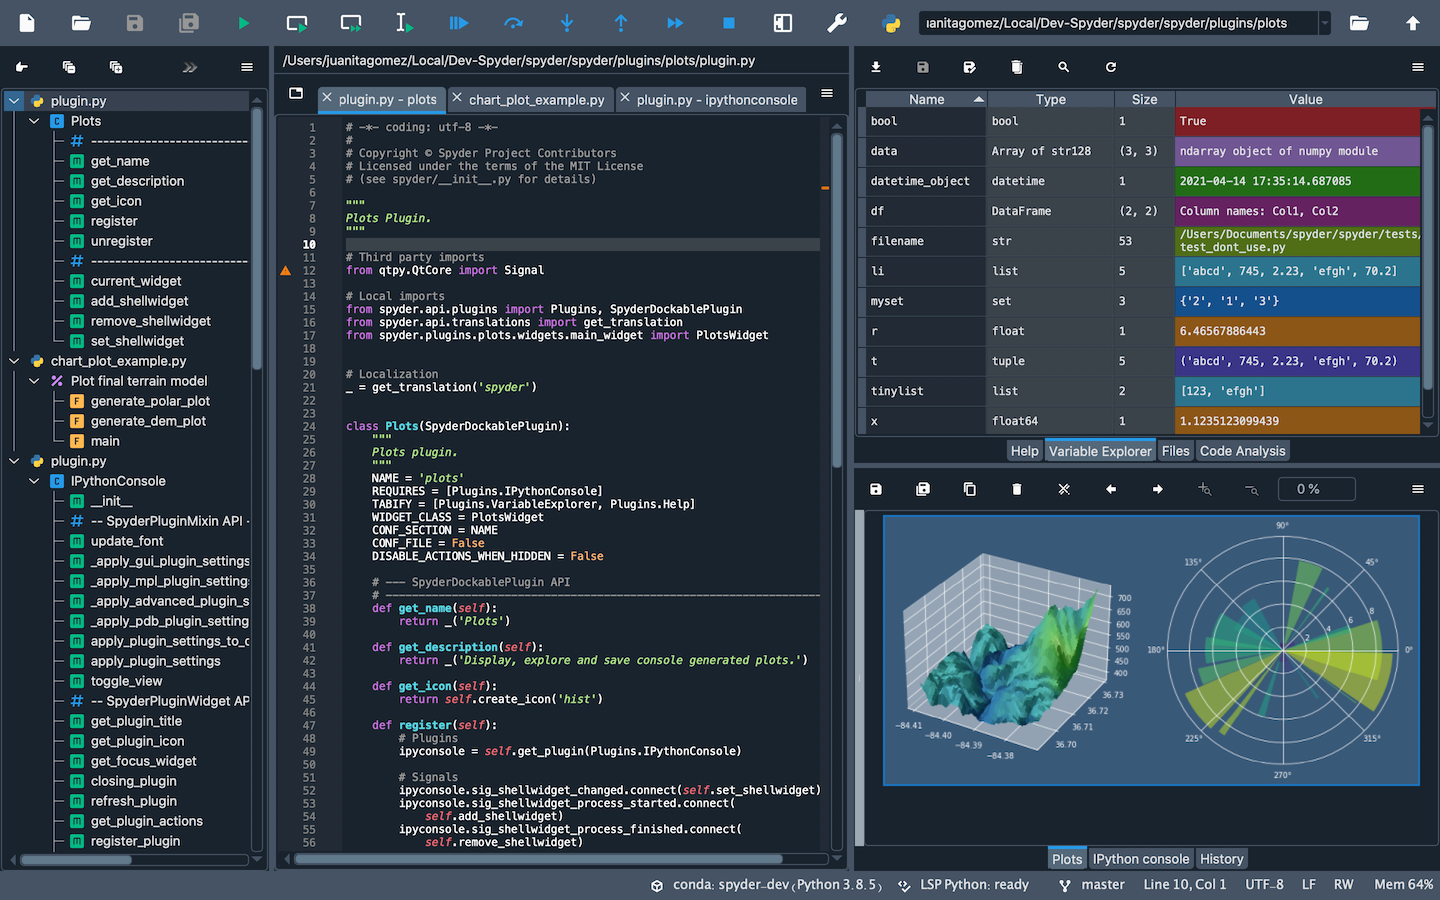
\includegraphics{figures/spyder.png}

}

\caption{\label{fig-spyder}Spyder (Source:
\href{https://docs.spyder-ide.org/current/index.html}{Spyder})}

\end{figure}%

Jupyter Notebook is a browser-based interactive tool that allows for
live code, equations, visualizations, and narrative text. JupyterLab is
the next-generation user interface that includes notebooks and offers
IDE-like features. Figure~\ref{fig-jupyter} shows the JupyterLab
interface.

\begin{figure}

\centering{

\includegraphics{figures/jupyterlab.webp}

}

\caption{\label{fig-jupyter}JupyterLab (Source:
\href{https://docs.jupyter.org/en/latest/}{Project Jupyter})}

\end{figure}%

\section{Modules}\label{modules}

Anaconda includes most of the modules needed for econometric analysis.
One of the installed modules is NumPy. To access the square root
function in NumPy, we can use one of the following ways:

\begin{Shaded}
\begin{Highlighting}[]
\CommentTok{\# First way}
\ImportTok{import}\NormalTok{ numpy}
\NormalTok{numpy.sqrt(}\DecValTok{3}\NormalTok{) }\CommentTok{\# return the squared root of 3}

\CommentTok{\# Second way}
\ImportTok{import}\NormalTok{ numpy }\ImportTok{as}\NormalTok{ np }
\NormalTok{np.sqrt(}\DecValTok{3}\NormalTok{) }\CommentTok{\# return the squared root of 3}

\CommentTok{\# Third way}
\ImportTok{from}\NormalTok{ numpy }\ImportTok{import}\OperatorTok{*} 
\NormalTok{sqrt(}\DecValTok{3}\NormalTok{) }\CommentTok{\# return the squared root of 3}

\CommentTok{\# Fourth way}
\ImportTok{from}\NormalTok{ numpy }\ImportTok{import}\NormalTok{ sqrt}
\NormalTok{sqrt(}\DecValTok{3}\NormalTok{)}
\end{Highlighting}
\end{Shaded}

In the above code chunk, the hash mark \texttt{\#} is used to add
comments to the code chunk. The text following the mark is ignored by
the Python shell. In the third way, \texttt{from\ numpy\ import*} makes
all functions in \texttt{numpy} available. In the fourth way,
\texttt{from\ numpy\ import\ sqrt} only makes the \texttt{sqrt} function
available. We recommend using the second way,
\texttt{import\ numpy\ as\ np}, and accessing the square root function
with \texttt{np.sqrt}.

In Python, \textbf{attributes} of objects are accessed using dot
notation. The term following the dot is called an attribute of the
object. An attribute can contain auxiliary information related to the
object or it can act like functions, called methods (Sheppard (2021)).
In the example \texttt{np.sqrt(3)}, \texttt{sqrt} is a method (or
function) of the \texttt{np} object.

We list some important modules that are required for econometric
analysis below:

\begin{itemize}
\item
  \texttt{numpy}: This core package for numerical computation provides
  array and matrix data types, as well as functions for linear algebra
  and random number generation. For more information, see
  \url{https://numpy.org/}.
\item
  \texttt{scipy}: SciPy includes tools for statistical functions, linear
  algebra, and optimization. For more information, see
  \url{https://www.scipy.org/}.
\item
  \texttt{matplotlib}: This library offers a versatile plotting
  environment for creating visualizations. To explore its features, see
  \url{https://matplotlib.org/}.
\item
  \texttt{seaborn}: Seaborn enhances the appearance of plots with
  improved default settings. For more information, see
  \url{https://seaborn.pydata.org}.
\item
  \texttt{pandas}: Pandas provides user-friendly data structures (series
  and dataframes) and data analysis capabilities. For more information,
  see \url{https://pandas.pydata.org}.
\item
  \texttt{statsmodels}: This module provides tools for estimating
  classical econometric models, such as linear regression models (linear
  regression, generalized linear models, robust linear models, linear
  mixed effects models, logit, probit, etc.), time series models (AR,
  ARMA, ARIMA, VAR, etc.), and nonparametric models (such as kernel
  density estimation and kernel regression). For more information, see
  \url{https://www.statsmodels.org/stable/index.html}.
\item
  \texttt{scikit-learn}: This module contains various machine learning
  methods, including classification, clustering, regression (such as
  lasso, ridge, elastic-net, support vector machines, decision trees,
  etc.), model selection, and dimensionality reduction methods. For more
  information, see \url{https://scikit-learn.org/stable}.
\end{itemize}

\section{Installing Additional
Modules}\label{installing-additional-modules}

To check all available modules in Anaconda, use the \texttt{conda\ list}
command in the Anaconda Prompt. To see if a specific module is
available, use the
\texttt{conda\ list\ \textless{}module\_name\textgreater{}} command. If
the module is not included in Anaconda, it must be installed manually.
For example, to install the \texttt{wooldridge} module, which is used
for econometric analysis, we can type \texttt{pip\ install\ wooldridge}
in the Anaconda Prompt or in the Python shell. The \texttt{pip} command
is a package manager for Python that allows you to install and manage
additional modules not included in the Anaconda distribution.

\section{Variable Assignment}\label{variable-assignment}

In Python, the assignment operator is the equality symbol \texttt{=}.
Consider the following examples:

\begin{Shaded}
\begin{Highlighting}[]
\CommentTok{\# Assigning a value to a variable}
\NormalTok{x }\OperatorTok{=} \DecValTok{3}
\NormalTok{x}
\end{Highlighting}
\end{Shaded}

\begin{verbatim}
3
\end{verbatim}

\begin{Shaded}
\begin{Highlighting}[]
\CommentTok{\# Assigning strings to a variable}
\NormalTok{y }\OperatorTok{=} \StringTok{"abc"}
\NormalTok{y}
\end{Highlighting}
\end{Shaded}

\begin{verbatim}
'abc'
\end{verbatim}

\begin{Shaded}
\begin{Highlighting}[]
\CommentTok{\# Multiple assignments}
\NormalTok{x, y, z }\OperatorTok{=} \DecValTok{1}\NormalTok{, }\FloatTok{3.1415}\NormalTok{, }\StringTok{"abcd"}
\NormalTok{x, y, z}
\end{Highlighting}
\end{Shaded}

\begin{verbatim}
(1, 3.1415, 'abcd')
\end{verbatim}

The \texttt{dir} command or the magic command \texttt{\%whos} in IPython
can be used to list all variables defined in the current session. This
is useful for checking the variables you have created during your
session.

\begin{Shaded}
\begin{Highlighting}[]
\CommentTok{\# List all variables in the Python shell}
\BuiltInTok{print}\NormalTok{(}\BuiltInTok{dir}\NormalTok{())}
\end{Highlighting}
\end{Shaded}

\begin{verbatim}
['In', 'InteractiveShell', 'Out', '_', '_2', '_3', '_4', '__', '___', '__builtin__', '__builtins__', '__name__', '_dh', '_i', '_i1', '_i2', '_i3', '_i4', '_i5', '_ih', '_ii', '_iii', '_oh', 'exit', 'get_ipython', 'ojs_define', 'open', 'quit', 'x', 'y', 'z']
\end{verbatim}

\section{Built-in Data Types}\label{built-in-data-types}

Some useful built-in data types and structures are

\begin{itemize}
\tightlist
\item
  numeric types,
\item
  booleans,
\item
  strings,
\item
  lists,
\item
  tuples,
\item
  dictionary,
\item
  sets, and
\item
  range.
\end{itemize}

\subsection{Numeric types}\label{numeric-types}

In Python, simple numbers can be either integers, floats, or complex
numbers. We can use the \texttt{type} function to get the type of the
object. Consider the following examples:

\begin{Shaded}
\begin{Highlighting}[]
\CommentTok{\# Integer}
\NormalTok{x }\OperatorTok{=} \DecValTok{3}
\BuiltInTok{type}\NormalTok{(x)}
\end{Highlighting}
\end{Shaded}

\begin{verbatim}
int
\end{verbatim}

\begin{Shaded}
\begin{Highlighting}[]
\CommentTok{\# Float}
\NormalTok{x }\OperatorTok{=} \FloatTok{3.2}
\BuiltInTok{type}\NormalTok{(x)}
\end{Highlighting}
\end{Shaded}

\begin{verbatim}
float
\end{verbatim}

\begin{Shaded}
\begin{Highlighting}[]
\CommentTok{\# Complex}
\NormalTok{x }\OperatorTok{=} \DecValTok{2} \OperatorTok{+} \OtherTok{3j}
\BuiltInTok{type}\NormalTok{(x)}
\end{Highlighting}
\end{Shaded}

\begin{verbatim}
complex
\end{verbatim}

Some built-in binary operators are listed below:

\begin{itemize}
\tightlist
\item
  addition: \texttt{x+y}
\item
  subtraction: \texttt{x-y}
\item
  multiplication: \texttt{x*y}
\item
  division: \texttt{x/y}
\item
  integer division: \texttt{x//y}=\(\lfloor\frac{x}{y}\rfloor\)
\item
  exponentiation: \texttt{x**y}=\(x^y\)
\end{itemize}

Consider the following examples:

\begin{Shaded}
\begin{Highlighting}[]
\NormalTok{x, y }\OperatorTok{=} \DecValTok{3}\NormalTok{, }\DecValTok{2}
\NormalTok{x }\OperatorTok{+}\NormalTok{ y  }\CommentTok{\# returns 5}
\end{Highlighting}
\end{Shaded}

\begin{verbatim}
5
\end{verbatim}

\begin{Shaded}
\begin{Highlighting}[]
\NormalTok{x }\OperatorTok{*}\NormalTok{ y  }\CommentTok{\# returns 6}
\end{Highlighting}
\end{Shaded}

\begin{verbatim}
6
\end{verbatim}

\begin{Shaded}
\begin{Highlighting}[]
\NormalTok{x }\OperatorTok{//}\NormalTok{ y }\CommentTok{\# returns 1}
\end{Highlighting}
\end{Shaded}

\begin{verbatim}
1
\end{verbatim}

\begin{Shaded}
\begin{Highlighting}[]
\NormalTok{x}\OperatorTok{**}\NormalTok{y  }\CommentTok{\# returns 9}
\end{Highlighting}
\end{Shaded}

\begin{verbatim}
9
\end{verbatim}

\subsection{Boolean}\label{boolean}

In Python, the Boolean data type is used to represent truth values, with
\texttt{True} and \texttt{False} as the reserved keywords.

\begin{Shaded}
\begin{Highlighting}[]
\NormalTok{x }\OperatorTok{=} \VariableTok{True}
\BuiltInTok{type}\NormalTok{(x)}
\end{Highlighting}
\end{Shaded}

\begin{verbatim}
bool
\end{verbatim}

\begin{Shaded}
\begin{Highlighting}[]
\BuiltInTok{bool}\NormalTok{(}\DecValTok{1}\NormalTok{)}
\end{Highlighting}
\end{Shaded}

\begin{verbatim}
True
\end{verbatim}

\begin{Shaded}
\begin{Highlighting}[]
\BuiltInTok{bool}\NormalTok{(}\DecValTok{0}\NormalTok{)}
\end{Highlighting}
\end{Shaded}

\begin{verbatim}
False
\end{verbatim}

Note that non-zero and non-empty values generally evaluate to
\texttt{True} when passed to \texttt{bool()}. Conversely, zero or empty
values, such as \texttt{bool(0)}, \texttt{bool(0.0)},
\texttt{bool(0.0j)}, \texttt{bool(None)}, and \texttt{bool({[}{]})}, all
evaluate to \texttt{False}.

Some built-in binary operators returning \texttt{True} and
\texttt{False} are listed below:

\begin{itemize}
\tightlist
\item
  \texttt{a\ \&\ b}: True if both \texttt{a} and \texttt{b} are True
\item
  \texttt{a\ \textbar{}\ b}: True if either \texttt{a} or \texttt{b} is
  True
\item
  \texttt{a\ ==\ b}: True if \texttt{a} equals \texttt{b}
\item
  \texttt{a\ !=\ b}: True if \texttt{a} is not equal to \texttt{b}
\item
  \texttt{a\ \textless{}\ b}, \texttt{a\ \textless{}=\ b}: True if
  \texttt{a} is less than (less than or equal to) \texttt{b}
\item
  \texttt{a\ \textgreater{}\ b}, \texttt{a\ \textgreater{}=\ b}: True if
  \texttt{a} is greater than (greater than or equal to) \texttt{b}
\end{itemize}

Some illustrative examples are given below.

\begin{Shaded}
\begin{Highlighting}[]
\NormalTok{a }\OperatorTok{=} \VariableTok{True}
\NormalTok{b }\OperatorTok{=} \VariableTok{True}
\NormalTok{a }\OperatorTok{\&}\NormalTok{ b  }\CommentTok{\# returns True}
\end{Highlighting}
\end{Shaded}

\begin{verbatim}
True
\end{verbatim}

\begin{Shaded}
\begin{Highlighting}[]
\NormalTok{a }\OperatorTok{==}\NormalTok{ b  }\CommentTok{\# returns True}
\end{Highlighting}
\end{Shaded}

\begin{verbatim}
True
\end{verbatim}

\begin{Shaded}
\begin{Highlighting}[]
\NormalTok{a, b }\OperatorTok{=} \DecValTok{18}\NormalTok{, }\DecValTok{4}
\NormalTok{a }\OperatorTok{\textless{}=}\NormalTok{ b  }\CommentTok{\# returns False}
\end{Highlighting}
\end{Shaded}

\begin{verbatim}
False
\end{verbatim}

\subsection{Strings}\label{strings}

In Python, strings can be enclosed in either single quotes
\texttt{\textquotesingle{}string\textquotesingle{}} or double quotes
\texttt{"string"}.

\begin{Shaded}
\begin{Highlighting}[]
\CommentTok{\# Assigning a string to a variable}
\NormalTok{x }\OperatorTok{=} \StringTok{"This is a string"}
\BuiltInTok{type}\NormalTok{(x)}
\NormalTok{x}
\end{Highlighting}
\end{Shaded}

\begin{verbatim}
str
\end{verbatim}

\begin{verbatim}
'This is a string'
\end{verbatim}

In Python, slicing employs \texttt{{[}\ {]}} to specify the indices of
the characters in a string. Python uses \textbf{0-based indexing}.
Suppose that \texttt{s} has n characters. Then,

\begin{itemize}
\tightlist
\item
  \texttt{s{[}:{]}}: returns entire string,
\item
  \texttt{s{[}i{]}}: returns character at index \(i\),
\item
  \texttt{s{[}i:{]}}: returns characters with indices \(i,\dots,n-1\),
\item
  \texttt{s{[}:i{]}}: returns characters with indices \(0,\dots,i-1\),
\item
  \texttt{s{[}i:j{]}}: returns characters with indices \(i,\dots,j-1\),
\item
  \texttt{s{[}i:j:m{]}}: returns characters with indices
  \(i,i+m,i+2m,\dots,i+m\lfloor\frac{j-i-1}{m}\rfloor\),
\item
  \texttt{s{[}-i{]}}: returns characters at index \(n-i\).
\end{itemize}

The following examples illustrate string slicing.

\begin{Shaded}
\begin{Highlighting}[]
\NormalTok{s }\OperatorTok{=} \StringTok{"Python strings are sliceable."}
\BuiltInTok{len}\NormalTok{(s)  }\CommentTok{\# returns the length of the string}
\end{Highlighting}
\end{Shaded}

\begin{verbatim}
29
\end{verbatim}

\begin{Shaded}
\begin{Highlighting}[]
\NormalTok{s[}\DecValTok{0}\NormalTok{] }\CommentTok{\# returns the first character}
\end{Highlighting}
\end{Shaded}

\begin{verbatim}
'P'
\end{verbatim}

\begin{Shaded}
\begin{Highlighting}[]
\NormalTok{L }\OperatorTok{=} \BuiltInTok{len}\NormalTok{(s)}
\NormalTok{s[L }\OperatorTok{{-}} \DecValTok{1}\NormalTok{]  }\CommentTok{\# returns the last character}
\end{Highlighting}
\end{Shaded}

\begin{verbatim}
'.'
\end{verbatim}

\begin{Shaded}
\begin{Highlighting}[]
\NormalTok{s[:}\DecValTok{10}\NormalTok{] }\CommentTok{\# returns the first 9 characters (including space)}
\end{Highlighting}
\end{Shaded}

\begin{verbatim}
'Python str'
\end{verbatim}

\begin{Shaded}
\begin{Highlighting}[]
\NormalTok{s[}\DecValTok{10}\NormalTok{:] }\CommentTok{\# returns the characters from index 10 to the end}
\end{Highlighting}
\end{Shaded}

\begin{verbatim}
'ings are sliceable.'
\end{verbatim}

\subsection{Lists}\label{lists}

A list is a collection of objects constructed using square brackets
\texttt{{[}\ {]}}, with values separated by commas. Some illustrative
examples are given in the following.

\begin{Shaded}
\begin{Highlighting}[]
\NormalTok{x }\OperatorTok{=}\NormalTok{ [}\DecValTok{1}\NormalTok{, }\DecValTok{2}\NormalTok{, }\DecValTok{3}\NormalTok{, }\DecValTok{4}\NormalTok{]}
\BuiltInTok{type}\NormalTok{(x)}
\NormalTok{x}
\end{Highlighting}
\end{Shaded}

\begin{verbatim}
list
\end{verbatim}

\begin{verbatim}
[1, 2, 3, 4]
\end{verbatim}

\begin{Shaded}
\begin{Highlighting}[]
\CommentTok{\# A list of lists}
\NormalTok{y }\OperatorTok{=}\NormalTok{ [[}\DecValTok{1}\NormalTok{, }\DecValTok{2}\NormalTok{, }\DecValTok{3}\NormalTok{, }\DecValTok{4}\NormalTok{], [}\DecValTok{5}\NormalTok{, }\DecValTok{6}\NormalTok{, }\DecValTok{7}\NormalTok{]]}
\NormalTok{y}
\end{Highlighting}
\end{Shaded}

\begin{verbatim}
[[1, 2, 3, 4], [5, 6, 7]]
\end{verbatim}

\begin{Shaded}
\begin{Highlighting}[]
\CommentTok{\# A list can contain different data types}
\NormalTok{z }\OperatorTok{=}\NormalTok{ [}\DecValTok{1}\NormalTok{, }\FloatTok{1.0}\NormalTok{, }\DecValTok{1} \OperatorTok{+} \OtherTok{0j}\NormalTok{, }\StringTok{"one"}\NormalTok{, }\VariableTok{None}\NormalTok{, }\VariableTok{True}\NormalTok{, }\VariableTok{False}\NormalTok{, }\StringTok{"abc"}\NormalTok{]}
\NormalTok{z}
\end{Highlighting}
\end{Shaded}

\begin{verbatim}
[1, 1.0, (1+0j), 'one', None, True, False, 'abc']
\end{verbatim}

List slicing is similar to string slicing. Let \(x\) be a list with
\(n\) elements denoted by \(x_0,x_1,\dots,x_{n-1}\).

\begin{itemize}
\tightlist
\item
  \texttt{x{[}:{]}}: returns \(x\)
\item
  \texttt{x{[}i{]}}: returns \(x_i\)
\item
  \texttt{x{[}i:{]}}: returns \(x_i,\dots,x_{n-1}\)
\item
  \texttt{x{[}:i{]}}: returns \(x_0,\dots,x_{i-1}\)
\item
  \texttt{x{[}i:j{]}}: returns \(x_i,\dots,x_{j-1}\)
\item
  \texttt{x{[}i:j:m{]}}: returns
  \(x_i,x_{i+m},x_{i+2m},\dots,x_{i+m\lfloor\frac{j-i-1}{m}\rfloor}\)
\item
  \texttt{x{[}-i{]}}: return \(x_{n-i}\)
\end{itemize}

Consider the following examples:

\begin{Shaded}
\begin{Highlighting}[]
\NormalTok{x }\OperatorTok{=}\NormalTok{ [[}\DecValTok{1}\NormalTok{, }\DecValTok{2}\NormalTok{, }\DecValTok{3}\NormalTok{, }\DecValTok{4}\NormalTok{], [}\DecValTok{5}\NormalTok{, }\DecValTok{6}\NormalTok{, }\DecValTok{7}\NormalTok{, }\DecValTok{8}\NormalTok{]]}
\NormalTok{x[}\DecValTok{0}\NormalTok{]  }\CommentTok{\# the first element of the list x}
\end{Highlighting}
\end{Shaded}

\begin{verbatim}
[1, 2, 3, 4]
\end{verbatim}

\begin{Shaded}
\begin{Highlighting}[]
\CommentTok{\# the first element of the first element of the list x}
\NormalTok{x[}\DecValTok{0}\NormalTok{][}\DecValTok{0}\NormalTok{]}
\end{Highlighting}
\end{Shaded}

\begin{verbatim}
1
\end{verbatim}

\begin{Shaded}
\begin{Highlighting}[]
\CommentTok{\# the second, third, and fourth elements of the first element of the list}
\NormalTok{x[}\DecValTok{0}\NormalTok{][}\DecValTok{1}\NormalTok{:}\DecValTok{4}\NormalTok{] }
\NormalTok{x}
\end{Highlighting}
\end{Shaded}

\begin{verbatim}
[2, 3, 4]
\end{verbatim}

\begin{verbatim}
[[1, 2, 3, 4], [5, 6, 7, 8]]
\end{verbatim}

In Table~\ref{tbl-t1.1}, we provide some useful functions that can be
used to manipulate lists.

\begin{figure}

\begin{minipage}{\linewidth}

\begin{longtable}[]{@{}
  >{\raggedright\arraybackslash}p{(\columnwidth - 4\tabcolsep) * \real{0.3056}}
  >{\raggedright\arraybackslash}p{(\columnwidth - 4\tabcolsep) * \real{0.2500}}
  >{\raggedright\arraybackslash}p{(\columnwidth - 4\tabcolsep) * \real{0.4444}}@{}}
\caption{Some useful list functions and
methods}\label{tbl-t1.1}\tabularnewline
\toprule\noalign{}
\begin{minipage}[b]{\linewidth}\raggedright
Function
\end{minipage} & \begin{minipage}[b]{\linewidth}\raggedright
Method
\end{minipage} & \begin{minipage}[b]{\linewidth}\raggedright
Description
\end{minipage} \\
\midrule\noalign{}
\endfirsthead
\toprule\noalign{}
\begin{minipage}[b]{\linewidth}\raggedright
Function
\end{minipage} & \begin{minipage}[b]{\linewidth}\raggedright
Method
\end{minipage} & \begin{minipage}[b]{\linewidth}\raggedright
Description
\end{minipage} \\
\midrule\noalign{}
\endhead
\bottomrule\noalign{}
\endlastfoot
\texttt{list.append(x,value)} & \texttt{x.append(value)} & Appends value
to the end of the list. \\
\texttt{len(x)} & - & Returns the number of elements in the list. \\
\texttt{list.extend(x,list)} & \texttt{x.extend(list)} & Appends the
values in list to the existing list. \\
\texttt{list.pop(x,index)} & \texttt{x.pop(index)} & Removes the value
in position index and returns the value. \\
\texttt{list.remove(x,value)} & \texttt{x.remove(value)} & Removes the
first occurrence of value from the list. \\
\texttt{list.count(x,value)} & \texttt{x.count(value)} & Counts the
number of occurrences of value in the list. \\
\texttt{del\ x{[}slice{]}} & - & Deletes the elements in slice. \\
\end{longtable}

\end{minipage}%

\end{figure}%

Some illustrative examples are provided below.

\begin{Shaded}
\begin{Highlighting}[]
\CommentTok{\# Appending a value to the end of the list}
\NormalTok{x }\OperatorTok{=}\NormalTok{ [}\DecValTok{0}\NormalTok{, }\DecValTok{1}\NormalTok{, }\DecValTok{2}\NormalTok{, }\DecValTok{3}\NormalTok{, }\DecValTok{4}\NormalTok{, }\DecValTok{5}\NormalTok{, }\DecValTok{6}\NormalTok{, }\DecValTok{7}\NormalTok{, }\DecValTok{8}\NormalTok{, }\DecValTok{9}\NormalTok{]}
\NormalTok{x.append(}\DecValTok{0}\NormalTok{)}
\NormalTok{x}
\end{Highlighting}
\end{Shaded}

\begin{verbatim}
[0, 1, 2, 3, 4, 5, 6, 7, 8, 9, 0]
\end{verbatim}

\begin{Shaded}
\begin{Highlighting}[]
\CommentTok{\# Appending a list to the end of the list}
\NormalTok{x.extend([}\DecValTok{11}\NormalTok{, }\DecValTok{12}\NormalTok{, }\DecValTok{13}\NormalTok{, }\DecValTok{0}\NormalTok{])}
\NormalTok{x}
\end{Highlighting}
\end{Shaded}

\begin{verbatim}
[0, 1, 2, 3, 4, 5, 6, 7, 8, 9, 0, 11, 12, 13, 0]
\end{verbatim}

\begin{Shaded}
\begin{Highlighting}[]
\CommentTok{\# Remove the element at index 1 and return it}
\NormalTok{x.pop(}\DecValTok{1}\NormalTok{)}
\NormalTok{x}
\end{Highlighting}
\end{Shaded}

\begin{verbatim}
1
\end{verbatim}

\begin{verbatim}
[0, 2, 3, 4, 5, 6, 7, 8, 9, 0, 11, 12, 13, 0]
\end{verbatim}

\begin{Shaded}
\begin{Highlighting}[]
\CommentTok{\# Remove the first occurrence of 0 from the list}
\NormalTok{x.remove(}\DecValTok{0}\NormalTok{)}
\NormalTok{x}
\end{Highlighting}
\end{Shaded}

\begin{verbatim}
[2, 3, 4, 5, 6, 7, 8, 9, 0, 11, 12, 13, 0]
\end{verbatim}

\subsection{Tuples}\label{tuples}

A tuple is similar to a list with one important difference: tuples are
immutable. Immutability means that once a tuple is created, it cannot be
modified. Tuples are created using \texttt{()} with elements separated
by commas. Some illustrative examples are provided below.

\begin{Shaded}
\begin{Highlighting}[]
\NormalTok{x }\OperatorTok{=}\NormalTok{ (}\DecValTok{1}\NormalTok{, }\DecValTok{2}\NormalTok{, }\DecValTok{3}\NormalTok{, }\DecValTok{4}\NormalTok{, }\DecValTok{5}\NormalTok{, }\DecValTok{6}\NormalTok{, }\DecValTok{7}\NormalTok{, }\StringTok{"a"}\NormalTok{, }\StringTok{"abc"}\NormalTok{, }\StringTok{"ABC"}\NormalTok{)}
\BuiltInTok{type}\NormalTok{(x)}
\end{Highlighting}
\end{Shaded}

\begin{verbatim}
tuple
\end{verbatim}

\begin{Shaded}
\begin{Highlighting}[]
\CommentTok{\# The first element of the tuple}
\NormalTok{x[}\DecValTok{0}\NormalTok{]}
\end{Highlighting}
\end{Shaded}

\begin{verbatim}
1
\end{verbatim}

\begin{Shaded}
\begin{Highlighting}[]
\CommentTok{\# Elements at indices 5 to 9}
\NormalTok{x[}\DecValTok{5}\NormalTok{:}\DecValTok{10}\NormalTok{]}
\end{Highlighting}
\end{Shaded}

\begin{verbatim}
(6, 7, 'a', 'abc', 'ABC')
\end{verbatim}

\begin{Shaded}
\begin{Highlighting}[]
\CommentTok{\# Converting a tuple to a list}
\NormalTok{x }\OperatorTok{=} \BuiltInTok{list}\NormalTok{(x) }
\BuiltInTok{type}\NormalTok{(x)}
\end{Highlighting}
\end{Shaded}

\begin{verbatim}
list
\end{verbatim}

\begin{Shaded}
\begin{Highlighting}[]
\CommentTok{\# Converting a list back to a tuple}
\NormalTok{x }\OperatorTok{=} \BuiltInTok{tuple}\NormalTok{(x) }
\BuiltInTok{type}\NormalTok{(x)}
\end{Highlighting}
\end{Shaded}

\begin{verbatim}
tuple
\end{verbatim}

\begin{Shaded}
\begin{Highlighting}[]
\CommentTok{\# A tuple of lists}
\NormalTok{x }\OperatorTok{=}\NormalTok{ ([}\DecValTok{1}\NormalTok{, }\DecValTok{2}\NormalTok{], [}\DecValTok{3}\NormalTok{, }\DecValTok{4}\NormalTok{])}
\BuiltInTok{type}\NormalTok{(x)}
\end{Highlighting}
\end{Shaded}

\begin{verbatim}
tuple
\end{verbatim}

\begin{Shaded}
\begin{Highlighting}[]
\CommentTok{\# The second element of the tuple}
\NormalTok{x[}\DecValTok{1}\NormalTok{] }
\end{Highlighting}
\end{Shaded}

\begin{verbatim}
[3, 4]
\end{verbatim}

\subsection{Dictionary (dict)}\label{dictionary-dict}

In Python, dictionaries are data structures that store pairs of keys
(words) and values (definitions). Dictionaries are created using the
following syntax:
\texttt{\{\textquotesingle{}key\textquotesingle{}:value\}}. You can
access a value using its corresponding key. Some illustrative examples
are given below.

\begin{Shaded}
\begin{Highlighting}[]
\CommentTok{\# Creating a dictionary with three key{-}value pairs}
\NormalTok{data }\OperatorTok{=}\NormalTok{ \{}\StringTok{"age"}\NormalTok{: }\DecValTok{34}\NormalTok{, }\StringTok{"children"}\NormalTok{: [}\DecValTok{1}\NormalTok{, }\DecValTok{2}\NormalTok{], }\DecValTok{1}\NormalTok{: }\StringTok{"apple"}\NormalTok{\}}
\BuiltInTok{type}\NormalTok{(data)}
\end{Highlighting}
\end{Shaded}

\begin{verbatim}
dict
\end{verbatim}

\begin{Shaded}
\begin{Highlighting}[]
\CommentTok{\# Accessing the value associated with the key \textquotesingle{}children\textquotesingle{}}
\NormalTok{data[}\StringTok{\textquotesingle{}children\textquotesingle{}}\NormalTok{]}
\end{Highlighting}
\end{Shaded}

\begin{verbatim}
[1, 2]
\end{verbatim}

\begin{Shaded}
\begin{Highlighting}[]
\CommentTok{\# Changing the value associated with the key \textquotesingle{}age\textquotesingle{}}
\NormalTok{data[}\StringTok{"age"}\NormalTok{] }\OperatorTok{=} \StringTok{"40"}
\NormalTok{data}
\end{Highlighting}
\end{Shaded}

\begin{verbatim}
{'age': '40', 'children': [1, 2], 1: 'apple'}
\end{verbatim}

\begin{Shaded}
\begin{Highlighting}[]
\CommentTok{\# Adding a new key{-}value pair}
\NormalTok{data[}\StringTok{"name"}\NormalTok{] }\OperatorTok{=} \StringTok{"Joe"}
\NormalTok{data}
\end{Highlighting}
\end{Shaded}

\begin{verbatim}
{'age': '40', 'children': [1, 2], 1: 'apple', 'name': 'Joe'}
\end{verbatim}

\begin{Shaded}
\begin{Highlighting}[]
\CommentTok{\# Deleting a key{-}value pair}
\KeywordTok{del}\NormalTok{ data[}\StringTok{"age"}\NormalTok{]}
\NormalTok{data}
\end{Highlighting}
\end{Shaded}

\begin{verbatim}
{'children': [1, 2], 1: 'apple', 'name': 'Joe'}
\end{verbatim}

\subsection{Sets}\label{sets}

Sets are collections of unique objects. In Python, you can create a set
using the \texttt{set()} function. Some illustrative examples are shown
below.

\begin{Shaded}
\begin{Highlighting}[]
\CommentTok{\# Creating a set with some fruits}
\NormalTok{x }\OperatorTok{=} \BuiltInTok{set}\NormalTok{([}\StringTok{"Apple"}\NormalTok{, }\StringTok{"Orange"}\NormalTok{, }\StringTok{"Banana"}\NormalTok{, }\StringTok{"Fig"}\NormalTok{, }\StringTok{"Apricot"}\NormalTok{])}
\BuiltInTok{type}\NormalTok{(x)}
\NormalTok{x}
\end{Highlighting}
\end{Shaded}

\begin{verbatim}
set
\end{verbatim}

\begin{verbatim}
{'Apple', 'Apricot', 'Banana', 'Fig', 'Orange'}
\end{verbatim}

\begin{Shaded}
\begin{Highlighting}[]
\CommentTok{\# Adding a new element to the set}
\NormalTok{x.add(}\StringTok{"Cherry"}\NormalTok{)}
\NormalTok{x}
\end{Highlighting}
\end{Shaded}

\begin{verbatim}
{'Apple', 'Apricot', 'Banana', 'Cherry', 'Fig', 'Orange'}
\end{verbatim}

\begin{Shaded}
\begin{Highlighting}[]
\CommentTok{\# Intersection of two sets}
\NormalTok{y }\OperatorTok{=} \BuiltInTok{set}\NormalTok{([}\StringTok{"Coconut"}\NormalTok{, }\StringTok{"Fig"}\NormalTok{, }\StringTok{"Apricot"}\NormalTok{])}
\NormalTok{x.intersection(y)}
\end{Highlighting}
\end{Shaded}

\begin{verbatim}
{'Apricot', 'Fig'}
\end{verbatim}

\begin{Shaded}
\begin{Highlighting}[]
\CommentTok{\# Union of two sets}
\NormalTok{x }\OperatorTok{=}\NormalTok{ x.union(y)}
\NormalTok{x}
\end{Highlighting}
\end{Shaded}

\begin{verbatim}
{'Apple', 'Apricot', 'Banana', 'Cherry', 'Coconut', 'Fig', 'Orange'}
\end{verbatim}

\begin{Shaded}
\begin{Highlighting}[]
\CommentTok{\# Removing an element from the set}
\NormalTok{x.remove(}\StringTok{"Fig"}\NormalTok{)}
\NormalTok{x}
\end{Highlighting}
\end{Shaded}

\begin{verbatim}
{'Apple', 'Apricot', 'Banana', 'Cherry', 'Coconut', 'Orange'}
\end{verbatim}

\subsection{Range}\label{range}

The function \texttt{range(a,\ b,\ i)} generates a sequence of numbers
starting from \texttt{a} (inclusive) up to, but not including,
\texttt{b}, with an increment of \texttt{i}. Some illustrative examples
are given below.

\begin{Shaded}
\begin{Highlighting}[]
\CommentTok{\# Creating a range object from 0 to 9}
\NormalTok{x }\OperatorTok{=} \BuiltInTok{range}\NormalTok{(}\DecValTok{10}\NormalTok{)}
\BuiltInTok{type}\NormalTok{(x)}
\end{Highlighting}
\end{Shaded}

\begin{verbatim}
range
\end{verbatim}

\begin{Shaded}
\begin{Highlighting}[]
\CommentTok{\# Checking if x is a range object}
\BuiltInTok{isinstance}\NormalTok{(x, }\BuiltInTok{range}\NormalTok{)}
\end{Highlighting}
\end{Shaded}

\begin{verbatim}
True
\end{verbatim}

\begin{Shaded}
\begin{Highlighting}[]
\CommentTok{\# Printing the range object}
\BuiltInTok{print}\NormalTok{(x)}
\end{Highlighting}
\end{Shaded}

\begin{verbatim}
range(0, 10)
\end{verbatim}

\begin{Shaded}
\begin{Highlighting}[]
\CommentTok{\# Listing the elements of the range object}
\BuiltInTok{list}\NormalTok{(x) }
\end{Highlighting}
\end{Shaded}

\begin{verbatim}
[0, 1, 2, 3, 4, 5, 6, 7, 8, 9]
\end{verbatim}

\begin{Shaded}
\begin{Highlighting}[]
\CommentTok{\# Converting the range object to a list}
\NormalTok{x }\OperatorTok{=} \BuiltInTok{range}\NormalTok{(}\DecValTok{3}\NormalTok{, }\DecValTok{10}\NormalTok{, }\DecValTok{3}\NormalTok{)}
\BuiltInTok{list}\NormalTok{(x)}
\end{Highlighting}
\end{Shaded}

\begin{verbatim}
[3, 6, 9]
\end{verbatim}

\chapter{Introduction to NumPy}\label{sec-chapter2}

\section{Introduction}\label{introduction-1}

\href{https://numpy.org/}{NumPy} provides (i) array objects for storing
homogeneous data, (ii) mathematical functions for arrays, (iii) linear
algebra functions, and (iv) statistical functions for generating random
numbers. We constrain our treatment of NumPy to features that are useful
for econometric analysis. The NumPy module is usually imported under the
alias \texttt{np}, as shown in the following chunk.

\begin{Shaded}
\begin{Highlighting}[]
\ImportTok{import}\NormalTok{ numpy }\ImportTok{as}\NormalTok{ np}
\end{Highlighting}
\end{Shaded}

\[
\DeclareMathOperator{\cov}{cov}
\DeclareMathOperator{\corr}{corr} 
\DeclareMathOperator{\var}{var} 
\DeclareMathOperator{\SE}{SE} 
\DeclareMathOperator{\E}{E}
\DeclareMathOperator{\A}{\boldsymbol{A}}
\DeclareMathOperator{\x}{\boldsymbol{x}}
\DeclareMathOperator{\sgn}{sgn}  
\DeclareMathOperator{\argmin}{argmin} 
\newcommand{\tr}{\text{tr}}
\newcommand{\bs}{\boldsymbol}
\newcommand{\mb}{\mathbb}
\]

\section{Arrays}\label{arrays}

An array can be considered as a container for data of the same type.
Arrays can be initialized from lists (or tuples) using the
\texttt{np.array} function.

\begin{Shaded}
\begin{Highlighting}[]
\CommentTok{\# Initialize an array from a list}
\NormalTok{x }\OperatorTok{=}\NormalTok{ [}\FloatTok{0.0}\NormalTok{, }\DecValTok{1}\NormalTok{, }\DecValTok{2}\NormalTok{, }\DecValTok{3}\NormalTok{, }\DecValTok{4}\NormalTok{]}
\NormalTok{y }\OperatorTok{=}\NormalTok{ np.array(x)}
\BuiltInTok{type}\NormalTok{(y)}
\end{Highlighting}
\end{Shaded}

\begin{verbatim}
numpy.ndarray
\end{verbatim}

\begin{Shaded}
\begin{Highlighting}[]
\NormalTok{y}
\end{Highlighting}
\end{Shaded}

\begin{verbatim}
array([0., 1., 2., 3., 4.])
\end{verbatim}

Attributes of an array includes \texttt{ndim} (the number of dimension),
\texttt{shape} (the size of each dimension), \texttt{size} (the total
number of elements), and \texttt{dtype} (the data type). Consider the
following examples:

\begin{Shaded}
\begin{Highlighting}[]
\NormalTok{y }\OperatorTok{=}\NormalTok{ np.array([}\FloatTok{0.0}\NormalTok{, }\DecValTok{1}\NormalTok{, }\DecValTok{2}\NormalTok{, }\DecValTok{3}\NormalTok{, }\DecValTok{4}\NormalTok{, }\DecValTok{5}\NormalTok{, }\DecValTok{6}\NormalTok{, }\DecValTok{7}\NormalTok{, }\DecValTok{8}\NormalTok{, }\DecValTok{9}\NormalTok{])}
\NormalTok{y}
\NormalTok{y.shape }\CommentTok{\# The size of each dimension}
\NormalTok{y.ndim  }\CommentTok{\# The number of dimensions}
\NormalTok{y.size  }\CommentTok{\# The total number of elements}
\NormalTok{y.dtype }\CommentTok{\# The data type of the elements}
\end{Highlighting}
\end{Shaded}

\begin{verbatim}
array([0., 1., 2., 3., 4., 5., 6., 7., 8., 9.])
\end{verbatim}

\begin{verbatim}
(10,)
\end{verbatim}

\begin{verbatim}
1
\end{verbatim}

\begin{verbatim}
10
\end{verbatim}

\begin{verbatim}
dtype('float64')
\end{verbatim}

We can create row vectors from 1-dimensional arrays. For example,
\(x = [1,2,3]\) can be entered as

\begin{Shaded}
\begin{Highlighting}[]
\NormalTok{x }\OperatorTok{=}\NormalTok{ np.array([}\DecValTok{1}\NormalTok{, }\DecValTok{2}\NormalTok{, }\DecValTok{3}\NormalTok{])}
\NormalTok{x}
\NormalTok{x.shape}
\NormalTok{x.ndim}
\end{Highlighting}
\end{Shaded}

\begin{verbatim}
array([1, 2, 3])
\end{verbatim}

\begin{verbatim}
(3,)
\end{verbatim}

\begin{verbatim}
1
\end{verbatim}

Nested lists can be used to create higher-dimensional arrays. The number
of dimensions is determined by the level of nesting. A simple list
creates a one-dimensional array. A two-dimensional array requires a
nested list with one level of nesting. Higher-dimensional arrays require
additional levels of nesting. Some examples are provided below.

\begin{Shaded}
\begin{Highlighting}[]
\CommentTok{\# A 2{-}dimensional array}
\NormalTok{x }\OperatorTok{=}\NormalTok{ np.array([[}\DecValTok{1}\NormalTok{, }\DecValTok{2}\NormalTok{, }\DecValTok{3}\NormalTok{], [}\DecValTok{2}\NormalTok{, }\DecValTok{3}\NormalTok{, }\DecValTok{10}\NormalTok{]])}
\NormalTok{x}
\NormalTok{x.shape}
\NormalTok{x.ndim}
\NormalTok{x.size}
\end{Highlighting}
\end{Shaded}

\begin{verbatim}
array([[ 1,  2,  3],
       [ 2,  3, 10]])
\end{verbatim}

\begin{verbatim}
(2, 3)
\end{verbatim}

\begin{verbatim}
2
\end{verbatim}

\begin{verbatim}
6
\end{verbatim}

\begin{Shaded}
\begin{Highlighting}[]
\CommentTok{\# A 3{-}dimensional array}
\NormalTok{x }\OperatorTok{=}\NormalTok{ np.array([[[}\DecValTok{1}\NormalTok{, }\DecValTok{2}\NormalTok{, }\DecValTok{3}\NormalTok{, }\FloatTok{4.6}\NormalTok{]]])}
\NormalTok{x}
\NormalTok{x.shape}
\NormalTok{x.ndim}
\NormalTok{x.size}
\end{Highlighting}
\end{Shaded}

\begin{verbatim}
array([[[1. , 2. , 3. , 4.6]]])
\end{verbatim}

\begin{verbatim}
(1, 1, 4)
\end{verbatim}

\begin{verbatim}
3
\end{verbatim}

\begin{verbatim}
4
\end{verbatim}

Matrices are two dimensional arrays. Matrices follow the rules of linear
algebra. We can use the \texttt{np.matrix()} function on an array-like
objects to create matrices. Alternatively, the \texttt{np.mat()} or
\texttt{np.asmatrix()} functions can be used to coerce an array into a
matrix.

\begin{Shaded}
\begin{Highlighting}[]
\CommentTok{\# A 1x3 matrix}
\NormalTok{x }\OperatorTok{=}\NormalTok{ np.matrix([}\DecValTok{1}\NormalTok{, }\DecValTok{2}\NormalTok{, }\DecValTok{3}\NormalTok{])}
\NormalTok{x}
\BuiltInTok{type}\NormalTok{(x)}
\NormalTok{x.shape}
\NormalTok{x.ndim}
\end{Highlighting}
\end{Shaded}

\begin{verbatim}
matrix([[1, 2, 3]])
\end{verbatim}

\begin{verbatim}
numpy.matrix
\end{verbatim}

\begin{verbatim}
(1, 3)
\end{verbatim}

\begin{verbatim}
2
\end{verbatim}

\begin{Shaded}
\begin{Highlighting}[]
\CommentTok{\# A 1x5 matrix}
\NormalTok{x }\OperatorTok{=}\NormalTok{ [}\FloatTok{0.0}\NormalTok{, }\DecValTok{1}\NormalTok{, }\DecValTok{2}\NormalTok{, }\DecValTok{3}\NormalTok{, }\DecValTok{4}\NormalTok{]}
\NormalTok{y }\OperatorTok{=}\NormalTok{ np.asmatrix(x)}
\BuiltInTok{type}\NormalTok{(y)}
\NormalTok{y.shape}
\NormalTok{y.ndim}
\end{Highlighting}
\end{Shaded}

\begin{verbatim}
numpy.matrix
\end{verbatim}

\begin{verbatim}
(1, 5)
\end{verbatim}

\begin{verbatim}
2
\end{verbatim}

The column vector \(x=(12,13,3,5)^{'}\) can be created in the following
way.

\begin{Shaded}
\begin{Highlighting}[]
\CommentTok{\# As 4x1 array}
\NormalTok{x }\OperatorTok{=}\NormalTok{ np.array([[}\DecValTok{12}\NormalTok{], [}\DecValTok{13}\NormalTok{], [}\DecValTok{3}\NormalTok{], [}\DecValTok{5}\NormalTok{]])}
\NormalTok{x}
\NormalTok{x.shape}
\NormalTok{np.ndim(x)}
\end{Highlighting}
\end{Shaded}

\begin{verbatim}
array([[12],
       [13],
       [ 3],
       [ 5]])
\end{verbatim}

\begin{verbatim}
(4, 1)
\end{verbatim}

\begin{verbatim}
2
\end{verbatim}

\begin{Shaded}
\begin{Highlighting}[]
\CommentTok{\# As 4x1 matrix}
\NormalTok{x }\OperatorTok{=}\NormalTok{ np.matrix([[}\DecValTok{12}\NormalTok{], [}\DecValTok{13}\NormalTok{], [}\DecValTok{3}\NormalTok{], [}\DecValTok{5}\NormalTok{]])}
\NormalTok{x}
\NormalTok{x.shape}
\NormalTok{np.ndim(x)}
\end{Highlighting}
\end{Shaded}

\begin{verbatim}
matrix([[12],
        [13],
        [ 3],
        [ 5]])
\end{verbatim}

\begin{verbatim}
(4, 1)
\end{verbatim}

\begin{verbatim}
2
\end{verbatim}

Suppose that we want to create a \texttt{3x2x2} array. You can think
this object in the following way: we have three pages and on each page
we have a \texttt{2x2} array.

\begin{Shaded}
\begin{Highlighting}[]
\CommentTok{\# A 3x2x2 array}
\NormalTok{y }\OperatorTok{=}\NormalTok{ np.array([[[}\DecValTok{2}\NormalTok{, }\DecValTok{1}\NormalTok{], [}\DecValTok{2}\NormalTok{, }\DecValTok{3}\NormalTok{]], [[}\DecValTok{3}\NormalTok{, }\DecValTok{2}\NormalTok{], [}\DecValTok{5}\NormalTok{, }\DecValTok{6}\NormalTok{]], [[}\DecValTok{5}\NormalTok{, }\DecValTok{3}\NormalTok{], [}\DecValTok{10}\NormalTok{, }\DecValTok{11}\NormalTok{]]])}
\NormalTok{y}
\NormalTok{y.shape}
\NormalTok{y.ndim}
\end{Highlighting}
\end{Shaded}

\begin{verbatim}
array([[[ 2,  1],
        [ 2,  3]],

       [[ 3,  2],
        [ 5,  6]],

       [[ 5,  3],
        [10, 11]]])
\end{verbatim}

\begin{verbatim}
(3, 2, 2)
\end{verbatim}

\begin{verbatim}
3
\end{verbatim}

\section{Special arrays}\label{special-arrays}

Some useful functions to create special arrays are listed below.

\begin{itemize}
\tightlist
\item
  \texttt{np.ones()}: Generates an array of ones and is generally called
  with one argument, a tuple, containing the size of each dimension.
\item
  \texttt{np.ones\_like()}: Creates an array with the same shape and
  data type as the input. \texttt{ones\_like(x)} is equivalent to
  calling \texttt{np.ones(x.shape,x.dtype)}.
\item
  \texttt{np.zeros()}: Produces an array of zeros in the same way
  \texttt{np.ones()}.
\item
  \texttt{np.zeros\_like()}: Creates an array with the same size and
  shape as the input. \texttt{zeros\_like(x)} is equivalent to calling
  \texttt{np.zeros(x.shape,x.dtype)}.
\item
  \texttt{np.empty()}: Produces an empty (uninitialized) array.
\item
  \texttt{np.empty\_like()}: Creates an array with the same size and
  shape as the input. \texttt{np.empty\_like(x)} is equivalent to
  calling \texttt{np.empty(x.shape,x.dtype)}.
\item
  \texttt{np.eye()}, \texttt{np.identity()}: Generates an identity
  array.
\item
  \texttt{np.linspace(l,u,n)}: Generates a set of \texttt{n} points
  uniformly spaced between \texttt{l} (inclusive) and \texttt{u}
  (inclusive).
\item
  \texttt{np.arange(l,u,s)}: Produces a set of points spaced by
  \texttt{s} between \texttt{l} (inclusive) and \texttt{u} (exclusive).
\end{itemize}

Some illustrative examples are given below.

\begin{Shaded}
\begin{Highlighting}[]
\CommentTok{\# Create a 3x2 array of ones}
\NormalTok{M, N }\OperatorTok{=} \DecValTok{3}\NormalTok{, }\DecValTok{2}
\NormalTok{x }\OperatorTok{=}\NormalTok{ np.ones((M, N)) }
\NormalTok{x}
\end{Highlighting}
\end{Shaded}

\begin{verbatim}
array([[1., 1.],
       [1., 1.],
       [1., 1.]])
\end{verbatim}

\begin{Shaded}
\begin{Highlighting}[]
\CommentTok{\# Create a 3x3x2 array of ones}
\NormalTok{x }\OperatorTok{=}\NormalTok{ np.ones((M, M, N)) }
\NormalTok{x}
\end{Highlighting}
\end{Shaded}

\begin{verbatim}
array([[[1., 1.],
        [1., 1.],
        [1., 1.]],

       [[1., 1.],
        [1., 1.],
        [1., 1.]],

       [[1., 1.],
        [1., 1.],
        [1., 1.]]])
\end{verbatim}

\begin{Shaded}
\begin{Highlighting}[]
\CommentTok{\# Create a 3x2 array of 32{-}bit integers}
\NormalTok{x }\OperatorTok{=}\NormalTok{ np.ones((M, N), dtype }\OperatorTok{=} \StringTok{"int32"}\NormalTok{)}
\NormalTok{x}
\end{Highlighting}
\end{Shaded}

\begin{verbatim}
array([[1, 1],
       [1, 1],
       [1, 1]])
\end{verbatim}

\begin{Shaded}
\begin{Highlighting}[]
\CommentTok{\# Create a 3x2 array of zeros}
\NormalTok{x }\OperatorTok{=}\NormalTok{ np.zeros((M, N))}
\NormalTok{x}
\end{Highlighting}
\end{Shaded}

\begin{verbatim}
array([[0., 0.],
       [0., 0.],
       [0., 0.]])
\end{verbatim}

\begin{Shaded}
\begin{Highlighting}[]
\CommentTok{\# Create a 2x3x5 array of zeros}
\NormalTok{M, N }\OperatorTok{=} \DecValTok{3}\NormalTok{, }\DecValTok{5}
\NormalTok{x }\OperatorTok{=}\NormalTok{ np.zeros((}\DecValTok{2}\NormalTok{, M, N)) }
\NormalTok{x}
\end{Highlighting}
\end{Shaded}

\begin{verbatim}
array([[[0., 0., 0., 0., 0.],
        [0., 0., 0., 0., 0.],
        [0., 0., 0., 0., 0.]],

       [[0., 0., 0., 0., 0.],
        [0., 0., 0., 0., 0.],
        [0., 0., 0., 0., 0.]]])
\end{verbatim}

\begin{Shaded}
\begin{Highlighting}[]
\CommentTok{\# Create a 3x5 array of 64{-}bit integers}
\NormalTok{x }\OperatorTok{=}\NormalTok{ np.zeros((M, N), dtype}\OperatorTok{=}\StringTok{"int64"}\NormalTok{)}
\NormalTok{x}
\end{Highlighting}
\end{Shaded}

\begin{verbatim}
array([[0, 0, 0, 0, 0],
       [0, 0, 0, 0, 0],
       [0, 0, 0, 0, 0]], dtype=int64)
\end{verbatim}

\begin{Shaded}
\begin{Highlighting}[]
\CommentTok{\# Create a 3x5 empty array}
\NormalTok{x }\OperatorTok{=}\NormalTok{ np.empty((M, N)) }
\NormalTok{x}
\end{Highlighting}
\end{Shaded}

\begin{verbatim}
array([[0.00000000e+000, 0.00000000e+000, 0.00000000e+000,
        0.00000000e+000, 0.00000000e+000],
       [0.00000000e+000, 0.00000000e+000, 0.00000000e+000,
        0.00000000e+000, 0.00000000e+000],
       [0.00000000e+000, 0.00000000e+000, 0.00000000e+000,
        0.00000000e+000, 6.81019663e-310]])
\end{verbatim}

\begin{Shaded}
\begin{Highlighting}[]
\CommentTok{\# Create the 5x5 identity array}
\NormalTok{In }\OperatorTok{=}\NormalTok{ np.eye(}\DecValTok{5}\NormalTok{)  }
\NormalTok{In}
\end{Highlighting}
\end{Shaded}

\begin{verbatim}
array([[1., 0., 0., 0., 0.],
       [0., 1., 0., 0., 0.],
       [0., 0., 1., 0., 0.],
       [0., 0., 0., 1., 0.],
       [0., 0., 0., 0., 1.]])
\end{verbatim}

\begin{Shaded}
\begin{Highlighting}[]
\CommentTok{\# Create an array of 5 points uniformly spaced between 1 (inclusive) and 11 (exclusive)}
\NormalTok{z }\OperatorTok{=}\NormalTok{ np.linspace(}\DecValTok{1}\NormalTok{, }\DecValTok{11}\NormalTok{, }\DecValTok{5}\NormalTok{)}
\NormalTok{z}
\end{Highlighting}
\end{Shaded}

\begin{verbatim}
array([ 1. ,  3.5,  6. ,  8.5, 11. ])
\end{verbatim}

\begin{Shaded}
\begin{Highlighting}[]
\CommentTok{\# Create set of points spaced by 2 between 3 (inclusive) and 11 (exclusive)}
\NormalTok{x }\OperatorTok{=}\NormalTok{ np.arange(}\DecValTok{3}\NormalTok{, }\DecValTok{11}\NormalTok{, }\DecValTok{2}\NormalTok{)}
\NormalTok{x}
\end{Highlighting}
\end{Shaded}

\begin{verbatim}
array([3, 5, 7, 9])
\end{verbatim}

\section{Accessing elements of an
array}\label{accessing-elements-of-an-array}

There are four methods for accessing elements in an array:

\begin{itemize}
\tightlist
\item
  Scalar selection: Accesses individual elements using their indices.
\item
  Slicing: Retrieves a subset of the array by specifying a range of
  indices.
\item
  Numerical indexing: Uses arrays of integers to access multiple
  specific elements.
\item
  Logical (or Boolean) indexing: Uses Boolean arrays to select elements
  that satisfy certain conditions.
\end{itemize}

Scalar selection is implemented using \texttt{{[}i{]}} for 1-dimensional
arrays, \texttt{{[}i,j{]}} for 2-dimensional arrays and
\texttt{{[}i\_1,i\_2,...,i\_n{]}} for general n-dimensional arrays. Some
illustrative examples are given below.

\begin{Shaded}
\begin{Highlighting}[]
\NormalTok{x }\OperatorTok{=}\NormalTok{ np.array([}\FloatTok{1.0}\NormalTok{, }\FloatTok{2.0}\NormalTok{, }\FloatTok{3.0}\NormalTok{, }\FloatTok{4.0}\NormalTok{, }\FloatTok{5.0}\NormalTok{])}
\NormalTok{x[}\DecValTok{0}\NormalTok{]  }\CommentTok{\# returns the first element}
\end{Highlighting}
\end{Shaded}

\begin{verbatim}
1.0
\end{verbatim}

\begin{Shaded}
\begin{Highlighting}[]
\NormalTok{x }\OperatorTok{=}\NormalTok{ np.array([[}\FloatTok{1.0}\NormalTok{, }\DecValTok{2}\NormalTok{, }\DecValTok{3}\NormalTok{], [}\DecValTok{4}\NormalTok{, }\DecValTok{5}\NormalTok{, }\DecValTok{6}\NormalTok{]])}
\NormalTok{x}
\NormalTok{x[}\DecValTok{1}\NormalTok{, }\DecValTok{2}\NormalTok{]  }\CommentTok{\# returns the element on the second row and the third column}
\end{Highlighting}
\end{Shaded}

\begin{verbatim}
array([[1., 2., 3.],
       [4., 5., 6.]])
\end{verbatim}

\begin{verbatim}
6.0
\end{verbatim}

\begin{Shaded}
\begin{Highlighting}[]
\NormalTok{x }\OperatorTok{=}\NormalTok{ np.array([}\FloatTok{1.0}\NormalTok{, }\FloatTok{2.0}\NormalTok{, }\FloatTok{3.0}\NormalTok{, }\FloatTok{4.0}\NormalTok{, }\FloatTok{5.0}\NormalTok{])}
\NormalTok{x[}\DecValTok{0}\NormalTok{] }\OperatorTok{=} \OperatorTok{{-}}\DecValTok{5}  \CommentTok{\# assign {-}5 to the first element}
\NormalTok{x}
\end{Highlighting}
\end{Shaded}

\begin{verbatim}
array([-5.,  2.,  3.,  4.,  5.])
\end{verbatim}

Arrays are sliced using the syntax \texttt{{[}:,:,...,:{]}}, where the
number of dimensions of the arrays determines the size of the slice.

\begin{itemize}
\tightlist
\item
  \texttt{{[}:{]}} and \texttt{{[}::{]}} are the same as
  \texttt{{[}0:n:1{]}}, where \texttt{n} is the length of the array (or
  list).
\item
  \texttt{{[}a:{]}} and \texttt{{[}a:n{]}} are the same as
  \texttt{{[}a:n:1{]}}, where \texttt{n} is the length of the array (or
  list).
\item
  \texttt{{[}:b{]}} is the same as \texttt{{[}0:b:1{]}}.
\item
  \texttt{{[}::s{]}} is the same as \texttt{{[}0:n:s{]}}, where
  \texttt{n} is the length of the array (or list).
\end{itemize}

Some illustrative examples are given below.

\begin{Shaded}
\begin{Highlighting}[]
\NormalTok{x }\OperatorTok{=}\NormalTok{ np.array([}\FloatTok{1.0}\NormalTok{, }\FloatTok{2.0}\NormalTok{, }\FloatTok{3.0}\NormalTok{, }\FloatTok{4.0}\NormalTok{, }\FloatTok{5.0}\NormalTok{])}
\NormalTok{y }\OperatorTok{=}\NormalTok{ x[:]}
\NormalTok{y}
\end{Highlighting}
\end{Shaded}

\begin{verbatim}
array([1., 2., 3., 4., 5.])
\end{verbatim}

\begin{Shaded}
\begin{Highlighting}[]
\NormalTok{y }\OperatorTok{=}\NormalTok{ x[:}\DecValTok{2}\NormalTok{] }\CommentTok{\# first two elements}
\NormalTok{y}
\end{Highlighting}
\end{Shaded}

\begin{verbatim}
array([1., 2.])
\end{verbatim}

\begin{Shaded}
\begin{Highlighting}[]
\NormalTok{x[}\DecValTok{3}\NormalTok{:]  }\CommentTok{\# elements after index 3}
\end{Highlighting}
\end{Shaded}

\begin{verbatim}
array([4., 5.])
\end{verbatim}

\begin{Shaded}
\begin{Highlighting}[]
\NormalTok{y }\OperatorTok{=}\NormalTok{ x[}\DecValTok{1}\NormalTok{::}\DecValTok{2}\NormalTok{]  }\CommentTok{\# every second element, starting at index 1}
\NormalTok{y}
\end{Highlighting}
\end{Shaded}

\begin{verbatim}
array([2., 4.])
\end{verbatim}

\begin{Shaded}
\begin{Highlighting}[]
\NormalTok{y }\OperatorTok{=}\NormalTok{ np.array([[}\FloatTok{0.0}\NormalTok{, }\DecValTok{1}\NormalTok{, }\DecValTok{2}\NormalTok{, }\DecValTok{3}\NormalTok{, }\DecValTok{4}\NormalTok{], [}\DecValTok{5}\NormalTok{, }\DecValTok{6}\NormalTok{, }\DecValTok{7}\NormalTok{, }\DecValTok{8}\NormalTok{, }\DecValTok{9}\NormalTok{]])}
\NormalTok{y}
\NormalTok{y[:}\DecValTok{1}\NormalTok{, :]  }\CommentTok{\# first row, all columns}
\end{Highlighting}
\end{Shaded}

\begin{verbatim}
array([[0., 1., 2., 3., 4.],
       [5., 6., 7., 8., 9.]])
\end{verbatim}

\begin{verbatim}
array([[0., 1., 2., 3., 4.]])
\end{verbatim}

\begin{Shaded}
\begin{Highlighting}[]
\NormalTok{y[:, :}\DecValTok{1}\NormalTok{]  }\CommentTok{\# all rows, first column}
\end{Highlighting}
\end{Shaded}

\begin{verbatim}
array([[0.],
       [5.]])
\end{verbatim}

\begin{Shaded}
\begin{Highlighting}[]
\NormalTok{y[:}\DecValTok{1}\NormalTok{, }\DecValTok{0}\NormalTok{:}\DecValTok{3}\NormalTok{]  }\CommentTok{\# Row 0, columns 0 to 2}
\end{Highlighting}
\end{Shaded}

\begin{verbatim}
array([[0., 1., 2.]])
\end{verbatim}

\begin{Shaded}
\begin{Highlighting}[]
\NormalTok{y[:, }\DecValTok{3}\NormalTok{:]  }\CommentTok{\# All rows, columns 3 and 4}
\end{Highlighting}
\end{Shaded}

\begin{verbatim}
array([[3., 4.],
       [8., 9.]])
\end{verbatim}

Logical indexing uses the Boolean arrays for selection.

\begin{Shaded}
\begin{Highlighting}[]
\NormalTok{y }\OperatorTok{=}\NormalTok{ np.array([[}\FloatTok{0.0}\NormalTok{, }\DecValTok{1}\NormalTok{, }\DecValTok{2}\NormalTok{, }\DecValTok{3}\NormalTok{, }\DecValTok{4}\NormalTok{], [}\DecValTok{5}\NormalTok{, }\DecValTok{6}\NormalTok{, }\DecValTok{7}\NormalTok{, }\DecValTok{8}\NormalTok{, }\DecValTok{9}\NormalTok{]])}
\NormalTok{z }\OperatorTok{=}\NormalTok{ y }\OperatorTok{\textgreater{}} \DecValTok{6}
\NormalTok{z}
\end{Highlighting}
\end{Shaded}

\begin{verbatim}
array([[False, False, False, False, False],
       [False, False,  True,  True,  True]])
\end{verbatim}

\begin{Shaded}
\begin{Highlighting}[]
\NormalTok{y[z] }\OperatorTok{=} \DecValTok{99}  \CommentTok{\# setting elements that are bigger than 6 to 99}
\NormalTok{y}
\end{Highlighting}
\end{Shaded}

\begin{verbatim}
array([[ 0.,  1.,  2.,  3.,  4.],
       [ 5.,  6., 99., 99., 99.]])
\end{verbatim}

\section{Numerical operations on arrays and
matrices}\label{numerical-operations-on-arrays-and-matrices}

Arrays addition, subtraction, devision, exponentiation, and
multiplication are performed element-wise. For matrix multiplication,
the \texttt{@} infix operator, the \texttt{dot} method, or the
\texttt{np.dot} function can be used. Matrix transpose can be performed
using the \texttt{x.T} attribute, the \texttt{x.transpose} method, or
the \texttt{np.transpose} function. Some illustrative examples are given
below.

\begin{Shaded}
\begin{Highlighting}[]
\NormalTok{x }\OperatorTok{=}\NormalTok{ np.array([[}\FloatTok{1.0}\NormalTok{, }\DecValTok{2}\NormalTok{], [}\DecValTok{3}\NormalTok{, }\DecValTok{2}\NormalTok{], [}\DecValTok{3}\NormalTok{, }\DecValTok{4}\NormalTok{]])}
\NormalTok{x}
\NormalTok{y }\OperatorTok{=}\NormalTok{ np.array([[}\FloatTok{9.0}\NormalTok{, }\DecValTok{8}\NormalTok{], [}\DecValTok{7}\NormalTok{, }\DecValTok{6}\NormalTok{]])}
\NormalTok{y}
\end{Highlighting}
\end{Shaded}

\begin{verbatim}
array([[1., 2.],
       [3., 2.],
       [3., 4.]])
\end{verbatim}

\begin{verbatim}
array([[9., 8.],
       [7., 6.]])
\end{verbatim}

\begin{Shaded}
\begin{Highlighting}[]
\NormalTok{x }\OperatorTok{@}\NormalTok{ y  }\CommentTok{\# matrix multiplication}
\end{Highlighting}
\end{Shaded}

\begin{verbatim}
array([[23., 20.],
       [41., 36.],
       [55., 48.]])
\end{verbatim}

\begin{Shaded}
\begin{Highlighting}[]
\NormalTok{x.dot(y)  }\CommentTok{\# matrix multiplication}
\end{Highlighting}
\end{Shaded}

\begin{verbatim}
array([[23., 20.],
       [41., 36.],
       [55., 48.]])
\end{verbatim}

\begin{Shaded}
\begin{Highlighting}[]
\NormalTok{np.dot(x, y)  }\CommentTok{\# matrix multiplication}
\end{Highlighting}
\end{Shaded}

\begin{verbatim}
array([[23., 20.],
       [41., 36.],
       [55., 48.]])
\end{verbatim}

\begin{Shaded}
\begin{Highlighting}[]
\NormalTok{x }\OperatorTok{*} \DecValTok{2}  \CommentTok{\# element{-}wise squaring}
\end{Highlighting}
\end{Shaded}

\begin{verbatim}
array([[2., 4.],
       [6., 4.],
       [6., 8.]])
\end{verbatim}

\begin{Shaded}
\begin{Highlighting}[]
\NormalTok{z }\OperatorTok{=}\NormalTok{ np.matrix([[}\DecValTok{1}\NormalTok{, }\DecValTok{2}\NormalTok{, }\DecValTok{4}\NormalTok{], [}\DecValTok{5}\NormalTok{, }\DecValTok{7}\NormalTok{, }\DecValTok{10}\NormalTok{]])}
\NormalTok{z}
\NormalTok{np.transpose(z)  }\CommentTok{\# using the np.transpose() function}
\end{Highlighting}
\end{Shaded}

\begin{verbatim}
matrix([[ 1,  2,  4],
        [ 5,  7, 10]])
\end{verbatim}

\begin{verbatim}
matrix([[ 1,  5],
        [ 2,  7],
        [ 4, 10]])
\end{verbatim}

\begin{Shaded}
\begin{Highlighting}[]
\NormalTok{z.T  }\CommentTok{\# using the transpose attribute}
\end{Highlighting}
\end{Shaded}

\begin{verbatim}
matrix([[ 1,  5],
        [ 2,  7],
        [ 4, 10]])
\end{verbatim}

\begin{Shaded}
\begin{Highlighting}[]
\NormalTok{z.transpose()  }\CommentTok{\# using the transpose method}
\end{Highlighting}
\end{Shaded}

\begin{verbatim}
matrix([[ 1,  5],
        [ 2,  7],
        [ 4, 10]])
\end{verbatim}

Comparison operators can be used to compare arrays of the same size.
These operations yield Boolean arrays of the same size:

\begin{Shaded}
\begin{Highlighting}[]
\NormalTok{x }\OperatorTok{=}\NormalTok{ np.array([[}\DecValTok{1}\NormalTok{, }\DecValTok{2}\NormalTok{, }\DecValTok{45}\NormalTok{, }\DecValTok{6}\NormalTok{], [}\DecValTok{3}\NormalTok{, }\DecValTok{4}\NormalTok{, }\DecValTok{34}\NormalTok{, }\DecValTok{6}\NormalTok{]])}
\NormalTok{y }\OperatorTok{=}\NormalTok{ np.array([[}\DecValTok{10}\NormalTok{, }\FloatTok{2.5}\NormalTok{, }\DecValTok{45}\NormalTok{, }\FloatTok{1.4}\NormalTok{], [}\DecValTok{7}\NormalTok{, }\DecValTok{4}\NormalTok{, }\DecValTok{20}\NormalTok{, }\DecValTok{60}\NormalTok{]])}
\NormalTok{x }\OperatorTok{\textless{}}\NormalTok{ y}
\end{Highlighting}
\end{Shaded}

\begin{verbatim}
array([[ True,  True, False, False],
       [ True, False, False,  True]])
\end{verbatim}

We list some useful functions for mathematical operations below. For
more information, see
\href{https://docs.scipy.org/doc/numpy/reference/routines.math.html}{Mathematical
functions} from the NumPy documentation.

\begin{itemize}
\tightlist
\item
  \texttt{np.sum()}/ \texttt{np.cumsum()}: Returns the sum of elements
  in an array / the cumulative sum of the values in the array.
\item
  \texttt{np.prod()}/ \texttt{np.cumprod()}: Returns the product /
  cumulative product of the elements in the array.
\item
  \texttt{np.diff()}: Calculates the n-th discrete difference along the
  given axis.
\item
  \texttt{np.exp()}: Returns the element-wise exponential (\(e^x\)) of
  the array.
\item
  \texttt{np.log()}: Returns the element-wise natural logarithm
  (\(\ln(x)\)) of the array.
\item
  \texttt{np.log10()}: Returns the element-wise base-10 logarithm
  (\(\log_{10}(x)\)) of the array.
\item
  \texttt{np.sqrt()}: Returns the element-wise square root
  (\(\sqrt{x}\)) of the array.
\item
  \texttt{np.square()}: Returns the element-wise square (\(x^2\)) of the
  array.
\item
  \texttt{np.absolute()}, \texttt{abs()}: Returns the element-wise
  absolute value of the array.
\item
  \texttt{np.sign()}: Returns the element-wise sign of the values in the
  array.
\end{itemize}

Some illustrative examples are presented below.

\begin{Shaded}
\begin{Highlighting}[]
\CommentTok{\# Generate 3x4 array of draws from N(0,1)}
\NormalTok{x }\OperatorTok{=}\NormalTok{ np.random.randn(}\DecValTok{3}\NormalTok{, }\DecValTok{4}\NormalTok{)}
\NormalTok{x}
\end{Highlighting}
\end{Shaded}

\begin{verbatim}
array([[ 2.77572079,  0.1140053 , -1.16801338,  0.93004416],
       [ 0.25277777,  0.71842424, -0.71493238,  0.66765332],
       [-0.12566547,  1.20666273, -1.81044432,  0.58215335]])
\end{verbatim}

\begin{Shaded}
\begin{Highlighting}[]
\NormalTok{np.}\BuiltInTok{sum}\NormalTok{(x)  }\CommentTok{\# sum of all elements}
\end{Highlighting}
\end{Shaded}

\begin{verbatim}
3.428386100106795
\end{verbatim}

\begin{Shaded}
\begin{Highlighting}[]
\NormalTok{np.}\BuiltInTok{sum}\NormalTok{(x, }\DecValTok{0}\NormalTok{)  }\CommentTok{\# sum of columns, 4 elements}
\end{Highlighting}
\end{Shaded}

\begin{verbatim}
array([ 2.90283309,  2.03909226, -3.69339008,  2.17985083])
\end{verbatim}

\begin{Shaded}
\begin{Highlighting}[]
\NormalTok{np.}\BuiltInTok{sum}\NormalTok{(x, }\DecValTok{1}\NormalTok{)  }\CommentTok{\# sum of rows, 3 elements}
\end{Highlighting}
\end{Shaded}

\begin{verbatim}
array([ 2.65175687,  0.92392294, -0.14729371])
\end{verbatim}

\begin{Shaded}
\begin{Highlighting}[]
\NormalTok{np.cumsum(x, }\DecValTok{0}\NormalTok{)  }\CommentTok{\# cumulative sum of columns}
\end{Highlighting}
\end{Shaded}

\begin{verbatim}
array([[ 2.77572079,  0.1140053 , -1.16801338,  0.93004416],
       [ 3.02849856,  0.83242953, -1.88294576,  1.59769748],
       [ 2.90283309,  2.03909226, -3.69339008,  2.17985083]])
\end{verbatim}

\begin{Shaded}
\begin{Highlighting}[]
\CommentTok{\# Generate 3x4 array of draws from N(0,1)}
\NormalTok{x }\OperatorTok{=}\NormalTok{ np.random.randn(}\DecValTok{3}\NormalTok{, }\DecValTok{4}\NormalTok{)}
\NormalTok{x}
\end{Highlighting}
\end{Shaded}

\begin{verbatim}
array([[ 0.25590177,  3.0903334 , -0.15396215,  0.46814025],
       [-1.31345924, -0.83654969, -1.06309583, -2.53821037],
       [ 0.63583294, -0.84275688,  0.41123186,  0.90930228]])
\end{verbatim}

\begin{Shaded}
\begin{Highlighting}[]
\NormalTok{np.diff(x)  }\CommentTok{\# difference across columns, same as diff(x,1) }
\end{Highlighting}
\end{Shaded}

\begin{verbatim}
array([[ 2.83443163, -3.24429556,  0.6221024 ],
       [ 0.47690956, -0.22654614, -1.47511454],
       [-1.47858982,  1.25398873,  0.49807042]])
\end{verbatim}

\begin{Shaded}
\begin{Highlighting}[]
\NormalTok{np.diff(x, axis}\OperatorTok{=}\DecValTok{0}\NormalTok{)  }\CommentTok{\# difference across rows}
\end{Highlighting}
\end{Shaded}

\begin{verbatim}
array([[-1.56936101, -3.92688309, -0.90913367, -3.00635062],
       [ 1.94929218, -0.00620719,  1.47432769,  3.44751264]])
\end{verbatim}

\begin{Shaded}
\begin{Highlighting}[]
\NormalTok{np.diff(x, }\DecValTok{2}\NormalTok{, axis}\OperatorTok{=}\DecValTok{0}\NormalTok{)  }\CommentTok{\# Double difference across axis 0}
\end{Highlighting}
\end{Shaded}

\begin{verbatim}
array([[3.51865319, 3.9206759 , 2.38346136, 6.45386326]])
\end{verbatim}

\section{Arrays and matrix functions}\label{arrays-and-matrix-functions}

Some useful array functions are listed below:

\begin{itemize}
\tightlist
\item
  \texttt{x.view()}: Produces a representation of an array and matrix as
  another type without copying the data.
\item
  \texttt{np.asarray()}: Works similarly to \texttt{np.asmatrix},
  converting input to an array.
\item
  \texttt{np.shape(x)}, \texttt{x.shape}: Returns the size of each
  dimension.
\item
  \texttt{np.reshape(x)}, \texttt{x.reshape()}: Gives a new shape to an
  array without changing its data.
\item
  \texttt{np.size()}, \texttt{x.size}: Returns the total number of
  elements in the array or matrix.
\item
  \texttt{np.ndim()}, \texttt{x.ndim}: Returns the number of dimensions
  of the array or matrix.
\item
  \texttt{np.tile()}: Replicates an array according to a specified size
  vector.
\item
  \texttt{np.ravel(x)}, \texttt{x.ravel()}: Returns a flattened view
  (1-dimensional) of the array or matrix.
\item
  \texttt{x.flatten}: Works like \texttt{ravel} except that it copies
  the array when producing the flattened version.
\item
  \texttt{x.flat}: Poduces a \texttt{np.flatiter} object (flat iterator)
  which is an iterator over a flattened view of an array.
\item
  \texttt{np.vstack()}, \texttt{np.hstack()}: Stack arrays vertically or
  horizontally, respectively.
\item
  \texttt{np.concatenate()}: Concatenates arrays along a specified axis.
\item
  \texttt{np.split()}, \texttt{np.vsplit()}, \texttt{np.hsplit()}: Split
  arrays vertically or horizontally.
\item
  \texttt{np.delete()}: Returns a new array with sub-arrays deleted
  along a specified axis.
\item
  \texttt{np.diag(x)}: Returns the diagonal elements of a squared array
  as a column vector.
\item
  \texttt{np.triu()}, \texttt{np.tril()}: Return the upper or lower
  triangular part of an array, respectively.
\end{itemize}

Some illustrative examples are given below.

\begin{Shaded}
\begin{Highlighting}[]
\NormalTok{x }\OperatorTok{=}\NormalTok{ np.arange(}\DecValTok{5}\NormalTok{)}
\NormalTok{x}
\BuiltInTok{type}\NormalTok{(x)}
\end{Highlighting}
\end{Shaded}

\begin{verbatim}
array([0, 1, 2, 3, 4])
\end{verbatim}

\begin{verbatim}
numpy.ndarray
\end{verbatim}

\begin{Shaded}
\begin{Highlighting}[]
\CommentTok{\# Convert x to a matrix}
\NormalTok{y }\OperatorTok{=}\NormalTok{ x.view(}\BuiltInTok{type}\OperatorTok{=}\NormalTok{np.matrix)}
\NormalTok{y}
\BuiltInTok{type}\NormalTok{(y)}
\end{Highlighting}
\end{Shaded}

\begin{verbatim}
matrix([[0, 1, 2, 3, 4]])
\end{verbatim}

\begin{verbatim}
numpy.matrix
\end{verbatim}

\begin{Shaded}
\begin{Highlighting}[]
\CommentTok{\# Convert y back to an ndarray}
\NormalTok{z }\OperatorTok{=}\NormalTok{ y.view(}\BuiltInTok{type}\OperatorTok{=}\NormalTok{np.ndarray)}
\NormalTok{z}
\BuiltInTok{type}\NormalTok{(z)}
\end{Highlighting}
\end{Shaded}

\begin{verbatim}
array([[0, 1, 2, 3, 4]])
\end{verbatim}

\begin{verbatim}
numpy.ndarray
\end{verbatim}

\begin{Shaded}
\begin{Highlighting}[]
\NormalTok{x }\OperatorTok{=}\NormalTok{ np.array([[}\DecValTok{1}\NormalTok{, }\DecValTok{2}\NormalTok{], [}\DecValTok{3}\NormalTok{, }\DecValTok{4}\NormalTok{]])}
\NormalTok{x}
\end{Highlighting}
\end{Shaded}

\begin{verbatim}
array([[1, 2],
       [3, 4]])
\end{verbatim}

\begin{Shaded}
\begin{Highlighting}[]
\CommentTok{\# Convert x to a 4x1 array}
\NormalTok{y }\OperatorTok{=}\NormalTok{ np.reshape(x, (}\DecValTok{4}\NormalTok{, }\DecValTok{1}\NormalTok{))}
\NormalTok{y}
\end{Highlighting}
\end{Shaded}

\begin{verbatim}
array([[1],
       [2],
       [3],
       [4]])
\end{verbatim}

\begin{Shaded}
\begin{Highlighting}[]
\CommentTok{\# Convert y to a 1x4 array}
\NormalTok{z }\OperatorTok{=}\NormalTok{ np.reshape(y, (}\DecValTok{1}\NormalTok{, }\DecValTok{4}\NormalTok{))  }\CommentTok{\# return 1 by 4 array}
\NormalTok{z}
\end{Highlighting}
\end{Shaded}

\begin{verbatim}
array([[1, 2, 3, 4]])
\end{verbatim}

\begin{Shaded}
\begin{Highlighting}[]
\CommentTok{\# Convert z to a 2x2 array}
\NormalTok{w }\OperatorTok{=}\NormalTok{ np.reshape(z, (}\DecValTok{2}\NormalTok{, }\DecValTok{2}\NormalTok{))}
\NormalTok{w}
\end{Highlighting}
\end{Shaded}

\begin{verbatim}
array([[1, 2],
       [3, 4]])
\end{verbatim}

\begin{Shaded}
\begin{Highlighting}[]
\CommentTok{\# Total number of elements}
\NormalTok{x }\OperatorTok{=}\NormalTok{ np.random.randn(}\DecValTok{4}\NormalTok{, }\DecValTok{3}\NormalTok{)}
\NormalTok{np.size(x)  }\CommentTok{\# as a function}
\NormalTok{x.size  }\CommentTok{\# as an attribute}
\end{Highlighting}
\end{Shaded}

\begin{verbatim}
12
\end{verbatim}

\begin{verbatim}
12
\end{verbatim}

\begin{Shaded}
\begin{Highlighting}[]
\CommentTok{\# Number of dimensions}
\NormalTok{x }\OperatorTok{=}\NormalTok{ np.random.randn(}\DecValTok{4}\NormalTok{, }\DecValTok{3}\NormalTok{)}
\NormalTok{np.ndim(x)  }\CommentTok{\# as a function}
\NormalTok{x.ndim  }\CommentTok{\# as an attribute}
\end{Highlighting}
\end{Shaded}

\begin{verbatim}
2
\end{verbatim}

\begin{verbatim}
2
\end{verbatim}

\begin{Shaded}
\begin{Highlighting}[]
\CommentTok{\# Horizontal stacking}
\NormalTok{x }\OperatorTok{=}\NormalTok{ np.array([[}\DecValTok{1}\NormalTok{, }\DecValTok{2}\NormalTok{], [}\DecValTok{3}\NormalTok{, }\DecValTok{4}\NormalTok{]])}
\NormalTok{x}
\CommentTok{\# Stacks x 3{-}times horizontally}
\NormalTok{z }\OperatorTok{=}\NormalTok{ np.hstack((x, x, x))}
\NormalTok{z}
\end{Highlighting}
\end{Shaded}

\begin{verbatim}
array([[1, 2],
       [3, 4]])
\end{verbatim}

\begin{verbatim}
array([[1, 2, 1, 2, 1, 2],
       [3, 4, 3, 4, 3, 4]])
\end{verbatim}

\begin{Shaded}
\begin{Highlighting}[]
\CommentTok{\# Vertical stacking}
\NormalTok{y }\OperatorTok{=}\NormalTok{ np.vstack((z, z))  }\CommentTok{\# stacks z 2{-}times vertically}
\NormalTok{y}
\end{Highlighting}
\end{Shaded}

\begin{verbatim}
array([[1, 2, 1, 2, 1, 2],
       [3, 4, 3, 4, 3, 4],
       [1, 2, 1, 2, 1, 2],
       [3, 4, 3, 4, 3, 4]])
\end{verbatim}

\begin{Shaded}
\begin{Highlighting}[]
\CommentTok{\# Vertical splitting}
\NormalTok{x }\OperatorTok{=}\NormalTok{ np.reshape(np.arange(}\DecValTok{20}\NormalTok{), (}\DecValTok{4}\NormalTok{, }\DecValTok{5}\NormalTok{))}
\NormalTok{x}
\NormalTok{y }\OperatorTok{=}\NormalTok{ np.vsplit(x, }\DecValTok{2}\NormalTok{)  }\CommentTok{\# vertically split at row 2}
\NormalTok{y}
\end{Highlighting}
\end{Shaded}

\begin{verbatim}
array([[ 0,  1,  2,  3,  4],
       [ 5,  6,  7,  8,  9],
       [10, 11, 12, 13, 14],
       [15, 16, 17, 18, 19]])
\end{verbatim}

\begin{verbatim}
[array([[0, 1, 2, 3, 4],
        [5, 6, 7, 8, 9]]),
 array([[10, 11, 12, 13, 14],
        [15, 16, 17, 18, 19]])]
\end{verbatim}

\begin{Shaded}
\begin{Highlighting}[]
\CommentTok{\# Delete rows and columns}
\NormalTok{x }\OperatorTok{=}\NormalTok{ np.reshape(np.arange(}\DecValTok{20}\NormalTok{), (}\DecValTok{4}\NormalTok{, }\DecValTok{5}\NormalTok{))}
\NormalTok{x}
\NormalTok{np.delete(x, }\DecValTok{1}\NormalTok{, }\DecValTok{0}\NormalTok{)  }\CommentTok{\# delete the second row}
\end{Highlighting}
\end{Shaded}

\begin{verbatim}
array([[ 0,  1,  2,  3,  4],
       [ 5,  6,  7,  8,  9],
       [10, 11, 12, 13, 14],
       [15, 16, 17, 18, 19]])
\end{verbatim}

\begin{verbatim}
array([[ 0,  1,  2,  3,  4],
       [10, 11, 12, 13, 14],
       [15, 16, 17, 18, 19]])
\end{verbatim}

\begin{Shaded}
\begin{Highlighting}[]
\NormalTok{np.delete(x, [}\DecValTok{2}\NormalTok{, }\DecValTok{3}\NormalTok{], }\DecValTok{1}\NormalTok{)  }\CommentTok{\# delete the second and third columns}
\end{Highlighting}
\end{Shaded}

\begin{verbatim}
array([[ 0,  1,  4],
       [ 5,  6,  9],
       [10, 11, 14],
       [15, 16, 19]])
\end{verbatim}

\begin{Shaded}
\begin{Highlighting}[]
\CommentTok{\# If axis is None, the object is applied to the flattened array.}
\NormalTok{np.delete(x, [}\DecValTok{2}\NormalTok{, }\DecValTok{3}\NormalTok{])  }\CommentTok{\# flat x and then remove second and third elements}
\end{Highlighting}
\end{Shaded}

\begin{verbatim}
array([ 0,  1,  4,  5,  6,  7,  8,  9, 10, 11, 12, 13, 14, 15, 16, 17, 18,
       19])
\end{verbatim}

\begin{Shaded}
\begin{Highlighting}[]
\CommentTok{\# Diagonal elements}
\NormalTok{x }\OperatorTok{=}\NormalTok{ np.array([[}\DecValTok{1}\NormalTok{, }\DecValTok{2}\NormalTok{], [}\DecValTok{3}\NormalTok{, }\DecValTok{4}\NormalTok{]])}
\NormalTok{y }\OperatorTok{=}\NormalTok{ np.diag(x)  }\CommentTok{\# return diagonal elements}
\NormalTok{y}
\end{Highlighting}
\end{Shaded}

\begin{verbatim}
array([1, 4])
\end{verbatim}

\begin{Shaded}
\begin{Highlighting}[]
\CommentTok{\# Upper and lower triangular parts}
\NormalTok{x }\OperatorTok{=}\NormalTok{ np.array([[}\DecValTok{1}\NormalTok{, }\DecValTok{2}\NormalTok{], [}\DecValTok{3}\NormalTok{, }\DecValTok{4}\NormalTok{]])}
\NormalTok{np.tril(x)  }\CommentTok{\# lower triangular part}
\end{Highlighting}
\end{Shaded}

\begin{verbatim}
array([[1, 0],
       [3, 4]])
\end{verbatim}

\section{Rounding functions}\label{rounding-functions}

NumPy offers several functions for rounding:

\begin{itemize}
\tightlist
\item
  \texttt{np.around()}: Rounds to the nearest integer (or to a specified
  number of decimals).
\item
  \texttt{np.floor()}: Rounds down to the nearest integer (i.e., the
  largest integer less than or equal to the input).
\item
  \texttt{np.ceil()}: Rounds up to the nearest integer (i.e., the
  smallest integer greater than or equal to the input).
\end{itemize}

\begin{Shaded}
\begin{Highlighting}[]
\CommentTok{\# Generate a 2x3 array of draws from N(0,1)}
\NormalTok{x }\OperatorTok{=}\NormalTok{ np.random.randn(}\DecValTok{2}\NormalTok{, }\DecValTok{3}\NormalTok{)}
\NormalTok{x}
\end{Highlighting}
\end{Shaded}

\begin{verbatim}
array([[-0.13421171,  0.28040225,  0.13941791],
       [-0.14844248,  0.2177282 , -0.108206  ]])
\end{verbatim}

\begin{Shaded}
\begin{Highlighting}[]
\CommentTok{\# Round to the nearest integer}
\NormalTok{np.around(x)}
\end{Highlighting}
\end{Shaded}

\begin{verbatim}
array([[-0.,  0.,  0.],
       [-0.,  0., -0.]])
\end{verbatim}

\begin{Shaded}
\begin{Highlighting}[]
\CommentTok{\# Round x to 2 decimals}
\NormalTok{np.around(x, }\DecValTok{2}\NormalTok{)}
\end{Highlighting}
\end{Shaded}

\begin{verbatim}
array([[-0.13,  0.28,  0.14],
       [-0.15,  0.22, -0.11]])
\end{verbatim}

\begin{Shaded}
\begin{Highlighting}[]
\NormalTok{x.}\BuiltInTok{round}\NormalTok{(}\DecValTok{2}\NormalTok{)  }\CommentTok{\# using the round method}
\end{Highlighting}
\end{Shaded}

\begin{verbatim}
array([[-0.13,  0.28,  0.14],
       [-0.15,  0.22, -0.11]])
\end{verbatim}

\begin{Shaded}
\begin{Highlighting}[]
\CommentTok{\# Round down to the nearest integer}
\NormalTok{np.floor(x)}
\end{Highlighting}
\end{Shaded}

\begin{verbatim}
array([[-1.,  0.,  0.],
       [-1.,  0., -1.]])
\end{verbatim}

\begin{Shaded}
\begin{Highlighting}[]
\CommentTok{\# Round up to the nearest integer}
\NormalTok{np.ceil(x)}
\end{Highlighting}
\end{Shaded}

\begin{verbatim}
array([[-0.,  1.,  1.],
       [-0.,  1., -0.]])
\end{verbatim}

\section{Sorting and Nan functions}\label{sorting-and-nan-functions}

We list some useful NumPy functions related to sorting and handling
\texttt{NaN} values below:

\begin{itemize}
\tightlist
\item
  \texttt{np.sort()}: Sorts the elements of an array.
\item
  \texttt{x.sort()}: Performs an in-place sort of the array \texttt{x}.
\item
  \texttt{np.argsort()}: Returns the indices that would sort the array.
\item
  \texttt{x.max()}/ \texttt{x.min()}: Return the maximum or minimum
  value in the array \texttt{x}.
\item
  \texttt{np.amax()} / \texttt{np.amin()}: Return the maximum or minimum
  value in the array.
\item
  \texttt{np.argmax()} / \texttt{np.argmin()}: Return the index of the
  maximum or minimum element.
\item
  \texttt{np.maximum()} / \texttt{np.minimum()}: Return the
  maximum/minimum of two arrays.
\item
  \texttt{np.nan}: Represents ``Not a Number'' (\texttt{NaN}), used for
  missing or undefined values.
\item
  \texttt{np.inf}: Represents positive infinity.
\item
  \texttt{np.nansum()}: Returns the sum of array elements, ignoring
  NaNs.
\item
  \texttt{np.nanmax()}, \texttt{np.nanmin()}: Return the maximum or
  minimum, ignoring NaNs.
\item
  \texttt{np.nanargmax()}, \texttt{np.nanargmin()}: Return the index of
  the maximum or minimum, ignoring NaNs.
\end{itemize}

Some illustrative examples are given below.

\begin{Shaded}
\begin{Highlighting}[]
\CommentTok{\# Generate a 4x2 array of draws from N(0,1)}
\NormalTok{x }\OperatorTok{=}\NormalTok{ np.random.randn(}\DecValTok{4}\NormalTok{, }\DecValTok{2}\NormalTok{)}
\NormalTok{x}
\end{Highlighting}
\end{Shaded}

\begin{verbatim}
array([[-1.71248191,  0.57610559],
       [ 0.88441482, -0.36909301],
       [ 0.38981198, -0.51608457],
       [-0.11727357, -0.93946642]])
\end{verbatim}

\begin{Shaded}
\begin{Highlighting}[]
\NormalTok{np.sort(x)  }\CommentTok{\# sort across columns}
\end{Highlighting}
\end{Shaded}

\begin{verbatim}
array([[-1.71248191,  0.57610559],
       [-0.36909301,  0.88441482],
       [-0.51608457,  0.38981198],
       [-0.93946642, -0.11727357]])
\end{verbatim}

\begin{Shaded}
\begin{Highlighting}[]
\NormalTok{np.sort(x, }\DecValTok{0}\NormalTok{)  }\CommentTok{\# sort across rows}
\end{Highlighting}
\end{Shaded}

\begin{verbatim}
array([[-1.71248191, -0.93946642],
       [-0.11727357, -0.51608457],
       [ 0.38981198, -0.36909301],
       [ 0.88441482,  0.57610559]])
\end{verbatim}

\begin{Shaded}
\begin{Highlighting}[]
\CommentTok{\# Generate 3 draws from N(0,1)}
\NormalTok{x }\OperatorTok{=}\NormalTok{ np.random.randn(}\DecValTok{3}\NormalTok{)}
\NormalTok{x}
\end{Highlighting}
\end{Shaded}

\begin{verbatim}
array([-0.23158773, -1.05648222, -1.26213363])
\end{verbatim}

\begin{Shaded}
\begin{Highlighting}[]
\NormalTok{np.sort(x)  }\CommentTok{\# does not change x}
\NormalTok{x}
\end{Highlighting}
\end{Shaded}

\begin{verbatim}
array([-1.26213363, -1.05648222, -0.23158773])
\end{verbatim}

\begin{verbatim}
array([-0.23158773, -1.05648222, -1.26213363])
\end{verbatim}

\begin{Shaded}
\begin{Highlighting}[]
\NormalTok{x }\OperatorTok{=}\NormalTok{ np.random.randn(}\DecValTok{3}\NormalTok{, }\DecValTok{4}\NormalTok{)}
\NormalTok{x}
\end{Highlighting}
\end{Shaded}

\begin{verbatim}
array([[-0.38907691,  0.57778471, -0.75377158,  0.13152546],
       [ 0.31663578,  1.7135028 , -0.34901398, -0.99645018],
       [-2.04271633, -1.18237027, -0.16818301, -0.5101894 ]])
\end{verbatim}

\begin{Shaded}
\begin{Highlighting}[]
\NormalTok{np.amax(x) }\CommentTok{\# maximum element}
\NormalTok{x.}\BuiltInTok{max}\NormalTok{()    }\CommentTok{\# maximum element}
\NormalTok{x.}\BuiltInTok{max}\NormalTok{(}\DecValTok{0}\NormalTok{)   }\CommentTok{\# maximum element across rows}
\NormalTok{x.}\BuiltInTok{max}\NormalTok{(}\DecValTok{1}\NormalTok{)   }\CommentTok{\# maximum element across columns}
\end{Highlighting}
\end{Shaded}

\begin{verbatim}
1.7135028006918118
\end{verbatim}

\begin{verbatim}
1.7135028006918118
\end{verbatim}

\begin{verbatim}
array([ 0.31663578,  1.7135028 , -0.16818301,  0.13152546])
\end{verbatim}

\begin{verbatim}
array([ 0.57778471,  1.7135028 , -0.16818301])
\end{verbatim}

\begin{Shaded}
\begin{Highlighting}[]
\NormalTok{x }\OperatorTok{=}\NormalTok{ np.random.randn(}\DecValTok{4}\NormalTok{)  }\CommentTok{\# generate 4 draws from N(0,1)}
\NormalTok{y }\OperatorTok{=}\NormalTok{ np.random.randn(}\DecValTok{4}\NormalTok{)  }\CommentTok{\# generate 4 draws from N(0,1)}
\NormalTok{np.maximum(x, y)}
\end{Highlighting}
\end{Shaded}

\begin{verbatim}
array([ 0.84408678, -0.44955603,  0.09623759,  0.13183558])
\end{verbatim}

\begin{Shaded}
\begin{Highlighting}[]
\NormalTok{x }\OperatorTok{=}\NormalTok{ np.random.randn(}\DecValTok{5}\NormalTok{)  }\CommentTok{\# generate 4 draws from N(0,1)}
\NormalTok{x[}\DecValTok{1}\NormalTok{] }\OperatorTok{=}\NormalTok{ np.nan}
\NormalTok{x[}\DecValTok{3}\NormalTok{] }\OperatorTok{=} \VariableTok{None}
\NormalTok{x}
\end{Highlighting}
\end{Shaded}

\begin{verbatim}
array([-0.8105412 ,         nan, -0.4207562 ,         nan, -0.76528299])
\end{verbatim}

\begin{Shaded}
\begin{Highlighting}[]
\NormalTok{np.}\BuiltInTok{max}\NormalTok{(x)    }\CommentTok{\# return nan}
\NormalTok{np.nanmax(x) }\CommentTok{\# ignore nan value}
\NormalTok{np.}\BuiltInTok{sum}\NormalTok{(x)    }\CommentTok{\# return nan}
\NormalTok{np.nansum(x) }\CommentTok{\# ignore nan value}
\end{Highlighting}
\end{Shaded}

\begin{verbatim}
nan
\end{verbatim}

\begin{verbatim}
-0.4207561990102634
\end{verbatim}

\begin{verbatim}
nan
\end{verbatim}

\begin{verbatim}
-1.9965803983653148
\end{verbatim}

\section{Linear algebra functions}\label{linear-algebra-functions}

The linear algebra functions are provided in the \texttt{linalg} module.
For more information, see the
\href{https://numpy.org/doc/stable/reference/routines.linalg.html}{Linear
algebra} section from the NumPy documentation. Below, we list some
useful linear algebra functions for econometric analysis.

\begin{itemize}
\tightlist
\item
  \texttt{np.linalg.matrix\_power(A,\ n)}: Raises the square matrix A to
  the integer power n.
\item
  \texttt{np.linalg.svd(A)}: Computes the singular value decomposition
  of matrix A.
\item
  \texttt{np.linalg.cond(A)}: Computes the condition number of matrix A.
\item
  \texttt{np.linalg.slogdet(A)}: Computes the sign and logarithm of the
  absolute value of the determinant of a square matrix A.
\item
  \texttt{np.linalg.solve(X,\ y)}: Solves \(X\beta=y\) for \(\beta\)
  when \(X\) is invertible.
\item
  \texttt{np.linalg.lstsq(X,\ y)}: Returns the least squared solution of
  \(y=X\beta\).
\item
  \texttt{np.linalg.cholesky(A)}: Returns the Cholesky decomposition of
  A.
\item
  \texttt{np.linalg.det(A)}: Returns the determinant of A.
\item
  \texttt{np.linalg.eig(A)}: Computes the eigenvalues and eigenvectors
  of A.
\item
  \texttt{np.linalg.inv(A)}: Computes the inverse of A.
\item
  \texttt{np.linalg.kron(x,y)}: Computes the kronecker product
  \(x\otimes y\).
\item
  \texttt{np.trace(A)}: Computes the trace of A.
\item
  \texttt{np.linalg.matrix\_rank(A)}: Computes the rank of A using the
  SVD method.
\end{itemize}

Some illustrative examples are given below.

\begin{Shaded}
\begin{Highlighting}[]
\CommentTok{\# Solve the equation Xb=y for b}
\NormalTok{X }\OperatorTok{=}\NormalTok{ np.array([[}\FloatTok{1.0}\NormalTok{, }\FloatTok{2.0}\NormalTok{, }\FloatTok{3.0}\NormalTok{], [}\FloatTok{3.0}\NormalTok{, }\FloatTok{3.0}\NormalTok{, }\FloatTok{4.0}\NormalTok{], [}\FloatTok{1.0}\NormalTok{, }\FloatTok{1.0}\NormalTok{, }\FloatTok{4.0}\NormalTok{]])}
\NormalTok{y }\OperatorTok{=}\NormalTok{ np.array([[}\FloatTok{1.0}\NormalTok{], [}\FloatTok{2.0}\NormalTok{], [}\FloatTok{3.0}\NormalTok{]])}
\NormalTok{np.linalg.solve(X, y)}
\end{Highlighting}
\end{Shaded}

\begin{verbatim}
array([[ 0.625],
       [-1.125],
       [ 0.875]])
\end{verbatim}

\begin{Shaded}
\begin{Highlighting}[]
\CommentTok{\# Inverse of X}
\NormalTok{X }\OperatorTok{=}\NormalTok{ np.matrix([[}\DecValTok{1}\NormalTok{, }\FloatTok{0.5}\NormalTok{], [}\FloatTok{0.5}\NormalTok{, }\DecValTok{1}\NormalTok{]])}
\NormalTok{np.linalg.inv(X)}
\end{Highlighting}
\end{Shaded}

\begin{verbatim}
matrix([[ 1.33333333, -0.66666667],
        [-0.66666667,  1.33333333]])
\end{verbatim}

\begin{Shaded}
\begin{Highlighting}[]
\CommentTok{\# Determinant of X}
\NormalTok{np.linalg.det(X)}
\end{Highlighting}
\end{Shaded}

\begin{verbatim}
0.75
\end{verbatim}

\begin{Shaded}
\begin{Highlighting}[]
\CommentTok{\# Eigenvalues and eigenvectors of M}
\NormalTok{M }\OperatorTok{=}\NormalTok{ np.matrix([[}\DecValTok{1}\NormalTok{, }\FloatTok{0.5}\NormalTok{], [}\FloatTok{0.5}\NormalTok{, }\DecValTok{1}\NormalTok{]])}
\NormalTok{val, vec }\OperatorTok{=}\NormalTok{ np.linalg.eig(M)}
\CommentTok{\# Verify the spectral decomposition}
\NormalTok{vec }\OperatorTok{*}\NormalTok{ np.diag(val) }\OperatorTok{*}\NormalTok{ vec.T}
\end{Highlighting}
\end{Shaded}

\begin{verbatim}
matrix([[1. , 0.5],
        [0.5, 1. ]])
\end{verbatim}

\begin{Shaded}
\begin{Highlighting}[]
\CommentTok{\# Rank of X}
\NormalTok{X }\OperatorTok{=}\NormalTok{ np.array([[}\DecValTok{1}\NormalTok{, }\FloatTok{0.5}\NormalTok{], [}\DecValTok{1}\NormalTok{, }\FloatTok{0.5}\NormalTok{]])}
\NormalTok{np.linalg.matrix\_rank(X)}
\end{Highlighting}
\end{Shaded}

\begin{verbatim}
1
\end{verbatim}

\chapter{Control Structures}\label{sec-chapter3}

\section{Introduction}\label{introduction-2}

In this chapter, we introduce commonly used control structures in
Python. In a control structure, indentation (four spaces) is important
as it determines the start and end of the structure. We cover the
following structures:

\begin{itemize}
\tightlist
\item
  Conditional statements: \texttt{if...elif...else}
\item
  Loops: \texttt{for} and \texttt{while}
\item
  Comprehensions: \texttt{List}, \texttt{tuple}, \texttt{dictionary},
  and \texttt{set} comprehension
\item
  Control statements: \texttt{break} and \texttt{continue}
\item
  Exception handling: \texttt{try...except}
\end{itemize}

\begin{Shaded}
\begin{Highlighting}[]
\ImportTok{import}\NormalTok{ numpy }\ImportTok{as}\NormalTok{ np}
\ImportTok{import}\NormalTok{ matplotlib.pyplot }\ImportTok{as}\NormalTok{ plt}
\ImportTok{import}\NormalTok{ seaborn }\ImportTok{as}\NormalTok{ sns}
\end{Highlighting}
\end{Shaded}

\[
\DeclareMathOperator{\cov}{cov}
\DeclareMathOperator{\corr}{corr} 
\DeclareMathOperator{\var}{var} 
\DeclareMathOperator{\SE}{SE} 
\DeclareMathOperator{\E}{E}
\DeclareMathOperator{\A}{\boldsymbol{A}}
\DeclareMathOperator{\x}{\boldsymbol{x}}
\DeclareMathOperator{\sgn}{sgn}  
\DeclareMathOperator{\argmin}{argmin} 
\newcommand{\tr}{\text{tr}}
\newcommand{\bs}{\boldsymbol}
\newcommand{\mb}{\mathbb}
\]

\section{Conditional statements}\label{conditional-statements}

The structure of \texttt{if...elif...else} is as follows:

\begin{Shaded}
\begin{Highlighting}[]
\ControlFlowTok{if}\NormalTok{ logical\_1:}
\NormalTok{    Code to run }\ControlFlowTok{if}\NormalTok{ logical\_1}
\ControlFlowTok{elif}\NormalTok{ logical\_2:}
\NormalTok{    Code to run }\ControlFlowTok{if}\NormalTok{ logical\_2 }\KeywordTok{and} \KeywordTok{not}\NormalTok{ logical\_1}
\ControlFlowTok{elif}\NormalTok{ logical\_3:}
\NormalTok{    Code to run }\ControlFlowTok{if}\NormalTok{ logical\_3 }\KeywordTok{and} \KeywordTok{not}\NormalTok{ logical\_1 }\KeywordTok{or}\NormalTok{ logical\_2}
\NormalTok{    ...}
\NormalTok{    ...}
\ControlFlowTok{else}\NormalTok{:}
\NormalTok{    Code to run }\ControlFlowTok{if} \BuiltInTok{all}\NormalTok{ previous logicals are false}
\end{Highlighting}
\end{Shaded}

This structure allows us to execute the block of the code based on the
conditions specified by the logical statements (\texttt{logical\_1},
\texttt{logical\_2}, and so on). If none of the logical statements are
true, then the structure executes the code following the \texttt{else}
statement. Consider the following interaction with Python:

\begin{Shaded}
\begin{Highlighting}[]
\NormalTok{y }\OperatorTok{=} \DecValTok{5}
\ControlFlowTok{if}\NormalTok{ y }\OperatorTok{\textless{}} \DecValTok{5}\NormalTok{:}
\NormalTok{    y }\OperatorTok{+=} \DecValTok{1}  \CommentTok{\# equivalent to y=y+1}
\ControlFlowTok{else}\NormalTok{:}
\NormalTok{    y }\OperatorTok{{-}=} \DecValTok{1}  \CommentTok{\# equivalent to y=y{-}1}
\NormalTok{y}
\end{Highlighting}
\end{Shaded}

\begin{verbatim}
4
\end{verbatim}

In the above example, since \texttt{y} is not less than 5, the code in
the \texttt{else} block is executed, and \texttt{y} becomes 4. In the
following example, the logical condition \texttt{x\textgreater{}=\ 5} is
true, so the code in the \texttt{elif} block is executed:

\begin{Shaded}
\begin{Highlighting}[]
\NormalTok{x }\OperatorTok{=} \DecValTok{5}
\ControlFlowTok{if}\NormalTok{ x }\OperatorTok{\textless{}} \DecValTok{5}\NormalTok{:}
\NormalTok{    x }\OperatorTok{=}\NormalTok{ x }\OperatorTok{+} \DecValTok{1}  \CommentTok{\# equivalent to x+=1}
\ControlFlowTok{elif}\NormalTok{ x }\OperatorTok{\textgreater{}=} \DecValTok{5}\NormalTok{:}
\NormalTok{    x }\OperatorTok{=}\NormalTok{ x}\OperatorTok{**}\DecValTok{2} \OperatorTok{{-}} \DecValTok{1}
\ControlFlowTok{else}\NormalTok{:}
\NormalTok{    x }\OperatorTok{=}\NormalTok{ x }\OperatorTok{*} \DecValTok{2}
\NormalTok{x}
\end{Highlighting}
\end{Shaded}

\begin{verbatim}
24
\end{verbatim}

\section{Loops}\label{loops}

The syntax for the \texttt{for} loop is as follows:

\begin{Shaded}
\begin{Highlighting}[]
\ControlFlowTok{for}\NormalTok{ item }\KeywordTok{in}\NormalTok{ iterable:}
\NormalTok{    Code to run}
\end{Highlighting}
\end{Shaded}

Here, \texttt{item} is called the loop index. It takes on each
successive value in the \texttt{iterable}, and the code in the body is
executed once for each value. An \texttt{iterable} can be any object
that is iterable in Python. Common examples include \texttt{range},
\texttt{np.arange}, \texttt{list}, \texttt{tuple}, \texttt{array}, and
\texttt{matrix}.

In the following example, we use a \texttt{for} loop to sum the first
100 integers:

\begin{Shaded}
\begin{Highlighting}[]
\NormalTok{count }\OperatorTok{=} \DecValTok{0}
\ControlFlowTok{for}\NormalTok{ i }\KeywordTok{in} \BuiltInTok{range}\NormalTok{(}\DecValTok{101}\NormalTok{):}
\NormalTok{    count }\OperatorTok{+=}\NormalTok{ i  }\CommentTok{\# equivalent to count += i}
\NormalTok{count}
\NormalTok{np.}\BuiltInTok{sum}\NormalTok{(}\BuiltInTok{range}\NormalTok{(}\DecValTok{101}\NormalTok{))  }\CommentTok{\# check the loop with np.sum(range(101))}
\end{Highlighting}
\end{Shaded}

\begin{verbatim}
5050
\end{verbatim}

\begin{verbatim}
5050
\end{verbatim}

In the above example, \texttt{count} is initialized to 0, and then we
iterate through the integers from 0 to 100 (inclusive) using
\texttt{range(101)}. In each iteration, we add the current integer
\texttt{i} to \texttt{count}. After the loop, \texttt{count} contains
the sum of the first 100 integers. The result can also be verified using
\texttt{np.sum(range(101))}.

\begin{Shaded}
\begin{Highlighting}[]
\NormalTok{count }\OperatorTok{=} \DecValTok{0}
\NormalTok{x }\OperatorTok{=}\NormalTok{ np.linspace(}\DecValTok{0}\NormalTok{, }\DecValTok{500}\NormalTok{, }\DecValTok{50}\NormalTok{)}
\ControlFlowTok{for}\NormalTok{ i }\KeywordTok{in}\NormalTok{ x:}
\NormalTok{    count }\OperatorTok{+=}\NormalTok{ i  }\CommentTok{\# Equivalent to "count = count + i"}

\BuiltInTok{print}\NormalTok{(count)}
\BuiltInTok{print}\NormalTok{(np.}\BuiltInTok{sum}\NormalTok{(x))}
\end{Highlighting}
\end{Shaded}

\begin{verbatim}
12499.999999999998
12499.999999999998
\end{verbatim}

Consider the following AR(2) model:
\(y_t=\phi_1y_{t-1}+\phi_2y_{t-2}+\epsilon_t\) for \(t=1,\dots,T\),
where \(\phi_1 = 0.6\), \(\phi_2 = 0.2\), and \(\epsilon_t\sim N(0,1)\).
In the following example, we use a \texttt{for} loop to simulate the
sample path of this model. We first set the seed through
\texttt{np.random.seed(42)} for reproducibility. We then set the
parameters of the AR(2) model, initialize \texttt{y}, and generate the
error term \texttt{epsilon}. Finally, we use a \texttt{for} loop to
simulate the AR(2) process for \(t=2,\dots,T+1\):

\begin{Shaded}
\begin{Highlighting}[]
\CommentTok{\# Set seed for reproducibility}
\NormalTok{np.random.seed(}\DecValTok{42}\NormalTok{)}
\CommentTok{\# Parameters for AR(2) model}
\NormalTok{phi\_1 }\OperatorTok{=} \FloatTok{0.6}
\NormalTok{phi\_2 }\OperatorTok{=} \FloatTok{0.2}
\NormalTok{T }\OperatorTok{=} \DecValTok{100}
\CommentTok{\# Initialize the time series}
\NormalTok{y }\OperatorTok{=}\NormalTok{ np.zeros(T)}
\NormalTok{epsilon }\OperatorTok{=}\NormalTok{ np.random.normal(}\DecValTok{0}\NormalTok{, }\DecValTok{1}\NormalTok{, T)}
\CommentTok{\# Simulate AR(2) process}
\ControlFlowTok{for}\NormalTok{ t }\KeywordTok{in} \BuiltInTok{range}\NormalTok{(}\DecValTok{2}\NormalTok{, T):}
\NormalTok{    y[t] }\OperatorTok{=}\NormalTok{ phi\_1 }\OperatorTok{*}\NormalTok{ y[t }\OperatorTok{{-}} \DecValTok{1}\NormalTok{] }\OperatorTok{+}\NormalTok{ phi\_2 }\OperatorTok{*}\NormalTok{ y[t }\OperatorTok{{-}} \DecValTok{2}\NormalTok{] }\OperatorTok{+}\NormalTok{ epsilon[t]}
\end{Highlighting}
\end{Shaded}

In Figure~\ref{fig-fig3.1}, we provide the plot of the simulated
\(y_t\).

\begin{Shaded}
\begin{Highlighting}[]
\CommentTok{\# Plot of y}
\NormalTok{sns.set\_style(}\StringTok{"darkgrid"}\NormalTok{)}
\NormalTok{fig, ax }\OperatorTok{=}\NormalTok{ plt.subplots(figsize}\OperatorTok{=}\NormalTok{[}\DecValTok{6}\NormalTok{, }\DecValTok{3}\NormalTok{])}
\NormalTok{ax.plot(y, color}\OperatorTok{=}\StringTok{"steelblue"}\NormalTok{)}
\NormalTok{ax.set\_xlabel(}\StringTok{"Time"}\NormalTok{)}
\NormalTok{ax.set\_ylabel(}\VerbatimStringTok{r"$y\_t$"}\NormalTok{)}
\NormalTok{plt.show()}
\end{Highlighting}
\end{Shaded}

\begin{figure}[H]

\centering{

\includegraphics{Chapter0-ControlStructure_files/figure-pdf/fig-fig3.1-output-1.pdf}

}

\caption{\label{fig-fig3.1}The sample path of the AR(2) model using the
for loop}

\end{figure}%

A \texttt{for} loop can be nested inside another \texttt{for} loop, as
illustrated in the following example:

\begin{Shaded}
\begin{Highlighting}[]
\NormalTok{count }\OperatorTok{=} \DecValTok{0}
\ControlFlowTok{for}\NormalTok{ i }\KeywordTok{in} \BuiltInTok{range}\NormalTok{(}\DecValTok{10}\NormalTok{):}
    \ControlFlowTok{for}\NormalTok{ j }\KeywordTok{in} \BuiltInTok{range}\NormalTok{(}\DecValTok{10}\NormalTok{):  }\CommentTok{\# nested for loop}
\NormalTok{        count }\OperatorTok{=}\NormalTok{ count }\OperatorTok{+}\NormalTok{ j}
\NormalTok{count}
\end{Highlighting}
\end{Shaded}

\begin{verbatim}
450
\end{verbatim}

The \texttt{while} loop executes as long as a specified condition is
true. The syntax for the \texttt{while} loop as follows:

\begin{Shaded}
\begin{Highlighting}[]
\ControlFlowTok{while}\NormalTok{ logical:}
\NormalTok{    Code to run}
\NormalTok{    Update logical}
\end{Highlighting}
\end{Shaded}

This structure keeps executing the block of code as long as the
\texttt{logical} condition remains true. Therefore, it is important to
update the logical condition within the loop to eventually break out of
it; otherwise, the loop will run indefinitely.

In the following example, we use a \texttt{while} loop to sum the first
9 integers. Note that we initialize \texttt{count} to 0 and \texttt{i}
to 1. The loop continues as long as \texttt{i} is less than 10, and in
each iteration, we add \texttt{i} to \texttt{count} and increment
\texttt{i} by 1:

\begin{Shaded}
\begin{Highlighting}[]
\NormalTok{count }\OperatorTok{=} \DecValTok{0}
\NormalTok{i }\OperatorTok{=} \DecValTok{1}
\ControlFlowTok{while}\NormalTok{ i }\OperatorTok{\textless{}} \DecValTok{10}\NormalTok{:}
\NormalTok{    count }\OperatorTok{=}\NormalTok{ count }\OperatorTok{+}\NormalTok{ i}
\NormalTok{    i }\OperatorTok{+=} \DecValTok{1}  \CommentTok{\# equivalent to i=i+1}
\NormalTok{count}
\end{Highlighting}
\end{Shaded}

\begin{verbatim}
45
\end{verbatim}

In the following example, we use a \texttt{while} loop to simulate the
AR(2) model described above. We set the seed for reproducibility,
initialize the parameters, and generate the error term \texttt{epsilon}.
The loop runs from \texttt{t=2} to \texttt{T-1}, updating
\texttt{y{[}t{]}} based on the AR(2) equation. Also, we update
\texttt{t} in each iteration to ensure the loop eventually terminates:

\begin{Shaded}
\begin{Highlighting}[]
\CommentTok{\# Set seed for reproducibility}
\NormalTok{np.random.seed(}\DecValTok{42}\NormalTok{)}
\CommentTok{\# Parameters for AR(2) model}
\NormalTok{phi\_1 }\OperatorTok{=} \FloatTok{0.6}
\NormalTok{phi\_2 }\OperatorTok{=} \FloatTok{0.2}
\NormalTok{T }\OperatorTok{=} \DecValTok{100}
\CommentTok{\# Initialize the time series}
\NormalTok{y }\OperatorTok{=}\NormalTok{ np.zeros(T)}
\NormalTok{epsilon }\OperatorTok{=}\NormalTok{ np.random.normal(}\DecValTok{0}\NormalTok{, }\DecValTok{1}\NormalTok{, T)}
\CommentTok{\# Simulate AR(2) process}
\NormalTok{t }\OperatorTok{=} \DecValTok{2}
\ControlFlowTok{while}\NormalTok{ t }\OperatorTok{\textless{}}\NormalTok{ T:}
\NormalTok{    y[t] }\OperatorTok{=}\NormalTok{ phi\_1 }\OperatorTok{*}\NormalTok{ y[t }\OperatorTok{{-}} \DecValTok{1}\NormalTok{] }\OperatorTok{+}\NormalTok{ phi\_2 }\OperatorTok{*}\NormalTok{ y[t }\OperatorTok{{-}} \DecValTok{2}\NormalTok{] }\OperatorTok{+}\NormalTok{ epsilon[t]}
\NormalTok{    t }\OperatorTok{+=} \DecValTok{1}  \CommentTok{\# Update logical condition}
\end{Highlighting}
\end{Shaded}

The simulated sample path of the AR(2) model is shown in
Figure~\ref{fig-fig3.2}. Note that the sample path is the same as the
one generated using the \texttt{for} loop in Figure~\ref{fig-fig3.1}.

\begin{Shaded}
\begin{Highlighting}[]
\CommentTok{\# Plot of y}
\NormalTok{sns.set\_style(}\StringTok{"darkgrid"}\NormalTok{)}
\NormalTok{fig, ax }\OperatorTok{=}\NormalTok{ plt.subplots(figsize}\OperatorTok{=}\NormalTok{[}\DecValTok{6}\NormalTok{, }\DecValTok{3}\NormalTok{])}
\NormalTok{ax.plot(y, color}\OperatorTok{=}\StringTok{"steelblue"}\NormalTok{)}
\NormalTok{ax.set\_xlabel(}\StringTok{"Time"}\NormalTok{)}
\NormalTok{ax.set\_ylabel(}\VerbatimStringTok{r"$y\_t$"}\NormalTok{)}
\NormalTok{plt.show()}
\end{Highlighting}
\end{Shaded}

\begin{figure}[H]

\centering{

\includegraphics{Chapter0-ControlStructure_files/figure-pdf/fig-fig3.2-output-1.pdf}

}

\caption{\label{fig-fig3.2}The sample path of the AR(2) model using the
while loop}

\end{figure}%

\section{Comprehensions}\label{comprehensions}

Comprehensions allow us to use a loop within structures such as lists,
sets, tuples, and dictionaries. They provide a concise way to perform
iterations.

\subsection{List comprehensions}\label{list-comprehensions}

The syntax for the \texttt{list} comprehension is as follows:

\begin{Shaded}
\begin{Highlighting}[]
\NormalTok{output}\OperatorTok{=}\NormalTok{[expression }\ControlFlowTok{for}\NormalTok{ item }\KeywordTok{in}\NormalTok{ iterable }\ControlFlowTok{if}\NormalTok{ (item satisfies this condition)]}
\end{Highlighting}
\end{Shaded}

Here, \texttt{expression} is the value to be included in the list,
\texttt{item} is the loop index, and \texttt{iterable} is any iterable
object. The \texttt{if} condition is optional and can be used to filter
items based on a specific condition.

In the following example, we use a \texttt{for} loop to compute the
exponential of each element in an array \texttt{x}:

\begin{Shaded}
\begin{Highlighting}[]
\CommentTok{\# Using a for loop}
\NormalTok{x }\OperatorTok{=}\NormalTok{ np.arange(}\FloatTok{3.0}\NormalTok{)}
\NormalTok{y }\OperatorTok{=}\NormalTok{ []}
\ControlFlowTok{for}\NormalTok{ i }\KeywordTok{in} \BuiltInTok{range}\NormalTok{(}\BuiltInTok{len}\NormalTok{(x)):}
\NormalTok{    y.append(np.exp(x[i]))}
\NormalTok{y}
\end{Highlighting}
\end{Shaded}

\begin{verbatim}
[1.0, 2.718281828459045, 7.38905609893065]
\end{verbatim}

Instead of using a \texttt{for} loop, we can achieve the same result
using a list comprehension as follows:

\begin{Shaded}
\begin{Highlighting}[]
\CommentTok{\# Using a list comprehension}
\NormalTok{z }\OperatorTok{=}\NormalTok{ [np.exp(x[i]) }\ControlFlowTok{for}\NormalTok{ i }\KeywordTok{in} \BuiltInTok{range}\NormalTok{(}\BuiltInTok{len}\NormalTok{(x))]}
\NormalTok{z}
\end{Highlighting}
\end{Shaded}

\begin{verbatim}
[1.0, 2.718281828459045, 7.38905609893065]
\end{verbatim}

In the following example, we use a \texttt{for} loop to compute the
square of every second element in an array \texttt{x} and store the
results in a list \texttt{y}. Instead of using a \texttt{for} loop, we
can use a list comprehension to achieve the same result as shown in the
following code chunk.

\begin{Shaded}
\begin{Highlighting}[]
\CommentTok{\# Using a for loop}
\NormalTok{x }\OperatorTok{=}\NormalTok{ np.arange(}\FloatTok{5.0}\NormalTok{)}
\NormalTok{y }\OperatorTok{=}\NormalTok{ []}
\ControlFlowTok{for}\NormalTok{ i }\KeywordTok{in} \BuiltInTok{range}\NormalTok{(}\BuiltInTok{len}\NormalTok{(x)):}
    \ControlFlowTok{if}\NormalTok{ np.floor(i }\OperatorTok{/} \DecValTok{2}\NormalTok{) }\OperatorTok{==}\NormalTok{ i }\OperatorTok{/} \DecValTok{2}\NormalTok{:}
\NormalTok{        y.append(x[i] }\OperatorTok{**} \DecValTok{2}\NormalTok{)}
\NormalTok{y}
\end{Highlighting}
\end{Shaded}

\begin{verbatim}
[0.0, 4.0, 16.0]
\end{verbatim}

\begin{Shaded}
\begin{Highlighting}[]
\CommentTok{\# Using a list comprehension}
\NormalTok{z }\OperatorTok{=}\NormalTok{ [x[i] }\OperatorTok{**} \DecValTok{2} \ControlFlowTok{for}\NormalTok{ i }\KeywordTok{in} \BuiltInTok{range}\NormalTok{(}\BuiltInTok{len}\NormalTok{(x)) }\ControlFlowTok{if}\NormalTok{ np.floor(i }\OperatorTok{/} \DecValTok{2}\NormalTok{) }\OperatorTok{==}\NormalTok{ i }\OperatorTok{/} \DecValTok{2}\NormalTok{]}
\NormalTok{z}
\end{Highlighting}
\end{Shaded}

\begin{verbatim}
[0.0, 4.0, 16.0]
\end{verbatim}

\subsection{Set comprehensions}\label{set-comprehensions}

Set comprehensions are like list comprehension but use \texttt{\{\}}
instead of \texttt{{[}{]}}. Consider the following \texttt{for} loop
example, which computes the square of each element in an array
\texttt{x} and stores the results in a set \texttt{z}:

\begin{Shaded}
\begin{Highlighting}[]
\CommentTok{\# Using a for loop}
\NormalTok{x }\OperatorTok{=}\NormalTok{ np.arange(}\OperatorTok{{-}}\FloatTok{5.0}\NormalTok{, }\FloatTok{5.0}\NormalTok{)}
\NormalTok{z }\OperatorTok{=} \BuiltInTok{set}\NormalTok{()}
\ControlFlowTok{for}\NormalTok{ i }\KeywordTok{in} \BuiltInTok{range}\NormalTok{(}\BuiltInTok{len}\NormalTok{(x)):}
\NormalTok{    z.add(x[i] }\OperatorTok{**} \DecValTok{2}\NormalTok{)}
\NormalTok{z}
\end{Highlighting}
\end{Shaded}

\begin{verbatim}
{0.0, 1.0, 4.0, 9.0, 16.0, 25.0}
\end{verbatim}

Instead of using a \texttt{for} loop, we can use a set comprehension to
achieve the same result. A set comprehension is similar to a list
comprehension but uses \texttt{\{\}} to create a set:

\begin{Shaded}
\begin{Highlighting}[]
\CommentTok{\# Using a set comprehension}
\NormalTok{z\_set }\OperatorTok{=}\NormalTok{ \{x[i] }\OperatorTok{**} \FloatTok{2.0} \ControlFlowTok{for}\NormalTok{ i }\KeywordTok{in} \BuiltInTok{range}\NormalTok{(}\BuiltInTok{len}\NormalTok{(x))\}}
\NormalTok{z\_set}
\end{Highlighting}
\end{Shaded}

\begin{verbatim}
{0.0, 1.0, 4.0, 9.0, 16.0, 25.0}
\end{verbatim}

In the following example, we have an \texttt{if} conditional nested
inside a \texttt{for} loop:

\begin{Shaded}
\begin{Highlighting}[]
\NormalTok{input\_list }\OperatorTok{=}\NormalTok{ [}\DecValTok{1}\NormalTok{, }\DecValTok{2}\NormalTok{, }\DecValTok{3}\NormalTok{, }\DecValTok{4}\NormalTok{, }\DecValTok{4}\NormalTok{, }\DecValTok{5}\NormalTok{, }\DecValTok{6}\NormalTok{, }\DecValTok{6}\NormalTok{, }\DecValTok{6}\NormalTok{, }\DecValTok{7}\NormalTok{, }\DecValTok{7}\NormalTok{]}
\NormalTok{set\_comp }\OperatorTok{=}\NormalTok{ \{np.exp(var) }\ControlFlowTok{for}\NormalTok{ var }\KeywordTok{in}\NormalTok{ input\_list }\ControlFlowTok{if}\NormalTok{ var }\OperatorTok{\%} \DecValTok{2} \OperatorTok{==} \DecValTok{0}\NormalTok{\}}
\NormalTok{set\_comp}
\end{Highlighting}
\end{Shaded}

\begin{verbatim}
{7.38905609893065, 54.598150033144236, 403.4287934927351}
\end{verbatim}

\subsection{Dictionary comprehensions}\label{dictionary-comprehensions}

Dictionary comprehensions also use \texttt{\{\}}. The syntax of a
dictionary comprehension is as follows:

\begin{Shaded}
\begin{Highlighting}[]
\NormalTok{output }\OperatorTok{=}\NormalTok{ \{key:value }\ControlFlowTok{for}\NormalTok{ (key, value) }\KeywordTok{in}\NormalTok{ iterable }\ControlFlowTok{if}\NormalTok{ (key, value satisfy this condition)\}}
\end{Highlighting}
\end{Shaded}

In the following example, we use a \texttt{for} loop to create a
dictionary \texttt{y} where the keys are odd numbers from 1 to 7, and
the values are the cubes of those keys:

\begin{Shaded}
\begin{Highlighting}[]
\NormalTok{x }\OperatorTok{=}\NormalTok{ [}\DecValTok{1}\NormalTok{, }\DecValTok{2}\NormalTok{, }\DecValTok{3}\NormalTok{, }\DecValTok{4}\NormalTok{, }\DecValTok{5}\NormalTok{, }\DecValTok{6}\NormalTok{, }\DecValTok{7}\NormalTok{]}
\NormalTok{y }\OperatorTok{=}\NormalTok{ \{var: var}\OperatorTok{**}\DecValTok{3} \ControlFlowTok{for}\NormalTok{ var }\KeywordTok{in}\NormalTok{ x }\ControlFlowTok{if}\NormalTok{ var }\OperatorTok{\%} \DecValTok{2} \OperatorTok{!=} \DecValTok{0}\NormalTok{\}}
\NormalTok{y}
\end{Highlighting}
\end{Shaded}

\begin{verbatim}
{1: 1, 3: 27, 5: 125, 7: 343}
\end{verbatim}

In the following example, we use a \texttt{for} loop to create a
dictionary \texttt{x} where the keys are the indices of an array
\texttt{y}, and the values are the exponential of those indices:

\begin{Shaded}
\begin{Highlighting}[]
\CommentTok{\# Using a for loop}
\NormalTok{y }\OperatorTok{=}\NormalTok{ np.arange(}\OperatorTok{{-}}\FloatTok{5.0}\NormalTok{, }\FloatTok{5.0}\NormalTok{)}
\NormalTok{x }\OperatorTok{=}\NormalTok{ \{\}}
\ControlFlowTok{for}\NormalTok{ i }\KeywordTok{in} \BuiltInTok{range}\NormalTok{(}\BuiltInTok{len}\NormalTok{(y)):}
\NormalTok{    z }\OperatorTok{=}\NormalTok{ \{i: np.exp(i)\}}
\NormalTok{    x.update(z)}
\BuiltInTok{print}\NormalTok{(x)}

\CommentTok{\# Using a dictionary comprehension}
\NormalTok{z\_dict }\OperatorTok{=}\NormalTok{ \{i: np.exp(i) }\ControlFlowTok{for}\NormalTok{ i }\KeywordTok{in} \BuiltInTok{range}\NormalTok{(}\BuiltInTok{len}\NormalTok{(y))\}}
\BuiltInTok{print}\NormalTok{(z\_dict)}
\end{Highlighting}
\end{Shaded}

\begin{verbatim}
{0: 1.0, 1: 2.718281828459045, 2: 7.38905609893065, 3: 20.085536923187668, 4: 54.598150033144236, 5: 148.4131591025766, 6: 403.4287934927351, 7: 1096.6331584284585, 8: 2980.9579870417283, 9: 8103.083927575384}
{0: 1.0, 1: 2.718281828459045, 2: 7.38905609893065, 3: 20.085536923187668, 4: 54.598150033144236, 5: 148.4131591025766, 6: 403.4287934927351, 7: 1096.6331584284585, 8: 2980.9579870417283, 9: 8103.083927575384}
\end{verbatim}

\subsection{Tuple comprehension}\label{tuple-comprehension}

Tuple comprehensions use \texttt{tuple()} with the following syntax:

\begin{Shaded}
\begin{Highlighting}[]
\NormalTok{output }\OperatorTok{=} \BuiltInTok{tuple}\NormalTok{(expression }\ControlFlowTok{for}\NormalTok{ item }\KeywordTok{in}\NormalTok{ iterable }\ControlFlowTok{if}\NormalTok{ (item satisfies this condition))}
\end{Highlighting}
\end{Shaded}

In the following example, we use a \texttt{for} loop to compute the cube
of each element in an array \texttt{x} and store the results in a list
\texttt{z}. We then use a tuple comprehension to achieve the same
result:

\begin{Shaded}
\begin{Highlighting}[]
\CommentTok{\# Using a for loop}
\NormalTok{x }\OperatorTok{=}\NormalTok{ np.arange(}\OperatorTok{{-}}\FloatTok{5.0}\NormalTok{, }\FloatTok{5.0}\NormalTok{)}
\NormalTok{z }\OperatorTok{=}\NormalTok{ []}
\ControlFlowTok{for}\NormalTok{ i }\KeywordTok{in}\NormalTok{ x:}
\NormalTok{    z.append(i}\OperatorTok{**}\DecValTok{3}\NormalTok{)}
\NormalTok{z}
\end{Highlighting}
\end{Shaded}

\begin{verbatim}
[-125.0, -64.0, -27.0, -8.0, -1.0, 0.0, 1.0, 8.0, 27.0, 64.0]
\end{verbatim}

\begin{Shaded}
\begin{Highlighting}[]
\CommentTok{\# Using a tuple comprehension}
\NormalTok{z\_tuple }\OperatorTok{=} \BuiltInTok{tuple}\NormalTok{(i}\OperatorTok{**}\DecValTok{3} \ControlFlowTok{for}\NormalTok{ i }\KeywordTok{in}\NormalTok{ x)}
\NormalTok{z\_tuple}
\end{Highlighting}
\end{Shaded}

\begin{verbatim}
(-125.0, -64.0, -27.0, -8.0, -1.0, 0.0, 1.0, 8.0, 27.0, 64.0)
\end{verbatim}

\section{\texorpdfstring{Control statements: \texttt{break} and
\texttt{continue}}{Control statements: break and continue}}\label{control-statements-break-and-continue}

These statements can be used inside control structures for terminating
or skipping certain iterations. The \texttt{break} statement is used
when we want to end the loop if a condition is satisfied. If we want to
skip specific iterations, we can use the \texttt{continue} statement.

In the following example, we use a \texttt{for} loop to print numbers
from 0 to 9. However, the loop ends when \texttt{i} equals 3 due to the
\texttt{break} statement; as a result, it only prints the numbers 0, 1,
and 2.

\begin{Shaded}
\begin{Highlighting}[]
\ControlFlowTok{for}\NormalTok{ i }\KeywordTok{in} \BuiltInTok{range}\NormalTok{(}\DecValTok{10}\NormalTok{):}
    \ControlFlowTok{if}\NormalTok{ i }\OperatorTok{==} \DecValTok{3}\NormalTok{:}
        \ControlFlowTok{break}  \CommentTok{\# Loop ends when i equals 3}
    \BuiltInTok{print}\NormalTok{(i)}
\end{Highlighting}
\end{Shaded}

\begin{verbatim}
0
1
2
\end{verbatim}

In the following example, we use a \texttt{for} loop to print numbers
from 0 to 5. However, the \texttt{continue} statement skips the even
numbers, so only the odd numbers (1, 3, and 5) are printed:

\begin{Shaded}
\begin{Highlighting}[]
\ControlFlowTok{for}\NormalTok{ i }\KeywordTok{in} \BuiltInTok{range}\NormalTok{(}\DecValTok{6}\NormalTok{):}
    \ControlFlowTok{if}\NormalTok{ i }\OperatorTok{\%} \DecValTok{2} \OperatorTok{==} \DecValTok{0}\NormalTok{:}
        \ControlFlowTok{continue}  \CommentTok{\# Skips even numbers}
    \BuiltInTok{print}\NormalTok{(i)}
\end{Highlighting}
\end{Shaded}

\begin{verbatim}
1
3
5
\end{verbatim}

\section{Exception handling}\label{exception-handling}

The \texttt{try...except} structure can be used to handle errors and
exceptions. For more information, see the
\href{https://docs.python.org/3/tutorial/errors.html}{Errors and
Exceptions} section in the documentation.

In the following example, we attempt to divide a number by zero, which
raises a \texttt{ZeroDivisionError}. The \texttt{except} block catches
this error and prints a message:

\begin{Shaded}
\begin{Highlighting}[]
\NormalTok{x }\OperatorTok{=} \DecValTok{10}
\ControlFlowTok{try}\NormalTok{:}
\NormalTok{    result }\OperatorTok{=}\NormalTok{ x }\OperatorTok{/} \DecValTok{0}
\ControlFlowTok{except} \PreprocessorTok{ZeroDivisionError}\NormalTok{:}
    \BuiltInTok{print}\NormalTok{(}\StringTok{"You can\textquotesingle{}t divide by zero!"}\NormalTok{)}
\end{Highlighting}
\end{Shaded}

\begin{verbatim}
You can't divide by zero!
\end{verbatim}

\chapter{Custom Functions}\label{sec-chapter4}

\section{Introduction}\label{introduction-3}

Custom functions are user-defined functions created to automate specific
tasks. In this section, we show how to define custom functions in
Python.

\begin{Shaded}
\begin{Highlighting}[]
\ImportTok{import}\NormalTok{ numpy }\ImportTok{as}\NormalTok{ np}
\end{Highlighting}
\end{Shaded}

\[
\DeclareMathOperator{\cov}{cov}
\DeclareMathOperator{\corr}{corr} 
\DeclareMathOperator{\var}{var} 
\DeclareMathOperator{\SE}{SE} 
\DeclareMathOperator{\E}{E}
\DeclareMathOperator{\A}{\boldsymbol{A}}
\DeclareMathOperator{\x}{\boldsymbol{x}}
\DeclareMathOperator{\sgn}{sgn}  
\DeclareMathOperator{\argmin}{argmin} 
\newcommand{\tr}{\text{tr}}
\newcommand{\bs}{\boldsymbol}
\newcommand{\mb}{\mathbb}
\]

\section{Defining functions}\label{defining-functions}

The following syntax can be used to declare a function in Python:

\begin{Shaded}
\begin{Highlighting}[]
\KeywordTok{def}\NormalTok{ function\_name(arguments):}
    \CommentTok{"""docstring"""}
\NormalTok{    statements}
    \ControlFlowTok{return}\NormalTok{ expression\_list}
\end{Highlighting}
\end{Shaded}

A function is defined using the \texttt{def} keyword, and its output is
returned with the \texttt{return} keyword. The function name,
\texttt{function\_name}, is user-defined. The \texttt{arguments} are
supplied by the user and represent the inputs required to generate the
result (output). Inside the function, a \texttt{docstring} (enclosed in
triple quotes) can be included to describe the purpose of the function,
its inputs, and outputs. Although optional, the docstring is helpful for
documentation and can be accessed via \texttt{help(function\_name)}. The
\texttt{statements} are the set of Python commands that form the
function's body and ultimately produce the \texttt{expression\_list},
which represents the function's output.

Consider the \(L_p\) distance between two vectors
\(x=(x_1,\dots,x_n)^{'}\) and \(y=(y_1,\dots,y_n)^{'}\) defined by
\(d_p(x,y)=\left(\sum_{i=1}^n|x_i-y_i|^p\right)^{1/p}\). In the
following example, we define the \texttt{Lp\_norm()} function that
returns \(d_p(x,y)\).

\begin{Shaded}
\begin{Highlighting}[]
\KeywordTok{def}\NormalTok{ Lp\_norm(x, y, p):}
    \CommentTok{"""}
\CommentTok{    Calculate the L\_p distance between two vectors.}

\CommentTok{    Parameters:}
\CommentTok{    x (array{-}like): The first vector.}
\CommentTok{    y (array{-}like): The second vector, which must be the same length as x.}
\CommentTok{    p (float): The order of the norm (p \textgreater{} 0).}

\CommentTok{    Returns:}
\CommentTok{    float: The L\_p distance between vectors x and y.}

\CommentTok{    Raises:}
\CommentTok{    ValueError: If the length of x and y are not equal, or if p is not greater than 0.}
\CommentTok{    """}
    \ControlFlowTok{if} \BuiltInTok{len}\NormalTok{(x) }\OperatorTok{!=} \BuiltInTok{len}\NormalTok{(y):}
        \ControlFlowTok{raise} \PreprocessorTok{ValueError}\NormalTok{(}\StringTok{"Vectors x and y must be of the same length."}\NormalTok{)}
    \ControlFlowTok{if}\NormalTok{ p }\OperatorTok{\textless{}=} \DecValTok{0}\NormalTok{:}
        \ControlFlowTok{raise} \PreprocessorTok{ValueError}\NormalTok{(}\StringTok{"p must be greater than 0."}\NormalTok{)}

\NormalTok{    d }\OperatorTok{=}\NormalTok{ (np.}\BuiltInTok{sum}\NormalTok{(np.}\BuiltInTok{abs}\NormalTok{(x }\OperatorTok{{-}}\NormalTok{ y) }\OperatorTok{**}\NormalTok{ p)) }\OperatorTok{**}\NormalTok{ (}\DecValTok{1} \OperatorTok{/}\NormalTok{ p)}
    \ControlFlowTok{return}\NormalTok{ d}
\end{Highlighting}
\end{Shaded}

The \texttt{docstring} can be accessed using the \texttt{help()}
function, as shown below:

\begin{Shaded}
\begin{Highlighting}[]
\BuiltInTok{help}\NormalTok{(Lp\_norm)}
\end{Highlighting}
\end{Shaded}

\begin{verbatim}
Help on function Lp_norm in module __main__:

Lp_norm(x, y, p)
    Calculate the L_p distance between two vectors.

    Parameters:
    x (array-like): The first vector.
    y (array-like): The second vector, which must be the same length as x.
    p (float): The order of the norm (p > 0).

    Returns:
    float: The L_p distance between vectors x and y.

    Raises:
    ValueError: If the length of x and y are not equal, or if p is not greater than 0.
\end{verbatim}

We use the name of the function, \texttt{Lp\_norm()}, to call the
function. The inputs to the function are passed as arguments in the
order they are defined in the function declaration. In this case,
\texttt{x} and \texttt{y} are the vectors, and \texttt{p} is the order
of the norm. The function returns a single output, which is the \(L_p\)
distance between the two vectors.

\begin{Shaded}
\begin{Highlighting}[]
\CommentTok{\# Call the  lp\_norm function}
\NormalTok{x }\OperatorTok{=}\NormalTok{ np.random.randn(}\DecValTok{10}\NormalTok{)}
\NormalTok{y }\OperatorTok{=}\NormalTok{ np.random.randn(}\DecValTok{10}\NormalTok{)}
\NormalTok{z1 }\OperatorTok{=}\NormalTok{ Lp\_norm(x, y, }\DecValTok{2}\NormalTok{)  }\CommentTok{\# default oder of inputs}
\NormalTok{z1}
\NormalTok{z2 }\OperatorTok{=}\NormalTok{ Lp\_norm(p}\OperatorTok{=}\DecValTok{2}\NormalTok{, x}\OperatorTok{=}\NormalTok{x, y}\OperatorTok{=}\NormalTok{y)  }\CommentTok{\# changing the order of inputs}
\NormalTok{z2}
\end{Highlighting}
\end{Shaded}

\begin{verbatim}
3.2985019115073237
\end{verbatim}

\begin{verbatim}
3.2985019115073237
\end{verbatim}

If there are multiple outputs to return, we can return these outputs in
tuple form, as shown in the following example:

\begin{Shaded}
\begin{Highlighting}[]
\KeywordTok{def}\NormalTok{ L12\_norm(x, y):}
    \CommentTok{"""}
\CommentTok{    Calculate the L1 and L2 distances between two vectors.}

\CommentTok{    This function computes both the L1 distance (Manhattan distance)}
\CommentTok{    and the L2 distance (Euclidean distance) between two vectors x and y.}

\CommentTok{    Parameters:}
\CommentTok{    x (array{-}like): The first vector.}
\CommentTok{    y (array{-}like): The second vector, which must be the same length as x.}

\CommentTok{    Returns:}
\CommentTok{    tuple: A tuple containing:}
\CommentTok{        {-} float: The L1 distance between vectors x and y.}
\CommentTok{        {-} float: The L2 distance between vectors x and y.}

\CommentTok{    Raises:}
\CommentTok{    ValueError: If the length of x and y are not equal.}
\CommentTok{    """}
    \ControlFlowTok{if} \BuiltInTok{len}\NormalTok{(x) }\OperatorTok{!=} \BuiltInTok{len}\NormalTok{(y):}
        \ControlFlowTok{raise} \PreprocessorTok{ValueError}\NormalTok{(}\StringTok{"Vectors x and y must be of the same length."}\NormalTok{)}

\NormalTok{    d1 }\OperatorTok{=}\NormalTok{ np.}\BuiltInTok{sum}\NormalTok{(np.}\BuiltInTok{abs}\NormalTok{(x }\OperatorTok{{-}}\NormalTok{ y))  }\CommentTok{\# L1 distance}
\NormalTok{    d2 }\OperatorTok{=}\NormalTok{ (np.}\BuiltInTok{sum}\NormalTok{(np.}\BuiltInTok{abs}\NormalTok{(x }\OperatorTok{{-}}\NormalTok{ y) }\OperatorTok{**} \DecValTok{2}\NormalTok{)) }\OperatorTok{**}\NormalTok{ (}\DecValTok{1} \OperatorTok{/} \DecValTok{2}\NormalTok{)  }\CommentTok{\# L2 distance}
    \ControlFlowTok{return}\NormalTok{ (d1, d2)}
\end{Highlighting}
\end{Shaded}

\begin{Shaded}
\begin{Highlighting}[]
\BuiltInTok{help}\NormalTok{(L12\_norm)}
\end{Highlighting}
\end{Shaded}

\begin{verbatim}
Help on function L12_norm in module __main__:

L12_norm(x, y)
    Calculate the L1 and L2 distances between two vectors.

    This function computes both the L1 distance (Manhattan distance)
    and the L2 distance (Euclidean distance) between two vectors x and y.

    Parameters:
    x (array-like): The first vector.
    y (array-like): The second vector, which must be the same length as x.

    Returns:
    tuple: A tuple containing:
        - float: The L1 distance between vectors x and y.
        - float: The L2 distance between vectors x and y.

    Raises:
    ValueError: If the length of x and y are not equal.
\end{verbatim}

\begin{Shaded}
\begin{Highlighting}[]
\CommentTok{\# Call the l1\_l2\_norm function}
\NormalTok{x }\OperatorTok{=}\NormalTok{ np.random.randn(}\DecValTok{10}\NormalTok{)}
\NormalTok{y }\OperatorTok{=}\NormalTok{ np.random.randn(}\DecValTok{10}\NormalTok{)}
\NormalTok{z }\OperatorTok{=}\NormalTok{ L12\_norm(x, y)}
\NormalTok{z}
\BuiltInTok{print}\NormalTok{(}\StringTok{"The L1 distance is "}\NormalTok{, z[}\DecValTok{0}\NormalTok{])}
\BuiltInTok{print}\NormalTok{(}\StringTok{"The L2 distance is "}\NormalTok{, z[}\DecValTok{1}\NormalTok{])}
\end{Highlighting}
\end{Shaded}

\begin{verbatim}
(10.26084227528272, 4.653067954978619)
\end{verbatim}

\begin{verbatim}
The L1 distance is  10.26084227528272
The L2 distance is  4.653067954978619
\end{verbatim}

Default values are set in the function declaration using the syntax
\texttt{parameter=default}. By using default values, we can call a
function with fewer arguments than it is defined to accept. In the
following example, the default value of \texttt{p} is set to 2.

\begin{Shaded}
\begin{Highlighting}[]
\CommentTok{\# Setting default values}
\KeywordTok{def}\NormalTok{ Lp\_norm(x, y, p}\OperatorTok{=}\DecValTok{2}\NormalTok{):}
\NormalTok{    d }\OperatorTok{=}\NormalTok{ (np.}\BuiltInTok{sum}\NormalTok{(np.}\BuiltInTok{abs}\NormalTok{(x }\OperatorTok{{-}}\NormalTok{ y) }\OperatorTok{**}\NormalTok{ p)) }\OperatorTok{**}\NormalTok{ (}\DecValTok{1} \OperatorTok{/}\NormalTok{ p)}
    \ControlFlowTok{return}\NormalTok{ d}
\end{Highlighting}
\end{Shaded}

The default value can be overridden by passing a different value for
\texttt{p} when calling the function. If no value is provided, the
function will use the default value of 2.

\begin{Shaded}
\begin{Highlighting}[]
\CommentTok{\# Call the lp\_norm function}
\NormalTok{x }\OperatorTok{=}\NormalTok{ np.random.randn(}\DecValTok{10}\NormalTok{)}
\NormalTok{y }\OperatorTok{=}\NormalTok{ np.random.randn(}\DecValTok{10}\NormalTok{)}
\CommentTok{\# Inputs with default values can be ignored}
\NormalTok{L2 }\OperatorTok{=}\NormalTok{ Lp\_norm(x, y)}
\NormalTok{L1 }\OperatorTok{=}\NormalTok{ Lp\_norm(x, y, }\DecValTok{1}\NormalTok{)}
\BuiltInTok{print}\NormalTok{(}\StringTok{"The L1 and L2 distances are "}\NormalTok{, (L1, L2))}
\end{Highlighting}
\end{Shaded}

\begin{verbatim}
The L1 and L2 distances are  (9.94220233206951, 3.8223056394519928)
\end{verbatim}

\section{Anonymous functions}\label{anonymous-functions}

Python supports anonymous functions through the \texttt{lambda} keyword.
The syntax for a lambda function is as follows:

\begin{Shaded}
\begin{Highlighting}[]
\NormalTok{function\_name }\OperatorTok{=} \KeywordTok{lambda}\NormalTok{ arguments: expression}
\end{Highlighting}
\end{Shaded}

Lambda functions can accept any number of arguments, but they can only
contain a single expression. Consider the following example:

\begin{Shaded}
\begin{Highlighting}[]
\NormalTok{Lp\_norm\_lambda }\OperatorTok{=} \KeywordTok{lambda}\NormalTok{ x, y, p: (np.}\BuiltInTok{sum}\NormalTok{(np.}\BuiltInTok{abs}\NormalTok{(x }\OperatorTok{{-}}\NormalTok{ y) }\OperatorTok{**}\NormalTok{ p)) }\OperatorTok{**}\NormalTok{ (}\DecValTok{1} \OperatorTok{/}\NormalTok{ p)}
\end{Highlighting}
\end{Shaded}

\begin{Shaded}
\begin{Highlighting}[]
\CommentTok{\# Call the Lp\_norm\_lambda function}
\NormalTok{x }\OperatorTok{=}\NormalTok{ np.random.randn(}\DecValTok{10}\NormalTok{)}
\NormalTok{y }\OperatorTok{=}\NormalTok{ np.random.randn(}\DecValTok{10}\NormalTok{)}
\NormalTok{Lp\_norm\_lambda(x, y, p}\OperatorTok{=}\DecValTok{2}\NormalTok{)}
\end{Highlighting}
\end{Shaded}

\begin{verbatim}
4.838922187319023
\end{verbatim}

\chapter{Statistical Functions}\label{sec-chapter5}

\section{Introduction}\label{introduction-4}

In this chapter, we introduce statistical functions for probability
distributions available in NumPy and SciPy. These libraries offer a wide
range of tools for generating random numbers, evaluating probability
density and cumulative distribution functions, and determining quantiles
for various probability distributions.

\begin{Shaded}
\begin{Highlighting}[]
\ImportTok{import}\NormalTok{ numpy }\ImportTok{as}\NormalTok{ np}
\ImportTok{import}\NormalTok{ scipy.stats }\ImportTok{as}\NormalTok{ stats}
\end{Highlighting}
\end{Shaded}

\section{NumPy functions}\label{numpy-functions}

The random number generators in NumPy are all stored in the submodule
\texttt{np.random}. The key functions are listed below.

\begin{itemize}
\tightlist
\item
  \texttt{rand/random\_sample}: Generates uniform random numbers from
  \([0, 1)\).
\item
  \texttt{randn/standard\_normal}: Generates random numbers from the
  standard normal distribution.
\item
  \texttt{randint/random\_integers}: Generates random integer from the
  interval \texttt{{[}low,high)}.
\item
  \texttt{shuffle}: Randomly reorders the elements of an array in place.
\item
  \texttt{permutation}: Returns randomly reordered elements of an array.
\item
  \texttt{binomial}: Draw samples from the binomial distribution.
\item
  \texttt{chisquare}: Generates draws from the chi-squared distribution.
\item
  \texttt{exponential}: Generates a draw from the exponential
  distribution.
\item
  \texttt{f(v\_1,v\_2)}: Generates draws from \(F_{v_1,v_2}\)
  distribution.
\item
  \texttt{gamma}: Generates draws from gamma distribution.
\item
  \texttt{laplace}: Generates draws from the Laplace (Double
  Exponential) distribution.
\item
  \texttt{lognormal}: Generates draws from the log-normal distribution.
\item
  \texttt{multinomial}: Generates draws from the multinomial
  distribution.
\item
  \texttt{multivariate\_normal}: Generates draws from the multivariate
  normal distribution.
\item
  \texttt{normal}: Generates from the normal distribution.
\item
  \texttt{poisson}: Generates from the poisson distribution.
\item
  \texttt{standard\_t}: Generates draws from the Student's \(t\)
  distribution.
\item
  \texttt{uniform}: Generates draws from the interval \((0,1)\).
\end{itemize}

Some illustrative examples are provided below.

\begin{Shaded}
\begin{Highlighting}[]
\CommentTok{\# Generate 3x2x3 array of draws from the uniform distribution on [0,1)}
\NormalTok{x }\OperatorTok{=}\NormalTok{ np.random.rand(}\DecValTok{3}\NormalTok{, }\DecValTok{2}\NormalTok{, }\DecValTok{3}\NormalTok{)}
\NormalTok{x}
\end{Highlighting}
\end{Shaded}

\begin{verbatim}
array([[[0.73386135, 0.38800697, 0.74910966],
        [0.35774385, 0.85265448, 0.07932711]],

       [[0.23984165, 0.95429841, 0.17850003],
        [0.04925457, 0.39323547, 0.11551716]],

       [[0.97882923, 0.21290433, 0.98480546],
        [0.35693161, 0.83178523, 0.460316  ]]])
\end{verbatim}

\begin{Shaded}
\begin{Highlighting}[]
\CommentTok{\# Generate 3x2 array of draws from the standard normal distribution}
\NormalTok{y }\OperatorTok{=}\NormalTok{ np.random.standard\_normal((}\DecValTok{3}\NormalTok{, }\DecValTok{2}\NormalTok{))}
\NormalTok{y}
\end{Highlighting}
\end{Shaded}

\begin{verbatim}
array([[-1.7781056 ,  2.23119267],
       [-2.03340976, -2.10775923],
       [ 1.08172586, -0.02519427]])
\end{verbatim}

\begin{Shaded}
\begin{Highlighting}[]
\CommentTok{\# Randomly order the elements of an array}
\NormalTok{x }\OperatorTok{=}\NormalTok{ np.arange(}\DecValTok{10}\NormalTok{)}
\NormalTok{np.random.shuffle(x)}
\NormalTok{x}
\end{Highlighting}
\end{Shaded}

\begin{verbatim}
array([9, 5, 0, 8, 2, 4, 6, 7, 3, 1])
\end{verbatim}

\begin{Shaded}
\begin{Highlighting}[]
\CommentTok{\# Generate 10 draws from N(mu, sigma)}
\NormalTok{mu, sigma }\OperatorTok{=} \DecValTok{2}\NormalTok{, }\FloatTok{1.5}
\NormalTok{s }\OperatorTok{=}\NormalTok{ np.random.normal(mu, sigma, }\DecValTok{10}\NormalTok{)}
\NormalTok{s}
\end{Highlighting}
\end{Shaded}

\begin{verbatim}
array([2.83306322, 2.97770609, 2.47487242, 4.24978544, 2.28593743,
       2.05723394, 3.20709928, 0.7639752 , 3.53106104, 1.7353978 ])
\end{verbatim}

\begin{Shaded}
\begin{Highlighting}[]
\CommentTok{\# Generate 20 draws from Binomial(n, p)}
\NormalTok{n, p }\OperatorTok{=} \DecValTok{10}\NormalTok{, }\FloatTok{0.5}  \CommentTok{\# number of trials, probability of each trial}
\NormalTok{s }\OperatorTok{=}\NormalTok{ np.random.binomial(n, p, }\DecValTok{20}\NormalTok{)}
\NormalTok{s}
\end{Highlighting}
\end{Shaded}

\begin{verbatim}
array([6, 7, 5, 5, 5, 2, 4, 5, 5, 3, 6, 5, 7, 6, 4, 3, 5, 4, 1, 2])
\end{verbatim}

\begin{Shaded}
\begin{Highlighting}[]
\CommentTok{\# Generate 4 draws from the chi{-}squared distribution with 2 degrees of freedom}
\NormalTok{nu, n }\OperatorTok{=} \DecValTok{2}\NormalTok{, }\DecValTok{4}  \CommentTok{\# degrees of freedom, number of draws}
\NormalTok{np.random.chisquare(nu, n)}
\end{Highlighting}
\end{Shaded}

\begin{verbatim}
array([0.22793125, 2.0318356 , 2.53615465, 1.88010859])
\end{verbatim}

\begin{Shaded}
\begin{Highlighting}[]
\CommentTok{\# Generate 5 draws from the Student\textquotesingle{}s t distribution with 10 degrees of freedom}
\NormalTok{np.random.standard\_t(df}\OperatorTok{=}\DecValTok{10}\NormalTok{, size}\OperatorTok{=}\DecValTok{5}\NormalTok{)}
\end{Highlighting}
\end{Shaded}

\begin{verbatim}
array([-0.79045206,  2.04237094,  0.04990905, -0.63474648,  1.39390093])
\end{verbatim}

Computer-simulated random numbers are not truly random; they are
generally referred to as pseudo-random numbers. The function
\texttt{np.random.seed()} is useful for initializing the random number
generator, allowing for the generation of the same sequence of random
numbers by setting the seed. In the example below, we set the seed to
12345 and generate 5 random draws from the standard normal distribution
twice. Since we use the same seed in each case, we obtain the same
random numbers in both instances.

\begin{Shaded}
\begin{Highlighting}[]
\CommentTok{\# Set the seed for reproducibility}
\NormalTok{np.random.seed(}\DecValTok{12345}\NormalTok{)}
\NormalTok{x }\OperatorTok{=}\NormalTok{ np.random.randn(}\DecValTok{5}\NormalTok{)}
\NormalTok{x}
\NormalTok{np.random.seed(}\DecValTok{12345}\NormalTok{)}
\NormalTok{y }\OperatorTok{=}\NormalTok{ np.random.randn(}\DecValTok{5}\NormalTok{)}
\NormalTok{y}
\end{Highlighting}
\end{Shaded}

\begin{verbatim}
array([-0.20470766,  0.47894334, -0.51943872, -0.5557303 ,  1.96578057])
\end{verbatim}

\begin{verbatim}
array([-0.20470766,  0.47894334, -0.51943872, -0.5557303 ,  1.96578057])
\end{verbatim}

\section{SciPy functions}\label{scipy-functions}

The probability distribution functions in SciPy are stored in the
\texttt{scipy.stats} module. We import this module under the alias
\texttt{stats}. We list some of important distributions from this module
below:

\begin{itemize}
\tightlist
\item
  \texttt{norm}: Normal distribution.
\item
  \texttt{beta}: Beta distribution.
\item
  \texttt{cauchy}: Cauchy distribution.
\item
  \texttt{chi2}: Chi-squared distribution.
\item
  \texttt{expon}: Exponential distribution.
\item
  \texttt{exponpow}: Exponential power distribution.
\item
  \texttt{f}: F distribution.
\item
  \texttt{Gamma}: Gamma distribution.
\item
  \texttt{laplace}: Laplace, double exponential distribution.
\item
  \texttt{lognorm}: Lognormal distribution.
\item
  \texttt{t}: Student's t distribution.
\end{itemize}

These distribution functions assume the following methods:

\begin{itemize}
\tightlist
\item
  \texttt{rvs}: Generates pseudo-random numbers.
\item
  \texttt{pdf}: Returns probability density function.
\item
  \texttt{logpdf}: Returns log probability density function.
\item
  \texttt{cdf}: Returns cumulative distribution function.
\item
  \texttt{ppf}: Inverse CDF evaluation for an array of values between 0
  and 1.
\item
  \texttt{fit}: Estimates shape, location, and scale parameters from
  data by maximum likelihood using an array of data.
\item
  \texttt{median/mean}: Returns median/mean of the distribution.
\item
  \texttt{var/std}: Returns variance/standard deviation of the
  distribution.
\item
  \texttt{moment}: Returns the \(n\)th non-central moment of the
  distribution.
\end{itemize}

The documentation on these methods is given at
\href{https://docs.scipy.org/doc/scipy/reference/stats.html}{Statistical
functions}. Some illustrative examples are shown below.

\begin{Shaded}
\begin{Highlighting}[]
\CommentTok{\# Generate 4 draws from N(2,9)}
\NormalTok{stats.norm.rvs(loc}\OperatorTok{=}\DecValTok{2}\NormalTok{, scale}\OperatorTok{=}\DecValTok{3}\NormalTok{, size}\OperatorTok{=}\DecValTok{4}\NormalTok{)}
\end{Highlighting}
\end{Shaded}

\begin{verbatim}
array([6.1802175 , 2.27872363, 2.84523846, 4.3070677 ])
\end{verbatim}

\begin{Shaded}
\begin{Highlighting}[]
\CommentTok{\# Evaluate the pdf of the standard normal distribution at 1.96}
\NormalTok{stats.norm.pdf(}\FloatTok{1.96}\NormalTok{, loc}\OperatorTok{=}\DecValTok{0}\NormalTok{, scale}\OperatorTok{=}\DecValTok{1}\NormalTok{)}
\end{Highlighting}
\end{Shaded}

\begin{verbatim}
0.058440944333451476
\end{verbatim}

\begin{Shaded}
\begin{Highlighting}[]
\CommentTok{\# Evaluate the cdf of the standard normal distribution at {-}1.96}
\NormalTok{stats.norm.cdf(}\OperatorTok{{-}}\FloatTok{1.96}\NormalTok{, loc}\OperatorTok{=}\DecValTok{0}\NormalTok{, scale}\OperatorTok{=}\DecValTok{1}\NormalTok{)}
\end{Highlighting}
\end{Shaded}

\begin{verbatim}
0.024997895148220435
\end{verbatim}

\begin{Shaded}
\begin{Highlighting}[]
\CommentTok{\# Return the 0.95 quantile of N(0,1)}
\NormalTok{stats.norm.ppf(}\FloatTok{0.95}\NormalTok{, loc}\OperatorTok{=}\DecValTok{0}\NormalTok{, scale}\OperatorTok{=}\DecValTok{1}\NormalTok{)}
\end{Highlighting}
\end{Shaded}

\begin{verbatim}
1.6448536269514722
\end{verbatim}

\begin{Shaded}
\begin{Highlighting}[]
\CommentTok{\# Fit the normal distribution to data}
\NormalTok{x }\OperatorTok{=}\NormalTok{ stats.norm.rvs(loc}\OperatorTok{=}\DecValTok{1}\NormalTok{, scale}\OperatorTok{=}\DecValTok{5}\NormalTok{, size}\OperatorTok{=}\DecValTok{1000}\NormalTok{)}
\NormalTok{location, scale }\OperatorTok{=}\NormalTok{ stats.norm.fit(x)}
\BuiltInTok{print}\NormalTok{(}\StringTok{"(location, scale)="}\NormalTok{, (location, scale))}
\end{Highlighting}
\end{Shaded}

\begin{verbatim}
(location, scale)= (0.9694060807470053, 4.905952684899126)
\end{verbatim}

\begin{Shaded}
\begin{Highlighting}[]
\CommentTok{\# Return the median of N(3,1)}
\NormalTok{stats.norm.median(loc}\OperatorTok{=}\DecValTok{3}\NormalTok{, scale}\OperatorTok{=}\DecValTok{1}\NormalTok{)}
\end{Highlighting}
\end{Shaded}

\begin{verbatim}
3.0
\end{verbatim}

\begin{Shaded}
\begin{Highlighting}[]
\CommentTok{\# Return the mean of N(3,4)}
\NormalTok{stats.norm.mean(loc}\OperatorTok{=}\DecValTok{3}\NormalTok{, scale}\OperatorTok{=}\DecValTok{2}\NormalTok{)}
\end{Highlighting}
\end{Shaded}

\begin{verbatim}
3.0
\end{verbatim}

\begin{Shaded}
\begin{Highlighting}[]
\CommentTok{\# Return the mean of chi{-}squared distribution with 4 degrees of freedom}
\NormalTok{stats.chi2.mean(df}\OperatorTok{=}\DecValTok{4}\NormalTok{)}
\end{Highlighting}
\end{Shaded}

\begin{verbatim}
4.0
\end{verbatim}

\begin{Shaded}
\begin{Highlighting}[]
\CommentTok{\# Return the variance of N(3,4)}
\NormalTok{stats.norm.var(loc}\OperatorTok{=}\DecValTok{3}\NormalTok{, scale}\OperatorTok{=}\DecValTok{2}\NormalTok{)}
\end{Highlighting}
\end{Shaded}

\begin{verbatim}
4.0
\end{verbatim}

\begin{Shaded}
\begin{Highlighting}[]
\CommentTok{\# Return the standard deviation of N(3,4)}
\NormalTok{stats.norm.std(loc}\OperatorTok{=}\DecValTok{3}\NormalTok{, scale}\OperatorTok{=}\DecValTok{2}\NormalTok{)}
\end{Highlighting}
\end{Shaded}

\begin{verbatim}
2.0
\end{verbatim}

\begin{Shaded}
\begin{Highlighting}[]
\CommentTok{\# Return the second non{-}central moment of N(0,1)}
\NormalTok{stats.norm.moment(}\DecValTok{2}\NormalTok{, loc}\OperatorTok{=}\DecValTok{0}\NormalTok{, scale}\OperatorTok{=}\DecValTok{1}\NormalTok{)}
\end{Highlighting}
\end{Shaded}

\begin{verbatim}
1.0
\end{verbatim}

\chapter{Graphics}\label{sec-chapter6}

\section{Introduction}\label{introduction-5}

In this chapter, we introduce two modules for graphics:
\texttt{matplotlib} and \texttt{seaborn}. Matplotlib offers two primary
approaches for creating figures: (i) the MATLAB-style (or pyplot)
approach, and (ii) the object-oriented programming (OOP) approach. The
MATLAB-style tools are contained in the \texttt{pyplot} (\texttt{plt})
interface. For plot styles and color defaults, we rely on the
\texttt{seaborn} module.

\begin{Shaded}
\begin{Highlighting}[]
\ImportTok{import}\NormalTok{ numpy }\ImportTok{as}\NormalTok{ np}
\ImportTok{import}\NormalTok{ matplotlib.pyplot }\ImportTok{as}\NormalTok{ plt}
\ImportTok{import}\NormalTok{ seaborn }\ImportTok{as}\NormalTok{ sns}
\ImportTok{import}\NormalTok{ scipy.stats }\ImportTok{as}\NormalTok{ stats}
\end{Highlighting}
\end{Shaded}

\section{Setting plotting styles}\label{setting-plotting-styles}

The theme of a figure refers to the overall appearance, including
colors, fonts, and line styles. We use the \texttt{seaborn} module to
set the theme of our figures. The are five preset seaborn themes:
\texttt{darkgrid}, \texttt{whitegrid}, \texttt{dark}, \texttt{white},
and \texttt{ticks}. The \texttt{sns.set\_style()} function can be used
to set these themes. The default theme is \texttt{darkgrid}. For more
information, see
\href{https://seaborn.pydata.org/tutorial/aesthetics.html}{Controlling
figure aesthetics} from the documentation.

\begin{Shaded}
\begin{Highlighting}[]
\CommentTok{\# Setting seaborn style}
\CommentTok{\#sns.set\_style(\textquotesingle{}whitegrid\textquotesingle{})}
\CommentTok{\#sns.set\_style(\textquotesingle{}dark\textquotesingle{})}
\CommentTok{\#sns.set\_style(\textquotesingle{}white\textquotesingle{})}
\CommentTok{\#sns.set\_style(\textquotesingle{}ticks\textquotesingle{})}
\NormalTok{sns.set\_style(}\StringTok{\textquotesingle{}darkgrid\textquotesingle{}}\NormalTok{) }
\end{Highlighting}
\end{Shaded}

The \texttt{plt.style.available()} function lists all available styles
in Matplotlib.

\begin{Shaded}
\begin{Highlighting}[]
\CommentTok{\# List available styles}
\NormalTok{plt.style.available}
\end{Highlighting}
\end{Shaded}

\begin{verbatim}
['Solarize_Light2',
 '_classic_test_patch',
 '_mpl-gallery',
 '_mpl-gallery-nogrid',
 'bmh',
 'classic',
 'dark_background',
 'fast',
 'fivethirtyeight',
 'ggplot',
 'grayscale',
 'seaborn-v0_8',
 'seaborn-v0_8-bright',
 'seaborn-v0_8-colorblind',
 'seaborn-v0_8-dark',
 'seaborn-v0_8-dark-palette',
 'seaborn-v0_8-darkgrid',
 'seaborn-v0_8-deep',
 'seaborn-v0_8-muted',
 'seaborn-v0_8-notebook',
 'seaborn-v0_8-paper',
 'seaborn-v0_8-pastel',
 'seaborn-v0_8-poster',
 'seaborn-v0_8-talk',
 'seaborn-v0_8-ticks',
 'seaborn-v0_8-white',
 'seaborn-v0_8-whitegrid',
 'tableau-colorblind10']
\end{verbatim}

Alternatively, we can set the \texttt{darkgrid} style using the
\texttt{plt.style.use()} function. In the following example
(Figure~\ref{fig-fig6.1}), we first create a figure using
\texttt{plt.figure(figsize=(5,\ 5))}, which sets the size of the figure
area to 5x5 inches. In Matplotlib, plots are contained within a
\texttt{Figure}. We then set the plotting style with
\texttt{plt.style.use(\textquotesingle{}seaborn-v0\_8-darkgrid\textquotesingle{})}
and display the plot using \texttt{plt.plot()}.

\begin{Shaded}
\begin{Highlighting}[]
\NormalTok{plt.figure(figsize}\OperatorTok{=}\NormalTok{(}\DecValTok{5}\NormalTok{,}\DecValTok{4}\NormalTok{)) }\CommentTok{\# set figure size to 5x5 inches}
\NormalTok{plt.style.use(}\StringTok{\textquotesingle{}seaborn{-}v0\_8{-}darkgrid\textquotesingle{}}\NormalTok{)}
\NormalTok{plt.plot()}
\NormalTok{plt.show()}
\end{Highlighting}
\end{Shaded}

\begin{figure}[H]

\centering{

\includegraphics{Chapter0-Graphics_files/figure-pdf/fig-fig6.1-output-1.pdf}

}

\caption{\label{fig-fig6.1}The \texttt{seaborn-v0\_8-darkgrid} style}

\end{figure}%

\section{MATLAB Style Approach}\label{matlab-style-approach}

\subsection{Line plots}\label{line-plots}

In the MATLAB-style approach, we use the \texttt{plt.plot()} function to
create line plots. The \texttt{plt.plot()} function can be used to
create a wide variety of line plots, including simple line plots, line
plots with markers, and line plots with different styles. The
\texttt{plt.plot()} function can also be used to add multiple lines to a
single figure. The following code chunk generates the line plots shown
in Figure~\ref{fig-fig6.2}.

\begin{Shaded}
\begin{Highlighting}[]
\CommentTok{\# Data}
\NormalTok{np.random.seed(}\DecValTok{12345}\NormalTok{)}
\NormalTok{y }\OperatorTok{=}\NormalTok{ np.random.randn(}\DecValTok{20}\NormalTok{)}
\NormalTok{x }\OperatorTok{=}\NormalTok{ np.cumsum(np.random.rand(}\DecValTok{20}\NormalTok{))}
\end{Highlighting}
\end{Shaded}

\begin{Shaded}
\begin{Highlighting}[]
\CommentTok{\# Line Plot 1}
\NormalTok{plt.figure(figsize}\OperatorTok{=}\NormalTok{(}\DecValTok{4}\NormalTok{,}\DecValTok{4}\NormalTok{))}
\NormalTok{plt.plot(y)}
\NormalTok{plt.show()}
\CommentTok{\# Line Plot 2}
\NormalTok{plt.figure(figsize}\OperatorTok{=}\NormalTok{(}\DecValTok{4}\NormalTok{,}\DecValTok{4}\NormalTok{))}
\NormalTok{plt.plot(y, }\StringTok{\textquotesingle{}r{-}o\textquotesingle{}}\NormalTok{, label }\OperatorTok{=} \StringTok{\textquotesingle{}Line Plot 2\textquotesingle{}}\NormalTok{)}
\NormalTok{plt.legend()}
\NormalTok{plt.xlabel(}\StringTok{\textquotesingle{}x label\textquotesingle{}}\NormalTok{)}
\NormalTok{plt.title(}\StringTok{\textquotesingle{}Line Plot 2\textquotesingle{}}\NormalTok{)}
\NormalTok{plt.ylabel(}\StringTok{\textquotesingle{}y label\textquotesingle{}}\NormalTok{)}
\NormalTok{plt.show()}
\CommentTok{\# Line Plot 3}
\NormalTok{plt.figure(figsize}\OperatorTok{=}\NormalTok{(}\DecValTok{4}\NormalTok{,}\DecValTok{4}\NormalTok{))}
\NormalTok{plt.plot(x, y, }\StringTok{\textquotesingle{}b{-}d\textquotesingle{}}\NormalTok{, label }\OperatorTok{=} \StringTok{\textquotesingle{}Line Plot 3\textquotesingle{}}\NormalTok{)}
\NormalTok{plt.legend()}
\NormalTok{plt.xlabel(}\StringTok{\textquotesingle{}x label\textquotesingle{}}\NormalTok{)}
\NormalTok{plt.title(}\StringTok{\textquotesingle{}Line Plot 3\textquotesingle{}}\NormalTok{)}
\NormalTok{plt.ylabel(}\StringTok{\textquotesingle{}y label\textquotesingle{}}\NormalTok{)}
\NormalTok{plt.show()}
\CommentTok{\# Line Plot 4}
\NormalTok{plt.figure(figsize}\OperatorTok{=}\NormalTok{(}\DecValTok{4}\NormalTok{,}\DecValTok{4}\NormalTok{))}
\NormalTok{plt.plot(x, y, linestyle }\OperatorTok{=} \StringTok{"{-}"}\NormalTok{, color }\OperatorTok{=} \StringTok{\textquotesingle{}steelblue\textquotesingle{}}\NormalTok{, label }\OperatorTok{=} \StringTok{\textquotesingle{}Line Plot 4\textquotesingle{}}\NormalTok{)}
\NormalTok{plt.legend()}
\NormalTok{plt.xlabel(}\StringTok{\textquotesingle{}x label\textquotesingle{}}\NormalTok{)}
\NormalTok{plt.title(}\StringTok{\textquotesingle{}Line Plot 4\textquotesingle{}}\NormalTok{)}
\NormalTok{plt.ylabel(}\StringTok{\textquotesingle{}y label\textquotesingle{}}\NormalTok{)}
\NormalTok{plt.show()}
\end{Highlighting}
\end{Shaded}

\begin{figure}

\begin{minipage}{0.50\linewidth}

\centering{

\includegraphics{Chapter0-Graphics_files/figure-pdf/fig-fig6.2-output-1.pdf}

}

\subcaption{\label{fig-fig6.2-1}Line Plot 1}

\end{minipage}%
%
\begin{minipage}{0.50\linewidth}

\centering{

\includegraphics{Chapter0-Graphics_files/figure-pdf/fig-fig6.2-output-2.pdf}

}

\subcaption{\label{fig-fig6.2-2}Line Plot 2}

\end{minipage}%
\newline
\begin{minipage}{0.50\linewidth}

\centering{

\includegraphics{Chapter0-Graphics_files/figure-pdf/fig-fig6.2-output-3.pdf}

}

\subcaption{\label{fig-fig6.2-3}Line Plot 3}

\end{minipage}%
%
\begin{minipage}{0.50\linewidth}

\centering{

\includegraphics{Chapter0-Graphics_files/figure-pdf/fig-fig6.2-output-4.pdf}

}

\subcaption{\label{fig-fig6.2-4}Line Plot 4}

\end{minipage}%

\caption{\label{fig-fig6.2}Line Plots}

\end{figure}%

Some options used to customize the appearance of axes and lines are
described in the following list:

\begin{itemize}
\tightlist
\item
  In Figure~\ref{fig-fig6.2-2}, \texttt{r-o} indicates the color red
  (r), a solid line (-), and a circle (o) marker.
\item
  In Figure~\ref{fig-fig6.2-3}, \texttt{b-d} indicates the color blue
  (b), a solid line (-), and a diamond (d) marker.
\item
  In Figure~\ref{fig-fig6.2-4}, the line style and color are specified
  using \texttt{linestyle\ =\ "-"} and
  \texttt{color=\textquotesingle{}steelblue\textquotesingle{}}.
\item
  Titles are added with \texttt{plt.title()}, and legends are added
  using \texttt{plt.legend()}. The legend requires that the line
  includes a label.
\item
  Labels for the x- and y-axes are added using \texttt{plt.xlabel()} and
  \texttt{plt.ylabel()}.
\end{itemize}

In the following example, we specify the arguments of the
\texttt{plt.plot()} function explicitly.

\begin{Shaded}
\begin{Highlighting}[]
\CommentTok{\# Specify arguments}
\NormalTok{plt.figure(figsize}\OperatorTok{=}\NormalTok{(}\DecValTok{5}\NormalTok{,}\DecValTok{4}\NormalTok{))}
\NormalTok{plt.plot(x, y,}
\NormalTok{    alpha }\OperatorTok{=} \DecValTok{1}\NormalTok{,}
\NormalTok{    color }\OperatorTok{=} \StringTok{"\#FF7F00"}\NormalTok{,}
\NormalTok{    label }\OperatorTok{=} \StringTok{"Line Label"}\NormalTok{,}
\NormalTok{    linestyle }\OperatorTok{=} \StringTok{"{-}"}\NormalTok{,}
\NormalTok{    linewidth }\OperatorTok{=} \DecValTok{2}\NormalTok{,}
\NormalTok{    marker }\OperatorTok{=} \StringTok{"o"}\NormalTok{,}
\NormalTok{    markeredgecolor }\OperatorTok{=} \StringTok{"\#000000"}\NormalTok{,}
\NormalTok{    markeredgewidth }\OperatorTok{=} \DecValTok{1}\NormalTok{,}
\NormalTok{    markerfacecolor }\OperatorTok{=} \StringTok{"\#FF7F99"}\NormalTok{,}
\NormalTok{    markersize }\OperatorTok{=} \DecValTok{5}\NormalTok{,}
\NormalTok{)}
\NormalTok{plt.legend()}
\NormalTok{plt.xlabel(}\StringTok{"x label"}\NormalTok{)}
\NormalTok{plt.title(}\StringTok{"A line plot"}\NormalTok{)}
\NormalTok{plt.ylabel(}\StringTok{"y label"}\NormalTok{)}
\NormalTok{plt.show()}
\end{Highlighting}
\end{Shaded}

\begin{figure}[H]

\centering{

\includegraphics{Chapter0-Graphics_files/figure-pdf/fig-fig6.3-output-1.pdf}

}

\caption{\label{fig-fig6.3}Specifying arguments explicitly}

\end{figure}%

The most useful arguments of the \texttt{plt.plot()} function are listed
below:

\begin{itemize}
\tightlist
\item
  \texttt{alpha}: Alpha (transparency) of the plot- default is 1 (no
  transparency)
\item
  \texttt{color}: Color description for the line. It can be specified in
  several ways, including:

  \begin{itemize}
  \tightlist
  \item
    Color name (e.g., \texttt{\textquotesingle{}red\textquotesingle{}},
    \texttt{\textquotesingle{}steelblue\textquotesingle{}},
    \texttt{\textquotesingle{}green\textquotesingle{}})
  \item
    Short color code (e.g.,
    \texttt{\textquotesingle{}r\textquotesingle{}},
    \texttt{\textquotesingle{}g\textquotesingle{}},
    \texttt{\textquotesingle{}b\textquotesingle{}})
  \item
    Grayscale value (e.g.,
    \texttt{\textquotesingle{}0.5\textquotesingle{}} for gray)
  \item
    Hexadecimal code (e.g.,
    \texttt{\textquotesingle{}\#FF0000\textquotesingle{}} for red)
  \item
    RGB tuple (e.g., \texttt{(1.0,\ 0.0,\ 0.0)} for red)
  \item
    HTML color names (e.g.,
    \texttt{\textquotesingle{}DarkMagenta\textquotesingle{}})
  \end{itemize}
\item
  \texttt{label}: A label for the line, used in the legend
\item
  \texttt{linestyle}: A line style symbol
\item
  \texttt{linewidth}: A positive integer indicating the width of the
  line
\item
  \texttt{marker}: A marker shape symbol or character
\item
  \texttt{markeredgecolor}: Color of the edge (a line) around the marker
\item
  \texttt{markeredgewidth}: Width of the edge (a line) around the marker
\item
  \texttt{markerfacecolor}: Face color of the marker
\item
  \texttt{markersize}: A positive integer indicating the size of the
  marker
\end{itemize}

Some commonly used options for \texttt{color}, \texttt{linestyle} and
\texttt{marker} are shown in Table~\ref{tbl-t6.1}. For more information,
see
\href{https://matplotlib.org/stable/users/explain/colors/index.html\#tutorials-colors}{Colors},
\href{https://matplotlib.org/stable/gallery/lines_bars_and_markers/linestyles.html}{Linestyles}
and
\href{https://matplotlib.org/stable/gallery/lines_bars_and_markers/marker_reference.html}{Marker
reference} from the documentation.

\begin{longtable}[]{@{}lll@{}}
\caption{Commonly used colors, line styles and
marker}\label{tbl-t6.1}\tabularnewline
\toprule\noalign{}
\textbf{color} & \textbf{linestyle} & \textbf{marker} \\
\midrule\noalign{}
\endfirsthead
\toprule\noalign{}
\textbf{color} & \textbf{linestyle} & \textbf{marker} \\
\midrule\noalign{}
\endhead
\bottomrule\noalign{}
\endlastfoot
blue: \texttt{b} & solid: \texttt{-} & point: \texttt{.} \\
green: \texttt{g} & dashed: \texttt{-\/-} & pixel: \texttt{,} \\
red: \texttt{r} & dashdot: \texttt{-.} & circle: \texttt{o} \\
cyan: \texttt{c} & dotted: \texttt{:} & square: \texttt{s} \\
magenta: \texttt{m} & & diamond: \texttt{D} \\
yellow: \texttt{y} & & thin diamond: \texttt{d} \\
black: \texttt{k} & & cross: \texttt{x} \\
white: \texttt{w} & & plus: \texttt{+} \\
& & star: \texttt{*} \\
& & pentagon: \texttt{p} \\
& & triangles: \texttt{\^{},v,\textless{},\textgreater{}} \\
\end{longtable}

The following code chunk, which generates Figure~\ref{fig-fig6.4}, shows
alternative ways to specify \texttt{color}.

\begin{Shaded}
\begin{Highlighting}[]
\CommentTok{\# Alternative way to specify color}
\NormalTok{x }\OperatorTok{=}\NormalTok{ np.linspace(}\DecValTok{0}\NormalTok{, }\DecValTok{2}\NormalTok{, }\DecValTok{500}\NormalTok{)}
\NormalTok{plt.figure(figsize}\OperatorTok{=}\NormalTok{(}\DecValTok{5}\NormalTok{,}\DecValTok{4}\NormalTok{))}
\NormalTok{plt.plot(x, np.exp(x }\OperatorTok{+} \FloatTok{0.2}\NormalTok{), color}\OperatorTok{=}\StringTok{\textquotesingle{}steelblue\textquotesingle{}}\NormalTok{) }\CommentTok{\# specify color by name}
\NormalTok{plt.plot(x, np.exp(x }\OperatorTok{{-}} \FloatTok{0.1}\NormalTok{), color}\OperatorTok{=}\StringTok{\textquotesingle{}g\textquotesingle{}}\NormalTok{) }\CommentTok{\# short color code (rgbcmyk)}
\NormalTok{plt.plot(x, np.exp(x }\OperatorTok{{-}} \FloatTok{0.4}\NormalTok{), color}\OperatorTok{=}\StringTok{\textquotesingle{}0.2\textquotesingle{}}\NormalTok{) }\CommentTok{\# grayscale between 0 and 1}
\NormalTok{plt.plot(x, np.exp(x }\OperatorTok{{-}} \FloatTok{0.6}\NormalTok{), color}\OperatorTok{=}\StringTok{\textquotesingle{}\#04fa25\textquotesingle{}}\NormalTok{) }\CommentTok{\# hex code (RRGGBB from 00 to FF)}
\NormalTok{plt.plot(x, np.exp(x }\OperatorTok{{-}} \FloatTok{0.8}\NormalTok{), color}\OperatorTok{=}\NormalTok{(}\FloatTok{1.0}\NormalTok{,}\FloatTok{0.2}\NormalTok{,}\FloatTok{0.3}\NormalTok{)) }\CommentTok{\# RGB tuple, values 0 and 1}
\NormalTok{plt.plot(x, np.exp(x }\OperatorTok{{-}} \DecValTok{1}\NormalTok{), color}\OperatorTok{=}\StringTok{\textquotesingle{}DarkMagenta\textquotesingle{}}\NormalTok{)}\OperatorTok{;} \CommentTok{\# all HTML color names supported}
\NormalTok{plt.xlabel(}\StringTok{\textquotesingle{}x\textquotesingle{}}\NormalTok{)}
\NormalTok{plt.ylabel(}\StringTok{\textquotesingle{}Exponential function\textquotesingle{}}\NormalTok{)}
\NormalTok{plt.show()}
\end{Highlighting}
\end{Shaded}

\begin{figure}[H]

\centering{

\includegraphics{Chapter0-Graphics_files/figure-pdf/fig-fig6.4-output-1.pdf}

}

\caption{\label{fig-fig6.4}Specifying the \texttt{color} options}

\end{figure}%

In Figure~\ref{fig-fig6.4}, we have a single figure with multiple line
plots. Thus, to add multiple lines to a single figure, we need to call
the \texttt{plt.plot()} function multiple times.

The following code chunk, which generates Figure~\ref{fig-fig6.5},
provide alternative ways for specifying the \texttt{linestyle} options.

\begin{Shaded}
\begin{Highlighting}[]
\CommentTok{\# Alternative way to specify linestyle}
\NormalTok{x }\OperatorTok{=}\NormalTok{ np.linspace(}\DecValTok{0}\NormalTok{, }\DecValTok{5}\NormalTok{, }\DecValTok{500}\NormalTok{)}
\NormalTok{plt.figure(figsize}\OperatorTok{=}\NormalTok{(}\DecValTok{5}\NormalTok{,}\DecValTok{4}\NormalTok{))}
\NormalTok{plt.plot(x, np.log(x }\OperatorTok{+} \FloatTok{0.1}\NormalTok{), linestyle}\OperatorTok{=}\StringTok{\textquotesingle{}solid\textquotesingle{}}\NormalTok{, linewidth}\OperatorTok{=}\DecValTok{2}\NormalTok{)}
\NormalTok{plt.plot(x, np.log(x }\OperatorTok{+} \FloatTok{0.6}\NormalTok{), linestyle}\OperatorTok{=}\StringTok{\textquotesingle{}dashed\textquotesingle{}}\NormalTok{, linewidth}\OperatorTok{=}\DecValTok{2}\NormalTok{)}
\NormalTok{plt.plot(x, np.log(x }\OperatorTok{+} \DecValTok{1}\NormalTok{), linestyle}\OperatorTok{=}\StringTok{\textquotesingle{}dashdot\textquotesingle{}}\NormalTok{, linewidth}\OperatorTok{=}\DecValTok{2}\NormalTok{)}
\NormalTok{plt.plot(x, np.log(x }\OperatorTok{+} \FloatTok{1.5}\NormalTok{), linestyle}\OperatorTok{=}\StringTok{\textquotesingle{}dotted\textquotesingle{}}\NormalTok{, linewidth}\OperatorTok{=}\DecValTok{2}\NormalTok{)}
\NormalTok{plt.axhline(}\DecValTok{0}\NormalTok{, color}\OperatorTok{=}\StringTok{"k"}\NormalTok{, linestyle}\OperatorTok{=}\StringTok{"{-}"}\NormalTok{, linewidth}\OperatorTok{=}\DecValTok{1}\NormalTok{, alpha}\OperatorTok{=}\FloatTok{0.5}\NormalTok{)}
\NormalTok{plt.xlabel(}\StringTok{\textquotesingle{}x\textquotesingle{}}\NormalTok{)}
\NormalTok{plt.ylabel(}\StringTok{\textquotesingle{}Natural logarithm\textquotesingle{}}\NormalTok{)}
\NormalTok{plt.show()}
\end{Highlighting}
\end{Shaded}

\begin{figure}[H]

\centering{

\includegraphics{Chapter0-Graphics_files/figure-pdf/fig-fig6.5-output-1.pdf}

}

\caption{\label{fig-fig6.5}Specifying the \texttt{linestyle} options}

\end{figure}%

The \texttt{plt.setp()} function can be used to set options for plot
elements, as shown in the following example (Figure~\ref{fig-fig6.6}):

\begin{Shaded}
\begin{Highlighting}[]
\NormalTok{np.random.seed(}\DecValTok{45}\NormalTok{)}
\NormalTok{x }\OperatorTok{=}\NormalTok{ np.random.randn(}\DecValTok{10}\NormalTok{)}
\NormalTok{plt.figure(figsize}\OperatorTok{=}\NormalTok{(}\DecValTok{5}\NormalTok{,}\DecValTok{4}\NormalTok{))}
\NormalTok{h }\OperatorTok{=}\NormalTok{ plt.plot(x)}
\NormalTok{plt.setp(h,}
\NormalTok{    alpha}\OperatorTok{=}\DecValTok{1}\NormalTok{,}
\NormalTok{    linestyle}\OperatorTok{=}\StringTok{"{-}{-}"}\NormalTok{,}
\NormalTok{    linewidth}\OperatorTok{=}\FloatTok{1.5}\NormalTok{,}
\NormalTok{    label}\OperatorTok{=}\StringTok{"Line Label"}\NormalTok{,}
\NormalTok{    marker}\OperatorTok{=}\StringTok{"d"}\NormalTok{,}
\NormalTok{    color}\OperatorTok{=}\StringTok{"red"}\NormalTok{,}
\NormalTok{    markeredgecolor}\OperatorTok{=}\StringTok{"black"}\NormalTok{,}
\NormalTok{    markerfacecolor}\OperatorTok{=}\StringTok{"green"}\NormalTok{,}
\NormalTok{    markersize}\OperatorTok{=}\DecValTok{5}
\NormalTok{)}
\NormalTok{plt.axhline(}\DecValTok{0}\NormalTok{, color}\OperatorTok{=}\StringTok{"k"}\NormalTok{, linestyle}\OperatorTok{=}\StringTok{"{-}"}\NormalTok{,linewidth}\OperatorTok{=}\DecValTok{1}\NormalTok{, alpha}\OperatorTok{=}\FloatTok{0.5}\NormalTok{)}
\NormalTok{plt.legend()}
\NormalTok{plt.xlabel(}\StringTok{"x label"}\NormalTok{)}
\NormalTok{plt.ylabel(}\StringTok{"y label"}\NormalTok{)}
\NormalTok{plt.show()}
\end{Highlighting}
\end{Shaded}

\begin{figure}[H]

\centering{

\includegraphics{Chapter0-Graphics_files/figure-pdf/fig-fig6.6-output-1.pdf}

}

\caption{\label{fig-fig6.6}Using the \texttt{plt.setp()} function}

\end{figure}%

The \texttt{plt.getp()} function retrieves the list of properties for a
Matplotlib object:

\begin{Shaded}
\begin{Highlighting}[]
\NormalTok{plt.getp(h)}
\end{Highlighting}
\end{Shaded}

\begin{verbatim}
    agg_filter = None
    alpha = 1
    animated = False
    antialiased or aa = True
    bbox = Bbox(x0=0.0, y0=-2.596878630257014, x1=9.0, y1=0.9...
    children = []
    clip_box = TransformedBbox(     Bbox(x0=0.0, y0=0.0, x1=1.0, ...
    clip_on = True
    clip_path = None
    color or c = red
    dash_capstyle = butt
    dash_joinstyle = round
    data = (array([0., 1., 2., 3., 4., 5., 6., 7., 8., 9.]), ...
    drawstyle or ds = default
    figure = Figure(1500x1200)
    fillstyle = full
    gapcolor = None
    gid = None
    in_layout = True
    label = Line Label
    linestyle or ls = --
    linewidth or lw = 1.5
    marker = d
    markeredgecolor or mec = black
    markeredgewidth or mew = 1.0
    markerfacecolor or mfc = green
    markerfacecoloralt or mfcalt = none
    markersize or ms = 5.0
    markevery = None
    mouseover = False
    path = Path(array([[ 0.        ,  0.02637477],        [ 1...
    path_effects = []
    picker = None
    pickradius = 5
    rasterized = False
    sketch_params = None
    snap = None
    solid_capstyle = round
    solid_joinstyle = round
    tightbbox = Bbox(x0=229.92424242424244, y0=163.58333333333334,...
    transform = CompositeGenericTransform(     TransformWrapper(  ...
    transformed_clip_path_and_affine = (None, None)
    url = None
    visible = True
    window_extent = Bbox(x0=229.92424242424244, y0=163.58333333333334,...
    xdata = [0. 1. 2. 3. 4. 5.]...
    xydata = [[ 0.          0.02637477]  [ 1.          0.260321...
    ydata = [ 0.02637477  0.2603217  -0.39514554 -0.20430091 -...
    zorder = 2
\end{verbatim}

The \texttt{plt.xlim()} and \texttt{plt.ylim()} can be used to set axes
limits, as illustrated in the following examples.

\begin{Shaded}
\begin{Highlighting}[]
\NormalTok{x }\OperatorTok{=}\NormalTok{ np.linspace(}\DecValTok{0}\NormalTok{, }\DecValTok{10}\NormalTok{, }\DecValTok{1000}\NormalTok{)}
\NormalTok{plt.figure(figsize}\OperatorTok{=}\NormalTok{(}\DecValTok{5}\NormalTok{,}\DecValTok{4}\NormalTok{))}
\NormalTok{plt.plot(x, np.cos(x))}
\NormalTok{plt.axhline(}\DecValTok{0}\NormalTok{, color}\OperatorTok{=}\StringTok{"k"}\NormalTok{, linestyle}\OperatorTok{=}\StringTok{"{-}"}\NormalTok{, linewidth}\OperatorTok{=}\DecValTok{1}\NormalTok{, alpha}\OperatorTok{=}\FloatTok{0.5}\NormalTok{)}
\NormalTok{plt.xlim(}\OperatorTok{{-}}\DecValTok{1}\NormalTok{, }\DecValTok{12}\NormalTok{)}
\NormalTok{plt.ylim(}\OperatorTok{{-}}\FloatTok{1.5}\NormalTok{, }\FloatTok{1.5}\NormalTok{)}
\NormalTok{plt.xlabel(}\StringTok{\textquotesingle{}x\textquotesingle{}}\NormalTok{)}
\NormalTok{plt.ylabel(}\StringTok{\textquotesingle{}Cosine function\textquotesingle{}}\NormalTok{)}
\NormalTok{plt.show()}
\end{Highlighting}
\end{Shaded}

\begin{figure}[H]

\centering{

\includegraphics{Chapter0-Graphics_files/figure-pdf/fig-fig6.7-output-1.pdf}

}

\caption{\label{fig-fig6.7}Using the \texttt{plt.xlim()} and
\texttt{plt.ylim()} functions}

\end{figure}%

\begin{Shaded}
\begin{Highlighting}[]
\CommentTok{\# Setting x and y limits with plt.axis()}
\NormalTok{plt.figure(figsize}\OperatorTok{=}\NormalTok{(}\DecValTok{5}\NormalTok{,}\DecValTok{4}\NormalTok{))}
\NormalTok{plt.plot(x, np.cos(x))}
\NormalTok{plt.axis([}\OperatorTok{{-}}\DecValTok{1}\NormalTok{, }\DecValTok{12}\NormalTok{, }\OperatorTok{{-}}\FloatTok{1.5}\NormalTok{, }\FloatTok{1.5}\NormalTok{]) }\CommentTok{\# specify [xmin,xmax,ymin,ymax]}
\NormalTok{plt.xlabel(}\StringTok{\textquotesingle{}x\textquotesingle{}}\NormalTok{)}
\NormalTok{plt.ylabel(}\StringTok{\textquotesingle{}Cosine function\textquotesingle{}}\NormalTok{)}
\NormalTok{plt.show()}
\end{Highlighting}
\end{Shaded}

\begin{figure}[H]

\centering{

\includegraphics{Chapter0-Graphics_files/figure-pdf/fig-fig6.8-output-1.pdf}

}

\caption{\label{fig-fig6.8}Using the \texttt{plt.axis()} function}

\end{figure}%

\subsection{Scatter plots}\label{scatter-plots}

Scatter plots can be generated using the \texttt{plt.scatter()} function
or the \texttt{plt.plot()} function with the option
\texttt{linestyle=""}. Consider the following example, which generates
Figure~\ref{fig-fig6.9}.

\begin{Shaded}
\begin{Highlighting}[]
\CommentTok{\# Scatter plots using plt.scatter()}
\NormalTok{np.random.seed(}\DecValTok{45}\NormalTok{)}
\NormalTok{z }\OperatorTok{=}\NormalTok{ np.random.randn(}\DecValTok{100}\NormalTok{, }\DecValTok{2}\NormalTok{)}
\NormalTok{z[:, }\DecValTok{1}\NormalTok{] }\OperatorTok{=} \FloatTok{0.5} \OperatorTok{*}\NormalTok{ z[:, }\DecValTok{0}\NormalTok{] }\OperatorTok{+}\NormalTok{ np.sqrt(}\FloatTok{0.5}\NormalTok{) }\OperatorTok{*}\NormalTok{ z[:, }\DecValTok{1}\NormalTok{]}
\NormalTok{x }\OperatorTok{=}\NormalTok{ z[:, }\DecValTok{0}\NormalTok{]}
\NormalTok{y }\OperatorTok{=}\NormalTok{ z[:, }\DecValTok{1}\NormalTok{]}
\NormalTok{plt.figure(figsize}\OperatorTok{=}\NormalTok{(}\DecValTok{5}\NormalTok{,}\DecValTok{4}\NormalTok{))}
\NormalTok{plt.scatter(x, y, c}\OperatorTok{=}\StringTok{"steelblue"}\NormalTok{, marker}\OperatorTok{=}\StringTok{"o"}\NormalTok{, alpha}\OperatorTok{=}\DecValTok{1}\NormalTok{, s }\OperatorTok{=} \DecValTok{25}\NormalTok{, label}\OperatorTok{=}\StringTok{"Scatter Data"}\NormalTok{)}
\NormalTok{plt.xlabel(}\StringTok{"x"}\NormalTok{, fontsize}\OperatorTok{=}\DecValTok{12}\NormalTok{)}
\NormalTok{plt.ylabel(}\StringTok{"y"}\NormalTok{, fontsize}\OperatorTok{=}\DecValTok{12}\NormalTok{)}
\NormalTok{plt.title(}\StringTok{"A scatter plot"}\NormalTok{, fontsize}\OperatorTok{=}\DecValTok{14}\NormalTok{)}
\NormalTok{plt.show()}
\end{Highlighting}
\end{Shaded}

\begin{figure}[H]

\centering{

\includegraphics{Chapter0-Graphics_files/figure-pdf/fig-fig6.9-output-1.pdf}

}

\caption{\label{fig-fig6.9}Scatter plot using \texttt{plt.scatter()}}

\end{figure}%

Alternatively, we can use the \texttt{plt.plot()} function with the
option \texttt{linestyle=""} as shown in the following example.

\begin{Shaded}
\begin{Highlighting}[]
\CommentTok{\# Scatter plot using plt.plot()}
\NormalTok{plt.figure(figsize}\OperatorTok{=}\NormalTok{(}\DecValTok{5}\NormalTok{,}\DecValTok{4}\NormalTok{))}
\NormalTok{plt.plot(x, y, linestyle}\OperatorTok{=}\StringTok{""}\NormalTok{, c}\OperatorTok{=}\StringTok{"steelblue"}\NormalTok{, marker}\OperatorTok{=}\StringTok{"o"}\NormalTok{, ms}\OperatorTok{=}\DecValTok{5}\NormalTok{, }
\NormalTok{    alpha}\OperatorTok{=}\DecValTok{1}\NormalTok{, label}\OperatorTok{=}\StringTok{"Scatter Data"}\NormalTok{)}
\NormalTok{plt.xlabel(}\StringTok{"x"}\NormalTok{, fontsize}\OperatorTok{=}\DecValTok{12}\NormalTok{)}
\NormalTok{plt.ylabel(}\StringTok{"y"}\NormalTok{, fontsize}\OperatorTok{=}\DecValTok{12}\NormalTok{)}
\NormalTok{plt.show()}
\end{Highlighting}
\end{Shaded}

\begin{figure}[H]

\centering{

\includegraphics{Chapter0-Graphics_files/figure-pdf/fig-fig6.10-output-1.pdf}

}

\caption{\label{fig-fig6.10}Scatter plot using \texttt{plt.plot()}}

\end{figure}%

\subsection{Bar plots}\label{bar-plots}

The \texttt{plt.bar()} function is used to create bar plots. The
following code chunk generates the bar plots shown in
Figure~\ref{fig-fig6.11} and Figure~\ref{fig-fig6.12}.

\begin{Shaded}
\begin{Highlighting}[]
\NormalTok{np.random.seed(}\DecValTok{123}\NormalTok{)}
\NormalTok{y }\OperatorTok{=}\NormalTok{ np.random.rand(}\DecValTok{5}\NormalTok{)}
\NormalTok{x }\OperatorTok{=}\NormalTok{ np.arange(}\DecValTok{5}\NormalTok{)}
\NormalTok{plt.figure(figsize}\OperatorTok{=}\NormalTok{(}\DecValTok{5}\NormalTok{,}\DecValTok{4}\NormalTok{))}
\NormalTok{b }\OperatorTok{=}\NormalTok{ plt.bar(x, y, width }\OperatorTok{=} \DecValTok{1}\NormalTok{, color }\OperatorTok{=} \StringTok{\textquotesingle{}steelblue\textquotesingle{}}\NormalTok{, }
\NormalTok{    edgecolor }\OperatorTok{=} \StringTok{\textquotesingle{}black\textquotesingle{}}\NormalTok{, linewidth }\OperatorTok{=} \FloatTok{0.5}\NormalTok{)}
\NormalTok{plt.title(}\StringTok{"Bar Plot"}\NormalTok{)}
\NormalTok{plt.xlabel(}\StringTok{"x label"}\NormalTok{)}
\NormalTok{plt.ylabel(}\StringTok{"y label"}\NormalTok{)}
\NormalTok{plt.show()}
\end{Highlighting}
\end{Shaded}

\begin{figure}[H]

\centering{

\includegraphics{Chapter0-Graphics_files/figure-pdf/fig-fig6.11-output-1.pdf}

}

\caption{\label{fig-fig6.11}Bar plot using \texttt{plt.bar()}}

\end{figure}%

\begin{Shaded}
\begin{Highlighting}[]
\NormalTok{np.random.seed(}\DecValTok{45}\NormalTok{)}
\NormalTok{y }\OperatorTok{=}\NormalTok{ np.random.rand(}\DecValTok{5}\NormalTok{)}
\NormalTok{x }\OperatorTok{=}\NormalTok{ [}\StringTok{"G1"}\NormalTok{, }\StringTok{"G2"}\NormalTok{, }\StringTok{"G3"}\NormalTok{, }\StringTok{"G4"}\NormalTok{, }\StringTok{"G5"}\NormalTok{]}
\NormalTok{plt.figure(figsize}\OperatorTok{=}\NormalTok{(}\DecValTok{5}\NormalTok{,}\DecValTok{4}\NormalTok{))}
\NormalTok{b }\OperatorTok{=}\NormalTok{ plt.bar(x,y, width }\OperatorTok{=} \DecValTok{1}\NormalTok{, color }\OperatorTok{=} \StringTok{\textquotesingle{}steelblue\textquotesingle{}}\NormalTok{, }
\NormalTok{    edgecolor }\OperatorTok{=} \StringTok{\textquotesingle{}black\textquotesingle{}}\NormalTok{, linewidth }\OperatorTok{=} \FloatTok{0.5}\NormalTok{)}
\NormalTok{plt.title(}\StringTok{"Bar Plot"}\NormalTok{)}
\NormalTok{plt.show()}
\end{Highlighting}
\end{Shaded}

\begin{figure}[H]

\centering{

\includegraphics{Chapter0-Graphics_files/figure-pdf/fig-fig6.12-output-1.pdf}

}

\caption{\label{fig-fig6.12}Bar plot using \texttt{plt.bar()}}

\end{figure}%

In the following example, we generate a horizontal bar plot using the
\texttt{plt.barh()} function.

\begin{Shaded}
\begin{Highlighting}[]
\CommentTok{\# Horizontal Bar plot using plt.barh()}
\NormalTok{np.random.seed(}\DecValTok{45}\NormalTok{)}
\NormalTok{y }\OperatorTok{=}\NormalTok{ np.random.rand(}\DecValTok{5}\NormalTok{)}
\NormalTok{x }\OperatorTok{=}\NormalTok{ [}\StringTok{"G1"}\NormalTok{, }\StringTok{"G2"}\NormalTok{,}\StringTok{"G3"}\NormalTok{,}\StringTok{"G4"}\NormalTok{,}\StringTok{"G5"}\NormalTok{]}
\NormalTok{plt.figure(figsize}\OperatorTok{=}\NormalTok{(}\DecValTok{5}\NormalTok{,}\DecValTok{4}\NormalTok{))}
\NormalTok{b }\OperatorTok{=}\NormalTok{ plt.barh(x,y, height }\OperatorTok{=} \FloatTok{0.5}\NormalTok{, color }\OperatorTok{=} \StringTok{\textquotesingle{}steelblue\textquotesingle{}}\NormalTok{, }
\NormalTok{             edgecolor }\OperatorTok{=} \StringTok{\textquotesingle{}black\textquotesingle{}}\NormalTok{, linewidth }\OperatorTok{=} \FloatTok{0.5}\NormalTok{)}
\NormalTok{plt.title(}\StringTok{"Horizontal Bar Plot"}\NormalTok{)}
\NormalTok{plt.show()}
\end{Highlighting}
\end{Shaded}

\begin{figure}[H]

\centering{

\includegraphics{Chapter0-Graphics_files/figure-pdf/fig-fig6.12-1-output-1.pdf}

}

\caption{\label{fig-fig6.12-1}Horizontal Bar plot using
\texttt{plt.barh()}}

\end{figure}%

\subsection{Pie plots}\label{pie-plots}

The \texttt{plt.pie()} function is used to create pie plots. The
following code chunk generates the pie plot shown in
Figure~\ref{fig-fig6.13}.

\begin{Shaded}
\begin{Highlighting}[]
\CommentTok{\# Pie plot using plt.pie()}
\NormalTok{np.random.seed(}\DecValTok{45}\NormalTok{)}
\NormalTok{y }\OperatorTok{=}\NormalTok{ np.random.rand(}\DecValTok{5}\NormalTok{)}
\NormalTok{y }\OperatorTok{=}\NormalTok{ y }\OperatorTok{/} \BuiltInTok{sum}\NormalTok{(y)}
\NormalTok{y[y}\OperatorTok{\textless{}}\FloatTok{.05}\NormalTok{] }\OperatorTok{=} \FloatTok{.05}
\NormalTok{labels }\OperatorTok{=}\NormalTok{ [}\StringTok{\textquotesingle{}One\textquotesingle{}}\NormalTok{,}\StringTok{\textquotesingle{}Two\textquotesingle{}}\NormalTok{,}\StringTok{\textquotesingle{}Three\textquotesingle{}}\NormalTok{,}\StringTok{\textquotesingle{}Four\textquotesingle{}}\NormalTok{,}\StringTok{\textquotesingle{}Five\textquotesingle{}}\NormalTok{]}
\NormalTok{colors }\OperatorTok{=}\NormalTok{ [}\StringTok{\textquotesingle{}\#FF00FF\textquotesingle{}}\NormalTok{,}\StringTok{\textquotesingle{}\#FFF000\textquotesingle{}}\NormalTok{,}\StringTok{\textquotesingle{}\#00FF0F\textquotesingle{}}\NormalTok{,}\StringTok{\textquotesingle{}\#00FFF0\textquotesingle{}}\NormalTok{,}\StringTok{\textquotesingle{}\#00000F\textquotesingle{}}\NormalTok{]}
\NormalTok{explode }\OperatorTok{=}\NormalTok{ np.array([}\FloatTok{0.1}\NormalTok{,}\DecValTok{0}\NormalTok{,}\DecValTok{0}\NormalTok{,}\FloatTok{0.1}\NormalTok{,}\DecValTok{0}\NormalTok{])}
\NormalTok{plt.figure(figsize}\OperatorTok{=}\NormalTok{(}\DecValTok{5}\NormalTok{,}\DecValTok{5}\NormalTok{))}
\NormalTok{plt.pie(y,labels}\OperatorTok{=}\NormalTok{labels,colors}\OperatorTok{=}\NormalTok{colors,shadow}\OperatorTok{=}\VariableTok{True}\NormalTok{,explode}\OperatorTok{=}\NormalTok{explode)}
\NormalTok{plt.show()}
\end{Highlighting}
\end{Shaded}

\begin{figure}[H]

\centering{

\includegraphics{Chapter0-Graphics_files/figure-pdf/fig-fig6.13-output-1.pdf}

}

\caption{\label{fig-fig6.13}Pie plot using \texttt{plt.pie()}}

\end{figure}%

\subsection{Histograms}\label{histograms}

We can use the \texttt{plt.hist()} function to generate histograms. In
the following example, the \texttt{histtype} option assumes the
following options: \texttt{bar}, \texttt{barstacked}, \texttt{step}, and
\texttt{stepfilled}.

\begin{Shaded}
\begin{Highlighting}[]
\CommentTok{\# Histograms using plt.hist()}
\NormalTok{np.random.seed(}\DecValTok{45}\NormalTok{)}
\NormalTok{x }\OperatorTok{=}\NormalTok{ np.random.randn(}\DecValTok{1000}\NormalTok{)}
\NormalTok{plt.figure(figsize}\OperatorTok{=}\NormalTok{(}\DecValTok{5}\NormalTok{,}\DecValTok{4}\NormalTok{))}
\NormalTok{plt.hist(x, bins }\OperatorTok{=} \DecValTok{30}\NormalTok{, density}\OperatorTok{=}\VariableTok{True}\NormalTok{, color}\OperatorTok{=}\StringTok{\textquotesingle{}steelblue\textquotesingle{}}\NormalTok{,}
\NormalTok{         histtype}\OperatorTok{=}\StringTok{"bar"}\NormalTok{, edgecolor}\OperatorTok{=}\StringTok{\textquotesingle{}black\textquotesingle{}}\NormalTok{, linewidth}\OperatorTok{=}\FloatTok{0.5}\NormalTok{)}
\NormalTok{plt.xlabel(}\StringTok{\textquotesingle{}x\textquotesingle{}}\NormalTok{)}
\NormalTok{plt.ylabel(}\StringTok{\textquotesingle{}Density\textquotesingle{}}\NormalTok{)}
\NormalTok{plt.show()}
\end{Highlighting}
\end{Shaded}

\begin{figure}[H]

\centering{

\includegraphics{Chapter0-Graphics_files/figure-pdf/fig-fig6.14-output-1.pdf}

}

\caption{\label{fig-fig6.14}Histograms using \texttt{plt.hist()}}

\end{figure}%

In the following example, we show how to add multiple plots to the same
axes. The first plot is a histogram, and the second plot is the
probability density function (PDF) of the normal distribution.

\begin{Shaded}
\begin{Highlighting}[]
\CommentTok{\# Multiple Plots on the Same Axes}
\NormalTok{np.random.seed(}\DecValTok{45}\NormalTok{)}
\NormalTok{x }\OperatorTok{=}\NormalTok{ stats.norm.rvs(loc}\OperatorTok{=}\DecValTok{2}\NormalTok{, scale}\OperatorTok{=}\FloatTok{1.5}\NormalTok{, size}\OperatorTok{=}\DecValTok{1000}\NormalTok{)}
\NormalTok{plt.figure(figsize}\OperatorTok{=}\NormalTok{(}\DecValTok{5}\NormalTok{,}\DecValTok{4}\NormalTok{))}
\NormalTok{plt.hist(x, bins }\OperatorTok{=} \DecValTok{30}\NormalTok{, density}\OperatorTok{=}\VariableTok{True}\NormalTok{, label }\OperatorTok{=} \StringTok{\textquotesingle{}Empirical\textquotesingle{}}\NormalTok{)}
\NormalTok{pdfx }\OperatorTok{=}\NormalTok{ np.linspace(x.}\BuiltInTok{min}\NormalTok{(), x.}\BuiltInTok{max}\NormalTok{(), }\DecValTok{1000}\NormalTok{)}
\NormalTok{pdfy }\OperatorTok{=}\NormalTok{ stats.norm.pdf(pdfx, loc}\OperatorTok{=}\DecValTok{2}\NormalTok{, scale}\OperatorTok{=}\FloatTok{1.5}\NormalTok{)}
\NormalTok{plt.plot(pdfx, pdfy,}\StringTok{\textquotesingle{}r{-}\textquotesingle{}}\NormalTok{, label }\OperatorTok{=} \StringTok{\textquotesingle{}PDF\textquotesingle{}}\NormalTok{)}
\NormalTok{plt.xlabel(}\StringTok{\textquotesingle{}x\textquotesingle{}}\NormalTok{)}
\NormalTok{plt.ylabel(}\StringTok{\textquotesingle{}Density\textquotesingle{}}\NormalTok{)}
\NormalTok{plt.legend()}
\NormalTok{plt.show()}
\end{Highlighting}
\end{Shaded}

\begin{figure}[H]

\centering{

\includegraphics{Chapter0-Graphics_files/figure-pdf/fig-fig6.16-output-1.pdf}

}

\caption{\label{fig-fig6.16}Multiple plots on the same axes}

\end{figure}%

\subsection{Kernel Density and Empirical CDF
plots}\label{kernel-density-and-empirical-cdf-plots}

The \texttt{sns.kdeplot()} function from the \texttt{seaborn} module can
be used to create a kernel density plot. The kernel density estimate is
a non-parametric way to estimate the probability density function of a
random variable. In the following example, we generate random draws from
a t-distribution and a normal distribution, and then plot their kernel
density estimates. The \texttt{fill=True} option fills the area under
the curve, and the \texttt{alpha} option sets the transparency of the
fill color.

\begin{Shaded}
\begin{Highlighting}[]
\CommentTok{\# Kernel Density Plot}
\NormalTok{np.random.seed(}\DecValTok{45}\NormalTok{)}
\NormalTok{x }\OperatorTok{=}\NormalTok{ stats.t.rvs(df}\OperatorTok{=}\DecValTok{3}\NormalTok{, loc}\OperatorTok{=}\DecValTok{0}\NormalTok{, scale}\OperatorTok{=}\DecValTok{1}\NormalTok{, size}\OperatorTok{=}\DecValTok{1000}\NormalTok{)}
\NormalTok{y }\OperatorTok{=}\NormalTok{ np.random.randn(}\DecValTok{1000}\NormalTok{)}

\NormalTok{plt.figure(figsize}\OperatorTok{=}\NormalTok{(}\DecValTok{5}\NormalTok{, }\DecValTok{4}\NormalTok{))}
\NormalTok{sns.kdeplot(x, color}\OperatorTok{=}\StringTok{\textquotesingle{}steelblue\textquotesingle{}}\NormalTok{, fill}\OperatorTok{=}\VariableTok{True}\NormalTok{, alpha}\OperatorTok{=}\FloatTok{0.5}\NormalTok{, linewidth}\OperatorTok{=}\DecValTok{1}\NormalTok{, label}\OperatorTok{=}\StringTok{\textquotesingle{}t{-}distribution\textquotesingle{}}\NormalTok{)}
\NormalTok{sns.kdeplot(y, color}\OperatorTok{=}\StringTok{\textquotesingle{}orange\textquotesingle{}}\NormalTok{, fill}\OperatorTok{=}\VariableTok{True}\NormalTok{, alpha}\OperatorTok{=}\FloatTok{0.5}\NormalTok{, linewidth}\OperatorTok{=}\DecValTok{1}\NormalTok{, label}\OperatorTok{=}\StringTok{\textquotesingle{}Normal distribution\textquotesingle{}}\NormalTok{)}
\NormalTok{plt.xlabel(}\StringTok{\textquotesingle{}x\textquotesingle{}}\NormalTok{)}
\NormalTok{plt.xlim(}\OperatorTok{{-}}\DecValTok{6}\NormalTok{, }\DecValTok{6}\NormalTok{)}
\NormalTok{plt.ylabel(}\StringTok{\textquotesingle{}Density\textquotesingle{}}\NormalTok{)}
\NormalTok{plt.title(}\StringTok{\textquotesingle{}Kernel Density Plots\textquotesingle{}}\NormalTok{)}
\NormalTok{plt.legend()}
\NormalTok{plt.tight\_layout()}
\NormalTok{plt.show()}
\end{Highlighting}
\end{Shaded}

\begin{figure}[H]

\centering{

\includegraphics{Chapter0-Graphics_files/figure-pdf/fig-fig6.16-1-output-1.pdf}

}

\caption{\label{fig-fig6.16-1}Kernel density plots}

\end{figure}%

The empirical cumulative distribution function (CDF) can be plotted
using the \texttt{sns.ecdfplot()} function from the \texttt{seaborn}
module. The empirical CDF is a step function that estimates the
cumulative distribution function of a random variable based on a sample.
In the following example, we generate random draws from a t-distribution
and a normal distribution, and then plot their empirical CDFs.

\begin{Shaded}
\begin{Highlighting}[]
\CommentTok{\# Empirical CDF plot}
\NormalTok{np.random.seed(}\DecValTok{45}\NormalTok{)}
\NormalTok{x }\OperatorTok{=}\NormalTok{ np.random.randn(}\DecValTok{1000}\NormalTok{)}
\NormalTok{y }\OperatorTok{=}\NormalTok{ stats.t.rvs(df}\OperatorTok{=}\DecValTok{3}\NormalTok{, loc}\OperatorTok{=}\DecValTok{0}\NormalTok{, scale}\OperatorTok{=}\DecValTok{1}\NormalTok{, size}\OperatorTok{=}\DecValTok{1000}\NormalTok{)}

\NormalTok{plt.figure(figsize}\OperatorTok{=}\NormalTok{(}\DecValTok{5}\NormalTok{, }\DecValTok{4}\NormalTok{))}
\NormalTok{sns.ecdfplot(x}\OperatorTok{=}\NormalTok{x, color}\OperatorTok{=}\StringTok{\textquotesingle{}steelblue\textquotesingle{}}\NormalTok{, linewidth}\OperatorTok{=}\DecValTok{1}\NormalTok{, label}\OperatorTok{=}\StringTok{\textquotesingle{}Normal distribution\textquotesingle{}}\NormalTok{)}
\NormalTok{sns.ecdfplot(x}\OperatorTok{=}\NormalTok{y, color}\OperatorTok{=}\StringTok{\textquotesingle{}orange\textquotesingle{}}\NormalTok{, linewidth}\OperatorTok{=}\DecValTok{1}\NormalTok{, label}\OperatorTok{=}\StringTok{\textquotesingle{}t{-}distribution\textquotesingle{}}\NormalTok{)}
\NormalTok{plt.xlabel(}\StringTok{\textquotesingle{}x\textquotesingle{}}\NormalTok{, fontsize}\OperatorTok{=}\DecValTok{12}\NormalTok{)}
\NormalTok{plt.xlim(}\OperatorTok{{-}}\DecValTok{6}\NormalTok{, }\DecValTok{6}\NormalTok{)}
\NormalTok{plt.ylim(}\DecValTok{0}\NormalTok{, }\FloatTok{1.05}\NormalTok{)}
\NormalTok{plt.ylabel(}\StringTok{\textquotesingle{}Cumulative Probability\textquotesingle{}}\NormalTok{, fontsize}\OperatorTok{=}\DecValTok{12}\NormalTok{)}
\NormalTok{plt.title(}\StringTok{\textquotesingle{}Empirical CDF\textquotesingle{}}\NormalTok{, fontsize}\OperatorTok{=}\DecValTok{14}\NormalTok{)}
\NormalTok{plt.legend()}
\NormalTok{plt.tight\_layout()}
\NormalTok{plt.show()}
\end{Highlighting}
\end{Shaded}

\begin{figure}[H]

\centering{

\includegraphics{Chapter0-Graphics_files/figure-pdf/fig-fig6.16-2-output-1.pdf}

}

\caption{\label{fig-fig6.16-2}Empirical CDF plots}

\end{figure}%

\subsection{Multiple plots on the same
figure}\label{multiple-plots-on-the-same-figure}

To add subplots to a figure, we can use the \texttt{plt.subplot()}
function. In the example below, we use \texttt{plt.subplot(2,\ 2,\ p)}
to divide the figure area into a 2x2 grid, where \texttt{p} indicates
the position of the subplot within the grid.

\begin{Shaded}
\begin{Highlighting}[]
\NormalTok{plt.figure(figsize}\OperatorTok{=}\NormalTok{(}\DecValTok{7}\NormalTok{,}\DecValTok{7}\NormalTok{))}
\NormalTok{np.random.seed(}\DecValTok{45}\NormalTok{)}

\CommentTok{\# Panel 1}
\NormalTok{plt.subplot(}\DecValTok{2}\NormalTok{, }\DecValTok{2}\NormalTok{, }\DecValTok{1}\NormalTok{)}
\NormalTok{y1 }\OperatorTok{=}\NormalTok{ np.random.randn(}\DecValTok{100}\NormalTok{)}
\NormalTok{plt.plot(y1)}
\NormalTok{plt.title(}\StringTok{\textquotesingle{}Plot 1\textquotesingle{}}\NormalTok{)}

\CommentTok{\# Panel 2}
\NormalTok{plt.subplot(}\DecValTok{2}\NormalTok{, }\DecValTok{2}\NormalTok{, }\DecValTok{2}\NormalTok{)}
\NormalTok{y2 }\OperatorTok{=}\NormalTok{ np.random.rand(}\DecValTok{5}\NormalTok{)}
\NormalTok{x2 }\OperatorTok{=}\NormalTok{ np.arange(}\DecValTok{5}\NormalTok{)}
\NormalTok{plt.bar(x2, y2, label}\OperatorTok{=}\StringTok{\textquotesingle{}Bar Chart\textquotesingle{}}\NormalTok{, color}\OperatorTok{=}\StringTok{\textquotesingle{}steelblue\textquotesingle{}}\NormalTok{, edgecolor}\OperatorTok{=}\StringTok{\textquotesingle{}black\textquotesingle{}}\NormalTok{, linewidth}\OperatorTok{=}\FloatTok{0.5}\NormalTok{)}
\NormalTok{plt.legend()}
\NormalTok{plt.xlabel(}\StringTok{\textquotesingle{}x label\textquotesingle{}}\NormalTok{)}
\NormalTok{plt.ylabel(}\StringTok{\textquotesingle{}y label\textquotesingle{}}\NormalTok{)}
\NormalTok{plt.title(}\StringTok{\textquotesingle{}Plot 2\textquotesingle{}}\NormalTok{)}

\CommentTok{\# Panel 3}
\NormalTok{plt.subplot(}\DecValTok{2}\NormalTok{, }\DecValTok{2}\NormalTok{, }\DecValTok{3}\NormalTok{)}
\NormalTok{y3 }\OperatorTok{=}\NormalTok{ np.random.rand(}\DecValTok{5}\NormalTok{)}
\NormalTok{y3 }\OperatorTok{=}\NormalTok{ y3 }\OperatorTok{/}\NormalTok{ y3.}\BuiltInTok{sum}\NormalTok{()}
\NormalTok{y3[y3 }\OperatorTok{\textless{}} \FloatTok{0.05}\NormalTok{] }\OperatorTok{=} \FloatTok{0.05}
\NormalTok{labels }\OperatorTok{=}\NormalTok{ [}\StringTok{\textquotesingle{}A\textquotesingle{}}\NormalTok{, }\StringTok{\textquotesingle{}B\textquotesingle{}}\NormalTok{, }\StringTok{\textquotesingle{}C\textquotesingle{}}\NormalTok{, }\StringTok{\textquotesingle{}D\textquotesingle{}}\NormalTok{, }\StringTok{\textquotesingle{}E\textquotesingle{}}\NormalTok{]}
\NormalTok{colors }\OperatorTok{=}\NormalTok{ [}\StringTok{\textquotesingle{}\#FF00FF\textquotesingle{}}\NormalTok{,}\StringTok{\textquotesingle{}\#FFF000\textquotesingle{}}\NormalTok{,}\StringTok{\textquotesingle{}\#00FF0F\textquotesingle{}}\NormalTok{,}\StringTok{\textquotesingle{}\#00FFF0\textquotesingle{}}\NormalTok{,}\StringTok{\textquotesingle{}\#F0000F\textquotesingle{}}\NormalTok{]}
\NormalTok{plt.pie(y3, labels}\OperatorTok{=}\NormalTok{labels, colors}\OperatorTok{=}\NormalTok{colors, autopct}\OperatorTok{=}\StringTok{\textquotesingle{}}\SpecialCharTok{\%1.1f\%\%}\StringTok{\textquotesingle{}}\NormalTok{, startangle}\OperatorTok{=}\DecValTok{90}\NormalTok{)}
\NormalTok{plt.title(}\StringTok{\textquotesingle{}Plot 3\textquotesingle{}}\NormalTok{)}

\CommentTok{\# Panel 4}
\NormalTok{plt.subplot(}\DecValTok{2}\NormalTok{, }\DecValTok{2}\NormalTok{, }\DecValTok{4}\NormalTok{)}
\NormalTok{z }\OperatorTok{=}\NormalTok{ np.random.randn(}\DecValTok{100}\NormalTok{, }\DecValTok{2}\NormalTok{)}
\NormalTok{z[:,}\DecValTok{1}\NormalTok{] }\OperatorTok{=} \FloatTok{0.5} \OperatorTok{*}\NormalTok{ z[:,}\DecValTok{0}\NormalTok{] }\OperatorTok{+}\NormalTok{ np.sqrt(}\FloatTok{0.5}\NormalTok{) }\OperatorTok{*}\NormalTok{ z[:,}\DecValTok{1}\NormalTok{]}
\NormalTok{x4 }\OperatorTok{=}\NormalTok{ z[:,}\DecValTok{0}\NormalTok{]}
\NormalTok{y4 }\OperatorTok{=}\NormalTok{ z[:,}\DecValTok{1}\NormalTok{]}
\NormalTok{plt.scatter(x4, y4, s}\OperatorTok{=}\DecValTok{20}\NormalTok{, color}\OperatorTok{=}\StringTok{\textquotesingle{}steelblue\textquotesingle{}}\NormalTok{, alpha}\OperatorTok{=}\FloatTok{0.8}\NormalTok{, edgecolor}\OperatorTok{=}\StringTok{\textquotesingle{}black\textquotesingle{}}\NormalTok{)}
\NormalTok{plt.title(}\StringTok{\textquotesingle{}Plot 4\textquotesingle{}}\NormalTok{)}
\NormalTok{plt.xlabel(}\StringTok{\textquotesingle{}x values\textquotesingle{}}\NormalTok{)}
\NormalTok{plt.ylabel(}\StringTok{\textquotesingle{}y values\textquotesingle{}}\NormalTok{)}

\CommentTok{\# Padding}
\NormalTok{plt.subplots\_adjust(hspace}\OperatorTok{=}\FloatTok{0.5}\NormalTok{, wspace}\OperatorTok{=}\FloatTok{0.5}\NormalTok{)}
\NormalTok{plt.tight\_layout()}
\NormalTok{plt.show()}
\end{Highlighting}
\end{Shaded}

\begin{figure}[H]

\centering{

\includegraphics{Chapter0-Graphics_files/figure-pdf/fig-fig6.15-output-1.pdf}

}

\caption{\label{fig-fig6.15}Using the \texttt{plt.subplot()} function}

\end{figure}%

The padding between subplots can be adjusted using the
\texttt{plt.subplots\_adjust()} function. In Figure~\ref{fig-fig6.15},
we use \texttt{plt.subplots\_adjust(hspace=0.5,\ wspace=0.5)} to add
horizontal and vertical spacing between subplots.

\subsection{Saving figures}\label{saving-figures}

The \texttt{plt.savefig()} function allows user to save figures in a
wide variety of formats. The supported formats can be listed using the
\texttt{canvas.get\_supported\_filetypes} method of the figure object,
as shown below:

\begin{Shaded}
\begin{Highlighting}[]
\CommentTok{\# The supported file types}
\NormalTok{fig }\OperatorTok{=}\NormalTok{ plt.figure()}
\NormalTok{fig.canvas.get\_supported\_filetypes()}
\end{Highlighting}
\end{Shaded}

\begin{verbatim}
{'eps': 'Encapsulated Postscript',
 'jpg': 'Joint Photographic Experts Group',
 'jpeg': 'Joint Photographic Experts Group',
 'pdf': 'Portable Document Format',
 'pgf': 'PGF code for LaTeX',
 'png': 'Portable Network Graphics',
 'ps': 'Postscript',
 'raw': 'Raw RGBA bitmap',
 'rgba': 'Raw RGBA bitmap',
 'svg': 'Scalable Vector Graphics',
 'svgz': 'Scalable Vector Graphics',
 'tif': 'Tagged Image File Format',
 'tiff': 'Tagged Image File Format',
 'webp': 'WebP Image Format'}
\end{verbatim}

\begin{verbatim}
<Figure size 1650x1050 with 0 Axes>
\end{verbatim}

In the following example, we show how to save a figure in PDF, PNG, and
SVG formats. The \texttt{dpi} option can be used to specify the
resolution of the image in dots per inch (DPI). A higher DPI value
results in a higher resolution image. The default DPI value is 100.

\begin{Shaded}
\begin{Highlighting}[]
\CommentTok{\# Exporting plots}
\NormalTok{np.random.seed(}\DecValTok{45}\NormalTok{)}
\NormalTok{plt.figure(figsize}\OperatorTok{=}\NormalTok{(}\DecValTok{5}\NormalTok{, }\DecValTok{4}\NormalTok{))}
\NormalTok{plt.plot(np.random.randn(}\DecValTok{10}\NormalTok{,}\DecValTok{2}\NormalTok{))}
\CommentTok{\# plt.savefig(\textquotesingle{}figures/Myfigure.pdf\textquotesingle{}) \# PDF export}
\CommentTok{\# plt.savefig(\textquotesingle{}figures/Myfigure.png\textquotesingle{}) \# PNG export}
\CommentTok{\# plt.savefig(\textquotesingle{}figures/Myfigure.svg\textquotesingle{}) \# Scalable Vector Graphics export}
\CommentTok{\# plt.savefig(\textquotesingle{}figures/Myfigure2.png\textquotesingle{}, dpi = 600) \# High resolution PNG export}
\NormalTok{plt.show()}
\end{Highlighting}
\end{Shaded}

\begin{figure}[H]

\centering{

\includegraphics{Chapter0-Graphics_files/figure-pdf/fig-fig6.17-output-1.pdf}

}

\caption{\label{fig-fig6.17}Saving plots using \texttt{plt.savefig()}}

\end{figure}%

\section{OOP Approach}\label{oop-approach}

The object-oriented interface in Matplotlib offers greater control over
figures. In this approach, plotting functions are methods associated
with explicit Figure and Axes objects. To create a plot, we begin by
initializing a Figure object and an Axes object. The Figure object,
referred to as \texttt{fig}, can be created as follows:

\begin{Shaded}
\begin{Highlighting}[]
\CommentTok{\# Create fig object}
\NormalTok{fig }\OperatorTok{=}\NormalTok{ plt.figure(figsize}\OperatorTok{=}\NormalTok{(}\DecValTok{5}\NormalTok{, }\DecValTok{4}\NormalTok{))}
\BuiltInTok{type}\NormalTok{(fig)}
\end{Highlighting}
\end{Shaded}

\begin{verbatim}
matplotlib.figure.Figure
\end{verbatim}

\begin{verbatim}
<Figure size 1500x1200 with 0 Axes>
\end{verbatim}

The \texttt{fig} object (an instance of the \texttt{plt.figure.Figure}
class) serves as a container that holds all components, including axes,
graphics, text, and labels. The Axes object, referred to as \texttt{ax},
can be created as follows:

\begin{Shaded}
\begin{Highlighting}[]
\CommentTok{\# Create ax object}
\NormalTok{fig }\OperatorTok{=}\NormalTok{ plt.figure(figsize}\OperatorTok{=}\NormalTok{(}\DecValTok{5}\NormalTok{, }\DecValTok{4}\NormalTok{))}
\NormalTok{ax }\OperatorTok{=}\NormalTok{ plt.axes()}
\BuiltInTok{type}\NormalTok{(ax)}
\end{Highlighting}
\end{Shaded}

\begin{verbatim}
matplotlib.axes._axes.Axes
\end{verbatim}

\includegraphics{Chapter0-Graphics_files/figure-pdf/cell-29-output-2.pdf}

The \texttt{ax} (an instance of the \texttt{plt.axes.\_axes.Axes} class)
object represents the box that contains the plot elements making up the
visualization.

\subsection{Line plots}\label{line-plots-1}

In the OOP approach, we can create line plots using the
\texttt{ax.plot()} function. The \texttt{ax.plot()} function is similar
to the \texttt{plt.plot()} function, but it is called on the \texttt{ax}
object instead of the \texttt{plt} module. In the following example, we
generate a line plot of the sine function using the \texttt{ax.plot()}
function. The \texttt{ax.axhline()} function is used to add a horizontal
line at \(y=0\).

\begin{Shaded}
\begin{Highlighting}[]
\NormalTok{fig }\OperatorTok{=}\NormalTok{ plt.figure(figsize}\OperatorTok{=}\NormalTok{(}\DecValTok{5}\NormalTok{, }\DecValTok{3}\NormalTok{))}
\NormalTok{ax }\OperatorTok{=}\NormalTok{ plt.axes()}
\NormalTok{x }\OperatorTok{=}\NormalTok{ np.linspace(}\DecValTok{0}\NormalTok{, }\DecValTok{10}\NormalTok{, }\DecValTok{1000}\NormalTok{)}
\NormalTok{ax.plot(x,np.sin(x),color}\OperatorTok{=}\StringTok{\textquotesingle{}r\textquotesingle{}}\NormalTok{)}
\CommentTok{\# Add a horizontal line at y=0}
\NormalTok{ax.axhline(}\DecValTok{0}\NormalTok{, color}\OperatorTok{=}\StringTok{\textquotesingle{}k\textquotesingle{}}\NormalTok{, linestyle}\OperatorTok{=}\StringTok{\textquotesingle{}{-}\textquotesingle{}}\NormalTok{, linewidth}\OperatorTok{=}\DecValTok{1}\NormalTok{, alpha}\OperatorTok{=}\FloatTok{0.5}\NormalTok{)}
\NormalTok{plt.show()}
\end{Highlighting}
\end{Shaded}

\begin{figure}[H]

\centering{

\includegraphics{Chapter0-Graphics_files/figure-pdf/fig-fig6.18-output-1.pdf}

}

\caption{\label{fig-fig6.18}Using the \texttt{ax.plot()} function}

\end{figure}%

Note that in Figure~\ref{fig-fig6.18}, the \texttt{ax.plot()} function
serves the same purpose as the \texttt{plt.plot()} function. While most
\texttt{plt} functions translate directly to \texttt{ax} methods (such
as \texttt{plt.plot()} \(\rightarrow\) \texttt{ax.plot()}, and
\texttt{plt.legend()} \(\rightarrow\) \texttt{ax.legend()}), this is not
the case for all commands. Below, we give some commonly used
translations.

\begin{itemize}
\tightlist
\item
  \texttt{plt.plot()} \(\rightarrow\) \texttt{ax.plot()}
\item
  \texttt{plt.legend()} \(\rightarrow\) \texttt{ax.legend()}
\item
  \texttt{plt.xlabel()} \(\rightarrow\) \texttt{ax.set\_xlabel()}
\item
  \texttt{plt.ylabel()} \(\rightarrow\) \texttt{ax.set\_ylabel()}
\item
  \texttt{plt.xlim()} \(\rightarrow\) \texttt{ax.set\_xlim()}
\item
  \texttt{plt.ylim()} \(\rightarrow\) \texttt{ax.set\_ylim()}
\item
  \texttt{plt.title()} \(\rightarrow\) \texttt{ax.set\_title}
\item
  \texttt{plt.subplot()} \(\rightarrow\) \texttt{ax.fig.add\_subplot()}
\item
  \texttt{plt.hline()} \(\rightarrow\) \texttt{ax.axhline()}
\item
  \texttt{plt.vline()} \(\rightarrow\) \texttt{ax.axvline()}
\item
  \texttt{plt.text()} \(\rightarrow\) \texttt{ax.text()}
\item
  \texttt{plt.annotate()} \(\rightarrow\) \texttt{ax.annotate()}
\item
  \texttt{plt.grid()} \(\rightarrow\) \texttt{ax.grid()}
\item
  \texttt{plt.subplots()} \(\rightarrow\)
  \texttt{fig,\ ax\ =\ plt.subplots()}
\item
  \texttt{plt.show()} \(\rightarrow\) \texttt{plt.show()} (remains
  unchanged)
\item
  \texttt{plt.savefig()} \(\rightarrow\) \texttt{fig.savefig()}
\end{itemize}

In the following example, we generate a line plot of the sine function
using the \texttt{ax.plot()} function. The \texttt{ax.set\_title()},
\texttt{ax.set\_xlabel()}, and \texttt{ax.set\_ylabel()} functions are
used to set the title and labels of the axes. The
\texttt{ax.set\_xlim()} and \texttt{ax.set\_ylim()} functions are used
to set the limits of the x- and y-axes, respectively. Finally, we add a
legend using the \texttt{ax.legend()} function.

\begin{Shaded}
\begin{Highlighting}[]
\NormalTok{x }\OperatorTok{=}\NormalTok{ np.linspace(}\DecValTok{0}\NormalTok{, }\DecValTok{10}\NormalTok{, }\DecValTok{1000}\NormalTok{)}
\NormalTok{fig }\OperatorTok{=}\NormalTok{ plt.figure(figsize}\OperatorTok{=}\NormalTok{(}\DecValTok{5}\NormalTok{, }\DecValTok{3}\NormalTok{))}
\NormalTok{ax }\OperatorTok{=}\NormalTok{ plt.axes()}
\NormalTok{ax.plot(x, np.sin(x), color}\OperatorTok{=}\StringTok{\textquotesingle{}steelblue\textquotesingle{}}\NormalTok{, label}\OperatorTok{=}\StringTok{\textquotesingle{}sin(x)\textquotesingle{}}\NormalTok{)}
\NormalTok{ax.axhline(}\DecValTok{0}\NormalTok{, color}\OperatorTok{=}\StringTok{\textquotesingle{}k\textquotesingle{}}\NormalTok{, linestyle}\OperatorTok{=}\StringTok{\textquotesingle{}{-}\textquotesingle{}}\NormalTok{, linewidth}\OperatorTok{=}\DecValTok{1}\NormalTok{, alpha}\OperatorTok{=}\FloatTok{0.5}\NormalTok{)}
\NormalTok{ax.set\_title(}\StringTok{\textquotesingle{}The sine function\textquotesingle{}}\NormalTok{)}
\NormalTok{ax.set\_xlabel(}\StringTok{\textquotesingle{}x\textquotesingle{}}\NormalTok{)}
\NormalTok{ax.set\_ylabel(}\StringTok{\textquotesingle{}sin(x)\textquotesingle{}}\NormalTok{)}
\NormalTok{ax.set\_xlim(}\DecValTok{0}\NormalTok{,}\DecValTok{10}\NormalTok{)}
\NormalTok{ax.set\_ylim(}\OperatorTok{{-}}\DecValTok{2}\NormalTok{,}\DecValTok{2}\NormalTok{)}
\NormalTok{ax.legend()}
\NormalTok{plt.show()}
\end{Highlighting}
\end{Shaded}

\begin{figure}[H]

\centering{

\includegraphics{Chapter0-Graphics_files/figure-pdf/fig-fig6.19-output-1.pdf}

}

\caption{\label{fig-fig6.19}Using the \texttt{ax.plot()} function}

\end{figure}%

In the OOP approach, rather than calling \texttt{ax} methods
individually, it is often more convenient to use the \texttt{ax.set()}
function as shown in the next examples. In this example
\texttt{r\textquotesingle{}\$\textbackslash{}sin(x)\$\textquotesingle{}}
and
\texttt{r\textquotesingle{}\$\textbackslash{}cos(x)\$\textquotesingle{}}
are used to render the sine and cosine functions in LaTeX format. The
\texttt{r} before the string indicates that it is a raw string, which
allows us to use LaTeX commands without escaping them.

\begin{Shaded}
\begin{Highlighting}[]
\NormalTok{x }\OperatorTok{=}\NormalTok{ np.linspace(}\DecValTok{0}\NormalTok{, }\DecValTok{10}\NormalTok{, }\DecValTok{1000}\NormalTok{)}
\NormalTok{fig }\OperatorTok{=}\NormalTok{ plt.figure(figsize}\OperatorTok{=}\NormalTok{(}\DecValTok{5}\NormalTok{, }\DecValTok{3}\NormalTok{))}
\NormalTok{ax }\OperatorTok{=}\NormalTok{ plt.axes()}
\NormalTok{ax.plot(x, np.sin(x), color}\OperatorTok{=}\StringTok{\textquotesingle{}steelblue\textquotesingle{}}\NormalTok{, label}\OperatorTok{=}\VerbatimStringTok{r\textquotesingle{}$\textbackslash{}sin(x)$\textquotesingle{}}\NormalTok{, linewidth}\OperatorTok{=}\DecValTok{1}\NormalTok{)}
\NormalTok{ax.plot(x, np.cos(x), color}\OperatorTok{=}\StringTok{\textquotesingle{}orange\textquotesingle{}}\NormalTok{, label}\OperatorTok{=}\VerbatimStringTok{r\textquotesingle{}$\textbackslash{}cos(x)$\textquotesingle{}}\NormalTok{, linewidth}\OperatorTok{=}\DecValTok{1}\NormalTok{)}
\NormalTok{ax.axhline(}\DecValTok{0}\NormalTok{, color}\OperatorTok{=}\StringTok{\textquotesingle{}k\textquotesingle{}}\NormalTok{, linestyle}\OperatorTok{=}\StringTok{\textquotesingle{}{-}\textquotesingle{}}\NormalTok{, linewidth}\OperatorTok{=}\DecValTok{1}\NormalTok{, alpha}\OperatorTok{=}\FloatTok{0.5}\NormalTok{)}
\NormalTok{ax.}\BuiltInTok{set}\NormalTok{(}
\NormalTok{    xlim}\OperatorTok{=}\NormalTok{(}\DecValTok{0}\NormalTok{, }\DecValTok{10}\NormalTok{),}
\NormalTok{    ylim}\OperatorTok{=}\NormalTok{(}\OperatorTok{{-}}\FloatTok{1.2}\NormalTok{, }\FloatTok{1.2}\NormalTok{),}
\NormalTok{    xlabel}\OperatorTok{=}\StringTok{\textquotesingle{}x\textquotesingle{}}\NormalTok{,}
\NormalTok{    ylabel}\OperatorTok{=}\VerbatimStringTok{r"$\textbackslash{}sin(x)$ and $\textbackslash{}cos(x)$"}\NormalTok{,}
\NormalTok{    title}\OperatorTok{=}\StringTok{"Sine and cosine functions"}
\NormalTok{)}
\NormalTok{ax.legend(loc}\OperatorTok{=}\StringTok{\textquotesingle{}upper right\textquotesingle{}}\NormalTok{, frameon}\OperatorTok{=}\VariableTok{False}\NormalTok{)}
\NormalTok{fig.tight\_layout()}
\NormalTok{plt.show()}
\end{Highlighting}
\end{Shaded}

\begin{figure}[H]

\centering{

\includegraphics{Chapter0-Graphics_files/figure-pdf/fig-fig6.20-output-1.pdf}

}

\caption{\label{fig-fig6.20}Using the \texttt{ax.set()} function}

\end{figure}%

In the above examples, we create the \texttt{fig} and \texttt{ax}
objects separately using \texttt{fig\ =\ plt.figure()} and
\texttt{ax\ =\ plt.axes()}. Alternatively, we can generate both objects
with a single command by using the \texttt{plt.subplots()} function.
Consider the following example:

\begin{Shaded}
\begin{Highlighting}[]
\CommentTok{\# Improved version: clearer labels, LaTeX formatting, grid, and tight layout}
\NormalTok{x }\OperatorTok{=}\NormalTok{ np.linspace(}\DecValTok{0}\NormalTok{, }\DecValTok{10}\NormalTok{, }\DecValTok{1000}\NormalTok{)}
\NormalTok{fig, ax }\OperatorTok{=}\NormalTok{ plt.subplots(figsize}\OperatorTok{=}\NormalTok{(}\DecValTok{5}\NormalTok{, }\DecValTok{3}\NormalTok{))}
\NormalTok{ax.plot(x, np.sin(x), label}\OperatorTok{=}\VerbatimStringTok{r\textquotesingle{}$\textbackslash{}sin(x)$\textquotesingle{}}\NormalTok{, color}\OperatorTok{=}\StringTok{\textquotesingle{}steelblue\textquotesingle{}}\NormalTok{, linewidth}\OperatorTok{=}\DecValTok{1}\NormalTok{)}
\NormalTok{ax.plot(x, np.cos(x), label}\OperatorTok{=}\VerbatimStringTok{r\textquotesingle{}$\textbackslash{}cos(x)$\textquotesingle{}}\NormalTok{, color}\OperatorTok{=}\StringTok{\textquotesingle{}orange\textquotesingle{}}\NormalTok{, linewidth}\OperatorTok{=}\DecValTok{1}\NormalTok{)}
\NormalTok{ax.axhline(}\DecValTok{0}\NormalTok{, color}\OperatorTok{=}\StringTok{\textquotesingle{}k\textquotesingle{}}\NormalTok{, linestyle}\OperatorTok{=}\StringTok{\textquotesingle{}{-}\textquotesingle{}}\NormalTok{, linewidth}\OperatorTok{=}\DecValTok{1}\NormalTok{, alpha}\OperatorTok{=}\FloatTok{0.5}\NormalTok{)}
\NormalTok{ax.}\BuiltInTok{set}\NormalTok{(}
\NormalTok{    xlim}\OperatorTok{=}\NormalTok{(}\DecValTok{0}\NormalTok{, }\DecValTok{10}\NormalTok{),}
\NormalTok{    ylim}\OperatorTok{=}\NormalTok{(}\OperatorTok{{-}}\FloatTok{1.2}\NormalTok{, }\FloatTok{1.2}\NormalTok{),}
\NormalTok{    xlabel}\OperatorTok{=}\StringTok{\textquotesingle{}x\textquotesingle{}}\NormalTok{,}
\NormalTok{    ylabel}\OperatorTok{=}\StringTok{\textquotesingle{}Value\textquotesingle{}}\NormalTok{,}
\NormalTok{    title}\OperatorTok{=}\StringTok{\textquotesingle{}Sine and Cosine Functions\textquotesingle{}}
\NormalTok{)}
\NormalTok{ax.legend(loc}\OperatorTok{=}\StringTok{\textquotesingle{}upper right\textquotesingle{}}\NormalTok{, frameon}\OperatorTok{=}\VariableTok{True}\NormalTok{)}
\NormalTok{fig.tight\_layout()}
\NormalTok{plt.show()}
\end{Highlighting}
\end{Shaded}

\begin{figure}[H]

\centering{

\includegraphics{Chapter0-Graphics_files/figure-pdf/fig-fig6.21-output-1.pdf}

}

\caption{\label{fig-fig6.21}Using the \texttt{plt.subplots()} function}

\end{figure}%

\subsection{Scatter plots}\label{scatter-plots-1}

Scatter plots can be generated using the \texttt{ax.scatter()} function
or the \texttt{ax.plot()} function with the option
\texttt{linestyle=""}. The following example generates a scatter plot
using the \texttt{ax.scatter()} function.

\begin{Shaded}
\begin{Highlighting}[]
\CommentTok{\# Scatter plot using ax.scatter()}
\NormalTok{np.random.seed(}\DecValTok{45}\NormalTok{)}
\NormalTok{fig }\OperatorTok{=}\NormalTok{ plt.figure(figsize}\OperatorTok{=}\NormalTok{(}\DecValTok{5}\NormalTok{, }\DecValTok{4}\NormalTok{))}
\NormalTok{ax }\OperatorTok{=}\NormalTok{ plt.axes()}
\NormalTok{z }\OperatorTok{=}\NormalTok{ np.random.randn(}\DecValTok{100}\NormalTok{,}\DecValTok{2}\NormalTok{)}
\NormalTok{z[:,}\DecValTok{1}\NormalTok{] }\OperatorTok{=} \FloatTok{0.5}\OperatorTok{*}\NormalTok{z[:,}\DecValTok{0}\NormalTok{] }\OperatorTok{+}\NormalTok{ np.sqrt(}\FloatTok{0.5}\NormalTok{)}\OperatorTok{*}\NormalTok{z[:,}\DecValTok{1}\NormalTok{]}
\NormalTok{x }\OperatorTok{=}\NormalTok{ z[:,}\DecValTok{0}\NormalTok{]}
\NormalTok{y }\OperatorTok{=}\NormalTok{ z[:,}\DecValTok{1}\NormalTok{]}
\NormalTok{ax.scatter(x, y, color}\OperatorTok{=}\StringTok{\textquotesingle{}steelblue\textquotesingle{}}\NormalTok{, s}\OperatorTok{=}\DecValTok{25}\NormalTok{)}
\NormalTok{ax.set\_xlabel(}\StringTok{\textquotesingle{}x\textquotesingle{}}\NormalTok{)}
\NormalTok{ax.set\_ylabel(}\StringTok{\textquotesingle{}y\textquotesingle{}}\NormalTok{)}
\NormalTok{plt.show()}
\end{Highlighting}
\end{Shaded}

\begin{figure}[H]

\centering{

\includegraphics{Chapter0-Graphics_files/figure-pdf/fig-fig6.22-output-1.pdf}

}

\caption{\label{fig-fig6.22}Scatter plot using \texttt{ax.scatter()}}

\end{figure}%

In the following example, we generate a scatter plot using the
\texttt{ax.plot()} function with the option \texttt{linestyle=""}.

\begin{Shaded}
\begin{Highlighting}[]
\CommentTok{\# Scatter plot using ax.plot()}
\NormalTok{fig, ax }\OperatorTok{=}\NormalTok{ plt.subplots(figsize}\OperatorTok{=}\NormalTok{(}\DecValTok{5}\NormalTok{, }\DecValTok{4}\NormalTok{))}
\NormalTok{ax.plot(x, y, linestyle}\OperatorTok{=}\StringTok{\textquotesingle{}\textquotesingle{}}\NormalTok{, marker}\OperatorTok{=}\StringTok{\textquotesingle{}o\textquotesingle{}}\NormalTok{, ms}\OperatorTok{=}\DecValTok{5}\NormalTok{, color}\OperatorTok{=}\StringTok{\textquotesingle{}steelblue\textquotesingle{}}\NormalTok{, alpha}\OperatorTok{=}\FloatTok{0.8}\NormalTok{, label}\OperatorTok{=}\StringTok{"Data points"}\NormalTok{)}
\NormalTok{ax.set\_xlabel(}\StringTok{\textquotesingle{}x\textquotesingle{}}\NormalTok{, fontsize}\OperatorTok{=}\DecValTok{12}\NormalTok{)}
\NormalTok{ax.set\_ylabel(}\StringTok{\textquotesingle{}y\textquotesingle{}}\NormalTok{, fontsize}\OperatorTok{=}\DecValTok{12}\NormalTok{)}
\CommentTok{\# ax.set\_title(\textquotesingle{}Scatter plot using ax.plot()\textquotesingle{}, fontsize=14)}
\CommentTok{\# ax.legend()}
\NormalTok{ax.grid(}\VariableTok{True}\NormalTok{, linestyle}\OperatorTok{=}\StringTok{\textquotesingle{}{-}{-}\textquotesingle{}}\NormalTok{, alpha}\OperatorTok{=}\FloatTok{0.5}\NormalTok{)}
\NormalTok{plt.tight\_layout()}
\NormalTok{plt.show()}
\end{Highlighting}
\end{Shaded}

\begin{figure}[H]

\centering{

\includegraphics{Chapter0-Graphics_files/figure-pdf/fig-fig6.23-output-1.pdf}

}

\caption{\label{fig-fig6.23}Scatter plot using \texttt{ax.plot()}}

\end{figure}%

\subsection{Bar plots}\label{bar-plots-1}

Bar plots can be generated using the \texttt{ax.bar()} function for
vertical bars or the \texttt{ax.barh()} function for horizontal bars.

\begin{Shaded}
\begin{Highlighting}[]
\CommentTok{\# Bar plot using ax.bar()}
\NormalTok{np.random.seed(}\DecValTok{45}\NormalTok{)}
\NormalTok{y }\OperatorTok{=}\NormalTok{ np.random.rand(}\DecValTok{5}\NormalTok{)}
\NormalTok{x }\OperatorTok{=}\NormalTok{ np.arange(}\DecValTok{5}\NormalTok{)}
\NormalTok{fig, ax }\OperatorTok{=}\NormalTok{ plt.subplots(figsize}\OperatorTok{=}\NormalTok{(}\DecValTok{5}\NormalTok{, }\DecValTok{4}\NormalTok{))}
\NormalTok{ax.bar(x,y, width }\OperatorTok{=} \DecValTok{1}\NormalTok{, color }\OperatorTok{=} \StringTok{\textquotesingle{}steelblue\textquotesingle{}}\NormalTok{, }
\NormalTok{    edgecolor }\OperatorTok{=} \StringTok{\textquotesingle{}\#000000\textquotesingle{}}\NormalTok{, linewidth }\OperatorTok{=} \FloatTok{0.5}\NormalTok{, alpha }\OperatorTok{=} \FloatTok{0.8}\NormalTok{)}
\NormalTok{ax.set\_xlabel(}\StringTok{\textquotesingle{}x\textquotesingle{}}\NormalTok{)}
\NormalTok{ax.set\_ylabel(}\StringTok{\textquotesingle{}y\textquotesingle{}}\NormalTok{)}
\NormalTok{plt.show()}
\end{Highlighting}
\end{Shaded}

\begin{figure}[H]

\centering{

\includegraphics{Chapter0-Graphics_files/figure-pdf/fig-fig6.24-output-1.pdf}

}

\caption{\label{fig-fig6.24}Bar plot using \texttt{ax.bar()}}

\end{figure}%

In the following example, we generate a horizontal bar plot using the
\texttt{ax.barh()} function.

\begin{Shaded}
\begin{Highlighting}[]
\CommentTok{\# Horizontal Bar plot using ax.barh()}
\NormalTok{np.random.seed(}\DecValTok{45}\NormalTok{)}
\NormalTok{y }\OperatorTok{=}\NormalTok{ np.random.rand(}\DecValTok{5}\NormalTok{)}
\NormalTok{x }\OperatorTok{=}\NormalTok{ [}\StringTok{"G1"}\NormalTok{, }\StringTok{"G2"}\NormalTok{, }\StringTok{"G3"}\NormalTok{, }\StringTok{"G4"}\NormalTok{, }\StringTok{"G5"}\NormalTok{]}
\NormalTok{fig, ax }\OperatorTok{=}\NormalTok{ plt.subplots(figsize}\OperatorTok{=}\NormalTok{(}\DecValTok{5}\NormalTok{, }\DecValTok{4}\NormalTok{))}
\NormalTok{ax.barh(x, y, height}\OperatorTok{=}\FloatTok{0.5}\NormalTok{, color}\OperatorTok{=}\StringTok{\textquotesingle{}steelblue\textquotesingle{}}\NormalTok{, }
\NormalTok{    edgecolor}\OperatorTok{=}\StringTok{\textquotesingle{}\#000000\textquotesingle{}}\NormalTok{, linewidth}\OperatorTok{=}\FloatTok{0.5}\NormalTok{, alpha}\OperatorTok{=}\FloatTok{0.8}\NormalTok{)}
\CommentTok{\# ax.set\_title(\textquotesingle{}Horizontal Bar Plot\textquotesingle{})}
\NormalTok{ax.set\_xlabel(}\StringTok{\textquotesingle{}y\textquotesingle{}}\NormalTok{)}
\NormalTok{ax.set\_ylabel(}\StringTok{\textquotesingle{}Groups\textquotesingle{}}\NormalTok{)}
\NormalTok{plt.show()}
\end{Highlighting}
\end{Shaded}

\begin{figure}[H]

\centering{

\includegraphics{Chapter0-Graphics_files/figure-pdf/fig-fig6.24-1-output-1.pdf}

}

\caption{\label{fig-fig6.24-1}Horizontal bar plot using
\texttt{ax.barh()}}

\end{figure}%

\subsection{Pie plot}\label{pie-plot}

Pie plots can be generated using the \texttt{ax.pie()} function. The
\texttt{explode} option can be used to separate the slices of the pie
chart, and the \texttt{autopct} option can be used to display the
percentage of each slice.

\begin{Shaded}
\begin{Highlighting}[]
\CommentTok{\# Pie plot using ax.pie()}
\NormalTok{np.random.seed(}\DecValTok{45}\NormalTok{)}
\NormalTok{y }\OperatorTok{=}\NormalTok{ np.random.rand(}\DecValTok{5}\NormalTok{)}
\NormalTok{y }\OperatorTok{=}\NormalTok{ y }\OperatorTok{/} \BuiltInTok{sum}\NormalTok{(y)}
\NormalTok{y[y}\OperatorTok{\textless{}}\FloatTok{.05}\NormalTok{] }\OperatorTok{=} \FloatTok{.05}
\NormalTok{labels}\OperatorTok{=}\NormalTok{[}\StringTok{\textquotesingle{}Group 1\textquotesingle{}}\NormalTok{, }\StringTok{\textquotesingle{}Group 2\textquotesingle{}}\NormalTok{, }\StringTok{\textquotesingle{}Group 3\textquotesingle{}}\NormalTok{, }\StringTok{\textquotesingle{}Group 4\textquotesingle{}}\NormalTok{, }\StringTok{\textquotesingle{}Group 5\textquotesingle{}}\NormalTok{]}
\NormalTok{colors }\OperatorTok{=}\NormalTok{ [}\StringTok{\textquotesingle{}\#FF0000\textquotesingle{}}\NormalTok{,}\StringTok{\textquotesingle{}\#FFFF00\textquotesingle{}}\NormalTok{,}\StringTok{\textquotesingle{}\#00FF00\textquotesingle{}}\NormalTok{,}\StringTok{\textquotesingle{}\#00FFFF\textquotesingle{}}\NormalTok{,}\StringTok{\textquotesingle{}\#0000FF\textquotesingle{}}\NormalTok{]}
\NormalTok{fig, ax }\OperatorTok{=}\NormalTok{ plt.subplots(figsize}\OperatorTok{=}\NormalTok{(}\DecValTok{5}\NormalTok{, }\DecValTok{5}\NormalTok{))}
\NormalTok{ax.pie(y,labels}\OperatorTok{=}\NormalTok{labels, colors}\OperatorTok{=}\NormalTok{colors, }
\NormalTok{    shadow}\OperatorTok{=}\VariableTok{True}\NormalTok{, explode}\OperatorTok{=}\NormalTok{np.array([}\FloatTok{0.1}\NormalTok{,}\DecValTok{0}\NormalTok{,}\DecValTok{0}\NormalTok{,}\FloatTok{0.1}\NormalTok{,}\DecValTok{0}\NormalTok{]), autopct}\OperatorTok{=}\StringTok{\textquotesingle{}}\SpecialCharTok{\%1.1f\%\%}\StringTok{\textquotesingle{}}\NormalTok{, startangle}\OperatorTok{=}\DecValTok{90}\NormalTok{)}
\NormalTok{plt.show()}
\end{Highlighting}
\end{Shaded}

\begin{figure}[H]

\centering{

\includegraphics{Chapter0-Graphics_files/figure-pdf/fig-fig6.25-output-1.pdf}

}

\caption{\label{fig-fig6.25}Pie plot using \texttt{ax.pie()}}

\end{figure}%

\subsection{Histograms}\label{histograms-1}

The \texttt{ax.hist()} function is used to create a histogram. In the
following example, the \texttt{density} option takes a boolean value
that determines whether the histogram is normalized to form a
probability density function (PDF).

\begin{Shaded}
\begin{Highlighting}[]
\CommentTok{\# First Histogram}
\NormalTok{np.random.seed(}\DecValTok{45}\NormalTok{)}
\NormalTok{x }\OperatorTok{=}\NormalTok{ np.random.randn(}\DecValTok{1000}\NormalTok{)}
\NormalTok{fig, ax }\OperatorTok{=}\NormalTok{ plt.subplots(figsize}\OperatorTok{=}\NormalTok{(}\DecValTok{5}\NormalTok{, }\DecValTok{4}\NormalTok{))}
\NormalTok{ax.hist(x, bins}\OperatorTok{=}\DecValTok{30}\NormalTok{, density}\OperatorTok{=}\VariableTok{False}\NormalTok{, color}\OperatorTok{=}\StringTok{\textquotesingle{}steelblue\textquotesingle{}}\NormalTok{, edgecolor}\OperatorTok{=}\StringTok{\textquotesingle{}black\textquotesingle{}}\NormalTok{, alpha}\OperatorTok{=}\FloatTok{0.8}\NormalTok{)}
\NormalTok{ax.set\_title(}\StringTok{\textquotesingle{}Histogram\textquotesingle{}}\NormalTok{)}
\NormalTok{ax.set\_xlabel(}\StringTok{\textquotesingle{}x\textquotesingle{}}\NormalTok{)}
\NormalTok{ax.set\_ylabel(}\StringTok{\textquotesingle{}Frequency\textquotesingle{}}\NormalTok{)}
\NormalTok{plt.tight\_layout()}
\NormalTok{plt.show()}

\CommentTok{\# Second Histogram}
\NormalTok{x }\OperatorTok{=}\NormalTok{ np.random.randn(}\DecValTok{1000}\NormalTok{)}
\NormalTok{fig, ax }\OperatorTok{=}\NormalTok{ plt.subplots(figsize}\OperatorTok{=}\NormalTok{(}\DecValTok{5}\NormalTok{, }\DecValTok{4}\NormalTok{))}
\NormalTok{ax.hist(x, bins}\OperatorTok{=}\DecValTok{30}\NormalTok{, density}\OperatorTok{=}\VariableTok{True}\NormalTok{, color}\OperatorTok{=}\StringTok{\textquotesingle{}\#FF7F00\textquotesingle{}}\NormalTok{, edgecolor}\OperatorTok{=}\StringTok{\textquotesingle{}black\textquotesingle{}}\NormalTok{, alpha}\OperatorTok{=}\FloatTok{0.7}\NormalTok{)}
\NormalTok{ax.set\_title(}\StringTok{\textquotesingle{}Normalized Histogram\textquotesingle{}}\NormalTok{)}
\NormalTok{ax.set\_xlabel(}\StringTok{\textquotesingle{}x\textquotesingle{}}\NormalTok{)}
\NormalTok{ax.set\_ylabel(}\StringTok{\textquotesingle{}Density\textquotesingle{}}\NormalTok{)}
\NormalTok{plt.tight\_layout()}
\NormalTok{plt.show()}
\end{Highlighting}
\end{Shaded}

\begin{figure}

\begin{minipage}{0.50\linewidth}

\centering{

\includegraphics{Chapter0-Graphics_files/figure-pdf/fig-fig6.26-output-1.pdf}

}

\subcaption{\label{fig-fig6.26-1}First Histogram}

\end{minipage}%
%
\begin{minipage}{0.50\linewidth}

\centering{

\includegraphics{Chapter0-Graphics_files/figure-pdf/fig-fig6.26-output-2.pdf}

}

\subcaption{\label{fig-fig6.26-2}Second Histogram}

\end{minipage}%

\caption{\label{fig-fig6.26}Histogram using \texttt{ax.hist()}}

\end{figure}%

In the following example, we show how to add multiple plots to the same
axes. The first plot is a histogram, and the second plot is the
probability density function (PDF) of the normal distribution.

\begin{Shaded}
\begin{Highlighting}[]
\CommentTok{\# First Histogram with PDF overlay (OOP style, improved)}
\NormalTok{np.random.seed(}\DecValTok{45}\NormalTok{)}
\NormalTok{x }\OperatorTok{=}\NormalTok{ np.random.randn(}\DecValTok{1000}\NormalTok{)}
\NormalTok{fig, ax }\OperatorTok{=}\NormalTok{ plt.subplots(figsize}\OperatorTok{=}\NormalTok{(}\DecValTok{5}\NormalTok{, }\DecValTok{4}\NormalTok{))}
\CommentTok{\# Plot histogram}
\NormalTok{ax.hist(x, bins}\OperatorTok{=}\DecValTok{30}\NormalTok{, label}\OperatorTok{=}\StringTok{\textquotesingle{}Empirical\textquotesingle{}}\NormalTok{, density}\OperatorTok{=}\VariableTok{True}\NormalTok{, color}\OperatorTok{=}\StringTok{\textquotesingle{}steelblue\textquotesingle{}}\NormalTok{, edgecolor}\OperatorTok{=}\StringTok{\textquotesingle{}black\textquotesingle{}}\NormalTok{, alpha}\OperatorTok{=}\FloatTok{0.7}\NormalTok{)}
\CommentTok{\# Overlay normal PDF}
\NormalTok{pdfx }\OperatorTok{=}\NormalTok{ np.linspace(x.}\BuiltInTok{min}\NormalTok{(), x.}\BuiltInTok{max}\NormalTok{(), }\DecValTok{1000}\NormalTok{)}
\NormalTok{pdfy }\OperatorTok{=}\NormalTok{ stats.norm.pdf(pdfx)}
\NormalTok{ax.plot(pdfx, pdfy, }\StringTok{\textquotesingle{}k{-}\textquotesingle{}}\NormalTok{, label}\OperatorTok{=}\StringTok{\textquotesingle{}Normal PDF\textquotesingle{}}\NormalTok{, linewidth}\OperatorTok{=}\DecValTok{1}\NormalTok{)}
\CommentTok{\# Labels and legend}
\NormalTok{ax.set\_xlabel(}\StringTok{\textquotesingle{}x\textquotesingle{}}\NormalTok{)}
\NormalTok{ax.set\_ylabel(}\StringTok{\textquotesingle{}Density\textquotesingle{}}\NormalTok{)}
\NormalTok{ax.set\_title(}\StringTok{\textquotesingle{}Histogram with Normal PDF\textquotesingle{}}\NormalTok{)}
\NormalTok{ax.legend()}
\NormalTok{fig.tight\_layout()}
\NormalTok{plt.show()}
\end{Highlighting}
\end{Shaded}

\begin{figure}[H]

\centering{

\includegraphics{Chapter0-Graphics_files/figure-pdf/fig-fig6.28-output-1.pdf}

}

\caption{\label{fig-fig6.28}Multiple plots on the same axes}

\end{figure}%

\subsection{Multiple plots on the same
figure}\label{multiple-plots-on-the-same-figure-1}

In the following example, we first create a \texttt{Figure} of size 8x7
inches using \texttt{fig=plt.figure(figsize=(8,7))}. We then create the
2x2 grid of subplots and the \texttt{Axes} objects with
\texttt{fig.add\_subplot(2,2,p)}, where \texttt{p} indicates the
position of the subplot within the grid.

\begin{Shaded}
\begin{Highlighting}[]
\NormalTok{np.random.seed(}\DecValTok{45}\NormalTok{)}
\NormalTok{fig }\OperatorTok{=}\NormalTok{ plt.figure(figsize}\OperatorTok{=}\NormalTok{(}\DecValTok{7}\NormalTok{, }\DecValTok{7}\NormalTok{))}

\CommentTok{\# Panel 1: Line plot}
\NormalTok{ax1 }\OperatorTok{=}\NormalTok{ fig.add\_subplot(}\DecValTok{2}\NormalTok{, }\DecValTok{2}\NormalTok{, }\DecValTok{1}\NormalTok{)}
\NormalTok{y1 }\OperatorTok{=}\NormalTok{ np.random.randn(}\DecValTok{100}\NormalTok{)}
\NormalTok{ax1.plot(y1, color}\OperatorTok{=}\StringTok{\textquotesingle{}steelblue\textquotesingle{}}\NormalTok{, linewidth}\OperatorTok{=}\DecValTok{1}\NormalTok{)}
\NormalTok{ax1.set\_title(}\StringTok{\textquotesingle{}Line Plot\textquotesingle{}}\NormalTok{)}
\NormalTok{ax1.set\_xlabel(}\StringTok{\textquotesingle{}Index\textquotesingle{}}\NormalTok{)}
\NormalTok{ax1.set\_ylabel(}\StringTok{\textquotesingle{}Value\textquotesingle{}}\NormalTok{)}
\NormalTok{ax1.grid(}\VariableTok{True}\NormalTok{, linestyle}\OperatorTok{=}\StringTok{\textquotesingle{}{-}{-}\textquotesingle{}}\NormalTok{, alpha}\OperatorTok{=}\FloatTok{0.5}\NormalTok{)}

\CommentTok{\# Panel 2: Bar plot}
\NormalTok{ax2 }\OperatorTok{=}\NormalTok{ fig.add\_subplot(}\DecValTok{2}\NormalTok{, }\DecValTok{2}\NormalTok{, }\DecValTok{2}\NormalTok{)}
\NormalTok{y2 }\OperatorTok{=}\NormalTok{ np.random.rand(}\DecValTok{5}\NormalTok{)}
\NormalTok{x2 }\OperatorTok{=}\NormalTok{ np.arange(}\DecValTok{5}\NormalTok{)}
\NormalTok{ax2.bar(x2, y2, label}\OperatorTok{=}\StringTok{\textquotesingle{}Bar Chart\textquotesingle{}}\NormalTok{, color}\OperatorTok{=}\StringTok{\textquotesingle{}orange\textquotesingle{}}\NormalTok{, edgecolor}\OperatorTok{=}\StringTok{\textquotesingle{}black\textquotesingle{}}\NormalTok{, linewidth}\OperatorTok{=}\FloatTok{0.7}\NormalTok{, alpha}\OperatorTok{=}\FloatTok{0.8}\NormalTok{)}
\NormalTok{ax2.legend()}
\NormalTok{ax2.set\_xlabel(}\StringTok{\textquotesingle{}x label\textquotesingle{}}\NormalTok{)}
\NormalTok{ax2.set\_ylabel(}\StringTok{\textquotesingle{}y label\textquotesingle{}}\NormalTok{)}
\NormalTok{ax2.set\_title(}\StringTok{\textquotesingle{}Bar Plot\textquotesingle{}}\NormalTok{)}
\NormalTok{ax2.grid(axis}\OperatorTok{=}\StringTok{\textquotesingle{}y\textquotesingle{}}\NormalTok{, linestyle}\OperatorTok{=}\StringTok{\textquotesingle{}:\textquotesingle{}}\NormalTok{, alpha}\OperatorTok{=}\FloatTok{0.5}\NormalTok{)}

\CommentTok{\# Panel 3: Pie plot}
\NormalTok{ax3 }\OperatorTok{=}\NormalTok{ fig.add\_subplot(}\DecValTok{2}\NormalTok{, }\DecValTok{2}\NormalTok{, }\DecValTok{3}\NormalTok{)}
\NormalTok{y3 }\OperatorTok{=}\NormalTok{ np.random.rand(}\DecValTok{5}\NormalTok{)}
\NormalTok{y3 }\OperatorTok{=}\NormalTok{ y3 }\OperatorTok{/}\NormalTok{ y3.}\BuiltInTok{sum}\NormalTok{()}
\NormalTok{y3[y3 }\OperatorTok{\textless{}} \FloatTok{.05}\NormalTok{] }\OperatorTok{=} \FloatTok{.05}
\NormalTok{labels }\OperatorTok{=}\NormalTok{ [}\StringTok{\textquotesingle{}A\textquotesingle{}}\NormalTok{, }\StringTok{\textquotesingle{}B\textquotesingle{}}\NormalTok{, }\StringTok{\textquotesingle{}C\textquotesingle{}}\NormalTok{, }\StringTok{\textquotesingle{}D\textquotesingle{}}\NormalTok{, }\StringTok{\textquotesingle{}E\textquotesingle{}}\NormalTok{]}
\NormalTok{colors }\OperatorTok{=}\NormalTok{ [}\StringTok{\textquotesingle{}\#FF00FF\textquotesingle{}}\NormalTok{, }\StringTok{\textquotesingle{}\#FFF000\textquotesingle{}}\NormalTok{, }\StringTok{\textquotesingle{}\#00FF0F\textquotesingle{}}\NormalTok{, }\StringTok{\textquotesingle{}\#00FFF0\textquotesingle{}}\NormalTok{, }\StringTok{\textquotesingle{}\#F0000F\textquotesingle{}}\NormalTok{]}
\NormalTok{ax3.pie(y3, labels}\OperatorTok{=}\NormalTok{labels, colors}\OperatorTok{=}\NormalTok{colors, autopct}\OperatorTok{=}\StringTok{\textquotesingle{}}\SpecialCharTok{\%1.1f\%\%}\StringTok{\textquotesingle{}}\NormalTok{, startangle}\OperatorTok{=}\DecValTok{90}\NormalTok{)}
\NormalTok{ax3.set\_title(}\StringTok{\textquotesingle{}Pie Plot\textquotesingle{}}\NormalTok{)}

\CommentTok{\# Panel 4: Scatter plot}
\NormalTok{ax4 }\OperatorTok{=}\NormalTok{ fig.add\_subplot(}\DecValTok{2}\NormalTok{, }\DecValTok{2}\NormalTok{, }\DecValTok{4}\NormalTok{)}
\NormalTok{z }\OperatorTok{=}\NormalTok{ np.random.randn(}\DecValTok{100}\NormalTok{, }\DecValTok{2}\NormalTok{)}
\NormalTok{z[:, }\DecValTok{1}\NormalTok{] }\OperatorTok{=} \FloatTok{0.5} \OperatorTok{*}\NormalTok{ z[:, }\DecValTok{0}\NormalTok{] }\OperatorTok{+}\NormalTok{ np.sqrt(}\FloatTok{0.5}\NormalTok{) }\OperatorTok{*}\NormalTok{ z[:, }\DecValTok{1}\NormalTok{]}
\NormalTok{x4 }\OperatorTok{=}\NormalTok{ z[:, }\DecValTok{0}\NormalTok{]}
\NormalTok{y4 }\OperatorTok{=}\NormalTok{ z[:, }\DecValTok{1}\NormalTok{]}
\NormalTok{ax4.scatter(x4, y4, s}\OperatorTok{=}\DecValTok{25}\NormalTok{, color}\OperatorTok{=}\StringTok{\textquotesingle{}steelblue\textquotesingle{}}\NormalTok{, alpha}\OperatorTok{=}\FloatTok{0.8}\NormalTok{, edgecolor}\OperatorTok{=}\StringTok{\textquotesingle{}black\textquotesingle{}}\NormalTok{)}
\NormalTok{ax4.set\_title(}\StringTok{\textquotesingle{}Scatter Plot\textquotesingle{}}\NormalTok{)}
\NormalTok{ax4.set\_xlabel(}\StringTok{\textquotesingle{}x values\textquotesingle{}}\NormalTok{)}
\NormalTok{ax4.set\_ylabel(}\StringTok{\textquotesingle{}y values\textquotesingle{}}\NormalTok{)}
\NormalTok{ax4.grid(}\VariableTok{True}\NormalTok{, linestyle}\OperatorTok{=}\StringTok{\textquotesingle{}{-}{-}\textquotesingle{}}\NormalTok{, alpha}\OperatorTok{=}\FloatTok{0.5}\NormalTok{)}

\NormalTok{fig.subplots\_adjust(hspace}\OperatorTok{=}\FloatTok{0.4}\NormalTok{, wspace}\OperatorTok{=}\FloatTok{0.3}\NormalTok{)}
\NormalTok{fig.tight\_layout()}
\NormalTok{plt.show()}
\end{Highlighting}
\end{Shaded}

\begin{figure}[H]

\centering{

\includegraphics{Chapter0-Graphics_files/figure-pdf/fig-fig6.27-output-1.pdf}

}

\caption{\label{fig-fig6.27}Using the \texttt{fig.add\_subplot()}
function}

\end{figure}%

Alternatively, we can create the 2x2 grid of subplots and the
\texttt{Axes} objects using
\texttt{fig,\ ax\ =\ plt.subplots(2,2,figsize=(8,7))}. The positions of
subplots are specified through \texttt{ax{[}i,j{]}}.

\begin{Shaded}
\begin{Highlighting}[]
\NormalTok{np.random.seed(}\DecValTok{45}\NormalTok{)}
\NormalTok{fig, ax }\OperatorTok{=}\NormalTok{ plt.subplots(}\DecValTok{2}\NormalTok{, }\DecValTok{2}\NormalTok{, figsize}\OperatorTok{=}\NormalTok{(}\DecValTok{7}\NormalTok{, }\DecValTok{7}\NormalTok{))}

\CommentTok{\# Panel 1: Line plot}
\NormalTok{y1 }\OperatorTok{=}\NormalTok{ np.random.randn(}\DecValTok{100}\NormalTok{)}
\NormalTok{ax[}\DecValTok{0}\NormalTok{, }\DecValTok{0}\NormalTok{].plot(y1, color}\OperatorTok{=}\StringTok{\textquotesingle{}steelblue\textquotesingle{}}\NormalTok{, linewidth}\OperatorTok{=}\DecValTok{1}\NormalTok{)}
\NormalTok{ax[}\DecValTok{0}\NormalTok{, }\DecValTok{0}\NormalTok{].set\_title(}\StringTok{\textquotesingle{}Line Plot\textquotesingle{}}\NormalTok{)}
\NormalTok{ax[}\DecValTok{0}\NormalTok{, }\DecValTok{0}\NormalTok{].set\_xlabel(}\StringTok{\textquotesingle{}Index\textquotesingle{}}\NormalTok{)}
\NormalTok{ax[}\DecValTok{0}\NormalTok{, }\DecValTok{0}\NormalTok{].set\_ylabel(}\StringTok{\textquotesingle{}Value\textquotesingle{}}\NormalTok{)}
\NormalTok{ax[}\DecValTok{0}\NormalTok{, }\DecValTok{0}\NormalTok{].grid(}\VariableTok{True}\NormalTok{, linestyle}\OperatorTok{=}\StringTok{\textquotesingle{}{-}{-}\textquotesingle{}}\NormalTok{, alpha}\OperatorTok{=}\FloatTok{0.5}\NormalTok{)}

\CommentTok{\# Panel 2: Bar plot}
\NormalTok{y2 }\OperatorTok{=}\NormalTok{ np.random.rand(}\DecValTok{5}\NormalTok{)}
\NormalTok{x2 }\OperatorTok{=}\NormalTok{ np.arange(}\DecValTok{5}\NormalTok{)}
\NormalTok{ax[}\DecValTok{0}\NormalTok{, }\DecValTok{1}\NormalTok{].bar(x2, y2, label}\OperatorTok{=}\StringTok{\textquotesingle{}Bar Plot\textquotesingle{}}\NormalTok{, color}\OperatorTok{=}\StringTok{\textquotesingle{}orange\textquotesingle{}}\NormalTok{, edgecolor}\OperatorTok{=}\StringTok{\textquotesingle{}black\textquotesingle{}}\NormalTok{, linewidth}\OperatorTok{=}\FloatTok{0.7}\NormalTok{, alpha}\OperatorTok{=}\FloatTok{0.8}\NormalTok{)}
\NormalTok{ax[}\DecValTok{0}\NormalTok{, }\DecValTok{1}\NormalTok{].legend()}
\NormalTok{ax[}\DecValTok{0}\NormalTok{, }\DecValTok{1}\NormalTok{].set\_xlabel(}\StringTok{\textquotesingle{}x label\textquotesingle{}}\NormalTok{)}
\NormalTok{ax[}\DecValTok{0}\NormalTok{, }\DecValTok{1}\NormalTok{].set\_ylabel(}\StringTok{\textquotesingle{}y label\textquotesingle{}}\NormalTok{)}
\NormalTok{ax[}\DecValTok{0}\NormalTok{, }\DecValTok{1}\NormalTok{].set\_title(}\StringTok{\textquotesingle{}Bar Plot\textquotesingle{}}\NormalTok{)}
\NormalTok{ax[}\DecValTok{0}\NormalTok{, }\DecValTok{1}\NormalTok{].grid(axis}\OperatorTok{=}\StringTok{\textquotesingle{}y\textquotesingle{}}\NormalTok{, linestyle}\OperatorTok{=}\StringTok{\textquotesingle{}:\textquotesingle{}}\NormalTok{, alpha}\OperatorTok{=}\FloatTok{0.5}\NormalTok{)}

\CommentTok{\# Panel 3: Pie plot}
\NormalTok{y3 }\OperatorTok{=}\NormalTok{ np.random.rand(}\DecValTok{5}\NormalTok{)}
\NormalTok{y3 }\OperatorTok{=}\NormalTok{ y3 }\OperatorTok{/}\NormalTok{ y3.}\BuiltInTok{sum}\NormalTok{()}
\NormalTok{y3[y3 }\OperatorTok{\textless{}} \FloatTok{0.05}\NormalTok{] }\OperatorTok{=} \FloatTok{0.05}
\NormalTok{labels }\OperatorTok{=}\NormalTok{ [}\StringTok{\textquotesingle{}A\textquotesingle{}}\NormalTok{, }\StringTok{\textquotesingle{}B\textquotesingle{}}\NormalTok{, }\StringTok{\textquotesingle{}C\textquotesingle{}}\NormalTok{, }\StringTok{\textquotesingle{}D\textquotesingle{}}\NormalTok{, }\StringTok{\textquotesingle{}E\textquotesingle{}}\NormalTok{]}
\NormalTok{colors }\OperatorTok{=}\NormalTok{ [}\StringTok{\textquotesingle{}\#FF00FF\textquotesingle{}}\NormalTok{, }\StringTok{\textquotesingle{}\#FFF000\textquotesingle{}}\NormalTok{, }\StringTok{\textquotesingle{}\#00FF0F\textquotesingle{}}\NormalTok{, }\StringTok{\textquotesingle{}\#00FFF0\textquotesingle{}}\NormalTok{, }\StringTok{\textquotesingle{}\#F0000F\textquotesingle{}}\NormalTok{]}
\NormalTok{ax[}\DecValTok{1}\NormalTok{, }\DecValTok{0}\NormalTok{].pie(y3, labels}\OperatorTok{=}\NormalTok{labels, colors}\OperatorTok{=}\NormalTok{colors, autopct}\OperatorTok{=}\StringTok{\textquotesingle{}}\SpecialCharTok{\%1.1f\%\%}\StringTok{\textquotesingle{}}\NormalTok{, startangle}\OperatorTok{=}\DecValTok{90}\NormalTok{)}
\NormalTok{ax[}\DecValTok{1}\NormalTok{, }\DecValTok{0}\NormalTok{].set\_title(}\StringTok{\textquotesingle{}Pie Plot\textquotesingle{}}\NormalTok{)}

\CommentTok{\# Panel 4: Scatter plot}
\NormalTok{z }\OperatorTok{=}\NormalTok{ np.random.randn(}\DecValTok{100}\NormalTok{, }\DecValTok{2}\NormalTok{)}
\NormalTok{z[:, }\DecValTok{1}\NormalTok{] }\OperatorTok{=} \FloatTok{0.5} \OperatorTok{*}\NormalTok{ z[:, }\DecValTok{0}\NormalTok{] }\OperatorTok{+}\NormalTok{ np.sqrt(}\FloatTok{0.5}\NormalTok{) }\OperatorTok{*}\NormalTok{ z[:, }\DecValTok{1}\NormalTok{]}
\NormalTok{x4 }\OperatorTok{=}\NormalTok{ z[:, }\DecValTok{0}\NormalTok{]}
\NormalTok{y4 }\OperatorTok{=}\NormalTok{ z[:, }\DecValTok{1}\NormalTok{]}
\NormalTok{ax[}\DecValTok{1}\NormalTok{, }\DecValTok{1}\NormalTok{].scatter(x4, y4, s}\OperatorTok{=}\DecValTok{25}\NormalTok{, color}\OperatorTok{=}\StringTok{\textquotesingle{}steelblue\textquotesingle{}}\NormalTok{, alpha}\OperatorTok{=}\FloatTok{0.8}\NormalTok{, edgecolor}\OperatorTok{=}\StringTok{\textquotesingle{}black\textquotesingle{}}\NormalTok{)}
\NormalTok{ax[}\DecValTok{1}\NormalTok{, }\DecValTok{1}\NormalTok{].set\_title(}\StringTok{\textquotesingle{}Scatter Plot\textquotesingle{}}\NormalTok{)}
\NormalTok{ax[}\DecValTok{1}\NormalTok{, }\DecValTok{1}\NormalTok{].set\_xlabel(}\StringTok{\textquotesingle{}x values\textquotesingle{}}\NormalTok{)}
\NormalTok{ax[}\DecValTok{1}\NormalTok{, }\DecValTok{1}\NormalTok{].set\_ylabel(}\StringTok{\textquotesingle{}y values\textquotesingle{}}\NormalTok{)}
\NormalTok{ax[}\DecValTok{1}\NormalTok{, }\DecValTok{1}\NormalTok{].grid(}\VariableTok{True}\NormalTok{, linestyle}\OperatorTok{=}\StringTok{\textquotesingle{}{-}{-}\textquotesingle{}}\NormalTok{, alpha}\OperatorTok{=}\FloatTok{0.5}\NormalTok{)}

\NormalTok{fig.subplots\_adjust(hspace}\OperatorTok{=}\FloatTok{0.4}\NormalTok{, wspace}\OperatorTok{=}\FloatTok{0.3}\NormalTok{)}
\NormalTok{fig.tight\_layout()}
\NormalTok{plt.show()}
\end{Highlighting}
\end{Shaded}

\begin{figure}[H]

\centering{

\includegraphics{Chapter0-Graphics_files/figure-pdf/fig-fig6.27-f1-output-1.pdf}

}

\caption{\label{fig-fig6.27-f1}Using the \texttt{plt.subplots()}
function}

\end{figure}%

\section{Other Tools for Graphics}\label{other-tools-for-graphics}

In this chapter, we covered only the most commonly used plotting
methods. Matplotlib also provides functions for other types of plots,
such as density plots, contour plots, and three-dimensional plots, as
well as customization tools for legends, colorbars, ticks, text, and
annotations. In addition to Matplotlib, the Seaborn and Pandas modules
offer additional plotting methods. For further reading, we refer the
reader to Sheppard (2021), McKinney (2022), and VanderPlas (2023).

\chapter{Introduction to Pandas}\label{sec-chapter7}

\section{Introduction}\label{introduction-6}

In this chapter, we introduce the
\href{https://pandas.pydata.org/}{pandas} module for reading data from
various formats, exporting data, and performing data analysis tasks such
as cleaning, filtering, transforming, handling missing data, merging,
and reshaping. This module provides two data structures, \texttt{Series}
and \texttt{DataFrame}, for storing and manipulating data.

\begin{Shaded}
\begin{Highlighting}[]
\ImportTok{import}\NormalTok{ numpy }\ImportTok{as}\NormalTok{ np}
\ImportTok{import}\NormalTok{ pandas }\ImportTok{as}\NormalTok{ pd}
\ImportTok{import}\NormalTok{ os}
\end{Highlighting}
\end{Shaded}

\section{Importing and Exporting
Data}\label{importing-and-exporting-data}

All data-reading methods in \texttt{pandas} load data into a
\texttt{DataFrame}. A \texttt{DataFrame} is a two-dimensional,
size-mutable, potentially heterogeneous tabular data structure with
labeled axes (rows and columns). We introduce the \texttt{DataFrame} in
more detail below. The \texttt{pandas} module provides several functions
for reading data from various formats, including delimited files,
fixed-width formatted files, CSV files, Excel files, and Stata files:

\begin{itemize}
\tightlist
\item
  \texttt{read\_table}: Reads a general delimited file into a DataFrame.
\item
  \texttt{read\_fwf}: Reads a fixed-width formatted file into a
  DataFrame.
\item
  \texttt{read\_csv}: Reads a comma-separated values (CSV) file into a
  DataFrame.
\item
  \texttt{read\_excel}: Reads an Excel file into a DataFrame (supports
  both .xls and .xlsx formats).
\item
  \texttt{read\_stata}: Reads a Stata .dta file into a DataFrame.
\item
  \texttt{read\_sql}: Reads data from a SQL database into a DataFrame.
\end{itemize}

Each function offers a range of arguments to customize data importing.
For example, the notable arguments for the \texttt{read\_csv} function
are listed below:

\begin{itemize}
\tightlist
\item
  \texttt{delimiter}: The delimiter used to separate values. The default
  is \texttt{,}.
\item
  \texttt{delim\_whitespace}: A boolean indicating whether the delimiter
  is whitespace (space or tab).
\item
  \texttt{header}: An integer indicating the row number to use for the
  column names (default is 0).
\item
  \texttt{skiprows}: An integer specifying the number of rows at the top
  of the file to skip before reading (default is 0).
\item
  \texttt{skip\_footer}: An integer specifying the number of rows at the
  bottom of the file to skip when reading (default is 0).
\item
  \texttt{index\_col}: An integer or column name indicating which column
  to use as the index. If not provided, a numeric index is generated.
\item
  \texttt{names}: A list of column names to use in place of any found in
  the file. This requires header=0.
\item
  \texttt{nrows}: An integer specifying the maximum number of rows to
  read. This is useful for reading a subset of the file.
\item
  \texttt{usecols}: A list of integers or column names indicating which
  columns to retain.
\end{itemize}

We consider a dataset on the California school districts, provided in
the \texttt{caschools.csv} file. The dataset is collected in 1999 on
n=420 school districts and includes 7560 observations on 18
district-level variables. This dataset can be imported in the following
way:

\begin{Shaded}
\begin{Highlighting}[]
\CommentTok{\# Importing the dataset}
\NormalTok{CAschool }\OperatorTok{=}\NormalTok{ pd.read\_csv(}\StringTok{\textquotesingle{}data/caschool.csv\textquotesingle{}}\NormalTok{)}
\BuiltInTok{type}\NormalTok{(CAschool)}
\end{Highlighting}
\end{Shaded}

\begin{verbatim}
pandas.core.frame.DataFrame
\end{verbatim}

The type of the \texttt{CAschool} object is the \texttt{DataFrame}. We
can see the first five observations in the dataset by calling the
\texttt{head} method:

\begin{Shaded}
\begin{Highlighting}[]
\CommentTok{\# Displaying the first five observations}
\NormalTok{CAschool.head() }
\end{Highlighting}
\end{Shaded}

\begin{longtable}[]{@{}lllllllllllllllllll@{}}
\toprule\noalign{}
& Observation Number & dist\_cod & county & district & gr\_span &
enrl\_tot & teachers & calw\_pct & meal\_pct & computer & testscr &
comp\_stu & expn\_stu & str & avginc & el\_pct & read\_scr &
math\_scr \\
\midrule\noalign{}
\endhead
\bottomrule\noalign{}
\endlastfoot
0 & 1 & 75119 & Alameda & Sunol Glen Unified & KK-08 & 195 & 10.900000 &
0.510200 & 2.040800 & 67 & 690.799988 & 0.343590 & 6384.911133 &
17.889910 & 22.690001 & 0.000000 & 691.599976 & 690.000000 \\
1 & 2 & 61499 & Butte & Manzanita Elementary & KK-08 & 240 & 11.150000 &
15.416700 & 47.916698 & 101 & 661.200012 & 0.420833 & 5099.380859 &
21.524664 & 9.824000 & 4.583333 & 660.500000 & 661.900024 \\
2 & 3 & 61549 & Butte & Thermalito Union Elementary & KK-08 & 1550 &
82.900002 & 55.032299 & 76.322601 & 169 & 643.599976 & 0.109032 &
5501.954590 & 18.697226 & 8.978000 & 30.000002 & 636.299988 &
650.900024 \\
3 & 4 & 61457 & Butte & Golden Feather Union Elementary & KK-08 & 243 &
14.000000 & 36.475399 & 77.049202 & 85 & 647.700012 & 0.349794 &
7101.831055 & 17.357143 & 8.978000 & 0.000000 & 651.900024 &
643.500000 \\
4 & 5 & 61523 & Butte & Palermo Union Elementary & KK-08 & 1335 &
71.500000 & 33.108601 & 78.427002 & 171 & 640.849976 & 0.128090 &
5235.987793 & 18.671329 & 9.080333 & 13.857677 & 641.799988 &
639.900024 \\
\end{longtable}

There are several methods corresponding to a variety of formats for
exporting/saving a DataFrame. The \texttt{to\_excel} method exports the
DataFrame to an excel file, the \texttt{to\_csv} method to a CSV file,
the \texttt{to\_stata} method to the Stata file, the \texttt{to\_sql}
method writes the DataFrame to a SQL database table. Each method allows
customization through several arguments. For example, notable arguments
for the \texttt{to\_excel} method include the following:

\begin{itemize}
\tightlist
\item
  \texttt{sheet\_name}: The name of the sheet which will contain
  DataFrame.
\item
  \texttt{na\_rep}: A string representation for missing data (default is
  an empty string).
\item
  \texttt{float\_format}: A string format for floating-point numbers
  (default is None).
\item
  \texttt{columns}: A list of column names to write to the file. If not
  provided, all columns are written.
\item
  \texttt{header}: Boolean indicating whether to write out the column
  names (default is \texttt{True}).
\item
  \texttt{index}: Boolean indicating whether to write out row names
  (default is \texttt{True}).
\item
  \texttt{startrow}: Pythonic row index for the starting position to
  write data (default is 0).
\item
  \texttt{startcol}: Pythonic column index for the starting position to
  write data (default is 0).
\end{itemize}

In the following example, we save the \texttt{CAschool} DataFrame to the
\texttt{California\_school\_data.xlsx} file:

\begin{Shaded}
\begin{Highlighting}[]
\CommentTok{\# Exporting the DataFrame to an Excel file}
\NormalTok{CAschool.to\_excel(}\StringTok{\textquotesingle{}data/California\_school\_data.xlsx\textquotesingle{}}\NormalTok{, header }\OperatorTok{=} \VariableTok{True}\NormalTok{, index }\OperatorTok{=} \VariableTok{False}\NormalTok{)}
\end{Highlighting}
\end{Shaded}

\section{Series}\label{series}

A Series is equivalent to a one-dimensional array and can contain
various data types, including floats, strings, and integers. In many
ways, a Series behaves similarly to a NumPy array and can be considered
a column in a DataFrame. We can initialize a Series object using array,
list, tuple, or dictionary objects. In the following example, we create
a Series from a NumPy array:

\begin{Shaded}
\begin{Highlighting}[]
\CommentTok{\# From a NumPy array}
\NormalTok{a }\OperatorTok{=}\NormalTok{ np.array([}\FloatTok{0.1}\NormalTok{, }\FloatTok{1.2}\NormalTok{, }\FloatTok{2.3}\NormalTok{, }\FloatTok{3.4}\NormalTok{, }\FloatTok{4.5}\NormalTok{])}
\NormalTok{s1 }\OperatorTok{=}\NormalTok{ pd.Series(a)}
\BuiltInTok{type}\NormalTok{(s1)}
\NormalTok{s1}
\end{Highlighting}
\end{Shaded}

\begin{verbatim}
pandas.core.series.Series
\end{verbatim}

\begin{verbatim}
0    0.1
1    1.2
2    2.3
3    3.4
4    4.5
dtype: float64
\end{verbatim}

As shown in the above example, the type of \texttt{s1} is
\texttt{Series}. The index of the Series is automatically generated as
integers starting from 0.

In the following examples, we create Series from a tuple and a
dictionary, respectively. Notice that the index is automatically
generated as integers starting from 0 in the first example, while in the
second example, the keys of the dictionary are used as indices.

\begin{Shaded}
\begin{Highlighting}[]
\CommentTok{\# Creating a series from a tuple}
\NormalTok{a }\OperatorTok{=}\NormalTok{ (}\DecValTok{1}\NormalTok{, }\DecValTok{2}\NormalTok{, }\DecValTok{3}\NormalTok{, }\DecValTok{4}\NormalTok{, }\StringTok{\textquotesingle{}abs\textquotesingle{}}\NormalTok{, np.nan)}
\NormalTok{s2 }\OperatorTok{=}\NormalTok{ pd.Series(a)}
\NormalTok{s2}
\end{Highlighting}
\end{Shaded}

\begin{verbatim}
0      1
1      2
2      3
3      4
4    abs
5    NaN
dtype: object
\end{verbatim}

\begin{Shaded}
\begin{Highlighting}[]
\CommentTok{\# Creating a series from a dictionary}
\NormalTok{s3 }\OperatorTok{=}\NormalTok{ pd.Series(\{}\StringTok{\textquotesingle{}a\textquotesingle{}}\NormalTok{: }\FloatTok{0.1}\NormalTok{, }\StringTok{\textquotesingle{}b\textquotesingle{}}\NormalTok{: }\FloatTok{1.2}\NormalTok{, }\StringTok{\textquotesingle{}c\textquotesingle{}}\NormalTok{: }\FloatTok{2.3}\NormalTok{\})}
\NormalTok{s3}
\end{Highlighting}
\end{Shaded}

\begin{verbatim}
a    0.1
b    1.2
c    2.3
dtype: float64
\end{verbatim}

Finally, we can create a Series from a list. The index is automatically
generated as integers starting from 0, similar to the first example with
a NumPy array:

\begin{Shaded}
\begin{Highlighting}[]
\CommentTok{\# Creating a series from a list}
\NormalTok{c }\OperatorTok{=}\NormalTok{ [}\FloatTok{0.1}\NormalTok{, }\FloatTok{1.2}\NormalTok{, }\FloatTok{2.3}\NormalTok{, }\FloatTok{3.4}\NormalTok{, }\FloatTok{4.5}\NormalTok{]}
\NormalTok{s4 }\OperatorTok{=}\NormalTok{ pd.Series(c)}
\NormalTok{s4}
\end{Highlighting}
\end{Shaded}

\begin{verbatim}
0    0.1
1    1.2
2    2.3
3    3.4
4    4.5
dtype: float64
\end{verbatim}

The elements of a Series can be selected using the \texttt{{[}{]}}
operator by specifying indices. We can use the index either explicitly
or implicitly to slice a Series. Consider the following examples:

\begin{Shaded}
\begin{Highlighting}[]
\NormalTok{s }\OperatorTok{=}\NormalTok{ pd.Series([}\FloatTok{0.1}\NormalTok{, }\FloatTok{1.2}\NormalTok{, }\FloatTok{2.3}\NormalTok{, }\FloatTok{3.4}\NormalTok{, }\FloatTok{4.5}\NormalTok{], index}\OperatorTok{=}\NormalTok{[}\StringTok{\textquotesingle{}a\textquotesingle{}}\NormalTok{, }\StringTok{\textquotesingle{}b\textquotesingle{}}\NormalTok{, }\StringTok{\textquotesingle{}c\textquotesingle{}}\NormalTok{, }\StringTok{\textquotesingle{}d\textquotesingle{}}\NormalTok{, }\StringTok{\textquotesingle{}e\textquotesingle{}}\NormalTok{])}
\NormalTok{s}
\end{Highlighting}
\end{Shaded}

\begin{verbatim}
a    0.1
b    1.2
c    2.3
d    3.4
e    4.5
dtype: float64
\end{verbatim}

\begin{Shaded}
\begin{Highlighting}[]
\CommentTok{\# Selecting elements by index}
\NormalTok{s[}\StringTok{\textquotesingle{}a\textquotesingle{}}\NormalTok{]}
\end{Highlighting}
\end{Shaded}

\begin{verbatim}
0.1
\end{verbatim}

\begin{Shaded}
\begin{Highlighting}[]
\CommentTok{\# Selecting elements by multiple indices}
\NormalTok{s[[}\StringTok{\textquotesingle{}a\textquotesingle{}}\NormalTok{, }\StringTok{\textquotesingle{}c\textquotesingle{}}\NormalTok{]]  }
\end{Highlighting}
\end{Shaded}

\begin{verbatim}
a    0.1
c    2.3
dtype: float64
\end{verbatim}

\begin{Shaded}
\begin{Highlighting}[]
\CommentTok{\# Slicing elements by explicit index}
\NormalTok{s[}\StringTok{\textquotesingle{}a\textquotesingle{}}\NormalTok{:}\StringTok{\textquotesingle{}c\textquotesingle{}}\NormalTok{]  }
\end{Highlighting}
\end{Shaded}

\begin{verbatim}
a    0.1
b    1.2
c    2.3
dtype: float64
\end{verbatim}

\begin{Shaded}
\begin{Highlighting}[]
\CommentTok{\# Slicing elements by implicit index}
\NormalTok{s[:}\DecValTok{2}\NormalTok{] }
\end{Highlighting}
\end{Shaded}

\begin{verbatim}
a    0.1
b    1.2
dtype: float64
\end{verbatim}

Logical conditions can also be used to select elements of a Series. For
example, we can select elements based on their values or indices.
Consider the following examples:

\begin{Shaded}
\begin{Highlighting}[]
\CommentTok{\# Selecting elements based on value}
\NormalTok{s[s }\OperatorTok{\textgreater{}} \DecValTok{2}\NormalTok{]  }\CommentTok{\# Elements that are greater than 2}
\end{Highlighting}
\end{Shaded}

\begin{verbatim}
c    2.3
d    3.4
e    4.5
dtype: float64
\end{verbatim}

\begin{Shaded}
\begin{Highlighting}[]
\CommentTok{\# Selecting elements based on value range}
\NormalTok{s[(s }\OperatorTok{\textgreater{}=} \DecValTok{1}\NormalTok{) }\OperatorTok{\&}\NormalTok{ (s }\OperatorTok{\textless{}=} \DecValTok{4}\NormalTok{)]  }\CommentTok{\# Elements between 1 and 4 (inclusive)}
\end{Highlighting}
\end{Shaded}

\begin{verbatim}
b    1.2
c    2.3
d    3.4
dtype: float64
\end{verbatim}

Mathematical operations on Series objects are performed element-wise.
When the indices do not match, the result is assigned the value
\texttt{NaN}. Consider the following examples:

\begin{Shaded}
\begin{Highlighting}[]
\CommentTok{\# Element{-}wise operations on Series}
\NormalTok{s1 }\OperatorTok{=}\NormalTok{ pd.Series(\{}\StringTok{\textquotesingle{}a\textquotesingle{}}\NormalTok{: }\DecValTok{1}\NormalTok{, }\StringTok{\textquotesingle{}b\textquotesingle{}}\NormalTok{: }\DecValTok{2}\NormalTok{, }\StringTok{\textquotesingle{}c\textquotesingle{}}\NormalTok{: }\DecValTok{3}\NormalTok{\})}
\NormalTok{s2 }\OperatorTok{=}\NormalTok{ s1}\OperatorTok{**}\DecValTok{3}
\NormalTok{s2}
\end{Highlighting}
\end{Shaded}

\begin{verbatim}
a     1
b     8
c    27
dtype: int64
\end{verbatim}

\begin{Shaded}
\begin{Highlighting}[]
\NormalTok{s1 }\OperatorTok{=}\NormalTok{ pd.Series(\{}\StringTok{\textquotesingle{}a\textquotesingle{}}\NormalTok{: }\FloatTok{0.1}\NormalTok{, }\StringTok{\textquotesingle{}b\textquotesingle{}}\NormalTok{: }\FloatTok{1.2}\NormalTok{, }\StringTok{\textquotesingle{}c\textquotesingle{}}\NormalTok{: }\FloatTok{2.3}\NormalTok{\})}
\NormalTok{s2 }\OperatorTok{=}\NormalTok{ pd.Series(\{}\StringTok{\textquotesingle{}c\textquotesingle{}}\NormalTok{: }\DecValTok{10}\NormalTok{, }\StringTok{\textquotesingle{}d\textquotesingle{}}\NormalTok{: }\FloatTok{1.2}\NormalTok{, }\StringTok{\textquotesingle{}e\textquotesingle{}}\NormalTok{: }\FloatTok{2.3}\NormalTok{\})}
\end{Highlighting}
\end{Shaded}

\begin{Shaded}
\begin{Highlighting}[]
\CommentTok{\# Element{-}wise multiplication}
\NormalTok{r1 }\OperatorTok{=}\NormalTok{ s1 }\OperatorTok{*}\NormalTok{ s2 }
\NormalTok{r1}
\end{Highlighting}
\end{Shaded}

\begin{verbatim}
a     NaN
b     NaN
c    23.0
d     NaN
e     NaN
dtype: float64
\end{verbatim}

\begin{Shaded}
\begin{Highlighting}[]
\CommentTok{\# Element{-}wise addition}
\NormalTok{r2 }\OperatorTok{=}\NormalTok{ s1 }\OperatorTok{+}\NormalTok{ s2}
\NormalTok{r2}
\end{Highlighting}
\end{Shaded}

\begin{verbatim}
a     NaN
b     NaN
c    12.3
d     NaN
e     NaN
dtype: float64
\end{verbatim}

In Table~\ref{tbl-t7.1}, we list some useful important methods for the
Series objects.

\begin{longtable}[]{@{}
  >{\raggedright\arraybackslash}p{(\columnwidth - 2\tabcolsep) * \real{0.4800}}
  >{\raggedright\arraybackslash}p{(\columnwidth - 2\tabcolsep) * \real{0.5200}}@{}}
\caption{Some methods for the Series
objects}\label{tbl-t7.1}\tabularnewline
\toprule\noalign{}
\begin{minipage}[b]{\linewidth}\raggedright
Method
\end{minipage} & \begin{minipage}[b]{\linewidth}\raggedright
Description
\end{minipage} \\
\midrule\noalign{}
\endfirsthead
\toprule\noalign{}
\begin{minipage}[b]{\linewidth}\raggedright
Method
\end{minipage} & \begin{minipage}[b]{\linewidth}\raggedright
Description
\end{minipage} \\
\midrule\noalign{}
\endhead
\bottomrule\noalign{}
\endlastfoot
\texttt{values/index} & Returns series as an array/returns index \\
\texttt{head()/tail()} & Displays the first/last 5 rows of a series \\
\texttt{isnull()/notnull()} & Returns a boolean same-sized object
indicating if the values are NA/not NA \\
\texttt{loc{[}\ {]}/iloc{[}\ {]}} & Allows access using position \\
\texttt{describe()} & Returns a summary of basic statistics \\
\texttt{unique()} & Returns the unique values of the \texttt{Series}
object \\
\texttt{nunique()} & Returns the number of unique elements in the
\texttt{Series} object \\
\texttt{drop} & Returns series with specified index labels removed \\
\texttt{dropna} & Return a new series with missing values removed \\
\texttt{fillna()} & Fills all null values in a series with a specified
value \\
\texttt{append()} & Appends one series to another \\
\texttt{replace(list,values)} & Replaces a list of values in a series
with new values \\
\texttt{update(series)} & Replaces values in a series with those in
another series, matching on the index \\
\end{longtable}

We illustrate some these methods in the following examples:

\begin{Shaded}
\begin{Highlighting}[]
\CommentTok{\# Setting the index of a Series}
\NormalTok{s1 }\OperatorTok{=}\NormalTok{ pd.Series([}\DecValTok{1}\NormalTok{, }\DecValTok{3}\NormalTok{, }\DecValTok{5}\NormalTok{, }\DecValTok{6}\NormalTok{, np.nan, }\StringTok{\textquotesingle{}cat\textquotesingle{}}\NormalTok{, }\StringTok{\textquotesingle{}abc\textquotesingle{}}\NormalTok{, }\DecValTok{10}\NormalTok{, }\DecValTok{12}\NormalTok{, }\DecValTok{5}\NormalTok{])}
\NormalTok{s1.index }\OperatorTok{=}\NormalTok{ [}\StringTok{\textquotesingle{}a\textquotesingle{}}\NormalTok{, }\StringTok{\textquotesingle{}b\textquotesingle{}}\NormalTok{, }\StringTok{\textquotesingle{}c\textquotesingle{}}\NormalTok{, }\StringTok{\textquotesingle{}d\textquotesingle{}}\NormalTok{, }\StringTok{\textquotesingle{}e\textquotesingle{}}\NormalTok{, }\StringTok{\textquotesingle{}f\textquotesingle{}}\NormalTok{, }\StringTok{\textquotesingle{}g\textquotesingle{}}\NormalTok{, }\StringTok{\textquotesingle{}h\textquotesingle{}}\NormalTok{, }\StringTok{\textquotesingle{}i\textquotesingle{}}\NormalTok{, }\StringTok{\textquotesingle{}k\textquotesingle{}}\NormalTok{] }
\end{Highlighting}
\end{Shaded}

\begin{Shaded}
\begin{Highlighting}[]
\CommentTok{\# Displaying the first five observations}
\NormalTok{s1.head()}
\end{Highlighting}
\end{Shaded}

\begin{verbatim}
a      1
b      3
c      5
d      6
e    NaN
dtype: object
\end{verbatim}

\begin{Shaded}
\begin{Highlighting}[]
\CommentTok{\# Display not{-}null values}
\NormalTok{s1.notnull()  }
\end{Highlighting}
\end{Shaded}

\begin{verbatim}
a     True
b     True
c     True
d     True
e    False
f     True
g     True
h     True
i     True
k     True
dtype: bool
\end{verbatim}

\begin{Shaded}
\begin{Highlighting}[]
\CommentTok{\# Display null values}
\NormalTok{s1.isnull() }
\end{Highlighting}
\end{Shaded}

\begin{verbatim}
a    False
b    False
c    False
d    False
e     True
f    False
g    False
h    False
i    False
k    False
dtype: bool
\end{verbatim}

\begin{Shaded}
\begin{Highlighting}[]
\CommentTok{\# Accessing elements using loc}
\NormalTok{s1.loc[}\StringTok{\textquotesingle{}e\textquotesingle{}}\NormalTok{]  }\CommentTok{\# Element with index \textquotesingle{}e\textquotesingle{}}
\end{Highlighting}
\end{Shaded}

\begin{verbatim}
nan
\end{verbatim}

\begin{Shaded}
\begin{Highlighting}[]
\CommentTok{\# Accessing elements using iloc}
\NormalTok{s1.iloc[}\DecValTok{4}\NormalTok{]  }\CommentTok{\# Element with implicit index 4}
\end{Highlighting}
\end{Shaded}

\begin{verbatim}
nan
\end{verbatim}

\begin{Shaded}
\begin{Highlighting}[]
\CommentTok{\# Remove missing values}
\NormalTok{s1.dropna() }\CommentTok{\# Remove nan values}
\end{Highlighting}
\end{Shaded}

\begin{verbatim}
a      1
b      3
c      5
d      6
f    cat
g    abc
h     10
i     12
k      5
dtype: object
\end{verbatim}

\begin{Shaded}
\begin{Highlighting}[]
\CommentTok{\# Fill missing values with a specified value}
\NormalTok{s1 }\OperatorTok{=}\NormalTok{ pd.Series([}\DecValTok{1}\NormalTok{, }\DecValTok{3}\NormalTok{, }\DecValTok{5}\NormalTok{, }\DecValTok{6}\NormalTok{, np.nan, }\StringTok{\textquotesingle{}cat\textquotesingle{}}\NormalTok{, }\StringTok{\textquotesingle{}abc\textquotesingle{}}\NormalTok{, }\DecValTok{10}\NormalTok{, }\DecValTok{12}\NormalTok{, }\DecValTok{5}\NormalTok{])}
\NormalTok{s1.index }\OperatorTok{=}\NormalTok{ [}\StringTok{\textquotesingle{}a\textquotesingle{}}\NormalTok{, }\StringTok{\textquotesingle{}b\textquotesingle{}}\NormalTok{, }\StringTok{\textquotesingle{}c\textquotesingle{}}\NormalTok{, }\StringTok{\textquotesingle{}d\textquotesingle{}}\NormalTok{, }\StringTok{\textquotesingle{}e\textquotesingle{}}\NormalTok{, }\StringTok{\textquotesingle{}f\textquotesingle{}}\NormalTok{, }\StringTok{\textquotesingle{}g\textquotesingle{}}\NormalTok{, }\StringTok{\textquotesingle{}h\textquotesingle{}}\NormalTok{, }\StringTok{\textquotesingle{}i\textquotesingle{}}\NormalTok{, }\StringTok{\textquotesingle{}k\textquotesingle{}}\NormalTok{] }\CommentTok{\# Set index}
\NormalTok{s1.fillna(}\OperatorTok{{-}}\FloatTok{99.0}\NormalTok{)}
\end{Highlighting}
\end{Shaded}

\begin{verbatim}
a       1
b       3
c       5
d       6
e   -99.0
f     cat
g     abc
h      10
i      12
k       5
dtype: object
\end{verbatim}

\begin{Shaded}
\begin{Highlighting}[]
\CommentTok{\# Summary statistics}
\NormalTok{s1 }\OperatorTok{=}\NormalTok{ pd.Series(np.arange(}\FloatTok{10.0}\NormalTok{, }\FloatTok{20.0}\NormalTok{))}
\NormalTok{s1.describe() }
\end{Highlighting}
\end{Shaded}

\begin{verbatim}
count    10.00000
mean     14.50000
std       3.02765
min      10.00000
25%      12.25000
50%      14.50000
75%      16.75000
max      19.00000
dtype: float64
\end{verbatim}

\section{DataFrames}\label{dataframes}

A DataFrame is a two-dimensional tabular data structure composed of
multiple Series. It is organized into rows and columns, similar to a
spreadsheet. Each column in a DataFrame is a Series, and each row can be
accessed by its index. A DataFrame can be created from various data
structures, including lists, dictionaries, NumPy arrays, and Series.

In the following example, we create a DataFrame from a dictionary of
Series objects. The keys of the dictionary become the column names, and
the values are the Series that form the columns of the DataFrame:

\begin{Shaded}
\begin{Highlighting}[]
\CommentTok{\# Creating DataFrame from Series}
\NormalTok{s1 }\OperatorTok{=}\NormalTok{ pd.Series(np.arange(}\DecValTok{0}\NormalTok{,}\FloatTok{5.0}\NormalTok{))}
\NormalTok{s2 }\OperatorTok{=}\NormalTok{ pd.Series(np.arange(}\FloatTok{1.0}\NormalTok{,}\FloatTok{6.0}\NormalTok{))}
\NormalTok{s3 }\OperatorTok{=}\NormalTok{ pd.Series(np.arange(}\DecValTok{0}\NormalTok{,}\FloatTok{3.0}\NormalTok{))}
\NormalTok{df }\OperatorTok{=}\NormalTok{ pd.DataFrame(\{}\StringTok{\textquotesingle{}one\textquotesingle{}}\NormalTok{: s1, }\StringTok{\textquotesingle{}two\textquotesingle{}}\NormalTok{: s2, }\StringTok{\textquotesingle{}three\textquotesingle{}}\NormalTok{: s3\})}
\NormalTok{df}
\end{Highlighting}
\end{Shaded}

\begin{longtable}[]{@{}llll@{}}
\toprule\noalign{}
& one & two & three \\
\midrule\noalign{}
\endhead
\bottomrule\noalign{}
\endlastfoot
0 & 0.0 & 1.0 & 0.0 \\
1 & 1.0 & 2.0 & 1.0 \\
2 & 2.0 & 3.0 & 2.0 \\
3 & 3.0 & 4.0 & NaN \\
4 & 4.0 & 5.0 & NaN \\
\end{longtable}

In the following example, we create a DataFrame from an array. The array
is converted to a DataFrame, and we can set the column names using the
\texttt{columns} attribute.

\begin{Shaded}
\begin{Highlighting}[]
\CommentTok{\# Creating DataFrame from an array}
\NormalTok{df }\OperatorTok{=}\NormalTok{ pd.DataFrame(np.array([[}\DecValTok{1}\NormalTok{,}\DecValTok{2}\NormalTok{],[}\DecValTok{3}\NormalTok{,}\DecValTok{4}\NormalTok{]]))}
\NormalTok{df.columns }\OperatorTok{=}\NormalTok{ [}\StringTok{\textquotesingle{}col1\textquotesingle{}}\NormalTok{,}\StringTok{\textquotesingle{}col2\textquotesingle{}}\NormalTok{] }\CommentTok{\# Set column names}
\NormalTok{df}
\end{Highlighting}
\end{Shaded}

\begin{longtable}[]{@{}lll@{}}
\toprule\noalign{}
& col1 & col2 \\
\midrule\noalign{}
\endhead
\bottomrule\noalign{}
\endlastfoot
0 & 1 & 2 \\
1 & 3 & 4 \\
\end{longtable}

\begin{Shaded}
\begin{Highlighting}[]
\CommentTok{\# Return column names of CAschool DataFrame}
\NormalTok{CAschool.columns }
\end{Highlighting}
\end{Shaded}

\begin{verbatim}
Index(['Observation Number', 'dist_cod', 'county', 'district', 'gr_span',
       'enrl_tot', 'teachers', 'calw_pct', 'meal_pct', 'computer', 'testscr',
       'comp_stu', 'expn_stu', 'str', 'avginc', 'el_pct', 'read_scr',
       'math_scr'],
      dtype='object')
\end{verbatim}

The student-teacher ratio is denoted by \texttt{str} in
\texttt{CAschool}. This column can be selected via \texttt{CAschool.str}
or \texttt{CAschool{[}\textquotesingle{}str\textquotesingle{}{]}}. To
select multiple columns, such as \texttt{str}, \texttt{read\_scr}, and
\texttt{math\_scr}, then we can use
\texttt{CAschool{[}{[}\textquotesingle{}str\textquotesingle{},\ \textquotesingle{}read\_scr\textquotesingle{},\ \textquotesingle{}math\_scr\textquotesingle{}{]}{]}}.
Consider the following examples:

\begin{Shaded}
\begin{Highlighting}[]
\CommentTok{\# Selecting multiple columns}
\NormalTok{CAschool[[}\StringTok{\textquotesingle{}str\textquotesingle{}}\NormalTok{, }\StringTok{\textquotesingle{}read\_scr\textquotesingle{}}\NormalTok{, }\StringTok{\textquotesingle{}math\_scr\textquotesingle{}}\NormalTok{]].head(n}\OperatorTok{=}\DecValTok{5}\NormalTok{)}
\end{Highlighting}
\end{Shaded}

\begin{longtable}[]{@{}llll@{}}
\toprule\noalign{}
& str & read\_scr & math\_scr \\
\midrule\noalign{}
\endhead
\bottomrule\noalign{}
\endlastfoot
0 & 17.889910 & 691.599976 & 690.000000 \\
1 & 21.524664 & 660.500000 & 661.900024 \\
2 & 18.697226 & 636.299988 & 650.900024 \\
3 & 17.357143 & 651.900024 & 643.500000 \\
4 & 18.671329 & 641.799988 & 639.900024 \\
\end{longtable}

\begin{Shaded}
\begin{Highlighting}[]
\CommentTok{\# Selecting multiple columns and displaying summary statistics}
\NormalTok{CAschool[[}\StringTok{\textquotesingle{}str\textquotesingle{}}\NormalTok{, }\StringTok{\textquotesingle{}read\_scr\textquotesingle{}}\NormalTok{, }\StringTok{\textquotesingle{}math\_scr\textquotesingle{}}\NormalTok{]].describe().T }\CommentTok{\# Summary statistics}
\end{Highlighting}
\end{Shaded}

\begin{longtable}[]{@{}lllllllll@{}}
\toprule\noalign{}
& count & mean & std & min & 25\% & 50\% & 75\% & max \\
\midrule\noalign{}
\endhead
\bottomrule\noalign{}
\endlastfoot
str & 420.0 & 19.640425 & 1.891812 & 14.000000 & 18.582360 & 19.723208 &
20.871815 & 25.799999 \\
read\_scr & 420.0 & 654.970477 & 20.107980 & 604.500000 & 640.400024 &
655.750000 & 668.725006 & 704.000000 \\
math\_scr & 420.0 & 653.342619 & 18.754202 & 605.400024 & 639.375015 &
652.449982 & 665.849991 & 709.500000 \\
\end{longtable}

We can slice rows using standard numerical slices, as in
\texttt{CAschool{[}0:5{]}}, which returns the first five rows for all
columns. However, it is not possible to use standard slicing to select
both rows and columns. Instead, we can use
\texttt{loc{[}rowselector,\ coloumnselector{]}}, as shown in the
following example:

\begin{Shaded}
\begin{Highlighting}[]
\CommentTok{\# Selecting specific rows and columns using loc}
\NormalTok{CAschool.loc[}\DecValTok{0}\NormalTok{:}\DecValTok{5}\NormalTok{, [}\StringTok{\textquotesingle{}str\textquotesingle{}}\NormalTok{, }\StringTok{\textquotesingle{}read\_scr\textquotesingle{}}\NormalTok{, }\StringTok{\textquotesingle{}math\_scr\textquotesingle{}}\NormalTok{]]}
\end{Highlighting}
\end{Shaded}

\begin{longtable}[]{@{}llll@{}}
\toprule\noalign{}
& str & read\_scr & math\_scr \\
\midrule\noalign{}
\endhead
\bottomrule\noalign{}
\endlastfoot
0 & 17.889910 & 691.599976 & 690.000000 \\
1 & 21.524664 & 660.500000 & 661.900024 \\
2 & 18.697226 & 636.299988 & 650.900024 \\
3 & 17.357143 & 651.900024 & 643.500000 \\
4 & 18.671329 & 641.799988 & 639.900024 \\
5 & 21.406250 & 605.700012 & 605.400024 \\
\end{longtable}

We can also select rows and columns using the \texttt{iloc} method,
which allows for integer-location-based indexing. Consider the following
example:

\begin{Shaded}
\begin{Highlighting}[]
\CommentTok{\# Selecting specific rows and columns using iloc}
\NormalTok{CAschool.iloc[}\DecValTok{0}\NormalTok{:}\DecValTok{2}\NormalTok{,}\DecValTok{0}\NormalTok{:}\DecValTok{5}\NormalTok{] }\CommentTok{\# Returns the first two rows and the first five columns}
\end{Highlighting}
\end{Shaded}

\begin{longtable}[]{@{}llllll@{}}
\toprule\noalign{}
& Observation Number & dist\_cod & county & district & gr\_span \\
\midrule\noalign{}
\endhead
\bottomrule\noalign{}
\endlastfoot
0 & 1 & 75119 & Alameda & Sunol Glen Unified & KK-08 \\
1 & 2 & 61499 & Butte & Manzanita Elementary & KK-08 \\
\end{longtable}

Rows can also be selected using logical selection with a Boolean array.
In the following example, we select districts with student-teacher
ratios less than 15:

\begin{Shaded}
\begin{Highlighting}[]
\CommentTok{\# Selecting rows based on a condition}
\NormalTok{subset }\OperatorTok{=}\NormalTok{ CAschool[}\StringTok{\textquotesingle{}str\textquotesingle{}}\NormalTok{] }\OperatorTok{\textless{}} \DecValTok{15}
\NormalTok{CAschool.loc[subset, [}\StringTok{\textquotesingle{}county\textquotesingle{}}\NormalTok{, }\StringTok{\textquotesingle{}district\textquotesingle{}}\NormalTok{, }\StringTok{\textquotesingle{}str\textquotesingle{}}\NormalTok{, }\StringTok{\textquotesingle{}read\_scr\textquotesingle{}}\NormalTok{, }\StringTok{\textquotesingle{}math\_scr\textquotesingle{}}\NormalTok{]]}
\end{Highlighting}
\end{Shaded}

\begin{longtable}[]{@{}llllll@{}}
\toprule\noalign{}
& county & district & str & read\_scr & math\_scr \\
\midrule\noalign{}
\endhead
\bottomrule\noalign{}
\endlastfoot
79 & Siskiyou & McCloud Union Elementary & 14.000000 & 634.599976 &
636.599976 \\
228 & Nevada & Chicago Park Elementary & 14.201763 & 657.799988 &
655.200012 \\
315 & Siskiyou & Fort Jones Union Elementary & 14.705882 & 666.900024 &
666.799988 \\
408 & San Mateo & Woodside Elementary & 14.542136 & 701.299988 &
689.299988 \\
\end{longtable}

We can add columns to a DataFrame using two methods: (i) by assigning a
new column name, and (ii) using the \texttt{insert} method. Consider the
following examples:

\begin{Shaded}
\begin{Highlighting}[]
\CommentTok{\# Adding a new column by assignment}
\NormalTok{df }\OperatorTok{=}\NormalTok{ CAschool[[}\StringTok{\textquotesingle{}str\textquotesingle{}}\NormalTok{, }\StringTok{\textquotesingle{}read\_scr\textquotesingle{}}\NormalTok{, }\StringTok{\textquotesingle{}math\_scr\textquotesingle{}}\NormalTok{]].copy()}
\NormalTok{df[}\StringTok{\textquotesingle{}logstr\textquotesingle{}}\NormalTok{] }\OperatorTok{=}\NormalTok{ np.log(df[}\StringTok{\textquotesingle{}str\textquotesingle{}}\NormalTok{]) }\CommentTok{\# Adding the logstr column}
\NormalTok{df.head()}
\end{Highlighting}
\end{Shaded}

\begin{longtable}[]{@{}lllll@{}}
\toprule\noalign{}
& str & read\_scr & math\_scr & logstr \\
\midrule\noalign{}
\endhead
\bottomrule\noalign{}
\endlastfoot
0 & 17.889910 & 691.599976 & 690.000000 & 2.884237 \\
1 & 21.524664 & 660.500000 & 661.900024 & 3.069199 \\
2 & 18.697226 & 636.299988 & 650.900024 & 2.928375 \\
3 & 17.357143 & 651.900024 & 643.500000 & 2.854004 \\
4 & 18.671329 & 641.799988 & 639.900024 & 2.926989 \\
\end{longtable}

\begin{Shaded}
\begin{Highlighting}[]
\CommentTok{\# Adding a new column using the insert method}
\NormalTok{df }\OperatorTok{=}\NormalTok{ CAschool[[}\StringTok{\textquotesingle{}str\textquotesingle{}}\NormalTok{, }\StringTok{\textquotesingle{}read\_scr\textquotesingle{}}\NormalTok{, }\StringTok{\textquotesingle{}math\_scr\textquotesingle{}}\NormalTok{]].copy()}
\NormalTok{df.insert(}\DecValTok{1}\NormalTok{, }\StringTok{\textquotesingle{}logstr\textquotesingle{}}\NormalTok{, np.log(df[}\StringTok{\textquotesingle{}str\textquotesingle{}}\NormalTok{])) }\CommentTok{\# Adding the logstr column}
\NormalTok{df.head()}
\end{Highlighting}
\end{Shaded}

\begin{longtable}[]{@{}lllll@{}}
\toprule\noalign{}
& str & logstr & read\_scr & math\_scr \\
\midrule\noalign{}
\endhead
\bottomrule\noalign{}
\endlastfoot
0 & 17.889910 & 2.884237 & 691.599976 & 690.000000 \\
1 & 21.524664 & 3.069199 & 660.500000 & 661.900024 \\
2 & 18.697226 & 2.928375 & 636.299988 & 650.900024 \\
3 & 17.357143 & 2.854004 & 651.900024 & 643.500000 \\
4 & 18.671329 & 2.926989 & 641.799988 & 639.900024 \\
\end{longtable}

In the case of the insert method, the syntax is
\texttt{insert(location,\ column\_name,\ series)}, where
\texttt{location} specifies the column position, \texttt{column\_name}
is the name of the column to be added, and \texttt{series} is the data
to be inserted.

There are three ways to delete columns from a DataFrame: (i) using the
\texttt{drop(list\ of\ columns/rows,axis=1/0)} method, (ii) the
\texttt{pop(column)} method, and (iii) the \texttt{del} keyword.
Consider the following examples:

\begin{Shaded}
\begin{Highlighting}[]
\CommentTok{\# Using the drop method to remove a column}
\NormalTok{df }\OperatorTok{=}\NormalTok{ CAschool[[}\StringTok{\textquotesingle{}str\textquotesingle{}}\NormalTok{, }\StringTok{\textquotesingle{}read\_scr\textquotesingle{}}\NormalTok{, }\StringTok{\textquotesingle{}math\_scr\textquotesingle{}}\NormalTok{]].copy()}
\CommentTok{\# Drop  the str column}
\NormalTok{df.drop(}\StringTok{\textquotesingle{}str\textquotesingle{}}\NormalTok{, axis}\OperatorTok{=}\DecValTok{1}\NormalTok{).head()}
\end{Highlighting}
\end{Shaded}

\begin{longtable}[]{@{}lll@{}}
\toprule\noalign{}
& read\_scr & math\_scr \\
\midrule\noalign{}
\endhead
\bottomrule\noalign{}
\endlastfoot
0 & 691.599976 & 690.000000 \\
1 & 660.500000 & 661.900024 \\
2 & 636.299988 & 650.900024 \\
3 & 651.900024 & 643.500000 \\
4 & 641.799988 & 639.900024 \\
\end{longtable}

\begin{Shaded}
\begin{Highlighting}[]
\NormalTok{df }\OperatorTok{=}\NormalTok{ CAschool[[}\StringTok{\textquotesingle{}str\textquotesingle{}}\NormalTok{, }\StringTok{\textquotesingle{}read\_scr\textquotesingle{}}\NormalTok{, }\StringTok{\textquotesingle{}math\_scr\textquotesingle{}}\NormalTok{]].copy()}
\CommentTok{\# Drop  the str column}
\KeywordTok{del}\NormalTok{ df[}\StringTok{\textquotesingle{}str\textquotesingle{}}\NormalTok{]}
\NormalTok{df.head()}
\end{Highlighting}
\end{Shaded}

\begin{longtable}[]{@{}lll@{}}
\toprule\noalign{}
& read\_scr & math\_scr \\
\midrule\noalign{}
\endhead
\bottomrule\noalign{}
\endlastfoot
0 & 691.599976 & 690.000000 \\
1 & 660.500000 & 661.900024 \\
2 & 636.299988 & 650.900024 \\
3 & 651.900024 & 643.500000 \\
4 & 641.799988 & 639.900024 \\
\end{longtable}

Note that the \texttt{drop} method creates a new DataFrame unless we
specify \texttt{inplace=True}, while \texttt{del} modifies the DataFrame
in place.

Finally, in Table~\ref{tbl-t7.2}, we list some useful methods for
DataFrame objects.

\begin{longtable}[]{@{}
  >{\raggedright\arraybackslash}p{(\columnwidth - 2\tabcolsep) * \real{0.4800}}
  >{\raggedright\arraybackslash}p{(\columnwidth - 2\tabcolsep) * \real{0.5200}}@{}}
\caption{Some useful methods for DataFrame
objects}\label{tbl-t7.2}\tabularnewline
\toprule\noalign{}
\begin{minipage}[b]{\linewidth}\raggedright
Method
\end{minipage} & \begin{minipage}[b]{\linewidth}\raggedright
Description
\end{minipage} \\
\midrule\noalign{}
\endfirsthead
\toprule\noalign{}
\begin{minipage}[b]{\linewidth}\raggedright
Method
\end{minipage} & \begin{minipage}[b]{\linewidth}\raggedright
Description
\end{minipage} \\
\midrule\noalign{}
\endhead
\bottomrule\noalign{}
\endlastfoot
\texttt{drop()} & Drops specified labels from rows or columns \\
\texttt{dropna()} & Remove missing values (NaN values) \\
\texttt{drop\_duplicates()} & Removes rows which are duplicates or other
rows \\
\texttt{values} & Retrieves a \texttt{NumPy} array \\
\texttt{index} & Returns the index of the DataFrame. \\
\texttt{fillna} & Fills \texttt{NA/NaN} or other null values with other
values \\
\texttt{T/transpose} & Both swap rows and columns of a
\texttt{DataFrame} \\
\texttt{sort\_values()} & Sorts by the values along either axis \\
\texttt{sort\_index()} & Sorts a \texttt{DataFrame} by the values in the
index \\
\texttt{count()} & Counts non-NA cells for each column or row \\
\texttt{describe()} & Generates descriptive statistics \\
\texttt{value\_counts()} & Returns a series containing counts of unique
values \\
\end{longtable}

\section{Reshape and Merge
DataFrames}\label{reshape-and-merge-dataframes}

Data are often stored in a \emph{wide} form, i.e., in a wide-form
tabulation. For example, consider the following state per capita income
dataset that is provided by Bureau of Economic Analysis.

\begin{Shaded}
\begin{Highlighting}[]
\CommentTok{\# Importing the state per capita income dataset}
\NormalTok{income\_wide }\OperatorTok{=}\NormalTok{ pd.read\_csv(}\StringTok{\textquotesingle{}data/state\_income.csv\textquotesingle{}}\NormalTok{, header }\OperatorTok{=} \DecValTok{0}\NormalTok{)}
\NormalTok{income\_wide.head()}
\end{Highlighting}
\end{Shaded}

\begin{longtable}[]{@{}llllllllllllllllllllll@{}}
\toprule\noalign{}
& state & pinc.1993 & pinc.1994 & pinc.1995 & pinc.1996 & pinc.1997 &
pinc.1998 & pinc.1999 & pinc.2000 & pinc.2001 & ... & pinc.2006 &
pinc.2007 & pinc.2008 & pinc.2009 & pinc.2010 & pinc.2011 & pinc.2012 &
pinc.2013 & pinc.2014 & pinc.2015 \\
\midrule\noalign{}
\endhead
\bottomrule\noalign{}
\endlastfoot
0 & Alabama & 18129 & 18977 & 19892 & 20630 & 21516 & 22692 & 23352 &
24338 & 25104 & ... & 31362 & 32598 & 33353 & 32608 & 33752 & 34997 &
35884 & 36107 & 37266 & 38644 \\
1 & Alaska & 25036 & 25713 & 26399 & 26953 & 28185 & 29220 & 29892 &
31974 & 33517 & ... & 41058 & 43861 & 47749 & 47069 & 49438 & 52390 &
53627 & 52723 & 55833 & 57583 \\
2 & Arizona & 18950 & 19869 & 20753 & 21737 & 22804 & 24176 & 24813 &
26235 & 26803 & ... & 34686 & 35789 & 35563 & 33418 & 33635 & 34968 &
36123 & 36602 & 38226 & 39676 \\
3 & Arkansas & 16956 & 17758 & 18602 & 19458 & 20187 & 21222 & 21861 &
22762 & 23840 & ... & 29438 & 31070 & 31940 & 31153 & 31927 & 33863 &
36240 & 36235 & 38260 & 39343 \\
4 & California & 23013 & 23581 & 24629 & 25912 & 27171 & 29100 & 30640 &
33364 & 34043 & ... & 42088 & 43629 & 43890 & 42044 & 43634 & 46170 &
48798 & 49277 & 52324 & 55758 \\
\end{longtable}

However, the wide form is not compatible with modules used in
econometric analysis. Therefore, we need to change it to the \emph{long}
form. To this end, we can use the \texttt{wide\_to\_long} method.

\begin{Shaded}
\begin{Highlighting}[]
\CommentTok{\# Reshaping the DataFrame from wide to long format}
\NormalTok{income\_long }\OperatorTok{=}\NormalTok{ pd.wide\_to\_long(income\_wide, stubnames}\OperatorTok{=}\StringTok{\textquotesingle{}pinc\textquotesingle{}}\NormalTok{, i}\OperatorTok{=}\StringTok{\textquotesingle{}state\textquotesingle{}}\NormalTok{, j}\OperatorTok{=}\StringTok{\textquotesingle{}year\textquotesingle{}}\NormalTok{, sep}\OperatorTok{=}\StringTok{\textquotesingle{}.\textquotesingle{}}\NormalTok{)}
\NormalTok{income\_long.head()}
\end{Highlighting}
\end{Shaded}

\begin{longtable}[]{@{}lll@{}}
\toprule\noalign{}
& & pinc \\
state & year & \\
\midrule\noalign{}
\endhead
\bottomrule\noalign{}
\endlastfoot
Alabama & 1993 & 18129 \\
Alaska & 1993 & 25036 \\
Arizona & 1993 & 18950 \\
Arkansas & 1993 & 16956 \\
California & 1993 & 23013 \\
\end{longtable}

Notice that DataFrame has one column, named pinc. State and year
variables are used to generate a \texttt{Multi.Index} for the DataFrame.
We can use the \texttt{reset\_index} method turn them back to data
columns.

\begin{Shaded}
\begin{Highlighting}[]
\CommentTok{\# Resetting the index to convert Multi.Index to columns}
\NormalTok{income\_long }\OperatorTok{=}\NormalTok{ income\_long.reset\_index()}
\NormalTok{income\_long.head()}
\end{Highlighting}
\end{Shaded}

\begin{longtable}[]{@{}llll@{}}
\toprule\noalign{}
& state & year & pinc \\
\midrule\noalign{}
\endhead
\bottomrule\noalign{}
\endlastfoot
0 & Alabama & 1993 & 18129 \\
1 & Alaska & 1993 & 25036 \\
2 & Arizona & 1993 & 18950 \\
3 & Arkansas & 1993 & 16956 \\
4 & California & 1993 & 23013 \\
\end{longtable}

The DataFrame is currently sorted by year and state (year is the slower
index). Let us sort it by state and year (with state as the slower
index). We can use the \texttt{sort\_values} method to sort the
DataFrame.

\begin{Shaded}
\begin{Highlighting}[]
\CommentTok{\# Sorting the DataFrame by state and year}
\NormalTok{income\_long }\OperatorTok{=}\NormalTok{ income\_long.sort\_values(by }\OperatorTok{=}\NormalTok{ [}\StringTok{"state"}\NormalTok{, }\StringTok{"year"}\NormalTok{])}
\NormalTok{income\_long.head()}
\end{Highlighting}
\end{Shaded}

\begin{longtable}[]{@{}llll@{}}
\toprule\noalign{}
& state & year & pinc \\
\midrule\noalign{}
\endhead
\bottomrule\noalign{}
\endlastfoot
0 & Alabama & 1993 & 18129 \\
50 & Alabama & 1994 & 18977 \\
100 & Alabama & 1995 & 19892 \\
150 & Alabama & 1996 & 20630 \\
200 & Alabama & 1997 & 21516 \\
\end{longtable}

Notice that the index order has changed. We can reset the index again,
which will add the current index as a data column. However, we can drop
it from the DataFrame if needed.

\begin{Shaded}
\begin{Highlighting}[]
\CommentTok{\# Resetting the index and dropping the old index column}
\NormalTok{income\_long }\OperatorTok{=}\NormalTok{ income\_long.reset\_index().drop(}\StringTok{"index"}\NormalTok{, axis }\OperatorTok{=} \DecValTok{1}\NormalTok{)}
\NormalTok{income\_long.head()}
\end{Highlighting}
\end{Shaded}

\begin{longtable}[]{@{}llll@{}}
\toprule\noalign{}
& state & year & pinc \\
\midrule\noalign{}
\endhead
\bottomrule\noalign{}
\endlastfoot
0 & Alabama & 1993 & 18129 \\
1 & Alabama & 1994 & 18977 \\
2 & Alabama & 1995 & 19892 \\
3 & Alabama & 1996 & 20630 \\
4 & Alabama & 1997 & 21516 \\
\end{longtable}

Finally, we will check the data type of each column.

\begin{Shaded}
\begin{Highlighting}[]
\CommentTok{\# Checking the data types of the columns}
\NormalTok{income\_long.dtypes}
\end{Highlighting}
\end{Shaded}

\begin{verbatim}
state    object
year      int64
pinc      int64
dtype: object
\end{verbatim}

Next, we will consider the state expenditure data provided by the Bureau
of Economic Analysis. The data cover the period from 1993 to 2015, with
one CSV file for each year. We will first generate a list of filenames
and then sort the list.

\begin{Shaded}
\begin{Highlighting}[]
\CommentTok{\# Generating a list of filenames for the expenditure data}
\NormalTok{file\_list }\OperatorTok{=}\NormalTok{ os.listdir(}\StringTok{\textquotesingle{}data/expenditure/\textquotesingle{}}\NormalTok{)}
\NormalTok{file\_list.sort()}
\NormalTok{file\_list}
\end{Highlighting}
\end{Shaded}

\begin{verbatim}
['expnd_1993.csv',
 'expnd_1994.csv',
 'expnd_1995.csv',
 'expnd_1996.csv',
 'expnd_1997.csv',
 'expnd_1998.csv',
 'expnd_1999.csv',
 'expnd_2000.csv',
 'expnd_2001.csv',
 'expnd_2002.csv',
 'expnd_2003.csv',
 'expnd_2004.csv',
 'expnd_2005.csv',
 'expnd_2006.csv',
 'expnd_2007.csv',
 'expnd_2008.csv',
 'expnd_2009.csv',
 'expnd_2010.csv',
 'expnd_2011.csv',
 'expnd_2012.csv',
 'expnd_2013.csv',
 'expnd_2014.csv',
 'expnd_2015.csv']
\end{verbatim}

We can now stack these datasets in a \texttt{for} loop, however, we must
be aware of non-uniformity of column names across years. Indeed,
although the order of columns are uniform across years, the names are
not. Hence, we will rename the columns after importing them.

\begin{Shaded}
\begin{Highlighting}[]
\CommentTok{\# Importing the expenditure data from multiple CSV files}
\NormalTok{tmpnames }\OperatorTok{=}\NormalTok{ [}\StringTok{\textquotesingle{}state\textquotesingle{}}\NormalTok{,}\StringTok{\textquotesingle{}year\textquotesingle{}}\NormalTok{,}\StringTok{\textquotesingle{}tot\_revenue\textquotesingle{}}\NormalTok{,}\StringTok{\textquotesingle{}taxes\textquotesingle{}}\NormalTok{,}\StringTok{\textquotesingle{}tot\_expnd\textquotesingle{}}\NormalTok{,}\StringTok{\textquotesingle{}education\textquotesingle{}}\NormalTok{,}\StringTok{\textquotesingle{}public\_welfare\textquotesingle{}}\NormalTok{,}\StringTok{\textquotesingle{}hospital\textquotesingle{}}\NormalTok{,}\StringTok{\textquotesingle{}health\textquotesingle{}}\NormalTok{]}
\NormalTok{expenditure }\OperatorTok{=}\NormalTok{ pd.read\_csv(}\StringTok{\textquotesingle{}data/expenditure/\textquotesingle{}} \OperatorTok{+}\NormalTok{ file\_list[}\DecValTok{0}\NormalTok{], header}\OperatorTok{=}\DecValTok{0}\NormalTok{) }\CommentTok{\# import the initial year}
\NormalTok{expenditure.columns }\OperatorTok{=}\NormalTok{ tmpnames}

\ControlFlowTok{for}\NormalTok{ i }\KeywordTok{in} \BuiltInTok{range}\NormalTok{(}\DecValTok{1}\NormalTok{, }\BuiltInTok{len}\NormalTok{(file\_list)):}
\NormalTok{    tmpframe }\OperatorTok{=}\NormalTok{ pd.read\_csv(}\StringTok{\textquotesingle{}data/expenditure/\textquotesingle{}} \OperatorTok{+}\NormalTok{ file\_list[i], header}\OperatorTok{=}\DecValTok{0}\NormalTok{)}
\NormalTok{    tmpframe.columns }\OperatorTok{=}\NormalTok{ tmpnames}
\NormalTok{    expenditure }\OperatorTok{=}\NormalTok{ pd.concat([expenditure, tmpframe], axis}\OperatorTok{=}\DecValTok{0}\NormalTok{)}

\NormalTok{expenditure.head()}
\end{Highlighting}
\end{Shaded}

\begin{longtable}[]{@{}llllllllll@{}}
\toprule\noalign{}
& state & year & tot\_revenue & taxes & tot\_expnd & education &
public\_welfare & hospital & health \\
\midrule\noalign{}
\endhead
\bottomrule\noalign{}
\endlastfoot
0 & Alabama & 1993 & 11,389,335 & 4,639,784 & 10,242,374 & 1,920,765 &
2,006,829 & 887,835 & 395,901 \\
1 & Alaska & 1993 & 7,358,035 & 2,227,283 & 5,423,008 & 604,677 &
454,430 & 35,105 & 103,541 \\
2 & Arizona & 1993 & 10,843,407 & 5,281,816 & 9,782,725 & 1,279,055 &
1,900,329 & 71,652 & 357,130 \\
3 & Arkansas & 1993 & 6,446,052 & 2,942,581 & 6,014,728 & 1,077,951 &
1,310,779 & 304,906 & 136,990 \\
4 & California & 1993 & 108,597,722 & 49,418,058 & 104,567,486 &
9,825,944 & 10,909,104 & 2,818,232 & 1,744,769 \\
\end{longtable}

Expenditure dataset is sorted by year and state (with year as the slower
index). Let us sort it by state and year (with state as the slower
index).

\begin{Shaded}
\begin{Highlighting}[]
\CommentTok{\# Sorting the expenditure DataFrame by state and year}
\NormalTok{expenditure }\OperatorTok{=}\NormalTok{ expenditure.sort\_values(by }\OperatorTok{=}\NormalTok{ [}\StringTok{"state"}\NormalTok{, }\StringTok{"year"}\NormalTok{])}
\NormalTok{expenditure }\OperatorTok{=}\NormalTok{ expenditure.reset\_index().drop(}\StringTok{"index"}\NormalTok{, axis }\OperatorTok{=} \DecValTok{1}\NormalTok{)}
\NormalTok{expenditure.head()}
\end{Highlighting}
\end{Shaded}

\begin{longtable}[]{@{}llllllllll@{}}
\toprule\noalign{}
& state & year & tot\_revenue & taxes & tot\_expnd & education &
public\_welfare & hospital & health \\
\midrule\noalign{}
\endhead
\bottomrule\noalign{}
\endlastfoot
0 & Alabama & 1993 & 11,389,335 & 4,639,784 & 10,242,374 & 1,920,765 &
2,006,829 & 887,835 & 395,901 \\
1 & Alabama & 1994 & 11,599,362 & 4,767,108 & 10,815,221 & 2,101,540 &
2,157,831 & 823,194 & 470,960 \\
2 & Alabama & 1995 & 12448670 & 5077827 & 11634629 & 2260473 & 2282961 &
811433 & 474424 \\
3 & Alabama & 1996 & 12741148 & 5257771 & 12126587 & 2240613 & 2325418 &
815698 & 500625 \\
4 & Alabama & 1997 & 14,007,883 & 5,484,161 & 12,944,867 & 5,175,279 &
2,537,627 & 882,613 & 566,651 \\
\end{longtable}

We must check the data type for all columns to make sure that
expenditure variables are numeric.

\begin{Shaded}
\begin{Highlighting}[]
\CommentTok{\# Checking the data types of the columns in the expenditure DataFrame}
\NormalTok{expenditure.dtypes}
\end{Highlighting}
\end{Shaded}

\begin{verbatim}
state             object
year               int64
tot_revenue       object
taxes             object
tot_expnd         object
education         object
public_welfare    object
hospital          object
health            object
dtype: object
\end{verbatim}

Unfortunately, \texttt{dtype} is object for all expenditure variables.
This is due to \texttt{,} in those columns. We need to convert these
columns to numeric type by dropping \texttt{,} and then resetting
\texttt{dtype} to numeric.

\begin{Shaded}
\begin{Highlighting}[]
\CommentTok{\# Converting expenditure columns to numeric by removing commas}
\NormalTok{columns }\OperatorTok{=}\NormalTok{ [}\StringTok{\textquotesingle{}tot\_revenue\textquotesingle{}}\NormalTok{,}\StringTok{\textquotesingle{}taxes\textquotesingle{}}\NormalTok{,}\StringTok{\textquotesingle{}tot\_expnd\textquotesingle{}}\NormalTok{,}\StringTok{\textquotesingle{}education\textquotesingle{}}\NormalTok{,}\StringTok{\textquotesingle{}public\_welfare\textquotesingle{}}\NormalTok{,}\StringTok{\textquotesingle{}hospital\textquotesingle{}}\NormalTok{,}\StringTok{\textquotesingle{}health\textquotesingle{}}\NormalTok{]}
\NormalTok{expenditure[columns] }\OperatorTok{=}\NormalTok{ expenditure[columns].replace(}\StringTok{","}\NormalTok{, }\StringTok{""}\NormalTok{, regex }\OperatorTok{=} \VariableTok{True}\NormalTok{).astype(}\StringTok{\textquotesingle{}int\textquotesingle{}}\NormalTok{)}
\NormalTok{expenditure.dtypes}
\end{Highlighting}
\end{Shaded}

\begin{verbatim}
state             object
year               int64
tot_revenue        int32
taxes              int32
tot_expnd          int32
education          int32
public_welfare     int32
hospital           int32
health             int32
dtype: object
\end{verbatim}

We can now merge \emph{income} and \emph{expenditure} datasets on
\emph{state} and \emph{year}. Pandas \texttt{merge()} and
\texttt{join()} methods use a set of rules known as relational algebra
to combine data. If the key columns are named the same in the left and
right DataFrames, a value for \texttt{on} argument can be provided. If
the key columns are named differently, we can specify the key columns
for merge using \texttt{left\_on} and \texttt{right\_on} arguments
corresponding to left and right DataFrames. Similarly, if left and right
DataFrames have indices set, you can use \texttt{left\_index} and
\texttt{right\_index} arguments.

\begin{Shaded}
\begin{Highlighting}[]
\CommentTok{\# Merging the income and expenditure DataFrames on state and year}
\NormalTok{final\_df }\OperatorTok{=}\NormalTok{ pd.merge(income\_long, expenditure, on }\OperatorTok{=}\NormalTok{ [}\StringTok{"state"}\NormalTok{, }\StringTok{"year"}\NormalTok{])}
\NormalTok{final\_df.head()}
\end{Highlighting}
\end{Shaded}

\begin{longtable}[]{@{}lllllllllll@{}}
\toprule\noalign{}
& state & year & pinc & tot\_revenue & taxes & tot\_expnd & education &
public\_welfare & hospital & health \\
\midrule\noalign{}
\endhead
\bottomrule\noalign{}
\endlastfoot
0 & Alabama & 1993 & 18129 & 11389335 & 4639784 & 10242374 & 1920765 &
2006829 & 887835 & 395901 \\
1 & Alabama & 1994 & 18977 & 11599362 & 4767108 & 10815221 & 2101540 &
2157831 & 823194 & 470960 \\
2 & Alabama & 1995 & 19892 & 12448670 & 5077827 & 11634629 & 2260473 &
2282961 & 811433 & 474424 \\
3 & Alabama & 1996 & 20630 & 12741148 & 5257771 & 12126587 & 2240613 &
2325418 & 815698 & 500625 \\
4 & Alabama & 1997 & 21516 & 14007883 & 5484161 & 12944867 & 5175279 &
2537627 & 882613 & 566651 \\
\end{longtable}

\section{Further Readings}\label{further-readings}

In this section, we introduce commonly used data structures and
manipulation tools from the \texttt{pandas} module that are useful for
econometric analysis. For further reading on pandas data structures and
manipulation tools, we refer the reader to Sheppard (2021), McKinney
(2022), and VanderPlas (2023).

\part{Introduction and Review}

This part contains three chapters on the fundamentals of econometrics,
probability theory, and statistics. The chapters in this part provide
the necessary background for understanding the material covered in the
rest of the book. There are three chapters in this part:

\begin{itemize}
\tightlist
\item
  Chapter~\ref{sec-chapter11}
\item
  Chapter~\ref{sec-probability}
\item
  Chapter~\ref{sec-statistics}
\end{itemize}

Chapter 8 defines econometrics and highlights the importance of
providing quantitative answers to economic questions. It also introduces
some basic concepts, including causal effect, randomized controlled
experiment, estimation, prediction, and forecasting. We also discuss the
difference between experimental and observational data and define
different types of data used in econometric analysis.

In Chapter 9, we review the fundamentals of probability theory. We
define the sample space associated with an experiment and introduce two
functions defined on the sample space: the probability function and
random variables. Next, we explore probability distributions for both
discrete and continuous random variables and define key moments, such as
the mean, variance, skewness, and kurtosis. We also examine multiple
random variables and their joint and conditional probability
distributions. We introduce commonly used continuous distributions in
econometrics: the binomial, uniform, normal, chi-squared, Student t, and
F distributions. The chapter concludes with an introduction to random
sampling. Once we have a random sample from a population, we can define
statistics, such as the sample mean, and discuss their sampling
distribution. To study large sample properties of the sample mean, such
as consistency and asymptotic distribution, we introduce the law of
large numbers and the central limit theorem.

In Chapter 10, we provide a brief review of statistics. We introduce
estimators and discuss related concepts, including unbiasedness,
consistency, and efficiency. Next, we explain how to conduct hypothesis
tests and construct confidence intervals for the population mean. We
also cover hypothesis testing and confidence intervals for the
difference between the means of two distinct populations. Finally, we
introduce the sample covariance and the sample correlation coefficient
as measures of the linear relationship between two random variables.

In Chapters 9 and 10, we cover the fundamentals of probability theory
and mathematical statistics. Our review is not exhaustive; rather, it
focuses on the key concepts that are essential for econometric analysis.
For more detailed discussions of these topics, we recommend Wackerly,
Mendenhall, and Scheaffer (2008) and Hansen (2022b).

\chapter{Economic Questions and Data}\label{sec-chapter11}

\begin{Shaded}
\begin{Highlighting}[]
\ImportTok{import}\NormalTok{ numpy }\ImportTok{as}\NormalTok{ np}
\ImportTok{import}\NormalTok{ pandas }\ImportTok{as}\NormalTok{ pd}
\ImportTok{import}\NormalTok{ matplotlib.pyplot }\ImportTok{as}\NormalTok{ plt}
\ImportTok{import}\NormalTok{ seaborn }\ImportTok{as}\NormalTok{ sns}
\end{Highlighting}
\end{Shaded}

\section{Econometrics and economic
questions}\label{econometrics-and-economic-questions}

According to Stock and Watson (2020), ``\textbf{econometrics} is the
science and art of using economic theory and statistical techniques to
analyze economic data.'' Using econometrics, we aim to provide
quantitative answers to economic questions such as the following ones:

\begin{itemize}
\tightlist
\item
  What is the quantitative effect of class size on test scores?
\item
  What is the quantitative effect of race on home loan approval?
\item
  What is the quantitative effect of an increase in cigarette taxes on
  cigarette consumption?
\item
  What is the quantitative effect of an increase in the minimum wage on
  employment?
\item
  What is the quantitative effect of an increase in freezing degree days
  on the price of frozen concentrated orange juice?
\item
  What is the forecast for the U.S. GDP growth rate next year?
\item
  What is the forecast for volatility in the stock market next month?
\end{itemize}

We can answer these types of questions by estimating econometric models
that quantify the relationships between economic variables.

\section{Causal effects and idealized
experiments}\label{causal-effects-and-idealized-experiments}

\subsection{Estimation of causal
effects}\label{estimation-of-causal-effects}

Econometrics primarily focuses on \emph{causal relationships} among
economic variables. Let \(X\) and \(Y\) be two variables. According to
Stock and Watson (2020), we say that \(X\) \emph{causes} \(Y\) if \(Y\)
is a direct result or conseqence of \(X\). Thus, we can define the
\textbf{causal effect} of \(X\) on \(Y\) as the effect of \(X\) on \(Y\)
when all other factors that can effect \(Y\) are held constant.

One way to measure the causal effect is by conducting a
\textbf{randomized controlled experiment}. In a randomized controlled
experiment, we measure the effect of a treatment or a policy
intervention by randomly assigning eperimental units to a treatment
group and a control group, and then compare the groups based on a
measured outcome variable. Thus, a randomized controlled experiment has
the following features:

\begin{itemize}
\tightlist
\item
  It is \emph{controlled} because the treatment group receive the
  treatment whereas the control group does not participate in the
  treatment.
\item
  It is \emph{randomized} in the sense that the eperimental units are
  assigned to the control and treatment groups randomly. In this way, we
  aim to \emph{eliminate systematic differences} between the control and
  treatment groups.
\end{itemize}

According to Stock and Watson (2020), ``the \textbf{causal effect} is
defined to be the effect on an outcome of a given action or treatment,
as measured in an ideal randomized controlled experiment.''

\subsection{Estimation, prediction and
forecasting}\label{estimation-prediction-and-forecasting}

Consider the following regression model: \[  
\begin{align}\label{eq1}
Y=\beta_0+\beta_1X+u,
\end{align}
\] where

\begin{itemize}
\tightlist
\item
  \(Y\) is the dependent variable and \(X\) is the independent variable,
\item
  \(\beta_0\) is intercept parameter and \(\beta_1\) is the slope
  parameter, and
\item
  \(u\) is the error term.
\end{itemize}

\textbf{Estimation} is the process of using data on \(Y\) and \(X\) to
learn about the unknown coefficients \(\beta_0\) and \(\beta_1\). Let
\(\hat{\beta}_0\) and \(\hat{\beta}_1\) be the estimated coefficients.
We can use the estimated regression model to obtain a \textbf{predicted
value} on the dependent variable: \[
\begin{align}
\hat{Y}=\hat{\beta}_0+\hat{\beta}_1X,
\end{align}
\] where \(\hat{Y}\) denotes the predicted value. Thus,
\textbf{prediction} is the process of using a model to make statement
about the value of a dependent variable.

A \textbf{forecast} is a prediction about the value of the dependent
variable in the future. It is important to note that prediction and
forecasting does not necessitate a causal relationship between \(X\) and
\(Y\).

\section{Data types}\label{data-types}

There are two types of data: \textbf{experimental data} and
\textbf{nonexperimental data}. Experimental data are collected through
experiments specifically designed to evaluate the effect of a treatment
or an intervention. Nonexperimental data, also known as
\textbf{observational data}, are obtained by observing actual behavior
outside of an experimental setting.

We consider three types of data: (i) \textbf{cross-sectional data}, (ii)
\textbf{time-series data}, and (iii) \textbf{panel data} or
\textbf{longitudinal data}.

\subsection{Cross-sectional data}\label{cross-sectional-data}

\textbf{Cross-sectional data} consist of observations on entities at a
single point in time. For example, consider the California school
district data in the \texttt{caschool.csv} file. These data were
collected in 1999 on \(n=420\) school district and include measurements
on several district-level variables. We consider the following
variables: District Average Test Score, Student-Teacher Ratio,
Expenditure per Pupil, and Percentage of Students Learning English.
These variables are derived from district-level average measurements. A
section of this data is shown in Table~\ref{tbl-t8.1}. For example, for
the first school district, the average test score is 690.8, the average
student-teacher ratio is 17.89, the average expenditure per pupil is
6384.91 dollars, and the average percentage of students learning English
is 0 percent.

\begin{Shaded}
\begin{Highlighting}[]
\CommentTok{\# Import data}
\NormalTok{CAschool }\OperatorTok{=}\NormalTok{ pd.read\_csv(}\StringTok{\textquotesingle{}data/caschool.csv\textquotesingle{}}\NormalTok{)}
\CommentTok{\# Select columns}
\NormalTok{names }\OperatorTok{=}\NormalTok{ [}\StringTok{\textquotesingle{}Observation Number\textquotesingle{}}\NormalTok{, }\StringTok{\textquotesingle{}testscr\textquotesingle{}}\NormalTok{, }\StringTok{\textquotesingle{}str\textquotesingle{}}\NormalTok{, }\StringTok{\textquotesingle{}expn\_stu\textquotesingle{}}\NormalTok{, }\StringTok{\textquotesingle{}el\_pct\textquotesingle{}}\NormalTok{]}
\NormalTok{data }\OperatorTok{=}\NormalTok{ CAschool[names]}
\CommentTok{\# Set the coulmn names}
\NormalTok{data.columns }\OperatorTok{=}\NormalTok{ [}\StringTok{"Observation Number"}\NormalTok{, }\StringTok{"District Average Test Score"}\NormalTok{,}
                \StringTok{"Student{-}Teacher Ratio"}\NormalTok{, }\StringTok{"Expenditure per Pupil"}\NormalTok{,}
                \StringTok{"Percentage of Students Learning English"}\NormalTok{]}
\end{Highlighting}
\end{Shaded}

\begin{Shaded}
\begin{Highlighting}[]
\CommentTok{\# Print data}
\NormalTok{data.}\BuiltInTok{round}\NormalTok{(}\DecValTok{2}\NormalTok{)}
\end{Highlighting}
\end{Shaded}

\begin{longtable}[]{@{}llllll@{}}

\caption{\label{tbl-t8.1}Selected observations on test scores and other
variables for California School Districts in 1999}

\tabularnewline

\toprule\noalign{}
& Observation Number & District Average Test Score & Student-Teacher
Ratio & Expenditure per Pupil & Percentage of Students Learning
English \\
\midrule\noalign{}
\endhead
\bottomrule\noalign{}
\endlastfoot
0 & 1 & 690.80 & 17.89 & 6384.91 & 0.00 \\
1 & 2 & 661.20 & 21.52 & 5099.38 & 4.58 \\
2 & 3 & 643.60 & 18.70 & 5501.95 & 30.00 \\
3 & 4 & 647.70 & 17.36 & 7101.83 & 0.00 \\
4 & 5 & 640.85 & 18.67 & 5235.99 & 13.86 \\
... & ... & ... & ... & ... & ... \\
415 & 416 & 704.30 & 16.47 & 7290.34 & 6.00 \\
416 & 417 & 706.75 & 17.86 & 5741.46 & 4.73 \\
417 & 418 & 645.00 & 21.89 & 4402.83 & 24.26 \\
418 & 419 & 672.20 & 20.20 & 4776.34 & 2.97 \\
419 & 420 & 655.75 & 19.04 & 5993.39 & 5.01 \\

\end{longtable}

\subsection{Time Series Data}\label{time-series-data}

Time series data consist of observations on the same entity collected at
multiple time periods. We consider the time series data in the
\texttt{tsdata.xlsx} file on the US GDP growth rate and the term spread
(the difference between lon-term and short-term interest rates). The
data set is quarterly and cover the period 1960Q1-2017Q4. In
Table~\ref{tbl-t8.2}, we show a section of the data, where each row
corresponds to a different time period. In the last quarter of 2017, the
GDP growth rate was 2.5\% and the term spread was 1.16 percentage
points.

\begin{Shaded}
\begin{Highlighting}[]
\CommentTok{\# Import data}
\NormalTok{tsdata }\OperatorTok{=}\NormalTok{ pd.read\_excel(}\StringTok{"data/tsdata.xlsx"}\NormalTok{)}
\CommentTok{\# Create Quarter column}
\NormalTok{tsdata[}\StringTok{\textquotesingle{}Quarter\textquotesingle{}}\NormalTok{] }\OperatorTok{=}\NormalTok{ pd.PeriodIndex(tsdata.Date, freq}\OperatorTok{=}\StringTok{\textquotesingle{}Q\textquotesingle{}}\NormalTok{)}
\NormalTok{names }\OperatorTok{=}\NormalTok{ [}\StringTok{"Quarter"}\NormalTok{, }\StringTok{"YGROWTH"}\NormalTok{, }\StringTok{"RSPREAD"}\NormalTok{]}
\NormalTok{data }\OperatorTok{=}\NormalTok{ tsdata[names]}
\CommentTok{\# Set the coulmn names}
\NormalTok{data.columns }\OperatorTok{=}\NormalTok{ [}\StringTok{"Date (YearQuarter)"}\NormalTok{, }\StringTok{"GDP Growth Rate"}\NormalTok{, }\StringTok{"Term Spread"}\NormalTok{]}
\end{Highlighting}
\end{Shaded}

\begin{Shaded}
\begin{Highlighting}[]
\CommentTok{\# Print data}
\NormalTok{data.}\BuiltInTok{round}\NormalTok{(}\DecValTok{2}\NormalTok{)}
\end{Highlighting}
\end{Shaded}

\begin{longtable}[]{@{}llll@{}}

\caption{\label{tbl-t8.2}The GDP growth rate and term spread in the
United States}

\tabularnewline

\toprule\noalign{}
& Date (YearQuarter) & GDP Growth Rate & Term Spread \\
\midrule\noalign{}
\endhead
\bottomrule\noalign{}
\endlastfoot
0 & 1960Q1 & 8.81 & 0.61 \\
1 & 1960Q2 & -1.52 & 1.27 \\
2 & 1960Q3 & 0.99 & 1.47 \\
3 & 1960Q4 & -4.87 & 1.58 \\
4 & 1961Q1 & 2.71 & 1.44 \\
... & ... & ... & ... \\
227 & 2016Q4 & 1.74 & 1.70 \\
228 & 2017Q1 & 1.23 & 1.85 \\
229 & 2017Q2 & 3.01 & 1.37 \\
230 & 2017Q3 & 3.11 & 1.21 \\
231 & 2017Q4 & 2.50 & 1.16 \\

\end{longtable}

In Figure~\ref{fig-f8.1}, we show the time series plots of the GDP
growth rate and the term spread, with shaded areas indicating the
recession periods.

\begin{Shaded}
\begin{Highlighting}[]
\NormalTok{sns.}\BuiltInTok{set}\NormalTok{(style}\OperatorTok{=}\StringTok{"darkgrid"}\NormalTok{) }
\NormalTok{plt.figure(figsize}\OperatorTok{=}\NormalTok{(}\DecValTok{7}\NormalTok{, }\DecValTok{3}\NormalTok{))}
\NormalTok{plt.plot(tsdata.Date, tsdata[}\StringTok{\textquotesingle{}YGROWTH\textquotesingle{}}\NormalTok{], color}\OperatorTok{=}\StringTok{\textquotesingle{}steelblue\textquotesingle{}}\NormalTok{, linewidth}\OperatorTok{=}\FloatTok{1.5}\NormalTok{)}
\NormalTok{plt.axhline(y}\OperatorTok{=}\DecValTok{0}\NormalTok{, color}\OperatorTok{=}\StringTok{\textquotesingle{}black\textquotesingle{}}\NormalTok{, linestyle}\OperatorTok{=}\StringTok{\textquotesingle{}{-}\textquotesingle{}}\NormalTok{, linewidth}\OperatorTok{=}\DecValTok{1}\NormalTok{, alpha}\OperatorTok{=}\FloatTok{0.5}\NormalTok{)}
\NormalTok{plt.xlabel(}\StringTok{\textquotesingle{}Date\textquotesingle{}}\NormalTok{)}
\NormalTok{plt.ylabel(}\StringTok{\textquotesingle{}Percentage Point\textquotesingle{}}\NormalTok{)}
\NormalTok{plt.ylim(tsdata[}\StringTok{\textquotesingle{}YGROWTH\textquotesingle{}}\NormalTok{].}\BuiltInTok{min}\NormalTok{()}\OperatorTok{{-}}\FloatTok{0.5}\NormalTok{,tsdata[}\StringTok{\textquotesingle{}YGROWTH\textquotesingle{}}\NormalTok{].}\BuiltInTok{max}\NormalTok{()}\OperatorTok{+}\FloatTok{0.5}\NormalTok{)}

\CommentTok{\# Highlight recession periods}
\NormalTok{recession\_periods }\OperatorTok{=}\NormalTok{ tsdata[}\StringTok{\textquotesingle{}RECESSION\textquotesingle{}}\NormalTok{] }\OperatorTok{==} \DecValTok{1}
\NormalTok{plt.fill\_between(tsdata.Date,}
\NormalTok{                 tsdata[}\StringTok{\textquotesingle{}YGROWTH\textquotesingle{}}\NormalTok{].}\BuiltInTok{min}\NormalTok{()}\OperatorTok{{-}}\FloatTok{0.5}\NormalTok{, tsdata[}\StringTok{\textquotesingle{}YGROWTH\textquotesingle{}}\NormalTok{].}\BuiltInTok{max}\NormalTok{()}\OperatorTok{+}\FloatTok{0.5}\NormalTok{,}
\NormalTok{                 where}\OperatorTok{=}\NormalTok{recession\_periods, color}\OperatorTok{=}\StringTok{\textquotesingle{}steelblue\textquotesingle{}}\NormalTok{, alpha}\OperatorTok{=}\FloatTok{0.3}\NormalTok{)}
\NormalTok{plt.show()}

\NormalTok{plt.figure(figsize}\OperatorTok{=}\NormalTok{(}\DecValTok{7}\NormalTok{, }\DecValTok{3}\NormalTok{))}
\NormalTok{plt.plot(tsdata.Date, tsdata[}\StringTok{\textquotesingle{}RSPREAD\textquotesingle{}}\NormalTok{], color}\OperatorTok{=}\StringTok{\textquotesingle{}steelblue\textquotesingle{}}\NormalTok{, linewidth}\OperatorTok{=}\FloatTok{1.5}\NormalTok{)}
\NormalTok{plt.axhline(y}\OperatorTok{=}\DecValTok{0}\NormalTok{, color}\OperatorTok{=}\StringTok{\textquotesingle{}black\textquotesingle{}}\NormalTok{, linestyle}\OperatorTok{=}\StringTok{\textquotesingle{}{-}\textquotesingle{}}\NormalTok{,linewidth}\OperatorTok{=}\DecValTok{1}\NormalTok{, alpha}\OperatorTok{=}\FloatTok{0.5}\NormalTok{)}
\NormalTok{plt.xlabel(}\StringTok{\textquotesingle{}Date\textquotesingle{}}\NormalTok{)}
\NormalTok{plt.ylabel(}\StringTok{\textquotesingle{}Percentage Point\textquotesingle{}}\NormalTok{)}
\NormalTok{plt.ylim(}\OperatorTok{{-}}\DecValTok{2}\NormalTok{,}\DecValTok{4}\NormalTok{)}
\NormalTok{plt.fill\_between(tsdata.Date,}
\NormalTok{                 tsdata[}\StringTok{\textquotesingle{}RSPREAD\textquotesingle{}}\NormalTok{].}\BuiltInTok{min}\NormalTok{()}\OperatorTok{{-}}\FloatTok{0.5}\NormalTok{, tsdata[}\StringTok{\textquotesingle{}RSPREAD\textquotesingle{}}\NormalTok{].}\BuiltInTok{max}\NormalTok{()}\OperatorTok{+}\FloatTok{0.5}\NormalTok{,}
\NormalTok{                 where}\OperatorTok{=}\NormalTok{recession\_periods, color}\OperatorTok{=}\StringTok{\textquotesingle{}steelblue\textquotesingle{}}\NormalTok{, alpha}\OperatorTok{=}\FloatTok{0.3}\NormalTok{)}
\NormalTok{plt.show()}
\end{Highlighting}
\end{Shaded}

\begin{figure}

\begin{minipage}{\linewidth}

\centering{

\includegraphics{Chapter1-EconomicQuestion_files/figure-pdf/fig-f8.1-output-1.pdf}

}

\subcaption{\label{fig-f8.1-1}GDP growth rate}

\end{minipage}%
\newline
\begin{minipage}{\linewidth}

\centering{

\includegraphics{Chapter1-EconomicQuestion_files/figure-pdf/fig-f8.1-output-2.pdf}

}

\subcaption{\label{fig-f8.1-2}Term spread}

\end{minipage}%

\caption{\label{fig-f8.1}Growth Rate of GDP and the Term Spread in the
United States}

\end{figure}%

\subsection{Panel Data}\label{panel-data}

\textbf{Panel data}, also known as \textbf{longitudinal data}, consist
of data for multiple entities, with each entity observed at two or more
time periods. We consider the panel data on the cigarette consumption in
the \texttt{cig\_ch12.xlsx} file. The data set consists of annual data
for the 48 U.S. states over the period 1985-1995. Thus, in this data
set, the number of entities is \(n=48\) and the number of time peirods
is \(T=11\). In total, we have \(48\times 11=528\) observations. In
Table~\ref{tbl-t8.3}, we show a section of data.

\begin{Shaded}
\begin{Highlighting}[]
\CommentTok{\# Import data}
\NormalTok{pdata }\OperatorTok{=}\NormalTok{ pd.read\_excel(}\StringTok{"data/cig\_ch12.xlsx"}\NormalTok{)}
\CommentTok{\# Select columns}
\NormalTok{names }\OperatorTok{=}\NormalTok{ [}\StringTok{"state"}\NormalTok{, }\StringTok{"year"}\NormalTok{, }\StringTok{"packpc"}\NormalTok{, }\StringTok{"avgprs"}\NormalTok{, }\StringTok{"taxs"}\NormalTok{]}
\NormalTok{pdata }\OperatorTok{=}\NormalTok{ pdata[names]}
\CommentTok{\# Set column names}
\NormalTok{pdata.columns }\OperatorTok{=}\NormalTok{ [}\StringTok{"State"}\NormalTok{, }\StringTok{"Year"}\NormalTok{, }\StringTok{"Cigarette Sales (packs per capita)"}\NormalTok{,}
                 \StringTok{"Average Price per Pack(including taxes)"}\NormalTok{,}
                 \StringTok{"Total Taxes (cigarette excise tax + sales tax)"}\NormalTok{]}
\end{Highlighting}
\end{Shaded}

\begin{Shaded}
\begin{Highlighting}[]
\CommentTok{\# Print data}
\NormalTok{pdata.}\BuiltInTok{round}\NormalTok{(}\DecValTok{2}\NormalTok{)}
\end{Highlighting}
\end{Shaded}

\begin{longtable}[]{@{}llllll@{}}

\caption{\label{tbl-t8.3}Cigarette sales, prices, and taxes}

\tabularnewline

\toprule\noalign{}
& State & Year & Cigarette Sales (packs per capita) & Average Price per
Pack(including taxes) & Total Taxes (cigarette excise tax + sales
tax) \\
\midrule\noalign{}
\endhead
\bottomrule\noalign{}
\endlastfoot
0 & AL & 1985 & 116.49 & 102.18 & 33.35 \\
1 & AR & 1985 & 128.53 & 101.47 & 37.00 \\
2 & AZ & 1985 & 104.52 & 108.58 & 36.17 \\
3 & CA & 1985 & 100.36 & 107.84 & 32.10 \\
4 & CO & 1985 & 112.96 & 94.27 & 31.00 \\
... & ... & ... & ... & ... & ... \\
91 & VT & 1995 & 122.33 & 175.64 & 52.36 \\
92 & WA & 1995 & 65.53 & 239.11 & 96.14 \\
93 & WI & 1995 & 92.47 & 201.38 & 71.59 \\
94 & WV & 1995 & 115.57 & 166.52 & 50.43 \\
95 & WY & 1995 & 112.24 & 158.54 & 36.00 \\

\end{longtable}

\begin{tcolorbox}[enhanced jigsaw, leftrule=.75mm, colbacktitle=quarto-callout-note-color!10!white, coltitle=black, toptitle=1mm, title={Key Concept 8.1: Cross-sectional data, time series, and panel data}, breakable, left=2mm, toprule=.15mm, opacityback=0, titlerule=0mm, opacitybacktitle=0.6, bottomtitle=1mm, colback=white, arc=.35mm, colframe=quarto-callout-note-color-frame, rightrule=.15mm, bottomrule=.15mm]

\begin{itemize}
\tightlist
\item
  Cross-sectional data refer to data on multiple entities collected at a
  single point in time.
\item
  Time series data consist of observations on a single entity over
  multiple time periods.
\item
  Panel data (or longitudinal data) involve data on multiple entities,
  with each entity observed across two or more time periods.
\end{itemize}

\end{tcolorbox}

\chapter{Review of Probability}\label{sec-probability}

\begin{Shaded}
\begin{Highlighting}[]
\ImportTok{import}\NormalTok{ numpy }\ImportTok{as}\NormalTok{ np}
\ImportTok{import}\NormalTok{ pandas }\ImportTok{as}\NormalTok{ pd}
\ImportTok{import}\NormalTok{ scipy.stats }\ImportTok{as}\NormalTok{ stats}
\ImportTok{import}\NormalTok{ matplotlib.pyplot }\ImportTok{as}\NormalTok{ plt}
\ImportTok{from}\NormalTok{ mpl\_toolkits.mplot3d }\ImportTok{import}\NormalTok{ Axes3D}
\ImportTok{import}\NormalTok{ seaborn }\ImportTok{as}\NormalTok{ sns}
\ImportTok{from}\NormalTok{ scipy.integrate }\ImportTok{import}\NormalTok{ quad}
\ImportTok{from}\NormalTok{ scipy.integrate }\ImportTok{import}\NormalTok{ dblquad}
\end{Highlighting}
\end{Shaded}

\[
\DeclareMathOperator{\cov}{cov}
\DeclareMathOperator{\corr}{corr} 
\DeclareMathOperator{\var}{var} 
\DeclareMathOperator{\SE}{SE} 
\DeclareMathOperator{\E}{E}
\DeclareMathOperator{\A}{\boldsymbol{A}}
\DeclareMathOperator{\x}{\boldsymbol{x}}
\DeclareMathOperator{\sgn}{sgn}  
\DeclareMathOperator{\argmin}{argmin} 
\newcommand{\tr}{\text{tr}}
\newcommand{\bs}{\boldsymbol}
\newcommand{\mb}{\mathbb}
\]

\section{Probability and random
variables}\label{probability-and-random-variables}

We use the term \textbf{experiment} to refer to a process that yields
outcomes. For example, tossing a coin or rolling a die constitutes an
experiment. We assume that the outcomes of experiments are mutually
exclusive. The \textbf{sample space} associated with an experiment
consists of all possible outcomes. An \textbf{event} is a subset of the
sample space.

\begin{example}[]\protect\hypertarget{exm-example9.1}{}\label{exm-example9.1}

Consider an experiment of tossing three coins. The sample space of this
experiment is \[
\begin{align*}  
\Omega=\{\text{HHH, HHT, HTH, THH, HTT, THT, TTH, TTT}\},
\end{align*}
\] where \(H\) stands for heads and \(T\) stands for tails. The event of
getting at least one head is \[
\begin{align*}
E=\{\text{HHH, HHT, HTH, THH, HTT, THT, TTH}\},
\end{align*}
\] which is a subset of the sample space \(\Omega\). The complement of
the event \(E\) is the event of getting no heads, which is
\(E^c=\{\text{TTT}\}\). The sample space \(\Omega\) is the event of
getting at least one head or no heads, i.e., \(\Omega=E\cup E^c\).

\end{example}

\begin{example}[]\protect\hypertarget{exm-example9.2}{}\label{exm-example9.2}

Consider an experiment of rolling two dies. The sample space of this
experiment is \[
\begin{align*}
\Omega=\{(x,y)\in\mathbb{Z}\times\mathbb{Z}: 1\leq x\leq 6, 1\leq y\leq 6\},
\end{align*}
\] where \((x,y)\) is the outcome of the experiment, with \(x\) being
the outcome of the first die and \(y\) being the outcome of the second
die. The event of getting a sum of \(7\) is \[
\begin{align*}
E&=\{(x,y)\in\Omega: x+y=7\}\\
&=\{(1,6), (2,5), (3,4), (4,3), (5,2), (6,1)\}.
\end{align*}
\] The complement of the event \(E\) is the event of getting a sum that
is not \(7\), which is \(E^c=\Omega\setminus E\). The sample space
\(\Omega\) is the event of getting a sum of \(7\) or not, i.e.,
\(\Omega=E\cup E^c\).

\end{example}

Associated with a sample space, we can define two functions: probability
and random variable. We can define the \textbf{probability} of an
outcome as the proportion of times that the outcome occurs in the
repeated trials of the experiment. The probability of an event is the
sum of the probabilities of the outcomes in the event. In the following,
we provide a formal definition of probability.

\begin{definition}[Probability]\protect\hypertarget{def-definition9.1}{}\label{def-definition9.1}

Probability is a real-valued function defined on the sample space that
satisfies the following three properties:\footnote{Formally, probability
  is a set function defined on the \(\sigma\)-algebra of the subsets of
  the sample space \(\Omega\). A \(\sigma\)-algebra is a collection of
  subsets of \(\Omega\) that includes the empty set and is closed under
  complementation and countable unions. See
  \href{https://en.wikipedia.org/wiki/Probability_measure}{Probability
  Measure} on Wikipedia for more details.}

\begin{enumerate}
\def\labelenumi{\arabic{enumi}.}
\tightlist
\item
  Non-negativity: The probability of an event is nonnegative, i.e.,
  \(P(E)\geq 0\) for any event \(E\).
\item
  Normalization: The probability of the sample space is \(1\), i.e.,
  \(P(\Omega)=1\).
\item
  Countable additivity: If \(E_1, E_2, \dots\) are mutually exclusive
  events, then \[
  \begin{align*}
  P\left(\bigcup_{i=1}^\infty E_i\right) = \sum_{i=1}^\infty P(E_i).
  \end{align*}
  \]
\end{enumerate}

\end{definition}

\begin{theorem}[Properties of
Probability]\protect\hypertarget{thm-theorem9.1}{}\label{thm-theorem9.1}

The probability function defined in Definition~\ref{def-definition9.1}
satisfies the following properties:

\begin{enumerate}
\def\labelenumi{\arabic{enumi}.}
\tightlist
\item
  \(P(\emptyset)=0\), where \(\emptyset\) is the empty set.
\item
  \(P(A)=1-P(A^c)\), where \(A\) is an event.
\item
  Let \(A\) and \(B\) be two events. Then,
  \(P(A)=P(A\cap B)+P(A\cap B^c)\).
\item
  Let \(A\) and \(B\) be two events. If \(A\subseteq B\), then
  \(P(A)\leq P(B)\).
\item
  \(P(A\cup B)=P(A)+P(B)-P(A\cap B)\) for any two events \(A\) and
  \(B\).
\item
  \(P(A\cup B)\leq P(A)+P(B)\) for any two events \(A\) and \(B\).
\end{enumerate}

\end{theorem}

The properties listed in Theorem~\ref{thm-theorem9.1} can be proved
using the properties of the probability function defined in
Definition~\ref{def-definition9.1} and elementary set theory.

\begin{example}[]\protect\hypertarget{exm-example9.3}{}\label{exm-example9.3}

Consider Example~\ref{exm-example9.1}. Let \(A\) be the event of getting
exactly two heads and \(B\) be the event that the first tossed coin is
tail. We want to compute \(P(A)\), \(P(B)\), \(P(A\cup B)\), \(P(A^c)\),
\(P(B^c)\) an \(P(A\cap B)\). The events are \[
\begin{align*}
&A=\{\text{HHT, HTH, THH}\},\\
&B=\{\text{TTT, THT, TTH, THH}\},\\
&A\cap B=\{\text{THH}\},\\
&A\cup B=\{\text{HTH, HHT, THH, TTH, THT, TTT}\},\\
\end{align*}
\] Assuming that each outcome in the sample space is equally likely, we
have \(P(A)=3/8\), \(P(B)=4/8=1/2\), \(P(A\cup B)=6/8=3/4\),
\(P(A^c)=1-P(A)=5/8\), \(P(B^c)=1-P(B)=1/2\), and \(P(A\cap B)=1/8\).

\end{example}

\begin{definition}[]\protect\hypertarget{def-definition9.2}{}\label{def-definition9.2}

A \textbf{random variable} is a real-valued function defined on the
sample space of an experiment.

\end{definition}

Definition~\ref{def-definition9.2} suggests that a random variable is a
numerical summary of the sample space of an experiment. The set of
values that a random variable can take is called the \textbf{support} of
the random variable. A \textbf{discrete random variable} has a support
that is countable, while a \textbf{continuous random variable} has a
support that is an uncountable set.

\begin{example}[]\protect\hypertarget{exm-example9.4}{}\label{exm-example9.4}

Consider Example~\ref{exm-example9.1}. Let \(X\) be the random variable
that counts the number of heads in the three tosses. Then, \(X\) is a
discrete random variable that takes values from the set
\(\{0, 1, 2, 3\}\). The events \(\{X=x\}\), where
\(x\in\{0, 1, 2, 3\}\), are defined as follows: \[
\begin{align*}
&\{X=0\}=\{\text{TTT}\},\\
&\{X=1\}=\{\text{HTT, THT, TTH}\},\\
&\{X=2\}=\{\text{HHT, HTH, THH}\},\\
&\{X=3\}=\{\text{HHH}\}.
\end{align*}
\]

\end{example}

\section{Probability distribution of a discrete random
variable}\label{probability-distribution-of-a-discrete-random-variable}

The \textbf{probability distribution} (or \textbf{probability mass
function}) of a discrete random variable lists all possible values the
variable can take, along with the probability associated with each
value.

\begin{definition}[Probability distribution of a discrete random
variable]\protect\hypertarget{def-definition9.3}{}\label{def-definition9.3}

Let \(X\) be a discrete random variable that can take on \(k\) values,
\(x_1, x_2, \dots, x_k\). The probability distribution of \(X\) is a
function \(P(X=x)\) that assigns a probability to each value \(x_i\),
such that \[
P(X=x_i) = p_i,\quad i=1,2,\dots,k,
\] where \(p_i\geq 0\) for all \(i\) and \(\sum_{i=1}^k p_i = 1\).

\end{definition}

\begin{example}[]\protect\hypertarget{exm-example9.5}{}\label{exm-example9.5}

Consider an experiment of tossing a coin three times. Let \(X\) be the
number of heads in the three tosses. Then, \(X\) is a discrete random
variable that takes values from the set \(\{0, 1, 2, 3\}\). The
probability distribution of \(X\) is given by \[
\begin{align*}
&P(X=0)=P(\text{TTT})=1/8,\\
&P(X=1)=P(\text{HTT, THT, TTH})=3/8,\\
&P(X=2)=P(\text{HHT, HTH, THH})=3/8,\\
&P(X=3)=P(\text{HHH})=1/8.
\end{align*}
\]

\end{example}

\begin{example}[]\protect\hypertarget{exm-example9.6}{}\label{exm-example9.6}

Let \(M\) be a random variable that measures the number of times your
wireless network connection fails while you are writing a term paper.
Let us assume that \(M\) takes \(0\), \(1\), \(2\), \(4\), \(5\), with
the corresponding probabilities given by \(0.80\), \(0.10\), \(0.06\),
\(0.03\), \(0.01\). In the following, we summarize the probability
distribution of \(M\) in a table.

\begin{Shaded}
\begin{Highlighting}[]
\CommentTok{\# Probability distribution of M}
\NormalTok{outcomes }\OperatorTok{=}\NormalTok{ [}\DecValTok{0}\NormalTok{, }\DecValTok{1}\NormalTok{, }\DecValTok{2}\NormalTok{, }\DecValTok{3}\NormalTok{, }\DecValTok{4}\NormalTok{]}
\CommentTok{\# probabilities}
\NormalTok{p }\OperatorTok{=}\NormalTok{ [}\FloatTok{0.80}\NormalTok{, }\FloatTok{0.10}\NormalTok{, }\FloatTok{0.06}\NormalTok{, }\FloatTok{0.03}\NormalTok{, }\FloatTok{0.01}\NormalTok{]}
\CommentTok{\# cumulative probabilities}
\NormalTok{cp }\OperatorTok{=}\NormalTok{ np.cumsum(p)}
\NormalTok{y }\OperatorTok{=}\NormalTok{ pd.DataFrame([outcomes, p, cp])}
\NormalTok{y.index }\OperatorTok{=}\NormalTok{ [}\StringTok{"Outcome"}\NormalTok{, }\StringTok{"Probability distribution"}\NormalTok{, }\StringTok{"Cumulative probability distribution"}\NormalTok{]}
\NormalTok{y.columns }\OperatorTok{=}\NormalTok{ [}\StringTok{""}\NormalTok{, }\StringTok{""}\NormalTok{, }\StringTok{""}\NormalTok{, }\StringTok{""}\NormalTok{, }\StringTok{""}\NormalTok{]}
\CommentTok{\# y.columns = [""] * y.shape[1]}
\end{Highlighting}
\end{Shaded}

When we print the dataframe \texttt{y}, we obtain the probability
distribution shown in Table~\ref{tbl-t9.1}. The first row of
Table~\ref{tbl-t9.1} gives the possible outcomes of the random variable
\(M\), the second row gives the probability distribution of \(M\), and
the last row gives the cumulative probability distribution of \(M\),
which is defined below.

\begin{figure}

\begin{minipage}{\linewidth}

\begin{longtable}[]{@{}llllll@{}}

\caption{\label{tbl-t9.1}The probability distribution of M}

\tabularnewline

\toprule\noalign{}
& & & & & \\
\midrule\noalign{}
\endhead
\bottomrule\noalign{}
\endlastfoot
Outcome & 0.0 & 1.0 & 2.00 & 3.00 & 4.00 \\
Probability distribution & 0.8 & 0.1 & 0.06 & 0.03 & 0.01 \\
Cumulative probability distribution & 0.8 & 0.9 & 0.96 & 0.99 & 1.00 \\

\end{longtable}

\end{minipage}%

\end{figure}%

\end{example}

We can use either a bar plot or a stem plot to illustrate the
probability distribution of discrete random variables. Consider the
discrete random variable defined in Example~\ref{exm-example9.6}. In
Figure~\ref{fig-f9.1}, we use the stem plot for the probability
distribution, while in Figure~\ref{fig-f9.2}, we use the bar plot.

\begin{Shaded}
\begin{Highlighting}[]
\CommentTok{\# Probability distribution of M}
\NormalTok{sns.set\_style(}\StringTok{"darkgrid"}\NormalTok{)}
\NormalTok{fig, ax }\OperatorTok{=}\NormalTok{ plt.subplots(figsize}\OperatorTok{=}\NormalTok{(}\DecValTok{5}\NormalTok{, }\FloatTok{3.5}\NormalTok{))}
\NormalTok{ax.stem(outcomes, p, linefmt}\OperatorTok{=}\StringTok{"steelblue"}\NormalTok{, markerfmt}\OperatorTok{=}\StringTok{"o"}\NormalTok{, basefmt}\OperatorTok{=}\StringTok{" "}\NormalTok{)}
\NormalTok{ax.set\_xlabel(}\StringTok{"Number of failures"}\NormalTok{)}
\NormalTok{ax.set\_ylabel(}\StringTok{"Probability"}\NormalTok{)}
\NormalTok{ax.set\_ylim(}\DecValTok{0}\NormalTok{, }\BuiltInTok{max}\NormalTok{(p) }\OperatorTok{+} \FloatTok{0.02}\NormalTok{)}
\NormalTok{ax.set\_xticks(outcomes)}
\NormalTok{plt.show()}
\end{Highlighting}
\end{Shaded}

\begin{figure}[H]

\centering{

\includegraphics{Chapter2-ReviewProbability_files/figure-pdf/fig-f9.1-output-1.pdf}

}

\caption{\label{fig-f9.1}Probability distribution of the number of
wireless network connection failures}

\end{figure}%

\begin{Shaded}
\begin{Highlighting}[]
\CommentTok{\# Probability distribution of M}
\NormalTok{fig, ax }\OperatorTok{=}\NormalTok{ plt.subplots(figsize}\OperatorTok{=}\NormalTok{(}\DecValTok{5}\NormalTok{, }\FloatTok{3.5}\NormalTok{))}
\NormalTok{ax.bar(outcomes, p, width}\OperatorTok{=}\FloatTok{0.5}\NormalTok{, color}\OperatorTok{=}\StringTok{"steelblue"}\NormalTok{)}
\NormalTok{ax.set\_xlabel(}\StringTok{"Number of failures"}\NormalTok{)}
\NormalTok{ax.set\_ylabel(}\StringTok{"Probability"}\NormalTok{)}
\NormalTok{ax.set\_ylim(}\DecValTok{0}\NormalTok{, }\BuiltInTok{max}\NormalTok{(p) }\OperatorTok{+} \FloatTok{0.02}\NormalTok{)}
\NormalTok{ax.set\_xticks(outcomes)}
\NormalTok{plt.show()}
\end{Highlighting}
\end{Shaded}

\begin{figure}[H]

\centering{

\includegraphics{Chapter2-ReviewProbability_files/figure-pdf/fig-f9.2-output-1.pdf}

}

\caption{\label{fig-f9.2}Probability distribution of the number of
wireless network connection failures}

\end{figure}%

The probability of an event can be computed from the probability
distribution. For example, the probability of the event of one or two
failures is the sum of the probabilities of the constituent outcomes:
\(P(\{M=1\}\cup \{M=2\})=P(M=1)+P(M=2)= 0.16\).

\begin{theorem}[Properties of probability distribution
functions]\protect\hypertarget{thm-theorem9.2}{}\label{thm-theorem9.2}

Let \(P(Y=y)\) be the probability distribution function of the discrete
random variable \(Y\), where \(y\) is a possible value of \(Y\). The
following properties hold:

\begin{enumerate}
\def\labelenumi{\arabic{enumi}.}
\tightlist
\item
  \(0\leq P(Y=y)\leq 1\) for all \(y\).
\item
  \(\sum_{y} P(Y=y)=1\), where the sum is over all possible values of
  \(Y\).
\end{enumerate}

\end{theorem}

\begin{definition}[]\protect\hypertarget{def-definition9.4}{}\label{def-definition9.4}

A \textbf{Bernoulli random variable} is a discrete random variable that
takes only two values.

\end{definition}

\begin{example}[]\protect\hypertarget{exm-example9.7}{}\label{exm-example9.7}

Let \(G\) be the sex of the next new person you meet, where \(G = 0\)
indicates that the person is male and \(G = 1\) indicates that the
person is female. Then, the \(G\) is a Bernoulli random variable with
the following probability distribution:
\begin{equation}\phantomsection\label{eq-eq9.1}{
\begin{align}
G=
\begin{cases}
1,\quad\text{with probability $p$},\\
0,\quad\text{with probability $1-p$}.
\end{cases}
\end{align} 
}\end{equation}

\end{example}

The \textbf{cumulative probability distribution} is the probability that
the random variable is less than or equal to a particular value. A
cumulative probability distribution is also referred to as a
\textbf{cumulative distribution function (CDF)} or a \textbf{cumulative
distribution}. We use \(F_Y\) to denote the CDF of the random variable
\(Y\).

\begin{definition}[Cumulative distribution function
(CDF)]\protect\hypertarget{def-definition9.5}{}\label{def-definition9.5}

Let \(Y\) be a discrete random variable with probability distribution
\(P(Y=y)\). Then, the CDF of \(Y\), denoted by \(F_Y\), is defined as \[
F_Y(y)=P(Y\leq y)=\sum_{y^{*}\leq y} P(Y=y^{*}),
\] where the sum is over all possible values \(y^{*}\) of \(Y\) that are
less than or equal to \(y\).

\end{definition}

\begin{example}[]\protect\hypertarget{exm-example9.8}{}\label{exm-example9.8}

The last row of Table~\ref{tbl-t9.1} in Example~\ref{exm-example9.6}
gives the cumulative probability distribution of the random variable
\(M\). For example, the probability of at most one connection failure is
\(P(M\leq1)=0.90\). The CDF of \(M\) is given by \[
F_M(m)=P(M\leq m)=\begin{cases}
0,\quad&\text{if } m<0,\\
0.80,\quad&\text{if } 0\leq m<1,\\
0.90,\quad&\text{if } 1\leq m<2,\\
0.96,\quad&\text{if } 2\leq m<3,\\
0.99,\quad&\text{if } 3\leq m<4,\\
1,\quad&\text{if } m\geq 4.
\end{cases}
\]

In Figure~\ref{fig-f9.3}, we give the plot of the CDF of \(M\). Note
that the CDF takes a step at the outcome values \(m\in\{0, 1, 2, 3,4\}\)
and stays constant otherwise. The height of the step at a particular
point \(m\) is equal to \(P(M = m)\), the probability associated with
\(m\).

\begin{Shaded}
\begin{Highlighting}[]
\CommentTok{\# The CDF of M}
\NormalTok{data }\OperatorTok{=}\NormalTok{ np.arange(}\OperatorTok{{-}}\DecValTok{1}\NormalTok{, }\DecValTok{6}\NormalTok{)}
\NormalTok{y }\OperatorTok{=}\NormalTok{ np.cumsum(p)}
\NormalTok{yn }\OperatorTok{=}\NormalTok{ np.insert(y, }\DecValTok{0}\NormalTok{, }\DecValTok{0}\NormalTok{)}
\NormalTok{fig, ax }\OperatorTok{=}\NormalTok{ plt.subplots(figsize}\OperatorTok{=}\NormalTok{(}\DecValTok{5}\NormalTok{, }\FloatTok{3.5}\NormalTok{))}
\NormalTok{ax.hlines(y}\OperatorTok{=}\NormalTok{yn, xmin}\OperatorTok{=}\NormalTok{data[:}\OperatorTok{{-}}\DecValTok{1}\NormalTok{], xmax}\OperatorTok{=}\NormalTok{data[}\DecValTok{1}\NormalTok{:], color}\OperatorTok{=}\StringTok{"steelblue"}\NormalTok{)}
\NormalTok{ax.vlines(}
\NormalTok{    x }\OperatorTok{=}\NormalTok{ data[}\DecValTok{1}\NormalTok{:}\OperatorTok{{-}}\DecValTok{1}\NormalTok{], ymin}\OperatorTok{=}\NormalTok{yn[:}\OperatorTok{{-}}\DecValTok{1}\NormalTok{], ymax}\OperatorTok{=}\NormalTok{yn[}\DecValTok{1}\NormalTok{:], color}\OperatorTok{=}\StringTok{"steelblue"}\NormalTok{, linestyle}\OperatorTok{=}\StringTok{"dashed"}
\NormalTok{)}
\NormalTok{ax.scatter(data[}\DecValTok{1}\NormalTok{:}\OperatorTok{{-}}\DecValTok{1}\NormalTok{], y, color}\OperatorTok{=}\StringTok{"steelblue"}\NormalTok{, s}\OperatorTok{=}\DecValTok{20}\NormalTok{)}
\NormalTok{ax.scatter(data[}\DecValTok{1}\NormalTok{:}\OperatorTok{{-}}\DecValTok{1}\NormalTok{], yn[:}\OperatorTok{{-}}\DecValTok{1}\NormalTok{], color}\OperatorTok{=}\StringTok{"white"}\NormalTok{, s}\OperatorTok{=}\DecValTok{20}\NormalTok{, edgecolor}\OperatorTok{=}\StringTok{"steelblue"}\NormalTok{, zorder}\OperatorTok{=}\DecValTok{2}\NormalTok{)}
\NormalTok{ax.set\_xlim(data[}\DecValTok{0}\NormalTok{], data[}\OperatorTok{{-}}\DecValTok{1}\NormalTok{])}
\NormalTok{ax.set\_ylim([}\OperatorTok{{-}}\FloatTok{0.02}\NormalTok{, }\FloatTok{1.02}\NormalTok{])}
\NormalTok{plt.show()}
\end{Highlighting}
\end{Shaded}

\begin{figure}[H]

\centering{

\includegraphics{Chapter2-ReviewProbability_files/figure-pdf/fig-f9.3-output-1.pdf}

}

\caption{\label{fig-f9.3}Cumulative probability distribution of \(M\)}

\end{figure}%

\end{example}

\begin{theorem}[Properties of
CDFs]\protect\hypertarget{thm-theorem9.3}{}\label{thm-theorem9.3}

Let \(F\) be the CDF of a random variable. Then, \(F\) has the following
properties:

\begin{itemize}
\tightlist
\item
  \(F(-\infty)=\lim_{y\to-\infty}F(y)=0\),
\item
  \(F(\infty)=\lim_{y\to\infty}F(y)=1\),
\item
  \(F(y)\) is a nondecreasing function of \(y\), i.e., if \(y_1\) and
  \(y_2\) are any values such that \(y_1 < y_2\), then
  \(F(y_1) \leq F(y_2)\), and
\item
  \(F(y)\) is right-continuous, i.e.,
  \(\lim_{y\downarrow y_0}F(y)=F(y_0)\).
\end{itemize}

\end{theorem}

\begin{example}[]\protect\hypertarget{exm-example9.9}{}\label{exm-example9.9}

Consider the following CDF: \[
F(y)=\begin{cases}
0,           \quad&\text{if } y<0,\\
1-e^{-y^2/2},\quad&\text{if } 0\leq y<\infty.\\
\end{cases}
\] We want to show that \(F\) is a CDF. We need to check the properties
of \(F\) listed in Theorem~\ref{thm-theorem9.3}.

\begin{itemize}
\tightlist
\item
  \(F(-\infty)=\lim_{y\to-\infty}F(y)=0\) is satisfied since \(F(y)=0\)
  for \(y<0\).
\item
  \(F(\infty)=\lim_{y\to\infty}F(y)=1\) is satisfied since
  \(\lim_{y\to\infty}F(y)=\lim_{y\to\infty}(1-e^{-y^2/2})=1\).
\item
  To show that \(F(y)\) is nondecreasing, we compute its derivative: \[
  F'(y)=\begin{cases}
  0,          \quad&\text{if } y<0,\\
  e^{-y^2/2}y,\quad&\text{if } 0\leq y<\infty.\\
  \end{cases}
  \] Since \(F'(y)\geq 0\) for all \(y\in\mathbb{R}\), we conclude that
  \(F(y)\) is nondecreasing.
\item
  To show that \(F(y)\) is right-continuous, we compute
  \(\lim_{y\downarrow y_0}F(y)\) for any \(y_0\in\mathbb{R}\). If
  \(y_0<0\), then \(F(y)=0\) for all \(y<0\), and thus
  \(\lim_{y\downarrow y_0}F(y)=0=F(y_0)\). If \(y_0\geq 0\), then
  \(\lim_{y\downarrow y_0}F(y)=1-e^{-y_0^2/2}=F(y_0)\). Thus, \(F(y)\)
  is right-continuous.
\end{itemize}

The following code chunk generates the plot of \(F\) over the interval
\([-1, 3]\). Note that the CDF is zero for \(y<0\) and increases to
\(1\) as \(y\) increases.

\begin{Shaded}
\begin{Highlighting}[]
\CommentTok{\# Plot the CDF F(y)}
\NormalTok{x }\OperatorTok{=}\NormalTok{ np.linspace(}\OperatorTok{{-}}\DecValTok{1}\NormalTok{, }\DecValTok{3}\NormalTok{, }\DecValTok{1000}\NormalTok{)}
\NormalTok{F }\OperatorTok{=}\NormalTok{ np.where(x }\OperatorTok{\textless{}} \DecValTok{0}\NormalTok{, }\DecValTok{0}\NormalTok{, }\DecValTok{1} \OperatorTok{{-}}\NormalTok{ np.exp(}\OperatorTok{{-}}\NormalTok{(x}\OperatorTok{**}\DecValTok{2}\NormalTok{) }\OperatorTok{/} \DecValTok{2}\NormalTok{))}
\NormalTok{fig, ax }\OperatorTok{=}\NormalTok{ plt.subplots(figsize}\OperatorTok{=}\NormalTok{(}\DecValTok{5}\NormalTok{, }\DecValTok{4}\NormalTok{))}
\NormalTok{ax.plot(x, F, color}\OperatorTok{=}\StringTok{"steelblue"}\NormalTok{)}
\NormalTok{ax.vlines(x}\OperatorTok{=}\DecValTok{0}\NormalTok{, ymin}\OperatorTok{=}\DecValTok{0}\NormalTok{, ymax}\OperatorTok{=}\DecValTok{1}\NormalTok{, color}\OperatorTok{=}\StringTok{"black"}\NormalTok{, linestyle}\OperatorTok{=}\StringTok{"{-}"}\NormalTok{, alpha}\OperatorTok{=}\FloatTok{0.5}\NormalTok{)}
\NormalTok{ax.hlines(y}\OperatorTok{=}\DecValTok{0}\NormalTok{, xmin}\OperatorTok{={-}}\DecValTok{1}\NormalTok{, xmax}\OperatorTok{=}\DecValTok{3}\NormalTok{, color}\OperatorTok{=}\StringTok{"black"}\NormalTok{, linestyle}\OperatorTok{=}\StringTok{"{-}"}\NormalTok{, alpha}\OperatorTok{=}\FloatTok{0.5}\NormalTok{)}
\NormalTok{ax.set\_xlabel(}\StringTok{"y"}\NormalTok{)}
\NormalTok{ax.set\_ylabel(}\StringTok{"F(y)"}\NormalTok{)}
\NormalTok{plt.show()}
\end{Highlighting}
\end{Shaded}

\begin{figure}[H]

\centering{

\includegraphics{Chapter2-ReviewProbability_files/figure-pdf/fig-f9.4-output-1.pdf}

}

\caption{\label{fig-f9.4}The plot of the CDF \(F(y)\)}

\end{figure}%

\end{example}

\section{Probability distribution of a continuous random
variable}\label{probability-distribution-of-a-continuous-random-variable}

A random variable is \textbf{continuous} if its CDF is continuous.
Formally, this means that \(\lim_{y\to y_0}F(y)=F(y_0)\) for all
\(y_0\in\mathbb{R}\). For a continuous random variable, we use the
\textbf{probability density function (PDF)} to summarize probabilities.
For example, the area under the probability density function between any
two points represents the probability that the random variable falls
between those two points. A PDF is also known as a \textbf{density
function} or simply a \textbf{density}.

\begin{definition}[]\protect\hypertarget{def-definition9.6}{}\label{def-definition9.6}

Let \(Y\) be a continuous random variable with CDF \(F_Y\). Then, the
PDF of \(Y\), denoted by \(f_Y\), is defined as \[
f_Y(y)=\frac{\text{d}F_Y(y)}{\text{d}y},
\] provided that the derivative exists. If \(f_Y\) is the PDF of \(Y\),
then the CDF of \(Y\) can be expressed as \[
F_Y(y)=\int_{-\infty}^y f_Y(t)\text{d}t.
\]

\end{definition}

\begin{example}[]\protect\hypertarget{exm-example9.10}{}\label{exm-example9.10}

Let \(Y\) be a continuous random variable with the following CDF: \[
\begin{align*}
F_Y(y)=
\begin{cases}
0,\quad&\text{for}\quad y<0,\\
y^2,\quad&\text{for}\quad 0\leq y\leq 1,\\
1,\quad&\text{for}\quad y>1.
\end{cases}
\end{align*}
\] Then, the PDF of \(Y\) is given by \[
\begin{align*}
f_Y(y)=\frac{d}{dy}F_Y(y)=
\begin{cases}
\frac{d}{dy}0=0,\quad&\text{for}\quad y<0,\\
\frac{d}{dy}y^2=2y, \quad&\text{for}\quad 0\leq y< 1,\\
\frac{d}{dy}1=0,\quad&\text{for}\quad y>1.
\end{cases}
\end{align*}
\]

Note that \(f_Y(y)\) is not defined at \(y=1\) because \(F_Y(y)\) is not
differentiable at this point. To see this, we compute the left and right
derivatives of \(F_Y(y)\) at \(y=1\): \[
\begin{align*}
&F^{'}_{Y-}(1)=\lim_{h\to 0^-}\frac{F_Y(1+h)-F_Y(1)}{h}=\lim_{h\to 0^-}\frac{(1+h)^2-1}{h}=2,\\
&F^{'}_{Y+}(1)=\lim_{h\to 0^+}\frac{F_Y(1+h)-F_Y(1)}{h}=\lim_{h\to 0^+}\frac{1-1}{h}=0.
\end{align*}
\]

The following code chunk generates the plots of the CDF and PDF of
\(Y\). Note that the CDF is continuous, while the PDF is not continuous
at \(y=1\). The CDF is zero for \(y\leq0\) and increases to \(1\) as
\(y\) increases. The PDF is zero for \(y\leq0\), increases linearly from
\(0\) to \(2\) as \(y\) increases from \(0\) to \(1\), and is zero for
\(y>1\).

\begin{Shaded}
\begin{Highlighting}[]
\CommentTok{\# CDF and PDF plots}
\CommentTok{\# Generate y values for the range}
\NormalTok{y\_cdf }\OperatorTok{=}\NormalTok{ np.linspace(}\OperatorTok{{-}}\FloatTok{0.5}\NormalTok{, }\FloatTok{1.5}\NormalTok{, }\DecValTok{100}\NormalTok{)}
\CommentTok{\# Calculate the CDF}
\NormalTok{cdf }\OperatorTok{=}\NormalTok{ np.where(y\_cdf }\OperatorTok{\textless{}} \DecValTok{0}\NormalTok{, }\DecValTok{0}\NormalTok{, np.where(y\_cdf }\OperatorTok{\textless{}=} \DecValTok{1}\NormalTok{, y\_cdf}\OperatorTok{**}\DecValTok{2}\NormalTok{, }\DecValTok{1}\NormalTok{))}
\NormalTok{fig, ax }\OperatorTok{=}\NormalTok{ plt.subplots(figsize}\OperatorTok{=}\NormalTok{(}\DecValTok{5}\NormalTok{, }\FloatTok{3.5}\NormalTok{))}
\NormalTok{ax.plot(y\_cdf, cdf, color}\OperatorTok{=}\StringTok{"steelblue"}\NormalTok{)}
\NormalTok{ax.set\_xlabel(}\StringTok{"y"}\NormalTok{)}
\NormalTok{ax.set\_ylabel(}\StringTok{"F(y)"}\NormalTok{)}

\CommentTok{\# Plot the PDF as piecewise}
\CommentTok{\# Generate x values for the PDF}
\NormalTok{y\_pdf }\OperatorTok{=}\NormalTok{ np.linspace(}\OperatorTok{{-}}\FloatTok{0.5}\NormalTok{, }\FloatTok{1.5}\NormalTok{, }\DecValTok{1000}\NormalTok{)}
\CommentTok{\# Calculate the PDF}
\NormalTok{pdf }\OperatorTok{=}\NormalTok{ np.where(y\_pdf }\OperatorTok{\textless{}} \DecValTok{0}\NormalTok{, }\DecValTok{0}\NormalTok{, np.where((y\_pdf }\OperatorTok{\textgreater{}} \DecValTok{0}\NormalTok{) }\OperatorTok{\&}\NormalTok{ (y\_pdf }\OperatorTok{\textless{}} \DecValTok{1}\NormalTok{), }\DecValTok{2} \OperatorTok{*}\NormalTok{ y\_pdf, }\DecValTok{0}\NormalTok{))}

\NormalTok{fig, ax }\OperatorTok{=}\NormalTok{ plt.subplots(figsize}\OperatorTok{=}\NormalTok{(}\DecValTok{5}\NormalTok{, }\FloatTok{3.5}\NormalTok{))}
\CommentTok{\# First part: {-}0.5 \textless{}= y\_pdf \textless{}= 1}
\NormalTok{mask1 }\OperatorTok{=}\NormalTok{ (y\_pdf }\OperatorTok{\textgreater{}=} \OperatorTok{{-}}\FloatTok{0.5}\NormalTok{) }\OperatorTok{\&}\NormalTok{ (y\_pdf }\OperatorTok{\textless{}=} \DecValTok{1}\NormalTok{)}
\NormalTok{ax.plot(y\_pdf[mask1], pdf[mask1], color}\OperatorTok{=}\StringTok{"steelblue"}\NormalTok{, label}\OperatorTok{=}\VerbatimStringTok{r"${-}0.5 \textbackslash{}leq y \textbackslash{}leq 1$"}\NormalTok{)}
\CommentTok{\# Second part: 1 \textless{} y\_pdf \textless{}= 1.5}
\NormalTok{mask2 }\OperatorTok{=}\NormalTok{ (y\_pdf }\OperatorTok{\textgreater{}} \DecValTok{1}\NormalTok{) }\OperatorTok{\&}\NormalTok{ (y\_pdf }\OperatorTok{\textless{}=} \FloatTok{1.5}\NormalTok{)}
\NormalTok{ax.plot(y\_pdf[mask2], pdf[mask2], color}\OperatorTok{=}\StringTok{"steelblue"}\NormalTok{, label}\OperatorTok{=}\VerbatimStringTok{r"$1 \textless{} y \textbackslash{}leq 1.5$"}\NormalTok{)}
\NormalTok{ax.scatter([}\DecValTok{1}\NormalTok{], [}\DecValTok{0}\NormalTok{], facecolors}\OperatorTok{=}\StringTok{"white"}\NormalTok{, edgecolors}\OperatorTok{=}\StringTok{"steelblue"}\NormalTok{, s}\OperatorTok{=}\DecValTok{40}\NormalTok{, zorder}\OperatorTok{=}\DecValTok{2}\NormalTok{)}
\NormalTok{ax.scatter([}\DecValTok{1}\NormalTok{], [}\DecValTok{2}\NormalTok{], facecolors}\OperatorTok{=}\StringTok{"white"}\NormalTok{, edgecolors}\OperatorTok{=}\StringTok{"steelblue"}\NormalTok{, s}\OperatorTok{=}\DecValTok{40}\NormalTok{, zorder}\OperatorTok{=}\DecValTok{2}\NormalTok{)}
\NormalTok{ax.set\_xlabel(}\StringTok{"y"}\NormalTok{)}
\NormalTok{ax.set\_ylabel(}\StringTok{"f(y)"}\NormalTok{)}

\NormalTok{plt.tight\_layout()}
\NormalTok{plt.show()}
\end{Highlighting}
\end{Shaded}

\begin{figure}

\begin{minipage}{0.50\linewidth}

\centering{

\includegraphics{Chapter2-ReviewProbability_files/figure-pdf/fig-f9.5-output-1.pdf}

}

\subcaption{\label{fig-f9.5-1}CDF of \(Y\)}

\end{minipage}%
%
\begin{minipage}{0.50\linewidth}

\centering{

\includegraphics{Chapter2-ReviewProbability_files/figure-pdf/fig-f9.5-output-2.pdf}

}

\subcaption{\label{fig-f9.5-2}PDF of \(Y\)}

\end{minipage}%

\caption{\label{fig-f9.5}The plots of CDF and PDF of Y}

\end{figure}%

\end{example}

\begin{example}[]\protect\hypertarget{exm-example9.11}{}\label{exm-example9.11}

Let \(Y\) be a continuous random variable with the following PDF: \[
\begin{align*}
f_Y(y)=\begin{cases}
3y^{2},\quad&\text{for}\quad 0\leq y\leq 1,\\
0,\quad&\text{otherwise}.
\end{cases}
\end{align*}
\] Then, the CDF of \(Y\) is given by \[
\begin{align*}
F(y)=\int_{-\infty}^yf(x)\text{d}x=
\begin{cases}
\int_{-\infty}^y0\text{d}x=0,\quad&\text{for}\quad y<0,\\
\int_{-\infty}^00\text{d}x+\int_{0}^y3x^2\text{d}x=y^3,\quad&\text{for}\quad 0\leq y\leq 1,\\
\int_{-\infty}^00\text{d}x+\int_{0}^13x^2\text{d}x+\int_{1}^y0\text{d}x=1,\quad&\text{for}\quad y>1.
\end{cases}
\end{align*}
\]

The following code chunk generates the plots of the CDF and PDF of
\(Y\). Note that the CDF is continuous, while the PDF is not continuous
at \(y=1\). The CDF is zero for \(y\leq0\) and increases to \(1\) as
\(y\) increases. The PDF is zero for \(y\leq0\), increases from \(0\) to
\(3\) as \(y\) increases from \(0\) to \(1\), and is zero for \(y>1\).

\begin{Shaded}
\begin{Highlighting}[]
\CommentTok{\# CDF and PDF plots}
\CommentTok{\# Generate y values for the range}
\NormalTok{y\_cdf }\OperatorTok{=}\NormalTok{ np.linspace(}\OperatorTok{{-}}\FloatTok{0.5}\NormalTok{, }\FloatTok{1.5}\NormalTok{, }\DecValTok{100}\NormalTok{)}
\CommentTok{\# Calculate the CDF}
\NormalTok{cdf }\OperatorTok{=}\NormalTok{ np.where(y\_cdf }\OperatorTok{\textless{}} \DecValTok{0}\NormalTok{, }\DecValTok{0}\NormalTok{, np.where(y\_cdf }\OperatorTok{\textless{}=} \DecValTok{1}\NormalTok{, y\_cdf}\OperatorTok{**}\DecValTok{3}\NormalTok{, }\DecValTok{1}\NormalTok{))}
\NormalTok{fig, ax }\OperatorTok{=}\NormalTok{ plt.subplots(figsize}\OperatorTok{=}\NormalTok{(}\DecValTok{5}\NormalTok{, }\FloatTok{3.5}\NormalTok{))}
\NormalTok{ax.plot(y\_cdf, cdf, color}\OperatorTok{=}\StringTok{"steelblue"}\NormalTok{)}
\NormalTok{ax.set\_xlabel(}\StringTok{"y"}\NormalTok{)}
\NormalTok{ax.set\_ylabel(}\StringTok{"F(y)"}\NormalTok{)}
\CommentTok{\# Plot the PDF as piecewise}
\NormalTok{y\_pdf }\OperatorTok{=}\NormalTok{ np.linspace(}\OperatorTok{{-}}\FloatTok{0.5}\NormalTok{, }\FloatTok{1.5}\NormalTok{, }\DecValTok{1000}\NormalTok{)}
\CommentTok{\# Calculate the PDF}
\NormalTok{pdf }\OperatorTok{=}\NormalTok{ np.where(y\_pdf }\OperatorTok{\textless{}} \DecValTok{0}\NormalTok{, }\DecValTok{0}\NormalTok{, np.where((y\_pdf }\OperatorTok{\textgreater{}} \DecValTok{0}\NormalTok{) }\OperatorTok{\&}\NormalTok{ (y\_pdf }\OperatorTok{\textless{}} \DecValTok{1}\NormalTok{), }\DecValTok{3} \OperatorTok{*}\NormalTok{ y\_pdf}\OperatorTok{**}\DecValTok{2}\NormalTok{, }\DecValTok{0}\NormalTok{))}
\NormalTok{fig, ax }\OperatorTok{=}\NormalTok{ plt.subplots(figsize}\OperatorTok{=}\NormalTok{(}\DecValTok{5}\NormalTok{, }\FloatTok{3.5}\NormalTok{))}
\NormalTok{mask1 }\OperatorTok{=}\NormalTok{ (y\_pdf }\OperatorTok{\textgreater{}=} \OperatorTok{{-}}\FloatTok{0.5}\NormalTok{) }\OperatorTok{\&}\NormalTok{ (y\_pdf }\OperatorTok{\textless{}=} \DecValTok{1}\NormalTok{)}
\NormalTok{ax.plot(y\_pdf[mask1], pdf[mask1], color}\OperatorTok{=}\StringTok{"steelblue"}\NormalTok{, label}\OperatorTok{=}\VerbatimStringTok{r"${-}0.5 \textbackslash{}leq y \textbackslash{}leq 1$"}\NormalTok{)}
\NormalTok{mask2 }\OperatorTok{=}\NormalTok{ (y\_pdf }\OperatorTok{\textgreater{}} \DecValTok{1}\NormalTok{) }\OperatorTok{\&}\NormalTok{ (y\_pdf }\OperatorTok{\textless{}=} \FloatTok{1.5}\NormalTok{)}
\NormalTok{ax.plot(y\_pdf[mask2], pdf[mask2], color}\OperatorTok{=}\StringTok{"steelblue"}\NormalTok{, label}\OperatorTok{=}\VerbatimStringTok{r"$1 \textless{} y \textbackslash{}leq 1.5$"}\NormalTok{)}
\CommentTok{\# Add a solid point at (1, 3)}
\NormalTok{ax.scatter([}\DecValTok{1}\NormalTok{], [}\DecValTok{3}\NormalTok{], color}\OperatorTok{=}\StringTok{"steelblue"}\NormalTok{, zorder}\OperatorTok{=}\DecValTok{1}\NormalTok{)}
\CommentTok{\# Add a hollow point at (1, 0)}
\NormalTok{ax.scatter([}\DecValTok{1}\NormalTok{], [}\DecValTok{0}\NormalTok{], facecolors}\OperatorTok{=}\StringTok{"white"}\NormalTok{, edgecolors}\OperatorTok{=}\StringTok{"steelblue"}\NormalTok{, s}\OperatorTok{=}\DecValTok{40}\NormalTok{, zorder}\OperatorTok{=}\DecValTok{2}\NormalTok{)}
\NormalTok{ax.set\_xlabel(}\StringTok{"y"}\NormalTok{)}
\NormalTok{ax.set\_ylabel(}\StringTok{"f(y)"}\NormalTok{)}
\NormalTok{plt.tight\_layout()}
\NormalTok{plt.show()}
\end{Highlighting}
\end{Shaded}

\begin{figure}

\begin{minipage}{0.50\linewidth}

\centering{

\includegraphics{Chapter2-ReviewProbability_files/figure-pdf/fig-f9.6-output-1.pdf}

}

\subcaption{\label{fig-f9.6-1}CDF of \(Y\)}

\end{minipage}%
%
\begin{minipage}{0.50\linewidth}

\centering{

\includegraphics{Chapter2-ReviewProbability_files/figure-pdf/fig-f9.6-output-2.pdf}

}

\subcaption{\label{fig-f9.6-2}PDF of \(Y\)}

\end{minipage}%

\caption{\label{fig-f9.6}The CDF and PDF plots of \(Y\)}

\end{figure}%

\end{example}

\begin{theorem}[Properties of probability density
functions]\protect\hypertarget{thm-theorem9.4}{}\label{thm-theorem9.4}

Let \(f_Y\) be the PDF of the continuous random variable \(Y\). Then, it
has the following properties:

\begin{itemize}
\tightlist
\item
  \(f_Y(y)\geq0\) for all \(y\in\mathbb{R}\), and
\item
  \(\int_{\mathbb{R}}f_Y(y)\text{d}y=1\).
\end{itemize}

\end{theorem}

In Theorem~\ref{thm-theorem9.4}, the first property states that the PDF
is nonnegative, while the second property states that the area under the
PDF is equal to \(1\).

\begin{example}[]\protect\hypertarget{exm-example9.12}{}\label{exm-example9.12}

Consider \(Y\) with the PDF \(f_Y(y) = 3/y^4\) for \(y>1\). We show that
this is a proper density by checking the properties in
Theorem~\ref{thm-theorem9.4}. First, we note that \(f_Y(y)\geq 0\) for
all \(y>1\). Second, we compute the integral of \(f_Y(y)\) over its
domain: \[
\begin{align*} 
&\int_{1}^\infty \frac{3}{z^4}\, \text{d}z =  \left.-\frac{3}{3}z^{-3}\right|_{z=1}^\infty =  \left.-z^{-3}\right|_{z=1}^\infty=-\left(\lim_{t\rightarrow\infty}\frac{1}{t^3}-1\right)=1.
\end{align*}
\]

Thus, \(f_Y(y)\) is a proper density function. Numerically, we can use
the \texttt{quad} method from the \texttt{scipy.integrate} module to
compute the above integral, as illustrated below.

\begin{Shaded}
\begin{Highlighting}[]
\CommentTok{\# Define the function}
\KeywordTok{def}\NormalTok{ fun(z):}
    \ControlFlowTok{return} \DecValTok{3} \OperatorTok{/}\NormalTok{ z}\OperatorTok{**}\DecValTok{4}

\CommentTok{\# Perform the integration}
\NormalTok{result, error }\OperatorTok{=}\NormalTok{ quad(fun, }\DecValTok{1}\NormalTok{, np.inf)}

\BuiltInTok{print}\NormalTok{(}\StringTok{"Integration result:"}\NormalTok{, result)}
\BuiltInTok{print}\NormalTok{(}\StringTok{"Estimated error:"}\NormalTok{, error)}
\end{Highlighting}
\end{Shaded}

\begin{verbatim}
Integration result: 1.0
Estimated error: 1.1102230246251565e-14
\end{verbatim}

\end{example}

\begin{theorem}[]\protect\hypertarget{thm-theorem9.5}{}\label{thm-theorem9.5}

Let \(Y\) be a continuous random variable with CDF \(F_Y\). Then,
\(P(Y = y) = 0\) for all \(y\in\mathbb{R}\).

\end{theorem}

\begin{proof}[Proof of Theorem~\ref{thm-theorem9.5}]
Let \(\epsilon > 0\) and consider
\(\{Y = y\}\subseteq \{y-\epsilon < Y\leq y\}\). Then, we have \[
\begin{align*}
P(Y = y)\leq P(y-\epsilon< Y\leq y) = P(Y\leq y)-P(Y\leq y-\epsilon) = F_Y(y)-F_Y(y-\epsilon).
\end{align*}
\] Since probability function is nonnegative, we have \[
\begin{align*}
0\leq\lim_{\epsilon\to0}P(Y = y)&\leq \lim_{\epsilon\to0}\left(F_Y(y)-F_Y(y-\epsilon)\right)\\
&=F_Y(y)-\lim_{\epsilon\to0}F_Y(y-\epsilon)=0,
\end{align*}
\] where the last equality is ensured because \(F\) is continuous.
\end{proof}

Theorem~\ref{thm-theorem9.5} indicates that if \(Y\) is a continuous
random variable with CDF \(F_Y\) and PDF \(f_Y\), then it follows that
\[
\begin{align*}
P(a < Y < b) &= P(a\leq Y < b) = P(a < Y \leq b) = P(a \leq Y \leq b)\\
&=F_Y(b)-F_Y(a) =\int^b_af(y)\text{d}y. 
\end{align*}
\]

This property contrasts with discrete random variables, where the
probability of the random variable taking on a specific value can be
nonzero.

\section{Expected values, mean, and
variance}\label{expected-values-mean-and-variance}

In addition to the PDF and CDF, the \textbf{moments} of a random
variable can also be used to characterize its distribution. The
\textbf{expected value} of a discrete random variable \(Y\), denoted by
\(\E(Y)\), is the average value of the random variable over many
repeated trials or occurrences. The expected value of \(Y\) is also
called the \textbf{expectation} of \(Y\) or the \textbf{mean} of \(Y\)
and is denoted \(\mu_Y\). Let \(Y\) be a discrete random variable that
can take on \(k\) values, \(y_1, y_2,\dots,y_k\). Then, \[
\begin{align} 
\mu_Y = \E(Y) =\sum_{j=1}^k y_j \times P(Y=y_j).
\end{align}
\] For \(r>1\), the \(r\)'th central moment of \(Y\) is defined by \[
\begin{align} 
\E\left(Y - \mu_Y\right)^r = \sum_{j=1}^k (y_j-\mu_Y)^r \times P(Y=y_j).
\end{align}
\]

\begin{example}[]\protect\hypertarget{exm-example9.13}{}\label{exm-example9.13}

Consider the random variable \(M\) with probability distribution given
in Table~\ref{tbl-t9.1}. Then, the mean of \(M\) is \[
\begin{align}
\E(M)&=\sum_{j=1}^4 m_j \times P(M=m_j)\\
&= 0 \times 0.80 + 1 \times 0.10 + 2 \times 0.06 + 3 \times 0.03 + 4 \times 0.01\\
& = 0.35.
\end{align}
\]

\end{example}

\begin{example}[]\protect\hypertarget{exm-example9.14}{}\label{exm-example9.14}

The expected value of the Bernoulli random variable \(G\) defined in
Equation~\ref{eq-eq9.1} is \[
\E(G)=1\times p+ 0\times (1-p)=p.
\]

\end{example}

Let \(Y\) be a continuous random variable with support
\(D\subset\mathbb{R}\) and PDF \(f_Y\). Then, the expected value of
\(Y\) is defined by \[
\begin{align*} 
\E(Y) =  \int_{D} y f_Y(y)\text{d}y .
\end{align*}
\]

For \(r>1\), the \(r\)'th central moment of \(Y\) is\\
\[
\begin{align*} 
\E\left(Y- \mu_Y\right)^r =  \int_{D}  (y -\mu_Y)^r f_Y(y)\text{d}y.
\end{align*}
\]

\begin{example}[]\protect\hypertarget{exm-example9.15}{}\label{exm-example9.15}

Consider the random variable \(Y\) in Example~\ref{exm-example9.12}.
Then, the expected value of \(Y\) is \[
\begin{align*}
\E(Y) &= \int_{1}^\infty y f_Y(y)\text{d}y = \int_{1}^\infty y \cdot \frac{3}{y^4}\text{d}y\\
&= 3\int_{1}^\infty y^{-3}\text{d}y = \left.-\frac{3}{2}y^{-2}\right|_{1}^\infty  = \frac{3}{2}.
\end{align*}
\]

Using the \texttt{quad} function from the \texttt{scipy.integrate}
module, we can compute the expected value of \(Y\) numerically as
follows:

\begin{Shaded}
\begin{Highlighting}[]
\CommentTok{\# Define the function for the expected value}
\KeywordTok{def}\NormalTok{ fun(y):}
    \ControlFlowTok{return}\NormalTok{ y }\OperatorTok{*} \DecValTok{3} \OperatorTok{/}\NormalTok{ y}\OperatorTok{**}\DecValTok{4}

\CommentTok{\# Perform the integration}
\NormalTok{result, error }\OperatorTok{=}\NormalTok{ quad(fun, }\DecValTok{1}\NormalTok{, np.inf)}
\BuiltInTok{print}\NormalTok{(}\StringTok{"Expected value E(Y):"}\NormalTok{, result)}
\end{Highlighting}
\end{Shaded}

\begin{verbatim}
Expected value E(Y): 1.5
\end{verbatim}

\end{example}

\begin{tcolorbox}[enhanced jigsaw, leftrule=.75mm, colbacktitle=quarto-callout-note-color!10!white, coltitle=black, toptitle=1mm, title={Key Concept 9.1: Expected value and central moments}, breakable, left=2mm, toprule=.15mm, opacityback=0, titlerule=0mm, opacitybacktitle=0.6, bottomtitle=1mm, colback=white, arc=.35mm, colframe=quarto-callout-note-color-frame, rightrule=.15mm, bottomrule=.15mm]

Let \(Y\) be a discrete random variable that can take on \(k\) values,
\(y_1, y_2,\dots,y_k\), with corresponding probabilities
\(p_1, p_2,\dots,p_k\). Let \(X\) be a continuous random variable with
PDF \(f_X(x)\) and support \(D\). Then, the expected values of \(Y\) and
\(X\) are defined as follows: \[
\begin{align}
&\E(Y) = \mu_Y = \sum_{j=1}^k y_j \times P(Y=y_j)=y_1p_1+\dots+y_kp_k,\\
&\E(X) = \mu_X = \int_{D} x f_X(x)\text{d}x.
\end{align}
\]

The \(r\)'th central moments of \(Y\) and \(X\) are defined as follows:
\[
\begin{align} 
&\E\left(Y - \mu_Y\right)^r = \sum_{j=1}^k(y_j-\mu_Y)^r\times P(Y=y_j),\\
&\E\left(X - \mu_X\right)^r = \int_{D} (x -\mu_X)^r f_X(x)\text{d}y.
\end{align}
\]

\end{tcolorbox}

Expectation is a linear operator, i.e., \(\E(a+bY)=a+b\E(b)\), where
\(a\) and \(b\) are two constants. Assuming that \(Y\) is a continuous
random variable with the PDF \(f_Y\), we can prove this property in the
following way: \[
\begin{align}
\E(a+bY)&=\int(a+yb)f_Y(y)dy=a\int f_Y(y)dy+b\int yf_Y(y)dy\\
&=a+b\E(Y),
\end{align}
\] where we use the fact that \(\int f_Y(y)dy=1\) in the third equality.

\begin{theorem}[Properties of
expectation]\protect\hypertarget{thm-theorem9.6}{}\label{thm-theorem9.6}

Let \(Y\) be a random variable and \(g\) be a real-valued function.
Then, the expectation of \(g(Y)\) is given by:

\begin{itemize}
\tightlist
\item
  Discrete case: \(\E(g(Y))=\sum_{j=1}^k g(y_j)P(Y=y_j)\), where \(y_j\)
  are the possible values of \(Y\).
\item
  Continuous case: \(\E(g(Y))=\int_D g(y)f_Y(y)\text{d}y\), where \(D\)
  is the support of \(Y\).
\end{itemize}

\end{theorem}

\begin{proof}[Proof of Theorem~\ref{thm-theorem9.6}]
See Wackerly, Mendenhall, and Scheaffer (2008).
\end{proof}

\begin{example}[]\protect\hypertarget{exm-example9.16}{}\label{exm-example9.16}

Let \(G\) be the Bernoulli random variable defined in
Example~\ref{exm-example9.7}. Then, using Theorem~\ref{thm-theorem9.6},
we can compute the expected value of \(G^3\) as follows: \[
\begin{align*}
\E(G^3)=1^3\times p+0^3\times(1-p)=p.
\end{align*}
\]

\end{example}

The second central moment of a random variable is the \textbf{variance}
of the random variable, denoted by \(\text{var}(Y)\) or \(\sigma^2_Y\).
The square root of the variance is called the \textbf{standard
deviation}, denoted by \(\sigma_Y\). The \textbf{variance} and
\textbf{standard deviation} measure the \emph{dispersion} or the
\emph{spread} of the probability distribution.

\begin{tcolorbox}[enhanced jigsaw, leftrule=.75mm, colbacktitle=quarto-callout-note-color!10!white, coltitle=black, toptitle=1mm, title={Key Concept 9.2: Variance and standard deviation}, breakable, left=2mm, toprule=.15mm, opacityback=0, titlerule=0mm, opacitybacktitle=0.6, bottomtitle=1mm, colback=white, arc=.35mm, colframe=quarto-callout-note-color-frame, rightrule=.15mm, bottomrule=.15mm]

Let \(Y\) be a random variable with mean \(\mu_Y\). The variance of
\(Y\) is defined as:

\begin{itemize}
\tightlist
\item
  Discrete case:
  \(\sigma^2_Y=\E[(Y-\mu_Y)^2]=\sum_{i=1}^k(y_i-\mu_Y)^2\times P(Y=y_i)\),
  where \(y_i\) are the possible values of \(Y\).
\item
  Continuous case:
  \(\sigma^2_Y=\E[(Y-\mu_Y)^2]=\int_D (y-\mu_Y)^2f_Y(y)\text{d}y\),
  where \(D\) is the support of \(Y\).
\end{itemize}

The square root of the variance is called the standard deviation of
\(Y\) and is denoted by \(\sigma_Y\). The units of the standard
deviation are the same as the units of \(Y\).

\end{tcolorbox}

\begin{example}[]\protect\hypertarget{exm-example9.17}{}\label{exm-example9.17}

Let \(M\) be the number of times your wireless network connection fails
while you are writing a term paper. Using Table~\ref{tbl-t9.1}, we
compute \(\sigma^2_Y\) as \[
\begin{align*} 
\sigma_M^2 &= \sum_{j=1}^5 (m_j-\mu_M)^2 \times P(M=m_j) \\
&= (0-0.35)^2\times0.80 + (1-0.35)^2\times0.10 \\
&+ (2-0.35)^2\times0.06 + (3-0.35)^2\times0.03+ (4-0.35)^2\times0.01\\
& = 0.6475.
\end{align*}
\]

\end{example}

We can use \textbf{skewness} to measure the asymmetry of the probability
distribution of a random variable. The \textbf{skewness} of the
distribution of \(Y\) is defined by \[
\begin{align}
\text{Skewness}=\frac{\E\left[\left(Y - \mu_Y\right)^3\right]}{\sigma_Y^3}.
\end{align}
\]

Skewness is unit-free; that is, changing the units of \(Y\) does not
affect its skewness. Based on this measure, we can identify the
following cases:

\begin{itemize}
\tightlist
\item
  Skewness\(=0\): The distribution of \(Y\) is symmetric around
  \(\mu_Y\).
\item
  Skewness\(>0\): The distribution of \(Y\) is right-skewed, with a long
  right tail.
\item
  Skewness\(<0\): The distribution of \(Y\) is left-skewed, with a long
  left tail.
\end{itemize}

The \textbf{kurtosis} is the fourth standardized moment of \(Y\). It
measures the extent to which the probability mass of a distribution is
concentrated in the tails. For the random variable \(Y\), it is defined
by \[
\begin{align}
\text{Kurtosis}=\frac{\E\left[\left(Y - \mu_Y\right)^4\right]}{\sigma_Y^4}.
\end{align}
\]

We distinguish between the following cases:

\begin{itemize}
\tightlist
\item
  If \(\text{Kurtosis}=3\), then \(Y\) has the same kurtosis as the
  normal distribution.
\item
  If \(\text{Kurtosis}>3\), then the distribution of \(Y\) has heavier
  (fatter) tails than the normal distribution; this is referred to as
  \textbf{leptokurtic}.
\end{itemize}

In Figure~\ref{fig-f9.7}, we show the density plots of the standard
normal distribution, the skewed normal distribution, the gamma
distribution, and the Laplace distribution. The standard normal
distribution is symmetric, the skewed-normal distribution is
left-skewed, the gamma distribution is right-skewed, and the Laplace
distribution is leptokurtotic.

\begin{Shaded}
\begin{Highlighting}[]
\CommentTok{\# Shape of distributions}
\CommentTok{\# Generate x values for the range}
\NormalTok{x\_symmetric }\OperatorTok{=}\NormalTok{ np.linspace(}\OperatorTok{{-}}\DecValTok{4}\NormalTok{, }\DecValTok{4}\NormalTok{, }\DecValTok{1000}\NormalTok{)}
\NormalTok{x\_skewed\_right }\OperatorTok{=}\NormalTok{ np.linspace(}\OperatorTok{{-}}\DecValTok{4}\NormalTok{, }\DecValTok{1}\NormalTok{, }\DecValTok{1000}\NormalTok{)}
\NormalTok{x\_skewed\_left }\OperatorTok{=}\NormalTok{ np.linspace(}\DecValTok{0}\NormalTok{, }\DecValTok{8}\NormalTok{, }\DecValTok{1000}\NormalTok{)}
\NormalTok{x\_leptokurtic }\OperatorTok{=}\NormalTok{ np.linspace(}\OperatorTok{{-}}\DecValTok{4}\NormalTok{, }\DecValTok{4}\NormalTok{, }\DecValTok{1000}\NormalTok{)}

\CommentTok{\# Calculate the density functions}
\NormalTok{symmetric\_pdf }\OperatorTok{=}\NormalTok{ stats.norm.pdf(x\_symmetric, loc}\OperatorTok{=}\DecValTok{0}\NormalTok{, scale}\OperatorTok{=}\DecValTok{1}\NormalTok{) }\CommentTok{\# Normal distribution}
\NormalTok{left\_skewed\_pdf }\OperatorTok{=}\NormalTok{ stats.skewnorm.pdf(x\_skewed\_right, a}\OperatorTok{={-}}\DecValTok{4}\NormalTok{,loc}\OperatorTok{=}\DecValTok{0}\NormalTok{,scale}\OperatorTok{=}\DecValTok{1}\NormalTok{) }\CommentTok{\# Skew{-}normal distribution}
\NormalTok{right\_skewed\_pdf }\OperatorTok{=}\NormalTok{ stats.gamma.pdf(x\_skewed\_left, a}\OperatorTok{=}\DecValTok{2}\NormalTok{) }\CommentTok{\# Gamma distribution}
\NormalTok{leptokurtic\_pdf }\OperatorTok{=}\NormalTok{ stats.laplace.pdf(x\_leptokurtic, loc}\OperatorTok{=}\DecValTok{0}\NormalTok{, scale}\OperatorTok{=}\DecValTok{1}\NormalTok{) }\CommentTok{\# Laplace distribution}

\CommentTok{\# Create plots}
\NormalTok{fig, axes }\OperatorTok{=}\NormalTok{ plt.subplots(figsize}\OperatorTok{=}\NormalTok{(}\DecValTok{5}\NormalTok{, }\FloatTok{3.5}\NormalTok{))}
\CommentTok{\# Plot each density function}
\NormalTok{axes.plot(x\_symmetric, symmetric\_pdf, color}\OperatorTok{=}\StringTok{\textquotesingle{}blue\textquotesingle{}}\NormalTok{, label}\OperatorTok{=}\StringTok{"Normal distribution"}\NormalTok{)}
\NormalTok{axes.fill\_between(x\_symmetric, symmetric\_pdf, color}\OperatorTok{=}\StringTok{\textquotesingle{}blue\textquotesingle{}}\NormalTok{, alpha}\OperatorTok{=}\FloatTok{0.2}\NormalTok{)}
\NormalTok{axes.legend(frameon}\OperatorTok{=}\VariableTok{False}\NormalTok{)}

\NormalTok{fig, axes }\OperatorTok{=}\NormalTok{ plt.subplots(figsize}\OperatorTok{=}\NormalTok{(}\DecValTok{5}\NormalTok{, }\FloatTok{3.5}\NormalTok{))}
\NormalTok{axes.plot(x\_skewed\_right, left\_skewed\_pdf, color}\OperatorTok{=}\StringTok{\textquotesingle{}red\textquotesingle{}}\NormalTok{, label}\OperatorTok{=}\StringTok{\textquotesingle{}Skewed normal distribution\textquotesingle{}}\NormalTok{)}
\NormalTok{axes.fill\_between(x\_skewed\_right, left\_skewed\_pdf, color}\OperatorTok{=}\StringTok{\textquotesingle{}red\textquotesingle{}}\NormalTok{, alpha}\OperatorTok{=}\FloatTok{0.2}\NormalTok{)}
\NormalTok{axes.legend(frameon}\OperatorTok{=}\VariableTok{False}\NormalTok{)}

\NormalTok{fig, axes }\OperatorTok{=}\NormalTok{ plt.subplots(figsize}\OperatorTok{=}\NormalTok{(}\DecValTok{5}\NormalTok{, }\FloatTok{3.5}\NormalTok{))}
\NormalTok{axes.plot(x\_skewed\_left, right\_skewed\_pdf, color}\OperatorTok{=}\StringTok{\textquotesingle{}green\textquotesingle{}}\NormalTok{,label}\OperatorTok{=}\StringTok{"Gamma distribution"}\NormalTok{)}
\NormalTok{axes.fill\_between(x\_skewed\_left, right\_skewed\_pdf, color}\OperatorTok{=}\StringTok{\textquotesingle{}green\textquotesingle{}}\NormalTok{, alpha}\OperatorTok{=}\FloatTok{0.2}\NormalTok{)}
\NormalTok{axes.legend(frameon}\OperatorTok{=}\VariableTok{False}\NormalTok{)}

\NormalTok{fig, axes }\OperatorTok{=}\NormalTok{ plt.subplots(figsize}\OperatorTok{=}\NormalTok{(}\DecValTok{5}\NormalTok{, }\FloatTok{3.5}\NormalTok{))}
\NormalTok{axes.plot(x\_leptokurtic, leptokurtic\_pdf, color}\OperatorTok{=}\StringTok{\textquotesingle{}purple\textquotesingle{}}\NormalTok{,}
\NormalTok{label }\OperatorTok{=} \StringTok{"Laplace distribution"}\NormalTok{)}
\NormalTok{axes.fill\_between(x\_leptokurtic, leptokurtic\_pdf, color}\OperatorTok{=}\StringTok{\textquotesingle{}purple\textquotesingle{}}\NormalTok{, alpha}\OperatorTok{=}\FloatTok{0.2}\NormalTok{)}
\NormalTok{axes.plot(x\_symmetric, symmetric\_pdf, color}\OperatorTok{=}\StringTok{\textquotesingle{}blue\textquotesingle{}}\NormalTok{, label}\OperatorTok{=}\StringTok{"Normal distribution"}\NormalTok{)}
\NormalTok{axes.legend(frameon}\OperatorTok{=}\VariableTok{False}\NormalTok{)}

\CommentTok{\# Adjust layout}
\NormalTok{plt.tight\_layout()}
\NormalTok{plt.show()}
\end{Highlighting}
\end{Shaded}

\begin{figure}

\begin{minipage}{0.50\linewidth}

\centering{

\includegraphics{Chapter2-ReviewProbability_files/figure-pdf/fig-f9.7-output-1.pdf}

}

\subcaption{\label{fig-f9.7-1}Symmetric distribution}

\end{minipage}%
%
\begin{minipage}{0.50\linewidth}

\centering{

\includegraphics{Chapter2-ReviewProbability_files/figure-pdf/fig-f9.7-output-2.pdf}

}

\subcaption{\label{fig-f9.7-2}Left-skewed distribution}

\end{minipage}%
\newline
\begin{minipage}{0.50\linewidth}

\centering{

\includegraphics{Chapter2-ReviewProbability_files/figure-pdf/fig-f9.7-output-3.pdf}

}

\subcaption{\label{fig-f9.7-3}Right-skewed distribution}

\end{minipage}%
%
\begin{minipage}{0.50\linewidth}

\centering{

\includegraphics{Chapter2-ReviewProbability_files/figure-pdf/fig-f9.7-output-4.pdf}

}

\subcaption{\label{fig-f9.7-4}Leptokurtotic distribution}

\end{minipage}%

\caption{\label{fig-f9.7}Shape of distributions}

\end{figure}%

\begin{example}[]\protect\hypertarget{exm-example9.18}{}\label{exm-example9.18}

Let \(G\) be the Bernoulli random variable defined in
Equation~\ref{eq-eq9.1} with \(p=0.7\). Note that \(\E(G)=p\) and
\(\sigma^2_G=p(1-p)\). Then, the skewness of \(G\) is given by \[
\begin{align*}
\text{Skewness} &= \frac{\E\left[(G - \mu_G)^3\right]}{\sigma_G^3} = \frac{p(1-p)(1-2p)}{(p(1-p))^{3/2}}\\
&= \frac{0.7(1-0.7)(1-2\times0.7)}{(0.7(1-0.7))^{3/2}} = −0.872.
\end{align*}
\]

The kurtosis of \(G\) is given by \[
\begin{align*}
\text{Kurtosis} &= \frac{\E\left[(G - \mu_G)^4\right]}{\sigma_G^4} = \frac{(0-p)^4(1-p)+(1-p)^4p}{(p(1-p))^2}\\
&= \frac{(-0.7)^4(1-0.7)+(1-0.7)^4\times0.7}{(0.7(1-0.7))^2} = 1.762.
\end{align*}
\]

In the following code chunk, we generate 1000 draws from the Bernoulli
distribution with \(p=0.7\) and then generate the stem plot of the
draws. The stem plot shows that the distribution of \(G\) is skewed to
the left, i.e., the probability of \(G=1\) is higher than the
probability of \(G=0\).

\begin{Shaded}
\begin{Highlighting}[]
\CommentTok{\# Generate 1000 draws from the Bernoulli distribution with p=0.7}
\NormalTok{n\_draws }\OperatorTok{=} \DecValTok{1000}
\NormalTok{draws }\OperatorTok{=}\NormalTok{ np.random.binomial(}\DecValTok{1}\NormalTok{, }\FloatTok{0.7}\NormalTok{, n\_draws)}
\CommentTok{\# Calculate frequencies for stem plot}
\NormalTok{values, counts }\OperatorTok{=}\NormalTok{ np.unique(draws, return\_counts}\OperatorTok{=}\VariableTok{True}\NormalTok{)}
\NormalTok{probs }\OperatorTok{=}\NormalTok{ counts }\OperatorTok{/}\NormalTok{ n\_draws}
\CommentTok{\# Create a stem plot of the draws}
\NormalTok{fig, ax }\OperatorTok{=}\NormalTok{ plt.subplots(figsize}\OperatorTok{=}\NormalTok{(}\DecValTok{5}\NormalTok{, }\DecValTok{3}\NormalTok{))}
\NormalTok{ax.stem(values, probs, linefmt}\OperatorTok{=}\StringTok{"steelblue"}\NormalTok{, markerfmt}\OperatorTok{=}\StringTok{"o"}\NormalTok{, basefmt}\OperatorTok{=}\StringTok{" "}\NormalTok{)}
\NormalTok{ax.set\_xlabel(}\StringTok{"Value"}\NormalTok{)}
\NormalTok{ax.set\_ylabel(}\StringTok{"Probability"}\NormalTok{)}
\NormalTok{ax.set\_xticks([}\DecValTok{0}\NormalTok{, }\DecValTok{1}\NormalTok{])}
\NormalTok{ax.set\_xticklabels([}\StringTok{"0"}\NormalTok{, }\StringTok{"1"}\NormalTok{])}
\CommentTok{\# ax.set\_yticks([0, 0.5, 1])}
\CommentTok{\# ax.set\_yticklabels([\textquotesingle{}0\textquotesingle{}, \textquotesingle{}0.5\textquotesingle{}, \textquotesingle{}1\textquotesingle{}])}
\NormalTok{plt.tight\_layout()}
\NormalTok{plt.show()}
\end{Highlighting}
\end{Shaded}

\begin{figure}[H]

\centering{

\includegraphics{Chapter2-ReviewProbability_files/figure-pdf/fig-f9.8-output-1.pdf}

}

\caption{\label{fig-f9.8}The Bernoulli distribution with p=0.7}

\end{figure}%

\end{example}

\begin{definition}[Quantiles and
percentiles]\protect\hypertarget{def-definition9.7}{}\label{def-definition9.7}

Let \(Y\) be a random variable and let \(0 < p < 1\). The \(p\)th
quantile of \(Y\), denoted by \(q_p\), is the smallest value such that
\(F(q_p) = P(Y \leq q_p) \geq p\). If \(Y\) is continuous, then
\(F(q_p) = p\). The \(p\)th quantile is also known as the \(100p\)th
percentile of \(Y\).

\end{definition}

Note that \(q_{0.5}\) is the median, \(q_{0.25}\) is the first quartile,
and \(q_{0.75}\) is the third quartile of \(Y\).

\begin{example}[]\protect\hypertarget{exm-example9.19}{}\label{exm-example9.19}

Let \(Y\) be a continuous random variable with the following CDF: \[
\begin{align*}
F_Y(y)=
\begin{cases}
0,\quad&\text{for}\quad y<0,\\
1-\left(\frac{4.5}{4.5+y}\right)^3,\quad&\text{for}\quad y\geq 0.
\end{cases}
\end{align*}
\] The median of \(Y\), i.e., \(q_{0.5}\), can be computed as follows:
\[
\begin{align*}
&F(q_{0.5})=0.5\implies 1-\left(\frac{4.5}{4.5+y}\right)^3=0.5\implies\frac{4.5}{4.5+q_{0.5}}=(0.5)^{1/3}\\
&\implies q_{0.5}\approx 1.17.
\end{align*}
\]

The PDF of \(Y\) is given by \[
\begin{align*}
f_Y(y) = \frac{d}{dy} F_Y(y) =
\begin{cases}
0,\quad&\text{for}\quad y < 0, \\
3 \times (4.5)^3 \times (4.5 + y)^{-4}, \quad&\text{for}\quad y \geq 0.
\end{cases}
\end{align*}
\]

In the following code chunk, we generate plots of the CDF and PDF of
\(Y\). In the CDF plot, we highlight the point at \(y = 1.17\), which
corresponds to the median of \(Y\). In the PDF plot, the shaded area
under the curve between \(y = 0\) and \(y = 1.17\) is \(0.50\).

\begin{Shaded}
\begin{Highlighting}[]
\CommentTok{\# Generate y values for the range}
\NormalTok{y\_cdf }\OperatorTok{=}\NormalTok{ np.linspace(}\OperatorTok{{-}}\FloatTok{0.5}\NormalTok{, }\DecValTok{5}\NormalTok{, }\DecValTok{100}\NormalTok{)}
\CommentTok{\# Calculate the CDF}
\NormalTok{cdf }\OperatorTok{=}\NormalTok{ np.where(y\_cdf }\OperatorTok{\textless{}} \DecValTok{0}\NormalTok{, }\DecValTok{0}\NormalTok{, }
                \DecValTok{1} \OperatorTok{{-}}\NormalTok{ (}\FloatTok{4.5} \OperatorTok{/}\NormalTok{ (}\FloatTok{4.5} \OperatorTok{+}\NormalTok{ y\_cdf))}\OperatorTok{**}\DecValTok{3}\NormalTok{)}
\NormalTok{fig, ax }\OperatorTok{=}\NormalTok{ plt.subplots(figsize}\OperatorTok{=}\NormalTok{(}\DecValTok{5}\NormalTok{, }\DecValTok{3}\NormalTok{))}
\NormalTok{ax.plot(y\_cdf, cdf, color}\OperatorTok{=}\StringTok{\textquotesingle{}steelblue\textquotesingle{}}\NormalTok{)}
\NormalTok{ax.set\_xlabel(}\StringTok{\textquotesingle{}y\textquotesingle{}}\NormalTok{)}
\NormalTok{ax.set\_ylabel(}\StringTok{\textquotesingle{}F(y)\textquotesingle{}}\NormalTok{)}

\CommentTok{\# Show the point at y=1.17}
\NormalTok{y\_median }\OperatorTok{=} \FloatTok{1.17}
\NormalTok{cdf\_median }\OperatorTok{=} \DecValTok{1} \OperatorTok{{-}}\NormalTok{ (}\FloatTok{4.5} \OperatorTok{/}\NormalTok{ (}\FloatTok{4.5} \OperatorTok{+}\NormalTok{ y\_median))}\OperatorTok{**}\DecValTok{3}
\NormalTok{ax.scatter([y\_median], [cdf\_median], color}\OperatorTok{=}\StringTok{\textquotesingle{}red\textquotesingle{}}\NormalTok{, zorder}\OperatorTok{=}\DecValTok{3}\NormalTok{)}
\NormalTok{ax.annotate(}\SpecialStringTok{f"(}\SpecialCharTok{\{}\NormalTok{y\_median}\SpecialCharTok{:.2f\}}\SpecialStringTok{, }\SpecialCharTok{\{}\NormalTok{cdf\_median}\SpecialCharTok{:.2f\}}\SpecialStringTok{)"}\NormalTok{, (y\_median, cdf\_median),}
\NormalTok{            textcoords}\OperatorTok{=}\StringTok{"offset points"}\NormalTok{, xytext}\OperatorTok{=}\NormalTok{(}\DecValTok{10}\NormalTok{,}\DecValTok{10}\NormalTok{), ha}\OperatorTok{=}\StringTok{\textquotesingle{}left\textquotesingle{}}\NormalTok{, color}\OperatorTok{=}\StringTok{\textquotesingle{}black\textquotesingle{}}\NormalTok{)}

\CommentTok{\# Plot the PDF as piecewise}
\NormalTok{y\_pdf }\OperatorTok{=}\NormalTok{ np.linspace(}\OperatorTok{{-}}\FloatTok{0.5}\NormalTok{, }\DecValTok{5}\NormalTok{, }\DecValTok{1000}\NormalTok{)}
\CommentTok{\# Calculate the PDF}
\NormalTok{pdf }\OperatorTok{=}\NormalTok{ np.where(y\_pdf }\OperatorTok{\textless{}} \DecValTok{0}\NormalTok{, }\DecValTok{0}\NormalTok{, }
                \DecValTok{3} \OperatorTok{*}\NormalTok{ (}\FloatTok{4.5}\OperatorTok{**}\DecValTok{3}\NormalTok{) }\OperatorTok{*}\NormalTok{ (}\FloatTok{4.5} \OperatorTok{+}\NormalTok{ y\_pdf)}\OperatorTok{**{-}}\DecValTok{4}\NormalTok{)}
\NormalTok{fig, ax }\OperatorTok{=}\NormalTok{ plt.subplots(figsize}\OperatorTok{=}\NormalTok{(}\DecValTok{5}\NormalTok{, }\DecValTok{3}\NormalTok{))}
\NormalTok{ax.plot(y\_pdf, pdf, color}\OperatorTok{=}\StringTok{\textquotesingle{}steelblue\textquotesingle{}}\NormalTok{)}

\CommentTok{\# Show the point at y=1.17}
\NormalTok{ax.scatter([y\_median], [}\DecValTok{0}\NormalTok{], color}\OperatorTok{=}\StringTok{\textquotesingle{}red\textquotesingle{}}\NormalTok{, zorder}\OperatorTok{=}\DecValTok{3}\NormalTok{)}
\NormalTok{ax.annotate(}\SpecialStringTok{f"(}\SpecialCharTok{\{}\NormalTok{y\_median}\SpecialCharTok{:.2f\}}\SpecialStringTok{, 0)"}\NormalTok{, }
\NormalTok{            (y\_median, }\DecValTok{0}\NormalTok{),}
\NormalTok{            textcoords}\OperatorTok{=}\StringTok{"offset points"}\NormalTok{, xytext}\OperatorTok{=}\NormalTok{(}\DecValTok{10}\NormalTok{,}\DecValTok{10}\NormalTok{), ha}\OperatorTok{=}\StringTok{\textquotesingle{}left\textquotesingle{}}\NormalTok{, color}\OperatorTok{=}\StringTok{\textquotesingle{}black\textquotesingle{}}\NormalTok{)}

\CommentTok{\# Shade the region under the curve between y=0 and y=1.17}
\NormalTok{mask }\OperatorTok{=}\NormalTok{ (y\_pdf }\OperatorTok{\textgreater{}=} \DecValTok{0}\NormalTok{) }\OperatorTok{\&}\NormalTok{ (y\_pdf }\OperatorTok{\textless{}=} \FloatTok{1.17}\NormalTok{)}
\NormalTok{ax.fill\_between(y\_pdf[mask], pdf[mask], color}\OperatorTok{=}\StringTok{\textquotesingle{}steelblue\textquotesingle{}}\NormalTok{, alpha}\OperatorTok{=}\FloatTok{0.3}\NormalTok{)}
\NormalTok{ax.set\_xlabel(}\StringTok{\textquotesingle{}y\textquotesingle{}}\NormalTok{)}
\NormalTok{ax.set\_ylabel(}\StringTok{\textquotesingle{}f(y)\textquotesingle{}}\NormalTok{)}
\NormalTok{plt.tight\_layout()  }
\NormalTok{plt.show()}
\end{Highlighting}
\end{Shaded}

\begin{figure}

\begin{minipage}{0.50\linewidth}

\centering{

\includegraphics{Chapter2-ReviewProbability_files/figure-pdf/fig-f9.9-output-1.pdf}

}

\subcaption{\label{fig-f9.9-1}CDF of \(Y\)}

\end{minipage}%
%
\begin{minipage}{0.50\linewidth}

\centering{

\includegraphics{Chapter2-ReviewProbability_files/figure-pdf/fig-f9.9-output-2.pdf}

}

\subcaption{\label{fig-f9.9-2}PDF of \(Y\)}

\end{minipage}%

\caption{\label{fig-f9.9}The CDF and PDF plots of \(Y\)}

\end{figure}%

\end{example}

\section{Two random variables}\label{two-random-variables}

In this section, we extend the concept of probability distributions to
two random variables.

\subsection{Joint and marginal
distributions}\label{joint-and-marginal-distributions}

\begin{definition}[Joint probability
distribution]\protect\hypertarget{def-definition9.8}{}\label{def-definition9.8}

The \textbf{joint probability distribution} of two discrete random
variables \(X\) and \(Y\) is the probability that the random variables
simultaneously take on certain values, say \(x\) and \(y\). The joint
probability distribution is written as \(P(X=x,Y=y)\).

\end{definition}

We usually use tables to represent the joint probability distribution of
two discrete random variables, as illustrated in the following example.

\begin{example}[]\protect\hypertarget{exm-example9.20}{}\label{exm-example9.20}

Let \(Y\) be a binary random variable that equals \(1\) if the commute
to school is short (less than 20 minutes) and that equals \(0\)
otherwise, and let \(X\) be a binary random variable that equals \(0\)
if it is raining and \(1\) if not. We assume that the joint probability
distribution of \(X\) and \(Y\) is given in Table~\ref{tbl-t9.2}.

\begin{Shaded}
\begin{Highlighting}[]
\CommentTok{\# Joint probability distribution of weather conditions and commuting times}
\NormalTok{p1 }\OperatorTok{=}\NormalTok{ [}\FloatTok{0.15}\NormalTok{, }\FloatTok{0.07}\NormalTok{, }\FloatTok{0.22}\NormalTok{]}
\NormalTok{p2 }\OperatorTok{=}\NormalTok{ [}\FloatTok{0.15}\NormalTok{, }\FloatTok{0.63}\NormalTok{, }\FloatTok{0.78}\NormalTok{]}
\NormalTok{p3 }\OperatorTok{=}\NormalTok{ [}\FloatTok{0.30}\NormalTok{, }\FloatTok{0.70}\NormalTok{, }\FloatTok{1.00}\NormalTok{]}
\NormalTok{y }\OperatorTok{=}\NormalTok{ pd.DataFrame([p1, p2, p3])}
\NormalTok{y.index }\OperatorTok{=}\NormalTok{ [}\StringTok{"Long commute (Y=0)"}\NormalTok{, }\StringTok{"Short commute (Y = 1)"}\NormalTok{, }\StringTok{"Total"}\NormalTok{]}
\NormalTok{y.columns }\OperatorTok{=}\NormalTok{ [}\StringTok{"Rain (X=0)"}\NormalTok{, }\StringTok{"No Rain (X=1)"}\NormalTok{, }\StringTok{"Total"}\NormalTok{]}
\NormalTok{y}
\end{Highlighting}
\end{Shaded}

\begin{longtable}[]{@{}llll@{}}

\caption{\label{tbl-t9.2}Joint distribution of weather conditions and
commuting Times}

\tabularnewline

\toprule\noalign{}
& Rain (X=0) & No Rain (X=1) & Total \\
\midrule\noalign{}
\endhead
\bottomrule\noalign{}
\endlastfoot
Long commute (Y=0) & 0.15 & 0.07 & 0.22 \\
Short commute (Y = 1) & 0.15 & 0.63 & 0.78 \\
Total & 0.30 & 0.70 & 1.00 \\

\end{longtable}

Using Table~\ref{tbl-t9.2}, the probability of having a rainy day and a
long commute is \(P(X=0,Y=0)=0.15\).

The following code chunk generates a three dimensional stem plot for the
joint distribution of \(X\) and \(Y\). The height of each stem
corresponds to the joint probability of \(X\) and \(Y\) taking on
specific values.

\begin{Shaded}
\begin{Highlighting}[]
\CommentTok{\# Create a 3D stem plot for the joint distribution}
\NormalTok{fig }\OperatorTok{=}\NormalTok{ plt.figure(figsize}\OperatorTok{=}\NormalTok{(}\DecValTok{5}\NormalTok{, }\DecValTok{4}\NormalTok{))}
\NormalTok{ax }\OperatorTok{=}\NormalTok{ fig.add\_subplot(}\DecValTok{111}\NormalTok{, projection}\OperatorTok{=}\StringTok{\textquotesingle{}3d\textquotesingle{}}\NormalTok{)}
\CommentTok{\# Prepare x, y positions for each stem}
\NormalTok{x }\OperatorTok{=}\NormalTok{ np.array([}\DecValTok{0}\NormalTok{, }\DecValTok{1}\NormalTok{, }\DecValTok{0}\NormalTok{, }\DecValTok{1}\NormalTok{])}
\NormalTok{y }\OperatorTok{=}\NormalTok{ np.array([}\DecValTok{0}\NormalTok{, }\DecValTok{0}\NormalTok{, }\DecValTok{1}\NormalTok{, }\DecValTok{1}\NormalTok{])}
\NormalTok{z }\OperatorTok{=}\NormalTok{ np.zeros\_like(x)}
\NormalTok{dz }\OperatorTok{=}\NormalTok{ np.array([}\FloatTok{0.15}\NormalTok{, }\FloatTok{0.07}\NormalTok{, }\FloatTok{0.15}\NormalTok{, }\FloatTok{0.63}\NormalTok{])  }\CommentTok{\# Joint probabilities for (X,Y)}
\CommentTok{\# Plot stems manually}
\ControlFlowTok{for}\NormalTok{ xi, yi, zi, dzi }\KeywordTok{in} \BuiltInTok{zip}\NormalTok{(x, y, z, dz):}
\NormalTok{    ax.plot([xi, xi], [yi, yi], [zi, zi }\OperatorTok{+}\NormalTok{ dzi], color}\OperatorTok{=}\StringTok{\textquotesingle{}steelblue\textquotesingle{}}\NormalTok{, linewidth}\OperatorTok{=}\DecValTok{2}\NormalTok{)}
\NormalTok{    ax.scatter([xi], [yi], [zi }\OperatorTok{+}\NormalTok{ dzi], color}\OperatorTok{=}\StringTok{\textquotesingle{}steelblue\textquotesingle{}}\NormalTok{, s}\OperatorTok{=}\DecValTok{40}\NormalTok{)}
\NormalTok{ax.set\_xticks([}\DecValTok{0}\NormalTok{, }\DecValTok{1}\NormalTok{])}
\NormalTok{ax.set\_xticklabels([}\StringTok{\textquotesingle{}X=0\textquotesingle{}}\NormalTok{, }\StringTok{\textquotesingle{}X=1\textquotesingle{}}\NormalTok{])}
\NormalTok{ax.set\_yticks([}\DecValTok{0}\NormalTok{, }\DecValTok{1}\NormalTok{])}
\NormalTok{ax.set\_yticklabels([}\StringTok{\textquotesingle{}Y=0\textquotesingle{}}\NormalTok{, }\StringTok{\textquotesingle{}Y=1\textquotesingle{}}\NormalTok{])}
\NormalTok{plt.show()}
\end{Highlighting}
\end{Shaded}

\begin{figure}[H]

\centering{

\includegraphics{Chapter2-ReviewProbability_files/figure-pdf/fig-f9.10-2-output-1.pdf}

}

\caption{\label{fig-f9.10-2}Joint distribution of weather conditions and
commuting times}

\end{figure}%

\end{example}

\begin{theorem}[Properties of joint probability
distributions]\protect\hypertarget{thm-theorem9.7}{}\label{thm-theorem9.7}

Let \(X\) and \(Y\) be two discrete random variables. Then, the joint
probability distribution has the following properties: (i)
\(P(X=x,Y=y)\geq0\) for all \(x\) and \(y\), and (ii)
\(\sum_{x}\sum_{y}P(X=x,Y=y)=1\).

\end{theorem}

The first property states that the joint probabilities are nonnegative,
while the second property states that the sum of all joint probabilities
is equal to \(1\).

From the joint probability distribution, we can derive the
\textbf{marginal probability distributions} of \(X\) and \(Y\).

\begin{definition}[Marginal
distributions]\protect\hypertarget{def-definition9.9}{}\label{def-definition9.9}

If \(X\) can take on \(l\) different values \(x_1,\dots,x_l\), then the
\textbf{marginal probability} that \(Y\) takes on the value \(y\) is \[ 
\begin{align}
P(Y=y)=\sum_{i=1}^lP(Y=y, X=x_i).
\end{align} 
\]

\end{definition}

\begin{example}[]\protect\hypertarget{exm-example9.21}{}\label{exm-example9.21}

Consider the joint probability distribution of \(X\) and \(Y\) given in
Table~\ref{tbl-t9.2}. Then, the probability of a long commute, i.e.,
\(P(Y=0)\), is \[
\begin{align*}
P(Y=0)&=\sum_{i=1}^lP(Y=0, X=x_i)\\
&=P(Y=0,X=0)+P(Y=0,X=1)\\
&=0.15+0.07=0.22.
\end{align*}
\] In Table~\ref{tbl-t9.2}, the row sums give the marginal probability
distribution of \(Y\), while the column sums give the marginal
probability distribution of \(X\).

\end{example}

\begin{definition}[Joint cummulative distribution
function]\protect\hypertarget{def-definition9.10}{}\label{def-definition9.10}

The \textbf{joint cumulative distribution function (CDF)} of two random
variables \(X\) and \(Y\) is defined as \[
\begin{align}
F_{X,Y}(x,y) = P(X\leq x, Y\leq y).
\end{align}
\]

\end{definition}

Note that if \(X\) is a discrete random variable, taking values
\(x_1,\dots,x_l\), and \(Y\) is a discrete random variable taking values
\(y_1,\dots,y_k\), then the joint CDF can be computed as \[
\begin{align*}
F_{X,Y}(x,y) &= P(X\leq x, Y\leq y)\\
&= \sum_{x_i\leq x}^l\sum_{y_j\leq y}^k P(X=x_i,Y=y_j),
\end{align*}
\] where the first summation is over all values of \(X\) that are less
than or equal to \(x\), and the second summation is over all values of
\(Y\) that are less than or equal to \(y\).

\begin{example}[]\protect\hypertarget{exm-example9.22}{}\label{exm-example9.22}

Consider the joint probability distribution of \(X\) and \(Y\) given in
Table~\ref{tbl-t9.2}. Then, the joint CDF of \(X\) and \(Y\) at
\((0,1)\) is \[
\begin{align*}
F_{X,Y}(0,1) &= P(X\leq 0, Y\leq 1)\\
&= P(X=0,Y=0)+P(X=0,Y=1)\\
&= 0.15+0.15=0.30.
\end{align*}
\]

\end{example}

\begin{definition}[Joint probability density
function]\protect\hypertarget{def-definition9.11}{}\label{def-definition9.11}

Let \(X\) and \(Y\) be two continuous random variables with joint CDF
\(F_{X,Y}(x,y)\). If there exists a function \(f_{X,Y}(x,y)\) such that
\[
\begin{align}
F_{X,Y}(x,y) = \int_{-\infty}^x\int_{-\infty}^y f_{X,Y}(u,v)\text{d}v\text{d}u,
\end{align}
\] then \(f_{X,Y}(x,y)\) is called the \textbf{joint probability density
function (PDF)} of \(X\) and \(Y\).

\end{definition}

The joint PDF \(f_{X,Y}(x,y)\) is always nonnegative, i.e.,
\(f_{X,Y}(x,y)\geq 0\) for all \(x\) and \(y\), and its integral over
the entire space is equal to \(1\): \[
\begin{align}
\int_{-\infty}^\infty\int_{-\infty}^\infty f_{X,Y}(x,y)\text{d}y\text{d}x = 1.
\end{align}
\]

Definition~\ref{def-definition9.10} suggests that if \(X\) and \(Y\) are
continuous random variables, then their joint CDF can be written as \[
\begin{align*}
F_{X,Y}(x,y) &= P(X\leq x, Y\leq y)\\
&= \int_{-\infty}^x\int_{-\infty}^y f_{X,Y}(u,v)\text{d}v\text{d}u.
\end{align*}
\]

\begin{example}[]\protect\hypertarget{exm-example9.23}{}\label{exm-example9.23}

Let \(X\) and \(Y\) be two continuous random variables with joint PDF
given by \[
\begin{align*}
f(x,y)=
\begin{cases}
30xy^2,\quad&x-1\leq y\leq 1-x,\, 0\leq x\leq1,\\
0,\quad&\text{elsewhere}.
\end{cases}
\end{align*}
\]

We want to compute \(F_{X,Y}(0.5, 0.5)\). The following code chunk
illustrates the integration region, which is defined by the intersection
of the inequalities \(x - 1 \leq y \leq 1 - x\), \(0 \leq x \leq 1\),
\(x \leq 0.5\), and \(y \leq 0.5\). In Figure~\ref{fig-fig9.11}, this
region is shaded in orange. The joint CDF \(F_{X,Y}(0.5, 0.5)\) is given
by the integral of the joint PDF over this region. \[
\begin{align*}
F(0.5,0.5)&=P(X\leq0.5, Y\leq0.5)=\int_{0}^{0.5}\int_{x-1}^{0.5}30xy^2dydx\\
&=\int_{0}^{0.5}\left(10xy^3\bigg|^{y=0.5}_{y=x-1}\right)dx=\int_{0}^{0.5}\left(\frac{10x}{8}-10x(x-1)^3\right)dx=9/16.
\end{align*}
\]

\begin{Shaded}
\begin{Highlighting}[]
\CommentTok{\# Integration region for computing F\_\{X,Y\}(0.5, 0.5)}
\CommentTok{\# Generate x values for the range}
\NormalTok{x }\OperatorTok{=}\NormalTok{ np.linspace(}\DecValTok{0}\NormalTok{, }\DecValTok{1}\NormalTok{, }\DecValTok{100}\NormalTok{)}
\CommentTok{\# Calculate the lower and upper bounds for y}
\NormalTok{y\_lower }\OperatorTok{=}\NormalTok{ x }\OperatorTok{{-}} \DecValTok{1}
\NormalTok{y\_upper }\OperatorTok{=} \DecValTok{1} \OperatorTok{{-}}\NormalTok{ x}

\NormalTok{fig, ax }\OperatorTok{=}\NormalTok{ plt.subplots(figsize}\OperatorTok{=}\NormalTok{(}\DecValTok{5}\NormalTok{, }\FloatTok{3.5}\NormalTok{))}
\CommentTok{\# Shade the full support}
\NormalTok{ax.fill\_between(x, y\_lower, y\_upper, where}\OperatorTok{=}\NormalTok{(y\_lower }\OperatorTok{\textless{}=}\NormalTok{ y\_upper), color}\OperatorTok{=}\StringTok{\textquotesingle{}steelblue\textquotesingle{}}\NormalTok{, alpha}\OperatorTok{=}\FloatTok{0.3}\NormalTok{)}

\CommentTok{\# Shade the area where y \textless{}= 0.5 and x \textless{}= 0.5}
\NormalTok{x\_shade }\OperatorTok{=}\NormalTok{ x[x }\OperatorTok{\textless{}=} \FloatTok{0.5}\NormalTok{]}
\NormalTok{y\_lower\_shade }\OperatorTok{=}\NormalTok{ y\_lower[x }\OperatorTok{\textless{}=} \FloatTok{0.5}\NormalTok{]}
\NormalTok{y\_upper\_shade }\OperatorTok{=}\NormalTok{ np.minimum(y\_upper[x }\OperatorTok{\textless{}=} \FloatTok{0.5}\NormalTok{], }\FloatTok{0.5}\NormalTok{)}
\NormalTok{ax.fill\_between(x\_shade, y\_lower\_shade, y\_upper\_shade, where}\OperatorTok{=}\NormalTok{(y\_lower\_shade }\OperatorTok{\textless{}}\NormalTok{ y\_upper\_shade), color}\OperatorTok{=}\StringTok{\textquotesingle{}orange\textquotesingle{}}\NormalTok{, alpha}\OperatorTok{=}\FloatTok{0.7}\NormalTok{)}

\NormalTok{ax.set\_xlabel(}\StringTok{\textquotesingle{}x\textquotesingle{}}\NormalTok{)}
\NormalTok{ax.set\_ylabel(}\StringTok{\textquotesingle{}y\textquotesingle{}}\NormalTok{)}
\NormalTok{ax.set\_xlim(}\DecValTok{0}\NormalTok{, }\DecValTok{1}\NormalTok{)}
\NormalTok{ax.set\_ylim(}\OperatorTok{{-}}\DecValTok{1}\NormalTok{, }\DecValTok{1}\NormalTok{)}
\NormalTok{plt.axhline(}\DecValTok{0}\NormalTok{, color}\OperatorTok{=}\StringTok{\textquotesingle{}black\textquotesingle{}}\NormalTok{, lw}\OperatorTok{=}\FloatTok{0.5}\NormalTok{, ls}\OperatorTok{=}\StringTok{\textquotesingle{}{-}{-}\textquotesingle{}}\NormalTok{)}
\NormalTok{ax.axvline(}\DecValTok{0}\NormalTok{, color}\OperatorTok{=}\StringTok{\textquotesingle{}black\textquotesingle{}}\NormalTok{, lw}\OperatorTok{=}\FloatTok{0.5}\NormalTok{, ls}\OperatorTok{=}\StringTok{\textquotesingle{}{-}{-}\textquotesingle{}}\NormalTok{)}
\CommentTok{\# Add lines x=0.5 and y=0.5}
\NormalTok{ax.axvline(}\FloatTok{0.5}\NormalTok{, color}\OperatorTok{=}\StringTok{\textquotesingle{}red\textquotesingle{}}\NormalTok{, lw}\OperatorTok{=}\DecValTok{1}\NormalTok{, ls}\OperatorTok{=}\StringTok{\textquotesingle{}{-}{-}\textquotesingle{}}\NormalTok{, label}\OperatorTok{=}\StringTok{\textquotesingle{}x=0.5\textquotesingle{}}\NormalTok{)}
\NormalTok{ax.axhline(}\FloatTok{0.5}\NormalTok{, color}\OperatorTok{=}\StringTok{\textquotesingle{}green\textquotesingle{}}\NormalTok{, lw}\OperatorTok{=}\DecValTok{1}\NormalTok{, ls}\OperatorTok{=}\StringTok{\textquotesingle{}{-}{-}\textquotesingle{}}\NormalTok{, label}\OperatorTok{=}\StringTok{\textquotesingle{}y=0.5\textquotesingle{}}\NormalTok{)}
\NormalTok{plt.grid()}
\NormalTok{ax.legend(loc}\OperatorTok{=}\StringTok{\textquotesingle{}upper right\textquotesingle{}}\NormalTok{, frameon}\OperatorTok{=}\VariableTok{False}\NormalTok{)}
\NormalTok{plt.tight\_layout()}
\NormalTok{plt.show()}
\end{Highlighting}
\end{Shaded}

\begin{figure}[H]

\centering{

\includegraphics{Chapter2-ReviewProbability_files/figure-pdf/fig-fig9.11-output-1.pdf}

}

\caption{\label{fig-fig9.11}The integration region for computing
\(F_{X,Y}(0.5, 0.5)\)}

\end{figure}%

Using the \texttt{dblquad} function from the \texttt{scipy.integrate}
module, we can compute the joint CDF \(F_{X,Y}(0.5, 0.5)\) numerically
as follows:

\begin{Shaded}
\begin{Highlighting}[]
\CommentTok{\# Define the joint PDF function}
\KeywordTok{def}\NormalTok{ joint\_pdf(y, x):}
    \ControlFlowTok{return} \DecValTok{30} \OperatorTok{*}\NormalTok{ x }\OperatorTok{*}\NormalTok{ y}\OperatorTok{**}\DecValTok{2}
\CommentTok{\# Define the limits for y based on x}
\KeywordTok{def}\NormalTok{ y\_lower(x):}
    \ControlFlowTok{return}\NormalTok{ x }\OperatorTok{{-}} \DecValTok{1}
\KeywordTok{def}\NormalTok{ y\_upper(x):}
    \ControlFlowTok{return} \FloatTok{0.5}
\CommentTok{\# Perform the double integration}
\NormalTok{result, error }\OperatorTok{=}\NormalTok{ dblquad(joint\_pdf, }\DecValTok{0}\NormalTok{, }\FloatTok{0.5}\NormalTok{, y\_lower, y\_upper)}
\BuiltInTok{print}\NormalTok{(}\StringTok{"Joint CDF F\_\{X,Y\}(0.5, 0.5):"}\NormalTok{, result)}
\end{Highlighting}
\end{Shaded}

\begin{verbatim}
Joint CDF F_{X,Y}(0.5, 0.5): 0.5625
\end{verbatim}

\end{example}

\begin{definition}[Marginal probability density
function]\protect\hypertarget{def-definition9.12}{}\label{def-definition9.12}

Let \(X\) and \(Y\) be two continuous random variables with joint PDF
\(f_{X,Y}(x,y)\). The \textbf{marginal probability density function
(PDF)} of \(X\) is given by \[
\begin{align}
f_X(x) = \int_{-\infty}^\infty f_{X,Y}(x,y)\text{d}y.
\end{align}
\] The marginal PDF of \(Y\) is given by \[
\begin{align}
f_Y(y) = \int_{-\infty}^\infty f_{X,Y}(x,y)\text{d}x.
\end{align}
\]

\end{definition}

\subsection{Conditional distributions and conditional
moments}\label{conditional-distributions-and-conditional-moments}

From the joint and marginal distributions, we can derive the
\textbf{conditional distribution} of one random variable given the
other.

\begin{definition}[Conditional
distribution]\protect\hypertarget{def-definition9.13}{}\label{def-definition9.13}

Let \(X\) and \(Y\) be two discrete random variables. Then, the
\textbf{conditional distribution} of \(Y\) given \(X=x\) is given by \[
\begin{align}
P(Y=y |X=x) = \frac{P(Y=y,X=x)}{P(X=x)}.
\end{align}
\]

\end{definition}

Definition~\ref{def-definition9.13} indicates that \(P(Y=y |X=x)\) is
the likelihood of the event that \(Y\) takes the value \(y\) given that
\(X=x\) has happened.

\begin{example}[]\protect\hypertarget{exm-example9.24}{}\label{exm-example9.24}

Consider the joint probability distribution of \(X\) and \(Y\) given in
Table~\ref{tbl-t9.2}. Then, the likelihood of a short commute given that
it is raining outside is \[
\begin{align*}
P(Y=1 |X=0) = \frac{P(Y=1,X=0)}{P(X=0)} = 0.15/0.30 = 0.50.
\end{align*}
\]

The likelihood of no rain outside given that it has been a short commute
is \[
\begin{align*}
P(X=1 |Y=1) = \frac{P(X=1,Y=1)}{P(Y=1)} = 0.63/0.70 = 0.90.
\end{align*}
\]

\end{example}

\begin{definition}[Conditional probability density
function]\protect\hypertarget{def-definition9.14}{}\label{def-definition9.14}

Let \(X\) and \(Y\) be two continuous random variables with joint PDF
\(f_{X,Y}(x,y)\). The \textbf{conditional probability density function
(PDF)} of \(Y\) given \(X=x\) is given by \[
\begin{align}
f_{Y|X}(y|x) = \frac{f_{X,Y}(x,y)}{f_X(x)}.
\end{align}
\]

\end{definition}

Using the conditional distribution, we can define \textbf{conditional
moments}. We use \(\E(Y|X)\) to denote the conditional mean of \(Y\)
given \(X\). When the value \(X\) is not specified, \(\E(Y|X)\) becomes
random. However, if the value of \(X\) is specified, say \(X=x\), then
\(\E(Y|X=x)\) is a fixed quantity and is not random.

\begin{definition}[Conditional
expectation]\protect\hypertarget{def-definition9.15}{}\label{def-definition9.15}

Let \(X\) and \(Y\) be two discrete random variables, and suppose that
\(Y\) takes on \(k\) values: \(y_1, y_2, \dots, y_k\). Then, the
conditional expectation of \(Y\) given \(X = x\) is defined as \[
\begin{align}
\E(Y|X=x) = \sum_{j=1}^k y_jP(Y=y_j|X=x).
\end{align}
\]

If \(X\) and \(Y\) are continuous random variables with conditional
density function \(f_{Y|X}\), then the conditional expectation of \(Y\)
given \(X = x\) is defined as \[
\begin{align}
\E(Y|X=x) = \int_{-\infty}^\infty y f_{Y|X}(y|x)\text{d}y.
\end{align}
\]

\end{definition}

The other conditional moments of \(Y\) given \(X\) can be defined in a
similar way as in Definition~\ref{def-definition9.15}. For example, the
conditional variance of \(Y\) given \(X = x\) is defined as \[
\begin{align}
\text{var}(Y|X=x) = \sum_{j=1}^k \big(y_j - \E(Y|X=x)\big)^2P(Y=y_j|X=x).
\end{align}
\]

\begin{example}[]\protect\hypertarget{exm-example9.9}{}\label{exm-example9.9}

Consider the joint probability distribution of \(X\) and \(Y\) given in
Table~\ref{tbl-t9.2}. Then, the expected value of commute given that it
is not a rainy day is \[
\begin{align*}
\E(Y|X=1)&=1\times P(Y=1|X=1)+0\times P(Y=0|X=1)=0.63/0.70=0.9.
\end{align*}
\]

The variance of commute given that it is not a rainy day is \[
\begin{align*}
\text{var}(Y|X=1)&=(1-0.9)^2\times P(Y=1|X=1)+(0-0.9)^2\times P(Y=0|X=1)\\
&=(0.1)^2\times0.9+(-0.9)^2\times0.1=0.09.
\end{align*}
\]

\end{example}

\subsection{Properties of conditional
expectations}\label{properties-of-conditional-expectations}

The conditional expectation plays a central role in econometrics, and
therefore it is important to understand its properties.

Let \(X\) be a random variable and \(g\) a function defined on the
support of \(X\). Then, the conditional expectation of \(g(X)\) given
\(X\) is \[
\begin{align}
\E(g(X)|X) = g(X)
\end{align}
\]

This means that the conditional expectation of a function of a random
variable, given that random variable, is equal to the function itself.
Intuitively, if we know the value of \(X\), then \(g(X)\) becomes a
fixed quantity, and its conditional expectation given \(X\) is equal to
itself.

Just like the expectation of a random variable, the conditional
expectation is a linear operator. This means that if \(X\), \(Y\) and
\(Z\) are random variables, then for any constants \(a\) and \(b\), we
have \[
\begin{align}
\E(aX + bY | Z) = a\E(X | Z) + b\E(Y | Z).
\end{align}
\]

Another important property of conditional expectations is the
\textbf{law of iterated expectations}. This law states that the
unconditional expectation of a random variable can be expressed as the
expectation of its conditional expectation given another random
variable.

\begin{theorem}[Law of iterated expectations
(LIE)]\protect\hypertarget{thm-theorem9.8}{}\label{thm-theorem9.8}

Let \(X\) and \(Y\) be two random variables. Then, \[
\begin{align}
\E(Y) = \E\left(\E(Y|X)\right),
\end{align}
\] where the outer expectation is with respect to the marginal
distribution of \(X\).

\end{theorem}

Let \(X\) and \(Y\) be two discrete random variables, taking values
\(x_1,\dots,x_l\) and \(y_1,\dots,y_k\). The LIE suggests that the
unconditional expectation of \(Y\), i.e., \(\E(Y)\), can be defined as
the weighted average of the conditional expectations of \(Y\) given
\(X\), where the weights come from the marginal distribution of \(X\):
\[
\begin{align}
\E(Y) =\E\left(\E(Y|X)\right)= \sum_{i=1}^l \E(Y|X=x_i) P(X=x_i).
\end{align}
\]

\begin{proof}[Proof of Theorem~\ref{thm-theorem9.8}]
Let \(X\) and \(Y\) be discrete random variables taking values
\(x_1,\dots,x_l\) and \(y_1,\dots,y_k\). Then, \[
\begin{align}
\E\left(\E(Y|X)\right)&=\sum_{i=1}^l\E(Y|X=x_i)P(X=x_i)=\sum_{i=1}^l\sum_{j=1}^ky_jP(Y=y_j|X=x_i)P(X=x_i)\\
&=\sum_{i=1}^l\sum_{j=1}^ky_j\frac{P(Y=y_j,X=x_i)}{P(X=x_i)}P(X=x_i)=\sum_{i=1}^l\sum_{j=1}^ky_jP(Y=y_j,X=x_i)\\
&=\sum_{j=1}^ky_j\sum_{i=1}^lP(Y=y_j,X=x_i)=\sum_{j=1}^ky_jP(Y=y_j)=\E(Y),
\end{align}
\] where the sixth equality follows from
\(\sum_{i=1}^lP(Y=y_j,X=x_i)=P(Y=y_j)\). If \(X\) and \(Y\) are
continuous random variables with densities \(f_X\) and \(f_Y\), then we
have \[
\begin{align}
\E\left(\E(Y|X)\right)&=\int\E(Y|X=x)f_X(x)dx=\int\int yf_{Y|X}(y|x)f_X(x)dydx\\
&=\int\int y\frac{f_{Y,X}(y,x)}{f_X(x)}f_X(x)dydx=\int\int yf_{Y,X}(y,x)dydx\\
&=\int yf_{Y}(y)dy=\E(Y).
\end{align}
\]
\end{proof}

\begin{tcolorbox}[enhanced jigsaw, leftrule=.75mm, colbacktitle=quarto-callout-note-color!10!white, coltitle=black, toptitle=1mm, title={Key Concept 9.3: Law of iterated expectations (LIE)}, breakable, left=2mm, toprule=.15mm, opacityback=0, titlerule=0mm, opacitybacktitle=0.6, bottomtitle=1mm, colback=white, arc=.35mm, colframe=quarto-callout-note-color-frame, rightrule=.15mm, bottomrule=.15mm]

\begin{enumerate}
\def\labelenumi{\alph{enumi})}
\tightlist
\item
  The LIE implies that if \(\E(Y|X)=0\), then
  \(\E(Y)=\E\left(\E(Y|X)\right)=\E(0)=0\).
\item
  The LIE also holds for multiple random variables. Let \(X\), \(Y\) and
  \(Z\) be random variables that are jointly distributed. Then, \[
  \begin{align}
  \E(Y) = \E\left(\E(Y|X,Z)\right).
  \end{align}
  \] where the outer expectation is with respect to the joint
  distribution of \(X\) and \(Z\).
\end{enumerate}

\end{tcolorbox}

The next theorem gives a result related to LIE, which is useful when we
have more than one conditioning variable.

\begin{theorem}[]\protect\hypertarget{thm-theorem9.9}{}\label{thm-theorem9.9}

Let \(X\), \(Y\), and \(Z\) be random variables, and assume that their
expectations exist. Then, we have \[
\begin{align*}
\E(Y|X)=\E(\E(Y|X,Z)|X).
\end{align*}
\]

\end{theorem}

\begin{proof}[Proof of Theorem~\ref{thm-theorem9.9}]
To prove this result, we assume that these variables have joint density
\(f_{X,Y,Z}(x,y,z)\). Then, we have \[
\begin{align*}
\E(Y|X=x)&= \int yf_{Y|X}(y|x)dy=\int\int yf_{Y,Z|X}(y,z|x)dzdy.
\end{align*}
\] We have \(f_{Y|Z,X}(y|z,x)=\frac{f_{Y,Z|X}(y,z|x)}{f_{Z|X}(z|x)}\),
suggesting that
\(f_{Y,Z|X}(y,z|x)=f_{Y|Z,X}(y|z,x)\times f_{Z|X}(z|x)\). Thus, \[
\begin{align*}
\E(Y|X=x)&=\int\int yf_{Y|Z,X}(y|z,x)f_{Z|X}(z|x)dzdy\\
&=\int\left(\int yf_{Y|Z,X}(y|z,x)dy\right)f_{Z|X}(z|x)dz\\
&=\int\E(Y|X=x,Z=z)f_{Z|X}(z|x)dz\\
&=\E(\E(Y|X,Z)|X=x).
\end{align*}
\]
\end{proof}

\subsection{Independence and measures of linear
dependence}\label{independence-and-measures-of-linear-dependence}

\begin{definition}[Independence of random
variables]\protect\hypertarget{def-definition9.16}{}\label{def-definition9.16}

The discrete random variables \(X\) and \(Y\) are \textbf{independently
distributed}, or \textbf{independent}, if for all values of \(x\) and
\(y\), we have \[
\begin{align*}
P(Y=y,X=x) = P(Y=y)P(X=x).
\end{align*}
\] Similarly, the continuous random variables \(X\) and \(Y\) are
independent if and only if \(f_{X,Y}(x,y)=f_X(x)\times f_Y(y)\).

\end{definition}

Note that Definition~\ref{def-definition9.16} also implies that if \(X\)
and \(Y\) are independent, then the conditional distribution of \(Y\)
given \(X\) is equal to the marginal distribution of \(Y\). That is, in
the discrete case, we have \(P(Y=y|X=x) = P(Y=y)\), and in the
continuous case, \(f_{Y|X}(y|x) = f_Y(y)\).

If \(X\) and \(Y\) are independent random variables, then the
conditional expectation of \(Y\) given \(X\) is equal to the
unconditional expectation of \(Y\): \[
\begin{align}
\E(Y|X) = \E(Y).
\end{align}
\]

This is because, when \(X\) and \(Y\) are independent, knowing the value
of \(X\) provides no information about \(Y\). As a result, the
conditional expectation of \(Y\) given \(𝑋\) is simply equal to its
unconditional expectation. In the discrete case, this property can be
shown as \[
\begin{align}
\E(Y|X=x) = \sum_{j=1}^k y_j P(Y=y_j|X=x) = \sum_{j=1}^k y_j P(Y=y_j) = \E(Y),
\end{align}
\] where the second equality follows from \(P(Y=y_j|X=x) = P(Y=y_j)\)
for all \(j\). In the continuous case, we have \[
\begin{align}
\E(Y|X=x) = \int_{-\infty}^\infty y f_{Y|X}(y|x)\text{d}y = \int_{-\infty}^\infty y f_Y(y)\text{d}y = \E(Y),
\end{align}
\] where the second equality holds because \(f_{Y|X}(y|x) = f_Y(y)\) for
all \(y\).

To measure the linear relationship between two random variables, we use
the \textbf{covariance} and \textbf{correlation} measures. The
\textbf{covariance} between \(X\) and \(Y\) is simply given by \[
\begin{align}
\text{cov}(X,Y)=\sigma_{XY}&=\E\big((X-\mu_X)(Y-\mu_Y)\big)\\
&=\E(XY)-\mu_X\mu_Y.
\end{align}
\]

Suppose again both \(Y\) and \(X\) are discrete and \(Y\) takes on \(k\)
values and \(X\) takes on \(l\) values. Then, \[
\begin{align*}
\text{cov}(X,Y) &= \sum_{i=1}^k\sum_{j=1}^l (x_j-\mu_X)(y_i-\mu_Y)P(X=x_j,Y=y_i)\\
&=\sum_{i=1}^k\sum_{j=1}^lx_jy_iP(X=x_j,Y=y_i)-\mu_X\mu_Y.
\end{align*}
\]

If \(X\) and \(Y\) are continuous random variables with joint PDF
\(f_{X,Y}(x,y)\), then the covariance is given by \[
\begin{align*}
\text{cov}(X,Y) &= \int_{-\infty}^\infty\int_{-\infty}^\infty (x-\mu_X)(y-\mu_Y)f_{X,Y}(x,y)\text{d}y\text{d}x\\
&=\int_{-\infty}^\infty\int_{-\infty}^\infty xyf_{X,Y}(x,y)\text{d}y\text{d}x-\mu_X\mu_Y.
\end{align*}
\]

Some properties of covariance are as follows:

\begin{enumerate}
\def\labelenumi{\alph{enumi})}
\tightlist
\item
  \(\text{cov}(X,X)=\E(X^2)-\mu_X^2=\sigma^2_X\), which is the variance
  of \(X\).
\item
  \(\text{cov}(X,Y)=\text{cov}(Y,X)\), i.e., covariance is symmetric.
\item
  \(\text{cov}(aX+bY,V)=a\text{cov}(X,V)+b\text{cov}(Y,V)\), where \(a\)
  and \(b\) are constants.
\item
  If \(X\) and \(Y\) are independent, then \(\text{cov}(X,Y)=0\),
  because \(\text{cov}(X,Y)=\E(XY)-\mu_X\mu_Y=\E(X)\E(Y)-\mu_X\mu_Y=0\).
\item
  If \(\text{cov}(X,Y)>0\), then \(X\) and \(Y\) move in the same
  direction. If \(\text{cov}(X,Y)<0\), then \(X\) and \(Y\) moves in
  opposite directions.
\end{enumerate}

Although covariance indicates the direction of the relationship between
two variables, it does not convey the strength of the relationship.
Moreover, covariance is not unit-free, meaning that it depends on the
units of \(X\) and \(Y\). For example, if \(X\) is measured in meters
and \(Y\) in seconds, then the covariance will be expressed in
meter-seconds. To address these limitations, we introduce the
correlation measure, which is a standardized version of covariance. The
correlation between \(X\) and \(Y\) is defined as

\[
\begin{align}\label{eq13}
\text{corr}(X,Y) = \frac{\text{cov}(X,Y)}{\sqrt{\text{var}(X)\text{var}(Y)}}=\frac{\sigma_{XY}}{\sigma_X\sigma_Y}.
\end{align}
\]

The correlation measure is unit free and satisfies
\(-1\le \text{corr}(X,Y)\le 1\).

\begin{tcolorbox}[enhanced jigsaw, leftrule=.75mm, colbacktitle=quarto-callout-note-color!10!white, coltitle=black, toptitle=1mm, title={Key Concept 9.4: Mean, variance, and covariance}, breakable, left=2mm, toprule=.15mm, opacityback=0, titlerule=0mm, opacitybacktitle=0.6, bottomtitle=1mm, colback=white, arc=.35mm, colframe=quarto-callout-note-color-frame, rightrule=.15mm, bottomrule=.15mm]

Let \(X\), \(Y\), and \(V\) be random variables and let \(a\), \(b\) and
\(c\) be constants. Then, the following results hold:

\begin{enumerate}
\def\labelenumi{\alph{enumi})}
\tightlist
\item
  \(E(a + bX + cY) = a+ b\mu_X +c\mu_Y\),
\item
  \(\text{var}(a + bY) = b^2\sigma_Y^2\),
\item
  \(\text{var}(aX + bY) = a^2\sigma_X^2 + b^2\sigma_Y^2 + 2ab\sigma_X\sigma_Y\),
\item
  \(E(Y^2) = \sigma_Y^2 + \mu_Y^2\),
\item
  \(\text{cov}(a + bX + cY, V) = b\sigma_{XV} + c\sigma_{YV}\),
\item
  \(E(XY) = \sigma_{XY} + \mu_X\mu_Y\),
\item
  \(|\text{corr}(X,Y)|\le 1\) and \(|\sigma_{XY}|\le\sigma_X\sigma_Y\).
\end{enumerate}

\end{tcolorbox}

\section{Commonly used distributions}\label{commonly-used-distributions}

In this section, we introduce some commonly used probability
distributions for discrete and continuous random variables. In
Appendix~\ref{sec-appendixC}, we provide some further details on the
properties of some of these distributions.

\subsection{Binomial distribution}\label{binomial-distribution}

To introduce the binomial distribution, we first define a
\textbf{binomial experiment}. A binomial experiment has the following
properties: (i) the experiment consists of \(n\) independent trials,
(ii) each trial has only two possible outcomes, which we call
``success'' and ``failure'', (iii) the probability of success in each
trial is constant and denoted by \(p\).

Let \(X\) be the random variable representing the number of successes in
\(n\) trials of a binomial experiment. Then, \(X\) is a discrete random
variable that takes values \(0, 1, \dots, n\). The probability of having
exactly \(x\) successes in \(n\) trials is given by the \textbf{binomial
probability mass function}: \[
\begin{align*}
P(X=x) = \binom{n}{x}p^x(1-p)^{n-x},\quad x=0,1,\dots,n,
\end{align*}
\] where \(\binom{n}{x}=\frac{n!}{x!(n-x)!}\) is the binomial
coefficient.

If \(X\) follows a binomial distribution with parameters \(n\) and
\(p\), we denote this as \(X \sim B(n, p)\). The expected value and
variance of \(X\) are given by \[
\begin{align*}
\E(X) = np,\quad \text{var}(X) = np(1-p).
\end{align*}
\]

The following code chunk generates the stem plots of the binomial
distribution with parameters \(n=20\) and \(p\in\{0.1,0.5, 0.8\}\) for
\(x=0,1,\dots,20\). The height of each stem corresponds to the
probability of having exactly \(x\) successes in \(n\) trials.
Figure~\ref{fig-fig9-12} indicates that the binomial distribution is
skewed to the right when \(p\) is small, symmetric when \(p=0.5\), and
skewed to the left when \(p\) is large.

\begin{Shaded}
\begin{Highlighting}[]
\CommentTok{\# Define parameters}
\NormalTok{n }\OperatorTok{=} \DecValTok{20}
\NormalTok{p\_values }\OperatorTok{=}\NormalTok{ [}\FloatTok{0.1}\NormalTok{, }\FloatTok{0.5}\NormalTok{, }\FloatTok{0.8}\NormalTok{]}
\CommentTok{\# Create a figure and axis object}
\CommentTok{\# Create a 2x2 grid of subplots}
\NormalTok{fig, axs }\OperatorTok{=}\NormalTok{ plt.subplots(}\DecValTok{2}\NormalTok{, }\DecValTok{2}\NormalTok{, figsize}\OperatorTok{=}\NormalTok{(}\DecValTok{8}\NormalTok{, }\DecValTok{6}\NormalTok{))}
\NormalTok{axs }\OperatorTok{=}\NormalTok{ axs.flatten()}

\CommentTok{\# Loop through each p value and plot in a separate subplot}
\ControlFlowTok{for}\NormalTok{ i, p }\KeywordTok{in} \BuiltInTok{enumerate}\NormalTok{(p\_values):}
\NormalTok{    x }\OperatorTok{=}\NormalTok{ np.arange(}\DecValTok{0}\NormalTok{, n }\OperatorTok{+} \DecValTok{1}\NormalTok{)}
\NormalTok{    pmf }\OperatorTok{=}\NormalTok{ stats.binom.pmf(x, n, p)}
\NormalTok{    axs[i].stem(x, pmf, basefmt}\OperatorTok{=}\StringTok{" "}\NormalTok{)}
\NormalTok{    axs[i].set\_xlabel(}\StringTok{\textquotesingle{}x\textquotesingle{}}\NormalTok{)}
\NormalTok{    axs[i].set\_ylabel(}\StringTok{\textquotesingle{}Probability\textquotesingle{}}\NormalTok{)}
\NormalTok{    axs[i].set\_title(}\SpecialStringTok{f\textquotesingle{}p=}\SpecialCharTok{\{}\NormalTok{p}\SpecialCharTok{\}}\SpecialStringTok{\textquotesingle{}}\NormalTok{)}
\NormalTok{    axs[i].set\_xticks(np.arange(}\DecValTok{0}\NormalTok{, n }\OperatorTok{+} \DecValTok{1}\NormalTok{, }\DecValTok{2}\NormalTok{))}
\NormalTok{    axs[i].set\_xlim(}\OperatorTok{{-}}\DecValTok{1}\NormalTok{, n}\OperatorTok{+}\DecValTok{1}\NormalTok{)}

\CommentTok{\# Hide the unused subplot (bottom right)}
\NormalTok{axs[}\DecValTok{3}\NormalTok{].axis(}\StringTok{\textquotesingle{}off\textquotesingle{}}\NormalTok{)}

\NormalTok{plt.tight\_layout()}
\NormalTok{plt.show()}
\end{Highlighting}
\end{Shaded}

\begin{figure}[H]

\centering{

\includegraphics{Chapter2-ReviewProbability_files/figure-pdf/fig-fig9-12-output-1.pdf}

}

\caption{\label{fig-fig9-12}The plots of binomial distributions}

\end{figure}%

\subsection{Uniform distribution}\label{uniform-distribution}

A continuous random variable \(Y\) is said to have a \textbf{uniform
distribution} on the interval \([a, b]\) if its PDF is constant over
this interval. The PDF of \(Y\) is given by \[
\begin{align*}
\phi_Y(y) =
\begin{cases}
\frac{1}{b-a},\quad&a\leq y\leq b,\\
0,\quad& \text{elsewhere}.
\end{cases}
\end{align*}
\]

If \(Y\) has a uniform distribution on the interval \([a, b]\), we
denote this as \(Y\sim U(a,b)\). The CDF of \(Y\) is given by \[
\begin{align*}
\Phi_Y(y) =
\begin{cases}
0,\quad&y<a,\\
\frac{y-a}{b-a},\quad&a\leq y\leq b,\\
1,\quad&y>b.
\end{cases}
\end{align*}
\]

The mean and variance of \(Y\) are given by \[
\begin{align*}
\E(Y) = \frac{a+b}{2},\quad \text{var}(Y) = \frac{(b-a)^2}{12}.
\end{align*}
\]

The following code chunk generates the PDF and CDF of the uniform
distribution on the interval \([0, 2\pi]\).

\begin{Shaded}
\begin{Highlighting}[]
\CommentTok{\# The plots of PDF and CDF of uniform distribution}
\CommentTok{\# PDF}
\NormalTok{y }\OperatorTok{=}\NormalTok{ np.arange(}\DecValTok{0}\NormalTok{, }\DecValTok{2} \OperatorTok{*}\NormalTok{ np.pi }\OperatorTok{+} \FloatTok{0.01}\NormalTok{, }\FloatTok{0.01}\NormalTok{)}
\NormalTok{pdf }\OperatorTok{=}\NormalTok{ np.ones\_like(y) }\OperatorTok{/}\NormalTok{ (}\DecValTok{2} \OperatorTok{*}\NormalTok{ np.pi)}

\NormalTok{fig, ax }\OperatorTok{=}\NormalTok{ plt.subplots(figsize}\OperatorTok{=}\NormalTok{(}\DecValTok{5}\NormalTok{, }\DecValTok{3}\NormalTok{))}
\NormalTok{ax.plot(y, pdf, color}\OperatorTok{=}\StringTok{\textquotesingle{}steelblue\textquotesingle{}}\NormalTok{, linewidth}\OperatorTok{=}\DecValTok{2}\NormalTok{)}
\NormalTok{ax.axvline(}\DecValTok{2} \OperatorTok{*}\NormalTok{ np.pi, linestyle}\OperatorTok{=}\StringTok{\textquotesingle{}dashed\textquotesingle{}}\NormalTok{, color}\OperatorTok{=}\StringTok{\textquotesingle{}black\textquotesingle{}}\NormalTok{, alpha}\OperatorTok{=}\FloatTok{0.5}\NormalTok{)}
\NormalTok{ax.set\_xlabel(}\StringTok{\textquotesingle{}y\textquotesingle{}}\NormalTok{)}
\NormalTok{ax.set\_ylabel(}\StringTok{\textquotesingle{}PDF\textquotesingle{}}\NormalTok{)}
\NormalTok{ax.set\_xlim(}\DecValTok{0}\NormalTok{, }\FloatTok{7.5}\NormalTok{)}
\NormalTok{ax.set\_ylim(}\DecValTok{0}\NormalTok{, }\FloatTok{0.5}\NormalTok{)}
\NormalTok{ax.set\_xticks([}\DecValTok{0}\NormalTok{, np.pi}\OperatorTok{/}\DecValTok{2}\NormalTok{, np.pi, }\DecValTok{3}\OperatorTok{*}\NormalTok{np.pi}\OperatorTok{/}\DecValTok{2}\NormalTok{, }\DecValTok{2}\OperatorTok{*}\NormalTok{np.pi])}
\NormalTok{ax.set\_xticklabels([}\StringTok{\textquotesingle{}0\textquotesingle{}}\NormalTok{, }\VerbatimStringTok{r\textquotesingle{}$\textbackslash{}pi/2$\textquotesingle{}}\NormalTok{, }\VerbatimStringTok{r\textquotesingle{}$\textbackslash{}pi$\textquotesingle{}}\NormalTok{, }\VerbatimStringTok{r\textquotesingle{}$3\textbackslash{}pi/2$\textquotesingle{}}\NormalTok{, }\VerbatimStringTok{r\textquotesingle{}$2\textbackslash{}pi$\textquotesingle{}}\NormalTok{])}
\NormalTok{ax.set\_yticks([}\DecValTok{0}\NormalTok{, }\DecValTok{1}\OperatorTok{/}\NormalTok{(}\DecValTok{2}\OperatorTok{*}\NormalTok{np.pi)])}
\NormalTok{ax.set\_yticklabels([}\StringTok{\textquotesingle{}0\textquotesingle{}}\NormalTok{, }\VerbatimStringTok{r\textquotesingle{}$1/2\textbackslash{}pi$\textquotesingle{}}\NormalTok{])}
\NormalTok{plt.show()}

\CommentTok{\# CDF}
\NormalTok{cdf }\OperatorTok{=}\NormalTok{ y }\OperatorTok{/}\NormalTok{ (}\DecValTok{2} \OperatorTok{*}\NormalTok{ np.pi)}
\NormalTok{fig, ax }\OperatorTok{=}\NormalTok{ plt.subplots(figsize}\OperatorTok{=}\NormalTok{(}\DecValTok{5}\NormalTok{, }\DecValTok{3}\NormalTok{))}
\NormalTok{ax.plot(y, cdf, color}\OperatorTok{=}\StringTok{\textquotesingle{}steelblue\textquotesingle{}}\NormalTok{, linewidth}\OperatorTok{=}\DecValTok{2}\NormalTok{)}
\NormalTok{ax.set\_xlabel(}\StringTok{\textquotesingle{}y\textquotesingle{}}\NormalTok{)}
\NormalTok{ax.set\_ylabel(}\StringTok{\textquotesingle{}CDF\textquotesingle{}}\NormalTok{)}
\NormalTok{ax.set\_xlim(}\DecValTok{0}\NormalTok{, }\FloatTok{7.5}\NormalTok{)}
\NormalTok{ax.set\_ylim(}\DecValTok{0}\NormalTok{, }\FloatTok{1.2}\NormalTok{)}
\NormalTok{ax.axvline(}\DecValTok{0}\NormalTok{, linestyle}\OperatorTok{=}\StringTok{\textquotesingle{}dashed\textquotesingle{}}\NormalTok{, color}\OperatorTok{=}\StringTok{\textquotesingle{}black\textquotesingle{}}\NormalTok{)}
\CommentTok{\# Draw horizontal line at y=1 from 2*pi to 7.5}
\NormalTok{ax.hlines(}\DecValTok{1}\NormalTok{, }\DecValTok{2}\OperatorTok{*}\NormalTok{np.pi, }\FloatTok{7.5}\NormalTok{, colors}\OperatorTok{=}\StringTok{\textquotesingle{}steelblue\textquotesingle{}}\NormalTok{, linewidth}\OperatorTok{=}\DecValTok{2}\NormalTok{)}
\NormalTok{ax.set\_xticks([}\DecValTok{0}\NormalTok{, np.pi}\OperatorTok{/}\DecValTok{2}\NormalTok{, np.pi, }\DecValTok{3}\OperatorTok{*}\NormalTok{np.pi}\OperatorTok{/}\DecValTok{2}\NormalTok{, }\DecValTok{2}\OperatorTok{*}\NormalTok{np.pi])}
\NormalTok{ax.set\_xticklabels([}\StringTok{\textquotesingle{}0\textquotesingle{}}\NormalTok{, }\VerbatimStringTok{r\textquotesingle{}$\textbackslash{}pi/2$\textquotesingle{}}\NormalTok{, }\VerbatimStringTok{r\textquotesingle{}$\textbackslash{}pi$\textquotesingle{}}\NormalTok{, }\VerbatimStringTok{r\textquotesingle{}$3\textbackslash{}pi/2$\textquotesingle{}}\NormalTok{, }\VerbatimStringTok{r\textquotesingle{}$2\textbackslash{}pi$\textquotesingle{}}\NormalTok{])}
\NormalTok{plt.show()}
\end{Highlighting}
\end{Shaded}

\begin{figure}

\begin{minipage}{0.50\linewidth}

\centering{

\includegraphics{Chapter2-ReviewProbability_files/figure-pdf/fig-fig9.13-output-1.pdf}

}

\subcaption{\label{fig-fig9.13-1}PDF}

\end{minipage}%
%
\begin{minipage}{0.50\linewidth}

\centering{

\includegraphics{Chapter2-ReviewProbability_files/figure-pdf/fig-fig9.13-output-2.pdf}

}

\subcaption{\label{fig-fig9.13-2}CDF}

\end{minipage}%

\caption{\label{fig-fig9.13}The PDF and CDF plots of uniform
distribution}

\end{figure}%

\subsection{Normal distribution}\label{normal-distribution}

If the continuous random variable \(Y\) follows a normal distribution
with mean \(\mu\) and variance \(\sigma^2\), we denote this as
\(Y \sim N(\mu_Y, \sigma_Y^2)\). The PDF and CDF of \(Y\) are defined as
\[
\begin{align*}
&f_Y(y)=\frac{1}{\sqrt{2\pi}\sigma_Y}e^{-\frac{1}{2\sigma^2_Y}(y-\mu_Y)^2},\\
&F_Y(y)=P(Y\leq y)=\int_{-\infty}^y\frac{1}{\sqrt{2\pi}\sigma_Y}e^{-\frac{1}{2\sigma^2_Y}(y-\mu_Y)^2}\text{d}y.
\end{align*}
\]

If \(Y\sim N(0,1)\), then we say that \(Y\) has the \textbf{standard
normal distribution}. The PDF and the CDF of \(Y\) are denoted by
\(\phi_Y(y)\) and \(\Phi_Y(y)\), respectively. These functions are
defined as \[
\begin{align*}
&\phi_Y(y)=\frac{1}{\sqrt{2\pi}}e^{-\frac{1}{2}y^2},\\
&\Phi_Y(y)=P(Y\leq y)=\int_{-\infty}^y\frac{1}{\sqrt{2\pi}}e^{-\frac{1}{2}y^2}\text{d}y.
\end{align*}
\]

The CDF does not have a closed form, so numerical methods are used to
compute \(\Phi_Z(z)=P(Z\leq z)\). The SciPy module provides statistical
functions for probability computations as shown in
Example~\ref{exm-example9.26}.

\begin{example}[]\protect\hypertarget{exm-example9.26}{}\label{exm-example9.26}

Let \(Y\sim N(0.35,2.25)\) and consider \(P(-0.5<Y\leq 0.75)\), which
corresponds to the shaded area illustrated in Figure~\ref{fig-f9.14}.
Using the \texttt{scipy.stats.norm.cdf} function, we can compute
\(P(-0.5<Y\leq 0.75)\) in the following way:

\begin{Shaded}
\begin{Highlighting}[]
\NormalTok{p}\OperatorTok{=}\NormalTok{stats.norm.cdf(}\FloatTok{0.75}\NormalTok{,loc}\OperatorTok{=}\FloatTok{0.35}\NormalTok{,scale}\OperatorTok{=}\FloatTok{1.5}\NormalTok{)}\OperatorTok{{-}}\NormalTok{stats.norm.cdf(}\OperatorTok{{-}}\FloatTok{0.5}\NormalTok{,loc}\OperatorTok{=}\FloatTok{0.35}\NormalTok{,scale}\OperatorTok{=}\FloatTok{1.5}\NormalTok{)}
\NormalTok{np.}\BuiltInTok{round}\NormalTok{(p,}\DecValTok{4}\NormalTok{)}
\end{Highlighting}
\end{Shaded}

\begin{verbatim}
0.3197
\end{verbatim}

\end{example}

\begin{Shaded}
\begin{Highlighting}[]
\CommentTok{\# The area under the PDF of N(0.35, 2.25) between {-}0.5 and 0.75}
\CommentTok{\# Define y values and compute the PDF}
\NormalTok{y }\OperatorTok{=}\NormalTok{ np.arange(}\OperatorTok{{-}}\DecValTok{5}\NormalTok{, }\DecValTok{5}\NormalTok{, }\FloatTok{0.01}\NormalTok{)}
\NormalTok{pdf }\OperatorTok{=}\NormalTok{ stats.norm.pdf(y, loc}\OperatorTok{=}\FloatTok{0.35}\NormalTok{,scale}\OperatorTok{=}\FloatTok{1.5}\NormalTok{)}
\CommentTok{\# Create a figure and axis object}
\NormalTok{fig, ax }\OperatorTok{=}\NormalTok{ plt.subplots(figsize}\OperatorTok{=}\NormalTok{(}\DecValTok{5}\NormalTok{, }\FloatTok{3.5}\NormalTok{))}
\CommentTok{\# Plot the PDF}
\NormalTok{ax.plot(y, pdf, linestyle}\OperatorTok{=}\StringTok{\textquotesingle{}{-}\textquotesingle{}}\NormalTok{, color}\OperatorTok{=}\StringTok{\textquotesingle{}steelblue\textquotesingle{}}\NormalTok{, linewidth}\OperatorTok{=}\DecValTok{2}\NormalTok{, label}\OperatorTok{=}\StringTok{\textquotesingle{}PDF\textquotesingle{}}\NormalTok{)}
\NormalTok{ax.set\_xlabel(}\StringTok{\textquotesingle{}y\textquotesingle{}}\NormalTok{)}
\NormalTok{ax.set\_ylabel(}\StringTok{\textquotesingle{}PDF\textquotesingle{}}\NormalTok{)}
\NormalTok{ax.set\_xlim(}\OperatorTok{{-}}\DecValTok{4}\NormalTok{, }\DecValTok{5}\NormalTok{)}
\CommentTok{\# Define x values for the shaded area}
\NormalTok{x }\OperatorTok{=}\NormalTok{ np.arange(}\OperatorTok{{-}}\FloatTok{0.5}\NormalTok{, }\FloatTok{0.75}\NormalTok{, }\FloatTok{0.001}\NormalTok{)}
\NormalTok{y\_fill }\OperatorTok{=}\NormalTok{ stats.norm.pdf(x,loc}\OperatorTok{=}\FloatTok{0.35}\NormalTok{,scale}\OperatorTok{=}\FloatTok{1.5}\NormalTok{)}
\CommentTok{\# Fill the polygon for the shaded area}
\NormalTok{ax.fill\_between(x, y\_fill, color}\OperatorTok{=}\StringTok{\textquotesingle{}lightblue\textquotesingle{}}\NormalTok{, edgecolor}\OperatorTok{=}\StringTok{\textquotesingle{}black\textquotesingle{}}\NormalTok{, linewidth}\OperatorTok{=}\DecValTok{1}\NormalTok{, linestyle}\OperatorTok{=}\StringTok{\textquotesingle{}{-}{-}\textquotesingle{}}\NormalTok{)}
\CommentTok{\# Add points at x = {-}0.5 and x = 0.75}
\NormalTok{ax.scatter([}\OperatorTok{{-}}\FloatTok{0.5}\NormalTok{, }\FloatTok{0.75}\NormalTok{], [}\DecValTok{0}\NormalTok{, }\DecValTok{0}\NormalTok{], color}\OperatorTok{=}\StringTok{\textquotesingle{}black\textquotesingle{}}\NormalTok{, s}\OperatorTok{=}\DecValTok{20}\NormalTok{)}
\CommentTok{\# Show the plot}
\NormalTok{plt.show()}
\end{Highlighting}
\end{Shaded}

\begin{figure}[H]

\centering{

\includegraphics{Chapter2-ReviewProbability_files/figure-pdf/fig-f9.14-output-1.pdf}

}

\caption{\label{fig-f9.14}Calculating probabilities}

\end{figure}%

The normal distribution is symmetric around its mean \(\mu\) and has a
bell-shaped curve. The mean, median, and mode of the normal distribution
are all equal to \(\mu\). The variance \(\sigma^2\) determines the
spread of the distribution, with larger values indicating a wider
spread. Consider \(N(0,1)\), \(N(-2,1)\), and \(N(0,9)\). We use the
following code chunk to plot the PDF and CDF of these normal
distributions. Figure~\ref{fig-f9.15} shows the PDF and CDF of these
distributions.

\begin{Shaded}
\begin{Highlighting}[]
\CommentTok{\# The plots of PDF and CDF of normal distributions}
\CommentTok{\# Define y values}
\NormalTok{y }\OperatorTok{=}\NormalTok{ np.arange(}\OperatorTok{{-}}\DecValTok{10}\NormalTok{, }\DecValTok{10}\NormalTok{, }\FloatTok{0.01}\NormalTok{)}
\CommentTok{\# Create a figure and axis object for PDF}
\NormalTok{fig, ax }\OperatorTok{=}\NormalTok{ plt.subplots()}
\CommentTok{\# Plot the PDFs}
\NormalTok{ax.plot(y, stats.norm.pdf(y, }\DecValTok{0}\NormalTok{, }\DecValTok{1}\NormalTok{), linestyle}\OperatorTok{=}\StringTok{\textquotesingle{}{-}\textquotesingle{}}\NormalTok{, color}\OperatorTok{=}\StringTok{\textquotesingle{}red\textquotesingle{}}\NormalTok{, linewidth}\OperatorTok{=}\FloatTok{1.5}\NormalTok{, label}\OperatorTok{=}\VerbatimStringTok{r\textquotesingle{}$\textbackslash{}mu=0, \textbackslash{}sigma=1$\textquotesingle{}}\NormalTok{)}
\NormalTok{ax.plot(y, stats.norm.pdf(y, }\OperatorTok{{-}}\DecValTok{2}\NormalTok{, }\DecValTok{1}\NormalTok{), linestyle}\OperatorTok{=}\StringTok{\textquotesingle{}{-}\textquotesingle{}}\NormalTok{, color}\OperatorTok{=}\StringTok{\textquotesingle{}black\textquotesingle{}}\NormalTok{, linewidth}\OperatorTok{=}\FloatTok{1.5}\NormalTok{, label}\OperatorTok{=}\VerbatimStringTok{r\textquotesingle{}$\textbackslash{}mu={-}2, \textbackslash{}sigma=1$\textquotesingle{}}\NormalTok{)}
\NormalTok{ax.plot(y, stats.norm.pdf(y, }\DecValTok{0}\NormalTok{, }\DecValTok{3}\NormalTok{), linestyle}\OperatorTok{=}\StringTok{\textquotesingle{}{-}\textquotesingle{}}\NormalTok{, color}\OperatorTok{=}\StringTok{\textquotesingle{}steelblue\textquotesingle{}}\NormalTok{, linewidth}\OperatorTok{=}\FloatTok{1.5}\NormalTok{, label}\OperatorTok{=}\VerbatimStringTok{r\textquotesingle{}$\textbackslash{}mu=0, \textbackslash{}sigma=3$\textquotesingle{}}\NormalTok{)}
\CommentTok{\# Customize the plot}
\NormalTok{ax.set\_xlabel(}\StringTok{\textquotesingle{}y\textquotesingle{}}\NormalTok{)}
\NormalTok{ax.set\_ylabel(}\StringTok{\textquotesingle{}PDF\textquotesingle{}}\NormalTok{)}
\NormalTok{ax.legend(loc}\OperatorTok{=}\StringTok{\textquotesingle{}upper left\textquotesingle{}}\NormalTok{, frameon}\OperatorTok{=}\VariableTok{False}\NormalTok{)}
\CommentTok{\# Show the plot}
\NormalTok{plt.show()}

\CommentTok{\# Create a figure and axis object for CDF}
\NormalTok{fig, ax }\OperatorTok{=}\NormalTok{ plt.subplots()}
\CommentTok{\# Plot the CDFs}
\NormalTok{ax.plot(y, stats.norm.cdf(y, }\DecValTok{0}\NormalTok{, }\DecValTok{1}\NormalTok{), linestyle}\OperatorTok{=}\StringTok{\textquotesingle{}{-}\textquotesingle{}}\NormalTok{, color}\OperatorTok{=}\StringTok{\textquotesingle{}red\textquotesingle{}}\NormalTok{, linewidth}\OperatorTok{=}\FloatTok{1.5}\NormalTok{, label}\OperatorTok{=}\VerbatimStringTok{r\textquotesingle{}$\textbackslash{}mu=0, \textbackslash{}sigma=1$\textquotesingle{}}\NormalTok{)}
\NormalTok{ax.plot(y, stats.norm.cdf(y, }\OperatorTok{{-}}\DecValTok{2}\NormalTok{, }\DecValTok{1}\NormalTok{), linestyle}\OperatorTok{=}\StringTok{\textquotesingle{}{-}\textquotesingle{}}\NormalTok{, color}\OperatorTok{=}\StringTok{\textquotesingle{}black\textquotesingle{}}\NormalTok{, linewidth}\OperatorTok{=}\FloatTok{1.5}\NormalTok{, label}\OperatorTok{=}\VerbatimStringTok{r\textquotesingle{}$\textbackslash{}mu={-}2, \textbackslash{}sigma=1$\textquotesingle{}}\NormalTok{)}
\NormalTok{ax.plot(y, stats.norm.cdf(y, }\DecValTok{0}\NormalTok{, }\DecValTok{3}\NormalTok{), linestyle}\OperatorTok{=}\StringTok{\textquotesingle{}{-}\textquotesingle{}}\NormalTok{, color}\OperatorTok{=}\StringTok{\textquotesingle{}steelblue\textquotesingle{}}\NormalTok{, linewidth}\OperatorTok{=}\FloatTok{1.5}\NormalTok{, label}\OperatorTok{=}\VerbatimStringTok{r\textquotesingle{}$\textbackslash{}mu=0, \textbackslash{}sigma=3$\textquotesingle{}}\NormalTok{)}
\CommentTok{\# Customize the plot}
\NormalTok{ax.set\_xlabel(}\StringTok{\textquotesingle{}y\textquotesingle{}}\NormalTok{)}
\NormalTok{ax.set\_ylabel(}\StringTok{\textquotesingle{}CDF\textquotesingle{}}\NormalTok{)}
\NormalTok{ax.legend(loc}\OperatorTok{=}\StringTok{\textquotesingle{}upper left\textquotesingle{}}\NormalTok{, frameon}\OperatorTok{=}\VariableTok{False}\NormalTok{)}
\CommentTok{\# Show the plot}
\NormalTok{plt.show()}
\end{Highlighting}
\end{Shaded}

\begin{figure}

\begin{minipage}{0.50\linewidth}

\centering{

\includegraphics{Chapter2-ReviewProbability_files/figure-pdf/fig-f9.15-output-1.pdf}

}

\subcaption{\label{fig-f9.15-1}PDF}

\end{minipage}%
%
\begin{minipage}{0.50\linewidth}

\centering{

\includegraphics{Chapter2-ReviewProbability_files/figure-pdf/fig-f9.15-output-2.pdf}

}

\subcaption{\label{fig-f9.15-2}CDF}

\end{minipage}%

\caption{\label{fig-f9.15}The plots of PDF and CDF of normal
distributions}

\end{figure}%

Below, we collect some important properties of random variables that
have normal distributions.

\begin{enumerate}
\def\labelenumi{\alph{enumi})}
\tightlist
\item
  If \(X\sim N(\mu_X,\sigma^2_X)\), then
  \((X-\mu_X)/\sigma_X\sim N(0,1)\).
\item
  If \(Y\sim N(\mu_Y,\sigma^2_Y)\), then
  \(a+bY\sim N(a+b\mu_Y,b^2\sigma^2_Y)\) for any constants \(a\) and
  \(b\).
\item
  If \(X\) and \(Y\) are jointly normal, then \(X\) and \(Y\) are
  independent if and only if they are uncorrelated, i.e.,
  \(\text{cov}(X,Y)=0\).
\item
  If \(X_1,\dots,X_n\) are independent and identically distributed
  (i.i.d.) random variables with \(X_i\sim N(\mu_X,\sigma^2_X)\), then
  \(\sum_{i=1}^nX_i\sim N(n\mu_X,n\sigma^2_X)\).
\end{enumerate}

\subsection{Chi-squared distribution}\label{chi-squared-distribution}

The \textbf{chi-squared distribution} is used when testing certain types
of hypotheses in econometrics. The chi-squared distribution that has
\(m\) degrees of freedom, denoted by \(\chi^2_{m}\), is the distribution
of the sum of \(m\) squared independent standard normal random
variables. The mean and variance of the chi-squared distribution are
given by \(m\) and \(2m\), respectively.

\begin{example}[]\protect\hypertarget{exm-example9.27}{}\label{exm-example9.27}

Let \(Z_1\), \(Z_2\) and \(Z_3\) be independent standard normal random
variables. If we define \(Y=Z^2_1+Z^2_2+Z^2_3\), then
\(Y\sim \chi^2_3\). We can use the \texttt{scipy.stats.chi2()} function
to compute the PDF and CDF of \(Y\). For example, we can compute
\(P(Y\leq 5)\) as follows:

\begin{Shaded}
\begin{Highlighting}[]
\NormalTok{p }\OperatorTok{=}\NormalTok{ stats.chi2.cdf(}\DecValTok{5}\NormalTok{, df}\OperatorTok{=}\DecValTok{3}\NormalTok{)}
\NormalTok{np.}\BuiltInTok{round}\NormalTok{(p, }\DecValTok{4}\NormalTok{)}
\end{Highlighting}
\end{Shaded}

\begin{verbatim}
0.8282
\end{verbatim}

\end{example}

In Figure~\ref{fig-f9.6}, we show the PDF and CDF of \(\chi^2_3\),
\(\chi^2_4\), and \(\chi^2_{10}\). The figure indicates that the
chi-squared distribution is right-skewed, and as \(m\) increases, the
distribution becomes more symmetric.

\begin{Shaded}
\begin{Highlighting}[]
\CommentTok{\# The plots of PDF and CDF of chi{-}squared distributions}
\CommentTok{\# Define y values}
\NormalTok{y }\OperatorTok{=}\NormalTok{ np.arange(}\DecValTok{0}\NormalTok{, }\DecValTok{20}\NormalTok{, }\FloatTok{0.01}\NormalTok{)}
\CommentTok{\# Create a figure and axis object for PDF}
\NormalTok{fig, ax }\OperatorTok{=}\NormalTok{ plt.subplots()}
\CommentTok{\# Plot the PDFs}
\NormalTok{ax.plot(y, stats.chi2.pdf(y, df}\OperatorTok{=}\DecValTok{3}\NormalTok{), linestyle}\OperatorTok{=}\StringTok{\textquotesingle{}{-}\textquotesingle{}}\NormalTok{, color}\OperatorTok{=}\StringTok{\textquotesingle{}red\textquotesingle{}}\NormalTok{, linewidth}\OperatorTok{=}\FloatTok{1.5}\NormalTok{, label}\OperatorTok{=}\VerbatimStringTok{r\textquotesingle{}$m=3$\textquotesingle{}}\NormalTok{)}
\NormalTok{ax.plot(y, stats.chi2.pdf(y, df}\OperatorTok{=}\DecValTok{4}\NormalTok{), linestyle}\OperatorTok{=}\StringTok{\textquotesingle{}{-}\textquotesingle{}}\NormalTok{, color}\OperatorTok{=}\StringTok{\textquotesingle{}black\textquotesingle{}}\NormalTok{, linewidth}\OperatorTok{=}\FloatTok{1.5}\NormalTok{, label}\OperatorTok{=}\VerbatimStringTok{r\textquotesingle{}$m=4$\textquotesingle{}}\NormalTok{)}
\NormalTok{ax.plot(y, stats.chi2.pdf(y, df}\OperatorTok{=}\DecValTok{10}\NormalTok{), linestyle}\OperatorTok{=}\StringTok{\textquotesingle{}{-}\textquotesingle{}}\NormalTok{, color}\OperatorTok{=}\StringTok{\textquotesingle{}steelblue\textquotesingle{}}\NormalTok{, linewidth}\OperatorTok{=}\FloatTok{1.5}\NormalTok{, label}\OperatorTok{=}\VerbatimStringTok{r\textquotesingle{}$m=10$\textquotesingle{}}\NormalTok{)}
\CommentTok{\# Customize the plot}
\NormalTok{ax.set\_xlabel(}\StringTok{\textquotesingle{}y\textquotesingle{}}\NormalTok{)}
\NormalTok{ax.set\_ylabel(}\StringTok{\textquotesingle{}PDF\textquotesingle{}}\NormalTok{)}
\NormalTok{ax.legend(loc}\OperatorTok{=}\StringTok{\textquotesingle{}upper right\textquotesingle{}}\NormalTok{, frameon}\OperatorTok{=}\VariableTok{False}\NormalTok{)}
\CommentTok{\# Show the plot}
\NormalTok{plt.show()}

\CommentTok{\# Create a figure and axis object for CDF}
\NormalTok{fig, ax }\OperatorTok{=}\NormalTok{ plt.subplots()}
\CommentTok{\# Plot the CDFs}
\NormalTok{ax.plot(y, stats.chi2.cdf(y, df}\OperatorTok{=}\DecValTok{3}\NormalTok{), linestyle}\OperatorTok{=}\StringTok{\textquotesingle{}{-}\textquotesingle{}}\NormalTok{, color}\OperatorTok{=}\StringTok{\textquotesingle{}red\textquotesingle{}}\NormalTok{, linewidth}\OperatorTok{=}\FloatTok{1.5}\NormalTok{, label}\OperatorTok{=}\VerbatimStringTok{r\textquotesingle{}$m=3$\textquotesingle{}}\NormalTok{)}
\NormalTok{ax.plot(y, stats.chi2.cdf(y, df}\OperatorTok{=}\DecValTok{4}\NormalTok{), linestyle}\OperatorTok{=}\StringTok{\textquotesingle{}{-}\textquotesingle{}}\NormalTok{, color}\OperatorTok{=}\StringTok{\textquotesingle{}black\textquotesingle{}}\NormalTok{, linewidth}\OperatorTok{=}\FloatTok{1.5}\NormalTok{, label}\OperatorTok{=}\VerbatimStringTok{r\textquotesingle{}$m=4$\textquotesingle{}}\NormalTok{)}
\NormalTok{ax.plot(y, stats.chi2.cdf(y, df}\OperatorTok{=}\DecValTok{10}\NormalTok{), linestyle}\OperatorTok{=}\StringTok{\textquotesingle{}{-}\textquotesingle{}}\NormalTok{, color}\OperatorTok{=}\StringTok{\textquotesingle{}steelblue\textquotesingle{}}\NormalTok{, linewidth}\OperatorTok{=}\FloatTok{1.5}\NormalTok{, label}\OperatorTok{=}\VerbatimStringTok{r\textquotesingle{}$m=10$\textquotesingle{}}\NormalTok{)}
\CommentTok{\# Customize the plot}
\NormalTok{ax.set\_xlabel(}\StringTok{\textquotesingle{}y\textquotesingle{}}\NormalTok{)}
\NormalTok{ax.set\_ylabel(}\StringTok{\textquotesingle{}CDF\textquotesingle{}}\NormalTok{)}
\NormalTok{ax.legend(loc}\OperatorTok{=}\StringTok{\textquotesingle{}lower right\textquotesingle{}}\NormalTok{, frameon}\OperatorTok{=}\VariableTok{False}\NormalTok{)}
\CommentTok{\# Show the plot}
\NormalTok{plt.show()}
\end{Highlighting}
\end{Shaded}

\begin{figure}

\begin{minipage}{0.50\linewidth}

\centering{

\includegraphics{Chapter2-ReviewProbability_files/figure-pdf/fig-f9.16-output-1.pdf}

}

\subcaption{\label{fig-f9.16-1}PDF}

\end{minipage}%
%
\begin{minipage}{0.50\linewidth}

\centering{

\includegraphics{Chapter2-ReviewProbability_files/figure-pdf/fig-f9.16-output-2.pdf}

}

\subcaption{\label{fig-f9.16-2}CDF}

\end{minipage}%

\caption{\label{fig-f9.16}The plots of PDF and CDF of chi-squared
distributions}

\end{figure}%

\subsection{Student t distribution}\label{student-t-distribution}

The \textbf{Student t distribution} with \(m\) degrees of freedom,
denoted by \(t_m\), is defined as the distribution of the ratio of a
standard normal random variable to the square root of an independently
distributed chi-squared random variables with \(m\) degrees of freedom
divided by \(m\). Specifically, let \(Z\sim N(0,1)\) and
\(W\sim\chi^2_m\). Assuming that \(Z\) and \(W\) are independent, then
we have \[
\frac{Z}{\sqrt{W/m}}\sim t_m.
\]

In Figure~\ref{fig-f9.7}, we compare the PDF and CDF of \(t_1\) and
\(t_{10}\) with that of \(N(0,1)\). The \(t\) distribution has a bell
shape similar to that of the normal distribution but exhibits more mass
in the tails, resulting in a ``fatter'' bell shape compared to the
normal distribution. In general, when \(m\) is \(30\) or more, the \(t\)
distribution closely approximates the standard normal
distribution.Specifically, as \(𝑚\) approaches infinity, the \(t\)
distribution converges to the standard normal distribution.

\begin{Shaded}
\begin{Highlighting}[]
\CommentTok{\# The plots PDF and CDF of Student t distributions}
\CommentTok{\# Define t values}
\NormalTok{t\_values }\OperatorTok{=}\NormalTok{ np.arange(}\OperatorTok{{-}}\DecValTok{4}\NormalTok{, }\DecValTok{4}\NormalTok{, }\FloatTok{0.01}\NormalTok{)}
\CommentTok{\# Create a figure and axis object for PDF}
\NormalTok{fig, ax }\OperatorTok{=}\NormalTok{ plt.subplots()}
\CommentTok{\# Plot the PDFs}
\NormalTok{ax.plot(t\_values, stats.norm.pdf(t\_values, }\DecValTok{0}\NormalTok{, }\DecValTok{1}\NormalTok{), linestyle}\OperatorTok{=}\StringTok{\textquotesingle{}{-}\textquotesingle{}}\NormalTok{, color}\OperatorTok{=}\StringTok{\textquotesingle{}red\textquotesingle{}}\NormalTok{, linewidth}\OperatorTok{=}\FloatTok{1.5}\NormalTok{, label}\OperatorTok{=}\StringTok{\textquotesingle{}N(0,1)\textquotesingle{}}\NormalTok{)}
\NormalTok{ax.plot(t\_values, stats.t.pdf(t\_values, df}\OperatorTok{=}\DecValTok{1}\NormalTok{), linestyle}\OperatorTok{=}\StringTok{\textquotesingle{}{-}\textquotesingle{}}\NormalTok{, color}\OperatorTok{=}\StringTok{\textquotesingle{}steelblue\textquotesingle{}}\NormalTok{, linewidth}\OperatorTok{=}\FloatTok{1.5}\NormalTok{, label}\OperatorTok{=}\VerbatimStringTok{r\textquotesingle{}$t\_1$\textquotesingle{}}\NormalTok{)}
\NormalTok{ax.plot(t\_values, stats.t.pdf(t\_values, df}\OperatorTok{=}\DecValTok{10}\NormalTok{), linestyle}\OperatorTok{=}\StringTok{\textquotesingle{}{-}\textquotesingle{}}\NormalTok{, color}\OperatorTok{=}\StringTok{\textquotesingle{}black\textquotesingle{}}\NormalTok{, linewidth}\OperatorTok{=}\FloatTok{1.5}\NormalTok{, label}\OperatorTok{=}\VerbatimStringTok{r\textquotesingle{}$t\_}\SpecialCharTok{\{10\}}\VerbatimStringTok{$\textquotesingle{}}\NormalTok{)}
\CommentTok{\# Customize the plot}
\NormalTok{ax.set\_xlabel(}\StringTok{\textquotesingle{}t\textquotesingle{}}\NormalTok{)}
\NormalTok{ax.set\_ylabel(}\StringTok{\textquotesingle{}PDF\textquotesingle{}}\NormalTok{)}
\NormalTok{ax.set\_ylim(}\DecValTok{0}\NormalTok{, }\BuiltInTok{max}\NormalTok{(stats.norm.pdf(t\_values, }\DecValTok{0}\NormalTok{, }\DecValTok{1}\NormalTok{))}\OperatorTok{+}\FloatTok{0.01}\NormalTok{)}
\NormalTok{ax.legend(loc}\OperatorTok{=}\StringTok{\textquotesingle{}upper left\textquotesingle{}}\NormalTok{, frameon}\OperatorTok{=}\VariableTok{False}\NormalTok{)}
\CommentTok{\# Show the plot}
\NormalTok{plt.show()}

\CommentTok{\# Create a figure and axis object for CDF}
\NormalTok{fig, ax }\OperatorTok{=}\NormalTok{ plt.subplots()}
\CommentTok{\# Plot the CDFs}
\NormalTok{ax.plot(t\_values, stats.norm.cdf(t\_values, }\DecValTok{0}\NormalTok{, }\DecValTok{1}\NormalTok{), linestyle}\OperatorTok{=}\StringTok{\textquotesingle{}{-}\textquotesingle{}}\NormalTok{, color}\OperatorTok{=}\StringTok{\textquotesingle{}red\textquotesingle{}}\NormalTok{, linewidth}\OperatorTok{=}\FloatTok{1.5}\NormalTok{, label}\OperatorTok{=}\StringTok{\textquotesingle{}N(0,1)\textquotesingle{}}\NormalTok{)}
\NormalTok{ax.plot(t\_values, stats.t.cdf(t\_values, df}\OperatorTok{=}\DecValTok{1}\NormalTok{), linestyle}\OperatorTok{=}\StringTok{\textquotesingle{}{-}\textquotesingle{}}\NormalTok{, color}\OperatorTok{=}\StringTok{\textquotesingle{}steelblue\textquotesingle{}}\NormalTok{, linewidth}\OperatorTok{=}\FloatTok{1.5}\NormalTok{, label}\OperatorTok{=}\VerbatimStringTok{r\textquotesingle{}$t\_1$\textquotesingle{}}\NormalTok{)}
\NormalTok{ax.plot(t\_values, stats.t.cdf(t\_values, df}\OperatorTok{=}\DecValTok{10}\NormalTok{), linestyle}\OperatorTok{=}\StringTok{\textquotesingle{}{-}\textquotesingle{}}\NormalTok{, color}\OperatorTok{=}\StringTok{\textquotesingle{}black\textquotesingle{}}\NormalTok{, linewidth}\OperatorTok{=}\FloatTok{1.5}\NormalTok{, label}\OperatorTok{=}\VerbatimStringTok{r\textquotesingle{}$t\_}\SpecialCharTok{\{10\}}\VerbatimStringTok{$\textquotesingle{}}\NormalTok{)}
\CommentTok{\# Customize the plot}
\NormalTok{ax.set\_xlabel(}\StringTok{\textquotesingle{}t\textquotesingle{}}\NormalTok{)}
\NormalTok{ax.set\_ylabel(}\StringTok{\textquotesingle{}CDF\textquotesingle{}}\NormalTok{)}
\NormalTok{ax.set\_ylim(}\DecValTok{0}\NormalTok{, }\FloatTok{1.05}\NormalTok{)}
\NormalTok{ax.legend(loc}\OperatorTok{=}\StringTok{\textquotesingle{}upper left\textquotesingle{}}\NormalTok{, frameon}\OperatorTok{=}\VariableTok{False}\NormalTok{)}
\CommentTok{\# Show the plot}
\NormalTok{plt.show()}
\end{Highlighting}
\end{Shaded}

\begin{figure}

\begin{minipage}{0.50\linewidth}

\centering{

\includegraphics{Chapter2-ReviewProbability_files/figure-pdf/fig-f9.17-output-1.pdf}

}

\subcaption{\label{fig-f9.17-1}PDF}

\end{minipage}%
%
\begin{minipage}{0.50\linewidth}

\centering{

\includegraphics{Chapter2-ReviewProbability_files/figure-pdf/fig-f9.17-output-2.pdf}

}

\subcaption{\label{fig-f9.17-2}CDF}

\end{minipage}%

\caption{\label{fig-f9.17}The plots of PDF and CDF of Student t
distributions}

\end{figure}%

\begin{example}[]\protect\hypertarget{exm-example9.28}{}\label{exm-example9.28}

Let \(Y\sim N(0,1)\) and \(X\sim t_{5}\). We want to compute
\(P(Y\geq2)\) and \(P(X\geq2)\) using the \texttt{scipy.stats} module.
The following code chunk shows how to compute these probabilities:

\begin{Shaded}
\begin{Highlighting}[]
\NormalTok{p\_y }\OperatorTok{=}\NormalTok{ stats.norm.sf(}\DecValTok{2}\NormalTok{, loc}\OperatorTok{=}\DecValTok{0}\NormalTok{, scale}\OperatorTok{=}\DecValTok{1}\NormalTok{)  }\CommentTok{\# P(Y \textgreater{}= 2)}
\NormalTok{p\_x }\OperatorTok{=}\NormalTok{ stats.t.sf(}\DecValTok{2}\NormalTok{, df}\OperatorTok{=}\DecValTok{5}\NormalTok{)               }\CommentTok{\# P(X \textgreater{}= 2)}
\NormalTok{np.}\BuiltInTok{round}\NormalTok{(p\_y, }\DecValTok{4}\NormalTok{), np.}\BuiltInTok{round}\NormalTok{(p\_x, }\DecValTok{4}\NormalTok{)}
\end{Highlighting}
\end{Shaded}

\begin{verbatim}
(0.0228, 0.051)
\end{verbatim}

Note that \texttt{stats.norm.sf()} and \texttt{stats.t.sf()} compute the
survival function, which is equal to \(1 - F_Y(y)\) and \(1 - F_X(x)\),
respectively. We see that \(P(Y\geq2)\) is larger than \(P(X\geq2)\),
which indicates that the \(t\) distribution has more mass in the tails
compared to the normal distribution.

\end{example}

\subsection{F distribution}\label{f-distribution}

The \textbf{\(F\) distribution} with \(m\) and \(n\) degrees of freedom
is denoted by \(F_{m,n}\). Let \(W\sim\chi^2_m\) and \(V\sim\chi^2_n\).
Assume that \(W\) and \(V\) are independent. Then, we have \[
\frac{W/m}{V/n}\sim F_{m,n}.
\]

Let \(Y\sim F_{m,n}\). Then, the mean and variance of \(Y\) are given by
\[
\begin{align*}
&\E(Y) = \frac{n}{n-2},\\
&\text{var}(Y) = \frac{2n^2(m+n-2)}{m(n-2)^2(n-4)},\quad n>4.
\end{align*}
\]

The \(F\) distribution is right-skewed, and as \(m\) and \(n\) increase,
the distribution becomes more symmetric. In Figure~\ref{fig-f9.18}, we
provide the plots of PDF and CDF of \(F_{1,10}\), \(F_{5,50}\), and
\(F_{10,100}\).

\begin{Shaded}
\begin{Highlighting}[]
\CommentTok{\# The plots PDF and CDF of F distributions}
\CommentTok{\# Define u values}
\NormalTok{u }\OperatorTok{=}\NormalTok{ np.arange(}\DecValTok{0}\NormalTok{, }\DecValTok{8}\NormalTok{, }\FloatTok{0.01}\NormalTok{)}
\CommentTok{\# Create a figure and axis object for PDF}
\NormalTok{fig, ax }\OperatorTok{=}\NormalTok{ plt.subplots()}
\CommentTok{\# Plot the PDFs}
\NormalTok{ax.plot(u, stats.f.pdf(u, dfn}\OperatorTok{=}\DecValTok{1}\NormalTok{, dfd}\OperatorTok{=}\DecValTok{10}\NormalTok{), linestyle}\OperatorTok{=}\StringTok{\textquotesingle{}{-}\textquotesingle{}}\NormalTok{, color}\OperatorTok{=}\StringTok{\textquotesingle{}red\textquotesingle{}}\NormalTok{, linewidth}\OperatorTok{=}\FloatTok{1.5}\NormalTok{, label}\OperatorTok{=} \StringTok{\textquotesingle{}m = 1, n = 10\textquotesingle{}}\NormalTok{)}
\NormalTok{ax.plot(u, stats.f.pdf(u, dfn}\OperatorTok{=}\DecValTok{5}\NormalTok{, dfd}\OperatorTok{=}\DecValTok{50}\NormalTok{), linestyle}\OperatorTok{=}\StringTok{\textquotesingle{}{-}\textquotesingle{}}\NormalTok{, color}\OperatorTok{=}\StringTok{\textquotesingle{}steelblue\textquotesingle{}}\NormalTok{, linewidth}\OperatorTok{=}\FloatTok{1.5}\NormalTok{, label}\OperatorTok{=} \StringTok{\textquotesingle{}m = 5, n = 50\textquotesingle{}}\NormalTok{)}
\NormalTok{ax.plot(u, stats.f.pdf(u, dfn}\OperatorTok{=}\DecValTok{10}\NormalTok{, dfd}\OperatorTok{=}\DecValTok{100}\NormalTok{), linestyle}\OperatorTok{=}\StringTok{\textquotesingle{}{-}\textquotesingle{}}\NormalTok{, color}\OperatorTok{=}\StringTok{\textquotesingle{}black\textquotesingle{}}\NormalTok{, linewidth}\OperatorTok{=}\FloatTok{1.5}\NormalTok{, label}\OperatorTok{=}\StringTok{\textquotesingle{}m = 10, n = 100\textquotesingle{}}\NormalTok{)}
\CommentTok{\# Customize the plot}
\NormalTok{ax.set\_xlabel(}\StringTok{\textquotesingle{}u\textquotesingle{}}\NormalTok{)}
\NormalTok{ax.set\_ylabel(}\StringTok{\textquotesingle{}PDF\textquotesingle{}}\NormalTok{)}
\NormalTok{ax.set\_ylim(}\DecValTok{0}\NormalTok{, }\DecValTok{1}\NormalTok{)}
\NormalTok{ax.legend(loc}\OperatorTok{=}\StringTok{\textquotesingle{}upper right\textquotesingle{}}\NormalTok{, frameon}\OperatorTok{=}\VariableTok{False}\NormalTok{)}
\CommentTok{\# Show the plot}
\NormalTok{plt.show()}

\CommentTok{\# Create a figure and axis object for CDF}
\NormalTok{fig, ax }\OperatorTok{=}\NormalTok{ plt.subplots()}
\CommentTok{\# Plot the CDFs}
\NormalTok{ax.plot(u, stats.f.cdf(u, dfn}\OperatorTok{=}\DecValTok{1}\NormalTok{, dfd}\OperatorTok{=}\DecValTok{10}\NormalTok{), linestyle}\OperatorTok{=}\StringTok{\textquotesingle{}{-}\textquotesingle{}}\NormalTok{, color}\OperatorTok{=}\StringTok{\textquotesingle{}red\textquotesingle{}}\NormalTok{, linewidth}\OperatorTok{=}\DecValTok{2}\NormalTok{, label}\OperatorTok{=}\StringTok{\textquotesingle{}m = 1, n = 10\textquotesingle{}}\NormalTok{)}
\NormalTok{ax.plot(u, stats.f.cdf(u, dfn}\OperatorTok{=}\DecValTok{5}\NormalTok{, dfd}\OperatorTok{=}\DecValTok{50}\NormalTok{), linestyle}\OperatorTok{=}\StringTok{\textquotesingle{}{-}\textquotesingle{}}\NormalTok{, color}\OperatorTok{=}\StringTok{\textquotesingle{}steelblue\textquotesingle{}}\NormalTok{, linewidth}\OperatorTok{=}\DecValTok{2}\NormalTok{, label}\OperatorTok{=}\StringTok{\textquotesingle{}m = 5, n= 50\textquotesingle{}}\NormalTok{)}
\NormalTok{ax.plot(u, stats.f.cdf(u, dfn}\OperatorTok{=}\DecValTok{10}\NormalTok{, dfd}\OperatorTok{=}\DecValTok{100}\NormalTok{), linestyle}\OperatorTok{=}\StringTok{\textquotesingle{}{-}\textquotesingle{}}\NormalTok{, color}\OperatorTok{=}\StringTok{\textquotesingle{}black\textquotesingle{}}\NormalTok{, linewidth}\OperatorTok{=}\DecValTok{2}\NormalTok{, label}\OperatorTok{=}\StringTok{\textquotesingle{}m = 10, n = 100\textquotesingle{}}\NormalTok{)}
\CommentTok{\# Customize the plot}
\NormalTok{ax.set\_xlabel(}\StringTok{\textquotesingle{}u\textquotesingle{}}\NormalTok{)}
\NormalTok{ax.set\_ylabel(}\StringTok{\textquotesingle{}CDF\textquotesingle{}}\NormalTok{)}
\NormalTok{ax.set\_ylim(}\DecValTok{0}\NormalTok{, }\FloatTok{1.02}\NormalTok{)}
\NormalTok{ax.legend(loc}\OperatorTok{=}\StringTok{\textquotesingle{}lower right\textquotesingle{}}\NormalTok{, frameon}\OperatorTok{=}\VariableTok{False}\NormalTok{)}
\CommentTok{\# Show the plot}
\NormalTok{plt.show()}
\end{Highlighting}
\end{Shaded}

\begin{figure}

\begin{minipage}{0.50\linewidth}

\centering{

\includegraphics{Chapter2-ReviewProbability_files/figure-pdf/fig-f9.18-output-1.pdf}

}

\subcaption{\label{fig-f9.18-1}PDF}

\end{minipage}%
%
\begin{minipage}{0.50\linewidth}

\centering{

\includegraphics{Chapter2-ReviewProbability_files/figure-pdf/fig-f9.18-output-2.pdf}

}

\subcaption{\label{fig-f9.18-2}CDF}

\end{minipage}%

\caption{\label{fig-f9.18}The plots of PDF and CDF of F distributions}

\end{figure}%

In econometrics, an important special case of the \(F\) distribution
arises when the denominator degrees of freedom is large enough that the
\(F_{m,n}\) can be approximated by \(F_{m,\infty}\). \(F_{m,\infty}\)
distribution is the distribution of a chi-squared random variable with
\(m\) degrees of freedom divided by \(m\), i.e., \(F_{m,\infty}=W/m\),
where \(W\sim\chi^2_m\).

\begin{example}[]\protect\hypertarget{exm-example9.29}{}\label{exm-example9.29}

Let \(Y\sim F_{2,10}\). We can compute the PDF and CDF of \(Y\) using
the \texttt{scipy.stats.f()} function. For example, we can compute
\(P(Y\leq 3)\) as follows:

\begin{Shaded}
\begin{Highlighting}[]
\NormalTok{p }\OperatorTok{=}\NormalTok{ stats.f.cdf(}\DecValTok{3}\NormalTok{, dfn}\OperatorTok{=}\DecValTok{2}\NormalTok{, dfd}\OperatorTok{=}\DecValTok{10}\NormalTok{)}
\NormalTok{np.}\BuiltInTok{round}\NormalTok{(p, }\DecValTok{4}\NormalTok{)}
\end{Highlighting}
\end{Shaded}

\begin{verbatim}
0.9046
\end{verbatim}

This is the area under the PDF of \(F_{2,10}\) to the left of \(3\). In
the following code chunk, we illustrate this area by shading the region
under the PDF of \(F_{2,10}\) to the left of \(3\).

\begin{Shaded}
\begin{Highlighting}[]
\CommentTok{\# The area under the PDF of F(2,10) to the left of 3}
\CommentTok{\# Import necessary libraries}
\CommentTok{\# Define u values and compute the PDF}
\NormalTok{y }\OperatorTok{=}\NormalTok{ np.arange(}\DecValTok{0}\NormalTok{, }\DecValTok{8}\NormalTok{, }\FloatTok{0.01}\NormalTok{)}
\NormalTok{pdf }\OperatorTok{=}\NormalTok{ stats.f.pdf(y, dfn}\OperatorTok{=}\DecValTok{2}\NormalTok{, dfd}\OperatorTok{=}\DecValTok{10}\NormalTok{)}
\CommentTok{\# Create a figure and axis object}
\NormalTok{fig, ax }\OperatorTok{=}\NormalTok{ plt.subplots(figsize}\OperatorTok{=}\NormalTok{(}\DecValTok{5}\NormalTok{, }\FloatTok{3.5}\NormalTok{))}
\CommentTok{\# Plot the PDF}
\NormalTok{ax.plot(y, pdf, linestyle}\OperatorTok{=}\StringTok{\textquotesingle{}{-}\textquotesingle{}}\NormalTok{, color}\OperatorTok{=}\StringTok{\textquotesingle{}steelblue\textquotesingle{}}\NormalTok{, linewidth}\OperatorTok{=}\DecValTok{2}\NormalTok{)}
\NormalTok{ax.set\_xlabel(}\StringTok{\textquotesingle{}y\textquotesingle{}}\NormalTok{)}
\NormalTok{ax.set\_ylabel(}\StringTok{\textquotesingle{}Density\textquotesingle{}}\NormalTok{)}
\NormalTok{ax.set\_xlim(}\DecValTok{0}\NormalTok{, }\DecValTok{8}\NormalTok{)}
\CommentTok{\# Define x values for the shaded area}
\NormalTok{x }\OperatorTok{=}\NormalTok{ np.arange(}\DecValTok{0}\NormalTok{, }\DecValTok{3}\NormalTok{, }\FloatTok{0.001}\NormalTok{)}
\NormalTok{y\_fill }\OperatorTok{=}\NormalTok{ stats.f.pdf(x, dfn}\OperatorTok{=}\DecValTok{2}\NormalTok{, dfd}\OperatorTok{=}\DecValTok{10}\NormalTok{)}
\CommentTok{\# Fill the polygon for the shaded area}
\NormalTok{ax.fill\_between(x, y\_fill, color}\OperatorTok{=}\StringTok{\textquotesingle{}lightblue\textquotesingle{}}\NormalTok{)}
\NormalTok{ax.axvline(}\DecValTok{3}\NormalTok{, linestyle}\OperatorTok{=}\StringTok{\textquotesingle{}dashed\textquotesingle{}}\NormalTok{, color}\OperatorTok{=}\StringTok{\textquotesingle{}black\textquotesingle{}}\NormalTok{, linewidth}\OperatorTok{=}\DecValTok{1}\NormalTok{, alpha}\OperatorTok{=}\FloatTok{0.5}\NormalTok{)}
\NormalTok{ax.axhline(}\DecValTok{0}\NormalTok{, color}\OperatorTok{=}\StringTok{\textquotesingle{}black\textquotesingle{}}\NormalTok{, linewidth}\OperatorTok{=}\DecValTok{1}\NormalTok{, alpha}\OperatorTok{=}\FloatTok{0.5}\NormalTok{)}
\NormalTok{ax.set\_xticks([}\DecValTok{0}\NormalTok{, }\DecValTok{1}\NormalTok{, }\DecValTok{2}\NormalTok{, }\DecValTok{3}\NormalTok{, }\DecValTok{4}\NormalTok{, }\DecValTok{5}\NormalTok{, }\DecValTok{6}\NormalTok{, }\DecValTok{7}\NormalTok{])}
\NormalTok{ax.set\_xticklabels([}\StringTok{\textquotesingle{}0\textquotesingle{}}\NormalTok{, }\StringTok{\textquotesingle{}1\textquotesingle{}}\NormalTok{, }\StringTok{\textquotesingle{}2\textquotesingle{}}\NormalTok{, }\StringTok{\textquotesingle{}3\textquotesingle{}}\NormalTok{, }\StringTok{\textquotesingle{}4\textquotesingle{}}\NormalTok{, }\StringTok{\textquotesingle{}5\textquotesingle{}}\NormalTok{, }\StringTok{\textquotesingle{}6\textquotesingle{}}\NormalTok{, }\StringTok{\textquotesingle{}7\textquotesingle{}}\NormalTok{])}
\NormalTok{plt.show()}
\end{Highlighting}
\end{Shaded}

\begin{figure}[H]

\centering{

\includegraphics{Chapter2-ReviewProbability_files/figure-pdf/fig-fig9.19-output-1.pdf}

}

\caption{\label{fig-fig9.19}The area under the PDF of F(2,10) to the
left of 3}

\end{figure}%

\end{example}

\section{Random sampling and the distribution of the sample
average}\label{random-sampling-and-the-distribution-of-the-sample-average}

If \(Y_1,\dots,Y_n\) are independent random variables from the same
population distribution, then they are said to be \textbf{independently
and identically distributed (i.i.d.)} random variables. We say that
\(Y_1,\dots,Y_n\) constitute a \textbf{random sample} or an
\textbf{i.i.d. sample} from the population distribution.

Assume that \(Y_1,Y_2,\dots,Y_n\) are i.i.d. random variables from a
population distribution that has mean \(\mu_Y\) and varinace
\(\sigma_Y^2\). Consider the sample mean
\(\bar{Y}=\frac{1}{n}\sum_{i=1}^nY_i\). Then, \[
\begin{align*}
&\E(\bar{Y}) = \E\left(\frac{1}{n}\sum_{i=1}^n Y_i\right) = \frac{1}{n}\sum_{i=1}^n E\left(Y_i\right) =  \frac{1}{n}\sum_{i=1}^n \mu_Y = \mu_Y,\\
&\text{var}(\bar{Y}) =  \text{var}\left(\frac{1}{n}\sum_{i=1}^n Y_i\right) = \frac{1}{n^2}\sum_{i=1}^n \text{var}\left(Y_i\right) = \frac{1}{n^2}\sum_{i=1}^n \sigma_Y^2 = \frac{\sigma_Y^2}{n}.
\end{align*}
\]

These results indicate that \(\bar{Y}\) is an \textbf{unbiased}
estimator of \(\mu_Y\), e.i., \(\E(\bar{Y})=\mu_Y\), and
\(\text{var}(\bar{Y})\) is inversely proportional to \(n\).

\begin{definition}[Convergence in
Probability]\protect\hypertarget{def-definition9.9}{}\label{def-definition9.9}

We say that the sample average \(\bar{Y}\) \textbf{converges in
probability} to \(\mu_Y\) if the probability that \(\bar{Y}\) falls
within the interval \((\mu_Y - c,\mu_Y + c)\) approaches \(1\) as \(n\)
increases, for any constant \(c> 0\). The convergence in probability is
denoted as \(\bar{Y}\xrightarrow{p}\mu_Y\). Formally, this can be
expressed as \[
\lim_{n\to\infty}P(|\bar{Y}-\mu_Y|<c)=1.
\]

\end{definition}

If \(\bar{Y}\) converges in probability to \(\mu_Y\), then we say that
\(\bar{Y}\) is a \textbf{consistent estimator} of \(\mu_Y\). In the next
chapter, we will discuss the properties of estimators in more detail.
The \textbf{law of large numbers} ensures that \(\bar{Y}\) is a
consistent estimator of \(\mu_Y\).

\begin{theorem}[The Law of Large
Numbers]\protect\hypertarget{thm-theorem9.10}{}\label{thm-theorem9.10}

If \(Y_1,\dots, Y_n\) are independently and identically distributed with
\(E(Y_i) = \mu_Y\) and \(\text{var}(Y_i)=\sigma^2_Y<\infty\), then
\(\bar{Y}\xrightarrow{p}\mu_Y\).

\end{theorem}

To illustrate the law of large numbers, assume that \(Y_1, \dots, Y_n\)
are i.i.d. random variables from a Bernoulli distribution with success
probability \(p = 0.78\). We consider the sampling distribution of
\(\bar{Y}\) for various sample sizes \(n\). According to the law of
large numbers, \(\bar{Y}\) should converge in probability to \(0.78\) as
\(n\) becomes larger. Figure~\ref{fig-f9.20} shows the sampling
distribution of \(\bar{Y}\) for \(n \in \{2, 5, 25, 100\}\). We observe
that the variance of the sampling distribution of \(\bar{Y}\) decreases
as \(n\) increases, causing the distribution to become more tightly
concentrated around its mean, \(\mu_Y = 0.78\).

\begin{Shaded}
\begin{Highlighting}[]
\CommentTok{\# The sampling distribution of the sample average}
\CommentTok{\# Set parameters}
\NormalTok{reps }\OperatorTok{=} \DecValTok{1000} \CommentTok{\# number of repetitions}
\NormalTok{sample\_sizes }\OperatorTok{=}\NormalTok{ [}\DecValTok{2}\NormalTok{, }\DecValTok{5}\NormalTok{, }\DecValTok{25}\NormalTok{, }\DecValTok{100}\NormalTok{]}
\NormalTok{p }\OperatorTok{=} \FloatTok{0.78} \CommentTok{\# probability of success}
\CommentTok{\# Set seed for reproducibility}
\NormalTok{np.random.seed(}\DecValTok{123}\NormalTok{)}
\CommentTok{\# Create a 2x2 subplot array}
\NormalTok{fig, axs }\OperatorTok{=}\NormalTok{ plt.subplots(}\DecValTok{2}\NormalTok{, }\DecValTok{2}\NormalTok{)}
\CommentTok{\# Flatten the array of axes for easy iteration}
\NormalTok{axs }\OperatorTok{=}\NormalTok{ axs.flatten()}
\CommentTok{\# Outer loop (loop over the sample sizes)}
\ControlFlowTok{for}\NormalTok{ i, n }\KeywordTok{in} \BuiltInTok{enumerate}\NormalTok{(sample\_sizes):}
\NormalTok{    sample\_means }\OperatorTok{=}\NormalTok{ np.zeros(reps) }\CommentTok{\# Initialize the vector of sample means}
    \CommentTok{\# Inner loop over repetitions}
    \ControlFlowTok{for}\NormalTok{ j }\KeywordTok{in} \BuiltInTok{range}\NormalTok{(reps):}
\NormalTok{        x }\OperatorTok{=}\NormalTok{ stats.bernoulli.rvs(p, size}\OperatorTok{=}\NormalTok{n)}
\NormalTok{        sample\_means[j] }\OperatorTok{=}\NormalTok{ np.mean(x)}

    \CommentTok{\# Plot histogram}
\NormalTok{    ax }\OperatorTok{=}\NormalTok{ axs[i]}
\NormalTok{    ax.hist(sample\_means, density}\OperatorTok{=}\VariableTok{True}\NormalTok{, color}\OperatorTok{=}\StringTok{\textquotesingle{}steelblue\textquotesingle{}}\NormalTok{)}
\NormalTok{    ax.set\_xlim(}\DecValTok{0}\NormalTok{, }\DecValTok{1}\NormalTok{)}
\NormalTok{    ax.set\_xlabel(}\SpecialStringTok{f\textquotesingle{}n = }\SpecialCharTok{\{}\NormalTok{n}\SpecialCharTok{\}}\SpecialStringTok{\textquotesingle{}}\NormalTok{)}
\CommentTok{\# Adjust layout}
\NormalTok{plt.tight\_layout()}
\CommentTok{\# Show the plot}
\NormalTok{plt.show()}
\end{Highlighting}
\end{Shaded}

\begin{figure}[H]

\centering{

\includegraphics{Chapter2-ReviewProbability_files/figure-pdf/fig-f9.20-output-1.pdf}

}

\caption{\label{fig-f9.20}The sampling distribution of the sample
average}

\end{figure}%

The distribution of \(\bar{Y}\) is called the \textbf{sampling
distribution} of \(\bar{Y}\). If we assume that
\(Y_i\sim N(\mu_Y,\sigma_Y^2)\) for \(i=1,\dots,n\), then the sampling
distribution of \(\bar{Y}\) is \(N(\mu_Y, \sigma_Y^2/n)\). However, if
we do not want to make the assumption that
\(Y_i\sim N(\mu_Y,\sigma_Y^2)\) for \(i=1,\dots,n\), then the sampling
distribution \(\bar{Y}\) can be approximated when the sample size is
large. We call the approximated distribution the \textbf{asymptotic
distribution}.

The \textbf{central limit theorem (CLT)} says that, under general
conditions, the distribution of \(\bar{Y}\) is well approximated by a
normal distribution when \(n\) is large.

\begin{theorem}[The Central Limit
Theorem]\protect\hypertarget{thm-theorem9.11}{}\label{thm-theorem9.11}

If \(Y_1,\dots, Y_n\) are independently and identically distributed with
\(E(Y_i) = \mu_Y\) and \(\text{var}(Y_i)=\sigma^2_Y<\infty\), then
\(\frac{\bar{Y}-\mu_Y}{\sqrt{\text{var}(\bar{Y})}}=\frac{\bar{Y}-\mu_Y}{\sigma_Y/\sqrt{n}}\)
is well approximated by \(N(0,1)\).

\end{theorem}

The CLT implies that \(\bar{Y}\sim N(\mu_Y,\sigma^2_Y/n)\) when \(n\) is
large. To illustrate the CLT, assume that \(Y_1, \dots, Y_n\) are i.i.d.
random variables from a Bernoulli distribution with success probability
\(p = 0.78\). We consider the sampling distribution of
\(\frac{\bar{Y}-\mu_Y}{\sigma_Y/\sqrt{n}}\) for various sample sizes
\(n\), where \(\sigma^2_Y=p(1-p)\). Figure~\ref{fig-f9.21} shows the
histogram plot of \(\frac{\bar{Y}-\mu_Y}{\sigma_Y/\sqrt{n}}\) for
\(n \in \{50, 100, 500, 1000\}\) along with the PDF plot of the standard
normal distribution. The figure indicates that the distribution of
\(\frac{\bar{Y}-\mu_Y}{\sigma_Y/\sqrt{n}}\) becomes more closely
approximated by the standard normal distribution as \(n\) increases.

\begin{Shaded}
\begin{Highlighting}[]
\CommentTok{\# The sampling distribution of the standardized sample average}
\CommentTok{\# Set parameters}
\NormalTok{reps }\OperatorTok{=} \DecValTok{1000}
\NormalTok{p }\OperatorTok{=} \FloatTok{0.78} \CommentTok{\# probability of success}
\NormalTok{sample\_sizes }\OperatorTok{=}\NormalTok{ [}\DecValTok{50}\NormalTok{, }\DecValTok{100}\NormalTok{, }\DecValTok{500}\NormalTok{, }\DecValTok{1000}\NormalTok{]}
\CommentTok{\# Set seed for reproducibility}
\NormalTok{np.random.seed(}\DecValTok{123}\NormalTok{)}
\CommentTok{\# Create a 2x2 subplot array}
\NormalTok{fig, axs }\OperatorTok{=}\NormalTok{ plt.subplots(}\DecValTok{2}\NormalTok{, }\DecValTok{2}\NormalTok{)}
\CommentTok{\# Flatten the array of axes for easy iteration}
\NormalTok{axs }\OperatorTok{=}\NormalTok{ axs.flatten()}
\CommentTok{\# Outer loop (loop over the sample sizes)}
\ControlFlowTok{for}\NormalTok{ i, n }\KeywordTok{in} \BuiltInTok{enumerate}\NormalTok{(sample\_sizes):}
\NormalTok{    std\_sample\_means }\OperatorTok{=}\NormalTok{ np.zeros(reps) }\CommentTok{\# Initialize the vector of standardized sample means}
    \CommentTok{\# Inner loop over repetitions}
    \ControlFlowTok{for}\NormalTok{ j }\KeywordTok{in} \BuiltInTok{range}\NormalTok{(reps):}
\NormalTok{        x }\OperatorTok{=}\NormalTok{ stats.bernoulli.rvs(p, size}\OperatorTok{=}\NormalTok{n)}
\NormalTok{        std\_sample\_means[j] }\OperatorTok{=}\NormalTok{ np.sqrt(n) }\OperatorTok{*}\NormalTok{ (np.mean(x) }\OperatorTok{{-}}\NormalTok{ p) }\OperatorTok{/}\NormalTok{ np.sqrt(p}\OperatorTok{*}\NormalTok{(}\DecValTok{1}\OperatorTok{{-}}\NormalTok{p))}

    \CommentTok{\# Plot histogram and overlay the N(0,1) density}
\NormalTok{    ax }\OperatorTok{=}\NormalTok{ axs[i]}
\NormalTok{    ax.hist(std\_sample\_means,bins}\OperatorTok{=}\DecValTok{40}\NormalTok{, density}\OperatorTok{=}\VariableTok{True}\NormalTok{, color}\OperatorTok{=}\StringTok{\textquotesingle{}steelblue\textquotesingle{}}\NormalTok{)}
    
    \CommentTok{\# Overlay N(0,1) density}
\NormalTok{    xmin, xmax }\OperatorTok{=} \OperatorTok{{-}}\DecValTok{3}\NormalTok{, }\DecValTok{3}
\NormalTok{    x\_vals }\OperatorTok{=}\NormalTok{ np.linspace(xmin, xmax, }\DecValTok{100}\NormalTok{)}
\NormalTok{    ax.plot(x\_vals, stats.norm.pdf(x\_vals), }\StringTok{\textquotesingle{}k\textquotesingle{}}\NormalTok{, linewidth}\OperatorTok{=}\FloatTok{1.5}\NormalTok{)}
\NormalTok{    ax.set\_xlim(}\OperatorTok{{-}}\DecValTok{3}\NormalTok{, }\DecValTok{3}\NormalTok{)}
\NormalTok{    ax.set\_ylim(}\DecValTok{0}\NormalTok{, }\DecValTok{1}\NormalTok{)}
\NormalTok{    ax.set\_xlabel(}\SpecialStringTok{f\textquotesingle{}n = }\SpecialCharTok{\{}\NormalTok{n}\SpecialCharTok{\}}\SpecialStringTok{\textquotesingle{}}\NormalTok{)}
\CommentTok{\# Adjust layout}
\NormalTok{plt.tight\_layout()}
\CommentTok{\# Show the plot}
\NormalTok{plt.show()}
\end{Highlighting}
\end{Shaded}

\begin{figure}[H]

\centering{

\includegraphics{Chapter2-ReviewProbability_files/figure-pdf/fig-f9.21-output-1.pdf}

}

\caption{\label{fig-f9.21}The sampling distribution of the standardized
sample average}

\end{figure}%

In Chapter~\ref{sec-chapter25}, we provide a more detailed discussion of
asymptotic analysis, including probability inequalities, Slutsky's
theorem, and the continuous mapping theorem, which are useful results
for applying the law of large numbers and the central limit theorem.

\chapter{Review of Statistics}\label{sec-statistics}

\begin{Shaded}
\begin{Highlighting}[]
\ImportTok{import}\NormalTok{ numpy }\ImportTok{as}\NormalTok{ np}
\ImportTok{import}\NormalTok{ pandas }\ImportTok{as}\NormalTok{ pd}
\ImportTok{import}\NormalTok{ scipy.stats }\ImportTok{as}\NormalTok{ stats}
\ImportTok{import}\NormalTok{ matplotlib.pyplot }\ImportTok{as}\NormalTok{ plt}
\ImportTok{import}\NormalTok{ seaborn }\ImportTok{as}\NormalTok{ sns}
\NormalTok{sns.}\BuiltInTok{set}\NormalTok{(style}\OperatorTok{=}\StringTok{\textquotesingle{}darkgrid\textquotesingle{}}\NormalTok{) }\CommentTok{\# Set the style of plots}
\ImportTok{from}\NormalTok{ scipy.integrate }\ImportTok{import}\NormalTok{ quad}
\end{Highlighting}
\end{Shaded}

\[
\DeclareMathOperator{\cov}{cov}
\DeclareMathOperator{\corr}{corr} 
\DeclareMathOperator{\var}{var} 
\DeclareMathOperator{\SE}{SE} 
\DeclareMathOperator{\E}{E}
\DeclareMathOperator{\A}{\boldsymbol{A}}
\DeclareMathOperator{\x}{\boldsymbol{x}}
\DeclareMathOperator{\sgn}{sgn}  
\DeclareMathOperator{\argmin}{argmin} 
\newcommand{\tr}{\text{tr}}
\newcommand{\bs}{\boldsymbol}
\newcommand{\mb}{\mathbb}
\]

\section{Estimators and their
properties}\label{estimators-and-their-properties}

Let \(Y_1, Y_2, \dots, Y_n\) be an i.i.d. random sample from a
population distribution with mean \(\mu_Y\) and variance \(\sigma_Y^2\).
We aim to use this sample to learn about unknown characteristics of the
population distribution, such as its mean, variance, and other
parameters. To achieve this, we construct \textbf{estimators}.

\begin{definition}[Estimator and
estimate]\protect\hypertarget{def-def10-1}{}\label{def-def10-1}

An \textbf{estimator} is a statistic formulated from
\(\{Y_1,Y_2,\dots,Y_n\}\) to estimate an unknown characteristic of the
population distribution. An \textbf{estimate} is the numerical value
obtained by computing the estimator using data from a specific sample.

\end{definition}

Note that an estimator is a random variable because it is formulated
from the sample \(\{Y_1,Y_2,\dots,Y_n\}\), which is a random sample. On
the other hand, an estimate is a constant because it is computed from
the realization of a specific sample \(\{Y_1,Y_2,\dots,Y_n\}\), i.e., it
is a realization of the estimator.

\begin{example}[]\protect\hypertarget{exm-example10-1}{}\label{exm-example10-1}

If the unknown characteristic is the population mean \(\mu_Y\), then the
estimator of \(\mu_Y\) is a statistic formulated from
\(\{Y_1,Y_2,\dots,Y_n\}\), such as
\(\hat{\mu}_Y=\bar{Y}=\frac{1}{n}\sum_{i=1}^nY_i\). The estimate of
\(\mu_Y\) is the numerical value of \(\hat{\mu}_Y\) when it is computed
using data from a specific sample, e.g., \(\hat{\mu}_Y=5.2\).

\end{example}

Since estimators are random variables, they have associated probability
distributions, known as sampling distributions.

\begin{definition}[Sampling distribution of an
estimator]\protect\hypertarget{def-def10-2}{}\label{def-def10-2}

Let \(\hat{\mu}_Y\) be an estimator of the population parameter
\(\mu_Y\). The probability distribution of \(\hat{\mu}_Y\) is called the
\textbf{sampling distribution} of \(\hat{\mu}_Y\).

\end{definition}

Intuitively, the sampling distribution of an estimator is the
probability distribution obtained by computing the estimator across all
possible samples of size \(n\) drawn from the population. It provides
insight into how the estimator behaves across different samples and is
essential for understanding its properties, such as bias, consistency,
and efficiency.

\begin{definition}[Properties of an
estimator]\protect\hypertarget{def-def10-3}{}\label{def-def10-3}

Let \(\hat{\mu}_Y\) be an estimator of the population parameter
\(\mu_Y\).

\begin{enumerate}
\def\labelenumi{\alph{enumi})}
\tightlist
\item
  We say that \(\hat{\mu}_Y\) is \textbf{unbiased estimator} if
  \(\E(\hat{\mu}_Y)=\mu_Y\).
\item
  We say that \(\hat{\mu}_Y\) is a \textbf{consistent estimator} if
  \(\hat{\mu}_Y\xrightarrow{p}\mu_Y\) as the sample size tends to
  infinity.
\item
  Let \(\tilde{\mu}_Y\) be another estimator of \(\mu_Y\), and suppose
  that both \(\hat{\mu}_Y\) and \(\tilde{\mu}_Y\) are unbiased. Then,
  \(\hat{\mu}_Y\) said to be more \textbf{efficient} (or
  \textbf{precise}) than \(\tilde{\mu}_Y\) if
  \(\text{var}(\hat{\mu}_Y) < \text{var}(\tilde{\mu}_Y)\).
\end{enumerate}

\end{definition}

The unbiasedness property implies that the sampling distribution of the
estimator \(\hat{\mu}_Y\) is centered around the true value of the
population parameter \(\mu_Y\). The bias of \(\hat{\mu}_Y\) is defined
as \(\text{Bias}(\hat{\mu}_Y) = \mathbb{E}(\hat{\mu}_Y) - \mu_Y\). The
consistency property indicates that as the sample size increases, the
sampling distribution of \(\hat{\mu}_Y\) becomes increasingly
concentrated around the true value \(\mu_Y\). Among all unbiased and
consistent estimators, we prefer the one with the smallest variance,
known as the most efficient estimator.

\begin{example}[]\protect\hypertarget{exm-example10-2}{}\label{exm-example10-2}

Let \(\hat{\mu}_1\) and \(\hat{\mu}_2\) be two unbiased estimators of
\(\mu_Y = 5\). Assume that the sampling distribution of \(\hat{\mu}_1\)
is \(N(5, 0.5)\) and that of \(\hat{\mu}_2\) is \(N(5, 1)\). Then, we
have \(\mathbb{E}(\hat{\mu}_1) = \mathbb{E}(\hat{\mu}_2) = 5\),
indicating that both estimators are unbiased. However, \(\hat{\mu}_1\)
is more efficient than \(\hat{\mu}_2\) because
\(\text{Var}(\hat{\mu}_1) = 0.5 < \text{Var}(\hat{\mu}_2) = 1\). In
Figure~\ref{fig-fig10-1}, we plot the sampling distributions of
\(\hat{\mu}_1\) and \(\hat{\mu}_2\). Although both sampling
distributions are centered at \(\mu_Y\), the sampling distribution of
\(\hat{\mu}_1\) is more concentrated around \(\mu_Y\) than that of
\(\hat{\mu}_2\), indicating that \(\hat{\mu}_1\) is more efficient than
\(\hat{\mu}_2\).

\begin{Shaded}
\begin{Highlighting}[]
\CommentTok{\# The sampling distributions of two estimators}
\NormalTok{x }\OperatorTok{=}\NormalTok{ np.linspace(}\DecValTok{2}\NormalTok{, }\DecValTok{8}\NormalTok{, }\DecValTok{500}\NormalTok{)}
\NormalTok{mu\_Y }\OperatorTok{=} \DecValTok{5}

\NormalTok{pdf1 }\OperatorTok{=}\NormalTok{ stats.norm.pdf(x, loc}\OperatorTok{=}\NormalTok{mu\_Y, scale}\OperatorTok{=}\FloatTok{0.5}\NormalTok{)}
\NormalTok{pdf2 }\OperatorTok{=}\NormalTok{ stats.norm.pdf(x, loc}\OperatorTok{=}\NormalTok{mu\_Y, scale}\OperatorTok{=}\DecValTok{1}\NormalTok{)}

\NormalTok{fig, ax }\OperatorTok{=}\NormalTok{ plt.subplots(figsize}\OperatorTok{=}\NormalTok{(}\DecValTok{5}\NormalTok{, }\DecValTok{4}\NormalTok{))}
\NormalTok{ax.plot(x, pdf1, label}\OperatorTok{=}\VerbatimStringTok{r\textquotesingle{}$\textbackslash{}hat\{\textbackslash{}mu\}\_1$\textquotesingle{}}\NormalTok{, color}\OperatorTok{=}\StringTok{\textquotesingle{}steelblue\textquotesingle{}}\NormalTok{, linewidth}\OperatorTok{=}\DecValTok{2}\NormalTok{)}
\NormalTok{ax.plot(x, pdf2, label}\OperatorTok{=}\VerbatimStringTok{r\textquotesingle{}$\textbackslash{}hat\{\textbackslash{}mu\}\_2$\textquotesingle{}}\NormalTok{, color}\OperatorTok{=}\StringTok{\textquotesingle{}black\textquotesingle{}}\NormalTok{, linewidth}\OperatorTok{=}\DecValTok{2}\NormalTok{)}
\NormalTok{ax.axvline(mu\_Y, color}\OperatorTok{=}\StringTok{\textquotesingle{}red\textquotesingle{}}\NormalTok{, linestyle}\OperatorTok{=}\StringTok{\textquotesingle{}{-}{-}\textquotesingle{}}\NormalTok{, linewidth}\OperatorTok{=}\FloatTok{1.5}\NormalTok{, label}\OperatorTok{=}\VerbatimStringTok{r\textquotesingle{}$\textbackslash{}mu\_Y=5$\textquotesingle{}}\NormalTok{)}
\NormalTok{ax.axhline(}\DecValTok{0}\NormalTok{, color}\OperatorTok{=}\StringTok{\textquotesingle{}gray\textquotesingle{}}\NormalTok{, linestyle}\OperatorTok{=}\StringTok{\textquotesingle{}{-}{-}\textquotesingle{}}\NormalTok{, linewidth}\OperatorTok{=}\DecValTok{1}\NormalTok{)  }\CommentTok{\# Add y=0 line}
\NormalTok{ax.set\_xlabel(}\StringTok{\textquotesingle{}Estimates\textquotesingle{}}\NormalTok{)}
\NormalTok{ax.set\_ylabel(}\StringTok{\textquotesingle{}Density\textquotesingle{}}\NormalTok{)}
\NormalTok{ax.legend(frameon}\OperatorTok{=}\VariableTok{False}\NormalTok{)}
\NormalTok{plt.tight\_layout()}
\NormalTok{plt.show()}
\end{Highlighting}
\end{Shaded}

\begin{figure}[H]

\centering{

\includegraphics{Chapter3-ReviewStatistics_files/figure-pdf/fig-fig10-1-output-1.pdf}

}

\caption{\label{fig-fig10-1}The sampling distributions of two
estimators}

\end{figure}%

\end{example}

Among the biased estimators, we may choose the one that minimizes the
\textbf{mean squared error} (MSE), which is defined as
\(\text{MSE}(\hat{\mu}_Y) = \E((\hat{\mu}_Y - \mu_Y)^2)\). TThe MSE
provides a measure of the average squared deviation of the estimator
\(\hat{\mu}_Y\) from the true value \(\mu_Y\). It can be decomposed into
the variance and the square of the bias: \[
\begin{align*}
\text{MSE}(\hat{\mu}_Y) &= \E((\hat{\mu}_Y - \mu_Y)^2) = \E((\hat{\mu}_Y - \E(\hat{\mu}_Y) + \E(\hat{\mu}_Y) - \mu_Y)^2)\\
&= \E((\hat{\mu}_Y - \E(\hat{\mu}_Y))^2) + 2\E((\hat{\mu}_Y - \E(\hat{\mu}_Y))(\E(\hat{\mu}_Y) - \mu_Y)) + (\E(\hat{\mu}_Y) - \mu_Y)^2\\
&= \text{var}(\hat{\mu}_Y) + \text{Bias}^2(\hat{\mu}_Y).
\end{align*}
\]

\section{Estimation of the population
mean}\label{estimation-of-the-population-mean}

Let \(Y_1,Y_2,\dots,Y_n\) be i.i.d. random variables from a population
that has mean \(\mu_Y\) and variance \(\sigma_Y^2\). In
Chapter~\ref{sec-probability}, we show that \(\E(\bar{Y})=\mu_Y\) and
\(\text{var}(\bar{Y})=\sigma^2_Y/n\). Thus, \(\bar{Y}\) is an unbiased
estimator of \(\mu_Y\) and a consistent estimator of \(\mu_Y\) by the
law of large numbers. Thus, we have
\(\text{MSE}(\bar{Y}) = \text{var}(\bar{Y}) = \sigma^2_Y/n\), which
converges to \(0\) as \(n\to\infty\). Stock and Watson (2020) show that
\(\bar{Y}\) is the most efficient estimator among the estimators that
are formulated as a linear function of \(Y_1,Y_2,\dots,Y_n\).

\begin{tcolorbox}[enhanced jigsaw, leftrule=.75mm, colbacktitle=quarto-callout-note-color!10!white, coltitle=black, toptitle=1mm, title={Key Concept 10.1: \(\bar{Y}\) is the Best Linear Unbiased Estimator
(BLUE) of \(\mu_Y\)}, breakable, left=2mm, toprule=.15mm, opacityback=0, titlerule=0mm, opacitybacktitle=0.6, bottomtitle=1mm, colback=white, arc=.35mm, colframe=quarto-callout-note-color-frame, rightrule=.15mm, bottomrule=.15mm]

Let \(\tilde{\mu}_Y=\sum_{i=1}^na_iY_i\) be an unbiased estimator of
\(\mu_Y\), where \(a_1,\dots,a_n\) are nonrandom constant. Then,
\(\text{var}(\bar{Y})<\text{var}(\tilde{\mu}_Y)\). Therefore,
\(\bar{Y}\) is the Best Linear Unbiased Estimator (BLUE) of \(\mu_Y\),
meaning it is the most efficient estimator among all unbiased estimators
that are linear functions of \(Y_1,Y_2,\dots,Y_n\).

\end{tcolorbox}

In Key Concept 10.1, we claim that \(\bar{Y}\) is the most efficient
estimator among all unbiased estimators that are linear functions of
\(Y_1,Y_2,\dots,Y_n\). Hansen (2022b) shows that \(\bar{Y}\) is the most
efficient estimator among all unbiased estimators, including those that
are nonlinear functions of \(Y_1,Y_2,\dots,Y_n\).

\begin{example}[]\protect\hypertarget{exm-example10-3}{}\label{exm-example10-3}

Let \(Y_1\), \(Y_2\) and \(Y_3\) be a random sample from \(\chi^2_m\).
We consider the following four estimators for estimating \(m\):
\(\hat{m}_1=Y_1\), \(\hat{m}_2=\frac{Y_1+Y_2}{2}\),
\(\hat{m}_3=\frac{Y_1+2Y_2}{3}\), and \(\hat{m}_4=\bar{Y}\). Note that
if \(Y\sim\chi^2_m\), then \(\E(Y)=m\) and \(\text{var}(Y)=2m\). Using
these two moments, we can show the following properties:

\begin{itemize}
\tightlist
\item
  \(\E(\hat{m}_1)=\E(Y_1)=m\) and \(\var(\hat{m}_1)=\var(Y_1)=2m\).
\item
  \(\E(\hat{m}_2)=\frac{\E(Y_1)+\E(Y_2)}{2}=m\) and
  \(\var(\hat{m}_2)=\frac{\var(Y_1)+\var(Y_2)}{4}=m\).
\item
  \(\E(\hat{m}_3)=\frac{\E(Y_1)+2\E(Y_2)}{3}=m\) and
  \(\var(\hat{m}_3)=\frac{\var(Y_1)+4\var(Y_2)}{9}=10m/9\).
\item
  \(\E(\hat{m}_4)=\frac{\E(Y_1+Y_2+Y_3)}{3}=m\) and
  \(\var(\hat{m}_4)=\frac{\var(Y_1)+\var(Y_2)+\var(Y_3)}{9}=6m/9\).
\end{itemize}

All four estimators are unbiased, with \(\hat{m}_4\) being the most
efficient. In the following code chunk, we resample \(Y_1\), \(Y_2\),
and \(Y_3\) from the \(\chi^2_3\) distribution \(1000\) times and
compute each estimator for every resample. Figure~\ref{fig-f10.1}
illustrates the sampling distribution of each estimator. As all
estimators are unbiased, their estimated means are close to \(m = 3\).
The figure also shows that \(\hat{m}_4\) is relatively more efficient,
as its sampling distribution is more tightly clustered around its mean.

\end{example}

\begin{Shaded}
\begin{Highlighting}[]
\CommentTok{\# The sampling distributions of estimators}
\CommentTok{\# Set random seed for reproducibility}
\NormalTok{np.random.seed(}\DecValTok{12345}\NormalTok{)}
\NormalTok{r }\OperatorTok{=} \DecValTok{1000}
\NormalTok{m }\OperatorTok{=} \DecValTok{3}
\NormalTok{m1 }\OperatorTok{=}\NormalTok{ np.zeros(r)}
\NormalTok{m2 }\OperatorTok{=}\NormalTok{ np.zeros(r)}
\NormalTok{m3 }\OperatorTok{=}\NormalTok{ np.zeros(r)}
\NormalTok{m4 }\OperatorTok{=}\NormalTok{ np.zeros(r)}

\ControlFlowTok{for}\NormalTok{ i }\KeywordTok{in} \BuiltInTok{range}\NormalTok{(r):}
\NormalTok{    data }\OperatorTok{=}\NormalTok{ np.random.chisquare(df}\OperatorTok{=}\NormalTok{m, size}\OperatorTok{=}\DecValTok{3}\NormalTok{)  }\CommentTok{\# chi{-}squared distribution with 3 degrees of freedom}
\NormalTok{    m1[i] }\OperatorTok{=}\NormalTok{ data[}\DecValTok{0}\NormalTok{]}
\NormalTok{    m2[i] }\OperatorTok{=}\NormalTok{ (data[}\DecValTok{0}\NormalTok{] }\OperatorTok{+}\NormalTok{ data[}\DecValTok{1}\NormalTok{]) }\OperatorTok{/} \DecValTok{2}
\NormalTok{    m3[i] }\OperatorTok{=}\NormalTok{ (data[}\DecValTok{0}\NormalTok{] }\OperatorTok{+} \DecValTok{2} \OperatorTok{*}\NormalTok{ data[}\DecValTok{1}\NormalTok{]) }\OperatorTok{/} \DecValTok{3}
\NormalTok{    m4[i] }\OperatorTok{=}\NormalTok{ np.mean(data)}

\CommentTok{\# Calculate means}
\NormalTok{mean\_m1 }\OperatorTok{=}\NormalTok{ np.mean(m1)}
\NormalTok{mean\_m2 }\OperatorTok{=}\NormalTok{ np.mean(m2)}
\NormalTok{mean\_m3 }\OperatorTok{=}\NormalTok{ np.mean(m3)}
\NormalTok{mean\_m4 }\OperatorTok{=}\NormalTok{ np.mean(m4)}

\CommentTok{\# Create histograms}
\NormalTok{fig, axs }\OperatorTok{=}\NormalTok{ plt.subplots(}\DecValTok{2}\NormalTok{, }\DecValTok{2}\NormalTok{)}

\CommentTok{\# Function to plot histogram with a vertical line at mean}
\KeywordTok{def}\NormalTok{ plot\_histogram(ax, data, xlabel, mean\_value):}
\NormalTok{    ax.hist(data, bins}\OperatorTok{=}\DecValTok{30}\NormalTok{, color}\OperatorTok{=}\StringTok{\textquotesingle{}steelblue\textquotesingle{}}\NormalTok{, edgecolor}\OperatorTok{=}\StringTok{\textquotesingle{}black\textquotesingle{}}\NormalTok{)}
\NormalTok{    ax.set\_xlabel(xlabel)}
\NormalTok{    ax.set\_xlim(}\DecValTok{0}\NormalTok{,}\DecValTok{18}\NormalTok{)}
\NormalTok{    ax.set\_ylabel(}\StringTok{\textquotesingle{}Frequency\textquotesingle{}}\NormalTok{)}
\NormalTok{    ax.axvline(x}\OperatorTok{=}\NormalTok{mean\_value, color}\OperatorTok{=}\StringTok{\textquotesingle{}red\textquotesingle{}}\NormalTok{, linestyle}\OperatorTok{=}\StringTok{\textquotesingle{}{-}{-}\textquotesingle{}}\NormalTok{, linewidth}\OperatorTok{=}\FloatTok{1.5}\NormalTok{, label}\OperatorTok{=}\SpecialStringTok{f\textquotesingle{}Mean = }\SpecialCharTok{\{}\NormalTok{mean\_value}\SpecialCharTok{:.2f\}}\SpecialStringTok{\textquotesingle{}}\NormalTok{)  }\CommentTok{\# Solid vertical line at mean}
\NormalTok{    ax.legend(frameon}\OperatorTok{=}\VariableTok{False}\NormalTok{)}

\CommentTok{\# Plot histograms}
\NormalTok{plot\_histogram(axs[}\DecValTok{0}\NormalTok{, }\DecValTok{0}\NormalTok{], m1, }\StringTok{\textquotesingle{}$}\CharTok{\textbackslash{}\textbackslash{}}\StringTok{hat}\SpecialCharTok{\{m\}}\StringTok{\_1$\textquotesingle{}}\NormalTok{, mean\_m1)}
\NormalTok{plot\_histogram(axs[}\DecValTok{0}\NormalTok{, }\DecValTok{1}\NormalTok{], m2, }\StringTok{\textquotesingle{}$}\CharTok{\textbackslash{}\textbackslash{}}\StringTok{hat}\SpecialCharTok{\{m\}}\StringTok{\_2$\textquotesingle{}}\NormalTok{, mean\_m2)}
\NormalTok{plot\_histogram(axs[}\DecValTok{1}\NormalTok{, }\DecValTok{0}\NormalTok{], m3, }\StringTok{\textquotesingle{}$}\CharTok{\textbackslash{}\textbackslash{}}\StringTok{hat}\SpecialCharTok{\{m\}}\StringTok{\_3$\textquotesingle{}}\NormalTok{, mean\_m3)}
\NormalTok{plot\_histogram(axs[}\DecValTok{1}\NormalTok{, }\DecValTok{1}\NormalTok{], m4, }\StringTok{\textquotesingle{}$}\CharTok{\textbackslash{}\textbackslash{}}\StringTok{hat}\SpecialCharTok{\{m\}}\StringTok{\_4$\textquotesingle{}}\NormalTok{, mean\_m4)}

\CommentTok{\# Adjust layout}
\NormalTok{plt.tight\_layout()}
\NormalTok{plt.show()}
\end{Highlighting}
\end{Shaded}

\begin{figure}[H]

\centering{

\includegraphics{Chapter3-ReviewStatistics_files/figure-pdf/fig-f10.1-output-1.pdf}

}

\caption{\label{fig-f10.1}The sampling distributions of estimators}

\end{figure}%

\section{Estimation of the population
variance}\label{estimation-of-the-population-variance}

Let \(Y_1,Y_2,\dots,Y_n\) be i.i.d. random variables with
\(\E(Y_i)=\mu_Y\), \(\var(Y_i)=\sigma^2_Y\), and \(\E(Y^4_i)<\infty\).
Consider the sample variance given by \[
s^2_Y=\frac{1}{n-1}\sum_{i=1}^n(Y_i-\bar{Y})^2.
\]

We first show that \(\E(s^2_Y)=\sigma^2_Y\) and then use the law of
large numbers introduced in Chapter~\ref{sec-probability} to show that
\(s^2_Y\xrightarrow{p}\sigma^2_Y\).

First, note that
\(\sum_{i=1}^n(Y_i-\bar{Y})^2=\sum_{i=1}^nY^2_i-n\bar{Y}^2\). Then, we
can express \(\E(s^2_Y)\) as \[
\begin{align*}
\E(s^2_Y)&=\E\left(\frac{1}{n-1}\sum_{i=1}^n(Y_i-\bar{Y})^2\right)=\frac{1}{n-1}\E\left(\sum_{i=1}^nY^2_i-n\bar{Y}^2\right)\\
&=\frac{1}{n-1}\left(\E\left(\sum_{i=1}^nY^2_i\right)-n\E(\bar{Y}^2)\right).
\end{align*}
\]

The variance computation formula \(\var(Y_i)=\E(Y^2_i)-(\E(Y_i))^2\)
gives \(\E(Y^2_i)=\sigma^2_Y+\mu^2_Y\). Then, we have the following two
expectations: \[
\begin{align*}
&(1)\, \E\left(\sum_{i=1}^nY^2_i\right)=\sum_{i=1}^n\E\left(Y^2_i\right)=\sum_{i=1}^n\left(\var(Y_i)+\left(\E(Y_i)\right)^2\right)=n(\sigma^2_Y+\mu^2_Y),\\
&(2)\,\E(\bar{Y}^2)=\var(\bar{Y})+\left(\E(\bar{Y})\right)^2=\frac{\sigma^2_Y}{n}+\mu^2_Y.
\end{align*}
\]

Substituting (1) and (2) into \(\E(s^2_Y)\), we obtain \[
\begin{align*}
\E(s^2_Y)=\frac{1}{n-1}\left(n(\sigma^2_Y+\mu^2_Y)-n(\sigma^2_Y/n+\mu^2_Y)\right)=\sigma^2_Y,
\end{align*}
\] which shows that \(s^2_Y\) is an unbiased estimator of
\(\sigma^2_Y\).

To show that \(s^2_Y\xrightarrow{p}\sigma^2_Y\), we first consider the
following expression: \[
\begin{align*}
\frac{1}{n}\sum_{i=1}^n(Y_i-\bar{Y})^2=\frac{1}{n}\sum_{i=1}^nY^2_i-\bar{Y}^2.
\end{align*}
\]

By the law of large numbers,
\(\frac{1}{n}\sum_{i=1}^nY^2_i\xrightarrow{p}\E(Y^2_i)\) because
\(\{Y^2_i\}\) are i.i.d. and \(\E(Y^4_i)<\infty\). Also note that
\(\bar{Y}^2\xrightarrow{p}\mu^2_Y\). Thus, \[
\begin{align*}
\frac{1}{n}\sum_{i=1}^n(Y_i-\bar{Y})^2=\frac{1}{n}\sum_{i=1}^nY^2_i-\bar{Y}^2\xrightarrow{p}(\sigma^2_Y+\mu^2_Y)-\mu^2_Y=\sigma^2_Y.
\end{align*}
\]

Finally,
\(s^2_Y=\left(\frac{n}{n-1}\right)\left(\frac{1}{n}\sum_{i=1}^n(Y_i-\bar{Y})^2\right)\xrightarrow{p}\sigma^2_Y\)
follows because \(\frac{n}{n-1}\to1\).

These results suggest that we can estimate
\(\var(\bar{Y})=\sigma^2_Y/n\) by \(\widehat{\var}(\bar{Y})=s^2_Y/n\).

\begin{tcolorbox}[enhanced jigsaw, leftrule=.75mm, colbacktitle=quarto-callout-note-color!10!white, coltitle=black, toptitle=1mm, title={Key Concept 10.2: The Standard Error of \(\bar{Y}\)}, breakable, left=2mm, toprule=.15mm, opacityback=0, titlerule=0mm, opacitybacktitle=0.6, bottomtitle=1mm, colback=white, arc=.35mm, colframe=quarto-callout-note-color-frame, rightrule=.15mm, bottomrule=.15mm]

The standard error of \(\bar{Y}\) is an estimator of the standard
deviation of \(\bar{Y}\). The standard error of \(\bar{Y}\) is denoted
by \(\SE(\bar{Y})\) and is given by \[
\SE(\bar{Y})=\hat{\sigma}_{\bar{Y}}=s_Y/n.
\]

\end{tcolorbox}

\begin{example}[]\protect\hypertarget{exm-example10-4}{}\label{exm-example10-4}

For illustrating \(\E(s^2_Y) = \sigma^2_Y\) and
\(s^2_Y \xrightarrow{p} \sigma^2_Y\), we assume that
\(Y_1, Y_2, \dots, Y_n\) are i.i.d. random variables from the
\(\chi^2_4\) distribution. Recall that if \(Y \sim \chi^2_4\), then
\(\sigma^2_Y = 8\). In the following simulation exercise, we compute the
sample variance \(1000\) times for different sample sizes, with
\(n \in \{30, 100, 200, 500\}\). We then generate histogram plots of the
sample variances. The simulation results are shown in
Figure~\ref{fig-f10.2}. The figure indicates that, as the sample size
increases, the mean of the sample variances gets closer to the true
value \(8\). Moreover, the sampling distribution becomes more tightly
concentrated around the mean.

\begin{Shaded}
\begin{Highlighting}[]
\CommentTok{\# The sampling distribution of the sample variance}
\CommentTok{\# Set parameters}
\NormalTok{reps }\OperatorTok{=} \DecValTok{1000} \CommentTok{\# number of repetitions}
\NormalTok{sample\_sizes }\OperatorTok{=}\NormalTok{ [}\DecValTok{30}\NormalTok{, }\DecValTok{100}\NormalTok{, }\DecValTok{200}\NormalTok{, }\DecValTok{500}\NormalTok{]}
\NormalTok{m }\OperatorTok{=} \DecValTok{4} \CommentTok{\# degrees of freedom}
\CommentTok{\# Set seed for reproducibility}
\NormalTok{np.random.seed(}\DecValTok{45}\NormalTok{)}
\CommentTok{\# Create a 2x2 subplot array}
\NormalTok{fig, axs }\OperatorTok{=}\NormalTok{ plt.subplots(}\DecValTok{2}\NormalTok{, }\DecValTok{2}\NormalTok{)}
\CommentTok{\# Flatten the array of axes for easy iteration}
\NormalTok{axs }\OperatorTok{=}\NormalTok{ axs.flatten()}
\CommentTok{\# Outer loop (loop over the sample sizes)}
\ControlFlowTok{for}\NormalTok{ i, n }\KeywordTok{in} \BuiltInTok{enumerate}\NormalTok{(sample\_sizes):}
\NormalTok{    sample\_variance }\OperatorTok{=}\NormalTok{ np.zeros(reps) }\CommentTok{\# Initialize the vector of sample variance}
    \CommentTok{\# Inner loop over repetitions}
    \ControlFlowTok{for}\NormalTok{ j }\KeywordTok{in} \BuiltInTok{range}\NormalTok{(reps):}
\NormalTok{        x }\OperatorTok{=}\NormalTok{ stats.chi2.rvs(df}\OperatorTok{=}\NormalTok{m, size}\OperatorTok{=}\NormalTok{n)}
\NormalTok{        sample\_variance[j] }\OperatorTok{=}\NormalTok{ np.var(x,ddof}\OperatorTok{=}\DecValTok{1}\NormalTok{) }\CommentTok{\# compute variance}

    \CommentTok{\# Plot histogram}
\NormalTok{    ax }\OperatorTok{=}\NormalTok{ axs[i]}
\NormalTok{    v\_mean }\OperatorTok{=}\NormalTok{ np.mean(sample\_variance)}
\NormalTok{    ax.hist(sample\_variance, bins}\OperatorTok{=}\DecValTok{30}\NormalTok{, color}\OperatorTok{=}\StringTok{\textquotesingle{}steelblue\textquotesingle{}}\NormalTok{, edgecolor}\OperatorTok{=}\StringTok{\textquotesingle{}black\textquotesingle{}}\NormalTok{)}
\NormalTok{    ax.axvline(x}\OperatorTok{=}\NormalTok{v\_mean, color}\OperatorTok{=}\StringTok{\textquotesingle{}red\textquotesingle{}}\NormalTok{, linestyle}\OperatorTok{=}\StringTok{\textquotesingle{}{-}{-}\textquotesingle{}}\NormalTok{, linewidth}\OperatorTok{=}\FloatTok{1.5}\NormalTok{, }
\NormalTok{    label}\OperatorTok{=}\SpecialStringTok{f\textquotesingle{}Mean = }\SpecialCharTok{\{}\NormalTok{v\_mean}\SpecialCharTok{:.2f\}}\SpecialStringTok{\textquotesingle{}}\NormalTok{)  }\CommentTok{\# Solid vertical line at mean}
\NormalTok{    ax.set\_xlim(}\DecValTok{0}\NormalTok{, }\DecValTok{18}\NormalTok{)}
\NormalTok{    ax.set\_xlabel(}\SpecialStringTok{f\textquotesingle{}n = }\SpecialCharTok{\{}\NormalTok{n}\SpecialCharTok{\}}\SpecialStringTok{\textquotesingle{}}\NormalTok{)}
\NormalTok{    ax.legend(frameon}\OperatorTok{=}\VariableTok{False}\NormalTok{)}
\CommentTok{\# Adjust layout}
\NormalTok{plt.tight\_layout()}
\CommentTok{\# Show the plot}
\NormalTok{plt.show()}
\end{Highlighting}
\end{Shaded}

\begin{figure}[H]

\centering{

\includegraphics{Chapter3-ReviewStatistics_files/figure-pdf/fig-f10.2-output-1.pdf}

}

\caption{\label{fig-f10.2}The sampling distribution of the sample
variance}

\end{figure}%

\end{example}

\section{Hypothesis tests concerning the population
mean}\label{hypothesis-tests-concerning-the-population-mean}

A \textbf{hypothesis} is a claim about some characteristic of a random
variable, such as its mean, variance, and some other parameters. We
refer to the hypothesis being tested as the \textbf{null hypothesis},
denoted by \(H_0\). The scenario in which the null hypothesis does not
hold is described by the \textbf{alternative hypothesis}, denoted by
\(H_1\).

\begin{example}[]\protect\hypertarget{exm-example10-5}{}\label{exm-example10-5}

Let \(Y\) denote the hourly earnings of recent college graduates. If we
conjecture that, on average, college graduates earn \$20 per hour, this
translates to \(H_0: \mu_Y = 20\). Against this null hypothesis, we can
formulate the following alternative hypotheses:

\begin{itemize}
\tightlist
\item
  Two-sided alternative hypothesis: \(H_1: \mu_Y \ne 20\).
\item
  One-sided alternative hypothesis: \(H_1: \mu_Y > 20\) or
  \(H_1: \mu_Y < 20\).
\end{itemize}

The \textbf{null value} (or the \textbf{hypothesized value}) is the
specified value of the population parameter under the null hypothesis
\(H_0\). In this example, the null value is \$20.

\end{example}

In hypothesis testing, we use sample data to test the null hypothesis
\(H_0\) against the alternative hypothesis \(H_1\). The goal is to
determine whether there is sufficient evidence in the sample to reject
the null hypothesis in favor of the alternative. The testing process
involves the following steps:

\begin{itemize}
\tightlist
\item
  State the null \(H_0\) and the alternative \(H_1\),
\item
  Choose a significance level for the test,
\item
  Calculate a test statistics to test \(H_0\),
\item
  Decide whether to reject \(H_0\) or not.
\end{itemize}

In this process, we can commit two types of errors: \textbf{Type-I
error} and \textbf{Type-II error}. We commit Type-I error if we reject
the true \(H_0\), and Type-II error if we fail to reject the false
\(H_0\). Since we cannot simultaneously minimize the likelihood of both
errors, we choose a significance level, denoted by \(\alpha\), for
committing the Type-I error, and then work to minimize the likelihood of
committing the Type-II error. You can think of the significance level of
the test as your tolerance for rejecting a true null hypothesis \(H_0\).
The conventional significance levels are \(1\%\), \(5\%\), and \(10\%\).
For example, if we use \(\alpha = 0.05\), then we accept the possibility
of rejecting a true null hypothesis \(5\) times out of \(100\)
resamples.

We consider the following \textbf{\(t\) statistic} as our test
statistic: \begin{equation}\phantomsection\label{eq-eq10.1}{
\begin{align}\label{eq1}
t &= \frac{\bar{Y} - \mu_Y}{s_{\bar{Y}}},
\end{align}
}\end{equation}

where \(s_{\bar{Y}} = \sqrt{s_Y^2/n}= s_Y/\sqrt{n}\) is the standard
error of \(\bar{Y}\). By the CLT introduced in Chapter 9, under \(H_0\),
the sampling distribution of \(t\) statistic can be approximated by the
standard normal distribution when \(n\) is large, i.e.,
\begin{equation}\phantomsection\label{eq-eq10.2}{
\begin{align}
t &= \frac{\bar{Y} - \mu_Y}{s_{\bar{Y}}}\xrightarrow{d} N(0,1).
\end{align}
}\end{equation}

We then can use the significance level, the alternative hypothesis, and
the distribution of the test statistic to determine the rejection
regions.

\begin{itemize}
\tightlist
\item
  For \(H_1:\mu_Y>20\), the rejection region is \(\{t>z_{\alpha}\}\),
  where \(z_{\alpha}\) is the critical value of the standard normal
  distribution at the significance level \(\alpha\).\\
\item
  For \(H_1:\mu_Y<20\), the rejection region is \(\{t<-z_{\alpha}\}\),
  where \(-z_{\alpha}\) is the critical value of the standard normal
  distribution at the significance level \(\alpha\).
\item
  For \(H_1:\mu_Y\ne20\), the rejection region is
  \(\{|t|>z_{\alpha/2}\}\), where \(z_{\alpha/2}\) is the critical value
  of the standard normal distribution at the significance level
  \(\alpha/2\).
\end{itemize}

In Figure~\ref{fig-fig10-4}, we show the rejection regions according to
the type of \(H_1\). In the figure, the critical values are
\(z_{\alpha}\), \(-z_{\alpha}\), \(-z_{\alpha/2}\), and
\(z_{\alpha/2}\). The critical value, which is the threshold that
separates the rejection region from the non-rejection region, depends on
the significance level \(\alpha\) and the alternative hypothesis
\(H_1\):

\begin{itemize}
\tightlist
\item
  In the case of \(H_1:\mu_Y>20\), the critical value \(z_{\alpha}\) is
  the \(1-\alpha\) quantile of the sampling distribution of the test
  statistic.
\item
  In the case of \(H_1:\mu_Y<20\), the critical value \(-z_{\alpha}\) is
  the \(\alpha\) quantile of the sampling distribution of the test
  statistic.
\item
  If we consider the two-sided alternative hypothesis
  \(H_1:\mu_Y\ne20\), then the critical values are \(-z_{\alpha/2}\) and
  \(z_{\alpha/2}\), which are the \(\alpha/2\) and \(1-\alpha/2\)
  quantiles of the sampling distribution of the test statistic,
  respectively.
\end{itemize}

If the realized value of \(t\) is in the rejection region, we reject the
null hypothesis \(H_0\); otherwise, we fail to reject \(H_0\).
Intiuitively, if the realized value of \(t\) is in the rejection region,
it means that the sample mean \(\bar{Y}\) is far away from the null
value \(\mu_Y=20\), which suggests that the null hypothesis \(H_0\) can
not be true.

\begin{Shaded}
\begin{Highlighting}[]
\CommentTok{\# Rejection Regions}
\NormalTok{alpha }\OperatorTok{=} \FloatTok{0.05}  \CommentTok{\# Significance level}
\NormalTok{x }\OperatorTok{=}\NormalTok{ np.linspace(}\OperatorTok{{-}}\DecValTok{5}\NormalTok{, }\DecValTok{5}\NormalTok{, }\DecValTok{1000}\NormalTok{) }\CommentTok{\# Define the x range for plotting}

\CommentTok{\# Upper{-}tailed rejection region}
\NormalTok{fig, axs }\OperatorTok{=}\NormalTok{ plt.subplots(figsize}\OperatorTok{=}\NormalTok{(}\DecValTok{4}\NormalTok{, }\DecValTok{3}\NormalTok{))}
\NormalTok{pdf }\OperatorTok{=}\NormalTok{ stats.norm.pdf(x)}
\NormalTok{axs.plot(x, pdf, color}\OperatorTok{=}\StringTok{\textquotesingle{}steelblue\textquotesingle{}}\NormalTok{, linestyle}\OperatorTok{=}\StringTok{\textquotesingle{}{-}\textquotesingle{}}\NormalTok{, lw}\OperatorTok{=}\FloatTok{1.5}\NormalTok{)}
\NormalTok{axs.axhline(}\DecValTok{0}\NormalTok{, color}\OperatorTok{=}\StringTok{\textquotesingle{}black\textquotesingle{}}\NormalTok{, linestyle}\OperatorTok{=}\StringTok{\textquotesingle{}{-}{-}\textquotesingle{}}\NormalTok{)}
\NormalTok{x\_fill }\OperatorTok{=}\NormalTok{ np.linspace(stats.norm.ppf(}\FloatTok{0.90}\NormalTok{), }\DecValTok{5}\NormalTok{, }\DecValTok{1000}\NormalTok{)}
\NormalTok{pdf\_fill }\OperatorTok{=}\NormalTok{ stats.norm.pdf(x\_fill)}
\NormalTok{axs.fill\_between(x\_fill, }\DecValTok{0}\NormalTok{, pdf\_fill, color}\OperatorTok{=}\StringTok{\textquotesingle{}lightblue\textquotesingle{}}\NormalTok{)}
\NormalTok{axs.plot(stats.norm.ppf(}\FloatTok{0.90}\NormalTok{), }\DecValTok{0}\NormalTok{, }\StringTok{\textquotesingle{}ko\textquotesingle{}}\NormalTok{, markersize}\OperatorTok{=}\DecValTok{4}\NormalTok{)}
\NormalTok{axs.text(}\OperatorTok{{-}}\FloatTok{0.6}\NormalTok{, }\FloatTok{0.075}\NormalTok{, }\VerbatimStringTok{r\textquotesingle{}$1{-}\textbackslash{}alpha$\textquotesingle{}}\NormalTok{)}
\NormalTok{axs.text(}\DecValTok{2}\NormalTok{, }\FloatTok{0.075}\NormalTok{, }\VerbatimStringTok{r\textquotesingle{}$\textbackslash{}alpha$\textquotesingle{}}\NormalTok{)}
\NormalTok{axs.text(stats.norm.ppf(}\FloatTok{0.90}\NormalTok{), }\OperatorTok{{-}}\FloatTok{0.03}\NormalTok{, }\VerbatimStringTok{r\textquotesingle{}$z\_\textbackslash{}alpha$\textquotesingle{}}\NormalTok{)}
\NormalTok{axs.set\_xlim(}\OperatorTok{{-}}\DecValTok{5}\NormalTok{, }\DecValTok{5}\NormalTok{)}
\NormalTok{axs.set\_ylim(}\OperatorTok{{-}}\FloatTok{0.01}\NormalTok{, }\BuiltInTok{max}\NormalTok{(pdf) }\OperatorTok{+} \FloatTok{0.01}\NormalTok{)}
\NormalTok{axs.xaxis.set\_ticks([])  }\CommentTok{\# Remove x{-}axis numbers}
\NormalTok{axs.yaxis.set\_ticks([]) }\CommentTok{\# Remove y{-}axis numbers}
\NormalTok{axs.set\_title(}\VerbatimStringTok{r\textquotesingle{}$H\_0:\textbackslash{}mu\_Y=20$ versus $H\_1:\textbackslash{}mu\_Y\textgreater{}20$\textquotesingle{}}\NormalTok{)}

\CommentTok{\# Lower{-}tailed rejection region}
\NormalTok{fig, axs }\OperatorTok{=}\NormalTok{ plt.subplots(figsize}\OperatorTok{=}\NormalTok{(}\DecValTok{4}\NormalTok{, }\DecValTok{3}\NormalTok{))}
\NormalTok{axs.plot(x, pdf, color}\OperatorTok{=}\StringTok{\textquotesingle{}steelblue\textquotesingle{}}\NormalTok{, linestyle}\OperatorTok{=}\StringTok{\textquotesingle{}{-}\textquotesingle{}}\NormalTok{, lw}\OperatorTok{=}\FloatTok{1.5}\NormalTok{)}
\NormalTok{axs.axhline(}\DecValTok{0}\NormalTok{, color}\OperatorTok{=}\StringTok{\textquotesingle{}black\textquotesingle{}}\NormalTok{, linestyle}\OperatorTok{=}\StringTok{\textquotesingle{}{-}{-}\textquotesingle{}}\NormalTok{)}
\NormalTok{x\_fill }\OperatorTok{=}\NormalTok{ np.linspace(}\OperatorTok{{-}}\DecValTok{5}\NormalTok{, stats.norm.ppf(}\FloatTok{0.10}\NormalTok{), }\DecValTok{1000}\NormalTok{)}
\NormalTok{pdf\_fill }\OperatorTok{=}\NormalTok{ stats.norm.pdf(x\_fill)}
\NormalTok{axs.fill\_between(x\_fill, }\DecValTok{0}\NormalTok{, pdf\_fill, color}\OperatorTok{=}\StringTok{\textquotesingle{}lightblue\textquotesingle{}}\NormalTok{)}
\NormalTok{axs.plot(stats.norm.ppf(}\FloatTok{0.10}\NormalTok{), }\DecValTok{0}\NormalTok{, }\StringTok{\textquotesingle{}ko\textquotesingle{}}\NormalTok{, markersize}\OperatorTok{=}\DecValTok{4}\NormalTok{)}
\NormalTok{axs.text(}\OperatorTok{{-}}\FloatTok{0.6}\NormalTok{, }\FloatTok{0.075}\NormalTok{, }\VerbatimStringTok{r\textquotesingle{}$1{-}\textbackslash{}alpha$\textquotesingle{}}\NormalTok{)}
\NormalTok{axs.text(}\OperatorTok{{-}}\FloatTok{2.5}\NormalTok{, }\FloatTok{0.075}\NormalTok{, }\VerbatimStringTok{r\textquotesingle{}$\textbackslash{}alpha$\textquotesingle{}}\NormalTok{)}
\NormalTok{axs.text(}\OperatorTok{{-}}\NormalTok{stats.norm.ppf(}\FloatTok{0.90}\NormalTok{), }\OperatorTok{{-}}\FloatTok{0.03}\NormalTok{, }\VerbatimStringTok{r\textquotesingle{}${-}z\_\textbackslash{}alpha$\textquotesingle{}}\NormalTok{)}
\NormalTok{axs.set\_xlim(}\OperatorTok{{-}}\DecValTok{5}\NormalTok{, }\DecValTok{5}\NormalTok{)}
\NormalTok{axs.set\_ylim(}\OperatorTok{{-}}\FloatTok{0.01}\NormalTok{, }\BuiltInTok{max}\NormalTok{(pdf) }\OperatorTok{+} \FloatTok{0.01}\NormalTok{)}
\NormalTok{axs.xaxis.set\_ticks([])  }\CommentTok{\# Remove x{-}axis numbers}
\NormalTok{axs.yaxis.set\_ticks([])  }\CommentTok{\# Remove y{-}axis numbers}
\NormalTok{axs.set\_title(}\VerbatimStringTok{r\textquotesingle{}$H\_0:\textbackslash{}mu\_Y=20$ versus $H\_1:\textbackslash{}mu\_Y\textless{}20$\textquotesingle{}}\NormalTok{)}

\CommentTok{\# Two{-}tailed rejection regions}
\NormalTok{fig, axs }\OperatorTok{=}\NormalTok{ plt.subplots(figsize}\OperatorTok{=}\NormalTok{(}\DecValTok{4}\NormalTok{, }\DecValTok{3}\NormalTok{))}
\NormalTok{axs.plot(x, pdf, color}\OperatorTok{=}\StringTok{\textquotesingle{}steelblue\textquotesingle{}}\NormalTok{, linestyle}\OperatorTok{=}\StringTok{\textquotesingle{}{-}\textquotesingle{}}\NormalTok{, lw}\OperatorTok{=}\FloatTok{1.5}\NormalTok{)}
\NormalTok{axs.axhline(}\DecValTok{0}\NormalTok{, color}\OperatorTok{=}\StringTok{\textquotesingle{}black\textquotesingle{}}\NormalTok{, linestyle}\OperatorTok{=}\StringTok{\textquotesingle{}{-}{-}\textquotesingle{}}\NormalTok{)}
\CommentTok{\# Left rejection region}
\NormalTok{x\_fill }\OperatorTok{=}\NormalTok{ np.linspace(}\OperatorTok{{-}}\DecValTok{5}\NormalTok{, stats.norm.ppf(}\FloatTok{0.05}\NormalTok{), }\DecValTok{1000}\NormalTok{)}
\NormalTok{pdf\_fill }\OperatorTok{=}\NormalTok{ stats.norm.pdf(x\_fill)}
\NormalTok{axs.fill\_between(x\_fill, }\DecValTok{0}\NormalTok{, pdf\_fill, color}\OperatorTok{=}\StringTok{\textquotesingle{}lightblue\textquotesingle{}}\NormalTok{)}
\CommentTok{\# Right rejection region}
\NormalTok{x\_fill }\OperatorTok{=}\NormalTok{ np.linspace(stats.norm.ppf(}\FloatTok{0.95}\NormalTok{), }\DecValTok{5}\NormalTok{, }\DecValTok{1000}\NormalTok{)}
\NormalTok{pdf\_fill }\OperatorTok{=}\NormalTok{ stats.norm.pdf(x\_fill)}
\NormalTok{axs.fill\_between(x\_fill, }\DecValTok{0}\NormalTok{, pdf\_fill, color}\OperatorTok{=}\StringTok{\textquotesingle{}lightblue\textquotesingle{}}\NormalTok{)}
\NormalTok{axs.plot(stats.norm.ppf(}\FloatTok{0.05}\NormalTok{), }\DecValTok{0}\NormalTok{, }\StringTok{\textquotesingle{}ko\textquotesingle{}}\NormalTok{, markersize}\OperatorTok{=}\DecValTok{4}\NormalTok{)}
\NormalTok{axs.plot(stats.norm.ppf(}\FloatTok{0.95}\NormalTok{), }\DecValTok{0}\NormalTok{, }\StringTok{\textquotesingle{}ko\textquotesingle{}}\NormalTok{, markersize}\OperatorTok{=}\DecValTok{4}\NormalTok{)}
\NormalTok{axs.text(}\OperatorTok{{-}}\FloatTok{0.6}\NormalTok{, }\FloatTok{0.075}\NormalTok{, }\VerbatimStringTok{r\textquotesingle{}$1{-}\textbackslash{}alpha$\textquotesingle{}}\NormalTok{)}
\NormalTok{axs.text(}\OperatorTok{{-}}\DecValTok{3}\NormalTok{, }\FloatTok{0.07}\NormalTok{, }\VerbatimStringTok{r\textquotesingle{}$\textbackslash{}alpha/2$\textquotesingle{}}\NormalTok{)}
\NormalTok{axs.text(}\FloatTok{2.5}\NormalTok{, }\FloatTok{0.07}\NormalTok{, }\VerbatimStringTok{r\textquotesingle{}$\textbackslash{}alpha/2$\textquotesingle{}}\NormalTok{)}
\NormalTok{axs.text(stats.norm.ppf(}\FloatTok{0.95}\NormalTok{), }\OperatorTok{{-}}\FloatTok{0.03}\NormalTok{, }\VerbatimStringTok{r\textquotesingle{}$z\_\{\textbackslash{}alpha/2\}$\textquotesingle{}}\NormalTok{)}
\NormalTok{axs.text(}\OperatorTok{{-}}\NormalTok{stats.norm.ppf(}\FloatTok{0.95}\NormalTok{), }\OperatorTok{{-}}\FloatTok{0.03}\NormalTok{, }\VerbatimStringTok{r\textquotesingle{}${-}z\_\{\textbackslash{}alpha/2\}$\textquotesingle{}}\NormalTok{)}
\NormalTok{axs.set\_xlim(}\OperatorTok{{-}}\DecValTok{5}\NormalTok{, }\DecValTok{5}\NormalTok{)}
\NormalTok{axs.set\_ylim(}\OperatorTok{{-}}\FloatTok{0.01}\NormalTok{, }\BuiltInTok{max}\NormalTok{(pdf) }\OperatorTok{+} \FloatTok{0.01}\NormalTok{)}
\NormalTok{axs.xaxis.set\_ticks([])  }\CommentTok{\# Remove x{-}axis numbers}
\NormalTok{axs.yaxis.set\_ticks([])  }\CommentTok{\# Remove y{-}axis numbers}
\NormalTok{axs.set\_title(}\VerbatimStringTok{r\textquotesingle{}$H\_0:\textbackslash{}mu\_Y=20$ versus $H\_1:\textbackslash{}mu\_Y\textbackslash{}ne20$\textquotesingle{}}\NormalTok{)}

\NormalTok{plt.tight\_layout()}
\NormalTok{plt.show()}
\end{Highlighting}
\end{Shaded}

\begin{figure}

\begin{minipage}{0.33\linewidth}

\centering{

\includegraphics{Chapter3-ReviewStatistics_files/figure-pdf/fig-fig10-4-output-1.pdf}

}

\subcaption{\label{fig-fig10-4-1}Upper-tailed rejection region}

\end{minipage}%
%
\begin{minipage}{0.33\linewidth}

\centering{

\includegraphics{Chapter3-ReviewStatistics_files/figure-pdf/fig-fig10-4-output-2.pdf}

}

\subcaption{\label{fig-fig10-4-2}Lower-tailed rejection region}

\end{minipage}%
%
\begin{minipage}{0.33\linewidth}

\centering{

\includegraphics{Chapter3-ReviewStatistics_files/figure-pdf/fig-fig10-4-output-3.pdf}

}

\subcaption{\label{fig-fig10-4-3}Two-tailed rejection regions}

\end{minipage}%

\caption{\label{fig-fig10-4}Rejection Regions}

\end{figure}%

\begin{example}[]\protect\hypertarget{exm-example10-6}{}\label{exm-example10-6}

Assume that \(\alpha = 5%
\) and the alternative hypothesis is specified as
\(H_1: \mu_Y \neq 20\). Then, the critical value on the left tail is the
\(2.5\)th percentile of \(N(0,1)\), which is \(-z_{\alpha/2} = -1.96\),
and the critical value on the right tail is the \(97.5\)th percentile of
\(N(0,1)\), which is \(z_{\alpha/2} = 1.96\). Using Python, we can
compute the critical values as follows:

\begin{Shaded}
\begin{Highlighting}[]
\NormalTok{left\_critical }\OperatorTok{=}\NormalTok{ stats.norm.ppf(}\FloatTok{0.025}\NormalTok{,loc}\OperatorTok{=}\DecValTok{0}\NormalTok{,scale}\OperatorTok{=}\DecValTok{1}\NormalTok{)}
\NormalTok{right\_critical }\OperatorTok{=}\NormalTok{ stats.norm.ppf(}\FloatTok{0.975}\NormalTok{,loc}\OperatorTok{=}\DecValTok{0}\NormalTok{,scale}\OperatorTok{=}\DecValTok{1}\NormalTok{)}
\BuiltInTok{print}\NormalTok{(}\StringTok{"Left critical value:"}\NormalTok{, np.}\BuiltInTok{round}\NormalTok{(left\_critical,}\DecValTok{2}\NormalTok{))}
\BuiltInTok{print}\NormalTok{(}\StringTok{"Right critical value:"}\NormalTok{, np.}\BuiltInTok{round}\NormalTok{(right\_critical,}\DecValTok{2}\NormalTok{))}
\end{Highlighting}
\end{Shaded}

\begin{verbatim}
Left critical value: -1.96
Right critical value: 1.96
\end{verbatim}

If we obtain \(t=\frac{\bar{Y} - 20}{s_{\bar{Y}}}=2\), then we will
reject \(H_0\) because the test statistic value is in the rejection
region, i.e., \(2>z_{\alpha/2}=1.96\).

\end{example}

Instead of using the critical values and the rejection regions to test
\(H_0\), we can also use the \textbf{\(p\)-value}.

\begin{definition}[The
\(p\)-value]\protect\hypertarget{def-def10-4}{}\label{def-def10-4}

The \textbf{\(p\)-value} is the probability of obtaining a test
statistic value that is more extreme than the actual one when the null
is correct.

\end{definition}

Let \(t_{\text{calc}}\) be the value of the test statistic obtained from
Equation~\ref{eq-eq10.1}. Then, the \(p\)-value is defined by \[
\begin{align*}
\text{$p$-value}=
\begin{cases}
P_{H_0}\left(t > |t_{\text{calc}}|\right), \quad&\text{for }H_1:\mu_Y>20,\\
P_{H_0}\left(t <-|t_{\text{calc}}|\right), \quad&\text{for }H_1:\mu_Y<20,\\
P_{H_0}\left(|t| > |t_{\text{calc}}|\right), \quad&\text{for }H_1:\mu_Y\ne20,
\end{cases}
\end{align*}
\] where \(P_{H_0}\) means the probability is calculated from the
distribution of the test statistic under the null hypothesis. Since the
asymptotic distribution of \(t\) statistic is \(N(0,1)\) as shown in
Equation~\ref{eq-eq10.2}, we have \[
\begin{align*}
\text{$p$-value}=
\begin{cases}
P_{H_0}\left(t > |t_{\text{calc}}|\right)=1-\Phi(|t_{\text{calc}}|), \quad&\text{for }H_1:\mu_Y>20,\\
P_{H_0}\left(t <-|t_{\text{calc}}|\right)=\Phi(-|t_{\text{calc}}|), \quad&\text{for }H_1:\mu_Y<20,\\
P_{H_0}\left(|t| > |t_{\text{calc}}|\right)=2\times\Phi(-|t_{\text{calc}}|), \quad&\text{for }H_1:\mu_Y\ne20.
\end{cases}
\end{align*}
\]

We reject the null hypothesis \(H_0\) at the significance level
\(\alpha\) if the \(p\)-value is less than \(\alpha\). In other words,
we reject \(H_0\) if the probability of obtaining a test statistic value
that is more extreme than the actual one is small enough, which suggests
the realized is already in the rejection region.

\begin{example}[]\protect\hypertarget{exm-example10-7}{}\label{exm-example10-7}

Assume that \(\alpha=5\%\) and \(H_1:\mu_Y\ne20\). Suppose we obtained
\(t=\frac{\bar{Y} - 20}{s_{\bar{Y}}}=2\). Then, \[
\begin{align*}
\text{$p$-value}=P_{H_0}\left(|t| > 2\right)=P_{H_0}\left(t > 2\right)+P_{H_0}\left(t <- 2\right)=2\times\Phi(-2).
\end{align*}
\] We can compute the \(p\)-value using Python as follows:

\begin{Shaded}
\begin{Highlighting}[]
\NormalTok{p\_value }\OperatorTok{=} \DecValTok{2}\OperatorTok{*}\NormalTok{stats.norm.cdf(}\OperatorTok{{-}}\DecValTok{2}\NormalTok{,loc}\OperatorTok{=}\DecValTok{0}\NormalTok{,scale}\OperatorTok{=}\DecValTok{1}\NormalTok{)}
\BuiltInTok{print}\NormalTok{(}\StringTok{"p{-}value:"}\NormalTok{, np.}\BuiltInTok{round}\NormalTok{(p\_value,}\DecValTok{4}\NormalTok{) )}
\end{Highlighting}
\end{Shaded}

\begin{verbatim}
p-value: 0.0455
\end{verbatim}

Since \(p-\)value \(=0.045<\alpha=0.05\), we reject \(H_0\) at the
\(5\%\) significance level.

\end{example}

Note that we determine the critical values and \(p\)-values by assuming
that the distribution result in Equation~\ref{eq-eq10.2} holds, which
requires a large sample size. That is, the standard normal distribution
may not provide a good approximation to the sampling distribution of the
t-statistic when the sample size is small. If we assume that
\(Y_1,\dots,Y_n\) are i.i.d. random variables from
\(N(\mu_Y,\sigma^2_Y)\), then it can be shown that

\begin{equation}\phantomsection\label{eq-eq10.3}{
\begin{align}
t &= \frac{\bar{Y} - \mu_Y}{s_{\bar{Y}}}\sim t_{n-1},
\end{align}
}\end{equation}

where \(t_{n-1}\) is the Student t distribution with \(n-1\) degrees of
freedom. The distribution result in Equation~\ref{eq-eq10.3} is
\emph{exact} in the sense that it holds regardless of the sample size.

Recall that when \(n > 30\), the \(t\)-distribution and \(N(0,1)\) are
very close (as \(n\) grows large, the \(t_{n-1}\) distribution converges
to \(N(0,1)\)). Thus, as long as the sample size is larger than \(30\),
we can rely on the standard normal distribution for the critical values
and p-values. Therefore, Stock and Watson (2020) conclude that
``inferences-hypothesis tests and confidence intervals-about the mean of
a distribution should be based on the large-sample normal
approximation.''

\begin{tcolorbox}[enhanced jigsaw, leftrule=.75mm, colbacktitle=quarto-callout-note-color!10!white, coltitle=black, toptitle=1mm, title={Key Concept 10.3: Testing \(H_0:\mu_Y=\mu_0\) versus
\(H_1:\mu_Y\ne\mu_0\)}, breakable, left=2mm, toprule=.15mm, opacityback=0, titlerule=0mm, opacitybacktitle=0.6, bottomtitle=1mm, colback=white, arc=.35mm, colframe=quarto-callout-note-color-frame, rightrule=.15mm, bottomrule=.15mm]

\begin{itemize}
\tightlist
\item
  Compute the standard error of \(\bar{Y}\),
  \(\SE(\bar{Y})=\hat{\sigma}_{\bar{Y}}=s^2_Y/n\).
\item
  Compute the t-statistic given in Equation~\ref{eq-eq10.1} under
  \(H_0\). Reject \(H_0\) at the \(5\%\) significance level if
  \(|t|>1.96\).
\item
  Compute \(p\)-value from \(2\times\Phi(-|t_{\text{calc}}|)\), where
  \(t_{\text{calc}}\) is the actual test statistic computed in the
  second step. Reject \(H_0\) at the \(5\%\) significance level if the
  p-value is less than \(0.05\).
\end{itemize}

\end{tcolorbox}

\section{Confidence intervals for the population
mean}\label{confidence-intervals-for-the-population-mean}

We want to construct an interval for the population mean \(\mu_Y\) such
that the true value of \(\mu_Y\) is contained in the interval with a
pre-specified probability.

\begin{definition}[Confidence
interval]\protect\hypertarget{def-def10-5}{}\label{def-def10-5}

Let \(\alpha\) be the significance level. Then, a
\textbf{\(100(1-\alpha)\%\) confidence interval} for the population mean
\(\mu_Y\) is an interval that contains \(\mu_Y\) with probability
\(1-\alpha\).

\end{definition}

Let \(\alpha=0.05\). Then, one way to construct the \(95\%\) two-sided
confidence interval for \(\mu_Y\) is to collect all values \(\mu_{Y,0}\)
that cannot be rejected by the \(t\) statistic for testing
\(H_0:\mu_Y=\mu_{Y,0}\) versus \(H_1:\mu_Y\ne\mu_{Y,0}\) at the \(5\%\)
significance level. In other words, we collect all values \(\mu_{Y,0}\)
for which the test statistic \(t\) in Equation~\ref{eq-eq10.1} is not in
the rejection region, i.e., \(|t|\le 1.96\). This construction implies
that the 95\% two-sided confidence interval for \(\mu_Y\) corresponds to
the set of values satisfying \[
\begin{align*}
P\left(\left\{\mu_Y: \left|\frac{\bar{Y} - \mu_Y}{s_Y/\sqrt{n}}\right| \le 1.96\right\}\right) = 0.95.
\end{align*}
\]

We can express the set
\(\left\{\mu_Y: \left|\frac{\bar{Y} - \mu_Y}{s_Y/\sqrt{n}}\right| \le 1.96\right\}\)
as follows: \[
\begin{align*}
\left\{\mu_Y:\left|\frac{\bar{Y} - \mu_Y}{s_Y/\sqrt{n}}\right|\le 1.96\right\}&=\left\{\mu_Y:-1.96\le \frac{\bar{Y}-\mu_Y}{s_Y/\sqrt{n}}\le 1.96\right\}\\
&=\left\{\mu_Y:-\bar{Y} - 1.96\times s_Y/\sqrt{n}\le -\mu_Y \le -\bar{Y} + 1.96\times s_Y/\sqrt{n}\right\}\\
&=\left\{\mu_Y: \bar{Y} - 1.96\times s_Y/\sqrt{n} \le \mu_Y \le \bar{Y} + 1.96\times s_Y/\sqrt{n}\right\}\\
&=\left\{\mu_Y: \bar{Y} \pm 1.96 \times \text{SE}(\bar{Y})\right\}.
\end{align*}
\]

Thus, the lower bound of the confidence interval is
\(\bar{Y} - 1.96 \times \text{SE}(\bar{Y})\) and the upper bound is
\(\bar{Y} + 1.96 \times \text{SE}(\bar{Y})\), where
\(\text{SE}(\bar{Y})=s_Y/\sqrt{n}\) is the standard error of
\(\bar{Y}\). If we choose another pre-specified probability, say
\(90\%\) or \(99\%\), then we only need to change the critical value in
the formula, i.e., \[
\begin{align*}
&\{\mu_Y: \bar{Y} \pm 1.64 \times \text{SE}(\bar{Y})\}\quad\text{or}\quad \{\mu_Y: \bar{Y} \pm 2.58 \times \text{SE}(\bar{Y})\}.
\end{align*}
\]

The confidence interval can be used to test the null hypothesis
\(H_0:\mu_Y = \mu_0\) against the alternative hypothesis
\(H_1:\mu_Y \ne \mu_0\). Based on the 95\% confidence interval, we
reject the null hypothesis at the \(5\%\) significance level if the
hypothesized value \(\mu_0\) is not contained within the interval;
otherwise, we fail to reject the null hypothesis.

Note that we construct the the \(95\%\) confidence interval
\(\{\mu_Y: \bar{Y} \pm 1.96 \times \text{SE}(\bar{Y})\}\) by using the
critical values from the standard normal distribution. That is, our
confidence interval is based on the central limit theorem result in
Equation~\ref{eq-eq10.2}, which requires a large sample size. In the
following simulation exercise, we compute \texttt{nsim=5000} confidence
intervals for different sample sizes and then determine the percentage
of intervals that includes \(\mu_Y\). As the sample size increases, we
expect this percentage to approach \(95\%\).

\begin{Shaded}
\begin{Highlighting}[]
\KeywordTok{def}\NormalTok{ confidence\_int(rvgen, n, nsim}\OperatorTok{=}\DecValTok{5000}\NormalTok{, alpha}\OperatorTok{=}\FloatTok{0.05}\NormalTok{, mu}\OperatorTok{=}\VariableTok{None}\NormalTok{, seed}\OperatorTok{=}\VariableTok{None}\NormalTok{, }\OperatorTok{**}\NormalTok{kwargs):}
    \CommentTok{"""}
\CommentTok{    Inputs:}
\CommentTok{    {-} rvgen: Random variable generator, e.g., np.random.normal}
\CommentTok{    {-} n: Sample size, possibly a list}
\CommentTok{    {-} nsim: Number of iterations, default 5000}
\CommentTok{    {-} alpha: Significance level, default 0.05 (95\% confidence level)}
\CommentTok{    {-} mu: Population mean}
\CommentTok{    {-} seed: Seed for random number generator for reproducibility}
\CommentTok{    {-} kwargs: Additional arguments to be passed to rvgen}
\CommentTok{    """}
    \CommentTok{\# Set the random seed for reproducibility}
    \ControlFlowTok{if}\NormalTok{ seed }\KeywordTok{is} \KeywordTok{not} \VariableTok{None}\NormalTok{:}
\NormalTok{        np.random.seed(seed)}
    
    \CommentTok{\# Verify arguments}
    \ControlFlowTok{if}\NormalTok{ rvgen }\KeywordTok{is} \VariableTok{None} \KeywordTok{or} \KeywordTok{not} \BuiltInTok{callable}\NormalTok{(rvgen) }\KeywordTok{or}\NormalTok{ n }\KeywordTok{is} \VariableTok{None} \KeywordTok{or}\NormalTok{ mu }\KeywordTok{is} \VariableTok{None}\NormalTok{:}
        \ControlFlowTok{raise} \PreprocessorTok{ValueError}\NormalTok{(}\StringTok{"Invalid input arguments"}\NormalTok{)}

    \CommentTok{\# Setup output array}
\NormalTok{    results }\OperatorTok{=}\NormalTok{ np.zeros(}\BuiltInTok{len}\NormalTok{(n))}

    \CommentTok{\# Loop through different sample sizes}
    \ControlFlowTok{for}\NormalTok{ i }\KeywordTok{in} \BuiltInTok{range}\NormalTok{(}\BuiltInTok{len}\NormalTok{(n)):}
\NormalTok{        CP }\OperatorTok{=}\NormalTok{ np.zeros(nsim)}

        \CommentTok{\# Simulation loop}
        \ControlFlowTok{for}\NormalTok{ j }\KeywordTok{in} \BuiltInTok{range}\NormalTok{(nsim):}
            \CommentTok{\# Generate random sample}
\NormalTok{            x }\OperatorTok{=}\NormalTok{ rvgen(size}\OperatorTok{=}\NormalTok{n[i], }\OperatorTok{**}\NormalTok{kwargs)}
            
            \CommentTok{\# Calculate the confidence interval}
\NormalTok{            xbar }\OperatorTok{=}\NormalTok{ np.mean(x)}
\NormalTok{            s }\OperatorTok{=}\NormalTok{ np.std(x, ddof}\OperatorTok{=}\DecValTok{1}\NormalTok{)  }\CommentTok{\# Sample standard deviation}
\NormalTok{            lower }\OperatorTok{=}\NormalTok{ xbar }\OperatorTok{{-}} \FloatTok{1.96} \OperatorTok{*}\NormalTok{ (s }\OperatorTok{/}\NormalTok{ np.sqrt(n[i]))}
\NormalTok{            upper }\OperatorTok{=}\NormalTok{ xbar }\OperatorTok{+} \FloatTok{1.96} \OperatorTok{*}\NormalTok{ (s }\OperatorTok{/}\NormalTok{ np.sqrt(n[i]))}
\NormalTok{            CP[j] }\OperatorTok{=} \DecValTok{1} \ControlFlowTok{if}\NormalTok{ (lower }\OperatorTok{\textless{}}\NormalTok{ mu }\OperatorTok{\textless{}}\NormalTok{ upper) }\ControlFlowTok{else} \DecValTok{0}

\NormalTok{        results[i] }\OperatorTok{=}\NormalTok{ np.mean(CP)}

    \ControlFlowTok{return}\NormalTok{ results}
\end{Highlighting}
\end{Shaded}

We assume that the random samples \(Y_1, \dots, Y_n\) are generated from
three different distributions: (i) \(N(0,1)\), (ii) \(\chi^2_3\), and
(iii) the uniform distribution over the interval \((0,1)\). The
simulation results are given in Table~\ref{tbl-t10.1}. The results
indicate that the percentages get closer to \(95\%\) as the sample size
increases from \(n =30\) to \(n=500\).

\begin{Shaded}
\begin{Highlighting}[]
\CommentTok{\# Population distribution: standard normal distribution}
\NormalTok{p1 }\OperatorTok{=}\NormalTok{ confidence\_int(np.random.normal, n}\OperatorTok{=}\NormalTok{[}\DecValTok{30}\NormalTok{, }\DecValTok{100}\NormalTok{, }\DecValTok{500}\NormalTok{], mu}\OperatorTok{=}\DecValTok{0}\NormalTok{, loc}\OperatorTok{=}\DecValTok{0}\NormalTok{, scale}\OperatorTok{=}\DecValTok{1}\NormalTok{, seed}\OperatorTok{=}\DecValTok{42}\NormalTok{)}

\CommentTok{\# Population distribution: chi{-}squared distribution}
\NormalTok{p2 }\OperatorTok{=}\NormalTok{ confidence\_int(np.random.chisquare, n}\OperatorTok{=}\NormalTok{[}\DecValTok{30}\NormalTok{, }\DecValTok{100}\NormalTok{, }\DecValTok{500}\NormalTok{], mu}\OperatorTok{=}\DecValTok{3}\NormalTok{, df}\OperatorTok{=}\DecValTok{3}\NormalTok{, seed}\OperatorTok{=}\DecValTok{42}\NormalTok{)}

\CommentTok{\# Population distribution: uniform distribution}
\NormalTok{p3 }\OperatorTok{=}\NormalTok{ confidence\_int(np.random.uniform, n}\OperatorTok{=}\NormalTok{[}\DecValTok{30}\NormalTok{, }\DecValTok{100}\NormalTok{, }\DecValTok{500}\NormalTok{], mu}\OperatorTok{=}\FloatTok{0.5}\NormalTok{, low}\OperatorTok{=}\DecValTok{0}\NormalTok{, high}\OperatorTok{=}\DecValTok{1}\NormalTok{, seed}\OperatorTok{=}\DecValTok{42}\NormalTok{)}
\end{Highlighting}
\end{Shaded}

\begin{Shaded}
\begin{Highlighting}[]
\CommentTok{\# Simulation results for the confidence intervals}
\NormalTok{df }\OperatorTok{=}\NormalTok{ pd.DataFrame([p1, p2, p3])}
\NormalTok{df.index }\OperatorTok{=}\NormalTok{ [}\StringTok{"Normal"}\NormalTok{, }\StringTok{"Chi{-}squared"}\NormalTok{, }\StringTok{"Uniform"}\NormalTok{]}
\NormalTok{df.columns }\OperatorTok{=}\NormalTok{ [}\StringTok{"n=30"}\NormalTok{, }\StringTok{"n=100"}\NormalTok{, }\StringTok{"n=500"}\NormalTok{]}
\NormalTok{df}
\end{Highlighting}
\end{Shaded}

\begin{longtable}[]{@{}llll@{}}

\caption{\label{tbl-t10.1}Simulation Results}

\tabularnewline

\toprule\noalign{}
& n=30 & n=100 & n=500 \\
\midrule\noalign{}
\endhead
\bottomrule\noalign{}
\endlastfoot
Normal & 0.9326 & 0.9454 & 0.9538 \\
Chi-squared & 0.9300 & 0.9390 & 0.9474 \\
Uniform & 0.9368 & 0.9436 & 0.9514 \\

\end{longtable}

\begin{tcolorbox}[enhanced jigsaw, leftrule=.75mm, colbacktitle=quarto-callout-note-color!10!white, coltitle=black, toptitle=1mm, title={Key Concept 10.4: Confidence Intervals for \(\mu_Y\)}, breakable, left=2mm, toprule=.15mm, opacityback=0, titlerule=0mm, opacitybacktitle=0.6, bottomtitle=1mm, colback=white, arc=.35mm, colframe=quarto-callout-note-color-frame, rightrule=.15mm, bottomrule=.15mm]

The \(95\%\) two-sided confidence interval for \(\mu_Y\) is an interval
that includes \(\mu_Y\) in \(95\%\) of all possible random samples. When
the sample size is large, we have:

\begin{itemize}
\tightlist
\item
  \(90\%\) two-sided confidence interval for \(\mu_Y\):
  \(\{\mu_Y: \bar{Y} \pm 1.64 \times \text{SE}(\bar{Y})\}\).
\item
  \(95\%\) two-sided confidence interval for \(\mu_Y\):
  \(\{\mu_Y: \bar{Y} \pm 1.96 \times \text{SE}(\bar{Y})\}\).
\item
  \(99\%\) two-sided confidence interval for \(\mu_Y\):
  \(\{\mu_Y: \bar{Y} \pm 2.58\times \text{SE}(\bar{Y})\}\).
\end{itemize}

\end{tcolorbox}

\section{Comparing means from different
populations}\label{comparing-means-from-different-populations}

Let \(\mu_w\) be the mean hourly earnings in the population of women
recently graduated from college and \(\mu_m\) be the mean hourly
earnings in the population of men recently graduated from college. We
want to formulate hypotheses for the difference between the mean
earnings of female and male college graduates. The null hypothesis and
the two-sided alternative hypothesis are \[
\begin{align*}
H_0: \mu_m - \mu_w = d_0 \quad \text{vs.}\quad H_1: \mu_m - \mu_w \ne d_0,
\end{align*}
\] where \(d_0\) is the hypothesized known value.

Let \(\bar{Y}_m\) be the sample average annual earnings for men and
\(\bar{Y}_w\) be the sample average annual earnings for women. Then, an
estimator of \(\mu_m - \mu_w\) is \(\bar{Y}_m - \bar{Y}_w\). Due to
simple random sampling, we can invoke the central limit theorem to claim
that \(\bar{Y}_m \sim N(\mu_m,\,\frac{\sigma^2_m}{n_m})\) and
\(\bar{Y}_w \sim N(\mu_w,\,\frac{\sigma^2_w}{n_w})\), where
\(\sigma^2_m\) and \(\sigma^2_w\) are population variances of earnings,
and \(n_m\) and \(n_w\) are sample sizes for men and women,
respectively. Since a weighted average of two normal random variables is
itself normally distributed, we have \[
\begin{align*}
(\bar{Y}_m - \bar{Y}_w)\sim N\left(\mu_m - \mu_w,\, \frac{\sigma^2_m}{n_m} + \frac{\sigma^2_w}{n_w}\right).
\end{align*}
\] Analogous to the test statistic in Equation~\ref{eq-eq10.1}, the
t-statistic is \[
\begin{align*}
 t &= \frac{(\bar{Y}_m - \bar{Y}_w) - d_0}{\sqrt{\frac{s_{Y_m}^2}{n_m} + \frac{s_{Y_w}^2}{n_w}}},
\end{align*}
\] where \(s^2_{Y_m}\) and \(s^2_{Y_w}\) are sample variances for men
and women, respectively. If both \(n_m\) and \(n_w\) are large, then
this t-statistic has a standard normal distribution under the null
hypothesis: \[
\begin{align*}
 t &= \frac{(\bar{Y}_m - \bar{Y}_w) - d_0}{\sqrt{\frac{s_{Y_m}^2}{n_m} + \frac{s_{Y_w}^2}{n_w}}}\sim N(0,1).
\end{align*}
\]

These result suggests that we can follow the same steps given in
\textbf{Key Concept 10.3} to test the null hypothesis.

Finally, the \(95\%\) confidence interval for \(\mu_m - \mu_w\) is \[
\begin{align*}
&\{(\mu_m - \mu_w): (\bar{Y}_m - \bar{Y}_w) \pm 1.96 \times \SE(\bar{Y}_m - \bar{Y}_w)\},
\end{align*}
\] where
\(\SE(\bar{Y}_m - \bar{Y}_w)=\sqrt{\frac{s_{Y_m}^2}{n_m} + \frac{s_{Y_w}^2}{n_w}}\)
is the standard error of \((\bar{Y}_m - \bar{Y}_w)\).

For illustration, we use a dataset on the hourly earnings of
college-educated, full-time workers aged 25--34 in the United States for
the years 1996 and 2015. The \texttt{CPS96\_15.xlsx} file contains the
data on the following variables:

\begin{itemize}
\tightlist
\item
  \texttt{female}: 1 if female; 0 if male
\item
  \texttt{year}: Year of observation (1996 or 2015)
\item
  \texttt{ahe}: Average hourly earnings in dollars
\item
  \texttt{bachelor}: 1 if worker has a bachelor's degree; 0 if worker
  has a high school degree
\item
  \texttt{age}: Age
\end{itemize}

We use the following code chunk to import the data and display the first
five rows for college graduates.

\begin{Shaded}
\begin{Highlighting}[]
\CommentTok{\# Import the data}
\NormalTok{cps }\OperatorTok{=}\NormalTok{ pd.read\_excel(}\StringTok{"data/CPS96\_15.xlsx"}\NormalTok{)}
\CommentTok{\# Filter the data for college graduates (bachelor\textquotesingle{}s degree holders)}
\NormalTok{cps }\OperatorTok{=}\NormalTok{ cps[cps.bachelor}\OperatorTok{==}\DecValTok{1}\NormalTok{]}
\CommentTok{\# The first five rows of the dataset}
\NormalTok{cps.head()}
\end{Highlighting}
\end{Shaded}

\begin{longtable}[]{@{}llllll@{}}
\toprule\noalign{}
& year & ahe & bachelor & female & age \\
\midrule\noalign{}
\endhead
\bottomrule\noalign{}
\endlastfoot
2 & 1996 & 9.615385 & 1 & 1 & 27 \\
3 & 1996 & 11.217949 & 1 & 0 & 26 \\
4 & 1996 & 9.615385 & 1 & 1 & 28 \\
5 & 1996 & 14.423077 & 1 & 0 & 32 \\
7 & 1996 & 25.000000 & 1 & 0 & 31 \\
\end{longtable}

In the following code chunk, we compute the average wage gap
\(\bar{Y}_m - \bar{Y}_w\) and then the \(95\%\) two-sided confidence
interval
\((\bar{Y}_m - \bar{Y}_w) \pm 1.96 \times \SE(\bar{Y}_m - \bar{Y}_w)\)
for each year. The results are shown in Table~\ref{tbl-t10.1}. The
average hourly earnings for male college graduates were \$16.5 and \$28
in 1996 and 2015, respectively. In comparison, female graduates earned
an average of \$13.9 in 1996 and \$23 in 2015. Therefore, the average
earnings gap was \$2.05 in 1996 and widened to \$4.19 in 2015. The
estimated confidence intervals for the average earnings gaps are (2.05,
3.085) and (4.192, 5.841) in 1996 and 2015, respectively.

\begin{Shaded}
\begin{Highlighting}[]
\CommentTok{\# Group data by gender and year and compute mean, standard deviation, and number of observations for each group}
\NormalTok{avgs }\OperatorTok{=}\NormalTok{ cps.groupby([}\StringTok{\textquotesingle{}female\textquotesingle{}}\NormalTok{, }\StringTok{\textquotesingle{}year\textquotesingle{}}\NormalTok{]).agg(}
\NormalTok{    Y\_bar}\OperatorTok{=}\NormalTok{(}\StringTok{\textquotesingle{}ahe\textquotesingle{}}\NormalTok{, }\StringTok{\textquotesingle{}mean\textquotesingle{}}\NormalTok{),}
\NormalTok{    s}\OperatorTok{=}\NormalTok{(}\StringTok{\textquotesingle{}ahe\textquotesingle{}}\NormalTok{, }\StringTok{\textquotesingle{}std\textquotesingle{}}\NormalTok{),}
\NormalTok{    n}\OperatorTok{=}\NormalTok{(}\StringTok{\textquotesingle{}ahe\textquotesingle{}}\NormalTok{, }\StringTok{\textquotesingle{}size\textquotesingle{}}\NormalTok{)}
\NormalTok{).reset\_index()}

\CommentTok{\# Split the dataset by gender}
\NormalTok{male }\OperatorTok{=}\NormalTok{ avgs[avgs[}\StringTok{\textquotesingle{}female\textquotesingle{}}\NormalTok{] }\OperatorTok{==} \DecValTok{0}\NormalTok{]}
\NormalTok{female }\OperatorTok{=}\NormalTok{ avgs[avgs[}\StringTok{\textquotesingle{}female\textquotesingle{}}\NormalTok{] }\OperatorTok{==} \DecValTok{1}\NormalTok{]}

\CommentTok{\# Rename columns of both splits}
\NormalTok{male.columns }\OperatorTok{=}\NormalTok{ [}\StringTok{\textquotesingle{}Sex\textquotesingle{}}\NormalTok{, }\StringTok{\textquotesingle{}Year\textquotesingle{}}\NormalTok{, }\StringTok{\textquotesingle{}Y\_bar\_m\textquotesingle{}}\NormalTok{, }\StringTok{\textquotesingle{}s\_m\textquotesingle{}}\NormalTok{, }\StringTok{\textquotesingle{}n\_m\textquotesingle{}}\NormalTok{]}
\NormalTok{female.columns }\OperatorTok{=}\NormalTok{ [}\StringTok{\textquotesingle{}Sex\textquotesingle{}}\NormalTok{, }\StringTok{\textquotesingle{}Year\textquotesingle{}}\NormalTok{, }\StringTok{\textquotesingle{}Y\_bar\_f\textquotesingle{}}\NormalTok{, }\StringTok{\textquotesingle{}s\_f\textquotesingle{}}\NormalTok{, }\StringTok{\textquotesingle{}n\_f\textquotesingle{}}\NormalTok{]}

\CommentTok{\# Merge the male and female data on \textquotesingle{}Year\textquotesingle{}}
\NormalTok{merged }\OperatorTok{=}\NormalTok{ pd.merge(male, female, on}\OperatorTok{=}\StringTok{\textquotesingle{}Year\textquotesingle{}}\NormalTok{)}

\CommentTok{\# Estimate gender gaps}
\NormalTok{gap }\OperatorTok{=}\NormalTok{ merged[}\StringTok{\textquotesingle{}Y\_bar\_m\textquotesingle{}}\NormalTok{] }\OperatorTok{{-}}\NormalTok{ merged[}\StringTok{\textquotesingle{}Y\_bar\_f\textquotesingle{}}\NormalTok{]}

\CommentTok{\# Compute standard errors for the gaps}
\NormalTok{gap\_se }\OperatorTok{=}\NormalTok{ np.sqrt(merged[}\StringTok{\textquotesingle{}s\_m\textquotesingle{}}\NormalTok{]}\OperatorTok{**}\DecValTok{2} \OperatorTok{/}\NormalTok{ merged[}\StringTok{\textquotesingle{}n\_m\textquotesingle{}}\NormalTok{] }\OperatorTok{+}\NormalTok{ merged[}\StringTok{\textquotesingle{}s\_f\textquotesingle{}}\NormalTok{]}\OperatorTok{**}\DecValTok{2} \OperatorTok{/}\NormalTok{ merged[}\StringTok{\textquotesingle{}n\_f\textquotesingle{}}\NormalTok{])}

\CommentTok{\# Compute confidence intervals }
\NormalTok{gap\_ci\_l }\OperatorTok{=}\NormalTok{ gap }\OperatorTok{{-}} \FloatTok{1.96} \OperatorTok{*}\NormalTok{ gap\_se}
\NormalTok{gap\_ci\_u }\OperatorTok{=}\NormalTok{ gap }\OperatorTok{+} \FloatTok{1.96} \OperatorTok{*}\NormalTok{ gap\_se}

\CommentTok{\# Combine results into a DataFrame}
\NormalTok{result }\OperatorTok{=}\NormalTok{ pd.DataFrame(\{}
    \StringTok{\textquotesingle{}Year\textquotesingle{}}\NormalTok{: merged[}\StringTok{\textquotesingle{}Year\textquotesingle{}}\NormalTok{],}
    \StringTok{\textquotesingle{}Y\_bar\_m\textquotesingle{}}\NormalTok{: merged[}\StringTok{\textquotesingle{}Y\_bar\_m\textquotesingle{}}\NormalTok{],}
    \StringTok{\textquotesingle{}s\_m\textquotesingle{}}\NormalTok{: merged[}\StringTok{\textquotesingle{}s\_m\textquotesingle{}}\NormalTok{],}
    \StringTok{\textquotesingle{}n\_m\textquotesingle{}}\NormalTok{: merged[}\StringTok{\textquotesingle{}n\_m\textquotesingle{}}\NormalTok{],}
    \StringTok{\textquotesingle{}Y\_bar\_f\textquotesingle{}}\NormalTok{: merged[}\StringTok{\textquotesingle{}Y\_bar\_f\textquotesingle{}}\NormalTok{],}
    \StringTok{\textquotesingle{}s\_f\textquotesingle{}}\NormalTok{: merged[}\StringTok{\textquotesingle{}s\_f\textquotesingle{}}\NormalTok{],}
    \StringTok{\textquotesingle{}n\_f\textquotesingle{}}\NormalTok{: merged[}\StringTok{\textquotesingle{}n\_f\textquotesingle{}}\NormalTok{], }
    \StringTok{\textquotesingle{}Gap\textquotesingle{}}\NormalTok{: gap,}
    \StringTok{\textquotesingle{}SE(GAP)\textquotesingle{}}\NormalTok{: gap\_se,}
    \StringTok{\textquotesingle{}CI\_Lower\textquotesingle{}}\NormalTok{: gap\_ci\_l,}
    \StringTok{\textquotesingle{}CI\_Upper\textquotesingle{}}\NormalTok{: gap\_ci\_u}
\NormalTok{\})}
\end{Highlighting}
\end{Shaded}

\begin{Shaded}
\begin{Highlighting}[]
\CommentTok{\# Print the results with 3 decimal places}
\NormalTok{result.}\BuiltInTok{round}\NormalTok{(}\DecValTok{3}\NormalTok{)}
\end{Highlighting}
\end{Shaded}

\begin{longtable}[]{@{}llllllllllll@{}}

\caption{\label{tbl-t10.2}The hourly earnings of working college
graduates}

\tabularnewline

\toprule\noalign{}
& Year & Y\_bar\_m & s\_m & n\_m & Y\_bar\_f & s\_f & n\_f & Gap &
SE(GAP) & CI\_Lower & CI\_Upper \\
\midrule\noalign{}
\endhead
\bottomrule\noalign{}
\endlastfoot
0 & 1996 & 16.459 & 7.575 & 1387 & 13.892 & 5.912 & 1232 & 2.567 & 0.264
& 2.050 & 3.085 \\
1 & 2015 & 28.055 & 14.366 & 1917 & 23.039 & 11.218 & 1816 & 5.016 &
0.421 & 4.192 & 5.841 \\

\end{longtable}

\section{Scatterplots, the sample covariance, and the sample
correlation}\label{scatterplots-the-sample-covariance-and-the-sample-correlation}

A \textbf{scatterplot} is a plot of observations on two variables. We
use the scatter plot to explore the relationship between two variables.
For example, Figure~\ref{fig-fig10-5} displays the scatterplot of the
average test scores against the average student-teacher ratios for 420
California school districts. Each point in the figure represents an
\((X, Y)\) pair for a school district, where \(X\) is the average
student-teacher ratio, and \(Y\) is the average test score. The
scatterplot in Figure~\ref{fig-fig10-5} indicates a negative
relationship between the average student-teacher ratio and the average
test score. That is, as the student-teacher ratio increases, the average
test score tends to decrease.

\begin{Shaded}
\begin{Highlighting}[]
\CommentTok{\# The scatterplot of test score and student–teacher ratio}
\CommentTok{\# Import the data}
\NormalTok{CAschool }\OperatorTok{=}\NormalTok{ pd.read\_csv(}\StringTok{\textquotesingle{}data/caschool.csv\textquotesingle{}}\NormalTok{)}
\CommentTok{\# Create a scatterplot}
\NormalTok{fig, axs }\OperatorTok{=}\NormalTok{ plt.subplots(figsize}\OperatorTok{=}\NormalTok{(}\FloatTok{5.5}\NormalTok{,}\FloatTok{3.5}\NormalTok{))}
\NormalTok{axs.scatter(CAschool.}\BuiltInTok{str}\NormalTok{, CAschool.testscr, color}\OperatorTok{=}\StringTok{\textquotesingle{}steelblue\textquotesingle{}}\NormalTok{, s}\OperatorTok{=}\DecValTok{15}\NormalTok{)}
\NormalTok{axs.set\_xlabel(}\StringTok{"Student–teacher ratio"}\NormalTok{)}
\NormalTok{axs.set\_ylabel(}\StringTok{"Test score"}\NormalTok{)}
\NormalTok{plt.show()}
\end{Highlighting}
\end{Shaded}

\begin{figure}[H]

\centering{

\includegraphics{Chapter3-ReviewStatistics_files/figure-pdf/fig-fig10-5-output-1.pdf}

}

\caption{\label{fig-fig10-5}The scatterplot of test score and
student--teacher ratio}

\end{figure}%

Recall that \textbf{covariance} and \textbf{correlation} are measures
linear relationship between two variables \(X\) and \(Y\). These
measures can be estimated by their sample counterparts. Let
\((X_i,Y_i)\) for \(i=1,2,\dots,n\) be a sample of data on \(X\) and
\(Y\). Then, the \textbf{sample covariance}, denoted by \(s_{XY}\), is
\[
\begin{align*}
s_{XY} &= \frac{1}{n-1}\sum_{i=1}^n (X_i - \bar{X})(Y_i - \bar{Y}).
\end{align*}
\] The \textbf{sample correlation coefficient}, or \textbf{sample
correlation}, denoted by \(r_{XY}\), is \[
\begin{align*}
r_{XY} &= \frac{s_{XY}}{s_Xs_Y},
\end{align*} 
\] where \(s_X\) and \(s_Y\) are the sample standard deviations of \(X\)
and \(Y\), respectively.

Both sample covariance and sample correlation coefficient are consistent
estimators, i.e., \(s_{XY}\xrightarrow{p}\sigma_{XY}\) and
\(r_{XY}\xrightarrow{p}\text{corr}(X,Y)\).

The sample correlation coefficient shows the strength of the linear
relationship between \(X\) and \(Y\). As in the case of population
correlation coefficient, \(r_{XY}\) is unit free and satisfies
\(|r_{XY}|<1\). In a scatter plot, if points are tightly clustered
around a stright line, then we would expect \(r_{XY}\) to be around
\(\pm1\), depending on the slope of the line.

In Figure~\ref{fig-fig10-6}, we show four correlation coefficients for
four hypothetical data sets. Note that the last plot illustrates a
non-linear relationship between \(X\) and \(Y\), even though the
correlation coefficient between \(X\) and \(Y\) is zero.

\begin{Shaded}
\begin{Highlighting}[]
\CommentTok{\# The scatterplots for four hypothetical data sets}
\CommentTok{\# Set random seed}
\NormalTok{np.random.seed(}\DecValTok{45}\NormalTok{)}
\CommentTok{\# Positive correlation: 0.8}
\NormalTok{mean }\OperatorTok{=}\NormalTok{ [}\DecValTok{0}\NormalTok{, }\DecValTok{0}\NormalTok{]}
\NormalTok{cov\_positive }\OperatorTok{=}\NormalTok{ [[}\DecValTok{2}\NormalTok{, }\DecValTok{2}\NormalTok{], [}\DecValTok{2}\NormalTok{, }\DecValTok{3}\NormalTok{]]}
\NormalTok{data1 }\OperatorTok{=}\NormalTok{ np.random.multivariate\_normal(mean, cov\_positive, }\DecValTok{100}\NormalTok{)}

\CommentTok{\# Negative correlation: {-}0.8}
\NormalTok{cov\_negative }\OperatorTok{=}\NormalTok{ [[}\DecValTok{2}\NormalTok{, }\OperatorTok{{-}}\DecValTok{2}\NormalTok{], [}\OperatorTok{{-}}\DecValTok{2}\NormalTok{, }\DecValTok{3}\NormalTok{]]}
\NormalTok{data2 }\OperatorTok{=}\NormalTok{ np.random.multivariate\_normal(mean, cov\_negative, }\DecValTok{100}\NormalTok{)}

\CommentTok{\# No correlation}
\NormalTok{cov\_no\_corr }\OperatorTok{=}\NormalTok{ [[}\DecValTok{1}\NormalTok{, }\DecValTok{0}\NormalTok{], [}\DecValTok{0}\NormalTok{, }\DecValTok{1}\NormalTok{]]}
\NormalTok{data3 }\OperatorTok{=}\NormalTok{ np.random.multivariate\_normal(mean, cov\_no\_corr, }\DecValTok{100}\NormalTok{)}

\CommentTok{\# No correlation (quadratic relationship)}
\NormalTok{X }\OperatorTok{=}\NormalTok{ np.arange(}\OperatorTok{{-}}\DecValTok{3}\NormalTok{, }\DecValTok{3}\NormalTok{, }\FloatTok{0.01}\NormalTok{)}
\NormalTok{Y }\OperatorTok{=} \OperatorTok{{-}}\NormalTok{X}\OperatorTok{**}\DecValTok{2} \OperatorTok{+}\NormalTok{ np.random.normal(size}\OperatorTok{=}\BuiltInTok{len}\NormalTok{(X))}
\NormalTok{data4 }\OperatorTok{=}\NormalTok{ np.column\_stack((X, Y))}

\CommentTok{\# Create a 2x2 grid for plots}
\NormalTok{fig, axs }\OperatorTok{=}\NormalTok{ plt.subplots(}\DecValTok{2}\NormalTok{, }\DecValTok{2}\NormalTok{)}

\CommentTok{\# Plot datasets}
\NormalTok{axs[}\DecValTok{0}\NormalTok{, }\DecValTok{0}\NormalTok{].scatter(data1[:, }\DecValTok{0}\NormalTok{], data1[:, }\DecValTok{1}\NormalTok{], color}\OperatorTok{=}\StringTok{\textquotesingle{}steelblue\textquotesingle{}}\NormalTok{, s}\OperatorTok{=}\DecValTok{15}\NormalTok{)}
\NormalTok{axs[}\DecValTok{0}\NormalTok{, }\DecValTok{0}\NormalTok{].set\_xlabel(}\StringTok{\textquotesingle{}X\textquotesingle{}}\NormalTok{)}
\NormalTok{axs[}\DecValTok{0}\NormalTok{, }\DecValTok{0}\NormalTok{].set\_ylabel(}\StringTok{\textquotesingle{}Y\textquotesingle{}}\NormalTok{)}
\NormalTok{axs[}\DecValTok{0}\NormalTok{, }\DecValTok{0}\NormalTok{].set\_title(}\StringTok{\textquotesingle{}Correlation = 0.8\textquotesingle{}}\NormalTok{)}

\NormalTok{axs[}\DecValTok{0}\NormalTok{, }\DecValTok{1}\NormalTok{].scatter(data2[:, }\DecValTok{0}\NormalTok{], data2[:, }\DecValTok{1}\NormalTok{], color}\OperatorTok{=}\StringTok{\textquotesingle{}steelblue\textquotesingle{}}\NormalTok{, s}\OperatorTok{=}\DecValTok{15}\NormalTok{)}
\NormalTok{axs[}\DecValTok{0}\NormalTok{, }\DecValTok{1}\NormalTok{].set\_xlabel(}\StringTok{\textquotesingle{}X\textquotesingle{}}\NormalTok{)}
\NormalTok{axs[}\DecValTok{0}\NormalTok{, }\DecValTok{1}\NormalTok{].set\_ylabel(}\StringTok{\textquotesingle{}Y\textquotesingle{}}\NormalTok{)}
\NormalTok{axs[}\DecValTok{0}\NormalTok{, }\DecValTok{1}\NormalTok{].set\_title(}\StringTok{\textquotesingle{}Correlation = {-}0.8\textquotesingle{}}\NormalTok{)}

\NormalTok{axs[}\DecValTok{1}\NormalTok{, }\DecValTok{0}\NormalTok{].scatter(data3[:, }\DecValTok{0}\NormalTok{], data3[:, }\DecValTok{1}\NormalTok{], color}\OperatorTok{=}\StringTok{\textquotesingle{}steelblue\textquotesingle{}}\NormalTok{, s}\OperatorTok{=}\DecValTok{15}\NormalTok{)}
\NormalTok{axs[}\DecValTok{1}\NormalTok{, }\DecValTok{0}\NormalTok{].set\_xlabel(}\StringTok{\textquotesingle{}X\textquotesingle{}}\NormalTok{)}
\NormalTok{axs[}\DecValTok{1}\NormalTok{, }\DecValTok{0}\NormalTok{].set\_ylabel(}\StringTok{\textquotesingle{}Y\textquotesingle{}}\NormalTok{)}
\NormalTok{axs[}\DecValTok{1}\NormalTok{, }\DecValTok{0}\NormalTok{].set\_title(}\StringTok{\textquotesingle{}Correlation = 0\textquotesingle{}}\NormalTok{)}

\NormalTok{axs[}\DecValTok{1}\NormalTok{, }\DecValTok{1}\NormalTok{].scatter(data4[:, }\DecValTok{0}\NormalTok{], data4[:, }\DecValTok{1}\NormalTok{], color}\OperatorTok{=}\StringTok{\textquotesingle{}steelblue\textquotesingle{}}\NormalTok{, s}\OperatorTok{=}\DecValTok{15}\NormalTok{)}
\NormalTok{axs[}\DecValTok{1}\NormalTok{, }\DecValTok{1}\NormalTok{].set\_xlabel(}\StringTok{\textquotesingle{}X\textquotesingle{}}\NormalTok{)}
\NormalTok{axs[}\DecValTok{1}\NormalTok{, }\DecValTok{1}\NormalTok{].set\_ylabel(}\StringTok{\textquotesingle{}Y\textquotesingle{}}\NormalTok{)}
\NormalTok{axs[}\DecValTok{1}\NormalTok{, }\DecValTok{1}\NormalTok{].set\_title(}\StringTok{\textquotesingle{}Correlation = 0\textquotesingle{}}\NormalTok{)}

\NormalTok{plt.tight\_layout()}
\NormalTok{plt.show()}
\end{Highlighting}
\end{Shaded}

\begin{figure}[H]

\centering{

\includegraphics{Chapter3-ReviewStatistics_files/figure-pdf/fig-fig10-6-output-1.pdf}

}

\caption{\label{fig-fig10-6}The scatterplots for four hypothetical data
sets}

\end{figure}%

\part{Fundamentals of Regression Analysis}

This section contains the following chapters on the fundamentals of
regression analysis:

\begin{itemize}
\tightlist
\item
  Chapter~\ref{sec-lrmone}
\item
  Chapter~\ref{sec-inference1}
\item
  Chapter~\ref{sec-multiple}
\item
  Chapter~\ref{sec-inference2}
\item
  Chapter~\ref{sec-nonlinear}
\item
  Chapter~\ref{sec-assess}
\end{itemize}

In Chapter 11, we introduce the linear regression model with one
regressor and define the least squares estimator for its parameter. We
also define two measures of fit for assessing prediction accuracy. Next,
we provide the least squares assumptions that ensure a causal
interpretation for the slope parameter. Under these assumptions, we
discuss that the least squares estimator is consistent and has an
asymptotic normal distribution. In the accompanying Appendix A, we show
how to derive the OLS estimator and discuss its algebraic properties for
the linear regression model with one regressor.

In Chapter 12, we show how the asymptotic variance of the least squares
estimator can be estimated under both homoskedastic and heteroskedastic
error terms. We cover how to test null hypotheses formulated for the
slope parameter and how to construct confidence intervals for it. We
discuss the interpretation of the slope parameter when the regressor is
a binary variable. We conclude the chapter by presenting the
Gauss-Markov theorem, which shows that the OLS estimator is the best
linear conditionally unbiased estimator.

In Chapter 13, we begin by defining omitted variable bias and show how
the multiple linear regression model can be used to address it. We then
show how the OLS estimator can be applied to estimate the parameters of
the model. Next, we introduce the assumptions that ensure the OLS
estimator is consistent and asymptotically normal. The chapter concludes
with a discussion of the conditional mean independence assumption for
causal inference. In the following related chapter, Chapter 14, we
provide inference methods for the multiple linear regression model. In
particular, we discuss how to formulate joint null hypotheses about
parameters and how F-statistics can be used to test these joint null
hypotheses.

In Chapter 15, we consider some commonly used methods for modeling
nonlinear relationships between the dependent variable and a regressor.
We introduce polynomial regression, which accounts for nonlinear
relationships by including higher-order terms of the regressor. We also
discuss logarithmic transformations, which can be used to formulate
linear-log, log-linear, or log-log models. When the effect of a variable
on the dependent variable depends on another variable, interaction terms
can be used to model this relationship. Finally, we apply various
nonlinear regression specifications to study the effect of the
student-teacher ratio on the average test score in an empirical
application.

Finally, in Chapter 16, we introduce a framework for assessing the
strengths and limitations of linear regression models. This framework is
based on internal and external validity. We discuss how to apply this
framework by identifying main threats that invalidate internal and
external validity. In an empirical application, we apply this framework
to assess the internal and external validity of a study that estimates
the effect of the student-teacher ratio on test scores using a dataset
on public elementary schools in Massachusetts.

\chapter{Linear Regression with One Regressor}\label{sec-lrmone}

\begin{Shaded}
\begin{Highlighting}[]
\ImportTok{import}\NormalTok{ numpy }\ImportTok{as}\NormalTok{ np}
\ImportTok{import}\NormalTok{ pandas }\ImportTok{as}\NormalTok{ pd}
\ImportTok{import}\NormalTok{ matplotlib.pyplot }\ImportTok{as}\NormalTok{ plt}
\ImportTok{import}\NormalTok{ seaborn }\ImportTok{as}\NormalTok{ sns}
\ImportTok{import}\NormalTok{ statsmodels.api }\ImportTok{as}\NormalTok{ sm}
\ImportTok{import}\NormalTok{ statsmodels.formula.api }\ImportTok{as}\NormalTok{ smf}
\end{Highlighting}
\end{Shaded}

\[
\DeclareMathOperator{\cov}{cov}
\DeclareMathOperator{\corr}{corr} 
\DeclareMathOperator{\var}{var} 
\DeclareMathOperator{\SE}{SE} 
\DeclareMathOperator{\E}{E}
\DeclareMathOperator{\A}{\boldsymbol{A}}
\DeclareMathOperator{\x}{\boldsymbol{x}}
\DeclareMathOperator{\sgn}{sgn}  
\DeclareMathOperator{\argmin}{argmin} 
\newcommand{\tr}{\text{tr}}
\newcommand{\bs}{\boldsymbol}
\newcommand{\mb}{\mathbb}
\]

\section{The linear regression model}\label{the-linear-regression-model}

The linear regression model with one regressor is
\begin{equation}\phantomsection\label{eq-eq11-1}{
\begin{align}
Y_i = \beta_0 + \beta_1 X_i + u_i, \quad i=1,\dots,n,
\end{align}
}\end{equation} where

\begin{itemize}
\tightlist
\item
  \(Y_i\) is the outcome (or dependent) variable,
\item
  \(X_i\) is the explanatory (or independent) variable,
\item
  \(\beta_0\) and \(\beta_1\) are the coefficients (or parameters) of
  the model, and
\item
  \(u_i\) is the error (or disturbance) term.
\end{itemize}

In Equation~\ref{eq-eq11-1}, under the assumption that
\(\E(u_i|X_i)=0\), the conditional mean \(\E(Y_i|X_i)\) is a linear
function of \(X_i\), i.e., \(\E(Y_i|X_i)=\beta_0 + \beta_1 X_i\). This
conditional mean equation is called the \textbf{population regression
line} or the \textbf{population regression function} and shows the
average value of \(Y_i\) for a given \(X_i\). Thus, in the linear
regression model, the error term \(u_i\) denotes the difference between
\(Y_i\) and \(\E(Y_i|X_i)\), i.e., \(u_i=Y_i-\E(Y_i|X_i)\) for
\(i=1,\dots,n\).

\section{Estimating the coefficients of the linear regression
model}\label{estimating-the-coefficients-of-the-linear-regression-model}

We can estimate the parameters of the model using the ordinary least
squares (OLS) estimator. The OLS estimators of \(\beta_0\) and
\(\beta_1\) are the values of \(b_0\) and \(b_1\) that minimize the
following objective function: \[
\begin{align}
\sum_{i=1}^n \left(Y_i - b_0 - b_1 X_i \right)^2.
\end{align}
\] Using calculus, we can show the minimization of the objective
function yields the following OLS estimators (see Appendix A for the
detailed derivation): \begin{equation}\phantomsection\label{eq-eq11-2}{
\begin{align}
&\hat{\beta}_1 = \frac{\sum_{i=1}^n(X_i - \bar{X})(Y_i - \bar{Y})}{\sum_{i=1}^n(X_i - \bar{X})^2} = \frac{s_{XY}}{s_X^2},\\
&\hat{\beta}_0 = \bar{Y} - \hat{\beta}_1\bar{X}, 
\end{align}
}\end{equation} where \(\bar{Y}\) and \(\bar{X}\) are the sample
averages of \(Y\) and \(X\), respectively . The OLS \textbf{predicted
values} \(\hat{Y}_i\) and \textbf{residuals} \(\hat{u}_i\) are \[
\begin{align}
&\text{Predicted values}: \hat{Y}_i= \hat{\beta}_0 + \hat{\beta}_1 X_i \quad\text{for}\quad i =1,2,\dots,n,\\
&\text{Residuals}: \hat{u}_i = Y_i - \hat{Y}_i \quad\text{for}\quad i =1,2,\dots,n.
\end{align}
\]

Recall that we define the population regression function by
\(\E(Y_i|X_i)=\beta_0 + \beta_1 X\). The estimated equation
\(\hat{Y}_i= \hat{\beta}_0 + \hat{\beta}_1 X_i\) serves as an estimator
of the population regression function. Thus, the predicted value
\(\hat{Y}_i\) is an estimate of \(\E(Y_i|X_i)\) for \(i=1,\dots,n\).

There are three algebraic results that directly follow from the
definition of the OLS estimators:

\begin{itemize}
\tightlist
\item
  The OLS residuals sum to zero: \(\sum_{i=1}^n \hat{u}_i = 0\).
\item
  The OLS residuals and the explanatory variable are uncorrelated:
  \(\sum_{i=1}^n X_i\hat{u}_i = 0\).
\item
  The regression line passes through the sample mean:
  \(\bar{Y} = \hat{\beta}_0 + \hat{\beta}_1 \bar{X}\).
\end{itemize}

These algebraic properties are proved in
Section~\ref{sec-OlsDerivation}. In Chapter 26, we extent these results
to a multiple linear regression model.

\section{Estimating the relationship between test scores and the
student--teacher
ratio}\label{estimating-the-relationship-between-test-scores-and-the-studentteacher-ratio}

We consider the following regression model between test score
(TestScore) and the student-teacher ratio (STR):
\begin{equation}\phantomsection\label{eq-eq11-3}{
\begin{align}
\text{TestScore}_i=\beta_0+\beta_1\text{STR}_i+u_i,
\end{align} 
}\end{equation} for \(i=1,2,\dots,n\).

\subsection{Data}\label{data}

The data set is the California school district data set provided in the
\texttt{caschools.xlsx} (\texttt{caschools.csv}) file. The data set is
collected in 1999 on \(n=420\) school districts and includes
observations on several district-level variables.

\begin{itemize}
\item
  Test score is the average of the reading and math scores on a
  standardized test administered to fifth-grade students. This variable
  is denoted as \texttt{testscr}.
\item
  The student--teacher ratio is the number of students in the district
  divided by the number of full-time equivalent teachers. This variable
  is denoted as \texttt{str}.
\end{itemize}

\begin{Shaded}
\begin{Highlighting}[]
\CommentTok{\# Import data}
\NormalTok{CAschool}\OperatorTok{=}\NormalTok{pd.read\_csv(}\StringTok{\textquotesingle{}data/caschool.csv\textquotesingle{}}\NormalTok{)}
\NormalTok{CAschool.columns}
\end{Highlighting}
\end{Shaded}

\begin{verbatim}
Index(['Observation Number', 'dist_cod', 'county', 'district', 'gr_span',
       'enrl_tot', 'teachers', 'calw_pct', 'meal_pct', 'computer', 'testscr',
       'comp_stu', 'expn_stu', 'str', 'avginc', 'el_pct', 'read_scr',
       'math_scr'],
      dtype='object')
\end{verbatim}

We can use the \texttt{describe} method to get descriptive statistics of
data. The summary statistics are presented in Table~\ref{tbl-t11-1}.
Across 420 school districts, the average student-teacher ratio and the
average test scores are around \(19.7\) and \(654.2\), respectively.

\begin{Shaded}
\begin{Highlighting}[]
\CommentTok{\# Summary statistics}
\NormalTok{CAschool[[}\StringTok{"str"}\NormalTok{, }\StringTok{"testscr"}\NormalTok{]].}\BuiltInTok{round}\NormalTok{(}\DecValTok{3}\NormalTok{).describe().T}
\end{Highlighting}
\end{Shaded}

\begin{longtable}[]{@{}lllllllll@{}}

\caption{\label{tbl-t11-1}Summary Statistics}

\tabularnewline

\toprule\noalign{}
& count & mean & std & min & 25\% & 50\% & 75\% & max \\
\midrule\noalign{}
\endhead
\bottomrule\noalign{}
\endlastfoot
str & 420.0 & 19.640417 & 1.891805 & 14.00 & 18.5825 & 19.723 & 20.8720
& 25.80 \\
testscr & 420.0 & 654.156548 & 19.053348 & 605.55 & 640.0500 & 654.450 &
666.6625 & 706.75 \\

\end{longtable}

In Figure~\ref{fig-fig11-f1}, we provide the scatter plot of the test
score and the student teacher ratio. The figure indicates a negative
relationship between test score and student-teacher ratio. That is, as
the student-teacher ratio increases, the test score tends to decrease.

\begin{Shaded}
\begin{Highlighting}[]
\CommentTok{\# The scatter plot of test score and student{-}teacher ratio}
\NormalTok{sns.}\BuiltInTok{set}\NormalTok{(style}\OperatorTok{=}\StringTok{\textquotesingle{}darkgrid\textquotesingle{}}\NormalTok{)}
\NormalTok{fig,axs }\OperatorTok{=}\NormalTok{ plt.subplots(figsize}\OperatorTok{=}\NormalTok{(}\DecValTok{5}\NormalTok{, }\DecValTok{4}\NormalTok{))}
\NormalTok{axs.scatter(CAschool.}\BuiltInTok{str}\NormalTok{, CAschool.testscr, color}\OperatorTok{=}\StringTok{"steelblue"}\NormalTok{,s}\OperatorTok{=}\DecValTok{15}\NormalTok{)}
\NormalTok{axs.set\_xlabel(}\StringTok{\textquotesingle{}STR\textquotesingle{}}\NormalTok{)}
\NormalTok{axs.set\_ylabel(}\StringTok{"Test Score"}\NormalTok{)}
\NormalTok{plt.show()}
\end{Highlighting}
\end{Shaded}

\begin{figure}[H]

\centering{

\includegraphics{Chapter4-LinearRegressionOneRegressor_files/figure-pdf/fig-fig11-f1-output-1.pdf}

}

\caption{\label{fig-fig11-f1}The scatter plot of test score and
student-teacher ratio}

\end{figure}%

\subsection{Estimation Results}\label{estimation-results}

We use the \texttt{statsmodels.api} and the
\texttt{statsmodels.formula.api} modules to estimate regressions. We
import these modules under the names \texttt{sm} and \texttt{smf},
respectively. There are two options for running OLS regressions: (i) the
\texttt{smf.ols()} function and (ii) the \texttt{sm.OLS()} function. To
see all available models that can be esitmated by these functions, we
can use \texttt{dir(smf)} and \texttt{dir(sm)}.

In the case of \texttt{smf}, we can use \texttt{R}-style formulas to
specify estimation equations. In the following, we use the
\texttt{smf.ols()} function to estimate the model. Note that the
estimation equation is specified as
\texttt{formula=\textquotesingle{}testscr\ \textasciitilde{}\ str\textquotesingle{}},
where \texttt{\textasciitilde{}} symbol separates the dependent and
independent variables.

\begin{Shaded}
\begin{Highlighting}[]
\CommentTok{\# Specify the model}
\NormalTok{model1 }\OperatorTok{=}\NormalTok{ smf.ols(formula}\OperatorTok{=}\StringTok{\textquotesingle{}testscr \textasciitilde{} str\textquotesingle{}}\NormalTok{, data}\OperatorTok{=}\NormalTok{CAschool)}
\CommentTok{\# Use the fit function to obtain parameter estimates}
\NormalTok{result1 }\OperatorTok{=}\NormalTok{ model1.fit()}
\CommentTok{\# Print the estimation results}
\BuiltInTok{print}\NormalTok{(result1.summary())}
\end{Highlighting}
\end{Shaded}

\begin{verbatim}
                            OLS Regression Results                            
==============================================================================
Dep. Variable:                testscr   R-squared:                       0.051
Model:                            OLS   Adj. R-squared:                  0.049
Method:                 Least Squares   F-statistic:                     22.58
Date:                Sun, 10 Aug 2025   Prob (F-statistic):           2.78e-06
Time:                        14:37:10   Log-Likelihood:                -1822.2
No. Observations:                 420   AIC:                             3648.
Df Residuals:                     418   BIC:                             3657.
Df Model:                           1                                         
Covariance Type:            nonrobust                                         
==============================================================================
                 coef    std err          t      P>|t|      [0.025      0.975]
------------------------------------------------------------------------------
Intercept    698.9330      9.467     73.825      0.000     680.323     717.543
str           -2.2798      0.480     -4.751      0.000      -3.223      -1.337
==============================================================================
Omnibus:                        5.390   Durbin-Watson:                   0.129
Prob(Omnibus):                  0.068   Jarque-Bera (JB):                3.589
Skew:                          -0.012   Prob(JB):                        0.166
Kurtosis:                       2.548   Cond. No.                         207.
==============================================================================

Notes:
[1] Standard Errors assume that the covariance matrix of the errors is correctly specified.
\end{verbatim}

All estimated quantities are stored in the \texttt{result1} object. We
can use \texttt{dir(result1)} to see available attributes. In
Table~\ref{tbl-t11-2}, we list some important attributes of the
\texttt{result1} object.

\begin{longtable}[]{@{}
  >{\raggedright\arraybackslash}p{(\columnwidth - 2\tabcolsep) * \real{0.3750}}
  >{\raggedright\arraybackslash}p{(\columnwidth - 2\tabcolsep) * \real{0.6250}}@{}}
\caption{Some important attributes}\label{tbl-t11-2}\tabularnewline
\toprule\noalign{}
\begin{minipage}[b]{\linewidth}\raggedright
Attribute
\end{minipage} & \begin{minipage}[b]{\linewidth}\raggedright
Description
\end{minipage} \\
\midrule\noalign{}
\endfirsthead
\toprule\noalign{}
\begin{minipage}[b]{\linewidth}\raggedright
Attribute
\end{minipage} & \begin{minipage}[b]{\linewidth}\raggedright
Description
\end{minipage} \\
\midrule\noalign{}
\endhead
\bottomrule\noalign{}
\endlastfoot
\texttt{nobs} & returns the number of observations used in the
estimation. \\
\texttt{params} & returns the estimated parameters in a list. \\
\texttt{resid} & returns the residuals in a list. \\
\texttt{predict} & returns predicted values in an array. \\
\texttt{model.exog} & returns exogenous variables in an array. \\
\texttt{model.exog\_names} & returns the names of exogenous variables in
a list. \\
\texttt{model.endog}, \texttt{model.endog\_names} & returns the
endogenous variable values/name. \\
\texttt{model.loglike} & returns the likelihood function evaluated at
params. \\
\texttt{rsquared}, \texttt{rsquared\_adj} & returns unadjusted/adjusted
\(R^2\). \\
\end{longtable}

Below, we illustrate some of these attributes.

\begin{Shaded}
\begin{Highlighting}[]
\CommentTok{\# Number of observations}
\NormalTok{result1.nobs}
\end{Highlighting}
\end{Shaded}

\begin{verbatim}
420.0
\end{verbatim}

\begin{Shaded}
\begin{Highlighting}[]
\CommentTok{\# Estimated parameters}
\NormalTok{result1.params}
\end{Highlighting}
\end{Shaded}

\begin{verbatim}
Intercept    698.932952
str           -2.279808
dtype: float64
\end{verbatim}

\begin{Shaded}
\begin{Highlighting}[]
\CommentTok{\# The first five residuals}
\NormalTok{result1.resid[}\DecValTok{0}\NormalTok{:}\DecValTok{5}\NormalTok{]}
\end{Highlighting}
\end{Shaded}

\begin{verbatim}
0    32.652600
1    11.339167
2   -12.706887
3   -11.661981
4   -15.515925
dtype: float64
\end{verbatim}

\begin{Shaded}
\begin{Highlighting}[]
\CommentTok{\# The first five predictions}
\NormalTok{result1.predict()[}\DecValTok{0}\NormalTok{:}\DecValTok{5}\NormalTok{]}
\end{Highlighting}
\end{Shaded}

\begin{verbatim}
array([658.14738785, 649.86084512, 656.30686253, 659.36199297,
       656.3659006 ])
\end{verbatim}

\begin{Shaded}
\begin{Highlighting}[]
\CommentTok{\# The first five predictions}
\NormalTok{result1.fittedvalues[}\DecValTok{0}\NormalTok{:}\DecValTok{5}\NormalTok{]}
\end{Highlighting}
\end{Shaded}

\begin{verbatim}
0    658.147388
1    649.860845
2    656.306863
3    659.361993
4    656.365901
dtype: float64
\end{verbatim}

Next, we describe how to use the \texttt{sm.OLS()} function for
regression analysis. In this case, we need to supply the dependent and
independent variable(s) as arrays through the \texttt{endog} and
\texttt{exog} arguments, respectively.

\begin{Shaded}
\begin{Highlighting}[]
\CommentTok{\# Arrange the data}
\NormalTok{CAschool[}\StringTok{"const"}\NormalTok{] }\OperatorTok{=} \DecValTok{1} \CommentTok{\# add a constant column}
\CommentTok{\# Define the dependent and independent variables}
\NormalTok{y }\OperatorTok{=}\NormalTok{ CAschool.testscr}
\NormalTok{X }\OperatorTok{=}\NormalTok{ CAschool[[}\StringTok{"const"}\NormalTok{, }\StringTok{"str"}\NormalTok{]]}
\end{Highlighting}
\end{Shaded}

Note that we need to explicitly specify the intercept term:
\texttt{CAschool{[}"const"{]}\ =\ 1}, which adds a column of ones to the
dataframe \texttt{CAschool}.

\begin{Shaded}
\begin{Highlighting}[]
\CommentTok{\# Specify the model}
\NormalTok{model2 }\OperatorTok{=}\NormalTok{ sm.OLS(endog}\OperatorTok{=}\NormalTok{y, exog}\OperatorTok{=}\NormalTok{X)}
\CommentTok{\# Fit the model}
\NormalTok{result2 }\OperatorTok{=}\NormalTok{ model2.fit()}
\CommentTok{\# Print estimation results}
\BuiltInTok{print}\NormalTok{(result2.summary())}
\end{Highlighting}
\end{Shaded}

\begin{verbatim}
                            OLS Regression Results                            
==============================================================================
Dep. Variable:                testscr   R-squared:                       0.051
Model:                            OLS   Adj. R-squared:                  0.049
Method:                 Least Squares   F-statistic:                     22.58
Date:                Sun, 10 Aug 2025   Prob (F-statistic):           2.78e-06
Time:                        14:37:10   Log-Likelihood:                -1822.2
No. Observations:                 420   AIC:                             3648.
Df Residuals:                     418   BIC:                             3657.
Df Model:                           1                                         
Covariance Type:            nonrobust                                         
==============================================================================
                 coef    std err          t      P>|t|      [0.025      0.975]
------------------------------------------------------------------------------
const        698.9330      9.467     73.825      0.000     680.323     717.543
str           -2.2798      0.480     -4.751      0.000      -3.223      -1.337
==============================================================================
Omnibus:                        5.390   Durbin-Watson:                   0.129
Prob(Omnibus):                  0.068   Jarque-Bera (JB):                3.589
Skew:                          -0.012   Prob(JB):                        0.166
Kurtosis:                       2.548   Cond. No.                         207.
==============================================================================

Notes:
[1] Standard Errors assume that the covariance matrix of the errors is correctly specified.
\end{verbatim}

The estimated regression model can be written as \[
\begin{aligned}
\widehat{TestScore} & = 698.93 - 2.28 \times STR.
\end{aligned}
\]

According to the estimated model, if \texttt{str} increases by one then
on average test score decline by 2.28 points. Figure~\ref{fig-fig11-2}
shows the scatterplot between the test score and the student-teacher
ratio along with the estimated regression function.

\begin{Shaded}
\begin{Highlighting}[]
\NormalTok{fig, ax }\OperatorTok{=}\NormalTok{ plt.subplots(figsize}\OperatorTok{=}\NormalTok{(}\DecValTok{5}\NormalTok{, }\DecValTok{4}\NormalTok{))}
\CommentTok{\# Scatter plot of the data points}
\NormalTok{ax.scatter(CAschool[}\StringTok{\textquotesingle{}str\textquotesingle{}}\NormalTok{], CAschool[}\StringTok{\textquotesingle{}testscr\textquotesingle{}}\NormalTok{], color}\OperatorTok{=}\StringTok{\textquotesingle{}black\textquotesingle{}}\NormalTok{, label}\OperatorTok{=}\StringTok{\textquotesingle{}Data Points\textquotesingle{}}\NormalTok{, alpha}\OperatorTok{=}\FloatTok{0.7}\NormalTok{, s}\OperatorTok{=}\DecValTok{15}\NormalTok{)}
\CommentTok{\# Plot the fitted regression line}
\NormalTok{ax.plot(CAschool[}\StringTok{\textquotesingle{}str\textquotesingle{}}\NormalTok{], result1.fittedvalues, color}\OperatorTok{=}\StringTok{\textquotesingle{}steelblue\textquotesingle{}}\NormalTok{, label}\OperatorTok{=}\StringTok{\textquotesingle{}Fitted Line\textquotesingle{}}\NormalTok{, linewidth}\OperatorTok{=}\DecValTok{1}\NormalTok{)}
\CommentTok{\# Set labels}
\NormalTok{ax.set\_xlabel(}\StringTok{\textquotesingle{}Student{-}teacher ratio\textquotesingle{}}\NormalTok{)}
\NormalTok{ax.set\_ylabel(}\StringTok{\textquotesingle{}Test score\textquotesingle{}}\NormalTok{)}
\CommentTok{\# Show legend}
\NormalTok{ax.legend(frameon}\OperatorTok{=}\VariableTok{False}\NormalTok{)}
\CommentTok{\# Display the plot}
\NormalTok{plt.show()}
\end{Highlighting}
\end{Shaded}

\begin{figure}[H]

\centering{

\includegraphics{Chapter4-LinearRegressionOneRegressor_files/figure-pdf/fig-fig11-2-output-1.pdf}

}

\caption{\label{fig-fig11-2}The estimated regression line}

\end{figure}%

\section{Measures of fit and prediction
accuracy}\label{measures-of-fit-and-prediction-accuracy}

We will use two measures of fit: (i) the \(R^2\) measure and (ii) the
standard error of the regression (SER). The regression \(R^2\) is the
fraction of the sample variance of \(Y\) explained by \(X\). It is
defined by \[
\begin{align*}
R^2 &= \frac{ESS}{TSS} = \frac{\sum_{i=1}^n\left(\hat{Y}_i - \bar{\hat{Y}}\right)^2}{\sum_{i=1}^n\left(Y_i - \bar{Y}\right)^2}
= 1 - \frac{\sum_{i=1}^n\hat{u}_i^2}{\sum_{i=1}^n\left(Y_i - \bar{Y}\right)^2} = 1 - \frac{SSR}{TSS},
\end{align*}
\]

where

\begin{itemize}
\tightlist
\item
  \(ESS=\sum_{i=1}^n\left(\hat{Y}_i - \bar{\hat{Y}}\right)^2\) is the
  explained sum of squares,
\item
  \(TSS=\sum_{i=1}^n\left(Y_i - \bar{Y}\right)^2\) is the total sum of
  squares, and
\item
  \(SSR=\sum_{i=1}^n\hat{u}_i^2\) is the sum of squared residuals.
\end{itemize}

The SER is an estimator of the standard deviation of the regression
error terms: \[
\begin{align*}
SER &= s_{\hat{u}} = \sqrt{\frac{1}{n-2}\sum_{i=1}^n\left(\hat{u}_i - \bar{\hat{u}}\right)^2}
=\sqrt{\frac{1}{n-2}\sum_{i=1}^n\hat{u}_i^2}=\sqrt{\frac{SSR}{n-2}}
\end{align*}
\] where the fourth equality is due to \(\sum_{i=1}^n \hat{u}_i = 0\),
which means \(\bar{\hat{u}} = 0\). The SER has the same units as \(𝑌\)
and measures the spread of the observations around the regression line.

The \(R^2\) ranges between \(0\) and \(1\), and a high value of \(R^2\)
indicates that the model explains a large fraction of the variation in
\(Y\). The SER is always non-negative, and a smaller value indicates
that the model fits the data better.

In the following code chunk, we compute both measures of fit for the
test score regression in Equation~\ref{eq-eq11-3}. The estimates are
given in Table~\ref{tbl-t11-3}. The \(R^2=0.05\) means that the
\texttt{STR} regressor explains \(5\%\) of the variance of the dependent
variable \texttt{TestScore}. The SER estimate is \(18.6\), providing an
estimate of the standard deviation of the error terms in units of test
score points.

\begin{Shaded}
\begin{Highlighting}[]
\CommentTok{\# Measures of fit}
\NormalTok{y }\OperatorTok{=}\NormalTok{ CAschool.testscr}
\NormalTok{n }\OperatorTok{=}\NormalTok{ result1.nobs}
\NormalTok{R2 }\OperatorTok{=} \DecValTok{1} \OperatorTok{{-}}\NormalTok{ (np.}\BuiltInTok{sum}\NormalTok{(result1.resid}\OperatorTok{**}\DecValTok{2}\NormalTok{) }\OperatorTok{/}\NormalTok{ (np.}\BuiltInTok{sum}\NormalTok{((y}\OperatorTok{{-}}\NormalTok{np.mean(y))}\OperatorTok{**}\DecValTok{2}\NormalTok{)))}
\NormalTok{SER }\OperatorTok{=}\NormalTok{ np.sqrt(np.}\BuiltInTok{sum}\NormalTok{(result1.resid}\OperatorTok{**}\DecValTok{2}\NormalTok{) }\OperatorTok{/}\NormalTok{ (n}\OperatorTok{{-}}\DecValTok{2}\NormalTok{))}
\NormalTok{fit\_measures }\OperatorTok{=}\NormalTok{ pd.DataFrame([R2,SER])}
\NormalTok{fit\_measures.index }\OperatorTok{=}\NormalTok{ [}\StringTok{"R\^{}2"}\NormalTok{, }\StringTok{"SER"}\NormalTok{]}
\NormalTok{fit\_measures.columns }\OperatorTok{=}\NormalTok{ [}\StringTok{""}\NormalTok{]}
\end{Highlighting}
\end{Shaded}

\begin{Shaded}
\begin{Highlighting}[]
\CommentTok{\# Print measures}
\NormalTok{fit\_measures.}\BuiltInTok{round}\NormalTok{(}\DecValTok{2}\NormalTok{)}
\end{Highlighting}
\end{Shaded}

\begin{longtable}[]{@{}ll@{}}

\caption{\label{tbl-t11-3}Measures of fit}

\tabularnewline

\toprule\noalign{}
& \\
\midrule\noalign{}
\endhead
\bottomrule\noalign{}
\endlastfoot
R\^{}2 & 0.05 \\
SER & 18.58 \\

\end{longtable}

In the above code chunk, we use the expressions for \(R^2\) and \(SER\)
to compute these measures. Alternatively, we can use the
\texttt{result1.rsquared} method for returning \(R^2\) and
\texttt{result1.mse\_resid} for returning \(s^2_{\hat{u}}\).

Recall that the predicted value for the \(i\)th outcome variable is
defined as \(\hat{Y}_i = \hat{\beta}_0 + \hat{\beta}_1 X_i\). These
predicted values are referred to as \textbf{in-sample predictions} when
computed from the \(X_i\) values already used in the OLS estimation. If
we use \(X_i\) values that are not in the estimation sample, the
prediction is referred to as an \textbf{out-of-sample prediction}. In
either case, the prediction error is given by \(Y_i - \hat{Y}_i\). For
the standard deviation of both in-sample and out-of-sample prediction
errors, we can use \(s_{\hat{u}}\). Thus, a model will produce
relatively accurate predictions if it has a relatively smaller
\(s_{\hat{u}}\). Therefore, we usually report
\(\hat{Y}_i \pm s_{\hat{u}}\) along with the predicted value
\(\hat{Y}_i\). For the test score regression in
Equation~\ref{eq-eq11-3}, we provide the plots of the predicted values
along with those of \(\hat{Y}_i \pm s_{\hat{u}}\) in
Figure~\ref{fig-fig11-3}.

\begin{Shaded}
\begin{Highlighting}[]
\CommentTok{\# The in{-}sample predicted values}
\CommentTok{\# Create the figure and axis}
\NormalTok{fig, ax }\OperatorTok{=}\NormalTok{ plt.subplots(figsize}\OperatorTok{=}\NormalTok{(}\DecValTok{5}\NormalTok{, }\DecValTok{4}\NormalTok{))}
\CommentTok{\# Scatter plot of the data points}
\NormalTok{ax.scatter(CAschool[}\StringTok{\textquotesingle{}str\textquotesingle{}}\NormalTok{], CAschool[}\StringTok{\textquotesingle{}testscr\textquotesingle{}}\NormalTok{], color}\OperatorTok{=}\StringTok{\textquotesingle{}black\textquotesingle{}}\NormalTok{, alpha}\OperatorTok{=}\FloatTok{0.7}\NormalTok{, s}\OperatorTok{=}\DecValTok{15}\NormalTok{)}
\CommentTok{\# Plot the fitted regression line}
\NormalTok{ax.plot(CAschool[}\StringTok{\textquotesingle{}str\textquotesingle{}}\NormalTok{], result1.fittedvalues, color}\OperatorTok{=}\StringTok{\textquotesingle{}steelblue\textquotesingle{}}\NormalTok{, label}\OperatorTok{=} \VerbatimStringTok{r\textquotesingle{}$\textbackslash{}hat}\SpecialCharTok{\{Y\}}\VerbatimStringTok{$\textquotesingle{}}\NormalTok{, linewidth}\OperatorTok{=}\DecValTok{1}\NormalTok{)}
\CommentTok{\# Compute the upper and lower bounds based on mse\_resid}
\NormalTok{upper\_bound }\OperatorTok{=}\NormalTok{ result1.fittedvalues }\OperatorTok{+}\NormalTok{ np.sqrt(result1.mse\_resid)}
\NormalTok{lower\_bound }\OperatorTok{=}\NormalTok{ result1.fittedvalues }\OperatorTok{{-}}\NormalTok{ np.sqrt(result1.mse\_resid)}
\CommentTok{\# Plot the two additional lines}
\NormalTok{ax.plot(CAschool[}\StringTok{\textquotesingle{}str\textquotesingle{}}\NormalTok{], upper\_bound, color}\OperatorTok{=}\StringTok{\textquotesingle{}red\textquotesingle{}}\NormalTok{, linestyle}\OperatorTok{=}\StringTok{\textquotesingle{}{-}\textquotesingle{}}\NormalTok{, label}\OperatorTok{=} \VerbatimStringTok{r\textquotesingle{}$\textbackslash{}hat}\SpecialCharTok{\{Y\}}\VerbatimStringTok{+s\_\{\textbackslash{}hat}\SpecialCharTok{\{u\}}\VerbatimStringTok{\}$\textquotesingle{}}\NormalTok{, linewidth}\OperatorTok{=}\DecValTok{1}\NormalTok{)}
\NormalTok{ax.plot(CAschool[}\StringTok{\textquotesingle{}str\textquotesingle{}}\NormalTok{], lower\_bound, color}\OperatorTok{=}\StringTok{\textquotesingle{}green\textquotesingle{}}\NormalTok{, linestyle}\OperatorTok{=}\StringTok{\textquotesingle{}{-}\textquotesingle{}}\NormalTok{, label}\OperatorTok{=} \VerbatimStringTok{r\textquotesingle{}$\textbackslash{}hat}\SpecialCharTok{\{Y\}}\VerbatimStringTok{{-}s\_\{\textbackslash{}hat}\SpecialCharTok{\{u\}}\VerbatimStringTok{\}$\textquotesingle{}}\NormalTok{, linewidth}\OperatorTok{=}\DecValTok{1}\NormalTok{)}
\CommentTok{\# Set labels and title}
\NormalTok{ax.set\_xlabel(}\StringTok{\textquotesingle{}Student{-}teacher ratio\textquotesingle{}}\NormalTok{, fontsize}\OperatorTok{=}\DecValTok{12}\NormalTok{)}
\NormalTok{ax.set\_ylabel(}\StringTok{\textquotesingle{}Test score\textquotesingle{}}\NormalTok{, fontsize}\OperatorTok{=}\DecValTok{12}\NormalTok{)}
\CommentTok{\# Show legend}
\NormalTok{ax.legend(frameon}\OperatorTok{=}\VariableTok{False}\NormalTok{)}
\CommentTok{\# Display the plot}
\NormalTok{plt.tight\_layout() }\CommentTok{\# Ensure everything fits well in the figure}
\NormalTok{plt.show()}
\end{Highlighting}
\end{Shaded}

\begin{figure}[H]

\centering{

\includegraphics{Chapter4-LinearRegressionOneRegressor_files/figure-pdf/fig-fig11-3-output-1.pdf}

}

\caption{\label{fig-fig11-3}The in-sample predicted values}

\end{figure}%

\section{The least squares assumptions for causal
inference}\label{the-least-squares-assumptions-for-causal-inference}

In this section, we provide the least square assumptions. These
assumptions ensure two important results. First, under these
assumptions, we can interpret the slope parameter \(\beta_1\) as the
causal effect of \(X\) on \(Y\). Second, these assumptions ensure that
the OLS estimator has large sample properties, namely consistency and
asymptotic normal distributions. We list these assumptions below.

\begin{tcolorbox}[enhanced jigsaw, leftrule=.75mm, colbacktitle=quarto-callout-important-color!10!white, coltitle=black, toptitle=1mm, title={The least squares assumptions}, breakable, left=2mm, toprule=.15mm, opacityback=0, titlerule=0mm, opacitybacktitle=0.6, bottomtitle=1mm, colback=white, arc=.35mm, colframe=quarto-callout-important-color-frame, rightrule=.15mm, bottomrule=.15mm]

\begin{enumerate}
\def\labelenumi{\arabic{enumi}.}
\tightlist
\item
  The zero-conditional mean assumption: \(\E(u_i |X_i) = 0\), i.e., the
  conditional distribution of \(u_i\) given \(X_i\) has a zero mean.
\item
  The random sampling assumption: \((X_i, Y_i):\, i =1,2,\dots,n\) are
  independently and identically distributed (i.i.d.) across
  observations.
\item
  The no large outliers assumption: \(\E(X_i^4)<\infty\) and
  \(\E(Y_i^4)<\infty\).
\end{enumerate}

\end{tcolorbox}

The first assumption has important implications. First of all, it
suggests that \(\E(u_i)=\E(\E(u_i|X_i))=0\), where we use the law of
iterated expectations. Second, we can show that \[
\E(u_i |X_i) = 0\implies \corr(X,u_i)=0,
\] where the last eqality again follows from the law of iterated
expectations. Then, the contrapositive of this statement gives the
following useful result: \[
\corr(X,u_i)\ne 0\implies \E(u_i |X_i)\ne 0.
\] This last result is important because it provides a way to check the
zero-conditional mean assumption. If we think that the error term
\(u_i\) includes a variable that is correlated with the regressor
\(X_i\), then we can claim that \(\E(u_i |X_i)\ne 0\).

In the following code chunk, we consider two data-generating processes
to illustrate the zero-conditional mean assumption. We assume that the
zero-conditional mean assumption holds in the first process but is
violated in the second. In both cases, we assume that \(X\) takes
integer values between \(-4\) and \(4\):
\texttt{x\_values\ =\ np.random.randint(low=-4,\ high=5,\ size=size)}.
In the first process, we generate the error terms idependently from the
standard normal distribution, i.e., \(u \sim N(0, 1)\). In this case,
since \(u\) is independent of \(X\), we have \(\E(u|X)=\E(u)=0\). In
contrast, in the second process, we generate the error terms according
to \(u \sim N(0.5X, 1)\) so that \(\E(u|X)=0.5X\).

In Figure~\ref{fig-f11.3}, we use boxplots to illustrate the
distribution of \(u\) conditional on \(X\). In Figure~\ref{fig-f11.3-1},
the conditional mean of \(u\) remains close to zero across all values of
\(X\), indicating that \(\mathbb{E}(u|X)\) does not depend on \(X\). In
contrast, Figure~\ref{fig-f11.3-2} shows that the mean of \(u\) varies
systematically with \(X\), suggesting that \(\mathbb{E}(u|X)\) depends
on \(X\).

In Figure~\ref{fig-f11.3}, we use boxplots to present the distribution
of \(u\) against \(X\). In Figure~\ref{fig-f11.3-1}, the conditional
mean of \(u\) remains close to zero across all values of \(X\). Thus, in
this case, \(\E(u|X)=0\) holds. On the other hand,
Figure~\ref{fig-f11.3-2} shows that the mean of \(u\) varies with \(X\),
indicating that \(\E(u|X)\) depends on \(X\).

\begin{Shaded}
\begin{Highlighting}[]
\CommentTok{\# Illustrating the zero{-}conditional mean assumption}
\KeywordTok{def}\NormalTok{ generate\_data(seed, size, zero\_conditional\_mean}\OperatorTok{=}\VariableTok{True}\NormalTok{):}
    \CommentTok{"""}
\CommentTok{    Generates a DataFrame based on whether zero{-}conditional mean assumption holds.}
\CommentTok{    }
\CommentTok{    Parameters:}
\CommentTok{    {-} seed (int): Random seed for reproducibility.}
\CommentTok{    {-} size (int): Number of observations.}
\CommentTok{    {-} zero\_conditional\_mean (bool): Flag to determine if zero{-}conditional mean assumption holds.}
\CommentTok{    }
\CommentTok{    Returns:}
\CommentTok{    {-} pd.DataFrame: DataFrame containing \textquotesingle{}x\textquotesingle{} and \textquotesingle{}u\textquotesingle{}.}
\CommentTok{    """}
\NormalTok{    np.random.seed(seed)}
\NormalTok{    x\_values }\OperatorTok{=}\NormalTok{ np.random.randint(low}\OperatorTok{={-}}\DecValTok{4}\NormalTok{, high}\OperatorTok{=}\DecValTok{5}\NormalTok{, size}\OperatorTok{=}\NormalTok{size)}
    \ControlFlowTok{if}\NormalTok{ zero\_conditional\_mean:}
\NormalTok{        u\_values }\OperatorTok{=}\NormalTok{ np.random.normal(size}\OperatorTok{=}\NormalTok{size)}
    \ControlFlowTok{else}\NormalTok{:}
\NormalTok{        u\_values }\OperatorTok{=}\NormalTok{ np.random.normal(size}\OperatorTok{=}\NormalTok{size) }\OperatorTok{+} \FloatTok{0.5} \OperatorTok{*}\NormalTok{ x\_values}
    
\NormalTok{    df }\OperatorTok{=}\NormalTok{ pd.DataFrame(\{}
        \StringTok{\textquotesingle{}x\textquotesingle{}}\NormalTok{: x\_values.astype(}\BuiltInTok{str}\NormalTok{),}
        \StringTok{\textquotesingle{}u\textquotesingle{}}\NormalTok{: u\_values}
\NormalTok{    \})}
    
    \ControlFlowTok{return}\NormalTok{ df}

\KeywordTok{def}\NormalTok{ plot\_boxplot(df, title):}
    \CommentTok{"""}
\CommentTok{    Plots a boxplot with overlayed stripplot.}
\CommentTok{    }
\CommentTok{    Parameters:}
\CommentTok{    {-} df (pd.DataFrame): DataFrame containing \textquotesingle{}x\textquotesingle{} and \textquotesingle{}u\textquotesingle{}.}
\CommentTok{    {-} title (str): Title for the plot.}
\CommentTok{    """}
\NormalTok{    plt.figure(figsize}\OperatorTok{=}\NormalTok{(}\DecValTok{7}\NormalTok{, }\DecValTok{6}\NormalTok{))}
    
    \CommentTok{\# Plot the boxplot with horizontal boxes}
\NormalTok{    sns.boxplot(data}\OperatorTok{=}\NormalTok{df, x}\OperatorTok{=}\StringTok{"u"}\NormalTok{, y}\OperatorTok{=}\StringTok{"x"}\NormalTok{, hue}\OperatorTok{=}\StringTok{"x"}\NormalTok{, width}\OperatorTok{=}\FloatTok{0.6}\NormalTok{, palette}\OperatorTok{=}\StringTok{"vlag"}\NormalTok{)}
    
    \CommentTok{\# Add points to show each observation}
\NormalTok{    sns.stripplot(data}\OperatorTok{=}\NormalTok{df, x}\OperatorTok{=}\StringTok{"u"}\NormalTok{, y}\OperatorTok{=}\StringTok{"x"}\NormalTok{, size}\OperatorTok{=}\DecValTok{2}\NormalTok{, color}\OperatorTok{=}\StringTok{".3"}\NormalTok{, jitter}\OperatorTok{=}\VariableTok{True}\NormalTok{)}
    
    \CommentTok{\# Tweak the visual presentation}
    \CommentTok{\#plt.title(title)}
\NormalTok{    plt.xlabel(}\StringTok{\textquotesingle{}u\textquotesingle{}}\NormalTok{)}
\NormalTok{    plt.ylabel(}\StringTok{\textquotesingle{}X\textquotesingle{}}\NormalTok{)}
\NormalTok{    plt.xlim(}\OperatorTok{{-}}\DecValTok{5}\NormalTok{, }\DecValTok{5}\NormalTok{)  }\CommentTok{\# Adjust limits if necessary}
\NormalTok{    plt.grid(}\VariableTok{True}\NormalTok{, linestyle}\OperatorTok{=}\StringTok{\textquotesingle{}{-}{-}\textquotesingle{}}\NormalTok{, alpha}\OperatorTok{=}\FloatTok{0.7}\NormalTok{)}
\NormalTok{    sns.despine(trim}\OperatorTok{=}\VariableTok{True}\NormalTok{, left}\OperatorTok{=}\VariableTok{True}\NormalTok{)}
\NormalTok{    plt.show()}

\CommentTok{\# Generate data}
\NormalTok{df1 }\OperatorTok{=}\NormalTok{ generate\_data(seed}\OperatorTok{=}\DecValTok{45}\NormalTok{, size}\OperatorTok{=}\DecValTok{2000}\NormalTok{, zero\_conditional\_mean}\OperatorTok{=}\VariableTok{True}\NormalTok{)}
\NormalTok{df2 }\OperatorTok{=}\NormalTok{ generate\_data(seed}\OperatorTok{=}\DecValTok{45}\NormalTok{, size}\OperatorTok{=}\DecValTok{2000}\NormalTok{, zero\_conditional\_mean}\OperatorTok{=}\VariableTok{False}\NormalTok{)}

\CommentTok{\# Plot}
\NormalTok{plot\_boxplot(df1, title}\OperatorTok{=}\StringTok{"Zero{-}Conditional Mean Assumption Holds"}\NormalTok{)}
\NormalTok{plot\_boxplot(df2, title}\OperatorTok{=}\StringTok{"Zero{-}Conditional Mean Assumption Does Not Hold"}\NormalTok{)}
\end{Highlighting}
\end{Shaded}

\begin{figure}

\begin{minipage}{\linewidth}

\centering{

\includegraphics{Chapter4-LinearRegressionOneRegressor_files/figure-pdf/fig-f11.3-output-1.pdf}

}

\subcaption{\label{fig-f11.3-1}The zero-conditional mean assumption
holds}

\end{minipage}%
\newline
\begin{minipage}{\linewidth}

\centering{

\includegraphics{Chapter4-LinearRegressionOneRegressor_files/figure-pdf/fig-f11.3-output-2.pdf}

}

\subcaption{\label{fig-f11.3-2}The zero-conditional mean assumption does
not hold}

\end{minipage}%

\caption{\label{fig-f11.3}The zero-conditional mean assumption}

\end{figure}%

The second assumption requires a random sample on \(X\) and \(Y\). This
assumption generally holds because data are usually collected on a
randomly selected sample from the population of interest.

The final assumption requires that \(X\) and \(Y\) cannot take large
values. We need this assumption because the OLS estimator is sensitive
to large values in the data set. This assumption is stated in terms of
the fourth moments of \(X\) and \(Y\), and is also used to establish the
asymptotic normality of the OLS estimators, as shown in Chapter 25.

\section{The sampling distribution of the OLS
estimators}\label{the-sampling-distribution-of-the-ols-estimators}

We first show that the OLS estimators given in Equation~\ref{eq-eq11-2}
are unbiased estimators. From \(Y_i=\beta_0+\beta_1X_i+u_i\) and
\(\bar{Y}=\beta_0+\beta_1\bar{X}+\bar{u}\), we obtain
\begin{equation}\phantomsection\label{eq-eq11-4}{
\begin{align}
Y_i-\bar{Y}=\beta_1(X_i-\bar{X})+(u_i-\bar{u}).
\end{align}
}\end{equation}

Then, substituting Equation~\ref{eq-eq11-4} into
Equation~\ref{eq-eq11-2} yields
\begin{equation}\phantomsection\label{eq-eq11-5}{
\begin{aligned}
\hat{\beta}_1 &= \frac{\sum_{i=1}^n(X_i - \bar{X})(Y_i - \bar{Y})}{\sum_{i=1}^n(X_i - \bar{X})^2} =\frac{\sum_{i=1}^n(X_i - \bar{X})\left(\beta_1(X_i-\bar{X})+(u_i-\bar{u})\right)}{\sum_{i=1}^n(X_i - \bar{X})^2}\\
&=\beta_1+\frac{\sum_{i=1}^n(X_i - \bar{X})(u_i-\bar{u})}{\sum_{i=1}^n(X_i - \bar{X})^2}.
\end{aligned}
}\end{equation}

Since
\(\sum_{i=1}^n(X_i - \bar{X})(u_i-\bar{u})=\sum_{i=1}^n(X_i-\bar{X})u_i\),
we obtain \begin{equation}\phantomsection\label{eq-eq11-6}{
\begin{align}
\hat{\beta}_1=\beta_1+\frac{\sum_{i=1}^n(X_i - \bar{X})u_i}{\sum_{i=1}^n(X_i - \bar{X})^2}.
\end{align}
}\end{equation}

We can use Equation~\ref{eq-eq11-6} to determine
\(\E(\hat{\beta}_1|X_1,\dots,X_n)\):

\[
\begin{align}
\E(\hat{\beta}_1|X_1,\dots,X_n) &= \beta_1+\E\left(\frac{\sum_{i=1}^n(X_i - \bar{X})u_i}{\sum_{i=1}^n(X_i - \bar{X})^2}\bigg|X_1,\dots,X_n\right)\nonumber\\
&= \beta_1+\frac{\sum_{i=1}^n(X_i - \bar{X})\E\left(u_i|X_1,\dots,X_n\right)}{\sum_{i=1}^n(X_i - \bar{X})^2}.
\end{align}
\]

Under Assumptions 1 and 2, we have
\(\E\left(u_i|X_1,\dots,X_n\right)=\E(u_i|X_i)=0\), suggesting that
\(\E(\hat{\beta}_1|X_1,\dots,X_n)=\beta_1\). Finally, the unbiasedness
of \(\hat{\beta}_1\) follows from the law of iterated expectations: \[ 
\begin{align}
\E(\hat{\beta}_1) = \E\left(\E\left(\hat{\beta}_1|X_1,\dots,X_n\right)\right) = E(\beta_1)=\beta_1.
\end{align}
\]

Similarly, for \(\hat{\beta}_0\), we have \[
\begin{align}
\E(\hat{\beta}_0|X_1,\dots,X_n) &= \E(\bar{Y} - \hat{\beta}_1\bar{X}|X_1,\dots,X_n)\\
&= \E(\bar{Y}|X_1,\dots,X_n)-\bar{X}\E(\hat{\beta}_1|X_1,\dots,X_n)\\
&= \beta_0+\bar{X}\beta_1-\bar{X}\beta_1=\beta_0.
\end{align}
\]

where the third equality follows from
\(\E(\bar{Y}|X_1,\dots,X_n)=\beta_0+\bar{X}\beta_1\). Then, it follows
from the law of iterated expectations that \[
\begin{align}
\E(\hat{\beta}_0) = \E\left(\E\left(\hat{\beta}_0|X_1,\dots,X_n\right)\right) = E(\beta_0)=\beta_0.
\end{align}
\] Let \(\mu_X\) and \(\sigma^2_X\) be the population mean and variance
of \(X\). In the following theorem, we show the asymptotic distributions
of the OLS estimators.

\begin{theorem}[Asymptotic distributions of the OLS
estimators]\protect\hypertarget{thm-thm11.1}{}\label{thm-thm11.1}

Under the least squares assumptions, we have
\(\E(\hat{\beta}_0) = \beta_0\) and \(\E(\hat{\beta}_1) = \beta_1\),
i.e, the OLS estimators are \textbf{unbiased}. In large samples,
\(\hat{\beta}_0\) and \(\hat{\beta}_1\) have a joint normal
distribution. Specifically, \[
\begin{align*}
&\hat{\beta}_1 \stackrel{A}{\sim} N\left(\beta_1, \sigma^2_{\hat{\beta}_1}\right),\,\text{where}\quad\sigma^2_{\hat{\beta}_1} = \frac{1}{n}\frac{\var\left((X_i - \mu_X)u_i\right)}{\left(\sigma^2_X\right)^2},\\
&\hat{\beta}_0 \stackrel{A}{\sim} N\left(\beta_0, \sigma^2_{\hat{\beta}_0}\right),\, \text{where}\quad\sigma^2_{\hat{\beta}_0} = \frac{1}{n}\frac{\var\left(H_i u_i\right)}{\left(\E(H_i^2)\right)^2}\,\,\text{and}\,\, H_i = 1 - \frac{\mu_X}{\E(X_i^2)}X_i.
\end{align*}
\]

\end{theorem}

We prove Theorem~\ref{thm-thm11.1} in Chapter 25. There are three
important observations from Theorem~\ref{thm-thm11.1}:

\begin{itemize}
\tightlist
\item
  The OLS estimators are unbiased.
\item
  The variance of the OLS estimators are inversely proportional to the
  sample size \(n\).
\item
  The sampling distributions of the OLS estimators are approximated by
  the normal distributions when the sample size is large.
\end{itemize}

We investigate the properties of the OLS estimators in the simulation
setting given in the following code chunk. We assume that the population
regression model is given by \(Y_i=\beta_0+X_i\beta_1+u_i\), where
\(\beta_0=1.5\), \(\beta_1=3\), \(X_i\sim N(0,1)\), and
\(u_i\sim N(0,1)\). We first assume that the population size is
\(N=5000\) and then generate the population data. We consider four
sample size with \(n\in \{50, 100, 200, 500\}\). For each sample size,
we generate \(1000\) samples from the population and estimate the model
with each sample. Thus, we obtain \(1000\) estimates of \(\beta_0\) and
\(\beta_1\) for each sample size. We then construct the histograms of
these estimates along with the kernel density plots. The simulation
results are shown in Figure~\ref{fig-f11-5}.

Eeach histogram and kernel density plot in Figure~\ref{fig-f11-5} is
centered around the true value \(\beta_1=3\), indicating that the OLS
estimator \(\hat{\beta}_1\) is unbiased. The shape of the histograms and
kernel density plots are bell-shaped, suggesting that the sampling
distribution of the OLS estimator \(\hat{\beta}_1\) resembles the normal
distribution. We also observe that the variance of the OLS estimator
decreases as \(n\) increases from \(50\) to \(500\). All of these
observations are consistent with Theorem~\ref{thm-thm11.1}.

\begin{Shaded}
\begin{Highlighting}[]
\CommentTok{\# Properties of the OLS estimators}
\CommentTok{\# Set seed for reproducibility}
\NormalTok{np.random.seed(}\DecValTok{45}\NormalTok{)}
\CommentTok{\# Set number repetitions a}
\NormalTok{reps }\OperatorTok{=} \DecValTok{1000}
\CommentTok{\# Set sample sizes}
\NormalTok{n }\OperatorTok{=}\NormalTok{ [}\DecValTok{50}\NormalTok{, }\DecValTok{100}\NormalTok{, }\DecValTok{200}\NormalTok{, }\DecValTok{500}\NormalTok{]}
\CommentTok{\# Population regression model}
\NormalTok{N }\OperatorTok{=} \DecValTok{5000}
\NormalTok{X }\OperatorTok{=}\NormalTok{ np.random.normal(size}\OperatorTok{=}\NormalTok{N)}
\NormalTok{Y }\OperatorTok{=} \FloatTok{1.5} \OperatorTok{+} \DecValTok{3} \OperatorTok{*}\NormalTok{ X }\OperatorTok{+}\NormalTok{ np.random.normal(size}\OperatorTok{=}\NormalTok{N)}
\NormalTok{population }\OperatorTok{=}\NormalTok{ pd.DataFrame(\{}\StringTok{\textquotesingle{}X\textquotesingle{}}\NormalTok{: X, }\StringTok{\textquotesingle{}Y\textquotesingle{}}\NormalTok{: Y\})}
\CommentTok{\# Initialize the matrix of outcomes}
\NormalTok{fit }\OperatorTok{=}\NormalTok{ np.zeros((reps, }\DecValTok{2}\NormalTok{))}
\CommentTok{\# Set up the plot with 2x2 subplots}
\NormalTok{fig, axs }\OperatorTok{=}\NormalTok{ plt.subplots(}\DecValTok{2}\NormalTok{, }\DecValTok{2}\NormalTok{, figsize}\OperatorTok{=}\NormalTok{(}\FloatTok{7.5}\NormalTok{, }\FloatTok{5.5}\NormalTok{))}
\NormalTok{axs }\OperatorTok{=}\NormalTok{ axs.flatten()}
\CommentTok{\# Outer loop: sampling and plotting}
\ControlFlowTok{for}\NormalTok{ j, size }\KeywordTok{in} \BuiltInTok{enumerate}\NormalTok{(n):}
    \CommentTok{\# Inner loop: sampling and estimating the coefficients}
    \ControlFlowTok{for}\NormalTok{ i }\KeywordTok{in} \BuiltInTok{range}\NormalTok{(reps):}
\NormalTok{        sample }\OperatorTok{=}\NormalTok{ population.sample(size, replace}\OperatorTok{=}\VariableTok{True}\NormalTok{) }\CommentTok{\# Sample with replacement}
\NormalTok{        model }\OperatorTok{=}\NormalTok{ smf.ols(}\StringTok{\textquotesingle{}Y \textasciitilde{} X\textquotesingle{}}\NormalTok{, data}\OperatorTok{=}\NormalTok{sample).fit()}
\NormalTok{        fit[i, :] }\OperatorTok{=}\NormalTok{ model.params}

    \CommentTok{\# Draw histogram}
\NormalTok{    axs[j].hist(fit[:, }\DecValTok{1}\NormalTok{], bins}\OperatorTok{=}\DecValTok{30}\NormalTok{, density}\OperatorTok{=}\VariableTok{True}\NormalTok{, alpha}\OperatorTok{=}\FloatTok{0.6}\NormalTok{, }
\NormalTok{    color}\OperatorTok{=}\StringTok{"steelblue"}\NormalTok{, edgecolor}\OperatorTok{=}\StringTok{\textquotesingle{}black\textquotesingle{}}\NormalTok{)}
    \CommentTok{\# Draw density estimates}
\NormalTok{    sns.kdeplot(fit[:, }\DecValTok{1}\NormalTok{], ax}\OperatorTok{=}\NormalTok{axs[j], color}\OperatorTok{=}\StringTok{"red"}\NormalTok{, fill}\OperatorTok{=}\VariableTok{False}\NormalTok{, linewidth}\OperatorTok{=}\DecValTok{1}\NormalTok{)}
    \CommentTok{\# Set the plot titles and labels}
\NormalTok{    axs[j].set\_xlim(}\FloatTok{2.6}\NormalTok{, }\FloatTok{3.40}\NormalTok{)}
\NormalTok{    axs[j].set\_title(}\SpecialStringTok{f"n = }\SpecialCharTok{\{}\NormalTok{size}\SpecialCharTok{\}}\SpecialStringTok{"}\NormalTok{)}
\NormalTok{    axs[j].set\_xlabel(}\VerbatimStringTok{r\textquotesingle{}$\textbackslash{}hat\{\textbackslash{}beta\}\_1$\textquotesingle{}}\NormalTok{)}

\CommentTok{\# Adjust layout and show the plot}
\NormalTok{plt.tight\_layout()}
\NormalTok{plt.show()}
\end{Highlighting}
\end{Shaded}

\begin{figure}[H]

\centering{

\includegraphics{Chapter4-LinearRegressionOneRegressor_files/figure-pdf/fig-f11-5-output-1.pdf}

}

\caption{\label{fig-f11-5}Simulation results}

\end{figure}%

In the next chapter, we will show how to formulate estimators for
\(\sigma^2_{\hat{\beta}_1}\) and \(\sigma^2_{\hat{\beta}_0}\) given in
Theorem~\ref{thm-thm11.1}. We will also show how to use these estimators
to conduct hypothesis tests and construct confidence intervals for the
parameters \(\beta_0\) and \(\beta_1\).

\chapter{Regression with a Single Regressor: Hypothesis Tests and
Confidence Intervals}\label{sec-inference1}

\begin{Shaded}
\begin{Highlighting}[]
\ImportTok{import}\NormalTok{ numpy }\ImportTok{as}\NormalTok{ np}
\ImportTok{import}\NormalTok{ pandas }\ImportTok{as}\NormalTok{ pd}
\ImportTok{import}\NormalTok{ matplotlib.pyplot }\ImportTok{as}\NormalTok{ plt}
\ImportTok{import}\NormalTok{ seaborn }\ImportTok{as}\NormalTok{ sns}
\ImportTok{import}\NormalTok{ statsmodels.api }\ImportTok{as}\NormalTok{ sm}
\ImportTok{import}\NormalTok{ statsmodels.formula.api }\ImportTok{as}\NormalTok{ smf}
\ImportTok{from}\NormalTok{ statsmodels.iolib.summary2 }\ImportTok{import}\NormalTok{ summary\_col}
\ImportTok{import}\NormalTok{ scipy.stats }\ImportTok{as}\NormalTok{ stats}
\end{Highlighting}
\end{Shaded}

\[
\DeclareMathOperator{\cov}{cov}
\DeclareMathOperator{\corr}{corr} 
\DeclareMathOperator{\var}{var} 
\DeclareMathOperator{\SE}{SE} 
\DeclareMathOperator{\E}{E}
\DeclareMathOperator{\A}{\boldsymbol{A}}
\DeclareMathOperator{\x}{\boldsymbol{x}}
\DeclareMathOperator{\sgn}{sgn}  
\DeclareMathOperator{\argmin}{argmin} 
\newcommand{\tr}{\text{tr}}
\newcommand{\bs}{\boldsymbol}
\newcommand{\mb}{\mathbb}
\]

\section{Testing hypotheses about one of the regression
parameters}\label{testing-hypotheses-about-one-of-the-regression-parameters}

A hypothesis is a claim about the true value of a parameter. We are
interested in formulating hypotheses about the slope parameter
\(\beta_1\) in the simple linear regression model. The \textbf{null
hypothesis} states our claim about \(\beta_1\) and is denoted by
\(H_0\). For example, the null hypothesis: \(H_0: \beta_{1} = c\) states
that \(\beta_1\) is equal to the hypothesized value \(c\). The
\textbf{alternative hypothesis} states the scenario in which the null
hypothesis does not hold. There are three types of alternative
hypotheses:

\begin{itemize}
\tightlist
\item
  Two-sided alternative hypothesis: \(H_1: \beta_{1} \ne c\),
\item
  Left-sided alternative hypothesis: \(H_1: \beta_{1} < c\), and
\item
  Right-sided alternative hypothesis: \(H_1: \beta_{1} > c\).
\end{itemize}

We use the \(t\)-statistic to test \(H_0\): \[
\begin{align}
t=\frac{\text{estimator-hypothesized value}}{\text{standard error of the estimator}}.
\end{align}
\] Thus, the \(t\)-statistic for testing \(H_0:\beta_1=c\) takes the
following form: \begin{equation}\phantomsection\label{eq-eq12-1}{
\begin{align}
t = \frac{\hat{\beta}_{1} - c}{\SE(\hat{\beta}_1)},
\end{align}
}\end{equation}

where \(\SE(\hat{\beta}_1)\) is the square root of the variance of
\(\hat{\beta}_1\). Note that the test statistic \(t\) is formulated
under the assumption that \(H_0\) holds.

To compute the \(t\)-statistic in Equation~\ref{eq-eq12-1}, we need to
determine \(\SE(\hat{\beta}_1)\). In Chapter 11, we show that \[
\begin{align*}
&\hat{\beta}_1 \stackrel{A}{\sim} N\left(\beta_1, \sigma^2_{\hat{\beta}_1}\right),\,\text{where}\quad\sigma^2_{\hat{\beta}_1} = \frac{1}{n}\frac{\var\left((X_i - \mu_X)u_i\right)}{\left(\sigma^2_X\right)^2},\\
&\hat{\beta}_0 \stackrel{A}{\sim} N\left(\beta_0, \sigma^2_{\hat{\beta}_0}\right),\, \text{where}\quad\sigma^2_{\hat{\beta}_0} = \frac{1}{n}\frac{\var\left(H_i u_i\right)}{\left(\E(H_i^2)\right)^2}\,\,\text{and}\,\, H_i = 1 - \frac{\mu_X}{\E(X_i^2)}X_i.
\end{align*}
\]

We can estimate the variance terms by replacing the unknown terms in
\(\sigma^2_{\hat{\beta}_1}\) and \(\sigma^2_{\hat{\beta}_0}\) by their
sample counterparts: \[
\begin{align}
&\hat{\sigma}^2_{\hat{\beta}_1} = \frac{1}{n}\frac{\frac{1}{n-2}\sum_{i=1}^n(X_i - \bar{X})^2\hat{u}_i^2}{\left(\frac{1}{n}\sum_{i=1}^n(X_i - \bar{X})^2\right)^2},\\
&\hat{\sigma}^2_{\hat{\beta}_0} = \frac{1}{n}\frac{\frac{1}{n-2}\sum_{i=1}^n\hat{H}^2\hat{u}_i^2}{\left(\frac{1}{n}\sum_{i=1}^n\hat{H}_i^2\right)^2}\quad\text{and}\quad  \hat{H}_i = 1 - \frac{\bar{X}}{\frac{1}{n}\sum_{i=1}^nX_i^2}X_i.
\end{align}
\]

Then, \(\SE(\hat{\beta}_{1})\) in Equation~\ref{eq-eq12-1} can be
computed by
\(\SE(\hat{\beta}_{1})=\sqrt{\hat{\sigma}^2_{\hat{\beta}_1}}\). Also,
when the sample size is large, the central limit theorem ensures that \[
\begin{align}
\hat{\beta}_1 \stackrel{A}{\sim} N\left(\beta_1, \sigma^2_{\hat{\beta}_1}\right)
\implies
\frac{\hat{\beta}_1 - \beta_1}{\sigma_{\hat{\beta}_1}}\stackrel{A}{\sim} N(0,1).
\end{align}
\]

Thus, if \(H_0\) is true, then the sampling distribution of the
\(t\)-statistic in Equation~\ref{eq-eq12-1} can be approximated by
\(N(0,1)\) in large samples, i.e., \[
t\stackrel{A}{\sim} N(0,1).
\]

Let \(\alpha\) be the significance level, i.e., the probability of
Type-I error. We can use the asymptotic distribution of \(t\),
\(\alpha\) and the type of the alternative hypothesis to determine the
critical values. In Figure~\ref{fig-critical_points}, depending on the
type of alternative hypothesis, we determine the critical values as
\(z_{\alpha}\), \(-z_{\alpha}\), \(z_{\alpha/2}\), and
\(-z_{\alpha/2}\). These values suggest the following rejection regions:

\begin{enumerate}
\def\labelenumi{\arabic{enumi}.}
\tightlist
\item
  \(\{z:z>z_{\alpha}\}\) when \(H_1:\beta_1>c\),
\item
  \(\{z:z<-z_{\alpha}\}\) when \(H_1:\beta_1<c\), and
\item
  \(\{z:|z|>z_{\alpha/2}\}\) when \(H_1:\beta_1\ne c\).
\end{enumerate}

If the realized value of \(t\) falls within a rejection region, then we
reject the null hypothesis at the \(\alpha\%\) significance level;
otherwise, we fail to reject the null hypothesis.

\begin{figure}

\begin{minipage}{0.50\linewidth}

\centering{

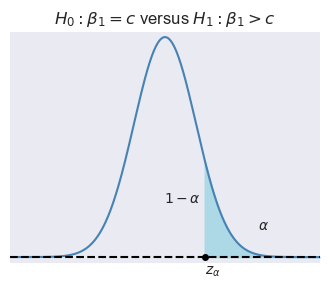
\includegraphics[width=3in,height=\textheight]{figures/critical_point1.png}

}

\subcaption{\label{fig-f12c1}Right-sided alternative hypothesis}

\end{minipage}%
%
\begin{minipage}{0.50\linewidth}

\centering{

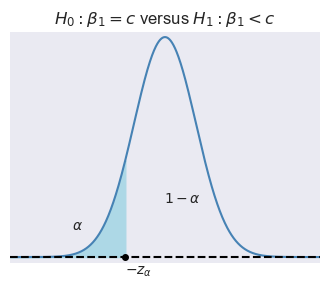
\includegraphics[width=3in,height=\textheight]{figures/critical_point2.png}

}

\subcaption{\label{fig-f12c2}Left-sided alternative hypothesis}

\end{minipage}%
\newline
\begin{minipage}{\linewidth}

\centering{

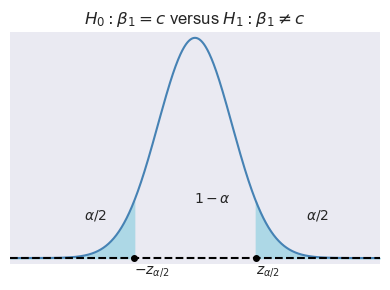
\includegraphics[width=3in,height=\textheight]{figures/critical_point3.png}

}

\subcaption{\label{fig-f12c3}Two-sided alternative hypothesis}

\end{minipage}%

\caption{\label{fig-critical_points}Rejection regions and critical
points}

\end{figure}%

\begin{example}[]\protect\hypertarget{exm-exm12-1}{}\label{exm-exm12-1}

Assume that \(\alpha=5\%\) and \(H_1:\beta_1\ne c\). Then, the critical
value on the left tail is the \(2.5\)th percentile of \(N(0,1)\), which
is \(-z_{\alpha/2}=-1.96\), and the critical value on the right tail is
the \(97.5\)th percentile of \(N(0,1)\), which is \(z_{\alpha/2}=1.96\).
In Python, we can compute these critical values as follows:

\begin{Shaded}
\begin{Highlighting}[]
\NormalTok{left\_critical }\OperatorTok{=}\NormalTok{ stats.norm.ppf(}\FloatTok{0.025}\NormalTok{, loc}\OperatorTok{=}\DecValTok{0}\NormalTok{, scale}\OperatorTok{=}\DecValTok{1}\NormalTok{)}
\NormalTok{right\_critical }\OperatorTok{=}\NormalTok{ stats.norm.ppf(}\FloatTok{0.975}\NormalTok{, loc}\OperatorTok{=}\DecValTok{0}\NormalTok{, scale}\OperatorTok{=}\DecValTok{1}\NormalTok{)}
\BuiltInTok{print}\NormalTok{(}\StringTok{"Left critical value:"}\NormalTok{, np.}\BuiltInTok{round}\NormalTok{(left\_critical, }\DecValTok{2}\NormalTok{))}
\BuiltInTok{print}\NormalTok{(}\StringTok{"Right critical value:"}\NormalTok{, np.}\BuiltInTok{round}\NormalTok{(right\_critical, }\DecValTok{2}\NormalTok{))}
\end{Highlighting}
\end{Shaded}

\begin{verbatim}
Left critical value: -1.96
Right critical value: 1.96
\end{verbatim}

\end{example}

Alternatively, we can compute the \(p\)-value to decide between \(H_0\)
and \(H_1\). The \textbf{\(p\)-value} is the probability of obtaining a
test statistic value that is more extreme than the actual one when
\(H_0\) is correct. Let \(t_{\text{calc}}\) be the realized value of the
\(t\)-statistic from Equation~\ref{eq-eq12-1}. Then, depending on the
type of alternative hypothesis, we can determine the \(p\)-value as \[
\begin{align}
\text{$p$-value}=
\begin{cases}
P_{H_0}\left(t > |t_{\text{calc}}|\right)=1-\Phi(|t_{\text{calc}}|)\,\,\text{for}\,\,H_1:\beta_1>c,\\
P_{H_0}\left(t <-|t_{\text{calc}}|\right)=\Phi(-|t_{\text{calc}}|)\,\,\text{for}\,\,H_1:\beta_1<c,\\
P_{H_0}\left(|t| > |t_{\text{calc}}|\right)=2\times\Phi(-|t_{\text{calc}}|)\,\,\text{for}\,H_1:\beta_1\ne c.
\end{cases}
\end{align}
\]

We reject \(H_0\) at the \(\alpha\%\) significance level if the
\(p\)-value is less than \(\alpha\); otherwise, we fail to reject
\(H_0\).

\begin{example}[]\protect\hypertarget{exm-exm12-2}{}\label{exm-exm12-2}

Assume that \(\alpha=0.05\) and the realized value of the
\(t\)-statistic is \(t_{\text{calc}}=-2.5\). Then, the \(p\)-value for
the two-sided alternative hypothesis is \[
\begin{align}
\text{$p$-value} = 2\times\Phi(-|-2.5|) = 2\times\Phi(-2.5).
\end{align}
\]

We can compute the \(p\)-value in Python as follows:

\begin{Shaded}
\begin{Highlighting}[]
\CommentTok{\# Compute p{-}value}
\NormalTok{t\_calc }\OperatorTok{=} \OperatorTok{{-}}\FloatTok{2.5}
\NormalTok{p\_value }\OperatorTok{=} \DecValTok{2} \OperatorTok{*}\NormalTok{ stats.norm.cdf(}\OperatorTok{{-}}\NormalTok{np.}\BuiltInTok{abs}\NormalTok{(t\_calc), loc}\OperatorTok{=}\DecValTok{0}\NormalTok{, scale}\OperatorTok{=}\DecValTok{1}\NormalTok{)}
\BuiltInTok{print}\NormalTok{(}\StringTok{"p{-}value:"}\NormalTok{, np.}\BuiltInTok{round}\NormalTok{(p\_value, }\DecValTok{4}\NormalTok{))}
\end{Highlighting}
\end{Shaded}

\begin{verbatim}
p-value: 0.0124
\end{verbatim}

Since \(p\text{-value} < 0.05\), we reject \(H_0\) at the \(5\%\)
significance level.

\end{example}

\begin{tcolorbox}[enhanced jigsaw, leftrule=.75mm, colbacktitle=quarto-callout-note-color!10!white, coltitle=black, toptitle=1mm, title={Key Concept 12.1: Testing \(H_0:\beta_1= c\) versus \(H_1:\beta_1\ne c\)}, breakable, left=2mm, toprule=.15mm, opacityback=0, titlerule=0mm, opacitybacktitle=0.6, bottomtitle=1mm, colback=white, arc=.35mm, colframe=quarto-callout-note-color-frame, rightrule=.15mm, bottomrule=.15mm]

\begin{itemize}
\tightlist
\item
  Compute the standard error of \(\hat{\beta}_1\),
  \(\SE(\hat{\beta}_{1})=\sqrt{\hat{\sigma}^2_{\hat{\beta}_1}}\).
\item
  Compute the \(t\)-statistic given in Equation~\ref{eq-eq12-1} under
  \(H_0\). Reject the nul hypothesis at the \(5\%\) significance level
  if \(|t|>1.96\).
\item
  Compute \(p\)-value from \(2\times\Phi(-|t_{\text{calc}}|)\), where
  \(t_{\text{calc}}\) is the actual test statistic computed in the
  second step. Reject the null hypothesis at the \(5\%\) significance
  level, if the \(p\)-value is less than \(0.05\).
\end{itemize}

\end{tcolorbox}

\section{Application to the test score
example}\label{application-to-the-test-score-example}

Recall that there are two options for running OLS regressions: (i) the
\texttt{smf.ols()} function and (ii) the \texttt{sm.OLS} function. In
the first option, \texttt{statsmodels} allows users to fit statistical
models using \texttt{R}-style formulas. We use the data set contained in
the \texttt{caschool.xlsx} file to estimate the following model: \[
\begin{align}
\text{TestScore}_i = \beta_0 + \beta_1 \text{STR}_i + u_i,
\end{align}
\]

In the data set, the test scores are denoted by \texttt{testscr} and the
student-teacher ratio by \texttt{str}.

\begin{Shaded}
\begin{Highlighting}[]
\CommentTok{\# Import data}
\NormalTok{CAschool }\OperatorTok{=}\NormalTok{ pd.read\_excel(}\StringTok{"data/caschool.xlsx"}\NormalTok{)}
\CommentTok{\# Column names}
\NormalTok{CAschool.columns}
\end{Highlighting}
\end{Shaded}

\begin{verbatim}
Index(['Observation Number', 'dist_cod', 'county', 'district', 'gr_span',
       'enrl_tot', 'teachers', 'calw_pct', 'meal_pct', 'computer', 'testscr',
       'comp_stu', 'expn_stu', 'str', 'avginc', 'el_pct', 'read_scr',
       'math_scr'],
      dtype='object')
\end{verbatim}

Consider \(H_0: \beta_1 = 0\) against \(H_1: \beta_1 \neq 0\). We use
the \texttt{smf.ols()} method to estimate the model.

\begin{Shaded}
\begin{Highlighting}[]
\CommentTok{\# Specify the model}
\NormalTok{model1 }\OperatorTok{=}\NormalTok{ smf.ols(formula}\OperatorTok{=}\StringTok{\textquotesingle{}testscr\textasciitilde{}str\textquotesingle{}}\NormalTok{,data}\OperatorTok{=}\NormalTok{CAschool)}
\CommentTok{\# Use the fit method to obtain parameter estimates}
\NormalTok{result1 }\OperatorTok{=}\NormalTok{ model1.fit()}
\CommentTok{\# Print the estimation results}
\BuiltInTok{print}\NormalTok{(result1.summary())}
\end{Highlighting}
\end{Shaded}

\begin{verbatim}
                            OLS Regression Results                            
==============================================================================
Dep. Variable:                testscr   R-squared:                       0.051
Model:                            OLS   Adj. R-squared:                  0.049
Method:                 Least Squares   F-statistic:                     22.58
Date:                Sun, 10 Aug 2025   Prob (F-statistic):           2.78e-06
Time:                        14:37:37   Log-Likelihood:                -1822.2
No. Observations:                 420   AIC:                             3648.
Df Residuals:                     418   BIC:                             3657.
Df Model:                           1                                         
Covariance Type:            nonrobust                                         
==============================================================================
                 coef    std err          t      P>|t|      [0.025      0.975]
------------------------------------------------------------------------------
Intercept    698.9330      9.467     73.825      0.000     680.323     717.543
str           -2.2798      0.480     -4.751      0.000      -3.223      -1.337
==============================================================================
Omnibus:                        5.390   Durbin-Watson:                   0.129
Prob(Omnibus):                  0.068   Jarque-Bera (JB):                3.589
Skew:                          -0.012   Prob(JB):                        0.166
Kurtosis:                       2.548   Cond. No.                         207.
==============================================================================

Notes:
[1] Standard Errors assume that the covariance matrix of the errors is correctly specified.
\end{verbatim}

Using the estimation results, we can compute \(t\)-statistic as \[
\begin{align}
t = \frac{\hat{\beta}_1-0}{SE(\hat{\beta}_1)} \approx \frac{-2.28}{0.48} \approx -4.75
\end{align}
\]

Note that the \texttt{result1.summary()} function also returns the
\(t\)-statistics. The column named \texttt{t} in the output includes the
\(t\)-statistics. Also note that we can return \(t\)-statistics through
the \texttt{result1.tvalues} attribute:

\begin{Shaded}
\begin{Highlighting}[]
\CommentTok{\# t{-}statistics}
\NormalTok{result1.tvalues}
\end{Highlighting}
\end{Shaded}

\begin{verbatim}
Intercept    73.824514
str          -4.751327
dtype: float64
\end{verbatim}

Assume that the significance level is \(\alpha = 0.05\). Then, the
corresponding critical value can be determined in the following way.

\begin{Shaded}
\begin{Highlighting}[]
\CommentTok{\# Critical value for 5 percent significance level}
\NormalTok{critical }\OperatorTok{=}\NormalTok{ stats.norm.ppf(}\FloatTok{0.975}\NormalTok{, loc}\OperatorTok{=}\DecValTok{0}\NormalTok{, scale}\OperatorTok{=}\DecValTok{1}\NormalTok{)}
\NormalTok{np.}\BuiltInTok{round}\NormalTok{(critical,}\DecValTok{2}\NormalTok{)}
\end{Highlighting}
\end{Shaded}

\begin{verbatim}
1.96
\end{verbatim}

Since \(|t| = |-4.75| = 4.75 > 1.96\), we reject \(H_0\) at the \(5\%\)
significance level. Thus, we say that \(\beta_1\) is statistically
significant at the \(5\%\) significance level.

The \(p\)-value for the two-sided alternative hypothesis is \[
\begin{align}
\text{p-value} = \text{Pr}_{H_0}\left(|t| > |t_{\text{calc}}|\right) = 2 \times \Phi(-|t_{\text{calc}}|),
\end{align}
\]

where \(t_{\text{calc}}\) is the actual \(t\)-statistic computed, which
is \(t\approx -4.75\). Then, we can compute the \(p\)-value in the
following way:

\begin{Shaded}
\begin{Highlighting}[]
\CommentTok{\# p{-}value for the two{-}sided alternative hypothesis}
\NormalTok{t }\OperatorTok{=}\NormalTok{ result1.tvalues[}\StringTok{"str"}\NormalTok{]}
\CommentTok{\# t=result1.tvalues.iloc[1]}
\NormalTok{p\_value }\OperatorTok{=} \DecValTok{2} \OperatorTok{*}\NormalTok{ stats.norm.cdf(}\OperatorTok{{-}}\NormalTok{np.}\BuiltInTok{abs}\NormalTok{(t), loc}\OperatorTok{=}\DecValTok{0}\NormalTok{, scale}\OperatorTok{=}\DecValTok{1}\NormalTok{)}
\NormalTok{p\_value}
\end{Highlighting}
\end{Shaded}

\begin{verbatim}
2.0208577446937873e-06
\end{verbatim}

Alternatively, we can return \(p\)-values through the
\texttt{result1.pvalues} attribute:

\begin{Shaded}
\begin{Highlighting}[]
\CommentTok{\# p{-}values}
\NormalTok{p\_value }\OperatorTok{=}\NormalTok{ result1.pvalues}
\NormalTok{p\_value}
\end{Highlighting}
\end{Shaded}

\begin{verbatim}
Intercept    6.569925e-242
str           2.783307e-06
dtype: float64
\end{verbatim}

Note that this value is slightly different from the one that we computed
above by
\texttt{p\_value\ =\ 2\ *\ stats.norm.cdf(-np.abs(t),\ loc=0,\ scale=1)}.
By default, the \texttt{model1.fit()} function uses the \(t\)
distribution for the computation. Thus, we need to use the t
distribution to get the same result:

\begin{Shaded}
\begin{Highlighting}[]
\NormalTok{t }\OperatorTok{=}\NormalTok{ result1.tvalues[}\StringTok{"str"}\NormalTok{]}
\CommentTok{\# t=result1.tvalues.iloc[1]}
\NormalTok{p\_value }\OperatorTok{=} \DecValTok{2} \OperatorTok{*}\NormalTok{ stats.t.cdf(}\OperatorTok{{-}}\NormalTok{np.}\BuiltInTok{abs}\NormalTok{(t), df}\OperatorTok{=}\DecValTok{418}\NormalTok{)}
\NormalTok{p\_value}
\end{Highlighting}
\end{Shaded}

\begin{verbatim}
2.783306521200329e-06
\end{verbatim}

Again, since \(p\text{-value} < 0.05\), we reject \(H_0\) at the \(5\%\)
significance level.

\section{Confidence intervals for a regression
parameter}\label{confidence-intervals-for-a-regression-parameter}

Recall that the \(95\%\) two-sided confidence interval can be
equivalently defined in the following ways:

\begin{itemize}
\tightlist
\item
  It is the set of points that cannot be rejected in a two-sided
  hypothesis testing problem with the \(5\%\) significance level.
\item
  It is a set-valued function of the data (an interval that is a
  function of the data) that contains the true parameter value \(95\%\)
  of the time in repeated samples.
\end{itemize}

Then, the \(95\%\) two-sided confidence interval for \(\beta_1\) refers
to the set of values for \(\beta_1\) such that
\(P\left(\{\beta_1:\left|\frac{\hat{\beta}_1-\beta_1}{SE(\hat{\beta}_1)}\right|\le 1.96\}\right) = 0.95\).
We can express the set
\(\{\beta_1:\left|\frac{\hat{\beta}_1-\beta_1}{SE(\hat{\beta}_1)}\right|\le 1.96\}\)
in a more convenient way: \[
\begin{align*}
&\{\beta_1:\left|\frac{\hat{\beta}_1-\beta_1}{\SE(\hat{\beta}_1)}\right|\le 1.96\}=\{\beta_1:-1.96\le \frac{\hat{\beta}_1-\beta_1}{\SE(\hat{\beta}_1)}\le 1.96\}\\
&=\{\beta_1:-\hat{\beta}_1-1.96\, \SE(\hat{\beta}_1)\le -\beta_1\le -\hat{\beta}_1+1.96\, \SE(\hat{\beta}_1)\}\\
&=\{\beta_1:\hat{\beta}_1 + 1.96 \, \SE(\hat{\beta}_1)\ge \beta_1\ge \hat{\beta}_1 -1.96\, \SE(\hat{\beta}_1)\}\\
&=\{\beta_1:\hat{\beta}_1 - 1.96 \, \SE(\hat{\beta}_1)\le \beta_1\le \hat{\beta}_1 +1.96\, \SE(\hat{\beta}_1)\}.
\end{align*}
\]

In our test score example, the \(95\%\) confidence interval is computed
in the following way:

\begin{Shaded}
\begin{Highlighting}[]
\CommentTok{\# Confidence interval for beta\_1}
\NormalTok{lower\_bound }\OperatorTok{=}\NormalTok{ result1.params[}\StringTok{"str"}\NormalTok{] }\OperatorTok{{-}}\NormalTok{ critical}\OperatorTok{*}\NormalTok{result1.bse[}\StringTok{"str"}\NormalTok{]}
\NormalTok{upper\_bound }\OperatorTok{=}\NormalTok{ result1.params[}\StringTok{"str"}\NormalTok{] }\OperatorTok{+}\NormalTok{ critical}\OperatorTok{*}\NormalTok{result1.bse[}\StringTok{"str"}\NormalTok{]}
\NormalTok{np.}\BuiltInTok{round}\NormalTok{([lower\_bound, upper\_bound], }\DecValTok{6}\NormalTok{)}
\end{Highlighting}
\end{Shaded}

\begin{verbatim}
array([-3.220249, -1.339367])
\end{verbatim}

Alternatively, we can resort to the \texttt{result1.conf\_int()} method
to return the confidence intervals for all parameters.

\begin{Shaded}
\begin{Highlighting}[]
\CommentTok{\# Confidence intervals for all parameters}
\NormalTok{result1.conf\_int(alpha}\OperatorTok{=}\FloatTok{0.05}\NormalTok{)}
\end{Highlighting}
\end{Shaded}

\begin{longtable}[]{@{}lll@{}}
\toprule\noalign{}
& 0 & 1 \\
\midrule\noalign{}
\endhead
\bottomrule\noalign{}
\endlastfoot
Intercept & 680.323126 & 717.542779 \\
str & -3.222980 & -1.336637 \\
\end{longtable}

Again note that these values are slightly different from the ones that
we computed above by \texttt{lower\_bound} and \texttt{upper\_bound}. By
default, the \texttt{model1.fit()} function uses the t distribution for
the computation instead of the normal distribution.

Note that the \(95\%\) two-sided confidence interval does not include
the hypothesized value in \(H_0:\beta_1=0\), and therefore, we reject
\(H_0\) at the \(5\%\) significance level.

\begin{tcolorbox}[enhanced jigsaw, leftrule=.75mm, colbacktitle=quarto-callout-note-color!10!white, coltitle=black, toptitle=1mm, title={Key Concept 12.2: Confidence Intervals for \(\beta_1\)}, breakable, left=2mm, toprule=.15mm, opacityback=0, titlerule=0mm, opacitybacktitle=0.6, bottomtitle=1mm, colback=white, arc=.35mm, colframe=quarto-callout-note-color-frame, rightrule=.15mm, bottomrule=.15mm]

The \(95\%\) two-sided confidence interval for \(\beta_1\) is an
interval that includes \(\beta_1\) in \(95\%\) of all possible random
samples. When the sample size is large, the two-sided confidence
intervals are as follows:

\begin{itemize}
\tightlist
\item
  The \(90\%\) two-sided confidence interval for \(\beta_1\) is
  \(\{\beta_1: \hat{\beta}_1 \pm 1.64 \times \text{SE}(\hat{\beta}_1)\}\).
\item
  The \(95\%\) two-sided confidence interval for \(\beta_1\) is
  \(\{\beta_1: \hat{\beta}_1 \pm 1.96 \times \text{SE}(\hat{\beta}_1)\}\).
\item
  The \(99\%\) two-sided confidence interval for \(\beta_1\) is
  \(\{\beta_1: \hat{\beta}_1 \pm 2.58\times \text{SE}(\hat{\beta}_1)\}\).
\end{itemize}

\end{tcolorbox}

\section{\texorpdfstring{Regression when \(X\) is a binary
variable}{Regression when X is a binary variable}}\label{regression-when-x-is-a-binary-variable}

In this section, we consider the following regression model: \[
\begin{align}
Y_i &= \beta_0 + \beta_1 D_i + u_i, \quad i = 1,2,\dots,n,
\end{align}
\]

where \(D_i\) is a dummy variable defined as \[
\begin{align*}
D_i &= \left\{\begin{array}{ll}
1, &\text{STR}_i < 20,\\
0, &\text{STR}_i \geq 20.
\end{array}\right.
\end{align*}
\] Under the least squares assumptions, if the student-teacher ratio is
high, i.e., \(D_i = 0\), then \(\E(Y_i|D_i = 0) = \beta_0\). However, if
the student-teacher ratio is low, i.e., \(D_i = 1\), then
\(\E(Y_i|D_i = 1) = \beta_0 + \beta_1\). Hence, \[
\begin{align*}
\E(Y_i|D_i = 1) - \E(Y_i|D_i = 0) &= \beta_0 + \beta_1 - \beta_0 = \beta_1.
\end{align*}
\]

That is, \(\beta_1\) gives the difference between the mean test score in
districts with low student-teacher ratios and the mean test score in
districts with high student-teacher ratios.

The dummy variable can be created by using a logical operator. The
command \texttt{mydata\$str\ \textless{}\ 20} will return \(1\) if
\(STR < 20\), otherwise \(0\).

\begin{Shaded}
\begin{Highlighting}[]
\CommentTok{\# Create the dummy variable D}
\NormalTok{CAschool[}\StringTok{"D"}\NormalTok{] }\OperatorTok{=}\NormalTok{ CAschool[}\StringTok{"str"}\NormalTok{] }\OperatorTok{\textless{}} \DecValTok{20}
\NormalTok{CAschool[[}\StringTok{"testscr"}\NormalTok{, }\StringTok{"str"}\NormalTok{, }\StringTok{"D"}\NormalTok{]].head()}
\end{Highlighting}
\end{Shaded}

\begin{longtable}[]{@{}llll@{}}
\toprule\noalign{}
& testscr & str & D \\
\midrule\noalign{}
\endhead
\bottomrule\noalign{}
\endlastfoot
0 & 690.799988 & 17.889910 & True \\
1 & 661.200012 & 21.524664 & False \\
2 & 643.599976 & 18.697226 & True \\
3 & 647.700012 & 17.357143 & True \\
4 & 640.849976 & 18.671329 & True \\
\end{longtable}

Figure~\ref{fig-fig12-2} shows the scatter plot of \texttt{TestScore}
and \texttt{D}. Since \texttt{D} takes only two values, namely \(0\) and
\(1\), we observe that the data points are clustered at \texttt{x=0} and
\texttt{x=1}. In Figure~\ref{fig-fig12-3}, we create a jittered version
of \texttt{D} by adding some random noise:
\texttt{jittered\_D\ =\ CAschool{[}\textquotesingle{}D\textquotesingle{}{]}\ +\ np.random.normal(0,\ 0.02,\ size=len(CAschool{[}\textquotesingle{}D\textquotesingle{}{]}))},
and construct a scatter plot between \texttt{TestScore} and
\texttt{jittered\_D}.

\begin{Shaded}
\begin{Highlighting}[]
\CommentTok{\# Scatterplot without jitter}
\NormalTok{sns.}\BuiltInTok{set}\NormalTok{(style}\OperatorTok{=}\StringTok{\textquotesingle{}darkgrid\textquotesingle{}}\NormalTok{)}
\NormalTok{fig, ax }\OperatorTok{=}\NormalTok{ plt.subplots(figsize}\OperatorTok{=}\NormalTok{(}\DecValTok{5}\NormalTok{, }\DecValTok{3}\NormalTok{))}
\NormalTok{ax.scatter(CAschool[}\StringTok{\textquotesingle{}D\textquotesingle{}}\NormalTok{], CAschool[}\StringTok{\textquotesingle{}testscr\textquotesingle{}}\NormalTok{], }
\NormalTok{            s}\OperatorTok{=}\FloatTok{1.5}\NormalTok{, c}\OperatorTok{=}\StringTok{\textquotesingle{}steelblue\textquotesingle{}}\NormalTok{, marker}\OperatorTok{=}\StringTok{\textquotesingle{}o\textquotesingle{}}\NormalTok{) }\CommentTok{\# s is for size, c for color, and marker for point shape}
\NormalTok{ax.set\_xlabel(}\StringTok{\textquotesingle{}D\textquotesingle{}}\NormalTok{)}
\NormalTok{ax.set\_ylabel(}\StringTok{\textquotesingle{}Test Score\textquotesingle{}}\NormalTok{)}
\NormalTok{plt.show()}
\end{Highlighting}
\end{Shaded}

\begin{figure}[H]

\centering{

\includegraphics{Chapter5-LinearRegressionOneRegressorInference_files/figure-pdf/fig-fig12-2-output-1.pdf}

}

\caption{\label{fig-fig12-2}Scatterplot of D and Test Score.}

\end{figure}%

\begin{Shaded}
\begin{Highlighting}[]
\CommentTok{\# Scatterplot with jitter}
\NormalTok{sns.}\BuiltInTok{set}\NormalTok{(style}\OperatorTok{=}\StringTok{\textquotesingle{}darkgrid\textquotesingle{}}\NormalTok{)}
\NormalTok{fig, ax }\OperatorTok{=}\NormalTok{ plt.subplots(figsize}\OperatorTok{=}\NormalTok{(}\DecValTok{5}\NormalTok{, }\DecValTok{3}\NormalTok{))}
\CommentTok{\# Add jitter to the dummy variable \textquotesingle{}D\textquotesingle{}}
\NormalTok{jittered\_D }\OperatorTok{=}\NormalTok{ CAschool[}\StringTok{\textquotesingle{}D\textquotesingle{}}\NormalTok{] }\OperatorTok{+}\NormalTok{ np.random.normal(}\DecValTok{0}\NormalTok{, }\FloatTok{0.02}\NormalTok{, size}\OperatorTok{=}\BuiltInTok{len}\NormalTok{(CAschool[}\StringTok{\textquotesingle{}D\textquotesingle{}}\NormalTok{])) }\CommentTok{\# Adjust the jitter scale as needed}
\CommentTok{\# Scatter plot with jitter}
\NormalTok{ax.scatter(jittered\_D, CAschool[}\StringTok{\textquotesingle{}testscr\textquotesingle{}}\NormalTok{], s}\OperatorTok{=}\DecValTok{4}\NormalTok{, c}\OperatorTok{=}\StringTok{\textquotesingle{}steelblue\textquotesingle{}}\NormalTok{, marker}\OperatorTok{=}\StringTok{\textquotesingle{}o\textquotesingle{}}\NormalTok{)}
\NormalTok{ax.set\_xlabel(}\StringTok{\textquotesingle{}D\textquotesingle{}}\NormalTok{)}
\NormalTok{ax.set\_ylabel(}\StringTok{\textquotesingle{}Test Score\textquotesingle{}}\NormalTok{)}
\NormalTok{plt.show()}
\end{Highlighting}
\end{Shaded}

\begin{figure}[H]

\centering{

\includegraphics{Chapter5-LinearRegressionOneRegressorInference_files/figure-pdf/fig-fig12-3-output-1.pdf}

}

\caption{\label{fig-fig12-3}Scatterplot of D and Test Score.}

\end{figure}%

As in the case of a continuous regressor, we can use the
\texttt{smf.ols()} function to estimate a dummy variable regression
model.

\begin{Shaded}
\begin{Highlighting}[]
\CommentTok{\# Specify the model}
\NormalTok{model2 }\OperatorTok{=}\NormalTok{ smf.ols(formula}\OperatorTok{=}\StringTok{\textquotesingle{}testscr \textasciitilde{} D\textquotesingle{}}\NormalTok{, data}\OperatorTok{=}\NormalTok{CAschool)}
\CommentTok{\# Use the fit method to obtain parameter estimates}
\NormalTok{result2 }\OperatorTok{=}\NormalTok{ model2.fit()}
\CommentTok{\# Print the estimation results}
\BuiltInTok{print}\NormalTok{(result2.summary())}
\end{Highlighting}
\end{Shaded}

\begin{verbatim}
                            OLS Regression Results                            
==============================================================================
Dep. Variable:                testscr   R-squared:                       0.037
Model:                            OLS   Adj. R-squared:                  0.035
Method:                 Least Squares   F-statistic:                     15.99
Date:                Sun, 10 Aug 2025   Prob (F-statistic):           7.52e-05
Time:                        14:37:37   Log-Likelihood:                -1825.4
No. Observations:                 420   AIC:                             3655.
Df Residuals:                     418   BIC:                             3663.
Df Model:                           1                                         
Covariance Type:            nonrobust                                         
==============================================================================
                 coef    std err          t      P>|t|      [0.025      0.975]
------------------------------------------------------------------------------
Intercept    649.9788      1.388    468.380      0.000     647.251     652.707
D[T.True]      7.3724      1.843      3.999      0.000       3.749      10.996
==============================================================================
Omnibus:                        3.061   Durbin-Watson:                   0.110
Prob(Omnibus):                  0.216   Jarque-Bera (JB):                2.448
Skew:                           0.052   Prob(JB):                        0.294
Kurtosis:                       2.641   Cond. No.                         2.81
==============================================================================

Notes:
[1] Standard Errors assume that the covariance matrix of the errors is correctly specified.
\end{verbatim}

The estimated regression function is \[
\begin{align}
\widehat{\text{TestScore}}_i = 649.98 + 7.38 D_i. 
\end{align}
\]

The estimate of \(\beta_1\) is \(7.38\), which indicates that students
in the districts with \texttt{STR\ \textless{}\ 20} have on average
\(7.38\) more points than students in other districts.

Figure~\ref{fig-fig12-4} shows the scatter plot along with the estimated
regression function. Since \(\beta_1=7.38\), the estimated regression
line is upward sloping, which indicates that the test scores are higher
in districts with low student-teacher ratios.

\begin{Shaded}
\begin{Highlighting}[]
\CommentTok{\# Set the style for seaborn}
\NormalTok{sns.set\_style(}\StringTok{\textquotesingle{}darkgrid\textquotesingle{}}\NormalTok{)}
\CommentTok{\# Create the figure and axis objects}
\NormalTok{fig, ax }\OperatorTok{=}\NormalTok{ plt.subplots(figsize}\OperatorTok{=}\NormalTok{(}\DecValTok{5}\NormalTok{, }\DecValTok{3}\NormalTok{))}
\CommentTok{\# Add jitter to the dummy variable \textquotesingle{}D\textquotesingle{}}
\NormalTok{jittered\_D }\OperatorTok{=}\NormalTok{ CAschool[}\StringTok{\textquotesingle{}D\textquotesingle{}}\NormalTok{] }\OperatorTok{+}\NormalTok{ np.random.normal(}\DecValTok{0}\NormalTok{, }\FloatTok{0.02}\NormalTok{, size}\OperatorTok{=}\BuiltInTok{len}\NormalTok{(CAschool[}\StringTok{\textquotesingle{}D\textquotesingle{}}\NormalTok{])) }\CommentTok{\# Adjust the jitter scale as needed}
\CommentTok{\# Scatter plot with jitter}
\NormalTok{ax.scatter(jittered\_D, CAschool[}\StringTok{\textquotesingle{}testscr\textquotesingle{}}\NormalTok{], s}\OperatorTok{=}\DecValTok{4}\NormalTok{, c}\OperatorTok{=}\StringTok{\textquotesingle{}steelblue\textquotesingle{}}\NormalTok{, marker}\OperatorTok{=}\StringTok{\textquotesingle{}o\textquotesingle{}}\NormalTok{)}
\CommentTok{\# Plot the regression line (without jitter)}
\NormalTok{ax.plot(CAschool[}\StringTok{\textquotesingle{}D\textquotesingle{}}\NormalTok{], result2.fittedvalues, color}\OperatorTok{=}\StringTok{\textquotesingle{}black\textquotesingle{}}\NormalTok{, linewidth}\OperatorTok{=}\DecValTok{1}\NormalTok{)}
\CommentTok{\# Set labels for axes}
\NormalTok{ax.set\_xlabel(}\StringTok{\textquotesingle{}D\textquotesingle{}}\NormalTok{)}
\NormalTok{ax.set\_ylabel(}\StringTok{\textquotesingle{}Test Score\textquotesingle{}}\NormalTok{)}
\CommentTok{\# Display the plot}
\NormalTok{plt.show()}
\end{Highlighting}
\end{Shaded}

\begin{figure}[H]

\centering{

\includegraphics{Chapter5-LinearRegressionOneRegressorInference_files/figure-pdf/fig-fig12-4-output-1.pdf}

}

\caption{\label{fig-fig12-4}The dummy variable regression model}

\end{figure}%

\section{Heteroskedasticity versus
Homoskedasticity}\label{heteroskedasticity-versus-homoskedasticity}

In the least squares assumptions introduced in Chapter 11, we only
assume the zero-conditional mean assumption about the error terms. Other
than this assumption, we do not impose any structure on the error term
\(u_i\). In this section, we introduce two concepts about the
conditional variance of the error term \(u_i\) given \(X_i\):
homoskedasticity and heteroskedasticity. We say that the error term
\(u_i\) is \textbf{homoskedastic} if the variance of \(u_i\) given
\(X_i\) is constant for all \(i = 1,2,\dots,n\). In particular, this
means that the variance does not depend on \(X_i\). On the other hand,
if the variance does depend on \(X_i\), we say that the error term
\(u_i\) is \textbf{heteroskedastic}.

Homoskedasticity and heteroskedasticity do not affect the unbiasedness
and consistency of the OLS estimators of \(\beta_0\) and \(\beta_1\).
However, they do affect the variance formulas of the OLS estimators
given in Theorem~\ref{thm-thm11.1} of Chapter 11. Under
homoskedasticity, let \(\var(u_i|X_i)=\sigma^2_u\), where \(\sigma^2_u\)
is an unknown scalar parameter. Then, the variance formulas of
\(\hat{\beta}_1\) and \(\hat{\beta}_0\) simplify to \[
\begin{align*}
&\sigma^2_{\widehat{\beta}_1} = \frac{1}{n}\frac{\var\left((X_i - \mu_X)u_i\right)}{\left(\var(X_i)\right)^2} = \frac{\sigma^2_u}{n\var(X_i)},\\
&\sigma^2_{\hat{\beta}_0} = \frac{1}{n}\frac{\var\left(H_i u_i\right)}{\left(\E(H_i^2)\right)^2} = \frac{\E(X^2_i)\sigma^2_u}{n\sigma^2_X}.
\end{align*}
\]

These variances are called the \textbf{homoskedasticity-only variances}.
They can be estimated as \[
\begin{align*}
&\hat{\sigma}^2_{\hat{\beta}_1} = \frac{\frac{1}{n-2}\sum_{i=1}^n \hat{u}_i^2}{\sum_{i=1}^n(X_i - \bar{X})^2},\\
&\hat{\sigma}^2_{\hat{\beta}_0}=\frac{\left(\frac{1}{n}\sum_{i=1}^nX^2_i\right)\left(\frac{1}{n-2}\sum_{i=1}^n \hat{u}_i^2\right)}{\frac{1}{n}\sum_{i=1}^n(X_i - \bar{X})^2}.
\end{align*}
\]

The \texttt{smf.ols()} function uses these formulas to compute the
standard errors, i.e., it only reports the homoskedasticity-only
standard errors. To get heteroskedasticity-robust standard errors, we
need to supply \texttt{cov\_type="HC1"} in the \texttt{fit} method, as
shown below.

\begin{Shaded}
\begin{Highlighting}[]
\CommentTok{\# Specify the model}
\NormalTok{model3 }\OperatorTok{=}\NormalTok{ smf.ols(formula}\OperatorTok{=}\StringTok{\textquotesingle{}testscr\textasciitilde{}str\textquotesingle{}}\NormalTok{, data}\OperatorTok{=}\NormalTok{CAschool)}
\CommentTok{\# Use the fit method to obtain parameter estimates}
\NormalTok{result3 }\OperatorTok{=}\NormalTok{ model3.fit(cov\_type}\OperatorTok{=}\StringTok{"HC1"}\NormalTok{)}
\CommentTok{\# Print the estimation results}
\BuiltInTok{print}\NormalTok{(result3.summary())}
\end{Highlighting}
\end{Shaded}

\begin{verbatim}
                            OLS Regression Results                            
==============================================================================
Dep. Variable:                testscr   R-squared:                       0.051
Model:                            OLS   Adj. R-squared:                  0.049
Method:                 Least Squares   F-statistic:                     19.26
Date:                Sun, 10 Aug 2025   Prob (F-statistic):           1.45e-05
Time:                        14:37:37   Log-Likelihood:                -1822.2
No. Observations:                 420   AIC:                             3648.
Df Residuals:                     418   BIC:                             3657.
Df Model:                           1                                         
Covariance Type:                  HC1                                         
==============================================================================
                 coef    std err          z      P>|z|      [0.025      0.975]
------------------------------------------------------------------------------
Intercept    698.9330     10.364     67.436      0.000     678.619     719.247
str           -2.2798      0.519     -4.389      0.000      -3.298      -1.262
==============================================================================
Omnibus:                        5.390   Durbin-Watson:                   0.129
Prob(Omnibus):                  0.068   Jarque-Bera (JB):                3.589
Skew:                          -0.012   Prob(JB):                        0.166
Kurtosis:                       2.548   Cond. No.                         207.
==============================================================================

Notes:
[1] Standard Errors are heteroscedasticity robust (HC1)
\end{verbatim}

In the following, we use the \texttt{summary\_col} function to present
results contained in \texttt{result1} and \texttt{result2} side by side.
The estimation results are presented in Table~\ref{tbl-t12-1}. The
estimation results in this table indicate that the
heteroskedasticity-robust standard errors are relatively large.

\begin{Shaded}
\begin{Highlighting}[]
\CommentTok{\# Print results in table form}
\NormalTok{models }\OperatorTok{=}\NormalTok{ [}\StringTok{\textquotesingle{}Homoskedastic Model\textquotesingle{}}\NormalTok{, }\StringTok{\textquotesingle{}Heteroskedastic Model\textquotesingle{}}\NormalTok{]}
\NormalTok{results\_table}\OperatorTok{=}\NormalTok{summary\_col(results}\OperatorTok{=}\NormalTok{[result1,result3],}
\NormalTok{                          float\_format}\OperatorTok{=}\StringTok{\textquotesingle{}}\SpecialCharTok{\%0.3f}\StringTok{\textquotesingle{}}\NormalTok{, }
\NormalTok{                          stars}\OperatorTok{=}\VariableTok{True}\NormalTok{,}
\NormalTok{                          model\_names}\OperatorTok{=}\NormalTok{models)}
\NormalTok{results\_table}
\end{Highlighting}
\end{Shaded}

\begin{figure}

\begin{minipage}{\linewidth}

\begin{table}[H]

\caption{\label{tbl-t12-1}The estimation results for the test scores
regressions}

\centering{

\caption{}
\label{}
\begin{center}
\begin{tabular}{lll}
\hline
               & Homoskedastic Model & Heteroskedastic Model  \\
\hline
Intercept      & 698.933***          & 698.933***             \\
               & (9.467)             & (10.364)               \\
str            & -2.280***           & -2.280***              \\
               & (0.480)             & (0.519)                \\
R-squared      & 0.051               & 0.051                  \\
R-squared Adj. & 0.049               & 0.049                  \\
\hline
\end{tabular}
\end{center}

}

\end{table}%

\end{minipage}%

\end{figure}%

\begin{tcolorbox}[enhanced jigsaw, leftrule=.75mm, colbacktitle=quarto-callout-note-color!10!white, coltitle=black, toptitle=1mm, title={Key Concept 12.3: Heteroskedasticity and Homoskedasticity}, breakable, left=2mm, toprule=.15mm, opacityback=0, titlerule=0mm, opacitybacktitle=0.6, bottomtitle=1mm, colback=white, arc=.35mm, colframe=quarto-callout-note-color-frame, rightrule=.15mm, bottomrule=.15mm]

\begin{itemize}
\tightlist
\item
  The error terms are said to be heteroskedastic if \(\var(u_i|X_i)\)
  depends on \(X_i\).
\item
  If \(\var(u_i|X_i)\) is constant, then the error terms are aid to be
  homoskedastic.
\item
  Regardless of whether the errors are homoskedastic or heteroskedastic,
  the OLS estimators of \(\beta_0\) and \(\beta_1\) remain unbiased,
  consistent, and asymptotically normal.
\item
  Heteroskedasticity and homoskedasticity only affect the variance
  formulas of the OLS estimators.
\end{itemize}

\end{tcolorbox}

In practice, which standard errors should we use? Stock and Watson
(2020) write that ``At a general level, economic theory rarely gives any
reason to believe that the errors are homoskedastic. It therefore is
prudent to assume that the errors might be heteroskedastic unless you
have compelling reasons to believe otherwise.'' Therefore, we recommend
using heteroskedasticity-robust standard errors in practice.

\section{The theoretical foundations of ordinary least
squares}\label{the-theoretical-foundations-of-ordinary-least-squares}

In this section, we consider the OLS estimator of \(\beta_1\) under the
following assumptions.

\begin{tcolorbox}[enhanced jigsaw, leftrule=.75mm, colbacktitle=quarto-callout-important-color!10!white, coltitle=black, toptitle=1mm, title={The Gauss--Markov Assumptions}, breakable, left=2mm, toprule=.15mm, opacityback=0, titlerule=0mm, opacitybacktitle=0.6, bottomtitle=1mm, colback=white, arc=.35mm, colframe=quarto-callout-important-color-frame, rightrule=.15mm, bottomrule=.15mm]

\begin{enumerate}
\def\labelenumi{\arabic{enumi}.}
\tightlist
\item
  The zero-conditional mean assumption: \(\E(u_i |X_i) = 0\).
\item
  The random sampling assumption: \((X_i, Y_i):\, i =1,2,\dots,n\) are
  independently and identically distributed (i.i.d.) across
  observations.
\item
  The no large outliers assumption: \(\E(X_i^4)<\infty\) and
  \(\E(Y_i^4)<\infty\).
\item
  The homoskedasticity assumption: \(\var(u_i|X_i)\) is constant for
  \(i =1,2,\dots,n\).
\end{enumerate}

\end{tcolorbox}

Under these extended assumptions, the following theorem justifies the
use of the OLS method.

\begin{theorem}[The Gauss-Markov Theorem for
\(\hat{\beta}_1\)]\protect\hypertarget{thm-thm12.1}{}\label{thm-thm12.1}

Under Gauss--Markov Assumption, the OLS estimator of \(\beta_1\) is the
best (most efficient) linear conditionally unbiased estimator (BLUE).

\end{theorem}

The proof of this theorem is given in Stock and Watson (2020). The
Gauss-Markov theorem states that the OLS estimator \(\hat{\beta}_1\) has
the smallest conditional variance among all conditionally unbiased
estimators that are linear functions of \(Y_1,\dots,Y_n\). There are two
limitations to this theorem. First, it requires the strong assumption
that error terms are homoskedastic, which mostly does not hold in
empirical applications. Second, there exist conditionally biased and
non-linear estimators that are more efficient than the OLS estimator. We
discuss such estimators in Chapter 21.

In the next chapter, we introduce the multiple linear regression model.
In Chapter 26, we extend the Gauss-Markov theorem to the multiple linear
regression model.

\chapter{Linear Regression with Multiple Regressors}\label{sec-multiple}

\begin{Shaded}
\begin{Highlighting}[]
\ImportTok{import}\NormalTok{ numpy }\ImportTok{as}\NormalTok{ np}
\ImportTok{import}\NormalTok{ pandas }\ImportTok{as}\NormalTok{ pd}
\ImportTok{import}\NormalTok{ matplotlib.pyplot }\ImportTok{as}\NormalTok{ plt}
\ImportTok{import}\NormalTok{ seaborn }\ImportTok{as}\NormalTok{ sns}
\ImportTok{import}\NormalTok{ statsmodels.api }\ImportTok{as}\NormalTok{ sm}
\ImportTok{import}\NormalTok{ statsmodels.formula.api }\ImportTok{as}\NormalTok{ smf}
\ImportTok{from}\NormalTok{ statsmodels.iolib.summary2 }\ImportTok{import}\NormalTok{ summary\_col}
\ImportTok{import}\NormalTok{ scipy.stats }\ImportTok{as}\NormalTok{ stats}
\ImportTok{from}\NormalTok{ mpl\_toolkits.mplot3d }\ImportTok{import}\NormalTok{ Axes3D}
\end{Highlighting}
\end{Shaded}

\[
\DeclareMathOperator{\cov}{cov}
\DeclareMathOperator{\corr}{corr} 
\DeclareMathOperator{\var}{var} 
\DeclareMathOperator{\SE}{SE} 
\DeclareMathOperator{\E}{E}
\DeclareMathOperator{\A}{\boldsymbol{A}}
\DeclareMathOperator{\x}{\boldsymbol{x}}
\DeclareMathOperator{\sgn}{sgn}  
\DeclareMathOperator{\argmin}{argmin} 
\newcommand{\tr}{\text{tr}}
\newcommand{\bs}{\boldsymbol}
\newcommand{\mb}{\mathbb}
\]

\section{Omitted variable bias}\label{omitted-variable-bias}

In a regression model of \(Y\) on \(X\), \textbf{omitted variable bias}
occurs if the regressor \(X\) is correlated with an omitted variable
that determines \(Y\). Let \(Z\) be a variable omitted from the
regression model. Then, \(Z\) causes omitted variable bias if \(Z\)
satisfies the following two conditions:

\begin{itemize}
\tightlist
\item
  \(Z\) is a determinant of \(Y\) (i.e., \(Z\) is part of \(u\)), and
\item
  \(Z\) is correlated with the regressor \(X\) (i.e.,
  corr\((Z,X)\ne0\)).
\end{itemize}

Under omitted variable bias, the zero conditional mean assumption
\(\E(u|X)=0\) fails because \(u\) contains a variable that is correlated
with \(X\). To see the effect of omitted variable bias on the OLS
estimator of \(\beta_1\), recall the following result from Chapter 11:
\[
\begin{align}
\hat{\beta}_1-\beta_1=\frac{\sum_{i=1}^n(X_i-\bar{X})u_i}{\sum_{i=1}^n(X_i-\bar{X})^2}.
\end{align}
\]

Under the second and the third least squares assumptions given in
Chapter 11, the law of large numbers ensure that
\(\frac{1}{n}\sum_{i=1}^n(X_i-\bar{X})^2\xrightarrow{p}\sigma^2_X\) and
\(\frac{1}{n}\sum_{i=1}^n(X_i-\bar{X})u_i\xrightarrow{p}\E\left[(X_i-\mu_X)u_i\right]=\text{cov}(X_i,u_i)=\sigma_{Xu}\).
Thus, we have \[
\begin{align}
\hat{\beta}_1-\beta_1=\frac{\sum_{i=1}^n(X_i-\bar{X})u_i}{\sum_{i=1}^n(X_i-\bar{X})^2}\xrightarrow{p}\frac{\sigma_{Xu}}{\sigma^2_X}=\frac{\sigma_u}{\sigma_X}\times\frac{\sigma_{Xu}}{\sigma_X\sigma_u}=\frac{\sigma_u}{\sigma_X}\times\rho_{Xu},
\end{align}
\] where \(\rho_{Xu}=\frac{\sigma_{Xu}}{\sigma_X\sigma_u}\) is the
correlation coefficient between \(X\) and \(u\). This results indicates
that the OLS estimator \(\hat{\beta}_1\) is inconsistent:
\begin{equation}\phantomsection\label{eq-eq13-1}{
\begin{align}
\hat{\beta}_1\xrightarrow{p}\beta_1+\frac{\sigma_u}{\sigma_X}\times\rho_{Xu}.
\end{align} 
}\end{equation}

\begin{tcolorbox}[enhanced jigsaw, leftrule=.75mm, colbacktitle=quarto-callout-note-color!10!white, coltitle=black, toptitle=1mm, title={Key Concept 13.1: Omitted Variable Bias}, breakable, left=2mm, toprule=.15mm, opacityback=0, titlerule=0mm, opacitybacktitle=0.6, bottomtitle=1mm, colback=white, arc=.35mm, colframe=quarto-callout-note-color-frame, rightrule=.15mm, bottomrule=.15mm]

If \(X\) is correlated with an omitted variable that affects \(Y\), then
the OLS estimator has omitted variable bias.

\begin{itemize}
\tightlist
\item
  Omitted variable causes the OLS estimator to be biased and
  inconsistent.
\item
  The bias is given by \(\frac{\sigma_u}{\sigma_X}\times\rho_{Xu}\) and
  does not vanish even when the sample size is large.
\item
  The sign and magnitude of bias depend on \(\rho_{Xu}\).
\end{itemize}

\end{tcolorbox}

\section{The multiple regression
model}\label{the-multiple-regression-model}

We can avoid omitted variable bias by extending the simple linear
regression model to the multiple linear regression model that includes
the omitted variable as an additional regressor. The multiple linear
regression model with \(k\) regressor is given by \[
\begin{align}
Y_i = \beta_0+\beta_1X_{1i}+\beta_2X_{2i}+\dots+\beta_kX_{ki}+u_i,\quad i=1,2,\dots,n,
\end{align}
\] where

\begin{itemize}
\tightlist
\item
  \(Y_i\) is the \(i\)th observation on the dependent variable \(Y\),
\item
  \((X_{1i},\dots,X_{ki})\) are the \(i\)th observations of the \(k\)
  regressors \((X_{1},\dots,X_{k})\),
\item
  \(\beta_0\) is the intercept parameter,
\item
  \(\beta_1,\dots,\beta_k\) are slope coefficients associated with
  \((X_{1},\dots,X_{k})\), and
\item
  \(u_i\) is the \(i\)th error term.
\end{itemize}

The population regression function is \[
\E(Y|X_{1},\dots,X_{k})=\beta_0+\beta_1X_{1}+\beta_2X_{2}+\dots+\beta_kX_{k}.
\]

The population regression function suggests that \(\beta_j\) gives the
effect of a unit change in \(X_j\) on the expected change in \(Y\),
holding other regressors constant. Using calculus, we have \[
\frac{\partial \E(Y|X_{1},\dots,X_{k})}{\partial X_j}=\beta_j,
\]

for \(j=1,\dots,k\). Therefore, \(\beta_j\) is also called the
\textbf{partial effect} of \(X_j\) on \(Y\), holding all other
regressors constant. In other words, after controlling for the effects
of the other regressors, \(\beta_j\) gives the effect of a unit change
in \(X_j\) on the expected value of \(Y\).

As in the case of the linear regression model with only one regressor,
we will only assume a zero-conditional mean assumption for the error
term \(u_i\). Also, the error term \(u_i\) is \textbf{homoskedastic} if
its conditional variance \(\var(u_i|X_{1i},\dots,X_{ki})\) is constant
for \(i=1,\dots,n\). Otherwise, the error term is said to be
\textbf{heteroskedastic}. As in the case of a linear regression model
with one regressor, homoskedasticity and heteroskedasticity only affect
the standard errors of the OLS estimator and do not affect the bias,
consistency, or asymptotic normality of the OLS estimator.

\section{The OLS estimators in multiple
regression}\label{the-ols-estimators-in-multiple-regression}

The OLS estimators are obtained by minimizing the sum of the squared
residuals (or prediction errors). Formally, the OLS estimators
\(\hat{\beta}_0,\dots,\hat{\beta}_k\) are the values of
\(b_0,\dots,b_k\) that minimize the following objective function: \[
\begin{align*}
\sum_{i=1}^n\left(Y_i-\left(b_0+b_1X_{1i}+b_2X_{2i}+\dots+b_kX_{ki}\right)\right)^2.
\end{align*}
\] The OLS estimator can be obtained using the matrix calculus. In
Chapter 26, we use matrix algebra to derive an explicit formula for the
OLS estimator.

The predicted values and residuals are defined similarly to the case of
a linear regression model with only one regressor:

\begin{itemize}
\tightlist
\item
  The predicted value of \(Y_i\) is
  \(\hat{Y}_i=\hat{\beta}_0+\hat{\beta}_1X_{1i}+\dots+\hat{\beta}_kX_{ki}\)
  for \(i=1,\dots,n\).
\item
  The \(i\)th residual is \(\hat{u}_i=Y_i-\hat{Y}_i\) for
  \(i=1,\dots,n\).
\end{itemize}

In the following theorem, we state an alternative way for computing the
OLS estimators.

\begin{theorem}[The Frisch--Waugh
Theorem]\protect\hypertarget{thm-thm13.0}{}\label{thm-thm13.0}

The OLS estimators \(\hat{\beta}_0, \dots, \hat{\beta}_k\) can
alternatively be computed through the following steps, involving a
sequence of shorter regressions:

\begin{enumerate}
\def\labelenumi{\arabic{enumi}.}
\tightlist
\item
  Run a regression of \(X_j\) on
  \(X_1, \dots, X_{j-1}, X_{j+1}, \dots, X_k\), including an intercept
  term. Let \(\tilde{X}_j\) be the residuals from this regression.
\item
  Run a regression of \(Y\) on
  \(X_1, \dots, X_{j-1}, X_{j+1}, \dots, X_k\), including an intercept
  term. Let \(\tilde{Y}\) be the residuals from this regression.
\item
  Finally, obtain the OLS estimator \(\hat{\beta}_j\) by running a
  regression of \(\tilde{Y}\) on \(\tilde{X}_j\), including an intercept
  term.
\end{enumerate}

\end{theorem}

The Frisch--Waugh theorem shows that by removing the variation
associated with \(X_1, \dots, X_{j-1}, X_{j+1}, \dots, X_k\) from both
\(X_j\) and \(Y\) through the regressions in Steps 1 and 2, the final
regression in Step 3 captures the effect of \(X_j\) on \(Y\) after
accounting for the influence of the other regressors.

\section{Application to test scores and the student--teacher
ratio}\label{application-to-test-scores-and-the-studentteacher-ratio}

We use the district-level test score data described in Chapter 11 to
estimate the following models: \[
\begin{align}
&\text{TestScore}_i = \beta_0 + \beta_1 \text{STR}_i + u_i,\\
&\text{TestScore}_i=\beta_0+\beta_1\times\text{STR}_i+\beta_2\times\text{PctEL}_i+u_i,
\end{align}
\] for \(i=1,\dots,420\), where \(\text{PctEL}_i\) is the percentage of
English learners in the \(i\)th district. We use the following code
chunks to import data from the \texttt{caschool.xlsx} file.

\begin{Shaded}
\begin{Highlighting}[]
\CommentTok{\# Import data}
\NormalTok{mydata }\OperatorTok{=}\NormalTok{ pd.read\_excel(}\StringTok{"data/caschool.xlsx"}\NormalTok{)}
\end{Highlighting}
\end{Shaded}

\begin{Shaded}
\begin{Highlighting}[]
\CommentTok{\# Column names}
\NormalTok{mydata.columns}
\end{Highlighting}
\end{Shaded}

\begin{verbatim}
Index(['Observation Number', 'dist_cod', 'county', 'district', 'gr_span',
       'enrl_tot', 'teachers', 'calw_pct', 'meal_pct', 'computer', 'testscr',
       'comp_stu', 'expn_stu', 'str', 'avginc', 'el_pct', 'read_scr',
       'math_scr'],
      dtype='object')
\end{verbatim}

The \texttt{describe} method can be used to get descriptive statistics
provided in Table~\ref{tbl-t13-1} on \texttt{str}, \texttt{el\_pct}, and
\texttt{testscr}.

\begin{Shaded}
\begin{Highlighting}[]
\CommentTok{\# Summary statistics}
\NormalTok{mydata[[}\StringTok{"str"}\NormalTok{, }\StringTok{"el\_pct"}\NormalTok{, }\StringTok{"testscr"}\NormalTok{]].}\BuiltInTok{round}\NormalTok{(}\DecValTok{3}\NormalTok{).describe().T}
\end{Highlighting}
\end{Shaded}

\begin{figure}

\begin{minipage}{\linewidth}

\begin{longtable}[]{@{}lllllllll@{}}

\caption{\label{tbl-t13-1}Summary statistics}

\tabularnewline

\toprule\noalign{}
& count & mean & std & min & 25\% & 50\% & 75\% & max \\
\midrule\noalign{}
\endhead
\bottomrule\noalign{}
\endlastfoot
str & 420.0 & 19.640417 & 1.891805 & 14.00 & 18.5825 & 19.723 & 20.87200
& 25.80 \\
el\_pct & 420.0 & 15.768152 & 18.285912 & 0.00 & 1.9410 & 8.778 &
22.96975 & 85.54 \\
testscr & 420.0 & 654.156548 & 19.053348 & 605.55 & 640.0500 & 654.450 &
666.66250 & 706.75 \\

\end{longtable}

\end{minipage}%

\end{figure}%

In Table~\ref{tbl-t13-2}, we provide sample correlation coefficients
between variables. We see that \texttt{PctEL} is negatively correlated
with \texttt{testscr} and positively correlated with \texttt{str}.

\begin{Shaded}
\begin{Highlighting}[]
\CommentTok{\# Correlation coefficients}
\NormalTok{mydata[[}\StringTok{"str"}\NormalTok{,}\StringTok{"el\_pct"}\NormalTok{, }\StringTok{"testscr"}\NormalTok{]].corr()}
\end{Highlighting}
\end{Shaded}

\begin{figure}

\begin{minipage}{\linewidth}

\begin{longtable}[]{@{}llll@{}}

\caption{\label{tbl-t13-2}The sample correlation coefficients}

\tabularnewline

\toprule\noalign{}
& str & el\_pct & testscr \\
\midrule\noalign{}
\endhead
\bottomrule\noalign{}
\endlastfoot
str & 1.000000 & 0.187642 & -0.226363 \\
el\_pct & 0.187642 & 1.000000 & -0.644124 \\
testscr & -0.226363 & -0.644124 & 1.000000 \\

\end{longtable}

\end{minipage}%

\end{figure}%

In the following code chunk, we use the \texttt{smf.ols()} function to
estimate both models.

\begin{Shaded}
\begin{Highlighting}[]
\CommentTok{\# Estimation}
\NormalTok{model1 }\OperatorTok{=}\NormalTok{ smf.ols(formula}\OperatorTok{=}\StringTok{\textquotesingle{}testscr\textasciitilde{}str\textquotesingle{}}\NormalTok{, data}\OperatorTok{=}\NormalTok{mydata)}
\NormalTok{result1 }\OperatorTok{=}\NormalTok{ model1.fit()}
\NormalTok{model2 }\OperatorTok{=}\NormalTok{ smf.ols(formula}\OperatorTok{=}\StringTok{\textquotesingle{}testscr\textasciitilde{}str+el\_pct\textquotesingle{}}\NormalTok{, data}\OperatorTok{=}\NormalTok{mydata)}
\NormalTok{result2 }\OperatorTok{=}\NormalTok{ model2.fit()}
\end{Highlighting}
\end{Shaded}

Using the \texttt{summary\_col()} function from the
\texttt{statsmodels.iolib.summary2}, we can present the estimation
results contained in \texttt{result1} and \texttt{result2} as shown in
Table~\ref{tbl-t13-3}.

\begin{Shaded}
\begin{Highlighting}[]
\CommentTok{\# Print results in table form}
\NormalTok{models }\OperatorTok{=}\NormalTok{ [}\StringTok{\textquotesingle{}Model 1\textquotesingle{}}\NormalTok{, }\StringTok{\textquotesingle{}Model 2\textquotesingle{}}\NormalTok{]}
\NormalTok{results\_table }\OperatorTok{=}\NormalTok{ summary\_col(results}\OperatorTok{=}\NormalTok{[result1, result2],}
\NormalTok{                            float\_format}\OperatorTok{=}\StringTok{\textquotesingle{}}\SpecialCharTok{\%0.3f}\StringTok{\textquotesingle{}}\NormalTok{, }
\NormalTok{                            stars}\OperatorTok{=}\VariableTok{True}\NormalTok{,}
\NormalTok{                            model\_names}\OperatorTok{=}\NormalTok{models)}
\NormalTok{results\_table}
\end{Highlighting}
\end{Shaded}

\begin{figure}

\begin{minipage}{\linewidth}

\begin{table}[H]

\caption{\label{tbl-t13-3}Estimation Results}

\centering{

\caption{}
\label{}
\begin{center}
\begin{tabular}{lll}
\hline
               & Model 1    & Model 2     \\
\hline
Intercept      & 698.933*** & 686.032***  \\
               & (9.467)    & (7.411)     \\
str            & -2.280***  & -1.101***   \\
               & (0.480)    & (0.380)     \\
el\_pct        &            & -0.650***   \\
               &            & (0.039)     \\
R-squared      & 0.051      & 0.426       \\
R-squared Adj. & 0.049      & 0.424       \\
\hline
\end{tabular}
\end{center}

}

\end{table}%

\end{minipage}%

\end{figure}%

Using the estimation results in Table~\ref{tbl-t13-3}, we can write the
estimated regression equations as \[
\begin{align*}
&\text{Model 1}: \widehat{TestScore}=698.9-2.280\times STR,\\
&\text{Model 2}: \widehat{TestScore}=686-1.10\times STR-0.65\times PctEL.
\end{align*}
\]

The estimate \(\hat{\beta}_1=-1.10\) in Model 2 indicates that when
\texttt{STR} increases by one student, the test score on average
declines by 1.10 points, holding \texttt{PctEL} constant. The estimate
\(\hat{\beta}_2=-0.65\) in Model 2 shows that one percent increase in
\texttt{PctEL} reduces the test score on average by \(0.65\) points,
holding \texttt{STR} constant. Note that the estimate
\(\hat{\beta}_1=-2.280\) in Model 1 is approximately twice as small as
the estimate \(\hat{\beta}_1=-1.10\) in Model 2, indicating that Model 1
suffers from omitted variable bias.

\section{Measures of fit}\label{measures-of-fit}

In this section, we provide four measures of fit for the multiple linear
regression model: (i) the standard error of the regression, (ii) the
root mean square errors, (ii) the regression \(R^2\), and (iv) the
adjusted \(R^2\).

The \textbf{standard error of the regression} (SER) is the estimator of
the standard deviation of the error term. It is calculated based on the
standard deviation of the residuals: \[
\text{SER} = s_{\hat{u}}=\sqrt{\frac{1}{n-k-1}\sum_{i=1}^n\hat{u}^2_i} = \sqrt{\frac{1}{n-k-1}SSR},
\]

where \(SSR\) is the sum of squared residuals
\(SSR=\sum_{i=1}^n\hat{u}^2_i\) and \(k\) is the number of regressors in
the model. The \textbf{root mean square errors} (RMSE) is defined by \[
RMSE = \sqrt{\frac{1}{n}SSR}.
\] Both SER and RMSE are measures of the spread of the distribution of
\(Y\) around the regression line. Equivalently, since
\(\hat{u}_i=Y_i-\hat{Y}_i\), we can interpret SER and RMSE as measures
of the spread of the distribution of the prediction errors. The smaller
the SER and RMSE, the better the fit of the regression model.

The \(R^2\) shows the fraction of the sample variance of \(Y\) explained
by the regressors. It is given by \[
\begin{align*}
R^2 = \frac{ESS}{TSS} = 1-\frac{SSR}{TSS},
\end{align*}
\]

where

\begin{itemize}
\tightlist
\item
  \(ESS=\sum_{i=1}^n\left(\hat{Y}_i-\bar{\hat{Y}}\right)^2\) is the
  explained sum of squares,
\item
  \(SSR=\sum_{i=1}^n\hat{u}^2_i\) is the sum of squared residuals, and
\item
  \(TSS=\sum_{i=1}^n\left(Y_i-\bar{Y}\right)^2\) is the total sum of
  squares.
\end{itemize}

In general, the SSR decreases when a new regressor is added to the
model, which leads to an increase in \(R^2\). However, this increase
does not necessarily indicate that the added variable improves the fit
of the model. The adjusted \(R^2\) (also denoted by \(\bar{R}^2\))
addresses this issue by penalizing the inclusion of additional
regressors. It is defined as \[
\begin{align*}
\bar{R}^2=1-\frac{n-1}{n-k-1}\times\frac{SSR}{TSS}=1-\frac{s^2_{\hat{u}}}{s^2_Y}.
\end{align*}
\]

Note that \(\bar{R}^2< R^2\), but if \(n\) is large, the two will be
very close because \((n-1)/(n-k-1)\) approaches one as \(n\) increases.
Also, adding a new regressor to the model affects \(\bar{R}^2\) in two
opposing directions. On the one hand, the new regressor decreases the
\(SSR\), which tends to increase \(\bar{R}^2\). On the other hand, the
factor \((n-1)(n-k-1)\) increases, which tends to reduce \(\bar{R}^2\).
Therefore, the net effect on \(\bar{R}^2\) depends on which of these two
effects is relatively larger.

The results in Table~\ref{tbl-t13-3} show that including \texttt{PctEL}
in the regression increases the \(R^2\) from \(0.051\) to \(0.426\).
Thus, including \texttt{PctEL} substantially improves the fit of the
regression. Because \(n\) is large and we have only two regressors, the
difference between \(R^2\) and \(\bar{R}^2\) is very small:
\(R^2 = 0.426\) vs.~\(\bar{R}^2 = 0.424\). Note that
Table~\ref{tbl-t13-3} does not include the SER measures. In the
following code chunk, we compute the SER measures for both models.

\begin{Shaded}
\begin{Highlighting}[]
\CommentTok{\# Computing SER for both models}
\NormalTok{SER1 }\OperatorTok{=}\NormalTok{ np.sqrt(np.}\BuiltInTok{sum}\NormalTok{(result1.resid}\OperatorTok{**}\DecValTok{2}\NormalTok{) }\OperatorTok{/}\NormalTok{ result1.df\_resid)}
\NormalTok{SER2 }\OperatorTok{=}\NormalTok{ np.sqrt(np.}\BuiltInTok{sum}\NormalTok{(result2.resid}\OperatorTok{**}\DecValTok{2}\NormalTok{) }\OperatorTok{/}\NormalTok{ result2.df\_resid)}
\CommentTok{\# Print the SER values}
\BuiltInTok{print}\NormalTok{(}\StringTok{"The SER for Model 1 is:"}\NormalTok{, np.}\BuiltInTok{round}\NormalTok{(SER1, }\DecValTok{1}\NormalTok{))}
\BuiltInTok{print}\NormalTok{(}\StringTok{"The SER for Model 2 is:"}\NormalTok{, np.}\BuiltInTok{round}\NormalTok{(SER2, }\DecValTok{1}\NormalTok{))}
\end{Highlighting}
\end{Shaded}

\begin{verbatim}
The SER for Model 1 is: 18.6
The SER for Model 2 is: 14.5
\end{verbatim}

The SER value \(18.6\) falls to \(14.5\) when \texttt{PctEL} is included
as a second regressor into the model. Finally, in the following code
chunk, we compute these measures of fit manually for the second model.
The results are given in Table~\ref{tbl-t13-t4}.

\begin{Shaded}
\begin{Highlighting}[]
\CommentTok{\# Computing SER, RMSE, R\^{}2, and adjusted R\^{}2 for the second model}
\NormalTok{n }\OperatorTok{=}\NormalTok{ result2.nobs}
\NormalTok{k }\OperatorTok{=}\NormalTok{ result2.k\_constant}
\NormalTok{y\_mean }\OperatorTok{=}\NormalTok{ np.mean(mydata[}\StringTok{"testscr"}\NormalTok{]) }\CommentTok{\# mean of avg. test{-}scores}

\NormalTok{SSR }\OperatorTok{=}\NormalTok{ np.}\BuiltInTok{sum}\NormalTok{(result2.resid}\OperatorTok{**}\DecValTok{2}\NormalTok{)}
\NormalTok{TSS }\OperatorTok{=}\NormalTok{ np.}\BuiltInTok{sum}\NormalTok{((mydata[}\StringTok{"testscr"}\NormalTok{] }\OperatorTok{{-}}\NormalTok{ y\_mean) }\OperatorTok{**} \DecValTok{2}\NormalTok{)}
\NormalTok{ESS }\OperatorTok{=}\NormalTok{ np.}\BuiltInTok{sum}\NormalTok{((result2.fittedvalues }\OperatorTok{{-}}\NormalTok{ y\_mean) }\OperatorTok{**} \DecValTok{2}\NormalTok{)}

\CommentTok{\# Compute measures}
\NormalTok{SER }\OperatorTok{=}\NormalTok{ np.sqrt(SSR}\OperatorTok{/}\NormalTok{(n }\OperatorTok{{-}}\NormalTok{ k }\OperatorTok{{-}} \DecValTok{1}\NormalTok{))}
\NormalTok{RMSE }\OperatorTok{=}\NormalTok{ np.sqrt(SSR}\OperatorTok{/}\NormalTok{n)}
\NormalTok{Rsq }\OperatorTok{=} \DecValTok{1} \OperatorTok{{-}}\NormalTok{ (SSR }\OperatorTok{/}\NormalTok{ TSS)}
\NormalTok{adj\_Rsq }\OperatorTok{=} \DecValTok{1} \OperatorTok{{-}}\NormalTok{ ((n }\OperatorTok{{-}} \DecValTok{1}\NormalTok{) }\OperatorTok{/}\NormalTok{ (n }\OperatorTok{{-}}\NormalTok{ k }\OperatorTok{{-}} \DecValTok{1}\NormalTok{)) }\OperatorTok{*}\NormalTok{ SSR }\OperatorTok{/}\NormalTok{ TSS}

\CommentTok{\# Print measures}
\NormalTok{fit\_measures }\OperatorTok{=}\NormalTok{ pd.DataFrame([SER, RMSE, Rsq, adj\_Rsq], }
\NormalTok{    index}\OperatorTok{=}\NormalTok{[}\StringTok{"SER"}\NormalTok{, }\StringTok{"RMSE"}\NormalTok{, }\StringTok{"R\^{}2"}\NormalTok{, }\StringTok{"Adj.R\^{}2"}\NormalTok{], }
\NormalTok{    columns}\OperatorTok{=}\NormalTok{[}\StringTok{""}\NormalTok{])}
\end{Highlighting}
\end{Shaded}

\begin{Shaded}
\begin{Highlighting}[]
\CommentTok{\# Print the measures of fit}
\NormalTok{fit\_measures}
\end{Highlighting}
\end{Shaded}

\begin{longtable}[]{@{}ll@{}}

\caption{\label{tbl-t13-t4}Measures of fit for the MLRM}

\tabularnewline

\toprule\noalign{}
& \\
\midrule\noalign{}
\endhead
\bottomrule\noalign{}
\endlastfoot
SER & 14.447173 \\
RMSE & 14.412734 \\
R\^{}2 & 0.426431 \\
Adj.R\^{}2 & 0.425059 \\

\end{longtable}

\section{The least squares assumptions for causal inference in multiple
regression}\label{the-least-squares-assumptions-for-causal-inference-in-multiple-regression}

In this section, we provide the least squares assumptions for the
multiple linear regression model. As in the case of the linear
regression model with one regressor, these assumptions ensure that the
OLS estimator has the desired properties. First, these assumptions
ensure that the OLS estimator is unbiased, consistent, and has an
asymptotic normal distribution. Second, under these assumptions, the OLS
estimates of the slope coefficients provide the estimated causal effects
of the regressors on the dependent variable. We list these assumptions
below.

\begin{tcolorbox}[enhanced jigsaw, leftrule=.75mm, colbacktitle=quarto-callout-important-color!10!white, coltitle=black, toptitle=1mm, title={The least squares assumptions for multiple regression}, breakable, left=2mm, toprule=.15mm, opacityback=0, titlerule=0mm, opacitybacktitle=0.6, bottomtitle=1mm, colback=white, arc=.35mm, colframe=quarto-callout-important-color-frame, rightrule=.15mm, bottomrule=.15mm]

\begin{enumerate}
\def\labelenumi{\arabic{enumi}.}
\tightlist
\item
  The zero-conditional mean assumption:
  \(\E\left(u_i|X_{1i},X_{i2},\dots,X_{ik}\right)=0\) for
  \(i=1,2,\dots,n\).
\item
  The random sampling assumption:
  \(\left(X_{1i},X_{i2},\dots,X_{ik},Y_i\right)\), \(i=1,2,\dots,n\),
  are i.i.d. draws from their joint distribution.
\item
  The no large outliers assumption: \(X_1,\dots, X_k\), and \(Y\) have
  finite fourth moments.
\item
  The multicollinearity assumption: There is no perfect
  multicollinearity.
\end{enumerate}

\end{tcolorbox}

The first assumption extends the zero-conditional mean assumption from
the linear regression model with one regressor to the model with
multiple regressors. We can use the correlation approach described in
Chapter 11 to check whether this assumption is violated. According to
this approach, in an empirical application, if we suspect that the error
term includes an omitted variable that is correlated with the included
regressors, then
\(\E\left(u_i | X_{1i}, X_{2i}, \dots, X_{ki}\right) \neq 0\). In
Section 13.8, we relax this assumption through a conditional mean
independence assumption for the variable of interest.

The second assumption requires that our sample data be collected through
simple random sampling. The third assumption stipulates that there are
no large outliers, which is ensured by requiring that both the dependent
variable and the regressors have finite fourth moments.

The fourth assumption is new and rules out perfect multicollinearity. In
a multiple linear regression model, \textbf{perfect multicollinearity}
arises if there is a perfect linear relationship among the regressors.
For example, the linear relationship such as \(X_1=0.5X_5+X_6\) suggests
perfect multicollinearity among the regressors \(X_1\), \(X_5\), and
\(X_6\). In Chapter 26, we show that the OLS estimator is not defined
when perfect multicollinearity is present.

Theorem~\ref{thm-thm13-1} summarizes the properties of the OLS
estimators under these four assumptions. In this theorem, we do not
provide explicit formulas for the asymptotic variance of the OLS
estimators. In Chapter 26, we use linear algebra to derive these
formulas.

\begin{theorem}[Properties of OLS
Estimators]\protect\hypertarget{thm-thm13-1}{}\label{thm-thm13-1}

Under the four least squares assumptions, we have
\(\E(\hat{\beta}_j) = \beta_j\) for \(j=1,\dots,k\), i.e, the OLS
estimators are \textbf{unbiased}. As \(n\to\infty\),
\(\hat{\beta}_0,\dots,\hat{\beta}_k\) are consistent and have a joint
multivariate normal distribution.

\end{theorem}

According to Theorem~\ref{thm-thm13-1}, the OLS estimators
\(\hat{\beta}_0, \dots, \hat{\beta}_k\) satisfy three properties: (i)
unbiasedness, (ii) consistency, and (iii) asymptotic joint normality. In
the following simulation study, we use simulated data to show that these
properties hold when \(n\) is large enough. We assume that the dependent
variable is generated according too \[
Y_i = \beta_0+\beta_1X_{1i}+\beta_2X_{2i}+u_i,
\] where \(\beta_0=0.5\), \(\beta_1=1.5\), \(\beta_2=1\) and
\(u_i\sim t_3\). For the regressors, we assume that they are generated
from the following bivariate normal distribution: \[
(X_{1i},X_{2i})^{'}\sim N\left(\begin{pmatrix}2\\1.5\end{pmatrix},
\begin{pmatrix}
5&1.5\\
1.5&5
\end{pmatrix}
\right).
\]

We set the sample size \(n\) to 100 and generate 10000 samples. Using
each sample, we estimate the model and store the estimated coefficients
in the \texttt{coefs} array. We then generate histograms and density
plots for each estimated coefficient. We provide the simulation results
in Figure~\ref{fig-fig13-1}. The histograms and density plots for
\(\hat{\beta}_0\), \(\hat{\beta}_1\), and \(\hat{\beta}_2\) are
bell-shaped and centered around the respective true parameter values.
The surface plot in Figure~\ref{fig-fig13-1} resembles that of a
bivariate normal distribution, suggesting that \(\hat{\beta}_1\) and
\(\hat{\beta}_2\) have a joint bivariate normal distribution.

\begin{Shaded}
\begin{Highlighting}[]
\CommentTok{\# Set sample size and number of simulations}
\NormalTok{n }\OperatorTok{=} \DecValTok{100}
\NormalTok{n\_simulations }\OperatorTok{=} \DecValTok{10000}

\CommentTok{\# Initialize array for coefficients}
\NormalTok{coefs }\OperatorTok{=}\NormalTok{ np.zeros((n\_simulations, }\DecValTok{3}\NormalTok{))}

\CommentTok{\# Set seed for reproducibility}
\NormalTok{np.random.seed(}\DecValTok{15}\NormalTok{)}

\CommentTok{\# Loop for sampling and estimation}
\ControlFlowTok{for}\NormalTok{ i }\KeywordTok{in} \BuiltInTok{range}\NormalTok{(n\_simulations):}
    \CommentTok{\# Generate multivariate normal samples}
\NormalTok{    mean }\OperatorTok{=}\NormalTok{ [}\DecValTok{2}\NormalTok{, }\FloatTok{1.5}\NormalTok{]}
\NormalTok{    cov }\OperatorTok{=}\NormalTok{ [[}\DecValTok{5}\NormalTok{, }\FloatTok{1.5}\NormalTok{], [}\FloatTok{1.5}\NormalTok{, }\DecValTok{5}\NormalTok{]]}
\NormalTok{    X }\OperatorTok{=}\NormalTok{ stats.multivariate\_normal.rvs(mean}\OperatorTok{=}\NormalTok{mean, cov}\OperatorTok{=}\NormalTok{cov, size}\OperatorTok{=}\NormalTok{n)}
    
    \CommentTok{\# Generate random errors}
\NormalTok{    u }\OperatorTok{=}\NormalTok{ np.random.standard\_t(df}\OperatorTok{=}\DecValTok{3}\NormalTok{,size}\OperatorTok{=}\NormalTok{n)}
    
    \CommentTok{\# Generate dependent variable}
\NormalTok{    Y }\OperatorTok{=} \FloatTok{0.5} \OperatorTok{+} \FloatTok{1.5} \OperatorTok{*}\NormalTok{ X[:, }\DecValTok{0}\NormalTok{] }\OperatorTok{+} \DecValTok{1} \OperatorTok{*}\NormalTok{ X[:, }\DecValTok{1}\NormalTok{] }\OperatorTok{+}\NormalTok{ u}
    
    \CommentTok{\# Fit linear regression using statsmodels}
\NormalTok{    X\_with\_const }\OperatorTok{=}\NormalTok{ sm.add\_constant(X) }\CommentTok{\# Add constant term for intercept}
\NormalTok{    model }\OperatorTok{=}\NormalTok{ sm.OLS(Y, X\_with\_const).fit()}
\NormalTok{    coefs[i, :] }\OperatorTok{=}\NormalTok{ model.params }\CommentTok{\# Store the coefficients}
\end{Highlighting}
\end{Shaded}

\begin{Shaded}
\begin{Highlighting}[]
\CommentTok{\# Simulation results}
\CommentTok{\# Set seaborn style}
\NormalTok{sns.}\BuiltInTok{set}\NormalTok{(style}\OperatorTok{=}\StringTok{\textquotesingle{}darkgrid\textquotesingle{}}\NormalTok{)}

\CommentTok{\# Create the figure}
\NormalTok{fig }\OperatorTok{=}\NormalTok{ plt.figure(figsize}\OperatorTok{=}\NormalTok{(}\DecValTok{8}\NormalTok{, }\DecValTok{7}\NormalTok{))}

\CommentTok{\# Histogram and density plot for beta\_0}
\NormalTok{ax1 }\OperatorTok{=}\NormalTok{ fig.add\_subplot(}\DecValTok{221}\NormalTok{)}
\NormalTok{sns.histplot(coefs[:, }\DecValTok{0}\NormalTok{], bins}\OperatorTok{=}\DecValTok{50}\NormalTok{, kde}\OperatorTok{=}\VariableTok{True}\NormalTok{, color}\OperatorTok{=}\StringTok{\textquotesingle{}steelblue\textquotesingle{}}\NormalTok{, stat}\OperatorTok{=}\StringTok{\textquotesingle{}density\textquotesingle{}}\NormalTok{, ax}\OperatorTok{=}\NormalTok{ax1, alpha}\OperatorTok{=}\FloatTok{0.6}\NormalTok{)}
\NormalTok{ax1.axvline(np.mean(coefs[:, }\DecValTok{0}\NormalTok{]), color}\OperatorTok{=}\StringTok{\textquotesingle{}black\textquotesingle{}}\NormalTok{, linestyle}\OperatorTok{=}\StringTok{\textquotesingle{}dashed\textquotesingle{}}\NormalTok{, linewidth}\OperatorTok{=}\DecValTok{1}\NormalTok{, label}\OperatorTok{=}\StringTok{\textquotesingle{}Mean\textquotesingle{}}\NormalTok{)}
\NormalTok{ax1.set\_xlabel(}\VerbatimStringTok{r\textquotesingle{}$\textbackslash{}hat\{\textbackslash{}beta\}\_0$\textquotesingle{}}\NormalTok{, fontsize}\OperatorTok{=}\DecValTok{12}\NormalTok{)}
\NormalTok{ax1.set\_ylabel(}\StringTok{\textquotesingle{}Density\textquotesingle{}}\NormalTok{, fontsize}\OperatorTok{=}\DecValTok{12}\NormalTok{)}
\NormalTok{ax1.legend(frameon}\OperatorTok{=}\VariableTok{False}\NormalTok{)}
\NormalTok{ax1.set\_xlim(}\OperatorTok{{-}}\FloatTok{0.5}\NormalTok{,}\FloatTok{1.5}\NormalTok{)}

\CommentTok{\# Histogram and density plot for beta\_1}
\NormalTok{ax2 }\OperatorTok{=}\NormalTok{ fig.add\_subplot(}\DecValTok{222}\NormalTok{)}
\NormalTok{sns.histplot(coefs[:, }\DecValTok{1}\NormalTok{], bins}\OperatorTok{=}\DecValTok{50}\NormalTok{, kde}\OperatorTok{=}\VariableTok{True}\NormalTok{, color}\OperatorTok{=}\StringTok{\textquotesingle{}steelblue\textquotesingle{}}\NormalTok{, stat}\OperatorTok{=}\StringTok{\textquotesingle{}density\textquotesingle{}}\NormalTok{, ax}\OperatorTok{=}\NormalTok{ax2, alpha}\OperatorTok{=}\FloatTok{0.6}\NormalTok{)}
\NormalTok{ax2.axvline(np.mean(coefs[:, }\DecValTok{1}\NormalTok{]), color}\OperatorTok{=}\StringTok{\textquotesingle{}black\textquotesingle{}}\NormalTok{, linestyle}\OperatorTok{=}\StringTok{\textquotesingle{}dashed\textquotesingle{}}\NormalTok{, linewidth}\OperatorTok{=}\DecValTok{1}\NormalTok{, label}\OperatorTok{=}\StringTok{\textquotesingle{}Mean\textquotesingle{}}\NormalTok{)}
\NormalTok{ax2.set\_xlabel(}\VerbatimStringTok{r\textquotesingle{}$\textbackslash{}hat\{\textbackslash{}beta\}\_1$\textquotesingle{}}\NormalTok{, fontsize}\OperatorTok{=}\DecValTok{12}\NormalTok{)}
\NormalTok{ax2.set\_ylabel(}\StringTok{\textquotesingle{}Density\textquotesingle{}}\NormalTok{, fontsize}\OperatorTok{=}\DecValTok{12}\NormalTok{)}
\NormalTok{ax2.legend(frameon}\OperatorTok{=}\VariableTok{False}\NormalTok{)}
\NormalTok{ax2.set\_xlim(}\FloatTok{1.2}\NormalTok{,}\FloatTok{1.8}\NormalTok{)}

\CommentTok{\# Histogram and density plot for beta\_2}
\NormalTok{ax3 }\OperatorTok{=}\NormalTok{ fig.add\_subplot(}\DecValTok{223}\NormalTok{)}
\NormalTok{sns.histplot(coefs[:, }\DecValTok{2}\NormalTok{], bins}\OperatorTok{=}\DecValTok{50}\NormalTok{, kde}\OperatorTok{=}\VariableTok{True}\NormalTok{, color}\OperatorTok{=}\StringTok{\textquotesingle{}steelblue\textquotesingle{}}\NormalTok{, stat}\OperatorTok{=}\StringTok{\textquotesingle{}density\textquotesingle{}}\NormalTok{, ax}\OperatorTok{=}\NormalTok{ax3, alpha}\OperatorTok{=}\FloatTok{0.6}\NormalTok{)}
\NormalTok{ax3.axvline(np.mean(coefs[:, }\DecValTok{2}\NormalTok{]), color}\OperatorTok{=}\StringTok{\textquotesingle{}black\textquotesingle{}}\NormalTok{, linestyle}\OperatorTok{=}\StringTok{\textquotesingle{}dashed\textquotesingle{}}\NormalTok{, linewidth}\OperatorTok{=}\DecValTok{1}\NormalTok{, label}\OperatorTok{=}\StringTok{\textquotesingle{}Mean\textquotesingle{}}\NormalTok{)}
\NormalTok{ax3.set\_xlabel(}\VerbatimStringTok{r\textquotesingle{}$\textbackslash{}hat\{\textbackslash{}beta\}\_2$\textquotesingle{}}\NormalTok{, fontsize}\OperatorTok{=}\DecValTok{12}\NormalTok{)}
\NormalTok{ax3.set\_ylabel(}\StringTok{\textquotesingle{}Density\textquotesingle{}}\NormalTok{, fontsize}\OperatorTok{=}\DecValTok{12}\NormalTok{)}
\NormalTok{ax3.set\_xlim(}\FloatTok{0.6}\NormalTok{,}\FloatTok{1.4}\NormalTok{)}
\NormalTok{ax3.legend(frameon}\OperatorTok{=}\VariableTok{False}\NormalTok{)}

\CommentTok{\# Kernel density estimation for beta\_1 and beta\_2}
\NormalTok{kde }\OperatorTok{=}\NormalTok{ stats.gaussian\_kde(coefs[:, }\DecValTok{1}\NormalTok{:].T)}

\CommentTok{\# Create grid for 3D plot}
\NormalTok{x\_grid }\OperatorTok{=}\NormalTok{ np.linspace(}\FloatTok{1.2}\NormalTok{, }\FloatTok{1.8}\NormalTok{, }\DecValTok{100}\NormalTok{)}
\NormalTok{y\_grid }\OperatorTok{=}\NormalTok{ np.linspace(}\FloatTok{0.6}\NormalTok{, }\FloatTok{1.4}\NormalTok{, }\DecValTok{100}\NormalTok{)}
\NormalTok{X\_grid, Y\_grid }\OperatorTok{=}\NormalTok{ np.meshgrid(x\_grid, y\_grid)}
\NormalTok{Z\_grid }\OperatorTok{=}\NormalTok{ kde(np.vstack([X\_grid.ravel(), Y\_grid.ravel()])).reshape(X\_grid.shape)}

\CommentTok{\# 3D density estimate plot for beta\_1 and beta\_2}
\NormalTok{ax4 }\OperatorTok{=}\NormalTok{ fig.add\_subplot(}\DecValTok{224}\NormalTok{, projection}\OperatorTok{=}\StringTok{\textquotesingle{}3d\textquotesingle{}}\NormalTok{)}
\NormalTok{surf }\OperatorTok{=}\NormalTok{ ax4.plot\_surface(X\_grid, Y\_grid, Z\_grid, cmap}\OperatorTok{=}\StringTok{\textquotesingle{}coolwarm\textquotesingle{}}\NormalTok{, edgecolor}\OperatorTok{=}\StringTok{\textquotesingle{}none\textquotesingle{}}\NormalTok{, rstride}\OperatorTok{=}\DecValTok{1}\NormalTok{, cstride}\OperatorTok{=}\DecValTok{1}\NormalTok{, alpha}\OperatorTok{=}\FloatTok{0.85}\NormalTok{)}
\NormalTok{ax4.contour(X\_grid, Y\_grid, Z\_grid, zdir}\OperatorTok{=}\StringTok{\textquotesingle{}z\textquotesingle{}}\NormalTok{, offset}\OperatorTok{=}\NormalTok{np.}\BuiltInTok{min}\NormalTok{(Z\_grid), cmap}\OperatorTok{=}\StringTok{\textquotesingle{}coolwarm\textquotesingle{}}\NormalTok{, linestyles}\OperatorTok{=}\StringTok{"solid"}\NormalTok{)}
\NormalTok{ax4.set\_xlabel(}\VerbatimStringTok{r\textquotesingle{}$\textbackslash{}hat\{\textbackslash{}beta\}\_1$\textquotesingle{}}\NormalTok{, fontsize}\OperatorTok{=}\DecValTok{12}\NormalTok{)}
\NormalTok{ax4.set\_ylabel(}\VerbatimStringTok{r\textquotesingle{}$\textbackslash{}hat\{\textbackslash{}beta\}\_2$\textquotesingle{}}\NormalTok{, fontsize}\OperatorTok{=}\DecValTok{12}\NormalTok{)}
\CommentTok{\#ax4.set\_zlabel(\textquotesingle{}Estimated Density\textquotesingle{}, fontsize=12)}

\CommentTok{\# Add color bar for surface}
\NormalTok{fig.colorbar(surf, ax}\OperatorTok{=}\NormalTok{ax4, shrink}\OperatorTok{=}\FloatTok{0.5}\NormalTok{, aspect}\OperatorTok{=}\DecValTok{10}\NormalTok{)}

\CommentTok{\# Remove ticks from 3D plot}
\NormalTok{ax4.set\_xticks([])}
\NormalTok{ax4.set\_yticks([])}
\NormalTok{ax4.set\_zticks([])}

\CommentTok{\# Set a different viewing angle for better perspective}
\NormalTok{ax4.view\_init(elev}\OperatorTok{=}\DecValTok{30}\NormalTok{, azim}\OperatorTok{=}\DecValTok{220}\NormalTok{)}

\CommentTok{\# Adjust layout for better spacing}
\NormalTok{plt.tight\_layout()}
\NormalTok{plt.show()}
\end{Highlighting}
\end{Shaded}

\begin{figure}[H]

\centering{

\includegraphics{Chapter6-MultipleRegression_files/figure-pdf/fig-fig13-1-output-1.pdf}

}

\caption{\label{fig-fig13-1}Histogram and density plots of the
simulation results}

\end{figure}%

\section{Multicollinearity}\label{multicollinearity}

When there is an exact linear relationship between regressors, we say
there is perfect multicollinearity. On the other hand, when two or more
regressors are highly correlated but not perfectly, we say that there is
imperfect multicollinearity. Although imperfect multicollinearity does
not violate the least squares assumptions, it can result in large
standard errors for one or more of the OLS estimators.

The perfect multicollinearity among the dummy variables is called the
\textbf{dummy variable trap}. To illustrate the dummy variable trap, we
use the data set contained in the \texttt{ch8\_cps.xlsx} file. This data
set includes the following variables.

\begin{itemize}
\tightlist
\item
  \texttt{Female}: 1 if female; 0 if male
\item
  \texttt{Age}: Age (in Years)
\item
  \texttt{Ahe}: Average Hourly Earnings in 2015
\item
  \texttt{Yrseduc}: Years of Education
\item
  \texttt{Northeast}: 1 if from the Northeast, 0 otherwise
\item
  \texttt{Midwest}: 1 if from the Midwest, 0 otherwise
\item
  \texttt{South}: 1 if from the South, 0 otherwise
\item
  \texttt{West}: 1 if from the West, 0 otherwise
\end{itemize}

Note that there are four regional dummy variables, denoted by
\texttt{Northeast}, \texttt{Midwest}, \texttt{South}, and \texttt{West}.
We consider the following regression model: \[
\begin{align*}
\text{Ahe}&=\beta_0+\beta_1\text{Yrseduc}+\beta_2\text{Female}+\beta_3\text{Northeast}\\
&+\beta_4\text{Midwest}+\beta_5\text{South}+\beta_6\text{West}+u.
\end{align*}
\]

This regression suffers from the dummy variable trap beacuse we have a
perfect linear relationship among the regional dummy variables: \[
\text{Northeast}+\text{Midwest}+\text{South}+\text{West}=1.
\]

To resolve this, we will treat the last dummy variable as the
\textbf{base category} and exclude it from the regression model.

We use the following code chunks to import the data.
Table~\ref{tbl-t13-5} provides summary statistics.

\begin{Shaded}
\begin{Highlighting}[]
\CommentTok{\# Import data}
\NormalTok{mydata }\OperatorTok{=}\NormalTok{ pd.read\_excel(}\StringTok{"data/ch8\_cps.xlsx"}\NormalTok{)}
\CommentTok{\# Display column names}
\NormalTok{mydata.columns}
\end{Highlighting}
\end{Shaded}

\begin{verbatim}
Index(['ahe', 'yrseduc', 'female', 'age', 'northeast', 'midwest', 'south',
       'west'],
      dtype='object')
\end{verbatim}

\begin{Shaded}
\begin{Highlighting}[]
\CommentTok{\# Summary statistics}
\NormalTok{mydata.}\BuiltInTok{round}\NormalTok{(}\DecValTok{3}\NormalTok{).describe().T}
\end{Highlighting}
\end{Shaded}

\begin{figure}

\begin{minipage}{\linewidth}

\begin{longtable}[]{@{}lllllllll@{}}

\caption{\label{tbl-t13-5}Summary statistics}

\tabularnewline

\toprule\noalign{}
& count & mean & std & min & 25\% & 50\% & 75\% & max \\
\midrule\noalign{}
\endhead
\bottomrule\noalign{}
\endlastfoot
ahe & 59668.0 & 25.213725 & 17.288965 & 2.0 & 13.736 & 20.192 & 31.25 &
228.365 \\
yrseduc & 59668.0 & 14.094389 & 2.598457 & 6.0 & 12.000 & 13.000 & 16.00
& 20.000 \\
female & 59668.0 & 0.438510 & 0.496209 & 0.0 & 0.000 & 0.000 & 1.00 &
1.000 \\
age & 59668.0 & 42.884846 & 12.583984 & 15.0 & 33.000 & 42.000 & 52.00 &
85.000 \\
northeast & 59668.0 & 0.157371 & 0.364153 & 0.0 & 0.000 & 0.000 & 0.00 &
1.000 \\
midwest & 59668.0 & 0.195063 & 0.396252 & 0.0 & 0.000 & 0.000 & 0.00 &
1.000 \\
south & 59668.0 & 0.369863 & 0.482772 & 0.0 & 0.000 & 0.000 & 1.00 &
1.000 \\
west & 59668.0 & 0.277703 & 0.447870 & 0.0 & 0.000 & 0.000 & 1.00 &
1.000 \\

\end{longtable}

\end{minipage}%

\end{figure}%

In the following, we use the \texttt{smf.ols} function from the
\texttt{statsmodels.formula.api} module to estimate the regression
model.

\begin{Shaded}
\begin{Highlighting}[]
\CommentTok{\# Estimation}
\NormalTok{model3 }\OperatorTok{=}\NormalTok{ smf.ols(formula}\OperatorTok{=}\StringTok{\textquotesingle{}ahe \textasciitilde{} yrseduc + female + northeast + midwest + south\textquotesingle{}}\NormalTok{,}
\NormalTok{                 data}\OperatorTok{=}\NormalTok{mydata)}
\NormalTok{result3 }\OperatorTok{=}\NormalTok{ model3.fit()}
\end{Highlighting}
\end{Shaded}

The estimation results contained in the \texttt{result3} object are
shown in Table~\ref{tbl-t13-6}. The coefficient on each dummy variable
shows the average difference in the dependent variable relative to the
base category. For example, the estimated coefficient on
\texttt{northeast} is 1.105, meaning that, holding the other variables
constant, a person living in the Northeast region earns, on average,
1.105 more dollars hourly than a person living in the West (the base
category).

The estimated coefficient on \texttt{female} is \(-6.367\). This
estimate indicates that holding other variables constant, women earn on
average 6.367 fewer dollars hourly than men. The estimated coefficient
on \texttt{Yrseduc} is \(2.981\), which means that for each additional
year of education, average hourly earnings increase by \(2.981\)
dollars, holding other variables constant.

\begin{Shaded}
\begin{Highlighting}[]
\CommentTok{\# Print results in table form}
\NormalTok{models }\OperatorTok{=}\NormalTok{ [}\StringTok{\textquotesingle{}Model 3\textquotesingle{}}\NormalTok{]}
\NormalTok{results\_table }\OperatorTok{=}\NormalTok{ summary\_col(results}\OperatorTok{=}\NormalTok{[result3],}
\NormalTok{                            float\_format}\OperatorTok{=}\StringTok{\textquotesingle{}}\SpecialCharTok{\%0.3f}\StringTok{\textquotesingle{}}\NormalTok{, }
\NormalTok{                            stars}\OperatorTok{=}\VariableTok{True}\NormalTok{,}
\NormalTok{                            model\_names}\OperatorTok{=}\NormalTok{models)}
\NormalTok{results\_table}
\end{Highlighting}
\end{Shaded}

\begin{figure}

\begin{minipage}{\linewidth}

\begin{table}[H]

\caption{\label{tbl-t13-6}The dummy variable trap}

\centering{

\caption{}
\label{}
\begin{center}
\begin{tabular}{ll}
\hline
               & Model 3     \\
\hline
Intercept      & -13.501***  \\
               & (0.356)     \\
yrseduc        & 2.981***    \\
               & (0.024)     \\
female         & -6.367***   \\
               & (0.126)     \\
northeast      & 1.105***    \\
               & (0.197)     \\
midwest        & -1.382***   \\
               & (0.184)     \\
south          & -1.108***   \\
               & (0.156)     \\
R-squared      & 0.226       \\
R-squared Adj. & 0.226       \\
\hline
\end{tabular}
\end{center}

}

\end{table}%

\end{minipage}%

\end{figure}%

\section{Control variables and conditional mean
independence}\label{control-variables-and-conditional-mean-independence}

In this section, we divide the regressors into two groups. The first
group includes the variables of interest, denoted by
\(X_1, \dots, X_k\). We aim to measure the causal effects of these
variables on the dependent variable. The second group of regressors
includes control variables, denoted by \(W_1, \dots, W_r\). A
\textbf{control variable} is a regressor that accounts for an omitted
factor affecting the dependent variable. Thus, our multiple linear
regression model with control variables can be written as
\begin{equation}\phantomsection\label{eq-eq13-2}{
Y_i = \beta_0+\beta_1X_{1i}+\dots+\beta_k X_{ki}+\beta_{k+1}W_{1i}+\dots+\beta_{k+r}W_{ri}+u_i,
}\end{equation} for \(i=1,\dots,n\). We consider this regression model
under the following assumptions.

\begin{tcolorbox}[enhanced jigsaw, leftrule=.75mm, colbacktitle=quarto-callout-important-color!10!white, coltitle=black, toptitle=1mm, title={The least squares assumptions for causal inference in the multiple
regression model with control variables}, breakable, left=2mm, toprule=.15mm, opacityback=0, titlerule=0mm, opacitybacktitle=0.6, bottomtitle=1mm, colback=white, arc=.35mm, colframe=quarto-callout-important-color-frame, rightrule=.15mm, bottomrule=.15mm]

\begin{enumerate}
\def\labelenumi{\arabic{enumi}.}
\tightlist
\item
  The conditional mean independence assumption:
  \(\E\left(u_i|X_{1i},X_{i2},\dots,X_{ik},W_{1i},\dots,W_{ri}\right)=\E\left(u_i|W_{1i},\dots,W_{ri}\right)\)
  for \(i=1,2,\dots,n\).
\item
  The random sampling assumption:
  \(\left(X_{1i},X_{i2},\dots,X_{ik},W_{1i},\dots,W_{ri},Y_i\right)\),
  \(i=1,2,\dots,n\), are i.i.d. draws from their joint distribution.
\item
  The no large outliers assumption:
  \(X_1,\dots, X_k,W_{1i},\dots,W_{ri}\), and \(Y_i\) have finite fourth
  moments.
\item
  The multicollinearity assumption: There is no perfect
  multicollinearity.
\end{enumerate}

\end{tcolorbox}

Except for the first assumption, all other assumptions are simple
adjustments of the least squares assumptions given in Section 13.6 to
account for the control variables. The conditional mean independence
assumption indicates that, once we control for the control variables,
the variables of interest become uncorrelated with the error term. This
assumption ensures that the coefficients on the variables of interest
have a causal interpretation. However, we do not require that
\(\E\left(u_i | W_{1i}, \dots, W_{ri}\right) = 0\); that is, the control
variables can be correlated with the error term. Thus, the coefficients
on the control variables do not have a causal interpretation.

\begin{theorem}[The OLS estimators in multiple regression with control
variables]\protect\hypertarget{thm-thm13.3}{}\label{thm-thm13.3}

Under the least squares assumptions for causal inference in the multiple
regression model with control variables, the OLS estimators
\(\hat{\beta}_0, \dots, \hat{\beta}_k\) are unbiased, consistent, and
have an asymptotic joint normal distribution.

\end{theorem}

\begin{proof}[Proof of Theorem~\ref{thm-thm13.3}]
Under the conditional mean independence assumption, we assume that \[
\begin{align}
\E\left(u_i|X_{1i},X_{i2},\dots,X_{ik},W_{1i},\dots,W_{ri}\right)&=\E\left(u_i|W_{1i},\dots,W_{ri}\right)\\
& = \gamma_0 + \gamma_1W_{1i} +\dots+\gamma_k W_{ki},
\end{align}
\] where \(\gamma\)'s are unknown coefficients. That is, we assume that
\(\E\left(u_i|W_{1i},\dots,W_{ri}\right)\) is a linear function of the
control variables. Then, taking the conditional expectation of
Equation~\ref{eq-eq13-2} with respect to
\(X_{1i},X_{i2},\dots,X_{ik},W_{1i},\dots,W_{ri}\), we obtain \[
\begin{align}
&\E\left(Y_i|X_{1i},X_{i2},\dots,X_{ik},W_{1i},\dots,W_{ri}\right)\\
&=\beta_0+\beta_1X_{1i}+\dots+\beta_kX_{ki}+\beta_{k+1}W_{1i}+\dots+\beta_{k+r}W_{ri}\\
&+\E\left(u_i|X_{1i},X_{i2},\dots,X_{ik},W_{1i},\dots,W_{ri}\right)\\
&=(\beta_0+\gamma_0)+\beta_1X_{1i}+\dots+\beta_kX_{ki}+(\beta_{k+1}+\gamma_1)W_{1i}+\dots+(\beta_{k+r}+\gamma_r)W_{ri}\\
&=\delta_0+\beta_1X_{1i}+\dots+\beta_kX_{ki}+\delta_1W_{1i}+\dots+\delta_rW_{ri},
\end{align}
\] where \(\delta_0=(\beta_{0}+\gamma_0)\) an
\(\delta_j=(\beta_{k+j}+\gamma_j)\) for \(j=1,\dots,r\). This result
suggests that we can express Equation~\ref{eq-eq13-2} as
\begin{equation}\phantomsection\label{eq-eq13-3}{
Y_i=\delta_0+\beta_1X_{1i}+\dots+\beta_k X_{ki}+\delta_{k+1}W_{1i}+\dots+\delta_{k+r}W_{ri}+v_i,
}\end{equation} where
\(\E\left(v_i|X_{1i},X_{i2},\dots,X_{ik},W_{1i},\dots,W_{ri}\right)=0\).
Thus, we can apply Theorem~\ref{thm-thm13-1} and conclude that the OLS
estimators
\(\hat{\beta}_1,\dots,\hat{\beta}_k,\hat{\delta}_0,\dots,\hat{\delta}_r\)
are unbiased, consistent, and have an asymptotic normal distribution.
\end{proof}

The proof Theorem~\ref{thm-thm13.3} shows that the OLS estimators
\(\hat{\delta}_0,\dots,\hat{\delta}_r\) are unbiased and consistent
estimators of \(\delta_0,\dots,\delta_r\). From
\(\beta_{k+j}=\delta_j-\gamma_j\), we can derive the OLS estimators of
the coefficients on the control variables as
\(\hat{\beta}_{k+j}=\hat{\delta}_j-\hat{\gamma}_j\). However, this
approach is not feasible because we do not have consistent estimators of
\(\gamma_j\) for \(j=1,\dots,r\).

Theorem~\ref{thm-thm13.3} justifies the use of control variables in the
multiple linear regression model. According to this theorem, control
variables should be selected so that, once included in the model, the
variable of interest becomes uncorrelated with the error term. In the
empirical application presented in the next chapter, we discuss how to
choose control variables in practice.

\chapter{Hypothesis Tests and Confidence Intervals in Multiple
Regression}\label{sec-inference2}

\begin{Shaded}
\begin{Highlighting}[]
\ImportTok{import}\NormalTok{ numpy }\ImportTok{as}\NormalTok{ np}
\ImportTok{import}\NormalTok{ pandas }\ImportTok{as}\NormalTok{ pd}
\ImportTok{import}\NormalTok{ matplotlib.pyplot }\ImportTok{as}\NormalTok{ plt}
\ImportTok{import}\NormalTok{ seaborn }\ImportTok{as}\NormalTok{ sns}
\ImportTok{import}\NormalTok{ statsmodels.api }\ImportTok{as}\NormalTok{ sm}
\ImportTok{import}\NormalTok{ statsmodels.formula.api }\ImportTok{as}\NormalTok{ smf}
\ImportTok{from}\NormalTok{ statsmodels.iolib.summary2 }\ImportTok{import}\NormalTok{ summary\_col}
\ImportTok{import}\NormalTok{ scipy.stats }\ImportTok{as}\NormalTok{ stats}
\end{Highlighting}
\end{Shaded}

\[
\DeclareMathOperator{\cov}{cov}
\DeclareMathOperator{\corr}{corr} 
\DeclareMathOperator{\var}{var} 
\DeclareMathOperator{\SE}{SE} 
\DeclareMathOperator{\E}{E}
\DeclareMathOperator{\A}{\boldsymbol{A}}
\DeclareMathOperator{\x}{\boldsymbol{x}}
\DeclareMathOperator{\sgn}{sgn}  
\DeclareMathOperator{\argmin}{argmin} 
\newcommand{\tr}{\text{tr}}
\newcommand{\bs}{\boldsymbol}
\newcommand{\mb}{\mathbb}
\]

\section{Hypothesis tests and confidence intervals for a single
coefficient}\label{hypothesis-tests-and-confidence-intervals-for-a-single-coefficient}

Consider the following multiple regression model:
\begin{equation}\phantomsection\label{eq-eq14-1}{
\begin{align}
Y_i=\beta_0+\beta_1X_{1i}+\beta_2X_{2i}+\dots+\beta_kX_{ki}+u_i,
\end{align}
}\end{equation} for \(i=1,2,\dots,n\). We want to test
\(H_0:\beta_j=\beta_{j0}\) versus \(H_1:\beta_j\ne\beta_{j0}\), where
\(\beta_{j0}\) is the hypothesized value (known) and \(j=1,2,\dots,k\).
As in Chapter 12, we can follow the following steps to test the null
hypothesis:

\begin{itemize}
\item
  Step 1: Use Python to compute the standard error of \(\hat{\beta}_j\),
  denoted as \(\text{SE}(\hat{\beta}_j)\).
\item
  Step 2: Compute the \(t\)-statistic under \(H_0\):
  \(t=\frac{\hat{\beta}_j-\beta_{j0}}{\text{SE}(\hat{\beta}_j)}\).
\item
  Step 3: Compute the \(p\)-value under \(H_0\):
  \(\text{p-value}=2\times\Phi(-|t^{act}|)\), where \(t_{calc}\) is the
  \(t\)-statistic computed in Step 2.
\item
  Step 4: Reject \(H_0\) at the \(5\%\) significance level if
  \(\text{p-value}<0.05\), or equivalently, if \(|t_{calc}|>1.96\).
\end{itemize}

The theoretical justification for this procedure is based on the
large-sample properties of the OLS estimators, as summarized in
Theorem~\ref{thm-thm13-1} of Chapter 13. In particular, this testing
approach requires a large sample size to ensure that the normal
distribution provides a good approximation to the sampling distribution
of the \(t\)-statistic.

Recall that the \(95\%\) two-sided confidence interval for \(\beta_j\)
is an interval that contains \(\beta_j\) with a \(95\%\) probability.
When the sample size is large, the \(95\%\) two-sided confidence
interval for \(\beta_j\) is given by \[
\begin{align}
\left[\hat{\beta}_j-1.96\times\text{SE}(\hat{\beta}_j),\,\hat{\beta}_j+1.96\times\text{SE}(\hat{\beta}_j)\right],
\end{align}
\]

for \(j=1,\dots,k\).

\subsection{Application to test scores and the student--teacher
ratio}\label{application-to-test-scores-and-the-studentteacher-ratio-1}

For our test score example, we consider the following model:
\begin{equation}\phantomsection\label{eq-eq14-2}{
\begin{align}
\text{TestScore}=\beta_0+\beta_1\times\text{STR}+\beta_2\text{Expn}+\beta_3\times\text{PctEL}+u,
\end{align}
}\end{equation}

where \texttt{PctEL} is the percentage of English learners in the
district and \texttt{Expn} is the total annual expenditures per pupil in
the district in thousands of dollars. We estimate the model by assuming
both homoskedastic and heteroskedastic error terms. As we have seen in
Chapter 12, we can obtain heteroskedasticity-robust standard errors by
specifying the \texttt{cov\_type="HC1"} option in the \texttt{fit}
method.

\begin{Shaded}
\begin{Highlighting}[]
\CommentTok{\# Load the dataset}
\NormalTok{data }\OperatorTok{=}\NormalTok{ pd.read\_excel(}\StringTok{"data/caschool.xlsx"}\NormalTok{, sheet\_name}\OperatorTok{=}\StringTok{"caschool"}\NormalTok{, header}\OperatorTok{=}\DecValTok{0}\NormalTok{)}
\CommentTok{\# Scale expenditure to thousands of dollars}
\NormalTok{data[[}\StringTok{"expn"}\NormalTok{]] }\OperatorTok{=}\NormalTok{ data[[}\StringTok{"expn\_stu"}\NormalTok{]]}\OperatorTok{/}\DecValTok{1000}
\CommentTok{\# Display column names}
\NormalTok{data.columns}
\end{Highlighting}
\end{Shaded}

\begin{verbatim}
Index(['Observation Number', 'dist_cod', 'county', 'district', 'gr_span',
       'enrl_tot', 'teachers', 'calw_pct', 'meal_pct', 'computer', 'testscr',
       'comp_stu', 'expn_stu', 'str', 'avginc', 'el_pct', 'read_scr',
       'math_scr', 'expn'],
      dtype='object')
\end{verbatim}

\begin{Shaded}
\begin{Highlighting}[]
\CommentTok{\# OLS estimation with homoskedastic standard errors}
\NormalTok{model1}\OperatorTok{=}\NormalTok{smf.ols(formula}\OperatorTok{=}\StringTok{\textquotesingle{}testscr \textasciitilde{} str + expn + el\_pct\textquotesingle{}}\NormalTok{,data}\OperatorTok{=}\NormalTok{data)}
\NormalTok{result1}\OperatorTok{=}\NormalTok{model1.fit()}
\CommentTok{\# OLS estimation with heteroskedasticity{-}robust standard errors (HC1)}
\NormalTok{model2}\OperatorTok{=}\NormalTok{smf.ols(formula}\OperatorTok{=}\StringTok{\textquotesingle{}testscr \textasciitilde{} str + expn + el\_pct\textquotesingle{}}\NormalTok{,data}\OperatorTok{=}\NormalTok{data)}
\NormalTok{result2}\OperatorTok{=}\NormalTok{model2.fit(cov\_type}\OperatorTok{=}\StringTok{"HC1"}\NormalTok{)}
\end{Highlighting}
\end{Shaded}

We use the \texttt{summary\_col} function to present the estimation
results contained in \texttt{result1} and \texttt{result2} in
Table~\ref{tbl-t14-1}.

\begin{Shaded}
\begin{Highlighting}[]
\CommentTok{\# Print results in table form}
\NormalTok{models}\OperatorTok{=}\NormalTok{[}\StringTok{\textquotesingle{}Homoskedastic Model\textquotesingle{}}\NormalTok{, }\StringTok{\textquotesingle{}Heteroskedastic Model\textquotesingle{}}\NormalTok{]}
\NormalTok{results\_table}\OperatorTok{=}\NormalTok{summary\_col(results}\OperatorTok{=}\NormalTok{[result1,result2],}
\NormalTok{                          float\_format}\OperatorTok{=}\StringTok{\textquotesingle{}}\SpecialCharTok{\%0.3f}\StringTok{\textquotesingle{}}\NormalTok{, }
\NormalTok{                          stars}\OperatorTok{=}\VariableTok{True}\NormalTok{,}
\NormalTok{                          model\_names}\OperatorTok{=}\NormalTok{models)}
\NormalTok{results\_table}
\end{Highlighting}
\end{Shaded}

\begin{figure}

\begin{minipage}{\linewidth}

\begin{table}[H]

\caption{\label{tbl-t14-1}Estimation Results}

\centering{

\caption{}
\label{}
\begin{center}
\begin{tabular}{lll}
\hline
               & Homoskedastic Model & Heteroskedastic Model  \\
\hline
Intercept      & 649.578***          & 649.578***             \\
               & (15.206)            & (15.458)               \\
str            & -0.286              & -0.286                 \\
               & (0.481)             & (0.482)                \\
expn           & 3.868***            & 3.868**                \\
               & (1.412)             & (1.581)                \\
el\_pct        & -0.656***           & -0.656***              \\
               & (0.039)             & (0.032)                \\
R-squared      & 0.437               & 0.437                  \\
R-squared Adj. & 0.433               & 0.433                  \\
\hline
\end{tabular}
\end{center}

}

\end{table}%

\end{minipage}%

\end{figure}%

We consider testing \(H_0:\beta_1=0\) versus \(H_1:\beta_1\ne0\). Using
heteroskedasticity-robust standard errors, we can compute the
\(t\)-statistic as
\(t=\frac{\hat{\beta}_1-0}{\text{SE}(\hat{\beta}_1)}=-0.29/0.48=-0.60\).
Since \(|t|=0.60<1.96\), we fail to reject \(H_0\).

The p-value is \(2\Phi(-|t_{calc}|)=2\Phi(-0.60)\). Using the following
code chunk, we find that \(p\)-value\(=0.552>0.05\), and thus, we fail
to reject \(H_0\) at the \(5\%\) significance level. Both the
\(t\)-statistic and the \(p\)-value suggest that the student-teacher
ratio does not have a statistically significant effect on the test
scores at the \(5\%\) significance level.

\begin{Shaded}
\begin{Highlighting}[]
\CommentTok{\# p{-}value}
\NormalTok{t}\OperatorTok{=}\NormalTok{result2.tvalues[}\StringTok{"str"}\NormalTok{]}
\CommentTok{\# t=result1.tvalues.iloc[1]}
\NormalTok{p\_value }\OperatorTok{=} \DecValTok{2} \OperatorTok{*}\NormalTok{ stats.norm.cdf(}\OperatorTok{{-}}\NormalTok{np.}\BuiltInTok{abs}\NormalTok{(t), loc}\OperatorTok{=}\DecValTok{0}\NormalTok{, scale}\OperatorTok{=}\DecValTok{1}\NormalTok{)}
\NormalTok{p\_value.}\BuiltInTok{round}\NormalTok{(}\DecValTok{3}\NormalTok{)}
\end{Highlighting}
\end{Shaded}

\begin{verbatim}
0.552
\end{verbatim}

Using the heteroskedasticity-robust standard error reported in
Table~\ref{tbl-t14-1}, the \(95\%\) two-sided confidence interval for
\(\beta_1\) is \[
\left[\hat{\beta}_1-1.96\times\text{SE}(\hat{\beta}_1),\,\hat{\beta}_1+1.96\times\text{SE}(\hat{\beta}_1)\right]=[-1.23,\,0.65].
\]

Since the confidence interval includes the hypothesized value \(0\), it
favors \(H_0\), i.e., we fail to reject \(H_0\) at the \(5\%\)
significance level. Alternatively, the \texttt{result2.conf\_int}
function can be used to get the confidence intervals as shown below.

\begin{Shaded}
\begin{Highlighting}[]
\CommentTok{\# 95\% two{-}sided confidence interval}
\NormalTok{result2.conf\_int(alpha}\OperatorTok{=}\FloatTok{0.05}\NormalTok{).}\BuiltInTok{round}\NormalTok{(}\DecValTok{2}\NormalTok{) }
\end{Highlighting}
\end{Shaded}

\begin{longtable}[]{@{}lll@{}}
\toprule\noalign{}
& 0 & 1 \\
\midrule\noalign{}
\endhead
\bottomrule\noalign{}
\endlastfoot
Intercept & 619.28 & 679.88 \\
str & -1.23 & 0.66 \\
expn & 0.77 & 6.97 \\
el\_pct & -0.72 & -0.59 \\
\end{longtable}

\section{Tests of joint hypotheses}\label{tests-of-joint-hypotheses}

A \textbf{joint hypothesis} imposes two or more linear restrictions on
the coefficients of the model. In particular, we consider the following
joint null and alternative hypotheses: \[
\begin{align*}
&H_0: \underbrace{\beta_j=\beta_{j0}}_{\text{1st restriction}},\,\underbrace{\beta_l=\beta_{l0}}_{\text{2nd restriction}},\dots,\underbrace{\beta_m=\beta_{m0}}_{\text{qth restriction}},\\
&H_1: \text{At least one restriction does not hold},
\end{align*}
\]

where \(\beta_{j0}, \beta_{l0},\dots,\beta_{m0}\) are hypothesized known
values. Two specific examples are given in the following: \[
\begin{align*}
&H_0: \beta_1=0, \beta_3=0,\\
&H_1: \text{At least one restriction is false},
\end{align*}
\] \[
\begin{align*}
&H_0: \beta_1=0, \beta_3+2\beta_5=1,\\
&H_1: \text{At least one restriction is false}.
\end{align*}
\]

Note that in both examples, the joint null hypothesis specifies linear
restrictions for the coefficients. A joint null hypothesis can be tested
using an \textbf{\(F\)-statistic}. To express the \(F\)-statistic, we
first need to formulate the null hypothesis in matrix form. Using matrix
notation, we note that a joint null hypothesis that involve \(q\) linear
restrictions on parameters can be expressed as

\[ 
\begin{align}
H_0:\bs{R}\bs{\beta}=\bs{r},
\end{align}
\]

where \(\bs{R}\) is the \(q\times(k + 1)\) matrix specifying
restrictions, \(\bs{\beta}=(\beta_0,\dots,\beta_k)^{'}\) is the
\((k+1)\times1\) vector of parameters, and \(\bs{r}\) is the
\(q\times1\) vector. In the following example, we show how \(\bs{R}\)
and \(\bs{r}\) can be specified for two joint null hypotheses.

\begin{example}[Specifying joint null
hypotheses]\protect\hypertarget{exm-exm14.1}{}\label{exm-exm14.1}

Consider \(H_0:\beta_1=0,\beta_2=0, \beta_3=3\). For this null
hypothesis, we have \[
\begin{align}
\bs{R}=
\begin{pmatrix}
0&1&0&0&0&\cdots&0\\
0&0&1&0&0&\cdots&0\\
0&0&0&1&0&\cdots&0\\
\end{pmatrix}_{3\times(k+1)}
\quad\text{and}\quad \bs{r}=
\begin{pmatrix}
0\\
0\\
3
\end{pmatrix}.
\end{align}
\] If we consider \(H_0:\beta_1=0\) and \(\beta_2+2\beta_3=1\), then we
have \[
\begin{align}
\bs{R}=
\begin{pmatrix}
0&1&0&0&0&\cdots&0\\
0&0&1&2&0&\cdots&0
\end{pmatrix}_{2\times(k+1)}
\quad\text{and}\quad \bs{r}=
\begin{pmatrix}
0\\
1
\end{pmatrix}.
\end{align}
\]

Note that in the second case, we have the restriction
\(\beta_2+2\beta_3=1\) involving two parameters. However, the total
number of restrictions in \(H_0:\beta_1=0\) and \(\beta_2+2\beta_3=1\)
is still \(q=2\).

\end{example}

To test \(H_0:\bs{R}\bs{\beta}=\bs{r}\), we use the following
\textbf{heteroskedaticity-robust \(F\)-statistic}: \[
\begin{align}
F=\left(\bs{R}\hat{\bs{\beta}}-\bs{r}\right)^{'}\left(\bs{R}\hat{\bs{\Sigma}}\bs{R}^{'}\right)^{-1}\left(\bs{R}\hat{\bs{\beta}}-\bs{r}\right)/q,
\end{align}
\]

where \(\hat{\bs{\Sigma}}\) is the estimate of heteroskedasticity-robust
variance of \(\hat{\bs{\beta}}\). When the sample size is large, the
distribution of \(F\)-statistic is approximated by
\(\chi^2_q/q\equiv F_{q,\infty}\). In Chapter 26, we prove that the
sampling distribution of the \(F\)-statistic is approximated by
\(F_{q,\infty}\) under the null hypothesis.

To test the null hypothesis, we can follow the steps below:

\begin{itemize}
\item
  Step 1: Use Python to compute the \(F\)-statistic.
\item
  Step 2: For a given significance level \(\alpha\), use Python to
  determine the critical value shown in Figure~\ref{fig-fig14-1}. If
  \(F\)-statistic\(>\)critical value, then reject the null hypothesis at
  the \(5\%\) significance level.
\item
  Step 3: The \(p\)-value is \(P(F_{q,\infty}>F_{calc})\), where
  \(F_{calc}\) is the actual value computed in Step 1. If
  \(p\)-value\(<0.05\), reject the null hypothesis at the \(5\%\)
  significance level.
\end{itemize}

\begin{Shaded}
\begin{Highlighting}[]
\CommentTok{\# F{-}distribution and the critical value}
\CommentTok{\# Set parameters for the F{-}distribution}
\NormalTok{d1 }\OperatorTok{=} \DecValTok{5}  \CommentTok{\# degrees of freedom numerator}
\NormalTok{d2 }\OperatorTok{=} \DecValTok{10}  \CommentTok{\# degrees of freedom denominator}
\NormalTok{alpha }\OperatorTok{=} \FloatTok{0.05}  \CommentTok{\# significance level}

\CommentTok{\# Generate x values for the density plot}
\NormalTok{x }\OperatorTok{=}\NormalTok{ np.linspace(}\DecValTok{0}\NormalTok{, }\DecValTok{5}\NormalTok{, }\DecValTok{1000}\NormalTok{)}
\NormalTok{y }\OperatorTok{=}\NormalTok{ stats.f.pdf(x, d1, d2)}

\CommentTok{\# Calculate the critical value for the specified significance level}
\NormalTok{critical\_value }\OperatorTok{=}\NormalTok{ stats.f.ppf(}\DecValTok{1} \OperatorTok{{-}}\NormalTok{ alpha, d1, d2)}

\CommentTok{\# Create the density plot}
\NormalTok{sns.set\_style(}\StringTok{\textquotesingle{}darkgrid\textquotesingle{}}\NormalTok{)}
\NormalTok{plt.figure(figsize}\OperatorTok{=}\NormalTok{(}\DecValTok{5}\NormalTok{, }\DecValTok{4}\NormalTok{))}
\NormalTok{plt.plot(x, y, label}\OperatorTok{=}\StringTok{\textquotesingle{}F{-}distribution\textquotesingle{}}\NormalTok{, color}\OperatorTok{=}\StringTok{\textquotesingle{}steelblue\textquotesingle{}}\NormalTok{)}
\CommentTok{\#plt.axvline(critical\_value, color=\textquotesingle{}red\textquotesingle{}, linestyle=\textquotesingle{}{-}{-}\textquotesingle{}, label=\textquotesingle{}Critical value\textquotesingle{})}
\NormalTok{plt.fill\_between(x, y, where}\OperatorTok{=}\NormalTok{(x }\OperatorTok{\textgreater{}}\NormalTok{ critical\_value), color}\OperatorTok{=}\StringTok{\textquotesingle{}steelblue\textquotesingle{}}\NormalTok{, alpha}\OperatorTok{=}\FloatTok{0.5}\NormalTok{, label}\OperatorTok{=}\StringTok{\textquotesingle{}Area= Significance level\textquotesingle{}}\NormalTok{)}

\CommentTok{\# Annotate the critical value on the x{-}axis}
\NormalTok{plt.annotate(}\StringTok{\textquotesingle{}Critical value\textquotesingle{}}\NormalTok{, }
\NormalTok{             xy}\OperatorTok{=}\NormalTok{(critical\_value, }\DecValTok{0}\NormalTok{), }
\NormalTok{             xytext}\OperatorTok{=}\NormalTok{(critical\_value }\OperatorTok{+} \FloatTok{0.5}\NormalTok{, }\FloatTok{0.2}\NormalTok{), }
\NormalTok{             arrowprops}\OperatorTok{=}\BuiltInTok{dict}\NormalTok{(edgecolor}\OperatorTok{=}\StringTok{\textquotesingle{}black\textquotesingle{}}\NormalTok{, arrowstyle}\OperatorTok{=}\StringTok{\textquotesingle{}{-}\textgreater{}\textquotesingle{}}\NormalTok{,lw}\OperatorTok{=}\DecValTok{1}\NormalTok{),}
\NormalTok{             fontsize}\OperatorTok{=}\DecValTok{10}\NormalTok{)}

\NormalTok{plt.xlabel(}\StringTok{\textquotesingle{}F{-}statistic values\textquotesingle{}}\NormalTok{)}
\NormalTok{plt.ylabel(}\StringTok{\textquotesingle{}Density\textquotesingle{}}\NormalTok{)}
\NormalTok{plt.legend(frameon}\OperatorTok{=}\VariableTok{False}\NormalTok{)}
\NormalTok{plt.xlim(}\DecValTok{0}\NormalTok{, }\DecValTok{5}\NormalTok{)}
\NormalTok{plt.ylim(}\DecValTok{0}\NormalTok{, }\BuiltInTok{max}\NormalTok{(y) }\OperatorTok{*} \FloatTok{1.1}\NormalTok{)}
\NormalTok{plt.show()}
\end{Highlighting}
\end{Shaded}

\begin{figure}[H]

\centering{

\includegraphics{Chapter7-MultipleRegressionInference_files/figure-pdf/fig-fig14-1-output-1.pdf}

}

\caption{\label{fig-fig14-1}The critical value from the F-distribution}

\end{figure}%

Most statistical software, including Python, returns an \textbf{overall
regression \(F\)-statistic} by default. This \(F\)-statistic is computed
for the following null and alternative hypotheses: \[
\begin{align*}
&H_0: \beta_1=0, \beta_2=0,\dots,\beta_k=0,\\
&H_1: \text{At least one restriction is false}.
\end{align*}
\]

Under the null hypothesis, all regressors are irrelevant, yielding a
restricted model that only includes an intercept term. In large sample,
the overall regression \(F\)-statistic has an \(F_{k,\infty}\)
distribution under the null hypothesis.

A special case arises when we want to test a single restriction, i.e.,
when we have \(q=1\). In this case, the null hypothesis becomes
\(H_0: \beta_j={\beta_{j0}}\), and the \(F\)-statistic is equal to the
square of the \(t\)-statistic.

There is a simple formula for the \(F\)-statistic that holds only under
homoskedasticity. To introduce this formula, we first need to define the
restricted and unrestricted models. We call the model under the null
hypothesis the \textbf{restricted model}, and the model under the
alternative hypothesis the \textbf{unrestricted model}. For example,
consider \(H_0:\beta_1=0,\beta_2=0\) for the model in
Equation~\ref{eq-eq14-2}. Then, we have

\begin{itemize}
\tightlist
\item
  Restricted model:
  \(\text{TestScore}=\beta_0+\beta_3\times\text{PctEL}+u\),
\item
  Unrestricted model:
  \(\text{TestScore}=\beta_0+\beta_1\times\text{STR}+\beta_2\text{Expn}+\beta_3\times\text{PctEL}+u\).
\end{itemize}

Then, the \textbf{homoskedasticity-only \(F\)-statistic} is
\begin{equation}\phantomsection\label{eq-eq14-3}{
\begin{align}
F&=\frac{(SSR_r-SSR_u)/q}{SSR_u/(n-k_u-1)}=\frac{(R^2_u-R^2_r)/q}{(1-R^2_u)/(n-k_u-1)},
\end{align}
}\end{equation}

where

\begin{itemize}
\tightlist
\item
  \(SSR_r\) is the sum of squared residuals from the restricted
  regression,
\item
  \(SSR_u\) is the sum of squared residuals from the unrestricted
  regression,
\item
  \(R^2_r\) is the \(R^2\) from the restricted regression,
\item
  \(R^2_u\) is the \(R^2\) from the unrestricted regression,
\item
  \(q\) is the number of restrictions under the null, and
\item
  \(k_u\) is the number of regressors in the unrestricted regression.
\end{itemize}

Under homoskedasticity, the difference between the homoskedasticity-only
\(F\)-statistic and the heteroskedasticity-robust \(F\)-statistic
vanishes as the sample size gets larger. Thus, the sampling distribution
of the homoskedasticity-only \(F\)-statistic is approximated by
\(F_{q,\infty}\) when the sample size is large. That is, we can use the
critical values from \(F_{q,\infty}\) for the homoskedasticity-only
\(F\)-statistic.

It is important to note that the homoskedasticity-only \(F\)-statistic
is only valid when the error terms are homoskedastic. Stock and Watson
(2020) write that ``Because homoskedasticity is a special case that
cannot be counted on in applications with economic data---or more
generally with data sets typically found in the social sciences---in
practice the homoskedasticity-only \(F\)-statistic is not a satisfactory
substitute for the heteroskedasticity-robust \(F\)-statistic.''
Therefore, we recommend using the heteroskedasticity-robust
\(F\)-statistic in all cases.

There is also a special case where the homoskedasticity-only
\(F\)-statistic has an exact sampling distribution. This case arises
when the error terms are homoskedastic and normally distributed. When
this condition holds, the homoskedasticity-only \(F\)-statistic in
Equation~\ref{eq-eq14-3} has an \(F_{q,n-k_u-1}\) distribution under the
null hypothesis, irrespective of the sample size. Also, recall that
\(F_{q,n-k_u-1}\) converges to \(F_{q,\infty}\) when \(n\) is large.
Thus, when the sample size is sufficiently large, we expect that the
difference between the two distributions will be small. However, when
the sample size is small, both distributions can yield different
critical values.

\subsection{Application to test scores and the student--teacher
ratio}\label{application-to-test-scores-and-the-studentteacher-ratio-2}

We consider the model in Equation~\ref{eq-eq14-2} and want to test \[
\begin{align*}
&H_0:\beta_1=0,\beta_2=0,\\
&H_1:\text{At least one coefficient is not zero}.
\end{align*}
\]

We can use the \texttt{result2.f\_test} function to compute the
heteroskedasticity-robust \(F\)-statistic. In the following code chunk,
the null hypothesis is specified through
\texttt{hypothesis="str=0,expn\_stu=0"}.

\begin{Shaded}
\begin{Highlighting}[]
\CommentTok{\# Define the joint null hypothesis}
\NormalTok{hypothesis }\OperatorTok{=} \StringTok{"str=0, expn=0"}
\CommentTok{\# Perform the F{-}test}
\NormalTok{f\_test\_result }\OperatorTok{=}\NormalTok{ result2.f\_test(hypothesis)}
\BuiltInTok{print}\NormalTok{(f\_test\_result)}
\end{Highlighting}
\end{Shaded}

\begin{verbatim}
<F test: F=5.433727045028506, p=0.004682304362882446, df_denom=416, df_num=2>
\end{verbatim}

The heteroskedasticity-robust \(F\)-statistic is \(5.43\) with a
\(p\)-value of \(0.0047\). Since the \(p\)-value is less than \(0.05\),
we reject the null hypothesis at the \(5\%\) significance level.

Since the \(F\)-statistic has \(F_{2,\infty}=\chi^2_2/2\) under the null
distribution, we have \[
P(F_{q,\infty}>F_{calc})=P(\chi^2_2/2>F_{calc})=P(\chi^2_2>2\times F_{calc}),
\]

where \(F_{calc}=5.43\). Thus, we can alternatively compute the
\(p\)-value in the following way:

\begin{Shaded}
\begin{Highlighting}[]
\CommentTok{\# P{-}value of the F{-}statistic}
\DecValTok{1}\OperatorTok{{-}}\NormalTok{stats.chi2.cdf(}\DecValTok{2}\OperatorTok{*}\FloatTok{5.43}\NormalTok{,df}\OperatorTok{=}\DecValTok{2}\NormalTok{)}
\end{Highlighting}
\end{Shaded}

\begin{verbatim}
0.004383095802668824
\end{verbatim}

We know that the \(F\)-statistic has \(F_{2,\infty}=\chi^2_2/2\) under
the null distribution. Thus, the critical value at the the \(5\%\)
significance level is approximately \(3\), as shown below. Since
\(F\)-statistic\(=5.43>3\), the \(F\)-statistic also suggests rejection
of the null hypothesis at the \(5\%\) significance level.

\begin{Shaded}
\begin{Highlighting}[]
\CommentTok{\# Critical value}
\NormalTok{stats.chi2.ppf(}\DecValTok{1}\OperatorTok{{-}}\FloatTok{0.05}\NormalTok{,df}\OperatorTok{=}\DecValTok{2}\NormalTok{)}\OperatorTok{/}\DecValTok{2}
\end{Highlighting}
\end{Shaded}

\begin{verbatim}
2.9957322735539895
\end{verbatim}

The overall regression \(F\)-statistic given in the output returned by
\texttt{result2.summary()} is for testing
\(H_0:\beta_1=0,\beta_2=0, \beta_3=0\) versus
\(H_1:\text{At least one coefficient is not zero}\). We can get the same
result by using the following code chunk:

\begin{Shaded}
\begin{Highlighting}[]
\BuiltInTok{print}\NormalTok{(result2.fvalue)}
\BuiltInTok{print}\NormalTok{(result2.f\_pvalue)}
\end{Highlighting}
\end{Shaded}

\begin{verbatim}
147.20371132005906
5.2014696511471755e-65
\end{verbatim}

Alternatively, we can compute the overall regression \(F\)-statistic in
the following way:

\begin{Shaded}
\begin{Highlighting}[]
\CommentTok{\# Define the joint null hypothesis}
\NormalTok{hypothesis}\OperatorTok{=}\StringTok{"str=0, expn=0, el\_pct=0"}
\CommentTok{\# Perform the F{-}test}
\BuiltInTok{print}\NormalTok{(result2.f\_test(hypothesis))}
\end{Highlighting}
\end{Shaded}

\begin{verbatim}
<F test: F=147.20371132005906, p=5.2014696511471755e-65, df_denom=416, df_num=3>
\end{verbatim}

Finally, we consider the null and alternative hypothesis of the
following form: \[
\begin{align}
H_0:\beta_1=\beta_2\quad\text{versus}\quad H_1:\beta_1\ne\beta_2
\end{align}
\]

The null hypothesis imposes a single restriction (\(q = 1\)) on two
parameters. Since the restriction is linear in terms of parameters, we
can still use the \(F\)-statistic to test this null hypothesis. Thus, we
can resort to the \texttt{result2.f\_test} function to compute the
\(F\)-statistic. The following code chunk illustrates the computation.

\begin{Shaded}
\begin{Highlighting}[]
\CommentTok{\# Define the joint null hypothesis}
\NormalTok{hypothesis}\OperatorTok{=}\StringTok{"str=expn"}
\CommentTok{\# Perform F{-}statistic}
\BuiltInTok{print}\NormalTok{(result2.f\_test(hypothesis))}
\end{Highlighting}
\end{Shaded}

\begin{verbatim}
<F test: F=8.940298092227344, p=0.0029551123559730655, df_denom=416, df_num=1>
\end{verbatim}

The heteroskedaticity-robust \(F\)-statistic is \(8.9\) with a
\(p\)-value of \(0.003\). Thus, we reject the null
\(H_0:\beta_1=\beta_2\) at the \(5\%\) significance level.

\section{The Bonferroni test of a joint
hypothesis}\label{the-bonferroni-test-of-a-joint-hypothesis}

In this section, we briefly describe the Benferroni approach for testing
joint null hypotheses. In this approach, we use individual
\(F\)-statistics along with a critical value that ensures the
probability of the Type-I error does not exceed the desired significance
level.

Let \(H_0:\beta_1=\beta_{10}\) and \(\beta_2=\beta_{20}\), where
\(\beta_{10}\) and \(\beta_{20}\) are the hypothesized values, be the
joint null hypothesis. Then, the Bonferroni approach for testing this
null hypothesis consists of the following steps:

\begin{itemize}
\tightlist
\item
  Compute the individual \(F\)-statistics \(t_1\) and \(t_2\), where
  \(t_1\) is the \(F\)-statistic for \(H_0:\beta_1=\beta_{10}\) and
  \(t_2\) is the \(F\)-statistic for \(H_0:\beta_2=\beta_{20}\).
\item
  Choose the critical value \(c\) such that the probability of Type-I
  error is no more than the desired significance level.
\end{itemize}

Then, we fail to reject the null hypothesis if \(|t_1|\leq c\) and
\(|t_2|\leq c\); otherwise, we reject the null hypothesis.

The important step in the Bonferroni test is choosing the correct
critical value that corresponds to the desired significance level (the
probability of the Type-I error). Let \(Z\) be a random variable that
has a standard normal distribution, i.e., \(Z\sim N(0,1)\) and \(c\) be
the critical value. Then, we can determine an upper bound for the
probability of the Type-I error in the following way: \[
\begin{align}
P_{H_0}(\text{Individual t-statistics rejects})&=
P_{H_0}(\text{$|t_1|> c$ or $|t_2|> c$ or both})\\
&\leq P(|t_1|> c)+ P(|t_2|> c)\\
&\approx 2\times P(|Z|>c),
\end{align}
\]

where the inequality follows from the fact that
\(P(A\cup B)\leq P(A)+P(B)\) and the last approximation follows from the
fact that the sampling distributions of \(t_1\) and \(t_2\) can be well
approximated by the standard normal distribution when the sample size is
sufficiently large. Moreover, when the joint null hypothesis involves
\(q\) restrictions, the above result suggests that the upper bound for
the probability of the Type-I error is \(q\times P(|Z|>c)\). We can use
this result to determine the critical value corresponding to a desired
significance level. For example, if we want to ensure that the
probability of the Type-I error does not exceed \(5\%\), then we can
determine \(c\) from \(q\times P(|Z|>c)=0.05\).

We use the following code chunk to determine the critical values at the
\(10\%\), \(5\%\), and \(1\%\) significance levels for \(q=2\), \(q=3\),
and \(q=4\). The critical values are presented in Table~\ref{tbl-t14-2}.
For example, when the joint null hypothesis involves two restrictions,
the critical value at the \(5\%\) significance level is \(2.241\), which
is the \(1.25\)th percentail of \(Z\).

\begin{Shaded}
\begin{Highlighting}[]
\CommentTok{\# Bonferroni critical values}
\CommentTok{\# Significance levels to test}
\NormalTok{alphas }\OperatorTok{=}\NormalTok{ [}\FloatTok{0.10}\NormalTok{, }\FloatTok{0.05}\NormalTok{, }\FloatTok{0.01}\NormalTok{]}
\CommentTok{\# Number of restrictions}
\NormalTok{restrictions }\OperatorTok{=}\NormalTok{ [}\DecValTok{2}\NormalTok{, }\DecValTok{3}\NormalTok{, }\DecValTok{4}\NormalTok{]}

\CommentTok{\# Compute Bonferroni critical values for each alpha and restriction}
\NormalTok{critical\_values }\OperatorTok{=}\NormalTok{ \{}
\NormalTok{    alpha: \{q: stats.norm.ppf(}\DecValTok{1} \OperatorTok{{-}}\NormalTok{ alpha }\OperatorTok{/}\NormalTok{ (}\DecValTok{2} \OperatorTok{*}\NormalTok{ q)) }\ControlFlowTok{for}\NormalTok{ q }\KeywordTok{in}\NormalTok{ restrictions\} }\ControlFlowTok{for}\NormalTok{ alpha }\KeywordTok{in}\NormalTok{ alphas}
\NormalTok{\}}

\CommentTok{\# Convert to a DataFrame }
\NormalTok{critical\_values\_df }\OperatorTok{=}\NormalTok{ pd.DataFrame(critical\_values, index}\OperatorTok{=}\NormalTok{restrictions)}
\NormalTok{critical\_values\_df.columns }\OperatorTok{=}\NormalTok{ [}\SpecialStringTok{f"alpha = }\SpecialCharTok{\{}\NormalTok{alpha}\SpecialCharTok{\}}\SpecialStringTok{"} \ControlFlowTok{for}\NormalTok{ alpha }\KeywordTok{in}\NormalTok{ alphas]}
\NormalTok{critical\_values\_df.index.name }\OperatorTok{=} \StringTok{"Number of Restrictions (q)"}

\CommentTok{\# Print the table}
\NormalTok{critical\_values\_df}
\end{Highlighting}
\end{Shaded}

\begin{longtable}[]{@{}llll@{}}

\caption{\label{tbl-t14-2}Bonferroni critical values for the
one-at-a-time test}

\tabularnewline

\toprule\noalign{}
& alpha = 0.1 & alpha = 0.05 & alpha = 0.01 \\
Number of Restrictions (q) & & & \\
\midrule\noalign{}
\endhead
\bottomrule\noalign{}
\endlastfoot
2 & 1.959964 & 2.241403 & 2.807034 \\
3 & 2.128045 & 2.393980 & 2.935199 \\
4 & 2.241403 & 2.497705 & 3.023341 \\

\end{longtable}

\begin{example}[The Bonferroni approach for testing joint
hypotheses]\protect\hypertarget{exm-exm14.2}{}\label{exm-exm14.2}

We consider testing \(H_0:\beta_1=0\) and \(\beta_2=0\) in
Equation~\ref{eq-eq14-2} using the the Bonferroni test. According to the
estimation results in the second column of Table~\ref{tbl-t14-1}, we
have \(t_1=-0.60\) and \(t_2=2.44\). Since \(|t_1|<2.241\) and
\(|t_2|>2.241\), we reject the null hypothesis at the \(5\%\)
significance level. However, note that we cannot reject the null
hypothesis at the \(1\%\) significance level because \(|t_1|<2.81\) and
\(|t_2|<2.81\).

\end{example}

\section{Confidence sets for multiple
coefficients}\label{confidence-sets-for-multiple-coefficients}

In this section we show how to formulate confidence sets for two or more
coefficients in a multiple regression model. A \(95\%\) confidence set
for two or more coefficients is a set that contains the true values of
the coefficients in \(95\%\) of randomly chosen samples. We can
determine this set by collecting the coefficient values that cannot be
rejected by the heteroskedasticity-robust \(F\)-statistic at the \(5%
\) significance level. Consider the joint null hypothesis
\(H_0:\beta_1=\beta_{10}\) and \(\beta_2=\beta_{20}\), where
\(\beta_{10}\) and \(\beta_{20}\) are the hypothesized values. Then, the
\(95\%\) confidence set for \((\beta_1,\beta_2)\) consists of the pairs
\((\beta_{10},\beta_{20})\) that are not rejected by the \(F\)-statistic
at the \(5\%\) significance level.

In the following code chunk, we consider the model in
Equation~\ref{eq-eq14-2} and construct the \(95\%\) confidence set for
\((\beta_1,\beta_2)\). We first generate a grid of values around the
estimated values and store these values in the \texttt{str\_vals} and
\texttt{expn\_vals} arrays. We then compute the
heteroskedasticity-robust \(F\)-statistic for each pair of values in the
grid and store the resulting \(F\)-statistic values in the
\texttt{f\_values} array. The ellipse shown in Figure~\ref{fig-fig14-2}
includes the pairs of values that are not rejected by the
\(F\)-statistic at the \(5\%\) significance level. This ellipse
represents the \(95\%\) confidence set for \((\beta_1,\beta_2)\). Note
that since the ellipse does not include \((0,0)\), we reject the joint
null hypothesis \(H_0:\beta_1=0\) and \(\beta_2=0\) at the \(5\%\)
significance level. Also, since the estimated correlation between the
OLS estimators \(\hat{\beta}_1\) and \(\hat{\beta}_2\) is positive, the
ellipse is positively oriented, as shown in the figure.

\begin{Shaded}
\begin{Highlighting}[]
\CommentTok{\# Step 1: Define the F{-}critical value for 5\% significance}
\NormalTok{alpha }\OperatorTok{=} \FloatTok{0.05}
\NormalTok{f\_critical }\OperatorTok{=}\NormalTok{ stats.chi2.ppf(}\DecValTok{1}\OperatorTok{{-}}\NormalTok{alpha, df}\OperatorTok{=}\DecValTok{2}\NormalTok{) }\OperatorTok{/} \DecValTok{2}

\CommentTok{\# Step 2: Get estimated coefficients}
\NormalTok{coef\_estimates }\OperatorTok{=}\NormalTok{ result2.params[[}\StringTok{\textquotesingle{}str\textquotesingle{}}\NormalTok{, }\StringTok{\textquotesingle{}expn\textquotesingle{}}\NormalTok{]]}

\CommentTok{\# Step 3: Define an expanded grid of values around the estimated coefficients}
\NormalTok{str\_vals }\OperatorTok{=}\NormalTok{ np.linspace(coef\_estimates[}\StringTok{\textquotesingle{}str\textquotesingle{}}\NormalTok{] }\OperatorTok{{-}} \FloatTok{2.0}\NormalTok{, coef\_estimates[}\StringTok{\textquotesingle{}str\textquotesingle{}}\NormalTok{] }\OperatorTok{+} \FloatTok{2.0}\NormalTok{, }\DecValTok{30}\NormalTok{)}
\NormalTok{expn\_vals }\OperatorTok{=}\NormalTok{ np.linspace(coef\_estimates[}\StringTok{\textquotesingle{}expn\textquotesingle{}}\NormalTok{] }\OperatorTok{{-}} \DecValTok{5}\NormalTok{, coef\_estimates[}\StringTok{\textquotesingle{}expn\textquotesingle{}}\NormalTok{] }\OperatorTok{+} \DecValTok{5}\NormalTok{, }\DecValTok{30}\NormalTok{)}
\NormalTok{str\_grid, expn\_grid }\OperatorTok{=}\NormalTok{ np.meshgrid(str\_vals, expn\_vals)}

\CommentTok{\# Step 4: Compute F{-}statistic for each pair in the grid}
\NormalTok{f\_values }\OperatorTok{=}\NormalTok{ np.zeros\_like(str\_grid)}
\ControlFlowTok{for}\NormalTok{ i }\KeywordTok{in} \BuiltInTok{range}\NormalTok{(str\_grid.shape[}\DecValTok{0}\NormalTok{]):}
    \ControlFlowTok{for}\NormalTok{ j }\KeywordTok{in} \BuiltInTok{range}\NormalTok{(str\_grid.shape[}\DecValTok{1}\NormalTok{]):}
        \CommentTok{\# Define the hypothesis for the given str and expn values}
\NormalTok{        hypothesis }\OperatorTok{=} \SpecialStringTok{f"str = }\SpecialCharTok{\{}\NormalTok{str\_grid[i, j]}\SpecialCharTok{\}}\SpecialStringTok{, expn = }\SpecialCharTok{\{}\NormalTok{expn\_grid[i, j]}\SpecialCharTok{\}}\SpecialStringTok{"}
        
        \CommentTok{\# Perform the F{-}test for this hypothesis}
\NormalTok{        f\_test }\OperatorTok{=}\NormalTok{ result2.f\_test(hypothesis)}
        \CommentTok{\# Check if the result is scalar or an array and handle accordingly}
\NormalTok{        f\_values[i, j] }\OperatorTok{=}\NormalTok{ f\_test.fvalue }
\end{Highlighting}
\end{Shaded}

\begin{Shaded}
\begin{Highlighting}[]
\CommentTok{\# Plot the confidence region}
\NormalTok{plt.figure(figsize}\OperatorTok{=}\NormalTok{(}\DecValTok{6}\NormalTok{, }\FloatTok{4.5}\NormalTok{))}
\CommentTok{\# Plot the contour where F{-}values reach the critical value}
\NormalTok{contour }\OperatorTok{=}\NormalTok{ plt.contour(str\_grid, expn\_grid, f\_values, levels}\OperatorTok{=}\NormalTok{[f\_critical], colors}\OperatorTok{=}\StringTok{\textquotesingle{}steelblue\textquotesingle{}}\NormalTok{)}
\NormalTok{plt.scatter(coef\_estimates[}\StringTok{\textquotesingle{}str\textquotesingle{}}\NormalTok{], coef\_estimates[}\StringTok{\textquotesingle{}expn\textquotesingle{}}\NormalTok{], color}\OperatorTok{=}\StringTok{\textquotesingle{}black\textquotesingle{}}\NormalTok{, marker}\OperatorTok{=}\StringTok{\textquotesingle{}o\textquotesingle{}}\NormalTok{, label}\OperatorTok{=}\StringTok{\textquotesingle{}Estimated coefficients\textquotesingle{}}\NormalTok{)}
\NormalTok{plt.axhline(}\DecValTok{0}\NormalTok{, color}\OperatorTok{=}\StringTok{\textquotesingle{}gray\textquotesingle{}}\NormalTok{, linestyle}\OperatorTok{=}\StringTok{\textquotesingle{}{-}\textquotesingle{}}\NormalTok{)}
\NormalTok{plt.axvline(}\DecValTok{0}\NormalTok{, color}\OperatorTok{=}\StringTok{\textquotesingle{}gray\textquotesingle{}}\NormalTok{, linestyle}\OperatorTok{=}\StringTok{\textquotesingle{}{-}\textquotesingle{}}\NormalTok{)}

\CommentTok{\# Labels and title}
\NormalTok{plt.xlabel(}\VerbatimStringTok{r\textquotesingle{}$\textbackslash{}beta\_1$\textquotesingle{}}\NormalTok{)}
\NormalTok{plt.ylabel(}\VerbatimStringTok{r\textquotesingle{}$\textbackslash{}beta\_2$\textquotesingle{}}\NormalTok{)}
\NormalTok{plt.legend()}
\NormalTok{plt.show()}
\end{Highlighting}
\end{Shaded}

\begin{figure}[H]

\centering{

\includegraphics{Chapter7-MultipleRegressionInference_files/figure-pdf/fig-fig14-2-output-1.pdf}

}

\caption{\label{fig-fig14-2}The 95\% confidence set for coefficients of
str and expn}

\end{figure}%

\section{Model specification for multiple
regression}\label{model-specification-for-multiple-regression}

In Chapter 13, we use control variables to account for factors that can
lead to omitted variable bias. Using control variables, we aim to ensure
the conditional mean independence assumption for the variables of
interest. However, in practice, we do not always know the right set of
control variables for our application. Stock and Watson (2020) suggest a
two-step approach for selecting the appropriate control variables.

In the first step, we specify a \textbf{base specification} that
includes our variables of interest and the control variables suggested
by expert judgment, related literature, and economic theory. Since
expert judgment, related literature, and economic theory are rarely
decisive, we also need to consider a list of candidate
\textbf{alternative specifications} that include alternative control
variables. In the second step, we should estimate each alternative
specification and check whether the estimated coefficient on the
variable of interest remains statistically and numerically similar. If
the estimated coefficient on the variable of interest changes
substantially across specifications, then we should suspect that our
base specification may be subject to omitted variable bias.

When using this approach, we should remember that measures of fit-such
as \(R^2\), \(\bar{R}^2\), and SER- are useful only for assessing the
model's predictive ability, not for determining whether the coefficients
have a causal interpretation. Stock and Watson (2020) list the following
four potential pitfalls regarding the use of \(R^2\) and \(\bar{R}^2\):

\begin{itemize}
\tightlist
\item
  An increase in these measures does not necessarily suggest that the
  added control variable is statistically significant. For assessing
  statistical significance, it is more appropriate to use the
  \(F\)-statistic, \(p\)-value, and confidence interval.
\item
  A high value for these measures does not suggest that the model
  includes the set of regressors that have causal effects on the
  dependent variable.
\item
  A high value for these measures does not guarantee that the most
  appropriate set of regressors is being used. Conversely, a low value
  does not necessarily mean that the chosen set of regressors is
  inappropriate.
\item
  A high value for these measures does not ensure that the model is free
  from omitted variable bias. Omitted variable bias can only be
  addressed by satisfying the zero-conditional mean assumption or the
  conditional mean independence assumption.
\end{itemize}

\begin{tcolorbox}[enhanced jigsaw, leftrule=.75mm, colbacktitle=quarto-callout-note-color!10!white, coltitle=black, toptitle=1mm, title={Key Concept 14.1: \(R^2\) and \(\bar{R}^2\)}, breakable, left=2mm, toprule=.15mm, opacityback=0, titlerule=0mm, opacitybacktitle=0.6, bottomtitle=1mm, colback=white, arc=.35mm, colframe=quarto-callout-note-color-frame, rightrule=.15mm, bottomrule=.15mm]

The \(R^2\) and \(\bar{R}^2\) show the fractions of the sample variance
of the dependent variable explained by the variation in the regressors.
Both measures reflect the predictive power of the model. A high value
indicates that the estimated model provides predictions close to the
actual values of the dependent variable within the sample. However,
these measures do not indicate whether:

\begin{enumerate}
\def\labelenumi{\arabic{enumi}.}
\tightlist
\item
  An added variable is statistically significant.
\item
  The coefficients of regressors give the true causal effect.
\item
  Omitted variable bias is present or absent.
\item
  The model includes the most appropriate regressors.
\end{enumerate}

\end{tcolorbox}

\section{Analysis of the test score data
set}\label{analysis-of-the-test-score-data-set}

In this section, we use our test score data set to illustrate how a
multiple linear regression model can mitigate the effect of omitted
variable bias. Recall our regression model with one regressor: \[
\begin{align}
\text{TestScore}=\beta_0+\beta_1\times\text{STR}+u.
\end{align}
\]

Besides our variable of interest \texttt{str}, there many other factors
that affect the test score and are correlated with the student-teacher
ratio. Therefore, we expand this model by considering the following
additional variables related to student characteristics:

\begin{itemize}
\tightlist
\item
  \texttt{el\_pct}: the percentage of English learning students,
\item
  \texttt{meal\_pct}: the share of students that qualify for a
  subsidized or a free lunch at school,
\item
  \texttt{calw\_pct}: the percentage of students that qualify for the
  CalWorks income assistance program.
\end{itemize}

Figure~\ref{fig-fig14-3} shows the scatterplots between these variables
and the test scores. We observe that each variable is negatively
correlated with the test scores.

\begin{Shaded}
\begin{Highlighting}[]
\CommentTok{\# Scatterplots of Test Scores vs. Three Student Characteristics}
\CommentTok{\# Set up the arrangement of plots (2 rows, 2 columns)}
\NormalTok{fig, axs }\OperatorTok{=}\NormalTok{ plt.subplots(}\DecValTok{2}\NormalTok{, }\DecValTok{2}\NormalTok{, figsize}\OperatorTok{=}\NormalTok{(}\DecValTok{8}\NormalTok{, }\DecValTok{6}\NormalTok{))}
\NormalTok{plt.subplots\_adjust(hspace}\OperatorTok{=}\FloatTok{0.4}\NormalTok{, wspace}\OperatorTok{=}\FloatTok{0.4}\NormalTok{)  }\CommentTok{\# Adjust space between plots}

\CommentTok{\# Scatterplot for English}
\NormalTok{sns.scatterplot(x}\OperatorTok{=}\StringTok{\textquotesingle{}el\_pct\textquotesingle{}}\NormalTok{, y}\OperatorTok{=}\StringTok{\textquotesingle{}testscr\textquotesingle{}}\NormalTok{, data}\OperatorTok{=}\NormalTok{data, color}\OperatorTok{=}\StringTok{\textquotesingle{}steelblue\textquotesingle{}}\NormalTok{, ax}\OperatorTok{=}\NormalTok{axs[}\DecValTok{0}\NormalTok{, }\DecValTok{0}\NormalTok{])}
\NormalTok{axs[}\DecValTok{0}\NormalTok{, }\DecValTok{0}\NormalTok{].set\_xlim(}\DecValTok{0}\NormalTok{, }\DecValTok{100}\NormalTok{)}
\NormalTok{axs[}\DecValTok{0}\NormalTok{, }\DecValTok{0}\NormalTok{].set\_title(}\StringTok{"Percentage of english language learners"}\NormalTok{, fontsize}\OperatorTok{=}\DecValTok{10}\NormalTok{)}
\NormalTok{axs[}\DecValTok{0}\NormalTok{, }\DecValTok{0}\NormalTok{].set\_xlabel(}\StringTok{"Percent"}\NormalTok{)}
\NormalTok{axs[}\DecValTok{0}\NormalTok{, }\DecValTok{0}\NormalTok{].set\_ylabel(}\StringTok{"Test Scores"}\NormalTok{)}

\CommentTok{\# Scatterplot for Lunch}
\NormalTok{sns.scatterplot(x}\OperatorTok{=}\StringTok{\textquotesingle{}meal\_pct\textquotesingle{}}\NormalTok{, y}\OperatorTok{=}\StringTok{\textquotesingle{}testscr\textquotesingle{}}\NormalTok{, data}\OperatorTok{=}\NormalTok{data, color}\OperatorTok{=}\StringTok{\textquotesingle{}steelblue\textquotesingle{}}\NormalTok{, ax}\OperatorTok{=}\NormalTok{axs[}\DecValTok{0}\NormalTok{, }\DecValTok{1}\NormalTok{])}
\NormalTok{axs[}\DecValTok{0}\NormalTok{, }\DecValTok{1}\NormalTok{].set\_title(}\StringTok{"Percentage qualifying for reduced price lunch"}\NormalTok{, fontsize}\OperatorTok{=}\DecValTok{10}\NormalTok{)}
\NormalTok{axs[}\DecValTok{0}\NormalTok{, }\DecValTok{1}\NormalTok{].set\_xlabel(}\StringTok{"Percent"}\NormalTok{)}
\NormalTok{axs[}\DecValTok{0}\NormalTok{, }\DecValTok{1}\NormalTok{].set\_ylabel(}\StringTok{"Test Scores"}\NormalTok{)}

\CommentTok{\# Scatterplot for CalWorks}
\NormalTok{sns.scatterplot(x}\OperatorTok{=}\StringTok{\textquotesingle{}calw\_pct\textquotesingle{}}\NormalTok{, y}\OperatorTok{=}\StringTok{\textquotesingle{}testscr\textquotesingle{}}\NormalTok{, data}\OperatorTok{=}\NormalTok{data, color}\OperatorTok{=}\StringTok{\textquotesingle{}steelblue\textquotesingle{}}\NormalTok{, ax}\OperatorTok{=}\NormalTok{axs[}\DecValTok{1}\NormalTok{, }\DecValTok{0}\NormalTok{])}
\NormalTok{axs[}\DecValTok{1}\NormalTok{, }\DecValTok{0}\NormalTok{].set\_xlim(}\DecValTok{0}\NormalTok{, }\DecValTok{100}\NormalTok{)}
\NormalTok{axs[}\DecValTok{1}\NormalTok{, }\DecValTok{0}\NormalTok{].set\_title(}\StringTok{"Percentage qualifying for income assistance"}\NormalTok{, fontsize}\OperatorTok{=}\DecValTok{10}\NormalTok{)}
\NormalTok{axs[}\DecValTok{1}\NormalTok{, }\DecValTok{0}\NormalTok{].set\_xlabel(}\StringTok{"Percent"}\NormalTok{)}
\NormalTok{axs[}\DecValTok{1}\NormalTok{, }\DecValTok{0}\NormalTok{].set\_ylabel(}\StringTok{"Test Scores"}\NormalTok{)}

\CommentTok{\# Hide the last subplot (bottom right)}
\NormalTok{axs[}\DecValTok{1}\NormalTok{, }\DecValTok{1}\NormalTok{].axis(}\StringTok{\textquotesingle{}off\textquotesingle{}}\NormalTok{)}

\CommentTok{\# Show the plots}
\NormalTok{plt.tight\_layout()}
\NormalTok{plt.show()}
\end{Highlighting}
\end{Shaded}

\begin{figure}[H]

\centering{

\includegraphics{Chapter7-MultipleRegressionInference_files/figure-pdf/fig-fig14-3-output-1.pdf}

}

\caption{\label{fig-fig14-3}Scatterplots of test scores vs.~three
student characteristics}

\end{figure}%

We consider the following five specifications. We use the second model
as our base specification and the others as alternative specifications.
\[
\begin{align*}
&1.\, \text{TestScore}=\beta_0+\beta_1\times\text{STR}+u,\\
&2.\, \text{TestScore}=\beta_0+\beta_1\times\text{STR}+{\color{steelblue}\beta_2\times\text{el\_pct}}+u,\\
&3.\, \text{TestScore}=\beta_0+\beta_1\times\text{STR}+{\color{steelblue}\beta_2\times\text{el\_pct}+\beta_3\times\text{meal\_pct}}+u,\\
&4.\, \text{TestScore}=\beta_0+\beta_1\times\text{STR}+{\color{steelblue}\beta_2\times\text{el\_pct}+\beta_4\times\text{calw\_pct}}+u,\\
&5.\, \text{TestScore}=\beta_0+\beta_1\times\text{STR}+{\color{steelblue}\beta_2\times\text{el\_pct}+\beta_3\times\text{meal\_pct}+\beta_4\times\text{calw\_pct}}+u.\\
\end{align*}
\]

The following code chunk can be used to estimate each model.

\begin{Shaded}
\begin{Highlighting}[]
\CommentTok{\# Estimation}
\CommentTok{\# Model 1}
\NormalTok{model1 }\OperatorTok{=}\NormalTok{ smf.ols(formula}\OperatorTok{=}\StringTok{"testscr \textasciitilde{} str"}\NormalTok{, data}\OperatorTok{=}\NormalTok{data).fit(cov\_type}\OperatorTok{=}\StringTok{"HC1"}\NormalTok{)}
\CommentTok{\# Model 2}
\NormalTok{model2 }\OperatorTok{=}\NormalTok{ smf.ols(formula}\OperatorTok{=}\StringTok{"testscr \textasciitilde{} str + el\_pct"}\NormalTok{, data}\OperatorTok{=}\NormalTok{data).fit(cov\_type}\OperatorTok{=}\StringTok{"HC1"}\NormalTok{)}
\CommentTok{\# Model 3}
\NormalTok{model3 }\OperatorTok{=}\NormalTok{ smf.ols(formula}\OperatorTok{=}\StringTok{"testscr \textasciitilde{} str + el\_pct + meal\_pct"}\NormalTok{, data}\OperatorTok{=}\NormalTok{data).fit(}
\NormalTok{    cov\_type}\OperatorTok{=}\StringTok{"HC1"}
\NormalTok{)}
\CommentTok{\# Model 4}
\NormalTok{model4 }\OperatorTok{=}\NormalTok{ smf.ols(formula}\OperatorTok{=}\StringTok{"testscr \textasciitilde{} str + el\_pct + calw\_pct"}\NormalTok{, data}\OperatorTok{=}\NormalTok{data).fit(}
\NormalTok{    cov\_type}\OperatorTok{=}\StringTok{"HC1"}
\NormalTok{)}
\CommentTok{\# Model 5}
\NormalTok{model5 }\OperatorTok{=}\NormalTok{ smf.ols(}
\NormalTok{    formula}\OperatorTok{=}\StringTok{"testscr \textasciitilde{} str + el\_pct + meal\_pct + calw\_pct"}\NormalTok{, data}\OperatorTok{=}\NormalTok{data}
\NormalTok{).fit(cov\_type}\OperatorTok{=}\StringTok{"HC1"}\NormalTok{)}
\end{Highlighting}
\end{Shaded}

We use the \texttt{summary\_col()} function to present the estimation
results, as shown in Table~\ref{tbl-t14-3}.

\begin{Shaded}
\begin{Highlighting}[]
\CommentTok{\# Print results in table form}
\NormalTok{ModelsNames }\OperatorTok{=}\NormalTok{ [}\StringTok{\textquotesingle{}Model 1\textquotesingle{}}\NormalTok{, }\StringTok{\textquotesingle{}Model 2\textquotesingle{}}\NormalTok{, }\StringTok{"Model 3"}\NormalTok{, }\StringTok{"Model 4"}\NormalTok{, }\StringTok{"Model 5"}\NormalTok{]}
\NormalTok{models }\OperatorTok{=}\NormalTok{ [model1, model2, model3, model4, model5]}
\NormalTok{results\_table}\OperatorTok{=}\NormalTok{summary\_col(results}\OperatorTok{=}\NormalTok{models,}
\NormalTok{                          float\_format}\OperatorTok{=}\StringTok{\textquotesingle{}}\SpecialCharTok{\%0.3f}\StringTok{\textquotesingle{}}\NormalTok{, }
\NormalTok{                          stars}\OperatorTok{=}\VariableTok{True}\NormalTok{,}
\NormalTok{                          model\_names}\OperatorTok{=}\NormalTok{ModelsNames,}
\NormalTok{                          info\_dict}\OperatorTok{=}\NormalTok{\{}\StringTok{\textquotesingle{}n\textquotesingle{}}\NormalTok{:}\KeywordTok{lambda}\NormalTok{ x: }\SpecialStringTok{f"}\SpecialCharTok{\{}\BuiltInTok{int}\NormalTok{(x.nobs)}\SpecialCharTok{\}}\SpecialStringTok{"}\NormalTok{,}
                                     \StringTok{\textquotesingle{}SER\textquotesingle{}}\NormalTok{:}\KeywordTok{lambda}\NormalTok{ x: }\SpecialStringTok{f"}\SpecialCharTok{\{}\NormalTok{np}\SpecialCharTok{.}\NormalTok{sqrt(x.ssr}\OperatorTok{/}\NormalTok{x.df\_resid)}\SpecialCharTok{:.3f\}}\SpecialStringTok{"}\NormalTok{\})}
\NormalTok{results\_table}
\end{Highlighting}
\end{Shaded}

\begin{figure}

\begin{minipage}{\linewidth}

\begin{table}[H]

\caption{\label{tbl-t14-3}OLS Estimation Results}

\centering{

\caption{}
\label{}
\begin{center}
\begin{tabular}{llllll}
\hline
               & Model 1    & Model 2    & Model 3    & Model 4    & Model 5     \\
\hline
Intercept      & 698.933*** & 686.032*** & 700.150*** & 697.999*** & 700.392***  \\
               & (10.364)   & (8.728)    & (5.568)    & (6.920)    & (5.537)     \\
str            & -2.280***  & -1.101**   & -0.998***  & -1.308***  & -1.014***   \\
               & (0.519)    & (0.433)    & (0.270)    & (0.339)    & (0.269)     \\
el\_pct        &            & -0.650***  & -0.122***  & -0.488***  & -0.130***   \\
               &            & (0.031)    & (0.033)    & (0.030)    & (0.036)     \\
meal\_pct      &            &            & -0.547***  &            & -0.529***   \\
               &            &            & (0.024)    &            & (0.038)     \\
calw\_pct      &            &            &            & -0.790***  & -0.048      \\
               &            &            &            & (0.068)    & (0.059)     \\
R-squared      & 0.051      & 0.426      & 0.775      & 0.629      & 0.775       \\
R-squared Adj. & 0.049      & 0.424      & 0.773      & 0.626      & 0.773       \\
SER            & 18.581     & 14.464     & 9.080      & 11.654     & 9.084       \\
n              & 420        & 420        & 420        & 420        & 420         \\
\hline
\end{tabular}
\end{center}

}

\end{table}%

\end{minipage}%

\end{figure}%

The conventional way to present estimation results is to display each
estimated regression side by side, as shown in Table~\ref{tbl-t14-3}. We
draw three main conclusions from these results:

\begin{itemize}
\tightlist
\item
  When comparing the estimation results in the first column with those
  in the other columns, we observe that the estimated coefficient on
  \texttt{str} is halved after controlling for student characteristics.
  In all cases, the estimated coefficient on \texttt{str} is
  statistically significant at the \(5\%\) level. In our base
  specification (column 2), the estimated coefficient is approximately
  \(-1.1\) and remains similar in columns 3 through 5.
\item
  Comparing the estimation results in column 1 with those in the other
  columns shows that including student characteristics increases the
  adjusted \(R^2\) substantially.
\item
  The results in the fifth column indicate that \texttt{calw\_pct}
  becomes redundant once we control for \texttt{meal\_pct} and
  \texttt{el\_pct}.
\end{itemize}

\chapter{Nonlinear Regression Functions}\label{sec-nonlinear}

\begin{Shaded}
\begin{Highlighting}[]
\ImportTok{import}\NormalTok{ numpy }\ImportTok{as}\NormalTok{ np}
\ImportTok{import}\NormalTok{ pandas }\ImportTok{as}\NormalTok{ pd}
\ImportTok{import}\NormalTok{ matplotlib.pyplot }\ImportTok{as}\NormalTok{ plt}
\ImportTok{import}\NormalTok{ seaborn }\ImportTok{as}\NormalTok{ sns}
\ImportTok{import}\NormalTok{ statsmodels.api }\ImportTok{as}\NormalTok{ sm}
\ImportTok{import}\NormalTok{ statsmodels.formula.api }\ImportTok{as}\NormalTok{ smf}
\ImportTok{from}\NormalTok{ statsmodels.iolib.summary2 }\ImportTok{import}\NormalTok{ summary\_col}
\ImportTok{import}\NormalTok{ scipy.stats }\ImportTok{as}\NormalTok{ stats}
\NormalTok{sns.set\_style(}\StringTok{\textquotesingle{}darkgrid\textquotesingle{}}\NormalTok{)}
\end{Highlighting}
\end{Shaded}

\[
\DeclareMathOperator{\cov}{cov}
\DeclareMathOperator{\corr}{corr} 
\DeclareMathOperator{\var}{var} 
\DeclareMathOperator{\SE}{SE} 
\DeclareMathOperator{\E}{E}
\DeclareMathOperator{\A}{\boldsymbol{A}}
\DeclareMathOperator{\x}{\boldsymbol{x}}
\DeclareMathOperator{\sgn}{sgn}  
\DeclareMathOperator{\argmin}{argmin} 
\newcommand{\tr}{\text{tr}}
\newcommand{\bs}{\boldsymbol}
\newcommand{\mb}{\mathbb}
\]

\section{Introduction}\label{introduction-7}

We start our regression analysis in Chapter 11 by assuming a linear
population function \(\E(Y|X_1)=\beta_0+\beta_1X_1\). However, in many
cases, the relationship between \(Y\) and \(X_1\) is nonlinear. In this
case, the effect of a change in \(X_1\) on \(Y\) is not constant. In
Figure~\ref{fig-f15-1}, we illustrate population regression functions
that have different slopes. In the linear case, as shown in the first
plot of Figure~\ref{fig-f15-1}, the slope of the population regression
function is constant. However, in the second plot, the slope of the
population regression function depends on the value of another variable
\(X_2\). In the third plot, the slope of the population regression
function depends on the value of \(X_1\). In this chapter, we consider
how to model nonlinear regression functions.

\begin{Shaded}
\begin{Highlighting}[]
\CommentTok{\# Generate data}
\NormalTok{x }\OperatorTok{=}\NormalTok{ np.linspace(}\DecValTok{1}\NormalTok{, }\DecValTok{10}\NormalTok{, }\DecValTok{50}\NormalTok{)}
\NormalTok{y1 }\OperatorTok{=} \FloatTok{3.5}\OperatorTok{+}\DecValTok{2} \OperatorTok{*}\NormalTok{ x }\CommentTok{\# Constant slope}
\NormalTok{x2 }\OperatorTok{=}\NormalTok{ np.ones\_like(x)}
\NormalTok{y2\_1 }\OperatorTok{=} \DecValTok{1} \OperatorTok{+} \FloatTok{0.5} \OperatorTok{*}\NormalTok{ x }
\NormalTok{y2\_2 }\OperatorTok{=} \DecValTok{1} \OperatorTok{+} \FloatTok{0.5} \OperatorTok{*}\NormalTok{ x }\OperatorTok{+} \FloatTok{0.5}\OperatorTok{*}\NormalTok{x}\OperatorTok{*}\NormalTok{x2}
\NormalTok{y3 }\OperatorTok{=} \FloatTok{0.5}\OperatorTok{*}\NormalTok{x}\OperatorTok{**}\DecValTok{2}

\CommentTok{\# Create the figure and subplots}
\NormalTok{fig, axs }\OperatorTok{=}\NormalTok{ plt.subplots(}\DecValTok{1}\NormalTok{, }\DecValTok{3}\NormalTok{, figsize}\OperatorTok{=}\NormalTok{(}\FloatTok{7.5}\NormalTok{, }\DecValTok{3}\NormalTok{))}

\CommentTok{\# Plot 1: Constant slope}
\NormalTok{axs[}\DecValTok{0}\NormalTok{].plot(x, y1, color}\OperatorTok{=}\StringTok{\textquotesingle{}steelblue\textquotesingle{}}\NormalTok{)}
\NormalTok{axs[}\DecValTok{0}\NormalTok{].set\_title(}\StringTok{\textquotesingle{}Constant slope\textquotesingle{}}\NormalTok{, fontsize}\OperatorTok{=}\DecValTok{10}\NormalTok{)}
\NormalTok{axs[}\DecValTok{0}\NormalTok{].set\_xlabel(}\VerbatimStringTok{r\textquotesingle{}$X\_1$\textquotesingle{}}\NormalTok{, fontsize}\OperatorTok{=}\DecValTok{9}\NormalTok{)}
\NormalTok{axs[}\DecValTok{0}\NormalTok{].set\_ylabel(}\VerbatimStringTok{r\textquotesingle{}$Y$\textquotesingle{}}\NormalTok{, fontsize}\OperatorTok{=}\DecValTok{9}\NormalTok{)}

\CommentTok{\# Plot 2: Slope depends on the value of X2 }
\NormalTok{axs[}\DecValTok{1}\NormalTok{].plot(x, y2\_1, label}\OperatorTok{=}\StringTok{\textquotesingle{}When $X\_2=0$\textquotesingle{}}\NormalTok{, color}\OperatorTok{=}\StringTok{\textquotesingle{}steelblue\textquotesingle{}}\NormalTok{)}
\NormalTok{axs[}\DecValTok{1}\NormalTok{].plot(x, y2\_2, label}\OperatorTok{=}\StringTok{\textquotesingle{}When $X\_2=1$\textquotesingle{}}\NormalTok{, color}\OperatorTok{=}\StringTok{\textquotesingle{}black\textquotesingle{}}\NormalTok{)}
\NormalTok{axs[}\DecValTok{1}\NormalTok{].set\_title(}\StringTok{\textquotesingle{}Slopes depends on the value of $X\_2$\textquotesingle{}}\NormalTok{, fontsize}\OperatorTok{=}\DecValTok{10}\NormalTok{)}
\NormalTok{axs[}\DecValTok{1}\NormalTok{].set\_xlabel(}\VerbatimStringTok{r\textquotesingle{}$X\_1$\textquotesingle{}}\NormalTok{, fontsize}\OperatorTok{=}\DecValTok{9}\NormalTok{)}
\NormalTok{axs[}\DecValTok{1}\NormalTok{].set\_ylabel(}\VerbatimStringTok{r\textquotesingle{}$Y$\textquotesingle{}}\NormalTok{, fontsize}\OperatorTok{=}\DecValTok{9}\NormalTok{)}
\NormalTok{axs[}\DecValTok{1}\NormalTok{].legend(frameon}\OperatorTok{=}\VariableTok{False}\NormalTok{)}

\CommentTok{\# Plot 3: Slope depends on the value of X1}
\NormalTok{axs[}\DecValTok{2}\NormalTok{].plot(x, y3, color}\OperatorTok{=}\StringTok{\textquotesingle{}steelblue\textquotesingle{}}\NormalTok{)}
\NormalTok{axs[}\DecValTok{2}\NormalTok{].set\_title(}\StringTok{\textquotesingle{}Slope depends on the value of $X\_1$\textquotesingle{}}\NormalTok{, fontsize}\OperatorTok{=}\DecValTok{10}\NormalTok{)}
\NormalTok{axs[}\DecValTok{2}\NormalTok{].set\_xlabel(}\VerbatimStringTok{r\textquotesingle{}$X\_1$\textquotesingle{}}\NormalTok{, fontsize}\OperatorTok{=}\DecValTok{9}\NormalTok{)}
\NormalTok{axs[}\DecValTok{2}\NormalTok{].set\_ylabel(}\VerbatimStringTok{r\textquotesingle{}$Y$\textquotesingle{}}\NormalTok{, fontsize}\OperatorTok{=}\DecValTok{9}\NormalTok{)}

\CommentTok{\# Adjust layout}
\NormalTok{plt.tight\_layout()}
\NormalTok{plt.show()}
\end{Highlighting}
\end{Shaded}

\begin{figure}[H]

\centering{

\includegraphics{Chapter8-NonlinearRegressions_files/figure-pdf/fig-f15-1-output-1.pdf}

}

\caption{\label{fig-f15-1}Population regression functions with different
slopes}

\end{figure}%

\section{A general strategy for modeling nonlinear regression
functions}\label{a-general-strategy-for-modeling-nonlinear-regression-functions}

The general nonlinear population regression model is \[
\begin{align}
Y_i=f(X_{1i},X_{2i},\dots,X_{ki})+u_i,\quad i=1,2,\dots,n,
\end{align}
\]

where \(f(X_{1i},X_{2i},\dots,X_{ki})\) is the population nonlinear
regression function and \(u_i\) is the error term. We will consider this
model under the four least squares assumptions given in Chapter 13.
Then, under the zero-conditional mean assumption, we have
\(\E(Y|X_{1},X_{2},\dots,X_{k})=f(X_{1},X_{2},\dots,X_{k})\). Because of
the nonlinear relationship between the conditional mean
\(\E(Y|X_{1},X_{2},\dots,X_{k})\) and the regressors, the effect of a
change in one regressor on the conditional mean requires a more complex
analysis than in the linear case.

Let us assume that \(X_1\) changes by \(\Delta X_1\) and let
\(\E(Y^*|X_{1}, X_{2},\dots,X_{k})=f(X_{1}+\Delta X_1,X_{2},\dots,X_{k})\)
be the expected value of \(Y\) when \(X_1\) changes by \(\Delta X_1\).
Then, the expected change in \(Y\) associated with the change in \(X_1\)
by \(\Delta X_1\), holding \(X_2,\dots, X_k\) constant, is \[
\begin{align}
\Delta Y&=\E(Y^*|X_{1}+\Delta X_1, X_{2},\dots,X_{k})-\E(Y|X_{1},X_{2},\dots,X_{k}),\\
&=f(X_{1}+\Delta X_1, X_{2},\dots,X_{k})-f(X_{1}, X_{2},\dots,X_{k}).
\end{align}
\]

Let \(\hat{f}\) be an estimator of \(f\). Then, the predicted values of
\(Y\) based on \(\hat{f}\) is \(\hat{f}(X_{1},X_{2},\dots,X_{k})\).
Thus, the predicted change in \(Y\) is \[
\begin{align*}
\Delta\hat{Y}=\hat{f}(X_{1}+\Delta X_1, X_{2},\dots,X_{k})-\hat{f}(X_{1}, X_{2},\dots,X_{k}).
\end{align*}
\]

We can compute the predicted change in \(Y\) for different values of
\(\Delta X_1\) and plot the predicted change in \(Y\) against
\(\Delta X_1\). The plot will show how the predicted change in \(Y\)
depends on the change in \(X_1\).

\begin{tcolorbox}[enhanced jigsaw, leftrule=.75mm, colbacktitle=quarto-callout-note-color!10!white, coltitle=black, toptitle=1mm, title={Key Concept 15.1: The expected change in \(Y\) from a change in \(X_1\)
in the nonlinear regression model}, breakable, left=2mm, toprule=.15mm, opacityback=0, titlerule=0mm, opacitybacktitle=0.6, bottomtitle=1mm, colback=white, arc=.35mm, colframe=quarto-callout-note-color-frame, rightrule=.15mm, bottomrule=.15mm]

Assume that the population regression function is
\(Y=f(X_{1},X_{2},\dots,X_{k})+u\) and \(X_1\) changes by
\(\Delta X_1\).Then, the expected change in \(Y\) associated with the
change in \(X_1\) by \(\Delta X_1\), holding \(X_2,\dots, X_k\)
constant, is \[
\begin{align}
\Delta Y=f(X_{1}+\Delta X_1, X_{2},\dots,X_{k})-f(X_{1}, X_{2},\dots,X_{k}).
\end{align}
\]

The predicted change in \(Y\) based on the estimator \(\hat{f}\) is \[
\begin{align}
\Delta\hat{Y}=\hat{f}(X_{1}+\Delta X_1, X_{2},\dots,X_{k})-\hat{f}(X_{1}, X_{2},\dots,X_{k}).
\end{align}
\]

\end{tcolorbox}

\section{Nonlinear functions of a single independent
variable}\label{nonlinear-functions-of-a-single-independent-variable}

In this section, we consider two nonlinear regression models: the
polynomial regression model and the logarithmic regression model. For
the sake of brevity, we consider the case of a single independent
variable \(X_1\), though the results can be generalized to multiple
independent variables.

\subsection{Polynomial regression
models}\label{polynomial-regression-models}

A polynomial regression model is a special case of a nonlinear
regression model. A polynomial regression model of degree \(m\) is \[
\begin{align}
Y_i=\beta_0+\beta_1X_{i}+\beta_2X_{i}^2+\cdots+\beta_mX_{i}^m+u_i,\quad i=1,2,\dots,n.
\end{align}
\]

The linear model is a special case of the polynomial model with \(m=1\).
This model reduces to the linear model if we fail to reject the joint
null hypothesis \(H_0:\beta_2=\beta_3=\cdots=\beta_m=0\) against the
alternative hypothesis \(H_1:\) At least one of the coefficients is not
zero. When \(m=2\), the polynomial model is called a quadratic model,
and when \(m=3\), the polynomial model is called a cubic model. As with
the linear model, the quadratic and cubic models can be tested against
the polynomial regression model of degree \(m\) by adjusting the null
and alternative hypotheses accordingly. These joint null hypotheses can
be tested using the F-statistic introduced in Chapter 14.

Note that since the polynomial model is linear in the parameters, we can
use the OLS estimator to estimate the model. The degree of the model can
be selected using a sequential hypothesis testing approach based on the
individual \(t\)-statistic. This approach consists of the following
steps:

\begin{itemize}
\tightlist
\item
  Use economic theory and expert judgement to choose the maximum degree
  of the polynomial model, \(m\). In many cases involving economic data,
  \(m = 2\) or \(m = 3\) is sufficient.
\item
  Estimate the polynomial model of degree \(m\). If the \(t\)-statistic
  for the highest-order term is statistically significant, then the
  polynomial model of degree \(m\) is the appropriate model. If the
  \(t\)-statistic for the highest-order term is not statistically
  significant, then estimate the polynomial model of degree \(m - 1\).
\item
  Repeat this process until the \(t\)-statistic for the highest-order
  term is statistically significant.
\end{itemize}

The final model obtained through this sequential testing approach is the
polynomial model of the highest degree for which the \(t\)-statistic is
statistically significant.

As an example, we consider the test scores data available in the
\texttt{caschool.xlsx} file. The following code chunk imports the data
and displays the column names.

\begin{Shaded}
\begin{Highlighting}[]
\CommentTok{\# Import data}
\NormalTok{mydata }\OperatorTok{=}\NormalTok{ pd.read\_excel(}\StringTok{"data/caschool.xlsx"}\NormalTok{, sheet\_name}\OperatorTok{=}\StringTok{"caschool"}\NormalTok{, header}\OperatorTok{=}\DecValTok{0}\NormalTok{)}
\CommentTok{\# Column names}
\NormalTok{mydata.columns}
\end{Highlighting}
\end{Shaded}

\begin{verbatim}
Index(['Observation Number', 'dist_cod', 'county', 'district', 'gr_span',
       'enrl_tot', 'teachers', 'calw_pct', 'meal_pct', 'computer', 'testscr',
       'comp_stu', 'expn_stu', 'str', 'avginc', 'el_pct', 'read_scr',
       'math_scr'],
      dtype='object')
\end{verbatim}

We consider the relationship between the test scores (\texttt{testscr})
and two other variables: the student-teacher ratio (\texttt{str}), and
the average district income (\texttt{avginc}). The average district
income is measured in thousands of 1998 dollars (i.e., one unit increase
in \texttt{avginc} means 1000 dollars increase). In
Figure~\ref{fig-f15-2}, we present scatter plots of test scores against
the student-teacher ratio and average district income. The scatter plot
of test scores against the student-teacher ratio suggests a linear
relationship, whereas the scatter plot of test scores against average
district income suggests a nonlinear relationship.

\begin{Shaded}
\begin{Highlighting}[]
\CommentTok{\# Scatterplots}
\CommentTok{\# Regression of Test Score on STR}
\NormalTok{X }\OperatorTok{=}\NormalTok{ mydata[}\StringTok{\textquotesingle{}str\textquotesingle{}}\NormalTok{]}
\NormalTok{y }\OperatorTok{=}\NormalTok{ mydata[}\StringTok{\textquotesingle{}testscr\textquotesingle{}}\NormalTok{]}
\NormalTok{X }\OperatorTok{=}\NormalTok{ sm.add\_constant(X)}
\NormalTok{model1 }\OperatorTok{=}\NormalTok{ sm.OLS(y, X).fit(cov\_type}\OperatorTok{=}\StringTok{"HC1"}\NormalTok{)}
\NormalTok{plt.figure(figsize}\OperatorTok{=}\NormalTok{(}\DecValTok{6}\NormalTok{, }\DecValTok{4}\NormalTok{))}
\NormalTok{plt.scatter(mydata[}\StringTok{\textquotesingle{}str\textquotesingle{}}\NormalTok{], mydata[}\StringTok{\textquotesingle{}testscr\textquotesingle{}}\NormalTok{], color}\OperatorTok{=}\StringTok{\textquotesingle{}steelblue\textquotesingle{}}\NormalTok{, s}\OperatorTok{=}\DecValTok{15}\NormalTok{, }
\NormalTok{  label}\OperatorTok{=}\StringTok{\textquotesingle{}Data points\textquotesingle{}}\NormalTok{)}
\NormalTok{plt.xlabel(}\StringTok{\textquotesingle{}STR (X)\textquotesingle{}}\NormalTok{)}
\NormalTok{plt.ylabel(}\StringTok{\textquotesingle{}Test Score (Y)\textquotesingle{}}\NormalTok{)}
\NormalTok{plt.plot(mydata[}\StringTok{\textquotesingle{}str\textquotesingle{}}\NormalTok{], model1.predict(X), color}\OperatorTok{=}\StringTok{\textquotesingle{}black\textquotesingle{}}\NormalTok{, }
\NormalTok{  linewidth}\OperatorTok{=}\DecValTok{1}\NormalTok{, label}\OperatorTok{=}\StringTok{\textquotesingle{}Regression line\textquotesingle{}}\NormalTok{)}
\NormalTok{plt.legend()}
\NormalTok{plt.show()}

\CommentTok{\# Scatterplot of Test Score and Income}
\NormalTok{X }\OperatorTok{=}\NormalTok{ mydata[}\StringTok{\textquotesingle{}avginc\textquotesingle{}}\NormalTok{]}
\NormalTok{y }\OperatorTok{=}\NormalTok{ mydata[}\StringTok{\textquotesingle{}testscr\textquotesingle{}}\NormalTok{]}
\NormalTok{X }\OperatorTok{=}\NormalTok{ sm.add\_constant(X)}
\NormalTok{model1 }\OperatorTok{=}\NormalTok{ sm.OLS(y, X).fit(cov\_type}\OperatorTok{=}\StringTok{"HC1"}\NormalTok{)}
\NormalTok{plt.figure(figsize}\OperatorTok{=}\NormalTok{(}\DecValTok{6}\NormalTok{, }\DecValTok{4}\NormalTok{))}
\NormalTok{plt.scatter(mydata[}\StringTok{\textquotesingle{}avginc\textquotesingle{}}\NormalTok{], mydata[}\StringTok{\textquotesingle{}testscr\textquotesingle{}}\NormalTok{], color}\OperatorTok{=}\StringTok{\textquotesingle{}steelblue\textquotesingle{}}\NormalTok{, s}\OperatorTok{=}\DecValTok{15}\NormalTok{, }
\NormalTok{  label}\OperatorTok{=}\StringTok{\textquotesingle{}Data points\textquotesingle{}}\NormalTok{)}
\NormalTok{plt.xlabel(}\StringTok{\textquotesingle{}Income (X)\textquotesingle{}}\NormalTok{)}
\NormalTok{plt.ylabel(}\StringTok{\textquotesingle{}Test Score (Y)\textquotesingle{}}\NormalTok{)}
\NormalTok{plt.plot(mydata[}\StringTok{\textquotesingle{}avginc\textquotesingle{}}\NormalTok{], model1.predict(X), color}\OperatorTok{=}\StringTok{\textquotesingle{}black\textquotesingle{}}\NormalTok{, }
\NormalTok{  linewidth}\OperatorTok{=}\DecValTok{1}\NormalTok{, label}\OperatorTok{=}\StringTok{\textquotesingle{}Regression line\textquotesingle{}}\NormalTok{)}
\NormalTok{plt.legend()}
\NormalTok{plt.show()}
\end{Highlighting}
\end{Shaded}

\begin{figure}

\begin{minipage}{0.50\linewidth}

\centering{

\includegraphics{Chapter8-NonlinearRegressions_files/figure-pdf/fig-f15-2-output-1.pdf}

}

\subcaption{\label{fig-f15-2-1}Scatterplot of TestScore and STR}

\end{minipage}%
%
\begin{minipage}{0.50\linewidth}

\centering{

\includegraphics{Chapter8-NonlinearRegressions_files/figure-pdf/fig-f15-2-output-2.pdf}

}

\subcaption{\label{fig-f15-2-2}Scatterplot of Test Score and Income}

\end{minipage}%

\caption{\label{fig-f15-2}Scatter plots}

\end{figure}%

We consider the following polynomial regression models of the test
scores and district income:

\[
\begin{align}
&\text{Linear}:\quad \text{TestScore}=\beta_0+\beta_1\text{Income}+u,\label{eq3}\\
&\text{Quadratic}:\quad \text{TestScore}=\beta_0+\beta_1\text{Income}+\beta_2\text{Income}^2+u,\label{eq4}\\
&\text{Cubic}:\quad \text{TestScore}=\beta_0+\beta_1\text{Income}+\beta_2\text{Income}^2+\beta_3\text{Income}^3+u.\label{eq5}
\end{align}
\]

We estimate these models using the OLS estimator. In the following code
chunk, we use the \texttt{I()} function to create the quadratic and
cubic terms directly within the regression formula. Otherwise, we would
need to create these variables manually and add them to the data frame
\texttt{mydata}. The estimation results are presented in
Table~\ref{tbl-t15-1}.

\begin{Shaded}
\begin{Highlighting}[]
\CommentTok{\# Linear model}
\NormalTok{model1 }\OperatorTok{=}\NormalTok{ smf.ols(formula}\OperatorTok{=}\StringTok{\textquotesingle{}testscr \textasciitilde{} avginc\textquotesingle{}}\NormalTok{,data}\OperatorTok{=}\NormalTok{mydata).fit(cov\_type}\OperatorTok{=}\StringTok{"HC1"}\NormalTok{)}

\CommentTok{\# Quadratic model}
\NormalTok{model2 }\OperatorTok{=}\NormalTok{ smf.ols(formula}\OperatorTok{=}\StringTok{\textquotesingle{}testscr \textasciitilde{} avginc + I(avginc**2)\textquotesingle{}}\NormalTok{,}
\NormalTok{  data}\OperatorTok{=}\NormalTok{mydata).fit(cov\_type}\OperatorTok{=}\StringTok{"HC1"}\NormalTok{)}

\CommentTok{\# Cubic specification}
\NormalTok{model3 }\OperatorTok{=}\NormalTok{ smf.ols(formula}\OperatorTok{=}\StringTok{\textquotesingle{}testscr \textasciitilde{} avginc + I(avginc**2) + I(avginc**3)\textquotesingle{}}\NormalTok{,}
\NormalTok{  data}\OperatorTok{=}\NormalTok{mydata).fit(cov\_type}\OperatorTok{=}\StringTok{"HC1"}\NormalTok{)}
\end{Highlighting}
\end{Shaded}

\begin{Shaded}
\begin{Highlighting}[]
\CommentTok{\# Print results in table form}
\NormalTok{models}\OperatorTok{=}\NormalTok{[}\StringTok{\textquotesingle{}Linear\textquotesingle{}}\NormalTok{, }\StringTok{\textquotesingle{}Quadratic\textquotesingle{}}\NormalTok{, }\StringTok{"Cubic"}\NormalTok{]}
\NormalTok{results\_table}\OperatorTok{=}\NormalTok{summary\_col(results}\OperatorTok{=}\NormalTok{[model1,model2,model3],}
\NormalTok{                          float\_format}\OperatorTok{=}\StringTok{\textquotesingle{}}\SpecialCharTok{\%0.3f}\StringTok{\textquotesingle{}}\NormalTok{, }
\NormalTok{                          stars}\OperatorTok{=}\VariableTok{True}\NormalTok{,}
\NormalTok{                          model\_names}\OperatorTok{=}\NormalTok{models)}
\NormalTok{results\_table}
\end{Highlighting}
\end{Shaded}

\begin{figure}

\begin{minipage}{\linewidth}

\begin{table}[H]

\caption{\label{tbl-t15-1}Polynomial regressions}

\centering{

\caption{}
\label{}
\begin{center}
\begin{tabular}{llll}
\hline
               & Linear     & Quadratic  & Cubic       \\
\hline
Intercept      & 625.384*** & 607.302*** & 600.079***  \\
               & (1.868)    & (2.902)    & (5.102)     \\
avginc         & 1.879***   & 3.851***   & 5.019***    \\
               & (0.114)    & (0.268)    & (0.707)     \\
I(avginc ** 2) &            & -0.042***  & -0.096***   \\
               &            & (0.005)    & (0.029)     \\
I(avginc ** 3) &            &            & 0.001**     \\
               &            &            & (0.000)     \\
R-squared      & 0.508      & 0.556      & 0.558       \\
R-squared Adj. & 0.506      & 0.554      & 0.555       \\
\hline
\end{tabular}
\end{center}

}

\end{table}%

\end{minipage}%

\end{figure}%

The estimated regression functions are plotted in
Figure~\ref{fig-f15-3}, superimposed on the scatterplot of the data. As
shown, the quadratic and cubic functions capture the curvature in the
scatterplot, exhibiting steep slopes at low values of district income
that gradually flatten as district income increases.

\begin{Shaded}
\begin{Highlighting}[]
\CommentTok{\# Polynomial regression models}
\CommentTok{\# Sorting index for plotting}
\NormalTok{index }\OperatorTok{=}\NormalTok{ np.argsort(mydata[}\StringTok{\textquotesingle{}avginc\textquotesingle{}}\NormalTok{])}

\CommentTok{\# Plotting the data points}
\NormalTok{plt.figure(figsize}\OperatorTok{=}\NormalTok{(}\DecValTok{6}\NormalTok{, }\DecValTok{5}\NormalTok{))}
\NormalTok{plt.scatter(mydata[}\StringTok{\textquotesingle{}avginc\textquotesingle{}}\NormalTok{], mydata[}\StringTok{\textquotesingle{}testscr\textquotesingle{}}\NormalTok{], color}\OperatorTok{=}\StringTok{\textquotesingle{}black\textquotesingle{}}\NormalTok{, }
\NormalTok{  s}\OperatorTok{=}\DecValTok{15}\NormalTok{)}
\NormalTok{plt.xlabel(}\StringTok{\textquotesingle{}District Income (X)\textquotesingle{}}\NormalTok{)}
\NormalTok{plt.ylabel(}\StringTok{\textquotesingle{}Test Score (Y)\textquotesingle{}}\NormalTok{)}
\CommentTok{\#plt.title(\textquotesingle{}Scatter plot of District Income vs. Test Score\textquotesingle{})}

\CommentTok{\# Plotting the fitted lines}
\NormalTok{plt.plot(mydata[}\StringTok{\textquotesingle{}avginc\textquotesingle{}}\NormalTok{][index], model1.fittedvalues[index], }
\NormalTok{    color}\OperatorTok{=}\StringTok{\textquotesingle{}steelblue\textquotesingle{}}\NormalTok{, linewidth}\OperatorTok{=}\DecValTok{1}\NormalTok{, label}\OperatorTok{=}\StringTok{\textquotesingle{}Linear model\textquotesingle{}}\NormalTok{)}
\NormalTok{plt.plot(mydata[}\StringTok{\textquotesingle{}avginc\textquotesingle{}}\NormalTok{][index], model2.fittedvalues[index], }
\NormalTok{    color}\OperatorTok{=}\StringTok{\textquotesingle{}red\textquotesingle{}}\NormalTok{, linewidth}\OperatorTok{=}\DecValTok{1}\NormalTok{, label}\OperatorTok{=}\StringTok{\textquotesingle{}Quadratic model\textquotesingle{}}\NormalTok{)}
\NormalTok{plt.plot(mydata[}\StringTok{\textquotesingle{}avginc\textquotesingle{}}\NormalTok{][index], model3.fittedvalues[index], }
\NormalTok{    color}\OperatorTok{=}\StringTok{\textquotesingle{}green\textquotesingle{}}\NormalTok{, linewidth}\OperatorTok{=}\DecValTok{1}\NormalTok{, label}\OperatorTok{=}\StringTok{\textquotesingle{}Cubic model\textquotesingle{}}\NormalTok{)}
\NormalTok{plt.legend(frameon}\OperatorTok{=}\VariableTok{False}\NormalTok{)}
\end{Highlighting}
\end{Shaded}

\begin{figure}[H]

\centering{

\includegraphics{Chapter8-NonlinearRegressions_files/figure-pdf/fig-f15-3-output-1.pdf}

}

\caption{\label{fig-f15-3}Scatter plot and polynomial regression
functions}

\end{figure}%

The estimation results in Table~\ref{tbl-t15-1} show that the
coefficients of the quadratic and cubic terms are statistically
significant. The estimation results of the quadratic model are presented
in Table~\ref{tbl-t15-2}, where we report the estimated coefficients,
standard errors, \(t\)-statistics, \(p\)-values and 95\% two-sided
confidence intervals. The table shows that the \(t\)-statistics for the
quadratic and cubic terms are around \texttt{-3.3} and \texttt{1.97},
respectively, with corresponding \(p\)-values of \texttt{0.001} and
\texttt{0.048}. Thus, both estimated coefficients are statistically
significant at the \(5\%\) significance level.

\begin{Shaded}
\begin{Highlighting}[]
\CommentTok{\# Print the estimation results of the cubic model}
\NormalTok{model3.summary().tables[}\DecValTok{1}\NormalTok{]}
\end{Highlighting}
\end{Shaded}

\begin{figure}

\begin{minipage}{\linewidth}

\begin{table}[H]

\caption{\label{tbl-t15-2}Cubic polynomial regression model}

\centering{

\begin{center}
\begin{tabular}{lcccccc}
\toprule
                        & \textbf{coef} & \textbf{std err} & \textbf{z} & \textbf{P$> |$z$|$} & \textbf{[0.025} & \textbf{0.975]}  \\
\midrule
\textbf{Intercept}      &     600.0790  &        5.102     &   117.615  &         0.000        &      590.079    &      610.079     \\
\textbf{avginc}         &       5.0187  &        0.707     &     7.095  &         0.000        &        3.632    &        6.405     \\
\textbf{I(avginc ** 2)} &      -0.0958  &        0.029     &    -3.309  &         0.001        &       -0.153    &       -0.039     \\
\textbf{I(avginc ** 3)} &       0.0007  &        0.000     &     1.975  &         0.048        &     5.25e-06    &        0.001     \\
\bottomrule
\end{tabular}
\end{center}

}

\end{table}%

\end{minipage}%

\end{figure}%

For testing the null hypothesis of linearity, against the alternative
that the population regression is quadratic and/or cubic, we consider
the following joint null and alternative hypotheses. \[
\begin{align*}
&H_0:\beta_2=0,\,\beta_3=0,\\
&H_1:\text{At least one coefficient is not zero}.
\end{align*}
\]

The F-statistic for this null hypothesis can be computed by using the
\texttt{model3.f\_test()} function. The following code chunk computes
the F-statistic and the associated \(p\)-value.

\begin{Shaded}
\begin{Highlighting}[]
\NormalTok{hypothesis}\OperatorTok{=}\StringTok{"I(avginc ** 2)=0, I(avginc ** 3)=0"}
\BuiltInTok{print}\NormalTok{(model3.f\_test(hypothesis))}
\end{Highlighting}
\end{Shaded}

\begin{verbatim}
<F test: F=37.690774113020424, p=9.042596399187178e-16, df_denom=416, df_num=2>
\end{verbatim}

The \(F\)-statistic is around 37.7 with a \(p\)-value of
\texttt{9.043e-16}. Thus, we can reject the null hypothesis at the
\(5\%\) significance level.

\subsection{Logarithmic regression
models}\label{logarithmic-regression-models}

In logarithmic regression models, we specify specify a nonlinear
relationship between \(Y\) and \(X\) using the natural logarithm of
\(Y\) and/or \(X\). The logarithmic transformations allow us to model
relationships in percentage terms (such as elasticities), rather than
linearly. Before introducing logarithmic regression models, we need to
recall some properties of exponential and logarithmic functions. The
exponential function is \(e^x\), where \(e\) is the base of the natural
logarithm. The natural logarithm function is denoted by \(\ln(x)\),
where \(x>0\). The natural logarithm function has the following
properties:

\begin{itemize}
\tightlist
\item
  \(\ln(xy)=\ln(x)+\ln(y)\),
\item
  \(\ln(x/y)=\ln(x)-\ln(y)\),
\item
  \(\ln(x^n)=n\ln(x)\).
\end{itemize}

In Figure~\ref{fig-f15-2}, we plot the exponential function \(y=e^x\)
and the natural logarithm function \(y=\ln(x)\). The exponential
function is increasing and convex, while the natural logarithm function
is increasing and concave.

\begin{Shaded}
\begin{Highlighting}[]
\CommentTok{\# Exponential and logarithm functions}
\CommentTok{\# Generate values for x}
\NormalTok{x\_exp }\OperatorTok{=}\NormalTok{ np.linspace(}\OperatorTok{{-}}\DecValTok{2}\NormalTok{, }\DecValTok{2}\NormalTok{, }\DecValTok{50}\NormalTok{)}
\NormalTok{x\_log }\OperatorTok{=}\NormalTok{ np.linspace(}\FloatTok{0.01}\NormalTok{, }\DecValTok{4}\NormalTok{, }\DecValTok{50}\NormalTok{) }

\CommentTok{\# Compute the function values}
\NormalTok{y\_exp }\OperatorTok{=}\NormalTok{ np.exp(x\_exp)}
\NormalTok{y\_log }\OperatorTok{=}\NormalTok{ np.log(x\_log)}

\CommentTok{\# Plot the functions}
\NormalTok{plt.figure(figsize}\OperatorTok{=}\NormalTok{(}\DecValTok{6}\NormalTok{, }\DecValTok{4}\NormalTok{))}

\CommentTok{\# Plot y = e\^{}x}
\NormalTok{plt.plot(x\_exp, y\_exp, label}\OperatorTok{=}\VerbatimStringTok{r\textquotesingle{}$y = e\^{}x$\textquotesingle{}}\NormalTok{, color}\OperatorTok{=}\StringTok{"steelblue"}\NormalTok{)}

\CommentTok{\# Plot y = ln(x)}
\NormalTok{plt.plot(x\_log, y\_log, label}\OperatorTok{=}\VerbatimStringTok{r\textquotesingle{}$y = \textbackslash{}ln(x)$\textquotesingle{}}\NormalTok{, color}\OperatorTok{=}\StringTok{"steelblue"}\NormalTok{, linestyle}\OperatorTok{=}\StringTok{\textquotesingle{}{-}{-}\textquotesingle{}}\NormalTok{)}

\CommentTok{\# Add x=0 and y=0 lines}
\NormalTok{plt.axvline(}\DecValTok{0}\NormalTok{, color}\OperatorTok{=}\StringTok{\textquotesingle{}black\textquotesingle{}}\NormalTok{,linewidth}\OperatorTok{=}\DecValTok{1}\NormalTok{, linestyle}\OperatorTok{=}\StringTok{\textquotesingle{}{-}\textquotesingle{}}\NormalTok{) }
\NormalTok{plt.axhline(}\DecValTok{0}\NormalTok{, color}\OperatorTok{=}\StringTok{\textquotesingle{}black\textquotesingle{}}\NormalTok{,linewidth}\OperatorTok{=}\DecValTok{1}\NormalTok{, linestyle}\OperatorTok{=}\StringTok{\textquotesingle{}{-}\textquotesingle{}}\NormalTok{) }

\CommentTok{\# Set labels and title}
\NormalTok{plt.xlabel(}\VerbatimStringTok{r\textquotesingle{}$x$\textquotesingle{}}\NormalTok{)}
\NormalTok{plt.ylabel(}\VerbatimStringTok{r\textquotesingle{}$y$\textquotesingle{}}\NormalTok{)}
\CommentTok{\# plt.title(\textquotesingle{}Exponential and logarithm functions\textquotesingle{})}
\CommentTok{\# Add legend and grid}
\NormalTok{plt.legend(frameon}\OperatorTok{=}\VariableTok{False}\NormalTok{)}
\CommentTok{\# Show plot}
\NormalTok{plt.show()}
\end{Highlighting}
\end{Shaded}

\begin{figure}[H]

\centering{

\includegraphics{Chapter8-NonlinearRegressions_files/figure-pdf/fig-f15-4-output-1.pdf}

}

\caption{\label{fig-f15-4}Exponential and logarithm functions}

\end{figure}%

\begin{example}[Maclaurin series
expansions]\protect\hypertarget{exm-exm15-1}{}\label{exm-exm15-1}

The \href{https://en.wikipedia.org/wiki/Taylor_series}{Maclaurin series
expansions} of \(e^x\), \(\ln(1-x)\), and \(\ln(1+x)\) are given by \[
\begin{align}
&e^x=1+x+\frac{x^2}{2}+\frac{x^3}{6}+\cdots=\sum_{n=0}^{\infty}\frac{x^n}{n!},\\
&\ln(1-x)=-x-\frac{x^2}{2}-\frac{x^3}{3}-\cdots=\sum_{n=1}^{\infty}(-1)^{n+1}\frac{x^n}{n},\\
&\ln(1+x)=x-\frac{x^2}{2}+\frac{x^3}{3}-\cdots=\sum_{n=1}^{\infty}(-1)^{n+1}\frac{x^n}{n}.
\end{align}
\]

The first series converges for all \(x\), while the last two series
converge for \(|x|<1\). Note that when \(x\) is small, the higher-order
terms become negligible in these expansions. For example, we can
approximate \(\ln(1+x)\) by \(x\), i.e., \(\ln(1+x)\approx x\), when
\(x\) is small.

\end{example}

Using \(\ln(1+x)\approx x\) from Example~\ref{exm-exm15-1}, we can
express \(\ln(x+\Delta x)-\ln(x)\) as
\begin{equation}\phantomsection\label{eq-eq15-1}{
\begin{align}
\ln(x+\Delta x)-\ln(x)=\ln\left(\frac{x+\Delta x}{x}\right)=\ln\left(1+\frac{\Delta x}{x}\right)\approx\frac{\Delta x}{x},
\end{align}
}\end{equation}

where the last approximation follows when \(\Delta x/x\) is small. Then,
using Equation~\ref{eq-eq15-1}, we have
\(\ln(x_2)-\ln(x_1)\approx\frac{\Delta x}{x_1}\), where
\(\Delta x=x_2-x_1\). We call \(\frac{\Delta x}{x}\) the relative change
(or the growth rate) in \(x\), and \(100\times\frac{\Delta x}{x}\) the
percentage change (or the percentage growth rate) in \(x\).

\begin{example}[Logarithms and
percentages]\protect\hypertarget{exm-exm15-2}{}\label{exm-exm15-2}

Assume that \(x=100\) and \(\Delta x=1\), then
\(\Delta x/x = 1/100 = 0.01\) (or \(1\%\)), while
\(\ln(x+\Delta x)-\ln(x)=\ln(101)-\ln(100)=0.00995\) or \(0.995\%\).
Thus \(\Delta x/x\) (which is 0.01) is very close to
\(\ln(x+\Delta x)-\ln(x)\) (which is \(0.00995\)).

\end{example}

Using logarithms, we can formulate the following three specifications:

\begin{enumerate}
\def\labelenumi{\arabic{enumi}.}
\tightlist
\item
  The linear-log model: \(Y_i=\beta_0+\beta_1\ln(X_i)+u_i\),
\item
  The log-linear model: \(\ln(Y_i)=\beta_0+\beta_1X_i+u_i\), and
\item
  The log-log model: \(\ln(Y_i)=\beta_0+\beta_1\ln(X_i)+u_i\).
\end{enumerate}

Consider the linear-log model and assume that \(X\) changes to
\(X+\Delta X\). Then, the change in \(Y\) can be computed from comparing
the models before and after the change in \(X\).

\begin{itemize}
\tightlist
\item
  Before the change: \(Y=\beta_0+\beta_1\ln(X)+u\),
\item
  After the change: \(Y+\Delta Y=\beta_0+\beta_1\ln(X+\Delta X)+u\).
\end{itemize}

Thus, subtracting the model before the change from the model after the
change gives \(\Delta Y\) as \[
\begin{align*}
&\Delta Y=\left[\ln(X+\Delta X)-\ln(X)\right]\beta_1\approx\beta_1\times\frac{\Delta X}{X}\\
&\implies\Delta Y\approx(0.01\times\beta_1)\left(100\times\frac{\Delta X}{X}\right).
\end{align*}
\]

Thus, in the linear-log model, if \(X\) changes by \(1\%\), i.e.,
\(100\times\Delta X/X=1\), then \(Y\) on average changes by
\(0.01\times\beta_1\) units.

In the case of the log-linear model, we can express the effect of
\(\Delta X\) on \(Y\) by considering the following models:

\begin{itemize}
\tightlist
\item
  Before the change: \(\ln(Y)=\beta_0+\beta_1X+u\),
\item
  After the change: \(\ln(Y+\Delta Y)=\beta_0+\beta_1(X+\Delta X)+u\).
\end{itemize}

Thus, we can express \(\ln(Y+\Delta Y)-\ln(Y)\) as \[
\begin{align*}
&\ln(Y+\Delta Y)-\ln(Y)=\beta_1\Delta X\implies\frac{\Delta Y}{Y}\approx\beta_1\times\Delta X\\
&\implies100\times\frac{\Delta Y}{Y}\approx (100\times\beta_1)\times\Delta X.
\end{align*}
\]

Thus, in the log-linear model, if \(X\) changes by 1 unit, i.e.,
\(\Delta X=1\), then \(Y\) on average changes by \((100\times\beta_1)\)
percent.

Finally, in the log-log model, we can express the effect of \(\Delta X\)
on \(Y\) by considering the following models:

\begin{itemize}
\tightlist
\item
  Before the change: \(\ln(Y)=\beta_0+\beta_1\ln(X)+u\),
\item
  After the change:
  \(\ln(Y+\Delta Y)=\beta_0+\beta_1\ln(X+\Delta X)+u\).
\end{itemize}

Thus, we can express \(\ln(Y+\Delta Y)-\ln(Y)\) as \[
\begin{align*}
&\ln(Y+\Delta Y)-\ln(Y)=\beta_1\ln\left(1+\frac{\Delta X}{X}\right)\implies\frac{\Delta Y}{Y}\approx\beta_1\times\frac{\Delta X}{X}\\
&\implies100\times\frac{\Delta Y}{Y}\approx\beta_1\times100\times\frac{\Delta X}{X}.
\end{align*}
\]

Thus, in the log-log model, if \(X\) changes by \(1\%\), i.e.,
\(100\times\Delta X/X=1\), then \(Y\) on average changes by \(\beta_1\)
percent.

\begin{tcolorbox}[enhanced jigsaw, leftrule=.75mm, colbacktitle=quarto-callout-note-color!10!white, coltitle=black, toptitle=1mm, title={Key Concept 15.2: The three logarithmic regression models}, breakable, left=2mm, toprule=.15mm, opacityback=0, titlerule=0mm, opacitybacktitle=0.6, bottomtitle=1mm, colback=white, arc=.35mm, colframe=quarto-callout-note-color-frame, rightrule=.15mm, bottomrule=.15mm]

\begin{enumerate}
\def\labelenumi{\arabic{enumi}.}
\tightlist
\item
  The linear-log model is \(Y_i=\beta_0+\beta_1\ln(X_i)+u_i\). In this
  model, the effect of a \(1\%\) change in \(X\) on \(Y\) is
  \(\beta_1\times 0.01\) units.
\item
  The log-linear model is \(\ln(Y_i)=\beta_0+\beta_1X_i+u_i\). In this
  model, the effect of a 1 unit change in \(X\) on \(Y\) is
  \((100\times\beta_1)\) percent.
\item
  The log-log model is \(\ln(Y_i)=\beta_0+\beta_1\ln(X_i)+u_i\). In this
  model, the effect of a \(1\%\) change in \(X\) on \(Y\) is \(\beta_1\)
  percent.
\end{enumerate}

\end{tcolorbox}

For our test score example, we consider the following regression models:

\begin{enumerate}
\def\labelenumi{\arabic{enumi}.}
\tightlist
\item
  The linear model: \(\text{TestScore}=\beta_0+\beta_1\text{Income}+u\),
\item
  The quadratic model:
  \(\text{TestScore}=\beta_0+\beta_1\text{Income}+\beta_2\text{Income}^2+u\),
\item
  The linear-log model:
  \(\text{TestScore}=\beta_0+\beta_1\ln(\text{Income})+u\),
\item
  The log-linear model:
  \(\ln(\text{TestScore})=\beta_0+\beta_1\text{Income}+u\),
\item
  The log-log model:
  \(\ln(\text{TestScore})=\beta_0+\beta_1\ln(\text{Income})+u\).
\end{enumerate}

\begin{Shaded}
\begin{Highlighting}[]
\CommentTok{\# Linear model}
\NormalTok{r1 }\OperatorTok{=}\NormalTok{ smf.ols(formula}\OperatorTok{=}\StringTok{\textquotesingle{}testscr \textasciitilde{} avginc\textquotesingle{}}\NormalTok{,data}\OperatorTok{=}\NormalTok{mydata).fit(cov\_type}\OperatorTok{=}\StringTok{"HC1"}\NormalTok{)}

\CommentTok{\# Quadratic model}
\NormalTok{r2 }\OperatorTok{=}\NormalTok{ smf.ols(formula}\OperatorTok{=}\StringTok{\textquotesingle{}testscr \textasciitilde{} avginc + I(avginc**2)\textquotesingle{}}\NormalTok{,}
\NormalTok{  data}\OperatorTok{=}\NormalTok{mydata).fit(cov\_type}\OperatorTok{=}\StringTok{"HC1"}\NormalTok{)}

\CommentTok{\# Linear{-}log model}
\NormalTok{r3 }\OperatorTok{=}\NormalTok{ smf.ols(formula}\OperatorTok{=}\StringTok{\textquotesingle{}testscr\textasciitilde{}np.log(avginc)\textquotesingle{}}\NormalTok{,}
\NormalTok{  data}\OperatorTok{=}\NormalTok{mydata).fit(cov\_type}\OperatorTok{=}\StringTok{"HC1"}\NormalTok{)}
\CommentTok{\# Log{-}linear model}
\NormalTok{r4 }\OperatorTok{=}\NormalTok{ smf.ols(formula}\OperatorTok{=}\StringTok{"np.log(testscr) \textasciitilde{} avginc"}\NormalTok{,}
\NormalTok{         data }\OperatorTok{=}\NormalTok{ mydata).fit(cov\_type}\OperatorTok{=}\StringTok{"HC1"}\NormalTok{)}
\CommentTok{\# Log{-}log model}
\NormalTok{r5 }\OperatorTok{=}\NormalTok{ smf.ols(formula}\OperatorTok{=}\StringTok{"np.log(testscr) \textasciitilde{} np.log(avginc)"}\NormalTok{,}
\NormalTok{         data }\OperatorTok{=}\NormalTok{ mydata).fit(cov\_type}\OperatorTok{=}\StringTok{"HC1"}\NormalTok{)}
\end{Highlighting}
\end{Shaded}

\begin{Shaded}
\begin{Highlighting}[]
\CommentTok{\# Print results in table form}
\NormalTok{models}\OperatorTok{=}\NormalTok{[}\StringTok{\textquotesingle{}Linear\textquotesingle{}}\NormalTok{, }\StringTok{\textquotesingle{}Quadratic\textquotesingle{}}\NormalTok{, }\StringTok{"Linear{-}log"}\NormalTok{, }\StringTok{"Log{-}linear"}\NormalTok{, }\StringTok{"Log{-}log"}\NormalTok{]}
\NormalTok{results\_table}\OperatorTok{=}\NormalTok{summary\_col(results}\OperatorTok{=}\NormalTok{[r1,r2,r3,r4,r5],}
\NormalTok{                          float\_format}\OperatorTok{=}\StringTok{\textquotesingle{}}\SpecialCharTok{\%0.3f}\StringTok{\textquotesingle{}}\NormalTok{, }
\NormalTok{                          stars}\OperatorTok{=}\VariableTok{True}\NormalTok{,}
\NormalTok{                          model\_names}\OperatorTok{=}\NormalTok{models)}
\NormalTok{results\_table}
\end{Highlighting}
\end{Shaded}

\begin{figure}

\begin{minipage}{\linewidth}

\begin{table}[H]

\caption{\label{tbl-t15-3}Logarithmic regression models}

\centering{

\caption{}
\label{}
\begin{center}
\begin{tabular}{llllll}
\hline
               & Linear     & Quadratic  & Linear-log & Log-linear & Log-log   \\
\hline
Intercept      & 625.384*** & 607.302*** & 557.832*** & 6.439***   & 6.336***  \\
               & (1.868)    & (2.902)    & (3.840)    & (0.003)    & (0.006)   \\
avginc         & 1.879***   & 3.851***   &            & 0.003***   &           \\
               & (0.114)    & (0.268)    &            & (0.000)    &           \\
I(avginc ** 2) &            & -0.042***  &            &            &           \\
               &            & (0.005)    &            &            &           \\
np.log(avginc) &            &            & 36.420***  &            & 0.055***  \\
               &            &            & (1.397)    &            & (0.002)   \\
R-squared      & 0.508      & 0.556      & 0.563      & 0.498      & 0.558     \\
R-squared Adj. & 0.506      & 0.554      & 0.561      & 0.497      & 0.557     \\
\hline
\end{tabular}
\end{center}

}

\end{table}%

\end{minipage}%

\end{figure}%

The estimation results are presented in Table~\ref{tbl-t15-3}. All
estimated coefficients presented in Table~\ref{tbl-t15-3} are
statistically significant at 5\% level. The estimated coefficient of
\texttt{ln(avginc)} in the linear-log model is around \texttt{36.420},
which implies that a \(1\%\) increase in district income is associated
with a 0.3642 points increase in test scores. Using the linear-log
model, we can compute the predicted difference in test scores for
districts with different income levels. For example, for districts with
average income levels of 10000 and 11000, the predicted difference in
test scores is \[
\begin{align}
\widehat{\Delta\text{TestScore}}&=36.420\times\left[\ln(11000)-\ln(10000)\right]\\
&=36.420\times\ln(1.1)\approx 36.420\times 0.0953\approx 3.47.
\end{align}
\]

On the other hand, the predicted difference in test scores for districts
with average income levels of \(40000\) and \(41000\) is \[
\begin{align}
\widehat{\Delta\text{TestScore}}&=36.420\times\left[\ln(41000)-\ln(40000)\right]\\
&=36.420\times\ln(1.025)\approx 36.420\times 0.0247\approx 0.90.
\end{align}
\]

Thus, the predicted difference in test scores is higher for districts
with lower income levels.

The results in Table~\ref{tbl-t15-3} indicates that the estimated
coefficient of \texttt{avginc} in the log-linear model is around 0.003,
which implies that a 1 unit increase in district income (one unit
increase means 1000 dollars increase in average income) is associated
with a \(0.3\%\) increase in test scores. Finally, the estimated
coefficient of \texttt{ln(avginc)} in the log-log model is around 0.055,
which implies that a \(1\%\) increase in district income is associated
with a \(0.055\%\) increase in test scores.

We plot the estimated regression functions in Figure~\ref{fig-f15-5} and
Figure~\ref{fig-f15-6}. In Figure~\ref{fig-f15-5}, the quadratic model
appears to provide a better fit for the data, while in
Figure~\ref{fig-f15-6}, the log-log model seems to fit the data more
closely.

\begin{Shaded}
\begin{Highlighting}[]
\CommentTok{\# Linear, quadratic and linear{-}log models}
\CommentTok{\# Sorting index for plotting}
\NormalTok{index }\OperatorTok{=}\NormalTok{ np.argsort(mydata[}\StringTok{\textquotesingle{}avginc\textquotesingle{}}\NormalTok{])}

\CommentTok{\# Plotting the data points}
\NormalTok{plt.figure(figsize}\OperatorTok{=}\NormalTok{(}\DecValTok{6}\NormalTok{, }\DecValTok{4}\NormalTok{))}
\NormalTok{plt.scatter(mydata[}\StringTok{\textquotesingle{}avginc\textquotesingle{}}\NormalTok{], mydata[}\StringTok{\textquotesingle{}testscr\textquotesingle{}}\NormalTok{], color}\OperatorTok{=}\StringTok{\textquotesingle{}black\textquotesingle{}}\NormalTok{, }
\NormalTok{  s}\OperatorTok{=}\DecValTok{15}\NormalTok{)}
\NormalTok{plt.xlabel(}\StringTok{\textquotesingle{}District Income (X)\textquotesingle{}}\NormalTok{)}
\NormalTok{plt.ylabel(}\StringTok{\textquotesingle{}Test Score (Y)\textquotesingle{}}\NormalTok{)}
\CommentTok{\#plt.title(\textquotesingle{}Scatter plot of District Income vs. Test Score\textquotesingle{})}

\CommentTok{\# Plotting the fitted lines}
\NormalTok{plt.plot(mydata[}\StringTok{\textquotesingle{}avginc\textquotesingle{}}\NormalTok{][index], r1.fittedvalues[index], }
\NormalTok{    color}\OperatorTok{=}\StringTok{\textquotesingle{}steelblue\textquotesingle{}}\NormalTok{, linewidth}\OperatorTok{=}\DecValTok{1}\NormalTok{, label}\OperatorTok{=}\StringTok{\textquotesingle{}Linear model\textquotesingle{}}\NormalTok{)}
\NormalTok{plt.plot(mydata[}\StringTok{\textquotesingle{}avginc\textquotesingle{}}\NormalTok{][index], r2.fittedvalues[index], }
\NormalTok{    color}\OperatorTok{=}\StringTok{\textquotesingle{}red\textquotesingle{}}\NormalTok{, linewidth}\OperatorTok{=}\DecValTok{1}\NormalTok{, label}\OperatorTok{=}\StringTok{\textquotesingle{}Quadratic model\textquotesingle{}}\NormalTok{)}
\NormalTok{plt.plot(mydata[}\StringTok{\textquotesingle{}avginc\textquotesingle{}}\NormalTok{][index], r3.fittedvalues[index], }
\NormalTok{    color}\OperatorTok{=}\StringTok{\textquotesingle{}green\textquotesingle{}}\NormalTok{, linewidth}\OperatorTok{=}\DecValTok{1}\NormalTok{, label}\OperatorTok{=}\StringTok{\textquotesingle{}Linear{-}log model\textquotesingle{}}\NormalTok{)}
\NormalTok{plt.legend(frameon}\OperatorTok{=}\VariableTok{False}\NormalTok{)}
\end{Highlighting}
\end{Shaded}

\begin{figure}[H]

\centering{

\includegraphics{Chapter8-NonlinearRegressions_files/figure-pdf/fig-f15-5-output-1.pdf}

}

\caption{\label{fig-f15-5}Linear, quadratic and linear-log models}

\end{figure}%

\begin{Shaded}
\begin{Highlighting}[]
\CommentTok{\# Log{-}linear and log{-}log models}
\CommentTok{\# Sorting index for plotting}
\NormalTok{index }\OperatorTok{=}\NormalTok{ np.argsort(mydata[}\StringTok{\textquotesingle{}avginc\textquotesingle{}}\NormalTok{])}

\CommentTok{\# Plotting the data points}
\NormalTok{plt.figure(figsize}\OperatorTok{=}\NormalTok{(}\DecValTok{6}\NormalTok{, }\DecValTok{4}\NormalTok{))}
\NormalTok{plt.scatter(mydata[}\StringTok{\textquotesingle{}avginc\textquotesingle{}}\NormalTok{], np.log(mydata[}\StringTok{\textquotesingle{}testscr\textquotesingle{}}\NormalTok{]), color}\OperatorTok{=}\StringTok{\textquotesingle{}black\textquotesingle{}}\NormalTok{, }
\NormalTok{  s}\OperatorTok{=}\DecValTok{15}\NormalTok{)}
\NormalTok{plt.xlabel(}\StringTok{\textquotesingle{}District Income (X)\textquotesingle{}}\NormalTok{)}
\NormalTok{plt.ylabel(}\StringTok{\textquotesingle{}log(Test Score (Y))\textquotesingle{}}\NormalTok{)}
\CommentTok{\#plt.title(\textquotesingle{}Scatter plot of District Income vs. Test Score\textquotesingle{})}

\CommentTok{\# Plotting the fitted lines}
\NormalTok{plt.plot(mydata[}\StringTok{\textquotesingle{}avginc\textquotesingle{}}\NormalTok{][index], r4.fittedvalues[index], }
\NormalTok{    color}\OperatorTok{=}\StringTok{\textquotesingle{}steelblue\textquotesingle{}}\NormalTok{, linewidth}\OperatorTok{=}\DecValTok{1}\NormalTok{, label}\OperatorTok{=}\StringTok{\textquotesingle{}Log{-}linear model\textquotesingle{}}\NormalTok{)}
\NormalTok{plt.plot(mydata[}\StringTok{\textquotesingle{}avginc\textquotesingle{}}\NormalTok{][index], r5.fittedvalues[index], }
\NormalTok{    color}\OperatorTok{=}\StringTok{\textquotesingle{}red\textquotesingle{}}\NormalTok{, linewidth}\OperatorTok{=}\DecValTok{1}\NormalTok{, label}\OperatorTok{=}\StringTok{\textquotesingle{}Log{-}log model\textquotesingle{}}\NormalTok{)}
\NormalTok{plt.legend(frameon}\OperatorTok{=}\VariableTok{False}\NormalTok{)}
\end{Highlighting}
\end{Shaded}

\begin{figure}[H]

\centering{

\includegraphics{Chapter8-NonlinearRegressions_files/figure-pdf/fig-f15-6-output-1.pdf}

}

\caption{\label{fig-f15-6}Log-linear and log-log models}

\end{figure}%

Finally, we can use the adjusted \(R^2\) to determine which model best
fits the data. However, caution is needed when using the adjusted
\(R^2\) to compare models with different dependent variables, as it
should only be used for models with the same dependent variable. The
adjusted \(R^2\) values for the linear, quadratic, and linear-log models
are approximately 0.506, 0.554, and 0.561, respectively. Therefore, the
linear-log model has the highest adjusted \(R^2\) and is the best fit
for the data. For the log-linear and log-log models, the adjusted
\(R^2\) values are about 0.497 and 0.557, respectively; hence, the
log-log model provides relatively better fit.

Since the dependent variables differ between the linear-log and log-log
models, we cannot directly compare their adjusted \(R^2\) values. Stock
and Watson (2020) suggest using economic theory or expert judgment to
decide whether to specify the model with \(Y\) or \(\ln(Y)\) as the
dependent variable. They write, ``In modeling test scores, it seems
natural (to us, anyway) to discuss test results in terms of points on
the test rather than percentage increases in the test scores, so we
focus on models in which the dependent variable is the test score rather
than its logarithm.''

\section{Interactions between independent
variables}\label{interactions-between-independent-variables}

In this section, we consider the interaction terms formed by the product
of two independent variables. In models with interaction terms, the
effect of an independent variable on \(Y\) depends also on the variable
with which it is interacted.

\subsection{Interactions between two binary
variables}\label{interactions-between-two-binary-variables}

Consider the following regression model: \[
\begin{align}
Y_i=\beta_0+\beta_1D_{1i}+\beta_2D_{2i}+u_i,\quad i=1,2,\cdots,n,
\end{align}
\] where \(D_1\) and \(D_2\) are binary variables, i.e., dummy
variables. In this model, the effect of changing \(D_1=0\) to \(D_1=1\)
is given by \(\beta_1\), which does not depend on the value of \(D_2\).
To allow the effect of changing \(D_1\) to depend on \(D_2\), we include
the \textbf{interaction term} (or the interacted regressor)
\(D_{1i}\times D_{2i}\) as a regressor to the model: \[
\begin{align}
Y_i=\beta_0+\beta_1D_{1i}+\beta_2D_{2i}+\beta_3\left(D_{1i}\times D_{2i}\right)+u_i.
\end{align}
\]

The interaction term \(\beta_3\left(D_{1i}\times D_{2i}\right)\)
captures the effect of changing \(D_1\) on \(Y\) when \(D_2=1\). To see
this, consider the conditional expectation of \(Y\) given \(D_1\) and
\(D_2\): \[
\begin{align*}
&\E(Y_i|D_{1i}=0,D_{2i}=d_2)=\beta_0+\beta_2d_2,\\
&\E(Y_i|D_{1i}=1,D_{2i}=d_2)=\beta_0+\beta_1+\beta_2d_2+\beta_3d_2.
\end{align*}
\]

Then, we can express
\(\E(Y_i|D_{1i}=1,D_{2i}=d_2)-\E(Y_i|D_{1i}=0,D_{2i}=d_2)\) as \[
\begin{align}
\E(Y_i|D_{1i}=1,D_{2i}=d_2)-\E(Y_i|D_{1i}=0,D_{2i}=d_2)=\beta_1+\beta_3d_2,
\end{align}
\] which depends on \(d_2\). If \(d_2=0\), the effect of changing
\(D_1\) from 0 to 1 on \(Y\) is \(\beta_1\), while if \(d_2=1\), the
effect of changing \(D_1\) from 0 to 1 on \(Y\) is
\(\beta_1 + \beta_3\).

As an example, we consider the following regression model for the test
scores data: \[
\begin{align}
\text{TestScore}_i=\beta_0+\beta_1\text{HiSTR}_i+\beta_2\text{HiEL}_i+\beta_3\left(\text{HiSTR}_i\times\text{HiEL}_i\right)+u_i,
\end{align}
\] where \[ 
\begin{align*}
\text{HiSTR}_i=
\begin{cases}
1,\,\text{if STR}_i\geq20,\\
0,\,\text{if STR}_i<20.
\end{cases}
\qquad 
\text{HiEL}_i=
\begin{cases}
1,\,\text{if PctEL}_i\geq10,\\
0,\,\text{if PctEL}_i<10.
\end{cases}
\end{align*}
\]

Here, \(\text{HiSTR}_i\) is a binary variable equal to 1 if the
student-teacher ratio is 20 or more, and 0 otherwise; \(\text{HiEL}_i\)
is another binary variable equal to 1 if the percentage of English
learners is 10\% or more, and 0 otherwise. We use the following code
chunk to estimate the model and present the results in
Table~\ref{tbl-t15-4}.

\begin{Shaded}
\begin{Highlighting}[]
\CommentTok{\# Generate dummy variables}
\NormalTok{mydata[}\StringTok{"histr"}\NormalTok{] }\OperatorTok{=}\NormalTok{ mydata[}\StringTok{"str"}\NormalTok{] }\OperatorTok{\textgreater{}=} \DecValTok{20}
\NormalTok{mydata[}\StringTok{"hiel"}\NormalTok{] }\OperatorTok{=}\NormalTok{ mydata[}\StringTok{"el\_pct"}\NormalTok{] }\OperatorTok{\textgreater{}=} \DecValTok{10}
\CommentTok{\# Estimation}
\NormalTok{r1 }\OperatorTok{=}\NormalTok{ smf.ols(formula}\OperatorTok{=}\StringTok{\textquotesingle{}testscr \textasciitilde{} histr + hiel + histr*hiel\textquotesingle{}}\NormalTok{,}
\NormalTok{    data}\OperatorTok{=}\NormalTok{mydata).fit(cov\_type}\OperatorTok{=}\StringTok{"HC1"}\NormalTok{)}
\end{Highlighting}
\end{Shaded}

\begin{Shaded}
\begin{Highlighting}[]
\CommentTok{\# Print results in a table form}
\NormalTok{models }\OperatorTok{=}\NormalTok{ [}\StringTok{\textquotesingle{}Model\textquotesingle{}}\NormalTok{]}
\NormalTok{results\_table }\OperatorTok{=}\NormalTok{ summary\_col(results}\OperatorTok{=}\NormalTok{[r1],}
\NormalTok{                            float\_format}\OperatorTok{=}\StringTok{\textquotesingle{}}\SpecialCharTok{\%0.3f}\StringTok{\textquotesingle{}}\NormalTok{, }
\NormalTok{                            stars}\OperatorTok{=}\VariableTok{True}\NormalTok{,}
\NormalTok{                            model\_names}\OperatorTok{=}\NormalTok{models)}
\NormalTok{results\_table}
\end{Highlighting}
\end{Shaded}

\begin{figure}

\begin{minipage}{\linewidth}

\begin{table}[H]

\caption{\label{tbl-t15-4}Interaction Between to Binary Variables}

\centering{

\caption{}
\label{}
\begin{center}
\begin{tabular}{ll}
\hline
                           & Model       \\
\hline
Intercept                  & 664.143***  \\
                           & (1.388)     \\
histr[T.True]              & -1.908      \\
                           & (1.932)     \\
hiel[T.True]               & -18.163***  \\
                           & (2.346)     \\
histr[T.True]:hiel[T.True] & -3.494      \\
                           & (3.121)     \\
R-squared                  & 0.296       \\
R-squared Adj.             & 0.290       \\
\hline
\end{tabular}
\end{center}

}

\end{table}%

\end{minipage}%

\end{figure}%

According to the estimation results in Table~\ref{tbl-t15-4}, the
estimated model is \[
\begin{align}
\widehat{\text{TestScore}}_i=664.1-1.9\text{HiSTR}_i-18.2\text{HiEL}_i-3.5\left(\text{HiSTR}_i\times\text{HiEL}_i\right).
\end{align}
\]

The effect of \(\text{HiSTR}\) on the average test score when
\(\text{HiEL} = 0\) is \(-1.9\) points, whereas the effect of
\(\text{HiSTR}\) on the average test score when \(\text{HiEL} = 1\) is
\(-1.9 - 3.5 = -5.4\) points. When the percentage of English learners is
low (i.e., when \(\text{HiEL} = 0\)), a district with a high
student-teacher ratio has, on average, 1.9 fewer points than a district
with a low student-teacher ratio. On the other hand, when the percentage
of English learners is high (i.e., when \(\text{HiEL} = 1\)), a district
with a high student-teacher ratio has, on average, 5.4 fewer points than
a district with a low student-teacher ratio.

\subsection{Interactions between a continuous and a binary
variable}\label{interactions-between-a-continuous-and-a-binary-variable}

In this section, we consider regression models that include an
interaction term formulated with a continuous and a binary variable.
Consider the following model: \[
\begin{align}
Y_i=\beta_0+\beta_1D_{i}+\beta_2X_{i}+u_i,\quad i=1,2,\dots,n,
\end{align}
\] where \(D\) is a binary and \(X\) is a continuous variable. In this
model, the effect of \(X\) on \(Y\) is \(\beta_2\) and does not depend
on the value of \(D\). However, the dummy variable \(D\) can affect the
intercept of the regression function. When \(D=0\), the intercept is
\(\beta_0\), while when \(D=1\), the intercept is \(\beta_0+\beta_1\).
This case is illustrated in the first plot of Figure~\ref{fig-f15-7}.

To allow the effect of \(X\) to depend on \(D\), we expend the model by
including the interaction term \(D_i\times X_i\) as a regressor: \[
\begin{align}
Y_i=\beta_0+\beta_1D_{i}+\beta_2X_{i}+\beta_3\left(D_i\times X_i\right)+u_i,\quad i=1,2,\cdots,n.
\end{align}
\] When \(D=0\), the population regression function is
\(Y=\beta_0+\beta_2X\), while when \(D=1\), the population regression
function is \(Y=(\beta_0+\beta_1)+(\beta_2+\beta_3)X\). In particular,
the effect of one unit change in \(X\) on \(Y\) is \(\beta_2\) when
\(D=0\) and \(\beta_2+\beta_3\) when \(D=1\). This case is illustrated
in the second plot of Figure~\ref{fig-f15-7}.

A third case arises when the slope of the regression function only
depends on the value of the binary variable. Consider the following
model: \[
\begin{align}
Y_i=\beta_0+\beta_1X_{i}+\beta_2\left(D_i\times X_i\right)+u_i,\quad i=1,2,\cdots,n.
\end{align}
\] This case is illustrated in the third plot of Figure~\ref{fig-f15-7}.

\begin{Shaded}
\begin{Highlighting}[]
\CommentTok{\# Define the parameters}
\NormalTok{beta\_0 }\OperatorTok{=} \DecValTok{1}
\NormalTok{beta\_1 }\OperatorTok{=} \DecValTok{2}
\NormalTok{beta\_2 }\OperatorTok{=} \DecValTok{3}
\NormalTok{beta\_3 }\OperatorTok{=} \FloatTok{0.5}

\CommentTok{\# Generate data}
\NormalTok{x }\OperatorTok{=}\NormalTok{ np.linspace(}\DecValTok{0}\NormalTok{, }\DecValTok{10}\NormalTok{, }\DecValTok{100}\NormalTok{)}

\CommentTok{\# Define the functions}
\NormalTok{y1\_1 }\OperatorTok{=}\NormalTok{ (beta\_0 }\OperatorTok{+}\NormalTok{ beta\_2) }\OperatorTok{+}\NormalTok{ beta\_1 }\OperatorTok{*}\NormalTok{ x}
\NormalTok{y1\_2 }\OperatorTok{=}\NormalTok{ beta\_0 }\OperatorTok{+}\NormalTok{ beta\_1 }\OperatorTok{*}\NormalTok{ x}

\NormalTok{y2\_1 }\OperatorTok{=}\NormalTok{ (beta\_0 }\OperatorTok{+}\NormalTok{ beta\_2) }\OperatorTok{+}\NormalTok{ (beta\_1 }\OperatorTok{+}\NormalTok{ beta\_3) }\OperatorTok{*}\NormalTok{ x}
\NormalTok{y2\_2 }\OperatorTok{=}\NormalTok{ beta\_0 }\OperatorTok{+}\NormalTok{ beta\_1 }\OperatorTok{*}\NormalTok{ x}

\NormalTok{y3\_1 }\OperatorTok{=}\NormalTok{ beta\_0 }\OperatorTok{+}\NormalTok{ (beta\_1 }\OperatorTok{+}\NormalTok{ beta\_2) }\OperatorTok{*}\NormalTok{ x}
\NormalTok{y3\_2 }\OperatorTok{=}\NormalTok{ beta\_0 }\OperatorTok{+}\NormalTok{ beta\_1 }\OperatorTok{*}\NormalTok{ x}

\CommentTok{\# Create the figure and subplots in a 2x2 grid layout}
\NormalTok{fig, axs }\OperatorTok{=}\NormalTok{ plt.subplots(}\DecValTok{2}\NormalTok{, }\DecValTok{2}\NormalTok{, figsize}\OperatorTok{=}\NormalTok{(}\DecValTok{7}\NormalTok{, }\DecValTok{6}\NormalTok{))}

\CommentTok{\# Plot 1: Different intercepts, same slopes}
\NormalTok{axs[}\DecValTok{0}\NormalTok{, }\DecValTok{0}\NormalTok{].plot(x, y1\_1, label}\OperatorTok{=}\VerbatimStringTok{r\textquotesingle{}$Y=(\textbackslash{}beta\_0+\textbackslash{}beta\_2)+\textbackslash{}beta\_1X$\textquotesingle{}}\NormalTok{, color}\OperatorTok{=}\StringTok{\textquotesingle{}steelblue\textquotesingle{}}\NormalTok{)}
\NormalTok{axs[}\DecValTok{0}\NormalTok{, }\DecValTok{0}\NormalTok{].plot(x, y1\_2, label}\OperatorTok{=}\VerbatimStringTok{r\textquotesingle{}$Y=\textbackslash{}beta\_0+\textbackslash{}beta\_1X$\textquotesingle{}}\NormalTok{, color}\OperatorTok{=}\StringTok{\textquotesingle{}black\textquotesingle{}}\NormalTok{)}
\NormalTok{axs[}\DecValTok{0}\NormalTok{, }\DecValTok{0}\NormalTok{].set\_title(}\StringTok{\textquotesingle{}Different intercepts and same slopes\textquotesingle{}}\NormalTok{, fontsize}\OperatorTok{=}\DecValTok{10}\NormalTok{)}
\NormalTok{axs[}\DecValTok{0}\NormalTok{, }\DecValTok{0}\NormalTok{].set\_xlabel(}\VerbatimStringTok{r\textquotesingle{}$X$\textquotesingle{}}\NormalTok{, fontsize}\OperatorTok{=}\DecValTok{10}\NormalTok{)}
\NormalTok{axs[}\DecValTok{0}\NormalTok{, }\DecValTok{0}\NormalTok{].set\_ylabel(}\VerbatimStringTok{r\textquotesingle{}$Y$\textquotesingle{}}\NormalTok{, fontsize}\OperatorTok{=}\DecValTok{10}\NormalTok{)}
\NormalTok{axs[}\DecValTok{0}\NormalTok{, }\DecValTok{0}\NormalTok{].legend(frameon}\OperatorTok{=}\VariableTok{False}\NormalTok{, fontsize}\OperatorTok{=}\DecValTok{9}\NormalTok{)}

\CommentTok{\# Plot 2: Different intercepts and slopes}
\NormalTok{axs[}\DecValTok{0}\NormalTok{, }\DecValTok{1}\NormalTok{].plot(x, y2\_1, label}\OperatorTok{=}\VerbatimStringTok{r\textquotesingle{}$Y=(\textbackslash{}beta\_0+\textbackslash{}beta\_2)+(\textbackslash{}beta\_1+\textbackslash{}beta\_3)X$\textquotesingle{}}\NormalTok{, color}\OperatorTok{=}\StringTok{\textquotesingle{}steelblue\textquotesingle{}}\NormalTok{)}
\NormalTok{axs[}\DecValTok{0}\NormalTok{, }\DecValTok{1}\NormalTok{].plot(x, y2\_2, label}\OperatorTok{=}\VerbatimStringTok{r\textquotesingle{}$Y=\textbackslash{}beta\_0+\textbackslash{}beta\_1X$\textquotesingle{}}\NormalTok{, color}\OperatorTok{=}\StringTok{\textquotesingle{}black\textquotesingle{}}\NormalTok{)}
\NormalTok{axs[}\DecValTok{0}\NormalTok{, }\DecValTok{1}\NormalTok{].set\_title(}\StringTok{\textquotesingle{}Different intercepts and slopes\textquotesingle{}}\NormalTok{, fontsize}\OperatorTok{=}\DecValTok{10}\NormalTok{)}
\NormalTok{axs[}\DecValTok{0}\NormalTok{, }\DecValTok{1}\NormalTok{].set\_xlabel(}\VerbatimStringTok{r\textquotesingle{}$X$\textquotesingle{}}\NormalTok{, fontsize}\OperatorTok{=}\DecValTok{10}\NormalTok{)}
\NormalTok{axs[}\DecValTok{0}\NormalTok{, }\DecValTok{1}\NormalTok{].set\_ylabel(}\VerbatimStringTok{r\textquotesingle{}$Y$\textquotesingle{}}\NormalTok{, fontsize}\OperatorTok{=}\DecValTok{10}\NormalTok{)}
\NormalTok{axs[}\DecValTok{0}\NormalTok{, }\DecValTok{1}\NormalTok{].legend(frameon}\OperatorTok{=}\VariableTok{False}\NormalTok{, fontsize}\OperatorTok{=}\DecValTok{9}\NormalTok{)}

\CommentTok{\# Plot 3: Same intercept, different slopes}
\NormalTok{axs[}\DecValTok{1}\NormalTok{, }\DecValTok{0}\NormalTok{].plot(x, y3\_1, label}\OperatorTok{=}\VerbatimStringTok{r\textquotesingle{}$Y=\textbackslash{}beta\_0+(\textbackslash{}beta\_1+\textbackslash{}beta\_2)X$\textquotesingle{}}\NormalTok{, color}\OperatorTok{=}\StringTok{\textquotesingle{}steelblue\textquotesingle{}}\NormalTok{)}
\NormalTok{axs[}\DecValTok{1}\NormalTok{, }\DecValTok{0}\NormalTok{].plot(x, y3\_2, label}\OperatorTok{=}\VerbatimStringTok{r\textquotesingle{}$Y=\textbackslash{}beta\_0+\textbackslash{}beta\_1X$\textquotesingle{}}\NormalTok{, color}\OperatorTok{=}\StringTok{\textquotesingle{}black\textquotesingle{}}\NormalTok{)}
\NormalTok{axs[}\DecValTok{1}\NormalTok{, }\DecValTok{0}\NormalTok{].set\_title(}\StringTok{\textquotesingle{}Same intercept and different slopes\textquotesingle{}}\NormalTok{, fontsize}\OperatorTok{=}\DecValTok{10}\NormalTok{)}
\NormalTok{axs[}\DecValTok{1}\NormalTok{, }\DecValTok{0}\NormalTok{].set\_xlabel(}\VerbatimStringTok{r\textquotesingle{}$X$\textquotesingle{}}\NormalTok{, fontsize}\OperatorTok{=}\DecValTok{10}\NormalTok{)}
\NormalTok{axs[}\DecValTok{1}\NormalTok{, }\DecValTok{0}\NormalTok{].set\_ylabel(}\VerbatimStringTok{r\textquotesingle{}$Y$\textquotesingle{}}\NormalTok{, fontsize}\OperatorTok{=}\DecValTok{10}\NormalTok{)}
\NormalTok{axs[}\DecValTok{1}\NormalTok{, }\DecValTok{0}\NormalTok{].legend(frameon}\OperatorTok{=}\VariableTok{False}\NormalTok{, fontsize}\OperatorTok{=}\DecValTok{9}\NormalTok{)}

\CommentTok{\# Remove the empty subplot (bottom{-}right cell)}
\NormalTok{fig.delaxes(axs[}\DecValTok{1}\NormalTok{, }\DecValTok{1}\NormalTok{])}

\CommentTok{\# Adjust layout}
\NormalTok{plt.tight\_layout()}
\NormalTok{plt.show()}
\end{Highlighting}
\end{Shaded}

\begin{figure}[H]

\centering{

\includegraphics{Chapter8-NonlinearRegressions_files/figure-pdf/fig-f15-7-output-1.pdf}

}

\caption{\label{fig-f15-7}Regression functions using binary and
continuous variables}

\end{figure}%

In the test scores example, we consider the following regression model:
\[
\begin{align}
\text{TestScore}_i = \beta_0+\beta_1\text{STR}_i+\beta_2\text{HiEL}_i+\beta_3\left(\text{STR}_i\times\text{HiEL}_i\right)+u_i,
\end{align}
\] where \(\text{HiEL}_i\) is a binary variable that equals \(1\) if the
percentage of English learners is 10\% or more and 0 otherwise. The
estimation results are presented in Table~\ref{tbl-t15-5}.

\begin{Shaded}
\begin{Highlighting}[]
\NormalTok{r2 }\OperatorTok{=}\NormalTok{ smf.ols(formula}\OperatorTok{=}\StringTok{"testscr \textasciitilde{} str + hiel + str*hiel"}\NormalTok{,}
\NormalTok{         data }\OperatorTok{=}\NormalTok{ mydata).fit(cov\_type}\OperatorTok{=}\StringTok{"HC1"}\NormalTok{)}
\end{Highlighting}
\end{Shaded}

\begin{Shaded}
\begin{Highlighting}[]
\CommentTok{\# Print results in table form}
\NormalTok{models }\OperatorTok{=}\NormalTok{ [}\StringTok{\textquotesingle{}Model\textquotesingle{}}\NormalTok{]}
\NormalTok{results\_table }\OperatorTok{=}\NormalTok{ summary\_col(results}\OperatorTok{=}\NormalTok{[r2],}
\NormalTok{                            float\_format}\OperatorTok{=}\StringTok{\textquotesingle{}}\SpecialCharTok{\%0.3f}\StringTok{\textquotesingle{}}\NormalTok{, }
\NormalTok{                            stars}\OperatorTok{=}\VariableTok{True}\NormalTok{,}
\NormalTok{                            model\_names}\OperatorTok{=}\NormalTok{models)}
\NormalTok{results\_table}
\end{Highlighting}
\end{Shaded}

\begin{figure}

\begin{minipage}{\linewidth}

\begin{table}[H]

\caption{\label{tbl-t15-5}Interaction between a continuous and a binary
variable}

\centering{

\caption{}
\label{}
\begin{center}
\begin{tabular}{ll}
\hline
                 & Model       \\
\hline
Intercept        & 682.246***  \\
                 & (11.868)    \\
hiel[T.True]     & 5.639       \\
                 & (19.515)    \\
str              & -0.968      \\
                 & (0.589)     \\
str:hiel[T.True] & -1.277      \\
                 & (0.967)     \\
R-squared        & 0.310       \\
R-squared Adj.   & 0.305       \\
\hline
\end{tabular}
\end{center}

}

\end{table}%

\end{minipage}%

\end{figure}%

According to the estimation results presented in Table~\ref{tbl-t15-5},
the estimated model is \[
\begin{align}
\widehat{\text{TestScore}}_i=682.2-0.97\text{STR}_i+5.6\text{HiEL}_i-1.28\left(\text{STR}_i\times\text{HiEL}_i\right).
\end{align}
\]

Thus, for districts with a low percentage of English learners
(\(\text{HiEL}_i=0\)), the estimated regression line is
\(\widehat{\text{TestScore}}_i=682.2-0.97\text{STR}_i\). In contrast,
for districts with a high percentage of English learners
(\(\text{HiEL}_i=1\)), the estimated regression line becomes
\(\widehat{\text{TestScore}}_i=682.2+5.6-0.97\text{STR}_i-1.28\text{STR}_i=687.8-2.25\text{STR}_i\).
These two regression lines are plotted in Figure~\ref{fig-f15-8}.
According to these estimates, when STR increases by \(1\), the test
score declines on average by \(0.97\) points in districts with low
percentage of English learners. On the other hand, when STR increases by
\(1\) student, the test score declines on average by \(2.25\) points in
districts with high percentage of English learners.

\begin{Shaded}
\begin{Highlighting}[]
\CommentTok{\# Define the parameters}
\NormalTok{beta\_0 }\OperatorTok{=} \FloatTok{682.2}
\NormalTok{beta\_1 }\OperatorTok{=} \OperatorTok{{-}}\FloatTok{0.97}
\NormalTok{beta\_2 }\OperatorTok{=} \FloatTok{5.6}
\NormalTok{beta\_3 }\OperatorTok{=} \OperatorTok{{-}}\FloatTok{1.28}

\CommentTok{\# Generate data}
\NormalTok{x }\OperatorTok{=}\NormalTok{ mydata[}\StringTok{\textquotesingle{}str\textquotesingle{}}\NormalTok{]}

\CommentTok{\# Define the functions}
\NormalTok{y1 }\OperatorTok{=}\NormalTok{ beta\_0 }\OperatorTok{+}\NormalTok{ beta\_1 }\OperatorTok{*}\NormalTok{ x}
\NormalTok{y2 }\OperatorTok{=}\NormalTok{ (beta\_0 }\OperatorTok{+}\NormalTok{ beta\_2) }\OperatorTok{+}\NormalTok{ (beta\_1 }\OperatorTok{+}\NormalTok{ beta\_3) }\OperatorTok{*}\NormalTok{ x}

\CommentTok{\# Create the figure and plot}
\NormalTok{plt.figure(figsize}\OperatorTok{=}\NormalTok{(}\DecValTok{5}\NormalTok{, }\DecValTok{3}\NormalTok{))}
\NormalTok{plt.plot(x, y1, label}\OperatorTok{=}\VerbatimStringTok{r\textquotesingle{}$\textbackslash{}widehat}\SpecialCharTok{\{TestScore\}}\VerbatimStringTok{=682.2{-}0.97\textbackslash{}text}\SpecialCharTok{\{STR\}}\VerbatimStringTok{$\textquotesingle{}}\NormalTok{, color}\OperatorTok{=}\StringTok{\textquotesingle{}steelblue\textquotesingle{}}\NormalTok{)}
\NormalTok{plt.plot(x, y2, label}\OperatorTok{=}\VerbatimStringTok{r\textquotesingle{}$\textbackslash{}widehat}\SpecialCharTok{\{TestScore\}}\VerbatimStringTok{=687.8{-}2.25\textbackslash{}text}\SpecialCharTok{\{STR\}}\VerbatimStringTok{$\textquotesingle{}}\NormalTok{, color}\OperatorTok{=}\StringTok{\textquotesingle{}black\textquotesingle{}}\NormalTok{)}
\NormalTok{plt.xlabel(}\StringTok{\textquotesingle{}Student{-}teacher ratio\textquotesingle{}}\NormalTok{, fontsize}\OperatorTok{=}\DecValTok{10}\NormalTok{)}
\NormalTok{plt.ylabel(}\StringTok{\textquotesingle{}Predicted test score\textquotesingle{}}\NormalTok{, fontsize}\OperatorTok{=}\DecValTok{10}\NormalTok{)}
\NormalTok{plt.legend(frameon}\OperatorTok{=}\VariableTok{False}\NormalTok{, fontsize}\OperatorTok{=}\DecValTok{9}\NormalTok{)}
\NormalTok{plt.show()}
\end{Highlighting}
\end{Shaded}

\begin{figure}[H]

\centering{

\includegraphics{Chapter8-NonlinearRegressions_files/figure-pdf/fig-f15-8-output-1.pdf}

}

\caption{\label{fig-f15-8}Regression lines using continuous and binary
variables}

\end{figure}%

Finally, we consider the following joint null and alternative
hypotheses: \[
\begin{align*}
H_0: \beta_2=0,\,\beta_3=0\quad\text{versus}\quad H_1:\text{At least one is nonzero}.
\end{align*}
\]

We use the heteroskedasticity-robust \(F\)-statistic to test this
hypothesis. The \(F\)-statistic is around 89.9 with a \(p\)-value less
than 0.05. Thus, we reject the null hypothesis.

\begin{Shaded}
\begin{Highlighting}[]
\NormalTok{hypothesis }\OperatorTok{=} \StringTok{"hiel[T.True]=0, str:hiel[T.True]=0"}
\NormalTok{r2.f\_test(hypothesis)}
\end{Highlighting}
\end{Shaded}

\begin{verbatim}
<class 'statsmodels.stats.contrast.ContrastResults'>
<F test: F=89.93943806524757, p=3.455817929259153e-33, df_denom=416, df_num=2>
\end{verbatim}

\subsection{Interactions between two continuous
variables}\label{interactions-between-two-continuous-variables}

In this section, we consider interection terms formulated with
continuous variables. To allow the effect of the continuous variable
\(X_1\) on \(Y\) to depend on another continuous variable \(X_2\), we
include the interaction term \(X_1\times X_2\) as a regressor in th
following model: \begin{equation}\phantomsection\label{eq-eq15-2}{
\begin{align}
Y_i=\beta_0+\beta_1X_{1i}+\beta_2X_{2i}+\beta_3\left(X_{1i}\times X_{2i}\right)+u_i,\quad i=1,2,\dots,n.
\end{align}
}\end{equation}

Assume that \(X_1\) changes to \(X_1+\Delta X_1\). Then, the change in
\(Y\) can be computed as
\begin{equation}\phantomsection\label{eq-eq15-3}{
\begin{align*} 
Y+\Delta Y=\beta_0+\beta_1(X_1+\Delta X_1)+\beta_2X_2+\beta_3\left((X_1+\Delta X_1)\times X_2\right)+u.
\end{align*}
}\end{equation}

Subtracting Equation~\ref{eq-eq15-2} from Equation~\ref{eq-eq15-3}, we
have \[
\begin{align*}
\Delta Y=\beta_1\Delta X_1+\beta_3X_2\times\Delta X_1\implies \frac{\Delta Y}{\Delta X_1}=\beta_1+\beta_3X_2.
\end{align*}
\] Thus, the effect of achange in \(X_1\) on \(Y\) depends on \(X_2\).

In the test scores example, we consider the following regression model:

\[
\begin{align}\label{eq12}
\text{TestScore}_i=\beta_0+\beta_1\text{STR}_i+\beta_2\text{PctEL}_i+\beta_3\left(\text{STR}_i\times\text{PctEL}_i\right)+u_i.
\end{align}
\]

We use the following code chunk to estimate the model and present the
results in Table~\ref{tbl-t15-6}.

\begin{Shaded}
\begin{Highlighting}[]
\NormalTok{r3 }\OperatorTok{=}\NormalTok{ smf.ols(formula}\OperatorTok{=}\StringTok{"testscr \textasciitilde{} str + el\_pct + str*el\_pct"}\NormalTok{,}
\NormalTok{         data }\OperatorTok{=}\NormalTok{ mydata).fit(cov\_type}\OperatorTok{=}\StringTok{"HC1"}\NormalTok{)}
\end{Highlighting}
\end{Shaded}

\begin{Shaded}
\begin{Highlighting}[]
\NormalTok{models }\OperatorTok{=}\NormalTok{ [}\StringTok{"Model"}\NormalTok{]}
\NormalTok{r3\_table }\OperatorTok{=}\NormalTok{ summary\_col(results}\OperatorTok{=}\NormalTok{r3, }
\NormalTok{                      float\_format}\OperatorTok{=}\StringTok{"}\SpecialCharTok{\%0.4f}\StringTok{"}\NormalTok{, }
\NormalTok{                      stars}\OperatorTok{=}\VariableTok{True}\NormalTok{, }
\NormalTok{                      model\_names}\OperatorTok{=}\NormalTok{models)}
\NormalTok{r3\_table}
\end{Highlighting}
\end{Shaded}

\begin{figure}

\begin{minipage}{\linewidth}

\begin{table}[H]

\caption{\label{tbl-t15-6}Interaction between two continuous variables}

\centering{

\caption{}
\label{}
\begin{center}
\begin{tabular}{ll}
\hline
               & Model        \\
\hline
Intercept      & 686.3385***  \\
               & (11.7593)    \\
str            & -1.1170*     \\
               & (0.5875)     \\
el\_pct        & -0.6729*     \\
               & (0.3741)     \\
str:el\_pct    & 0.0012       \\
               & (0.0185)     \\
R-squared      & 0.4264       \\
R-squared Adj. & 0.4223       \\
\hline
\end{tabular}
\end{center}

}

\end{table}%

\end{minipage}%

\end{figure}%

The estimated model is \[
\begin{align}
\widehat{\text{TestScore}}_i=683.3-1.12\text{STR}_i-0.67\text{PctEL}_i+0.0012\left(\text{STR}_i\times\text{PctEL}_i\right).
\end{align}
\]

The estimated effect of class size reduction is not constant because the
size of the effect itself depends on \texttt{PctEL}: \[
\frac{\Delta\widehat{\text{TestScore}}}{\Delta\text{STR}}=-1.12 + 0.0012\text{PctEL}.
\]

Consider the effect of \texttt{STR} when \texttt{PctEL} is at its median
value \texttt{PctEL=8.85}. Then, we have \[
\frac{\Delta\widehat{\text{TestScore}}}{\Delta\text{STR}} = -1.12 + 0.0012 \text{PctEL} = -1.12 + 0.0012 \times 8.85 = -1.11.
\]

Thus, when \texttt{PctEL=8.85}, the estimated effect of one-unit
increase in \texttt{STR} is a decrease in average test scores by 1.11
points.

\section{Nonlinear effects on test scores of the student--teacher
ratio}\label{nonlinear-effects-on-test-scores-of-the-studentteacher-ratio}

In this section, we address three specific questions regarding the
relationship between test scores and the student-teacher ratio:

\begin{enumerate}
\def\labelenumi{\arabic{enumi}.}
\tightlist
\item
  After controlling for the economic conditions of school districts,
  does the effect of the student-teacher ratio on test scores depend on
  the fraction of English learners?
\item
  Is there a non-linear relationship between test scores and the
  student-teacher ratio?
\item
  What is the quantitative effect of decreasing the student-teacher
  ratio by two on test scores after accounting for economic
  characteristics and nonlinearities?
\end{enumerate}

To answer these questions, we also consider the following variables on
the economic conditions of school districts:

\begin{itemize}
\item
  \texttt{el\_pct}: the percentage of English learning students.
\item
  \texttt{HiEL}: a binary variable that equals \(1\) if the percentage
  of English learners is \(10\%\) or more, and 0 otherwise.
\item
  \texttt{meal\_pct}: the share of students that qualify for a
  subsidized or a free lunch at school.
\item
  \texttt{avginc}: the average district income (in \$1000's).
\end{itemize}

We consider a total of seven models, some of which are nonlinear
regression specifications:

\[
\begin{align*}
&1.\, \text{TestScore}_i=\beta_0+\beta_1\text{STR}_i+\beta_2\text{PctEL}_i+{\color{steelblue}\beta_3\text{meal\_pct}_i}+u_i,\\
&2.\, \text{TestScore}_i=\beta_0+\beta_1\text{STR}_i+\beta_2\text{PctEL}_i+{\color{steelblue}\beta_3\text{meal\_pct}_i+\beta_4\ln\left(\text{avginc}_i\right)}+u_i,\\
&3.\, \text{TestScore}_i=\beta_0+\beta_1\text{STR}_i+\beta_2\text{HiEL}_i+\beta_3(\text{HiEL}_i\times\text{STR}_i)+u_i,\\
&4.\, \text{TestScore}_i=\beta_0+\beta_1\text{STR}_i+\beta_2\text{HiEL}_i+\beta_3(\text{HiEL}_i\times\text{STR}_i)+{\color{steelblue}\beta_4\text{meal\_pct}_i+\beta_5\ln\left(\text{avginc}_i\right)}+u_i,\\
&5.\, \text{TestScore}_i=\beta_0+\beta_1\text{STR}_i+\beta_2\text{STR}^2_i+\beta_3\text{STR}^3_i+\beta_4\text{HiEL}_i+{\color{steelblue}\beta_5\text{meal\_pct}_i+\beta_6\ln\left(\text{avginc}_i\right)}+u_i,\\
&6.\, \text{TestScore}_i=\beta_0+\beta_1\text{STR}_i+\beta_2\text{STR}^2_i+\beta_3\text{STR}^3_i+\beta_4\text{HiEL}_i+\beta_5(\text{HiEL}_i\times\text{STR}_i)\\
&\quad\quad\quad\quad\quad\quad+\beta_6(\text{HiEL}_i\times\text{STR}^2_i)+\beta_7(\text{HiEL}_i\times\text{STR}^3_i)+{\color{steelblue}\beta_8\text{meal\_pct}_i+\beta_9\ln\left(\text{avginc}_i\right)}+u_i,\\
&7.\, \text{TestScore}_i=\beta_0+\beta_1\text{STR}_i+\beta_2\text{STR}^2_i+\beta_3\text{STR}^3_i+\beta_4\text{PctEL}_i+{\color{steelblue}\beta_5\text{meal\_pct}_i+\beta_6\ln\left(\text{avginc}_i\right)}+u_i.\\
\end{align*}
\]

The following code chunks can be used to produce the estimation results
given in Table~\ref{tbl-t15-7}.

\begin{Shaded}
\begin{Highlighting}[]
\CommentTok{\# Model 1}
\NormalTok{r1 }\OperatorTok{=}\NormalTok{ smf.ols(formula}\OperatorTok{=}\StringTok{"testscr \textasciitilde{} str + el\_pct + meal\_pct"}\NormalTok{,}
\NormalTok{         data }\OperatorTok{=}\NormalTok{ mydata).fit(cov\_type}\OperatorTok{=}\StringTok{"HC1"}\NormalTok{)}
\CommentTok{\# Model 2}
\NormalTok{r2 }\OperatorTok{=}\NormalTok{ smf.ols(formula}\OperatorTok{=}\StringTok{"testscr \textasciitilde{} str + el\_pct + meal\_pct + np.log(avginc)"}\NormalTok{,}
\NormalTok{         data }\OperatorTok{=}\NormalTok{ mydata).fit(cov\_type}\OperatorTok{=}\StringTok{"HC1"}\NormalTok{)}
\CommentTok{\# Model 3}
\NormalTok{r3 }\OperatorTok{=}\NormalTok{ smf.ols(formula}\OperatorTok{=}\StringTok{"testscr \textasciitilde{} str + hiel + hiel*str"}\NormalTok{,}
\NormalTok{         data }\OperatorTok{=}\NormalTok{ mydata).fit(cov\_type}\OperatorTok{=}\StringTok{"HC1"}\NormalTok{)}
\CommentTok{\# Model 4}
\NormalTok{r4 }\OperatorTok{=}\NormalTok{ smf.ols(formula}\OperatorTok{=}\StringTok{"testscr \textasciitilde{} str + hiel + hiel*str + meal\_pct + np.log(avginc)"}\NormalTok{,}
\NormalTok{         data }\OperatorTok{=}\NormalTok{ mydata).fit(cov\_type}\OperatorTok{=}\StringTok{"HC1"}\NormalTok{)}
\CommentTok{\# Model 5}
\NormalTok{r5 }\OperatorTok{=}\NormalTok{ smf.ols(formula}\OperatorTok{=}\StringTok{"testscr \textasciitilde{} str + I(str**2) + I(str**3) + hiel + meal\_pct + np.log(avginc)"}\NormalTok{, data }\OperatorTok{=}\NormalTok{ mydata).fit(cov\_type}\OperatorTok{=}\StringTok{"HC3"}\NormalTok{)}
\CommentTok{\# Model 6}
\NormalTok{r6 }\OperatorTok{=}\NormalTok{ smf.ols(formula}\OperatorTok{=}\StringTok{"testscr \textasciitilde{} str + I(str**2) + I(str**3) + hiel + hiel*str + hiel*I(str**2) + hiel * I(str**3) + meal\_pct + np.log(avginc)"}\NormalTok{,}
\NormalTok{data }\OperatorTok{=}\NormalTok{ mydata).fit(cov\_type}\OperatorTok{=}\StringTok{"HC3"}\NormalTok{)}
\CommentTok{\# Model 7}
\NormalTok{r7 }\OperatorTok{=}\NormalTok{ smf.ols(formula}\OperatorTok{=}\StringTok{"testscr \textasciitilde{} str + I(str**2) + I(str**3) + el\_pct + meal\_pct + np.log(avginc)"}\NormalTok{, data }\OperatorTok{=}\NormalTok{ mydata).fit(cov\_type}\OperatorTok{=}\StringTok{"HC1"}\NormalTok{)}
\end{Highlighting}
\end{Shaded}

\begin{Shaded}
\begin{Highlighting}[]
\NormalTok{models }\OperatorTok{=}\NormalTok{ [}\StringTok{"Model 1"}\NormalTok{,}\StringTok{"Model 2"}\NormalTok{, }\StringTok{"Model 3"}\NormalTok{, }\StringTok{"Model 4"}\NormalTok{, }\StringTok{"Model 5"}\NormalTok{, }\StringTok{"Model 6"}\NormalTok{, }\StringTok{"Model 7"}\NormalTok{]}
\NormalTok{application\_table }\OperatorTok{=}\NormalTok{ summary\_col(results}\OperatorTok{=}\NormalTok{[r1,r2,r3,r4,r5,r6,r7], }
\NormalTok{                      float\_format}\OperatorTok{=}\StringTok{"}\SpecialCharTok{\%0.3f}\StringTok{"}\NormalTok{, }
\NormalTok{                      stars}\OperatorTok{=}\VariableTok{True}\NormalTok{, }
\NormalTok{                      model\_names}\OperatorTok{=}\NormalTok{models)}
\NormalTok{application\_table}
\end{Highlighting}
\end{Shaded}

\begin{figure}

\begin{minipage}{\linewidth}

\begin{table}[H]

\caption{\label{tbl-t15-7}Estimation results for empirical application}

\centering{

\caption{}
\label{}
\begin{center}
\begin{tabular}{llllllll}
\hline
                         & Model 1    & Model 2    & Model 3    & Model 4    & Model 5   & Model 6    & Model 7    \\
\hline
Intercept                & 700.150*** & 658.552*** & 682.246*** & 653.666*** & 252.051   & 122.354    & 244.809    \\
                         & (5.568)    & (8.642)    & (11.868)   & (9.869)    & (179.724) & (205.050)  & (165.722)  \\
str                      & -0.998***  & -0.734***  & -0.968     & -0.531     & 64.339**  & 83.701***  & 65.285***  \\
                         & (0.270)    & (0.257)    & (0.589)    & (0.342)    & (27.295)  & (31.506)   & (25.259)   \\
el\_pct                  & -0.122***  & -0.176***  &            &            &           &            & -0.166***  \\
                         & (0.033)    & (0.034)    &            &            &           &            & (0.034)    \\
meal\_pct                & -0.547***  & -0.398***  &            & -0.411***  & -0.420*** & -0.418***  & -0.402***  \\
                         & (0.024)    & (0.033)    &            & (0.029)    & (0.029)   & (0.029)    & (0.033)    \\
np.log(avginc)           &            & 11.569***  &            & 12.124***  & 11.748*** & 11.800***  & 11.509***  \\
                         &            & (1.819)    &            & (1.798)    & (1.799)   & (1.809)    & (1.806)    \\
hiel[T.True]             &            &            & 5.639      & 5.498      & -5.474*** & 816.075**  &            \\
                         &            &            & (19.515)   & (9.795)    & (1.046)   & (354.100)  &            \\
hiel[T.True]:str         &            &            & -1.277     & -0.578     &           & -123.282** &            \\
                         &            &            & (0.967)    & (0.496)    &           & (54.290)   &            \\
I(str ** 2)              &            &            &            &            & -3.424**  & -4.381***  & -3.466***  \\
                         &            &            &            &            & (1.373)   & (1.597)    & (1.271)    \\
I(str ** 3)              &            &            &            &            & 0.059***  & 0.075***   & 0.060***   \\
                         &            &            &            &            & (0.023)   & (0.027)    & (0.021)    \\
hiel[T.True]:I(str ** 2) &            &            &            &            &           & 6.121**    &            \\
                         &            &            &            &            &           & (2.752)    &            \\
hiel[T.True]:I(str ** 3) &            &            &            &            &           & -0.101**   &            \\
                         &            &            &            &            &           & (0.046)    &            \\
R-squared                & 0.775      & 0.796      & 0.310      & 0.797      & 0.801     & 0.803      & 0.801      \\
R-squared Adj.           & 0.773      & 0.794      & 0.305      & 0.795      & 0.798     & 0.799      & 0.798      \\
\hline
\end{tabular}
\end{center}

}

\end{table}%

\end{minipage}%

\end{figure}%

Starting with the results for Model 1, we see that the estimated
coefficient on \texttt{STR} is statistically significant. The results
for Model 2 show that adding \texttt{ln(avginc)} reduces the estimated
coefficient on \texttt{STR} to \texttt{-0.734}, though this estimate
remains statistically significant. In Models 3 and 4, we aim to assess
the effect of allowing for an interaction term, \texttt{STR\ ×\ HiEL},
both without and with economic control variables. In both models, we
observe that the coefficient on the interaction term and the coefficient
on \texttt{HiEL} are not statistically significant. Thus, even with
economic controls, we cannot reject the null hypothesis that the effect
of the student-teacher ratio on test scores is the same for districts
with high and low shares of English learners.

Model 5 includes a cubic term for the student-teacher ratio and omits
the interaction \texttt{STR\ ×\ HiEL}. The results indicate that there
is a nonlinear effect of \texttt{STR} on test scores. We can verify this
non-linear relationship by testing the joint null hypothesis:
\(H_0:\beta_2=0,\beta_3=0\). The F-statistic is around 5 with a
\(p\)-value less than 0.05. Thus, we reject the null hypothesis at the
\(5\%\) significance level.

\begin{Shaded}
\begin{Highlighting}[]
\NormalTok{hypothesis }\OperatorTok{=} \StringTok{"I(str ** 2)=0, I(str ** 3)=0"}
\BuiltInTok{print}\NormalTok{(r5.f\_test(hypothesis))}
\end{Highlighting}
\end{Shaded}

\begin{verbatim}
<F test: F=5.020509901247472, p=0.007009765089114624, df_denom=413, df_num=2>
\end{verbatim}

Model 6 further examines whether the effect of \texttt{STR} depends not
just on its value but also on the fraction of English learners. All
individual t-statistics indicate that the estimated coefficients on
\texttt{HiEL} and its interaction terms are statistically significant.
We can further check this by using a robust \(F\)-test for the joint
null hypothesis: \(H_0:\beta_5=0,\beta_6=0,\beta_7=0\). The F-statistic
is around 2.19 with a \(p\)-value less than 0.10. Thus, we only reject
the null hypothesis at the \(10\%\) significance level.

\begin{Shaded}
\begin{Highlighting}[]
\NormalTok{hypothesis}\OperatorTok{=}\StringTok{"hiel[T.True]:str=0, hiel[T.True]:I(str ** 2)=0, hiel[T.True]:I(str ** 3)=0"}
\BuiltInTok{print}\NormalTok{(r6.f\_test(hypothesis))}
\end{Highlighting}
\end{Shaded}

\begin{verbatim}
<F test: F=2.1885245156007613, p=0.08881908048613321, df_denom=410, df_num=3>
\end{verbatim}

Model 7 is a modification of Model 5, in which the continuous variable
\texttt{PctEL} is used instead of the binary variable \texttt{HiEL} to
control for the effect of the percentage of English learners. The
coefficients on the other regressors do not change substantially when
this modification is made, indicating that the results in Model 5 are
not sensitive to whether we use \texttt{PctEL} or \texttt{HiEL}.

The nonlinear specifications in Table~\ref{tbl-t15-7} are most easily
interpreted graphically. In Figure~\ref{fig-f15-9}, we present plots of
the estimated regression functions for Models 2, 5, and 7, along with a
scatterplot of \texttt{testscr} and \texttt{str}. For each curve, we
compute predicted values by setting each independent variable, other
than \texttt{str}, to its sample average. These estimated regression
functions show the predicted test scores as a function of \texttt{str},
with other independent variables fixed at their sample averages. The
figure illustrates that the estimated regression functions are all quite
similar to one another.

\begin{Shaded}
\begin{Highlighting}[]
\CommentTok{\# Plotting the estimated regression functions for Models 2, 5, and 7}
\CommentTok{\# Creating new data for predictions}
\NormalTok{mydata[}\StringTok{"hiel"}\NormalTok{]}\OperatorTok{=}\NormalTok{mydata[}\StringTok{"hiel"}\NormalTok{].astype(}\BuiltInTok{int}\NormalTok{) }\CommentTok{\# Convert hiel to 0s and 1s}
\CommentTok{\# Model 5}
\NormalTok{r5 }\OperatorTok{=}\NormalTok{ smf.ols(formula}\OperatorTok{=}
\StringTok{"testscr \textasciitilde{} str + I(str**2) + I(str**3)+ hiel + meal\_pct + np.log(avginc)"}\NormalTok{, }
\NormalTok{data }\OperatorTok{=}\NormalTok{ mydata).fit(cov\_type}\OperatorTok{=}\StringTok{"HC3"}\NormalTok{)}
\CommentTok{\# Creating new data for predictions}
\NormalTok{new\_data }\OperatorTok{=}\NormalTok{ pd.DataFrame(\{}
    \StringTok{\textquotesingle{}str\textquotesingle{}}\NormalTok{: np.arange(}\DecValTok{16}\NormalTok{, }\FloatTok{24.01}\NormalTok{, }\FloatTok{0.01}\NormalTok{),}
    \StringTok{\textquotesingle{}el\_pct\textquotesingle{}}\NormalTok{: [mydata[}\StringTok{\textquotesingle{}el\_pct\textquotesingle{}}\NormalTok{].mean()] }\OperatorTok{*} \BuiltInTok{len}\NormalTok{(np.arange(}\DecValTok{16}\NormalTok{, }\FloatTok{24.01}\NormalTok{, }\FloatTok{0.01}\NormalTok{)),}
    \StringTok{\textquotesingle{}meal\_pct\textquotesingle{}}\NormalTok{: [mydata[}\StringTok{\textquotesingle{}meal\_pct\textquotesingle{}}\NormalTok{].mean()] }\OperatorTok{*} \BuiltInTok{len}\NormalTok{(np.arange(}\DecValTok{16}\NormalTok{, }\FloatTok{24.01}\NormalTok{, }\FloatTok{0.01}\NormalTok{)),}
    \StringTok{\textquotesingle{}avginc\textquotesingle{}}\NormalTok{: [mydata[}\StringTok{\textquotesingle{}avginc\textquotesingle{}}\NormalTok{].mean()] }\OperatorTok{*} \BuiltInTok{len}\NormalTok{(np.arange(}\DecValTok{16}\NormalTok{, }\FloatTok{24.01}\NormalTok{, }\FloatTok{0.01}\NormalTok{)),}
    \StringTok{\textquotesingle{}hiel\textquotesingle{}}\NormalTok{: [mydata[}\StringTok{\textquotesingle{}hiel\textquotesingle{}}\NormalTok{].mean()] }\OperatorTok{*} \BuiltInTok{len}\NormalTok{(np.arange(}\DecValTok{16}\NormalTok{, }\FloatTok{24.01}\NormalTok{, }\FloatTok{0.01}\NormalTok{))}
\NormalTok{\})}
\NormalTok{new\_data[}\StringTok{\textquotesingle{}log\_avginc\textquotesingle{}}\NormalTok{] }\OperatorTok{=}\NormalTok{ np.log(new\_data[}\StringTok{\textquotesingle{}avginc\textquotesingle{}}\NormalTok{])}

\CommentTok{\# Predicting with models}
\NormalTok{r2\_fitted }\OperatorTok{=}\NormalTok{ r2.predict(new\_data)}
\NormalTok{r5\_fitted }\OperatorTok{=}\NormalTok{ r5.predict(new\_data)}
\NormalTok{r7\_fitted }\OperatorTok{=}\NormalTok{ r7.predict(new\_data)}
\end{Highlighting}
\end{Shaded}

\begin{Shaded}
\begin{Highlighting}[]
\CommentTok{\# Plotting}
\NormalTok{plt.figure(figsize}\OperatorTok{=}\NormalTok{(}\DecValTok{6}\NormalTok{, }\DecValTok{5}\NormalTok{))}
\NormalTok{plt.scatter(mydata[}\StringTok{\textquotesingle{}str\textquotesingle{}}\NormalTok{], mydata[}\StringTok{\textquotesingle{}testscr\textquotesingle{}}\NormalTok{], color}\OperatorTok{=}\StringTok{\textquotesingle{}steelblue\textquotesingle{}}\NormalTok{, }
\NormalTok{      s}\OperatorTok{=}\DecValTok{15}\NormalTok{)}
\NormalTok{plt.xlim(}\DecValTok{14}\NormalTok{, }\DecValTok{26}\NormalTok{)}
\NormalTok{plt.ylim(}\DecValTok{600}\NormalTok{, }\DecValTok{725}\NormalTok{)}
\NormalTok{plt.xlabel(}\StringTok{\textquotesingle{}STR (X)\textquotesingle{}}\NormalTok{)}
\NormalTok{plt.ylabel(}\StringTok{\textquotesingle{}Test Score (Y)\textquotesingle{}}\NormalTok{)}
\NormalTok{plt.grid(}\VariableTok{True}\NormalTok{, linestyle}\OperatorTok{=}\StringTok{\textquotesingle{}{-}{-}\textquotesingle{}}\NormalTok{, linewidth}\OperatorTok{=}\FloatTok{0.5}\NormalTok{)}

\CommentTok{\# Plotting the fitted lines}
\NormalTok{plt.plot(new\_data[}\StringTok{\textquotesingle{}str\textquotesingle{}}\NormalTok{], r2\_fitted, color}\OperatorTok{=}\StringTok{\textquotesingle{}blue\textquotesingle{}}\NormalTok{, linewidth}\OperatorTok{=}\DecValTok{1}\NormalTok{, label}\OperatorTok{=}\StringTok{\textquotesingle{}Model 2\textquotesingle{}}\NormalTok{)}
\NormalTok{plt.plot(new\_data[}\StringTok{\textquotesingle{}str\textquotesingle{}}\NormalTok{], r5\_fitted, color}\OperatorTok{=}\StringTok{\textquotesingle{}red\textquotesingle{}}\NormalTok{, linewidth}\OperatorTok{=}\DecValTok{2}\NormalTok{, label}\OperatorTok{=}\StringTok{\textquotesingle{}Model 5\textquotesingle{}}\NormalTok{)}
\NormalTok{plt.plot(new\_data[}\StringTok{\textquotesingle{}str\textquotesingle{}}\NormalTok{], r7\_fitted, color}\OperatorTok{=}\StringTok{\textquotesingle{}black\textquotesingle{}}\NormalTok{, linewidth}\OperatorTok{=}\DecValTok{1}\NormalTok{, label}\OperatorTok{=}\StringTok{\textquotesingle{}Model 7\textquotesingle{}}\NormalTok{)}

\CommentTok{\# Adding the legend}
\NormalTok{plt.legend(loc}\OperatorTok{=}\StringTok{\textquotesingle{}upper right\textquotesingle{}}\NormalTok{, frameon}\OperatorTok{=}\VariableTok{False}\NormalTok{)}
\NormalTok{plt.show()}
\end{Highlighting}
\end{Shaded}

\begin{figure}[H]

\centering{

\includegraphics{Chapter8-NonlinearRegressions_files/figure-pdf/fig-f15-9-output-1.pdf}

}

\caption{\label{fig-f15-9}Estimated regression functions for Models 2, 5
and 7}

\end{figure}%

In Figure~\ref{fig-f15-10}, we present the estimated regression
functions for Model 6 when \texttt{HiEL\ =\ 0} and \texttt{HiEL\ =\ 1}.
Although the two regression functions appear different, the slopes are
nearly identical when \texttt{str} take values between 17 and 23. Since
this range encompasses nearly all observations, we can reasonably
conclude that nonlinear interactions between the fraction of English
learners and the student-teacher ratio can be disregarded.

\begin{Shaded}
\begin{Highlighting}[]
\CommentTok{\# Plotting the estimated regression functions for Model 6}
\CommentTok{\# Creating new data for predictions}
\NormalTok{new\_data }\OperatorTok{=}\NormalTok{ pd.DataFrame(\{}
    \StringTok{\textquotesingle{}str\textquotesingle{}}\NormalTok{: np.arange(}\DecValTok{14}\NormalTok{, }\FloatTok{26.01}\NormalTok{, }\FloatTok{0.01}\NormalTok{),}
    \StringTok{\textquotesingle{}el\_pct\textquotesingle{}}\NormalTok{: [mydata[}\StringTok{\textquotesingle{}el\_pct\textquotesingle{}}\NormalTok{].mean()] }\OperatorTok{*} \BuiltInTok{len}\NormalTok{(np.arange(}\DecValTok{14}\NormalTok{, }\FloatTok{26.01}\NormalTok{, }\FloatTok{0.01}\NormalTok{)),}
    \StringTok{\textquotesingle{}meal\_pct\textquotesingle{}}\NormalTok{: [mydata[}\StringTok{\textquotesingle{}meal\_pct\textquotesingle{}}\NormalTok{].mean()] }\OperatorTok{*} \BuiltInTok{len}\NormalTok{(np.arange(}\DecValTok{14}\NormalTok{, }\FloatTok{26.01}\NormalTok{, }\FloatTok{0.01}\NormalTok{)),}
    \StringTok{\textquotesingle{}avginc\textquotesingle{}}\NormalTok{: [mydata[}\StringTok{\textquotesingle{}avginc\textquotesingle{}}\NormalTok{].mean()] }\OperatorTok{*} \BuiltInTok{len}\NormalTok{(np.arange(}\DecValTok{14}\NormalTok{, }\FloatTok{26.01}\NormalTok{, }\FloatTok{0.01}\NormalTok{)),}
    \StringTok{\textquotesingle{}hiel\textquotesingle{}}\NormalTok{: [}\DecValTok{0}\NormalTok{] }\OperatorTok{*} \BuiltInTok{len}\NormalTok{(np.arange(}\DecValTok{14}\NormalTok{, }\FloatTok{26.01}\NormalTok{, }\FloatTok{0.01}\NormalTok{))}
\NormalTok{\})}

\CommentTok{\# Predicting with HiEL = 0}
\NormalTok{r6\_fitted\_hiel\_0 }\OperatorTok{=}\NormalTok{ r6.predict(new\_data)}

\CommentTok{\# Update new\_data for HiEL = 1}
\NormalTok{new\_data[}\StringTok{\textquotesingle{}hiel\textquotesingle{}}\NormalTok{] }\OperatorTok{=} \DecValTok{1}
\NormalTok{r6\_fitted\_hiel\_1 }\OperatorTok{=}\NormalTok{ r6.predict(new\_data)}
\end{Highlighting}
\end{Shaded}

\begin{Shaded}
\begin{Highlighting}[]
\CommentTok{\# Plotting}
\NormalTok{plt.figure(figsize}\OperatorTok{=}\NormalTok{(}\DecValTok{6}\NormalTok{, }\DecValTok{5}\NormalTok{))}
\CommentTok{\# Points where hiel == 0}
\NormalTok{plt.scatter(mydata[}\StringTok{\textquotesingle{}str\textquotesingle{}}\NormalTok{][mydata[}\StringTok{\textquotesingle{}hiel\textquotesingle{}}\NormalTok{] }\OperatorTok{==} \DecValTok{0}\NormalTok{], }
\NormalTok{            mydata[}\StringTok{\textquotesingle{}testscr\textquotesingle{}}\NormalTok{][mydata[}\StringTok{\textquotesingle{}hiel\textquotesingle{}}\NormalTok{] }\OperatorTok{==} \DecValTok{0}\NormalTok{], }
\NormalTok{            color}\OperatorTok{=}\StringTok{\textquotesingle{}steelblue\textquotesingle{}}\NormalTok{, s}\OperatorTok{=}\DecValTok{15}\NormalTok{, label}\OperatorTok{=}\StringTok{\textquotesingle{}HiEL = 0\textquotesingle{}}\NormalTok{)}

\CommentTok{\# Points where hiel == 1}
\NormalTok{plt.scatter(mydata[}\StringTok{\textquotesingle{}str\textquotesingle{}}\NormalTok{][mydata[}\StringTok{\textquotesingle{}hiel\textquotesingle{}}\NormalTok{] }\OperatorTok{==} \DecValTok{1}\NormalTok{], }
\NormalTok{            mydata[}\StringTok{\textquotesingle{}testscr\textquotesingle{}}\NormalTok{][mydata[}\StringTok{\textquotesingle{}hiel\textquotesingle{}}\NormalTok{] }\OperatorTok{==} \DecValTok{1}\NormalTok{],}
\NormalTok{            color}\OperatorTok{=}\StringTok{\textquotesingle{}black\textquotesingle{}}\NormalTok{, s}\OperatorTok{=}\DecValTok{15}\NormalTok{, label}\OperatorTok{=}\StringTok{\textquotesingle{}HiEL = 1\textquotesingle{}}\NormalTok{)}

\CommentTok{\# Plotting the fitted lines}
\NormalTok{plt.plot(new\_data[}\StringTok{\textquotesingle{}str\textquotesingle{}}\NormalTok{], r6\_fitted\_hiel\_0, color}\OperatorTok{=}\StringTok{\textquotesingle{}blue\textquotesingle{}}\NormalTok{, }
\NormalTok{    linewidth}\OperatorTok{=}\DecValTok{2}\NormalTok{, label}\OperatorTok{=}\StringTok{\textquotesingle{}Model 6 with HiEL = 0\textquotesingle{}}\NormalTok{)}
\NormalTok{plt.plot(new\_data[}\StringTok{\textquotesingle{}str\textquotesingle{}}\NormalTok{], r6\_fitted\_hiel\_1, color}\OperatorTok{=}\StringTok{\textquotesingle{}red\textquotesingle{}}\NormalTok{, }
\NormalTok{    linewidth}\OperatorTok{=}\DecValTok{2}\NormalTok{, label}\OperatorTok{=}\StringTok{\textquotesingle{}Model 6 with HiEL = 1\textquotesingle{}}\NormalTok{)}

\CommentTok{\# Adding plot details}
\NormalTok{plt.xlim(}\DecValTok{13}\NormalTok{, }\DecValTok{26}\NormalTok{)}
\NormalTok{plt.ylim(}\DecValTok{600}\NormalTok{, }\DecValTok{725}\NormalTok{)}
\NormalTok{plt.xlabel(}\StringTok{\textquotesingle{}STR (X)\textquotesingle{}}\NormalTok{)}
\NormalTok{plt.ylabel(}\StringTok{\textquotesingle{}Test Score (Y)\textquotesingle{}}\NormalTok{)}
\NormalTok{plt.legend(loc}\OperatorTok{=}\StringTok{\textquotesingle{}upper right\textquotesingle{}}\NormalTok{, frameon}\OperatorTok{=}\VariableTok{False}\NormalTok{)}

\NormalTok{plt.show()}
\end{Highlighting}
\end{Shaded}

\begin{figure}[H]

\centering{

\includegraphics{Chapter8-NonlinearRegressions_files/figure-pdf/fig-f15-10-output-1.pdf}

}

\caption{\label{fig-f15-10}Estimated regression functions for Model 6}

\end{figure}%

Finally, following Stock and Watson (2020), we can summarize the main
findings of the empirical application as follows:

\begin{itemize}
\tightlist
\item
  The results for Models 3, 4, and 6 show that, after controlling for
  economic background, there is weak statistical evidence that the
  effect of a change in \texttt{str} depends on whether there are many
  or few English learners in the district.
\item
  The results for Models 5 and 6 show that after controlling for
  economic background, there is evidence of a nonlinear relationship
  between test scores and the student-teacher ratio.
\item
  Acoording to estimated Model 2, if \texttt{str} declines by two
  students, test scores are expected to increase by
  \(-0.73\times (-2)=1.46\) points. Since the model is linear, this
  effect is independent of the class size.
\item
  Using the estimation results for Model 5 and assuming that
  \texttt{str=20}, a decrease in str to \texttt{str\ =\ 18} is expected
  to increase test scores by 3.3 points, as shown below: \[
  \begin{align*}
  &\Delta\widehat{\text{TestScore}}=64.33\times 18+18^2\times(-3.424)+18^3\times(0.059)\\
  &-\left(64.33\times 20+20^2\times(-3.424)+20^3\times(0.059)\right)\approx3.3.
  \end{align*}
  \]
\end{itemize}

\chapter{Assessing Studies Based on Multiple
Regression}\label{sec-assess}

\begin{Shaded}
\begin{Highlighting}[]
\ImportTok{import}\NormalTok{ numpy }\ImportTok{as}\NormalTok{ np}
\ImportTok{import}\NormalTok{ pandas }\ImportTok{as}\NormalTok{ pd}
\ImportTok{import}\NormalTok{ matplotlib.pyplot }\ImportTok{as}\NormalTok{ plt}
\ImportTok{import}\NormalTok{ seaborn }\ImportTok{as}\NormalTok{ sns}
\ImportTok{import}\NormalTok{ statsmodels.api }\ImportTok{as}\NormalTok{ sm}
\ImportTok{import}\NormalTok{ statsmodels.formula.api }\ImportTok{as}\NormalTok{ smf}
\ImportTok{from}\NormalTok{ statsmodels.iolib.summary2 }\ImportTok{import}\NormalTok{ summary\_col}
\ImportTok{import}\NormalTok{ scipy.stats }\ImportTok{as}\NormalTok{ stats}
\NormalTok{sns.set\_style(}\StringTok{\textquotesingle{}darkgrid\textquotesingle{}}\NormalTok{)}
\end{Highlighting}
\end{Shaded}

\[
\DeclareMathOperator{\cov}{cov}
\DeclareMathOperator{\corr}{corr} 
\DeclareMathOperator{\var}{var} 
\DeclareMathOperator{\SE}{SE} 
\DeclareMathOperator{\E}{E}
\DeclareMathOperator{\A}{\boldsymbol{A}}
\DeclareMathOperator{\x}{\boldsymbol{x}}
\DeclareMathOperator{\sgn}{sgn}  
\DeclareMathOperator{\argmin}{argmin} 
\newcommand{\tr}{\text{tr}}
\newcommand{\bs}{\boldsymbol}
\newcommand{\mb}{\mathbb}
\]

\section{Internal and external
validity}\label{internal-and-external-validity}

We use a framework based on \textbf{internal validity} and
\textbf{external validity} to study whether a statistical model is
useful for causal inference. To introduce these concepts, we first
define what we mean by the \textbf{population studied}, the
\textbf{population of interest}, and the \textbf{setting} of the study.
The population studied consists of the entities from which the sample is
drawn. The population of interest is the population to which the study
results are intended to be generalized. The setting of the study refers
to the environment in which the study is conducted. Thus, the setting
encompasses institutional, legal, physical, and social conditions that
may affect the study's results.

\begin{definition}[Internal and external
validity]\protect\hypertarget{def-def16.1}{}\label{def-def16.1}

A study has \textbf{internal validity} if its results for causal effects
are valid for the population and setting studied. A study has
\textbf{external validity} if its results can be generalized to the
population of interest.

\end{definition}

We use these concepts to assess the strengths and limitations of
multiple regression studies in estimating the causal effect of a
variable of interest on the dependent variable.

\section{Threats to internal validity of multiple regression
analysis}\label{threats-to-internal-validity-of-multiple-regression-analysis}

There are two key requirements for the internal validity of a multiple
regression analysis. First, the estimator used to estimate the causal
effect must be unbiased and consistent. Second, the hypothesis tests and
confidence intervals constructed for the causal effect must be valid.
The following are common threats to internal validity of a multiple
regression analysis:

\begin{itemize}
\tightlist
\item
  Omitted variable bias,
\item
  Functional form misspecification,
\item
  Errors in variables bias,
\item
  Missing data and sample selection bias,
\item
  Simultaneous causality bias.
\end{itemize}

All five threats cause the variable of interest to be correlated with
the error term, violating the zero conditional mean assumption (or the
conditional mean independence assumption).

\subsection{Omitted variable bias}\label{omitted-variable-bias-1}

An omitted variable is a variable that affects the dependent variable
\(Y\) (i.e., is part of the error term) and is correlated with our
variable of interest \(X\). The bias resulting from an omitted variable
is referred to as omitted variable bias. Since omitted variable bias
violates the zero-conditional mean assumption, the OLS estimator becomes
biased and inconsistent.

\textbf{Solution when the omitted variable is observed or control
variables are available}: In this case, the omitted variable can be
included in the regression model to eliminate omitted variable bias.
This approach is feasible if the omitted variable is observed and
measurable. If the omitted variable is not available, we must instead
rely on control variables and try to achieve the conditional mean
independence assumption for the variable of interest. If the control
variables are effective, then including them in the model can also
address the omitted variable bias.

It is important to keep in mind that adding a variable to the model
involves a trade-off between bias and variance. On the one hand, adding
a variable can reduce bias; on the other hand, it can increase the
variance of the estimator. Stock and Watson (2020) suggests a four-step
process for deciding whether to include a variable or a set of variables
in the model:

\begin{itemize}
\item
  We first identify the variable of interest in the model. For example,
  in the test score example, the variable of interest is the
  student-teacher ratio.
\item
  We then identify potential omitted variables that are correlated with
  the variable of interest. Using economic theory and expert knowledge,
  we determine plausible omitted variables as well as some questionable
  variables. Finally, we formulate a base specification that includes
  the variable of interest and plausible omitted variables.
\item
  Next, we estimate our base specification and examine whether including
  questionable variables changes the coefficient of the variable of
  interest. If the coefficient of a questionable variable is
  statistically significant and/or the coefficient of the variable of
  interest changes substantially, the questionable variable should be
  retained in the model.
\item
  Finally, we should provide full disclosure of the model selection
  process. This step is crucial for maintaining the transparency and
  credibility of the research.
\end{itemize}

\textbf{Solutions to omitted variable bias when adequate control
variables are not available}: If the conditional mean independence
assumption for the variable of interest is not satisfied-that is, when
adequate control variables are unavailable-alternative estimation
methods can be used to address omitted variable bias. These methods
include panel data models, instrumental variable techniques, randomized
controlled experiments, and quasi-experimental approaches. We introduce
panel data methods in Chapter 17, instrumental variable methods in
Chapter 19, and experimental and quasi-experimental methods in Chapter
20.

\subsection{Functional form
misspecification}\label{functional-form-misspecification}

This type of misspecification arises when the estimated regression model
does not match the population regression function. Assume that the true
relationship (i.e., the population regression function) between the
dependent variable and the variable of interest is nonlinear. If we
specify a linear relationship between the variable of interest and the
dependent variable, then we are committing a functional form
misspecification. Such misspecification can lead to biased and
inconsistent estimators.

In the following example, we illustrate the effect of functional form
misspecification on the OLS estimator. We simulate data from the
following quadratic model: \(Y_i=\beta_0+\beta_1X_i+\beta_2X^2_i+u_i\),
where \(X_i\sim\text{Uniform}(0,10)\),
\((\beta_0,\beta_1,\beta_2)^{'}=(3,2,1.5)^{'}\), and \(u_i\sim N(0,4)\).
We then estimate two models: the misspecified linear model
\(Y_i=\beta_0+\beta_1X_{i}+u_i\) and the correctly specified quadratic
model \(Y_i=\beta_0+\beta_1X_i+\beta_2X^2_i+u_i\).

\begin{Shaded}
\begin{Highlighting}[]
\CommentTok{\# Simulate data}
\NormalTok{np.random.seed(}\DecValTok{123}\NormalTok{)}
\NormalTok{n }\OperatorTok{=} \DecValTok{300}
\NormalTok{X }\OperatorTok{=}\NormalTok{ np.random.uniform(}\DecValTok{0}\NormalTok{, }\DecValTok{10}\NormalTok{, n)}
\NormalTok{Y }\OperatorTok{=} \DecValTok{3} \OperatorTok{+} \DecValTok{2} \OperatorTok{*}\NormalTok{ X }\OperatorTok{+} \FloatTok{1.5} \OperatorTok{*}\NormalTok{ X}\OperatorTok{**}\DecValTok{2} \OperatorTok{+}\NormalTok{ np.random.normal(}\DecValTok{0}\NormalTok{, }\DecValTok{2}\NormalTok{, n)}
\NormalTok{data }\OperatorTok{=}\NormalTok{ pd.DataFrame(\{}\StringTok{\textquotesingle{}X\textquotesingle{}}\NormalTok{: X, }\StringTok{\textquotesingle{}Y\textquotesingle{}}\NormalTok{: Y\})}

\CommentTok{\# Estimate linear model}
\NormalTok{linear\_model }\OperatorTok{=}\NormalTok{ smf.ols(formula}\OperatorTok{=}\StringTok{"Y \textasciitilde{} X"}\NormalTok{, data}\OperatorTok{=}\NormalTok{data).fit()}

\CommentTok{\# Estimate quadratic model}
\NormalTok{nonlinear\_model }\OperatorTok{=}\NormalTok{ smf.ols(formula}\OperatorTok{=}\StringTok{"Y \textasciitilde{} X + I(X**2)"}\NormalTok{, data}\OperatorTok{=}\NormalTok{data).fit()}
\end{Highlighting}
\end{Shaded}

Figure~\ref{fig-t16.1} shows the scatterplot of data along with the line
plots of predicted values. The figure shows that the nonlinear model
accurately captures the quadratic relationship between \(Y\) and \(X\).
The estimation results in the first column of Table~\ref{tbl-t16.1}
indicate that the OLS estimator reports a large bias for the coefficient
of \(X\) under the linear specification. In contrast, the OLS estimator
reports almost no bias under the quadratic specification, as shown in
the second column of Table~\ref{tbl-t16.1}.

\begin{Shaded}
\begin{Highlighting}[]
\CommentTok{\# Plot results}
\NormalTok{plt.figure(figsize}\OperatorTok{=}\NormalTok{(}\DecValTok{6}\NormalTok{, }\DecValTok{4}\NormalTok{))}
\NormalTok{plt.scatter(X, Y, color}\OperatorTok{=}\StringTok{"steelblue"}\NormalTok{, s}\OperatorTok{=}\DecValTok{10}\NormalTok{)}
\NormalTok{plt.plot(np.sort(X), np.sort(linear\_model.predict()), label}\OperatorTok{=}\StringTok{"Linear model"}\NormalTok{, color}\OperatorTok{=}\StringTok{"red"}\NormalTok{)}
\NormalTok{plt.plot(np.sort(X), np.sort(nonlinear\_model.predict()), label}\OperatorTok{=}\StringTok{"Nonlinear model"}\NormalTok{, color}\OperatorTok{=}\StringTok{"black"}\NormalTok{)}
\NormalTok{plt.xlabel(}\VerbatimStringTok{r"$X$"}\NormalTok{)}
\NormalTok{plt.ylabel(}\VerbatimStringTok{r"$Y$"}\NormalTok{)}
\NormalTok{plt.legend(frameon}\OperatorTok{=}\VariableTok{False}\NormalTok{)}
\NormalTok{plt.show()}
\end{Highlighting}
\end{Shaded}

\begin{figure}[H]

\centering{

\includegraphics{Chapter9-AssessingStudies_files/figure-pdf/fig-t16.1-output-1.pdf}

}

\caption{\label{fig-t16.1}Effect of Functional Form Misspecification}

\end{figure}%

\begin{Shaded}
\begin{Highlighting}[]
\CommentTok{\# Present linear\_model and nonlinear\_model results in a table}
\NormalTok{results\_table }\OperatorTok{=}\NormalTok{ summary\_col(results}\OperatorTok{=}\NormalTok{[linear\_model, nonlinear\_model],}
\NormalTok{                                     float\_format}\OperatorTok{=}\StringTok{\textquotesingle{}}\SpecialCharTok{\%0.3f}\StringTok{\textquotesingle{}}\NormalTok{,}
\NormalTok{                                     stars}\OperatorTok{=}\VariableTok{True}\NormalTok{,}
\NormalTok{                                     model\_names}\OperatorTok{=}\NormalTok{[}\StringTok{"Linear Model"}\NormalTok{, }\StringTok{"Nonlinear Model"}\NormalTok{])}
\NormalTok{results\_table}
\end{Highlighting}
\end{Shaded}

\begin{figure}

\begin{minipage}{\linewidth}

\begin{table}[H]

\caption{\label{tbl-t16.1}Regression Results}

\centering{

\caption{}
\label{}
\begin{center}
\begin{tabular}{lll}
\hline
               & Linear Model & Nonlinear Model  \\
\hline
Intercept      & -22.615***   & 2.945***         \\
               & (1.350)      & (0.347)          \\
X              & 16.989***    & 1.951***         \\
               & (0.236)      & (0.157)          \\
I(X ** 2)      &              & 1.506***         \\
               &              & (0.015)          \\
R-squared      & 0.946        & 0.998            \\
R-squared Adj. & 0.946        & 0.998            \\
\hline
\end{tabular}
\end{center}

}

\end{table}%

\end{minipage}%

\end{figure}%

\textbf{Solution to Functional Form Misspecification}: When the
dependent variable is continuous, functional form misspecification can
be addressed using polynomial and logarithmic transformations, as
discussed in Chapter 15. When the dependent variable is binary, we can
instead use nonlinear models such as the probit and logit models
discussed in Chapter 18.

\subsection{Measurement error and errors in variables
bias}\label{measurement-error-and-errors-in-variables-bias}

Measurement error occurs when the observed value of a variable differs
from its true value. It can arise from various sources, including data
entry errors, rounding, recollection errors in surveys, ambiguous survey
questions, or intentionally false responses in surveys. Measurement
error can result in biased and inconsistent estimators.

To illustrate the effect of measurent error on the OLS estimator, we
consider the following model with one regressor:
\(Y_i=\beta_0+\beta_1X_i+u_i\), where \(\E(u_i|X_i)=0\). We assume that
\(X_i\) is the unobserved true value and \(\tilde{X}_i\) is its
mismeasured version, i.e., the observed regressor. Then, \[
\begin{align}
Y_i &= \beta_0+\beta_1X_i+u_i=\beta_0+\beta_1\tilde{X}_i+(\beta_1(X_i-\tilde{X}_i)+u_i)\\
&=\beta_0+\beta_1\tilde{X}_i+\tilde{u}_i,
\end{align}
\] where \(\tilde{u}_i=(\beta_1(X_i-\tilde{X}_i)+u_i)\). Since we only
observe \(\tilde{X}_i\), we will estimate the following regression:
\begin{equation}\phantomsection\label{eq-eq16.1}{
\begin{align}
Y_i = \beta_0+\beta_1\tilde{X}_i+\tilde{u}_i.
\end{align}
}\end{equation}

Note that the regression model written in terms of \(\tilde{X}_i\) has
the error term \(\tilde{u}_i\) that contains the measurement error. In
Equation~\ref{eq-eq16.1}, we can derive
\(\text{cov}(\tilde{X}_i,\tilde{u}_i)\) as follows:
\begin{equation}\phantomsection\label{eq-eq16.2}{
\begin{align}
\text{cov}(\tilde{X}_i,\tilde{u}_i)&=\text{cov}(\tilde{X}_i,\beta_1(X_i-\tilde{X}_i)+u_i)\\
&=\beta_1\text{cov}(\tilde{X}_i,(X_i-\tilde{X}_i))+\text{cov}(\tilde{X}_i, u_i).
\end{align}
}\end{equation}

It is often plausible that \(\text{cov}(\tilde{X}_i, u_i)=0\). However,
\(\text{cov}(\tilde{X}_i,(X_i-\tilde{X}_i))\ne0\) typically holds. Thus,
our estimation equation in Equation~\ref{eq-eq16.1} does not satisfy the
zero-conditional mean assumption. Consequently, the OLS estimator of
\(\beta_1\) is biased and inconsistent when
\(\text{cov}(\tilde{X}_i,(X_i-\tilde{X}_i))\ne0\).

To get more insight, we assume two measurement error models: (i) the
\textbf{classical measurement error model} and (ii) the \textbf{best
guess model}. In the case of the classical measurement error model, we
assume the following relationship between the true value \(X_i\) and the
observed value \(\tilde{X}_i\): \[
\begin{align}
\tilde{X}_i = X_i+v_i,
\end{align}
\] where \(v_i\) is an error term with \(\E(v_i)=0\),
\(\text{var}(v_i)=\sigma^2_v\), \(\text{corr}(X_i, v_i) = 0\), and
\(\text{corr}(u_i, v_i) = 0\). Thus, we have

\begin{itemize}
\tightlist
\item
  \(\text{var}(\tilde{X}_i) = \text{var}(X_i+v_i)=\sigma^2_X+\sigma^2_v\),
\item
  \(\text{cov}(\tilde{X}_i,(X_i-\tilde{X}_i)) = \text{cov}\left(X_i+v_i,-v_i\right)=-\sigma^2_v\),
  and
\item
  \(\text{cov}(\tilde{X}_i, u_i) = \text{cov}(X_i+v_i, u_i)=\text{cov}(X_i, u_i)+\text{cov}(v_i, u_i)=0\).
\end{itemize}

Then, using Equation~\ref{eq-eq16.2}, we obtain \[
\begin{align}
\text{cov}(\tilde{X}_i,\tilde{u}_i)=\beta_1\text{cov}(\tilde{X}_i,(X_i-\tilde{X}_i))+\text{cov}(\tilde{X}_i, u_i)=-\beta_1\sigma^2_v.
\end{align}
\]

Recall that we derived
\(\hat{\beta}_1\xrightarrow{p}\beta_1+\frac{\sigma_{Xu}}{\sigma^2_X}\)
in the context of \(Y_i=\beta_0+\beta_1X_i+u_i\). Thus, in the context
of \(Y_i=\beta_0+\beta_1\tilde{X}_i+\tilde{u}_i\), this results can be
stated as \begin{equation}\phantomsection\label{eq-eq16.3}{
\begin{align}
\hat{\beta}_1\xrightarrow{p}\beta_1+\frac{\sigma_{\tilde{X}\tilde{u}}}{\sigma^2_{\tilde{X}}}=\beta_1-\frac{\beta_1\sigma^2_v}{\sigma^2_X+\sigma^2_v}=\left(\frac{\sigma^2_X}{\sigma^2_X+\sigma^2_v}\right)\beta_1.
\end{align}
}\end{equation}

Since \(\left(\frac{\sigma^2_X}{\sigma^2_X+\sigma^2_v}\right)<1\), the
OLS estimator \(\hat{\beta}_1\) is biased towards zero even when the
sample size is large. In extreme case, where
\(\sigma^2_v\rightarrow\infty\), the OLS estimator \(\hat{\beta}_1\)
converges to zero. Also note when \(\sigma^2_v=0\), the OLS estimator
\(\hat{\beta}_1\) is unbiased and consistent.

In the following code chunk, we use the simulated data to illustrate the
classical measurement error model. We assume that
\(\tilde{X}_i=X_i+v_i\), where \(X_i\sim\text{Uniform}(0,10)\) and
\(v_i\sim N(0,4)\). We generate \(Y_i=\beta_0+\beta_1X_i+u_i\), where
\(\beta_0=3\), \(\beta_1=2\), and \(u_i\sim N(0,4)\). Then, we estimate
the error model \(Y_i=\beta_0+\beta_1\tilde{X}_i+\tilde{u}_i\) and the
true model \(Y_i=\beta_0+\beta_1X_i+u_i\).

\begin{Shaded}
\begin{Highlighting}[]
\CommentTok{\# Simulate data}
\NormalTok{np.random.seed(}\DecValTok{123}\NormalTok{)}
\NormalTok{n }\OperatorTok{=} \DecValTok{300}
\NormalTok{X }\OperatorTok{=}\NormalTok{ np.random.uniform(}\DecValTok{0}\NormalTok{, }\DecValTok{10}\NormalTok{, n)}
\NormalTok{v }\OperatorTok{=}\NormalTok{ np.random.normal(}\DecValTok{0}\NormalTok{, }\DecValTok{2}\NormalTok{, n)}
\NormalTok{X\_tilde }\OperatorTok{=}\NormalTok{ X }\OperatorTok{+}\NormalTok{ v}
\NormalTok{Y }\OperatorTok{=} \DecValTok{3} \OperatorTok{+} \DecValTok{2} \OperatorTok{*}\NormalTok{ X }\OperatorTok{+}\NormalTok{ np.random.normal(}\DecValTok{0}\NormalTok{, }\DecValTok{2}\NormalTok{, n)}
\NormalTok{data }\OperatorTok{=}\NormalTok{ pd.DataFrame(\{}\StringTok{\textquotesingle{}X\textquotesingle{}}\NormalTok{: X, }\StringTok{\textquotesingle{}X\_tilde\textquotesingle{}}\NormalTok{: X\_tilde, }\StringTok{\textquotesingle{}Y\textquotesingle{}}\NormalTok{: Y\})}

\CommentTok{\# Estimate OLS model}
\NormalTok{error\_model }\OperatorTok{=}\NormalTok{ smf.ols(formula}\OperatorTok{=}\StringTok{"Y \textasciitilde{} X\_tilde"}\NormalTok{, data}\OperatorTok{=}\NormalTok{data).fit()}

\CommentTok{\# Estimate true model}
\NormalTok{true\_model }\OperatorTok{=}\NormalTok{ smf.ols(formula}\OperatorTok{=}\StringTok{"Y \textasciitilde{} X"}\NormalTok{, data}\OperatorTok{=}\NormalTok{data).fit()}
\end{Highlighting}
\end{Shaded}

\begin{Shaded}
\begin{Highlighting}[]
\CommentTok{\# Present ols\_model and true\_model results in a table}
\NormalTok{results\_table }\OperatorTok{=}\NormalTok{ summary\_col(results}\OperatorTok{=}\NormalTok{[error\_model, true\_model],}
\NormalTok{                                     float\_format}\OperatorTok{=}\StringTok{\textquotesingle{}}\SpecialCharTok{\%0.3f}\StringTok{\textquotesingle{}}\NormalTok{,}
\NormalTok{                                     stars}\OperatorTok{=}\VariableTok{True}\NormalTok{,}
\NormalTok{                                     model\_names}\OperatorTok{=}\NormalTok{[}\StringTok{"Error model"}\NormalTok{, }\StringTok{"True model"}\NormalTok{])}
\NormalTok{results\_table}
\end{Highlighting}
\end{Shaded}

\begin{figure}

\begin{minipage}{\linewidth}

\begin{table}[H]

\caption{\label{tbl-t16.2}Regression Results}

\centering{

\caption{}
\label{}
\begin{center}
\begin{tabular}{lll}
\hline
               & Error model & True model  \\
\hline
Intercept      & 6.306***    & 2.799***    \\
               & (0.387)     & (0.240)     \\
X\_tilde       & 1.358***    &             \\
               & (0.065)     &             \\
X              &             & 2.037***    \\
               &             & (0.042)     \\
R-squared      & 0.598       & 0.888       \\
R-squared Adj. & 0.597       & 0.887       \\
\hline
\end{tabular}
\end{center}

}

\end{table}%

\end{minipage}%

\end{figure}%

The estimation results are presented in Table~\ref{tbl-t16.2}. The
results in the first column indicate that the OLS estimator introduces a
significant bias in \(\beta_1\). In contrast, the OLS estimator reports
only a small bias in the second column. In Figure~\ref{fig-t16.2}, we
plot the predicted values as line plots alongside the scatterplot of the
data. The red line represents the fitted line based on the error model,
while the black line represents the fitted line based on the true model.
The figure shows that the predicted values based on the error model
differ significantly from those based on the true model.

\begin{Shaded}
\begin{Highlighting}[]
\CommentTok{\# Plot results}
\NormalTok{plt.figure(figsize}\OperatorTok{=}\NormalTok{(}\DecValTok{6}\NormalTok{, }\DecValTok{4}\NormalTok{))}
\NormalTok{plt.scatter(X, Y, color}\OperatorTok{=}\StringTok{"steelblue"}\NormalTok{, s}\OperatorTok{=}\DecValTok{10}\NormalTok{)}
\NormalTok{error\_coef }\OperatorTok{=}\NormalTok{ [}\FloatTok{6.306}\NormalTok{, }\FloatTok{1.358}\NormalTok{]}
\NormalTok{plt.plot(X, error\_coef[}\DecValTok{0}\NormalTok{] }\OperatorTok{+}\NormalTok{ error\_coef[}\DecValTok{1}\NormalTok{] }\OperatorTok{*}\NormalTok{ data[}\StringTok{"X"}\NormalTok{], label}\OperatorTok{=}\StringTok{"Error model"}\NormalTok{, color}\OperatorTok{=}\StringTok{"red"}\NormalTok{)}
\NormalTok{plt.plot(X, true\_model.predict(), label}\OperatorTok{=}\StringTok{"True model"}\NormalTok{, color}\OperatorTok{=}\StringTok{"black"}\NormalTok{)}
\NormalTok{plt.xlabel(}\VerbatimStringTok{r"$X$"}\NormalTok{)}
\NormalTok{plt.ylabel(}\VerbatimStringTok{r"$Y$"}\NormalTok{)}
\NormalTok{plt.legend(frameon}\OperatorTok{=}\VariableTok{False}\NormalTok{)}
\NormalTok{plt.show()}
\end{Highlighting}
\end{Shaded}

\begin{figure}[H]

\centering{

\includegraphics{Chapter9-AssessingStudies_files/figure-pdf/fig-t16.2-output-1.pdf}

}

\caption{\label{fig-t16.2}The effect of measurement error on the OLS
estimator}

\end{figure}%

Note that we can use
\(\hat{\beta}_1\xrightarrow{p}\left(\frac{\sigma^2_X}{\sigma^2_X+\sigma^2_v}\right)\beta_1\)
to construct a bias corrected estimator of \(\beta_1\), which is given
by
\(\hat{\beta}^{bc}_1=\hat{\beta}_1\left(\sigma^2_X+\sigma^2_v\right)/\sigma^2_X\).
Using our simulated data and the estimation result in the first column
of Table~\ref{tbl-t16.2}, we can get an estimate of
\(\hat{\beta}^{bc}_1\) as \[
\begin{align}
\hat{\beta}^{bc}_1=\hat{\beta}_1\frac{\sigma^2_X+\sigma^2_v}{\sigma^2_X}=1.358\times\frac{10^2/12+4}{10^2/12}\approx 2.009,
\end{align}
\] which is very close to the true value \(\beta_1=2\).

In the best guess model, we assume that \(\tilde{X}_i\) is related to
\(X_i\) through \(\tilde{X}_i = \E(X_i|W_i)\), where \(W_i\) is a
variable that satisfies \(\E(u_i|W_i) = 0\). In this model,
\(\text{cov}(\tilde{X}_i, (X_i - \tilde{X}_i)) = 0\) because the
measurement error \((X_i - \tilde{X}_i)\) is uncorrelated with
\(\tilde{X}_i\). Also, since \(\E(u_i|W_i) = 0\) and \(\tilde{X}_i\) is
a function of \(W_i\), it follows that
\(\text{cov}(\tilde{X}_i, u_i) = 0\). As a result, under the best guess
model, we have \(\text{cov}(\tilde{X}_i, \tilde{u}_i) = 0\).

Then, under the best guess model, it follows that
\(\hat{\beta}_1\xrightarrow{p}\beta_1+\frac{\sigma_{\tilde{X}\tilde{u}}}{\sigma^2_{\tilde{X}}}=\beta_1\).
Thus, the OLS estimator \(\hat{\beta}_1\) is still consistent under the
best guess model of measurement error. However, since
\(\text{var}(\tilde{u}_i) > \text{var}(u_i)\), the variance of
\(\hat{\beta}_1\) is larger than it would be without measurement error,
reducing the precision of the estimator.

So far we only consider measurement error in the independent variable.
However, measurement error can also occur in the dependent variable. The
classical measurement error in \(Y\) does not cause bias in the OLS
estimator of \(\beta_1\). To see this, assume that
\(\tilde{Y}_i=Y_i+w_i\), where \(\E(w_i|X_i)=0\). Then, the estimation
model becomes \(\tilde{Y}_i=\beta_0+\beta_1X_i+v_i\) with
\(v_i=u_i+w_i\). Since this model satisfies the zero-conditional mean
assumption \(\E(v_i|X_i)=0\), the OLS estimator of \(\beta_1\) is
unbiased and consistent. Thus, in general, the measurement error in
\(Y\) that satisfies the zero-conditional mean assumption does not cause
bias in the OLS estimator of \(\beta_1\). However, the variance of the
OLS estimator becomes larger because
\(\text{var}(v_i)>\text{var}(u_i)\).

\textbf{Solutions to errors-in-variables bias}: The following approaches
can be used to address errors-in-variables bias:

\begin{itemize}
\item
  When feasible, we can obtain accurate data to avoid
  errors-in-variables bias. For example, we can use administrative data
  or data from surveys with well-designed questions to minimize
  measurement error in the regressors.
\item
  We can resort to the instrumental variables (IV) regression method to
  address errors-in-variables bias. The IV estimator is discussed in
  Chapter 19.
\item
  When information on the nature of measurement error is available, we
  can build a model of the measurement error process to correct the OLS
  estimator. For example, under the classical measurement error model, a
  bias-corrected estimator can be used to address errors-in-variables
  bias.
\end{itemize}

\subsection{Missing data and sample selection
bias}\label{missing-data-and-sample-selection-bias}

The effect of missing data on the OLS estimator depends on the mechanism
generating the missing data. We consider three types of missing data
mechanisms: (i) missing completely at random, (ii) missing data based on
the value of a regressor, and (iii) missing data based on a selection
process that depends on the dependent variable.

The first case does not cause the OLS estimator to be biased or
inconsistent. Recall that the variance of the OLS estimator is inversely
proportional to the sample size. Therefore, under this case, the OLS
estimator has a relatively larger variance due to the reduced sample
size.

The second case, where data is missing based on the value of a
regressor, also does not cause the OLS estimator to be biased or
inconsistent. For example, in our test score example, if data is missing
for school districts whose student-teacher ratio is greater than 20, the
OLS estimator will not be biased for districts with the student-teacher
ratio less than 20. However, we cannot use our estimated model to
predict the test scores of districts with the student-teacher ratio
greater than 20.

Under the third case, where data is missing due to a selection process
that depends on the dependent variable, the OLS estimator is biased and
inconsistent. In the literature, this is called the sample selection
bias. The sample selection bias occurs when the sample used for
estimation is not a random sample from the population of interest. For
example, if data is missing for school districts with low test scores,
our sample will no longer be a random sample from the population
consisting of all school districts.

\textbf{Solutions to missing data and sample selection bias}: The
following solutions can be used to address missing data and sample
selection bias:

\begin{itemize}
\item
  We can resort to a design-based approach for collecting data to
  minimize the effect of missing data and sample selection bias. For
  example, through a randomized controlled experiment, we can ensure
  that the sample is representative of the population of interest. We
  discuss randomized controlled experiments in Chapter 20.
\item
  We can use sample selection models in which we specify both the
  selection and outcome processes. For further details on these types of
  models, among others, see Greene (2017) and Hansen (2022a).
\end{itemize}

\subsection{Simultaneous causality
bias}\label{simultaneous-causality-bias}

In our regression models, we assume that \(X\) causes \(Y\), but if
\(Y\) also causes \(X\), then \textbf{simultaneous causality} arises.
For example, in our test score example, assume that federal government
provides subsidies to school districts with low test scores. In that
case, school districts can use these subsidies to hire more teachers and
reduce their student-teacher ratio. Thus, we have a case of simultaneous
causality because test scores affect the student-teacher ratio and the
student-teacher ratio affects test scores.

The zero-conditional mean assumption does not hold under simultaneous
causality. To see this, we consider the following regressions:

\begin{itemize}
\tightlist
\item
  \(Y_i = \beta_0 + \beta_1 X_i + u_i\),
\item
  \(X_i = \delta_0 + \delta_1 Y_i + v_i\),
\end{itemize}

where \(u_i\) and \(v_i\) are the error terms. In the first equation, a
large \(u_i\) leads to a large \(Y_i\), which implies a large \(X_i\)
(if \(\delta_1 > 0\)) through the second equation. Thus,
\(\cov(X_i, u_i) \neq 0\) in the first model, i.e., the zero-conditional
mean assumption does not hold. As a result, the OLS estimator of
\(\beta_1\) is biased and inconsistent.

\textbf{Solutions to simultaneous causality bias}: The following
solutions can be used to address simultaneous causality bias:

\begin{itemize}
\item
  When feasible, we can conduct a randomized controlled experiment. The
  random assignment mechanism in such experiments ensures that \(X_i\)
  is uncorrelated with \(u_i\). We discuss randomized controlled
  experiments in Chapter 20.
\item
  We can use a simultaneous equation model to estimate a complete system
  that captures both directions of causality. For further details on
  these types of models, see Greene (2017) and Hansen (2022a).
\item
  We can use the instrumental variable (IV) regression to estimate the
  causal effect of interest (i.e., the effect of \(X\) on \(Y\)). We
  cover this topic in Chapter 19.
\end{itemize}

\subsection{Inconsistency of OLS standard
errors}\label{inconsistency-of-ols-standard-errors}

The inconsistent standard errors invalidates hypothesis tests and
confidence intervals.

\begin{itemize}
\item
  The standard errors derived under the homoscedasticity assumption are
  inconsistent in the presence of heteroscedasticity. The solution to
  this problem is to use heteroscedasticity-robust standard errors.
\item
  The error terms in a regression model are often correlated across
  observations. This correlation can arise in models specified for
  time-series, spatial, and panel data. The standard errors derived
  under the assumption of independent and identically distributed
  (i.i.d.) errors are inconsistent in the presence of correlated errors.
  The solution to this problem is to use standard errors that are robust
  to both heteroskedasticity and correlation. In Chapters 17 and 23, we
  discuss the estimation of models with correlated errors.
\end{itemize}

\begin{tcolorbox}[enhanced jigsaw, leftrule=.75mm, colbacktitle=quarto-callout-note-color!10!white, coltitle=black, toptitle=1mm, title={Key Concept 16.1: Threats to the internal validity of a multiple
regression study}, breakable, left=2mm, toprule=.15mm, opacityback=0, titlerule=0mm, opacitybacktitle=0.6, bottomtitle=1mm, colback=white, arc=.35mm, colframe=quarto-callout-note-color-frame, rightrule=.15mm, bottomrule=.15mm]

The threats to the internal validity of a multiple regression study are:

\begin{enumerate}
\def\labelenumi{\arabic{enumi}.}
\tightlist
\item
  Omitted variables,
\item
  Functional form misspecification,
\item
  Errors in variables (measurement error in the regressors),
\item
  Sample selection, and
\item
  Simultaneous causality.
\end{enumerate}

Hypothesis tests and confidence intervals based on inconsistent standard
errors are invalid. The inconsistency of OLS standard errors can arise
from heteroscedasticity and correlation in the error terms. To handle
heteroskedasticity, we can use heteroscedasticity-robust standard
errors. To address the correlation in the error terms, we should use
standard errors that are robust to both heteroskedasticity and
correlation.

\end{tcolorbox}

\section{Threats to external validity of multiple regression
analysis}\label{threats-to-external-validity-of-multiple-regression-analysis}

Recall that a study has external validity if its results can be
generalized to the population of interest. Thus, differences between the
population and setting studied and the population and setting of
interest can pose threats to external validity.

\begin{itemize}
\item
  The results of a study may not be generalizable if the population
  studied differs from the population of interest. For example, our test
  score example uses data from California school districts on
  fifth-grade students. It is clear that the results of a regression
  analysis based on this sample can not be generalizable to the
  populations of high school or college students, since these
  populations differ significantly.
\item
  The results of a study may not be generalizable if the setting of the
  study also differs from the setting of interest even if the population
  being studied and the population of interest are identical. For
  example, if the study is conducted in a specific time period, the
  results may not be generalizable to other time periods because of
  changes in the setting.
\end{itemize}

We can use our expert knowledge of the populations and settings studied,
as well as those of interest, to assess the external validity of a
study. Caution should be exercised when generalizing results if
significant differences exist between the two.

In our test score example, the estimation results indicate that the
student-teacher ratio has a statistically significant negative effect on
the average test scores in school districts. For this estimation, we use
data from California school districts based on standardized tests
administered to fifth-grade students. Assuming for the moment that these
results are internally valid, to what other populations and settings
could this finding be generalized?

For example, college students and college instruction differ
significantly from elementary school students and instruction.
Therefore, it is implausible that the effect of reducing class sizes
estimated from the California elementary school district data would
generalize to colleges. On the other hand, elementary school students,
curricula, and organizational structures are broadly similar throughout
the United States. Thus, it is plausible that our results from the
California dataset might generalize to other U.S. elementary school
districts.

\section{Internal and external validity when the regression is used for
prediction}\label{internal-and-external-validity-when-the-regression-is-used-for-prediction}

For prediction exercises, external validity is more important than
internal validity. There are three key requirements for reliable
prediction:

\begin{itemize}
\item
  \textbf{Estimation and prediction samples}: The estimation sample (the
  training sample) and the prediction sample (the testing sample) must
  be drawn from the same population. This requirement ensures that the
  model estimated using the estimation sample applies to the prediction
  sample. If the two samples come from different populations, the model
  may fail to hold in the prediction sample.
\item
  \textbf{Choice of predictors}: Predictors should be selected to
  maximize the accuracy of out-of-sample predictions.
\item
  \textbf{Estimation method}: The estimation method must be suitable for
  handling high-dimensional data when there are many predictors. In such
  cases, specialized estimators can provide more accurate out-of-sample
  predictions than the OLS estimator. We discuss these specialized
  estimators in Chapter 21.
\end{itemize}

\section{Example: Test Scores and Class
Size}\label{example-test-scores-and-class-size}

\subsection{Data}\label{data-1}

In this empirical application, we use the Massachusetts dataset, which
contains district-level averages for public elementary school districts
in 1998. The test scores are derived from the Massachusetts
Comprehensive Assessment System (MCAS), administered to all fourth
graders in Massachusetts public schools in the spring of 1998. We use
the student--teacher ratio (\texttt{tchratio}), the percentage of
students receiving a subsidized lunch (\texttt{lnch\_pct}), the
percentage of students still learning English (\texttt{pctel}), and the
average district income (\texttt{percap}) as our main variables. The
first three variables represent averages for each elementary school
district over the 1997--1998 school year. For the average district
income, the 1990 U.S. Census data is used. Below, we provide list some
selected variables from the dataset:

\begin{itemize}
\tightlist
\item
  \texttt{code}: District code (numerical)
\item
  \texttt{municipa}: Municipality (name)
\item
  \texttt{district}: District name
\item
  \texttt{totsc4}: Overall 4th-grade test score (math + English +
  science)
\item
  \texttt{tchratio}: Student--teacher ratio
\item
  \texttt{lnch\_pct}: Percentage of students receiving a subsidized
  lunch
\item
  \texttt{percap}: Per-capita income
\item
  \texttt{pctel}: Percentage of students still learning English
\end{itemize}

The following code chunk imports the data and displays the column names.

\begin{Shaded}
\begin{Highlighting}[]
\CommentTok{\# Import data}
\NormalTok{mcas }\OperatorTok{=}\NormalTok{ pd.read\_excel(}\StringTok{"data/mcas.xlsx"}\NormalTok{)}
\CommentTok{\# Column names}
\NormalTok{mcas.columns}
\end{Highlighting}
\end{Shaded}

\begin{verbatim}
Index(['code', 'municipa', 'district', 'regday', 'specneed', 'bilingua',
       'occupday', 'tot_day', 's_p_c', 'spec_ed', 'lnch_pct', 'tchratio',
       'percap', 'totsc4', 'totsc8', 'avgsalry', 'pctel'],
      dtype='object')
\end{verbatim}

Previously, we used data from California school districts to study the
relationship between test scores and class size. It will be useful to
compare the Massachusetts dataset with the California dataset. In
Table~\ref{tbl-t16.3}, we present descriptive statistics for selected
variables from the Massachusetts and California datasets. For
Massachusetts, the average test score is 709.83, the average
student--teacher ratio is 17.34, the average percentage of English
learners is \(1.12\%\), the average percentage of students receiving
subsidized lunch is \(15.32\%\), and the average per-capita income is
\$18,750. For California, the corresponding averages are 654.16 for test
scores, 19.64 for student--teacher ratio, \(15.77\%\) for English
learners, \(45.71\%\) for subsidized lunch recipients, and \$15,320 for
per-capita income.

While Massachusetts has a higher average test score, we cannot make a
direct comparison because different tests are administered in both
states. Massachusetts also has lower averages for the student--teacher
ratio, the percentage of subsidized lunch recipients, and the percentage
of English learners. Its average per-capita income is larger than that
of California.

\begin{Shaded}
\begin{Highlighting}[]
\CommentTok{\# Summary statistics for Massachusetts and California}
\NormalTok{mcas\_vars }\OperatorTok{=}\NormalTok{ [}\StringTok{"totsc4"}\NormalTok{, }\StringTok{"tchratio"}\NormalTok{, }\StringTok{"pctel"}\NormalTok{, }\StringTok{"lnch\_pct"}\NormalTok{, }\StringTok{"percap"}\NormalTok{]}
\NormalTok{mcas\_stats }\OperatorTok{=}\NormalTok{ mcas[mcas\_vars].describe().}\BuiltInTok{round}\NormalTok{(}\DecValTok{2}\NormalTok{).T}

\CommentTok{\# Summary statistics for California}
\NormalTok{caschool }\OperatorTok{=}\NormalTok{ pd.read\_excel(}\StringTok{"data/caschool.xlsx"}\NormalTok{)}
\NormalTok{caschool\_vars }\OperatorTok{=}\NormalTok{ [}\StringTok{"testscr"}\NormalTok{, }\StringTok{"str"}\NormalTok{, }\StringTok{"el\_pct"}\NormalTok{, }\StringTok{"meal\_pct"}\NormalTok{, }\StringTok{"avginc"}\NormalTok{]}
\NormalTok{caschool\_stats }\OperatorTok{=}\NormalTok{ caschool[caschool\_vars].describe().}\BuiltInTok{round}\NormalTok{(}\DecValTok{2}\NormalTok{).T}

\CommentTok{\# Rename index}
\NormalTok{caschool\_stats.index }\OperatorTok{=}\NormalTok{ [}\StringTok{"Test Score"}\NormalTok{, }\StringTok{"Student{-}Teacher Ratio"}\NormalTok{, }\StringTok{"English Learners (\%)"}\NormalTok{, }\StringTok{"Free/Reduced Lunch (\%)"}\NormalTok{, }\StringTok{"Average Income"}\NormalTok{]}
\NormalTok{mcas\_stats.index }\OperatorTok{=}\NormalTok{ [}\StringTok{"Test Score"}\NormalTok{, }\StringTok{"Student{-}Teacher Ratio"}\NormalTok{, }\StringTok{"English Learners (\%)"}\NormalTok{, }\StringTok{"Free/Reduced Lunch (\%)"}\NormalTok{, }\StringTok{"Per Capita Income"}\NormalTok{]}

\CommentTok{\# Combine statistics}
\NormalTok{combined\_stats }\OperatorTok{=}\NormalTok{ pd.concat([mcas\_stats, caschool\_stats], keys}\OperatorTok{=}\NormalTok{[}\StringTok{"Massachusetts"}\NormalTok{, }\StringTok{"California"}\NormalTok{])}
\end{Highlighting}
\end{Shaded}

\begin{Shaded}
\begin{Highlighting}[]
\CommentTok{\# Summary statistics}
\NormalTok{combined\_stats}
\end{Highlighting}
\end{Shaded}

\begin{figure}

\begin{minipage}{\linewidth}

\begin{longtable}[]{@{}llllllllll@{}}

\caption{\label{tbl-t16.3}Descriptive statistics for Massachusetts and
California test score datasets}

\tabularnewline

\toprule\noalign{}
& & count & mean & std & min & 25\% & 50\% & 75\% & max \\
\midrule\noalign{}
\endhead
\bottomrule\noalign{}
\endlastfoot
\multirow{5}{=}{Massachusetts} & Test Score & 220.0 & 709.83 & 15.13 &
658.00 & 701.00 & 711.00 & 720.00 & 740.00 \\
& Student-Teacher Ratio & 220.0 & 17.34 & 2.28 & 11.40 & 15.80 & 17.10 &
19.03 & 27.00 \\
& English Learners (\%) & 220.0 & 1.12 & 2.90 & 0.00 & 0.00 & 0.00 &
0.89 & 24.49 \\
& Free/Reduced Lunch (\%) & 220.0 & 15.32 & 15.06 & 0.40 & 5.30 & 10.55
& 20.02 & 76.20 \\
& Per Capita Income & 220.0 & 18.75 & 5.81 & 9.69 & 15.22 & 17.13 &
20.38 & 46.86 \\
\multirow{5}{=}{California} & Test Score & 420.0 & 654.16 & 19.05 &
605.55 & 640.05 & 654.45 & 666.66 & 706.75 \\
& Student-Teacher Ratio & 420.0 & 19.64 & 1.89 & 14.00 & 18.58 & 19.72 &
20.87 & 25.80 \\
& English Learners (\%) & 420.0 & 15.77 & 18.29 & 0.00 & 1.94 & 8.78 &
22.97 & 85.54 \\
& Free/Reduced Lunch (\%) & 420.0 & 44.71 & 27.12 & 0.00 & 23.28 & 41.75
& 66.86 & 100.00 \\
& Average Income & 420.0 & 15.32 & 7.23 & 5.34 & 10.64 & 13.73 & 17.63 &
55.33 \\

\end{longtable}

\end{minipage}%

\end{figure}%

In Figure~\ref{fig-t16.3}, we examine the relationship between test
scores and average district income based on the Massachusetts dataset.
The scatter plot shows a positive relationship, with the slope being
steeper for lower income values and flatter for higher income values. To
model the relationship between test scores and average district income,
we consider three regression models: (i) the linear regression model,
(ii) the cubic regression model, and (iii) the linear-log regression
model. The fitted regression functions in Figure~\ref{fig-t16.3}
indicate that the cubic regression provides a better fit compared to the
linear and linear-log regressions.

\begin{Shaded}
\begin{Highlighting}[]
\CommentTok{\# Define dependent and independent variables}
\NormalTok{x }\OperatorTok{=}\NormalTok{ mcas[}\StringTok{\textquotesingle{}percap\textquotesingle{}}\NormalTok{]}
\NormalTok{y }\OperatorTok{=}\NormalTok{ mcas[}\StringTok{\textquotesingle{}totsc4\textquotesingle{}}\NormalTok{]}

\CommentTok{\# Linear regression}
\NormalTok{X\_linear }\OperatorTok{=}\NormalTok{ sm.add\_constant(x)}
\NormalTok{model\_linear }\OperatorTok{=}\NormalTok{ sm.OLS(y, X\_linear).fit()}

\CommentTok{\# Cubic regression}
\NormalTok{X\_cubic }\OperatorTok{=}\NormalTok{ sm.add\_constant(np.column\_stack([x, x}\OperatorTok{**}\DecValTok{2}\NormalTok{, x}\OperatorTok{**}\DecValTok{3}\NormalTok{]))}
\NormalTok{model\_cubic }\OperatorTok{=}\NormalTok{ sm.OLS(y, X\_cubic).fit()}

\CommentTok{\# Linear{-}log regression}
\NormalTok{X\_log }\OperatorTok{=}\NormalTok{ sm.add\_constant(np.log(x))}
\NormalTok{model\_log }\OperatorTok{=}\NormalTok{ sm.OLS(y, X\_log).fit()}

\CommentTok{\# Generate fitted values for plotting}
\NormalTok{x\_range }\OperatorTok{=}\NormalTok{ np.linspace(x.}\BuiltInTok{min}\NormalTok{(), x.}\BuiltInTok{max}\NormalTok{(), }\DecValTok{500}\NormalTok{)}
\NormalTok{linear\_fit }\OperatorTok{=}\NormalTok{ model\_linear.predict(sm.add\_constant(x\_range))}
\NormalTok{cubic\_fit }\OperatorTok{=}\NormalTok{ model\_cubic.predict(sm.add\_constant(np.column\_stack([x\_range, x\_range}\OperatorTok{**}\DecValTok{2}\NormalTok{, x\_range}\OperatorTok{**}\DecValTok{3}\NormalTok{])))}
\NormalTok{log\_fit }\OperatorTok{=}\NormalTok{ model\_log.predict(sm.add\_constant(np.log(x\_range)))}

\CommentTok{\# Scatter plot and fitted lines}
\NormalTok{sns.set\_style(}\StringTok{\textquotesingle{}darkgrid\textquotesingle{}}\NormalTok{)}
\NormalTok{plt.figure(figsize}\OperatorTok{=}\NormalTok{(}\DecValTok{6}\NormalTok{, }\DecValTok{4}\NormalTok{))}

\CommentTok{\# Scatter plot of data}
\NormalTok{plt.scatter(x, y, color}\OperatorTok{=}\StringTok{\textquotesingle{}steelblue\textquotesingle{}}\NormalTok{, alpha}\OperatorTok{=}\FloatTok{0.7}\NormalTok{)}

\CommentTok{\# Fitted lines}
\NormalTok{plt.plot(x\_range, linear\_fit, label}\OperatorTok{=}\StringTok{\textquotesingle{}Linear regression\textquotesingle{}}\NormalTok{, color}\OperatorTok{=}\StringTok{\textquotesingle{}black\textquotesingle{}}\NormalTok{)}
\NormalTok{plt.plot(x\_range, cubic\_fit, label}\OperatorTok{=}\StringTok{\textquotesingle{}Cubic regression\textquotesingle{}}\NormalTok{, color}\OperatorTok{=}\StringTok{\textquotesingle{}green\textquotesingle{}}\NormalTok{)}
\NormalTok{plt.plot(x\_range, log\_fit, label}\OperatorTok{=}\StringTok{\textquotesingle{}Linear{-}log regression\textquotesingle{}}\NormalTok{, color}\OperatorTok{=}\StringTok{\textquotesingle{}red\textquotesingle{}}\NormalTok{)}

\CommentTok{\# Plot formatting}
\NormalTok{plt.xlabel(}\StringTok{\textquotesingle{}District income\textquotesingle{}}\NormalTok{)}
\NormalTok{plt.ylabel(}\StringTok{\textquotesingle{}Test score\textquotesingle{}}\NormalTok{)}
\NormalTok{plt.legend(frameon}\OperatorTok{=}\VariableTok{False}\NormalTok{)}
\NormalTok{plt.show()}
\end{Highlighting}
\end{Shaded}

\begin{figure}[H]

\centering{

\includegraphics{Chapter9-AssessingStudies_files/figure-pdf/fig-t16.3-output-1.pdf}

}

\caption{\label{fig-t16.3}The relationship between test scores and
district income for the Massachusetts dataset}

\end{figure}%

\subsection{Models}\label{models}

Following Stock and Watson (2020), we consider six models given below.
The first model includes only the student--teacher ratio as a regressor.
The second model adds the percentage of English learners, the percentage
of students receiving subsidized lunch, and the logarithm of per-capita
income as additional regressors. The third model incorporates the
third-order polynomial terms of per-capita income as regressors. The
fourth model extends this by including quadratic and cubic terms for the
student--teacher ratio. The fifth model introduces an interaction term
between the student--teacher ratio and the percentage of English
learners. Finally, the sixth model includes both the percentage of
students receiving subsidized lunch and the third-order polynomial terms
of per-capita income.

\[
\begin{align*}
&1.\, {\tt totsc4}=\beta_0+\beta_1{\tt tchratio}+u,\\
&2.\, {\tt totsc4}=\beta_0+\beta_1{\tt tchratio}+\beta_2{\tt pctel}+\beta_3{\tt lnch\_pct}+ \beta_4\log({\tt percap})+u,\\
&3.\,{\tt totsc4}=\beta_0+\beta_1{\tt tchratio}+\beta_2{\tt pctel}+\beta_3{\tt lnch\_pct}+{\color{steelblue}\beta_4{\tt percap}}\\
&\quad\quad\quad\quad\quad{\color{steelblue}+\beta_5{\tt percap}^2+ \beta_6{\tt percap}^3}+u,\\
&4.\, {\tt totsc4}=\beta_0+\beta_1{\tt tchratio}+\beta_2{\tt tchratio}^2+\beta_3{\tt tchratio}^3+\beta_4{\tt pctel}\\
&\quad\quad\quad\quad\quad+\beta_5{\tt lnch\_pct}+{\color{steelblue}\beta_6{\tt percap}+\beta_7{\tt percap}^2+ \beta_8{\tt percap}^3}+u,\\
&5.\,{\tt totsc4}=\beta_0+\beta_1{\tt tchratio}+\beta_2{\tt HiEL}+\beta_3\left({\tt HiEL}\times{\tt tchratio}\right)\\
&\quad\quad\quad\quad\quad+\beta_4{\tt lnch\_pct}+{\color{steelblue}\beta_5{\tt percap}}+{\color{steelblue}+\beta_6{\tt percap}^2+ \beta_7{\tt percap}^3}+u,\\
&6.\,{\tt totsc4}=\beta_0+\beta_1{\tt tchratio}+\beta_2{\tt lnch\_pct}+{\color{steelblue}\beta_3{\tt percap}}\\
&\quad\quad\quad\quad\quad{\color{steelblue}+\beta_4{\tt percap}^2+ \beta_5{\tt percap}^3}+u.\\
\end{align*}
\]

In the fifth model, \texttt{HiEL} can be considered as the discrete
version of \texttt{pctel}, and is defined in the following way: \[
\begin{align}
\text{\tt HiEL}_i=
\begin{cases}
1\,\text{if {\tt pctel}}_i>\text{Median}({\tt pctel}),\\
0\,\text{if {\tt pctel}}_i\leq\text{Median}({\tt pctel}).
\end{cases}
\end{align}
\]

\begin{Shaded}
\begin{Highlighting}[]
\NormalTok{mydata }\OperatorTok{=}\NormalTok{ mcas.copy()}
\CommentTok{\# Create hiel}
\NormalTok{mydata[}\StringTok{"hiel"}\NormalTok{] }\OperatorTok{=}\NormalTok{ mydata[}\StringTok{"pctel"}\NormalTok{] }\OperatorTok{\textgreater{}}\NormalTok{ np.median(mydata[}\StringTok{"pctel"}\NormalTok{])}
\end{Highlighting}
\end{Shaded}

\subsection{Estimation results}\label{estimation-results-1}

We use the following code chunk can to estimate all models. Note that we
use heteroskedasticity-robust standard errors in all models.

\begin{Shaded}
\begin{Highlighting}[]
\CommentTok{\# Model 1}
\NormalTok{r1 }\OperatorTok{=}\NormalTok{ smf.ols(formula}\OperatorTok{=}\StringTok{"totsc4\textasciitilde{}tchratio"}\NormalTok{,}
\NormalTok{            data}\OperatorTok{=}\NormalTok{mydata).fit(cov\_type}\OperatorTok{=}\StringTok{"HC1"}\NormalTok{)}

\CommentTok{\# Model 2}
\NormalTok{r2 }\OperatorTok{=}\NormalTok{ smf.ols(formula}\OperatorTok{=}\StringTok{"totsc4\textasciitilde{}tchratio+pctel+lnch\_pct+np.log(percap)"}\NormalTok{,}
\NormalTok{             data}\OperatorTok{=}\NormalTok{mydata).fit(cov\_type}\OperatorTok{=}\StringTok{"HC1"}\NormalTok{)}

\CommentTok{\# Model 3}
\NormalTok{r3 }\OperatorTok{=}\NormalTok{ smf.ols(formula}\OperatorTok{=}\StringTok{"totsc4\textasciitilde{}tchratio+pctel+lnch\_pct+percap+I(percap**2)+I(percap**3)"}\NormalTok{,}
\NormalTok{             data}\OperatorTok{=}\NormalTok{mydata).fit(cov\_type}\OperatorTok{=}\StringTok{"HC1"}\NormalTok{) }

\CommentTok{\# Model 4}
\NormalTok{r4 }\OperatorTok{=}\NormalTok{ smf.ols(formula}\OperatorTok{=}\StringTok{"totsc4\textasciitilde{}tchratio+I(tchratio**2)+I(tchratio**3)+pctel+lnch\_pct+percap+I(percap**2)+I(percap**3)"}\NormalTok{,}
\NormalTok{             data}\OperatorTok{=}\NormalTok{mydata).fit(cov\_type}\OperatorTok{=}\StringTok{"HC1"}\NormalTok{)}

\CommentTok{\# Model 5}
\NormalTok{r5 }\OperatorTok{=}\NormalTok{ smf.ols(formula}\OperatorTok{=}\StringTok{"totsc4\textasciitilde{}tchratio+hiel+hiel*tchratio +lnch\_pct+percap+I(percap**2)+I(percap**3)"}\NormalTok{,}
\NormalTok{             data}\OperatorTok{=}\NormalTok{mydata).fit(cov\_type}\OperatorTok{=}\StringTok{"HC1"}\NormalTok{)}

\CommentTok{\# Model 6}
\NormalTok{r6 }\OperatorTok{=}\NormalTok{ smf.ols(formula}\OperatorTok{=}\StringTok{"totsc4\textasciitilde{}tchratio+lnch\_pct+percap+I(percap**2)+I(percap**3)"}\NormalTok{,}
\NormalTok{             data}\OperatorTok{=}\NormalTok{mydata).fit(cov\_type}\OperatorTok{=}\StringTok{"HC1"}\NormalTok{)}
\end{Highlighting}
\end{Shaded}

\begin{Shaded}
\begin{Highlighting}[]
\CommentTok{\# Print results in table form}
\NormalTok{models}\OperatorTok{=}\NormalTok{[}\StringTok{"Model 1"}\NormalTok{,}\StringTok{"Model 2"}\NormalTok{, }\StringTok{"Model 3"}\NormalTok{,}\StringTok{"Model 4"}\NormalTok{,}\StringTok{"Model 5"}\NormalTok{,}\StringTok{"Model 6"}\NormalTok{]}
\NormalTok{results\_table}\OperatorTok{=}\NormalTok{summary\_col(results}\OperatorTok{=}\NormalTok{[r1,r2,r3,r4,r5,r6],}
\NormalTok{                          float\_format}\OperatorTok{=}\StringTok{\textquotesingle{}}\SpecialCharTok{\%0.3f}\StringTok{\textquotesingle{}}\NormalTok{, }
\NormalTok{                          stars}\OperatorTok{=}\VariableTok{True}\NormalTok{,}
\NormalTok{                          model\_names}\OperatorTok{=}\NormalTok{models)}
\NormalTok{results\_table}
\end{Highlighting}
\end{Shaded}

\begin{figure}

\begin{minipage}{\linewidth}

\begin{table}[H]

\caption{\label{tbl-t16.4}Estimation Results for Models 1-6}

\centering{

\caption{}
\label{}
\begin{center}
\begin{tabular}{lllllll}
\hline
                      & Model 1    & Model 2    & Model 3    & Model 4    & Model 5    & Model 6     \\
\hline
Intercept             & 739.621*** & 682.432*** & 744.025*** & 665.496*** & 759.914*** & 747.364***  \\
                      & (8.607)    & (11.497)   & (21.318)   & (81.332)   & (23.233)   & (20.278)    \\
tchratio              & -1.718***  & -0.689**   & -0.641**   & 12.426     & -1.018***  & -0.672**    \\
                      & (0.499)    & (0.270)    & (0.268)    & (14.010)   & (0.370)    & (0.271)     \\
pctel                 &            & -0.411     & -0.437     & -0.434     &            &             \\
                      &            & (0.306)    & (0.303)    & (0.300)    &            &             \\
lnch\_pct             &            & -0.521***  & -0.582***  & -0.587***  & -0.709***  & -0.653***   \\
                      &            & (0.078)    & (0.097)    & (0.104)    & (0.091)    & (0.073)     \\
np.log(percap)        &            & 16.529***  &            &            &            &             \\
                      &            & (3.146)    &            &            &            &             \\
percap                &            &            & -3.067     & -3.382     & -3.867     & -3.218      \\
                      &            &            & (2.353)    & (2.491)    & (2.488)    & (2.306)     \\
I(percap ** 2)        &            &            & 0.164*     & 0.174*     & 0.184**    & 0.165*      \\
                      &            &            & (0.085)    & (0.089)    & (0.090)    & (0.085)     \\
I(percap ** 3)        &            &            & -0.002**   & -0.002**   & -0.002**   & -0.002**    \\
                      &            &            & (0.001)    & (0.001)    & (0.001)    & (0.001)     \\
I(tchratio ** 2)      &            &            &            & -0.680     &            &             \\
                      &            &            &            & (0.737)    &            &             \\
I(tchratio ** 3)      &            &            &            & 0.011      &            &             \\
                      &            &            &            & (0.013)    &            &             \\
hiel[T.True]          &            &            &            &            & -12.561    &             \\
                      &            &            &            &            & (9.793)    &             \\
hiel[T.True]:tchratio &            &            &            &            & 0.799      &             \\
                      &            &            &            &            & (0.555)    &             \\
R-squared             & 0.067      & 0.676      & 0.685      & 0.687      & 0.686      & 0.681       \\
R-squared Adj.        & 0.063      & 0.670      & 0.676      & 0.675      & 0.675      & 0.674       \\
\hline
\end{tabular}
\end{center}

}

\end{table}%

\end{minipage}%

\end{figure}%

The estimation results for Models 1--6 are presented in
Table~\ref{tbl-t16.4}. We list our key results below:

\begin{itemize}
\item
  The results in the first three columns show that the estimated
  coefficient on \texttt{tchratio} decreases from \(-1.72\) to \(-0.64\)
  in the second column and \(-0.641\) in the third column when we
  control for student and district characteristics. This suggests that
  the first model suffers from omitted variable bias.
\item
  The results in the second and third columns indicate that the class
  size effect is statistically significant at the 5\% level after
  controlling for student and district characteristics. Comparing
  \(\bar{R}^2\) values in Models 2 and 3, the cubic specification
  provides a better fit than the logarithmic specification.
\item
  In Model 3, we can use the \(F\)-statistic to test
  \(H_0:\beta_5=\beta_6=0\) versus \(H_1\): At least one coefficient is
  non zero. The \(F\)-statistic given below is \(7.74\) with a p-value
  of \(0.0006\). Thus, we reject the null hyptohesis.
\end{itemize}

\begin{Shaded}
\begin{Highlighting}[]
\CommentTok{\# Testing H\_0: beta\_5=beta\_6=0 in Model 3}
\NormalTok{hypothesis }\OperatorTok{=} \StringTok{"I(percap ** 2)=0, I(percap ** 3)=0"}
\BuiltInTok{print}\NormalTok{(r3.f\_test(hypothesis))}
\end{Highlighting}
\end{Shaded}

\begin{verbatim}
<F test: F=7.744799216984443, p=0.0005664381585529111, df_denom=213, df_num=2>
\end{verbatim}

\begin{itemize}
\tightlist
\item
  The results for Model 4 show that there is no statistically
  significant evidence of a nonlinear relationship between test scores
  and the student--teacher ratio. The \(F\)-statistic for
  \(H_0:\beta_2=\beta_3=0\) can be obtained using the code chunk given
  below. The \(F\)-statistic is \(0.45\) with a \(p\)-value of
  \(0.640\). Thus, we fail to reject the null hypothesis.
\end{itemize}

\begin{Shaded}
\begin{Highlighting}[]
\CommentTok{\# Testing H\_0: beta\_2=beta\_3=0 in Model 4}
\NormalTok{hypothesis }\OperatorTok{=} \StringTok{"I(tchratio ** 2)=0, I(tchratio ** 3)=0"}
\BuiltInTok{print}\NormalTok{(r4.f\_test(hypothesis))}
\end{Highlighting}
\end{Shaded}

\begin{verbatim}
<F test: F=0.44627810224037257, p=0.6406084508437917, df_denom=211, df_num=2>
\end{verbatim}

\begin{itemize}
\tightlist
\item
  The results for Model 5 show that the estimated coefficents for both
  \texttt{HiEL} and \texttt{HiELxtchratio} are statistically
  insignifcant at the 5\% significance level. The \(F\)-statistic for
  \(H_0:\beta_5=\beta_6=0\) can be obtained using the following code
  chunk. The \(F\)-statistic is \(1.58\) with a \(p\)-value of
  \(0.207\). Thus, we fail to reject the null hypothesis and conclude
  that the percentage of English learners does not have a statistically
  significant effect on test scores after controlling for the
  student--teacher ratio and other variables.
\end{itemize}

\begin{Shaded}
\begin{Highlighting}[]
\CommentTok{\# Testing H\_0: beta\_5=beta\_6=0 in Model 5}
\NormalTok{hypothesis }\OperatorTok{=} \StringTok{"hiel[T.True]=0, hiel[T.True]:tchratio=0"}
\BuiltInTok{print}\NormalTok{(r5.f\_test(hypothesis))}
\end{Highlighting}
\end{Shaded}

\begin{verbatim}
<F test: F=1.5834729215634233, p=0.2076789066396875, df_denom=212, df_num=2>
\end{verbatim}

\begin{itemize}
\item
  The results for Model 6 indicate that the percentage of English
  learners can be omitted as a regressor.
\item
  Finally, since Models 4--6 do not produce substantially different
  results compared to Model 3, we select Model 3 as the most suitable
  specification.
\end{itemize}

\subsection{Internal validity
assessment}\label{internal-validity-assessment}

\textbf{Omitted variable bias}: We control for student characteristics
such as the percentage of English learners and the percentage of
students receiving subsidized lunch, as well as district characteristics
such as per-capita income. If these control variables are effective for
acheiving the conditional mean independence assumption, then the OLS
estimator of the coefficient of the student-teacher ratio is unbiased
and consistent. However, there can be some other omitted causal factors
such as outside learning resources, parental involvement, and teacher
quality that can affect test scores. If these omitted variables are also
correlated with the student-teacher ratio, then the OLS estimator of the
student-teacher ratio will be biased and inconsistent.

\textbf{Functional form misspecification}: We consider several different
functional forms, including logarithmic and polynomial specifications.
Our findings on the estimated coefficient for the student-teacher ratio
are unlikely to be sensitive to the choice of nonlinear regression
specifications.

\textbf{Errors in variables bias}: The data are administrative, so it is
unlikely that there are substantial reporting or typographical errors.
However, the student-teacher ratio is an average for the district, which
may not accurately reflect the actual student-teacher ratio in each
classroom. The district income is based on data from the 1990 Census,
while the other data pertain to 1998. If the economic composition of the
district changed substantially over the 1990s, this would result in an
imprecise measure of the actual average district income.

\textbf{Missing data and sample selection bias}: The sample data cover
all elementary public school districts in California and Massachusetts,
and there are no missing values. Therefore, this threat is not a concern
in our analysis.

\textbf{Simultaneous causality bias}: This threat could arise if the
student-teacher ratio is influenced by test scores. For instance, school
funding equalization based on test scores or policies that allocate
resources according to test scores could lead to simultaneous causality.
However, such policies were not in place in California or Massachusetts
during the periods covered by these samples. Therefore, Stock and Watson
(2020) conclude that simultaneous causality bias is arguably not a
significant concern.

\textbf{Inconsistency of OLS standard errors}: We use
heteroskedasticity-robust standard errors in all models to address this
issue.

\subsection{External validity
assessment}\label{external-validity-assessment}

Our results, presented in Table~\ref{tbl-t16.4}, suggest conclusions
similar to those obtained in Chapter 15 based on the California dataset.
Based on this observation, Stock and Watson (2020) conclude that the
multiple linear regression models are externally valid and therefore the
results can be generalized to other elementary school districts in the
United States.

\part{Further Topics in Regression Analysis}

In this section, we consider important extensions of the multiple linear
regression model. The section is divided into four chapters:

\begin{itemize}
\tightlist
\item
  Chapter~\ref{sec-chapter17}
\item
  Chapter~\ref{sec-chapter18}
\item
  Chapter~\ref{sec-chapter19}
\item
  Chapter~\ref{sec-chapter20}
\item
  Chapter~\ref{sec-chapter21}
\end{itemize}

In Chapter 17, we introduce panel data models, which require datasets
containing multiple observations on the same individuals or entities. We
consider entity and time fixed-effects models, which allow us to control
for observed and unobserved factors that are invariant across entities
or over time. We also examine entity and time random-effects models. To
illustrate, we use a dataset of the 48 contiguous U.S. states over the
period 1969--2010 to study the relationship between state traffic
fatalities and alcohol taxes.

In Chapter 18, we introduce binary choice models, which are used when
the dependent variable is binary. We discuss the linear probability
model, the logit model, and the probit model. We explain how to
interpret the estimated parameters and calculate marginal effects in
these models. In this chapter, we use a dataset on mortgage applications
from the Boston metropolitan area in 1990. We use the binary choice
models to study the effects of various factors on the probability of
mortgage denial.

In Chapter 19, we introduce the instrumental variable regression method
to address endogenous regressors. We outline the conditions necessary
for valid instrumental variables and present the two-stage least squares
(2SLS) estimator. We discuss how to check instrument validity. As an
application, we use a dataset on cigarette demand in the United States
to estimate the price elasticity of demand.

In Chapter 20, we study experimental and quasi-experimental methods for
causal inference. We introduce the potential outcomes framework to
define the individual causal effect, the average causal effect, and the
average treatment effect on the treated. We discuss randomized
controlled trials (RCTs) and outline the main threats to their internal
and external validity. We also examine quasi-experimental methods,
including difference-in-differences and regression discontinuity design.
These methods are illustrated using two different datasets to study the
causal effects of policy changes/interventions on outcomes.

In Chapter 21, we consider popular machine learning methods for modeling
high-dimensional data. We introduce the ridge regression, lasso, elastic
net, and principal components regression. We discuss why these learners
provide better predictions than the OLS estimator when there are many
regressors. For this chapter, we use a disaggregated dataset on
elementary schools in California in 2013 to predict student test scores.
We compare the predictive performance of machine learning estimators
with that of the OLS estimator.

\chapter{Regression with Panel Data}\label{sec-chapter17}

\begin{Shaded}
\begin{Highlighting}[]
\ImportTok{import}\NormalTok{ numpy }\ImportTok{as}\NormalTok{ np}
\ImportTok{import}\NormalTok{ pandas }\ImportTok{as}\NormalTok{ pd}
\ImportTok{from}\NormalTok{ linearmodels }\ImportTok{import}\NormalTok{ PanelOLS}
\ImportTok{from}\NormalTok{ linearmodels }\ImportTok{import}\NormalTok{ PooledOLS}
\ImportTok{from}\NormalTok{ linearmodels }\ImportTok{import}\NormalTok{ RandomEffects}
\ImportTok{import}\NormalTok{ statsmodels.formula.api }\ImportTok{as}\NormalTok{ smf}
\ImportTok{import}\NormalTok{ matplotlib.pyplot }\ImportTok{as}\NormalTok{ plt}
\NormalTok{plt.rc(}\StringTok{\textquotesingle{}text\textquotesingle{}}\NormalTok{, usetex }\OperatorTok{=} \VariableTok{True}\NormalTok{)}
\ImportTok{import}\NormalTok{ seaborn }\ImportTok{as}\NormalTok{ sns}
\ImportTok{from}\NormalTok{ stargazer.stargazer }\ImportTok{import}\NormalTok{ Stargazer}
\end{Highlighting}
\end{Shaded}

\[
\DeclareMathOperator{\cov}{cov}
\DeclareMathOperator{\corr}{corr} 
\DeclareMathOperator{\var}{var} 
\DeclareMathOperator{\SE}{SE} 
\DeclareMathOperator{\E}{E}
\DeclareMathOperator{\A}{\boldsymbol{A}}
\DeclareMathOperator{\x}{\boldsymbol{x}}
\DeclareMathOperator{\sgn}{sgn}  
\DeclareMathOperator{\argmin}{argmin} 
\newcommand{\tr}{\text{tr}}
\newcommand{\bs}{\boldsymbol}
\newcommand{\mb}{\mathbb}
\]

\section{Panel data}\label{panel-data-1}

We assume that we have a dataset that contains observations on a set of
entities over multiple time periods. The entities can be individuals,
firms, industries, or countries, and the time periods can be days,
months, quarters, or years.

\begin{definition}[Panel
data]\protect\hypertarget{def-def17-1}{}\label{def-def17-1}

\textbf{Panel data} (longitudinal data) contain observations on a set of
entities over multiple time periods.

\end{definition}

If we observe all entities in every time period, we call the panel a
\textbf{balanced panel}, i.e., we have observations on all entities over
the entire sample period. On the other hand, if we have missing
observations on some entities at certain time periods, we call the panel
an \textbf{unbalanced panel} or an \textbf{incomplete panel}.

Panel data with many entities but only a few time periods are referred
to as \textbf{short panels}. Conversely, panel data with many time
periods but only a few entities are called \textbf{long panels}. When
panel data include both a large number of entities and a large number of
time periods, they are referred to as \textbf{large panels}.

In this chapter, we study commonly used panel data models. These models
have features that differ from the cross-sectional and time series
models. The key features of panel data models are as follows:

\begin{itemize}
\tightlist
\item
  Panel data models can exploit the variation across entities and over
  time, which can lead to more efficient estimators.
\item
  Panel data models allow controlling for unobserved factors that vary
  across entities but do not vary over time.
\item
  Panel data models allow controlling for unobserved factors that vary
  across time but do not vary over entities.
\item
  Panel data models can be used to study the dynamics of economic
  relationships over time.
\end{itemize}

We assume that there are \(n\) entities and \(T\) time periods. Let
\(i\) and \(t\) to denote entities and time periods, respectively.
Suppose we have an outcome variable and \(k\) explanatory variables in
the dataset. Then, our dataset consists of the realizations of \[
\begin{align}
(X_{1it},\,X_{2it},\dots,X_{kit},\,Y_{it}),\quad i=1,2,\dots,n,\quad t=1,2,\dots,T.
\end{align}
\]

\subsection{Example: Traffic deaths and alcohol
taxes}\label{example-traffic-deaths-and-alcohol-taxes}

We analyze the traffic fatality dataset (\textbf{fatality.csv}) provided
by Stock and Watson (2020). This dataset covers annual observations for
the lower 48 states (excluding Alaska and Hawaii) over the period 1982
to 1988. Consequently, the panel consists of \(n = 48\) entities and
\(T = 7\) time periods, yielding a total of \(n \times T = 336\)
observations. The main variables are described in the following list.

\begin{itemize}
\tightlist
\item
  \texttt{state}: state id (FIPS) code
\item
  \texttt{year}: year
\item
  \texttt{mrall}: per capita vehicle fatality (number of traffic deaths)
\item
  \texttt{beertax}: the real tax on a case of beer
\item
  \texttt{mlda}: minimum legal drinking age
\item
  \texttt{jaild}: a dummy variable that equals to 1 if state requires
  mandatory jail sentence for an initial drunk driving conviction, 0
  otherwise
\item
  \texttt{comserd}: a dummy variable that equals 1 if state requires
  mandatory community service for an initial drunk driving conviction, 0
  otherwise
\item
  \texttt{vmiles}: total vehicle miles traveled annually
\item
  \texttt{unrate}: unemployment rate
\item
  \texttt{perinc}: per capita personal income
\end{itemize}

We will first change the measurement of the per capita vehicle fatality
to vehicle fatality per 10,000 people.

\begin{Shaded}
\begin{Highlighting}[]
\CommentTok{\# Load the data}
\NormalTok{fatality }\OperatorTok{=}\NormalTok{ pd.read\_csv(}\StringTok{\textquotesingle{}data/fatality.csv\textquotesingle{}}\NormalTok{, header }\OperatorTok{=} \DecValTok{0}\NormalTok{)}

\CommentTok{\# Change the measurement of the per capita vehicle fatality}
\NormalTok{fatality[}\StringTok{\textquotesingle{}mrall\textquotesingle{}}\NormalTok{] }\OperatorTok{=} \FloatTok{1e4}\OperatorTok{*}\NormalTok{fatality[}\StringTok{\textquotesingle{}mrall\textquotesingle{}}\NormalTok{]}

\CommentTok{\# Column names}
\NormalTok{fatality.columns}
\end{Highlighting}
\end{Shaded}

\begin{verbatim}
Index(['state', 'year', 'spircons', 'unrate', 'perinc', 'emppop', 'beertax',
       'sobapt', 'mormon', 'mlda', 'dry', 'yngdrv', 'vmiles', 'breath',
       'jaild', 'comserd', 'allmort', 'mrall', 'allnite', 'mralln', 'allsvn',
       'a1517', 'mra1517', 'a1517n', 'mra1517n', 'a1820', 'a1820n', 'mra1820',
       'mra1820n', 'a2124', 'mra2124', 'a2124n', 'mra2124n', 'aidall',
       'mraidall', 'pop', 'pop1517', 'pop1820', 'pop2124', 'miles', 'unus',
       'epopus', 'gspch'],
      dtype='object')
\end{verbatim}

The summary statistics for some of the variables are presented in
Table~\ref{tbl-t17-1}. The average fatality rate (\texttt{mrall}) is
roughly 2 per 10,000 people. The average real beer tax
(\texttt{beertax}) is about \$0.50 per case (in 1988 dollars). The
sample means of \texttt{jaild} and \texttt{comserd} are 0.28 and 0.39,
respectively, indicating that 28 percent of the states require mandatory
jail sentence for an initial drunk driving conviction, while 39 percent
mandate community service. The average annual vehicle miles
(\texttt{vmiles}) traveled is about 7890 miles. Lastly, the average
unemployment rate across states is 7.35 percent.

\begin{Shaded}
\begin{Highlighting}[]
\CommentTok{\# Descriptive statistics}
\NormalTok{fatality[[}\StringTok{"mrall"}\NormalTok{,}\StringTok{"beertax"}\NormalTok{,}\StringTok{"jaild"}\NormalTok{,}\StringTok{"comserd"}\NormalTok{,}\StringTok{"vmiles"}\NormalTok{,}\StringTok{"unrate"}\NormalTok{]].describe().}\BuiltInTok{round}\NormalTok{(}\DecValTok{2}\NormalTok{).T}
\end{Highlighting}
\end{Shaded}

\begin{figure}

\begin{minipage}{\linewidth}

\begin{longtable}[]{@{}lllllllll@{}}

\caption{\label{tbl-t17-1}Descriptive statistics}

\tabularnewline

\toprule\noalign{}
& count & mean & std & min & 25\% & 50\% & 75\% & max \\
\midrule\noalign{}
\endhead
\bottomrule\noalign{}
\endlastfoot
mrall & 336.0 & 2.04 & 0.57 & 0.82 & 1.62 & 1.96 & 2.42 & 4.22 \\
beertax & 336.0 & 0.51 & 0.48 & 0.04 & 0.21 & 0.35 & 0.65 & 2.72 \\
jaild & 335.0 & 0.28 & 0.45 & 0.00 & 0.00 & 0.00 & 1.00 & 1.00 \\
comserd & 335.0 & 0.19 & 0.39 & 0.00 & 0.00 & 0.00 & 0.00 & 1.00 \\
vmiles & 336.0 & 7890.75 & 1475.66 & 4576.35 & 7182.54 & 7796.22 &
8504.02 & 26148.27 \\
unrate & 336.0 & 7.35 & 2.53 & 2.40 & 5.48 & 7.00 & 8.90 & 18.00 \\

\end{longtable}

\end{minipage}%

\end{figure}%

Consider first the linear relationship between vehicle fatalities and
the real tax on a case of beer, in 1982, and, in 1988. In the following
code, we estimate the following simple linear regression model for 1982
and 1988 separately: \[
\text{FatalityRate}_{it} = \beta_0 + \beta_1 \text{BeerTax}_{it} + u_{it},
\]

where \(\text{FatalityRate}_{it}\) is the vehicle fatality rate in state
\(i\) in year \(t\), and \(\text{BeerTax}_{it}\) is the real tax on a
case of beer in state \(i\) in year \(t\).

\begin{Shaded}
\begin{Highlighting}[]
\CommentTok{\# Data for 1982}
\NormalTok{df\_1982 }\OperatorTok{=}\NormalTok{ fatality[fatality[}\StringTok{\textquotesingle{}year\textquotesingle{}}\NormalTok{] }\OperatorTok{==} \DecValTok{1982}\NormalTok{]}
\NormalTok{res\_1982 }\OperatorTok{=}\NormalTok{ smf.ols(formula}\OperatorTok{=}\StringTok{\textquotesingle{}mrall \textasciitilde{} beertax\textquotesingle{}}\NormalTok{, data}\OperatorTok{=}\NormalTok{df\_1982).fit().params}

\CommentTok{\# Data for 1988}
\NormalTok{df\_1988 }\OperatorTok{=}\NormalTok{ fatality[fatality[}\StringTok{\textquotesingle{}year\textquotesingle{}}\NormalTok{] }\OperatorTok{==} \DecValTok{1988}\NormalTok{]}
\NormalTok{res\_1988 }\OperatorTok{=}\NormalTok{ smf.ols(formula}\OperatorTok{=}\StringTok{\textquotesingle{}mrall \textasciitilde{} beertax\textquotesingle{}}\NormalTok{, data}\OperatorTok{=}\NormalTok{df\_1988).fit().params}
\end{Highlighting}
\end{Shaded}

The estimated coefficients for the relationship between the real beer
tax and vehicle fatalities in 1982 and 1988 are presented in
Figure~\ref{fig-fig1982-1988}, along with the scatter plots. The
estimated coefficient on the real beer tax is 0.15 in 1982 and 0.44 in
1988. These results suggest a positive relationship between alcohol
taxes and vehicle fatalities, which is contrary to what we would expect.
Alcohol taxes are typically expected to lower the rate of traffic
fatalities. This discrepancy may be due to omitted variable bias, as
neither model includes factors such as vehicle quality, road quality,
drinking and driving culture, car density, or the number of rainy or
snowy days. Because of these omitted variables, the results are biased.

\begin{Shaded}
\begin{Highlighting}[]
\CommentTok{\# Relationship between beer tax and fatal accidents}
\CommentTok{\# Relationship in 1982}
\NormalTok{sns.}\BuiltInTok{set}\NormalTok{(style}\OperatorTok{=}\StringTok{\textquotesingle{}darkgrid\textquotesingle{}}\NormalTok{)}
\NormalTok{fig, axs }\OperatorTok{=}\NormalTok{ plt.subplots(figsize }\OperatorTok{=}\NormalTok{ (}\DecValTok{6}\NormalTok{, }\DecValTok{4}\NormalTok{))}
\NormalTok{axs.scatter(df\_1982.beertax, df\_1982.mrall, color}\OperatorTok{=}\StringTok{\textquotesingle{}steelblue\textquotesingle{}}\NormalTok{, s}\OperatorTok{=}\DecValTok{15}\NormalTok{)}
\NormalTok{axs.plot(df\_1982[}\StringTok{\textquotesingle{}beertax\textquotesingle{}}\NormalTok{], res\_1982[}\DecValTok{0}\NormalTok{] }\OperatorTok{+}\NormalTok{ res\_1982[}\DecValTok{1}\NormalTok{]}\OperatorTok{*}\NormalTok{df\_1982[}\StringTok{\textquotesingle{}beertax\textquotesingle{}}\NormalTok{], }
\NormalTok{         linestyle}\OperatorTok{=}\StringTok{\textquotesingle{}{-}\textquotesingle{}}\NormalTok{, color}\OperatorTok{=}\StringTok{\textquotesingle{}black\textquotesingle{}}\NormalTok{,linewidth}\OperatorTok{=}\DecValTok{1}\NormalTok{)}
\NormalTok{axs.text(}\FloatTok{1.9}\NormalTok{, }\FloatTok{2.6}\NormalTok{, }\VerbatimStringTok{r\textquotesingle{}$\textbackslash{}widehat}\SpecialCharTok{\{FatalityRate\}}\VerbatimStringTok{ = 2.01 + 0.15 Beertax$\textquotesingle{}}\NormalTok{,}
\NormalTok{         \{}\StringTok{\textquotesingle{}color\textquotesingle{}}\NormalTok{: }\StringTok{\textquotesingle{}k\textquotesingle{}}\NormalTok{, }\StringTok{\textquotesingle{}fontsize\textquotesingle{}}\NormalTok{: }\DecValTok{11}\NormalTok{, }\StringTok{\textquotesingle{}ha\textquotesingle{}}\NormalTok{: }\StringTok{\textquotesingle{}center\textquotesingle{}}\NormalTok{, }\StringTok{\textquotesingle{}va\textquotesingle{}}\NormalTok{: }\StringTok{\textquotesingle{}center\textquotesingle{}}\NormalTok{\})}
\NormalTok{axs.set\_xlabel(}\StringTok{\textquotesingle{}Beer Tax\textquotesingle{}}\NormalTok{)}
\NormalTok{axs.set\_ylabel(}\StringTok{\textquotesingle{}Fatalities\textquotesingle{}}\NormalTok{)}

\CommentTok{\# Relationship in 1988}
\NormalTok{fig, axs }\OperatorTok{=}\NormalTok{ plt.subplots(figsize }\OperatorTok{=}\NormalTok{ (}\DecValTok{6}\NormalTok{, }\DecValTok{4}\NormalTok{))}
\NormalTok{axs.scatter(df\_1988[}\StringTok{\textquotesingle{}beertax\textquotesingle{}}\NormalTok{], df\_1988[}\StringTok{\textquotesingle{}mrall\textquotesingle{}}\NormalTok{], color}\OperatorTok{=}\StringTok{\textquotesingle{}steelblue\textquotesingle{}}\NormalTok{,s}\OperatorTok{=}\DecValTok{15}\NormalTok{)}
\NormalTok{axs.plot(df\_1988[}\StringTok{\textquotesingle{}beertax\textquotesingle{}}\NormalTok{], res\_1988[}\DecValTok{0}\NormalTok{] }\OperatorTok{+}\NormalTok{ res\_1988[}\DecValTok{1}\NormalTok{]}\OperatorTok{*}\NormalTok{df\_1988[}\StringTok{\textquotesingle{}beertax\textquotesingle{}}\NormalTok{], }
\NormalTok{         linestyle}\OperatorTok{=}\StringTok{\textquotesingle{}{-}\textquotesingle{}}\NormalTok{, color}\OperatorTok{=}\StringTok{\textquotesingle{}black\textquotesingle{}}\NormalTok{,linewidth}\OperatorTok{=}\DecValTok{1}\NormalTok{)}
\NormalTok{axs.text(}\FloatTok{1.5}\NormalTok{, }\FloatTok{2.85}\NormalTok{, }\VerbatimStringTok{r\textquotesingle{}$\textbackslash{}widehat}\SpecialCharTok{\{FatalityRate\}}\VerbatimStringTok{ = 1.86 + 0.44 Beertax$\textquotesingle{}}\NormalTok{,}
\NormalTok{         \{}\StringTok{\textquotesingle{}color\textquotesingle{}}\NormalTok{: }\StringTok{\textquotesingle{}k\textquotesingle{}}\NormalTok{, }\StringTok{\textquotesingle{}fontsize\textquotesingle{}}\NormalTok{: }\DecValTok{11}\NormalTok{, }\StringTok{\textquotesingle{}ha\textquotesingle{}}\NormalTok{: }\StringTok{\textquotesingle{}center\textquotesingle{}}\NormalTok{, }\StringTok{\textquotesingle{}va\textquotesingle{}}\NormalTok{: }\StringTok{\textquotesingle{}center\textquotesingle{}}\NormalTok{\})}
\NormalTok{axs.set\_xlabel(}\StringTok{\textquotesingle{}Beer Tax\textquotesingle{}}\NormalTok{)}
\NormalTok{axs.set\_ylabel(}\StringTok{\textquotesingle{}Fatalities\textquotesingle{}}\NormalTok{)}
\NormalTok{plt.tight\_layout()}
\NormalTok{plt.show()}
\end{Highlighting}
\end{Shaded}

\begin{figure}

\begin{minipage}{\linewidth}

\centering{

\includegraphics{Chapter10-RegressionPanelData_files/figure-pdf/fig-fig1982-1988-output-1.pdf}

}

\subcaption{\label{fig-fig1982-1988-1}Relationship in 1982}

\end{minipage}%
\newline
\begin{minipage}{\linewidth}

\centering{

\includegraphics{Chapter10-RegressionPanelData_files/figure-pdf/fig-fig1982-1988-output-2.pdf}

}

\subcaption{\label{fig-fig1982-1988-2}Relationship in 1988}

\end{minipage}%

\caption{\label{fig-fig1982-1988}The relationship between beer tax and
fatal accidents}

\end{figure}%

This example shows that we cannot rely on the simple linear regression
model due to omitted variable bias. If the omitted variables are
state-specific or time-specific, we can resort to panel data models to
control for their effects. We study two types of panel data models:
fixed effects and random effects models.

\section{Fixed effects regression
model}\label{fixed-effects-regression-model}

\subsection{Entity fixed effects}\label{entity-fixed-effects}

Panel data can allow eliminating omitted variable bias when the omitted
variables are constant over time within a given entity. Consider the
following pane data model:
\begin{equation}\phantomsection\label{eq-eq17-1}{
\text{FatalityRate}_{it} = \beta_0 + \beta_1 \text{BeerTax}_{it} + \beta_2Z_i + u_{it},
}\end{equation}

where \(Z_i\) is a factor that does not change over time and \(\beta_2\)
is the associated parameter. Suppose \(Z_i\) is not observed. Hence, its
omission could result in omitted variable bias. However, the effect of
\(Z_i\) can be eliminated if have data over multiple time periods. For
example, consider Equation~\ref{eq-eq17-1} when \(t=1982\) and
\(t=1988\): \[
\begin{align}
{\tt FatalityRate}_{i1982} = \beta_0+\beta_1{\tt BeerTax}_{i1982}+\beta_2Z_i+u_{i1982},\\
{\tt FatalityRate}_{i1988} = \beta_0+\beta_1{\tt BeerTax}_{i1988}+\beta_2Z_i+u_{i1988}.
\end{align}
\]

Subtracting the first equation from the second one gives the following
difference regression: \[
\begin{align*}
\text{FatalityRate}_{i1988}&-\text{FatalityRate}_{i1982}\\
&=\beta_1\left(\text{BeerTax}_{i1988} - \text{BeerTax}_{i1982}\right) + \left(u_{i1988}-u_{i1982}\right).
\end{align*}
\]

Thus, any change in the fatality rate from 1982 to 1988 cannot be caused
by \(Z_i\), because \(Z_i\) (by assumption) does not change between 1982
and 1988. The difference regression eliminates the effect of \(Z_i\) and
can be estimated using the OLS estimator. Note that this difference
regression does not include an intercept because it was eliminated
during the subtraction step. However, we can still include an intercept
in the estimation. In the following code, we estimate the difference
regression model for the fatality rate and the real beer tax for the
years 1982 and 1988.

\begin{Shaded}
\begin{Highlighting}[]
\CommentTok{\# Difference regression}
\NormalTok{df\_1988 }\OperatorTok{=}\NormalTok{ df\_1988.reset\_index().drop(}\StringTok{"index"}\NormalTok{, axis }\OperatorTok{=} \DecValTok{1}\NormalTok{) }
\NormalTok{df\_1982 }\OperatorTok{=}\NormalTok{ df\_1982.reset\_index().drop(}\StringTok{"index"}\NormalTok{, axis }\OperatorTok{=} \DecValTok{1}\NormalTok{)}

\CommentTok{\# Define the difference variables}
\NormalTok{tmp1 }\OperatorTok{=}\NormalTok{ df\_1988.mrall }\OperatorTok{{-}}\NormalTok{ df\_1982.mrall}
\NormalTok{tmp2 }\OperatorTok{=}\NormalTok{ df\_1988.beertax }\OperatorTok{{-}}\NormalTok{ df\_1982.beertax}
\NormalTok{df\_diff }\OperatorTok{=}\NormalTok{ pd.DataFrame(\{}\StringTok{\textquotesingle{}Dmrall\textquotesingle{}}\NormalTok{:tmp1, }\StringTok{\textquotesingle{}Dbeertax\textquotesingle{}}\NormalTok{:tmp2\})}

\CommentTok{\# Estimate the difference regression}
\NormalTok{res\_Diff }\OperatorTok{=}\NormalTok{ smf.ols(formula }\OperatorTok{=} \StringTok{\textquotesingle{}Dmrall \textasciitilde{} Dbeertax\textquotesingle{}}\NormalTok{, data }\OperatorTok{=}\NormalTok{ df\_diff).fit()}

\CommentTok{\# Print the results}
\BuiltInTok{print}\NormalTok{(res\_Diff.summary())}
\end{Highlighting}
\end{Shaded}

\begin{verbatim}
                            OLS Regression Results                            
==============================================================================
Dep. Variable:                 Dmrall   R-squared:                       0.119
Model:                            OLS   Adj. R-squared:                  0.100
Method:                 Least Squares   F-statistic:                     6.225
Date:                Sun, 10 Aug 2025   Prob (F-statistic):             0.0162
Time:                        14:39:18   Log-Likelihood:                -22.383
No. Observations:                  48   AIC:                             48.77
Df Residuals:                      46   BIC:                             52.51
Df Model:                           1                                         
Covariance Type:            nonrobust                                         
==============================================================================
                 coef    std err          t      P>|t|      [0.025      0.975]
------------------------------------------------------------------------------
Intercept     -0.0720      0.061     -1.188      0.241      -0.194       0.050
Dbeertax      -1.0410      0.417     -2.495      0.016      -1.881      -0.201
==============================================================================
Omnibus:                       10.295   Durbin-Watson:                   2.408
Prob(Omnibus):                  0.006   Jarque-Bera (JB):                9.784
Skew:                          -1.017   Prob(JB):                      0.00751
Kurtosis:                       3.867   Cond. No.                         7.36
==============================================================================

Notes:
[1] Standard Errors assume that the covariance matrix of the errors is correctly specified.
\end{verbatim}

The estimated effect of a change in the real beer tax is negative, as
predicted by economic theory. Recall that the average real beer tax was
roughly \$0.50 and the average vehicle fatalities was 2 per 10,000
people. If a state with an average real beer tax decides to double its
beer tax, then the predicted decline in vehicle fatalities is
\(0.50\times 1.041\approx 0.52\) death per 10,000. This is roughly a
reduction of one-fourth in traffic deaths, and it is a large effect. It
is also statistically significant at the 5\% significance level.

Of course using only data from two periods when we have data for more
than 2 periods is not reasonable. We now consider the case \(T > 2\).
Because \(Z_i\) varies from one state to the next but is constant over
time, the model can be interpreted as having \(n\) intercepts, one for
each state. Let \(\alpha_i = \beta_0 + \beta_2 Z_i\) in
Equation~\ref{eq-eq17-1}, then the model can be written as
\begin{equation}\phantomsection\label{eq-eq17-2}{
Y_{it}=\beta_1X_{it}+\alpha_i+u_{it},\quad i=1,2,\dots,n,\quad t=1,2,\dots,T.
}\end{equation}

\begin{definition}[Fixed effects regression
model]\protect\hypertarget{def-def17-2}{}\label{def-def17-2}

The model in Equation~\ref{eq-eq17-2} is called the \textbf{fixed
effects regression model}, where \(\alpha_1,\alpha_2,\dots,\alpha_n\)
are treated as unknown intercepts to be estimated. These terms are also
known as \textbf{entity fixed effects}.

\end{definition}

Alternatively, we can express Equation~\ref{eq-eq17-2} as \[
Y_{it} = \beta_1X_{it} + \sum_{j=1}^n \mathbf{1}(j=i)\alpha_j + u_{it},
\]

where \(\mathbf{1}(j=i)\) is the indicator function that equals to 1 if
\(j=i\), and 0 otherwise. These indicators can be represented as dummy
variables for each entity:
\begin{equation}\phantomsection\label{eq-eq17-3}{
Y_{it} = \beta_0 + \beta_1X_{it} + \gamma_2 D2_i + \gamma_3 D3_i + \ldots +\gamma_n Dn_i + u_{it},
}\end{equation}

where the dummy variables \(D2,D3,\dots,Dn\) are the entity dummies with
the corresponding parameters \(\gamma_2,\gamma_3,\ldots, \gamma_n\). For
example, \(D2_i\) is a dummy variable that equals 1 if \(i=2\) and 0
otherwise:

\[
D2_i = 
\begin{cases}
1 & \text{if } i=2,\\
0 & \text{otherwise}.
\end{cases}
\]

Note that because there is a common intercept in
Equation~\ref{eq-eq17-3}, the dummy for the first entity \(D1\) is not
included in the specification to avoid the dummy variable trap. Also,
comparing Equation~\ref{eq-eq17-2} and Equation~\ref{eq-eq17-3}, we have
\(\alpha_1 = \beta_0\) and \(\alpha_i = \beta_0 + \gamma_i\) for
\(i=2,\dots,n\).

If the set of regressors includes \(X_1\), \(X_2\), \dots, \(X_k\), then
the fixed effects regression model can be extended to include multiple
regressors. The model with multiple regressors can be expressed in the
following forms:

\begin{itemize}
\item
  Fixed effects form with multiple regressors: \[
  \begin{align}
  Y_{it}=\beta_1X_{1it}+\beta_2X_{2it}+\ldots+\beta_kX_{kit}+\alpha_i+u_{it}.
  \end{align}
  \]
\item
  Dummy variable form with multiple regressors: \[
  \begin{align}
  Y_{it}&=\beta_0+\beta_1X_{1it}+\beta_2X_{2it}+\ldots+\beta_kX_{kit}\nonumber\\
  &+\gamma_2D2_i+\gamma_3D3_i+\ldots+\gamma_nDn_i+u_{it}.
  \end{align}
  \]
\end{itemize}

\begin{tcolorbox}[enhanced jigsaw, leftrule=.75mm, colbacktitle=quarto-callout-note-color!10!white, coltitle=black, toptitle=1mm, title={Key Concept 17.1: Fixed effects regression model}, breakable, left=2mm, toprule=.15mm, opacityback=0, titlerule=0mm, opacitybacktitle=0.6, bottomtitle=1mm, colback=white, arc=.35mm, colframe=quarto-callout-note-color-frame, rightrule=.15mm, bottomrule=.15mm]

The fixed effects regression model includes entity fixed effects, which
are treated as unknown intercepts to be estimated. The model can be
expressed in alternative forms:

\begin{enumerate}
\def\labelenumi{\arabic{enumi}.}
\tightlist
\item
  The fixed effects form: \[
  Y_{it}=\beta_1X_{1it}+\beta_2X_{2it}+\ldots+\beta_kX_{kit}+\alpha_i+u_{it},
  \]
\end{enumerate}

where \(\alpha_i\) is the entity fixed effect for entity \(i\).

\begin{enumerate}
\def\labelenumi{\arabic{enumi}.}
\setcounter{enumi}{1}
\tightlist
\item
  The indicator function form: \[
  Y_{it}=\beta_1X_{1it}+\beta_2X_{2it}+\ldots+\beta_kX_{kit}+\sum_{j=1}^n \mathbf{1}(j=i)\alpha_j+u_{it},
  \]
\end{enumerate}

where \(\mathbf{1}(j=i)\) is the indicator function that equals 1 if
\(j=i\), and 0 otherwise.

\begin{enumerate}
\def\labelenumi{\arabic{enumi}.}
\setcounter{enumi}{2}
\tightlist
\item
  The dummy variables form: \[
  \begin{align}
  Y_{it}&=\beta_0+\beta_1X_{1it}+\beta_2X_{2it}+\ldots+\beta_kX_{kit}\\
  &+\gamma_2D2_i+\gamma_3D3_i+\ldots+\gamma_nDn_i+u_{it},
  \end{align} 
  \]
\end{enumerate}

where \(D2,D3,\dots,Dn\) are the entity dummies. For example, \(D2_i\)
is a dummy variable that equals 1 if \(i=2\) and 0 otherwise.

\end{tcolorbox}

There are two approaches that can be used to estimate the fixed effects
regression model: the least squares dummy variables (LSDV) method and
the within (or entity-demeaned) transformation. The LSDV method is based
on estimating Equation~\ref{eq-eq17-3} by the OLS estimator.

In the case of the within transformation, we first consider the
following time-averaged version of Equation~\ref{eq-eq17-2}: \[
\frac{1}{T}\sum_{t=1}^TY_{it}=\beta_0+\beta_1\frac{1}{T}\sum_{t=1}^TX_{it}+\alpha_i+\frac{1}{T}\sum_{t=1}^Tu_{it}.
\]

To eliminate the fixed effects, we subtract this equation from
Equation~\ref{eq-eq17-2} and obtain the following within transformed
model: \begin{equation}\phantomsection\label{eq-eq17-4}{
\widetilde{Y}_{it}=\beta_1\widetilde{X}_{it}+\widetilde{u}_{it},
}\end{equation}

where \(\widetilde{Y}_{it}=Y_{it}-\frac{1}{T}\sum_{t=1}^TY_{it}\),
\(\widetilde{X}_{it}\), and \(\widetilde{u}_{it}\) are defined
similarly. Note that the same transformation can also be applied when
there are multiple regressors in the model. We can then resort to the
OLS estimator to estimate Equation~\ref{eq-eq17-4}.

For our traffic fatality dataset, we consider the following versions:

\[
\begin{align}
&{\tt FatalityRate}_{it} = \beta_0+\beta_1{\tt BeerTax}_{it}+\gamma_2D2_i+\gamma_3D3_i+\ldots+\gamma_nD47_i+u_{it},\\
&{\tt FatalityRate}_{it} = \beta_0+\beta_1{\tt BeerTax}_{it}+\alpha_i+u_{it}.
\end{align}
\]

We can use the following code chunk to estimate the first model by the
LSDV method. Note that the entity dummy variables are created using the
\texttt{C()} function in the formula: \texttt{C(state)} function creates
dummy variables for each state. The
\texttt{cov\_type=\textquotesingle{}cluster\textquotesingle{}} and
\texttt{cov\_kwds=\{\textquotesingle{}groups\textquotesingle{}:\ fatality{[}\textquotesingle{}state\textquotesingle{}{]}\}}
options are used to compute the clustered standard errors. We discuss
the clustered standard errors in more detail in Section 17.2.4.

\begin{Shaded}
\begin{Highlighting}[]
\CommentTok{\# LSDV method}
\NormalTok{LSDVreg }\OperatorTok{=}\NormalTok{ smf.ols(formula }\OperatorTok{=} \StringTok{\textquotesingle{}mrall \textasciitilde{} beertax + C(state)\textquotesingle{}}\NormalTok{, data }\OperatorTok{=}\NormalTok{ fatality)}
\NormalTok{LSDVres }\OperatorTok{=}\NormalTok{ LSDVreg.fit(cov\_type}\OperatorTok{=}\StringTok{\textquotesingle{}cluster\textquotesingle{}}\NormalTok{, cov\_kwds}\OperatorTok{=}\NormalTok{\{}\StringTok{\textquotesingle{}groups\textquotesingle{}}\NormalTok{: fatality[}\StringTok{\textquotesingle{}state\textquotesingle{}}\NormalTok{]\})}
\BuiltInTok{print}\NormalTok{(LSDVres.summary())}
\end{Highlighting}
\end{Shaded}

\begin{verbatim}
                            OLS Regression Results                            
==============================================================================
Dep. Variable:                  mrall   R-squared:                       0.905
Model:                            OLS   Adj. R-squared:                  0.889
Method:                 Least Squares   F-statistic:                     9.944
Date:                Sun, 10 Aug 2025   Prob (F-statistic):            0.00281
Time:                        14:39:18   Log-Likelihood:                 107.97
No. Observations:                 336   AIC:                            -117.9
Df Residuals:                     287   BIC:                             69.09
Df Model:                          48                                         
Covariance Type:              cluster                                         
==================================================================================
                     coef    std err          z      P>|z|      [0.025      0.975]
----------------------------------------------------------------------------------
Intercept          3.4776      0.511      6.802      0.000       2.476       4.480
C(state)[T.4]     -0.5677      0.413     -1.374      0.170      -1.378       0.242
C(state)[T.5]     -0.6550      0.325     -2.013      0.044      -1.293      -0.017
C(state)[T.6]     -1.5095      0.481     -3.139      0.002      -2.452      -0.567
C(state)[T.8]     -1.4843      0.451     -3.294      0.001      -2.367      -0.601
C(state)[T.9]     -1.8623      0.438     -4.248      0.000      -2.721      -1.003
C(state)[T.10]    -1.3076      0.462     -2.828      0.005      -2.214      -0.401
C(state)[T.12]    -0.2681      0.160     -1.676      0.094      -0.582       0.045
C(state)[T.13]     0.5246      0.257      2.040      0.041       0.021       1.029
C(state)[T.16]    -0.6690      0.398     -1.683      0.092      -1.448       0.110
C(state)[T.17]    -1.9616      0.458     -4.283      0.000      -2.859      -1.064
C(state)[T.18]    -1.4615      0.424     -3.447      0.001      -2.292      -0.631
C(state)[T.19]    -1.5439      0.389     -3.967      0.000      -2.307      -0.781
C(state)[T.20]    -1.2232      0.375     -3.266      0.001      -1.957      -0.489
C(state)[T.21]    -1.2175      0.450     -2.704      0.007      -2.100      -0.335
C(state)[T.22]    -0.8471      0.267     -3.178      0.001      -1.370      -0.325
C(state)[T.23]    -1.1079      0.271     -4.082      0.000      -1.640      -0.576
C(state)[T.24]    -1.7064      0.443     -3.851      0.000      -2.575      -0.838
C(state)[T.25]    -2.1097      0.430     -4.902      0.000      -2.953      -1.266
C(state)[T.26]    -1.4845      0.357     -4.157      0.000      -2.185      -0.785
C(state)[T.27]    -1.8972      0.410     -4.622      0.000      -2.702      -1.093
C(state)[T.28]    -0.0291      0.182     -0.160      0.873      -0.385       0.327
C(state)[T.29]    -1.2963      0.413     -3.136      0.002      -2.106      -0.486
C(state)[T.30]    -0.3604      0.408     -0.882      0.378      -1.161       0.440
C(state)[T.31]    -1.5222      0.382     -3.989      0.000      -2.270      -0.774
C(state)[T.32]    -0.6008      0.448     -1.341      0.180      -1.479       0.277
C(state)[T.33]    -1.2545      0.308     -4.079      0.000      -1.857      -0.652
C(state)[T.34]    -2.1057      0.486     -4.333      0.000      -3.058      -1.153
C(state)[T.35]     0.4264      0.391      1.091      0.275      -0.340       1.192
C(state)[T.36]    -2.1867      0.471     -4.640      0.000      -3.110      -1.263
C(state)[T.37]    -0.2905      0.107     -2.719      0.007      -0.500      -0.081
C(state)[T.38]    -1.6234      0.390     -4.163      0.000      -2.388      -0.859
C(state)[T.39]    -1.6744      0.390     -4.294      0.000      -2.439      -0.910
C(state)[T.40]    -0.5451      0.227     -2.404      0.016      -0.989      -0.101
C(state)[T.41]    -1.1680      0.448     -2.609      0.009      -2.045      -0.291
C(state)[T.42]    -1.7675      0.430     -4.107      0.000      -2.611      -0.924
C(state)[T.44]    -2.2651      0.462     -4.902      0.000      -3.171      -1.359
C(state)[T.45]     0.5572      0.071      7.835      0.000       0.418       0.697
C(state)[T.46]    -1.0037      0.307     -3.265      0.001      -1.606      -0.401
C(state)[T.47]    -0.8757      0.416     -2.106      0.035      -1.691      -0.061
C(state)[T.48]    -0.9175      0.375     -2.448      0.014      -1.652      -0.183
C(state)[T.49]    -1.1640      0.282     -4.130      0.000      -1.716      -0.612
C(state)[T.50]    -0.9660      0.310     -3.113      0.002      -1.574      -0.358
C(state)[T.51]    -1.2902      0.297     -4.345      0.000      -1.872      -0.708
C(state)[T.53]    -1.6595      0.444     -3.741      0.000      -2.529      -0.790
C(state)[T.54]    -0.8968      0.377     -2.380      0.017      -1.635      -0.158
C(state)[T.55]    -1.7593      0.462     -3.805      0.000      -2.666      -0.853
C(state)[T.56]    -0.2285      0.496     -0.461      0.645      -1.201       0.744
beertax           -0.6559      0.315     -2.083      0.037      -1.273      -0.039
==============================================================================
Omnibus:                       53.045   Durbin-Watson:                   1.517
Prob(Omnibus):                  0.000   Jarque-Bera (JB):              219.863
Skew:                           0.585   Prob(JB):                     1.81e-48
Kurtosis:                       6.786   Cond. No.                         187.
==============================================================================

Notes:
[1] Standard Errors are robust to cluster correlation (cluster)
\end{verbatim}

According to the estimation results, the estimated model is \[
\widehat{\text{FatalityRate}}_{it} = 3.48 - 0.66 \text{BeerTax}_{it} -0.57 D2_i -0.66D3_i + \ldots -0.23 D47_i.
\]

The estimated coefficient on \({\tt BeerTax}_{it}\) is negative and
statistically significant at the 5\% significance level. This estimate
indicates that if the real beer tax increases by \$1 dollar, then on
average the traffic fatalities decline by 0.66 per 10,000 people.

The fixed effects form can be estimated using the \texttt{PanelOLS()}
function from the \texttt{linearmodels} package. We first set the index
of the dataset to the entity and time variables using the
\texttt{set\_index()} function. The entity fixed effects are included in
the model by specifying the \texttt{EntityEffects} option in the
formula. We use the
\texttt{cov\_type=\textquotesingle{}clustered\textquotesingle{}} and
\texttt{cluster\_entity\ =\ True} options to compute the clustered
standard errors. The following code chunk estimates the fixed effects
model using the within transformation.

\begin{Shaded}
\begin{Highlighting}[]
\NormalTok{df }\OperatorTok{=}\NormalTok{ fatality.set\_index([}\StringTok{\textquotesingle{}state\textquotesingle{}}\NormalTok{,}\StringTok{\textquotesingle{}year\textquotesingle{}}\NormalTok{])}
\NormalTok{Withinreg }\OperatorTok{=}\NormalTok{ PanelOLS.from\_formula(}\StringTok{\textquotesingle{}mrall \textasciitilde{} 1 + beertax + EntityEffects\textquotesingle{}}\NormalTok{, data }\OperatorTok{=}\NormalTok{ df)}
\NormalTok{Withinres }\OperatorTok{=}\NormalTok{ Withinreg.fit(cov\_type }\OperatorTok{=} \StringTok{\textquotesingle{}clustered\textquotesingle{}}\NormalTok{, cluster\_entity }\OperatorTok{=} \VariableTok{True}\NormalTok{)}
\BuiltInTok{print}\NormalTok{(Withinres)}
\end{Highlighting}
\end{Shaded}

\begin{verbatim}
                          PanelOLS Estimation Summary                           
================================================================================
Dep. Variable:                  mrall   R-squared:                        0.0407
Estimator:                   PanelOLS   R-squared (Between):             -0.7126
No. Observations:                 336   R-squared (Within):               0.0407
Date:                Sun, Aug 10 2025   R-squared (Overall):             -0.6380
Time:                        14:39:18   Log-likelihood                    107.97
Cov. Estimator:             Clustered                                           
                                        F-statistic:                      12.190
Entities:                          48   P-value                           0.0006
Avg Obs:                       7.0000   Distribution:                   F(1,287)
Min Obs:                       7.0000                                           
Max Obs:                       7.0000   F-statistic (robust):             5.1423
                                        P-value                           0.0241
Time periods:                       7   Distribution:                   F(1,287)
Avg Obs:                       48.000                                           
Min Obs:                       48.000                                           
Max Obs:                       48.000                                           
                                                                                
                             Parameter Estimates                              
==============================================================================
            Parameter  Std. Err.     T-stat    P-value    Lower CI    Upper CI
------------------------------------------------------------------------------
Intercept      2.3771     0.1484     16.013     0.0000      2.0849      2.6693
beertax       -0.6559     0.2892    -2.2677     0.0241     -1.2252     -0.0866
==============================================================================

F-test for Poolability: 52.179
P-value: 0.0000
Distribution: F(47,287)

Included effects: Entity
\end{verbatim}

The estimated model is \[
\widehat{\text{FatalityRate}}_{it} = 3.48 -0.66 \text{BeerTax}_{it} + \hat{\gamma}_i.
\]

The coefficient on \texttt{BeerTax} is negative and statistically
significant at the 5\% significance level. The estimated coefficient is
identical to the one obtained using the LSDV method. However, the
standard errors are different. The standard errors are relatively larger
in the LSDV method because the entity dummy variables are included in
the regression, which increases the number of parameters to be
estimated. In contrast, the entity fixed effects are not estimated in
the within transformation method.

Overall, including state fixed effects in the regression helps avoid
omitted variable bias caused by unobserved factors, such as cultural
attitudes toward drinking and driving, that vary across states but
remain constant over time within a state. Therefore, we obtain a
negative relationship between the real beer tax and traffic fatalities,
as expected.

\subsection{Time fixed effects}\label{time-fixed-effects}

Along the same lines in the previous section, we can also consider
potential omitted variable bias due to unobserved variables that vary
over time but do not vary across entities. Let \(S_t\) denote the
combined effect of variables which changes over time but not over
states. For example, \(S_t\) could represent technological improvements
that reduce traffic fatalities, or government regulations that lead to
the production of safer cars. All of these factors are assumed to be
constant across states but change over time. Using \(S_t\), consider the
following panel data model: \[
Y_{it}=\beta_0+\beta_1X_{it}+\beta_3S_t+u_{it},\quad i=1,2,\dots,n,\quad t=1,2,\dots,T.
\]

In this model, setting \(\lambda_t = \beta_0 + \beta_3S_t\), we can
recast the model as having an intercept that varies from one year to the
next: \begin{equation}\phantomsection\label{eq-eq17-5}{
Y_{it}=\beta_1X_{it}+\lambda_t+u_{it},
}\end{equation}

where \(\lambda_t = \beta_0 + \beta_3S_t\) for \(t=1,2,\dots,T\).

\begin{definition}[Time fixed effects regression
model]\protect\hypertarget{def-def17-3}{}\label{def-def17-3}

The model in Equation~\ref{eq-eq17-5} is called the \textbf{time fixed
effects regression model}, where \(\lambda_1,\lambda_2,\dots,\lambda_T\)
are treated as unknown time-varying intercepts to be estimated. These
terms are called \textbf{time fixed effects}.

\end{definition}

Using the indicator function, we can alternatively express this model as
\[
Y_{it}=\beta_1X_{it}+\sum_{s=1}^T\mathbf{1}(t=s)\lambda_s+u_{it},
\]

where \(\mathbf{1}(t=s)\) is the indicator function that equals 1 if
\(t=s\), and 0 otherwise.

Also, using the period dummy variables, the model alternatively can be
expressed as \begin{equation}\phantomsection\label{eq-eq17-6}{
Y_{it}=\beta_0+\beta_1X_{it}+\delta_2 B2_t+\delta_3 B3_t+\dots+\delta_T BT_t+u_{it},
}\end{equation}

where \(B2,B3,\ldots,BT\) are the period dummies and
\(\delta_2,\delta_3,\dots,\delta_T\) are the corresponding unknown
coefficients. The period dummies are defined as \[
\begin{align}
B2_t=
\begin{cases}
1 \quad\text{if}\quad t=2,\\
0,\quad\text{otherwise},
\end{cases}
\end{align}
\]

and other dummy variables \(B3_t,\ldots,BT_t\) are defined similarly.

Note that because there is a common intercept in
Equation~\ref{eq-eq17-6}, the first time period \(B1\) is not included
in the specification to prevent the dummy variable trap. Also, by
comparing the two representations, we have \(\lambda_1 = \beta_0\) and
\(\lambda_t = \beta_0 + \delta_t\) for \(t=2,\ldots,T\). If additional
explanatory variables are available, then these specifications can be
extended to include multiple regressors.

\begin{tcolorbox}[enhanced jigsaw, leftrule=.75mm, colbacktitle=quarto-callout-note-color!10!white, coltitle=black, toptitle=1mm, title={Key Concept 17.1: Time fixed effects regression model}, breakable, left=2mm, toprule=.15mm, opacityback=0, titlerule=0mm, opacitybacktitle=0.6, bottomtitle=1mm, colback=white, arc=.35mm, colframe=quarto-callout-note-color-frame, rightrule=.15mm, bottomrule=.15mm]

The time fixed effects regression model includes time fixed effects,
which are treated as unknown intercepts to be estimated. The model can
be expressed in alternative forms:

\begin{enumerate}
\def\labelenumi{\arabic{enumi}.}
\tightlist
\item
  The fixed effects form: \[
  Y_{it}=\beta_1X_{1it}+\beta_2X_{2it}+\ldots+\beta_kX_{kit}+\lambda_t+u_{it},
  \]
\end{enumerate}

where \(\lambda_t\) is the time fixed effect for time \(t\).

\begin{enumerate}
\def\labelenumi{\arabic{enumi}.}
\setcounter{enumi}{1}
\tightlist
\item
  The indicator function form: \[
  Y_{it}=\beta_1X_{1it}+\beta_2X_{2it}+\ldots+\beta_kX_{kit}+\sum_{s=1}^T \mathbf{1}(s=t)\lambda_s+u_{it},
  \]
\end{enumerate}

where \(\mathbf{1}(s=t)\) is the indicator function that equals 1 if
\(s=t\), and 0 otherwise.

\begin{enumerate}
\def\labelenumi{\arabic{enumi}.}
\setcounter{enumi}{2}
\tightlist
\item
  The dummy variables form: \[
  \begin{align}
  Y_{it} &= \beta_0+\beta_1X_{1it}+\beta_2X_{2it}+\ldots+\beta_kX_{kit}\\
  &+\delta_2B2_t+\delta_3B3_t+\ldots+\delta_n BT_t+u_{it},
  \end{align} 
  \]
\end{enumerate}

where \(B2,B3,\dots,BT\) are the period dummies. For example, \(B2_t\)
is a dummy variable that equals 1 if \(t=2\) and 0 otherwise. The other
dummy variables \(B3_t,\dots,BT_t\) are defined similarly.

\end{tcolorbox}

The estimation can be based on two approaches: the least squares dummy
variables (LSDV) method and the within (or time-demeaned)
transformation. The LSDV method is based on estimating
Equation~\ref{eq-eq17-6} by the OLS estimator. The within transformation
involves estimating the following transformation of
Equation~\ref{eq-eq17-5}: \[
\widetilde{Y}_{it}=\beta_1\widetilde{X}_{it}+\widetilde{u}_{it},
\]

where \(\widetilde{Y}_{it}=Y_{it}-\frac{1}{n}\sum_{j=1}^nY_{jt}\),
\(\widetilde{X}_{it}\) and \(\widetilde{u}_{it}\) are defined similarly.
We can then resort to the OLS estimator to estimate this transformed
model.

For the traffic fatality dataset, we consider the following versions:

\[
\begin{align}
&{\tt FatalityRate}_{it}=\beta_0+\beta_1{\tt BeerTax}_{it}+\delta_2B2_t+\delta_3B3_t+\ldots+\delta_7B7_t+u_{it},\\
&{\tt FatalityRate}_{it}=\beta_0+\beta_1{\tt BeerTax}_{it}+\lambda_t+u_{it}.
\end{align}
\]

We can use the following code chunk to estimate the first model by the
LSDV method. The period dummy variables are created using the
\texttt{C()} function in the formula: \texttt{C(year)} function creates
dummy variables for each year. The
\texttt{cov\_type=\textquotesingle{}cluster\textquotesingle{}} and
\texttt{cov\_kwds=\{\textquotesingle{}groups\textquotesingle{}:\ fatality{[}\textquotesingle{}state\textquotesingle{}{]}\}}
options are used to compute the clustered standard errors. According to
the estimation results, the estimated model is \[
\widehat{\text{FatalityRate}}_{it} = 1.89 + 0.37 \text{BeerTax}_{it} -0.08 B2_t -0.07B3_t + \ldots -0.001 B7_t.
\]

The estimated coefficient on \({\tt BeerTax}_{it}\) is positive and
statistically significant at the 5\% significance level. This estimate
indicates that if the real beer tax increases by \$1 dollar, then on
average the traffic fatalities increase by \(0.37\) per \(10.000\)
people, which is contrary to what we would expect.

\begin{Shaded}
\begin{Highlighting}[]
\NormalTok{LSDVreg }\OperatorTok{=}\NormalTok{ smf.ols(formula }\OperatorTok{=} \StringTok{\textquotesingle{}mrall \textasciitilde{} beertax + C(year)\textquotesingle{}}\NormalTok{, data }\OperatorTok{=}\NormalTok{ fatality)}
\NormalTok{LSDVres }\OperatorTok{=}\NormalTok{ LSDVreg.fit(cov\_type}\OperatorTok{=}\StringTok{\textquotesingle{}cluster\textquotesingle{}}\NormalTok{, cov\_kwds}\OperatorTok{=}\NormalTok{\{}\StringTok{\textquotesingle{}groups\textquotesingle{}}\NormalTok{: fatality[}\StringTok{\textquotesingle{}state\textquotesingle{}}\NormalTok{]\})}
\BuiltInTok{print}\NormalTok{(LSDVres.summary())}
\end{Highlighting}
\end{Shaded}

\begin{verbatim}
                            OLS Regression Results                            
==============================================================================
Dep. Variable:                  mrall   R-squared:                       0.099
Model:                            OLS   Adj. R-squared:                  0.079
Method:                 Least Squares   F-statistic:                     6.534
Date:                Sun, 10 Aug 2025   Prob (F-statistic):           2.12e-05
Time:                        14:39:18   Log-Likelihood:                -270.06
No. Observations:                 336   AIC:                             556.1
Df Residuals:                     328   BIC:                             586.6
Df Model:                           7                                         
Covariance Type:              cluster                                         
===================================================================================
                      coef    std err          z      P>|z|      [0.025      0.975]
-----------------------------------------------------------------------------------
Intercept           1.8948      0.141     13.408      0.000       1.618       2.172
C(year)[T.1983]    -0.0820      0.035     -2.359      0.018      -0.150      -0.014
C(year)[T.1984]    -0.0717      0.045     -1.580      0.114      -0.161       0.017
C(year)[T.1985]    -0.1105      0.048     -2.316      0.021      -0.204      -0.017
C(year)[T.1986]    -0.0161      0.060     -0.269      0.788      -0.133       0.101
C(year)[T.1987]    -0.0155      0.066     -0.234      0.815      -0.145       0.114
C(year)[T.1988]    -0.0010      0.065     -0.016      0.987      -0.128       0.126
beertax             0.3663      0.121      3.018      0.003       0.128       0.604
==============================================================================
Omnibus:                       66.542   Durbin-Watson:                   0.459
Prob(Omnibus):                  0.000   Jarque-Bera (JB):              112.368
Skew:                           1.133   Prob(JB):                     3.98e-25
Kurtosis:                       4.701   Cond. No.                         8.92
==============================================================================

Notes:
[1] Standard Errors are robust to cluster correlation (cluster)
\end{verbatim}

The time fixed effects form can be estimated using the \texttt{PanelOLS}
function from the \texttt{linearmodels} package. We first set the index
of the dataset to the entity and time variables using the
\texttt{set\_index} function. The time fixed effects are included in the
model by specifying the \texttt{TimeEffects} option in the formula.
Again, we use the
\texttt{cov\_type=\textquotesingle{}clustered\textquotesingle{}} and
\texttt{cluster\_entity\ =\ True} options to compute the clustered
standard errors. The following code chunk can be used to estimate the
time fixed effects model.

\begin{Shaded}
\begin{Highlighting}[]
\NormalTok{Withinreg }\OperatorTok{=}\NormalTok{ PanelOLS.from\_formula(}\StringTok{\textquotesingle{}mrall \textasciitilde{} 1 + beertax + TimeEffects\textquotesingle{}}\NormalTok{, data }\OperatorTok{=}\NormalTok{ df)}
\NormalTok{Withinres }\OperatorTok{=}\NormalTok{ Withinreg.fit(cov\_type }\OperatorTok{=} \StringTok{\textquotesingle{}clustered\textquotesingle{}}\NormalTok{, cluster\_entity }\OperatorTok{=} \VariableTok{True}\NormalTok{)}
\BuiltInTok{print}\NormalTok{(Withinres)}
\end{Highlighting}
\end{Shaded}

\begin{verbatim}
                          PanelOLS Estimation Summary                           
================================================================================
Dep. Variable:                  mrall   R-squared:                        0.0945
Estimator:                   PanelOLS   R-squared (Between):              0.1100
No. Observations:                 336   R-squared (Within):              -0.0582
Date:                Sun, Aug 10 2025   R-squared (Overall):              0.0934
Time:                        14:39:18   Log-likelihood                   -270.06
Cov. Estimator:             Clustered                                           
                                        F-statistic:                      34.246
Entities:                          48   P-value                           0.0000
Avg Obs:                       7.0000   Distribution:                   F(1,328)
Min Obs:                       7.0000                                           
Max Obs:                       7.0000   F-statistic (robust):             9.2722
                                        P-value                           0.0025
Time periods:                       7   Distribution:                   F(1,328)
Avg Obs:                       48.000                                           
Min Obs:                       48.000                                           
Max Obs:                       48.000                                           
                                                                                
                             Parameter Estimates                              
==============================================================================
            Parameter  Std. Err.     T-stat    P-value    Lower CI    Upper CI
------------------------------------------------------------------------------
Intercept      1.8524     0.1188     15.591     0.0000      1.6187      2.0862
beertax        0.3663     0.1203     3.0450     0.0025      0.1297      0.6030
==============================================================================

F-test for Poolability: 0.3205
P-value: 0.9261
Distribution: F(6,328)

Included effects: Time
\end{verbatim}

The estimated model is \[
\widehat{\text{FatalityRate}}_{it} = 1.89 + 0.37 \text{BeerTax}_{it} + \hat{\delta}_t.
\]

The coefficient on \texttt{BeerTax} is the same as the one obtained
using the LSDV method. This estimated positive coefficient is due to the
omission of entity fixed effects.

\subsection{Entity and time fixed
effects}\label{entity-and-time-fixed-effects}

We now consider omitted variable bias problem due to unobserved factors
that vary over entities but do not vary across time, as well as
unobserved factors that vary over time but do not vary across entities.
Hence, the regression model include both entity and time fixed effects:
\begin{equation}\phantomsection\label{eq-eq17-7}{
Y_{it} = \beta_1X_{it}+\alpha_i+\lambda_t+u_{it},
}\end{equation}

for \(i=1,2,\dots,n\) and \(t=1,2,\dots,T\), where \(\alpha_i\) and
\(\lambda_t\) are the entity and time fixed effects, respectively.

\begin{definition}[Entity and time fixed effects regression
model]\protect\hypertarget{def-def17-4}{}\label{def-def17-4}

The model in Equation~\ref{eq-eq17-7} is called the \textbf{entity and
time fixed effects regression model} (or two-way fixed effects panel
data model, or the panel data model with both entity and time fixed
effects).

\end{definition}

Note that we can also use the indicator function to express the model in
Equation~\ref{eq-eq17-7} as \[
Y_{it} = \beta_1X_{it}+\sum_{j=1}^n\mathbf{1}(j=i)\alpha_j+\sum_{s=1}^T\mathbf{1}(s=t)\lambda_s+u_{it}.
\]

The model can equivalently be represented using \(n-1\) entity dummies
and \(T-1\) period dummies, along with an intercept:
\begin{equation}\phantomsection\label{eq-eq17-8}{
\begin{align*}
Y_{it} &= \beta_0+\beta_1X_{it}+\gamma_2D2_i+\gamma_3D3_i+\dots+\gamma_nDn_i\\
       &\quad+\delta_2B2_t+\delta_3B3_t+\dots+\delta_TBT_t+u_{it},
\end{align*}
}\end{equation}

where \(D2,D3,\dots,Dn\) are the entity dummies and \(B2,B3,\dots,BT\)
are the period dummies.

The estimation of the entity and time fixed effects regression model can
be carried out by estimating the dummy specification above (LSDV method)
by the OLS estimator. The within approach involves estimating the
following transformed model by the OLS estimator:

\[
\widetilde{Y}_{it} = \beta_1\widetilde{X}_{it}+\widetilde{u}_{it}
\]

where
\(\widetilde{Y}_{it}=Y_{it}-\frac{1}{T}\sum_{t=1}^TY_{it}-\frac{1}{n}\sum_{j=1}^nY_{jt}+\frac{1}{nT}\sum_{j=1}^n\sum_{t=1}^TY_{jt}\),
\(\widetilde{X}_{it}\) and \(\widetilde{u}_{it}\) are defined similarly.
The addition term at the end appears because time demeaning after entity
demeaning (or vice versa) results in taking out the grand mean of the
variable and it must be added back.

For the traffic fatality dataset, we consider the following versions:

\[
\begin{align}
{\tt FatalityRate}_{it} &= \beta_0+\beta_1{\tt BeerTax}_{it}+\gamma_2D2_i+\gamma_3D3_i+\ldots+\gamma_nD47_i\\
&+\delta_2B2_t+\delta_3B3_t+\ldots+\delta_7B7_t+u_{it},\\
\end{align}
\]

\[
\begin{align}
{\tt FatalityRate}_{it} &= \beta_0+\beta_1{\tt BeerTax}_{it}+\alpha_i+\lambda_t+u_{it}.
\end{align}
\]

We can use the following code chunk to estimate the first model by the
LSDV method. In the formula, the entity and period dummy variables are
added by the \texttt{C(state)+C(year)} term. According to the estimation
results, the estimated model is \[
\begin{align}
\widehat{\text{FatalityRate}}_{it} &= 3.51 - 0.64 \text{BeerTax}_{it} -0.54 D2_i -0.64D3_i + \ldots -0.20 D47_i\\
& -0.08 B2_t -0.07B3_t + \ldots -0.05 B7_t.
\end{align}
\]

\begin{Shaded}
\begin{Highlighting}[]
\CommentTok{\# LSDV method}
\NormalTok{LSDVreg }\OperatorTok{=}\NormalTok{ smf.ols(formula }\OperatorTok{=} \StringTok{\textquotesingle{}mrall \textasciitilde{} beertax + C(state) + C(year)\textquotesingle{}}\NormalTok{, data }\OperatorTok{=}\NormalTok{ fatality)}
\NormalTok{LSDVres }\OperatorTok{=}\NormalTok{ LSDVreg.fit(cov\_type}\OperatorTok{=}\StringTok{\textquotesingle{}cluster\textquotesingle{}}\NormalTok{, cov\_kwds}\OperatorTok{=}\NormalTok{\{}\StringTok{\textquotesingle{}groups\textquotesingle{}}\NormalTok{: fatality[}\StringTok{\textquotesingle{}state\textquotesingle{}}\NormalTok{]\})}
\BuiltInTok{print}\NormalTok{(LSDVres.summary())}
\end{Highlighting}
\end{Shaded}

\begin{verbatim}
                            OLS Regression Results                            
==============================================================================
Dep. Variable:                  mrall   R-squared:                       0.909
Model:                            OLS   Adj. R-squared:                  0.891
Method:                 Least Squares   F-statistic:                     4.555
Date:                Sun, 10 Aug 2025   Prob (F-statistic):           0.000604
Time:                        14:39:18   Log-Likelihood:                 115.04
No. Observations:                 336   AIC:                            -120.1
Df Residuals:                     281   BIC:                             89.86
Df Model:                          54                                         
Covariance Type:              cluster                                         
===================================================================================
                      coef    std err          z      P>|z|      [0.025      0.975]
-----------------------------------------------------------------------------------
Intercept           3.5114      0.644      5.455      0.000       2.250       4.773
C(state)[T.4]      -0.5469      0.506     -1.080      0.280      -1.539       0.446
C(state)[T.5]      -0.6385      0.399     -1.602      0.109      -1.420       0.143
C(state)[T.6]      -1.4852      0.589     -2.520      0.012      -2.640      -0.330
C(state)[T.8]      -1.4615      0.552     -2.647      0.008      -2.544      -0.379
C(state)[T.9]      -1.8401      0.537     -3.426      0.001      -2.893      -0.787
C(state)[T.10]     -1.2843      0.567     -2.267      0.023      -2.395      -0.174
C(state)[T.12]     -0.2601      0.196     -1.326      0.185      -0.644       0.124
C(state)[T.13]      0.5116      0.315      1.624      0.104      -0.106       1.129
C(state)[T.16]     -0.6490      0.487     -1.332      0.183      -1.604       0.306
C(state)[T.17]     -1.9385      0.561     -3.454      0.001      -3.038      -0.839
C(state)[T.18]     -1.4401      0.519     -2.772      0.006      -2.458      -0.422
C(state)[T.19]     -1.5243      0.477     -3.196      0.001      -2.459      -0.589
C(state)[T.20]     -1.2043      0.459     -2.624      0.009      -2.104      -0.305
C(state)[T.21]     -1.1948      0.552     -2.166      0.030      -2.276      -0.113
C(state)[T.22]     -0.8337      0.327     -2.552      0.011      -1.474      -0.193
C(state)[T.23]     -1.0942      0.333     -3.290      0.001      -1.746      -0.442
C(state)[T.24]     -1.6841      0.543     -3.101      0.002      -2.748      -0.620
C(state)[T.25]     -2.0880      0.527     -3.960      0.000      -3.122      -1.054
C(state)[T.26]     -1.4665      0.438     -3.351      0.001      -2.324      -0.609
C(state)[T.27]     -1.8765      0.503     -3.731      0.000      -2.862      -0.891
C(state)[T.28]     -0.0199      0.223     -0.089      0.929      -0.456       0.416
C(state)[T.29]     -1.2754      0.506     -2.518      0.012      -2.268      -0.283
C(state)[T.30]     -0.3398      0.500     -0.679      0.497      -1.321       0.641
C(state)[T.31]     -1.5029      0.468     -3.214      0.001      -2.419      -0.586
C(state)[T.32]     -0.5782      0.549     -1.053      0.292      -1.654       0.498
C(state)[T.33]     -1.2389      0.377     -3.288      0.001      -1.978      -0.500
C(state)[T.34]     -2.0812      0.595     -3.495      0.000      -3.248      -0.914
C(state)[T.35]      0.4461      0.479      0.931      0.352      -0.493       1.385
C(state)[T.36]     -2.1629      0.577     -3.746      0.000      -3.295      -1.031
C(state)[T.37]     -0.2851      0.131     -2.178      0.029      -0.542      -0.029
C(state)[T.38]     -1.6038      0.478     -3.357      0.001      -2.540      -0.667
C(state)[T.39]     -1.6547      0.478     -3.463      0.001      -2.591      -0.718
C(state)[T.40]     -0.5336      0.278     -1.921      0.055      -1.078       0.011
C(state)[T.41]     -1.1454      0.549     -2.088      0.037      -2.220      -0.070
C(state)[T.42]     -1.7457      0.527     -3.311      0.001      -2.779      -0.712
C(state)[T.44]     -2.2417      0.566     -3.960      0.000      -3.351      -1.132
C(state)[T.45]      0.5536      0.087      6.353      0.000       0.383       0.724
C(state)[T.46]     -0.9882      0.377     -2.623      0.009      -1.726      -0.250
C(state)[T.47]     -0.8547      0.509     -1.678      0.093      -1.853       0.144
C(state)[T.48]     -0.8986      0.459     -1.957      0.050      -1.799       0.001
C(state)[T.49]     -1.1497      0.345     -3.329      0.001      -1.827      -0.473
C(state)[T.50]     -0.9504      0.380     -2.500      0.012      -1.696      -0.205
C(state)[T.51]     -1.2752      0.364     -3.505      0.000      -1.988      -0.562
C(state)[T.53]     -1.6371      0.544     -3.012      0.003      -2.702      -0.572
C(state)[T.54]     -0.8777      0.462     -1.902      0.057      -1.782       0.027
C(state)[T.55]     -1.7359      0.567     -3.064      0.002      -2.846      -0.625
C(state)[T.56]     -0.2035      0.608     -0.335      0.738      -1.395       0.988
C(year)[T.1983]    -0.0799      0.038     -2.108      0.035      -0.154      -0.006
C(year)[T.1984]    -0.0724      0.047     -1.528      0.127      -0.165       0.020
C(year)[T.1985]    -0.1240      0.050     -2.492      0.013      -0.222      -0.026
C(year)[T.1986]    -0.0379      0.062     -0.614      0.539      -0.159       0.083
C(year)[T.1987]    -0.0509      0.069     -0.741      0.459      -0.186       0.084
C(year)[T.1988]    -0.0518      0.070     -0.745      0.457      -0.188       0.085
beertax            -0.6400      0.386     -1.659      0.097      -1.396       0.116
==============================================================================
Omnibus:                       38.201   Durbin-Watson:                   1.484
Prob(Omnibus):                  0.000   Jarque-Bera (JB):              164.359
Skew:                           0.333   Prob(JB):                     2.04e-36
Kurtosis:                       6.361   Cond. No.                         207.
==============================================================================

Notes:
[1] Standard Errors are robust to cluster correlation (cluster)
\end{verbatim}

The entity and time fixed effects form can be estimated using the
\texttt{PanelOLS} function from the \texttt{linearmodels} package. The
entity and time fixed effects are included in the model by specifying
the \texttt{EntityEffects} and \texttt{TimeEffects} options in the
formula. The following code chunk estimates the entity and time fixed
effects model using the within transformation.

\begin{Shaded}
\begin{Highlighting}[]
\NormalTok{Withinreg }\OperatorTok{=}\NormalTok{ PanelOLS.from\_formula(}\StringTok{\textquotesingle{}mrall \textasciitilde{} 1 + beertax + EntityEffects + TimeEffects\textquotesingle{}}\NormalTok{, data }\OperatorTok{=}\NormalTok{ df)}
\NormalTok{Withinres }\OperatorTok{=}\NormalTok{ Withinreg.fit(cov\_type }\OperatorTok{=} \StringTok{\textquotesingle{}clustered\textquotesingle{}}\NormalTok{, cluster\_entity }\OperatorTok{=} \VariableTok{True}\NormalTok{)}
\BuiltInTok{print}\NormalTok{(Withinres)}
\end{Highlighting}
\end{Shaded}

\begin{verbatim}
                          PanelOLS Estimation Summary                           
================================================================================
Dep. Variable:                  mrall   R-squared:                        0.0361
Estimator:                   PanelOLS   R-squared (Between):             -0.6875
No. Observations:                 336   R-squared (Within):               0.0407
Date:                Sun, Aug 10 2025   R-squared (Overall):             -0.6154
Time:                        14:39:18   Log-likelihood                    115.04
Cov. Estimator:             Clustered                                           
                                        F-statistic:                      10.513
Entities:                          48   P-value                           0.0013
Avg Obs:                       7.0000   Distribution:                   F(1,281)
Min Obs:                       7.0000                                           
Max Obs:                       7.0000   F-statistic (robust):             2.8021
                                        P-value                           0.0953
Time periods:                       7   Distribution:                   F(1,281)
Avg Obs:                       48.000                                           
Min Obs:                       48.000                                           
Max Obs:                       48.000                                           
                                                                                
                             Parameter Estimates                              
==============================================================================
            Parameter  Std. Err.     T-stat    P-value    Lower CI    Upper CI
------------------------------------------------------------------------------
Intercept      2.3689     0.1962     12.072     0.0000      1.9827      2.7552
beertax       -0.6400     0.3823    -1.6740     0.0953     -1.3925      0.1126
==============================================================================

F-test for Poolability: 47.479
P-value: 0.0000
Distribution: F(53,281)

Included effects: Entity, Time
\end{verbatim}

The estimated model is \[
\widehat{\text{FatalityRate}}_{it} = 3.51 -0.64 \text{BeerTax}_{it} + \hat{\gamma}_i + \hat{\delta}_t.
\]

The coefficient on \texttt{BeerTax} is -0.64 is close to the estimated
coefficient for the regression model including only entity fixed
effects. The coefficient is estimated less precisely and is not
statistically significant at the 5\% significance level.

\subsection{The fixed effects regression
assumptions}\label{the-fixed-effects-regression-assumptions}

In the previous sections, we show that fixed effects regressions can be
estimated by the OLS estimator. In this section, we state the
assumptions that ensure the OLS estimator is unbiased, consistent, and
asymptotically normally distributed. To present these assumptions, we
consider a panel data regression model with entity fixed effects and one
explanatory variable.

\begin{tcolorbox}[enhanced jigsaw, leftrule=.75mm, colbacktitle=quarto-callout-important-color!10!white, coltitle=black, toptitle=1mm, title={The fixed effects regression assumptions}, breakable, left=2mm, toprule=.15mm, opacityback=0, titlerule=0mm, opacitybacktitle=0.6, bottomtitle=1mm, colback=white, arc=.35mm, colframe=quarto-callout-important-color-frame, rightrule=.15mm, bottomrule=.15mm]

\begin{enumerate}
\def\labelenumi{\arabic{enumi}.}
\tightlist
\item
  The zero-conditional mean assumption:
  \(\E\left(u_{it}|X_{i1},X_{i2},\ldots,X_{iT},\alpha_i \right)=0\).
\item
  The random sampling assumption:
  \((X_{i1},\,X_{i2},\ldots,X_{iT}, u_{i1},u_{i2},\dots,u_{iT})\),
  \(i=1,2,\ldots,n\), are \(i.i.d.\) draws from their joint
  distribution.
\item
  The no large outliers assumption: \((X_{it},u_{it})\) have finite
  fourth moments.
\item
  The no perfect multicollinearity assumption: There is no perfect
  multicollinearity (if there are multiple \(X\)'s).
\end{enumerate}

\end{tcolorbox}

In the case of the model with multiple regressors
\(X_1,X_2,\ldots,X_k\), we need to replace \(X_{it}\) with
\(X_{1it},X_{2it},\ldots,X_{kit}\) in these assumptions. Assumption 1
requires that for any entity the conditional mean of \(u\) can not
depend on past, present and future values of \(X\). This assumption is
violated if current \(u\) for an entity is correlated with past,
present, or future values of \(X\). This assumption is also known as the
\textbf{strict exogeneity assumption} or simply the \textbf{exogeneity
assumption}.

Assumption 2 indicates that the variables for one entity are distributed
identically to, but independently of, the variables for another entity;
that is, the variables are i.i.d. across entities for \(i=1,\dots,n\).
Assumption 2 holds if entities are selected by simple random sampling
from the population. Note that Assumption 2 requires that the variables
are independent across entities but makes no such restriction within an
entity. Therefore, it allows \(u\) to be correlated over time within an
entity (i.e.~it allows for serial correlation).

The third and fourth assumptions for fixed effects regression are
analogous to the third and fourth least squares assumptions for the
multiple linear regression model.

\begin{theorem}[Properties of the fixed effects OLS
estimator]\protect\hypertarget{thm-thm17-1}{}\label{thm-thm17-1}

Under the fixed effects regression assumptions, we have the following
results.

\begin{enumerate}
\def\labelenumi{\arabic{enumi}.}
\tightlist
\item
  The fixed effects OLS estimator is consistent and is normally
  distributed when \(n\) is large.
\item
  The usual OLS standard errors (both homoskedasticity-only and
  heteroskedasticity-robust standard errors) will in general be biased
  because of serially correlated error terms.
\end{enumerate}

\end{theorem}

According to Theorem~\ref{thm-thm17-1}, the fixed-effects OLS estimator
is consistent and normally distributed when \(n\) is large. However, the
usual OLS standard errors are biased due to serially correlated error
terms. To address this issue, we need to compute clustered standard
errors, which account for potential serial correlation in the error
terms. The term ``clustered'' refers to allowing correlation within a
cluster of observations (within an entity) while assuming no correlation
across clusters (entities).

In panel data regressions, clustered standard errors remain valid
regardless of the presence of heteroskedasticity and/or serial
correlation in the error terms. Such standard errors, which are robust
to both heteroskedasticity and serial correlation, are referred to as
\textbf{heteroskedasticity- and autocorrelation-robust (HAR) standard
errors}. In the \texttt{PanelOLS} function, the
\texttt{cov\_type=\textquotesingle{}clustered\textquotesingle{}} and
\texttt{cluster\_entity=True} options are used to compute clustered
standard errors.

We consider the within-transformed model in Equation~\ref{eq-eq17-4} and
show how clustered standard errors can be derived. Using a derivation
analogous to that in the simple linear regression model, we can derive
the following expression for \(\hat{\beta}_1\): \[
\begin{align}
\hat{\beta}_1&=\beta_1+\frac{\frac{1}{nT}\sum_{i=1}^n\sum_{t=1}^T\widetilde{X}_{it}\widetilde{u}_{it}}{\frac{1}{nT}\sum_{i=1}^n\sum_{t=1}^T\widetilde{X}_{it}^2}.
\end{align}
\] We use this expression and derive
\(\sqrt{nT}(\hat{\beta}_1-\beta_1)\) as follows: \[
\begin{align}
\sqrt{nT}(\hat{\beta}_1-\beta_1)&=\frac{\frac{1}{\sqrt{nT}}\sum_{i=1}^n\sum_{t=1}^T\widetilde{X}_{it}\widetilde{u}_{it}}{\frac{1}{nT}\sum_{i=1}^n\sum_{t=1}^T\widetilde{X}_{it}^2}= \frac{\sqrt{\frac{1}{n}}\sum_{i=1}^n\eta_i}{\hat{Q}_{\tilde{X}}},
\end{align}
\] where
\(\eta_i=\sqrt{\frac{1}{T}}\sum_{t=1}^T\widetilde{X}_{it}\widetilde{u}_{it}\)
and
\(\hat{Q}_{\tilde{X}}=\frac{1}{nT}\sum_{i=1}^n\sum_{t=1}^T\widetilde{X}_{it}^2\).
Under the asymptotic setting where \(n\) is large and \(T\) is fixed, we
have
\(\hat{Q}_{\tilde{X}}=\frac{1}{nT}\sum_{i=1}^n\sum_{t=1}^T\widetilde{X}_{it}^2\xrightarrow{p}Q_{\tilde{X}}=T^{-1}\sum_{t=1}^T\E(\tilde{X}^2_{it})\)
by the law of large numbers. Similarly, we have
\(\sqrt{\frac{1}{n}}\sum_{i=1}^n\eta_i\xrightarrow{d}N(0,\sigma^2_{\eta})\)
by the central limit theorem. Therefore, we have \[
\begin{align}
\sqrt{nT}(\hat{\beta}_1-\beta_1)&\xrightarrow{d}N\left(0,\frac{\sigma^2_{\eta}}{Q^2_{\tilde{X}}}\right),
\end{align}
\] which suggests that \[
\begin{align}
\var(\hat{\beta}_1)&=\frac{1}{nT}\frac{\sigma^2_{\eta}}{Q^2_{\tilde{X}}}.
\end{align}
\]

Using the sample counterparts, we can estimate the variance of
\(\hat{\beta}_1\) as \[
\begin{align}
\widehat{\var}(\hat{\beta}_1)&=\frac{1}{nT}\frac{\hat{\sigma}^2_{\eta}}{\hat{Q}^2_{\tilde{X}}},
\end{align}
\] where \(\hat{\sigma}^2_{\eta}\) is the sample variance given by
\(\hat{\sigma}^2_{\eta}=\frac{1}{n-1}\sum_{i=1}^n(\hat{\eta}_i-\bar{\hat{\eta}})^2\),
where
\(\hat{\eta}_i=\sqrt{\frac{1}{T}}\sum_{t=1}^T\widetilde{X}_{it}\hat{u}_{it}\)
and \(\bar{\eta}=\frac{1}{n}\sum_{i=1}^n\hat{\eta}_i\), and
\(\hat{u}_{it}\) is the OLS residual from the regression of
\(\widetilde{Y}_{it}\) on \(\widetilde{X}_{it}\). Then, the estimator of
the clustered standard error is given by \[
\begin{align}
\text{SE}(\hat{\beta}_1)&=\sqrt{\frac{1}{nT}\frac{\hat{\sigma}^2_{\eta}}{\hat{Q}^2_{\tilde{X}}}}.
\end{align}
\] Since \(\hat{\sigma}^2_{\eta}\) is a consistent estimator of
\(\sigma^2_{\eta}\) even if the error terms are serially correlated and
heteroskedastic, the clustered standard errors are robust to serial
correlation and heteroskedasticity in the error terms.

\section{Random effects regression
model}\label{random-effects-regression-model}

In fixed-effects regression models, we assume that the entity- and
time-invariant unobserved factors (the entity and time fixed effects)
are arbitrarily correlated with the included regressors. However, if we
are willing to assume that these unobserved factors are uncorrelated
with the regressors, they can be treated as random variables, leading to
random-effects regression models. The \emph{two-way} random effects
regression model is \begin{equation}\phantomsection\label{eq-eq17-9}{
Y_{it}=\beta_0 + \beta_1X_{1it} + \beta_2X_{2it} + \dots + \beta_k X_{kit} + \alpha_i + \lambda_t + u_{it},
}\end{equation}

where \(\alpha_i\) and \(\lambda_t\) are the entity and time random
effects, respectively. The random effects are assumed to be uncorrelated
with the regressors. For example, we may assume that
\(\alpha_i \sim N(0, \sigma^2_{\alpha})\) for \(i = 1, 2, \dots, n\) and
\(\lambda_t \sim N(0, \sigma^2_{\lambda})\) for \(t = 1, 2, \dots, T\),
where \(\alpha_i\) and \(\lambda_t\) are independent of each other and
of the regressors. Here, \(\sigma^2_{\alpha}\) and
\(\sigma^2_{\lambda}\) represent the unknown variances of the random
effects. The random effects model can be estimated using the maximum
likelihood estimator or the generalized least squares estimator. For the
details of the estimation, see Hansen (2022a).

For our traffic fatality dataset, we consider the following random
effects model: \[
\begin{align}
{\tt FatalityRate}_{it}=\beta_0+\beta_1{\tt BeerTax}_{it}+\alpha_i+\lambda_t+u_{it}.
\end{align}
\]

The \texttt{RandomEffects()} function from the \texttt{linearmodels}
package is used to estimate the random effects model. The
\texttt{from\_formula} method is used to specify the model formula.

\begin{Shaded}
\begin{Highlighting}[]
\NormalTok{Randomreg }\OperatorTok{=}\NormalTok{ RandomEffects.from\_formula(}\StringTok{\textquotesingle{}mrall \textasciitilde{} 1 + beertax + EntityEffects + TimeEffects\textquotesingle{}}\NormalTok{, data }\OperatorTok{=}\NormalTok{ df)}
\NormalTok{Randomres }\OperatorTok{=}\NormalTok{ Randomreg.fit(cov\_type }\OperatorTok{=} \StringTok{\textquotesingle{}clustered\textquotesingle{}}\NormalTok{, cluster\_entity }\OperatorTok{=} \VariableTok{True}\NormalTok{)}
\BuiltInTok{print}\NormalTok{(Randomres)}
\end{Highlighting}
\end{Shaded}

\begin{verbatim}
                        RandomEffects Estimation Summary                        
================================================================================
Dep. Variable:                  mrall   R-squared:                        0.0005
Estimator:              RandomEffects   R-squared (Between):             -0.0324
No. Observations:                 336   R-squared (Within):               0.0062
Date:                Sun, Aug 10 2025   R-squared (Overall):             -0.0285
Time:                        14:39:18   Log-likelihood                    74.298
Cov. Estimator:             Clustered                                           
                                        F-statistic:                      0.1755
Entities:                          48   P-value                           0.6756
Avg Obs:                       7.0000   Distribution:                   F(1,334)
Min Obs:                       7.0000                                           
Max Obs:                       7.0000   F-statistic (robust):             0.2263
                                        P-value                           0.6346
Time periods:                       7   Distribution:                   F(1,334)
Avg Obs:                       48.000                                           
Min Obs:                       48.000                                           
Max Obs:                       48.000                                           
                                                                                
                             Parameter Estimates                              
==============================================================================
            Parameter  Std. Err.     T-stat    P-value    Lower CI    Upper CI
------------------------------------------------------------------------------
Intercept      2.0671     0.1201     17.206     0.0000      1.8308      2.3035
beertax       -0.0520     0.1093    -0.4757     0.6346     -0.2671      0.1631
==============================================================================
\end{verbatim}

In practice, entity- and time-invariant unobserved factors (i.e., entity
and time fixed effects) are often expected to be correlated with the
regressors. Therefore, we recommend using fixed effects regression
models rather than random effects models, unless there are strong
reasons to believe that the unobserved factors are uncorrelated with the
regressors.

\section{Traffic deaths and alcohol
taxes}\label{traffic-deaths-and-alcohol-taxes}

Traffic fatalities are the second largest cause of accidental deaths in
the United States. In 2023, there were more than 40,000 highway traffic
fatalities nationwide. A significant portion of fatal crashes involved
drivers who were drinking, and this fraction increases during peak
drinking periods. Therefore, it is important for policymakers to
evaluate the effectiveness of various government policies designed to
discourage drunk driving.\footnote{See Wikipedia page on
  \href{https://en.wikipedia.org/wiki/Drunk_driving_in_the_United_States}{Drunk
  driving in the United States}.}

In this section, we consider the relationship between the real beer tax
and the traffic fatality rate. We consider the following panel data
models:

\begin{enumerate}
\def\labelenumi{\arabic{enumi}.}
\item
  The pooled OLS model with only the beer tax as the explanatory
  variable: \[
  \text{FatalityRate}_{it} = \beta_0 + \beta_1 \text{BeerTax}_{it} + u_{it}.
  \]
\item
  The fixed effects model with entity fixed effects: \[
  \text{FatalityRate}_{it} = \beta_0 + \beta_1 \text{BeerTax}_{it} + \alpha_i + u_{it}.
  \]
\item
  The fixed effects model with entity and time fixed effects: \[
  \text{FatalityRate}_{it} = \beta_0 + \beta_1 \text{BeerTax}_{it} + \alpha_i + \lambda_t + u_{it}.
  \]
\item
  The fixed effects model with multiple regressors including the beer
  tax, the minimal drinking age, the punishment for drunk driving,
  vehicle miles traveled, the unemployment rate, and the log of personal
  income: \[
  \begin{align}
  &\text{FatalityRate}_{it} = \beta_0 + \beta_1 \text{BeerTax}_{it} + \beta_2 \text{drink18}_{it} + \beta_3 \text{drink19}_{it} + \beta_4 \text{drink20}_{it} \\
  &\quad + \beta_5 \text{punish}_{it} + \beta_6 \text{vmiles}_{it} + \beta_7 \text{unrate}_{it} + \beta_8 \log(\text{perinc}_{it}) + \alpha_i + \lambda_t + u_{it},
  \end{align}
  \] where \(\text{drink18}\), \(\text{drink19}\), and
  \(\text{drink20}\) are discretized version of the minimal drinking age
  that classifies states into four categories of minimal drinking age.
  The omitted category is when the minimal drinking age is 21. The
  punishment (\texttt{punish}) variable is a dummy variable that equals
  1 if the state has either a jail sentence or community service as a
  punishment for drunk driving.
\item
  The fixed effects model with multiple regressors including the beer
  tax, the minimal drinking age, the punishment for drunk driving, and
  vehicle miles traveled: \[
  \begin{align}
  &\text{FatalityRate}_{it} = \beta_0 + \beta_1 \text{BeerTax}_{it} + \beta_2 \text{drink18}_{it} + \beta_3 \text{drink19}_{it} + \beta_4 \text{drink20}_{it}\\
  &+ \beta_5 \text{punish}_{it} + \beta_6 \text{vmiles}_{it} + \alpha_i + \lambda_t + u_{it}.
  \end{align}
  \]
\item
  The fixed effects model with multiple regressors including the beer
  tax, the minimal drinking age, the punishment for drunk driving,
  vehicle miles traveled, the unemployment rate, and the log of personal
  income: \[
  \begin{align}
  &\text{FatalityRate}_{it} = \beta_0 + \beta_1 \text{BeerTax}_{it} + \beta_2 \text{mlda}_{it} + \beta_3 \text{punish}_{it} + \beta_4 \text{unrate}_{it}\\
  & + \beta_5 \text{vmiles}_{it} + \beta_6 \log(\text{perinc}_{it}) + \alpha_i + \lambda_t + u_{it}.
  \end{align}
  \]
\item
  The fixed effects model in (4) based on the data from 1982 and 1988
  only: \[
  \begin{align}
  &\text{FatalityRate}_{it} = \beta_0 + \beta_1 \text{BeerTax}_{it} + \beta_2 \text{drink18}_{it} + \beta_3 \text{drink19}_{it} + \beta_4 \text{drink20}_{it}\\
  & + \beta_5 \text{punish}_{it} + \beta_6 \text{vmiles}_{it} + \beta_7 \text{unrate}_{it} + \beta_8 \log(\text{perinc}_{it}) + \alpha_i + \lambda_t + u_{it}.
  \end{align}
  \]
\end{enumerate}

We consider the fourth model as our base model and other models with
additional regressors for sensitivity checks. The minimum legal drinking
age and the punishment for drunk driving are related to drunk driving
laws. Vehicle miles traveled is used as a proxy for the amount of
driving, and the unemployment rate and the log of personal income are
used as proxies for overall state economic conditions.

\begin{Shaded}
\begin{Highlighting}[]
\CommentTok{\# Generate the log of personal income}
\NormalTok{df[}\StringTok{\textquotesingle{}lperinc\textquotesingle{}}\NormalTok{] }\OperatorTok{=}\NormalTok{ np.log(df[}\StringTok{\textquotesingle{}perinc\textquotesingle{}}\NormalTok{])}

\CommentTok{\# Generate the dummy variables for the minimal drinking age}
\NormalTok{df[}\StringTok{\textquotesingle{}vmiles\textquotesingle{}}\NormalTok{] }\OperatorTok{=}\NormalTok{ df[}\StringTok{\textquotesingle{}vmiles\textquotesingle{}}\NormalTok{]}\OperatorTok{/}\FloatTok{1e3}
\NormalTok{df[}\StringTok{\textquotesingle{}drink18\textquotesingle{}}\NormalTok{] }\OperatorTok{=}\NormalTok{ (df[}\StringTok{\textquotesingle{}mlda\textquotesingle{}}\NormalTok{] }\OperatorTok{==} \DecValTok{18}\NormalTok{).astype(}\BuiltInTok{int}\NormalTok{)}
\NormalTok{df[}\StringTok{\textquotesingle{}drink19\textquotesingle{}}\NormalTok{] }\OperatorTok{=}\NormalTok{ (df[}\StringTok{\textquotesingle{}mlda\textquotesingle{}}\NormalTok{] }\OperatorTok{==} \DecValTok{19}\NormalTok{).astype(}\BuiltInTok{int}\NormalTok{)}
\NormalTok{df[}\StringTok{\textquotesingle{}drink20\textquotesingle{}}\NormalTok{] }\OperatorTok{=}\NormalTok{ (df[}\StringTok{\textquotesingle{}mlda\textquotesingle{}}\NormalTok{] }\OperatorTok{==} \DecValTok{20}\NormalTok{).astype(}\BuiltInTok{int}\NormalTok{)}

\CommentTok{\# Generate the punishment variable}
\NormalTok{df[}\StringTok{\textquotesingle{}punish\textquotesingle{}}\NormalTok{] }\OperatorTok{=}\NormalTok{ ((df[}\StringTok{\textquotesingle{}jaild\textquotesingle{}}\NormalTok{] }\OperatorTok{==} \DecValTok{1}\NormalTok{)}\OperatorTok{|}\NormalTok{(df[}\StringTok{\textquotesingle{}comserd\textquotesingle{}}\NormalTok{] }\OperatorTok{==} \DecValTok{1}\NormalTok{)).astype(}\BuiltInTok{int}\NormalTok{)}
\end{Highlighting}
\end{Shaded}

We use the \texttt{PooledOLS()} and \texttt{PanelOLS()} functions from
the \texttt{linearmodels} package to estimate all models. The models are
specified using the \texttt{from\_formula} method, and clustered
standard errors are computed by setting
\texttt{cov\_type=\textquotesingle{}clustered\textquotesingle{}} and
\texttt{cluster\_entity=True}.

\begin{Shaded}
\begin{Highlighting}[]
\CommentTok{\# Model 1: Pooled OLS with only the beer tax}
\NormalTok{reg1 }\OperatorTok{=}\NormalTok{ PooledOLS.from\_formula(}\StringTok{\textquotesingle{}mrall \textasciitilde{} 1 + beertax\textquotesingle{}}\NormalTok{, df)}
\NormalTok{reg1 }\OperatorTok{=}\NormalTok{ reg1.fit(cov\_type }\OperatorTok{=} \StringTok{\textquotesingle{}clustered\textquotesingle{}}\NormalTok{, cluster\_entity }\OperatorTok{=} \VariableTok{True}\NormalTok{)}

\CommentTok{\# Model 2: Fixed effects with entity fixed effects}
\NormalTok{reg2 }\OperatorTok{=}\NormalTok{ PanelOLS.from\_formula(}\StringTok{\textquotesingle{}mrall \textasciitilde{} 1 + beertax + EntityEffects\textquotesingle{}}\NormalTok{, df)}
\NormalTok{reg2 }\OperatorTok{=}\NormalTok{ reg2.fit(cov\_type }\OperatorTok{=} \StringTok{\textquotesingle{}clustered\textquotesingle{}}\NormalTok{, cluster\_entity }\OperatorTok{=} \VariableTok{True}\NormalTok{)}

\CommentTok{\# Model 3: Fixed effects with entity and time fixed effects}
\NormalTok{reg3 }\OperatorTok{=}\NormalTok{ PanelOLS.from\_formula(}\StringTok{\textquotesingle{}mrall \textasciitilde{} 1 + beertax + EntityEffects + TimeEffects\textquotesingle{}}\NormalTok{, df)}
\NormalTok{reg3 }\OperatorTok{=}\NormalTok{ reg3.fit(cov\_type }\OperatorTok{=} \StringTok{\textquotesingle{}clustered\textquotesingle{}}\NormalTok{, cluster\_entity }\OperatorTok{=} \VariableTok{True}\NormalTok{)}

\CommentTok{\# Model 4: Fixed effects with multiple regressors}
\NormalTok{reg4 }\OperatorTok{=}\NormalTok{ PanelOLS.from\_formula(}\StringTok{\textquotesingle{}mrall \textasciitilde{} 1 + beertax + drink18 + drink19+}\CharTok{\textbackslash{}}
\StringTok{                             drink20 + punish + vmiles + unrate + lperinc +}\CharTok{\textbackslash{}}
\StringTok{                                 EntityEffects + TimeEffects\textquotesingle{}}\NormalTok{, df)}
\NormalTok{reg4 }\OperatorTok{=}\NormalTok{ reg4.fit(cov\_type }\OperatorTok{=} \StringTok{\textquotesingle{}clustered\textquotesingle{}}\NormalTok{, cluster\_entity }\OperatorTok{=} \VariableTok{True}\NormalTok{) }

\CommentTok{\# Model 5: Fixed effects with multiple regressors}
\NormalTok{reg5 }\OperatorTok{=}\NormalTok{ PanelOLS.from\_formula(}\StringTok{\textquotesingle{}mrall \textasciitilde{} 1 + beertax + drink18 + drink19 + drink20 +}\CharTok{\textbackslash{}}
\StringTok{                             punish + vmiles + EntityEffects + TimeEffects\textquotesingle{}}\NormalTok{, df)}
\NormalTok{reg5 }\OperatorTok{=}\NormalTok{ reg5.fit(cov\_type }\OperatorTok{=} \StringTok{\textquotesingle{}clustered\textquotesingle{}}\NormalTok{, cluster\_entity }\OperatorTok{=} \VariableTok{True}\NormalTok{) }

\CommentTok{\# Model 6: Fixed effects with multiple regressors}
\NormalTok{reg6 }\OperatorTok{=}\NormalTok{ PanelOLS.from\_formula(}\StringTok{\textquotesingle{}mrall \textasciitilde{} 1 + beertax + mlda + punish + vmiles + unrate +}\CharTok{\textbackslash{}}
\StringTok{                             lperinc + EntityEffects + TimeEffects\textquotesingle{}}\NormalTok{, df)}
\NormalTok{reg6 }\OperatorTok{=}\NormalTok{ reg6.fit(cov\_type }\OperatorTok{=} \StringTok{\textquotesingle{}clustered\textquotesingle{}}\NormalTok{, cluster\_entity }\OperatorTok{=} \VariableTok{True}\NormalTok{) }

\CommentTok{\# Model 7: Fixed effects with multiple regressors based on the data from 1982 and 1988 only}
\NormalTok{reg7 }\OperatorTok{=}\NormalTok{ PanelOLS.from\_formula(}\StringTok{\textquotesingle{}mrall \textasciitilde{} 1 + beertax + drink18 + drink19 +}\CharTok{\textbackslash{}}
\StringTok{                             drink20 + punish + vmiles + unrate + lperinc +}\CharTok{\textbackslash{}}
\StringTok{                             EntityEffects + TimeEffects\textquotesingle{}}\NormalTok{,}
\NormalTok{                                 df.loc[(}\BuiltInTok{slice}\NormalTok{(}\VariableTok{None}\NormalTok{), }\BuiltInTok{slice}\NormalTok{(}\DecValTok{1982}\NormalTok{, }\DecValTok{1988}\NormalTok{, }\DecValTok{6}\NormalTok{)), :])}
\NormalTok{reg7 }\OperatorTok{=}\NormalTok{ reg7.fit(cov\_type }\OperatorTok{=} \StringTok{\textquotesingle{}clustered\textquotesingle{}}\NormalTok{, cluster\_entity }\OperatorTok{=} \VariableTok{True}\NormalTok{)}
\end{Highlighting}
\end{Shaded}

\begin{Shaded}
\begin{Highlighting}[]
\CommentTok{\# Print results in table form}
\NormalTok{table }\OperatorTok{=}\NormalTok{ Stargazer([reg1, reg2, reg3, reg4, reg5, reg6, reg7])}
\NormalTok{table.significant\_digits(}\DecValTok{3}\NormalTok{)}
\NormalTok{table.show\_degrees\_of\_freedom(}\VariableTok{False}\NormalTok{)}
\NormalTok{table.render\_html()  }
\end{Highlighting}
\end{Shaded}

\begin{figure}

\begin{minipage}{\linewidth}

\begin{table}[H]

\caption{\label{tbl-t17.2}Estimation Results}

\centering{

\n

Dependent variable: mrall

(1)

(2)

(3)

(4)

(5)

(6)

(7)

\n

\n\n

Intercept

1.853***

2.377***

2.369***

-15.878***

2.226***

-14.337**

-8.127

\n

(0.117)

(0.148)

(0.196)

(6.088)

(0.203)

(6.752)

(9.169)

\n

beertax

0.365***

-0.656**

-0.640*

-0.416

-0.662*

-0.458

-0.902*

\n

(0.119)

(0.289)

(0.382)

(0.315)

(0.379)

(0.329)

(0.508)

\n

drink18

-0.040

0.017

-0.053

\n

(0.063)

(0.090)

(0.145)

\n

drink19

0.000

-0.023

-0.073

\n

(0.047)

(0.070)

(0.128)

\n

drink20

0.076

-0.058

-0.114

\n

(0.084)

(0.075)

(0.181)

\n

lperinc

1.944***

1.788***

1.095

\n

(0.630)

(0.689)

(0.946)

\n

mlda

-0.002

\n

(0.023)

\n

punish

0.038

0.085

0.039

0.091

\n

(0.107)

(0.116)

(0.111)

(0.248)

\n

unrate

-0.062***

-0.063***

-0.091***

\n

(0.014)

(0.014)

(0.031)

\n

vmiles

0.007

0.017

0.009

0.112

\n

(0.007)

(0.012)

(0.008)

(0.075)

\n\n

\n

Observations

336

336

336

336

336

336

96

N. of groups

48

48

48

48

48

48

48

R2

0.093

0.041

0.036

0.363

0.052

0.357

0.660

Residual Std. Error

0.174

0.039

0.036

0.117

0.044

0.115

0.262

F Statistic

34.394***

12.190***

10.513***

19.539***

2.541**

25.510***

9.447***

\n

Note:

\emph{p\textless0.1; \textbf{p\textless0.05; }}p\textless0.01

}

\end{table}%

\end{minipage}%

\end{figure}%

The estimation results are presented in Table Table~\ref{tbl-t17.2}. We
summarize the results as follows:

\begin{itemize}
\item
  Model 1 presents the results of an OLS regression of the fatality rate
  on the real beer tax, without state or time fixed effects. The
  estimated coefficient on the real beer tax is positive (0.365). In
  Model 2, which includes state fixed effects, the coefficient changes
  to -0.656, suggesting that the positive coefficient in Model 1 is
  likely driven by omitted variable bias. Model 3 incorporates both
  state and time fixed effects. While the magnitude of the estimated
  coefficient on the real beer tax remains unchanged, the inclusion of
  time fixed effects affects the standard errors, making the coefficient
  significant only at the 10\% level. Overall, the results in the first
  three columns highlight the importance of omitted fixed factors---such
  as historical and cultural influences, general road conditions,
  population density, and attitudes toward drinking and driving---as key
  determinants of traffic fatalities.
\item
  The next four regressions incorporate additional potential
  determinants of fatality rates, alongside state and time fixed
  effects. Model 4 includes variables related to drunk driving laws, as
  well as controls for the amount of driving and overall state economic
  conditions. The estimated coefficient on the real beer tax is -0.416
  and is not statistically significant at the 5\% level. Similarly, the
  estimated coefficients on the minimum legal drinking age dummies and
  the penalties for drunk driving dummy are not statistically
  significant at any conventional level. In Model 4, we can test for the
  joint significance of drinking age dummies by testing the following
  hypothesis: \[
  \begin{align*}
  &H_0:\beta_2=\beta_3=\beta_4=0,\\
  &H_1:\text{At least one coefficient is nonzero}.
  \end{align*}
  \]
\end{itemize}

\begin{Shaded}
\begin{Highlighting}[]
\NormalTok{reg4.wald\_test(formula}\OperatorTok{=}\StringTok{\textquotesingle{}drink18 = drink19 = drink20 = 0\textquotesingle{}}\NormalTok{) }
\end{Highlighting}
\end{Shaded}

\begin{verbatim}
Linear Equality Hypothesis Test
H0: Linear equality constraint is valid
Statistic: 1.3148
P-value: 0.7256
Distributed: chi2(3)
WaldTestStatistic, id: 0x214777631d0
\end{verbatim}

The reported p-value is 0.73. Thus, we fail to reject the null
hypothesis at any conventional level. We can also test if the employment
rate and per capita income are jointly significant in Model 4 by testing
the following hypothesis: \[
\begin{align*}
& H_0:\beta_7=\beta_8=0,\\
& H_1:\text{At least one coefficient is nonzero}.
\end{align*}
\]

\begin{Shaded}
\begin{Highlighting}[]
\NormalTok{reg4.wald\_test(formula}\OperatorTok{=}\StringTok{\textquotesingle{}unrate = lperinc= 0\textquotesingle{}}\NormalTok{) }
\end{Highlighting}
\end{Shaded}

\begin{verbatim}
Linear Equality Hypothesis Test
H0: Linear equality constraint is valid
Statistic: 57.0821
P-value: 0.0000
Distributed: chi2(2)
WaldTestStatistic, id: 0x214777ff680
\end{verbatim}

We reject the null hypothesis at the 5\% level. Thus, the economic
indicators are jointly significant in explaining traffic fatalities.

\begin{itemize}
\item
  Model 5 excludes the economic indicators, resulting in an estimated
  coefficient on the real beer tax of -0.640, which is statistically
  significant only at the 10\% level. Results in column (5) demonstrate
  that economic indicators should remain in the model as the coefficient
  on beer tax is sensitive to their inclusion.
\item
  Model 6 reintroduces the economic indicators and replaces the minimum
  drinking age dummy variables with the continuous version (mlda). In
  this specification, the estimated coefficient on the real beer tax is
  -0.458 and is not statistically significant.
\item
  Model 7 uses data from 1982 and 1988 only, with an estimated
  coefficient on the real beer tax of -0.902, which is statistically
  significant only at the 10\% level. This model reveals that using data
  from 1982 and 1988 increases the magnitude of the beer tax effect but
  also inflates the standard errors.
\end{itemize}

In assessing the results, Stock and Watson (2020) conclude that ``Taken
together, these results present a provocative picture of measures to
control drunk driving and traffic fatalities. According to these
estimates, neither stiff punishments nor increases in the minimum legal
drinking age have important effects on fatalities. In contrast, there is
evidence that increasing alcohol taxes, as measured by the real tax on
beer, does reduce traffic deaths, presumably through reduced alcohol
consumption. The imprecision of the estimated beer tax coefficient
means, however, that we should be cautious about drawing policy
conclusions from this analysis and that additional research is
warranted.''

\chapter{Regression with a Binary Dependent
Variable}\label{sec-chapter18}

\begin{Shaded}
\begin{Highlighting}[]
\ImportTok{import}\NormalTok{ numpy }\ImportTok{as}\NormalTok{ np}
\ImportTok{import}\NormalTok{ pandas }\ImportTok{as}\NormalTok{ pd}
\ImportTok{import}\NormalTok{ matplotlib.pyplot }\ImportTok{as}\NormalTok{ plt}
\ImportTok{import}\NormalTok{ seaborn }\ImportTok{as}\NormalTok{ sns}
\ImportTok{import}\NormalTok{ statsmodels.api }\ImportTok{as}\NormalTok{ sm}
\ImportTok{import}\NormalTok{ statsmodels.formula.api }\ImportTok{as}\NormalTok{ smf}
\ImportTok{from}\NormalTok{ statsmodels.iolib.summary2 }\ImportTok{import}\NormalTok{ summary\_col}
\ImportTok{import}\NormalTok{ scipy.stats }\ImportTok{as}\NormalTok{ stats}
\end{Highlighting}
\end{Shaded}

\[
\DeclareMathOperator{\cov}{cov}
\DeclareMathOperator{\corr}{corr} 
\DeclareMathOperator{\var}{var} 
\DeclareMathOperator{\SE}{SE} 
\DeclareMathOperator{\E}{E}
\DeclareMathOperator{\A}{\boldsymbol{A}}
\DeclareMathOperator{\x}{\boldsymbol{x}}
\DeclareMathOperator{\sgn}{sgn}  
\DeclareMathOperator{\argmin}{argmin} 
\newcommand{\tr}{\text{tr}}
\newcommand{\bs}{\boldsymbol}
\newcommand{\mb}{\mathbb}
\]

\section{Binary dependent variables}\label{binary-dependent-variables}

In many empirical studies, the dependent variable is binary, taking on
two values, say 0 and 1. For example, in the context of mortgage
applications, the dependent variable could be a binary indicator
variable denoting whether the mortgage application was denied (1) or
approved (0). For practical reasons, the binary dependent variable is
typically coded as 1 for the event of interest occurring and 0 for the
event that does not occur.

In this chapter, we use a dataset on mortgage applications from the
Boston metropolitan area in 1990. The dependent variable is
\texttt{deny}, a binary variable equal to 1 if a mortgage application
was denied and 0 otherwise. The explanatory variables of interest are
the payment-to-income ratio (\texttt{pirat}), which is the ratio of
total monthly debt payments to total monthly income, and an applicant
race dummy variable. The dataset is contained in the \texttt{hmda.csv}
file. The three variables from the dataset that we will use are:

\begin{itemize}
\tightlist
\item
  \texttt{deny}: 1 if the mortgage application was denied, 0 otherwise
\item
  \texttt{pirat}: Ratio of total monthly debt payments to total monthly
  income
\item
  \texttt{black}: 1 if the applicant is Black, 0 if White
\end{itemize}

The descriptive statistics of these variables are presented in
Table~\ref{tbl-t18-1}. There are 2380 observations in the dataset. The
average mortgage denial rate is 0.12, the average payment-to-income
ratio is 0.33, and the proportion of Black applicants is 0.14.

\begin{Shaded}
\begin{Highlighting}[]
\CommentTok{\# Import data}
\NormalTok{mydata }\OperatorTok{=}\NormalTok{ pd.read\_csv(}\StringTok{"data/hmda.csv"}\NormalTok{)}
\CommentTok{\# Column names}
\NormalTok{mydata.columns}
\end{Highlighting}
\end{Shaded}

\begin{verbatim}
Index(['deny', 'pirat', 'hirat', 'lvrat', 'chist', 'mhist', 'phist', 'unemp',
       'selfemp', 'insurance', 'condomin', 'black', 'single', 'hschool'],
      dtype='object')
\end{verbatim}

\begin{Shaded}
\begin{Highlighting}[]
\CommentTok{\# Descriptive statistics}
\NormalTok{mydata[[}\StringTok{"deny"}\NormalTok{, }\StringTok{"pirat"}\NormalTok{, }\StringTok{"black"}\NormalTok{]].describe().}\BuiltInTok{round}\NormalTok{(}\DecValTok{2}\NormalTok{).T}
\end{Highlighting}
\end{Shaded}

\begin{longtable}[]{@{}lllllllll@{}}

\caption{\label{tbl-t18-1}Descriptive statistics}

\tabularnewline

\toprule\noalign{}
& count & mean & std & min & 25\% & 50\% & 75\% & max \\
\midrule\noalign{}
\endhead
\bottomrule\noalign{}
\endlastfoot
deny & 2380.0 & 0.12 & 0.32 & 0.0 & 0.00 & 0.00 & 0.00 & 1.0 \\
pirat & 2380.0 & 0.33 & 0.11 & 0.0 & 0.28 & 0.33 & 0.37 & 3.0 \\
black & 2380.0 & 0.14 & 0.35 & 0.0 & 0.00 & 0.00 & 0.00 & 1.0 \\

\end{longtable}

In Figure~\ref{fig-f18-1}, we present a scatter plot of the mortgage
application denial (\texttt{deny}) against the payment-to-income ratio
(\texttt{pirat}). Although \texttt{deny} is binary, we can still plot it
against a continuous variable. The estimated regression line indicates a
positive relationship between the payment-to-income ratio and
\texttt{deny}.

\begin{Shaded}
\begin{Highlighting}[]
\CommentTok{\# Fit a linear regression model}
\NormalTok{r1 }\OperatorTok{=}\NormalTok{ smf.ols(formula}\OperatorTok{=}\StringTok{"deny \textasciitilde{} pirat"}\NormalTok{,}
\NormalTok{         data }\OperatorTok{=}\NormalTok{ mydata).fit(cov\_type}\OperatorTok{=}\StringTok{"HC1"}\NormalTok{)}
\CommentTok{\# Plotting}
\CommentTok{\# Set the style }
\NormalTok{sns.}\BuiltInTok{set}\NormalTok{(style}\OperatorTok{=}\StringTok{"darkgrid"}\NormalTok{)}
\NormalTok{plt.figure(figsize}\OperatorTok{=}\NormalTok{(}\DecValTok{6}\NormalTok{, }\DecValTok{4}\NormalTok{))}
\NormalTok{plt.scatter(mydata[}\StringTok{\textquotesingle{}pirat\textquotesingle{}}\NormalTok{], mydata[}\StringTok{\textquotesingle{}deny\textquotesingle{}}\NormalTok{], }
\NormalTok{            color}\OperatorTok{=}\StringTok{\textquotesingle{}black\textquotesingle{}}\NormalTok{, s}\OperatorTok{=}\DecValTok{15}\NormalTok{, label}\OperatorTok{=}\StringTok{\textquotesingle{}Data points\textquotesingle{}}\NormalTok{)}
\CommentTok{\# Add labels}
\NormalTok{plt.xlabel(}\StringTok{\textquotesingle{}P/I ratio\textquotesingle{}}\NormalTok{)}
\NormalTok{plt.ylabel(}\StringTok{\textquotesingle{}Deny\textquotesingle{}}\NormalTok{)}
\NormalTok{plt.ylim(}\OperatorTok{{-}}\FloatTok{0.4}\NormalTok{, }\FloatTok{1.4}\NormalTok{)}

\CommentTok{\# Add horizontal dashed lines}
\NormalTok{plt.axhline(y}\OperatorTok{=}\DecValTok{1}\NormalTok{, color}\OperatorTok{=}\StringTok{\textquotesingle{}darkred\textquotesingle{}}\NormalTok{, linestyle}\OperatorTok{=}\StringTok{\textquotesingle{}{-}{-}\textquotesingle{}}\NormalTok{, linewidth}\OperatorTok{=}\FloatTok{0.8}\NormalTok{)}
\NormalTok{plt.axhline(y}\OperatorTok{=}\DecValTok{0}\NormalTok{, color}\OperatorTok{=}\StringTok{\textquotesingle{}darkred\textquotesingle{}}\NormalTok{, linestyle}\OperatorTok{=}\StringTok{\textquotesingle{}{-}{-}\textquotesingle{}}\NormalTok{, linewidth}\OperatorTok{=}\FloatTok{0.8}\NormalTok{)}

\CommentTok{\# Add text annotations}
\NormalTok{plt.text(}\FloatTok{2.5}\NormalTok{, }\FloatTok{0.9}\NormalTok{, }\StringTok{"Mortgage denied"}\NormalTok{, fontsize}\OperatorTok{=}\DecValTok{8}\NormalTok{, color}\OperatorTok{=}\StringTok{\textquotesingle{}black\textquotesingle{}}\NormalTok{)}
\NormalTok{plt.text(}\FloatTok{2.5}\NormalTok{, }\OperatorTok{{-}}\FloatTok{0.1}\NormalTok{, }\StringTok{"Mortgage approved"}\NormalTok{, fontsize}\OperatorTok{=}\DecValTok{8}\NormalTok{, color}\OperatorTok{=}\StringTok{\textquotesingle{}black\textquotesingle{}}\NormalTok{)}

\CommentTok{\# Add the estimated regression line}
\NormalTok{plt.plot(mydata[}\StringTok{\textquotesingle{}pirat\textquotesingle{}}\NormalTok{], r1.predict(), color}\OperatorTok{=}\StringTok{\textquotesingle{}steelblue\textquotesingle{}}\NormalTok{, linewidth}\OperatorTok{=}\DecValTok{1}\NormalTok{)}
\NormalTok{plt.show()}
\end{Highlighting}
\end{Shaded}

\begin{figure}[H]

\centering{

\includegraphics{Chapter11-BinaryDependentVariable_files/figure-pdf/fig-f18-1-output-1.pdf}

}

\caption{\label{fig-f18-1}Scatterplot of mortgage application denial and
the payment-to-income ratio}

\end{figure}%

\section{Linear probability model}\label{linear-probability-model}

A multiple linear regression model with a binary dependent variable is
called a \textbf{linear probability model}. Thus, the linear probability
model is a special case of the linear regression model where the
dependent variable is binary. The linear probability model is given by
\[
\begin{align}
Y_i=\beta_0+\beta_1X_{1i}+\beta_2X_{2i}+\cdots+\beta_kX_{ki}+u_i,
\end{align}
\]

where \(Y_i\in\{0,1\}\), \(X_{1i},X_{2i},\ldots,X_{ki}\) are the
explanatory variables, \(\beta_0,\beta_1,\ldots,\beta_k\) are the
coefficients, and \(u_i\) is the error term. Because \(Y_i\) is a binary
variable, we have \[
\begin{align*}
&\E\left(Y_i|X_{1i},X_{2i},\ldots,X_{ki}\right)=0\times P(Y_i=0|X_{1i},X_{2i},\ldots,X_{ki})\\
&+1\times P(Y_i=1|X_{1i},X_{2i},\ldots,X_{ki})=P(Y_i=1|X_{1i},X_{2i},\ldots,X_{ki}).
\end{align*}
\]

Then, under the zero-conditional mean assumption
\(\E\left(u_i|X_{1i},X_{i2},\ldots,X_{ik}\right)=0\), we have
\(\E\left(Y_i|X_{1i},X_{2i},\ldots,X_{ki}\right)=\beta_0+\beta_1X_{1i}+\beta_2X_{2i}+\ldots+\beta_kX_{ki}\).
Thus, the population regression function is given by
\begin{equation}\phantomsection\label{eq-eq18-1}{
\begin{align}
P(Y_i=1|X_{1i},X_{2i},\ldots,X_{ki})=\beta_0+\beta_1X_{1i}+\beta_2X_{2i}+\ldots+\beta_kX_{ki}.
\end{align}
}\end{equation}

The population regression line in Equation~\ref{eq-eq18-1} indicates
that the coefficient \(\beta_j\) gives the effect of one unit change in
\(X_j\) on the probability that \(Y=1\), holding other variables
constant.

\begin{tcolorbox}[enhanced jigsaw, leftrule=.75mm, colbacktitle=quarto-callout-note-color!10!white, coltitle=black, toptitle=1mm, title={Key Concept 18.1: Linear probability model}, breakable, left=2mm, toprule=.15mm, opacityback=0, titlerule=0mm, opacitybacktitle=0.6, bottomtitle=1mm, colback=white, arc=.35mm, colframe=quarto-callout-note-color-frame, rightrule=.15mm, bottomrule=.15mm]

The linear probability model suggests that \[
\begin{align*}
&\E\left(Y_i|X_{1i},X_{2i},\ldots,X_{ki}\right)=P(Y_i=1|X_{1i},X_{2i},\ldots,X_{ki}).
\end{align*}
\] Thus, the population regression function is given by \[
\begin{align*}
P(Y_i=1|X_{1i},X_{2i},\ldots,X_{ki})=\beta_0+\beta_1X_{1i}+\beta_2X_{2i}+\ldots+\beta_kX_{ki}.
\end{align*}
\] The coefficients \(\beta_j\) in the linear probability model gives
the effect of one unit change in \(X_j\) on the probability of
\(Y_i=1\), holding other variables constant.

\end{tcolorbox}

Almost all tools developed for the multiple linear regression model can
be applied to the linear probability model. In particular, we can use
the OLS estimator to estimate the coefficients in the linear probability
model. Inference using t-statistics, confidence intervals, and
F-statistics is conducted in the same way as in the multiple linear
regression model.

By construction, the errors in the linear probability model are
inherently heteroskedastic, which can be seen from

\[
\begin{align}
u_i=
\begin{cases}
1-P(Y_i=1|X_{1i},X_{2i},\ldots,X_{ki}),\,&\text{with probability}\,P(Y_i=1|X_{1i},X_{2i},\ldots,X_{ki}),\\
-P(Y_i=1|X_{1i},X_{2i},\ldots,X_{ki}),\,&\text{with probability}\, 1-P(Y_i=1|X_{1i},X_{2i},\ldots,X_{ki}).
\end{cases}
\end{align}
\]

Thus, the conditional variance of \(u_i\) is given by \[
\begin{align}
&\var(u_i|X_{1i},X_{2i},\ldots,X_{ki})=\var(Y_i|X_{1i},X_{2i},\ldots,X_{ki})\\
&=P(Y_i=1|X_{1i},X_{2i},\ldots,X_{ki})\left(1-P(Y_i=1|X_{1i},X_{2i},\ldots,X_{ki})\right).
\end{align}
\]

Therefore, we should use heteroskedasticity-robust standard errors to
obtain valid inference in the linear probability model.

Using the mortgage dataset, we consider the following linear probability
models: \[
\begin{align*}
&\text{Model 1}:\quad{\tt deny}=\beta_0+\beta_1{\tt pirat}+u,\\
&\text{Model 2}:\quad {\tt deny}=\beta_0+\beta_1{\tt pirat}+\beta_2{\tt black}+u.
\end{align*}
\]

We use the following code chunk to estimate these models and then
present the estimation results in Table~\ref{tbl-t18-2}.

\begin{Shaded}
\begin{Highlighting}[]
\CommentTok{\# Model 1}
\NormalTok{r1 }\OperatorTok{=}\NormalTok{ smf.ols(formula}\OperatorTok{=}\StringTok{"deny \textasciitilde{} pirat"}\NormalTok{,}
\NormalTok{         data }\OperatorTok{=}\NormalTok{ mydata).fit(cov\_type}\OperatorTok{=}\StringTok{"HC1"}\NormalTok{)}
\CommentTok{\# Model 2}
\NormalTok{r2 }\OperatorTok{=}\NormalTok{ smf.ols(formula}\OperatorTok{=}\StringTok{"deny \textasciitilde{} pirat + black"}\NormalTok{,}
\NormalTok{         data }\OperatorTok{=}\NormalTok{ mydata).fit(cov\_type}\OperatorTok{=}\StringTok{"HC1"}\NormalTok{)}
\end{Highlighting}
\end{Shaded}

\begin{Shaded}
\begin{Highlighting}[]
\CommentTok{\# Estimation results}
\NormalTok{models}\OperatorTok{=}\NormalTok{[}\StringTok{"Model 1"}\NormalTok{, }\StringTok{"Model 2"}\NormalTok{]}
\NormalTok{summary\_col(results}\OperatorTok{=}\NormalTok{[r1,r2],}
\NormalTok{            model\_names}\OperatorTok{=}\NormalTok{models,}
\NormalTok{            stars}\OperatorTok{=}\VariableTok{True}\NormalTok{,}
\NormalTok{            float\_format}\OperatorTok{=}\StringTok{\textquotesingle{}}\SpecialCharTok{\%0.3f}\StringTok{\textquotesingle{}}\NormalTok{)}
\end{Highlighting}
\end{Shaded}

\begin{figure}

\begin{minipage}{\linewidth}

\begin{table}[H]

\caption{\label{tbl-t18-2}Estimation results}

\centering{

\caption{}
\label{}
\begin{center}
\begin{tabular}{lll}
\hline
               & Model 1  & Model 2    \\
\hline
Intercept      & -0.080** & -0.091***  \\
               & (0.032)  & (0.029)    \\
pirat          & 0.604*** & 0.559***   \\
               & (0.098)  & (0.089)    \\
black          &          & 0.177***   \\
               &          & (0.025)    \\
R-squared      & 0.040    & 0.076      \\
R-squared Adj. & 0.039    & 0.075      \\
\hline
\end{tabular}
\end{center}

}

\end{table}%

\end{minipage}%

\end{figure}%

According to the estimation results in Table~\ref{tbl-t18-2}, the
estimated linear probability models are \[
\begin{align*}
&\text{Model 1}:\quad\hat{P}({\tt deny}=1|{\tt pirat})=-0.080+0.604{\tt pirat},\\
&\text{Model 2}:\quad\hat{P}({\tt deny}=1|{\tt pirat},{\tt black})=-0.091+0.559{\tt pirat}+0.177{\tt black}.
\end{align*}
\]

According to Model 1, if \texttt{pirat} increases by one percentage
point (i.e., if \texttt{pirat} increases by 0.01), the probability of
denial increases by \(0.604 \times 0.01 = 0.00604 \approx 0.6\%\).
According to Model 2, if \texttt{pirat} increases by one percentage
point (i.e., by 0.01), the probability of denial increases by
\(0.559 \times 0.01 = 0.00559 \approx 0.6\%\), holding black constant.
Additionally, holding \texttt{pirat} constant, being Black increases the
probability of a mortgage application denial by about \(17.7\%\). That
is, a black applicant is \(17.7\) percentage points more likely to have
their mortgage application denied compared to a white applicant, holding
constant their payment-to-income ratio.

Although the linear probability model is easy to estimate and interpret,
it has two main drawbacks. The first drawback is that the predicted
probabilities from the linear probability model can be less than 0 or
greater than 1. We assume that the population regression function is
specified as
\(P(Y_i=1|X_{1i},X_{2i},\ldots,X_{ki})=\beta_0+\beta_1X_{1i}+\beta_2X_{2i}+\ldots+\beta_kX_{ki}\).
In estimating this function, we do not constrain the predicted
probabilities to lie within the valid interval {[}0,1{]}. In
Figure~\ref{fig-f18-2} and Figure~\ref{fig-f18-3}, we present the
predicted probabilities for Models 1 and 2. These figures show that some
of the predicted probabilities fall outside the valid interval
{[}0,1{]}.

\begin{Shaded}
\begin{Highlighting}[]
\CommentTok{\# Model 1: Plot of predicted probabilities}
\NormalTok{plt.figure(figsize}\OperatorTok{=}\NormalTok{(}\DecValTok{6}\NormalTok{, }\DecValTok{4}\NormalTok{))}
\NormalTok{plt.plot(r1.predict(), }\StringTok{\textquotesingle{}o\textquotesingle{}}\NormalTok{, color}\OperatorTok{=}\StringTok{\textquotesingle{}steelblue\textquotesingle{}}\NormalTok{, markersize}\OperatorTok{=}\DecValTok{3}\NormalTok{)}
\NormalTok{plt.axhline(y}\OperatorTok{=}\DecValTok{0}\NormalTok{, color}\OperatorTok{=}\StringTok{\textquotesingle{}black\textquotesingle{}}\NormalTok{, linestyle}\OperatorTok{=}\StringTok{\textquotesingle{}{-}{-}\textquotesingle{}}\NormalTok{, linewidth}\OperatorTok{=}\FloatTok{0.8}\NormalTok{)  }\CommentTok{\# Add horizontal line at y=0}
\NormalTok{plt.axhline(y}\OperatorTok{=}\DecValTok{1}\NormalTok{, color}\OperatorTok{=}\StringTok{\textquotesingle{}black\textquotesingle{}}\NormalTok{, linestyle}\OperatorTok{=}\StringTok{\textquotesingle{}{-}{-}\textquotesingle{}}\NormalTok{, linewidth}\OperatorTok{=}\FloatTok{0.8}\NormalTok{)  }\CommentTok{\# Add horizontal line at y=1}
\NormalTok{plt.xlabel(}\StringTok{\textquotesingle{}Index\textquotesingle{}}\NormalTok{)}
\NormalTok{plt.ylabel(}\StringTok{\textquotesingle{}Predicted probabilities\textquotesingle{}}\NormalTok{)}
\NormalTok{plt.show()}
\end{Highlighting}
\end{Shaded}

\begin{figure}[H]

\centering{

\includegraphics{Chapter11-BinaryDependentVariable_files/figure-pdf/fig-f18-2-output-1.pdf}

}

\caption{\label{fig-f18-2}Predicted probabilities based on Model 1}

\end{figure}%

\begin{Shaded}
\begin{Highlighting}[]
\CommentTok{\# Model 2: Plot of predicted probabilities}
\NormalTok{plt.figure(figsize}\OperatorTok{=}\NormalTok{(}\DecValTok{6}\NormalTok{, }\DecValTok{4}\NormalTok{))}
\NormalTok{plt.plot(r2.predict(), }\StringTok{\textquotesingle{}o\textquotesingle{}}\NormalTok{, color}\OperatorTok{=}\StringTok{\textquotesingle{}steelblue\textquotesingle{}}\NormalTok{, markersize}\OperatorTok{=}\DecValTok{3}\NormalTok{)}
\NormalTok{plt.axhline(y}\OperatorTok{=}\DecValTok{0}\NormalTok{, color}\OperatorTok{=}\StringTok{\textquotesingle{}black\textquotesingle{}}\NormalTok{, linestyle}\OperatorTok{=}\StringTok{\textquotesingle{}{-}{-}\textquotesingle{}}\NormalTok{, linewidth}\OperatorTok{=}\FloatTok{0.8}\NormalTok{)  }\CommentTok{\# Add horizontal line at y=0}
\NormalTok{plt.axhline(y}\OperatorTok{=}\DecValTok{1}\NormalTok{, color}\OperatorTok{=}\StringTok{\textquotesingle{}black\textquotesingle{}}\NormalTok{, linestyle}\OperatorTok{=}\StringTok{\textquotesingle{}{-}{-}\textquotesingle{}}\NormalTok{, linewidth}\OperatorTok{=}\FloatTok{0.8}\NormalTok{)  }\CommentTok{\# Add horizontal line at y=1}
\NormalTok{plt.xlabel(}\StringTok{\textquotesingle{}Index\textquotesingle{}}\NormalTok{)}
\NormalTok{plt.ylabel(}\StringTok{\textquotesingle{}Predicted probabilities\textquotesingle{}}\NormalTok{)}
\NormalTok{plt.show()}
\end{Highlighting}
\end{Shaded}

\begin{figure}[H]

\centering{

\includegraphics{Chapter11-BinaryDependentVariable_files/figure-pdf/fig-f18-3-output-1.pdf}

}

\caption{\label{fig-f18-3}Predicted probabilities based on Model 2}

\end{figure}%

The second drawback of the linear probability model is that we assume a
linear relationship between the explanatory variables and
\(P(Y_i=1|X_{1i},X_{2i},\ldots,X_{ki})\). For instance, in our mortgage
denial example, the effect of the payment-to-income ratio on the
probability of mortgage denial is constant and given by \(\beta_1\).
However, the effect on the probability of mortgage denial can be
different at different levels of the payment-to-income ratio.

\section{Probit and logit models}\label{probit-and-logit-models}

When the dependent variable is binary, we show that
\(\E\left(Y_i|X_{1i},X_{2i},\ldots,X_{ki}\right) = P(Y_i = 1|X_{1i},X_{2i},\ldots,X_{ki})\).
Since probabilities lie in {[}0, 1{]}, it is natural to use a nonlinear
model to enforce these bounds when modeling
\(P(Y_i = 1|X_{1i},X_{2i},\ldots,X_{ki})\). Two popular nonlinear models
for binary dependent variables are the probit and logit models. These
models are based on the cumulative standard normal distribution function
\(\Phi(\cdot)\), and the logistic distribution function \(F(\cdot)\),
respectively.

\subsection{Probit model}\label{probit-model}

In the Probit model, we use the cumulative standard normal distribution
function to specify \(P(Y_i=1|X_{1i},X_{2i},\ldots,X_{ki})\): \[
\begin{align}
P(Y_i=1|X_{1i},X_{2i},\ldots,X_{ki})=\Phi(\beta_0+\beta_1X_{1i}+\beta_2X_{2i}+\ldots+\beta_kX_{ki}),
\end{align}
\]

where \(\Phi(\cdot)\) is the the cumulative standard normal distribution
function (cdf).

\begin{example}[]\protect\hypertarget{exm-exm18-1}{}\label{exm-exm18-1}

Assume that there is a single regress such that
\(P(Y=1|X=x)=\Phi(\beta_0+\beta_1 x)\). In this specification,
\(z=\beta_0+\beta_1x\) plays the role of a quantile: \[
\begin{align}
\Phi(\beta_0+\beta_1 x)=\Phi(z)=P(Z\leq z),
\end{align}
\] where \(Z\sim N(0,1)\). Suppose that \(\beta_0=-2\), \(\beta_1=3\)
and \(X=0.4\). Then, we have \[
\begin{align*}
 P(Y=1|X=0.4)=\Phi(-2+4\times0.4)=\Phi(-0.8)\approx0.212.
\end{align*}
\]

\begin{Shaded}
\begin{Highlighting}[]
\CommentTok{\# Probit model}
\NormalTok{X, beta0, beta1 }\OperatorTok{=} \FloatTok{0.4}\NormalTok{, }\OperatorTok{{-}}\DecValTok{2}\NormalTok{, }\DecValTok{3}
\NormalTok{z }\OperatorTok{=}\NormalTok{ beta0 }\OperatorTok{+}\NormalTok{ beta1 }\OperatorTok{*}\NormalTok{ X}
\NormalTok{probability }\OperatorTok{=}\NormalTok{ stats.norm.cdf(z)}
\BuiltInTok{print}\NormalTok{(}\StringTok{"Predicted probability:"}\NormalTok{, probability.}\BuiltInTok{round}\NormalTok{(}\DecValTok{3}\NormalTok{))}
\end{Highlighting}
\end{Shaded}

\begin{verbatim}
Predicted probability: 0.212
\end{verbatim}

Thus, when \(X=0.4\), the predicted probability that \(Y=1\) is
\(0.212\). Since \(z=\beta_0+\beta_1x\), the sign of \(\beta_1\) gives
the direction of the relationship between \(X\) and the probability of
\(Y = 1\). Thus, if \(\beta_1>0\), then the probability of \(Y = 1\)
increases as \(X\) increases.

\end{example}

The sign of \(\beta_j\) in the probit model gives the direction of the
relationship between \(X_j\) and
\(P(Y_i=1|X_{1i},X_{2i},\ldots,X_{ki})\) for \(j=1,2,\ldots,k\).
However, unlike in the linear probability model, the magnitude of the
effect is not directly given by \(\beta_j\); instead, it depends on the
values of the regressors and the estimated coefficients. We can
determine this effect by computing the change in the predicted
probability of \(Y = 1\) when \(X_j\) changes by one unit.

\begin{tcolorbox}[enhanced jigsaw, leftrule=.75mm, colbacktitle=quarto-callout-note-color!10!white, coltitle=black, toptitle=1mm, title={Key Concept 18.2: Probit model, predicted probabilities and marginal
effects}, breakable, left=2mm, toprule=.15mm, opacityback=0, titlerule=0mm, opacitybacktitle=0.6, bottomtitle=1mm, colback=white, arc=.35mm, colframe=quarto-callout-note-color-frame, rightrule=.15mm, bottomrule=.15mm]

\begin{itemize}
\tightlist
\item
  The sign of the coefficient gives the direction of the relationship
  between the explanatory variable and \(P(Y=1|X_1,\ldots,X_k)\).
\item
  Assume that \(X_1\) changes by \(\Delta X_1\). Then, the effect on the
  conditional probability of \(Y=1\) is given by \[
  \begin{align}
  \Delta P(Y=1|X_1,\ldots,X_k)&=\Phi(\beta_0+\beta_1(X_1+\Delta X_1)+\beta_2X_2+\ldots+\beta_kX_k)\\
  &\quad-\Phi(\beta_0+\beta_1X_1+\beta_2X_2+\ldots+\beta_kX_k).
  \end{align}
  \]
\item
  The partial effect (marginal effect) of a change in \(X_1\) on
  \(P(Y=1|X_1,\ldots,X_k)\), holding other variables constant, is given
  by \[
  \begin{align}
  \frac{\partial P(Y=1|X_1,\ldots,X_k)}{\partial X_1}=\beta_1\phi(\beta_0+\beta_1X_1+\beta_2X_2+\ldots+\beta_kX_k),
  \end{align}
  \] where \(\phi(\cdot)\) is the standard normal probability density
  function (pdf). The partial effect is not constant and depends on the
  values of the regressors. We can use the sample mean of the regressors
  to compute the \textbf{partial effect at the average} (PEA): \[
  \begin{align}
  PEA=\beta_1\phi(\beta_0+\beta_1\bar{X}_1+\beta_2\bar{X}_2+\ldots+\beta_k\bar{X}_k).
  \end{align}
  \] Alternatively, instead of using the sample means, we can use the
  \textbf{average partial effect} (APE), which is given by: \[
  \begin{align}
  APE=\frac{1}{n}\sum_{i=1}^n\beta_1\phi(\beta_0+\beta_1X_{1i}+\beta_2X_{2i}+\ldots+\beta_kX_{ki}).
  \end{align}
  \]
\end{itemize}

\end{tcolorbox}

For our mortgage applications data, we consider the following probit
models: \[
\begin{align}
&\text{Model 1}:\quad P({\tt deny}=1|{\tt pirat})=\Phi\left(\beta_0+\beta_1{\tt pirat}\right),\\
&\text{Model 2}:\quad P\left({\tt deny}=1|{\tt pirat},{\tt black}\right)=\Phi\left(\beta_0+\beta_1{\tt pirat}+\beta_2{\tt black}\right).
\end{align}
\]

The probit models can be estimated using the \texttt{smf.probit()}
function from the \texttt{statsmodels} package. The following code chunk
can be used to estimate these models and present the estimation results
in Table~\ref{tbl-t18-4}.

\begin{Shaded}
\begin{Highlighting}[]
\CommentTok{\# Model 1: Probit regression}
\NormalTok{r1 }\OperatorTok{=}\NormalTok{ smf.probit(}\StringTok{\textquotesingle{}deny \textasciitilde{} pirat\textquotesingle{}}\NormalTok{, }
\NormalTok{                  data}\OperatorTok{=}\NormalTok{mydata).fit(cov\_type}\OperatorTok{=}\StringTok{"HC1"}\NormalTok{, disp}\OperatorTok{=}\DecValTok{0}\NormalTok{)}

\CommentTok{\# Model 2: Probit regression with additional predictor}
\NormalTok{r2 }\OperatorTok{=}\NormalTok{ smf.probit(}\StringTok{\textquotesingle{}deny \textasciitilde{} pirat + black\textquotesingle{}}\NormalTok{,  }
\NormalTok{                  data}\OperatorTok{=}\NormalTok{mydata).fit(cov\_type}\OperatorTok{=}\StringTok{"HC1"}\NormalTok{, disp}\OperatorTok{=}\DecValTok{0}\NormalTok{)}
\end{Highlighting}
\end{Shaded}

\begin{Shaded}
\begin{Highlighting}[]
\CommentTok{\# Estimation results}
\NormalTok{models}\OperatorTok{=}\NormalTok{[}\StringTok{"Model 1"}\NormalTok{, }\StringTok{"Model 2"}\NormalTok{]}
\NormalTok{info}\OperatorTok{=}\NormalTok{\{}
    \StringTok{\textquotesingle{}N\textquotesingle{}}\NormalTok{:}\KeywordTok{lambda}\NormalTok{ x: }\SpecialStringTok{f"}\SpecialCharTok{\{}\NormalTok{x}\SpecialCharTok{.}\NormalTok{nobs}\SpecialCharTok{:.0f\}}\SpecialStringTok{"}\NormalTok{,}
    \StringTok{"AIC"}\NormalTok{:}\KeywordTok{lambda}\NormalTok{ x: }\SpecialStringTok{f"}\SpecialCharTok{\{}\NormalTok{x}\SpecialCharTok{.}\NormalTok{aic}\SpecialCharTok{:.2f\}}\SpecialStringTok{"}\NormalTok{,}
    \StringTok{"BIC"}\NormalTok{:}\KeywordTok{lambda}\NormalTok{ x: }\SpecialStringTok{f"}\SpecialCharTok{\{}\NormalTok{x}\SpecialCharTok{.}\NormalTok{bic}\SpecialCharTok{:.2f\}}\SpecialStringTok{"}\NormalTok{,}
    \StringTok{"Log{-}Likelihood"}\NormalTok{:}\KeywordTok{lambda}\NormalTok{ x: }\SpecialStringTok{f"}\SpecialCharTok{\{}\NormalTok{x}\SpecialCharTok{.}\NormalTok{llf}\SpecialCharTok{:.2f\}}\SpecialStringTok{"}
\NormalTok{    \}}
\NormalTok{summary\_col(results}\OperatorTok{=}\NormalTok{[r1,r2],}
\NormalTok{            model\_names}\OperatorTok{=}\NormalTok{models,}
\NormalTok{            stars}\OperatorTok{=}\VariableTok{True}\NormalTok{,}
\NormalTok{            info\_dict}\OperatorTok{=}\NormalTok{info,}
\NormalTok{            float\_format}\OperatorTok{=}\StringTok{\textquotesingle{}}\SpecialCharTok{\%0.3f}\StringTok{\textquotesingle{}}\NormalTok{)}
\end{Highlighting}
\end{Shaded}

\begin{figure}

\begin{minipage}{\linewidth}

\begin{table}[H]

\caption{\label{tbl-t18-4}Estimation results for Probit models}

\centering{

\caption{}
\label{}
\begin{center}
\begin{tabular}{lll}
\hline
               & Model 1   & Model 2    \\
\hline
Intercept      & -2.194*** & -2.259***  \\
               & (0.165)   & (0.159)    \\
pirat          & 2.968***  & 2.742***   \\
               & (0.465)   & (0.444)    \\
black          &           & 0.708***   \\
               &           & (0.083)    \\
AIC            & 1667.58   & 1600.27    \\
BIC            & 1679.13   & 1617.60    \\
Log-Likelihood & -831.79   & -797.14    \\
N              & 2380      & 2380       \\
\hline
\end{tabular}
\end{center}

}

\end{table}%

\end{minipage}%

\end{figure}%

According to the estimation results in Table~\ref{tbl-t18-4}, the
estimated models are \[
\begin{align*}
&\text{Model 1}:\quad \hat{P}({\tt deny}=1|{\tt pirat})=\Phi\left(-2.194+2.968{\tt pirat}\right),\\
&\text{Model 2}:\quad \hat{P}({\tt deny}=1|{\tt pirat},{\tt black})=\Phi\left(-2.259+2.742{\tt pirat}+0.708{\tt black}\right),
\end{align*}
\]

where \(\hat{P}({\tt deny}=1|{\tt pirat})\) and
\(\hat{P}({\tt deny}=1|{\tt pirat},{\tt black})\) are the predicted
probabilities.

In Figure~\ref{fig-f18-4}, we present the scatter plot between
\texttt{deny} and \texttt{pirat} along with the predicted probabilities
based on the first model. Note that the normal cumulative distribution
function (cdf) ensures that all predicted probabilities are in the
interval {[}0, 1{]}.

\begin{Shaded}
\begin{Highlighting}[]
\CommentTok{\# Scatter plot and predicted probabilities based on Model 1}
\CommentTok{\# Scatter plot of observed data}
\NormalTok{plt.figure(figsize}\OperatorTok{=}\NormalTok{(}\DecValTok{6}\NormalTok{, }\DecValTok{4}\NormalTok{))}
\NormalTok{plt.scatter(mydata[}\StringTok{\textquotesingle{}pirat\textquotesingle{}}\NormalTok{], mydata[}\StringTok{\textquotesingle{}deny\textquotesingle{}}\NormalTok{], s}\OperatorTok{=}\DecValTok{15}\NormalTok{, c}\OperatorTok{=}\StringTok{\textquotesingle{}black\textquotesingle{}}\NormalTok{)}
\NormalTok{plt.xlabel(}\StringTok{\textquotesingle{}P/I ratio\textquotesingle{}}\NormalTok{)}
\NormalTok{plt.ylabel(}\StringTok{\textquotesingle{}Deny\textquotesingle{}}\NormalTok{)}
\NormalTok{plt.ylim(}\OperatorTok{{-}}\FloatTok{0.4}\NormalTok{, }\FloatTok{1.4}\NormalTok{)}

\CommentTok{\# Add horizontal dashed lines and text}
\NormalTok{plt.axhline(y}\OperatorTok{=}\DecValTok{1}\NormalTok{, linestyle}\OperatorTok{=}\StringTok{\textquotesingle{}{-}{-}\textquotesingle{}}\NormalTok{, color}\OperatorTok{=}\StringTok{\textquotesingle{}darkred\textquotesingle{}}\NormalTok{)}
\NormalTok{plt.axhline(y}\OperatorTok{=}\DecValTok{0}\NormalTok{, linestyle}\OperatorTok{=}\StringTok{\textquotesingle{}{-}{-}\textquotesingle{}}\NormalTok{, color}\OperatorTok{=}\StringTok{\textquotesingle{}darkred\textquotesingle{}}\NormalTok{)}
\NormalTok{plt.text(}\DecValTok{2}\NormalTok{, }\FloatTok{0.9}\NormalTok{, }\StringTok{\textquotesingle{}Mortgage denied\textquotesingle{}}\NormalTok{, fontsize}\OperatorTok{=}\DecValTok{10}\NormalTok{)}
\NormalTok{plt.text(}\DecValTok{2}\NormalTok{, }\OperatorTok{{-}}\FloatTok{0.1}\NormalTok{, }\StringTok{\textquotesingle{}Mortgage approved\textquotesingle{}}\NormalTok{, fontsize}\OperatorTok{=}\DecValTok{10}\NormalTok{)}

\CommentTok{\# Calculate and plot predicted probabilities}
\NormalTok{x }\OperatorTok{=}\NormalTok{ np.linspace(}\DecValTok{0}\NormalTok{, }\DecValTok{3}\NormalTok{, }\DecValTok{300}\NormalTok{)  }\CommentTok{\# Generates 300 points between 0 and 3}
\NormalTok{y }\OperatorTok{=}\NormalTok{ r1.predict(pd.DataFrame(\{}\StringTok{\textquotesingle{}pirat\textquotesingle{}}\NormalTok{: x\}))}
\NormalTok{plt.plot(x, y, lw}\OperatorTok{=}\FloatTok{1.5}\NormalTok{, color}\OperatorTok{=}\StringTok{\textquotesingle{}steelblue\textquotesingle{}}\NormalTok{, label}\OperatorTok{=}\StringTok{\textquotesingle{}Predicted probabilities\textquotesingle{}}\NormalTok{)}

\CommentTok{\# Add a legend}
\NormalTok{plt.legend(frameon}\OperatorTok{=}\VariableTok{False}\NormalTok{, fontsize}\OperatorTok{=}\DecValTok{10}\NormalTok{)}
\NormalTok{plt.show()}
\end{Highlighting}
\end{Shaded}

\begin{figure}[H]

\centering{

\includegraphics{Chapter11-BinaryDependentVariable_files/figure-pdf/fig-f18-4-output-1.pdf}

}

\caption{\label{fig-f18-4}Predicted probabilities based on Model 1}

\end{figure}%

In Model 1, the predicted change in the denial probability when
\texttt{pirat} increases from \(0.3\) to \(0.4\) can be computed as \[
 \begin{align*}
 &\Delta \hat{P}({\tt deny}=1|{\tt pirat})\\
 &=\Phi\left(-2.194+2.968\times 0.4\right)- \Phi\left(-2.194+2.968\times 0.3\right)\approx0.060.
 \end{align*}
\]

\begin{Shaded}
\begin{Highlighting}[]
\CommentTok{\# Predicted probabilities for pirat = 0.3 and pirat = 0.4}
\NormalTok{new\_data }\OperatorTok{=}\NormalTok{ pd.DataFrame(\{}\StringTok{\textquotesingle{}pirat\textquotesingle{}}\NormalTok{: [}\FloatTok{0.3}\NormalTok{, }\FloatTok{0.4}\NormalTok{]\})}
\NormalTok{predictions }\OperatorTok{=}\NormalTok{ r1.predict(new\_data)}

\CommentTok{\# Compute difference in probabilities}
\NormalTok{probability\_difference }\OperatorTok{=}\NormalTok{ predictions.diff().iloc[}\OperatorTok{{-}}\DecValTok{1}\NormalTok{]}
\BuiltInTok{print}\NormalTok{(}\StringTok{"Difference in predicted probabilities:"}\NormalTok{, probability\_difference.}\BuiltInTok{round}\NormalTok{(}\DecValTok{3}\NormalTok{))}
\end{Highlighting}
\end{Shaded}

\begin{verbatim}
Difference in predicted probabilities: 0.061
\end{verbatim}

Using Model 2, for a white and a black applicant with
\texttt{pirat\ =\ 0.3}, we compute the predicted denial probabilities as
follows: \[
\begin{align*}
&\hat{P}({\tt deny}=1|{\tt pirat}=0.3,{\tt black}=0)=\Phi\left(-2.259+2.742\times0.3+0.708\times0\right)\approx0.075,\\
&\hat{P}({\tt deny}=1|{\tt pirat}=0.3,{\tt black}=1)=\Phi\left(-2.259+2.742\times0.3+0.708\times1\right)\approx0.233.
\end{align*}
\]

\begin{Shaded}
\begin{Highlighting}[]
\CommentTok{\# Predicted probabilities for the white and black applicants with pirat = 0.3}
\NormalTok{new\_data }\OperatorTok{=}\NormalTok{ pd.DataFrame(\{}\StringTok{\textquotesingle{}pirat\textquotesingle{}}\NormalTok{: [}\FloatTok{0.3}\NormalTok{, }\FloatTok{0.3}\NormalTok{], }\StringTok{\textquotesingle{}black\textquotesingle{}}\NormalTok{: [}\DecValTok{0}\NormalTok{, }\DecValTok{1}\NormalTok{]\})}
\NormalTok{predictions }\OperatorTok{=}\NormalTok{ r2.predict(new\_data)}
\BuiltInTok{print}\NormalTok{(}\StringTok{"Predicted denial probability for the white applicant:"}\NormalTok{, predictions[}\DecValTok{0}\NormalTok{].}\BuiltInTok{round}\NormalTok{(}\DecValTok{3}\NormalTok{))}
\BuiltInTok{print}\NormalTok{(}\StringTok{"Predicted denial probability for the black applicant:"}\NormalTok{, predictions[}\DecValTok{1}\NormalTok{].}\BuiltInTok{round}\NormalTok{(}\DecValTok{3}\NormalTok{))}

\CommentTok{\# Compute difference in predicted probabilities}
\NormalTok{probability\_difference }\OperatorTok{=}\NormalTok{ predictions.diff().iloc[}\OperatorTok{{-}}\DecValTok{1}\NormalTok{]}
\BuiltInTok{print}\NormalTok{(}\StringTok{"Difference in predicted denial probabilities:"}\NormalTok{, probability\_difference.}\BuiltInTok{round}\NormalTok{(}\DecValTok{3}\NormalTok{))}
\end{Highlighting}
\end{Shaded}

\begin{verbatim}
Predicted denial probability for the white applicant: 0.075
Predicted denial probability for the black applicant: 0.233
Difference in predicted denial probabilities: 0.158
\end{verbatim}

These computations indicates that the difference in denial probabilities
between these two hypothetical applicants is \(15.8\) percentage points.

The partial effects can be computed using the \texttt{get\_margeff()}
function in \texttt{statsmodels}. The following code chunk can be used
to compute the partial effects at the mean and overall values of the
regressors for Models 1 and 2. These results indicate that the partial
effects at the mean and overall values of the regressors are the same
for the probit model.

\begin{Shaded}
\begin{Highlighting}[]
\CommentTok{\# Partial effect at the average (PEA) for Model 1}
\BuiltInTok{print}\NormalTok{(r1.get\_margeff(at}\OperatorTok{=}\StringTok{"mean"}\NormalTok{).summary())}
\end{Highlighting}
\end{Shaded}

\begin{verbatim}
       Probit Marginal Effects       
=====================================
Dep. Variable:                   deny
Method:                          dydx
At:                              mean
==============================================================================
                dy/dx    std err          z      P>|z|      [0.025      0.975]
------------------------------------------------------------------------------
pirat          0.5678      0.087      6.521      0.000       0.397       0.738
==============================================================================
\end{verbatim}

\begin{Shaded}
\begin{Highlighting}[]
\CommentTok{\# Average partial effect (APE) for Model 1}
\BuiltInTok{print}\NormalTok{(r1.get\_margeff(at}\OperatorTok{=}\StringTok{"overall"}\NormalTok{).summary())}
\end{Highlighting}
\end{Shaded}

\begin{verbatim}
       Probit Marginal Effects       
=====================================
Dep. Variable:                   deny
Method:                          dydx
At:                           overall
==============================================================================
                dy/dx    std err          z      P>|z|      [0.025      0.975]
------------------------------------------------------------------------------
pirat          0.5665      0.087      6.538      0.000       0.397       0.736
==============================================================================
\end{verbatim}

\begin{Shaded}
\begin{Highlighting}[]
\CommentTok{\# Partial effect at the average (PEA) for Model 2}
\BuiltInTok{print}\NormalTok{(r2.get\_margeff(at}\OperatorTok{=}\StringTok{"mean"}\NormalTok{).summary())}
\end{Highlighting}
\end{Shaded}

\begin{verbatim}
       Probit Marginal Effects       
=====================================
Dep. Variable:                   deny
Method:                          dydx
At:                              mean
==============================================================================
                dy/dx    std err          z      P>|z|      [0.025      0.975]
------------------------------------------------------------------------------
pirat          0.5002      0.079      6.300      0.000       0.345       0.656
black          0.1292      0.015      8.472      0.000       0.099       0.159
==============================================================================
\end{verbatim}

\begin{Shaded}
\begin{Highlighting}[]
\CommentTok{\# Average partial effect (APE) for Model 2}
\BuiltInTok{print}\NormalTok{(r2.get\_margeff(at}\OperatorTok{=}\StringTok{"overall"}\NormalTok{).summary())}
\end{Highlighting}
\end{Shaded}

\begin{verbatim}
       Probit Marginal Effects       
=====================================
Dep. Variable:                   deny
Method:                          dydx
At:                           overall
==============================================================================
                dy/dx    std err          z      P>|z|      [0.025      0.975]
------------------------------------------------------------------------------
pirat          0.5014      0.079      6.335      0.000       0.346       0.657
black          0.1295      0.015      8.615      0.000       0.100       0.159
==============================================================================
\end{verbatim}

\subsection{Logit model}\label{logit-model}

In the logit model, we use the logistic distribution function to specify
\(P(Y_i=1|X_{1i},X_{2i},\ldots,X_{ki})\): \[
\begin{align}
P(Y_i=1|X_{1i},X_{2i},\ldots,X_{ki})=F(\beta_0+\beta_1X_{1i}+\beta_2X_{2i}+\ldots+\beta_kX_{ki}),
\end{align}
\]

where \(F(\cdot)\) is the logistic distribution function. The logistic
distribution function is defined as \(F(z)=\frac{1}{1+\exp(-z)}\). Thus,
in the logit model, the conditional probability of \(Y_i=1\) is
specified as \[
\begin{align}
P(Y_i=1|X_{1i},X_{2i},\ldots,X_{ki})=\frac{1}{1+\exp\left(-\left(\beta_0+\beta_1 
X_{1i}+\beta_2 X_{2i}+\ldots+\beta_k X_{ki}\right)\right)}.
\end{align}
\]

As in the case of the probit model, the sign of the coefficient in the
logit model indicates the direction of the relationship between the
explanatory variable and the probability of the event occurring. For the
marginal effects (the partial effects), we can use the approach
described in Key Concept 18.2.

For our mortgage data applications, we consider the following logit
models: \[
\begin{align}
&\text{Model 1}:\quad P({\tt deny}=1|{\tt pirat})=F\left(\beta_0+\beta_1{\tt pirat}\right),\\
&\text{Model 2}:\quad P\left({\tt deny}=1|{\tt pirat},{\tt black}\right)=F\left(\beta_0+\beta_1{\tt pirat}+\beta_2{\tt black}\right).
\end{align}
\]

The logit model is estimated using the \texttt{smf.logit()} function
from the \texttt{statsmodels} package.

\begin{Shaded}
\begin{Highlighting}[]
\CommentTok{\# Model 1: Logistic regression with \textquotesingle{}pirat\textquotesingle{} as predictor}
\NormalTok{r1 }\OperatorTok{=}\NormalTok{ smf.logit(}\StringTok{\textquotesingle{}deny \textasciitilde{} pirat\textquotesingle{}}\NormalTok{, data}\OperatorTok{=}\NormalTok{mydata).fit(cov\_type}\OperatorTok{=}\StringTok{"HC1"}\NormalTok{, disp}\OperatorTok{=}\DecValTok{0}\NormalTok{)}

\CommentTok{\# Model 2: Logistic regression with \textquotesingle{}pirat\textquotesingle{} and \textquotesingle{}black\textquotesingle{} as predictors}
\NormalTok{r2 }\OperatorTok{=}\NormalTok{ smf.logit(}\StringTok{\textquotesingle{}deny \textasciitilde{} pirat + black\textquotesingle{}}\NormalTok{, data}\OperatorTok{=}\NormalTok{mydata).fit(cov\_type}\OperatorTok{=}\StringTok{"HC1"}\NormalTok{, disp}\OperatorTok{=}\DecValTok{0}\NormalTok{)}
\end{Highlighting}
\end{Shaded}

\begin{Shaded}
\begin{Highlighting}[]
\CommentTok{\# Estimation results for the logit models}
\NormalTok{info}\OperatorTok{=}\NormalTok{\{}
    \StringTok{\textquotesingle{}N\textquotesingle{}}\NormalTok{:}\KeywordTok{lambda}\NormalTok{ x: }\SpecialStringTok{f"}\SpecialCharTok{\{}\NormalTok{x}\SpecialCharTok{.}\NormalTok{nobs}\SpecialCharTok{:.0f\}}\SpecialStringTok{"}\NormalTok{,}
    \StringTok{"AIC"}\NormalTok{:}\KeywordTok{lambda}\NormalTok{ x: }\SpecialStringTok{f"}\SpecialCharTok{\{}\NormalTok{x}\SpecialCharTok{.}\NormalTok{aic}\SpecialCharTok{:.2f\}}\SpecialStringTok{"}\NormalTok{,}
    \StringTok{"BIC"}\NormalTok{:}\KeywordTok{lambda}\NormalTok{ x: }\SpecialStringTok{f"}\SpecialCharTok{\{}\NormalTok{x}\SpecialCharTok{.}\NormalTok{bic}\SpecialCharTok{:.2f\}}\SpecialStringTok{"}\NormalTok{,}
    \StringTok{"Log{-}Likelihood"}\NormalTok{:}\KeywordTok{lambda}\NormalTok{ x: }\SpecialStringTok{f"}\SpecialCharTok{\{}\NormalTok{x}\SpecialCharTok{.}\NormalTok{llf}\SpecialCharTok{:.2f\}}\SpecialStringTok{"}
\NormalTok{    \}}
\NormalTok{models}\OperatorTok{=}\NormalTok{[}\StringTok{"Model 1"}\NormalTok{, }\StringTok{"Model 2"}\NormalTok{]}
\NormalTok{summary\_col(results}\OperatorTok{=}\NormalTok{[r1,r2], stars}\OperatorTok{=}\VariableTok{True}\NormalTok{,}
\NormalTok{            model\_names}\OperatorTok{=}\NormalTok{models, }
\NormalTok{            info\_dict}\OperatorTok{=}\NormalTok{info,}
\NormalTok{            float\_format }\OperatorTok{=} \StringTok{\textquotesingle{}}\SpecialCharTok{\%.3f}\StringTok{\textquotesingle{}}\NormalTok{)}
\end{Highlighting}
\end{Shaded}

\begin{figure}

\begin{minipage}{\linewidth}

\begin{table}[H]

\caption{\label{tbl-t18-5}Estimation results (Logit Models)}

\centering{

\caption{}
\label{}
\begin{center}
\begin{tabular}{lll}
\hline
               & Model 1   & Model 2    \\
\hline
Intercept      & -4.028*** & -4.126***  \\
               & (0.359)   & (0.346)    \\
pirat          & 5.884***  & 5.370***   \\
               & (1.000)   & (0.963)    \\
black          &           & 1.273***   \\
               &           & (0.146)    \\
AIC            & 1664.19   & 1597.39    \\
BIC            & 1675.74   & 1614.71    \\
Log-Likelihood & -830.09   & -795.70    \\
N              & 2380      & 2380       \\
\hline
\end{tabular}
\end{center}

}

\end{table}%

\end{minipage}%

\end{figure}%

The estimation results are presented in Table~\ref{tbl-t18-5}. According
to the estimation results, the estimated logit models are \[
\begin{align*}
&\text{Model 1}:\quad\hat{P}({\tt deny}=1|{\tt pirat})=F\left(-4.028+5.884{\tt pirat}\right),\\
&\text{Model 2}:\quad\hat{P}({\tt deny}=1|{\tt pirat},{\tt black})=F\left(-4.126+5.370{\tt pirat}+1.273{\tt black}\right),
\end{align*}
\]

Using estimated Model 2, we compute the predicted denial probabilities
for a white and a black applicant with \texttt{pirat\ =\ 0.3} as
follows: \[
\begin{align*}
&\hat{P}({\tt deny}=1|{\tt pirat}=0.3,{\tt black}=0)=F\left(-4.126+5.370{\tt pirat}+1.273{\tt black}\right)\approx0.075,\\
&\hat{P}({\tt deny}=1|{\tt pirat}=0.3,{\tt black}=1)=F\left(-4.126+5.370{\tt pirat}+1.273{\tt black}\right)\approx0.230.
\end{align*}
\]

\begin{Shaded}
\begin{Highlighting}[]
\CommentTok{\# Predicted probabilities for black = 0 and black = 1 with pirat = 0.3}
\NormalTok{new\_data }\OperatorTok{=}\NormalTok{ pd.DataFrame(\{}\StringTok{\textquotesingle{}pirat\textquotesingle{}}\NormalTok{: [}\FloatTok{0.3}\NormalTok{, }\FloatTok{0.3}\NormalTok{], }\StringTok{\textquotesingle{}black\textquotesingle{}}\NormalTok{: [}\DecValTok{0}\NormalTok{, }\DecValTok{1}\NormalTok{]\})}
\NormalTok{predictions }\OperatorTok{=}\NormalTok{ r2.predict(new\_data)}
\BuiltInTok{print}\NormalTok{(}\StringTok{"Predicted denial probability for the white applicant:"}\NormalTok{, predictions[}\DecValTok{0}\NormalTok{].}\BuiltInTok{round}\NormalTok{(}\DecValTok{3}\NormalTok{))}
\BuiltInTok{print}\NormalTok{(}\StringTok{"Predicted denial probability for the black applicant:"}\NormalTok{, predictions[}\DecValTok{1}\NormalTok{].}\BuiltInTok{round}\NormalTok{(}\DecValTok{3}\NormalTok{))}

\CommentTok{\# Compute difference in probabilities}
\NormalTok{probability\_difference }\OperatorTok{=}\NormalTok{ predictions.diff().iloc[}\OperatorTok{{-}}\DecValTok{1}\NormalTok{]}
\BuiltInTok{print}\NormalTok{(}\StringTok{"Difference in predicted probabilities:"}\NormalTok{, probability\_difference.}\BuiltInTok{round}\NormalTok{(}\DecValTok{2}\NormalTok{))}
\end{Highlighting}
\end{Shaded}

\begin{verbatim}
Predicted denial probability for the white applicant: 0.075
Predicted denial probability for the black applicant: 0.224
Difference in predicted probabilities: 0.15
\end{verbatim}

These computations indicate that for a white applicant with
\texttt{pirat\ =\ 0.3}, the predicted denial probability is \(7.5\%\),
while for a black applicant with \texttt{pirat\ =\ 0.3}, it is \(23\%\).
The difference in denial probabilities between these two hypothetical
applicants is approximately \(15\) percentage points.

The logit and probit regressions provide similar predicted
probabilities. In Figure~\ref{fig-f18-5}, we plot the predicted
probabilities based on Model 1 for both probit and logit regressions.
The differences between predicted probabilities are small. Historically,
the logit model has been more popular than the probit model because of
its computational advantages. However, given the availability of modern
computational tools, the choice between the probit and logit models is
often based on the researcher's preference.

\begin{Shaded}
\begin{Highlighting}[]
\CommentTok{\# Fit Probit and Logit models}
\NormalTok{probit }\OperatorTok{=}\NormalTok{ smf.probit(}\StringTok{\textquotesingle{}deny \textasciitilde{} pirat\textquotesingle{}}\NormalTok{, data}\OperatorTok{=}\NormalTok{mydata).fit(disp}\OperatorTok{=}\DecValTok{0}\NormalTok{)}
\NormalTok{logit }\OperatorTok{=}\NormalTok{ smf.logit(}\StringTok{\textquotesingle{}deny \textasciitilde{} pirat\textquotesingle{}}\NormalTok{, data}\OperatorTok{=}\NormalTok{mydata).fit(disp}\OperatorTok{=}\DecValTok{0}\NormalTok{)}

\CommentTok{\# Scatter plot of observed data}
\NormalTok{plt.figure(figsize}\OperatorTok{=}\NormalTok{(}\DecValTok{6}\NormalTok{, }\DecValTok{4}\NormalTok{))}
\NormalTok{plt.scatter(mydata[}\StringTok{\textquotesingle{}pirat\textquotesingle{}}\NormalTok{], mydata[}\StringTok{\textquotesingle{}deny\textquotesingle{}}\NormalTok{], s}\OperatorTok{=}\DecValTok{15}\NormalTok{, c}\OperatorTok{=}\StringTok{\textquotesingle{}black\textquotesingle{}}\NormalTok{)}
\NormalTok{plt.xlabel(}\StringTok{\textquotesingle{}P/I ratio\textquotesingle{}}\NormalTok{)}
\NormalTok{plt.ylabel(}\StringTok{\textquotesingle{}Deny\textquotesingle{}}\NormalTok{)}
\NormalTok{plt.ylim(}\OperatorTok{{-}}\FloatTok{0.4}\NormalTok{, }\FloatTok{1.4}\NormalTok{)}

\CommentTok{\# Add horizontal dashed lines and text}
\NormalTok{plt.axhline(y}\OperatorTok{=}\DecValTok{1}\NormalTok{, linestyle}\OperatorTok{=}\StringTok{\textquotesingle{}{-}{-}\textquotesingle{}}\NormalTok{, color}\OperatorTok{=}\StringTok{\textquotesingle{}black\textquotesingle{}}\NormalTok{)}
\NormalTok{plt.axhline(y}\OperatorTok{=}\DecValTok{0}\NormalTok{, linestyle}\OperatorTok{=}\StringTok{\textquotesingle{}{-}{-}\textquotesingle{}}\NormalTok{, color}\OperatorTok{=}\StringTok{\textquotesingle{}black\textquotesingle{}}\NormalTok{)}
\NormalTok{plt.text(}\FloatTok{2.2}\NormalTok{, }\FloatTok{0.9}\NormalTok{, }\StringTok{\textquotesingle{}Mortgage denied\textquotesingle{}}\NormalTok{, fontsize}\OperatorTok{=}\DecValTok{9}\NormalTok{)}
\NormalTok{plt.text(}\FloatTok{2.2}\NormalTok{, }\OperatorTok{{-}}\FloatTok{0.1}\NormalTok{, }\StringTok{\textquotesingle{}Mortgage approved\textquotesingle{}}\NormalTok{, fontsize}\OperatorTok{=}\DecValTok{9}\NormalTok{)}

\CommentTok{\# Predicted probabilities for Probit and Logit models}
\NormalTok{x }\OperatorTok{=}\NormalTok{ np.linspace(}\DecValTok{0}\NormalTok{, }\DecValTok{3}\NormalTok{, }\DecValTok{300}\NormalTok{)  }\CommentTok{\# Generating 300 points between 0 and 3}
\NormalTok{y\_probit }\OperatorTok{=}\NormalTok{ probit.predict(pd.DataFrame(\{}\StringTok{\textquotesingle{}pirat\textquotesingle{}}\NormalTok{: x\}))}
\NormalTok{y\_logit }\OperatorTok{=}\NormalTok{ logit.predict(pd.DataFrame(\{}\StringTok{\textquotesingle{}pirat\textquotesingle{}}\NormalTok{: x\}))}

\CommentTok{\# Plot estimated regression lines}
\NormalTok{plt.plot(x, y\_probit, lw}\OperatorTok{=}\DecValTok{1}\NormalTok{, color}\OperatorTok{=}\StringTok{\textquotesingle{}blue\textquotesingle{}}\NormalTok{, label}\OperatorTok{=}\StringTok{\textquotesingle{}Probit model\textquotesingle{}}\NormalTok{)}
\NormalTok{plt.plot(x, y\_logit, lw}\OperatorTok{=}\DecValTok{1}\NormalTok{, color}\OperatorTok{=}\StringTok{\textquotesingle{}red\textquotesingle{}}\NormalTok{, linestyle}\OperatorTok{=}\StringTok{\textquotesingle{}{-}{-}\textquotesingle{}}\NormalTok{, label}\OperatorTok{=}\StringTok{\textquotesingle{}Logit model\textquotesingle{}}\NormalTok{)}

\CommentTok{\# Add a legend}
\NormalTok{plt.legend(loc}\OperatorTok{=}\StringTok{\textquotesingle{}upper right\textquotesingle{}}\NormalTok{, frameon}\OperatorTok{=}\VariableTok{False}\NormalTok{, fontsize}\OperatorTok{=}\DecValTok{9}\NormalTok{)}
\NormalTok{plt.show()}
\end{Highlighting}
\end{Shaded}

\begin{figure}[H]

\centering{

\includegraphics{Chapter11-BinaryDependentVariable_files/figure-pdf/fig-f18-5-output-1.pdf}

}

\caption{\label{fig-f18-5}Predicted probabilities based on probit and
logit models}

\end{figure}%

\section{Estimation and inference in the probit and logit
models}\label{estimation-and-inference-in-the-probit-and-logit-models}

We use the maximum likelihood estimator (MLE) to estimate the probit and
logit models. To define this estimator, we first need to define the
likelihood function.

\begin{definition}[Likelihood
function]\protect\hypertarget{def-def18-1}{}\label{def-def18-1}

The likelihood function is the joint probability distribution of the
data, given the unknown coefficients.

\end{definition}

Let \(f(\bs{\beta}|\bs{Y},\bs{X})\) be the likelihood function of the
probit model, where \(\bs{\beta}=(\beta_0,\beta_1,\ldots,\beta_k)^{'}\)
and \(\bs{X}=(X^{'}_1,X^{'}_2,\ldots,X^{'}_k)^{'}\), and
\(\bs{Y}=(Y_1,Y_2,\ldots,Y_n)^{'}\). For the probit model, we have

\[
\begin{align*}
&P(Y_i=1|X_{1i},X_{2i},\ldots,X_{ki})=\Phi(\beta_0+\beta_1X_{1i}+\beta_2X_{2i}+\ldots+\beta_kX_{ki}),\\
&P(Y_i=0|X_{1i},X_{2i},\ldots,X_{ki})=1-\Phi(\beta_0+\beta_1X_{1i}+\beta_2X_{2i}+\ldots+\beta_kX_{ki}),
\end{align*}
\] for \(i=1,2,\ldots,n\). These results suggest that we can express
\(P(Y_i=y_i|X_{1i},X_{2i},\ldots,X_{ki})\) as \[
\begin{align*}
P(Y_i=y_i|X_{1i},X_{2i},\ldots,X_{ki})&=\left[\Phi(\beta_0+\beta_1X_{1i}+\beta_2X_{2i}+\ldots+\beta_kX_{ki})\right]^{y_i}\\
&\times\left[1-\Phi(\beta_0+\beta_1X_{1i}+\beta_2X_{2i}+\ldots+\beta_kX_{ki})\right]^{1-y_i},
\end{align*}
\] where \(y_i\in\{0,1\}\). Then, Definition~\ref{def-def18-1} suggests
the following likelihood function: \[
\begin{align*}
f(\bs{\beta}|\bs{Y},\bs{X})&=P(Y_1=y_1,Y_2=y_2,\ldots,Y_n=y_n|X_{1},X_{2},\ldots,X_{k})\\
&=\prod_{i=1}^n\bigg(\left[\Phi(\beta_0+\beta_1X_{1i}+\beta_2X_{2i}+\ldots+\beta_kX_{ki})\right]^{y_i}\\
&\times\left[1-\Phi(\beta_0+\beta_1X_{1i}+\beta_2X_{2i}+\ldots+\beta_kX_{ki})\right]^{1-y_i}\bigg).
\end{align*}
\] Then, the log-likelihood function is
\begin{equation}\phantomsection\label{eq-eq18-1}{
\begin{align}
\ln\left(f(\bs{\beta}|\bs{Y},\bs{X})\right)&=\sum_{i=1}^nY_i\ln\left(\Phi(\beta_0+\beta_1X_{1i}+\beta_2X_{2i}+\ldots+\beta_kX_{ki})\right)\\
&+\sum_{i=1}^n(1-Y_i)\ln\left(\Phi(\beta_0+\beta_1X_{1i}+\beta_2X_{2i}+\ldots+\beta_kX_{ki})\right).\nonumber
\end{align}
}\end{equation}

We use the log-likelihood function to define the MLE in the following
way: \[
\hat{\bs{\beta}}=\text{argmax}_{\bs{\beta}}\ln\left(f(\bs{\beta}|\bs{Y},\bs{X})\right).
\]

Since the log-likelihood function is a non-linear function of
parameters, there is no analytical solution for the MLE. We can resort
to numerical algorithms to compute the MLE. Under some standard
conditions, it can be shown that the MLE is a consistent estimator and
has an asymptotic normal distribution in large samples (see Hansen
(2022a) for more details).

To get the log likelihood function of the logit model, we need to
replace
\(\Phi(\beta_0+\beta_1X_{1i}+\beta_2X_{2i}+\ldots+\beta_kX_{ki})\) in
Equation~\ref{eq-eq18-1} by \[
F(\beta_0+\beta_1X_{1i}+\beta_2X_{2i}+\ldots+\beta_kX_{ki})
=\frac{1}{1+\exp(-(\beta_0+\beta_1X_{1i}+\beta_2X_{2i}+\ldots+\beta_kX_{ki}))}.
\]

The MLE of the logit model is also consistent and has an asymptotic
normal distribution. For inference, we can use the estimated standard
errors to conduct hypothesis tests and compute confidence intervals. As
in the case of multiple linear regression models, we can resort to the
F-statistic to test joint null hypotheses.

\section{Measures of fit}\label{measures-of-fit-1}

The maximized likelihood increases as additional regressors are added to
the model. In Table~\ref{tbl-t18-4} and Table~\ref{tbl-t18-5}, the
maximized likelihood values are reported for each model (see Log
Likelihood). These values are computed using
\(\ln(f(\hat{\bs{\beta}}|\bs{Y},\bs{X}))\). The usual \(R^2\), or its
adjusted version, is a poor measure of fit for models with binary
dependent variables. In general, \(R^2\) and \(\bar{R}^2\) are invalid
for nonlinear regression models because both measures assume a linear
relationship between the dependent variable and the explanatory
variable(s).

For the probit and logit models, we consider the following measures of
fit:

\begin{itemize}
\tightlist
\item
  Pseudo \(R^2\),
\item
  Akaike Information Criterion (AIC),
\item
  Bayesian Information Criterion (BIC).
\end{itemize}

Pseudo \(R^2\) compares the value of the maximized log-likelihood of the
model with all regressors (the full model) to the likelihood of a model
with no regressors (null model, a model with only the constant term).
Thus, the pseudo \(R^2\) is given by \[
\begin{align}
\text{Pseudo}\, R^2=1-\frac{\ln(f_{\text{full}}(\hat{\bs{\beta}}|\bs{Y},\bs{X}))}{\ln(f_{\text{null}}(\hat{\bs{\beta}}|\bs{Y},\bs{X}))}.
\end{align}
\]

The information criteria AIC and BIC shows the predictive performance of
the model. They are defined as follows: \[
\begin{align}
&\text{AIC}=-2\ln(f(\hat{\bs{\beta}}|\bs{Y},\bs{X}))+2k,\\
&\text{BIC}=-2\ln(f(\hat{\bs{\beta}}|\bs{Y},\bs{X}))+k\ln(n).
\end{align}
\]

where \(k\) is the number of parameters in the model. The preferred
model is the one with the smallest AIC and BIC values.

For the models given in Table~\ref{tbl-t18-2}, we provide the pseudo
\(R^2\), AIC, and BIC values in Table~\ref{tbl-t18-6}. These values
indicate that Model 2 has a better fit than Model 1 according to all
three measures of fit.

\begin{Shaded}
\begin{Highlighting}[]
\CommentTok{\# Measures of fit}
\NormalTok{m1 }\OperatorTok{=}\NormalTok{ [r1.prsquared,r1.aic,r1.bic]}
\NormalTok{m2 }\OperatorTok{=}\NormalTok{ [r2.prsquared,r2.aic,r2.bic]}
\NormalTok{df }\OperatorTok{=}\NormalTok{ pd.DataFrame(\{}\StringTok{"Pseudo R\^{}2"}\NormalTok{: [m1[}\DecValTok{0}\NormalTok{],m2[}\DecValTok{0}\NormalTok{]],}
                  \StringTok{"AIC"}\NormalTok{:[m1[}\DecValTok{1}\NormalTok{],m2[}\DecValTok{1}\NormalTok{]],}
                  \StringTok{"BIC"}\NormalTok{:[m1[}\DecValTok{2}\NormalTok{],m2[}\DecValTok{2}\NormalTok{]]\},}
\NormalTok{                  index}\OperatorTok{=}\NormalTok{[}\StringTok{"Model 1"}\NormalTok{,}\StringTok{"Model 2"}\NormalTok{])}
\NormalTok{df.}\BuiltInTok{round}\NormalTok{(}\DecValTok{3}\NormalTok{)}
\end{Highlighting}
\end{Shaded}

\begin{longtable}[]{@{}llll@{}}

\caption{\label{tbl-t18-6}Measures of fit}

\tabularnewline

\toprule\noalign{}
& Pseudo R\^{}2 & AIC & BIC \\
\midrule\noalign{}
\endhead
\bottomrule\noalign{}
\endlastfoot
Model 1 & 0.048 & 1664.188 & 1675.738 \\
Model 2 & 0.088 & 1597.390 & 1614.715 \\

\end{longtable}

\section{Application to the Boston HMDA
data}\label{application-to-the-boston-hmda-data}

\subsection{Data}\label{data-2}

We consider the mortgage dataset contained in the file
\texttt{hmda.csv}. The data pertain to mortgage applications made in
1990 in the greater Boston metropolitan area. Below, we provide a
description of variables that we will use in our analysis:

\begin{itemize}
\tightlist
\item
  \texttt{pirat}: Ratio of total monthly debt payments to total monthly
  income
\item
  \texttt{hirat}: Ratio of monthly housing expenses to total monthly
  income
\item
  \texttt{lvrat}: Ratio of size of loan to assessed value of property
\item
  \texttt{chist}: Credit scores ranging from 1 to 6, 6 being the worst
\item
  \texttt{mhist}: Mortgage scores ranging from 1 to 4, 4 being the worst
\item
  \texttt{phist}: Public bad credit record, 1 if any public record of
  credit problems, 0 otherwise
\item
  \texttt{insurance}: 1 if the applicant was ever denied mortgage
  insurance, 0 otherwise. If the loan-to-value ratio exceeds 80\%, the
  applicant typically was required to buy mortgage insurance.
\item
  \texttt{selfemp}: 1 if self-employed, 0 otherwise
\item
  \texttt{single}: 1 if applicant reported being single, 0 otherwise
\item
  \texttt{hschool}: 1 if applicant graduated from high school, 0
  otherwise
\item
  \texttt{unemp}: 1989 Massachusetts unemployment rate in the
  applicant's industry
\item
  \texttt{condomin}: 1 if unit is a condominium, 0 otherwise
\item
  \texttt{black}: 1 if applicant is black, 0 if white
\item
  \texttt{deny}: 1 if mortgage application denied, 0 otherwise
\end{itemize}

The first two variables \texttt{pirat} and \texttt{hirat} are directly
related to the applicant's ability to pay the mortgage. The variable
\texttt{lvrat} is related to the loan-to-value ratio, which is an
important factor in the mortgage approval process. The variables
\texttt{chist}, \texttt{mhist}, and \texttt{phist} are related to the
applicant's credit history. The variable \texttt{insurance} is related
to the mortgage insurance requirement. The next four variables
\texttt{selfemp}, \texttt{single}, \texttt{hschool}, and \texttt{unemp}
are related to the applicant's ability to repay the loan. The variable
\texttt{condomin} is related to the type of property.

The previous results indicated that denial rates were higher for black
applicants than for white applicants, holding constant their
payment-to-income ratio. Note that many factors other than the
payment-to-income ratio affect loan officers' decisions. If any of those
other factors differ systematically by race, the estimators considered
so far may suffer from omitted variable bias.

We will attempt to control for applicant characteristics that a loan
officer might legally consider when deciding on a mortgage application.
In the 1990s, loan officers commonly used thresholds, or cutoff values,
for the loan-to-value ratio. Therefore, we will group the loan-to-value
ratios into three categories:

\begin{itemize}
\tightlist
\item
  \texttt{low}: loan-to-value ratio less than 0.8
\item
  \texttt{medium}: loan-to-value ratio between 0.8 and 0.95
\item
  \texttt{high}: loan-to-value ratio greater than 0.95
\end{itemize}

The following code chunk can be used to create these categories:

\begin{Shaded}
\begin{Highlighting}[]
\NormalTok{df }\OperatorTok{=}\NormalTok{ mydata.copy()}
\NormalTok{df[}\StringTok{\textquotesingle{}lvrat\_s\textquotesingle{}}\NormalTok{] }\OperatorTok{=}\NormalTok{ pd.cut(df[}\StringTok{\textquotesingle{}lvrat\textquotesingle{}}\NormalTok{],[}\DecValTok{0}\NormalTok{,}\FloatTok{.799}\NormalTok{,}\FloatTok{.95}\NormalTok{,}\FloatTok{1.95}\NormalTok{], labels }\OperatorTok{=}\NormalTok{ [}\StringTok{\textquotesingle{}low\textquotesingle{}}\NormalTok{,}\StringTok{\textquotesingle{}medium\textquotesingle{}}\NormalTok{,}\StringTok{\textquotesingle{}high\textquotesingle{}}\NormalTok{])}
\end{Highlighting}
\end{Shaded}

\begin{Shaded}
\begin{Highlighting}[]
\CommentTok{\# Summary statistics}
\NormalTok{df[}\StringTok{\textquotesingle{}lvrat\_s\textquotesingle{}}\NormalTok{].value\_counts().to\_frame().T}
\end{Highlighting}
\end{Shaded}

\begin{longtable}[]{@{}llll@{}}

\caption{\label{tbl-t18-7-0}Summary statistics for \texttt{lvrat\_s}}

\tabularnewline

\toprule\noalign{}
lvrat\_s & low & medium & high \\
\midrule\noalign{}
\endhead
\bottomrule\noalign{}
\endlastfoot
count & 1408 & 895 & 77 \\

\end{longtable}

The summary statistics for the variable \texttt{lvrat\_s} are presented
in Table~\ref{tbl-t18-7-0}. The summary statistics for the other
variables in the dataset are presented in Table~\ref{tbl-t18-7}.

\begin{Shaded}
\begin{Highlighting}[]
\CommentTok{\# Summary statistics}
\NormalTok{df.describe().}\BuiltInTok{round}\NormalTok{(}\DecValTok{3}\NormalTok{).T}
\end{Highlighting}
\end{Shaded}

\begin{figure}

\begin{minipage}{\linewidth}

\begin{longtable}[]{@{}lllllllll@{}}

\caption{\label{tbl-t18-7}Summary statistics}

\tabularnewline

\toprule\noalign{}
& count & mean & std & min & 25\% & 50\% & 75\% & max \\
\midrule\noalign{}
\endhead
\bottomrule\noalign{}
\endlastfoot
deny & 2380.0 & 0.120 & 0.325 & 0.00 & 0.000 & 0.00 & 0.000 & 1.00 \\
pirat & 2380.0 & 0.331 & 0.107 & 0.00 & 0.280 & 0.33 & 0.370 & 3.00 \\
hirat & 2380.0 & 0.255 & 0.097 & 0.00 & 0.214 & 0.26 & 0.299 & 3.00 \\
lvrat & 2380.0 & 0.738 & 0.179 & 0.02 & 0.653 & 0.78 & 0.868 & 1.95 \\
chist & 2380.0 & 2.116 & 1.667 & 1.00 & 1.000 & 1.00 & 2.000 & 6.00 \\
mhist & 2380.0 & 1.721 & 0.537 & 1.00 & 1.000 & 2.00 & 2.000 & 4.00 \\
phist & 2380.0 & 0.074 & 0.261 & 0.00 & 0.000 & 0.00 & 0.000 & 1.00 \\
unemp & 2380.0 & 3.774 & 2.027 & 1.80 & 3.100 & 3.20 & 3.900 & 10.60 \\
selfemp & 2380.0 & 0.116 & 0.321 & 0.00 & 0.000 & 0.00 & 0.000 & 1.00 \\
insurance & 2380.0 & 0.020 & 0.141 & 0.00 & 0.000 & 0.00 & 0.000 &
1.00 \\
condomin & 2380.0 & 0.288 & 0.453 & 0.00 & 0.000 & 0.00 & 1.000 &
1.00 \\
black & 2380.0 & 0.142 & 0.350 & 0.00 & 0.000 & 0.00 & 0.000 & 1.00 \\
single & 2380.0 & 0.393 & 0.489 & 0.00 & 0.000 & 0.00 & 1.000 & 1.00 \\
hschool & 2380.0 & 0.984 & 0.127 & 0.00 & 1.000 & 1.00 & 1.000 & 1.00 \\

\end{longtable}

\end{minipage}%

\end{figure}%

\subsection{Empirical models}\label{empirical-models}

We consider the following models:

\begin{enumerate}
\def\labelenumi{\arabic{enumi}.}
\tightlist
\item
  Linear probability model (LPM) with \texttt{deny} as the dependent
  variable and \texttt{black}, \texttt{pirat}, \texttt{hirat},
  \texttt{lvrat\_s}, \texttt{chist}, \texttt{mhist}, \texttt{phist},
  \texttt{insurance}, and \texttt{selfemp} as regressors.
\item
  Logit model with the same regressors as in (1).
\item
  Probit model with the same regressors as in (1).
\item
  Probit model with the same regressors as in (1) plus \texttt{single},
  \texttt{hschool}, and \texttt{unemp}.
\item
  Probit model with the same regressors as in (4) plus \texttt{condomin}
  and additional dummies for \texttt{mhist} and \texttt{chist}.
\item
  Probit model with the same regressors as in (4) plus interactions
  between \texttt{black} and \texttt{pirat} and between \texttt{black}
  and \texttt{hirat}.
\end{enumerate}

The first three models refer to the base specification. The fourth,
fifth, and sixth models are used to investigate the sensitivity of the
results in the base specifications to changes in the regression
specification. The fourth model includes additional regressors that are
likely to affect the mortgage approval process. The fifth model includes
additional dummies for \texttt{mhist} and \texttt{chist} to control for
the effect of the mortgage and credit score on the denial probability as
well as \texttt{condomin} to control for the effect of the property
type. The sixth model includes the interaction terms
\texttt{black*pirat} and between \texttt{black*hirat} to test whether
the effects of \texttt{pirat} and \texttt{hirat} differ between black
and white applicants.

\subsection{Estimation results}\label{estimation-results-2}

The following code chunk can be used to estimate these models. The
estimation results are presented in Table~\ref{tbl-t18-7}.

\begin{Shaded}
\begin{Highlighting}[]
\NormalTok{model1 }\OperatorTok{=}\NormalTok{ smf.ols(formula }\OperatorTok{=} \StringTok{\textquotesingle{}deny \textasciitilde{} black + pirat + hirat + C(lvrat\_s) + chist + mhist + phist + insurance + selfemp\textquotesingle{}}\NormalTok{, }
\NormalTok{                   data }\OperatorTok{=}\NormalTok{ df).fit(cov\_type}\OperatorTok{=}\StringTok{\textquotesingle{}HC1\textquotesingle{}}\NormalTok{)}
    
\NormalTok{model2 }\OperatorTok{=}\NormalTok{ smf.logit(formula }\OperatorTok{=} \StringTok{\textquotesingle{}deny \textasciitilde{} black + pirat + hirat + C(lvrat\_s) + chist + mhist + phist + insurance + selfemp\textquotesingle{}}\NormalTok{, }
\NormalTok{                   data }\OperatorTok{=}\NormalTok{ df).fit(disp }\OperatorTok{=} \DecValTok{0}\NormalTok{, cov\_type}\OperatorTok{=}\StringTok{\textquotesingle{}HC1\textquotesingle{}}\NormalTok{)}

\NormalTok{model3 }\OperatorTok{=}\NormalTok{ smf.probit(formula }\OperatorTok{=} \StringTok{\textquotesingle{}deny \textasciitilde{} black + pirat + hirat + C(lvrat\_s)+chist+ mhist + phist + insurance + selfemp\textquotesingle{}}\NormalTok{, }
\NormalTok{                    data }\OperatorTok{=}\NormalTok{ df).fit(disp }\OperatorTok{=} \DecValTok{0}\NormalTok{, cov\_type}\OperatorTok{=}\StringTok{\textquotesingle{}HC1\textquotesingle{}}\NormalTok{)}
    
\NormalTok{model4 }\OperatorTok{=}\NormalTok{ smf.probit(formula }\OperatorTok{=} \StringTok{\textquotesingle{}deny \textasciitilde{} black + pirat + hirat +C(lvrat\_s)+chist + mhist + phist + insurance + selfemp + single + hschool + unemp\textquotesingle{}}\NormalTok{, }
\NormalTok{                    data }\OperatorTok{=}\NormalTok{ df).fit(disp }\OperatorTok{=} \DecValTok{0}\NormalTok{, cov\_type}\OperatorTok{=}\StringTok{\textquotesingle{}HC1\textquotesingle{}}\NormalTok{)}
        
\NormalTok{model5 }\OperatorTok{=}\NormalTok{ smf.probit(formula }\OperatorTok{=} \StringTok{\textquotesingle{}deny \textasciitilde{} black + pirat + hirat + C(lvrat\_s) + chist + mhist + phist + insurance + selfemp + single + hschool + unemp + condomin +}\CharTok{\textbackslash{}}
\StringTok{                               I(mhist==3) + I(mhist==4) + I(chist==3) + I(chist==4) + I(chist==5) + I(chist==6)\textquotesingle{}}\NormalTok{, }
\NormalTok{                    data }\OperatorTok{=}\NormalTok{ df).fit(disp }\OperatorTok{=} \DecValTok{0}\NormalTok{, cov\_type}\OperatorTok{=}\StringTok{\textquotesingle{}HC1\textquotesingle{}}\NormalTok{)}

\NormalTok{model6 }\OperatorTok{=}\NormalTok{ smf.probit(formula }\OperatorTok{=} \StringTok{\textquotesingle{}deny \textasciitilde{} black*(pirat + hirat) + C(lvrat\_s) + chist + mhist + phist + insurance + selfemp + single + hschool + unemp\textquotesingle{}}\NormalTok{, }
\NormalTok{                    data }\OperatorTok{=}\NormalTok{ df).fit(disp }\OperatorTok{=} \DecValTok{0}\NormalTok{, cov\_type}\OperatorTok{=}\StringTok{\textquotesingle{}HC1\textquotesingle{}}\NormalTok{)}
\end{Highlighting}
\end{Shaded}

\begin{Shaded}
\begin{Highlighting}[]
\CommentTok{\# Estimation results for the logit models}
\NormalTok{info}\OperatorTok{=}\NormalTok{\{}
    \StringTok{\textquotesingle{}N\textquotesingle{}}\NormalTok{:}\KeywordTok{lambda}\NormalTok{ x: }\SpecialStringTok{f"}\SpecialCharTok{\{}\NormalTok{x}\SpecialCharTok{.}\NormalTok{nobs}\SpecialCharTok{:.0f\}}\SpecialStringTok{"}\NormalTok{,}
    \StringTok{"AIC"}\NormalTok{:}\KeywordTok{lambda}\NormalTok{ x: }\SpecialStringTok{f"}\SpecialCharTok{\{}\NormalTok{x}\SpecialCharTok{.}\NormalTok{aic}\SpecialCharTok{:.2f\}}\SpecialStringTok{"}\NormalTok{,}
    \StringTok{"BIC"}\NormalTok{:}\KeywordTok{lambda}\NormalTok{ x: }\SpecialStringTok{f"}\SpecialCharTok{\{}\NormalTok{x}\SpecialCharTok{.}\NormalTok{bic}\SpecialCharTok{:.2f\}}\SpecialStringTok{"}\NormalTok{,}
    \StringTok{"Log{-}Likelihood"}\NormalTok{:}\KeywordTok{lambda}\NormalTok{ x: }\SpecialStringTok{f"}\SpecialCharTok{\{}\NormalTok{x}\SpecialCharTok{.}\NormalTok{llf}\SpecialCharTok{:.2f\}}\SpecialStringTok{"}
\NormalTok{    \}}
\NormalTok{models}\OperatorTok{=}\NormalTok{[}\StringTok{"Model 1"}\NormalTok{, }\StringTok{"Model 2"}\NormalTok{, }\StringTok{"Model 3"}\NormalTok{, }\StringTok{"Model 4"}\NormalTok{, }\StringTok{"Model 5"}\NormalTok{, }\StringTok{"Model 6"}\NormalTok{]}
\NormalTok{results }\OperatorTok{=}\NormalTok{ [model1, model2, model3, model4, model5, model6]}
\NormalTok{summary\_col(results}\OperatorTok{=}\NormalTok{results, stars}\OperatorTok{=}\VariableTok{True}\NormalTok{,}
\NormalTok{           model\_names}\OperatorTok{=}\NormalTok{models, }
\NormalTok{           info\_dict}\OperatorTok{=}\NormalTok{info,}
\NormalTok{           float\_format }\OperatorTok{=} \StringTok{\textquotesingle{}}\SpecialCharTok{\%.3f}\StringTok{\textquotesingle{}}\NormalTok{)}
\end{Highlighting}
\end{Shaded}

\begin{figure}

\begin{minipage}{\linewidth}

\begin{table}[H]

\caption{\label{tbl-t18-8}Estimation results}

\centering{

\caption{}
\label{}
\begin{center}
\begin{tabular}{lllllll}
\hline
                      & Model 1   & Model 2   & Model 3   & Model 4   & Model 5   & Model 6    \\
\hline
Intercept             & -0.183*** & -5.717*** & -3.045*** & -2.579*** & -2.901*** & -2.548***  \\
                      & (0.028)   & (0.484)   & (0.230)   & (0.335)   & (0.388)   & (0.349)    \\
C(lvrat\_s)[T.medium] & 0.032**   & 0.480***  & 0.222***  & 0.224***  & 0.224***  & 0.224***   \\
                      & (0.013)   & (0.160)   & (0.081)   & (0.082)   & (0.083)   & (0.082)    \\
C(lvrat\_s)[T.high]   & 0.190***  & 1.504***  & 0.796***  & 0.799***  & 0.841***  & 0.793***   \\
                      & (0.050)   & (0.324)   & (0.180)   & (0.181)   & (0.182)   & (0.181)    \\
black                 & 0.083***  & 0.685***  & 0.387***  & 0.369***  & 0.360***  & 0.248      \\
                      & (0.023)   & (0.181)   & (0.098)   & (0.099)   & (0.099)   & (0.448)    \\
pirat                 & 0.448***  & 4.764***  & 2.442***  & 2.465***  & 2.623***  & 2.571***   \\
                      & (0.114)   & (1.330)   & (0.609)   & (0.599)   & (0.611)   & (0.663)    \\
hirat                 & -0.048    & -0.110    & -0.189    & -0.307    & -0.508    & -0.539     \\
                      & (0.110)   & (1.296)   & (0.675)   & (0.675)   & (0.697)   & (0.743)    \\
chist                 & 0.031***  & 0.291***  & 0.155***  & 0.158***  & 0.345***  & 0.158***   \\
                      & (0.005)   & (0.039)   & (0.021)   & (0.021)   & (0.106)   & (0.021)    \\
mhist                 & 0.021*    & 0.280**   & 0.148**   & 0.111     & 0.163     & 0.112      \\
                      & (0.011)   & (0.138)   & (0.073)   & (0.076)   & (0.102)   & (0.076)    \\
phist                 & 0.197***  & 1.223***  & 0.696***  & 0.701***  & 0.716***  & 0.703***   \\
                      & (0.035)   & (0.203)   & (0.115)   & (0.116)   & (0.117)   & (0.116)    \\
insurance             & 0.702***  & 4.547***  & 2.556***  & 2.584***  & 2.588***  & 2.589***   \\
                      & (0.045)   & (0.575)   & (0.298)   & (0.294)   & (0.298)   & (0.294)    \\
selfemp               & 0.060***  & 0.668***  & 0.360***  & 0.347***  & 0.343***  & 0.348***   \\
                      & (0.021)   & (0.213)   & (0.113)   & (0.115)   & (0.115)   & (0.115)    \\
single                &           &           &           & 0.229***  & 0.230***  & 0.225***   \\
                      &           &           &           & (0.080)   & (0.085)   & (0.080)    \\
hschool               &           &           &           & -0.613*** & -0.604**  & -0.620***  \\
                      &           &           &           & (0.231)   & (0.236)   & (0.231)    \\
unemp                 &           &           &           & 0.030*    & 0.028     & 0.030      \\
                      &           &           &           & (0.018)   & (0.018)   & (0.018)    \\
I(mhist == 3)[T.True] &           &           &           &           & -0.106    &            \\
                      &           &           &           &           & (0.292)   &            \\
I(mhist == 4)[T.True] &           &           &           &           & -0.382    &            \\
                      &           &           &           &           & (0.427)   &            \\
I(chist == 3)[T.True] &           &           &           &           & -0.226    &            \\
                      &           &           &           &           & (0.242)   &            \\
I(chist == 4)[T.True] &           &           &           &           & -0.251    &            \\
                      &           &           &           &           & (0.335)   &            \\
I(chist == 5)[T.True] &           &           &           &           & -0.791*   &            \\
                      &           &           &           &           & (0.407)   &            \\
I(chist == 6)[T.True] &           &           &           &           & -0.907*   &            \\
                      &           &           &           &           & (0.508)   &            \\
condomin              &           &           &           &           & -0.054    &            \\
                      &           &           &           &           & (0.093)   &            \\
black:pirat           &           &           &           &           &           & -0.575     \\
                      &           &           &           &           &           & (1.472)    \\
black:hirat           &           &           &           &           &           & 1.211      \\
                      &           &           &           &           &           & (1.692)    \\
R-squared             & 0.266     &           &           &           &           &            \\
R-squared Adj.        & 0.263     &           &           &           &           &            \\
AIC                   & 684.04    & 1292.65   & 1295.14   & 1284.68   & 1291.55   & 1288.14    \\
BIC                   & 747.56    & 1356.18   & 1358.66   & 1365.53   & 1412.83   & 1380.54    \\
Log-Likelihood        & -331.02   & -635.33   & -636.57   & -628.34   & -624.78   & -628.07    \\
N                     & 2380      & 2380      & 2380      & 2380      & 2380      & 2380       \\
\hline
\end{tabular}
\end{center}

}

\end{table}%

\end{minipage}%

\end{figure}%

Below, we summarize the main results from the estimation results in
Table~\ref{tbl-t18-8}:

\begin{itemize}
\item
  We start with the linear probability model. An increase in the
  consumer credit score by 1 unit is estimated to increase the
  probability of a loan denial by approximately 0.031 percentage points.
  Having a high loan-to-value ratio increases the probability of denial:
  the coefficient for \texttt{lvrat\_high} is 0.19. Thus, clients in
  this group are estimated to have a nearly 19\% higher probability of
  denial than those in \texttt{lvrat\_low}, ceteris paribus. Apart from
  the housing-expense-to-income ratio (\texttt{hirat}) and the mortgage
  credit score (\texttt{mhist}), all estimated coefficients are
  statistically significant. The estimated coefficient on the race dummy
  is 0.083, indicating that the denial probability for African American
  applicants is 8.3\% higher than that for white applicants with the
  same characteristics.
\item
  The logit results in (2) and the probit results in (3) provide similar
  evidence of racial parity in the mortgage market, as the estimated
  coefficients on \texttt{black} are statistically significant at the
  5\% level in both models. All other coefficients, except for the
  coefficient for the housing expense-to-income ratio (which is not
  significantly different from zero), are statistically significant at
  the 5\% level.
\item
  We cannot directly compare the coefficient estimates from (2)--(6)
  with those in (1). In order to make a statement about the effect of
  being non-white, we need to compute the estimated denial probability
  for two individuals that differ only in race. For the comparison, we
  consider two individuals that share mean values for all numeric
  regressors. For the qualitative variables, we assign the property that
  is most representative for the data at hand. For example, consider
  self-employment: 88\% of all individuals in the sample are not
  self-employed (\texttt{selfemp=0}). We can use the following code
  chunk to compute the difference in the predicted denial probability
  for a white and a black applicant.
\end{itemize}

\begin{Shaded}
\begin{Highlighting}[]
\CommentTok{\# Estimated difference in denial probabilities}
\NormalTok{X\_new }\OperatorTok{=}\NormalTok{ pd.DataFrame(}
\NormalTok{    \{}\StringTok{\textquotesingle{}black\textquotesingle{}}\NormalTok{:[}\DecValTok{0}\NormalTok{, }\DecValTok{1}\NormalTok{],}
     \StringTok{\textquotesingle{}pirat\textquotesingle{}}\NormalTok{: [df[}\StringTok{\textquotesingle{}pirat\textquotesingle{}}\NormalTok{].mean(), df[}\StringTok{\textquotesingle{}pirat\textquotesingle{}}\NormalTok{].mean()],}
     \StringTok{\textquotesingle{}hirat\textquotesingle{}}\NormalTok{: [df[}\StringTok{\textquotesingle{}hirat\textquotesingle{}}\NormalTok{].mean(), df[}\StringTok{\textquotesingle{}hirat\textquotesingle{}}\NormalTok{].mean()], }
     \StringTok{\textquotesingle{}lvrat\_s\textquotesingle{}}\NormalTok{: [}\StringTok{\textquotesingle{}medium\textquotesingle{}}\NormalTok{, }\StringTok{\textquotesingle{}medium\textquotesingle{}}\NormalTok{],}
     \StringTok{\textquotesingle{}chist\textquotesingle{}}\NormalTok{: [df[}\StringTok{\textquotesingle{}chist\textquotesingle{}}\NormalTok{].mean(), df[}\StringTok{\textquotesingle{}chist\textquotesingle{}}\NormalTok{].mean()], }
     \StringTok{\textquotesingle{}mhist\textquotesingle{}}\NormalTok{: [df[}\StringTok{\textquotesingle{}mhist\textquotesingle{}}\NormalTok{].mean(), df[}\StringTok{\textquotesingle{}mhist\textquotesingle{}}\NormalTok{].mean()], }
     \StringTok{\textquotesingle{}phist\textquotesingle{}}\NormalTok{: [}\DecValTok{0}\NormalTok{, }\DecValTok{0}\NormalTok{], }\StringTok{\textquotesingle{}insurance\textquotesingle{}}\NormalTok{: [}\DecValTok{0}\NormalTok{, }\DecValTok{0}\NormalTok{],}
     \StringTok{\textquotesingle{}selfemp\textquotesingle{}}\NormalTok{: [}\DecValTok{0}\NormalTok{, }\DecValTok{0}\NormalTok{], }\StringTok{\textquotesingle{}single\textquotesingle{}}\NormalTok{: [}\DecValTok{0}\NormalTok{, }\DecValTok{0}\NormalTok{],}
     \StringTok{\textquotesingle{}hschool\textquotesingle{}}\NormalTok{: [}\DecValTok{1}\NormalTok{, }\DecValTok{1}\NormalTok{], }
     \StringTok{\textquotesingle{}unemp\textquotesingle{}}\NormalTok{: [df[}\StringTok{\textquotesingle{}unemp\textquotesingle{}}\NormalTok{].mean(), df[}\StringTok{\textquotesingle{}unemp\textquotesingle{}}\NormalTok{].mean()],}
     \StringTok{\textquotesingle{}condomin\textquotesingle{}}\NormalTok{:[}\DecValTok{0}\NormalTok{, }\DecValTok{0}\NormalTok{]\}}
\NormalTok{    )}
\end{Highlighting}
\end{Shaded}

\begin{Shaded}
\begin{Highlighting}[]
\NormalTok{pp }\OperatorTok{=}\NormalTok{ [np.diff(model1.predict(X\_new))[}\DecValTok{0}\NormalTok{], np.diff(model2.predict(X\_new))[}\DecValTok{0}\NormalTok{], }
\NormalTok{np.diff(model3.predict(X\_new))[}\DecValTok{0}\NormalTok{], np.diff(model4.predict(X\_new))[}\DecValTok{0}\NormalTok{], }
\NormalTok{np.diff(model5.predict(X\_new))[}\DecValTok{0}\NormalTok{], np.diff(model6.predict(X\_new))[}\DecValTok{0}\NormalTok{]]}
\NormalTok{pd.DataFrame(pp, columns}\OperatorTok{=}\NormalTok{[}\StringTok{\textquotesingle{}Difference in denial probability\textquotesingle{}}\NormalTok{], index}\OperatorTok{=}\NormalTok{[}\StringTok{\textquotesingle{}Model 1\textquotesingle{}}\NormalTok{, }\StringTok{\textquotesingle{}Model 2\textquotesingle{}}\NormalTok{, }\StringTok{\textquotesingle{}Model 3\textquotesingle{}}\NormalTok{, }\StringTok{\textquotesingle{}Model 4\textquotesingle{}}\NormalTok{, }\StringTok{\textquotesingle{}Model 5\textquotesingle{}}\NormalTok{, }\StringTok{\textquotesingle{}Model 6\textquotesingle{}}\NormalTok{]).}\BuiltInTok{round}\NormalTok{(}\DecValTok{3}\NormalTok{)}
\end{Highlighting}
\end{Shaded}

\begin{longtable}[]{@{}ll@{}}

\caption{\label{tbl-t18-9}Estimated difference in denial probabilities}

\tabularnewline

\toprule\noalign{}
& Difference in denial probability \\
\midrule\noalign{}
\endhead
\bottomrule\noalign{}
\endlastfoot
Model 1 & 0.083 \\
Model 2 & 0.060 \\
Model 3 & 0.068 \\
Model 4 & 0.055 \\
Model 5 & 0.066 \\
Model 6 & 0.055 \\

\end{longtable}

\begin{itemize}
\item
  The estimated differences in denial probabilities are reported in
  Table~\ref{tbl-t18-9}. The results indicate that the denial
  probability difference between white and black applicants is
  approximately \(8.3\%\) in Model 1, \(6\%\) in Model 2, \(6.8\%\) in
  Model 3, \(5.5\%\) in Model 4, \(6.6\%\) in Model 5, and \(5.5%
  \) in Model 6. Overall, the estimated difference ranges from \(6\%\)
  to \(8.3\%\) in the U.S. mortgage market.
\item
  In Model 5, the estimated coefficients for the dummies for
  \texttt{mhist} and \texttt{chist}, as well as the estimated
  coefficient for the \texttt{condomin} dummy, are not statistically
  significant at the 5\% level.
\item
  An interesting question related to racial parity can be investigated
  using Model 6. If the coefficient on \texttt{black:pirat} was
  different from zero, the effect of the payment-to-income ratio on the
  denial probability would be different for black and white applicants.
  Similarly, a non-zero coefficient on \texttt{black:hirat} would
  indicate that loan officers weight the risk of bankruptcy associated
  with a high loan-to-value ratio differently for black and white
  mortgage applicants. We will test for the joint significance of these
  two variables. Note that under the joint null hypothesis (the
  restricted model), we have Model 4. We can use the F-statistic to test
  the null hypothesis that the coefficients on \texttt{black:pirat} and
  \texttt{black:hirat} are jointly equal to zero. The following code
  chunk can be used to perform the test.
\end{itemize}

\begin{Shaded}
\begin{Highlighting}[]
\CommentTok{\# F{-}test for joint significance of black:pirat and black:hirat}
\NormalTok{hypotheses }\OperatorTok{=}\NormalTok{ [}\StringTok{\textquotesingle{}black:pirat=0\textquotesingle{}}\NormalTok{, }\StringTok{\textquotesingle{}black:hirat=0\textquotesingle{}}\NormalTok{]}
\NormalTok{f\_test }\OperatorTok{=}\NormalTok{ model6.f\_test(hypotheses)}
\BuiltInTok{print}\NormalTok{(f\_test)}
\end{Highlighting}
\end{Shaded}

\begin{verbatim}
<F test: F=0.25835294661113933, p=0.7723443985897998, df_denom=2.36e+03, df_num=2>
\end{verbatim}

According to the test result, we fail to reject the joint null
hypothesis that the coefficients on \texttt{black:pirat} and
\texttt{black:hirat} are jointly equal to zero at the 5\% significance
level.

\chapter{Instrumental Variables Regression}\label{sec-chapter19}

\begin{Shaded}
\begin{Highlighting}[]
\ImportTok{import}\NormalTok{ numpy }\ImportTok{as}\NormalTok{ np}
\ImportTok{import}\NormalTok{ pandas }\ImportTok{as}\NormalTok{ pd}
\ImportTok{import}\NormalTok{ matplotlib.pyplot }\ImportTok{as}\NormalTok{ plt}
\ImportTok{import}\NormalTok{ seaborn }\ImportTok{as}\NormalTok{ sns}
\ImportTok{import}\NormalTok{ scipy.stats }\ImportTok{as}\NormalTok{ stats}
\ImportTok{import}\NormalTok{ statsmodels.api }\ImportTok{as}\NormalTok{ sm}
\ImportTok{import}\NormalTok{ statsmodels.formula.api }\ImportTok{as}\NormalTok{ smf}
\ImportTok{from}\NormalTok{ statsmodels.iolib.summary2 }\ImportTok{import}\NormalTok{ summary\_col}
\ImportTok{from}\NormalTok{ linearmodels.iv }\ImportTok{import}\NormalTok{ IV2SLS}
\ImportTok{from}\NormalTok{ stargazer.stargazer }\ImportTok{import}\NormalTok{ Stargazer}
\ImportTok{import}\NormalTok{ networkx }\ImportTok{as}\NormalTok{ nx}
\end{Highlighting}
\end{Shaded}

\[
\DeclareMathOperator{\cov}{cov}
\DeclareMathOperator{\corr}{corr} 
\DeclareMathOperator{\var}{var} 
\DeclareMathOperator{\SE}{SE} 
\DeclareMathOperator{\E}{E}
\DeclareMathOperator{\A}{\boldsymbol{A}}
\DeclareMathOperator{\x}{\boldsymbol{x}}
\DeclareMathOperator{\sgn}{sgn}  
\DeclareMathOperator{\argmin}{argmin} 
\newcommand{\tr}{\text{tr}}
\newcommand{\bs}{\boldsymbol}
\newcommand{\mb}{\mathbb}
\]

\section{Introduction}\label{introduction-8}

In this chapter, we will discuss \textbf{instrumental variables (IV)
regression}. IV regression is a method that provides a way to obtain a
consistent estimate of the coefficient of the variable of interest when
it is correlated with the error term. In this method, we use
\textbf{instrumental variables} or simply \textbf{instruments} for
isolating the part of the variable of interest that is correlated with
the error term. The method addresses omitted variable bias, simultaneous
causality bias, and errors-in-variables bias.

\section{The IV estimator with a single regressor and a single
instrument}\label{the-iv-estimator-with-a-single-regressor-and-a-single-instrument}

We consider the following simple linear regression model: \[
Y_i=\beta_0+\beta_1X_i+u_i.
\]

To introduce the IV approach, we first determine when there is
endogeneity in the model.

\begin{definition}[Endogeneity and
exogeneity]\protect\hypertarget{def-def19-1}{}\label{def-def19-1}

We call a variable that is correlated with the error term an
\textbf{endogenous variable} and a variable that is uncorrelated with
the error term an \textbf{exogenous variable}.

\end{definition}

Recall that \(\text{Cov}(X_i,u_i)\neq 0\) implies \(\E(u_i|X_i)\neq 0\).
Thus, if \(X_i\) is endogenous, then the OLS estimator is biased and
inconsistent.

\begin{definition}[Instrumental
variable]\protect\hypertarget{def-def19-2}{}\label{def-def19-2}

We call a variable that is correlated with the endogenous variable but
uncorrelated with the error term an \textbf{instrumental variable} or
simply an \textbf{instrument}.

\end{definition}

Let \(Z_i\) be an instrumental variable for \(X_i\). Then, \(Z\)
satisfies the following two conditions:

\begin{enumerate}
\def\labelenumi{\arabic{enumi}.}
\tightlist
\item
  \textbf{Instrument relevance}: The instrumental variable is correlated
  with the endogenous variable, i.e., \(\text{Cov}(Z_i,X_i)\neq 0\).
\item
  \textbf{Instrument exogeneity}: The instrumental variable is
  uncorrelated with the error term, i.e., \(\text{Cov}(Z_i,u_i)=0\).
\end{enumerate}

\begin{example}[Philip Wright and Sewall
Wright]\protect\hypertarget{exm-exm19-1}{}\label{exm-exm19-1}

The IV method was developed by Philip Wright and his son Sewall Wright
in the 1920s. The key idea first appeared in an appendix to a book
written by Philip Wright in 1928 (Stock and Trebbi (2003)). The author
was interested in estimating the elasticities of demand and supply for
products such as vegetable oils, butter, and soy oil. Consider the
following demand equation for butter: \[
\begin{align}
\ln(Q^{demand}_i)=\beta_0+\beta_1P_i+u_i,
\end{align}
\]

where \(Q^{demand}_i\) is the butter consumption in the \(i\)th period,
\(P_i\) is the price of butter, and \(u_i\) includes all other factors
that affect butter consumption, such as income and consumer preferences.
In this equation, \(\beta_1\) represents the demand elasticity for
butter. Philip Wright collected data on annual butter consumption and
the average annual butter price in the U.S. over the period 1912--1922.
He realized that these data could not be used to estimate the demand
elasticity because the price is determined by the intersection of supply
and demand.

In Figure~\ref{fig-fig19-1}, we plot the supply and demand curves for
three periods. At each period, the equilibrium price and quantity are
determined by the intersection of the supply and demand curves. In
Figure~\ref{fig-fig19-2}, we plot the equilibrium price and quantity for
11 periods, where the supply and demand curves are hidden. Philip Wright
recognized that fitting a linear regression model to the data would
yield neither the demand curve nor the supply curve. The reason is that
the price is endogenous; it is determined by the intersection of the
supply and demand curves.

\begin{Shaded}
\begin{Highlighting}[]
\CommentTok{\# Generate data for the supply and demand curves}
\NormalTok{quantity }\OperatorTok{=}\NormalTok{ np.linspace(}\DecValTok{0}\NormalTok{, }\DecValTok{110}\NormalTok{, }\DecValTok{100}\NormalTok{)}
\NormalTok{demand1 }\OperatorTok{=} \DecValTok{100} \OperatorTok{{-}} \FloatTok{0.8} \OperatorTok{*}\NormalTok{ quantity}
\NormalTok{supply1 }\OperatorTok{=} \DecValTok{10} \OperatorTok{+} \FloatTok{1.5} \OperatorTok{*}\NormalTok{ quantity}
\NormalTok{demand2 }\OperatorTok{=} \DecValTok{130} \OperatorTok{{-}} \FloatTok{0.8} \OperatorTok{*}\NormalTok{ quantity}
\NormalTok{supply2 }\OperatorTok{=} \DecValTok{60} \OperatorTok{+} \FloatTok{1.5} \OperatorTok{*}\NormalTok{ quantity}
\NormalTok{demand3 }\OperatorTok{=} \DecValTok{160} \OperatorTok{{-}} \FloatTok{0.8} \OperatorTok{*}\NormalTok{ quantity}
\NormalTok{supply3 }\OperatorTok{=} \OperatorTok{{-}}\DecValTok{50} \OperatorTok{+} \FloatTok{1.5} \OperatorTok{*}\NormalTok{ quantity}

\CommentTok{\# Calculate the intersection points}
\NormalTok{intersection\_quantity1 }\OperatorTok{=}\NormalTok{ (}\DecValTok{100} \OperatorTok{{-}} \DecValTok{10}\NormalTok{) }\OperatorTok{/}\NormalTok{ (}\FloatTok{1.5} \OperatorTok{+} \FloatTok{0.8}\NormalTok{)}
\NormalTok{intersection\_price1 }\OperatorTok{=} \DecValTok{10} \OperatorTok{+} \FloatTok{1.5} \OperatorTok{*}\NormalTok{ intersection\_quantity1}

\NormalTok{intersection\_quantity2 }\OperatorTok{=}\NormalTok{ (}\DecValTok{130} \OperatorTok{{-}} \DecValTok{60}\NormalTok{) }\OperatorTok{/}\NormalTok{ (}\FloatTok{1.5} \OperatorTok{+} \FloatTok{0.8}\NormalTok{)}
\NormalTok{intersection\_price2 }\OperatorTok{=} \DecValTok{60} \OperatorTok{+} \FloatTok{1.5} \OperatorTok{*}\NormalTok{ intersection\_quantity2}

\NormalTok{intersection\_quantity3 }\OperatorTok{=}\NormalTok{ (}\DecValTok{160} \OperatorTok{+} \DecValTok{50}\NormalTok{) }\OperatorTok{/}\NormalTok{ (}\FloatTok{1.5} \OperatorTok{+} \FloatTok{0.8}\NormalTok{)}
\NormalTok{intersection\_price3 }\OperatorTok{=} \OperatorTok{{-}}\DecValTok{50} \OperatorTok{+} \FloatTok{1.5} \OperatorTok{*}\NormalTok{ intersection\_quantity3}

\CommentTok{\# Create the plot}
\NormalTok{sns.set\_style(}\StringTok{\textquotesingle{}darkgrid\textquotesingle{}}\NormalTok{)}
\NormalTok{plt.figure(figsize}\OperatorTok{=}\NormalTok{(}\DecValTok{5}\NormalTok{, }\DecValTok{4}\NormalTok{))}

\CommentTok{\# Plot the first set of supply and demand curves}
\NormalTok{plt.plot(quantity, demand1, label}\OperatorTok{=}\StringTok{\textquotesingle{}D\_1\textquotesingle{}}\NormalTok{, color}\OperatorTok{=}\StringTok{\textquotesingle{}black\textquotesingle{}}\NormalTok{)}
\NormalTok{plt.plot(quantity, supply1, label}\OperatorTok{=}\StringTok{\textquotesingle{}S1\textquotesingle{}}\NormalTok{, color}\OperatorTok{=}\StringTok{\textquotesingle{}steelblue\textquotesingle{}}\NormalTok{)}
\NormalTok{plt.annotate(}\VerbatimStringTok{r\textquotesingle{}$D\_1$\textquotesingle{}}\NormalTok{, xy}\OperatorTok{=}\NormalTok{(quantity[}\OperatorTok{{-}}\DecValTok{1}\NormalTok{], demand1[}\OperatorTok{{-}}\DecValTok{1}\NormalTok{]), xytext}\OperatorTok{=}\NormalTok{(}\DecValTok{5}\NormalTok{, }\DecValTok{5}\NormalTok{), textcoords}\OperatorTok{=}\StringTok{\textquotesingle{}offset points\textquotesingle{}}\NormalTok{)}
\NormalTok{plt.annotate(}\VerbatimStringTok{r\textquotesingle{}$S\_1$\textquotesingle{}}\NormalTok{, xy}\OperatorTok{=}\NormalTok{(quantity[}\OperatorTok{{-}}\DecValTok{1}\NormalTok{], supply1[}\OperatorTok{{-}}\DecValTok{1}\NormalTok{]), xytext}\OperatorTok{=}\NormalTok{(}\DecValTok{5}\NormalTok{, }\DecValTok{5}\NormalTok{), textcoords}\OperatorTok{=}\StringTok{\textquotesingle{}offset points\textquotesingle{}}\NormalTok{)}

\CommentTok{\# Plot the second set of supply and demand curves}
\NormalTok{plt.plot(quantity, demand2, label}\OperatorTok{=}\StringTok{\textquotesingle{}D2\textquotesingle{}}\NormalTok{, linestyle}\OperatorTok{=}\StringTok{\textquotesingle{}{-}{-}\textquotesingle{}}\NormalTok{, color}\OperatorTok{=}\StringTok{\textquotesingle{}black\textquotesingle{}}\NormalTok{)}
\NormalTok{plt.plot(quantity, supply2, label}\OperatorTok{=}\StringTok{\textquotesingle{}S2\textquotesingle{}}\NormalTok{, linestyle}\OperatorTok{=}\StringTok{\textquotesingle{}{-}{-}\textquotesingle{}}\NormalTok{, color}\OperatorTok{=}\StringTok{\textquotesingle{}steelblue\textquotesingle{}}\NormalTok{)}
\NormalTok{plt.annotate(}\VerbatimStringTok{r\textquotesingle{}$D\_2$\textquotesingle{}}\NormalTok{, xy}\OperatorTok{=}\NormalTok{(quantity[}\OperatorTok{{-}}\DecValTok{1}\NormalTok{], demand2[}\OperatorTok{{-}}\DecValTok{1}\NormalTok{]), xytext}\OperatorTok{=}\NormalTok{(}\DecValTok{5}\NormalTok{, }\DecValTok{5}\NormalTok{), textcoords}\OperatorTok{=}\StringTok{\textquotesingle{}offset points\textquotesingle{}}\NormalTok{)}
\NormalTok{plt.annotate(}\VerbatimStringTok{r\textquotesingle{}$S\_2$\textquotesingle{}}\NormalTok{, xy}\OperatorTok{=}\NormalTok{(quantity[}\OperatorTok{{-}}\DecValTok{1}\NormalTok{], supply2[}\OperatorTok{{-}}\DecValTok{1}\NormalTok{]), xytext}\OperatorTok{=}\NormalTok{(}\DecValTok{5}\NormalTok{, }\DecValTok{5}\NormalTok{), textcoords}\OperatorTok{=}\StringTok{\textquotesingle{}offset points\textquotesingle{}}\NormalTok{)}

\CommentTok{\# Plot the third set of supply and demand curves}
\NormalTok{plt.plot(quantity, demand3, label}\OperatorTok{=}\VerbatimStringTok{r\textquotesingle{}$D\_3$\textquotesingle{}}\NormalTok{, linestyle}\OperatorTok{=}\StringTok{\textquotesingle{}:\textquotesingle{}}\NormalTok{, color}\OperatorTok{=}\StringTok{\textquotesingle{}black\textquotesingle{}}\NormalTok{)}
\NormalTok{plt.plot(quantity, supply3, label}\OperatorTok{=}\StringTok{\textquotesingle{}S3\textquotesingle{}}\NormalTok{, linestyle}\OperatorTok{=}\StringTok{\textquotesingle{}:\textquotesingle{}}\NormalTok{, color}\OperatorTok{=}\StringTok{\textquotesingle{}steelblue\textquotesingle{}}\NormalTok{)}
\NormalTok{plt.annotate(}\VerbatimStringTok{r\textquotesingle{}$D\_3$\textquotesingle{}}\NormalTok{, xy}\OperatorTok{=}\NormalTok{(quantity[}\OperatorTok{{-}}\DecValTok{1}\NormalTok{], demand3[}\OperatorTok{{-}}\DecValTok{1}\NormalTok{]), xytext}\OperatorTok{=}\NormalTok{(}\DecValTok{5}\NormalTok{, }\DecValTok{5}\NormalTok{), textcoords}\OperatorTok{=}\StringTok{\textquotesingle{}offset points\textquotesingle{}}\NormalTok{)}
\NormalTok{plt.annotate(}\VerbatimStringTok{r\textquotesingle{}$S\_3$\textquotesingle{}}\NormalTok{, xy}\OperatorTok{=}\NormalTok{(quantity[}\OperatorTok{{-}}\DecValTok{1}\NormalTok{], supply3[}\OperatorTok{{-}}\DecValTok{1}\NormalTok{]), xytext}\OperatorTok{=}\NormalTok{(}\DecValTok{5}\NormalTok{, }\DecValTok{5}\NormalTok{), textcoords}\OperatorTok{=}\StringTok{\textquotesingle{}offset points\textquotesingle{}}\NormalTok{)}

\CommentTok{\# Plot the intersection points}
\NormalTok{plt.plot(intersection\_quantity1, intersection\_price1, }\StringTok{\textquotesingle{}bo\textquotesingle{}}\NormalTok{)}
\NormalTok{plt.annotate(}\StringTok{\textquotesingle{}Period 1 equilibrium\textquotesingle{}}\NormalTok{, xy}\OperatorTok{=}\NormalTok{(intersection\_quantity1, intersection\_price1), xytext}\OperatorTok{=}\NormalTok{(}\OperatorTok{{-}}\DecValTok{5}\NormalTok{, }\OperatorTok{{-}}\DecValTok{15}\NormalTok{), textcoords}\OperatorTok{=}\StringTok{\textquotesingle{}offset points\textquotesingle{}}\NormalTok{, color}\OperatorTok{=}\StringTok{\textquotesingle{}black\textquotesingle{}}\NormalTok{, fontsize}\OperatorTok{=}\DecValTok{8}\NormalTok{)}

\NormalTok{plt.plot(intersection\_quantity2, intersection\_price2, }\StringTok{\textquotesingle{}bo\textquotesingle{}}\NormalTok{)}
\NormalTok{plt.annotate(}\StringTok{\textquotesingle{}Period 2 equilibrium\textquotesingle{}}\NormalTok{, xy}\OperatorTok{=}\NormalTok{(intersection\_quantity2, intersection\_price2), xytext}\OperatorTok{=}\NormalTok{(}\OperatorTok{{-}}\DecValTok{8}\NormalTok{, }\DecValTok{8}\NormalTok{), textcoords}\OperatorTok{=}\StringTok{\textquotesingle{}offset points\textquotesingle{}}\NormalTok{, color}\OperatorTok{=}\StringTok{\textquotesingle{}black\textquotesingle{}}\NormalTok{, fontsize}\OperatorTok{=}\DecValTok{8}\NormalTok{)}

\NormalTok{plt.plot(intersection\_quantity3, intersection\_price3, }\StringTok{\textquotesingle{}bo\textquotesingle{}}\NormalTok{) }
\NormalTok{plt.annotate(}\StringTok{\textquotesingle{}Period 3 equilibrium\textquotesingle{}}\NormalTok{, xy}\OperatorTok{=}\NormalTok{(intersection\_quantity3, intersection\_price3), xytext}\OperatorTok{=}\NormalTok{(}\OperatorTok{{-}}\DecValTok{8}\NormalTok{, }\DecValTok{8}\NormalTok{), textcoords}\OperatorTok{=}\StringTok{\textquotesingle{}offset points\textquotesingle{}}\NormalTok{, color}\OperatorTok{=}\StringTok{\textquotesingle{}black\textquotesingle{}}\NormalTok{, fontsize}\OperatorTok{=}\DecValTok{8}\NormalTok{)}

\CommentTok{\# Add labels}
\NormalTok{plt.xlabel(}\StringTok{\textquotesingle{}Quantity\textquotesingle{}}\NormalTok{)}
\NormalTok{plt.ylabel(}\StringTok{\textquotesingle{}Price\textquotesingle{}}\NormalTok{)}
\NormalTok{plt.xlim(}\DecValTok{0}\NormalTok{, }\DecValTok{130}\NormalTok{)}
\NormalTok{plt.show()}
\end{Highlighting}
\end{Shaded}

\begin{figure}[H]

\centering{

\includegraphics{Chapter12-IVRegression_files/figure-pdf/fig-fig19-1-output-1.pdf}

}

\caption{\label{fig-fig19-1}Equilibrium price and quantity data}

\end{figure}%

\begin{Shaded}
\begin{Highlighting}[]
\CommentTok{\# Additional equilibrium points}
\NormalTok{additional\_points }\OperatorTok{=}\NormalTok{ \{}
    \StringTok{\textquotesingle{}quantity\textquotesingle{}}\NormalTok{: [}\DecValTok{35}\NormalTok{, }\DecValTok{45}\NormalTok{, }\DecValTok{50}\NormalTok{, }\DecValTok{60}\NormalTok{, }\DecValTok{70}\NormalTok{, }\DecValTok{75}\NormalTok{, }\DecValTok{60}\NormalTok{, }\DecValTok{50}\NormalTok{, }\DecValTok{90}\NormalTok{],}
    \StringTok{\textquotesingle{}price\textquotesingle{}}\NormalTok{: [}\DecValTok{90}\NormalTok{, }\DecValTok{92}\NormalTok{, }\DecValTok{100}\NormalTok{, }\DecValTok{95}\NormalTok{, }\DecValTok{83}\NormalTok{, }\DecValTok{100}\NormalTok{, }\DecValTok{95}\NormalTok{, }\DecValTok{75}\NormalTok{, }\DecValTok{80}\NormalTok{]}
\NormalTok{\}}

\CommentTok{\# Create the scatter plot}
\NormalTok{plt.figure(figsize}\OperatorTok{=}\NormalTok{(}\DecValTok{5}\NormalTok{, }\DecValTok{4}\NormalTok{))}
\NormalTok{plt.scatter(additional\_points[}\StringTok{\textquotesingle{}quantity\textquotesingle{}}\NormalTok{], additional\_points[}\StringTok{\textquotesingle{}price\textquotesingle{}}\NormalTok{], color}\OperatorTok{=}\StringTok{\textquotesingle{}steelblue\textquotesingle{}}\NormalTok{, label}\OperatorTok{=}\StringTok{\textquotesingle{}Additional Points\textquotesingle{}}\NormalTok{)}

\CommentTok{\# Plot the intersection points}
\NormalTok{plt.scatter([intersection\_quantity1, intersection\_quantity2, intersection\_quantity3],}
\NormalTok{            [intersection\_price1, intersection\_price2, intersection\_price3], color}\OperatorTok{=}\StringTok{\textquotesingle{}blue\textquotesingle{}}\NormalTok{, label}\OperatorTok{=}\StringTok{\textquotesingle{}Intersection Points\textquotesingle{}}\NormalTok{)}

\CommentTok{\# Add labels}
\NormalTok{plt.xlabel(}\StringTok{\textquotesingle{}Quantity\textquotesingle{}}\NormalTok{)}
\NormalTok{plt.ylabel(}\StringTok{\textquotesingle{}Price\textquotesingle{}}\NormalTok{)}
\NormalTok{plt.show()}
\end{Highlighting}
\end{Shaded}

\begin{figure}[H]

\centering{

\includegraphics{Chapter12-IVRegression_files/figure-pdf/fig-fig19-2-output-1.pdf}

}

\caption{\label{fig-fig19-2}Equilibrium price and quantity for 11
periods}

\end{figure}%

Formally, this can be shown by solving the market equilibrium equations
for price and quantity. Assume that the supply of butter is given by
\(Q^{supply}_i = \gamma_0 + \gamma_1P_i + v_i\), where \(v_i\) is an
error term independent of \(u_i\). The equilibrium price and quantity
are determined by the intersection of the supply and demand curves,
i.e., \(Q^{demand}_i = Q^{supply}_i\). The equilibrium condition gives
\[
\begin{align}
P_i=\frac{\beta_0-\gamma_0}{\gamma_1-\beta_1}+ \frac{u_i-v_i}{\gamma_1-\beta_1}.
\end{align}
\]

Thus, \(\text{Cov}(P_i, u_i)=\sigma^2_u/(\gamma_1-\beta_1)\), where
\(\sigma^2_u\) is the variance of \(u_i\). This implies that the price
is correlated with the error term, i.e., the price is endogenous.

Philip Wright suggested identifying another variable that shifts the
supply curve but does not affect the demand curve. In
Figure~\ref{fig-fig19-3}, we illustrate the equilibrium price and
quantity when this variable shifts the supply curve over three periods.
Using this approach, the demand curve can be identified, allowing us to
determine the demand elasticity for butter (the slope of the demand
curve).

The variable that shifts the supply curve is referred to as an
instrumental variable. Since the instrumental variable shifts the supply
curve, it is correlated with the price. However, it is uncorrelated with
the error term because it does not influence the demand curve. Philip
Wright proposed several potential instrumental variables. One such
variable he suggested was below-average rainfall in a dairy region,
which could affect the supply of butter but is unlikely to influence the
demand for butter.

\begin{Shaded}
\begin{Highlighting}[]
\CommentTok{\# Generate data for the supply and demand curves}
\NormalTok{quantity }\OperatorTok{=}\NormalTok{ np.linspace(}\DecValTok{0}\NormalTok{, }\DecValTok{110}\NormalTok{, }\DecValTok{100}\NormalTok{)}
\NormalTok{demand }\OperatorTok{=} \DecValTok{100} \OperatorTok{{-}} \FloatTok{0.8} \OperatorTok{*}\NormalTok{ quantity}
\NormalTok{supply1 }\OperatorTok{=} \DecValTok{10} \OperatorTok{+} \FloatTok{1.5} \OperatorTok{*}\NormalTok{ quantity}
\NormalTok{supply2 }\OperatorTok{=} \DecValTok{60} \OperatorTok{+} \FloatTok{1.5} \OperatorTok{*}\NormalTok{ quantity}
\NormalTok{supply3 }\OperatorTok{=} \OperatorTok{{-}}\DecValTok{50} \OperatorTok{+} \FloatTok{1.5} \OperatorTok{*}\NormalTok{ quantity}

\CommentTok{\# Calculate the intersection points}
\NormalTok{intersection\_quantity1 }\OperatorTok{=}\NormalTok{ (}\DecValTok{100} \OperatorTok{{-}} \DecValTok{10}\NormalTok{) }\OperatorTok{/}\NormalTok{ (}\FloatTok{1.5} \OperatorTok{+} \FloatTok{0.8}\NormalTok{)}
\NormalTok{intersection\_price1 }\OperatorTok{=} \DecValTok{10} \OperatorTok{+} \FloatTok{1.5} \OperatorTok{*}\NormalTok{ intersection\_quantity1}

\NormalTok{intersection\_quantity2 }\OperatorTok{=}\NormalTok{ (}\DecValTok{100} \OperatorTok{{-}} \DecValTok{60}\NormalTok{) }\OperatorTok{/}\NormalTok{ (}\FloatTok{1.5} \OperatorTok{+} \FloatTok{0.8}\NormalTok{)}
\NormalTok{intersection\_price2 }\OperatorTok{=} \DecValTok{60} \OperatorTok{+} \FloatTok{1.5} \OperatorTok{*}\NormalTok{ intersection\_quantity2}

\NormalTok{intersection\_quantity3 }\OperatorTok{=}\NormalTok{ (}\DecValTok{100} \OperatorTok{+} \DecValTok{50}\NormalTok{) }\OperatorTok{/}\NormalTok{ (}\FloatTok{1.5} \OperatorTok{+} \FloatTok{0.8}\NormalTok{)}
\NormalTok{intersection\_price3 }\OperatorTok{=} \OperatorTok{{-}}\DecValTok{50} \OperatorTok{+} \FloatTok{1.5} \OperatorTok{*}\NormalTok{ intersection\_quantity3}

\CommentTok{\# Create the plot}
\NormalTok{sns.set\_style(}\StringTok{\textquotesingle{}darkgrid\textquotesingle{}}\NormalTok{)}
\NormalTok{plt.figure(figsize}\OperatorTok{=}\NormalTok{(}\DecValTok{5}\NormalTok{, }\DecValTok{4}\NormalTok{))}

\CommentTok{\# Plot the demand curve}
\NormalTok{plt.plot(quantity, demand, label}\OperatorTok{=}\StringTok{\textquotesingle{}Demand\textquotesingle{}}\NormalTok{, color}\OperatorTok{=}\StringTok{\textquotesingle{}black\textquotesingle{}}\NormalTok{)}
\NormalTok{plt.annotate(}\VerbatimStringTok{r\textquotesingle{}$D\_1$\textquotesingle{}}\NormalTok{, xy}\OperatorTok{=}\NormalTok{(quantity[}\OperatorTok{{-}}\DecValTok{1}\NormalTok{], demand[}\OperatorTok{{-}}\DecValTok{1}\NormalTok{]), xytext}\OperatorTok{=}\NormalTok{(}\DecValTok{5}\NormalTok{, }\DecValTok{5}\NormalTok{), textcoords}\OperatorTok{=}\StringTok{\textquotesingle{}offset points\textquotesingle{}}\NormalTok{)}

\CommentTok{\# Plot the supply curves}
\NormalTok{plt.plot(quantity, supply1, label}\OperatorTok{=}\StringTok{\textquotesingle{}Supply 1\textquotesingle{}}\NormalTok{, color}\OperatorTok{=}\StringTok{\textquotesingle{}steelblue\textquotesingle{}}\NormalTok{)}
\NormalTok{plt.annotate(}\VerbatimStringTok{r\textquotesingle{}$S\_1$\textquotesingle{}}\NormalTok{, xy}\OperatorTok{=}\NormalTok{(quantity[}\OperatorTok{{-}}\DecValTok{1}\NormalTok{], supply1[}\OperatorTok{{-}}\DecValTok{1}\NormalTok{]), xytext}\OperatorTok{=}\NormalTok{(}\DecValTok{5}\NormalTok{, }\DecValTok{5}\NormalTok{), textcoords}\OperatorTok{=}\StringTok{\textquotesingle{}offset points\textquotesingle{}}\NormalTok{)}

\NormalTok{plt.plot(quantity, supply2, label}\OperatorTok{=}\StringTok{\textquotesingle{}Supply 2\textquotesingle{}}\NormalTok{, linestyle}\OperatorTok{=}\StringTok{\textquotesingle{}{-}{-}\textquotesingle{}}\NormalTok{, color}\OperatorTok{=}\StringTok{\textquotesingle{}steelblue\textquotesingle{}}\NormalTok{)}
\NormalTok{plt.annotate(}\VerbatimStringTok{r\textquotesingle{}$S\_2$\textquotesingle{}}\NormalTok{, xy}\OperatorTok{=}\NormalTok{(quantity[}\OperatorTok{{-}}\DecValTok{1}\NormalTok{], supply2[}\OperatorTok{{-}}\DecValTok{1}\NormalTok{]), xytext}\OperatorTok{=}\NormalTok{(}\DecValTok{5}\NormalTok{, }\DecValTok{5}\NormalTok{), textcoords}\OperatorTok{=}\StringTok{\textquotesingle{}offset points\textquotesingle{}}\NormalTok{)}

\NormalTok{plt.plot(quantity, supply3, label}\OperatorTok{=}\StringTok{\textquotesingle{}Supply 3\textquotesingle{}}\NormalTok{, linestyle}\OperatorTok{=}\StringTok{\textquotesingle{}:\textquotesingle{}}\NormalTok{, color}\OperatorTok{=}\StringTok{\textquotesingle{}steelblue\textquotesingle{}}\NormalTok{)}
\NormalTok{plt.annotate(}\VerbatimStringTok{r\textquotesingle{}$S\_3$\textquotesingle{}}\NormalTok{, xy}\OperatorTok{=}\NormalTok{(quantity[}\OperatorTok{{-}}\DecValTok{1}\NormalTok{], supply3[}\OperatorTok{{-}}\DecValTok{1}\NormalTok{]), xytext}\OperatorTok{=}\NormalTok{(}\DecValTok{5}\NormalTok{, }\DecValTok{5}\NormalTok{), textcoords}\OperatorTok{=}\StringTok{\textquotesingle{}offset points\textquotesingle{}}\NormalTok{)}

\CommentTok{\# Plot the intersection points}
\NormalTok{plt.plot(intersection\_quantity1, intersection\_price1, }\StringTok{\textquotesingle{}bo\textquotesingle{}}\NormalTok{)}
\NormalTok{plt.annotate(}\StringTok{\textquotesingle{}Equilibrium 1\textquotesingle{}}\NormalTok{, xy}\OperatorTok{=}\NormalTok{(intersection\_quantity1, intersection\_price1), xytext}\OperatorTok{=}\NormalTok{(}\OperatorTok{{-}}\DecValTok{5}\NormalTok{, }\OperatorTok{{-}}\DecValTok{15}\NormalTok{), textcoords}\OperatorTok{=}\StringTok{\textquotesingle{}offset points\textquotesingle{}}\NormalTok{, color}\OperatorTok{=}\StringTok{\textquotesingle{}black\textquotesingle{}}\NormalTok{, fontsize}\OperatorTok{=}\DecValTok{8}\NormalTok{)}

\NormalTok{plt.plot(intersection\_quantity2, intersection\_price2, }\StringTok{\textquotesingle{}bo\textquotesingle{}}\NormalTok{)}
\NormalTok{plt.annotate(}\StringTok{\textquotesingle{}Equilibrium 2\textquotesingle{}}\NormalTok{, xy}\OperatorTok{=}\NormalTok{(intersection\_quantity2, intersection\_price2), xytext}\OperatorTok{=}\NormalTok{(}\OperatorTok{{-}}\DecValTok{8}\NormalTok{, }\DecValTok{8}\NormalTok{), textcoords}\OperatorTok{=}\StringTok{\textquotesingle{}offset points\textquotesingle{}}\NormalTok{, color}\OperatorTok{=}\StringTok{\textquotesingle{}black\textquotesingle{}}\NormalTok{, fontsize}\OperatorTok{=}\DecValTok{8}\NormalTok{)}

\NormalTok{plt.plot(intersection\_quantity3, intersection\_price3, }\StringTok{\textquotesingle{}bo\textquotesingle{}}\NormalTok{) }
\NormalTok{plt.annotate(}\StringTok{\textquotesingle{}Equilibrium 3\textquotesingle{}}\NormalTok{, xy}\OperatorTok{=}\NormalTok{(intersection\_quantity3, intersection\_price3), xytext}\OperatorTok{=}\NormalTok{(}\OperatorTok{{-}}\DecValTok{8}\NormalTok{, }\DecValTok{8}\NormalTok{), textcoords}\OperatorTok{=}\StringTok{\textquotesingle{}offset points\textquotesingle{}}\NormalTok{, color}\OperatorTok{=}\StringTok{\textquotesingle{}black\textquotesingle{}}\NormalTok{, fontsize}\OperatorTok{=}\DecValTok{8}\NormalTok{)}

\CommentTok{\# Add labels}
\NormalTok{plt.xlabel(}\StringTok{\textquotesingle{}Quantity\textquotesingle{}}\NormalTok{)}
\NormalTok{plt.ylabel(}\StringTok{\textquotesingle{}Price\textquotesingle{}}\NormalTok{)}
\NormalTok{plt.xlim(}\DecValTok{0}\NormalTok{, }\DecValTok{130}\NormalTok{)}
\NormalTok{plt.show()}
\end{Highlighting}
\end{Shaded}

\begin{figure}[H]

\centering{

\includegraphics{Chapter12-IVRegression_files/figure-pdf/fig-fig19-3-output-1.pdf}

}

\caption{\label{fig-fig19-3}Single demand curve with three supply
curves}

\end{figure}%

\end{example}

In Example~\ref{exm-exm19-1}, the price of butter is endogenous because
it is determined by the intersection of the supply and demand curves. In
general, if the dependent variable and the regressor of interest are
determined simultaneously, then the regressor of interest is endogenous.

\begin{example}[Wage and
education]\protect\hypertarget{exm-exm19-2}{}\label{exm-exm19-2}

Assume that \(Y_i\) is the wage of individual \(i\) and \(X_i\) is the
years of education of individual \(i\). In this classical wage equation,
the error term \(u_i\) captures unobserved factors that affect wages,
such as ability or family background. Since ability and family
background are likely to be correlated with education, the education
level becomes endogenous.

\end{example}

In Example~\ref{exm-exm19-2}, the education level is endogenous because
it is correlated with the error term. In general, if the dependent
variable and the regressor of interest are choice variables of the same
individual, then the regressor of interest is endogenous (Hansen
(2022a)).

\subsection{The two stage least squares
estimator}\label{the-two-stage-least-squares-estimator}

Using the instrumental variable \(Z_i\), we can use the
\textbf{two-stage least squares (TSLS)} estimator to consistently
estimate \(\beta_1\). The TSLS method involves two stages:

\begin{itemize}
\item
  \textbf{First stage}: To isolate the part of \(X\) that is
  uncorrelated with \(u\), we regress \(X\) on \(Z\) using the OLS
  estimator: \[
  \begin{align}
  X_i=\pi_0+\pi_1Z_i+v_i,
  \end{align}
  \] where \(\pi_0\) and \(\pi_1\) are the unknown parameters and
  \(v_i\) is an error term. Then, we compute the predicted values
  \(\hat{X}_i=\hat{\pi}_0+\hat{\pi}_1Z_i\), where \(\hat{\pi}_0\) and
  \(\hat{\pi}_1\) are the OLS estimators of \(\pi_0\) and \(\pi_1\),
  respectively.
\item
  \textbf{Second stage}: We replace \(X_i\) by \(\hat{X}_i\) in
  \(Y_i=\beta_0+\beta_1X_i+u_i\), and use the OLS estimator to estimate
  \(\beta_1\) in the following regression: \[
  \begin{align}
  Y_i=\beta_0+\beta_1\hat{X}_i+u_i.
  \end{align}
  \]
\end{itemize}

\begin{definition}[Two-stage least squares (TSLS)
estimator]\protect\hypertarget{def-def19-3}{}\label{def-def19-3}

The OLS estimators \(\hat{\beta}^{TSLS}_0\) and \(\hat{\beta}^{TSLS}_1\)
obtained from the second stage are called the TSLS estimators.

\end{definition}

Recall that the OLS estimator of \(\beta_1\) in the model
\(Y_i=\beta_0+\beta_1X_i+u_i\) is given by
\(\hat{\beta}_1=\frac{s_{XY}}{s^2_X}\), where \(s_{XY}\) is the sample
covariance between \(Y\) and \(X\) and \(s^2_X\) is the sample variance
of \(X\). Applying this formula to the second stage, we obtain\\
\begin{equation}\phantomsection\label{eq-eq19-1}{
\begin{align}
\hat{\beta}^{TSLS}_1=\frac{s_{\hat{X}Y}}{s^2_{\hat{X}}}.
\end{align}
}\end{equation}

To determine \(s_{\hat{X}Y}\) and \(s^2_{\hat{X}}\), we use the
predicted equation \(\hat{X}=\hat{\pi}_0+\hat{\pi}_1Z\) from the first
stage: \[
\begin{align*}
&s_{\hat{X}Y}=\text{Cov}(\hat{X},Y)=\text{Cov}(\hat{\pi}_0+\hat{\pi}_1Z,Y)=\hat{\pi}_1\text{Cov}(Z,Y)=\hat{\pi}_1s_{ZY},\\
&s^2_{\hat{X}}=\text{Var}(\hat{X})=\text{Var}(\hat{\pi}_0+\hat{\pi}_1Z)=\hat{\pi}^2_1s^2_{Z}.
\end{align*}
\]

Also, from the first stage, we have
\(\hat{\pi}_1=\frac{s_{ZX}}{s^2_Z}\implies s^2_Z=s_{ZX}/\hat{\pi}_1\).
Then, using \(s_{\hat{X}Y}=\hat{\pi}_1s_{ZY}\) and
\(s^2_{\hat{X}}=\hat{\pi}^2_1s_{ZX}/\hat{\pi}_1=\hat{\pi}_1s_{ZX}\) in
Equation~\ref{eq-eq19-1}, we derive \(\hat{\beta}^{TSLS}_1\) as
\begin{equation}\phantomsection\label{eq-eq19-2}{
\begin{align}\label{eq4}
\hat{\beta}^{TSLS}_1=\frac{s_{ZY}}{s_{ZX}}.
\end{align}
}\end{equation}

That is, \(\hat{\beta}^{TSLS}_1\) is given by the ratio of the sample
covariance between \(Z\) and \(Y\) and the sample covariance between
\(Z\) and \(X\).

\subsection{The sampling distribution of the TSLS
estimator}\label{the-sampling-distribution-of-the-tsls-estimator}

We first establish the consistency of the TSLS estimator and then show
the asymptotic distribution of the TSLS estimator. The population
covariance between \(Z\) and \(X\) is given by \[
\begin{align*}
\text{Cov}(Z,Y)&=\text{Cov}(Z,\beta_0+\beta_1X+u)\\
&=\beta_1\text{Cov}(Z,X)+\text{Cov}(Z,u)=\beta_1\text{Cov}(Z,X)\\
&\implies\beta_1=\frac{\text{Cov}(Z,Y)}{\text{Cov}(Z,X)}=\frac{\sigma_{ZY}}{\sigma_{ZX}},
\end{align*}
\]

where \(\sigma_{ZY}\) and \(\sigma_{ZX}\) are the population covariance
between \(Z\) and \(Y\) and between \(Z\) and \(X\), respectively. Then,
using Equation~\ref{eq-eq19-2}, we have
\begin{equation}\phantomsection\label{eq-eq19-3}{
\begin{align}
\hat{\beta}^{TSLS}_1=\frac{s_{ZY}}{s_{ZX}}\xrightarrow{p}\frac{\sigma_{ZY}}{\sigma_{ZX}}=\beta_1,
\end{align}
}\end{equation}

because \(s_{ZY}\xrightarrow{p}\sigma_{ZY}\) and
\(s_{ZX}\xrightarrow{p}\sigma_{ZX}\) as \(n\to\infty\) by the law of
large numbers. Thus, the TSLS estimator is a consistent estimator of
\(\beta_1\).

Next, using \(Y_i-\bar{Y}=\beta_1(X_i-\bar{X})+(u_i-\bar{u})\), we can
show that \[
\begin{align}
s_{ZY}&=\frac{1}{n-1}\sum^n_{i=1}(Z_i-\bar{Z})(Y_i-\bar{Y})\\
&=\beta_1\frac{1}{n-1}\sum^n_{i=1}(Z_i-\bar{Z})(X_i-\bar{X})+\frac{1}{n-1}\sum^n_{i=1}(Z_i-\bar{Z})(u_i-\bar{u})\\
&= \beta_1s_{ZX}+\frac{1}{n-1}\sum^n_{i=1}(Z_i-\bar{Z})u_i.
\end{align}
\]

Then, the TSLS estimator can be written as (for large \(n\)) \[
\begin{align}
&\hat{\beta}^{TSLS}_1=\frac{\beta_1s_{ZX}+\frac{1}{n}\sum^n_{i=1}(Z_i-\bar{Z})u_i}{s_{ZX}}=\beta_1+\frac{1}{n}\frac{\sum^n_{i=1}(Z_i-\bar{Z})u_i}{s_{ZX}}\\
&\implies\sqrt{n}(\hat{\beta}^{TSLS}_1-\beta_1)=\frac{\frac{1}{\sqrt{n}}\sum^n_{i=1}(Z_i-\bar{Z})u_i}{s_{ZX}}\approx \frac{\frac{1}{\sqrt{n}}\sum^n_{i=1}q_i}{\sigma_{ZX}},
\end{align}
\] where \(q_i=(Z_i-\mu_Z)u_i\). Then, we can extend the argument for
the distribution of the OLS estimator to show that the sampling
distribution of \(\hat{\beta}^{TSLS}_1\) is approximated by
\(N(\beta_1, \sigma^2_{\hat{\beta}^{TSLS}_1})\), where \[
\sigma^2_{\hat{\beta}^{TSLS}_1}=\frac{1}{n}\frac{\text{Var}\left((Z_i-\mu_Z)u_i\right)}{\left(\text{Cov}(Z_i,X_i)\right)^2}.
\]

This variance can be consistently estimated by using the sample
counterparts: \[
\begin{align}
\hat{\sigma}^2_{\hat{\beta}^{TSLS}_1}=\frac{1}{n}\frac{\frac{1}{n-1}\sum^n_{i=1}(\hat{q}_i-\bar{\hat{q}})^2}{s^2_{ZX}},
\end{align}
\]

where \(\hat{q}_i=(Z_i-\bar{Z})\hat{u}_i\) and
\(\hat{u}_i=Y_i-\hat{\beta}^{TSLS}_0-\hat{\beta}^{TSLS}_1X_i\) is the
residual from the TSLS regression. We can use this variance to construct
confidence intervals and perform hypothesis tests, similar to the
procedure used in multiple linear regression models.

\subsection{Application to the demand for
cigarettes}\label{application-to-the-demand-for-cigarettes}

We estimate the price elasticity of demand for cigarettes using the
instrumental variable method. The data set consists of annual data for
the 48 continental U.S. states from 1985 to 1995. Cigarette consumption
is measured by annual per capita cigarette sales in packs per year. The
price is the average retail cigarette price per pack during the fiscal
year, including taxes. The data set is included in the
\texttt{cig\_ch12.xlsx} file. The variables are as follows:

\begin{itemize}
\tightlist
\item
  \texttt{state}: State
\item
  \texttt{year}: Year
\item
  \texttt{cpi}: Consumer price index
\item
  \texttt{pop}: State population
\item
  \texttt{packpc}: Number of packs per capita
\item
  \texttt{income}: State personal income (total, nominal)
\item
  \texttt{tax}: Average state, federal, and average local excise taxes
  for fiscal year
\item
  \texttt{avgprs}: Average price during fiscal year, including sales
  taxes
\item
  \texttt{taxs}: Average excise taxes for fiscal year, including sales
  taxes
\end{itemize}

We use real variables by deflating the nominal variables by the consumer
price index. We consider the following demand equation for cigarette
consumption: \begin{equation}\phantomsection\label{eq-eq19-4}{
\begin{align}
\ln(Q^{cigarettes}_i)=\beta_0+\beta_1\ln(P^{cigarettes}_i)+u_i,
\end{align}
}\end{equation}

where \(Q^{cigarettes}_i\) is the number of packs of cigarettes sold per
capita in the \(i\)th state and \(P^{cigarettes}_i\) is the average real
price per pack of cigarettes including all taxes. The price is
endogenous because it is determined by the intersection of the supply
and demand curves, as we illustrated in Example~\ref{exm-exm19-1}. We
can use the general sales tax as an instrumental variable for the price.
The general sales tax is a tax applied to all consumption goods,
including cigarettes. We need to ensure that the general sales tax is
correlated with the price but uncorrelated with the error term.

\begin{itemize}
\item
  \textbf{Instrument relevance}: An increase in general sales tax should
  increase the price of cigarettes, suggesting that
  \(\text{Cov}(\text{SalesTax}_i, P^{cigarettes}_i)\neq 0\). Thus, the
  general sales tax is a relevant instrument.
\item
  \textbf{Instrument exogeneity}: We need to show that the general sales
  tax affects the demand for cigarettes only through its effect on the
  price. This assumption is plausible because general sales tax rates
  vary across states and are usually set based on the state's fiscal
  policies. Therefore, the general sales tax is likely to be
  uncorrelated with the factors that affect cigarette consumption.
\end{itemize}

We use the following code chunk to import data and generate (i) the real
cigarettes prices, (ii) the real sales taxes, and (iii) the real
per-capita income.The summary statistics of variables are shown in
Table~\ref{tbl-t19-1}.

\begin{Shaded}
\begin{Highlighting}[]
\CommentTok{\# Import data}
\NormalTok{mydata }\OperatorTok{=}\NormalTok{ pd.read\_excel(}\StringTok{"data/cig\_ch12.xlsx"}\NormalTok{)}

\CommentTok{\# Column names}
\NormalTok{mydata.columns}

\CommentTok{\# Generate real cigarettes prices}
\NormalTok{mydata[}\StringTok{\textquotesingle{}rprice\textquotesingle{}}\NormalTok{] }\OperatorTok{=}\NormalTok{ mydata[}\StringTok{\textquotesingle{}avgprs\textquotesingle{}}\NormalTok{] }\OperatorTok{/}\NormalTok{ mydata[}\StringTok{\textquotesingle{}cpi\textquotesingle{}}\NormalTok{]}

\CommentTok{\# Generate real sales tax}
\NormalTok{mydata[}\StringTok{\textquotesingle{}salestax\textquotesingle{}}\NormalTok{] }\OperatorTok{=}\NormalTok{ (mydata[}\StringTok{\textquotesingle{}taxs\textquotesingle{}}\NormalTok{] }\OperatorTok{{-}}\NormalTok{ mydata[}\StringTok{\textquotesingle{}tax\textquotesingle{}}\NormalTok{]) }\OperatorTok{/}\NormalTok{ mydata[}\StringTok{\textquotesingle{}cpi\textquotesingle{}}\NormalTok{]}

\CommentTok{\# Generate real cigarette tax}
\NormalTok{mydata[}\StringTok{\textquotesingle{}cigtax\textquotesingle{}}\NormalTok{] }\OperatorTok{=}\NormalTok{ mydata[}\StringTok{\textquotesingle{}tax\textquotesingle{}}\NormalTok{] }\OperatorTok{/}\NormalTok{ mydata[}\StringTok{\textquotesingle{}cpi\textquotesingle{}}\NormalTok{]}

\CommentTok{\# Generate real per capita income}
\NormalTok{mydata[}\StringTok{\textquotesingle{}rincome\textquotesingle{}}\NormalTok{] }\OperatorTok{=}\NormalTok{ (mydata[}\StringTok{\textquotesingle{}income\textquotesingle{}}\NormalTok{] }\OperatorTok{/}\NormalTok{ mydata[}\StringTok{\textquotesingle{}pop\textquotesingle{}}\NormalTok{]) }\OperatorTok{/}\NormalTok{ mydata[}\StringTok{\textquotesingle{}cpi\textquotesingle{}}\NormalTok{]}
\end{Highlighting}
\end{Shaded}

\begin{Shaded}
\begin{Highlighting}[]
\CommentTok{\# Summary statistics}
\NormalTok{variables }\OperatorTok{=}\NormalTok{ [}\StringTok{\textquotesingle{}rprice\textquotesingle{}}\NormalTok{, }\StringTok{\textquotesingle{}salestax\textquotesingle{}}\NormalTok{, }\StringTok{\textquotesingle{}cigtax\textquotesingle{}}\NormalTok{, }\StringTok{\textquotesingle{}rincome\textquotesingle{}}\NormalTok{, }\StringTok{\textquotesingle{}packpc\textquotesingle{}}\NormalTok{]}
\NormalTok{mydata[variables].describe().}\BuiltInTok{round}\NormalTok{(}\DecValTok{2}\NormalTok{).T}
\end{Highlighting}
\end{Shaded}

\begin{figure}

\begin{minipage}{\linewidth}

\begin{longtable}[]{@{}lllllllll@{}}

\caption{\label{tbl-t19-1}Summary statistics}

\tabularnewline

\toprule\noalign{}
& count & mean & std & min & 25\% & 50\% & 75\% & max \\
\midrule\noalign{}
\endhead
\bottomrule\noalign{}
\endlastfoot
rprice & 96.0 & 108.28 & 17.36 & 78.97 & 95.45 & 103.54 & 118.09 &
158.04 \\
salestax & 96.0 & 4.13 & 2.93 & 0.00 & 0.81 & 4.79 & 5.97 & 10.26 \\
cigtax & 96.0 & 32.33 & 8.66 & 16.73 & 26.94 & 31.17 & 38.01 & 64.96 \\
rincome & 96.0 & 13.81 & 2.14 & 9.22 & 12.36 & 13.67 & 15.12 & 20.96 \\
packpc & 96.0 & 109.18 & 25.87 & 49.27 & 92.45 & 110.16 & 123.52 &
197.99 \\

\end{longtable}

\end{minipage}%

\end{figure}%

To estimate Equation~\ref{eq-eq19-4}, we only use data from the year
1995. The code chunk below generates the subset of data for the year
1995, adds a column of ones to the data frame, and estimates the IV
regression using the \texttt{IV2SLS} function from the
\texttt{linearmodels} package.

\begin{Shaded}
\begin{Highlighting}[]
\CommentTok{\# Generate a subset for the year 1995}
\NormalTok{mydata1995 }\OperatorTok{=}\NormalTok{ mydata[mydata[}\StringTok{\textquotesingle{}year\textquotesingle{}}\NormalTok{] }\OperatorTok{==} \DecValTok{1995}\NormalTok{]}

\CommentTok{\# Add a column of ones to the dataframe}
\NormalTok{mydata1995[}\StringTok{\textquotesingle{}const\textquotesingle{}}\NormalTok{] }\OperatorTok{=} \DecValTok{1}

\CommentTok{\# Perform IV regression}
\NormalTok{iv\_model }\OperatorTok{=}\NormalTok{ IV2SLS(dependent}\OperatorTok{=}\NormalTok{np.log(mydata1995[}\StringTok{\textquotesingle{}packpc\textquotesingle{}}\NormalTok{]), exog}\OperatorTok{=}\NormalTok{mydata1995[}\StringTok{\textquotesingle{}const\textquotesingle{}}\NormalTok{], endog}\OperatorTok{=}\NormalTok{np.log(mydata1995[}\StringTok{\textquotesingle{}rprice\textquotesingle{}}\NormalTok{]),instruments}\OperatorTok{=}\NormalTok{mydata1995[}\StringTok{\textquotesingle{}salestax\textquotesingle{}}\NormalTok{]).fit(cov\_type}\OperatorTok{=}\StringTok{\textquotesingle{}robust\textquotesingle{}}\NormalTok{)}
\end{Highlighting}
\end{Shaded}

We can use the \texttt{Stargazer} function from the \texttt{stargazer}
package to display the estimation results. The code chunk below
generates the estimation results using the \texttt{Stargazer} function.

\begin{Shaded}
\begin{Highlighting}[]
\CommentTok{\# Estimation results using stargazer}
\NormalTok{stargazer }\OperatorTok{=}\NormalTok{ Stargazer([iv\_model])}
\NormalTok{stargazer.significant\_digits(}\DecValTok{3}\NormalTok{)}
\NormalTok{stargazer.show\_degrees\_of\_freedom(}\VariableTok{False}\NormalTok{)}
\NormalTok{stargazer}
\end{Highlighting}
\end{Shaded}

\begin{figure}

\begin{minipage}{\linewidth}

\begin{table}[H]

\caption{\label{tbl-t19-2}Estimation Results}

\centering{

}

\end{table}%

\end{minipage}%

\end{figure}%

According to estimation results in Table~\ref{tbl-t19-2}, the estimated
model is \[
\begin{align}
\widehat{\ln(Q^{cigarettes}_i)}=9.720-1.084\ln(P^{cigarettes}_i).
\end{align}
\]

The TSLS estimate \(\hat{\beta}^{TSLS}_1=-1.084\) suggests that a one
percent increase in cigarette prices reduces cigarette consumption by
approximately \(1.08\) percent, indicating that demand is fairly
elastic.

\section{The general IV regression
model}\label{the-general-iv-regression-model}

In this section, we extend the IV regression model to include multiple
endogenous variables and multiple instruments. Consider the following
multiple linear regression model:
\begin{equation}\phantomsection\label{eq-eq19-5}{
\begin{align}
Y_i = \beta_0 + \beta_1X_{1i}+\ldots+\beta_kX_{ki}+\beta_{k+1}W_{1i} +\ldots + \beta_{k+r}W_{ri} + u_i,
\end{align}
}\end{equation}

where \(Y_i\) is the dependent variable, \(X_{1i},\ldots,X_{ki}\) are
the endogenous variables, and \(W_{1i},\ldots,W_{ri}\) are either
exogenous variables or the control variables. The endogenous variables
are correlated with the error term, i.e.,
\(\text{Cov}(X_{ji},u_i)\neq 0\) for \(j=1,\ldots,k\). We use the
instrumental variables \(Z_{1i},\ldots,Z_{mi}\) for the endogenous
variables. In this model, the coefficients \(\beta_1,\ldots,\beta_k\)
are said to be:

\begin{itemize}
\tightlist
\item
  \textbf{exactly identified} if \(m = k\). There are just enough
  instruments to estimate \(\beta_1,\ldots,\beta_k\).
\item
  \textbf{overidentified} if \(m > k\). There are more than enough
  instruments to estimate \(\beta_1,\ldots,\beta_k\). In this case, we
  can also test whether the instruments are valid (a test of the
  overidentifying restrictions), which we will discuss later.
\item
  \textbf{underidentified} if \(m < k\). There are too few instruments
  to estimate \(\beta_1,\ldots,\beta_k\).
\end{itemize}

In order to use the IV method to estimate the coefficients in
Equation~\ref{eq-eq19-5}, the coefficients must either be exactly
identified or overidentified. The IV method is not applicable when the
coefficients are underidentified.

\begin{tcolorbox}[enhanced jigsaw, leftrule=.75mm, colbacktitle=quarto-callout-note-color!10!white, coltitle=black, toptitle=1mm, title={Key Concept 19.1: The general instrumental variables regression model
and terminology}, breakable, left=2mm, toprule=.15mm, opacityback=0, titlerule=0mm, opacitybacktitle=0.6, bottomtitle=1mm, colback=white, arc=.35mm, colframe=quarto-callout-note-color-frame, rightrule=.15mm, bottomrule=.15mm]

The general IV regression model is given by \[
\begin{align}\label{eq8}
Y_i = \beta_0 + \beta_1X_{1i}+\ldots+\beta_kX_{ki}+\beta_{k+1}W_{1i} +\ldots + \beta_{k+r}W_{ri} + u_i,
\end{align}
\] for \(i=1,\ldots,n\), where

\begin{itemize}
\tightlist
\item
  \(Y\) is the dependent variable,
\item
  \(X_{1},\ldots, X_{k}\) are the endogenous regressors (potentially
  correlated with \(u\)),
\item
  \(W_{1},\ldots,W_{r}\) are the included exogenous regressors
  (uncorrelated with \(u\)) or control variables (included so that
  \(Z\)'s become uncorrelated with \(u\), once the \(W\)'s are
  included),
\item
  \(\beta_0,\beta_1,\ldots,\beta_{k+r}\) are the unknown regression
  coefficients,
\item
  \(Z_{1},\ldots,Z_{m}\) are the \(m\) instrumental variables (the
  excluded exogenous variables),
\end{itemize}

In this model, the coefficients \(\beta_1,\ldots,\beta_k\) are said to
be:

\begin{itemize}
\tightlist
\item
  \textbf{exactly identified} if \(m = k\),
\item
  \textbf{overidentified} if \(m > k\),
\item
  \textbf{underidentified} if \(m < k\).
\end{itemize}

The IV method is not applicable when the coefficients are
underidentified.

\end{tcolorbox}

\subsection{TSLS in the general IV
model}\label{tsls-in-the-general-iv-model}

There are two stages to compute the TSLS estimator for the general IV
regression model:

\begin{itemize}
\item
  \textbf{First-stage regression(s)}: For the \(j\)-th endogenous
  regressor, estimate the following regression by the OLS estimator: \[
  \begin{align}
  X_{ji}=\pi_{0j}+\pi_{1j}Z_{1i}+\ldots+\pi_{mj}Z_{mi}+\gamma_{1j}W_{1i}+\ldots+\gamma_{rj}W_{ri}+v_{ji},
  \end{align}
  \] where \(\pi_{0j},\ldots,\pi_{mj}\) and
  \(\gamma_{1j},\ldots,\gamma_{rj}\) are the unknown parameters, and
  \(v_{ji}\) is the error term. This model is sometimes called the
  \textbf{reduced form} equation. Then, compute the predicted values \[
  \hat{X}_{ji}=\hat{\pi}_{0j}+\hat{\pi}_{1j}Z_{1i}+\ldots+\hat{\pi}_{mj}Z_{mi}+ \hat{\gamma}_{1j}W_{1i}+\ldots+\hat{\gamma}_{rj}W_{ri}.
  \] Repeat this for all the endogenous regressors
  \(X_{2i},\ldots,X_{ki}\), thereby computing the predicted values
  \(\hat{X}_{1i},\ldots,\hat{X}_{ki}\).
\item
  \textbf{Second-stage regression}: Estimate the following regression by
  the OLS estimator: \[
  \begin{align}
  Y_i=\beta_0+\beta_1\hat{X}_{1i}+\ldots+\beta_k\hat{X}_{ki}+\beta_{k+1}W_{1i}+\ldots+\beta_{k+r}W_{ri}+u_i.
  \end{align}
  \]
\end{itemize}

\begin{definition}[The TSLS estimator in the general IV
model]\protect\hypertarget{def-def19-4}{}\label{def-def19-4}

The TSLS estimators
\(\hat{\beta}^{TSLS}_0,\hat{\beta}^{TSLS}_1,\ldots,\hat{\beta}^{TSLS}_{k+r}\)
in the general IV regression model are the OLS estimators obtained from
the second-stage regression.

\end{definition}

\subsection{Instrument relevance and exogeneity in the general IV
model}\label{instrument-relevance-and-exogeneity-in-the-general-iv-model}

Valid instruments should be relevant and exogenous. In the general IV
regression model with instruments \(Z_1,\ldots,Z_m\), these conditions
take the following form:

\begin{itemize}
\tightlist
\item
  \textbf{Instrument relevance}: Consider the following
  \(n\times (k+r+1)\) matrix:
  \begin{equation}\phantomsection\label{eq-eq19-6}{
  \begin{align}
  \begin{pmatrix}
  1 & \hat{X}_{11} & \ldots & \hat{X}_{k1} & W_{11} & \ldots & W_{r1}\\
  \vdots & \ddots & \vdots & \vdots & \ddots & \vdots \\
  1 & \hat{X}_{1n} & \ldots & \hat{X}_{kn} & W_{1n} & \ldots & W_{rn}
  \end{pmatrix}.
  \end{align}
  }\end{equation}
\end{itemize}

This matrix should have full column rank, i.e., the columns of the
matrix are linearly independent. This condition corresponds to the
no-perfect multicollinearity assumption and ensures that we can use the
OLS estimator to estimate the second stage regression. If there is only
one endogenous regressor, then at least one of the instrumental
variables must be relevant for the endogenous regressor in the reduced
form equation.

\begin{itemize}
\tightlist
\item
  \textbf{Instrument exogeneity}: The instrumental variables must be
  uncorrelated with the error term: \(\text{Cov}(Z_{l},u)=0\) for
  \(l=1,\ldots,m\).
\end{itemize}

\subsection{The sampling distribution of the TSLS estimator in the
general IV
model}\label{the-sampling-distribution-of-the-tsls-estimator-in-the-general-iv-model}

The IV regression assumptions are the extension of those for the
multiple linear regression model and ensure that the TSLS estimator is
consistent and has an asymptotic normal distribution. In the following
callout block, we state the IV regression assumptions for the general IV
model.

\begin{tcolorbox}[enhanced jigsaw, leftrule=.75mm, colbacktitle=quarto-callout-important-color!10!white, coltitle=black, toptitle=1mm, title={The IV regression assumptions}, breakable, left=2mm, toprule=.15mm, opacityback=0, titlerule=0mm, opacitybacktitle=0.6, bottomtitle=1mm, colback=white, arc=.35mm, colframe=quarto-callout-important-color-frame, rightrule=.15mm, bottomrule=.15mm]

\begin{enumerate}
\def\labelenumi{\arabic{enumi}.}
\tightlist
\item
  The zero-conditional mean assumption for included exogenous variables:
  \(\E\left(u_i|W_{1i},\ldots,W_{ri}\right)=0\).
\item
  The random sampling
  assumption:\(\left(X_{1i},\ldots, X_{ki},W_{1i},\ldots,W_{ri},Z_{1i},\ldots,Z_{mi},Y_i\right)\)
  are i.i.d. draws from their joint distribution.
\item
  The no large outliers assumption: The \(X\)'s, \(W\)'s, \(Z\)'s, and
  \(Y\) have nonzero finite fourth moments.
\item
  The two instrumental variable conditions stated in Section 19.3.2
  hold.
\end{enumerate}

\end{tcolorbox}

Under these four assumptions, the TSLS estimator is consistent and has
an asymptotic normal distribution. In Chapter 26, we will use the IV
regression assumptions to derive the asymptotic distribution of the TSLS
estimator in the general IV model.

In Assumption 1, we assume that \(W_1,\ldots,W_r\) are exogenous
variables that are uncorrelated with the error term. We can adjust this
assumption if these variables are control variables that are included
into the model to ensure that the instrumental variables become
uncorrelated with the error term. In that case, the first assumption is
replaced by the following conditional mean independence assumption: \[
\begin{align}
\E\left(u_i|W_{1i},\ldots,W_{ri},Z_{1i},\ldots,Z_{mi}\right)=\E(u_i|W_{1i},\ldots,W_{ri}).
\end{align}
\]

Because the control variables can be correlated with the error term, the
coefficients on these variables do not have a causal interpretation.

Let us assume that there is only one endogenous and one control variable
such that \begin{equation}\phantomsection\label{eq-eq19-6.0}{
\begin{align}
Y_i = \beta_0 + \beta_1X_i + \beta_2W_i + u_i.
\end{align}
}\end{equation}

In this case, we can replace Assumption 1 with the following conditional
mean independence assumption:
\begin{equation}\phantomsection\label{eq-eq19-6.1}{
\begin{align}
\E\left(u_i|W_i,Z_i\right)=\E(u_i|W_i).
\end{align}
}\end{equation}

Under the assumption that \(\E(u_i|W_i)=\gamma_0+\gamma_1W_i\), we can
rewrite Equation~\ref{eq-eq19-6.0} as
\begin{equation}\phantomsection\label{eq-eq19-6.2}{
\begin{align}
Y_i &= \beta_0 + \beta_1X_i + \beta_2W_i +u_i-\E(u_i|W_i,Z_i)+\E(u_i|W_i,Z_i)\\
&= \beta_0 + \beta_1X_i + \beta_2W_i + \gamma_0 + \gamma_1W_i + \varepsilon_i\\
&= \delta_0 + \beta_1X_i + \delta_1W_i + \varepsilon_i,
\end{align}
}\end{equation}

where \(\delta_0=(\beta_0+\gamma_0)\), \(\delta_1=(\beta_2+\gamma_1)\),
and \(\varepsilon_i=u_i-\E(u_i|W_i,Z_i)\) is the error term in the
model. Note that \[
\begin{align}
\E(\varepsilon_i|W_i,Z_i)&=\E(u_i-\E(u_i|W_i,Z_i)|W_i,Z_i)\\
&=\E(u_i|W_i,Z_i)-\E(u_i|W_i,Z_i)=0,
\end{align}
\]

which implies that \(\text{Cov}(\varepsilon_i,Z_i)=0\). Thus, if we
replace Assumption 1 with the conditional mean independence assumption
in Equation~\ref{eq-eq19-6.1}, the IV regression assumptions are
satisfied and we can use the TSLS estimator to estimate the coefficients
in Equation~\ref{eq-eq19-6.2}. Note that the TSLS estimator only
consistently estimates \(\delta_0\), \(\beta_1\), and
\(\delta_1=(\beta_2+\gamma_1)\) in Equation~\ref{eq-eq19-6.2}. In
particular, we do not have a consistent estimator for \(\beta_2\).

\subsection{Application to the demand for
cigarettes}\label{application-to-the-demand-for-cigarettes-1}

We extend the cigarette demand model to include real per capita income
as an additional regressor. Recall that we use the sales tax as an
instrument for the average real price in the demand equation stated in
Equation~\ref{eq-eq19-4}. However, if real income is correlated with the
sales tax, then the sales tax is not a valid instrument for real prices
in Equation~\ref{eq-eq19-4}. Therefore, we need to extend the demand
equation to include real per capita income as an additional regressor:
\begin{equation}\phantomsection\label{eq-eq19-7}{
\begin{align}
\ln(Q^{cigarettes}_i)=\beta_0+\beta_1\ln(P^{cigarettes}_i)+\beta_2\ln(\text{Income}_i)+u_i.
\end{align}
}\end{equation}

where \(\text{Income}_i\) is the real per capita income in state \(i\).

We use the \texttt{from\_formula} method of the \texttt{IV2SLS} function
to specify the formula for the demand equation. In this case, we need to
create a formula that includes the dependent variable, the exogenous
variables, and the endogenous variable with the instrument(s), where
instrument(s) are enclosed in square brackets. The general syntax for
the formula is as follows:

\begin{Shaded}
\begin{Highlighting}[]
\NormalTok{outcome }\OperatorTok{\textasciitilde{}}\NormalTok{ exogenous }\OperatorTok{+}\NormalTok{ [endogenous }\OperatorTok{\textasciitilde{}}\NormalTok{ instruments]}
\end{Highlighting}
\end{Shaded}

We use the following code chunk to estimate Equation~\ref{eq-eq19-7}.
The estimation results are shown in Table~\ref{tbl-t19-3}. The estimated
model is \[
\begin{align}
\widehat{\ln(Q^{cigarettes}_i)}=9.43-1.143\ln(P^{cigarettes}_i)+0.215\ln(\text{Income}_i).
\end{align}
\]

The TSLS estimate \(\hat{\beta}^{TSLS}_1=-1.143\) suggests that a one
percent increase in cigarette prices reduces cigarette consumption by
approximately \(1.14\) percent, holding real income constant.

\begin{Shaded}
\begin{Highlighting}[]
\CommentTok{\# Model: Using only sales taxes as the instrument}
\NormalTok{model }\OperatorTok{=}\NormalTok{ IV2SLS.from\_formula(}
\NormalTok{    formula}\OperatorTok{=}\StringTok{"np.log(packpc) \textasciitilde{} 1 + np.log(rincome) + [np.log(rprice) \textasciitilde{} salestax]"}\NormalTok{,}
\NormalTok{    data}\OperatorTok{=}\NormalTok{mydata1995}
\NormalTok{).fit(cov\_type}\OperatorTok{=}\StringTok{\textquotesingle{}robust\textquotesingle{}}\NormalTok{)}
\end{Highlighting}
\end{Shaded}

\begin{Shaded}
\begin{Highlighting}[]
\CommentTok{\# Estimation results using stargazer}
\NormalTok{stargazer }\OperatorTok{=}\NormalTok{ Stargazer([model])}
\NormalTok{stargazer.significant\_digits(}\DecValTok{3}\NormalTok{)}
\NormalTok{stargazer.show\_degrees\_of\_freedom(}\VariableTok{False}\NormalTok{)}
\NormalTok{stargazer}
\end{Highlighting}
\end{Shaded}

\begin{figure}

\begin{minipage}{\linewidth}

\begin{table}[H]

\caption{\label{tbl-t19-3}Estimation Results}

\centering{

}

\end{table}%

\end{minipage}%

\end{figure}%

The model in Equation~\ref{eq-eq19-7} is exatcly identified because
there is only one endogenous variable and one instrument. In addition to
this instrument, we can use the cigarette-specific tax as an additional
instrument. We use the following code chunk to estimate the model using
both the sales tax and the cigarette-specific tax as instruments.

\begin{Shaded}
\begin{Highlighting}[]
\CommentTok{\# Model: Using both sales tax and cigarette tax as the instruments}
\NormalTok{model }\OperatorTok{=}\NormalTok{ IV2SLS.from\_formula(}
\NormalTok{    formula}\OperatorTok{=}\StringTok{"np.log(packpc) \textasciitilde{} 1 + np.log(rincome) + [np.log(rprice) \textasciitilde{} salestax + cigtax]"}\NormalTok{,}
\NormalTok{    data}\OperatorTok{=}\NormalTok{mydata1995}
\NormalTok{).fit(cov\_type}\OperatorTok{=}\StringTok{\textquotesingle{}robust\textquotesingle{}}\NormalTok{)}
\end{Highlighting}
\end{Shaded}

\begin{Shaded}
\begin{Highlighting}[]
\CommentTok{\# Estimation results using stargazer}
\NormalTok{stargazer }\OperatorTok{=}\NormalTok{ Stargazer([model])}
\NormalTok{stargazer.significant\_digits(}\DecValTok{3}\NormalTok{)}
\NormalTok{stargazer.show\_degrees\_of\_freedom(}\VariableTok{False}\NormalTok{)}
\NormalTok{stargazer}
\end{Highlighting}
\end{Shaded}

\begin{figure}

\begin{minipage}{\linewidth}

\begin{table}[H]

\caption{\label{tbl-t19-4}Estimation Results}

\centering{

}

\end{table}%

\end{minipage}%

\end{figure}%

The estimation results are shown in Table~\ref{tbl-t19-4}. The estimated
model is \[
\begin{align}
\widehat{\ln(Q^{cigarettes}_i)}=9.89-1.277\ln(P^{cigarettes}_i)+0.280\ln(\text{Income}_i).
\end{align}
\]

The TSLS estimate \(\hat{\beta}^{TSLS}_1=-1.277\) suggests that a one
percent increase in cigarette prices reduces cigarette consumption by
approximately \(1.28\) percent, holding real income constant.

The validity of the estimation results presented in
Table~\ref{tbl-t19-3} and Table~\ref{tbl-t19-4} depends on the validity
of the instruments. In the next section, we discuss how to check the
validity of the instruments.

\section{Checking instrument
validity}\label{checking-instrument-validity}

Recall that we need two conditions for the instrumental variables to be
valid: (i) instrument relevance and (ii) instrument exogeneity. Assume
that there is only one endogenous variable and multiple instruments. In
this case, the first stage regression (the reduced form equation) is
\begin{equation}\phantomsection\label{eq-eq19-8}{
\begin{align}
X_i=\pi_0+\pi_1Z_i+\ldots+\pi_mZ_i+\gamma_1W_i+\ldots+\gamma_rW_i+v_i,
\end{align}
}\end{equation}

where \(\pi_0,\ldots,\pi_m\) and \(\gamma_1,\ldots,\gamma_r\) are the
unknown parameters, and \(v_i\) is the error term. Then, the instruments
are relevant if at least one of \(\pi_1,\ldots,\pi_m\) is not zero. The
instruments are said to be \textbf{weak} if all of
\(\pi_1,\ldots,\pi_m\) are zero or close to zero. That is, in the weak
instrument case, the instruments can only explain a small portion of the
variation in the endogenous variable.

In practice, we can use the \(F\)-statistic from the first stage
regression to test the instrument relevance condition. Consider the
following null and alternative hypotheses: \[
\begin{align}
H_0&: \pi_1=\ldots=\pi_m=0,\\
H_1&: \text{At least one of the coefficients is not zero}.
\end{align}
\]

A large \(F\)-statistic indicates that the instruments are relevant. A
common rule of thumb is that the \(F\)-statistic should be greater than
10. An \(F\)-statistic smaller than 10 suggests that the instruments are
weak. In such cases, the TSLS estimator is biased and does not have an
asymptotic normal distribution, even when the sample size is large.

To study the large sample distribution of the TSLS estimator under the
weak instrument, we consider the case where there is only one endogenous
variable and one instrument. In this case, we start with the following
expression (for the details, see Section 19.2.2):
\begin{equation}\phantomsection\label{eq-eq19-9.0}{
\begin{align}
&\hat{\beta}^{TSLS}_1=\beta_1+\frac{\frac{1}{n}\sum^n_{i=1}(Z_i-\bar{Z})u_i}{\frac{1}{n}\sum^n_{i=1}(Z_i-\bar{Z})(X_i-\bar{X})}\approx \beta_1+\frac{\frac{1}{n}\sum^n_{i=1}q_i}{\frac{1}{n}\sum^n_{i=1}r_i},
\end{align}
}\end{equation}

where \(q_i=(Z_i-\mu_Z)u_i\) and \(r_i=(Z_i-\mu_Z)(X_i-\mu_X)\). Let
\(\sigma^2_q=\var(q_i)\), \(\sigma^2_r=\var(r_i)\),
\(\bar{q}=\frac{1}{n}\sum^n_{i=1}q_i\), and
\(\bar{r}=\frac{1}{n}\sum^n_{i=1}r_i\). Then, under Assumption 2, we
have \(\var(\bar{q})=\sigma^2_q/n\) and \(\var(\bar{r})=\sigma^2_r/n\).
Thus, we express Equation~\ref{eq-eq19-9.0} as
\begin{equation}\phantomsection\label{eq-eq19-9.1}{
\begin{align}
\hat{\beta}^{TSLS}_1=\beta_1+\frac{\bar{q}}{\bar{r}}=\beta_1+\frac{\sigma_q}{\sigma_r}\frac{\bar{q}/\sigma_q}{\bar{r}/\sigma_r}.
\end{align}
}\end{equation}

If the instrument is irrelevant, then
\(\E(r_i) = \E((Z_i - \mu_Z)(X_i - \mu_X)) = 0\). Additionally, by the
exogeneity condition, we have \(\E(q_i) = 0\). Thus, under Assumptions 2
and 3, we can apply the CLT to show that
\(\bar{r}/\sigma_r \xrightarrow{d} N(0,1)\) and
\(\bar{q}/\sigma_q \xrightarrow{d} N(0,1)\). Therefore, in large
samples, the distribution of \(\hat{\beta}^{TSLS}_1 - \beta_1\) is
approximately that of \((\sigma_q / \sigma_r) S\), where \(S\) is the
ratio of two random variables, each following a standard normal
distribution. This extreme case also sheds light on the large sample
distribution of the TSLS estimator when the instruments are weak.
Specifically, when the instruments are weak but not irrelevant, the
large-sample distribution of the TSLS estimator is non-normal.

Also, in the extreme case where the instrument is strong but endogenous,
the TSLS estimator is inconsistent. This can be see from the following
expression: \[
\begin{align}
\hat{\beta}^{TSLS}_1&=\beta_1+\frac{\frac{1}{n}\sum^n_{i=1}(Z_i-\mu_Z)u_i}{\frac{1}{n}\sum^n_{i=1}(Z_i-\mu_Z)(X_i-\mu_X)}\xrightarrow {p} \beta_1+\frac{\E((Z_i-\mu_Z)u_i)}{\E((Z_i-\mu_Z)(X_i-\mu_X))}\\
&=\beta_1+\frac{\cov(Z_i,u_i)}{\cov(Z_i,X_i)}\neq \beta_1.
\end{align}
\]

In the exactly identified case, we cannot use any statistical test to
verify whether the instruments are exogenous. Instead, we must rely on
economic theory and expert judgment, grounded in personal knowledge of
the application, to justify the exogeneity of the instruments. In the
overidentified case, however, we can employ the \textbf{test of
overidentifying restrictions} (also known as the J test) to assess the
instrument exogeneity condition. The test can be computed in the
following way:

\begin{enumerate}
\def\labelenumi{\arabic{enumi}.}
\tightlist
\item
  Compute the TSLS estimators
  \(\hat{\beta}^{TSLS}_0,\ldots,\hat{\beta}^{TSLS}_{k+r}\).
\item
  Compute
  \(\hat{u}^{TSLS}_i=Y_i-(\hat{\beta}^{TSLS}_0+\hat{\beta}^{TSLS}_0X_{1i}+\ldots+\hat{\beta}^{TSLS}_{k+r}W_{ri})\).
\item
  Run the following regression
  \begin{equation}\phantomsection\label{eq-eq19-9}{
  \begin{align}
  \hat{u}^{TSLS}_i= \delta_0 + \delta_1Z_{1i}+\ldots+ \delta_mZ_{mi} + \delta_{m+1}W_{1i} +\ldots+ \delta_{m+r}W_{ri} + e_i,
  \end{align}
  }\end{equation} where \(\delta_0,\ldots,\delta_{m+r}\) are the unknown
  coefficients and \(e_i\) is the error term.
\item
  Compute the homoskedasticity-only \(F\)-statistic for the following
  hypothesis: \[
  \begin{align*}
  H_0:\delta_1=0,\ldots,\delta_m=0\quad\text{versus}\quad H_1: \text{At least one coefficient is non-zero}.
  \end{align*}
  \]
\item
  The \(J\)-statistic is computed as \(J=m\times F\), where \(m\) is the
  number of instruments.
\end{enumerate}

Under the null hypothesis that all instruments are exogeneous, \(J\) has
a chi-squared distribution with \(m-k\) degrees of freedom, i.e.,
\(J\sim \chi^2_{m-k}\). In Chapter 26, we will discuss how to compute
the \(J\)-statistic when the error terms are heteroskedastic.

\begin{tcolorbox}[enhanced jigsaw, leftrule=.75mm, colbacktitle=quarto-callout-note-color!10!white, coltitle=black, toptitle=1mm, title={Key Concept 19.2: Checking instrument validity}, breakable, left=2mm, toprule=.15mm, opacityback=0, titlerule=0mm, opacitybacktitle=0.6, bottomtitle=1mm, colback=white, arc=.35mm, colframe=quarto-callout-note-color-frame, rightrule=.15mm, bottomrule=.15mm]

The validity of the instrumental variables depends on two conditions:
(i) instrument relevance and (ii) instrument exogeneity.

\begin{itemize}
\item
  \textbf{Instrument relevance}: The instruments are relevant if at
  least one of the coefficients in the reduced form equation is not
  zero. A large \(F\)-statistic for testing
  \(H_0: \pi_1=\ldots=\pi_m=0\) in Equation~\ref{eq-eq19-8} indicates
  that the instruments are relevant. A common rule of thumb is that the
  \(F\)-statistic should be greater than 10. An \(F\)-statistic smaller
  than 10 suggests that the instruments are weak. When the instruments
  are weak, the TSLS estimator is biased and does not have an asymptotic
  normal distribution, even when the sample size is large.
\item
  \textbf{Instrument exogeneity}: In the overidentified case, we can use
  the test of overidentifying restrictions (the J test) to test the
  instrument exogeneity condition. The J-statistic is computed as
  \(J=m\times F\), where \(m\) is the number of instruments and \(F\) is
  the homoskedasticity-only \(F\)-statistic for testing
  \(H_0:\delta_1=0,\ldots,\delta_m=0\) in Equation~\ref{eq-eq19-9} .
  Under the null hypothesis that all instruments are exogeneous, we have
  \(J\sim\chi^2_{m-k}\).
\end{itemize}

\end{tcolorbox}

\section{Application to the demand for
cigarettes}\label{application-to-the-demand-for-cigarettes-2}

In this section, we revisit the demand for cigarettes using the
instrumental variable method. We will consider both the sales tax and
the cigarette-specific tax as instruments for the average real price.
The relevance of these instruments was discussed in previous examples.

The first step in checking instrument exogeneity is to consider the
factors that are likely to affect cigarette consumption, i.e., the
factors included in the error term \(u_i\). If these factors are
correlated with the instruments, then the instruments are not exogenous.
For instance, real state income is likely to influence cigarette
consumption and may also be correlated with the sales tax and the
cigarette-specific tax. Consequently, it is essential to account for
real state income in the demand equation; otherwise, the instruments
will not satisfy the exogeneity condition. We also use the state fixed
effects to control for unobserved omitted factors that vary across
states but not over time. Finally, we will consider the J-test to test
the instrument exogeneity condition.

\subsection{Model}\label{model}

We consider the following fixed effects panel data model: \[
\begin{align}
\ln(Q^{cigarettes}_{it})=\beta_1\ln(P^{cigarettes}_{it})+\beta_2\ln({\tt Income}_{it})+\alpha_i+u_{it},
\end{align}
\]

where

\begin{itemize}
\tightlist
\item
  \(\ln({\tt Income}_{it})\) is the logarithm of real per capita income
  in state \(i\) at time \(t\),
\item
  \(\alpha_i\) is the \(i\)th state fixed effect, which reflects
  unobserved omitted factors that vary across states but not over time,
  e.g.~attitude towards smoking.
\end{itemize}

We are interested in estimating the long-run price elasticity of demand
for cigarettes, \(\beta_1\). One way to model long-term effects is to
consider 10-year changes, between 1985 and 1995. Thus, in the
``changes'\,' form, the demand equation can be written as
\begin{equation}\phantomsection\label{eq-eq19-10}{
\begin{align}
&\ln(Q^{cigarettes}_{i1995})-\ln(Q^{cigarettes}_{i1985})=\beta_1(\ln(P^{cigarettes}_{i1995})-\ln(P^{cigarettes}_{i1985}))\\
&+\beta_2\left(\ln({\tt Income}_{i1995})-\ln({\tt Income}_{i1985})\right)+(u_{i1995}-u_{i1985}).
\end{align}
}\end{equation}

We first create the 10-year change variables and then estimate the
demand elasticity using the TSLS estimator with the 10-year changes in
the instrumental variables.

\begin{Shaded}
\begin{Highlighting}[]
\CommentTok{\# Generate the subsets of data for the years 1995 and 1985}
\NormalTok{mydata1995 }\OperatorTok{=}\NormalTok{ mydata[mydata[}\StringTok{\textquotesingle{}year\textquotesingle{}}\NormalTok{] }\OperatorTok{==} \DecValTok{1995}\NormalTok{]}
\NormalTok{mydata1985 }\OperatorTok{=}\NormalTok{ mydata[mydata[}\StringTok{\textquotesingle{}year\textquotesingle{}}\NormalTok{] }\OperatorTok{==} \DecValTok{1985}\NormalTok{]}

\CommentTok{\# Create 10{-}year change variables}
\NormalTok{packdiff }\OperatorTok{=}\NormalTok{ np.log(mydata1995[}\StringTok{\textquotesingle{}packpc\textquotesingle{}}\NormalTok{].values) }\OperatorTok{{-}}\NormalTok{ np.log(mydata1985[}\StringTok{\textquotesingle{}packpc\textquotesingle{}}\NormalTok{].values)}
\NormalTok{pricediff }\OperatorTok{=}\NormalTok{ np.log(mydata1995[}\StringTok{\textquotesingle{}rprice\textquotesingle{}}\NormalTok{].values) }\OperatorTok{{-}}\NormalTok{ np.log(mydata1985[}\StringTok{\textquotesingle{}rprice\textquotesingle{}}\NormalTok{].values)}
\NormalTok{incomediff }\OperatorTok{=}\NormalTok{ np.log(mydata1995[}\StringTok{\textquotesingle{}rincome\textquotesingle{}}\NormalTok{].values) }\OperatorTok{{-}}\NormalTok{ np.log(mydata1985[}\StringTok{\textquotesingle{}rincome\textquotesingle{}}\NormalTok{].values)}
\NormalTok{salestaxdiff }\OperatorTok{=}\NormalTok{ mydata1995[}\StringTok{\textquotesingle{}salestax\textquotesingle{}}\NormalTok{].values }\OperatorTok{{-}}\NormalTok{ mydata1985[}\StringTok{\textquotesingle{}salestax\textquotesingle{}}\NormalTok{].values}
\NormalTok{cigtaxdiff }\OperatorTok{=}\NormalTok{ mydata1995[}\StringTok{\textquotesingle{}cigtax\textquotesingle{}}\NormalTok{].values }\OperatorTok{{-}}\NormalTok{ mydata1985[}\StringTok{\textquotesingle{}cigtax\textquotesingle{}}\NormalTok{].values}

\CommentTok{\# Create a DataFrame from the 10{-}year change variables}
\NormalTok{diffData }\OperatorTok{=}\NormalTok{ pd.DataFrame(\{}
  \StringTok{\textquotesingle{}packdiff\textquotesingle{}}\NormalTok{: packdiff,}
  \StringTok{\textquotesingle{}pricediff\textquotesingle{}}\NormalTok{: pricediff,}
  \StringTok{\textquotesingle{}incomediff\textquotesingle{}}\NormalTok{: incomediff,}
  \StringTok{\textquotesingle{}salestaxdiff\textquotesingle{}}\NormalTok{: salestaxdiff,}
  \StringTok{\textquotesingle{}cigtaxdiff\textquotesingle{}}\NormalTok{: cigtaxdiff}
\NormalTok{\})}
\CommentTok{\# Add a column of ones to the dataframe}
\NormalTok{diffData[}\StringTok{\textquotesingle{}const\textquotesingle{}}\NormalTok{] }\OperatorTok{=} \DecValTok{1}
\end{Highlighting}
\end{Shaded}

\subsection{Estimation}\label{estimation}

We estimate three models: (i) using only sales taxes as the instrument,
(ii) using only the cigarette-specific tax as the instrument, and (iii)
using both sales tax and cigarette tax as the instruments. The following
code chunk can be used to estimate the model using the
\texttt{from\_formula} method.

\begin{Shaded}
\begin{Highlighting}[]
\CommentTok{\# Model 1: Using only sales taxes as the instrument}
\NormalTok{model1 }\OperatorTok{=}\NormalTok{ IV2SLS.from\_formula(}
\NormalTok{    formula}\OperatorTok{=}\StringTok{"packdiff \textasciitilde{} 1 + incomediff + [pricediff \textasciitilde{} salestaxdiff]"}\NormalTok{,}
\NormalTok{    data}\OperatorTok{=}\NormalTok{diffData}
\NormalTok{).fit(cov\_type}\OperatorTok{=}\StringTok{\textquotesingle{}robust\textquotesingle{}}\NormalTok{)}

\CommentTok{\# Model 2: Using only the cigarette{-}specific tax as the instrument}
\NormalTok{model2 }\OperatorTok{=}\NormalTok{ IV2SLS.from\_formula(}
\NormalTok{    formula}\OperatorTok{=}\StringTok{"packdiff \textasciitilde{} 1 + incomediff + [pricediff \textasciitilde{} cigtaxdiff]"}\NormalTok{,}
\NormalTok{    data}\OperatorTok{=}\NormalTok{diffData}
\NormalTok{).fit(cov\_type}\OperatorTok{=}\StringTok{\textquotesingle{}robust\textquotesingle{}}\NormalTok{)}

\CommentTok{\# Model 3: Using both sales tax and cigarette tax as the instruments}
\NormalTok{model3 }\OperatorTok{=}\NormalTok{ IV2SLS.from\_formula(}
\NormalTok{    formula}\OperatorTok{=}\StringTok{"packdiff \textasciitilde{} 1 + incomediff + [pricediff \textasciitilde{} salestaxdiff + cigtaxdiff]"}\NormalTok{,}
\NormalTok{    data}\OperatorTok{=}\NormalTok{diffData}
\NormalTok{).fit(cov\_type}\OperatorTok{=}\StringTok{\textquotesingle{}robust\textquotesingle{}}\NormalTok{)}
\end{Highlighting}
\end{Shaded}

\begin{Shaded}
\begin{Highlighting}[]
\CommentTok{\# Create Stargazer table}
\NormalTok{stargazer }\OperatorTok{=}\NormalTok{ Stargazer([model1, model2, model3])}
\NormalTok{stargazer.significant\_digits(}\DecValTok{3}\NormalTok{)}
\NormalTok{stargazer.show\_degrees\_of\_freedom(}\VariableTok{False}\NormalTok{)}

\CommentTok{\# Render Stargazer object}
\NormalTok{stargazer}
\end{Highlighting}
\end{Shaded}

\begin{figure}

\begin{minipage}{\linewidth}

\begin{table}[H]

\caption{\label{tbl-t19-5}Estimation Results}

\centering{

}

\end{table}%

\end{minipage}%

\end{figure}%

The estimation results are shown in Table~\ref{tbl-t19-5}. The TSLS
estimates for \(\beta_1\) are -0.938, -1.343, and -1.202 for models 1,
2, and 3, respectively. All estimates are statistically significant at
the 5\% level. The reliability of these coefficient estimates depends on
the validity of the instruments. In the next section, we examine the
validity of the instruments.

\subsection{Checking instrument
validity}\label{checking-instrument-validity-1}

The relevance of the instruments can be checked using the
\(F\)-statistic from the first stage regressions. The code chunk below
shows how to compute the \(F\)-statistics for the first stage
regressions.

\begin{Shaded}
\begin{Highlighting}[]
\NormalTok{f1 }\OperatorTok{=}\NormalTok{ smf.ols(formula}\OperatorTok{=}\StringTok{\textquotesingle{}pricediff \textasciitilde{} salestaxdiff + incomediff\textquotesingle{}}\NormalTok{, data}\OperatorTok{=}\NormalTok{diffData).fit(cov\_type}\OperatorTok{=}\StringTok{\textquotesingle{}HC1\textquotesingle{}}\NormalTok{)}
\NormalTok{f2 }\OperatorTok{=}\NormalTok{ smf.ols(formula}\OperatorTok{=}\StringTok{\textquotesingle{}pricediff \textasciitilde{} cigtaxdiff + incomediff\textquotesingle{}}\NormalTok{, data}\OperatorTok{=}\NormalTok{diffData).fit(cov\_type}\OperatorTok{=}\StringTok{\textquotesingle{}HC1\textquotesingle{}}\NormalTok{)}
\NormalTok{f3 }\OperatorTok{=}\NormalTok{ smf.ols(formula}\OperatorTok{=}\StringTok{\textquotesingle{}pricediff \textasciitilde{} salestaxdiff + cigtaxdiff + incomediff\textquotesingle{}}\NormalTok{, data}\OperatorTok{=}\NormalTok{diffData).fit(cov\_type}\OperatorTok{=}\StringTok{\textquotesingle{}HC1\textquotesingle{}}\NormalTok{)}
\end{Highlighting}
\end{Shaded}

\begin{Shaded}
\begin{Highlighting}[]
\CommentTok{\# F{-}statistics}
\NormalTok{f1\_fstat }\OperatorTok{=}\NormalTok{ f1.f\_test(}\StringTok{"salestaxdiff = 0"}\NormalTok{)}
\NormalTok{f2\_fstat }\OperatorTok{=}\NormalTok{ f2.f\_test(}\StringTok{"cigtaxdiff = 0"}\NormalTok{)}
\NormalTok{f3\_fstat }\OperatorTok{=}\NormalTok{ f3.f\_test([}\StringTok{"salestaxdiff = 0"}\NormalTok{, }\StringTok{"cigtaxdiff = 0"}\NormalTok{])}

\BuiltInTok{print}\NormalTok{(f1\_fstat)}
\BuiltInTok{print}\NormalTok{(f2\_fstat)}
\BuiltInTok{print}\NormalTok{(f3\_fstat)}
\end{Highlighting}
\end{Shaded}

\begin{verbatim}
<F test: F=33.67411623055161, p=6.118554910174012e-07, df_denom=45, df_num=1>
<F test: F=107.18288257794138, p=1.7349706698373555e-13, df_denom=45, df_num=1>
<F test: F=88.61618083158041, p=3.7092701307358667e-16, df_denom=44, df_num=2>
\end{verbatim}

The first stage \(F\)-statistics are 33.7, 107.2, and 86.7 for models 1,
2, and 3, respectively. These \(F\)-statistics are greater than 10,
indicating that the instruments are relevant.

Since the first two models are exactly identified, we cannot use the
\(J\)-test to test instrument exogeneity. However, the regression in
column (3) is overidentified because there are two instruments and a
single included endogenous regressor, resulting in one
\((m - k = 2 - 1 = 1)\) overidentifying restriction.

\begin{Shaded}
\begin{Highlighting}[]
\CommentTok{\# Get the residuals from the regression in column (3)}
\NormalTok{diffData[}\StringTok{\textquotesingle{}residuals\textquotesingle{}}\NormalTok{] }\OperatorTok{=}\NormalTok{ model3.resids}

\CommentTok{\# Fit the auxiliary regression using smf.ols}
\NormalTok{mj }\OperatorTok{=}\NormalTok{ smf.ols(}
\NormalTok{    formula}\OperatorTok{=}\StringTok{"residuals \textasciitilde{} salestaxdiff + cigtaxdiff + incomediff"}\NormalTok{,}
\NormalTok{    data}\OperatorTok{=}\NormalTok{diffData}
\NormalTok{).fit()}

\CommentTok{\# Perform the J{-}test}
\NormalTok{ftest }\OperatorTok{=}\NormalTok{ mj.f\_test(}\StringTok{"salestaxdiff = 0, cigtaxdiff = 0"}\NormalTok{)}
\NormalTok{jtest }\OperatorTok{=} \DecValTok{2} \OperatorTok{*}\NormalTok{ ftest.fvalue }\CommentTok{\# J=m*F}
\BuiltInTok{print}\NormalTok{(jtest)}
\end{Highlighting}
\end{Shaded}

\begin{verbatim}
4.931982149411609
\end{verbatim}

\begin{Shaded}
\begin{Highlighting}[]
\CommentTok{\# Compute the p{-}value}
\NormalTok{p\_value}\OperatorTok{=}\DecValTok{1}\OperatorTok{{-}}\NormalTok{stats.chi2.cdf(jtest, df}\OperatorTok{=}\DecValTok{1}\NormalTok{)}
\BuiltInTok{print}\NormalTok{(p\_value.}\BuiltInTok{round}\NormalTok{(}\DecValTok{4}\NormalTok{))}
\end{Highlighting}
\end{Shaded}

\begin{verbatim}
0.0264
\end{verbatim}

The \(p\)-value indicates that the null hypothesis of both instruments
being exogenous is rejected at the 5\% significance level. The rejection
of the \(J\)-statistic suggests that at least one of the instruments is
endogenous. This leads to three logical possibilities:

\begin{itemize}
\tightlist
\item
  The sales tax is exogenous, but the cigarette-specific tax is not,
  making the column (1) regression reliable.
\item
  The cigarette-specific tax is exogenous, but the sales tax is not,
  making the column (2) regression reliable.
\item
  Neither tax is exogenous, rendering both regressions unreliable.
\end{itemize}

Stock and Watson (2020) conclude that ``We think that the case for the
exogeneity of the general sales tax is stronger than that for the
cigarette-specific tax because the political process can link changes in
the cigarette-specific tax to changes in the cigarette market and
smoking policy.''

\section{Application to the effect of institutions on economic
performance}\label{application-to-the-effect-of-institutions-on-economic-performance}

Acemoglu, Johnson, and Robinson (2001) investigate the effect of
institutions on economic outcomes across countries. They use log GDP per
capita in 1995 as a measure of economic outcomes and the average index
of protection against expropriation over 1985--95 as a proxy for
institutional differences.

In our ensuing analysis, we use three data files:
\texttt{maketable1.dta}, \texttt{maketable2.dta}, and
\texttt{maketable4.dta}. These files contain data on the following
variables:

\begin{itemize}
\tightlist
\item
  \texttt{shortnam}: A three-letter country name.
\item
  \texttt{euro1900}: The fraction of the population of European descent
  in 1900, which is a measure of European settlement in the colonies.
\item
  \texttt{excolony}: A dummy taking 1 if the country was colony (FLOPS
  definition).
\item
  \texttt{avexpr} : Average protection against expropriation risk over
  1985-95 (higher values on the index indicate greater protection).
\item
  \texttt{logpgp95}: Log of per capita GDP in 1995 (PPP adjusted).
\item
  \texttt{cons1} : Constraint on executive in first year of
  independence. The scale consists of seven categories, ranging from 1
  to 7, with higher scores indicating greater constraint.
\item
  \texttt{cons90} : Constraint on executive in 1990. The scale consists
  of seven categories, ranging from 1 to 7, with higher scores
  indicating greater constraint.
\item
  \texttt{democ00a}: Democracy in 1900 and first year of independence.
  It is an 11-category scale, from 0 to 10, with a higher score
  indicating more democracy
\item
  \texttt{cons00a}: Constraint on executive in 1900. The scale consists
  of seven categories, ranging from 1 to 7, with higher scores
  indicating greater constraint.
\item
  \texttt{extmort4}: Corrected mortality
\item
  \texttt{logem4} : Log European settler mortality.
\item
  \texttt{loghjypl}: Log output per work from Hall and Jones (1999).
\item
  \texttt{baseco} : A dummy for the base sample of countires that were
  ex-colonies.
\item
  \texttt{africa}: A dummy variable taking 1 if the counry is in Africa.
\item
  \texttt{asia}: A dummy variable taking 1 if the counry is in Asia.
\item
  \texttt{other}: A dummy variable taking 1 if the counry is in neither
  Asia, Africa, nor the Americas.
\item
  \texttt{lat\_abst}: Absolute value of the latitude of the country
  (i.e., a measure of distance from the equator), scaled to take values
  between 0 and 1, where 0 is the equator.
\end{itemize}

We use the data from \texttt{maketable1.dta} to create a scatter plot of
log GDP per capita in 1995 (\texttt{logpgp95}) against the average
protection against expropriation risk over 1985-95 (\texttt{avexpr}).
The scatter plot is shown in Figure~\ref{fig-f19-5}. The plot reveals a
strong positive relationship between protection against expropriation
and log GDP per capita. If protection against expropriation is an
indicator of institutional quality, then the scatterplot suggests that
income per capita is postively associated with institutional quality.

\begin{Shaded}
\begin{Highlighting}[]
\CommentTok{\# Load the data}
\NormalTok{df1 }\OperatorTok{=}\NormalTok{ pd.read\_stata(}\StringTok{"data/maketable1.dta"}\NormalTok{)}
\NormalTok{df1.columns}
\end{Highlighting}
\end{Shaded}

\begin{verbatim}
Index(['shortnam', 'euro1900', 'excolony', 'avexpr', 'logpgp95', 'cons1',
       'cons90', 'democ00a', 'cons00a', 'extmort4', 'logem4', 'loghjypl',
       'baseco'],
      dtype='object')
\end{verbatim}

\begin{Shaded}
\begin{Highlighting}[]
\CommentTok{\# Scatter plot between logpgp95 and avexpr}
\NormalTok{plt.figure(figsize}\OperatorTok{=}\NormalTok{(}\DecValTok{5}\NormalTok{, }\DecValTok{4}\NormalTok{))}
\NormalTok{plt.scatter(df1[}\StringTok{\textquotesingle{}avexpr\textquotesingle{}}\NormalTok{], df1[}\StringTok{\textquotesingle{}logpgp95\textquotesingle{}}\NormalTok{], color}\OperatorTok{=}\StringTok{\textquotesingle{}steelblue\textquotesingle{}}\NormalTok{, s}\OperatorTok{=}\DecValTok{15}\NormalTok{)}
\NormalTok{plt.xlabel(}\StringTok{\textquotesingle{}Average protection against expropriation risk (avexpr)\textquotesingle{}}\NormalTok{, fontsize}\OperatorTok{=}\DecValTok{9}\NormalTok{)}
\NormalTok{plt.ylabel(}\StringTok{\textquotesingle{}Log of GDP per capita in 1995 (logpgp95)\textquotesingle{}}\NormalTok{, fontsize}\OperatorTok{=}\DecValTok{9}\NormalTok{)}
\CommentTok{\# plt.title(\textquotesingle{}Scatter plot between logpgp95 and avexpr\textquotesingle{})}
\NormalTok{plt.show()}
\end{Highlighting}
\end{Shaded}

\begin{figure}[H]

\centering{

\includegraphics{Chapter12-IVRegression_files/figure-pdf/fig-f19-5-output-1.pdf}

}

\caption{\label{fig-f19-5}Scatter plot between logpgp95 and avexpr}

\end{figure}%

Given the strong positive relationship in Figure~\ref{fig-f19-5}, we
estimate the following OLS regression model: \[
\begin{align*}
\text{logpgp95}_i = \beta_0+\beta_1 \text{avexpr}_i + u_i
\end{align*}
\]

In Figure~\ref{fig-f19-6}, we plot the estimated OLS regression line.
The slope coefficient estimate is 0.52, which indicates that a one-unit
increase in the average protection against expropriation is associated
with a 0.52 increase in log GDP per capita. The coefficient estimate is
statistically significant at the 1\% level.

\begin{Shaded}
\begin{Highlighting}[]
\CommentTok{\# Dropping NA\textquotesingle{}s is required to use numpy\textquotesingle{}s polyfit}
\NormalTok{df1\_subset }\OperatorTok{=}\NormalTok{ df1.dropna(subset}\OperatorTok{=}\NormalTok{[}\StringTok{\textquotesingle{}logpgp95\textquotesingle{}}\NormalTok{, }\StringTok{\textquotesingle{}avexpr\textquotesingle{}}\NormalTok{])}

\CommentTok{\# Use only \textquotesingle{}base sample\textquotesingle{} for plotting purposes}
\NormalTok{df1\_subset }\OperatorTok{=}\NormalTok{ df1\_subset[df1\_subset[}\StringTok{\textquotesingle{}baseco\textquotesingle{}}\NormalTok{] }\OperatorTok{==} \DecValTok{1}\NormalTok{]}
\NormalTok{X }\OperatorTok{=}\NormalTok{ df1\_subset[}\StringTok{\textquotesingle{}avexpr\textquotesingle{}}\NormalTok{]}
\NormalTok{y }\OperatorTok{=}\NormalTok{ df1\_subset[}\StringTok{\textquotesingle{}logpgp95\textquotesingle{}}\NormalTok{]}
\NormalTok{labels }\OperatorTok{=}\NormalTok{ df1\_subset[}\StringTok{\textquotesingle{}shortnam\textquotesingle{}}\NormalTok{]}

\CommentTok{\# Replace markers with country labels}
\NormalTok{fig, ax }\OperatorTok{=}\NormalTok{ plt.subplots(figsize}\OperatorTok{=}\NormalTok{(}\DecValTok{5}\NormalTok{, }\DecValTok{4}\NormalTok{))}
\NormalTok{ax.scatter(X, y, marker}\OperatorTok{=}\StringTok{\textquotesingle{}\textquotesingle{}}\NormalTok{)}

\ControlFlowTok{for}\NormalTok{ i, label }\KeywordTok{in} \BuiltInTok{enumerate}\NormalTok{(labels):}
\NormalTok{    ax.annotate(label, (X.iloc[i], y.iloc[i]), fontsize}\OperatorTok{=}\DecValTok{8}\NormalTok{)}

\CommentTok{\# Fit a linear trend line using smf.ols}
\NormalTok{model }\OperatorTok{=}\NormalTok{ smf.ols(formula}\OperatorTok{=}\StringTok{\textquotesingle{}logpgp95 \textasciitilde{} avexpr\textquotesingle{}}\NormalTok{, data}\OperatorTok{=}\NormalTok{df1\_subset).fit(vcov}\OperatorTok{=}\StringTok{"HC1"}\NormalTok{)}
\NormalTok{predictions }\OperatorTok{=}\NormalTok{ model.predict(df1\_subset[}\StringTok{\textquotesingle{}avexpr\textquotesingle{}}\NormalTok{])}
\NormalTok{ax.plot(df1\_subset[}\StringTok{\textquotesingle{}avexpr\textquotesingle{}}\NormalTok{], predictions, color}\OperatorTok{=}\StringTok{\textquotesingle{}steelblue\textquotesingle{}}\NormalTok{, linewidth}\OperatorTok{=}\DecValTok{1}\NormalTok{)}

\NormalTok{ax.set\_xlim([}\FloatTok{3.3}\NormalTok{,}\DecValTok{11}\NormalTok{])}
\NormalTok{ax.set\_ylim([}\DecValTok{4}\NormalTok{,}\DecValTok{11}\NormalTok{])}
\NormalTok{ax.set\_xlabel(}\StringTok{\textquotesingle{}Average expropriation risk over 1985{-}95\textquotesingle{}}\NormalTok{)}
\NormalTok{ax.set\_ylabel(}\StringTok{\textquotesingle{}Log GDP per capita in 1995\textquotesingle{}}\NormalTok{)}
\NormalTok{plt.show()}
\end{Highlighting}
\end{Shaded}

\begin{figure}[H]

\centering{

\includegraphics{Chapter12-IVRegression_files/figure-pdf/fig-f19-6-output-1.pdf}

}

\caption{\label{fig-f19-6}The OLS relationship between expropriation
risk and income}

\end{figure}%

Our analysis only considers the impact of \texttt{avexpr} on economic
performance. However, numerous other factors influencing income per
capita are not included in the model. Omitting these variables that
affect \texttt{logpgp95} can lead to omitted variable bias. Acemoglu,
Johnson, and Robinson (2001) consider the following factors:

\begin{itemize}
\tightlist
\item
  Cultural, historical, and other contextual factors, which are
  accounted for through the inclusion of continent dummy variables.
\item
  Climate proxied by latitude (\texttt{lat\_abst}).
\end{itemize}

We estimate some of the extended models considered by Acemoglu, Johnson,
and Robinson (2001) using data in the \texttt{maketable2.dta} file. The
results are presented in Table~\ref{tbl-t19-6}. The coefficient estimate
for the protection against expropriation index is statistically
significant at the 1\% level across all three models. The relationship
remains robust to the inclusion of additional controls, such as
geography and continent dummies.

\begin{Shaded}
\begin{Highlighting}[]
\NormalTok{df2 }\OperatorTok{=}\NormalTok{ pd.read\_stata(}\StringTok{\textquotesingle{}data/maketable2.dta\textquotesingle{}}\NormalTok{)}

\CommentTok{\# Estimate an OLS regression for each set of variables using smf.ols}
\NormalTok{reg1 }\OperatorTok{=}\NormalTok{ smf.ols(formula}\OperatorTok{=}\StringTok{\textquotesingle{}logpgp95 \textasciitilde{} avexpr\textquotesingle{}}\NormalTok{, data}\OperatorTok{=}\NormalTok{df2).fit(vcov}\OperatorTok{=}\StringTok{"HC1"}\NormalTok{)}
\NormalTok{reg2 }\OperatorTok{=}\NormalTok{ smf.ols(formula}\OperatorTok{=}\StringTok{\textquotesingle{}logpgp95 \textasciitilde{} avexpr + lat\_abst\textquotesingle{}}\NormalTok{, data}\OperatorTok{=}\NormalTok{df2).fit(vcov}\OperatorTok{=}\StringTok{"HC1"}\NormalTok{)}
\NormalTok{reg3 }\OperatorTok{=}\NormalTok{ smf.ols(formula}\OperatorTok{=}\StringTok{\textquotesingle{}logpgp95 \textasciitilde{} avexpr + lat\_abst + asia + africa + other\textquotesingle{}}\NormalTok{, data}\OperatorTok{=}\NormalTok{df2).fit(vcov}\OperatorTok{=}\StringTok{"HC1"}\NormalTok{)}
\end{Highlighting}
\end{Shaded}

\begin{Shaded}
\begin{Highlighting}[]
\NormalTok{info\_dict }\OperatorTok{=}\NormalTok{ \{}\StringTok{\textquotesingle{}R{-}squared\textquotesingle{}}\NormalTok{ : }\KeywordTok{lambda}\NormalTok{ x: }\SpecialStringTok{f"}\SpecialCharTok{\{}\NormalTok{x}\SpecialCharTok{.}\NormalTok{rsquared}\SpecialCharTok{:.2f\}}\SpecialStringTok{"}\NormalTok{,}
             \StringTok{\textquotesingle{}No. observations\textquotesingle{}}\NormalTok{ : }\KeywordTok{lambda}\NormalTok{ x: }\SpecialStringTok{f"}\SpecialCharTok{\{}\BuiltInTok{int}\NormalTok{(x.nobs)}\SpecialCharTok{:d\}}\SpecialStringTok{"}\NormalTok{\}}

\NormalTok{results\_table }\OperatorTok{=}\NormalTok{ summary\_col(results}\OperatorTok{=}\NormalTok{[reg1,reg2,reg3],}
\NormalTok{                            float\_format}\OperatorTok{=}\StringTok{\textquotesingle{}}\SpecialCharTok{\%0.2f}\StringTok{\textquotesingle{}}\NormalTok{,}
\NormalTok{                            stars }\OperatorTok{=} \VariableTok{True}\NormalTok{,}
\NormalTok{                            model\_names}\OperatorTok{=}\NormalTok{[}\StringTok{\textquotesingle{}Model 1\textquotesingle{}}\NormalTok{,}
                                         \StringTok{\textquotesingle{}Model 3\textquotesingle{}}\NormalTok{,}
                                         \StringTok{\textquotesingle{}Model 4\textquotesingle{}}\NormalTok{],}
\NormalTok{                            info\_dict}\OperatorTok{=}\NormalTok{info\_dict,}
\NormalTok{                            regressor\_order}\OperatorTok{=}\NormalTok{[}\StringTok{\textquotesingle{}const\textquotesingle{}}\NormalTok{,}
                                             \StringTok{\textquotesingle{}avexpr\textquotesingle{}}\NormalTok{,}
                                             \StringTok{\textquotesingle{}lat\_abst\textquotesingle{}}\NormalTok{,}
                                             \StringTok{\textquotesingle{}asia\textquotesingle{}}\NormalTok{,}
                                             \StringTok{\textquotesingle{}africa\textquotesingle{}}\NormalTok{])}
\NormalTok{results\_table}
\end{Highlighting}
\end{Shaded}

\begin{figure}

\begin{minipage}{\linewidth}

\begin{table}[H]

\caption{\label{tbl-t19-6}The OLS estimation results}

\centering{

\caption{}
\label{}
\begin{center}
\begin{tabular}{llll}
\hline
                 & Model 1 & Model 3 & Model 4   \\
\hline
avexpr           & 0.53*** & 0.46*** & 0.39***   \\
                 & (0.04)  & (0.06)  & (0.05)    \\
lat\_abst        &         & 0.87*   & 0.33      \\
                 &         & (0.49)  & (0.45)    \\
asia             &         &         & -0.15     \\
                 &         &         & (0.15)    \\
africa           &         &         & -0.92***  \\
                 &         &         & (0.17)    \\
Intercept        & 4.63*** & 4.87*** & 5.85***   \\
                 & (0.30)  & (0.33)  & (0.34)    \\
other            &         &         & 0.30      \\
                 &         &         & (0.37)    \\
R-squared        & 0.61    & 0.62    & 0.72      \\
R-squared Adj.   & 0.61    & 0.62    & 0.70      \\
No. observations & 111     & 111     & 111       \\
R-squared        & 0.61    & 0.62    & 0.72      \\
\hline
\end{tabular}
\end{center}

}

\end{table}%

\end{minipage}%

\end{figure}%

Acemoglu, Johnson, and Robinson (2001) highlight several critical
reasons to exercise caution when interpreting the estimation results
given in Table~\ref{tbl-t19-6} as causal:

\begin{itemize}
\tightlist
\item
  Omitted variable bias: There are unobserved determinants of income
  differences that are naturally correlated with institutions.
\item
  Simultaneous causality bias: Wealthier nations are more likely to
  invest in and develop better institutional frameworks.
\item
  Error-in-variables bias: The construction of the institutional index
  may be subject to biases. For instance, analysts might be predisposed
  to view countries with higher incomes as having superior institutions.
\end{itemize}

We can solve all of these problems by using a valid instrument for
institutions (\texttt{avexpr}). The instrument must be:

\begin{itemize}
\tightlist
\item
  correlated with \texttt{avexpr} (instrument relevance),
\item
  not correlated with the error term \(u\) (instrument exogeneity).
\end{itemize}

The primary contribution of Acemoglu, Johnson, and Robinson (2001) lies
in their use of ``settler mortality rates'' (\texttt{logem4}) as an
instrument for institutional differences. They propose that settler
mortality influenced settlement patterns, which in turn shaped early
institutions. These early institutions persisted over time, ultimately
forming the foundation of current institutional frameworks. This
hypothesis is illustrated in Figure~\ref{fig-f19-4}.

\begin{Shaded}
\begin{Highlighting}[]
\CommentTok{\# Create a directed graph}
\NormalTok{G }\OperatorTok{=}\NormalTok{ nx.DiGraph()}

\CommentTok{\# Add nodes and edges}
\NormalTok{G.add\_edge(}\StringTok{"Settler Mortality"}\NormalTok{, }\StringTok{"Settlements"}\NormalTok{)}
\NormalTok{G.add\_edge(}\StringTok{"Settlements"}\NormalTok{, }\StringTok{"Early Institutions"}\NormalTok{)}
\NormalTok{G.add\_edge(}\StringTok{"Early Institutions"}\NormalTok{, }\StringTok{"Current Institutions"}\NormalTok{)}

\CommentTok{\# Define positions for the nodes}
\NormalTok{pos }\OperatorTok{=}\NormalTok{ \{}
    \StringTok{"Settler Mortality"}\NormalTok{: (}\DecValTok{0}\NormalTok{, }\DecValTok{0}\NormalTok{),}
    \StringTok{"Settlements"}\NormalTok{: (}\FloatTok{0.5}\NormalTok{, }\DecValTok{0}\NormalTok{),}
    \StringTok{"Early Institutions"}\NormalTok{: (}\DecValTok{1}\NormalTok{, }\DecValTok{0}\NormalTok{),}
    \StringTok{"Current Institutions"}\NormalTok{: (}\FloatTok{1.5}\NormalTok{, }\DecValTok{0}\NormalTok{)}
\NormalTok{\}}

\CommentTok{\# Draw the graph}
\NormalTok{plt.figure(figsize}\OperatorTok{=}\NormalTok{(}\FloatTok{5.5}\NormalTok{, }\FloatTok{1.5}\NormalTok{))}
\NormalTok{nx.draw(G, pos, with\_labels}\OperatorTok{=}\VariableTok{True}\NormalTok{, node\_size}\OperatorTok{=}\DecValTok{4500}\NormalTok{, node\_color}\OperatorTok{=}\StringTok{"skyblue"}\NormalTok{, font\_size}\OperatorTok{=}\DecValTok{8}\NormalTok{, arrowsize}\OperatorTok{=}\DecValTok{10}\NormalTok{)}
\NormalTok{plt.show()}
\end{Highlighting}
\end{Shaded}

\begin{figure}[H]

\centering{

\includegraphics{Chapter12-IVRegression_files/figure-pdf/fig-f19-4-output-1.pdf}

}

\caption{\label{fig-f19-4}From settler mortality to current
institutions}

\end{figure}%

To check instrument relevance, we generate a scatterplot of
\texttt{avexpr} against \texttt{logem4} (log settler mortality rate).
Figure~\ref{fig-f19-7} reveals a negative correlation between protection
against expropriation and settler mortality rates, consistent with the
authors' hypothesis. This negative relationship indicates that higher
settler mortality rates are associated with lower levels of protection
against expropriation during 1985--95. The first stage \(F\)-statistic
is 31.5, which is greater than 10, indicating that the instrument is
relevant.

\begin{Shaded}
\begin{Highlighting}[]
\CommentTok{\# Dropping NA\textquotesingle{}s is required to use numpy\textquotesingle{}s polyfit}
\NormalTok{df1\_subset2 }\OperatorTok{=}\NormalTok{ df1.dropna(subset}\OperatorTok{=}\NormalTok{[}\StringTok{\textquotesingle{}logem4\textquotesingle{}}\NormalTok{, }\StringTok{\textquotesingle{}avexpr\textquotesingle{}}\NormalTok{])}

\NormalTok{X }\OperatorTok{=}\NormalTok{ df1\_subset2[}\StringTok{\textquotesingle{}logem4\textquotesingle{}}\NormalTok{]}
\NormalTok{y }\OperatorTok{=}\NormalTok{ df1\_subset2[}\StringTok{\textquotesingle{}avexpr\textquotesingle{}}\NormalTok{]}
\NormalTok{labels }\OperatorTok{=}\NormalTok{ df1\_subset2[}\StringTok{\textquotesingle{}shortnam\textquotesingle{}}\NormalTok{]}

\CommentTok{\# Replace markers with country labels}
\NormalTok{fig, ax }\OperatorTok{=}\NormalTok{ plt.subplots(figsize}\OperatorTok{=}\NormalTok{(}\DecValTok{5}\NormalTok{, }\DecValTok{4}\NormalTok{))}
\NormalTok{ax.scatter(X, y, marker}\OperatorTok{=}\StringTok{\textquotesingle{}\textquotesingle{}}\NormalTok{)}

\ControlFlowTok{for}\NormalTok{ i, label }\KeywordTok{in} \BuiltInTok{enumerate}\NormalTok{(labels):}
\NormalTok{    ax.annotate(label, (X.iloc[i], y.iloc[i]), fontsize}\OperatorTok{=}\DecValTok{8}\NormalTok{)}

\CommentTok{\# The first stage regression}
\NormalTok{m1 }\OperatorTok{=}\NormalTok{ smf.ols(formula}\OperatorTok{=}\StringTok{\textquotesingle{}avexpr \textasciitilde{} logem4\textquotesingle{}}\NormalTok{, data}\OperatorTok{=}\NormalTok{df1\_subset2).fit(vcov}\OperatorTok{=}\StringTok{"HC1"}\NormalTok{)}
\NormalTok{predictions }\OperatorTok{=}\NormalTok{ m1.predict(df1\_subset2[}\StringTok{\textquotesingle{}logem4\textquotesingle{}}\NormalTok{])}
\NormalTok{ax.plot(df1\_subset2[}\StringTok{\textquotesingle{}logem4\textquotesingle{}}\NormalTok{], predictions, color}\OperatorTok{=}\StringTok{\textquotesingle{}steelblue\textquotesingle{}}\NormalTok{, linewidth}\OperatorTok{=}\DecValTok{1}\NormalTok{)}

\NormalTok{ax.set\_xlim([}\FloatTok{1.8}\NormalTok{,}\FloatTok{8.4}\NormalTok{])}
\NormalTok{ax.set\_ylim([}\FloatTok{3.3}\NormalTok{,}\FloatTok{10.4}\NormalTok{])}
\NormalTok{ax.set\_xlabel(}\StringTok{\textquotesingle{}Log of settler mortality\textquotesingle{}}\NormalTok{)}
\NormalTok{ax.set\_ylabel(}\StringTok{\textquotesingle{}Average expropriation risk 1985{-}95\textquotesingle{}}\NormalTok{)}
\NormalTok{plt.show()}
\end{Highlighting}
\end{Shaded}

\begin{figure}[H]

\centering{

\includegraphics{Chapter12-IVRegression_files/figure-pdf/fig-f19-7-output-1.pdf}

}

\caption{\label{fig-f19-7}First-stage relationship between settler
mortality and expropriation risk}

\end{figure}%

\begin{Shaded}
\begin{Highlighting}[]
\CommentTok{\# The first stage F{-}statistic}
\NormalTok{m1.f\_test(}\StringTok{"logem4 = 0"}\NormalTok{)}
\end{Highlighting}
\end{Shaded}

\begin{verbatim}
<class 'statsmodels.stats.contrast.ContrastResults'>
<F test: F=31.513029776980755, p=3.480489225784919e-07, df_denom=72, df_num=1>
\end{verbatim}

The instrument exogeneity condition may not be satisfied if settler
mortality rates in the 17th to 19th centuries have a direct effect on
current GDP (in addition to their indirect effect through institutions).
For example, settler mortality rates may be related to the current
disease environment in a country, which could affect current economic
performance. Acemoglu, Johnson, and Robinson (2001) argue this is
unlikely because:

\begin{itemize}
\tightlist
\item
  The majority of settler deaths were due to malaria and yellow fever
  and these diseases had a limited effect on local people.
\item
  The disease burden on local people in Africa or India, for example,
  did not appear to be higher than average, supported by relatively high
  population densities in these areas before colonization.
\end{itemize}

Hence, the settler mortality rate variable seem to be a valid instrument
and we can proceed with the TSLS estimation. The estimation results are
presented in Table~\ref{tbl-t19-7}. The estimated coefficient on the
protection against expropriation index is 0.94, with a standard error of
0.18. The coefficient is statistically significant at the 5\% level.
Compared to the OLS estimate (0.53), the TSLS estimate is larger,
suggesting that the OLS estimate is biased downwards.

\begin{Shaded}
\begin{Highlighting}[]
\CommentTok{\# Using only mortality rate as the instrument}
\CommentTok{\# Import and select the data}
\NormalTok{df4 }\OperatorTok{=}\NormalTok{ pd.read\_stata(}\StringTok{\textquotesingle{}data/maketable4.dta\textquotesingle{}}\NormalTok{)}
\NormalTok{df4 }\OperatorTok{=}\NormalTok{ df4[df4[}\StringTok{\textquotesingle{}baseco\textquotesingle{}}\NormalTok{] }\OperatorTok{==} \DecValTok{1}\NormalTok{]}

\NormalTok{model }\OperatorTok{=}\NormalTok{ IV2SLS.from\_formula(}
\NormalTok{    formula}\OperatorTok{=}\StringTok{"logpgp95 \textasciitilde{} 1 + [avexpr \textasciitilde{} logem4]"}\NormalTok{,}
\NormalTok{    data}\OperatorTok{=}\NormalTok{df4}
\NormalTok{).fit(cov\_type}\OperatorTok{=}\StringTok{\textquotesingle{}robust\textquotesingle{}}\NormalTok{)}
\end{Highlighting}
\end{Shaded}

\begin{Shaded}
\begin{Highlighting}[]
\CommentTok{\# Create Stargazer table}
\NormalTok{stargazer }\OperatorTok{=}\NormalTok{ Stargazer([model])}
\NormalTok{stargazer.significant\_digits(}\DecValTok{3}\NormalTok{)}
\NormalTok{stargazer.show\_degrees\_of\_freedom(}\VariableTok{False}\NormalTok{)}

\CommentTok{\# Render Stargazer object}
\NormalTok{stargazer}
\end{Highlighting}
\end{Shaded}

\begin{figure}

\begin{minipage}{\linewidth}

\begin{table}[H]

\caption{\label{tbl-t19-7}The TSLS estimation results}

\centering{

}

\end{table}%

\end{minipage}%

\end{figure}%

\chapter{Experiments and Quasi-Experiments}\label{sec-chapter20}

\begin{Shaded}
\begin{Highlighting}[]
\ImportTok{import}\NormalTok{ numpy }\ImportTok{as}\NormalTok{ np}
\ImportTok{import}\NormalTok{ pandas }\ImportTok{as}\NormalTok{ pd}
\ImportTok{import}\NormalTok{ matplotlib.pyplot }\ImportTok{as}\NormalTok{ plt}
\ImportTok{import}\NormalTok{ seaborn }\ImportTok{as}\NormalTok{ sns}
\ImportTok{import}\NormalTok{ statsmodels.api }\ImportTok{as}\NormalTok{ sm}
\ImportTok{import}\NormalTok{ statsmodels.formula.api }\ImportTok{as}\NormalTok{ smf}
\ImportTok{from}\NormalTok{ stargazer.stargazer }\ImportTok{import}\NormalTok{ Stargazer}
\ImportTok{from}\NormalTok{ linearmodels.panel }\ImportTok{import}\NormalTok{ PanelOLS}
\ImportTok{from}\NormalTok{ rdrobust }\ImportTok{import}\NormalTok{ rdrobust,rdbwselect,rdplot}
\ImportTok{from}\NormalTok{ warnings }\ImportTok{import}\NormalTok{ simplefilter}
\NormalTok{simplefilter(action}\OperatorTok{=}\StringTok{"ignore"}\NormalTok{)}
\end{Highlighting}
\end{Shaded}

\[
\DeclareMathOperator{\cov}{cov}
\DeclareMathOperator{\corr}{corr} 
\DeclareMathOperator{\var}{var} 
\DeclareMathOperator{\SE}{SE} 
\DeclareMathOperator{\E}{E}
\DeclareMathOperator{\A}{\boldsymbol{A}}
\DeclareMathOperator{\x}{\boldsymbol{x}}
\DeclareMathOperator{\sgn}{sgn}  
\DeclareMathOperator{\argmin}{argmin} 
\newcommand{\tr}{\text{tr}}
\newcommand{\bs}{\boldsymbol}
\newcommand{\mb}{\mathbb}
\]

\section{Potential outcomes, causal effects, and idealized
experiments}\label{potential-outcomes-causal-effects-and-idealized-experiments}

A \textbf{randomized controlled experiment} is a study designed to
measure the effect of a treatment or policy intervention on an outcome
variable by randomly assigning experimental units to treatment and
control groups. The units in the treatment group receive the treatment
or are subject to the intervention and those in the control group are
not subject to any changes. We then measure the treatment or
intervention effect by comparing the groups in terms of the outcome
variable. We usually collect data on two variables of interest: the
outcome variable, denoted by \(Y\), and the treatment indicator, denoted
by \(D\), which specifies whether a unit is in the treatment or control
group.

\begin{example}[Clinical drug
trial]\protect\hypertarget{exm-ex20.1}{}\label{exm-ex20.1}

Consider a randomized controlled experiment designed to assess whether a
proposed drug lowers cholesterol levels. In this experiment, we have:

\begin{itemize}
\tightlist
\item
  \(Y\) is the cholesterol level,
\item
  \(D=1\) if the individual is in the treatment group (i.e., receives
  the drug), and \(D=0\) if the individual is in the control group
  (i.e., does not receive the drug).
\end{itemize}

\end{example}

\begin{example}[Job training
program]\protect\hypertarget{exm-ex20.2}{}\label{exm-ex20.2}

Consider a randomized controlled experiment designed to assess the
effect of a job training program on wages. In this experiment, we have:

\begin{itemize}
\tightlist
\item
  \(Y\) represents the wage income,
\item
  \(D=1\) if the individual is in the treatment group (i.e.,
  participates to the job training program) and \(D=0\) if the
  individual is in the control group (i.e., does not participate to the
  job training program).
\end{itemize}

\end{example}

\begin{example}[Tennessee class size
experiment]\protect\hypertarget{exm-ex20.3}{}\label{exm-ex20.3}

The Tennessee class size reduction experiment, known as Project STAR
(Student--Teacher Achievement Ratio), was a 4-year experiment designed
to evaluate the effect of class size on learning. Students were randomly
assigned to one of three groups:

\begin{enumerate}
\def\labelenumi{\arabic{enumi}.}
\tightlist
\item
  a regular class (22--25 students),
\item
  a regular class with a teacher's aide, or
\item
  a small class (13--17 students).
\end{enumerate}

In this experiment, students then took standardized tests (the Stanford
Achievement Tests) in reading and math. The goal of the experiment was
to assess the effect of class type (regular, regular with an aide, or
small) on test scores. In this experiment, we have one outcome variable
and two treatment indicators:

\begin{itemize}
\tightlist
\item
  \(Y\) is the test scores,
\item
  \(D_1=1\) if the student is in a small class (i.e., the student is in
  the treatment group), and \(D_1=0\) if the student is in a regular
  class (i.e., the student is in the control group).
\item
  \(D_2=1\) if the student is in a regular class with a teacher's aide
  (i.e., the student is in the treatment group) and \(D_2=0\) if the
  student is in a regular class (i.e., the student is in the control
  group).
\end{itemize}

\end{example}

To define the treatment effect, we need to first introduce the potential
outcomes framework.

\begin{definition}[Potential
outcomes]\protect\hypertarget{def-def20.1}{}\label{def-def20.1}

The outcome of an individual under potential treatment or non-treatment
is called the potential outcome. We use \(Y_i(1)\) and \(Y_i(0)\) to
denote the treated and untreated potential outcomes of the \(i\)th
individual, respectively.

\end{definition}

If the individual is in the treated group, then the observed outcome
\(Y_i\) is given by the treated outcome, i.e., \(Y_i=Y_i(1)\), and if
the individual is in the control group, the observed outcome \(Y_i\) is
given by the untreated outcome, i.e., \(Y_i=Y_i(0)\). Note that we do
not observe the untreated potential outcome for the treated individual,
and the treated potential outcome for the untreated individual.

\begin{definition}[Causal
effect]\protect\hypertarget{def-def20.2}{}\label{def-def20.2}

The causal effect (or treatment effect) is defined as the difference
between the treated and untreated potential outcomes: \(Y_i(1)-Y_i(0)\).

\end{definition}

This treatment effect cannot be observed because an individual can be
either treated or untreated, but not both at the same time. This is
called the \emph{the fundamental problem of causal inference} in the
literature.

\begin{definition}[Average treatment
effect]\protect\hypertarget{def-def20.3}{}\label{def-def20.3}

The average treatment effect (ATE) is defined as
\begin{equation}\phantomsection\label{eq-eq20.1}{
\text{ATE}=\E(Y_i(1)-Y_i(0)).
}\end{equation}

\end{definition}

The observed outcome \(Y_i\) can be expressed as
\(Y_i=D_iY_i(1)+(1-D_i)Y_i(0)\). If the individual is treated
(\(D_i=1\)), then \(Y_i=Y_i(1)\). Conversely, if the individual is
untreated (\(D_i=0\)), then \(Y_i=Y_i(0)\). Thus,\\
\[
\begin{align}
Y_i&=D_iY_i(1)+(1-D_i)Y_i(0)\nonumber\\
&=Y_i(0)+D_i\left(Y_i(1)-Y_i(0)\right)\nonumber\\
&=\E\left[Y_i(0)\right]+D_i\left(Y_i(1)-Y_i(0)\right)+\left(Y_i(0)-\E\left[Y_i(0)\right]\right)\nonumber\\
&=\beta_{0i}+\beta_{1i}D_i+u_i,
\end{align}
\]

where

\begin{itemize}
\tightlist
\item
  \(\beta_{0i}=\E\left[Y_i(0)\right]\),
\item
  \(\beta_{1i}=\left(Y_i(1)-Y_i(0)\right)\) is the individual causal
  effect, and
\item
  \(u_i=\left(Y_i(0)-\E\left[Y_i(0)\right]\right)\).
\end{itemize}

Under the assumption that the treatment effect is constant, i.e.,
\(\beta_{1i}=\beta_1\), and \(\beta_{0i}=\beta_0\), we obtain the usual
regression model: \begin{equation}\phantomsection\label{eq-eq20.2}{
\begin{align}
Y_i=\beta_{0}+\beta_{1}D_i+u_i.
\end{align}  
}\end{equation}

We want to show that \(\beta_1\) in Equation~\ref{eq-eq20.2} equals to
the ATE. To that end, we need to make some assumptions about potential
outcomes and the treatment assignment.

\begin{tcolorbox}[enhanced jigsaw, leftrule=.75mm, colbacktitle=quarto-callout-important-color!10!white, coltitle=black, toptitle=1mm, title={Assumptions for causal inference}, breakable, left=2mm, toprule=.15mm, opacityback=0, titlerule=0mm, opacitybacktitle=0.6, bottomtitle=1mm, colback=white, arc=.35mm, colframe=quarto-callout-important-color-frame, rightrule=.15mm, bottomrule=.15mm]

\begin{enumerate}
\def\labelenumi{\arabic{enumi}.}
\tightlist
\item
  Consistency assumption: The observed outcome is \(Y_i=Y_i(1)\) if the
  \(i\)th unit is treated and \(Y_i=Y_i(0)\) if the \(i\)th unit is
  untreated.
\item
  No interference assumption: The \(i\)th unit's potential outcomes
  depend on only its own treatment status, not on the treatment status
  of other units.
\item
  Randomization assumption: The treatment indicator \(D_i\) is
  independent of potential outcomes \(Y_i(0)\) and \(Y_i(1)\), and
  \(0<P(D_i=1)<1\).
\end{enumerate}

\end{tcolorbox}

Assumptions 1 and 2 together are referred as the Stable Unit-Treatment
Value Assumption (SUTVA) (G. W. Imbens and Rubin (2015)). Assumption 3
is the ramdomization assumption. In particular, it implies that
\(\E(u_i|D_i)=0\) because \(D_i\) is independent of the potential
outcomes. The last part of Assumption 3, \(0<P(D_i=1)<1\), ensures that
there are both treated and untreated individuals in the sample.

\begin{theorem}[ATE and
\(\beta_1\)]\protect\hypertarget{thm-thm20.1}{}\label{thm-thm20.1}

Under Assumptions 1-3, we have \(ATE=\beta_1\).

\end{theorem}

\begin{proof}[Proof of Theorem~\ref{thm-thm20.1}]
Note that we can express \(\beta_1\) as
\(\beta_1=\E[Y_i|D_i=1]-\E[Y_i|D_i=0]\). Then, we have \[
\begin{align*}
\beta_1&=\E[Y_i|D_i=1]-\E[Y_i|D_i=0]\\
&=\E\left[Y_i(1)|D_i=1\right]-\E\left[Y_i(0)|D_i=0\right]\\
&=\E\left[Y_i(1)\right]-\E\left[Y_i(0)\right]=\E\left[Y_i(1)-Y_i(0)\right],
\end{align*}
\] where the second equality follows from Assumption 1 and the third
equality from Assumption 3.
\end{proof}

Theorem~\ref{thm-thm20.1} suggests that we can use the OLS estimator of
\(\beta_1\) to estimate ATE. Since \(D_i\) is binary, we can express the
OLS estimator \(\hat{\beta}_1\) as
\begin{equation}\phantomsection\label{eq-eq20.3}{
\begin{align}
 \hat{\beta}_1=\bar{Y}^{treated}-\bar{Y}^{control}=\frac{1}{n_1}\sum_{i:D_i=1}Y_i-\frac{1}{n_0}\sum_{i:D_i=0}Y_i,
\end{align}
}\end{equation} where \(n_1\) and \(n_0\) are the sizes of treatment and
control groups, respectively.

\begin{definition}[Difference-in-means
estimator]\protect\hypertarget{def-def20.4}{}\label{def-def20.4}

The OLS estimator \(\hat{\beta}_1\) in Equation~\ref{eq-eq20.3} is
called the \textbf{difference-in-means estimator} or \textbf{differences
estimator}.

\end{definition}

If the Assumption 3 fails, i.e., if treatment assignment and the
potential outcomes are dependent, then the OLS estimator suffers from
\textbf{selection bias}. The difference between
\(\beta_1=\E[Y_i|D_i=1]-\E[Y_i|D_i=0]\) and
\(\text{ATE}=\E[Y_i(1)-Y_i(0)]\) is called \textbf{selection bias}.

In estimating the ATE using Equation~\ref{eq-eq20.2}, do we need to
consider any other variables, such as pre-treatment characteristics or
control variables? If there are variables that capture the pre-treatment
characteristics of units, or if control variables are available, we can
include them in Equation~\ref{eq-eq20.2} to increase the efficiency of
the OLS estimator: \[
Y_i=\beta_0+\beta_1D_i+\beta_2W_{1i}+\dots+\beta_{r+1}W_{ri}+u_i,
\] where \(W_{1i},\dots,W_{ri}\) are pre-treatment characteristics or
control variables. Note that since assignment to treatment is
randomized, the conditional mean independence assumption holds with
respect to \(D_i\): \[
\E(u_i|D_i,W_{1i},\dots,W_{ri})=\E(u_i|W_{1i},\dots,W_{ri}).
\]

Thus, the OLS estimator of \(\beta_1\) is an unbiased estimator of the
ATE. However, recall that the coefficients on the control variables do
not have a causal interpretation unless
\(\E(u_i|W_{1i},\dots,W_{ri})=0\).

When the assignment of individuals to treatment and control groups is
influenced by one or more observable variables \(W\), we refer to this
as \textbf{randomization based on covariates}. In this case, the OLS
estimator of \(\beta_1\) based on Equation~\ref{eq-eq20.2} suffers from
omitted variable bias because \(D\) is correlated with the omitted
variable \(W\). The omitted variable bias can be avoided by using \(W\)
as a control variable in the model.

\section{Threats to validity of
experiments}\label{threats-to-validity-of-experiments}

As in the case of multiple linear regression model, threats to internal
validity of an experiment can induce correlation between the treatment
indicator and the error term in Equation~\ref{eq-eq20.2}. These threats
include:

\begin{itemize}
\tightlist
\item
  Failure to randomize,
\item
  Failure to follow the treatment protocol,
\item
  Attrition,
\item
  Experimental effects, and
\item
  Small sample sizes.
\end{itemize}

Under the first threat, Assumption 3 fails. For example, consider the
job training program in Example~\ref{exm-ex20.2}. If we assign
disproportionately high-ability individuals to the treatment group, we
induce correlation between the treatment indicator \(D\) and the
potential outcomes and, therefore, between \(D\) and the error term
\(u\). This correlation arises because ability (which is part of the
error term) influences both treatment assignment and the outcome
variable (wage). In this case, since the zero-conditional mean
assumption fails, the OLS estimator of \(\beta_1\) will be biased and
inconsistent.

If we have pre-treatment covariates \(W_1,\dots,W_r\) on the
experimental units, we can test whether Assumption 3 holds. The idea of
this testing approach is that if the treatment is randomly assigned,
then the treatment indicator \(D\) should be uncorrelated with the
pre-treatment covariates. Therefore, we can use the \(F\)-statistic to
test the joint null hypothesis that the coefficients on the
pre-treatment covariates in the regression of \(D\) on \(W_1,\dots,W_r\)
are zero. If the treatment is randomly assigned, then the
\(F\)-statistic should fail to reject this joint null hypothesis.

In an experiment, subjects may not comply with the treatment protocol.
For example, in our job training program in Example~\ref{exm-ex20.2},
some subjects in the treatment group may not participate in the
training, or some subjects from the control group may participate in the
training sessions. In either case, the unobserved factors (e.g.,
ability) that are part of the error term will be correlated with \(D\),
since these unobserved factors influence whether subjects comply with
the treatment protocol.

Attrition occurs when subjects leave either the treatment group or the
control group during an experiment. For example, in our job training
program in Example~\ref{exm-ex20.2}, the most able candidates in the
treatment group may leave the program early if they are able to find a
job before completing the training. This can create systematic
differences between the treatment and control groups, thereby inducing a
correlation between \(D\) and \(u\).

The experimental effect, also known as the Hawthorne effect, arises when
subjects in an experiment change their behavior simply because they are
aware of being part of the experiment.

The final threat to internal validity is a small sample size. This
threat does not violate Assumption 3, but it can affect the standard
error of the OLS estimator of \(\beta_1\). Recall that the asymptotic
variance of the OLS estimator is inversely proportional to the sample
size. Thus, the estimated standard errorof the OLS estimator can be
large when the sample size is small. Therefore, we may fail to reject
the null hypothesis of no treatment effect, even if the treatment has an
effect on the outcome variable.

As in the case of the multiple linear regression model, threats to the
\textbf{external validity} of an experiment make it difficult to
generalize its results to other populations and settings.

\begin{itemize}
\tightlist
\item
  The population and setting studied should be sufficiently similar to
  the population and setting of interest. For example, the results of an
  experiment on the effect of class size on learning in elementary
  schools may not generalize to college students because the populations
  and settings are different.
\item
  If the program or policy studied in an experiment differs in some
  aspects from the program or policy of interest, its results may not be
  generalizable.
\item
  Large-scale experiments can create general equilibrium effects that
  alter the broader context, and thus producing results that are
  different from those of smaller-scale experiments. Deaton and
  Cartwright (2018) give the following example: ``Suppose an RCT
  demonstrates that in the study population a new way of using
  fertilizer had a substantial positive effect on, say, cocoa yields, so
  that farmers who used the new methods saw increases in production and
  in incomes compared to those in the control group. If the procedure is
  scaled up to the whole country, or to all cocoa farmers worldwide, the
  price will drop, and if the demand for cocoa is price inelastic - as
  is usually thought to be the case, at least in the short run - cocoa
  farmers' incomes will fall. Indeed, the conventional wisdom for many
  crops is that farmers do best when the harvest is small, not large. In
  this case, the scaled-up effect is opposite in sign to the trial
  effect.''
\end{itemize}

\section{Experimental estimates of the effect of class size
reductions}\label{experimental-estimates-of-the-effect-of-class-size-reductions}

We use the dataset from Tennessee class size reduction experiment, known
as Project STAR (Student-Teacher Achievement Ratio), contained in the
\texttt{STAR.csv} file. This experiment was a 4-year experiment designed
to evaluate the impact of class sizes on learning for kindergarten
through third grade. The experiment cost \$12 million to conduct. Upon
entering the school system, students were randomly assigned to one of
three groups:

\begin{itemize}
\tightlist
\item
  Regular class (22-25 students),
\item
  Regular class with a teacher's aide, or
\item
  Small class (13-17 students).
\end{itemize}

The interventions began when students entered kindergarten and continued
through third grade. Teachers are also randomly assigned to classes.
Students in regular classes were re-randomized after the first year to
either a regular class or a regular class with a teacher's aide.
Students initially assigned to small classes remained in small classes
throughout the experiment. Each year, students in the experiment were
given standardized tests (the Stanford Achievement Test) in reading and
math.

\begin{Shaded}
\begin{Highlighting}[]
\CommentTok{\# Import data}
\NormalTok{STAR }\OperatorTok{=}\NormalTok{ pd.read\_csv(}\StringTok{"data/STAR.csv"}\NormalTok{)}
\end{Highlighting}
\end{Shaded}

\begin{Shaded}
\begin{Highlighting}[]
\CommentTok{\# Column names}
\NormalTok{STAR.columns}
\end{Highlighting}
\end{Shaded}

\begin{verbatim}
Index(['gender', 'ethnicity', 'birth', 'stark', 'star1', 'star2', 'star3',
       'readk', 'read1', 'read2', 'read3', 'mathk', 'math1', 'math2', 'math3',
       'lunchk', 'lunch1', 'lunch2', 'lunch3', 'schoolk', 'school1', 'school2',
       'school3', 'degreek', 'degree1', 'degree2', 'degree3', 'ladderk',
       'ladder1', 'ladder2', 'ladder3', 'experiencek', 'experience1',
       'experience2', 'experience3', 'tethnicityk', 'tethnicity1',
       'tethnicity2', 'tethnicity3', 'systemk', 'system1', 'system2',
       'system3', 'schoolidk', 'schoolid1', 'schoolid2', 'schoolid3'],
      dtype='object')
\end{verbatim}

Our goal is to estimate the effect of class type on test scores. Some of
variables that we use in our empirical models are described below:

\begin{itemize}
\tightlist
\item
  \texttt{gender}: factor indicating student's gender.
\item
  \texttt{ethnicity}: factor indicating student's ethnicity with levels
  \texttt{cauc} (Caucasian), \texttt{afam} (African-American),
  \texttt{asian} (Asian), \texttt{hispanic} (Hispanic),
  \texttt{amindian} (American-Indian) or \texttt{other}.
\item
  \texttt{stark}: factor indicating the STAR class type in kindergarten:
  regular, small, or regular-with-aide.
\item
  \texttt{star1}: factor indicating the STAR class type in 1st grade:
  regular, small, or regular-with-aide.
\item
  \texttt{star2}: factor indicating the STAR class type in 2nd grade:
  regular, small, or regular-with-aide.
\item
  \texttt{star3}: factor indicating the STAR class type in 3rd grade:
  regular, small, or regular-with-aide.
\item
  \texttt{readk}, \texttt{read1}, \texttt{read2},\texttt{read3}: total
  reading scaled score in kindergarten, 1st grade, 2nd grade, and 3rd
  grade.
\item
  \texttt{mathk}, \texttt{math1}, \texttt{math2}, \texttt{math3}: total
  math scaled score in kindergarten, 1st grade, 2nd grade, and 3rd
  grade.
\item
  \texttt{lunchk}: factor indicating whether the student qualified for
  free lunch in kindergarten.
\item
  \texttt{experiencek}: years of teacher's total teaching experience in
  kindergarten.
\item
  \texttt{schoolidk}, \texttt{schoolid1}, \texttt{schoolid2},
  \texttt{schoolid3}: factor indicating school ID in kindergarten, 1st
  grade, 2nd grade, and 3rd grade.
\end{itemize}

In this experiment, there are two treatment indicators:
\texttt{SmallClass} and \texttt{RegAid}. The first indicator equals to 1
if the student is in a small class, and 0 otherwise. The second
indicator equals to 1 if the student is in a regular class with
teacher's aid, and 0 otherwise. The control group consists of students
in regular classes, denoted by \texttt{Regular}, which takes the value 1
if the student is in a regular class and 0 otherwise. In our empirical
model, we use \texttt{Regular} as the reference group. Thus, our
estimation equation takes the following form:
\begin{equation}\phantomsection\label{eq-eq20.4}{
\begin{align}
Y_i=\beta_0+\beta_1{\tt SmallClass}_i+\beta_2{\tt RegAid}_i+u_i,
\end{align}
}\end{equation} where

\begin{itemize}
\tightlist
\item
  \(Y_i\) is the test score of the \(i\)th student,
\item
  \({\tt SmallClass}_i\) equals to \(1\) if the \(i\)th student is in a
  small class, and \(0\) otherwise,
\item
  \({\tt RegAid}_i\) equals to \(1\) if the \(i\)th student is in a
  regular class with teacher's aid, and \(0\) otherwise,
\item
  \(\beta_1\) represents the effect of being in a small class on the
  test score, relative to being in a regular class,
\item
  \(\beta_2\) gives the effect of being in a regular class with
  teacher's aid on the test score, relative to being in a regular class.
\end{itemize}

We estimate the model by using observations from kindergarten through
third grade. We expect that the error terms to be correlated for
students in the same school because these student may share similar
observed and unobserved characteristics. To account for this correlation
in \(u\), we use standard errors clustered at the school level. This is
achieved by using
\texttt{model.fit(cov\_type=\textquotesingle{}cluster\textquotesingle{},\ cov\_kwds=\{\textquotesingle{}groups\textquotesingle{}:\ STAR\_k{[}\textquotesingle{}schoolidk\textquotesingle{}{]}\})}
in the following code chunk.

\begin{Shaded}
\begin{Highlighting}[]
\CommentTok{\# Model K: Kindergarten}
\NormalTok{STAR\_k }\OperatorTok{=}\NormalTok{ STAR[[}\StringTok{"readk"}\NormalTok{,}\StringTok{"mathk"}\NormalTok{,}\StringTok{"stark"}\NormalTok{,}\StringTok{"schoolidk"}\NormalTok{]].dropna()}
\NormalTok{modelK }\OperatorTok{=}\NormalTok{ smf.ols(formula}\OperatorTok{=}\StringTok{\textquotesingle{}I(readk + mathk) \textasciitilde{} stark\textquotesingle{}}\NormalTok{, data}\OperatorTok{=}\NormalTok{STAR\_k)}
\NormalTok{resultK }\OperatorTok{=}\NormalTok{ modelK.fit(cov\_type}\OperatorTok{=}\StringTok{\textquotesingle{}cluster\textquotesingle{}}\NormalTok{, cov\_kwds}\OperatorTok{=}\NormalTok{\{}\StringTok{\textquotesingle{}groups\textquotesingle{}}\NormalTok{: STAR\_k[}\StringTok{\textquotesingle{}schoolidk\textquotesingle{}}\NormalTok{]\})}

\CommentTok{\# Model 1: First Grader}
\NormalTok{STAR\_1 }\OperatorTok{=}\NormalTok{ STAR[[}\StringTok{"read1"}\NormalTok{,}\StringTok{"math1"}\NormalTok{,}\StringTok{"star1"}\NormalTok{,}\StringTok{"schoolid1"}\NormalTok{]].dropna()}
\NormalTok{model1 }\OperatorTok{=}\NormalTok{ smf.ols(formula}\OperatorTok{=}\StringTok{\textquotesingle{}I(read1 + math1) \textasciitilde{} star1\textquotesingle{}}\NormalTok{, data}\OperatorTok{=}\NormalTok{STAR\_1)}
\NormalTok{result1 }\OperatorTok{=}\NormalTok{ model1.fit(cov\_type}\OperatorTok{=}\StringTok{\textquotesingle{}cluster\textquotesingle{}}\NormalTok{, cov\_kwds}\OperatorTok{=}\NormalTok{\{}\StringTok{\textquotesingle{}groups\textquotesingle{}}\NormalTok{: STAR\_1[}\StringTok{\textquotesingle{}schoolid1\textquotesingle{}}\NormalTok{]\})}

\CommentTok{\# Model 2: Second Grader}
\NormalTok{STAR\_2 }\OperatorTok{=}\NormalTok{ STAR[[}\StringTok{"read2"}\NormalTok{,}\StringTok{"math2"}\NormalTok{,}\StringTok{"star2"}\NormalTok{,}\StringTok{"schoolid2"}\NormalTok{]].dropna()}
\NormalTok{model2 }\OperatorTok{=}\NormalTok{ smf.ols(formula}\OperatorTok{=}\StringTok{\textquotesingle{}I(read2 + math2) \textasciitilde{} star2\textquotesingle{}}\NormalTok{, data}\OperatorTok{=}\NormalTok{STAR\_2)}
\NormalTok{result2}\OperatorTok{=}\NormalTok{model2.fit(cov\_type}\OperatorTok{=}\StringTok{\textquotesingle{}cluster\textquotesingle{}}\NormalTok{, cov\_kwds}\OperatorTok{=}\NormalTok{\{}\StringTok{\textquotesingle{}groups\textquotesingle{}}\NormalTok{: STAR\_2[}\StringTok{\textquotesingle{}schoolid2\textquotesingle{}}\NormalTok{]\})}

\CommentTok{\# Model 3: Third Grader}
\NormalTok{STAR\_3 }\OperatorTok{=}\NormalTok{ STAR[[}\StringTok{"read3"}\NormalTok{,}\StringTok{"math3"}\NormalTok{,}\StringTok{"star3"}\NormalTok{,}\StringTok{"schoolid3"}\NormalTok{]].dropna()}
\NormalTok{model3 }\OperatorTok{=}\NormalTok{ smf.ols(formula}\OperatorTok{=}\StringTok{\textquotesingle{}I(read3 + math3) \textasciitilde{} star3\textquotesingle{}}\NormalTok{, data}\OperatorTok{=}\NormalTok{STAR\_3)}
\NormalTok{result3 }\OperatorTok{=}\NormalTok{ model3.fit(cov\_type}\OperatorTok{=}\StringTok{\textquotesingle{}cluster\textquotesingle{}}\NormalTok{, cov\_kwds}\OperatorTok{=}\NormalTok{\{}\StringTok{\textquotesingle{}groups\textquotesingle{}}\NormalTok{: STAR\_3[}\StringTok{\textquotesingle{}schoolid3\textquotesingle{}}\NormalTok{]\})}
\end{Highlighting}
\end{Shaded}

The estimation results are presented in Table~\ref{tbl-t20.1}. For
kindergarten students, those in a small class have, on average, 13.9
more points on the test compared to those in a regular class. The
estimated effect of being in a regular class with a teacher's aid is
0.31 points and is statistically insignificant. The average estimated
effect of being in a small class, relative to being in a regular class,
is 29.8 points for first grade, 19.4 points for second grade, and 15.6
points for third grade. The estimated effect of being in a regular class
with a teacher's aid, relative to being in a regular class, is
statistically insignificant for each grade. Overall, these results
suggest that reducing class size has a positive effect on test scores,
while adding teacher's aides to regular classes has no effect on test
scores.

\begin{Shaded}
\begin{Highlighting}[]
\CommentTok{\# Stargazer}
\NormalTok{table1 }\OperatorTok{=}\NormalTok{ Stargazer([resultK,result1,result2,result3])}
\NormalTok{table1.custom\_columns([}\StringTok{\textquotesingle{}Model K\textquotesingle{}}\NormalTok{, }\StringTok{\textquotesingle{}Model 1\textquotesingle{}}\NormalTok{, }\StringTok{"Model 2"}\NormalTok{, }\StringTok{"Model 3"}\NormalTok{])}
\NormalTok{table1.significant\_digits(}\DecValTok{3}\NormalTok{)}
\NormalTok{table1.show\_model\_numbers(}\VariableTok{False}\NormalTok{)}
\NormalTok{table1.show\_degrees\_of\_freedom(}\VariableTok{False}\NormalTok{)}
\end{Highlighting}
\end{Shaded}

\begin{Shaded}
\begin{Highlighting}[]
\CommentTok{\# Print results in table form}
\NormalTok{table1}
\end{Highlighting}
\end{Shaded}

\begin{figure}

\begin{minipage}{\linewidth}

\begin{table}[H]

\caption{\label{tbl-t20.1}Project STAR: Estimation Results}

\centering{

}

\end{table}%

\end{minipage}%

\end{figure}%

Next, we expand the model in Equation~\ref{eq-eq20.4} with some
covariates because of two main reasons. First, by using additional
covariates, we can increase the efficiency of the OLS estimator. Second,
assignment to class types may be influenced by observable
characteristics of students and teachers. In such cases, the OLS
estimator based on a model that includes these covariates may yield
different estimates of the treatment effects. For these two reasons, we
consider the following covariates in our empirical models:

\begin{itemize}
\tightlist
\item
  \texttt{experience}: Teacher's years of experience
\item
  \texttt{boy}: Student is a boy (a dummy variable)
\item
  \texttt{lunch}: Free lunch eligibility (a dummy variable)
\item
  \texttt{black}: Student is African-American (a dummy variable)
\item
  \texttt{race}: Student's race is other than black or white (a dummy
  variable)
\item
  \texttt{schoolid}: School indicator variables (school fixed effects)
\end{itemize}

\begin{Shaded}
\begin{Highlighting}[]
\CommentTok{\# Create new columns based on conditions}
\NormalTok{STAR[}\StringTok{\textquotesingle{}black\textquotesingle{}}\NormalTok{] }\OperatorTok{=}\NormalTok{ (STAR[}\StringTok{\textquotesingle{}ethnicity\textquotesingle{}}\NormalTok{] }\OperatorTok{==} \StringTok{\textquotesingle{}afam\textquotesingle{}}\NormalTok{).astype(}\BuiltInTok{int}\NormalTok{)}
\NormalTok{STAR[}\StringTok{\textquotesingle{}race\textquotesingle{}}\NormalTok{] }\OperatorTok{=}\NormalTok{ (}\OperatorTok{\textasciitilde{}}\NormalTok{(STAR[}\StringTok{\textquotesingle{}ethnicity\textquotesingle{}}\NormalTok{].isin([}\StringTok{\textquotesingle{}afam\textquotesingle{}}\NormalTok{, }\StringTok{\textquotesingle{}cauc\textquotesingle{}}\NormalTok{]))).astype(}\BuiltInTok{int}\NormalTok{)}
\NormalTok{STAR[}\StringTok{\textquotesingle{}boy\textquotesingle{}}\NormalTok{] }\OperatorTok{=}\NormalTok{ (STAR[}\StringTok{\textquotesingle{}gender\textquotesingle{}}\NormalTok{] }\OperatorTok{==} \StringTok{\textquotesingle{}male\textquotesingle{}}\NormalTok{).astype(}\BuiltInTok{int}\NormalTok{)}

\CommentTok{\# Relevel the \textquotesingle{}lunchk\textquotesingle{} column by converting it to a categorical type with \textquotesingle{}non{-}free\textquotesingle{} as the reference level}
\NormalTok{STAR[}\StringTok{\textquotesingle{}lunchk\textquotesingle{}}\NormalTok{] }\OperatorTok{=}\NormalTok{ pd.Categorical(STAR[}\StringTok{\textquotesingle{}lunchk\textquotesingle{}}\NormalTok{], categories}\OperatorTok{=}\NormalTok{[}\StringTok{\textquotesingle{}non{-}free\textquotesingle{}}\NormalTok{, }\StringTok{\textquotesingle{}free\textquotesingle{}}\NormalTok{], ordered}\OperatorTok{=}\VariableTok{True}\NormalTok{)}
\end{Highlighting}
\end{Shaded}

We consider the following four models: \[
\begin{align}
&1.\, Y_i=\beta_0+\beta_1{\tt SmallClass}_i+\beta_2{\tt RegAid}_i+u_i,\\
&2.\, Y_i=\beta_0+\beta_1{\tt SmallClass}_i+\beta_2{\tt RegAid}_i+\beta_3{\tt experience}_i+u_i,\\
&3.\, Y_i=\beta_0+\beta_1{\tt SmallClass}_i+\beta_2{\tt RegAid}_i+\beta_3{\tt experience}_i+{\tt schoolid}+u_i,\\
&4.\, Y_i=\beta_0+\beta_1{\tt SmallClass}_i+\beta_2{\tt RegAid}_i+\beta_3{\tt experience}_i+\beta_4{\tt boy}\nonumber\\
&\quad\quad+\beta_5{\tt lunch}+\beta_6{\tt black}+\beta_7{\tt race}+{\tt schoolid}+u_i.
\end{align}
\]

As in Stock and Watson (2020), we estimate these models using the sample
data only from the kindergarten.

\begin{Shaded}
\begin{Highlighting}[]
\CommentTok{\# Data}
\NormalTok{variables }\OperatorTok{=}\NormalTok{ [}\StringTok{"readk"}\NormalTok{,}\StringTok{"mathk"}\NormalTok{,}\StringTok{"stark"}\NormalTok{,}\StringTok{"schoolidk"}\NormalTok{,}\StringTok{"experiencek"}\NormalTok{,}\StringTok{"boy"}\NormalTok{,}\StringTok{"lunchk"}\NormalTok{,}\StringTok{"black"}\NormalTok{,}\StringTok{"race"}\NormalTok{]}
\NormalTok{STAR\_k}\OperatorTok{=}\NormalTok{STAR[variables].dropna()}
\CommentTok{\# Convert \textquotesingle{}schoolidk\textquotesingle{} to a categorical variable}
\NormalTok{STAR\_k[}\StringTok{\textquotesingle{}schoolidk\textquotesingle{}}\NormalTok{] }\OperatorTok{=}\NormalTok{ STAR\_k[}\StringTok{\textquotesingle{}schoolidk\textquotesingle{}}\NormalTok{].astype(}\StringTok{\textquotesingle{}category\textquotesingle{}}\NormalTok{)}

\CommentTok{\# Model 1}
\NormalTok{model1 }\OperatorTok{=}\NormalTok{ smf.ols(formula}\OperatorTok{=}\StringTok{\textquotesingle{}I(readk + mathk) \textasciitilde{} stark\textquotesingle{}}\NormalTok{, data}\OperatorTok{=}\NormalTok{STAR\_k)}
\NormalTok{result1}\OperatorTok{=}\NormalTok{model1.fit(cov\_type}\OperatorTok{=}\StringTok{\textquotesingle{}cluster\textquotesingle{}}\NormalTok{, cov\_kwds}\OperatorTok{=}\NormalTok{\{}\StringTok{\textquotesingle{}groups\textquotesingle{}}\NormalTok{: STAR\_k[}\StringTok{\textquotesingle{}schoolidk\textquotesingle{}}\NormalTok{]\})}

\CommentTok{\# Model 2}
\NormalTok{model2 }\OperatorTok{=}\NormalTok{ smf.ols(formula}\OperatorTok{=}\StringTok{\textquotesingle{}I(mathk + readk) \textasciitilde{} stark + experiencek\textquotesingle{}}\NormalTok{, data}\OperatorTok{=}\NormalTok{STAR\_k)}
\NormalTok{result2}\OperatorTok{=}\NormalTok{model2.fit(cov\_type}\OperatorTok{=}\StringTok{\textquotesingle{}cluster\textquotesingle{}}\NormalTok{, cov\_kwds}\OperatorTok{=}\NormalTok{\{}\StringTok{\textquotesingle{}groups\textquotesingle{}}\NormalTok{: STAR\_k[}\StringTok{\textquotesingle{}schoolidk\textquotesingle{}}\NormalTok{]\})}

\CommentTok{\# Model 3}
\NormalTok{model3 }\OperatorTok{=}\NormalTok{ smf.ols(formula}\OperatorTok{=}\StringTok{\textquotesingle{}I(mathk + readk) \textasciitilde{} stark + experiencek + C(schoolidk)\textquotesingle{}}\NormalTok{, data}\OperatorTok{=}\NormalTok{STAR\_k)}
\NormalTok{result3}\OperatorTok{=}\NormalTok{model3.fit(cov\_type}\OperatorTok{=}\StringTok{\textquotesingle{}cluster\textquotesingle{}}\NormalTok{, cov\_kwds}\OperatorTok{=}\NormalTok{\{}\StringTok{\textquotesingle{}groups\textquotesingle{}}\NormalTok{: STAR\_k[}\StringTok{\textquotesingle{}schoolidk\textquotesingle{}}\NormalTok{]\})}

\CommentTok{\# Model 4}
\NormalTok{model4 }\OperatorTok{=}\NormalTok{ smf.ols(formula}\OperatorTok{=}\StringTok{\textquotesingle{}I(mathk + readk) \textasciitilde{} stark + experiencek + boy + lunchk + black + race + C(schoolidk)\textquotesingle{}}\NormalTok{, data}\OperatorTok{=}\NormalTok{STAR\_k)}
\NormalTok{result4}\OperatorTok{=}\NormalTok{model4.fit(cov\_type}\OperatorTok{=}\StringTok{\textquotesingle{}cluster\textquotesingle{}}\NormalTok{, cov\_kwds}\OperatorTok{=}\NormalTok{\{}\StringTok{\textquotesingle{}groups\textquotesingle{}}\NormalTok{: STAR\_k[}\StringTok{\textquotesingle{}schoolidk\textquotesingle{}}\NormalTok{]\})}
\end{Highlighting}
\end{Shaded}

The estimation results are presented in Table~\ref{tbl-t20.2}. The
results in this table show that adding these additional covariates and
school fixed effects to the model does not lead to substantially
different estimates of the treatment effects. However, note that the
reported standard errors are relatively smaller than those reported in
Table~\ref{tbl-t20.1}, suggesting an efficiency gain from including
these covariates.

\begin{Shaded}
\begin{Highlighting}[]
\CommentTok{\# Stargazer}
\NormalTok{table2 }\OperatorTok{=}\NormalTok{ Stargazer([result1,result2,result3,result4])}
\NormalTok{table2.custom\_columns([}\StringTok{\textquotesingle{}Model 1\textquotesingle{}}\NormalTok{, }\StringTok{\textquotesingle{}Model 2\textquotesingle{}}\NormalTok{, }\StringTok{"Model 3"}\NormalTok{, }\StringTok{"Model 4"}\NormalTok{])}
\NormalTok{table2.significant\_digits(}\DecValTok{3}\NormalTok{)}
\NormalTok{table2.show\_model\_numbers(}\VariableTok{False}\NormalTok{)}
\NormalTok{table2.show\_degrees\_of\_freedom(}\VariableTok{False}\NormalTok{)}
\CommentTok{\#table2.show\_confidence\_intervals(True)}
\end{Highlighting}
\end{Shaded}

\begin{Shaded}
\begin{Highlighting}[]
\CommentTok{\# Print results in table form}
\NormalTok{variables}\OperatorTok{=}\NormalTok{[}\StringTok{"Intercept"}\NormalTok{,}\StringTok{"stark[T.regular+aide]"}\NormalTok{,}\StringTok{"stark[T.small]"}\NormalTok{,}\StringTok{"experiencek"}\NormalTok{,}\StringTok{"boy"}\NormalTok{,}\StringTok{"lunchk[T.free]"}\NormalTok{,}\StringTok{"black"}\NormalTok{,}\StringTok{"race"}\NormalTok{]}
\NormalTok{table2.covariate\_order(variables)}
\NormalTok{table2}
\end{Highlighting}
\end{Shaded}

\begin{figure}

\begin{minipage}{\linewidth}

\begin{table}[H]

\caption{\label{tbl-t20.2}Project STAR: Estimation Results with
Covariates}

\centering{

}

\end{table}%

\end{minipage}%

\end{figure}%

\section{Quasi-Experiments}\label{quasi-experiments}

In a \textbf{quasi-experiment}, also known as a \textbf{natural
experiment}, units are assigned to treatment and control groups based on
changes in their circumstances. In other words, treatment and control
groups are not formed through an explicit randomized controlled
experiment but as a result of a policy intervention (or other changes in
circumstances). Therefore, in a quasi-experiment, we assume that there
is ``as if'' random assignment. Since there is no complete
randomization, we expect some systematic differences between the
treatment and control groups, which means we cannot resort to the
difference-in-means estimator introduced earlier to estimate the
treatment effect. In this section, we introduce the
differences-in-differences (DiD) and regression discontinuity (RD)
approaches for estimating the treatment effect in quasi-experimental
settings.

\begin{example}[The effect of minimum wage on
employment]\protect\hypertarget{exm-ex20.4}{}\label{exm-ex20.4}

Card and Krueger (1994) investigate the effect of an increase in the
minimum wage on average employment at fast-food restaurants in New
Jersey. On April 1, 1992, New Jersey increased the minimum hourly wage
from \$4.25 to \$5.05, making it the highest minimum wage in the
country. In contrast, the minimum hourly wage in neighboring
Pennsylvania remained unchanged. In this example, the treatment and
control groups are naturally formed by the increase in the minimum wage:

\begin{itemize}
\tightlist
\item
  The treatment group consists of fast-food restaurants in New Jersey.
\item
  The control group consists of fast-food restaurants in Pennsylvania.
\end{itemize}

Card and Krueger (1994) argued that fast-food restaurants in
Pennsylvania can serve as a control group because Pennsylvania is a
nearby state, and both states share similar seasonal employment patterns
and are subject to common unobserved shocks. The authors collected data
on fast-food restaurants in both states before and after the wage
change, including information on employment, starting wages, prices, and
other store characteristics. Figure~\ref{fig-minwage} shows the sate
minimum wage as of July 1, 2024.

\begin{figure}

\centering{

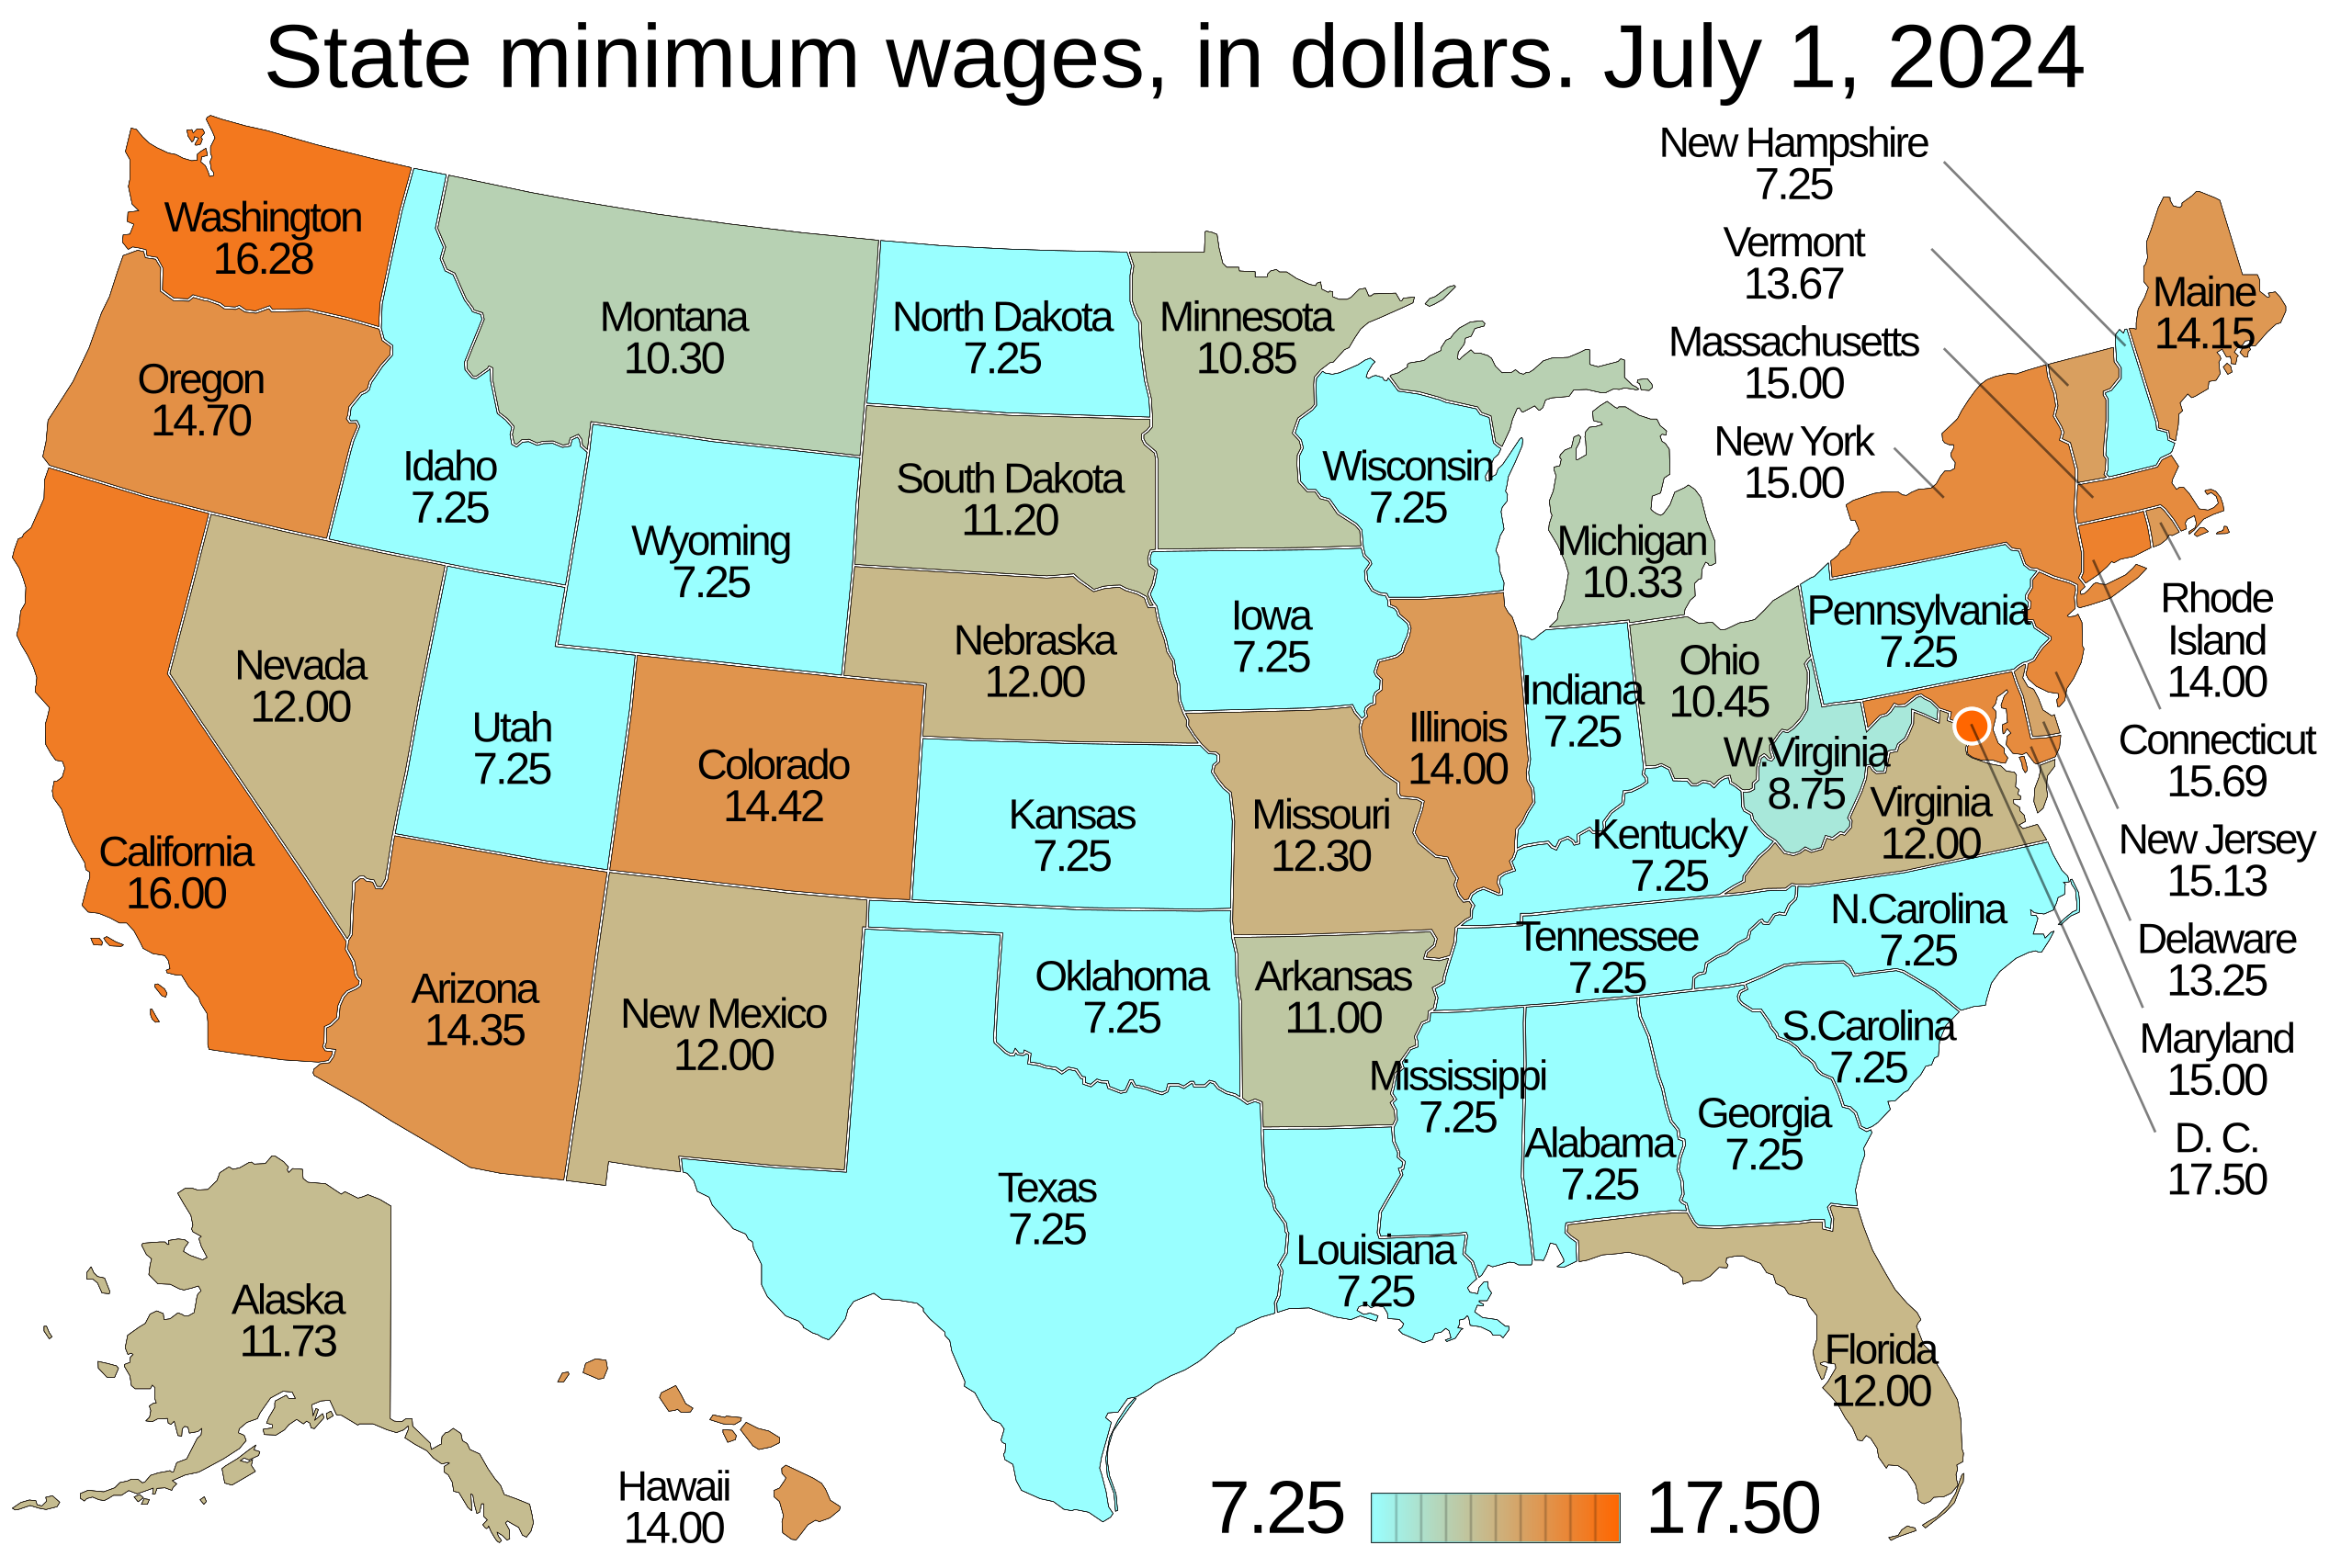
\includegraphics[width=0.7\textwidth,height=\textheight]{figures/minwage.png}

}

\caption{\label{fig-minwage}Minimum wage by state (Source:
\href{https://en.m.wikipedia.org/wiki/File:Map_of_US_minimum_wage_by_state.svg}{Wikipedia})}

\end{figure}%

\end{example}

\section{Differences-in-differences}\label{differences-in-differences}

\subsection{Differences-in-differences with two time
periods}\label{differences-in-differences-with-two-time-periods}

To introduce the differences-in-differences (DiD) approach involving two
groups and two time periods, we introduce the following notation:

\begin{itemize}
\tightlist
\item
  Two groups: treatment group and control group,
\item
  Two time periods: before (\(t=1\)) and after (\(t=2\)) intervention
  (or policy change),
\item
  \(\bar{Y}^{treatment,before}\): the sample average of \(Y\) for the
  treated units before the intervention,
\item
  \(\bar{Y}^{treatment,after}\): the sample average of \(Y\) for the
  treated units after the intervention,
\item
  \(\bar{Y}^{control,before}\): the sample average of \(Y\) for the
  control group before the intervention, and
\item
  \(\bar{Y}^{control,after}\): the sample average of \(Y\) for the
  control group after the intervention.
\end{itemize}

\begin{definition}[The DiD
estimator]\protect\hypertarget{def-def20.5}{}\label{def-def20.5}

The DiD estimator is given by
\begin{equation}\phantomsection\label{eq-eq20.5}{
\begin{align}
\hat{\beta}&=\left(\bar{Y}^{ treatment,after}-\bar{Y}^{treatment,before}\right)-\left(\bar{Y}^{control,after}-\bar{Y}^{control,before}\right)\\
&=\Delta\bar{Y}^{treatment}-\Delta\bar{Y}^{control}.
\end{align}
}\end{equation}

\end{definition}

We illustrate the DiD estimator \(\hat{\beta}\) in
Figure~\ref{fig-f20.2}. Before the treatment, the sample averages are
\(\bar{Y}^{treatment,before}=40\) and \(\bar{Y}^{control,before}=20\),
and after the treatment these averages are
\(\bar{Y}^{treatment,after}=80\) and \(\bar{Y}^{control,after}=30\).
Note that the difference in group means after the treatment is
\(80-30=50\). Some of this difference is due to the fact that both
groups have different pre-treatment means. The DiD approach removes the
effect of the difference in the pre-treatment period by focusing on the
change in group means. Thus, the DiD estimator gives
\((80-40)-(30-20)=30\).

The DiD approach is based on the assumption that, on average, the
treatment and control groups would have followed the same trend in the
absence of treatment. This assumption is called the \textbf{parallel
trends assumption} in the literature. In Figure~\ref{fig-f20.2}, the
trend in the average outcome for the treated group in the absence of
treatment is illustrated with the dashed black line. Thus, the
counterfactual average outcome for the treated group in the
post-treatment period is \(\bar{Y}^{\text{treatment, after}} = 50\), so
that the dashed line is parallel to the steel blue line. This assumption
ensures that the difference between the observed average outcome
\(\bar{Y}^{treatment,after}=80\) and the counterfactual average outcome
\(\bar{Y}^{\text{treatment, after}} = 50\) is due to the treatment.

\begin{Shaded}
\begin{Highlighting}[]
\CommentTok{\# The DiD estimator}
\CommentTok{\# Create a figure and axis object}
\NormalTok{sns.}\BuiltInTok{set}\NormalTok{(style}\OperatorTok{=}\StringTok{\textquotesingle{}darkgrid\textquotesingle{}}\NormalTok{)}
\NormalTok{fig, ax }\OperatorTok{=}\NormalTok{ plt.subplots(figsize}\OperatorTok{=}\NormalTok{(}\DecValTok{7}\NormalTok{, }\DecValTok{5}\NormalTok{))}
\CommentTok{\# Plot scatter points}
\NormalTok{ax.scatter([}\DecValTok{0}\NormalTok{, }\DecValTok{1}\NormalTok{], [}\DecValTok{20}\NormalTok{, }\DecValTok{30}\NormalTok{], color}\OperatorTok{=}\StringTok{\textquotesingle{}steelblue\textquotesingle{}}\NormalTok{, s}\OperatorTok{=}\DecValTok{40}\NormalTok{, label}\OperatorTok{=}\StringTok{\textquotesingle{}Control Group\textquotesingle{}}\NormalTok{)}
\NormalTok{ax.scatter([}\DecValTok{0}\NormalTok{, }\DecValTok{1}\NormalTok{, }\DecValTok{1}\NormalTok{], [}\DecValTok{40}\NormalTok{, }\DecValTok{50}\NormalTok{, }\DecValTok{80}\NormalTok{], color}\OperatorTok{=}\StringTok{\textquotesingle{}black\textquotesingle{}}\NormalTok{, s}\OperatorTok{=}\DecValTok{40}\NormalTok{, label}\OperatorTok{=}\StringTok{\textquotesingle{}Treatment Group\textquotesingle{}}\NormalTok{)}
\CommentTok{\# Plot line segments }
\NormalTok{ax.plot([}\DecValTok{0}\NormalTok{, }\DecValTok{1}\NormalTok{], [}\DecValTok{40}\NormalTok{, }\DecValTok{80}\NormalTok{], color}\OperatorTok{=}\StringTok{\textquotesingle{}black\textquotesingle{}}\NormalTok{, linestyle}\OperatorTok{=}\StringTok{\textquotesingle{}{-}\textquotesingle{}}\NormalTok{, linewidth}\OperatorTok{=}\FloatTok{1.5}\NormalTok{)}
\NormalTok{ax.plot([}\DecValTok{0}\NormalTok{, }\DecValTok{1}\NormalTok{], [}\DecValTok{20}\NormalTok{, }\DecValTok{30}\NormalTok{], color}\OperatorTok{=}\StringTok{\textquotesingle{}steelblue\textquotesingle{}}\NormalTok{, linestyle}\OperatorTok{=}\StringTok{\textquotesingle{}{-}\textquotesingle{}}\NormalTok{, linewidth}\OperatorTok{=}\FloatTok{1.5}\NormalTok{)}
\NormalTok{ax.plot([}\DecValTok{0}\NormalTok{, }\DecValTok{1}\NormalTok{], [}\DecValTok{40}\NormalTok{, }\DecValTok{50}\NormalTok{], color}\OperatorTok{=}\StringTok{\textquotesingle{}black\textquotesingle{}}\NormalTok{, linestyle}\OperatorTok{=}\StringTok{\textquotesingle{}{-}{-}\textquotesingle{}}\NormalTok{, linewidth}\OperatorTok{=}\DecValTok{1}\NormalTok{)}
\NormalTok{ax.plot([}\DecValTok{1}\NormalTok{, }\DecValTok{1}\NormalTok{], [}\DecValTok{50}\NormalTok{, }\DecValTok{80}\NormalTok{], color}\OperatorTok{=}\StringTok{\textquotesingle{}steelblue\textquotesingle{}}\NormalTok{, linestyle}\OperatorTok{=}\StringTok{\textquotesingle{}{-}{-}\textquotesingle{}}\NormalTok{, linewidth}\OperatorTok{=}\DecValTok{1}\NormalTok{)}
\CommentTok{\# Set axis limits and labels}
\NormalTok{ax.set\_ylim(}\DecValTok{0}\NormalTok{, }\DecValTok{90}\NormalTok{) }
\NormalTok{ax.set\_xlim(}\OperatorTok{{-}}\FloatTok{0.5}\NormalTok{, }\FloatTok{1.5}\NormalTok{)}
\NormalTok{ax.set\_xlabel(}\StringTok{\textquotesingle{}Time period\textquotesingle{}}\NormalTok{)}
\NormalTok{ax.set\_ylabel(}\StringTok{\textquotesingle{}Outcome (Y)\textquotesingle{}}\NormalTok{)}
\CommentTok{\# Custom ticks for x and y axes}
\NormalTok{ax.set\_xticks([}\DecValTok{0}\NormalTok{, }\DecValTok{1}\NormalTok{])}
\NormalTok{ax.set\_xticklabels([}\VerbatimStringTok{r\textquotesingle{}$t=1$\textquotesingle{}}\NormalTok{, }\VerbatimStringTok{r\textquotesingle{}$t=2$\textquotesingle{}}\NormalTok{])}
\NormalTok{ax.set\_yticks([}\DecValTok{0}\NormalTok{, }\DecValTok{10}\NormalTok{, }\DecValTok{20}\NormalTok{, }\DecValTok{30}\NormalTok{, }\DecValTok{40}\NormalTok{, }\DecValTok{50}\NormalTok{, }\DecValTok{60}\NormalTok{, }\DecValTok{70}\NormalTok{, }\DecValTok{80}\NormalTok{, }\DecValTok{90}\NormalTok{]) }
\CommentTok{\# Add annotations }
\NormalTok{ax.text(}\FloatTok{1.02}\NormalTok{, }\DecValTok{65}\NormalTok{, }\VerbatimStringTok{r\textquotesingle{}$\textbackslash{}hat\{\textbackslash{}beta\}\^{}}\SpecialCharTok{\{DiD\}}\VerbatimStringTok{$\textquotesingle{}}\NormalTok{, fontsize}\OperatorTok{=}\DecValTok{12}\NormalTok{, ha}\OperatorTok{=}\StringTok{\textquotesingle{}left\textquotesingle{}}\NormalTok{)}
\NormalTok{ax.text(}\DecValTok{0}\NormalTok{, }\DecValTok{13}\NormalTok{, }\VerbatimStringTok{r\textquotesingle{}$\textbackslash{}bar}\SpecialCharTok{\{Y\}}\VerbatimStringTok{\^{}\{\textbackslash{}text\{control,before}\SpecialCharTok{\}\}}\VerbatimStringTok{$\textquotesingle{}}\NormalTok{, fontsize}\OperatorTok{=}\DecValTok{12}\NormalTok{, ha}\OperatorTok{=}\StringTok{\textquotesingle{}left\textquotesingle{}}\NormalTok{)}
\NormalTok{ax.text(}\DecValTok{0}\NormalTok{, }\DecValTok{35}\NormalTok{, }\VerbatimStringTok{r\textquotesingle{}$\textbackslash{}bar}\SpecialCharTok{\{Y\}}\VerbatimStringTok{\^{}\{\textbackslash{}text\{treatment,before}\SpecialCharTok{\}\}}\VerbatimStringTok{$\textquotesingle{}}\NormalTok{, fontsize}\OperatorTok{=}\DecValTok{12}\NormalTok{, ha}\OperatorTok{=}\StringTok{\textquotesingle{}left\textquotesingle{}}\NormalTok{)}
\NormalTok{ax.text(}\DecValTok{1}\NormalTok{, }\DecValTok{33}\NormalTok{, }\VerbatimStringTok{r\textquotesingle{}$\textbackslash{}bar}\SpecialCharTok{\{Y\}}\VerbatimStringTok{\^{}\{\textbackslash{}text\{control,after}\SpecialCharTok{\}\}}\VerbatimStringTok{$\textquotesingle{}}\NormalTok{, fontsize}\OperatorTok{=}\DecValTok{12}\NormalTok{, ha}\OperatorTok{=}\StringTok{\textquotesingle{}left\textquotesingle{}}\NormalTok{)}
\NormalTok{ax.text(}\DecValTok{1}\NormalTok{, }\DecValTok{83}\NormalTok{, }\VerbatimStringTok{r\textquotesingle{}$\textbackslash{}bar}\SpecialCharTok{\{Y\}}\VerbatimStringTok{\^{}\{\textbackslash{}text\{treatment,after}\SpecialCharTok{\}\}}\VerbatimStringTok{$\textquotesingle{}}\NormalTok{, fontsize}\OperatorTok{=}\DecValTok{12}\NormalTok{, ha}\OperatorTok{=}\StringTok{\textquotesingle{}left\textquotesingle{}}\NormalTok{)}
\CommentTok{\# Add legend}
\NormalTok{ax.legend(loc}\OperatorTok{=}\StringTok{"upper left"}\NormalTok{, frameon}\OperatorTok{=}\VariableTok{False}\NormalTok{)}
\NormalTok{plt.show()}
\end{Highlighting}
\end{Shaded}

\begin{figure}[H]

\centering{

\includegraphics{Chapter13-Experiments_files/figure-pdf/fig-f20.2-output-1.pdf}

}

\caption{\label{fig-f20.2}The DiD estimator}

\end{figure}%

The DiD estimator in Equation~\ref{eq-eq20.5} suggests that we can
alternatively compute it using the following regression model:
\begin{equation}\phantomsection\label{eq-eq20.6}{
\begin{align}
\Delta Y_i=\beta_0+\beta_1D_i+u_i,
\end{align}
}\end{equation} where \(\Delta Y_i\) represents the change in the
post-treatment value of \(Y_i\) minus the pre-treatment value for the
\(i\)th individual, and \(D_i\) is the treatment indicator. In this
regression, the DiD estimator is the OLS estimator of
\(\beta_1=\E[\Delta Y_i|D_i=1]-\E[\Delta Y_i|D_i=0]\).

The DiD estimator can be extended to include additional regressors
\(W_{1},\dots,W_{r}\). These variables can be pre-treatment individual
characteristics, or they can be control variables:
\begin{equation}\phantomsection\label{eq-eq20.7}{
\begin{align}
\Delta Y_i=\beta_0+\beta_1D_i+\beta_2W_{1i}+\dots+\beta_{r+1}W_{ri}+u_i.
\end{align}
}\end{equation}

The main reason for including additional regressors
\(W_{1},\dots,W_{r}\) in the DiD model is to ensure that the parallel
trends assumption holds.

\begin{tcolorbox}[enhanced jigsaw, leftrule=.75mm, colbacktitle=quarto-callout-note-color!10!white, coltitle=black, toptitle=1mm, title={Key Concept 20.1: Key features of the DiD approach}, breakable, left=2mm, toprule=.15mm, opacityback=0, titlerule=0mm, opacitybacktitle=0.6, bottomtitle=1mm, colback=white, arc=.35mm, colframe=quarto-callout-note-color-frame, rightrule=.15mm, bottomrule=.15mm]

The key features of the DiD approach are:

\begin{itemize}
\tightlist
\item
  There are two time periods: a pre-treatment period and a
  post-treatment period (or a before and after period).
\item
  There are two groups: a treatment group and a control group. The
  treatment group receives the treatment or is subjected to the policy
  change (intervention) only in the after period. The control group is
  not subjected to the treatment in either periods.
\item
  Parallel trends assumption: In the absence of treatment, the treatment
  group on average would have had the same trend in \(Y\) as the control
  group.
\end{itemize}

\end{tcolorbox}

\subsection{Differences-in-differences with multiple time
periods}\label{differences-in-differences-with-multiple-time-periods}

We assume that there are two periods in the DiD approach so far. It is
also possible to extend the DiD approach when we observe each unit in
the treatment and control group at multiple time periods. Let us assume
that we observe each unit for \(t=1,2,\dots,T\) periods. We also assume
that there is a common treatment timing denoted by \(t_0\). Then, the
DiD estimator can be computed using the following regression:
\begin{equation}\phantomsection\label{eq-eq20.8}{
\begin{align}
Y_{it}=\beta_0+\beta_1D_i+\beta_2{\tt Period}_t+\beta_3(D_i\times{\tt Period}_t)+u_{it},
\end{align}
}\end{equation} where \(D_i\) is the treatment indicator,
\({\tt Period}_t\) is the post-treatment indicator given by \[
\begin{align}
{\tt Period}_t=
\begin{cases}
1\quad\text{if}\quad t\geq t_0,\\
0\quad\text{if}\quad t< t_0.
\end{cases}
\end{align}
\] The DiD estimator is the OLS estimator of \(\beta_3\) in
Equation~\ref{eq-eq20.8}. We can also estimate the DiD parameter
\(\beta_3\) through the following two-way fixed effects regression:
\begin{equation}\phantomsection\label{eq-eq20.9}{
\begin{align}
Y_{it}=\alpha_i+\lambda_t+\beta_3(D_i\times{\tt Period}_t)+u_{it},
\end{align}
}\end{equation} where \(\alpha_i\) is the individual (entity) fixed
effect, \(\lambda_t\) is the time fixed effect, \(D_i\) is the treatment
indicator, and \({\tt Period}_t\) is the post-treatment indicator. The
DiD estimator is given by the fixed effects estimator of \(\beta_3\).
Both Equation~\ref{eq-eq20.8} and Equation~\ref{eq-eq20.9} can also be
extended by considering variables \(W_{1t},\dots,W_{rt}\) on the
pre-treatment individual characteristics.

\subsection{Application: The effect of minimum wage on
employment}\label{application-the-effect-of-minimum-wage-on-employment}

In this section, we replicate some the results from Card and Krueger
(1994). The sample data obtained from Hansen (2022a) is contained in
\texttt{CK1994.xlsx} and consists of two surveys conducted on 331
fast-food restaurants in New Jersey and 79 fast-food restaurants in
eastern Pennsylvania. The first survey was conducted between 2/15/1992
and 3/4/1992 (before the minimum wage increase), and the second between
11/5/1992 and 12/31/1992 (after the wage increase). Some of variables in
the data set are listed below:

\begin{itemize}
\tightlist
\item
  \texttt{store}: Unique store ID
\item
  \texttt{state}: 1 if New Jersey; 0 if Pennsylvania
\item
  \texttt{empft}: Number of full-time employees
\item
  \texttt{emppt}: Number of part-time employees
\item
  \texttt{nmgrs}: Number of managers/assistant managers
\item
  \texttt{wage\_st}: Starting wage (dollars per hour)
\item
  \texttt{inctime}: Months to usual first raise
\item
  \texttt{firstinc}: Usual amount of first raise (dollars/hour)
\item
  \texttt{meals}: Free/reduced price code (see below)
\item
  \texttt{open}: Hour of opening
\item
  \texttt{hoursopen}: Number hours open per day
\item
  \texttt{time}: 0 if first survey (2/15/1992 -- 3/4/1992), 1 if second
  survey (11/5/1992 -- 12/31/1992)
\end{itemize}

\begin{Shaded}
\begin{Highlighting}[]
\NormalTok{df }\OperatorTok{=}\NormalTok{ pd.read\_stata(}\StringTok{"data/CK1994.dta"}\NormalTok{)}
\NormalTok{df.columns}
\end{Highlighting}
\end{Shaded}

\begin{verbatim}
Index(['store', 'chain', 'co_owned', 'state', 'southj', 'centralj', 'northj',
       'pa1', 'pa2', 'shore', 'ncalls', 'empft', 'emppt', 'nmgrs', 'wage_st',
       'inctime', 'firstinc', 'meals', 'open', 'hoursopen', 'pricesoda',
       'pricefry', 'priceentree', 'nregisters', 'nregisters11', 'time'],
      dtype='object')
\end{verbatim}

We start by using Equation~\ref{eq-eq20.5} to estimate the effect of the
change in the minimum hourly wage on employment in New Jersey. In the
following code chunk, we generate sample averages for both groups before
and after the change. These estimates are provided in
Table~\ref{tbl-t20.3}. In New Jersey, the average employment was 20.43
employees per restaurant before the increase in the minimum wage and
20.90 employees per restaurant after the change. In Pennsylvania, these
averages were 23.38 and 21.10, respectively. The DiD estimator in
Equation~\ref{eq-eq20.5} gives \((20.90-20.43)-(21.10-23.38)=2.75\).
Thus, the average employment increases by 2.75 employees per restaurant
after the increase in the minimum wage, a result that contrasts with
conventional economic theory.

\begin{Shaded}
\begin{Highlighting}[]
\CommentTok{\# Compute total employment}
\NormalTok{df[}\StringTok{\textquotesingle{}fte\textquotesingle{}}\NormalTok{] }\OperatorTok{=}\NormalTok{ df[}\StringTok{\textquotesingle{}empft\textquotesingle{}}\NormalTok{] }\OperatorTok{+}\NormalTok{ df[}\StringTok{\textquotesingle{}emppt\textquotesingle{}}\NormalTok{] }\OperatorTok{/} \DecValTok{2} \OperatorTok{+}\NormalTok{ df[}\StringTok{\textquotesingle{}nmgrs\textquotesingle{}}\NormalTok{]}
\CommentTok{\# Drop missing fte values}
\NormalTok{df }\OperatorTok{=}\NormalTok{ df.dropna(subset}\OperatorTok{=}\NormalTok{[}\StringTok{\textquotesingle{}fte\textquotesingle{}}\NormalTok{])}
\CommentTok{\# Group by store and count number of periods per store}
\NormalTok{df[}\StringTok{\textquotesingle{}nperiods\textquotesingle{}}\NormalTok{] }\OperatorTok{=}\NormalTok{ df.groupby(}\StringTok{\textquotesingle{}store\textquotesingle{}}\NormalTok{)[}\StringTok{\textquotesingle{}store\textquotesingle{}}\NormalTok{].transform(}\StringTok{\textquotesingle{}count\textquotesingle{}}\NormalTok{)}
\CommentTok{\# Keep only stores with two periods}
\NormalTok{df }\OperatorTok{=}\NormalTok{ df[df[}\StringTok{\textquotesingle{}nperiods\textquotesingle{}}\NormalTok{] }\OperatorTok{==} \DecValTok{2}\NormalTok{]}
\CommentTok{\# Average Employment at Fast Food Restaurants}
\NormalTok{n1 }\OperatorTok{=}\NormalTok{ np.mean((df[(df[}\StringTok{\textquotesingle{}state\textquotesingle{}}\NormalTok{] }\OperatorTok{==} \DecValTok{1}\NormalTok{) }\OperatorTok{\&}\NormalTok{ (df[}\StringTok{\textquotesingle{}time\textquotesingle{}}\NormalTok{] }\OperatorTok{==} \DecValTok{0}\NormalTok{)][}\StringTok{\textquotesingle{}fte\textquotesingle{}}\NormalTok{]))}
\NormalTok{n2 }\OperatorTok{=}\NormalTok{ np.mean((df[(df[}\StringTok{\textquotesingle{}state\textquotesingle{}}\NormalTok{] }\OperatorTok{==} \DecValTok{1}\NormalTok{) }\OperatorTok{\&}\NormalTok{ (df[}\StringTok{\textquotesingle{}time\textquotesingle{}}\NormalTok{] }\OperatorTok{==} \DecValTok{1}\NormalTok{)][}\StringTok{\textquotesingle{}fte\textquotesingle{}}\NormalTok{]))}
\NormalTok{p1 }\OperatorTok{=}\NormalTok{ np.mean((df[(df[}\StringTok{\textquotesingle{}state\textquotesingle{}}\NormalTok{] }\OperatorTok{==} \DecValTok{0}\NormalTok{) }\OperatorTok{\&}\NormalTok{ (df[}\StringTok{\textquotesingle{}time\textquotesingle{}}\NormalTok{] }\OperatorTok{==} \DecValTok{0}\NormalTok{)][}\StringTok{\textquotesingle{}fte\textquotesingle{}}\NormalTok{]))}
\NormalTok{p2 }\OperatorTok{=}\NormalTok{ np.mean((df[(df[}\StringTok{\textquotesingle{}state\textquotesingle{}}\NormalTok{] }\OperatorTok{==} \DecValTok{0}\NormalTok{) }\OperatorTok{\&}\NormalTok{ (df[}\StringTok{\textquotesingle{}time\textquotesingle{}}\NormalTok{] }\OperatorTok{==} \DecValTok{1}\NormalTok{)][}\StringTok{\textquotesingle{}fte\textquotesingle{}}\NormalTok{]))}
\CommentTok{\# Collect means in a dataframe}
\NormalTok{c1 }\OperatorTok{=}\NormalTok{ [n1,n2,n2}\OperatorTok{{-}}\NormalTok{n1]}
\NormalTok{c2 }\OperatorTok{=}\NormalTok{ [p1,p2,p2}\OperatorTok{{-}}\NormalTok{p1]}
\NormalTok{d1 }\OperatorTok{=}\NormalTok{ [p1}\OperatorTok{{-}}\NormalTok{n1,p2}\OperatorTok{{-}}\NormalTok{n2,(n2}\OperatorTok{{-}}\NormalTok{n1)}\OperatorTok{{-}}\NormalTok{(p2}\OperatorTok{{-}}\NormalTok{p1)]}
\NormalTok{tb }\OperatorTok{=}\NormalTok{ pd.DataFrame(\{}\StringTok{"New Jersey"}\NormalTok{: c1, }\StringTok{"Pennsylvania"}\NormalTok{: c2,}\StringTok{"Difference"}\NormalTok{:d1\})}
\NormalTok{tb.index}\OperatorTok{=}\NormalTok{[}\StringTok{"Before Increase"}\NormalTok{,}\StringTok{"After Increase"}\NormalTok{,}\StringTok{"Difference"}\NormalTok{]}
\NormalTok{tb.astype(}\BuiltInTok{float}\NormalTok{).}\BuiltInTok{round}\NormalTok{(}\DecValTok{2}\NormalTok{)}
\end{Highlighting}
\end{Shaded}

\begin{figure}

\begin{minipage}{\linewidth}

\begin{longtable}[]{@{}llll@{}}

\caption{\label{tbl-t20.3}Average Employment at Fast Food Restaurants}

\tabularnewline

\toprule\noalign{}
& New Jersey & Pennsylvania & Difference \\
\midrule\noalign{}
\endhead
\bottomrule\noalign{}
\endlastfoot
Before Increase & 20.43 & 23.38 & 2.95 \\
After Increase & 20.90 & 21.10 & 0.20 \\
Difference & 0.47 & -2.28 & 2.75 \\

\end{longtable}

\end{minipage}%

\end{figure}%

Next, we use Equation~\ref{eq-eq20.6} to estimate the effect of the
increase in the minimum wage on employment. In the following code chunk,
we generate the \(\Delta Y\) and \(D\) variables, and then use the OLS
estimator to estimate the DiD parameter \(\beta_1\). The DiD estimate of
\(\beta_1\) is \(2.75\), which is exactly the same as the one in
Table~\ref{tbl-t20.3}.

\begin{Shaded}
\begin{Highlighting}[]
\NormalTok{DeltaY}\OperatorTok{=}\NormalTok{df.fte[df.time}\OperatorTok{==}\DecValTok{1}\NormalTok{].values}\OperatorTok{{-}}\NormalTok{df.fte[df.time}\OperatorTok{==}\DecValTok{0}\NormalTok{].values}
\NormalTok{D}\OperatorTok{=}\NormalTok{df.state[df.time}\OperatorTok{==}\DecValTok{1}\NormalTok{]}
\NormalTok{df1}\OperatorTok{=}\NormalTok{pd.DataFrame(\{}\StringTok{"DeltaY"}\NormalTok{:DeltaY,}\StringTok{"D"}\NormalTok{:D\})}
\NormalTok{model1 }\OperatorTok{=}\NormalTok{ smf.ols(}\StringTok{\textquotesingle{}DeltaY \textasciitilde{} D\textquotesingle{}}\NormalTok{, data}\OperatorTok{=}\NormalTok{df1)}
\NormalTok{result1}\OperatorTok{=}\NormalTok{model1.fit(cov\_type}\OperatorTok{=}\StringTok{\textquotesingle{}HC1\textquotesingle{}}\NormalTok{)}
\BuiltInTok{print}\NormalTok{(result1.summary())}
\end{Highlighting}
\end{Shaded}

\begin{verbatim}
                            OLS Regression Results                            
==============================================================================
Dep. Variable:                 DeltaY   R-squared:                       0.015
Model:                            OLS   Adj. R-squared:                  0.012
Method:                 Least Squares   F-statistic:                     4.226
Date:                Sun, 10 Aug 2025   Prob (F-statistic):             0.0405
Time:                        14:40:12   Log-Likelihood:                -1386.2
No. Observations:                 384   AIC:                             2776.
Df Residuals:                     382   BIC:                             2784.
Df Model:                           1                                         
Covariance Type:                  HC1                                         
==============================================================================
                 coef    std err          z      P>|z|      [0.025      0.975]
------------------------------------------------------------------------------
Intercept     -2.2833      1.248     -1.829      0.067      -4.730       0.163
D              2.7500      1.338      2.056      0.040       0.128       5.372
==============================================================================
Omnibus:                       33.136   Durbin-Watson:                   2.201
Prob(Omnibus):                  0.000   Jarque-Bera (JB):               94.711
Skew:                          -0.361   Prob(JB):                     2.71e-21
Kurtosis:                       5.323   Cond. No.                         4.32
==============================================================================

Notes:
[1] Standard Errors are heteroscedasticity robust (HC1)
\end{verbatim}

We can also use Equation~\ref{eq-eq20.8} to estimate the DiD parameter
\(\beta_3\). In the following code chunk, we first create the
\texttt{treatment} variable, which represents
\(D_i \times {\tt Period}_t\), and then use the OLS estimator to
estimate \(\beta_3\). Note that we use clustered standard errors at the
store level to account for correlation in the error terms across stores.
The DiD estimate of \(\beta_3\) is 2.75 with a \(t\)-value of 2.05.

\begin{Shaded}
\begin{Highlighting}[]
\CommentTok{\# Estimation of (20.7)}
\CommentTok{\# Create treatment variable}
\NormalTok{df[}\StringTok{\textquotesingle{}treatment\textquotesingle{}}\NormalTok{] }\OperatorTok{=}\NormalTok{ df[}\StringTok{\textquotesingle{}time\textquotesingle{}}\NormalTok{] }\OperatorTok{*}\NormalTok{ df[}\StringTok{\textquotesingle{}state\textquotesingle{}}\NormalTok{]}

\CommentTok{\# Simple OLS regression with clustering on store}
\NormalTok{model2 }\OperatorTok{=}\NormalTok{ smf.ols(}\StringTok{\textquotesingle{}fte \textasciitilde{} state + time + treatment\textquotesingle{}}\NormalTok{, data}\OperatorTok{=}\NormalTok{df)}
\NormalTok{result2 }\OperatorTok{=}\NormalTok{ model2.fit(cov\_type}\OperatorTok{=}\StringTok{\textquotesingle{}cluster\textquotesingle{}}\NormalTok{, cov\_kwds}\OperatorTok{=}\NormalTok{\{}\StringTok{\textquotesingle{}groups\textquotesingle{}}\NormalTok{: df[}\StringTok{\textquotesingle{}store\textquotesingle{}}\NormalTok{]\})}
\BuiltInTok{print}\NormalTok{(result2.summary())}
\end{Highlighting}
\end{Shaded}

\begin{verbatim}
                            OLS Regression Results                            
==============================================================================
Dep. Variable:                    fte   R-squared:                       0.008
Model:                            OLS   Adj. R-squared:                  0.004
Method:                 Least Squares   F-statistic:                     1.655
Date:                Sun, 10 Aug 2025   Prob (F-statistic):              0.176
Time:                        14:40:12   Log-Likelihood:                -2817.6
No. Observations:                 768   AIC:                             5643.
Df Residuals:                     764   BIC:                             5662.
Df Model:                           3                                         
Covariance Type:              cluster                                         
==============================================================================
                 coef    std err          z      P>|z|      [0.025      0.975]
------------------------------------------------------------------------------
Intercept     23.3800      1.382     16.917      0.000      20.671      26.089
state         -2.9494      1.478     -1.995      0.046      -5.847      -0.052
time          -2.2833      1.249     -1.828      0.068      -4.731       0.165
treatment      2.7500      1.339      2.054      0.040       0.126       5.374
==============================================================================
Omnibus:                      212.243   Durbin-Watson:                   1.835
Prob(Omnibus):                  0.000   Jarque-Bera (JB):              761.734
Skew:                           1.278   Prob(JB):                    3.90e-166
Kurtosis:                       7.155   Cond. No.                         11.3
==============================================================================

Notes:
[1] Standard Errors are robust to cluster correlation (cluster)
\end{verbatim}

Finally, we use the two-way fixed effects model in
Equation~\ref{eq-eq20.9} to estimate the DiD parameter \(\beta_3\). The
following code chunk provides the same estimate as the previous methods.

\begin{Shaded}
\begin{Highlighting}[]
\CommentTok{\# Setting panel structure}
\NormalTok{df[}\StringTok{"Time"}\NormalTok{] }\OperatorTok{=}\NormalTok{ df.time}
\NormalTok{df\_panel }\OperatorTok{=}\NormalTok{ df.set\_index([}\StringTok{\textquotesingle{}store\textquotesingle{}}\NormalTok{, }\StringTok{\textquotesingle{}time\textquotesingle{}}\NormalTok{])}

\CommentTok{\# Fixed effects panel regression}
\NormalTok{model3 }\OperatorTok{=}\NormalTok{ PanelOLS.from\_formula(}\StringTok{\textquotesingle{}fte \textasciitilde{} treatment + EntityEffects + Time\textquotesingle{}}\NormalTok{, df\_panel)}
\NormalTok{result3 }\OperatorTok{=}\NormalTok{ model3.fit(cov\_type}\OperatorTok{=}\StringTok{\textquotesingle{}clustered\textquotesingle{}}\NormalTok{, cluster\_entity}\OperatorTok{=}\VariableTok{True}\NormalTok{)}
\BuiltInTok{print}\NormalTok{(result3.summary)}
\end{Highlighting}
\end{Shaded}

\begin{verbatim}
                          PanelOLS Estimation Summary                           
================================================================================
Dep. Variable:                    fte   R-squared:                        0.0147
Estimator:                   PanelOLS   R-squared (Between):             -0.0048
No. Observations:                 768   R-squared (Within):               0.0147
Date:                Sun, Aug 10 2025   R-squared (Overall):             -0.0041
Time:                        14:40:12   Log-likelihood                   -2240.1
Cov. Estimator:             Clustered                                           
                                        F-statistic:                      2.8495
Entities:                         384   P-value                           0.0591
Avg Obs:                       2.0000   Distribution:                   F(2,382)
Min Obs:                       2.0000                                           
Max Obs:                       2.0000   F-statistic (robust):             2.1490
                                        P-value                           0.1180
Time periods:                       2   Distribution:                   F(2,382)
Avg Obs:                       384.00                                           
Min Obs:                       384.00                                           
Max Obs:                       384.00                                           
                                                                                
                             Parameter Estimates                              
==============================================================================
            Parameter  Std. Err.     T-stat    P-value    Lower CI    Upper CI
------------------------------------------------------------------------------
Time          -2.2833     1.2465    -1.8318     0.0678     -4.7342      0.1675
treatment      2.7500     1.3360     2.0584     0.0402      0.1232      5.3768
==============================================================================

F-test for Poolability: 3.5246
P-value: 0.0000
Distribution: F(383,382)

Included effects: Entity
\end{verbatim}

\subsection{Identification of the differences-in-differences
parameter}\label{identification-of-the-differences-in-differences-parameter}

n this section, we use the potential outcomes framework to define the
DiD parameter and then state assumptions under which the DiD parameter
is identified. We assume a setting with multiple time periods and a
common treatment timing denoted by \(t_0\), which is the time period
when the treatment starts. Let \(Y_{it}(0)\) and \(Y_{it}(1)\) denote
the untreated and treated potential outcomes for unit \(i\) at period
\(t\). For example, \(Y_{it_0}(1)\) represents the treated potential
outcome for unit \(i\) in period \(t_0\), while \(Y_{i,t_0-1}(0)\)
represents the untreated potential outcome for unit \(i\) in period
\(t_0-1\). Also, recall that \(D_i\) denotes the treatment indicator,
which takes the value 1 for the treated units and 0 for the units in the
control group. The target parameter of interest in this DiD design is
usually the \textbf{average treatment effect on the treated} at time
\(t\), which is defined as \[
\text{ATT}(t)=\E[Y_{it}(1)-Y_{it}(0)|D_i=1].
\]

The \(\text{ATT}(t)\) represents the average difference between treated
and untreated potential outcomes for the treatment group in period
\(t\). To show that \(\text{ATT}(t)\) is identified, we need the
following assumptions.

\begin{tcolorbox}[enhanced jigsaw, leftrule=.75mm, colbacktitle=quarto-callout-important-color!10!white, coltitle=black, toptitle=1mm, title={Assumptions for ATT}, breakable, left=2mm, toprule=.15mm, opacityback=0, titlerule=0mm, opacitybacktitle=0.6, bottomtitle=1mm, colback=white, arc=.35mm, colframe=quarto-callout-important-color-frame, rightrule=.15mm, bottomrule=.15mm]

\begin{enumerate}
\def\labelenumi{\arabic{enumi}.}
\tightlist
\item
  Parallel trends assumption: The potential outcomes satisfy \[
  \E\left[Y_{it}(0)-Y_{i,t_0-1}(0)|D_i=1\right]=\E\left[Y_{it}(0)-Y_{i,t_0-1}(0)|D_i=0\right] 
  \] for \(t\ge t_0\).
\item
  No anticipation assumption: The potential outcomes satisfy \[
  \E\left[Y_{it}(0)|D_i=1\right]=\E\left[Y_{it}(1)|D_i=1\right] 
  \] for \(t<t_0\).
\end{enumerate}

\end{tcolorbox}

The parallel trends assumption requires the average change in the
untreated potential outcomes to be the same for both treatment and
control groups. The no anticipation assumption states that the untreated
and treated potential outcomes of the treated units in the pre-treatment
periods are on average equal. That is, receiving treatment in the
post-treatment periods does not affect the average potential outcomes in
the the pre-treatment periods on average. Hence, \(\text{ATT}(t)=0\) for
\(t<t_0\).

\begin{theorem}[Identification of the ATT
parameter]\protect\hypertarget{thm-th20.2}{}\label{thm-th20.2}

Under the parallel trends and no anticipation assumptions, the average
treatment effect on the treated at time \(t\ge t_0\) is identified as
\[\text{ATT}(t)=\E[\Delta Y_{it}|D_i=1]-\E[\Delta Y_{it}|D_i=0],\] where
\(\Delta Y_{it}=Y_{it}-Y_{i,t_0-1}\) is the change in the observed
outcome for unit \(i\) from period \(t_0-1\) to period \(t\).

\end{theorem}

\begin{proof}[Proof of Theorem~\ref{thm-th20.2}]
Under the two assumptions above, for \(t\ge t_0\), we have \[
\begin{align}
\text{ATT}(t)&=\E[Y_{it}(1)-Y_{it}(0)|D_i=1]\\
&=\E[Y_{it}(1)-Y_{i,t_0-1}(0)|D_i=1]-\E[Y_{it}(0)-Y_{i,t_0-1}(0)|D_i=1]\\
&=\E[Y_{it}(1)-Y_{i,t_0-1}(0)|D_i=1]-\E[Y_{it}(0)-Y_{i,t_0-1}(0)|D_i=0]\\
&=\E[Y_{it}-Y_{i,t_0-1}|D_i=1]-\E[Y_{it}-Y_{i,t_0-1}|D_i=0]\\
&=\E[\Delta Y_{it}|D_i=1]-\E[\Delta Y_{it}|D_i=0],
\end{align}
\] where the second equality follows by adding and substracting
\(\E[Y_{i,t_0-1}(0)|D_i=1]\), the third equality from the parallel
trends assumption, and the fourth equality holds because \(Y_{it}(1)\)
and \(Y_{i,t_0-1}(0)\) are equal to the observed outcomes for the
treatment group under no anticipation, while \(Y_{it}(0)\) and
\(Y_{i,t_0-1}(0)\) are equal to the observed outcomes for the control
group.
\end{proof}

The identification result suggests that the ATT(\(t\)) for \(t\ge t_0\)
can be estimated by the DiD estimator in the 2-period case. To this end,
the DiD estimator in Equation~\ref{eq-eq20.5} (or
Equation~\ref{eq-eq20.6} or Equation~\ref{eq-eq20.7}) can be used by
considering \(t_0-1\) as the first period and \(t\) as the second
period.

In the multiple time period case, we can consider the following two-way
fixed effects specification for estimating the ATT parameters:
\begin{equation}\phantomsection\label{eq-eq20.10}{
Y_{it} = \alpha_i + \lambda_t + \sum_{s=1}^{t_0-2}\beta_s (D_i\times P_s) + \sum_{s=t_0}^{T}\beta_s (D_i\times P_s) + u_{it}
}\end{equation} where \(P_s=1\) if \(s=t\) and \(P_s=0\) otherwise. The
estimates of \(\beta_s\) for \(s\ge t_0\) correspond to the estimates of
\(\text{ATT}(t)\) for \(t\ge t_0\).

This approach allows us using \(t\)-statistics and confidence intervals
based on clustered standard errors. We can then plot ATT estimates along
(point-wise) confidence intervals to summarize our results. This is
often referred to as an \textbf{event study analysis}. Note also that
\(\beta_s\) estimates for the pre-treatment periods can be utilized to
assess the plausibility of the parallel trends assumption. If the
parallel trends assumption holds, then the estimates of \(\beta_s\) for
\(s<t_0\) should be statistically insignificant.

\subsection{Application: Impact of policing on
crime}\label{application-impact-of-policing-on-crime}

We revisit Tella and Schargrodsky (2004) to study the causal effect of
police presence on crime. The dataset is contained in the
\texttt{DS2004.dta} file, which was obtained from Hansen (2022a). The
intervention studied in Tella and Schargrodsky (2004) involves the
assignment of more police protection to certain blocks in Buenos Aires
following the terrorist attack on main Jewish center in July 1994. The
data consist of monthly observations on 876 blocks of which 37 blocks
are provided with extra police protection and cover the time period from
April to December of 1994, excluding July. Therefore, April to June
constitute the pre-treatment months, while August to December represent
the post-treatment period.

Some of the variables included in the dataset are listed below:

\begin{itemize}
\tightlist
\item
  \texttt{thefts}: average number of motor vehicle thefts
\item
  \texttt{treat}: treatment indicator that equals 1 if the block is
  treated, otherwise 0
\item
  \texttt{post}: post treatment indicator that equals to 1 if the
  observation is from the post-treatment period
\item
  \texttt{month}: month
\item
  \texttt{block}: block id
\end{itemize}

The outcome variable is \texttt{thefts} which is the average monthly
number of motor vehicle thefts. Below, we load the data and create the
\texttt{treat} and \texttt{post} variables. The \texttt{treat} variable
is the treatment indicator and the \texttt{post} variable is the
post-treatment indicator. We present the summary statistics of the data
in Table~\ref{tbl-t20.4}. According to this table, 4.2\% of the blocks
are treated, and the average number of car theft is around 0.093.

\begin{Shaded}
\begin{Highlighting}[]
\CommentTok{\# Load the data}
\NormalTok{df }\OperatorTok{=}\NormalTok{ pd.read\_stata(}\StringTok{"data/DS2004.dta"}\NormalTok{)}
\NormalTok{df.rename(columns}\OperatorTok{=}\NormalTok{\{}\StringTok{\textquotesingle{}sameblock\textquotesingle{}}\NormalTok{: }\StringTok{\textquotesingle{}treat\textquotesingle{}}\NormalTok{\}, inplace}\OperatorTok{=}\VariableTok{True}\NormalTok{)}
\NormalTok{df[}\StringTok{\textquotesingle{}post\textquotesingle{}}\NormalTok{] }\OperatorTok{=}\NormalTok{ (df[}\StringTok{\textquotesingle{}month\textquotesingle{}}\NormalTok{] }\OperatorTok{\textgreater{}} \DecValTok{7}\NormalTok{).astype(}\BuiltInTok{int}\NormalTok{)}
\end{Highlighting}
\end{Shaded}

\begin{Shaded}
\begin{Highlighting}[]
\CommentTok{\# Summary statistics}
\NormalTok{df.describe().}\BuiltInTok{round}\NormalTok{(}\DecValTok{3}\NormalTok{).T}
\end{Highlighting}
\end{Shaded}

\begin{figure}

\begin{minipage}{\linewidth}

\begin{longtable}[]{@{}lllllllll@{}}

\caption{\label{tbl-t20.4}Summary statistics}

\tabularnewline

\toprule\noalign{}
& count & mean & std & min & 25\% & 50\% & 75\% & max \\
\midrule\noalign{}
\endhead
\bottomrule\noalign{}
\endlastfoot
block & 7884.0 & 438.500 & 252.897 & 1.0 & 219.75 & 438.5 & 657.25 &
876.0 \\
treat & 7884.0 & 0.042 & 0.201 & 0.0 & 0.00 & 0.0 & 0.00 & 1.0 \\
distance & 7884.0 & 3.014 & 2.007 & 0.0 & 2.00 & 3.0 & 4.00 & 11.0 \\
public & 7884.0 & 0.032 & 0.176 & 0.0 & 0.00 & 0.0 & 0.00 & 1.0 \\
gasstation & 7884.0 & 0.021 & 0.142 & 0.0 & 0.00 & 0.0 & 0.00 & 1.0 \\
bank & 7884.0 & 0.079 & 0.269 & 0.0 & 0.00 & 0.0 & 0.00 & 1.0 \\
thefts & 7884.0 & 0.093 & 0.242 & 0.0 & 0.00 & 0.0 & 0.00 & 2.5 \\
month & 7884.0 & 8.000 & 2.582 & 4.0 & 6.00 & 8.0 & 10.00 & 12.0 \\
oneblock & 7884.0 & 0.184 & 0.387 & 0.0 & 0.00 & 0.0 & 0.00 & 1.0 \\
post & 7884.0 & 0.556 & 0.497 & 0.0 & 0.00 & 1.0 & 1.00 & 1.0 \\

\end{longtable}

\end{minipage}%

\end{figure}%

We first consider estimating the average treatment effect in the
post-period. To this end, we use Equation~\ref{eq-eq20.9} as if we have
only 2 periods, pre- and post-treament. We can use the
\texttt{PanelOLS()} function from \texttt{linearmodels} module to
estimate the model. We use the clustered standard errors at the block
level to account for correlation in the error terms within blocks.

\begin{Shaded}
\begin{Highlighting}[]
\CommentTok{\# Convert the data to a panel data structure}
\NormalTok{df\_panel }\OperatorTok{=}\NormalTok{ df.set\_index([}\StringTok{\textquotesingle{}block\textquotesingle{}}\NormalTok{, }\StringTok{\textquotesingle{}month\textquotesingle{}}\NormalTok{])}

\CommentTok{\# Estimate the model using PanelOLS}
\NormalTok{model4 }\OperatorTok{=}\NormalTok{ PanelOLS.from\_formula(}\StringTok{\textquotesingle{}thefts \textasciitilde{} I(treat*post) + EntityEffects + TimeEffects\textquotesingle{}}\NormalTok{, df\_panel)}
\NormalTok{result4 }\OperatorTok{=}\NormalTok{ model4.fit(cov\_type}\OperatorTok{=}\StringTok{\textquotesingle{}clustered\textquotesingle{}}\NormalTok{, cluster\_entity}\OperatorTok{=}\VariableTok{True}\NormalTok{)}
\BuiltInTok{print}\NormalTok{(result4.summary)}
\end{Highlighting}
\end{Shaded}

\begin{verbatim}
                          PanelOLS Estimation Summary                           
================================================================================
Dep. Variable:                 thefts   R-squared:                        0.0013
Estimator:                   PanelOLS   R-squared (Between):             -0.0149
No. Observations:                7884   R-squared (Within):               0.0005
Date:                Sun, Aug 10 2025   R-squared (Overall):             -0.0040
Time:                        14:40:12   Log-likelihood                    870.52
Cov. Estimator:             Clustered                                           
                                        F-statistic:                      8.9506
Entities:                         876   P-value                           0.0028
Avg Obs:                       9.0000   Distribution:                  F(1,6999)
Min Obs:                       9.0000                                           
Max Obs:                       9.0000   F-statistic (robust):             9.6788
                                        P-value                           0.0019
Time periods:                       9   Distribution:                  F(1,6999)
Avg Obs:                       876.00                                           
Min Obs:                       876.00                                           
Max Obs:                       876.00                                           
                                                                                
                               Parameter Estimates                               
=================================================================================
               Parameter  Std. Err.     T-stat    P-value    Lower CI    Upper CI
---------------------------------------------------------------------------------
I(treat*post)    -0.0775     0.0249    -3.1111     0.0019     -0.1264     -0.0287
=================================================================================

F-test for Poolability: 1.9474
P-value: 0.0000
Distribution: F(883,6999)

Included effects: Entity, Time
\end{verbatim}

The estimate of the average treatment effect (on treated blocks) in the
post-period is \(-0.078\), i.e., police presence, on average, reduced
car thefts by \(0.078\) in the treated blocks. This estimate is almost
the same as the one reported in the first column of Table 3 in Tella and
Schargrodsky (2004). Given that the average number of car theft is
around \(0.093\), this estimate is not negligible.

Next, we will consider an event study analysis and estimate
Equation~\ref{eq-eq20.10}. First, we need to generate the interactions
of the treatment dummy with pre and post periods.

\begin{Shaded}
\begin{Highlighting}[]
\NormalTok{df[}\StringTok{\textquotesingle{}lead4\textquotesingle{}}\NormalTok{] }\OperatorTok{=}\NormalTok{ ((df[}\StringTok{\textquotesingle{}treat\textquotesingle{}}\NormalTok{] }\OperatorTok{==} \DecValTok{1}\NormalTok{) }\OperatorTok{\&}\NormalTok{ (df[}\StringTok{\textquotesingle{}month\textquotesingle{}}\NormalTok{] }\OperatorTok{==} \DecValTok{4}\NormalTok{)).astype(}\BuiltInTok{int}\NormalTok{) }\CommentTok{\# april}
\NormalTok{df[}\StringTok{\textquotesingle{}lead3\textquotesingle{}}\NormalTok{] }\OperatorTok{=}\NormalTok{ ((df[}\StringTok{\textquotesingle{}treat\textquotesingle{}}\NormalTok{] }\OperatorTok{==} \DecValTok{1}\NormalTok{) }\OperatorTok{\&}\NormalTok{ (df[}\StringTok{\textquotesingle{}month\textquotesingle{}}\NormalTok{] }\OperatorTok{==} \DecValTok{5}\NormalTok{)).astype(}\BuiltInTok{int}\NormalTok{) }\CommentTok{\# may}
\NormalTok{df[}\StringTok{\textquotesingle{}lead2\textquotesingle{}}\NormalTok{] }\OperatorTok{=}\NormalTok{ ((df[}\StringTok{\textquotesingle{}treat\textquotesingle{}}\NormalTok{] }\OperatorTok{==} \DecValTok{1}\NormalTok{) }\OperatorTok{\&}\NormalTok{ (df[}\StringTok{\textquotesingle{}month\textquotesingle{}}\NormalTok{] }\OperatorTok{==} \DecValTok{6}\NormalTok{)).astype(}\BuiltInTok{int}\NormalTok{) }\CommentTok{\# june}
\NormalTok{df[}\StringTok{\textquotesingle{}lead1\textquotesingle{}}\NormalTok{] }\OperatorTok{=}\NormalTok{ ((df[}\StringTok{\textquotesingle{}treat\textquotesingle{}}\NormalTok{] }\OperatorTok{==} \DecValTok{1}\NormalTok{) }\OperatorTok{\&}\NormalTok{ (df[}\StringTok{\textquotesingle{}month\textquotesingle{}}\NormalTok{] }\OperatorTok{==} \DecValTok{7}\NormalTok{)).astype(}\BuiltInTok{int}\NormalTok{) }\CommentTok{\# july}
\NormalTok{df[}\StringTok{\textquotesingle{}lead0\textquotesingle{}}\NormalTok{] }\OperatorTok{=}\NormalTok{ ((df[}\StringTok{\textquotesingle{}treat\textquotesingle{}}\NormalTok{] }\OperatorTok{==} \DecValTok{1}\NormalTok{) }\OperatorTok{\&}\NormalTok{ (df[}\StringTok{\textquotesingle{}month\textquotesingle{}}\NormalTok{] }\OperatorTok{==} \DecValTok{8}\NormalTok{)).astype(}\BuiltInTok{int}\NormalTok{) }\CommentTok{\# august}
\NormalTok{df[}\StringTok{\textquotesingle{}lag1\textquotesingle{}}\NormalTok{] }\OperatorTok{=}\NormalTok{ ((df[}\StringTok{\textquotesingle{}treat\textquotesingle{}}\NormalTok{] }\OperatorTok{==} \DecValTok{1}\NormalTok{) }\OperatorTok{\&}\NormalTok{ (df[}\StringTok{\textquotesingle{}month\textquotesingle{}}\NormalTok{] }\OperatorTok{==} \DecValTok{9}\NormalTok{)).astype(}\BuiltInTok{int}\NormalTok{)  }\CommentTok{\# september}
\NormalTok{df[}\StringTok{\textquotesingle{}lag2\textquotesingle{}}\NormalTok{] }\OperatorTok{=}\NormalTok{ ((df[}\StringTok{\textquotesingle{}treat\textquotesingle{}}\NormalTok{] }\OperatorTok{==} \DecValTok{1}\NormalTok{) }\OperatorTok{\&}\NormalTok{ (df[}\StringTok{\textquotesingle{}month\textquotesingle{}}\NormalTok{] }\OperatorTok{==} \DecValTok{10}\NormalTok{)).astype(}\BuiltInTok{int}\NormalTok{) }\CommentTok{\# october}
\NormalTok{df[}\StringTok{\textquotesingle{}lag3\textquotesingle{}}\NormalTok{] }\OperatorTok{=}\NormalTok{ ((df[}\StringTok{\textquotesingle{}treat\textquotesingle{}}\NormalTok{] }\OperatorTok{==} \DecValTok{1}\NormalTok{) }\OperatorTok{\&}\NormalTok{ (df[}\StringTok{\textquotesingle{}month\textquotesingle{}}\NormalTok{] }\OperatorTok{==} \DecValTok{11}\NormalTok{)).astype(}\BuiltInTok{int}\NormalTok{) }\CommentTok{\# november}
\NormalTok{df[}\StringTok{\textquotesingle{}lag4\textquotesingle{}}\NormalTok{] }\OperatorTok{=}\NormalTok{ ((df[}\StringTok{\textquotesingle{}treat\textquotesingle{}}\NormalTok{] }\OperatorTok{==} \DecValTok{1}\NormalTok{) }\OperatorTok{\&}\NormalTok{ (df[}\StringTok{\textquotesingle{}month\textquotesingle{}}\NormalTok{] }\OperatorTok{==} \DecValTok{12}\NormalTok{)).astype(}\BuiltInTok{int}\NormalTok{) }\CommentTok{\# december}
\end{Highlighting}
\end{Shaded}

The common treatment timing \(t_0\) is August and the \(t_0-1\) period
is July. Thus, in the event study analysis, July will be the baseline
period (reference period) and \(\beta_{\text{july}}=0\). We use the
fixed effects estimator to estimate the event study regression in
Equation~\ref{eq-eq20.10}.

\begin{Shaded}
\begin{Highlighting}[]
\CommentTok{\# Convert the data to a panel data structure}
\NormalTok{df\_panel }\OperatorTok{=}\NormalTok{ df.set\_index([}\StringTok{\textquotesingle{}block\textquotesingle{}}\NormalTok{, }\StringTok{\textquotesingle{}month\textquotesingle{}}\NormalTok{])}

\CommentTok{\# Estimate the model using PanelOLS}
\NormalTok{formula }\OperatorTok{=} \StringTok{\textquotesingle{}thefts \textasciitilde{} lead4 + lead3 + lead2 + lead0 + lag1 + lag2 + lag3 + lag4 + EntityEffects + TimeEffects\textquotesingle{}}
\NormalTok{model5 }\OperatorTok{=}\NormalTok{ PanelOLS.from\_formula(formula, df\_panel)}
\NormalTok{result5 }\OperatorTok{=}\NormalTok{ model5.fit(cov\_type}\OperatorTok{=}\StringTok{\textquotesingle{}clustered\textquotesingle{}}\NormalTok{, cluster\_entity}\OperatorTok{=}\VariableTok{True}\NormalTok{)}
\BuiltInTok{print}\NormalTok{(result5.summary)}
\end{Highlighting}
\end{Shaded}

\begin{verbatim}
                          PanelOLS Estimation Summary                           
================================================================================
Dep. Variable:                 thefts   R-squared:                        0.0017
Estimator:                   PanelOLS   R-squared (Between):             -0.0041
No. Observations:                7884   R-squared (Within):               0.0011
Date:                Sun, Aug 10 2025   R-squared (Overall):             -0.0004
Time:                        14:40:12   Log-likelihood                    872.05
Cov. Estimator:             Clustered                                           
                                        F-statistic:                      1.4589
Entities:                         876   P-value                           0.1667
Avg Obs:                       9.0000   Distribution:                  F(8,6992)
Min Obs:                       9.0000                                           
Max Obs:                       9.0000   F-statistic (robust):             2.8981
                                        P-value                           0.0032
Time periods:                       9   Distribution:                  F(8,6992)
Avg Obs:                       876.00                                           
Min Obs:                       876.00                                           
Max Obs:                       876.00                                           
                                                                                
                             Parameter Estimates                              
==============================================================================
            Parameter  Std. Err.     T-stat    P-value    Lower CI    Upper CI
------------------------------------------------------------------------------
lag1          -0.0646     0.0193    -3.3491     0.0008     -0.1024     -0.0268
lag2          -0.0265     0.0413    -0.6417     0.5211     -0.1075      0.0545
lag3          -0.0528     0.0217    -2.4375     0.0148     -0.0953     -0.0103
lag4          -0.0582     0.0218    -2.6642     0.0077     -0.1010     -0.0154
lead0         -0.0430     0.0353    -1.2168     0.2237     -0.1123      0.0263
lead2          0.0729     0.0479     1.5214     0.1282     -0.0210      0.1669
lead3          0.0089     0.0388     0.2287     0.8191     -0.0671      0.0849
lead4          0.0322     0.0655     0.4920     0.6227     -0.0962      0.1606
==============================================================================

F-test for Poolability: 1.9466
P-value: 0.0000
Distribution: F(883,6992)

Included effects: Entity, Time
\end{verbatim}

Alternatively, we can resort to the OLS estimator to estimate
Equation~\ref{eq-eq20.10}. The following code chunk produces the same
estimates as the fixed effects estimator. Note that we use the
\texttt{C(month)} and \texttt{C(block)} to include month and block fixed
effects, respectively.

\begin{Shaded}
\begin{Highlighting}[]
\CommentTok{\# model formula}
\NormalTok{formula }\OperatorTok{=} \StringTok{\textquotesingle{}thefts \textasciitilde{} lead4 + lead3 + lead2 + lead0 + lag1 + lag2 + lag3 + lag4 + C(month) + C(block)\textquotesingle{}}

\CommentTok{\# Fit the model}
\NormalTok{results6 }\OperatorTok{=}\NormalTok{ smf.ols(formula, data}\OperatorTok{=}\NormalTok{df).fit(cov\_type}\OperatorTok{=}\StringTok{\textquotesingle{}cluster\textquotesingle{}}\NormalTok{, cov\_kwds}\OperatorTok{=}\NormalTok{\{}\StringTok{\textquotesingle{}groups\textquotesingle{}}\NormalTok{: df[}\StringTok{\textquotesingle{}block\textquotesingle{}}\NormalTok{]\})}
\end{Highlighting}
\end{Shaded}

To generate the event study plot, we next extract the point estimates
and standard errors. We then generate (pointwise) 95\% confidence
intervals.

\begin{Shaded}
\begin{Highlighting}[]
\CommentTok{\# Extract point estimates}
\NormalTok{theta }\OperatorTok{=}\NormalTok{ results6.params[[}\StringTok{\textquotesingle{}lead4\textquotesingle{}}\NormalTok{, }\StringTok{\textquotesingle{}lead3\textquotesingle{}}\NormalTok{, }\StringTok{\textquotesingle{}lead2\textquotesingle{}}\NormalTok{, }\StringTok{\textquotesingle{}lead0\textquotesingle{}}\NormalTok{, }\StringTok{\textquotesingle{}lag1\textquotesingle{}}\NormalTok{, }\StringTok{\textquotesingle{}lag2\textquotesingle{}}\NormalTok{, }\StringTok{\textquotesingle{}lag3\textquotesingle{}}\NormalTok{, }\StringTok{\textquotesingle{}lag4\textquotesingle{}}\NormalTok{]].values}
\NormalTok{theta }\OperatorTok{=} \BuiltInTok{list}\NormalTok{(theta[:}\DecValTok{3}\NormalTok{]) }\OperatorTok{+}\NormalTok{ [}\DecValTok{0}\NormalTok{] }\OperatorTok{+} \BuiltInTok{list}\NormalTok{(theta[}\DecValTok{3}\NormalTok{:])}

\CommentTok{\# Extract standard errors}
\NormalTok{tmp\_se }\OperatorTok{=}\NormalTok{ results6.bse[[}\StringTok{\textquotesingle{}lead4\textquotesingle{}}\NormalTok{, }\StringTok{\textquotesingle{}lead3\textquotesingle{}}\NormalTok{, }\StringTok{\textquotesingle{}lead2\textquotesingle{}}\NormalTok{, }\StringTok{\textquotesingle{}lead0\textquotesingle{}}\NormalTok{, }\StringTok{\textquotesingle{}lag1\textquotesingle{}}\NormalTok{, }\StringTok{\textquotesingle{}lag2\textquotesingle{}}\NormalTok{, }\StringTok{\textquotesingle{}lag3\textquotesingle{}}\NormalTok{, }\StringTok{\textquotesingle{}lag4\textquotesingle{}}\NormalTok{]]}
\NormalTok{theta\_se }\OperatorTok{=}\NormalTok{ pd.Series(}\BuiltInTok{list}\NormalTok{(tmp\_se[:}\DecValTok{3}\NormalTok{]) }\OperatorTok{+}\NormalTok{ [}\DecValTok{0}\NormalTok{] }\OperatorTok{+} \BuiltInTok{list}\NormalTok{(tmp\_se[}\DecValTok{3}\NormalTok{:]))}

\CommentTok{\# Generate the lower and upper bounds of the confidence intervals}
\NormalTok{xax }\OperatorTok{=} \BuiltInTok{list}\NormalTok{(}\BuiltInTok{range}\NormalTok{(}\OperatorTok{{-}}\DecValTok{4}\NormalTok{, }\DecValTok{5}\NormalTok{))}
\NormalTok{thetal }\OperatorTok{=}\NormalTok{ theta }\OperatorTok{{-}} \FloatTok{1.96} \OperatorTok{*}\NormalTok{ theta\_se }
\NormalTok{thetau }\OperatorTok{=}\NormalTok{ theta }\OperatorTok{+} \FloatTok{1.96} \OperatorTok{*}\NormalTok{ theta\_se }
\end{Highlighting}
\end{Shaded}

Finally, we plot the event study estimates and confidence intervals. The
plot is shown in Figure~\ref{fig-fig-f20.3}. The treatment effect
estimates for the pre-treatment periods are statistically insignificant,
which provides statistical evidence for the plausibility of the parallel
trends assumption. The estimates for the post-treatment periods are
negative, suggesting that police presence reduces car thefts in the
post-treatment periods.

\begin{Shaded}
\begin{Highlighting}[]
\NormalTok{plt.figure(figsize}\OperatorTok{=}\NormalTok{(}\DecValTok{6}\NormalTok{, }\DecValTok{4}\NormalTok{))}
\NormalTok{plt.plot(xax, theta, }\StringTok{\textquotesingle{}bo{-}\textquotesingle{}}\NormalTok{, label}\OperatorTok{=}\StringTok{\textquotesingle{}Estimates\textquotesingle{}}\NormalTok{, color}\OperatorTok{=}\StringTok{\textquotesingle{}steelblue\textquotesingle{}}\NormalTok{)}
\NormalTok{plt.errorbar(xax, theta, yerr}\OperatorTok{=}\NormalTok{[theta }\OperatorTok{{-}}\NormalTok{ thetal, thetau }\OperatorTok{{-}}\NormalTok{ theta], fmt}\OperatorTok{=}\StringTok{\textquotesingle{}o\textquotesingle{}}\NormalTok{, color}\OperatorTok{=}\StringTok{\textquotesingle{}steelblue\textquotesingle{}}\NormalTok{, capsize}\OperatorTok{=}\DecValTok{5}\NormalTok{)}
\NormalTok{plt.axvline(x}\OperatorTok{={-}}\DecValTok{1}\NormalTok{, linestyle}\OperatorTok{=}\StringTok{\textquotesingle{}{-}{-}\textquotesingle{}}\NormalTok{, color}\OperatorTok{=}\StringTok{\textquotesingle{}black\textquotesingle{}}\NormalTok{)}
\NormalTok{plt.axhline(y}\OperatorTok{=}\DecValTok{0}\NormalTok{, linestyle}\OperatorTok{=}\StringTok{\textquotesingle{}{-}{-}\textquotesingle{}}\NormalTok{, color}\OperatorTok{=}\StringTok{\textquotesingle{}black\textquotesingle{}}\NormalTok{)}
\NormalTok{plt.xlabel(}\StringTok{\textquotesingle{}Period\textquotesingle{}}\NormalTok{)}
\NormalTok{plt.ylabel(}\StringTok{\textquotesingle{}ATT estimates\textquotesingle{}}\NormalTok{)}
\NormalTok{plt.ylim(}\OperatorTok{{-}}\FloatTok{0.4}\NormalTok{, }\FloatTok{0.4}\NormalTok{)}
\NormalTok{plt.grid(}\VariableTok{True}\NormalTok{)}
\NormalTok{plt.legend()}
\NormalTok{plt.show()}
\end{Highlighting}
\end{Shaded}

\begin{figure}[H]

\centering{

\includegraphics{Chapter13-Experiments_files/figure-pdf/fig-fig-f20.3-output-1.pdf}

}

\caption{\label{fig-fig-f20.3}The pre- and post-treatment estimates of
the ATT parameter}

\end{figure}%

\section{Regression discontinuity
designs}\label{regression-discontinuity-designs}

Another example of quasi-experimental methods is the regression
discontinuity design (RDD). In an RDD, the treatment and control groups
are formed when a continuous variable \(W\), known as the running
variable, crosses a threshold \(w_0\) (the cutoff level). The main idea
of the RDD is that units with running variable values near the threshold
are comparable in terms of characteristics, except for the receipt of
treatment.

\begin{example}[The effect of attending summer school on the next year's
GPA]\protect\hypertarget{exm-ex20.5}{}\label{exm-ex20.5}

Consider the hypothetical example illustrated in Figure~\ref{fig-f20.4},
where \(Y\) is the next year's grade point average (GPA) and \(W\) is
the current year's GPA. Let us assume that students are required to
attend a mandatory summer school if their current year's GPA is below
\(w_0=2\). We can then estimate the effect of attending summer school on
next year's GPA by comparing students with \(W\) below \(w_0=2\) to
those with \(W\) above \(w_0=2\). In other words, the running variable
defines the treatment and control groups:

\begin{itemize}
\tightlist
\item
  Students with \(W\) below \(w_0=2\) constitute the treatment group.
\item
  Students with \(W\) above \(w_0=2\) constitute the control group.
\end{itemize}

\end{example}

\begin{Shaded}
\begin{Highlighting}[]
\CommentTok{\# Hypothetical regression discontinuity design scatterplot}
\NormalTok{np.random.seed(}\DecValTok{45}\NormalTok{) }
\NormalTok{W }\OperatorTok{=}\NormalTok{ np.random.uniform(}\DecValTok{0}\NormalTok{, }\DecValTok{4}\NormalTok{, }\DecValTok{100}\NormalTok{)}
\NormalTok{y }\OperatorTok{=} \FloatTok{0.8}\OperatorTok{*}\NormalTok{ W }\OperatorTok{{-}}\FloatTok{0.95} \OperatorTok{*}\NormalTok{ (W }\OperatorTok{\textgreater{}=} \DecValTok{2}\NormalTok{) }\OperatorTok{+}\NormalTok{ np.random.uniform(}\DecValTok{0}\NormalTok{, }\DecValTok{2}\NormalTok{, }\DecValTok{100}\NormalTok{)}
\CommentTok{\# Create a DataFrame for easier modeling}
\NormalTok{df }\OperatorTok{=}\NormalTok{ pd.DataFrame(\{}\StringTok{\textquotesingle{}W\textquotesingle{}}\NormalTok{: W, }\StringTok{\textquotesingle{}y\textquotesingle{}}\NormalTok{: y\})}
\CommentTok{\# Fit separate linear models for W \textless{} 2 and W \textgreater{}= 2 using smf.ols}
\NormalTok{model\_left }\OperatorTok{=}\NormalTok{ smf.ols(}\StringTok{\textquotesingle{}y \textasciitilde{} W\textquotesingle{}}\NormalTok{, data}\OperatorTok{=}\NormalTok{df[df[}\StringTok{\textquotesingle{}W\textquotesingle{}}\NormalTok{] }\OperatorTok{\textless{}} \DecValTok{2}\NormalTok{]).fit()}
\NormalTok{model\_right }\OperatorTok{=}\NormalTok{ smf.ols(}\StringTok{\textquotesingle{}y \textasciitilde{} W\textquotesingle{}}\NormalTok{, data}\OperatorTok{=}\NormalTok{df[df[}\StringTok{\textquotesingle{}W\textquotesingle{}}\NormalTok{] }\OperatorTok{\textgreater{}=} \DecValTok{2}\NormalTok{]).fit()}
\CommentTok{\# Plot the sample data}
\NormalTok{fig, ax }\OperatorTok{=}\NormalTok{ plt.subplots(figsize}\OperatorTok{=}\NormalTok{(}\DecValTok{7}\NormalTok{, }\DecValTok{5}\NormalTok{))}
\NormalTok{ax.scatter(W, y, color}\OperatorTok{=}\StringTok{\textquotesingle{}steelblue\textquotesingle{}}\NormalTok{, s}\OperatorTok{=}\DecValTok{20}\NormalTok{, label}\OperatorTok{=}\StringTok{"Data"}\NormalTok{)}
\NormalTok{ax.axvline(x}\OperatorTok{=}\DecValTok{2}\NormalTok{, color}\OperatorTok{=}\StringTok{\textquotesingle{}black\textquotesingle{}}\NormalTok{, linestyle}\OperatorTok{=}\StringTok{\textquotesingle{}{-}{-}\textquotesingle{}}\NormalTok{, linewidth}\OperatorTok{=}\FloatTok{1.5}\NormalTok{) }\CommentTok{\# Cutpoint at W = 0}
\CommentTok{\# Plot the fitted lines}
\NormalTok{ax.plot(df[df[}\StringTok{\textquotesingle{}W\textquotesingle{}}\NormalTok{] }\OperatorTok{\textless{}} \DecValTok{2}\NormalTok{].W, model\_left.fittedvalues, linestyle}\OperatorTok{=}\StringTok{\textquotesingle{}{-}\textquotesingle{}}\NormalTok{, color}\OperatorTok{=}\StringTok{\textquotesingle{}black\textquotesingle{}}\NormalTok{, label}\OperatorTok{=}\StringTok{"Population regression line"}\NormalTok{, linewidth}\OperatorTok{=}\FloatTok{1.5}\NormalTok{)}
\NormalTok{ax.plot(df[df[}\StringTok{\textquotesingle{}W\textquotesingle{}}\NormalTok{] }\OperatorTok{\textgreater{}=} \DecValTok{2}\NormalTok{].W, model\_right.fittedvalues, linestyle}\OperatorTok{=}\StringTok{\textquotesingle{}{-}\textquotesingle{}}\NormalTok{, color}\OperatorTok{=}\StringTok{\textquotesingle{}black\textquotesingle{}}\NormalTok{, linewidth}\OperatorTok{=}\FloatTok{1.5}\NormalTok{)}
\CommentTok{\# Add labels and grid}
\NormalTok{ax.set\_xlabel(}\StringTok{\textquotesingle{}W\textquotesingle{}}\NormalTok{)}
\NormalTok{ax.set\_ylabel(}\StringTok{\textquotesingle{}Y\textquotesingle{}}\NormalTok{)}
\NormalTok{ax.legend(frameon}\OperatorTok{=}\VariableTok{False}\NormalTok{)}
\NormalTok{plt.show()}
\end{Highlighting}
\end{Shaded}

\begin{figure}[H]

\centering{

\includegraphics{Chapter13-Experiments_files/figure-pdf/fig-f20.4-output-1.pdf}

}

\caption{\label{fig-f20.4}Hypothetical regression discontinuity design
scatterplot}

\end{figure}%

There are two types of RDDs: (i) the \textbf{sharp RDD} and (ii) the
\textbf{fuzzy RDD}. In the sharp RDD, the treatment group consists of
individuals with the running variable values above (or below) the
threshold \(w_0\), and the control group consists of those with the
running variable values below (or above) the threshold. Thus, in the
sharp RDD, the cutoff clearly separates the treatment and control
groups. The hypothetical example provided in Figure~\ref{fig-f20.4} is
an example of the sharp RDD study. In the fuzzy RDD, the probability of
treatment is a continuous function of the running variable, with a
discontinuity at the cutoff.

In an RDD study, the treatment effect parameter is the average treatment
effect at the threshold.

\begin{definition}[Average treatment effect at the
threshold]\protect\hypertarget{def-def20.6}{}\label{def-def20.6}

The average treatment effect at the threshold \(W_0\), denoted by
\(\tau\), is defined as \[
\tau=\E[Y_i(1)-Y_i(0)|W_i=w_0],
\]

\end{definition}

In both sharp and fuzzy designs, we first state the assumptions required
to identify \(\tau\), and then discuss how to estimate \(\tau\) using
the observed data.

\subsection{Sharp regression discontinuity
design}\label{sharp-regression-discontinuity-design}

Let \(D\) be the treatment indicator defined by
\(D=\mathbf{1}(W\geq w_0)\), where \(\mathbf{1}(\cdot)\) is the
indicator function. Thus, the \(i\)th unit is treated if its running
value is above the treshold value, i.e., \(D_i=1\) if \(W_i\geq w_0\).
We assume that the observed data \(\{(Y_i,W_i)\}_{i=1}^n\) constitute a
realization of an i.i.d sample from the distribution of \((Y,W)\).

We assume the following assumption for the identification of \(\tau\)
(Chernozhukov et al. (2024), Hansen (2022a), Wooldridge (2025)).

\begin{tcolorbox}[enhanced jigsaw, leftrule=.75mm, colbacktitle=quarto-callout-important-color!10!white, coltitle=black, toptitle=1mm, title={Identification Assumption for the Sharp RDD}, breakable, left=2mm, toprule=.15mm, opacityback=0, titlerule=0mm, opacitybacktitle=0.6, bottomtitle=1mm, colback=white, arc=.35mm, colframe=quarto-callout-important-color-frame, rightrule=.15mm, bottomrule=.15mm]

\begin{enumerate}
\def\labelenumi{\arabic{enumi}.}
\tightlist
\item
  Continuity assumption: \(\E[Y_i(1)|W_i=w]\) and \(\E[Y_i(0)|W_i=w]\)
  are continuous at the threshold \(w_0\).
\end{enumerate}

\end{tcolorbox}

The continuity assumption states that the conditional means of potential
outcomes are continuous at \(w_0\). This assumption holds if the
conditional means are continuous functions of the running variable, as
illustrated in Figure~\ref{fig-f20.4}.

\begin{Shaded}
\begin{Highlighting}[]
\CommentTok{\# Conditional means of potential outcomes}
\NormalTok{sns.}\BuiltInTok{set}\NormalTok{(style}\OperatorTok{=}\StringTok{\textquotesingle{}darkgrid\textquotesingle{}}\NormalTok{)}
\CommentTok{\# Create the x values}
\NormalTok{x1 }\OperatorTok{=}\NormalTok{ np.arange(}\DecValTok{0}\NormalTok{, }\FloatTok{1.01}\NormalTok{, }\FloatTok{0.01}\NormalTok{)}
\NormalTok{x2 }\OperatorTok{=}\NormalTok{ np.arange(}\DecValTok{1}\NormalTok{, }\FloatTok{2.51}\NormalTok{, }\FloatTok{0.01}\NormalTok{)}
\CommentTok{\# Compute b1, b2, t1, t2}
\NormalTok{b1 }\OperatorTok{=}\NormalTok{ (x1 }\OperatorTok{/} \DecValTok{3}\NormalTok{) }\OperatorTok{**}\NormalTok{ (}\DecValTok{1} \OperatorTok{/} \DecValTok{5}\NormalTok{)}
\NormalTok{b2 }\OperatorTok{=}\NormalTok{ (x2 }\OperatorTok{/} \DecValTok{3}\NormalTok{) }\OperatorTok{**}\NormalTok{ (}\DecValTok{1} \OperatorTok{/} \DecValTok{5}\NormalTok{)}
\NormalTok{t1 }\OperatorTok{=}\NormalTok{ (x1 }\OperatorTok{/} \DecValTok{3}\NormalTok{) }\OperatorTok{**}\NormalTok{ (}\DecValTok{1} \OperatorTok{/} \DecValTok{2}\NormalTok{)}
\NormalTok{t2 }\OperatorTok{=}\NormalTok{ (x2 }\OperatorTok{/} \DecValTok{3}\NormalTok{) }\OperatorTok{**}\NormalTok{ (}\DecValTok{1} \OperatorTok{/} \DecValTok{2}\NormalTok{)}
\CommentTok{\# Create the figure and axis}
\NormalTok{fig, ax }\OperatorTok{=}\NormalTok{ plt.subplots(figsize}\OperatorTok{=}\NormalTok{(}\DecValTok{7}\NormalTok{, }\DecValTok{5}\NormalTok{))}
\CommentTok{\# Plot the lines}
\NormalTok{ax.plot(x1, b1, label}\OperatorTok{=}\StringTok{\textquotesingle{}b1\textquotesingle{}}\NormalTok{, linewidth}\OperatorTok{=}\FloatTok{1.5}\NormalTok{, color}\OperatorTok{=}\StringTok{\textquotesingle{}steelblue\textquotesingle{}}\NormalTok{)}
\NormalTok{ax.plot(x1, t1, linestyle}\OperatorTok{=}\StringTok{\textquotesingle{}{-}{-}\textquotesingle{}}\NormalTok{, linewidth}\OperatorTok{=}\FloatTok{1.5}\NormalTok{, color}\OperatorTok{=}\StringTok{\textquotesingle{}steelblue\textquotesingle{}}\NormalTok{)}
\NormalTok{ax.plot(x2, b2, linestyle}\OperatorTok{=}\StringTok{\textquotesingle{}{-}{-}\textquotesingle{}}\NormalTok{, linewidth}\OperatorTok{=}\FloatTok{1.5}\NormalTok{, color}\OperatorTok{=}\StringTok{\textquotesingle{}steelblue\textquotesingle{}}\NormalTok{)}
\NormalTok{ax.plot(x2, t2, linewidth}\OperatorTok{=}\FloatTok{1.5}\NormalTok{, color}\OperatorTok{=}\StringTok{\textquotesingle{}steelblue\textquotesingle{}}\NormalTok{)}
\CommentTok{\# Add vertical line}
\NormalTok{ax.axvline(x}\OperatorTok{=}\DecValTok{1}\NormalTok{, color}\OperatorTok{=}\StringTok{\textquotesingle{}black\textquotesingle{}}\NormalTok{, linewidth}\OperatorTok{=}\FloatTok{1.5}\NormalTok{,linestyle}\OperatorTok{=}\StringTok{\textquotesingle{}{-}{-}\textquotesingle{}}\NormalTok{)}
\CommentTok{\# Customizing the axes}
\NormalTok{ax.set\_xlim(}\DecValTok{0}\NormalTok{, }\FloatTok{2.5}\NormalTok{)}
\NormalTok{ax.set\_ylim(}\DecValTok{0}\NormalTok{, }\FloatTok{1.1}\NormalTok{)}
\NormalTok{ax.set\_xlabel(}\StringTok{\textquotesingle{}W\textquotesingle{}}\NormalTok{)}
\NormalTok{ax.set\_ylabel(}\StringTok{\textquotesingle{}Y\textquotesingle{}}\NormalTok{)}
\CommentTok{\# Adding annotations}
\NormalTok{ax.text(}\DecValTok{1}\NormalTok{, }\FloatTok{0.02}\NormalTok{, }\VerbatimStringTok{r\textquotesingle{}$w\_0$\textquotesingle{}}\NormalTok{)}
\NormalTok{ax.text(}\FloatTok{1.75}\NormalTok{, }\FloatTok{0.07}\NormalTok{, }\VerbatimStringTok{r\textquotesingle{}$W\textgreater{}w\_0$\textquotesingle{}}\NormalTok{)}
\NormalTok{ax.text(}\FloatTok{0.5}\NormalTok{, }\FloatTok{0.07}\NormalTok{, }\VerbatimStringTok{r\textquotesingle{}$W\textless{}w\_0$\textquotesingle{}}\NormalTok{)}
\NormalTok{ax.text(}\FloatTok{0.90}\NormalTok{, }\FloatTok{0.65}\NormalTok{, }\VerbatimStringTok{r\textquotesingle{}$\textbackslash{}tau$\textquotesingle{}}\NormalTok{)}
\NormalTok{ax.text(}\FloatTok{1.8}\NormalTok{, }\FloatTok{0.70}\NormalTok{, }\VerbatimStringTok{r\textquotesingle{}$E[Y(1)|W]$\textquotesingle{}}\NormalTok{)}
\NormalTok{ax.text(}\FloatTok{0.45}\NormalTok{, }\FloatTok{0.82}\NormalTok{, }\VerbatimStringTok{r\textquotesingle{}$E[Y(0)|W]$\textquotesingle{}}\NormalTok{)}
\CommentTok{\# Show plot}
\NormalTok{plt.show()}
\end{Highlighting}
\end{Shaded}

\begin{figure}[H]

\centering{

\includegraphics{Chapter13-Experiments_files/figure-pdf/fig-f20.4-4-output-1.pdf}

}

\caption{\label{fig-f20.4-4}The conditional mean functions of potential
outcomes}

\end{figure}%

\begin{theorem}[Identification of \(\tau\) in the sharp
RDD]\protect\hypertarget{thm-th20.3}{}\label{thm-th20.3}

Let \(\lim_{w\downarrow w_0}\) and \(\lim_{w\uparrow w_0}\) be the
limits from above and from below, respectively. Then, under the
continuity assumption, it follows that \[
\begin{align}
\tau=\lim_{w\downarrow w_0}\E[Y_i|W_i=w]-\lim_{w\uparrow w_0}\E[Y_i|W_i=w].
\end{align}
\]

\end{theorem}

\begin{proof}[Proof of Theorem~\ref{thm-th20.3}]
We can express \(\tau\) as \[
\begin{align}
\tau&=\E\left[Y_i(1)|W_i=w_0\right]-\E\left[Y_i(0)|W_i=w_0\right]\\
&=\lim_{w\downarrow w_0}\E[Y_i(1)|W_i=w]-\lim_{w\uparrow w_0}\E[Y_i(0)|W_i=w]\\
&=\lim_{w\downarrow w_0}\E[Y_i|W_i=w]-\lim_{w\uparrow w_0}\E[Y_i|W_i=w]
\end{align}
\] where the second equality follows from the continuity assumption and
the third equality from the fact that \(Y_i=Y_i(1)\) when \(W_i>w_0\)
and \(Y_i=Y_i(0)\) when \(W_i<w_0\). This result indicates that \(\tau\)
is identified because \(\E[Y_i|W_i]\) is generally identified.
\end{proof}

Let us assume that \(E[Y(0)|W]=\alpha_0+\beta_0W\) and
\(E[Y(1)|W]=\alpha_1+\beta_1W\), where \(\alpha_j\) and \(\beta_j\) are
unknown parameters for \(j=0,1\). Also, let \(u\) be an error term
satisfying \(E[u|W]=0\) so that \(Y=\alpha_0+\beta_0W+u\) and
\(Y=\alpha_1+\beta_1W+u\). Then, we can express \(\tau\) as \[
\tau=(\alpha_1+\beta_1w_0)-(\alpha_0+\beta_0w_0)=(\alpha_1-\alpha_0)+(\beta_1-\beta_0)w_0.
\]

Using the above expression and \(Y=DY(1)+(1-D)Y(0)\), we can relate
\(\tau\) to the observed data in the following way: \[
\begin{align}
Y&=D(\alpha_1+\beta_1W+u)+(1-D)(\alpha_0+\beta_0W+u)\\
&=\alpha_0+\beta_0W+D(\alpha_1-\alpha_0)+(\beta_1-\beta_0)DW+u\\
&=\alpha_0+\beta_0W+D(\tau-(\beta_1-\beta_0)w_0)+(\beta_1-\beta_0)DW+u\\
&=\alpha_0+\beta_0W+\tau D+(\beta_1-\beta_0)D(W-w_0)+u,\\
\end{align}
\] where we use \(\tau=(\alpha_1-\alpha_0)+(\beta_1-\beta_0)w_0\) in the
third equality. This result shows that we can estimate \(\tau\) by
regressing \(Y\) on \(D\), \(W\), and the interaction term \(D(W-w_0)\).
Since \(\tau\) is a local parameter, the literature suggests that we
should not use all observations in the sample, but rather only those
close to the threshold \(w_0\). That is, given a bandwidth \(h\), we
should restrict the sample to observations with \(W_i\in(w_0-h,w_0+h)\)
for estimation. This is because the observations close to the threshold
are more comparable in terms of characteristics, and thus more suitable
for estimating the treatment effect at the threshold.

There are alternative methods for choosing the bandwidth \(h\)
(Calonico, Cattaneo, and Titiunik (2014), G. Imbens and Kalyanaraman
(2012),Hansen (2022a)). It is also common to weight the observations
using a kernel function, which assigns relatively more weights to
observations closer to the threshold. Let \(K\) be a kernel
function.\footnote{A kernel is a non-negative real-valued function. See
  \href{https://en.wikipedia.org/wiki/Kernel_(statistics)}{Wikipedia}
  for commonly used kernel functions in non-parametric econometrics.}
Then, we can estimate \(\tau\) by the following weighted least squares
estimator: \[
\hat{\tau}=e^{'}_3\argmin_{\theta\in\mathbb{R}^4}\sum_{i=1}^nK_h(W_i-w_0)(Y_i-V_i\theta)^2,
\] where \(K_h(W_i-w_0)=K\left((W_i-w_0)/h\right)/h\),
\(V_i=\left(1, W_i, D_i, D_i(W_i-w_0)\right)\), and
\(e_3=(0,0,1,0)^{'}\).

Among kernel-based estimators, the local linear estimator is widely
used. Calonico, Cattaneo, and Titiunik (2014) show how to choose an
optimal bandwidth and propose a bias-corrected local linear estimator
with adjusted standard errors. Their method can be implemented using the
\texttt{rdrobust} module. See
\url{https://rdpackages.github.io/rdrobust} for details. This module can
be installed by typing \texttt{pip\ install\ rdrobust} in a console.

\subsection{Fuzzy regression discontinuity
designs}\label{fuzzy-regression-discontinuity-designs}

In the fuzzy RDD, the probability of treatment changes continuously with
the running variable, except at the threshold \(w_0\), where it exhibits
a discontinuous jump. Let \(p(w)=P(D=1|W=w)\) be the probability of
treatment (the propensity score) given the running variable \(W=w\). The
fuzzy RDD requires that \(p(w)\) is discontinuous at the threshold,
i.e., \(\lim_{w\downarrow w_0}p(w)\neq \lim_{w\uparrow w_0}p(w)\).

The identification of \(\tau\) in the fuzzy RDD requires the following
assumptions (Hansen (2022a), Wooldridge (2025)).

\begin{tcolorbox}[enhanced jigsaw, leftrule=.75mm, colbacktitle=quarto-callout-important-color!10!white, coltitle=black, toptitle=1mm, title={Identification Assumption for the Sharp RDD}, breakable, left=2mm, toprule=.15mm, opacityback=0, titlerule=0mm, opacitybacktitle=0.6, bottomtitle=1mm, colback=white, arc=.35mm, colframe=quarto-callout-important-color-frame, rightrule=.15mm, bottomrule=.15mm]

\begin{enumerate}
\def\labelenumi{\arabic{enumi}.}
\tightlist
\item
  Continuity assumption: \(\E[Y_i(1)|W_i=w]\) and \(\E[Y_i(0)|W_i=w]\)
  are continuous at the threshold \(w_0\).
\item
  Discontinuity assumption:
  \(\lim_{w\downarrow w_0}p(w)\neq \lim_{w\uparrow w_0}p(w)\)
\item
  No selection on gain assumption:
  \(\E[Y_i(1)-Y_i(0)|D_i,W_i=w]=\E[Y_i(1)-Y_i(0)|W_i=w]\) for all
  \(w\in(w_0-\epsilon,w_0+\epsilon)\) with some \(\epsilon>0\).
\end{enumerate}

\end{tcolorbox}

The first assumption is the continuity assumption from the sharp RDD.
The second assumption states that the probability of treatment is
discontinuous at the threshold \(w_0\). We illustrate this assumption in
Figure~\ref{fig-f20.6} by assuming that the probability of treatment
increases with the running variable. The figure shows that the
probability of treatment jumps to 0.6 at the threshold \(w_0\). This
contrasts with the sharp RDD, in which the probability of treatment is 0
below the threshold and 1 above it.

\begin{Shaded}
\begin{Highlighting}[]
\CommentTok{\# Probability of treatment in the fuzzy RDD}
\NormalTok{W\_left }\OperatorTok{=}\NormalTok{ np.linspace(}\DecValTok{0}\NormalTok{, }\DecValTok{5}\NormalTok{, }\DecValTok{100}\NormalTok{)}
\NormalTok{W\_right }\OperatorTok{=}\NormalTok{ np.linspace(}\DecValTok{5}\NormalTok{, }\DecValTok{10}\NormalTok{, }\DecValTok{100}\NormalTok{)}
\CommentTok{\# Define probability of treatment on each side of the cutoff}
\NormalTok{F\_left }\OperatorTok{=} \FloatTok{0.2} \OperatorTok{*}\NormalTok{ np.sqrt(W\_left)}
\NormalTok{F\_right }\OperatorTok{=} \FloatTok{0.6} \OperatorTok{+} \FloatTok{0.05} \OperatorTok{*}\NormalTok{ np.sqrt(W\_right }\OperatorTok{{-}} \DecValTok{5}\NormalTok{) }\CommentTok{\# jump to 0.8 at W=5}

\CommentTok{\# Plot the probability of treatment}
\NormalTok{fig, ax }\OperatorTok{=}\NormalTok{ plt.subplots(figsize}\OperatorTok{=}\NormalTok{(}\DecValTok{5}\NormalTok{, }\DecValTok{4}\NormalTok{))}
\NormalTok{ax.plot(W\_left, F\_left, color}\OperatorTok{=}\StringTok{\textquotesingle{}steelblue\textquotesingle{}}\NormalTok{, linewidth}\OperatorTok{=}\DecValTok{2}\NormalTok{)}
\NormalTok{ax.plot(W\_right, F\_right, color}\OperatorTok{=}\StringTok{\textquotesingle{}steelblue\textquotesingle{}}\NormalTok{, linewidth}\OperatorTok{=}\DecValTok{2}\NormalTok{)}
\NormalTok{ax.axvline(x}\OperatorTok{=}\DecValTok{5}\NormalTok{, color}\OperatorTok{=}\StringTok{\textquotesingle{}black\textquotesingle{}}\NormalTok{, linestyle}\OperatorTok{=}\StringTok{\textquotesingle{}{-}{-}\textquotesingle{}}\NormalTok{, linewidth}\OperatorTok{=}\DecValTok{1}\NormalTok{)}

\CommentTok{\# Left and right limit points}
\NormalTok{ax.plot([}\DecValTok{5}\NormalTok{], [F\_left[}\OperatorTok{{-}}\DecValTok{1}\NormalTok{]], marker}\OperatorTok{=}\StringTok{\textquotesingle{}o\textquotesingle{}}\NormalTok{, markerfacecolor}\OperatorTok{=}\StringTok{\textquotesingle{}white\textquotesingle{}}\NormalTok{, markeredgecolor}\OperatorTok{=}\StringTok{\textquotesingle{}steelblue\textquotesingle{}}\NormalTok{, markersize}\OperatorTok{=}\DecValTok{8}\NormalTok{)}
\NormalTok{ax.plot([}\DecValTok{5}\NormalTok{], [F\_right[}\DecValTok{0}\NormalTok{]], marker}\OperatorTok{=}\StringTok{\textquotesingle{}o\textquotesingle{}}\NormalTok{, color}\OperatorTok{=}\StringTok{\textquotesingle{}steelblue\textquotesingle{}}\NormalTok{, markersize}\OperatorTok{=}\DecValTok{8}\NormalTok{) }\CommentTok{\# right limit (closed)}

\NormalTok{ax.set\_xlabel(}\VerbatimStringTok{r\textquotesingle{}$w$\textquotesingle{}}\NormalTok{)}
\NormalTok{ax.set\_ylabel(}\VerbatimStringTok{r\textquotesingle{}$p(w)$\textquotesingle{}}\NormalTok{)}
\NormalTok{plt.show()}
\end{Highlighting}
\end{Shaded}

\begin{figure}[H]

\centering{

\includegraphics{Chapter13-Experiments_files/figure-pdf/fig-f20.6-output-1.pdf}

}

\caption{\label{fig-f20.6}The probability of treatment in the fuzzy RDD}

\end{figure}%

The third assumption is also known as the \textbf{local unconfoundedness
of treatment gains}. It states that the average treatment effect at
\(w\in(w_0-\epsilon,w_0+\epsilon)\) is the same for treated and
untreated units.

\begin{theorem}[Identification of \(\tau\) in the fuzzy
RDD]\protect\hypertarget{thm-th20.4}{}\label{thm-th20.4}

Under Assumptions 1-3, \(\tau\) is identified as \[
\tau=\frac{\lim_{w\downarrow w_0}\E[Y_i|W_i=w]-\lim_{w\uparrow w_0}\E[Y_i|W_i=w]}{\lim_{w\downarrow w_0}p(w)-\lim_{w\uparrow w_0}p(w)}.
\]

\end{theorem}

\begin{proof}[Proof of Theorem~\ref{thm-th20.4}]
See Hansen (2022a) or Wooldridge (2025) for the proof.
\end{proof}

Theorem~\ref{thm-th20.4} indicates that \(\tau\) is given by the ratio
of the jump in the conditional mean of the outcome variable at the
threshold to the jump in the probability of treatment at the same
threshold. The identification result indicates that we can resort to the
local linear estimator to estimate both the numerator and the
denominator. See Calonico, Cattaneo, and Titiunik (2014) and Hansen
(2022a) for details. The \texttt{rdrobust} module can also handle the
estimation of \(\tau\) in the fuzzy RDD.

\subsection{Application: The effect of an anti-poverty program on child
mortality}\label{application-the-effect-of-an-anti-poverty-program-on-child-mortality}

Ludwig and Miller (2007) use a sharp RDD to study the effect of a
federal grant-writing assistence for the federal anti-poverty program
called Head Start on child mortality rates in the United States. The
Head Start program, founded in 1965, provides funds to local
municipalities for preschool, health, and social services for poor
children aged three to five and their families.\footnote{See
  \href{https://en.wikipedia.org/wiki/Head_Start_(program)}{Wikipedia}
  on the details of the program.} The poverty rate measured in 1960,
with a cutoff of 59.1984, is used to determine whether a county is
eligible for federal grant-writing assistance. This cutoff results in
300 counties being eligible to receive such assistance. The poverty rate
measured in 1960, with a cutoff of 59.1984, is used as the running
variable to form the treatment and control groups. This cutoff poverty
rate results in 300 counties being eligible to receive grant-writing
assistence. The outcome variable \(Y\) is the county mortality rate
during the 1973-1983 period. The dataset is contained in the
\texttt{LM2007.dta} file, which is obtained from Hansen (2022a). Some of
the variables included in the dataset are listed below:

\begin{itemize}
\tightlist
\item
  \texttt{povrate60}: County poverty rate in 1960, percent
\item
  \texttt{mort\_age59\_related\_postHS}: Mortality, Ages 5-9, Head Start
  related causes, 1973-1983
\item
  \texttt{mort\_age59\_injury\_postHS}: Mortality, Ages 5-9, Injuries,
  1973-1983
\item
  \texttt{mort\_age59\_all\_postHS}: Mortality, Ages 5-9, All Causes,
  1973-1983
\item
  \texttt{mort\_age25plus\_related\_postHS}: Mortality, Ages 25+, Head
  Start related causes, 1973-1983
\item
  \texttt{mort\_age25plus\_injuries\_postHS}: Mortality, Ages 25+,
  Injuries, 1973-1983
\item
  \texttt{mort\_age59\_related\_preHS}: Mortality, Ages 5-9, Head Start
  related causes, 1959-1964
\item
  \texttt{census1960\_pop}: Census 1960: county population
\end{itemize}

The outcome variable is denoted by \texttt{mort\_age59\_related\_postHS}
and the running variable by \texttt{povrate60}. Table~\ref{tbl-t20.5}
provides the summary statistics for these two variables.

\begin{Shaded}
\begin{Highlighting}[]
\NormalTok{df\_head }\OperatorTok{=}\NormalTok{ pd.read\_stata(}\StringTok{"data/LM2007.dta"}\NormalTok{)}
\NormalTok{df\_head.columns}
\end{Highlighting}
\end{Shaded}

\begin{verbatim}
Index(['state', 'povrate60', 'mort_age59_related_postHS',
       'mort_age59_injury_postHS', 'mort_age59_all_postHS',
       'mort_age25plus_related_postHS', 'mort_age25plus_injuries_postHS',
       'mort_age59_related_preHS', 'census1960_pop', 'census1960_pctsch1417',
       'census1960_pctsch534', 'census1960_pctsch25plus', 'census1960_pop1417',
       'census1960_pop534', 'census1960_pop25plus', 'census1960_pcturban',
       'census1960_pctblack'],
      dtype='object')
\end{verbatim}

\begin{Shaded}
\begin{Highlighting}[]
\CommentTok{\# Summary statistics}
\NormalTok{df }\OperatorTok{=}\NormalTok{ df\_head[[}\StringTok{"mort\_age59\_related\_postHS"}\NormalTok{, }\StringTok{"povrate60"}\NormalTok{]]}
\NormalTok{df.columns }\OperatorTok{=}\NormalTok{ [}\StringTok{"Mortality Rate"}\NormalTok{, }\StringTok{"Poverty Rate"}\NormalTok{]}
\NormalTok{df.describe().}\BuiltInTok{round}\NormalTok{(}\DecValTok{3}\NormalTok{).T}
\end{Highlighting}
\end{Shaded}

\begin{figure}

\begin{minipage}{\linewidth}

\begin{longtable}[]{@{}lllllllll@{}}

\caption{\label{tbl-t20.5}Summary statistics}

\tabularnewline

\toprule\noalign{}
& count & mean & std & min & 25\% & 50\% & 75\% & max \\
\midrule\noalign{}
\endhead
\bottomrule\noalign{}
\endlastfoot
Mortality Rate & 2783.0 & 2.254 & 5.726 & 0.000 & 0.000 & 0.000 & 2.826
& 136.054 \\
Poverty Rate & 2783.0 & 36.735 & 15.268 & 15.209 & 24.139 & 33.593 &
47.241 & 81.570 \\

\end{longtable}

\end{minipage}%

\end{figure}%

We use the \texttt{rdrobust()} function with the cutoff
\texttt{c=59.1984} to estimate the RDD parameter \(\tau\). The following
code chunk generates the estimation results. The estimated RDD parameter
is -2.409 with a robust \(t\)-statistic -2.032. This is a large estimate
given that the mean child mortality rate is around 2.254 as shown in
Table~\ref{tbl-t20.5}. This estimate indicates that the federal
grant-writing assistence reduced mortality by 2.032 children per
100,000.

\begin{Shaded}
\begin{Highlighting}[]
\NormalTok{Y }\OperatorTok{=}\NormalTok{ df\_head[}\StringTok{"mort\_age59\_related\_postHS"}\NormalTok{]}
\NormalTok{W }\OperatorTok{=}\NormalTok{ df\_head[}\StringTok{"povrate60"}\NormalTok{]}
\NormalTok{rdd\_result }\OperatorTok{=}\NormalTok{ rdrobust(x}\OperatorTok{=}\NormalTok{W, y}\OperatorTok{=}\NormalTok{Y, c}\OperatorTok{=}\FloatTok{59.1984}\NormalTok{)}
\BuiltInTok{print}\NormalTok{(rdd\_result)}
\end{Highlighting}
\end{Shaded}

\begin{verbatim}
Call: rdrobust
Number of Observations:                  2783
Polynomial Order Est. (p):                  1
Polynomial Order Bias (q):                  2
Kernel:                            Triangular
Bandwidth Selection:                    mserd
Var-Cov Estimator:                         NN

                                Left      Right
------------------------------------------------
Number of Observations          2489        294
Number of Unique Obs.           2489        294
Number of Effective Obs.         234        180
Bandwidth Estimation           6.811      6.811
Bandwidth Bias                10.726     10.726
rho (h/b)                      0.635      0.635

Method             Coef.     S.E.   t-stat    P>|t|       95% CI      
-------------------------------------------------------------------------
Conventional      -2.409    1.206   -1.998   4.570e-02   [-4.772, -0.046]
Robust                 -        -   -2.032   4.213e-02   [-5.462, -0.099]
\end{verbatim}

We can use the \texttt{rdplot()} function to generate the fitted
polynomials along with sample averages of outcome variable within each
bin as shown in the following figure. The jump in the figure at the
cutoff \(w_0=59.1984\) indicates that the treatment effect is evident.

\begin{Shaded}
\begin{Highlighting}[]
\NormalTok{rdplot(y}\OperatorTok{=}\NormalTok{Y, x}\OperatorTok{=}\NormalTok{W,}
\NormalTok{       binselect}\OperatorTok{=}\StringTok{"qsmv"}\NormalTok{,}
\NormalTok{       c}\OperatorTok{=}\FloatTok{59.1984}\NormalTok{,}
\NormalTok{       y\_label}\OperatorTok{=}\StringTok{"Mortality Rate"}\NormalTok{,}
\NormalTok{       title}\OperatorTok{=}\StringTok{""}\NormalTok{,}
\NormalTok{       x\_label}\OperatorTok{=}\StringTok{"Poverty Rate"}\NormalTok{,}
\NormalTok{       col\_lines}\OperatorTok{=}\StringTok{"steelblue"}\NormalTok{)}
\end{Highlighting}
\end{Shaded}

\includegraphics[width=6.66667in,height=5in]{Chapter13-Experiments_files/figure-pdf/cell-32-output-1.png}

\begin{verbatim}
Call: rdplot
Number of Observations:                  2783
Kernel:                               Uniform
Polynomial Order Est. (p):                  4

                                Left      Right
------------------------------------------------
Number of Observations          2489        294
Number of Effective Obs         2489        293
Bandwith poly. fit (h)         43.99     22.372
Number of bins scale               1          1
Bins Selected                     44         43
Average Bin Length               1.0       0.52
Median Bin Length              0.857      0.297
IMSE-optimal bins                7.0        5.0
Mimicking Variance bins         44.0       43.0

Relative to IMSE-optimal:
Implied scale                  6.286        8.6
WIMSE variance weight          0.004      0.002
WIMSE bias weight              0.996      0.998
\end{verbatim}

\begin{verbatim}
\end{verbatim}

\chapter{Prediction with Many Regressors and Big
Data}\label{sec-chapter21}

\[
\DeclareMathOperator{\cov}{cov}
\DeclareMathOperator{\corr}{corr} 
\DeclareMathOperator{\var}{var} 
\DeclareMathOperator{\SE}{SE} 
\DeclareMathOperator{\E}{E}
\DeclareMathOperator{\A}{\boldsymbol{A}}
\DeclareMathOperator{\x}{\boldsymbol{x}}
\DeclareMathOperator{\sgn}{sgn}  
\DeclareMathOperator{\argmin}{argmin} 
\newcommand{\tr}{\text{tr}}
\newcommand{\bs}{\boldsymbol}
\newcommand{\mb}{\mathbb}
\]

\section{Introduction}\label{introduction-9}

A prediction exercise involves calculation of the values of an outcome
variable using a prediction rule and data on the regressors
(predictors). For the prediction rule, machine learning provides several
competing methods.

\begin{definition}[Machine
Learning]\protect\hypertarget{def-def21-1}{}\label{def-def21-1}

\textbf{Machine learning} generally refers to methods and algorithms
primarily used in prediction tasks.

\end{definition}

These methods and algorithms are designed to handle large sample sizes,
numerous variables, and unknown functional forms. Typically, these
approaches do not focus on statistical modeling of the data, and as a
result, there may be very few (or no) assumptions about the data
generation process. The aim is to identify patterns and structures to
improve the prediction of outcomes for new observations. Thus, in
prediction exercises:

\begin{itemize}
\tightlist
\item
  We aim to generate accurate out-of-sample predictions.
\item
  We do not distinguish between variables of interest and control
  variables; we consider all as predictors.
\item
  We generally do not have \emph{causal} interpretations for the
  estimated parameters.
\end{itemize}

In machine learning applications, the process of fitting a model or
algorithm to data is often called \textbf{training}. Depending on the
type of data used for training, machine learning applications can be
classified into two types:

\begin{itemize}
\tightlist
\item
  Supervised learning (e.g., regression)

  \begin{itemize}
  \tightlist
  \item
    Data include feature variables (regressors) and a response variable,
    meaning the data is already labeled.
  \item
    Applications are trained with labelled data, and the training can
    therefore be viewed as supervised machine learning.
  \end{itemize}
\item
  Unsupervised learning (e.g., classification)

  \begin{itemize}
  \tightlist
  \item
    Applications are trained with raw data that are not labeled or
    otherwise manually prepared.
  \item
    The task is to group unsorted raw data according to similarities,
    patterns, and differences without any prior training on the data.
  \item
    Final categories are not known in advance, and the training data
    therefore cannot be labeled accordingly.
  \end{itemize}
\end{itemize}

\textbf{Big data} often refer to the large number of observations in the
dataset used in an empirical application. \textbf{High-dimensional data}
refer to situations where datasets contain many predictors relative to
the number of observations. \textbf{Feature extraction} refers to the
preprocessing stage of data and involves creating feature variables
(i.e., numerical embeddings) and corresponding feature matrices. This is
especially relevant for text- or image- based machine learning problems.
See, for example, Chapter 11 in Chernozhukov et al. (2024).

In this chapter, we will see that when the prediction problem is
high-dimensional, the OLS estimator can produce poor out-of-sample
predictions, and it becomes unfeasible to use when the number of
predictors exceeds the number of observations. For high-dimensional
prediction exercises, the \textbf{family of shrinkage estimators} tends
to provide better out-of-sample performance. These estimators are
biased, but they exploit the bias-variance trade-off in such a way that
the gain in precision (relative to the increase in squared bias) can
lead to relatively better out-of-sample predictions.

\begin{definition}[Dimension
Reduction/Regularization/Shrinkage]\protect\hypertarget{def-def21-2}{}\label{def-def21-2}

\textbf{Dimension reduction/regularization/shrinkage} (or feature
selection) refers to methods for finding the most relevant variables in
high-dimensional prediction exercises.

\end{definition}

Some examples of dimension reduction methods include Lasso, elastic net,
ridge regression, and principal components regression. In
high-dimensional prediction exercises, there can be many variables that
do not significantly contribute to the predictive performance of the
model. A model that includes many irrelevant variables is often referred
to as a \textbf{sparse model}.

In this chapter, we cover machine learning methods, including ridge,
Lasso, elastic net, and principal components analysis, that can handle
high-dimensional data. In this chapter, we will use the \texttt{sklearn}
module to implement the machine learning methods.

\begin{Shaded}
\begin{Highlighting}[]
\ImportTok{import}\NormalTok{ pandas }\ImportTok{as}\NormalTok{ pd}
\ImportTok{import}\NormalTok{ numpy }\ImportTok{as}\NormalTok{ np}
\ImportTok{import}\NormalTok{ matplotlib.pyplot }\ImportTok{as}\NormalTok{ plt}
\NormalTok{plt.style.use(}\StringTok{\textquotesingle{}seaborn{-}v0\_8{-}darkgrid\textquotesingle{}}\NormalTok{)}
\ImportTok{import}\NormalTok{ scipy.stats }\ImportTok{as}\NormalTok{ stats}

\ImportTok{from}\NormalTok{ scipy.optimize }\ImportTok{import}\NormalTok{ root\_scalar}
\ImportTok{from}\NormalTok{ sklearn.model\_selection }\ImportTok{import}\NormalTok{ cross\_val\_predict, KFold, cross\_val\_score}
\ImportTok{from}\NormalTok{ sklearn.linear\_model }\ImportTok{import}\NormalTok{ RidgeCV, LassoCV, LinearRegression}
\ImportTok{from}\NormalTok{ sklearn.linear\_model }\ImportTok{import}\NormalTok{ Lasso, Ridge}
\ImportTok{from}\NormalTok{ sklearn.metrics }\ImportTok{import}\NormalTok{ make\_scorer, mean\_squared\_error}
\ImportTok{from}\NormalTok{ sklearn.decomposition }\ImportTok{import}\NormalTok{ PCA}
\ImportTok{import}\NormalTok{ statsmodels.api }\ImportTok{as}\NormalTok{ sm}

\ImportTok{from}\NormalTok{ sklearn.pipeline }\ImportTok{import}\NormalTok{ Pipeline}
\ImportTok{from}\NormalTok{ sklearn.model\_selection }\ImportTok{import}\NormalTok{ GridSearchCV}

\ImportTok{import}\NormalTok{ time}
\ImportTok{import}\NormalTok{ pickle}
\ImportTok{import}\NormalTok{ random}
\NormalTok{random.seed(}\DecValTok{13}\NormalTok{)}
\ImportTok{from}\NormalTok{ warnings }\ImportTok{import}\NormalTok{ simplefilter}
\NormalTok{simplefilter(action}\OperatorTok{=}\StringTok{"ignore"}\NormalTok{)}
\end{Highlighting}
\end{Shaded}

There are several other machine learning methods that we will not cover
in this chapter. These include, among others, regression trees, random
forests, boosted trees, and neural networks. For more information, we
recommend Chapter 29 of Hansen (2022a) and Chapters 3 and 9 of
Chernozhukov et al. (2024).

\section{Prediction Problem}\label{prediction-problem}

To evaluate the predictive performance of competing estimators
(predictors), we resort to the mean squared prediction error (MSPE) or
simply the mean squared error (MSE). Let \(m(X)\) be a predictor for the
random variable \(Y\) based on \(X\). Then, the MSPE is given by \[
\begin{align*}
\text{MSPE} = \E{\left(Y - m(X)\right)^2}.
\end{align*}
\]

The best predictor can be found by minimizing \(\text{MSPE}\) with
respect to \(m(X)\equiv m\), i.e., \[
\begin{align*}
\min_{m} \E{\left(Y - m\right)^2}&= \min_{m} \E\left(\E\left(Y - m\right)^2|X\right)\\
&= \E\left(\min_{m}\E\left(Y - m\right)^2|X\right).
\end{align*}
\]

Then, from the first-order condition for the minimization problem
(assuming interchange of integration and differentiation is allowed), we
obtain \[
\E(Y|X) - m = 0. 
\]

Therefore, the best predictor (the oracle predictor) is the conditional
mean of \(Y\) given \(X\), i.e., \(\E(Y|X)\).

Often, the prediction we will be made for observations in the
out-of-sample (or validation sample). Suppose there are \(k\) predictors
and let us denote the observations in the out-of-sample by
\((X_{1i}^{oos},...,X_{ki}^{oos},Y_i^{oos})\). We assume the following
assumption for the out-of-sample observations.

\begin{tcolorbox}[enhanced jigsaw, leftrule=.75mm, colbacktitle=quarto-callout-important-color!10!white, coltitle=black, toptitle=1mm, title={The first least squares assumption for prediction}, breakable, left=2mm, toprule=.15mm, opacityback=0, titlerule=0mm, opacitybacktitle=0.6, bottomtitle=1mm, colback=white, arc=.35mm, colframe=quarto-callout-important-color-frame, rightrule=.15mm, bottomrule=.15mm]

The out-of-sample observations
\((X_{1i}^{oos},...,X_{ki}^{oos},Y_i^{oos})\) for \(i > n\) are randomly
drawn from the same population distribution as the estimation sample
\((X_{1i},...,X_{ki},Y_i)\) for \(i = 1,..., n\).

\end{tcolorbox}

We can call this assumption the \emph{external validity assumption},
because it suggests that we can generalize the in-sample model to the
out-of-sample observations. Under this assumption, the best predictor
(the oracle predictor) \(\E(Y|X)\) is for both in-and out-of-sample
observations.

If the best predictor were known, then the out-of-sample prediction
would be trivial. However, since the best predictor is unknown, it must
first be estimated. Therefore, the error in estimating
\(\text{MSPE} = \E\left(Y_i^{oos} - \E(Y_i^{oos}|X_i^{oos})\right)^2\)
for the out-of-sample observations involves two parts:

\begin{itemize}
\tightlist
\item
  the error in predicting \(Y_i^{oos}\), which is
  \(Y_i^{oos}-\E(Y_i^{oos}|X_i^{oos})\), and
\item
  the error in estimating the oracle predictor
  \(\E\left(Y_i^{oos}|X_i^{oos}\right)\).
\end{itemize}

The obvious starting point for estimating the best predictor is using a
linear regression model with the OLS estimator. However, the OLS
estimator can produce poor predictions when \(k\) is large. We will
consider alternative estimators that can produce better out-of-sample
predictions than the OLS estimator.

\section{The Predictive Regression Model with Standardized
Regressors}\label{the-predictive-regression-model-with-standardized-regressors}

In this section, we introduce the \textbf{standardized predictive
regression model}. Let \((X^*_{1i},\dots,X^*_{ki},Y^{*}_i)\) for
\(i=1,\dots,n\) be the raw data and consider the following model:
\begin{equation}\phantomsection\label{eq-eq21-5}{
Y^*_i = \beta_0 + \beta^*_1 X^*_{1i}+\beta^*_2 X^*_{2i}+\cdots+\beta^*_k X^*_{ki}+u_i.
}\end{equation}

Let the population mean of \(Y^{*}_i\) be \(\mu_{Y^{*}}\), and let
\(\mu_{X^{*}_j}\) and \(\sigma_{X^{*}_j}\) denote respectively the
population mean and standard deviation of \(X_{ji}\) for
\(j=1,2,...,k\). Suppose that \(\E(u_i|X^*_{1i},...,X^*_{ki})=0\) and
\(\E(u_i^2|X^*_{1i},...,X^*_{ki})=\sigma_u^2\). Hence, the best
predictor for \(Y^*_i\) is given by \[
\E(Y^*_i|X^*_{1i},...,X^*_{ki}) = \beta_0 + \beta^*_1 X^*_{1i}+\beta^*_2 X^*_{2i}+\cdots+\beta^*_k X^*_{ki}.
\]

By the law of iterated expectations, we obtain \[
\begin{align*}
&\E(\E(Y^*_i|X^*_{1i},...,X^*_{ki})) = \beta_0 + \beta^*_1 \E(X^*_{1i})+\beta^*_2 \E(X^*_{2i})+\cdots+\beta^*_k \E(X^*_{ki})\\
&\implies\mu_{Y^{*}} = \beta_0 + \beta^*_1 \mu_{X^{*}_1}+\beta^*_2 \mu_{X^{*}_2}+\cdots+\beta^*_k \mu_{X^{*}_k}.
\end{align*}
\]

Then, subtracting \(\mu_{Y^{*}}\) from \(Y^*_i\), we obtain
\begin{equation}\phantomsection\label{eq-eq21-6}{
\begin{align}
Y^*_i-\mu_{Y^{*}} &= \beta^{*}_1(X^{*}_{1i}-\mu_{X^{*}_1})+\cdots+\beta^{*}_k(X^*_{ki}-\mu_{X^{*}_k})+u_i\\
&=\beta^{*}_1\sigma_{X^{*}_1}\frac{(X^{*}_{1i}-\mu_{X^{*}_1})}{\sigma_{X^{*}_1}}+\cdots+\beta^{*}_k\sigma_{X^{*}_k}\frac{(X^*_{ki}-\mu_{X^{*}_k})}{\sigma_{X^{*}_k}}+u_i.
\end{align}
}\end{equation}

Let the standardized regressors be
\(X_{ji}=(X^{*}_{ji}-\mu_{X^{*}_j})/\sigma_{X^{*}_j}\) for
\(j=1,2,...,k\) and the demeaned dependent variable be
\(Y_i=Y^{*}_i-\mu_{Y^{*}}\). Also, denote
\(\beta_j=\beta^{*}_j\sigma_{X^{*}_j}\) for \(j=1,\dots,k\). Then, the
\textbf{standardized predictive regression model} is given by
\begin{equation}\phantomsection\label{eq-eq21-4}{
Y_i = \beta_1X_{1i}+\beta_2X_{2i}+\cdots+\beta_kX_{ki}+u_i.
}\end{equation}

Comparing Equation~\ref{eq-eq21-4} with Equation~\ref{eq-eq21-5}, we
have \(\beta_j=\beta^{*}_j\sigma_{X^{*}_j}\) for \(j=1,\dots,k\).
Therefore, \(\beta_j\) coefficient in Equation~\ref{eq-eq21-4} can be
interpreted as follows: if \(X^{*}_j\) increases by one standard
deviation, then \(Y\) increases by \(\beta_j\) standard deviations,
holding the other regressors constant.

In empirical applications, to demean outcome variable and to standardize
the regressors, the unknown terms \(\mu_{Y^{*}}\), \(\mu_{X^{*}_j}\) and
\(\sigma_{X^{*}_j}\) can be replaced with their sample counterparts.

\section{The MSPE in the standardized predictive regression
model}\label{the-mspe-in-the-standardized-predictive-regression-model}

Let \(\bs{X}_i\) denote \((X_{1i},...,X_{ki})\). Under the zero
conditional mean assumption, i.e., \(\E(u_i|\bs{X}_i)=0\), we obtain \[
\E\left(Y_i|\bs{X}_i\right) = \beta_1 X_{1i} + \beta_2 X_{2i} + \cdots + \beta_k X_{ki}
\]

for any \(i\) from Equation~\ref{eq-eq21-4}. Using the estimates of
\(\beta_1,...,\beta_k\), we can formulate the prediction for the
out-of-sample for the \(i\)th observation as

\[
\widehat{Y}_i(\bs{X}_i^{oos})= \widehat{\beta}_1 X_{1i}^{oos} + \widehat{\beta}_2 X_{2i}^{oos} + \cdots + \widehat{\beta}_k X_{ki}^{oos}.
\]

Thus, we can use \(\widehat{Y}_i(\bs{X}_i^{oos})\) as an estimator of
\(\E(Y_i^{oos}|\bs{X}_i^{oos})\). Then, the prediction error is given by

\[
Y_i^{oos}-\widehat{Y}_i(\bs{X}_i^{oos}) =u_i^{oos} - \left((\widehat{\beta}_1-\beta_1)X_{1i}^{oos}+(\widehat{\beta}_2-\beta_2)X_{2i}^{oos}+\cdots+(\widehat{\beta}_k-\beta_k)X_{ki}^{oos}\right).
\]

Under the first least squares assumption for prediction above, we know
that \(u_i^{oos}\) is independent of the in-sample data used to estimate
the coefficients. Also, the zero conditional mean assumption would imply
\(u_i^{oos}\) is uncorrelated with \(\bs{X}_i^{oos}\). In that case, we
can express
\(\text{MSPE} = \E\left(Y_i^{oos} - \widehat{Y}_i(\bs{X}_i^{oos})\right)^2\)
as

\[
\text{MSPE} = \sigma_{u}^2 + \E\left(\left( (\widehat{\beta}_1-\beta_1)X_{1i}^{oos}+(\widehat{\beta}_2-\beta_2)X_{2i}^{oos}+\cdots+(\widehat{\beta}_k-\beta_k)X_{ki}^{oos}\right)^2\right).
\]

The first term represents the the prediction error made using the true
(unknown) conditional mean, i.e., it arises from
\(\E\left(Y_i^{oos}-\E(Y_i^{oos}|\bs{X}_i^{oos})\right)^2=\text{var}(u_i^{oos})=\sigma^2_u\).
The second term is the contribution to the prediction error arising from
the estimated regression coefficients. This expression suggests that we
should choose an estimator that minimizes the second term. Since the
second term is the sum of the squared bias and the variance of the
estimator, its minimization entails a trade-off between bias and
variance.

We know from the Gauss-Markov theorem that within the class of linear
unbiased estimators the OLS estimator has the smallest variance under
homoskedasticity. Therefore, in this class, the OLS estimator yields the
smallest value for the second term in the MSPE. But note that there may
be biased estimators that can yield smaller values for the second term
in the MSPE. If the gain from reducing variance outweighs the loss from
squared bias, these estimators may perform better in terms of MSPE.

In the special case where the regression error is homoskedastic, it can
be shown that the MSPE of the OLS estimator is
\(\text{MSPE}_{\text{OLS}}\approx\sigma_{u}^2(1+\frac{k}{n})\). We
provide the proof of this result in Section~\ref{sec-OLS_MSPE}. In the
empirical illustration in the next section, we will consider a
regression with \(n=1966\) and \(k=38\). Then, \(k/n = 38/1966 = 0.02\),
so using the OLS method entails only a \(2\%\) loss in MSPE relative to
the oracle prediction.

Now, suppose we include these regressors as polynomials up to third
order, along with their interactions, so that \(k=817\). Then,
\(k/n=817/1966 \approx 0.40\), meaning a \(40\%\) deterioration in MSPE,
which is large enough to warrant investigating estimators with lower
MSPE than the OLS estimator.

The bias-variance trade-off can be used to formulate alternative
estimators that have relatively lower MSPE than the OLS estimator. The
idea is to intentionally introduce bias to the OLS estimator in such a
way that the reduction in variance more than compensates for the
increase in squared bias. The family of \textbf{shrinkage estimators}
achieves this by shrinking the OLS estimator toward a specific value
(usually zero), thereby reducing the variance of the estimator.

\begin{definition}[Shrinkage
Estimators]\protect\hypertarget{def-def21-3}{}\label{def-def21-3}

A \textbf{shrinkage estimator} is a biased estimator that shrinks the
OLS estimator toward a specific value (usually zero), thereby achieving
a relatively lower variance than the OLS estimator.

\end{definition}

\section{Estimation of the MSPE}\label{estimation-of-the-mspe}

The MSPE is an unknown constant, so we need to estimate it in order to
assess the predictive performance of competing estimators. One way to
estimate MSPE is by splitting the dataset into two parts: training and
validation (or testing) subsamples. Using the training subsample, we can
obtain the estimates of the model coefficients. Then, using the
validation subsample, we can estimate the prediction errors. Then, the
\textbf{split-sample estimator of MSPE} is given by \[
\widehat{\text{MSPE}}_{\text{split-sample}}=\frac{1}{n_{valid}}\sum_{i=1}^{n_{valid}}(Y_i^{oos}-\widehat{Y}_i^{oos})^2,
\] where \(n_{valid}\) denotes the number of observations in the
validation subsample. The split-sample MSPE is also referred to as the
out-of-sample MSPE.

Another way to obtain an estimate of MSPE is through \emph{m-fold
cross-validation}. In this approach, we first divide the sample into
\(m\) randomly chosen subsamples of approximately equal size. Then, we
use the combined sub-samples \(2,3,...,m\) to obtain the estimates for
the model coefficients. The training sample size is roughly
\(n - \lceil n/m\rceil\). Then, using the observations in subsample
\(1\), we can compute \[
\widehat{\text{MSPE}}_1=\frac{1}{n_1}\sum_{i=1}^{n_1}\left(Y_i^{oos,1}-\widehat{Y}_i^{oos,1}\right)^2,
\] where \(n_{1}\) denotes the number of observations in subsample
\(1\). We repeat this procedure for all remaining subsamples. Then, the
\textbf{\(m\)-fold cross-validation estimator of MSPE} is given by \[
\widehat{\text{MSPE}}_{\text{m-fold}}=\frac{1}{m}\sum_{i=1}^{m}\left(\frac{n_i}{n/m}\right)\widehat{\text{MSPE}}_i,
\] where \(n_i\) is the number of observations in subsample \(i\).

A larger value of \(m\) produces more efficient estimators of the
coefficients because more observations are used each time the
coefficients are estimated. From this perspective, the ideal scenario
would be to use the so-called \emph{leave-one-out cross-validation
estimator}, for which \(m = n - 1\). However, a larger value of \(m\)
means that the coefficients must be estimated \(m\) times. In
applications where \(k\) is large (in the hundreds or more),
leave-one-out cross validation may take considerable computer time.
Therefore, the choice of \(m\) must be made taking into account
practical constraints.

\begin{tcolorbox}[enhanced jigsaw, leftrule=.75mm, colbacktitle=quarto-callout-note-color!10!white, coltitle=black, toptitle=1mm, title={Key Concept 21.1: The \(m-\)fold cross validation estimator of MSPE}, breakable, left=2mm, toprule=.15mm, opacityback=0, titlerule=0mm, opacitybacktitle=0.6, bottomtitle=1mm, colback=white, arc=.35mm, colframe=quarto-callout-note-color-frame, rightrule=.15mm, bottomrule=.15mm]

The \(m-\)fold cross validation estimator of MSPE can be computed in the
following way:

\begin{enumerate}
\def\labelenumi{\arabic{enumi}.}
\tightlist
\item
  Divide the estimation sample into randomly chosen, equal-sized
  subsamples \(1,2,\dots,m\).
\item
  Use the observations in subsamples \(2,3,\dots,m\) to estimate
  Equation~\ref{eq-eq21-4}.
\item
  Use the estimated model to compute \[
  \widehat{\text{MSPE}}_1=\frac{1}{n_1}\sum_{i=1}^{n_1}\left(Y_i^{oos,1}-\widehat{Y}_i^{oos,1}\right)^2,
  \] where \(n_{1}\) denotes the number of observations in subsample
  \(1\).
\item
  Repeat Steps 2 and 3 for the observations in subsample
  \(2,3,\dots,m\), and compute \(\widehat{\text{MSPE}}_i\) for
  \(i=2,\dots,m\).
\item
  Compute the \(m-\)fold cross validation estimator of MSPE by \[
  \widehat{\text{MSPE}}_{\text{m-fold}}=\frac{1}{m}\sum_{i=1}^{m}\left(\frac{n_i}{n/m}\right)\widehat{\text{MSPE}}_i,
  \] where \(n_i\) is the number of observations in subsample \(i\).
\end{enumerate}

\end{tcolorbox}

\section{Penalized Regression
Methods}\label{penalized-regression-methods}

\subsection{Ridge Regression}\label{ridge-regression}

The ridge estimator shrinks the estimated parameters toward zero by
adding a penalty to the sum of squared residuals, which increases with
the square of the estimated parameters. By minimizing the sum of these
two terms (i.e., the penalized sum of squared residuals), the ridge
estimator introduces bias but achieves a relatively smaller variance.
Let \(SSR(b)\) denote the sum of the squared residuals, i.e.,
\(SSR(b) = \sum_{i=1}^n\left(Y_i - b_1X_{1i} - b_2X_{2i} - \cdots-b_kX_{ki}\right)^2\).
The ridge regression estimator is defined as
\begin{equation}\phantomsection\label{eq-eq21-1}{
\widehat{\beta}_R = \argmin_{b} \left(SSR(b) + \lambda_R \sum_{j=1}^kb_j^2\right),
}\end{equation} where \(\lambda_R > 0\) is called the \emph{shrinkage}
parameter. The second term is a penalty term because it penalizes the
estimator for selecting large values for the coefficients, shrinking the
ridge regression estimator toward zero. Thus, the ridge estimator
produces estimates that are closer to 0 than those produced by the OLS
estimator.

To understand why the ridge estimator shrinks the OLS estimator, we can
alternatively express the ridge minimization problem as a constrained
minimization problem: \begin{equation}\phantomsection\label{eq-eq21-2}{
\widehat{\beta}_R=\argmin_{b:\sum_{j=1}^kb_j^2\le \kappa} SSR(b),
}\end{equation} for some constraint parameter \(\kappa>0\). Then, the
Lagrangian for the constrained minimization yields \[
\widehat{\beta}_R=\argmin_{b} \left(SSR(b) + \lambda_R\left(\sum_{j=1}^kb_j^2 - \kappa\right)\right),
\] where \(\lambda_R\) is the Lagrangian multiplier.

The difference between Equation~\ref{eq-eq21-1} and
Equation~\ref{eq-eq21-2} is that in the first problem we need to specify
the shrinkage parameter, while in the second problem we need to specify
the constraint parameter. The representation of the ridge minimization
problem in Equation~\ref{eq-eq21-2} is useful to produce a graphical
representation for further insight. Following Hansen (2022a), we use the
following code chunk to illustrate the ridge minimization problem when
there are two regressors so that the constraint set is
\(\{(b_1,b_2): b^2_1+b^2_2<\kappa\}\). In Figure~\ref{fig-f21-1}, the
constraint set \(\{(b_1,b_2): b^2_1+b^2_2<\kappa\}\) is represented by
the ball around the origin, and the contour sets of \(SSR(b)\) are
depicted as ellipses. In this illustration, the OLS estimates correspond
to the point at the center of the ellipses, whereas the ridge estimates
are represented by the point on the circle where the outer-contour is
tangent. This demonstrates that the ridge estimator effectively shrinks
the OLS estimates toward zero.

\begin{Shaded}
\begin{Highlighting}[]
\CommentTok{\# The ridge regression constrained minimization problem}
\CommentTok{\# Parameters for plotting}
\NormalTok{x }\OperatorTok{=}\NormalTok{ np.arange(}\OperatorTok{{-}}\DecValTok{1}\NormalTok{, }\FloatTok{1.001}\NormalTok{, }\FloatTok{0.001}\NormalTok{)}
\NormalTok{y }\OperatorTok{=}\NormalTok{ np.sqrt(}\DecValTok{1} \OperatorTok{{-}}\NormalTok{ x}\OperatorTok{**}\DecValTok{2}\NormalTok{)  }\CommentTok{\# Circle boundary for Lasso constraint}
\NormalTok{beta\_ols }\OperatorTok{=}\NormalTok{ np.array([}\DecValTok{3}\OperatorTok{/}\DecValTok{2}\NormalTok{, }\DecValTok{3}\OperatorTok{/}\DecValTok{4}\NormalTok{])  }\CommentTok{\# OLS estimates}
\NormalTok{phi }\OperatorTok{=} \OperatorTok{{-}}\NormalTok{np.pi }\OperatorTok{/} \DecValTok{8}  \CommentTok{\# Rotation angle for ellipses}
\NormalTok{a }\OperatorTok{=} \FloatTok{1.44}  \CommentTok{\# Semi{-}major axis length for ellipses}
\NormalTok{b }\OperatorTok{=}\NormalTok{ a }\OperatorTok{/} \DecValTok{4}  \CommentTok{\# Semi{-}minor axis length for ellipses}

\CommentTok{\# Create the figure}
\NormalTok{plt.figure(figsize}\OperatorTok{=}\NormalTok{(}\DecValTok{6}\NormalTok{, }\DecValTok{5}\NormalTok{))}
\NormalTok{plt.fill\_between(x, y, }\OperatorTok{{-}}\NormalTok{y, color}\OperatorTok{=}\StringTok{\textquotesingle{}gray\textquotesingle{}}\NormalTok{, alpha}\OperatorTok{=}\FloatTok{0.5}\NormalTok{, label}\OperatorTok{=}\StringTok{"Lasso Constraint Region"}\NormalTok{)  }\CommentTok{\# Lasso constraint area}
\NormalTok{plt.axis(}\StringTok{\textquotesingle{}off\textquotesingle{}}\NormalTok{)  }\CommentTok{\# Turn off axis labels and ticks for clean visualization}

\CommentTok{\# Axes arrows}
\NormalTok{plt.arrow(}\OperatorTok{{-}}\DecValTok{2}\NormalTok{, }\DecValTok{0}\NormalTok{, }\FloatTok{5.75}\NormalTok{, }\DecValTok{0}\NormalTok{, head\_width}\OperatorTok{=}\FloatTok{0.1}\NormalTok{, head\_length}\OperatorTok{=}\FloatTok{0.2}\NormalTok{, fc}\OperatorTok{=}\StringTok{\textquotesingle{}grey\textquotesingle{}}\NormalTok{, ec}\OperatorTok{=}\StringTok{\textquotesingle{}grey\textquotesingle{}}\NormalTok{)  }\CommentTok{\# X{-}axis}
\NormalTok{plt.arrow(}\DecValTok{0}\NormalTok{, }\OperatorTok{{-}}\FloatTok{1.25}\NormalTok{, }\DecValTok{0}\NormalTok{, }\FloatTok{3.75}\NormalTok{, head\_width}\OperatorTok{=}\FloatTok{0.1}\NormalTok{, head\_length}\OperatorTok{=}\FloatTok{0.2}\NormalTok{, fc}\OperatorTok{=}\StringTok{\textquotesingle{}grey\textquotesingle{}}\NormalTok{, ec}\OperatorTok{=}\StringTok{\textquotesingle{}grey\textquotesingle{}}\NormalTok{)  }\CommentTok{\# Y{-}axis}

\CommentTok{\# Labels for axes}
\NormalTok{plt.text(}\FloatTok{3.7}\NormalTok{, }\OperatorTok{{-}}\FloatTok{0.25}\NormalTok{, }\VerbatimStringTok{r\textquotesingle{}$b\_1$\textquotesingle{}}\NormalTok{, fontsize}\OperatorTok{=}\DecValTok{12}\NormalTok{)  }\CommentTok{\# X{-}axis label}
\NormalTok{plt.text(}\FloatTok{0.1}\NormalTok{, }\FloatTok{2.3}\NormalTok{, }\VerbatimStringTok{r\textquotesingle{}$b\_2$\textquotesingle{}}\NormalTok{, fontsize}\OperatorTok{=}\DecValTok{12}\NormalTok{)  }\CommentTok{\# Y{-}axis label}

\CommentTok{\# Scatter plot for OLS estimate and annotation}
\NormalTok{plt.scatter(beta\_ols[}\DecValTok{0}\NormalTok{], beta\_ols[}\DecValTok{1}\NormalTok{], color}\OperatorTok{=}\StringTok{\textquotesingle{}black\textquotesingle{}}\NormalTok{, s}\OperatorTok{=}\DecValTok{10}\NormalTok{, label}\OperatorTok{=}\StringTok{"OLS Estimate"}\NormalTok{)}
\NormalTok{plt.text(}\FloatTok{1.62}\NormalTok{, }\FloatTok{0.6}\NormalTok{, }\StringTok{"OLS"}\NormalTok{, fontsize}\OperatorTok{=}\DecValTok{10}\NormalTok{)}

\CommentTok{\# Function to generate ellipse points}
\KeywordTok{def}\NormalTok{ ellipse(a, b, center, phi, n}\OperatorTok{=}\DecValTok{1024}\NormalTok{):}
\NormalTok{    t }\OperatorTok{=}\NormalTok{ np.linspace(}\DecValTok{0}\NormalTok{, }\DecValTok{2} \OperatorTok{*}\NormalTok{ np.pi, n)}
\NormalTok{    x }\OperatorTok{=}\NormalTok{ center[}\DecValTok{0}\NormalTok{] }\OperatorTok{+}\NormalTok{ a }\OperatorTok{*}\NormalTok{ np.cos(t) }\OperatorTok{*}\NormalTok{ np.cos(phi) }\OperatorTok{{-}}\NormalTok{ b }\OperatorTok{*}\NormalTok{ np.sin(t) }\OperatorTok{*}\NormalTok{ np.sin(phi)}
\NormalTok{    y }\OperatorTok{=}\NormalTok{ center[}\DecValTok{1}\NormalTok{] }\OperatorTok{+}\NormalTok{ a }\OperatorTok{*}\NormalTok{ np.cos(t) }\OperatorTok{*}\NormalTok{ np.sin(phi) }\OperatorTok{+}\NormalTok{ b }\OperatorTok{*}\NormalTok{ np.sin(t) }\OperatorTok{*}\NormalTok{ np.cos(phi)}
    \ControlFlowTok{return}\NormalTok{ x, y}

\CommentTok{\# Plot ellipses around OLS estimate at different scales}
\ControlFlowTok{for}\NormalTok{ scale }\KeywordTok{in}\NormalTok{ [}\DecValTok{1}\NormalTok{, }\FloatTok{0.5}\NormalTok{, }\FloatTok{0.75}\NormalTok{]:}
\NormalTok{    a\_scaled }\OperatorTok{=}\NormalTok{ a }\OperatorTok{*}\NormalTok{ scale}
\NormalTok{    b\_scaled }\OperatorTok{=}\NormalTok{ b }\OperatorTok{*}\NormalTok{ scale}
\NormalTok{    x\_ellipse, y\_ellipse }\OperatorTok{=}\NormalTok{ ellipse(a\_scaled, b\_scaled, beta\_ols, phi)}
\NormalTok{    plt.plot(x\_ellipse, y\_ellipse, color}\OperatorTok{=}\StringTok{\textquotesingle{}steelblue\textquotesingle{}}\NormalTok{)}

\CommentTok{\# Ridge estimates and annotations}
\NormalTok{ridge\_estimate }\OperatorTok{=}\NormalTok{ np.array([}\FloatTok{0.5}\NormalTok{, }\FloatTok{0.85}\NormalTok{])  }
\NormalTok{plt.scatter(ridge\_estimate[}\DecValTok{0}\NormalTok{], ridge\_estimate[}\DecValTok{1}\NormalTok{], color}\OperatorTok{=}\StringTok{\textquotesingle{}black\textquotesingle{}}\NormalTok{, s}\OperatorTok{=}\DecValTok{10}\NormalTok{)}
\NormalTok{plt.text(}\FloatTok{0.2}\NormalTok{, }\FloatTok{0.1}\NormalTok{, }\StringTok{"Ridge Estimates"}\NormalTok{, fontsize}\OperatorTok{=}\DecValTok{10}\NormalTok{)}
\NormalTok{plt.arrow(}\FloatTok{0.45}\NormalTok{, }\FloatTok{0.3}\NormalTok{, }\FloatTok{0.055}\NormalTok{, }\FloatTok{0.37}\NormalTok{, head\_width}\OperatorTok{=}\FloatTok{0.05}\NormalTok{, head\_length}\OperatorTok{=}\FloatTok{0.1}\NormalTok{)}

\CommentTok{\# Annotation for constraint region}
\NormalTok{plt.text(}\FloatTok{1.15}\NormalTok{, }\OperatorTok{{-}}\DecValTok{1}\NormalTok{, }\VerbatimStringTok{r\textquotesingle{}$b\_1\^{}2 + b\_2\^{}2 \textbackslash{}leq \textbackslash{}kappa$\textquotesingle{}}\NormalTok{, fontsize}\OperatorTok{=}\DecValTok{10}\NormalTok{)  }
\NormalTok{plt.arrow(}\DecValTok{1}\NormalTok{, }\OperatorTok{{-}}\DecValTok{1}\NormalTok{, }\OperatorTok{{-}}\FloatTok{0.25}\NormalTok{, }\FloatTok{0.25}\NormalTok{, head\_width}\OperatorTok{=}\FloatTok{0.05}\NormalTok{, head\_length}\OperatorTok{=}\FloatTok{0.1}\NormalTok{) }

\CommentTok{\# OLS estimates and annotation}
\NormalTok{plt.text(}\FloatTok{1.3}\NormalTok{, }\FloatTok{1.7}\NormalTok{, }\StringTok{"OLS Estimates"}\NormalTok{, fontsize}\OperatorTok{=}\DecValTok{10}\NormalTok{)}
\NormalTok{plt.arrow(}\FloatTok{1.85}\NormalTok{, }\FloatTok{1.55}\NormalTok{, }\OperatorTok{{-}}\FloatTok{0.25}\NormalTok{, }\OperatorTok{{-}}\FloatTok{0.7}\NormalTok{, head\_width}\OperatorTok{=}\FloatTok{0.05}\NormalTok{, head\_length}\OperatorTok{=}\FloatTok{0.1}\NormalTok{)}

\CommentTok{\# Scatter the origin to mark (0,0) point}
\NormalTok{plt.scatter(}\DecValTok{0}\NormalTok{, }\DecValTok{0}\NormalTok{, color}\OperatorTok{=}\StringTok{\textquotesingle{}black\textquotesingle{}}\NormalTok{, s}\OperatorTok{=}\DecValTok{10}\NormalTok{)}

\CommentTok{\# Show the plot}
\NormalTok{plt.show()}
\end{Highlighting}
\end{Shaded}

\begin{figure}[H]

\centering{

\includegraphics{Chapter14-BigData_files/figure-pdf/fig-f21-1-output-1.pdf}

}

\caption{\label{fig-f21-1}The ridge regression constrained minimization
problem}

\end{figure}%

We can use calculus to get a closed-form expression for the ridge
estimator. See Section~\ref{sec-RidgeOLSconnect} for the derivation
details. When the regressors are uncorrelated, we can derive the ridge
estimator as \[
\widehat{\beta}_{R,j} = \left(1+\lambda_R/\sum_{i=1}^n X_{ji}^2\right)^{-1}\widehat{\beta}_{OLS,j},
\] where \(\widehat{\beta}_{R,j}\) is the \(j\)th element of
\(\widehat{\beta}_R\), and \(\widehat{\beta}_{OLS,j}\) is the OLS
estimator \(\beta_j\). Since the regressors are standardized, we can
further express \(\widehat{\beta}_{R,j}\) as \[
\widehat{\beta}_{R,j} = \left(1+\lambda_R/(n-1)\right)^{-1}\widehat{\beta}_{OLS,j}.
\]

Thus, with uncorrelated standardized regressors, the ridge regression
estimator shrinks the OLS estimator toward 0 by the factor
\(\left(1+\lambda_R/(n-1)\right)^{-1}\). In cases where the regressors
are correlated, the ridge estimator can produce some estimates that are
larger than those from the OLS estimator. It is important to note that
when there is perfect multicollinearity, such as when \(k > n\), the
ridge estimator can still be computed, whereas the OLS estimator cannot.

To compute the ridge estimator, we need to choose the shrinkage
parameter \(\lambda_R\). Since our goal is to improve out-of-sample
prediction (i.e., achieve a lower MSPE), we select a value for
\(\lambda_R\) that minimizes the estimated MSPE. This can be
accomplished using the \(m\)-fold cross-validation estimator of the
MSPE. For a fixed \(m\), we can repeat \(m\)-fold cross-validation for
multiple values of \(\lambda_R\) and record the corresponding MSPEs. We
then choose the value of \(\lambda_R\) that yields the minimum MSPE
estimate.

\subsection{Lasso}\label{lasso}

In some sparse models, the coefficients of many predictors are zero. For
this type of model, the Lasso (least absolute shrinkage and selection
operator) is especially useful, as it effectively estimates the
coefficients of predictors with non-zero parameters. Like the ridge
estimator, the Lasso estimator also shrinks estimated coefficients
toward zero. However, unlike the ridge estimator, the Lasso estimator
may set many of the estimated coefficients exactly to zero, effectively
dropping those regressors from the model.

The Lasso estimator is defined as \[
\widehat{\beta}(\lambda_L) = \argmin_{b} \left(SSR(b) +  \lambda_L \sum_{j=1}^k|b_j|\right),
\] where \(\lambda_L > 0\) is the Lasso shrinkage parameter. The penalty
term is \(\lambda_L \sum_{j=1}^k|b_j|\), which increases with the sum of
the \emph{absolute values} of the coefficients. This term penalizes
large coefficient values, thereby shrinking the Lasso estimates toward
zero. The first part of the Lasso name, least absolute shrinkage,
reflects this penalty nature. The second part, selection operator,
indicates that the Lasso sets many coefficients exactly to zero,
effectively selecting a subset of predictors.

The Lasso estimator can be equivalently obtained through the following
constrained minimization problem: \[
\argmin_{b:\sum_{j=1}^k|b_j|\le \kappa} SSR(b),
\] for some constraint parameter \(\kappa>0\). Then, using the
Lagrangian for this constrained minimization problem, we can define the
Lasso estimator as \[
\min_{b} \left(SSR(b) + \lambda_L\left(\sum_{j=1}^k|b_j| - \kappa\right)\right),
\] where \(\lambda_L\) is the Lagrangian multiplier.

This representation of the Lasso minimization problem is useful to
produce a graphical representation for further insight. Following Hansen
(2022a), we illustrate the constrained minimization problem through the
following code chunk, which generates Figure~\ref{fig-fig21-2}. In this
figure, the constraint set \(\{(b_1,b_2):|b_1|+|b_2|<\kappa\}\) is
represented by the diamond-shaped area centered on the origin, while the
contour sets of \(SSR(b)\) are depicted as ellipses. In this
illustration, the OLS estimates correspond to the point at the center of
the ellipses, whereas the Lasso estimates are represented by the point
at the intersection of the constraint set and the outer-contour. This
demonstrates that the Lasso estimator effectively set the estimate of
\(b_1\) to zero.

\begin{Shaded}
\begin{Highlighting}[]
\CommentTok{\# The Lasso constrained minimization problem}
\CommentTok{\# Function to generate an ellipse}
\KeywordTok{def}\NormalTok{ ellipse(a, b, beta, phi, num\_points}\OperatorTok{=}\DecValTok{1000}\NormalTok{):}
\NormalTok{    t }\OperatorTok{=}\NormalTok{ np.linspace(}\DecValTok{0}\NormalTok{, }\DecValTok{2} \OperatorTok{*}\NormalTok{ np.pi, num\_points)}
\NormalTok{    x }\OperatorTok{=}\NormalTok{ a }\OperatorTok{*}\NormalTok{ np.cos(t)}
\NormalTok{    y }\OperatorTok{=}\NormalTok{ b }\OperatorTok{*}\NormalTok{ np.sin(t)}
    \CommentTok{\# Rotation matrix for angle phi}
\NormalTok{    R }\OperatorTok{=}\NormalTok{ np.array([[np.cos(phi), }\OperatorTok{{-}}\NormalTok{np.sin(phi)], [np.sin(phi), np.cos(phi)]])}
\NormalTok{    xy }\OperatorTok{=}\NormalTok{ np.dot(R, np.array([x, y]))}
    \ControlFlowTok{return}\NormalTok{ xy[}\DecValTok{0}\NormalTok{] }\OperatorTok{+}\NormalTok{ beta[}\DecValTok{0}\NormalTok{], xy[}\DecValTok{1}\NormalTok{] }\OperatorTok{+}\NormalTok{ beta[}\DecValTok{1}\NormalTok{]}

\CommentTok{\# Constants}
\NormalTok{kappa }\OperatorTok{=} \FloatTok{0.8}
\NormalTok{x }\OperatorTok{=}\NormalTok{ np.arange(}\OperatorTok{{-}}\NormalTok{kappa, kappa, }\FloatTok{0.001}\NormalTok{)}
\NormalTok{ay }\OperatorTok{=}\NormalTok{ kappa }\OperatorTok{{-}}\NormalTok{ np.}\BuiltInTok{abs}\NormalTok{(x)}
\NormalTok{beta }\OperatorTok{=}\NormalTok{ np.array([}\DecValTok{3}\OperatorTok{/}\DecValTok{2}\NormalTok{, }\DecValTok{3}\OperatorTok{/}\DecValTok{4}\NormalTok{])  }\CommentTok{\# OLS estimates}
\NormalTok{phi }\OperatorTok{=} \OperatorTok{{-}}\NormalTok{np.pi }\OperatorTok{/} \DecValTok{8}  \CommentTok{\# Rotation angle for ellipses}
\NormalTok{a }\OperatorTok{=} \FloatTok{1.44}  \CommentTok{\# Semi{-}major axis of the ellipse}
\NormalTok{b }\OperatorTok{=}\NormalTok{ a }\OperatorTok{/} \DecValTok{4}  \CommentTok{\# Semi{-}minor axis}

\CommentTok{\# Plotting}
\NormalTok{plt.figure(figsize}\OperatorTok{=}\NormalTok{(}\DecValTok{6}\NormalTok{, }\DecValTok{5}\NormalTok{))}
\NormalTok{plt.xlim(}\OperatorTok{{-}}\DecValTok{1}\NormalTok{, }\DecValTok{5}\NormalTok{)}
\NormalTok{plt.ylim(}\OperatorTok{{-}}\FloatTok{1.8}\NormalTok{, }\FloatTok{2.75}\NormalTok{)}
\NormalTok{plt.fill\_between(x, ay, }\OperatorTok{{-}}\NormalTok{ay, color}\OperatorTok{=}\StringTok{\textquotesingle{}lightgrey\textquotesingle{}}\NormalTok{)  }\CommentTok{\# Lasso constraint region}

\CommentTok{\# Axes arrows}
\NormalTok{plt.arrow(}\OperatorTok{{-}}\DecValTok{2}\NormalTok{, }\DecValTok{0}\NormalTok{, }\FloatTok{5.5}\NormalTok{, }\DecValTok{0}\NormalTok{, head\_width}\OperatorTok{=}\FloatTok{0.1}\NormalTok{, head\_length}\OperatorTok{=}\FloatTok{0.1}\NormalTok{, fc}\OperatorTok{=}\StringTok{\textquotesingle{}grey\textquotesingle{}}\NormalTok{, ec}\OperatorTok{=}\StringTok{\textquotesingle{}grey\textquotesingle{}}\NormalTok{)  }\CommentTok{\# x{-}axis}
\NormalTok{plt.arrow(}\DecValTok{0}\NormalTok{, }\OperatorTok{{-}}\FloatTok{1.05}\NormalTok{, }\DecValTok{0}\NormalTok{, }\FloatTok{3.55}\NormalTok{, head\_width}\OperatorTok{=}\FloatTok{0.1}\NormalTok{, head\_length}\OperatorTok{=}\FloatTok{0.1}\NormalTok{, fc}\OperatorTok{=}\StringTok{\textquotesingle{}grey\textquotesingle{}}\NormalTok{, ec}\OperatorTok{=}\StringTok{\textquotesingle{}grey\textquotesingle{}}\NormalTok{)  }\CommentTok{\# y{-}axis}

\CommentTok{\# Labels}
\NormalTok{plt.text(}\FloatTok{3.5}\NormalTok{, }\OperatorTok{{-}}\FloatTok{0.2}\NormalTok{, }\VerbatimStringTok{r\textquotesingle{}$b\_1$\textquotesingle{}}\NormalTok{, fontsize}\OperatorTok{=}\DecValTok{12}\NormalTok{)  }\CommentTok{\# x{-}axis label}
\NormalTok{plt.text(}\FloatTok{0.2}\NormalTok{, }\FloatTok{2.3}\NormalTok{, }\VerbatimStringTok{r\textquotesingle{}$b\_2$\textquotesingle{}}\NormalTok{, fontsize}\OperatorTok{=}\DecValTok{12}\NormalTok{)  }\CommentTok{\# y{-}axis label}
\NormalTok{plt.scatter(beta[}\DecValTok{0}\NormalTok{], beta[}\DecValTok{1}\NormalTok{], color}\OperatorTok{=}\StringTok{\textquotesingle{}black\textquotesingle{}}\NormalTok{, s}\OperatorTok{=}\DecValTok{6}\NormalTok{)  }\CommentTok{\# OLS point}
\NormalTok{plt.text(}\FloatTok{1.6}\NormalTok{, }\FloatTok{0.7}\NormalTok{, }\StringTok{"OLS"}\NormalTok{, fontsize}\OperatorTok{=}\DecValTok{10}\NormalTok{)  }\CommentTok{\# OLS label}

\CommentTok{\# Plot multiple ellipses}
\ControlFlowTok{for}\NormalTok{ scale }\KeywordTok{in}\NormalTok{ [}\DecValTok{1}\NormalTok{, }\FloatTok{0.6}\NormalTok{, }\FloatTok{1.75}\NormalTok{]:  }\CommentTok{\# Different scales for the ellipses}
\NormalTok{    a\_scaled }\OperatorTok{=}\NormalTok{ a }\OperatorTok{*}\NormalTok{ scale}
\NormalTok{    b\_scaled }\OperatorTok{=}\NormalTok{ b }\OperatorTok{*}\NormalTok{ scale}
\NormalTok{    x\_ellipse, y\_ellipse }\OperatorTok{=}\NormalTok{ ellipse(a\_scaled, b\_scaled, beta, phi)}
\NormalTok{    plt.plot(x\_ellipse, y\_ellipse, color}\OperatorTok{=}\StringTok{\textquotesingle{}steelblue\textquotesingle{}}\NormalTok{)}

\CommentTok{\# Additional annotations}
\NormalTok{plt.text(}\FloatTok{1.05}\NormalTok{, }\OperatorTok{{-}}\DecValTok{1}\NormalTok{, }\VerbatimStringTok{r\textquotesingle{}$|b\_1| + |b\_2| \textbackslash{}leq \textbackslash{}kappa$\textquotesingle{}}\NormalTok{, fontsize}\OperatorTok{=}\DecValTok{10}\NormalTok{)  }\CommentTok{\# Lasso constraint label}
\NormalTok{plt.arrow(}\FloatTok{0.9}\NormalTok{, }\OperatorTok{{-}}\DecValTok{1}\NormalTok{, }\OperatorTok{{-}}\FloatTok{0.4}\NormalTok{, }\FloatTok{0.6}\NormalTok{, head\_width}\OperatorTok{=}\FloatTok{0.1}\NormalTok{, head\_length}\OperatorTok{=}\FloatTok{0.1}\NormalTok{)  }\CommentTok{\# Arrow pointing to Lasso constraint}
\NormalTok{plt.scatter(}\DecValTok{0}\NormalTok{, kappa, color}\OperatorTok{=}\StringTok{\textquotesingle{}black\textquotesingle{}}\NormalTok{, s}\OperatorTok{=}\DecValTok{7}\NormalTok{)  }\CommentTok{\# Lasso estimate point}
\NormalTok{plt.text(}\OperatorTok{{-}}\DecValTok{2}\NormalTok{, }\FloatTok{0.9}\NormalTok{, }\StringTok{"Lasso Estimates"}\NormalTok{, fontsize}\OperatorTok{=}\DecValTok{10}\NormalTok{)  }\CommentTok{\# Lasso estimates label}
\NormalTok{plt.arrow(}\OperatorTok{{-}}\FloatTok{0.5}\NormalTok{, }\FloatTok{0.9}\NormalTok{, }\FloatTok{0.4}\NormalTok{, }\OperatorTok{{-}}\FloatTok{0.1}\NormalTok{, head\_width}\OperatorTok{=}\FloatTok{0.1}\NormalTok{, head\_length}\OperatorTok{=}\FloatTok{0.1}\NormalTok{)  }\CommentTok{\# Arrow pointing to Lasso estimates}
\NormalTok{plt.text(}\FloatTok{1.35}\NormalTok{, }\FloatTok{1.8}\NormalTok{, }\StringTok{"OLS Estimates"}\NormalTok{, fontsize}\OperatorTok{=}\DecValTok{10}\NormalTok{)  }\CommentTok{\# OLS estimates label}
\NormalTok{plt.arrow(}\FloatTok{1.8}\NormalTok{, }\FloatTok{1.7}\NormalTok{, }\OperatorTok{{-}}\FloatTok{0.2}\NormalTok{, }\OperatorTok{{-}}\FloatTok{0.8}\NormalTok{, head\_width}\OperatorTok{=}\FloatTok{0.1}\NormalTok{, head\_length}\OperatorTok{=}\FloatTok{0.1}\NormalTok{)  }\CommentTok{\# Arrow pointing to OLS estimates}

\NormalTok{plt.axis(}\StringTok{\textquotesingle{}off\textquotesingle{}}\NormalTok{)  }\CommentTok{\# Turn off the axis}
\NormalTok{plt.show()}
\end{Highlighting}
\end{Shaded}

\begin{figure}[H]

\centering{

\includegraphics{Chapter14-BigData_files/figure-pdf/fig-fig21-2-output-1.pdf}

}

\caption{\label{fig-fig21-2}The Lasso constrained minimization problem}

\end{figure}%

The ridge and Lasso estimators exhibit different behaviors when the OLS
estimates are large. For large coefficient values, the ridge penalty
surpasses the Lasso penalty. Consequently, when the OLS estimate is
large, the Lasso estimator shrinks it less than the ridge estimator.
Conversely, when the OLS estimate is small, the Lasso estimator can
shrink it more than the ridge estimator, and in some cases, even to 0.

Unlike the OLS and ridge estimators, we cannot derive a closed form
expression for the Lasso estimator when \(k>1\); therefore, we must use
numerical methods to solve the Lasso minimization problem. An algorithm
for this can be found in Chapter 29 of Hansen (2022a).

Similar to the ridge regression, the Lasso shrinkage parameter
\(\lambda_L\) can be selected using \(m\)-fold cross-validation. For a
fixed \(m\), repeat the \(m\)-fold cross-validation for multiple values
of \(\lambda_L\) and save the corresponding MSPEs. Finally, choose the
value of \(\lambda_L\) that results in the minimum MSPE estimate.
Additionally, recent literature has suggested some plug-in values for
\(\lambda_L\) that ensure certain desirable properties for the Lasso
estimator; see Chapter 3 in Chernozhukov et al. (2024) for more details.

\subsection{Elastic Net}\label{elastic-net}

The elastic net method uses a convex combination of the ridge and Lasso
penalties. This estimator is defined as the solution of the following
minimization problem: \[
\widehat{\beta}_{EN} = \argmin_{b} \left(SSR(b) + \lambda_e\left(\sum_{j=1}^k\left(\alpha b_j^2 + (1-\alpha)|b_j|\right)\right)\right),
\] where \(\alpha\in[0,1]\). Hence, the elastic net method nests the
ridge regression (\(\alpha=1\)) and the Lasso (\(\alpha=0\)) as special
cases.

\section{Principal Components
Regression}\label{principal-components-regression}

The general idea behind the principal components (PC) method is to
reduce the high dimensionality of the estimation problem by generating
linear combinations of the original regressors that are uncorrelated.
Let \(\bs{X}\) denote the \(n\times k\) matrix of the standardized
regressors. A principal component of \(\bs{X}\) is defined as a weighted
linear combination of the column vectors, with weights chosen to
maximize its variance while ensuring it remains uncorrelated with the
other principal components. Thus, the principal components of \(\bs{X}\)
are mutually uncorrelated and sequentially capture as much information
as possible from \(\bs{X}\). The construction of principal components
proceeds as follows:

\begin{itemize}
\tightlist
\item
  The linear combination weights for the first principal component are
  selected to maximize its variance, subject to the constraint that the
  sum of squared weights equals one. This approach aims to capture the
  maximum variation in \(\bs{X}\).
\item
  The linear combination weights for the second principal component are
  chosen to maximize its variance under the constraints that it is
  uncorrelated with the first principal component and that its sum of
  squared weights is one.
\item
  The linear combination weights for the third principal component are
  chosen to maximize its variance, under the constraint that it is
  uncorrelated with the first two principal components and that its sum
  of squared weights equals one.
\item
  The linear combination weights for the remaining principal components
  are chosen in the same manner.
\end{itemize}

Suppose that \(\bs{X} = (X_1, X_2)\), where \(X_1 \sim N(0,1)\),
\(X_2 \sim N(0,1)\), and \(\rho=\corr(X_1, X_2) = 0.7\). The first
principal component is the weighted average \(PC_1 = w_1X_1 + w_2X_2\),
with maximum variance, where \(w_1\) and \(w_2\) are the principal
component weights that satisfy \(w_1^2 + w_2^2 = 1\). As illustrated in
Figure~\ref{fig-fig21-3}, the first principal component lies along the
\(45^\circ\) line because the spread of both variables is largest in
that direction. Thus, the weights of the first principal component are
equal: \(w_1 = w_2 = 1/\sqrt{2}\), and \(PC_1 = (X_1 + X_2)/\sqrt{2}\).

The weights for the second principal component are either
\(w_1 = 1/\sqrt{2}\) and \(w_2 = -1/\sqrt{2}\) or \(w_1 = -1/\sqrt{2}\)
and \(w_2 = 1/\sqrt{2}\). In either case, \(\cov(PC_1, PC_2) = 0\).
Suppose \(PC_2 = (X_1 - X_2)/\sqrt{2}\) as illustrated in
Figure~\ref{fig-fig21-3}.

Using these weights and the fact that
\(\var(PC_1) = w_1^2 \var(X_1) + w_2^2 \var(X_2) + 2\rho w_1 w_2\), the
variances of the two principal components are \(\var(PC_1) = 1 + \rho\)
and \(\var(PC_2) = 1 - \rho\). Hence, we have the following equality:
\(\var(PC_1) + \var(PC_2) = \var(X_1) + \var(X_2)\).

This provides an \(R^2\) interpretation of principal components. The
fraction of the total variance explained by the first principal
component is \(\var(PC_1)/[\var(X_1) + \var(X_2)]\), while the fraction
explained by the second principal component is
\(\var(PC_2)/[\var(X_1) + \var(X_2)]\). Since \(\rho=0.7\), the first
principal component explains \((1 + \rho)/2 = 85\%\) of the variance of
\(\bs{X}\), while the second principal component explains the remaining
\((1 - \rho)/2 = 15\%\) of the variance of \(\bs{X}\).

\begin{Shaded}
\begin{Highlighting}[]
\CommentTok{\# Scatterplot and principal components}
\CommentTok{\# Covariance and correlation parameters}
\NormalTok{mean }\OperatorTok{=}\NormalTok{ [}\DecValTok{0}\NormalTok{, }\DecValTok{0}\NormalTok{]}
\NormalTok{cov\_matrix }\OperatorTok{=}\NormalTok{ [[}\DecValTok{1}\NormalTok{, }\FloatTok{0.7}\NormalTok{], [}\FloatTok{0.7}\NormalTok{, }\DecValTok{1}\NormalTok{]]}

\CommentTok{\# Generate 100 observations of X1 and X2}
\NormalTok{np.random.seed(}\DecValTok{124}\NormalTok{)}
\NormalTok{X }\OperatorTok{=}\NormalTok{ np.random.multivariate\_normal(mean, cov\_matrix, }\DecValTok{200}\NormalTok{)}
\NormalTok{X1 }\OperatorTok{=}\NormalTok{ X[:, }\DecValTok{0}\NormalTok{]}
\NormalTok{X2 }\OperatorTok{=}\NormalTok{ X[:, }\DecValTok{1}\NormalTok{]}

\CommentTok{\# Create scatter plot of X1 vs X2}
\NormalTok{plt.style.use(}\StringTok{\textquotesingle{}seaborn{-}v0\_8{-}darkgrid\textquotesingle{}}\NormalTok{)}
\NormalTok{plt.figure(figsize}\OperatorTok{=}\NormalTok{(}\DecValTok{5}\NormalTok{, }\DecValTok{5}\NormalTok{))}
\NormalTok{plt.scatter(X1, X2, color}\OperatorTok{=}\StringTok{\textquotesingle{}steelblue\textquotesingle{}}\NormalTok{, s}\OperatorTok{=}\DecValTok{15}\NormalTok{)}

\CommentTok{\# Plot the line X2 = {-}X1}
\NormalTok{x\_vals }\OperatorTok{=}\NormalTok{ np.linspace(}\BuiltInTok{min}\NormalTok{(X1)}\OperatorTok{+}\DecValTok{1}\NormalTok{, }\BuiltInTok{max}\NormalTok{(X1)}\OperatorTok{{-}}\DecValTok{1}\NormalTok{, }\DecValTok{100}\NormalTok{)}
\NormalTok{plt.plot(x\_vals, }\OperatorTok{{-}}\NormalTok{x\_vals, color}\OperatorTok{=}\StringTok{\textquotesingle{}black\textquotesingle{}}\NormalTok{, linestyle}\OperatorTok{=}\StringTok{\textquotesingle{}{-}\textquotesingle{}}\NormalTok{,linewidth}\OperatorTok{=}\FloatTok{1.5}\NormalTok{)}
\NormalTok{pdf\_vals }\OperatorTok{=}\NormalTok{ stats.norm.pdf(x\_vals, scale}\OperatorTok{=}\FloatTok{0.6}\NormalTok{, loc}\OperatorTok{=}\DecValTok{0}\NormalTok{)  }
\NormalTok{plt.plot(x\_vals, }\OperatorTok{{-}}\NormalTok{x\_vals }\OperatorTok{+}\NormalTok{ pdf\_vals, color}\OperatorTok{=}\StringTok{\textquotesingle{}black\textquotesingle{}}\NormalTok{, linewidth}\OperatorTok{=}\DecValTok{2}\NormalTok{)}

\CommentTok{\# \# Plot the line X2 = X1}
\NormalTok{x\_vals }\OperatorTok{=}\NormalTok{ np.linspace(}\BuiltInTok{min}\NormalTok{(X1)}\OperatorTok{+}\FloatTok{0.8}\NormalTok{, }\BuiltInTok{max}\NormalTok{(X1)}\OperatorTok{{-}}\FloatTok{0.8}\NormalTok{, }\DecValTok{100}\NormalTok{)}
\NormalTok{plt.plot(x\_vals, x\_vals, color}\OperatorTok{=}\StringTok{\textquotesingle{}steelblue\textquotesingle{}}\NormalTok{, linestyle}\OperatorTok{=}\StringTok{\textquotesingle{}{-}\textquotesingle{}}\NormalTok{, linewidth}\OperatorTok{=}\FloatTok{1.5}\NormalTok{)}
\NormalTok{pdf\_vals }\OperatorTok{=}\NormalTok{ stats.norm.pdf(x\_vals, scale}\OperatorTok{=}\FloatTok{0.6}\NormalTok{, loc}\OperatorTok{=}\DecValTok{0}\NormalTok{)  }
\NormalTok{plt.plot(x\_vals, x\_vals }\OperatorTok{+}\NormalTok{ pdf\_vals, color}\OperatorTok{=}\StringTok{\textquotesingle{}steelblue\textquotesingle{}}\NormalTok{, linewidth}\OperatorTok{=}\DecValTok{2}\NormalTok{)}
\CommentTok{\# Plot a bell{-}shaped distribution along X\_2 = {-}X\_1}

\CommentTok{\# Add annotation for PC1}
\NormalTok{plt.text(}\FloatTok{1.5}\NormalTok{, }\DecValTok{2}\NormalTok{, }\VerbatimStringTok{r\textquotesingle{}$PC\_1 = \textbackslash{}frac\{X\_1 + X\_2\}\{\textbackslash{}sqrt}\SpecialCharTok{\{2\}}\VerbatimStringTok{\}$\textquotesingle{}}\NormalTok{, fontsize}\OperatorTok{=}\DecValTok{12}\NormalTok{, color}\OperatorTok{=}\StringTok{\textquotesingle{}steelblue\textquotesingle{}}\NormalTok{, rotation}\OperatorTok{=}\DecValTok{0}\NormalTok{)}

\CommentTok{\# Add annotation for PC2 }
\NormalTok{plt.text(}\OperatorTok{{-}}\FloatTok{1.9}\NormalTok{, }\FloatTok{0.7}\NormalTok{, }\VerbatimStringTok{r\textquotesingle{}$PC\_2 = \textbackslash{}frac\{X\_1 {-} X\_2\}\{\textbackslash{}sqrt}\SpecialCharTok{\{2\}}\VerbatimStringTok{\}$\textquotesingle{}}\NormalTok{, fontsize}\OperatorTok{=}\DecValTok{12}\NormalTok{, color}\OperatorTok{=}\StringTok{\textquotesingle{}black\textquotesingle{}}\NormalTok{, rotation}\OperatorTok{=}\DecValTok{0}\NormalTok{)}

\CommentTok{\# Add axis lines through the origin}
\NormalTok{plt.axhline(}\DecValTok{0}\NormalTok{, color}\OperatorTok{=}\StringTok{\textquotesingle{}gray\textquotesingle{}}\NormalTok{, linewidth}\OperatorTok{=}\DecValTok{1}\NormalTok{)}
\NormalTok{plt.axvline(}\DecValTok{0}\NormalTok{, color}\OperatorTok{=}\StringTok{\textquotesingle{}gray\textquotesingle{}}\NormalTok{, linewidth}\OperatorTok{=}\DecValTok{1}\NormalTok{)}

\CommentTok{\# Remove default axes}
\NormalTok{plt.axis(}\StringTok{\textquotesingle{}off\textquotesingle{}}\NormalTok{)  }\CommentTok{\# Turn off the axis}
\CommentTok{\# Add annotation for X\_1 on the horizontal axis}
\NormalTok{plt.text(}\FloatTok{1.9}\NormalTok{, }\OperatorTok{{-}}\FloatTok{0.2}\NormalTok{, }\VerbatimStringTok{r\textquotesingle{}$X\_1$\textquotesingle{}}\NormalTok{, fontsize}\OperatorTok{=}\DecValTok{12}\NormalTok{, color}\OperatorTok{=}\StringTok{\textquotesingle{}black\textquotesingle{}}\NormalTok{)}
\NormalTok{plt.text(}\OperatorTok{{-}}\FloatTok{0.2}\NormalTok{, }\FloatTok{1.9}\NormalTok{, }\VerbatimStringTok{r\textquotesingle{}$X\_2$\textquotesingle{}}\NormalTok{, fontsize}\OperatorTok{=}\DecValTok{12}\NormalTok{, color}\OperatorTok{=}\StringTok{\textquotesingle{}black\textquotesingle{}}\NormalTok{)}
\CommentTok{\# Adding labels and legend}
\NormalTok{plt.xlim(}\OperatorTok{{-}}\DecValTok{2}\NormalTok{, }\DecValTok{2}\NormalTok{)}
\NormalTok{plt.ylim(}\OperatorTok{{-}}\DecValTok{2}\NormalTok{, }\DecValTok{2}\NormalTok{)}
\NormalTok{plt.show()}
\end{Highlighting}
\end{Shaded}

\begin{figure}[H]

\centering{

\includegraphics{Chapter14-BigData_files/figure-pdf/fig-fig21-3-output-1.pdf}

}

\caption{\label{fig-fig21-3}Scatterplot and principal components}

\end{figure}%

When \(k>2\), we can resort to the linear algebra methods to derive
principal components. Let \(PC_j\) be the \(j\)th principal component
and let \(\bs{w}_j\) denote the corresponding \(k\times 1\) vector of
weights, i.e., \(PC_j = \bs{X}\bs{w}_j=\sum_{i=1}^kw_iX_i\). The
variance of the \(j\)th principal component is
\(PC_j^{'}PC_j=\bs{w}_j^{'}\bs{X}^{'}\bs{X}\bs{w}_j\) and the sum of the
squared weights is \(\bs{w}_j^{'}\bs{w}_j\). Note also that \(\bs{X}\)
is standardized (with mean zero), \(PC_j^{'}PC_j/(n-1)\) is the sample
variance of the \(j\)th principal component.

It can be shown that the vector of weights \(\bs{w}_1\) for the first
principal component is the eigenvector corresponding to the largest
eigenvalue (\(\lambda_1\)) of \(\bs{X}^{'}\bs{X}\). The vector of
weights \(\bs{w}_2\) for the second principal component is the
eigenvector corresponding to the second-largest eigenvalue
(\(\lambda_2\)) of \(\bs{X}^{'}\bs{X}\). Proceeding in this manner, the
vector of weights \(\bs{w}_j\) for the \(j\)-th principal component is
the eigenvector corresponding to the \(j\)-th largest eigenvalue
(\(\lambda_j\)) of \(\bs{X}^{'}\bs{X}\). See Section~\ref{sec-PCderive}
for the derivation details. If \(k < n\), only the first \(k\)
eigenvalues of \(\bs{X}^{'}\bs{X}\) are non-zero, so the total number of
principal components is \(\min(k, n)\).

The first \(p\) principal components can be obtained as
\(\bs{X}\bs{W}\), where
\(\bs{W}=\left(\bs{w}_1,\bs{w}_2,...,\bs{w}_p\right)\) is the
\(k\times p\) matrix of eigenvectors corresponding to the largest first
\(p\) eigenvalues of \(\bs{X}^{'}\bs{X}\) and \(1\le p\le\min(k,n)\).
Note also that since trace of a matrix is the sum of its eigenvalues, we
have \[
\tr(\bs{X}^{'}\bs{X})=\sum_{j=1}^{\min(k,n)}\lambda_j=\sum_{j=1}^{\min(k,n)}PC_j^{'}PC_j.
\]

Dividing both sides of this equality by \((n-1)\), the diagonals of the
left hand-side matrix is the variances of regressors. Therefore, we have
\(\sum_{j=1}^{k}\var(X_j) = \sum_{j=1}^{\min(k,n)}\var(PC_j)\). The
ratio \(\var(PC_j)/\sum_{j=1}^{k}\var(X_j)\) represents the fraction of
the total variance of the regressors explained by the \(j\)th principal
component. These values can be used to generate a useful graph, known as
a \textbf{scree plot}, which allows us to observe the fraction of the
sample variance of the regressors explained by any particular principal
component.

Once the weight vectors \(\bs{w}_j\)'s are obtained, we can construct
the \(PC_j\)s and use them in the prediction exercise with the OLS
estimator. Let \(\gamma_1,\dots,\gamma_p\) denote the coefficients in
the regression of \(Y\) on the first \(p\) principal components:
\begin{equation}\phantomsection\label{eq-eq21-pc}{
Y = \gamma_1PC_{1}+\gamma_2PC_{2}+\cdots+\gamma_p PC_{p}+\nu,
}\end{equation}

where \(\nu\) is the error term. We can determine the number of
principal components to include in this regression by minimizing the
MSPE, which is estimated using the \(m\)-fold cross-validation method.
In the case of principal component (PC) regression, the out-of-sample
values of the principal components must also be computed by applying the
weights (\(\bs{w}\)'s) estimated from the in-sample data. In the next
section, we show how to compute the the out-of-sample predictions.

Recall our original standardized predictive regression model: \[
\begin{align}
Y=\beta_1X_{1}+\dots+\beta_kX_{k}+u=\sum_{l=1}^k\beta_lX_{l}+u.
\end{align}
\]

We want to see how the coefficients of this model are related to those
of the principal components regression in Equation~\ref{eq-eq21-pc}.
Since \(PC_{j}=\sum_{l=1}^kw_{lj}X_{l}\), where \(w_{lj}\)'s are the
elements of \(\bs{w}_j\), we have \[
\begin{align}
Y&=\sum_{j=1}^p\gamma_jPC_{j}+\nu=\sum_{j=1}^p\gamma_j\sum_{l=1}^kw_{lj}X_{l}+\nu\nonumber\\
&=\sum_{l=1}^k\sum_{j=1}^p\gamma_jw_{lj}X_{l}+\nu.
\end{align}
\]

This last equation suggests that
\begin{equation}\phantomsection\label{eq-eq21-pc1}{ 
\begin{align}
\beta_l=\sum_{j=1}^p\gamma_jw_{lj},\quad l=1,2,\dots,k.
\end{align}
}\end{equation}

Hence, the principal component regression in Equation~\ref{eq-eq21-pc}
is a special case of our standardized predictive regression model in
which the parameters satisfy Equation~\ref{eq-eq21-pc1}.

\begin{tcolorbox}[enhanced jigsaw, leftrule=.75mm, colbacktitle=quarto-callout-note-color!10!white, coltitle=black, toptitle=1mm, title={Key Concept 21.2: The principal components of \(\bs{X}\)}, breakable, left=2mm, toprule=.15mm, opacityback=0, titlerule=0mm, opacitybacktitle=0.6, bottomtitle=1mm, colback=white, arc=.35mm, colframe=quarto-callout-note-color-frame, rightrule=.15mm, bottomrule=.15mm]

The principal components are linear combinations of \(X_1,\dots,X_k\).
They satisfy the following properties:

\begin{enumerate}
\def\labelenumi{\arabic{enumi}.}
\tightlist
\item
  The sum of squared linear combination weights is one.
\item
  The linear combination weights for the first principal component are
  selected to maximize its variance, subject to the constraint that the
  sum of squared weights equals one.
\item
  The linear combination weights for the second principal component are
  chosen to maximize its variance under the constraints that it is
  uncorrelated with the first principal component and that its sum of
  squared weights is one.
\item
  The linear combination weights for the remaining principal components
  are chosen in the same manner.
\item
  The number of principal components is \(\min(k,n)\).
\item
  \(\sum_{j=1}^{\min(k,n)}\var(PC_j)=\sum_{j=1}^{k}\var(X_j)\).
\item
  The ratio \(\var(PC_j)/\sum_{j=1}^{k}\var(X_j)\) represents the
  fraction of the total variance of the regressors explained by the
  \(j\)th principal component.
\item
  A scree plot is the plot of \(\var(PC_j)/\sum_{j=1}^{k}\var(X_j)\)
  against the number of the principal components.
\end{enumerate}

\end{tcolorbox}

\section{Computation of the out-of-sample
predictions}\label{computation-of-the-out-of-sample-predictions}

In the case of OLS, ridge, lasso, and elastic net, the out-of-sample
predictions can be computed as follows.

\begin{itemize}
\tightlist
\item
  Compute the demeaned \(Y\) and standardized \(X\)'s for the in-sample
  data.
\item
  Obtain the parameter estimates for the standardized predictive
  regression model using the in-sample data.
\item
  Standardize the \(X^{oos}\)'s using the respective in-sample mean and
  standard deviation.
\item
  Compute the predicted value for the out-of-sample observation as
  \(\widehat{Y}^{oos}=\bar{Y}^{in} + \sum_{j=1}^k \widehat{\beta}_j X_j^{oos}\),
  where \(\bar{Y}^{in}\) is the in-sample mean of \(Y\).
\end{itemize}

Note that the in-sample means and variances are used to standardize the
regressors, and the in-sample mean is used to demean the dependent
variable. In the case of the PC regression, the predictions for the
observations in the out-of-sample can be done as follows.

\begin{itemize}
\tightlist
\item
  Compute the demeaned \(Y\) and standardized \(X\)'s for the in-sample
  data.
\item
  Compute the in-sample principal components of \(X\)'s:
  \(PC_1,PC_2,...,PC_{\min(k,n)}\).
\item
  For a given value \(p\), estimate the regression in
  Equation~\ref{eq-eq21-pc} by the OLS estimator and obtain the
  parameter estimates
  \(\hat{\gamma}_1,\hat{\gamma}_2,...,\hat{\gamma}_p\).
\item
  Standardize the \(X^{oos}\)'s using the respective in-sample mean and
  standard deviation.
\item
  Compute the principal components for the out-of-sample observations
  using the in-sample weights: \(PC_1^{oos},PC_2^{oos},...,PC_p^{oos}\).
\item
  Compute the predicted value for the out-of-sample observation as
  \(\widehat{Y}^{oos}=\bar{Y}^{in} + \sum_{j=1}^p \hat{\gamma}_j PC_j^{oos}\),
  where \(\bar{Y}^{in}\) is the in-sample mean of \(Y\).
\end{itemize}

Note that we again use the in-sample means and standard deviations to
standardize \(X^{oos}\)'s. Also, we use the in-sample weights to compute
\(PC_1^{oos},PC_2^{oos},...,PC_p^{oos}\).

\section{Empirical Application}\label{empirical-application}

In this application, we replicate the results from the empirical
application in Chapter 14 of Stock and Watson (2020). We use the
school-level data on California school districts, which is the
disaggregated version of the school district-level data heavily used in
Stock and Watson (2020). In the dataset, the total number of
observations is 3932 and the unit of observation is an elementary school
in California in 2013. We use fifty percent of the observations for
estimation (training) and the remaining fifty percent for prediction
(testing).

The outcome variable is the average fifth-grade test score at the
school-level (\texttt{testscore}). There are 38 distinct predictors
(features) relating to school and community characteristics. In this
application, we consider three cases: (i) the small case with \(k=4\),
(ii) the large case with \(k=817\), and (iii) the very large case with
\(k=2065\). For the large and very large cases, we generate additional
regressors from the original variables through transformations. For
example, in the large case, the 817 predictors are generated as follows:
38 from the original variables, 38 from their squares, 38 from their
cubes, and 703 from interactions among the original variables.

\subsection{The small case}\label{the-small-case}

The regressors for the small case include the student-teacher ratio
(\texttt{str\_s}), the median income of the local population
(\texttt{med\_income\_z}), the average years of experience of teachers
(\texttt{te\_avgyr\_s}), and the instructional expenditures per student
(\texttt{exp\_1000\_1999\_d}).

\begin{longtable}[]{@{}
  >{\raggedright\arraybackslash}p{(\columnwidth - 2\tabcolsep) * \real{0.5000}}
  >{\raggedright\arraybackslash}p{(\columnwidth - 2\tabcolsep) * \real{0.5000}}@{}}
\caption{The small case}\label{tbl-SmallCase}\tabularnewline
\toprule\noalign{}
\begin{minipage}[b]{\linewidth}\raggedright
\textbf{Original variables}
\end{minipage} & \begin{minipage}[b]{\linewidth}\raggedright
\end{minipage} \\
\midrule\noalign{}
\endfirsthead
\toprule\noalign{}
\begin{minipage}[b]{\linewidth}\raggedright
\textbf{Original variables}
\end{minipage} & \begin{minipage}[b]{\linewidth}\raggedright
\end{minipage} \\
\midrule\noalign{}
\endhead
\bottomrule\noalign{}
\endlastfoot
School-level data on Student--teacher ratio & Median income of the local
population \\
Teachers' average years of experience & Instructional expenditures per
student \\
\end{longtable}

The in-sample (training sample) and out-of-sample (testing sample) data
are contained in the files \texttt{ca\_school\_testscore\_insample.dta}
and \texttt{ca\_school\_testscore\_outofsample.dta}, respectively. In
the following code chunk, we import the data and then construct
standardized variables. The standardized variables are stored in
\texttt{pred\_sx}.

\begin{Shaded}
\begin{Highlighting}[]
\CommentTok{\# Small case: data preparation}
\NormalTok{insample }\OperatorTok{=}\NormalTok{ pd.read\_stata(}\StringTok{\textquotesingle{}data/ca\_school\_testscore\_insample.dta\textquotesingle{}}\NormalTok{)}
\NormalTok{outofsample }\OperatorTok{=}\NormalTok{ pd.read\_stata(}\StringTok{\textquotesingle{}data/ca\_school\_testscore\_outofsample.dta\textquotesingle{}}\NormalTok{)}
\NormalTok{data }\OperatorTok{=}\NormalTok{ pd.concat([insample, outofsample], ignore\_index}\OperatorTok{=}\VariableTok{True}\NormalTok{)}

\CommentTok{\# In{-}sample and out{-}of{-}sample indicators}
\NormalTok{data[}\StringTok{\textquotesingle{}insample\textquotesingle{}}\NormalTok{] }\OperatorTok{=}\NormalTok{ np.arange(}\BuiltInTok{len}\NormalTok{(data)) }\OperatorTok{\textless{}} \DecValTok{1966}
\NormalTok{data[}\StringTok{\textquotesingle{}outofsample\textquotesingle{}}\NormalTok{] }\OperatorTok{=}\NormalTok{ np.arange(}\BuiltInTok{len}\NormalTok{(data)) }\OperatorTok{\textgreater{}=} \DecValTok{1966}

\CommentTok{\# Regressors in the small case}
\NormalTok{pred\_columns }\OperatorTok{=}\NormalTok{ [}\StringTok{"str\_s"}\NormalTok{, }\StringTok{"med\_income\_z"}\NormalTok{, }\StringTok{"te\_avgyr\_s"}\NormalTok{, }\StringTok{"exp\_1000\_1999\_d"}\NormalTok{]}

\CommentTok{\# Standardize in{-}sample regressors}
\ControlFlowTok{for}\NormalTok{ i }\KeywordTok{in} \BuiltInTok{range}\NormalTok{(}\BuiltInTok{len}\NormalTok{(pred\_columns)):}
\NormalTok{    mean }\OperatorTok{=}\NormalTok{ data.loc[data[}\StringTok{\textquotesingle{}insample\textquotesingle{}}\NormalTok{], pred\_columns[i]].mean()}
\NormalTok{    std }\OperatorTok{=}\NormalTok{ data.loc[data[}\StringTok{\textquotesingle{}insample\textquotesingle{}}\NormalTok{], pred\_columns[i]].std()    }
\NormalTok{    data[}\SpecialStringTok{f\textquotesingle{}s\_x\_}\SpecialCharTok{\{}\NormalTok{i}\OperatorTok{+}\DecValTok{1}\SpecialCharTok{\}}\SpecialStringTok{\textquotesingle{}}\NormalTok{] }\OperatorTok{=}\NormalTok{ (data[pred\_columns[i]] }\OperatorTok{{-}}\NormalTok{ mean) }\OperatorTok{/}\NormalTok{ std}

\CommentTok{\# Demean testscore}
\NormalTok{mean\_testscore }\OperatorTok{=}\NormalTok{ data.loc[data[}\StringTok{\textquotesingle{}insample\textquotesingle{}}\NormalTok{], }\StringTok{\textquotesingle{}testscore\textquotesingle{}}\NormalTok{].mean()}
\NormalTok{data[}\StringTok{\textquotesingle{}testscore\_dm\textquotesingle{}}\NormalTok{] }\OperatorTok{=}\NormalTok{ data[}\StringTok{\textquotesingle{}testscore\textquotesingle{}}\NormalTok{] }\OperatorTok{{-}}\NormalTok{ mean\_testscore}

\CommentTok{\# Prepare predictors for regression}
\NormalTok{pred\_sx }\OperatorTok{=}\NormalTok{ data[[}\StringTok{\textquotesingle{}s\_x\_1\textquotesingle{}}\NormalTok{, }\StringTok{\textquotesingle{}s\_x\_2\textquotesingle{}}\NormalTok{, }\StringTok{\textquotesingle{}s\_x\_3\textquotesingle{}}\NormalTok{, }\StringTok{\textquotesingle{}s\_x\_4\textquotesingle{}}\NormalTok{]]}

\CommentTok{\# OLS estimation}
\NormalTok{model\_std }\OperatorTok{=}\NormalTok{ sm.OLS(data[}\StringTok{\textquotesingle{}testscore\_dm\textquotesingle{}}\NormalTok{][data[}\StringTok{\textquotesingle{}insample\textquotesingle{}}\NormalTok{]], pred\_sx[data[}\StringTok{\textquotesingle{}insample\textquotesingle{}}\NormalTok{]]).fit()}
\BuiltInTok{print}\NormalTok{(model\_std.summary())}
\end{Highlighting}
\end{Shaded}

\begin{verbatim}
                                 OLS Regression Results                                
=======================================================================================
Dep. Variable:           testscore_dm   R-squared (uncentered):                   0.301
Model:                            OLS   Adj. R-squared (uncentered):              0.300
Method:                 Least Squares   F-statistic:                              211.2
Date:                Sun, 10 Aug 2025   Prob (F-statistic):                   7.78e-151
Time:                        14:40:34   Log-Likelihood:                         -10611.
No. Observations:                1966   AIC:                                  2.123e+04
Df Residuals:                    1962   BIC:                                  2.125e+04
Df Model:                           4                                                  
Covariance Type:            nonrobust                                                  
==============================================================================
                 coef    std err          t      P>|t|      [0.025      0.975]
------------------------------------------------------------------------------
s_x_1          4.5116      1.350      3.343      0.001       1.865       7.159
s_x_2         34.4594      1.224     28.152      0.000      32.059      36.860
s_x_3          1.0048      1.228      0.818      0.414      -1.405       3.414
s_x_4          0.5408      1.373      0.394      0.694      -2.153       3.234
==============================================================================
Omnibus:                       10.453   Durbin-Watson:                   2.063
Prob(Omnibus):                  0.005   Jarque-Bera (JB):               11.609
Skew:                           0.119   Prob(JB):                      0.00301
Kurtosis:                       3.291   Cond. No.                         1.70
==============================================================================

Notes:
[1] R² is computed without centering (uncentered) since the model does not contain a constant.
[2] Standard Errors assume that the covariance matrix of the errors is correctly specified.
\end{verbatim}

In the following code chunk, we first generate the in-sample and
out-of-sample predicted values and then compute the prediction errors.
The in-sample and out-of-sample predictions are stored in
\texttt{testscore\_ols}, and the prediction errors are stored in
\texttt{e\_ols}. Lastly, we compute the split-sample estimate of the
RMSPE (the out-of-sample RMSPE estimate).

\begin{Shaded}
\begin{Highlighting}[]
\CommentTok{\# Calculate out{-}of{-}sample predictions and RMSPE}
\NormalTok{data.loc[:, }\StringTok{\textquotesingle{}testscore\_ols\textquotesingle{}}\NormalTok{] }\OperatorTok{=}\NormalTok{ mean\_testscore }\OperatorTok{+}\NormalTok{ model\_std.predict(pred\_sx)}
\NormalTok{data[}\StringTok{\textquotesingle{}e\_ols\textquotesingle{}}\NormalTok{] }\OperatorTok{=}\NormalTok{ data[}\StringTok{\textquotesingle{}testscore\textquotesingle{}}\NormalTok{] }\OperatorTok{{-}}\NormalTok{ data[}\StringTok{\textquotesingle{}testscore\_ols\textquotesingle{}}\NormalTok{]}
\NormalTok{data[}\StringTok{\textquotesingle{}e\_ols2\textquotesingle{}}\NormalTok{] }\OperatorTok{=}\NormalTok{ data[}\StringTok{\textquotesingle{}e\_ols\textquotesingle{}}\NormalTok{] }\OperatorTok{**} \DecValTok{2}
\NormalTok{small\_rmse\_oos\_ols }\OperatorTok{=}\NormalTok{ np.sqrt(data.loc[data[}\StringTok{\textquotesingle{}outofsample\textquotesingle{}}\NormalTok{], }\StringTok{\textquotesingle{}e\_ols2\textquotesingle{}}\NormalTok{].mean())}
\BuiltInTok{print}\NormalTok{(}\SpecialStringTok{f"The out{-}of{-}sample RMSPE of the OLS estimator = }\SpecialCharTok{\{}\NormalTok{small\_rmse\_oos\_ols}\SpecialCharTok{:.1f\}}\SpecialStringTok{"}\NormalTok{)}
\end{Highlighting}
\end{Shaded}

\begin{verbatim}
The out-of-sample RMSPE of the OLS estimator = 52.9
\end{verbatim}

In the following code chunk, we compute the \(m\)-fold cross-validation
estimate of the MSPE. We use the \texttt{KFold} function from the
\texttt{sklearn.model\_selection} module to split the dataset into
\(m=10\) consecutive folds (subsets) without shuffling, by default. We
then use the \texttt{kf.split} method to generate indices for the
training and test sets, which are denoted as \texttt{train\_index} and
\texttt{val\_index}, respectively. We use the
\texttt{mean\_squared\_error} function to compute the mean squared
errors from each fold and then collect these measures in the
\texttt{rmse\_cv} list.

\begin{Shaded}
\begin{Highlighting}[]
\CommentTok{\# Compute RMSPE by the 10{-}fold cross{-}validation}
\NormalTok{X\_train }\OperatorTok{=}\NormalTok{ pred\_sx[data[}\StringTok{\textquotesingle{}insample\textquotesingle{}}\NormalTok{]]}
\NormalTok{y\_train }\OperatorTok{=}\NormalTok{ data.loc[data[}\StringTok{\textquotesingle{}insample\textquotesingle{}}\NormalTok{],}\StringTok{\textquotesingle{}testscore\_dm\textquotesingle{}}\NormalTok{]}
\NormalTok{kf }\OperatorTok{=}\NormalTok{ KFold(n\_splits}\OperatorTok{=}\DecValTok{10}\NormalTok{)}
\NormalTok{rmse\_cv }\OperatorTok{=}\NormalTok{ []}

\ControlFlowTok{for}\NormalTok{ train\_index, val\_index }\KeywordTok{in}\NormalTok{ kf.split(X\_train):}
\NormalTok{    X\_train\_fold, X\_val\_fold }\OperatorTok{=}\NormalTok{ X\_train.iloc[train\_index], X\_train.iloc[val\_index]}
\NormalTok{    y\_train\_fold, y\_val\_fold }\OperatorTok{=}\NormalTok{ y\_train.iloc[train\_index], y\_train.iloc[val\_index]}
    \CommentTok{\#}
\NormalTok{    model\_std }\OperatorTok{=}\NormalTok{ sm.OLS(y\_train\_fold, X\_train\_fold).fit()}
\NormalTok{    y\_pred\_fold }\OperatorTok{=}\NormalTok{ model\_std.predict(X\_val\_fold)}
    \CommentTok{\#}
\NormalTok{    rmse\_cv.append(np.sqrt(mean\_squared\_error(y\_val\_fold, y\_pred\_fold)))}

\NormalTok{small\_rmse\_cv\_in\_ols }\OperatorTok{=}\NormalTok{ np.mean(rmse\_cv)}
\BuiltInTok{print}\NormalTok{(}\SpecialStringTok{f"The 10{-}fold CV estimate of RMSPE = }\SpecialCharTok{\{}\NormalTok{small\_rmse\_cv\_in\_ols}\SpecialCharTok{:.1f\}}\SpecialStringTok{"}\NormalTok{)}
\end{Highlighting}
\end{Shaded}

\begin{verbatim}
The 10-fold CV estimate of RMSPE = 53.5
\end{verbatim}

In the following code chunk, we explore an alternative approach to
compute the 10-fold cross-validation estimate of the RMSPE. We use the
\texttt{cross\_val\_score()} function from the
\texttt{sklearn.model\_selection} module to calculate the mean squared
error for each fold. To achieve this, we first define the mean squared
error as the scoring metric using the \texttt{make\_scorer()} function
and then pass this custom scorer to the \texttt{cross\_val\_score()}
function.

\begin{Shaded}
\begin{Highlighting}[]
\CommentTok{\# Define the scoring method as negative mean squared error (MSE) since cross\_val\_score maximizes scores}
\NormalTok{scoring }\OperatorTok{=}\NormalTok{ make\_scorer(mean\_squared\_error, greater\_is\_better}\OperatorTok{=}\VariableTok{False}\NormalTok{)}

\CommentTok{\# Perform 10{-}fold cross{-}validation}
\NormalTok{cv\_scores }\OperatorTok{=}\NormalTok{ cross\_val\_score(LinearRegression(), X\_train, y\_train, cv}\OperatorTok{=}\DecValTok{10}\NormalTok{, scoring}\OperatorTok{=}\NormalTok{scoring)}

\CommentTok{\# Convert negative MSE scores back to positive values}
\NormalTok{mse\_cv\_scores }\OperatorTok{=} \OperatorTok{{-}}\NormalTok{cv\_scores}

\CommentTok{\# Compute root MSE (RMSE) scores for each fold}
\NormalTok{rmse\_cv\_scores }\OperatorTok{=}\NormalTok{ mse\_cv\_scores }\OperatorTok{**} \FloatTok{0.5}

\CommentTok{\# Print the 10{-}fold cross{-}validation estimate of the RMSPE}
\BuiltInTok{print}\NormalTok{(}\SpecialStringTok{f"The 10{-}fold CV estimate of RMSPE = }\SpecialCharTok{\{}\NormalTok{rmse\_cv\_scores}\SpecialCharTok{.}\NormalTok{mean()}\SpecialCharTok{:.1f\}}\SpecialStringTok{"}\NormalTok{)}
\end{Highlighting}
\end{Shaded}

\begin{verbatim}
The 10-fold CV estimate of RMSPE = 53.6
\end{verbatim}

Finally, instead of using the \texttt{cross\_val\_score()} function, we
can use \texttt{cross\_val\_predict()} to compute the cross-validated
predictions and then calculate the mean squared error using the
\texttt{mean\_squared\_error} function, as shown in the following code
chunk.

\begin{Shaded}
\begin{Highlighting}[]
\CommentTok{\# Perform 10{-}fold cross{-}validation and get predictions for each fold}
\NormalTok{y\_pred }\OperatorTok{=}\NormalTok{ cross\_val\_predict(LinearRegression(), X\_train, y\_train, cv}\OperatorTok{=}\DecValTok{10}\NormalTok{)}

\CommentTok{\# Compute the mean squared error (MSE) between the actual and predicted values}
\NormalTok{mse\_cv }\OperatorTok{=}\NormalTok{ mean\_squared\_error(y\_train, y\_pred)}

\CommentTok{\# Compute the root mean squared error (RMSE)}
\NormalTok{rmse\_cv }\OperatorTok{=}\NormalTok{ mse\_cv }\OperatorTok{**} \FloatTok{0.5}

\CommentTok{\# Print the 10{-}fold cross{-}validation estimate of RMSPE}
\BuiltInTok{print}\NormalTok{(}\SpecialStringTok{f"The 10{-}fold CV estimate of RMSPE = }\SpecialCharTok{\{}\NormalTok{rmse\_cv}\SpecialCharTok{:.1f\}}\SpecialStringTok{"}\NormalTok{)}
\end{Highlighting}
\end{Shaded}

\begin{verbatim}
The 10-fold CV estimate of RMSPE = 53.6
\end{verbatim}

\begin{Shaded}
\begin{Highlighting}[]
\CommentTok{\# Remove data}
\KeywordTok{del}\NormalTok{ data}
\end{Highlighting}
\end{Shaded}

\subsection{The large case}\label{the-large-case}

In the large case, the main predictors additionally include the fraction
of students eligible for free or reduced-price lunch, ethnicity
variables (8), the fraction of students eligible for free lunch, the
number of teachers, the fraction of English learners, the fraction of
first-year teachers, the fraction of second-year teachers, the part-time
ratio (number of teachers divided by teacher full-time equivalents),
per-student expenditure by category at the district level (7),
per-student expenditure by type at the district level (5), the number of
enrolled students, per-student revenues by revenue source at the
district level (4), the fraction of English-language proficient
students, the ethnic diversity index, and per-student revenues by
revenue source at the district level (4). These variables are provided
in Table~\ref{tbl-LargeCase}. In the last panel of
Table~\ref{tbl-LargeCase}, we show how k=817 predictors are generated
from the main variables.

\begin{longtable}[]{@{}
  >{\raggedright\arraybackslash}p{(\columnwidth - 2\tabcolsep) * \real{0.5000}}
  >{\raggedright\arraybackslash}p{(\columnwidth - 2\tabcolsep) * \real{0.5000}}@{}}
\caption{The large case}\label{tbl-LargeCase}\tabularnewline
\toprule\noalign{}
\begin{minipage}[b]{\linewidth}\raggedright
\textbf{Original variables}
\end{minipage} & \begin{minipage}[b]{\linewidth}\raggedright
\end{minipage} \\
\midrule\noalign{}
\endfirsthead
\toprule\noalign{}
\begin{minipage}[b]{\linewidth}\raggedright
\textbf{Original variables}
\end{minipage} & \begin{minipage}[b]{\linewidth}\raggedright
\end{minipage} \\
\midrule\noalign{}
\endhead
\bottomrule\noalign{}
\endlastfoot
Fraction of students eligible for free or reduced-price lunch &
Ethnicity variables (8) fraction of students who are American Indian,
Asian, Black, Filipino, Hispanic, Hawaiian, two or more, none
reported \\
Fraction of students eligible for free lunch & Number of teachers \\
Fraction of English learners & Fraction of first-year teachers \\
Teachers' average years of experience & Part-time ratio (number of
teachers divided by teacher full-time equivalents) \\
Instructional expenditures per student & Per-student expenditure by
category, district level (7) \\
Median income of the local population & Per-student expenditure by type,
district level (5) \\
Student--teacher ratio & Per-student revenues by revenue source,
district level (4) \\
Number of enrolled students & Fraction of English-language proficient
students \\
Ethnic diversity index & \\
\textbf{Technical (constructed) regressors} & \\
Squares of main variables (38) & Cubes of main variables (38) \\
All interactions of main variables: (38*37)/2 = 703 & Total number of
predictors: k = 38 + 38 + 38 + 703 = 817 \\
\end{longtable}

In the following code chunk, the \texttt{pred\_columns} list includes
the names of the original variables given in Table~\ref{tbl-LargeCase}.

\begin{Shaded}
\begin{Highlighting}[]
\CommentTok{\# Large case: data preparation}
\NormalTok{data }\OperatorTok{=}\NormalTok{ pd.concat([insample, outofsample], ignore\_index}\OperatorTok{=}\VariableTok{True}\NormalTok{)}

\CommentTok{\# In{-}sample and out{-}of{-}sample indicators}
\NormalTok{data[}\StringTok{\textquotesingle{}insample\textquotesingle{}}\NormalTok{] }\OperatorTok{=}\NormalTok{ np.arange(}\BuiltInTok{len}\NormalTok{(data)) }\OperatorTok{\textless{}} \DecValTok{1966}
\NormalTok{data[}\StringTok{\textquotesingle{}outofsample\textquotesingle{}}\NormalTok{] }\OperatorTok{=}\NormalTok{ np.arange(}\BuiltInTok{len}\NormalTok{(data)) }\OperatorTok{\textgreater{}=} \DecValTok{1966}

\CommentTok{\# Define predictors}
\NormalTok{pred\_columns }\OperatorTok{=}\NormalTok{ [}
    \StringTok{"str\_s"}\NormalTok{, }\StringTok{"med\_income\_z"}\NormalTok{, }\StringTok{"te\_avgyr\_s"}\NormalTok{, }\StringTok{"exp\_1000\_1999\_d"}\NormalTok{, }\StringTok{"frpm\_frac\_s"}\NormalTok{, }
    \StringTok{"ell\_frac\_s"}\NormalTok{, }\StringTok{"freem\_frac\_s"}\NormalTok{, }\StringTok{"enrollment\_s"}\NormalTok{, }\StringTok{"fep\_frac\_s"}\NormalTok{, }\StringTok{"edi\_s"}\NormalTok{, }
    \StringTok{"re\_aian\_frac\_s"}\NormalTok{, }\StringTok{"re\_asian\_frac\_s"}\NormalTok{, }\StringTok{"re\_baa\_frac\_s"}\NormalTok{, }\StringTok{"re\_fil\_frac\_s"}\NormalTok{, }
    \StringTok{"re\_hl\_frac\_s"}\NormalTok{, }\StringTok{"re\_hpi\_frac\_s"}\NormalTok{, }\StringTok{"re\_tom\_frac\_s"}\NormalTok{, }\StringTok{"re\_nr\_frac\_s"}\NormalTok{, }
    \StringTok{"te\_fte\_s"}\NormalTok{, }\StringTok{"te\_1yr\_frac\_s"}\NormalTok{, }\StringTok{"te\_2yr\_frac\_s"}\NormalTok{, }\StringTok{"te\_tot\_fte\_rat\_s"}\NormalTok{, }
    \StringTok{"exp\_2000\_2999\_d"}\NormalTok{, }\StringTok{"exp\_3000\_3999\_d"}\NormalTok{, }\StringTok{"exp\_4000\_4999\_d"}\NormalTok{, }\StringTok{"exp\_5000\_5999\_d"}\NormalTok{, }
    \StringTok{"exp\_6000\_6999\_d"}\NormalTok{, }\StringTok{"exp\_7000\_7999\_d"}\NormalTok{, }\StringTok{"exp\_8000\_8999\_d"}\NormalTok{, }\StringTok{"expoc\_1000\_1999\_d"}\NormalTok{, }
    \StringTok{"expoc\_2000\_2999\_d"}\NormalTok{, }\StringTok{"expoc\_3000\_3999\_d"}\NormalTok{, }\StringTok{"expoc\_4000\_4999\_d"}\NormalTok{, }
    \StringTok{"expoc\_5000\_5999\_d"}\NormalTok{, }\StringTok{"revoc\_8010\_8099\_d"}\NormalTok{, }\StringTok{"revoc\_8100\_8299\_d"}\NormalTok{, }
    \StringTok{"revoc\_8300\_8599\_d"}\NormalTok{, }\StringTok{"revoc\_8600\_8799\_d"}
\NormalTok{]}
\end{Highlighting}
\end{Shaded}

In addition to the 38 variables in the \texttt{pred\_columns} list, we
also consider their squares, cubes, and interactions, resulting in 816
distinct predictors. In the following code chunk, we generate these
variables along with their standardized versions.

\begin{Shaded}
\begin{Highlighting}[]
\CommentTok{\# Standardize}
\ControlFlowTok{for}\NormalTok{ i }\KeywordTok{in} \BuiltInTok{range}\NormalTok{(}\BuiltInTok{len}\NormalTok{(pred\_columns)):}
\NormalTok{    mean }\OperatorTok{=}\NormalTok{ data.loc[data[}\StringTok{\textquotesingle{}insample\textquotesingle{}}\NormalTok{], pred\_columns[i]].mean()}
\NormalTok{    std }\OperatorTok{=}\NormalTok{ data.loc[data[}\StringTok{\textquotesingle{}insample\textquotesingle{}}\NormalTok{], pred\_columns[i]].std()    }
\NormalTok{    data[}\SpecialStringTok{f\textquotesingle{}sS\_x\_}\SpecialCharTok{\{}\NormalTok{i}\OperatorTok{+}\DecValTok{1}\SpecialCharTok{\}}\SpecialStringTok{\textquotesingle{}}\NormalTok{] }\OperatorTok{=}\NormalTok{ (data[pred\_columns[i]] }\OperatorTok{{-}}\NormalTok{ mean) }\OperatorTok{/}\NormalTok{ std}

\CommentTok{\# Create interactions and squared terms}
\ControlFlowTok{for}\NormalTok{ i }\KeywordTok{in} \BuiltInTok{range}\NormalTok{(}\BuiltInTok{len}\NormalTok{(pred\_columns)):}
    \ControlFlowTok{for}\NormalTok{ j }\KeywordTok{in} \BuiltInTok{range}\NormalTok{(i, }\BuiltInTok{len}\NormalTok{(pred\_columns)):}
\NormalTok{        tmp }\OperatorTok{=}\NormalTok{ data.loc[:, pred\_columns[i]].copy()}\OperatorTok{*}\NormalTok{data.loc[:, pred\_columns[j]].copy()}
\NormalTok{        mean }\OperatorTok{=}\NormalTok{ tmp.loc[data[}\StringTok{\textquotesingle{}insample\textquotesingle{}}\NormalTok{]].mean()}
\NormalTok{        std }\OperatorTok{=}\NormalTok{ tmp.loc[data[}\StringTok{\textquotesingle{}insample\textquotesingle{}}\NormalTok{]].std()}
\NormalTok{        tmp }\OperatorTok{=}\NormalTok{ (tmp }\OperatorTok{{-}}\NormalTok{ mean) }\OperatorTok{/}\NormalTok{ std}
\NormalTok{        data[}\SpecialStringTok{f\textquotesingle{}sS\_xx\_}\SpecialCharTok{\{}\NormalTok{i}\OperatorTok{+}\DecValTok{1}\SpecialCharTok{\}}\SpecialStringTok{\_}\SpecialCharTok{\{}\NormalTok{j}\OperatorTok{+}\DecValTok{1}\SpecialCharTok{\}}\SpecialStringTok{\textquotesingle{}}\NormalTok{] }\OperatorTok{=}\NormalTok{ tmp}

\CommentTok{\# Create cubes}
\ControlFlowTok{for}\NormalTok{ i }\KeywordTok{in} \BuiltInTok{range}\NormalTok{(}\BuiltInTok{len}\NormalTok{(pred\_columns)):}
\NormalTok{    tmp }\OperatorTok{=}\NormalTok{ data.loc[:, pred\_columns[i]].copy() }\OperatorTok{**} \DecValTok{3}
\NormalTok{    mean }\OperatorTok{=}\NormalTok{ tmp.loc[data[}\StringTok{\textquotesingle{}insample\textquotesingle{}}\NormalTok{]].mean()}
\NormalTok{    std }\OperatorTok{=}\NormalTok{ tmp.loc[data[}\StringTok{\textquotesingle{}insample\textquotesingle{}}\NormalTok{]].std()}
\NormalTok{    tmp }\OperatorTok{=}\NormalTok{ (tmp }\OperatorTok{{-}}\NormalTok{ mean) }\OperatorTok{/}\NormalTok{ std    }
\NormalTok{    data[}\SpecialStringTok{f\textquotesingle{}sS\_xxx\_}\SpecialCharTok{\{}\NormalTok{i}\OperatorTok{+}\DecValTok{1}\SpecialCharTok{\}}\SpecialStringTok{\textquotesingle{}}\NormalTok{] }\OperatorTok{=}\NormalTok{ tmp}
        
\CommentTok{\# Demeaned testscore}
\NormalTok{mean\_testscore }\OperatorTok{=}\NormalTok{ data.loc[data[}\StringTok{\textquotesingle{}insample\textquotesingle{}}\NormalTok{], }\StringTok{\textquotesingle{}testscore\textquotesingle{}}\NormalTok{].mean()}
\NormalTok{data[}\StringTok{\textquotesingle{}testscore\_dm\textquotesingle{}}\NormalTok{] }\OperatorTok{=}\NormalTok{ data[}\StringTok{\textquotesingle{}testscore\textquotesingle{}}\NormalTok{] }\OperatorTok{{-}}\NormalTok{ mean\_testscore        }
        
\CommentTok{\# Drop collinear variables}
\NormalTok{data.drop(columns}\OperatorTok{=}\StringTok{\textquotesingle{}sS\_xx\_1\_19\textquotesingle{}}\NormalTok{, inplace}\OperatorTok{=}\VariableTok{True}\NormalTok{, errors}\OperatorTok{=}\StringTok{\textquotesingle{}ignore\textquotesingle{}}\NormalTok{)        }
        
\CommentTok{\# Prepare data for regression}
\NormalTok{X\_train }\OperatorTok{=}\NormalTok{ data.}\BuiltInTok{filter}\NormalTok{(like}\OperatorTok{=}\StringTok{\textquotesingle{}sS\_x\textquotesingle{}}\NormalTok{).loc[data[}\StringTok{\textquotesingle{}insample\textquotesingle{}}\NormalTok{]]}
\NormalTok{y\_train }\OperatorTok{=}\NormalTok{ data[}\StringTok{\textquotesingle{}testscore\_dm\textquotesingle{}}\NormalTok{].loc[data[}\StringTok{\textquotesingle{}insample\textquotesingle{}}\NormalTok{]]         }
\end{Highlighting}
\end{Shaded}

In the following code chunk, we perform the OLS estimation and compute
the split-sample estimate of the MSPE (the out-of-sample MSPE estimate).

\begin{Shaded}
\begin{Highlighting}[]
\CommentTok{\# Predictive regression model: OLS estimation}
\NormalTok{model\_std }\OperatorTok{=}\NormalTok{ sm.OLS(y\_train, X\_train).fit()        }
\NormalTok{data.loc[:, }\StringTok{\textquotesingle{}testscore\_ols\textquotesingle{}}\NormalTok{] }\OperatorTok{=}\NormalTok{ mean\_testscore }\OperatorTok{+}\NormalTok{ model\_std.predict(data.}\BuiltInTok{filter}\NormalTok{(like}\OperatorTok{=}\StringTok{\textquotesingle{}sS\_x\textquotesingle{}}\NormalTok{)) }

\CommentTok{\# Calculate out{-}of{-}sample errors and RMSPE}
\NormalTok{data[}\StringTok{\textquotesingle{}e\_ols\textquotesingle{}}\NormalTok{] }\OperatorTok{=}\NormalTok{ data[}\StringTok{\textquotesingle{}testscore\textquotesingle{}}\NormalTok{] }\OperatorTok{{-}}\NormalTok{ data[}\StringTok{\textquotesingle{}testscore\_ols\textquotesingle{}}\NormalTok{]}
\NormalTok{data[}\StringTok{\textquotesingle{}e\_ols2\textquotesingle{}}\NormalTok{] }\OperatorTok{=}\NormalTok{ data[}\StringTok{\textquotesingle{}e\_ols\textquotesingle{}}\NormalTok{] }\OperatorTok{**} \DecValTok{2}
\NormalTok{large\_rmse\_oos\_ols }\OperatorTok{=}\NormalTok{ np.sqrt(data.loc[data[}\StringTok{\textquotesingle{}outofsample\textquotesingle{}}\NormalTok{], }\StringTok{\textquotesingle{}e\_ols2\textquotesingle{}}\NormalTok{].mean())}
\BuiltInTok{print}\NormalTok{(}\SpecialStringTok{f"The out{-}of{-}sample RMSPE of the OLS estimator = }\SpecialCharTok{\{}\NormalTok{large\_rmse\_oos\_ols}\SpecialCharTok{:.1f\}}\SpecialStringTok{"}\NormalTok{)  }
\end{Highlighting}
\end{Shaded}

\begin{verbatim}
The out-of-sample RMSPE of the OLS estimator = 64.1
\end{verbatim}

Next, we compute the 10-fold cross-validation estimate of the MSPE in
the following code chunk. Note that our results will differ from those
of Stock and Watson (2020) because we will not further standardize the
regressors or demean the outcome variable at each fold of the
cross-validation.

\begin{Shaded}
\begin{Highlighting}[]
\CommentTok{\# Compute 10{-}fold CV estimate of the RMSPE}
\NormalTok{kf }\OperatorTok{=}\NormalTok{ KFold(n\_splits}\OperatorTok{=}\DecValTok{10}\NormalTok{)}
\NormalTok{rmse\_cv }\OperatorTok{=}\NormalTok{ []}

\ControlFlowTok{for}\NormalTok{ train\_index, val\_index }\KeywordTok{in}\NormalTok{ kf.split(X\_train):}
\NormalTok{    X\_train\_fold, X\_val\_fold }\OperatorTok{=}\NormalTok{ X\_train.iloc[train\_index], X\_train.iloc[val\_index]}
\NormalTok{    y\_train\_fold, y\_val\_fold }\OperatorTok{=}\NormalTok{ y\_train.iloc[train\_index], y\_train.iloc[val\_index]}
    \CommentTok{\#}
\NormalTok{    model\_std }\OperatorTok{=}\NormalTok{ sm.OLS(y\_train\_fold, X\_train\_fold).fit()}
\NormalTok{    y\_pred\_fold }\OperatorTok{=}\NormalTok{ model\_std.predict(X\_val\_fold)}
    \CommentTok{\#}
\NormalTok{    rmse\_cv.append(np.sqrt(mean\_squared\_error(y\_val\_fold, y\_pred\_fold)))}

\NormalTok{large\_rmse\_cv\_in\_ols }\OperatorTok{=}\NormalTok{ np.mean(rmse\_cv)}
\NormalTok{filename }\OperatorTok{=} \StringTok{\textquotesingle{}OLSinMSPE\_large\_model.sav\textquotesingle{}}
\NormalTok{pickle.dump(large\_rmse\_cv\_in\_ols, }\BuiltInTok{open}\NormalTok{(filename, }\StringTok{\textquotesingle{}wb\textquotesingle{}}\NormalTok{))}
\end{Highlighting}
\end{Shaded}

\begin{Shaded}
\begin{Highlighting}[]
\NormalTok{filename }\OperatorTok{=} \StringTok{\textquotesingle{}OLSinMSPE\_large\_model.sav\textquotesingle{}}
\NormalTok{large\_rmse\_cv\_in\_ols }\OperatorTok{=}\NormalTok{ pickle.load(}\BuiltInTok{open}\NormalTok{(filename,}\StringTok{"rb"}\NormalTok{))}
\BuiltInTok{print}\NormalTok{(}\SpecialStringTok{f"The 10{-}fold CV estimate of RMSPE in the large case = }\SpecialCharTok{\{}\NormalTok{large\_rmse\_cv\_in\_ols}\SpecialCharTok{:.1f\}}\SpecialStringTok{"}\NormalTok{)   }
\end{Highlighting}
\end{Shaded}

\begin{verbatim}
The 10-fold CV estimate of RMSPE in the large case = 71.2
\end{verbatim}

In the following code chunk, similar to the small case, we can use the
\texttt{cross\_val\_predict()} function to compute the 10-fold
cross-validation estimate of the MSPE in an alternative way.

\begin{Shaded}
\begin{Highlighting}[]
\CommentTok{\# Perform 10{-}fold cross{-}validation and get predictions for each fold}
\NormalTok{y\_pred }\OperatorTok{=}\NormalTok{ cross\_val\_predict(LinearRegression(), X\_train, y\_train, cv}\OperatorTok{=}\DecValTok{10}\NormalTok{)}

\CommentTok{\# Compute the mean squared error (MSE) between the actual and predicted values}
\NormalTok{mse\_cv }\OperatorTok{=}\NormalTok{ mean\_squared\_error(y\_train, y\_pred)}

\CommentTok{\# Compute the root mean squared error (RMSE)}
\NormalTok{rmse\_cv }\OperatorTok{=}\NormalTok{ mse\_cv }\OperatorTok{**} \FloatTok{0.5}

\CommentTok{\# Print the 10{-}fold cross{-}validation estimate of RMSPE}
\BuiltInTok{print}\NormalTok{(}\SpecialStringTok{f"The 10{-}fold CV estimate of RMSPE for the large case = }\SpecialCharTok{\{}\NormalTok{rmse\_cv}\SpecialCharTok{:.1f\}}\SpecialStringTok{"}\NormalTok{)}
\end{Highlighting}
\end{Shaded}

Next, we consider the principal component analysis for the large case.
In the following, we first use the 10-fold cross-validation method to
choose the number of principal components \(p\). We create the workflow
with
\texttt{pipe\ =\ Pipeline({[}(\textquotesingle{}pca\textquotesingle{},\ pca),\ (\textquotesingle{}linreg\textquotesingle{},\ linreg){]})},
where principal component analysis is applied before fitting the linear
regression model. We then define the grid of principal components using
\texttt{p\_grid\ =\ \{\textquotesingle{}pca\_\_n\_components\textquotesingle{}:\ range(1,\ 60)\}}
and pass the \texttt{pipe} and \texttt{p\_grid} to the
\texttt{GridSearchCV} function. Finally, we use the \texttt{grid.fit}
method for searching the number of principal components that minimizes
the 10-fold cross-validation estimate of the MSPE. The 10-fold
cross-validation estimate of the MSPE is minimized when \(p=51\).

\begin{Shaded}
\begin{Highlighting}[]
\CommentTok{\# Step 1: Initialize PCA and Linear Regression}
\NormalTok{pca }\OperatorTok{=}\NormalTok{ PCA()}
\NormalTok{linreg }\OperatorTok{=}\NormalTok{ LinearRegression(fit\_intercept}\OperatorTok{=}\VariableTok{False}\NormalTok{)}

\CommentTok{\# Step 2: Create a pipeline combining PCA and Linear Regression}
\NormalTok{pipeline }\OperatorTok{=}\NormalTok{ Pipeline([}
\NormalTok{    (}\StringTok{\textquotesingle{}pca\textquotesingle{}}\NormalTok{, pca),}
\NormalTok{    (}\StringTok{\textquotesingle{}linreg\textquotesingle{}}\NormalTok{, linreg)}
\NormalTok{])}

\CommentTok{\# Step 3: Define the parameter grid for PCA components}
\NormalTok{p\_grid }\OperatorTok{=}\NormalTok{ \{}\StringTok{\textquotesingle{}pca\_\_n\_components\textquotesingle{}}\NormalTok{: }\BuiltInTok{range}\NormalTok{(}\DecValTok{1}\NormalTok{, }\DecValTok{60}\NormalTok{)\}}

\CommentTok{\# Step 4: Configure GridSearchCV for hyperparameter tuning}
\NormalTok{grid }\OperatorTok{=}\NormalTok{ GridSearchCV(}
\NormalTok{    estimator}\OperatorTok{=}\NormalTok{pipeline,}
\NormalTok{    param\_grid}\OperatorTok{=}\NormalTok{p\_grid,}
\NormalTok{    cv}\OperatorTok{=}\DecValTok{10}\NormalTok{,}
\NormalTok{    scoring}\OperatorTok{=}\StringTok{\textquotesingle{}neg\_mean\_squared\_error\textquotesingle{}}\NormalTok{,}
\NormalTok{    verbose}\OperatorTok{=}\DecValTok{1}\NormalTok{,  }\CommentTok{\# Optional: Set to 1 for detailed output during fitting}
\NormalTok{    n\_jobs}\OperatorTok{={-}}\DecValTok{1}   \CommentTok{\# Optional: Use all available cores for faster computation}
\NormalTok{)}

\CommentTok{\# Step 5: Fit the model on the training data}
\NormalTok{grid.fit(X\_train, y\_train)}

\CommentTok{\# Step 6: Retrieve the best number of components and score}
\NormalTok{best\_n\_components }\OperatorTok{=}\NormalTok{ grid.best\_params\_[}\StringTok{\textquotesingle{}pca\_\_n\_components\textquotesingle{}}\NormalTok{]}
\NormalTok{best\_score }\OperatorTok{=} \OperatorTok{{-}}\NormalTok{grid.best\_score\_  }\CommentTok{\# Convert to positive MSE}

\BuiltInTok{print}\NormalTok{(}\SpecialStringTok{f"The optimal number of PCA components is: }\SpecialCharTok{\{}\NormalTok{best\_n\_components}\SpecialCharTok{\}}\SpecialStringTok{"}\NormalTok{)}
\BuiltInTok{print}\NormalTok{(}\SpecialStringTok{f"The best 10{-}fold cross{-}validated MSE is: }\SpecialCharTok{\{}\NormalTok{best\_score}\SpecialCharTok{:.1f\}}\SpecialStringTok{"}\NormalTok{)}

\CommentTok{\# Save results}
\NormalTok{filename }\OperatorTok{=} \StringTok{\textquotesingle{}No\_pc\_large\_model.sav\textquotesingle{}}
\NormalTok{pickle.dump([grid, p\_grid], }\BuiltInTok{open}\NormalTok{(filename, }\StringTok{\textquotesingle{}wb\textquotesingle{}}\NormalTok{))}
\end{Highlighting}
\end{Shaded}

\begin{Shaded}
\begin{Highlighting}[]
\CommentTok{\# Load results}
\NormalTok{filename }\OperatorTok{=} \StringTok{\textquotesingle{}No\_pc\_large\_model.sav\textquotesingle{}}
\NormalTok{grid }\OperatorTok{=}\NormalTok{ pickle.load(}\BuiltInTok{open}\NormalTok{(filename,}\StringTok{"rb"}\NormalTok{))[}\DecValTok{0}\NormalTok{]}
\NormalTok{p\_grid }\OperatorTok{=}\NormalTok{ pickle.load(}\BuiltInTok{open}\NormalTok{(filename,}\StringTok{"rb"}\NormalTok{))[}\DecValTok{1}\NormalTok{]}

\CommentTok{\# Retrieve the best number of components and score}
\NormalTok{best\_n\_components }\OperatorTok{=}\NormalTok{ grid.best\_params\_[}\StringTok{\textquotesingle{}pca\_\_n\_components\textquotesingle{}}\NormalTok{]}
\NormalTok{best\_score }\OperatorTok{=}\NormalTok{ np.sqrt(}\OperatorTok{{-}}\NormalTok{grid.best\_score\_ ) }\CommentTok{\# Convert to positive MSE}

\BuiltInTok{print}\NormalTok{(}\SpecialStringTok{f"The optimal number of PCA components: }\SpecialCharTok{\{}\NormalTok{best\_n\_components}\SpecialCharTok{\}}\SpecialStringTok{"}\NormalTok{)}
\BuiltInTok{print}\NormalTok{(}\SpecialStringTok{f"The best 10{-}fold cross{-}validated RMSPE: }\SpecialCharTok{\{}\NormalTok{best\_score}\SpecialCharTok{:.1f\}}\SpecialStringTok{"}\NormalTok{)}
\end{Highlighting}
\end{Shaded}

\begin{verbatim}
The optimal number of PCA components: 51
The best 10-fold cross-validated RMSPE: 39.6
\end{verbatim}

In Figure~\ref{fig-fig21-4}, we plot the 10-fold cross-validation
estimate of the MSPE based on the principal component regression in
Equation~\ref{eq-eq21-pc} against the number of principal components
used as regressors. The figure shows a significant decline in the MSPE
as the number of principal components used as predictors increases.
However, after p=30 principal components, the MSPE becomes flat without
any further significant decrease.

\begin{Shaded}
\begin{Highlighting}[]
\CommentTok{\# Plot of MSPE versus number of components}
\NormalTok{pcr\_fig , ax }\OperatorTok{=}\NormalTok{ plt.subplots(figsize }\OperatorTok{=}\NormalTok{ (}\DecValTok{6}\NormalTok{,}\DecValTok{4}\NormalTok{))}
\NormalTok{n\_comp }\OperatorTok{=}\NormalTok{ p\_grid[}\StringTok{\textquotesingle{}pca\_\_n\_components\textquotesingle{}}\NormalTok{]}
\NormalTok{ax.plot(n\_comp , }\OperatorTok{{-}}\NormalTok{grid.cv\_results\_[}\StringTok{\textquotesingle{}mean\_test\_score\textquotesingle{}}\NormalTok{])}
\NormalTok{ax.set\_ylabel(}\StringTok{\textquotesingle{}The 10{-}fold cross{-}validation estimate of MSPE\textquotesingle{}}\NormalTok{)}
\NormalTok{ax.set\_xlabel(}\StringTok{\textquotesingle{}Number of principal components (p)\textquotesingle{}}\NormalTok{)}
\NormalTok{plt.show()}
\end{Highlighting}
\end{Shaded}

\begin{figure}[H]

\centering{

\includegraphics{Chapter14-BigData_files/figure-pdf/fig-fig21-4-output-1.pdf}

}

\caption{\label{fig-fig21-4}The MSPE as a function of the number of
principal components p used as predictors}

\end{figure}%

In the following code chunk, we follow Stock and Watson (2020) to
further standardize the regressors and demean the outcome variable at
each fold of the cross-validation. This code chunk produces \(p=46\) as
in Stock and Watson (2020).

\begin{Shaded}
\begin{Highlighting}[]
\CommentTok{\# Initialize 10{-}fold cross{-}validation and other parameters}
\NormalTok{kf }\OperatorTok{=}\NormalTok{ KFold(n\_splits}\OperatorTok{=}\DecValTok{10}\NormalTok{)}
\NormalTok{pmin, pmax }\OperatorTok{=} \DecValTok{1}\NormalTok{, }\DecValTok{60}
\NormalTok{tmp }\OperatorTok{=}\NormalTok{ np.empty((}\DecValTok{10}\NormalTok{, }\BuiltInTok{len}\NormalTok{(}\BuiltInTok{range}\NormalTok{(pmin,pmax}\OperatorTok{+}\DecValTok{1}\NormalTok{))))}
\CommentTok{\# Perform cross{-}validation}
\ControlFlowTok{for}\NormalTok{ i, (train\_index, val\_index) }\KeywordTok{in} \BuiltInTok{enumerate}\NormalTok{(kf.split(X\_train)):}
    \CommentTok{\# Split data into training and validation sets}
\NormalTok{    X\_train\_fold, X\_val\_fold }\OperatorTok{=}\NormalTok{ X\_train.iloc[train\_index], X\_train.iloc[val\_index]}
\NormalTok{    y\_train\_fold, y\_val\_fold }\OperatorTok{=}\NormalTok{ y\_train.iloc[train\_index], y\_train.iloc[val\_index]}
    \CommentTok{\# Standardize the features in X\_train\_fold}
    \ControlFlowTok{for}\NormalTok{ j }\KeywordTok{in} \BuiltInTok{range}\NormalTok{(X\_train\_fold.shape[}\DecValTok{1}\NormalTok{]):}
\NormalTok{        mean }\OperatorTok{=}\NormalTok{ X\_train\_fold.iloc[:, j].mean()}
\NormalTok{        std }\OperatorTok{=}\NormalTok{ X\_train\_fold.iloc[:, j].std()}
\NormalTok{        X\_train\_fold.iloc[:, j] }\OperatorTok{=}\NormalTok{ (X\_train\_fold.iloc[:, j] }\OperatorTok{{-}}\NormalTok{ mean)}\OperatorTok{/}\NormalTok{std}
\NormalTok{        X\_val\_fold.iloc[:, j] }\OperatorTok{=}\NormalTok{ (X\_val\_fold.iloc[:, j] }\OperatorTok{{-}}\NormalTok{ mean)}\OperatorTok{/}\NormalTok{std}
    
    \CommentTok{\# Center the target variable}
\NormalTok{    ym }\OperatorTok{=}\NormalTok{ y\_train\_fold.mean()}
\NormalTok{    y\_train\_fold }\OperatorTok{=}\NormalTok{ y\_train\_fold }\OperatorTok{{-}}\NormalTok{ ym}
    
    \CommentTok{\# Apply PCA to the training fold     }
\NormalTok{    pca }\OperatorTok{=}\NormalTok{ PCA(n\_components}\OperatorTok{=}\NormalTok{pmax)}
\NormalTok{    pca.fit(X\_train\_fold)}
\NormalTok{    pcs }\OperatorTok{=}\NormalTok{ pca.transform(X\_train\_fold)}
\NormalTok{    poos }\OperatorTok{=}\NormalTok{ pca.transform(X\_val\_fold)}
    \CommentTok{\# Fit regression models with increasing number of PCs and calculate MSPE}
    \ControlFlowTok{for}\NormalTok{ n\_comp }\KeywordTok{in} \BuiltInTok{range}\NormalTok{(pmin,pmax}\OperatorTok{+}\DecValTok{1}\NormalTok{):}
\NormalTok{        model\_pc }\OperatorTok{=}\NormalTok{ sm.OLS(y\_train\_fold, pcs[:,:n\_comp]).fit()  }
\NormalTok{        ssr }\OperatorTok{=}\NormalTok{ np.}\BuiltInTok{sum}\NormalTok{((y\_val\_fold }\OperatorTok{{-}}\NormalTok{ (ym }\OperatorTok{+}\NormalTok{ model\_pc.predict(poos[:,:n\_comp]))) }\OperatorTok{**} \DecValTok{2}\NormalTok{)  }
\NormalTok{        tmp[i,n\_comp}\OperatorTok{{-}}\NormalTok{pmin] }\OperatorTok{=}\NormalTok{ ssr}

\CommentTok{\# Calculate root mean squared prediction error (RMSPE) across all folds}
\NormalTok{tmp }\OperatorTok{=}\NormalTok{ np.sqrt(np.}\BuiltInTok{sum}\NormalTok{(tmp, axis}\OperatorTok{=}\DecValTok{0}\NormalTok{)}\OperatorTok{/}\BuiltInTok{len}\NormalTok{(y\_train))}
\NormalTok{pch }\OperatorTok{=} \BuiltInTok{range}\NormalTok{(pmin,pmax}\OperatorTok{+}\DecValTok{1}\NormalTok{)[np.argmin(tmp)]}
\BuiltInTok{print}\NormalTok{(}\SpecialStringTok{f"The optimal number of PCs using 10{-}fold MSPE = }\SpecialCharTok{\{}\NormalTok{pch}\SpecialCharTok{\}}\SpecialStringTok{."}\NormalTok{)   }

\CommentTok{\# Plot RMSPE against number of principal components}
\NormalTok{pcr\_fig , ax }\OperatorTok{=}\NormalTok{ plt.subplots(figsize }\OperatorTok{=}\NormalTok{ (}\DecValTok{6}\NormalTok{,}\DecValTok{4}\NormalTok{))}
\NormalTok{ax.plot(}\BuiltInTok{range}\NormalTok{(pmin,pmax}\OperatorTok{+}\DecValTok{1}\NormalTok{), tmp)}
\NormalTok{ax.set\_ylabel(}\StringTok{\textquotesingle{}The 10{-}fold cross{-}validation estimate of RMSPE\textquotesingle{}}\NormalTok{)}
\NormalTok{ax.set\_xlabel(}\StringTok{\textquotesingle{}Number of principal components\textquotesingle{}}\NormalTok{)}
\NormalTok{plt.show()}
\end{Highlighting}
\end{Shaded}

In the following code chunk, we assume that \(p=51\) and compute the
split-sample estimate of the MSPE.

\begin{Shaded}
\begin{Highlighting}[]
\CommentTok{\# Initialize PCA with 51 components and fit to training data}
\NormalTok{pca }\OperatorTok{=}\NormalTok{ PCA(n\_components}\OperatorTok{=}\DecValTok{51}\NormalTok{)}
\NormalTok{pca.fit(X\_train)}
\CommentTok{\# Save results}
\NormalTok{filename }\OperatorTok{=} \StringTok{\textquotesingle{}pc\_large\_model.sav\textquotesingle{}}
\NormalTok{pickle.dump(pca, }\BuiltInTok{open}\NormalTok{(filename, }\StringTok{\textquotesingle{}wb\textquotesingle{}}\NormalTok{))}
\end{Highlighting}
\end{Shaded}

\begin{Shaded}
\begin{Highlighting}[]
\CommentTok{\# Load results}
\NormalTok{filename }\OperatorTok{=} \StringTok{\textquotesingle{}pc\_large\_model.sav\textquotesingle{}}
\NormalTok{pca }\OperatorTok{=}\NormalTok{ pickle.load(}\BuiltInTok{open}\NormalTok{(filename,}\StringTok{"rb"}\NormalTok{))}

\NormalTok{pcs }\OperatorTok{=}\NormalTok{ pca.transform(data.}\BuiltInTok{filter}\NormalTok{(like}\OperatorTok{=}\StringTok{\textquotesingle{}sS\_x\textquotesingle{}}\NormalTok{)) }\CommentTok{\#PCs for insample and OOS }
\NormalTok{model\_pc }\OperatorTok{=}\NormalTok{ sm.OLS(y\_train, pcs[data[}\StringTok{\textquotesingle{}insample\textquotesingle{}}\NormalTok{], :]).fit()        }
\NormalTok{data.loc[:, }\StringTok{\textquotesingle{}testscore\_pc\textquotesingle{}}\NormalTok{] }\OperatorTok{=}\NormalTok{ mean\_testscore }\OperatorTok{+}\NormalTok{ model\_pc.predict(pcs)            }

\CommentTok{\# Calculate out{-}of{-}sample errors and RMSPE}
\NormalTok{data[}\StringTok{\textquotesingle{}e\_pc\textquotesingle{}}\NormalTok{] }\OperatorTok{=}\NormalTok{ data[}\StringTok{\textquotesingle{}testscore\textquotesingle{}}\NormalTok{] }\OperatorTok{{-}}\NormalTok{ data[}\StringTok{\textquotesingle{}testscore\_pc\textquotesingle{}}\NormalTok{]}
\NormalTok{data[}\StringTok{\textquotesingle{}e\_pc2\textquotesingle{}}\NormalTok{] }\OperatorTok{=}\NormalTok{ data[}\StringTok{\textquotesingle{}e\_pc\textquotesingle{}}\NormalTok{] }\OperatorTok{**} \DecValTok{2}
\NormalTok{large\_rmse\_in\_pc }\OperatorTok{=}\NormalTok{ np.sqrt(data.loc[data[}\StringTok{\textquotesingle{}insample\textquotesingle{}}\NormalTok{], }\StringTok{\textquotesingle{}e\_pc2\textquotesingle{}}\NormalTok{].mean())}
\NormalTok{large\_rmse\_oos\_pc }\OperatorTok{=}\NormalTok{ np.sqrt(data.loc[data[}\StringTok{\textquotesingle{}outofsample\textquotesingle{}}\NormalTok{], }\StringTok{\textquotesingle{}e\_pc2\textquotesingle{}}\NormalTok{].mean())}
\BuiltInTok{print}\NormalTok{(}\SpecialStringTok{f"The out{-}of{-}sample RMSPE of PC regression in the large case = }\SpecialCharTok{\{}\NormalTok{large\_rmse\_oos\_pc}\SpecialCharTok{:.1f\}}\SpecialStringTok{"}\NormalTok{)        }
\end{Highlighting}
\end{Shaded}

\begin{verbatim}
The out-of-sample RMSPE of PC regression in the large case = 39.3
\end{verbatim}

Alternatively, we can use the \texttt{Pipeline()} function to streamline
the PCA transformation and regression fitting process as shown in the
following code chunk.

\begin{Shaded}
\begin{Highlighting}[]
\CommentTok{\# Using Pipeline}
\NormalTok{pipeline }\OperatorTok{=}\NormalTok{ Pipeline([}
\NormalTok{    (}\StringTok{\textquotesingle{}pca\textquotesingle{}}\NormalTok{, PCA(n\_components}\OperatorTok{=}\DecValTok{51}\NormalTok{)),}
\NormalTok{    (}\StringTok{\textquotesingle{}regressor\textquotesingle{}}\NormalTok{, LinearRegression())}
\NormalTok{])}

\CommentTok{\# Fit the pipeline on the training data}
\NormalTok{pipeline.fit(X\_train, y\_train)}

\CommentTok{\# Predicting and calculating RMSPE}
\NormalTok{data[}\StringTok{\textquotesingle{}testscore\_pc\textquotesingle{}}\NormalTok{] }\OperatorTok{=}\NormalTok{ mean\_testscore }\OperatorTok{+}\NormalTok{ pipeline.predict(data.}\BuiltInTok{filter}\NormalTok{(like}\OperatorTok{=}\StringTok{\textquotesingle{}sS\_x\textquotesingle{}}\NormalTok{))}
\NormalTok{data[}\StringTok{\textquotesingle{}e\_pc\textquotesingle{}}\NormalTok{] }\OperatorTok{=}\NormalTok{ data[}\StringTok{\textquotesingle{}testscore\textquotesingle{}}\NormalTok{] }\OperatorTok{{-}}\NormalTok{ data[}\StringTok{\textquotesingle{}testscore\_pc\textquotesingle{}}\NormalTok{]}
\NormalTok{data[}\StringTok{\textquotesingle{}e\_pc2\textquotesingle{}}\NormalTok{] }\OperatorTok{=}\NormalTok{ data[}\StringTok{\textquotesingle{}e\_pc\textquotesingle{}}\NormalTok{] }\OperatorTok{**} \DecValTok{2}
\NormalTok{large\_rmse\_oos\_pc }\OperatorTok{=}\NormalTok{ np.sqrt(data.loc[data[}\StringTok{\textquotesingle{}outofsample\textquotesingle{}}\NormalTok{], }\StringTok{\textquotesingle{}e\_pc2\textquotesingle{}}\NormalTok{].mean())}
\BuiltInTok{print}\NormalTok{(}\SpecialStringTok{f"The out{-}of{-}sample RMSPE of PC regression in the large case is }\SpecialCharTok{\{}\NormalTok{large\_rmse\_oos\_pc}\SpecialCharTok{\}}\SpecialStringTok{."}\NormalTok{)}
\end{Highlighting}
\end{Shaded}

In Figure~\ref{fig-fig21-5}, we provide the scree plot, showing the
total variance of the 817 regressors explained by the indicated
principal component. We see that the first principal component explains
almost \(18\%\) of the total variance of the 817 predictors.

\begin{Shaded}
\begin{Highlighting}[]
\CommentTok{\# Scree plot}
\NormalTok{fig, ax }\OperatorTok{=}\NormalTok{ plt.subplots(}\DecValTok{1}\NormalTok{, }\DecValTok{1}\NormalTok{, figsize}\OperatorTok{=}\NormalTok{(}\DecValTok{6}\NormalTok{, }\DecValTok{4}\NormalTok{))}
\NormalTok{ax.bar(np.arange(}\DecValTok{1}\NormalTok{, }\BuiltInTok{len}\NormalTok{(pca.explained\_variance\_ratio\_)}\OperatorTok{+}\DecValTok{1}\NormalTok{), pca.explained\_variance\_ratio\_)}
\NormalTok{ax.set\_xlabel(}\StringTok{"Principal component number"}\NormalTok{)}
\NormalTok{ax.set\_ylabel(}\StringTok{"Fraction of total variance of X explained"}\NormalTok{)}
\CommentTok{\# ax.set\_title(\textquotesingle{}The large case\textquotesingle{})              }
\NormalTok{plt.show()}
\end{Highlighting}
\end{Shaded}

\begin{figure}[H]

\centering{

\includegraphics{Chapter14-BigData_files/figure-pdf/fig-fig21-5-output-1.pdf}

}

\caption{\label{fig-fig21-5}The scree plot for the large case}

\end{figure}%

Next, we implement the ridge regression using the \texttt{RidgeCV()}
function from the \texttt{sklearn.linear\_model} module. Note that the
number of grid points for the ridge shrinkage parameter can be made
finer by modifying \texttt{alphas} argument in \texttt{RidgeCV} at the
expense of more computation time.

\begin{Shaded}
\begin{Highlighting}[]
\CommentTok{\# Ridge, modify alphas in consideration of computation time}
\NormalTok{large\_ridge\_model }\OperatorTok{=}\NormalTok{ RidgeCV(cv}\OperatorTok{=}\DecValTok{10}\NormalTok{, fit\_intercept}\OperatorTok{=}\VariableTok{False}\NormalTok{, alphas}\OperatorTok{=}\NormalTok{np.logspace(}\DecValTok{3}\NormalTok{,}\FloatTok{3.75}\NormalTok{,}\DecValTok{16}\NormalTok{)).fit(X\_train, y\_train)}
\NormalTok{filename }\OperatorTok{=} \StringTok{\textquotesingle{}large\_ridge\_model.sav\textquotesingle{}}
\NormalTok{pickle.dump(large\_ridge\_model, }\BuiltInTok{open}\NormalTok{(filename, }\StringTok{\textquotesingle{}wb\textquotesingle{}}\NormalTok{))}
\end{Highlighting}
\end{Shaded}

\begin{Shaded}
\begin{Highlighting}[]
\CommentTok{\# Load }
\NormalTok{filename }\OperatorTok{=} \StringTok{\textquotesingle{}large\_ridge\_model.sav\textquotesingle{}}
\NormalTok{large\_ridge\_model }\OperatorTok{=}\NormalTok{ pickle.load(}\BuiltInTok{open}\NormalTok{(filename,}\StringTok{"rb"}\NormalTok{))}

\BuiltInTok{print}\NormalTok{(}\SpecialStringTok{f"Ridge shrinkage parameter chosen by CV in the large case = }\SpecialCharTok{\{}\NormalTok{np}\SpecialCharTok{.}\NormalTok{rint(large\_ridge\_model.alpha\_)}\SpecialCharTok{\}}\SpecialStringTok{"}\NormalTok{) }

\NormalTok{data.loc[:, }\StringTok{\textquotesingle{}testscore\_ridge\textquotesingle{}}\NormalTok{] }\OperatorTok{=}\NormalTok{ mean\_testscore }\OperatorTok{+}\NormalTok{ large\_ridge\_model.predict(data.}\BuiltInTok{filter}\NormalTok{(like}\OperatorTok{=}\StringTok{\textquotesingle{}sS\_x\textquotesingle{}}\NormalTok{))               }

\CommentTok{\# Calculate out{-}of{-}sample predictions errors and RMSPE}
\NormalTok{data[}\StringTok{\textquotesingle{}e\_ridge\textquotesingle{}}\NormalTok{] }\OperatorTok{=}\NormalTok{ data[}\StringTok{\textquotesingle{}testscore\textquotesingle{}}\NormalTok{] }\OperatorTok{{-}}\NormalTok{ data[}\StringTok{\textquotesingle{}testscore\_ridge\textquotesingle{}}\NormalTok{]}
\NormalTok{data[}\StringTok{\textquotesingle{}e\_ridge2\textquotesingle{}}\NormalTok{] }\OperatorTok{=}\NormalTok{ data[}\StringTok{\textquotesingle{}e\_ridge\textquotesingle{}}\NormalTok{] }\OperatorTok{**} \DecValTok{2}
\NormalTok{large\_rmse\_in\_ridge }\OperatorTok{=}\NormalTok{ np.sqrt(data.loc[data[}\StringTok{\textquotesingle{}insample\textquotesingle{}}\NormalTok{], }\StringTok{\textquotesingle{}e\_ridge2\textquotesingle{}}\NormalTok{].mean())}
\NormalTok{large\_rmse\_oos\_ridge }\OperatorTok{=}\NormalTok{ np.sqrt(data.loc[data[}\StringTok{\textquotesingle{}outofsample\textquotesingle{}}\NormalTok{], }\StringTok{\textquotesingle{}e\_ridge2\textquotesingle{}}\NormalTok{].mean())}

\CommentTok{\# Print the out{-}of{-}sample RMSPE}
\BuiltInTok{print}\NormalTok{(}\SpecialStringTok{f"The out{-}of{-}sample RMSPE of Ridge regression in the large case = }\SpecialCharTok{\{}\NormalTok{large\_rmse\_oos\_ridge}\SpecialCharTok{:.1f\}}\SpecialStringTok{"}\NormalTok{)}
\end{Highlighting}
\end{Shaded}

\begin{verbatim}
Ridge shrinkage parameter chosen by CV in the large case = 1413.0
The out-of-sample RMSPE of Ridge regression in the large case = 38.8
\end{verbatim}

Instead of the \texttt{RidgeCV} function, we may also use the
\texttt{GridSearchCV()} function from the
\texttt{sklearn.model\_selection} module to select the shrinkage
parameter. We present this approach in the following code chunk.

\begin{Shaded}
\begin{Highlighting}[]
\CommentTok{\# Define the Ridge model}
\NormalTok{ridge\_model }\OperatorTok{=}\NormalTok{ Ridge(fit\_intercept}\OperatorTok{=}\VariableTok{False}\NormalTok{)}

\CommentTok{\# Define the parameter grid for alpha}
\NormalTok{param\_grid }\OperatorTok{=}\NormalTok{ \{}\StringTok{\textquotesingle{}alpha\textquotesingle{}}\NormalTok{: np.logspace(}\DecValTok{3}\NormalTok{, }\FloatTok{3.75}\NormalTok{, }\DecValTok{16}\NormalTok{)\}}

\CommentTok{\# Set up GridSearchCV}
\NormalTok{grid\_search }\OperatorTok{=}\NormalTok{ GridSearchCV(ridge\_model, param\_grid, cv}\OperatorTok{=}\DecValTok{10}\NormalTok{, scoring}\OperatorTok{=}\StringTok{\textquotesingle{}neg\_mean\_squared\_error\textquotesingle{}}\NormalTok{)}

\CommentTok{\# Fit the model to the training data}
\NormalTok{grid\_search.fit(X\_train, y\_train)}

\CommentTok{\# Best model and alpha}
\NormalTok{best\_ridge\_model }\OperatorTok{=}\NormalTok{ grid\_search.best\_estimator\_}
\NormalTok{best\_alpha }\OperatorTok{=}\NormalTok{ grid\_search.best\_params\_[}\StringTok{\textquotesingle{}alpha\textquotesingle{}}\NormalTok{]}

\CommentTok{\# Calculate predictions}
\NormalTok{data[}\StringTok{\textquotesingle{}testscore\_ridge\textquotesingle{}}\NormalTok{] }\OperatorTok{=}\NormalTok{ mean\_testscore }\OperatorTok{+}\NormalTok{ best\_ridge\_model.predict(data.}\BuiltInTok{filter}\NormalTok{(like}\OperatorTok{=}\StringTok{\textquotesingle{}sS\_x\textquotesingle{}}\NormalTok{))}

\CommentTok{\# Calculate out{-}of{-}sample predictions errors and RMSPE}
\NormalTok{data[}\StringTok{\textquotesingle{}e\_ridge\textquotesingle{}}\NormalTok{] }\OperatorTok{=}\NormalTok{ data[}\StringTok{\textquotesingle{}testscore\textquotesingle{}}\NormalTok{] }\OperatorTok{{-}}\NormalTok{ data[}\StringTok{\textquotesingle{}testscore\_ridge\textquotesingle{}}\NormalTok{]}
\NormalTok{data[}\StringTok{\textquotesingle{}e\_ridge2\textquotesingle{}}\NormalTok{] }\OperatorTok{=}\NormalTok{ data[}\StringTok{\textquotesingle{}e\_ridge\textquotesingle{}}\NormalTok{] }\OperatorTok{**} \DecValTok{2}
\NormalTok{large\_rmse\_oos\_ridge }\OperatorTok{=}\NormalTok{ np.sqrt(data.loc[data[}\StringTok{\textquotesingle{}outofsample\textquotesingle{}}\NormalTok{], }\StringTok{\textquotesingle{}e\_ridge2\textquotesingle{}}\NormalTok{].mean())}

\BuiltInTok{print}\NormalTok{(}\SpecialStringTok{f"The out{-}of{-}sample RMSPE of Ridge regression = }\SpecialCharTok{\{}\NormalTok{large\_rmse\_oos\_ridge}\SpecialCharTok{:.1f\}}\SpecialStringTok{"}\NormalTok{)}
\end{Highlighting}
\end{Shaded}

In the following code chunk, we implement the Lasso approach using the
\texttt{LassoCV()} function from the \texttt{sklearn.linear\_model}
module. Note that \texttt{LassoCV()} uses 100 grid points for the
shrinkage parameter and this can significantly increase computational
burden in very high-dimensional exercises. You can specify
\texttt{alphas} argument to modify the grid points for the shrinkage
parameter.

\begin{Shaded}
\begin{Highlighting}[]
\CommentTok{\# Fit the Lasso model using cross{-}validation}
\NormalTok{large\_lasso\_model }\OperatorTok{=}\NormalTok{ LassoCV(cv}\OperatorTok{=}\DecValTok{10}\NormalTok{, fit\_intercept}\OperatorTok{=}\VariableTok{False}\NormalTok{).fit(X\_train, y\_train)}

\CommentTok{\# Save the model to a file}
\NormalTok{filename }\OperatorTok{=} \StringTok{\textquotesingle{}large\_lasso\_model.sav\textquotesingle{}}
\NormalTok{pickle.dump(large\_lasso\_model, }\BuiltInTok{open}\NormalTok{(filename, }\StringTok{\textquotesingle{}wb\textquotesingle{}}\NormalTok{))}
\end{Highlighting}
\end{Shaded}

\begin{Shaded}
\begin{Highlighting}[]
\CommentTok{\# Load the model results}
\NormalTok{filename }\OperatorTok{=} \StringTok{\textquotesingle{}large\_lasso\_model.sav\textquotesingle{}}
\NormalTok{large\_lasso\_model }\OperatorTok{=}\NormalTok{ pickle.load(}\BuiltInTok{open}\NormalTok{(filename,}\StringTok{"rb"}\NormalTok{))    }

\CommentTok{\# Print the chosen Lasso shrinkage parameter}
\BuiltInTok{print}\NormalTok{(}\SpecialStringTok{f"Lasso shrinkage parameter chosen by CV in the large case = }\SpecialCharTok{\{}\NormalTok{np}\SpecialCharTok{.}\BuiltInTok{round}\NormalTok{(large\_lasso\_model.alpha\_,}\DecValTok{2}\NormalTok{)}\SpecialCharTok{\}}\SpecialStringTok{"}\NormalTok{) }

\CommentTok{\# Calculate the predictions}
\NormalTok{data.loc[:, }\StringTok{\textquotesingle{}testscore\_lasso\textquotesingle{}}\NormalTok{] }\OperatorTok{=}\NormalTok{ mean\_testscore }\OperatorTok{+}\NormalTok{ large\_lasso\_model.predict(data.}\BuiltInTok{filter}\NormalTok{(like}\OperatorTok{=}\StringTok{\textquotesingle{}sS\_x\textquotesingle{}}\NormalTok{))  }
\end{Highlighting}
\end{Shaded}

\begin{verbatim}
Lasso shrinkage parameter chosen by CV in the large case = 0.93
\end{verbatim}

In Figure~\ref{fig-fig21-6}, we give the line plots of the 10-fold
cross-validation estimates of MSPE against the shrinkage parameter
values.

\begin{Shaded}
\begin{Highlighting}[]
\CommentTok{\# Plotting the Mean Squared Prediction Error (MSPE)        }
\NormalTok{fig, ax }\OperatorTok{=}\NormalTok{ plt.subplots(}\DecValTok{1}\NormalTok{, }\DecValTok{1}\NormalTok{, figsize}\OperatorTok{=}\NormalTok{(}\DecValTok{6}\NormalTok{, }\DecValTok{4}\NormalTok{))}
\NormalTok{ax.semilogx(large\_lasso\_model.alphas\_, large\_lasso\_model.mse\_path\_, linestyle}\OperatorTok{=}\StringTok{":"}\NormalTok{)}
\NormalTok{ax.plot(}
\NormalTok{    large\_lasso\_model.alphas\_ ,}
\NormalTok{    large\_lasso\_model.mse\_path\_.mean(axis}\OperatorTok{={-}}\DecValTok{1}\NormalTok{),}
\NormalTok{    color }\OperatorTok{=} \StringTok{"black"}\NormalTok{,}
\NormalTok{    label }\OperatorTok{=} \StringTok{"average across the folds"}\NormalTok{,}
\NormalTok{    linewidth }\OperatorTok{=} \DecValTok{2}\NormalTok{)}
\NormalTok{ax.axvline(large\_lasso\_model.alpha\_, linestyle}\OperatorTok{=}\StringTok{"{-}{-}"}\NormalTok{, color}\OperatorTok{=}\StringTok{"black"}\NormalTok{, label}\OperatorTok{=}\StringTok{"alpha: CV estimate"}\NormalTok{)}
\NormalTok{ax.set\_xlabel(}\VerbatimStringTok{r\textquotesingle{}$\textbackslash{}lambda$\textquotesingle{}}\NormalTok{)}
\NormalTok{ax.set\_ylabel(}\StringTok{\textquotesingle{}MSPE\textquotesingle{}}\NormalTok{)}
\NormalTok{ax.axis(}\StringTok{\textquotesingle{}tight\textquotesingle{}}\NormalTok{) }
\NormalTok{plt.show()             }
\end{Highlighting}
\end{Shaded}

\begin{figure}[H]

\centering{

\includegraphics{Chapter14-BigData_files/figure-pdf/fig-fig21-6-output-1.pdf}

}

\caption{\label{fig-fig21-6}The MSPE in each fold in the large case}

\end{figure}%

In the following code chunk, we compute the out-of-sample MSPE estimate
(the split-sample estimate of MSPE).

\begin{Shaded}
\begin{Highlighting}[]
\CommentTok{\# Calculate out{-}of{-}sample predictions errors and RMSPE}
\NormalTok{data[}\StringTok{\textquotesingle{}e\_lasso\textquotesingle{}}\NormalTok{] }\OperatorTok{=}\NormalTok{ data[}\StringTok{\textquotesingle{}testscore\textquotesingle{}}\NormalTok{] }\OperatorTok{{-}}\NormalTok{ data[}\StringTok{\textquotesingle{}testscore\_lasso\textquotesingle{}}\NormalTok{]}
\NormalTok{data[}\StringTok{\textquotesingle{}e\_lasso2\textquotesingle{}}\NormalTok{] }\OperatorTok{=}\NormalTok{ data[}\StringTok{\textquotesingle{}e\_lasso\textquotesingle{}}\NormalTok{] }\OperatorTok{**} \DecValTok{2}
\NormalTok{large\_rmse\_in\_lasso }\OperatorTok{=}\NormalTok{ np.sqrt(data.loc[data[}\StringTok{\textquotesingle{}insample\textquotesingle{}}\NormalTok{], }\StringTok{\textquotesingle{}e\_lasso2\textquotesingle{}}\NormalTok{].mean())}
\NormalTok{large\_rmse\_oos\_lasso }\OperatorTok{=}\NormalTok{ np.sqrt(data.loc[data[}\StringTok{\textquotesingle{}outofsample\textquotesingle{}}\NormalTok{], }\StringTok{\textquotesingle{}e\_lasso2\textquotesingle{}}\NormalTok{].mean())}
\BuiltInTok{print}\NormalTok{(}\SpecialStringTok{f"The out{-}of{-}sample RMSPE of Lasso regression in the large case = }\SpecialCharTok{\{}\NormalTok{np}\SpecialCharTok{.}\BuiltInTok{round}\NormalTok{(large\_rmse\_oos\_lasso,}\DecValTok{1}\NormalTok{)}\SpecialCharTok{\}}\SpecialStringTok{"}\NormalTok{)}
\end{Highlighting}
\end{Shaded}

\begin{verbatim}
The out-of-sample RMSPE of Lasso regression in the large case = 39.1
\end{verbatim}

Alternatively, we can compute the split-sample estimate of the MSPE
using the \texttt{GridSearchCV()} function, as shown in the following
code chunk.

\begin{Shaded}
\begin{Highlighting}[]
\CommentTok{\# Define the parameter grid}
\NormalTok{param\_grid }\OperatorTok{=}\NormalTok{ \{}\StringTok{\textquotesingle{}alpha\textquotesingle{}}\NormalTok{: np.logspace(}\OperatorTok{{-}}\DecValTok{3}\NormalTok{, }\DecValTok{1}\NormalTok{, }\DecValTok{10}\NormalTok{)\}}

\CommentTok{\# Create a Lasso model}
\NormalTok{lasso }\OperatorTok{=}\NormalTok{ Lasso(fit\_intercept}\OperatorTok{=}\VariableTok{False}\NormalTok{)}

\CommentTok{\# Use GridSearchCV to find the best alpha}
\NormalTok{grid\_search }\OperatorTok{=}\NormalTok{ GridSearchCV(lasso, param\_grid, cv}\OperatorTok{=}\DecValTok{10}\NormalTok{)}
\NormalTok{grid\_search.fit(X\_train, y\_train)}

\CommentTok{\# Best model}
\NormalTok{best\_lasso\_model }\OperatorTok{=}\NormalTok{ grid\_search.best\_estimator\_}

\CommentTok{\# Predictions and RMSPE calculation}
\NormalTok{data[}\StringTok{\textquotesingle{}testscore\_lasso\textquotesingle{}}\NormalTok{] }\OperatorTok{=}\NormalTok{ mean\_testscore }\OperatorTok{+}\NormalTok{ best\_lasso\_model.predict(data.}\BuiltInTok{filter}\NormalTok{(like}\OperatorTok{=}\StringTok{\textquotesingle{}sS\_x\textquotesingle{}}\NormalTok{))}
\NormalTok{data[}\StringTok{\textquotesingle{}e\_lasso\textquotesingle{}}\NormalTok{] }\OperatorTok{=}\NormalTok{ data[}\StringTok{\textquotesingle{}testscore\textquotesingle{}}\NormalTok{] }\OperatorTok{{-}}\NormalTok{ data[}\StringTok{\textquotesingle{}testscore\_lasso\textquotesingle{}}\NormalTok{]}
\NormalTok{data[}\StringTok{\textquotesingle{}e\_lasso2\textquotesingle{}}\NormalTok{] }\OperatorTok{=}\NormalTok{ data[}\StringTok{\textquotesingle{}e\_lasso\textquotesingle{}}\NormalTok{] }\OperatorTok{**} \DecValTok{2}
\NormalTok{large\_rmse\_oos\_lasso }\OperatorTok{=}\NormalTok{ np.sqrt(data.loc[data[}\StringTok{\textquotesingle{}outofsample\textquotesingle{}}\NormalTok{], }\StringTok{\textquotesingle{}e\_lasso2\textquotesingle{}}\NormalTok{].mean())}

\BuiltInTok{print}\NormalTok{(}\SpecialStringTok{f"The out{-}of{-}sample RMSPE of Lasso regression in the large case = }\SpecialCharTok{\{}\NormalTok{large\_rmse\_oos\_lasso}\SpecialCharTok{:.1f\}}\SpecialStringTok{"}\NormalTok{)}
\end{Highlighting}
\end{Shaded}

\begin{Shaded}
\begin{Highlighting}[]
\CommentTok{\# Remove data}
\KeywordTok{del}\NormalTok{ data }
\end{Highlighting}
\end{Shaded}

\subsection{The very large case}\label{the-very-large-case}

In the very large case with k=2065, the main variables additionally
include population, immigration status variables (4), age distribution
variables in local population (8), charter school indicator, fraction of
males in the local population, indicator for the full-year school
calendar, marital status in the local population (3), unified school
district indicator, educational level variables for the local population
(4), indicator for the LA schools, fraction of local housing that is
owner occupied, and indicator for the San Diego schools. We use these
additional variables and the variables given in
Table~\ref{tbl-LargeCase} to construct technical variables as shown in
Table~\ref{tbl-VeryLargeCase}.

\begin{longtable}[]{@{}
  >{\raggedright\arraybackslash}p{(\columnwidth - 2\tabcolsep) * \real{0.5000}}
  >{\raggedright\arraybackslash}p{(\columnwidth - 2\tabcolsep) * \real{0.5000}}@{}}
\caption{The very large case}\label{tbl-VeryLargeCase}\tabularnewline
\toprule\noalign{}
\begin{minipage}[b]{\linewidth}\raggedright
\textbf{Original variables}
\end{minipage} & \begin{minipage}[b]{\linewidth}\raggedright
\end{minipage} \\
\midrule\noalign{}
\endfirsthead
\toprule\noalign{}
\begin{minipage}[b]{\linewidth}\raggedright
\textbf{Original variables}
\end{minipage} & \begin{minipage}[b]{\linewidth}\raggedright
\end{minipage} \\
\midrule\noalign{}
\endhead
\bottomrule\noalign{}
\endlastfoot
38 original variables in Table~\ref{tbl-LargeCase} & Population \\
Immigration status variables (4) & Age distribution variables in local
population (8) \\
Charter school (binary) & Fraction of local population that is male \\
School has full-year calendar (binary) & Local population marital status
variables (3) \\
School is in a unified school district (large city) (binary) & Local
population educational level variables (4) \\
School is in Los Angeles (binary) & Fraction of local housing that is
owner occupied \\
School is in San Diego (binary) & \\
\textbf{Technical (constructed) regressors} & \\
Squares and cubes of the 60 nonbinary variables (60 + 60) & All
interactions of the nonbinary variables (60*59/2=1770) \\
All interactions between the binary variables and the nonbinary
demographic variables (5*22=110) & Total number of variables = 65 + 60 +
60 + 1770 + 110 = 2065 \\
\end{longtable}

We do not consider the OLS approach for this case as it is not feasible.
In the following code chunk, we create the standardized variables.

\begin{Shaded}
\begin{Highlighting}[]
\CommentTok{\# Very large case}
\NormalTok{data }\OperatorTok{=}\NormalTok{ pd.concat([insample, outofsample], ignore\_index}\OperatorTok{=}\VariableTok{True}\NormalTok{)}
\KeywordTok{del}\NormalTok{ insample, outofsample}

\CommentTok{\# In{-}sample and out{-}of{-}sample indicators}
\NormalTok{data[}\StringTok{\textquotesingle{}insample\textquotesingle{}}\NormalTok{] }\OperatorTok{=}\NormalTok{ np.arange(}\BuiltInTok{len}\NormalTok{(data)) }\OperatorTok{\textless{}} \DecValTok{1966}
\NormalTok{data[}\StringTok{\textquotesingle{}outofsample\textquotesingle{}}\NormalTok{] }\OperatorTok{=}\NormalTok{ np.arange(}\BuiltInTok{len}\NormalTok{(data)) }\OperatorTok{\textgreater{}=} \DecValTok{1966}

\CommentTok{\# Define predictors}
\NormalTok{pred\_columns }\OperatorTok{=}\NormalTok{ [}
    \StringTok{"str\_s"}\NormalTok{, }\StringTok{"te\_avgyr\_s"}\NormalTok{, }\StringTok{"exp\_1000\_1999\_d"}\NormalTok{, }\StringTok{"med\_income\_z"}\NormalTok{, }\StringTok{"frpm\_frac\_s"}\NormalTok{,}
    \StringTok{"ell\_frac\_s"}\NormalTok{, }\StringTok{"freem\_frac\_s"}\NormalTok{, }\StringTok{"enrollment\_s"}\NormalTok{, }\StringTok{"fep\_frac\_s"}\NormalTok{, }\StringTok{"edi\_s"}\NormalTok{,}
    \StringTok{"re\_aian\_frac\_s"}\NormalTok{, }\StringTok{"re\_asian\_frac\_s"}\NormalTok{, }\StringTok{"re\_baa\_frac\_s"}\NormalTok{, }\StringTok{"re\_fil\_frac\_s"}\NormalTok{,}
    \StringTok{"re\_hl\_frac\_s"}\NormalTok{, }\StringTok{"re\_hpi\_frac\_s"}\NormalTok{, }\StringTok{"re\_tom\_frac\_s"}\NormalTok{, }\StringTok{"re\_nr\_frac\_s"}\NormalTok{,}
    \StringTok{"te\_fte\_s"}\NormalTok{, }\StringTok{"te\_1yr\_frac\_s"}\NormalTok{, }\StringTok{"te\_2yr\_frac\_s"}\NormalTok{, }\StringTok{"te\_tot\_fte\_rat\_s"}\NormalTok{,}
    \StringTok{"exp\_2000\_2999\_d"}\NormalTok{, }\StringTok{"exp\_3000\_3999\_d"}\NormalTok{, }\StringTok{"exp\_4000\_4999\_d"}\NormalTok{, }\StringTok{"exp\_5000\_5999\_d"}\NormalTok{,}
    \StringTok{"exp\_6000\_6999\_d"}\NormalTok{, }\StringTok{"exp\_7000\_7999\_d"}\NormalTok{, }\StringTok{"exp\_8000\_8999\_d"}\NormalTok{, }\StringTok{"expoc\_1000\_1999\_d"}\NormalTok{,}
    \StringTok{"expoc\_2000\_2999\_d"}\NormalTok{, }\StringTok{"expoc\_3000\_3999\_d"}\NormalTok{, }\StringTok{"expoc\_4000\_4999\_d"}\NormalTok{,}
    \StringTok{"expoc\_5000\_5999\_d"}\NormalTok{, }\StringTok{"revoc\_8010\_8099\_d"}\NormalTok{, }\StringTok{"revoc\_8100\_8299\_d"}\NormalTok{,}
    \StringTok{"revoc\_8300\_8599\_d"}\NormalTok{, }\StringTok{"revoc\_8600\_8799\_d"}\NormalTok{, }\StringTok{"age\_frac\_5\_17\_z"}\NormalTok{, }
    \StringTok{"age\_frac\_18\_24\_z"}\NormalTok{, }\StringTok{"age\_frac\_25\_34\_z"}\NormalTok{, }\StringTok{"age\_frac\_35\_44\_z"}\NormalTok{, }
    \StringTok{"age\_frac\_45\_54\_z"}\NormalTok{, }\StringTok{"age\_frac\_55\_64\_z"}\NormalTok{, }\StringTok{"age\_frac\_65\_74\_z"}\NormalTok{, }
    \StringTok{"age\_frac\_75\_older\_z"}\NormalTok{, }\StringTok{"pop\_1\_older\_z"}\NormalTok{, }\StringTok{"sex\_frac\_male\_z"}\NormalTok{, }
    \StringTok{"ms\_frac\_now\_married\_z"}\NormalTok{, }\StringTok{"ms\_frac\_now\_divorced\_z"}\NormalTok{, }
    \StringTok{"ms\_frac\_now\_widowed\_z"}\NormalTok{, }\StringTok{"ed\_frac\_hs\_z"}\NormalTok{, }\StringTok{"ed\_frac\_sc\_z"}\NormalTok{, }
    \StringTok{"ed\_frac\_ba\_z"}\NormalTok{, }\StringTok{"ed\_frac\_grd\_z"}\NormalTok{, }\StringTok{"hs\_frac\_own\_z"}\NormalTok{, }
    \StringTok{"moved\_frac\_samecounty\_z"}\NormalTok{, }\StringTok{"moved\_frac\_difcounty\_z"}\NormalTok{, }
    \StringTok{"moved\_frac\_difstate\_z"}\NormalTok{, }\StringTok{"moved\_frac\_abroad\_z"}
\NormalTok{]}

\NormalTok{pred\_binary }\OperatorTok{=}\NormalTok{ [}
    \StringTok{"charter\_s"}\NormalTok{, }\StringTok{"yrcal\_s"}\NormalTok{, }\StringTok{"unified\_d"}\NormalTok{, }\StringTok{"la\_unified\_d"}\NormalTok{, }\StringTok{"sd\_unified\_d"}
\NormalTok{]}

\NormalTok{pred\_school }\OperatorTok{=}\NormalTok{ [}
    \StringTok{"str\_s"}\NormalTok{, }\StringTok{"te\_avgyr\_s"}\NormalTok{, }\StringTok{"exp\_1000\_1999\_d"}\NormalTok{, }\StringTok{"frpm\_frac\_s"}\NormalTok{, }\StringTok{"ell\_frac\_s"}\NormalTok{,}
    \StringTok{"freem\_frac\_s"}\NormalTok{, }\StringTok{"enrollment\_s"}\NormalTok{, }\StringTok{"fep\_frac\_s"}\NormalTok{, }\StringTok{"edi\_s"}\NormalTok{, }
    \StringTok{"re\_aian\_frac\_s"}\NormalTok{, }\StringTok{"re\_asian\_frac\_s"}\NormalTok{, }\StringTok{"re\_baa\_frac\_s"}\NormalTok{, }\StringTok{"re\_fil\_frac\_s"}\NormalTok{,}
    \StringTok{"re\_hl\_frac\_s"}\NormalTok{, }\StringTok{"re\_hpi\_frac\_s"}\NormalTok{, }\StringTok{"re\_tom\_frac\_s"}\NormalTok{, }\StringTok{"re\_nr\_frac\_s"}\NormalTok{,}
    \StringTok{"te\_fte\_s"}\NormalTok{, }\StringTok{"te\_1yr\_frac\_s"}\NormalTok{, }\StringTok{"te\_2yr\_frac\_s"}\NormalTok{, }\StringTok{"te\_tot\_fte\_rat\_s"}
\NormalTok{]}

\CommentTok{\# Standardize continuous variables}
\ControlFlowTok{for}\NormalTok{ i }\KeywordTok{in} \BuiltInTok{range}\NormalTok{(}\BuiltInTok{len}\NormalTok{(pred\_columns)):}
\NormalTok{    mean }\OperatorTok{=}\NormalTok{ data.loc[data[}\StringTok{\textquotesingle{}insample\textquotesingle{}}\NormalTok{], pred\_columns[i]].mean()}
\NormalTok{    std }\OperatorTok{=}\NormalTok{ data.loc[data[}\StringTok{\textquotesingle{}insample\textquotesingle{}}\NormalTok{], pred\_columns[i]].std()    }
\NormalTok{    data[}\SpecialStringTok{f\textquotesingle{}sS\_x\_}\SpecialCharTok{\{}\NormalTok{i}\OperatorTok{+}\DecValTok{1}\SpecialCharTok{\}}\SpecialStringTok{\textquotesingle{}}\NormalTok{] }\OperatorTok{=}\NormalTok{ (data[pred\_columns[i]] }\OperatorTok{{-}}\NormalTok{ mean) }\OperatorTok{/}\NormalTok{ std}

\CommentTok{\# Create interactions and squared terms}
\ControlFlowTok{for}\NormalTok{ i }\KeywordTok{in} \BuiltInTok{range}\NormalTok{(}\BuiltInTok{len}\NormalTok{(pred\_columns)):}
    \ControlFlowTok{for}\NormalTok{ j }\KeywordTok{in} \BuiltInTok{range}\NormalTok{(i, }\BuiltInTok{len}\NormalTok{(pred\_columns)):}
\NormalTok{        tmp }\OperatorTok{=}\NormalTok{ data.loc[:, pred\_columns[i]].copy()}\OperatorTok{*}\NormalTok{data.loc[:, pred\_columns[j]].copy()}
\NormalTok{        mean }\OperatorTok{=}\NormalTok{ tmp.loc[data[}\StringTok{\textquotesingle{}insample\textquotesingle{}}\NormalTok{]].mean()}
\NormalTok{        std }\OperatorTok{=}\NormalTok{ tmp.loc[data[}\StringTok{\textquotesingle{}insample\textquotesingle{}}\NormalTok{]].std()}
\NormalTok{        tmp }\OperatorTok{=}\NormalTok{ (tmp }\OperatorTok{{-}}\NormalTok{ mean) }\OperatorTok{/}\NormalTok{ std}
\NormalTok{        data[}\SpecialStringTok{f\textquotesingle{}sS\_xx\_}\SpecialCharTok{\{}\NormalTok{i}\OperatorTok{+}\DecValTok{1}\SpecialCharTok{\}}\SpecialStringTok{\_}\SpecialCharTok{\{}\NormalTok{j}\OperatorTok{+}\DecValTok{1}\SpecialCharTok{\}}\SpecialStringTok{\textquotesingle{}}\NormalTok{] }\OperatorTok{=}\NormalTok{ tmp}

\CommentTok{\# Create cubes}
\ControlFlowTok{for}\NormalTok{ i }\KeywordTok{in} \BuiltInTok{range}\NormalTok{(}\BuiltInTok{len}\NormalTok{(pred\_columns)):}
\NormalTok{    tmp }\OperatorTok{=}\NormalTok{ data.loc[:, pred\_columns[i]].copy() }\OperatorTok{**} \DecValTok{3}
\NormalTok{    mean }\OperatorTok{=}\NormalTok{ tmp.loc[data[}\StringTok{\textquotesingle{}insample\textquotesingle{}}\NormalTok{]].mean()}
\NormalTok{    std }\OperatorTok{=}\NormalTok{ tmp.loc[data[}\StringTok{\textquotesingle{}insample\textquotesingle{}}\NormalTok{]].std()}
\NormalTok{    tmp }\OperatorTok{=}\NormalTok{ (tmp }\OperatorTok{{-}}\NormalTok{ mean) }\OperatorTok{/}\NormalTok{ std    }
\NormalTok{    data[}\SpecialStringTok{f\textquotesingle{}sS\_xxx\_}\SpecialCharTok{\{}\NormalTok{i}\OperatorTok{+}\DecValTok{1}\SpecialCharTok{\}}\SpecialStringTok{\textquotesingle{}}\NormalTok{] }\OperatorTok{=}\NormalTok{ tmp}
    
\CommentTok{\# Standardize binary variables}
\ControlFlowTok{for}\NormalTok{ i }\KeywordTok{in} \BuiltInTok{range}\NormalTok{(}\BuiltInTok{len}\NormalTok{(pred\_binary)):}
\NormalTok{    mean }\OperatorTok{=}\NormalTok{ data.loc[data[}\StringTok{\textquotesingle{}insample\textquotesingle{}}\NormalTok{], pred\_binary[i]].mean()}
\NormalTok{    std }\OperatorTok{=}\NormalTok{ data.loc[data[}\StringTok{\textquotesingle{}insample\textquotesingle{}}\NormalTok{], pred\_binary[i]].std()    }
\NormalTok{    data[}\SpecialStringTok{f\textquotesingle{}sS\_bx\_}\SpecialCharTok{\{}\NormalTok{i}\OperatorTok{+}\DecValTok{1}\SpecialCharTok{\}}\SpecialStringTok{\textquotesingle{}}\NormalTok{] }\OperatorTok{=}\NormalTok{ (data[pred\_binary[i]] }\OperatorTok{{-}}\NormalTok{ mean) }\OperatorTok{/}\NormalTok{ std    }
    
\CommentTok{\# Create interactions between pred\_binary and pred\_school}
\ControlFlowTok{for}\NormalTok{ i }\KeywordTok{in} \BuiltInTok{range}\NormalTok{(}\BuiltInTok{len}\NormalTok{(pred\_binary)):}
    \ControlFlowTok{for}\NormalTok{ j }\KeywordTok{in} \BuiltInTok{range}\NormalTok{(}\BuiltInTok{len}\NormalTok{(pred\_school)):    }
\NormalTok{        tmp }\OperatorTok{=}\NormalTok{ data.loc[:, pred\_binary[i]].copy()}\OperatorTok{*}\NormalTok{data.loc[:, pred\_school[j]].copy()}
\NormalTok{        mean }\OperatorTok{=}\NormalTok{ tmp.loc[data[}\StringTok{\textquotesingle{}insample\textquotesingle{}}\NormalTok{]].mean()}
\NormalTok{        std }\OperatorTok{=}\NormalTok{ tmp.loc[data[}\StringTok{\textquotesingle{}insample\textquotesingle{}}\NormalTok{]].std()}
\NormalTok{        tmp }\OperatorTok{=}\NormalTok{ (tmp }\OperatorTok{{-}}\NormalTok{ mean) }\OperatorTok{/}\NormalTok{ std}
\NormalTok{        data[}\SpecialStringTok{f\textquotesingle{}sS\_bxy\_}\SpecialCharTok{\{}\NormalTok{i}\OperatorTok{+}\DecValTok{1}\SpecialCharTok{\}}\SpecialStringTok{\_}\SpecialCharTok{\{}\NormalTok{j}\OperatorTok{+}\DecValTok{1}\SpecialCharTok{\}}\SpecialStringTok{\textquotesingle{}}\NormalTok{] }\OperatorTok{=}\NormalTok{ tmp}
        
\CommentTok{\# Demean testscore}
\NormalTok{mean\_testscore }\OperatorTok{=}\NormalTok{ data.loc[data[}\StringTok{\textquotesingle{}insample\textquotesingle{}}\NormalTok{], }\StringTok{\textquotesingle{}testscore\textquotesingle{}}\NormalTok{].mean()}
\NormalTok{data[}\StringTok{\textquotesingle{}testscore\_dm\textquotesingle{}}\NormalTok{] }\OperatorTok{=}\NormalTok{ data[}\StringTok{\textquotesingle{}testscore\textquotesingle{}}\NormalTok{] }\OperatorTok{{-}}\NormalTok{ mean\_testscore        }
        
\CommentTok{\# Drop collinear variables}
\NormalTok{data.drop(columns}\OperatorTok{=}\StringTok{\textquotesingle{}sS\_xx\_1\_19\textquotesingle{}}\NormalTok{, inplace}\OperatorTok{=}\VariableTok{True}\NormalTok{, errors}\OperatorTok{=}\StringTok{\textquotesingle{}ignore\textquotesingle{}}\NormalTok{)        }
        
\CommentTok{\# Prepare for regression}
\NormalTok{X\_train }\OperatorTok{=}\NormalTok{ data.}\BuiltInTok{filter}\NormalTok{(like}\OperatorTok{=}\StringTok{\textquotesingle{}sS\_\textquotesingle{}}\NormalTok{).loc[data[}\StringTok{\textquotesingle{}insample\textquotesingle{}}\NormalTok{]]}
\NormalTok{y\_train }\OperatorTok{=}\NormalTok{ data[}\StringTok{\textquotesingle{}testscore\_dm\textquotesingle{}}\NormalTok{].loc[data[}\StringTok{\textquotesingle{}insample\textquotesingle{}}\NormalTok{]]                  }
\end{Highlighting}
\end{Shaded}

In the following, we start with the principal component analysis.

\begin{Shaded}
\begin{Highlighting}[]
\NormalTok{pca }\OperatorTok{=}\NormalTok{ PCA()}
\NormalTok{linreg }\OperatorTok{=}\NormalTok{ LinearRegression(fit\_intercept}\OperatorTok{=}\VariableTok{False}\NormalTok{)}
\NormalTok{pipe }\OperatorTok{=}\NormalTok{ Pipeline([(}\StringTok{\textquotesingle{}pca\textquotesingle{}}\NormalTok{, pca), (}\StringTok{\textquotesingle{}linreg\textquotesingle{}}\NormalTok{, linreg)])}
\NormalTok{p\_grid }\OperatorTok{=}\NormalTok{ \{}\StringTok{\textquotesingle{}pca\_\_n\_components\textquotesingle{}}\NormalTok{:}\BuiltInTok{range}\NormalTok{(}\DecValTok{1}\NormalTok{,}\DecValTok{70}\NormalTok{)\}}
\NormalTok{grid }\OperatorTok{=}\NormalTok{ GridSearchCV(pipe, p\_grid, cv}\OperatorTok{=}\NormalTok{kf, scoring}\OperatorTok{=}\StringTok{\textquotesingle{}neg\_mean\_squared\_error\textquotesingle{}}\NormalTok{)}
\NormalTok{grid.fit(X\_train, y\_train)}

\NormalTok{filename }\OperatorTok{=} \StringTok{\textquotesingle{}No\_pc\_very\_large\_model.sav\textquotesingle{}}
\NormalTok{pickle.dump([grid, p\_grid], }\BuiltInTok{open}\NormalTok{(filename, }\StringTok{\textquotesingle{}wb\textquotesingle{}}\NormalTok{))}
\end{Highlighting}
\end{Shaded}

\begin{Shaded}
\begin{Highlighting}[]
\NormalTok{filename }\OperatorTok{=} \StringTok{\textquotesingle{}No\_pc\_very\_large\_model.sav\textquotesingle{}}
\NormalTok{grid }\OperatorTok{=}\NormalTok{ pickle.load(}\BuiltInTok{open}\NormalTok{(filename,}\StringTok{"rb"}\NormalTok{))[}\DecValTok{0}\NormalTok{]}
\NormalTok{p\_grid }\OperatorTok{=}\NormalTok{ pickle.load(}\BuiltInTok{open}\NormalTok{(filename,}\StringTok{"rb"}\NormalTok{))[}\DecValTok{1}\NormalTok{]}
\BuiltInTok{print}\NormalTok{(}\SpecialStringTok{f"The 10{-}fold MSPE is minimized when p is }\SpecialCharTok{\{}\BuiltInTok{range}\NormalTok{(}\DecValTok{1}\NormalTok{,}\DecValTok{70}\NormalTok{)[grid.best\_index\_]}\SpecialCharTok{\}}\SpecialStringTok{."}\NormalTok{)  }
\end{Highlighting}
\end{Shaded}

\begin{verbatim}
The 10-fold MSPE is minimized when p is 54.
\end{verbatim}

In Figure~\ref{fig-fig21-7}, we plot the 10-fold cross-validation
estimate of the MSPE against the number of principal components used as
regressors. The figure shows that the MSPE becomes flat after p=50.

\begin{Shaded}
\begin{Highlighting}[]
\CommentTok{\# Plot of MSPE versus number of componentst}
\NormalTok{pcr\_fig , ax }\OperatorTok{=}\NormalTok{ plt.subplots(figsize }\OperatorTok{=}\NormalTok{ (}\DecValTok{6}\NormalTok{,}\DecValTok{4}\NormalTok{))}
\NormalTok{n\_comp }\OperatorTok{=}\NormalTok{ p\_grid[}\StringTok{\textquotesingle{}pca\_\_n\_components\textquotesingle{}}\NormalTok{]}
\NormalTok{ax.plot(n\_comp , }\OperatorTok{{-}}\NormalTok{grid.cv\_results\_[}\StringTok{\textquotesingle{}mean\_test\_score\textquotesingle{}}\NormalTok{])}
\NormalTok{ax.set\_ylabel(}\StringTok{\textquotesingle{}The 10{-}fold cross{-}validation estimate of MSPE\textquotesingle{}}\NormalTok{)}
\NormalTok{ax.set\_xlabel(}\StringTok{\textquotesingle{}Number principal components (p)\textquotesingle{}}\NormalTok{)}
\NormalTok{plt.show()}
\end{Highlighting}
\end{Shaded}

\begin{figure}[H]

\centering{

\includegraphics{Chapter14-BigData_files/figure-pdf/fig-fig21-7-output-1.pdf}

}

\caption{\label{fig-fig21-7}Plot of MSPE versus number of components}

\end{figure}%

In the following code chunk, we follow Stock and Watson (2020) to
further standardize the regressors and demean the outcome variable at
each fold of the cross-validation. This code chunk produces \(p=69\) as
in Stock and Watson (2020).

\begin{Shaded}
\begin{Highlighting}[]
\CommentTok{\# Initialize 10{-}fold cross{-}validation and other parameters}
\NormalTok{kf }\OperatorTok{=}\NormalTok{ KFold(n\_splits}\OperatorTok{=}\DecValTok{10}\NormalTok{)}
\NormalTok{pmin, pmax }\OperatorTok{=} \DecValTok{1}\NormalTok{, }\DecValTok{70}
\NormalTok{tmp }\OperatorTok{=}\NormalTok{ np.empty((}\DecValTok{10}\NormalTok{, }\BuiltInTok{len}\NormalTok{(}\BuiltInTok{range}\NormalTok{(pmin,pmax}\OperatorTok{+}\DecValTok{1}\NormalTok{))))}
\CommentTok{\# Perform cross{-}validation}
\ControlFlowTok{for}\NormalTok{ i, (train\_index, val\_index) }\KeywordTok{in} \BuiltInTok{enumerate}\NormalTok{(kf.split(X\_train)):}
\NormalTok{    X\_train\_fold, X\_val\_fold }\OperatorTok{=}\NormalTok{ X\_train.iloc[train\_index], X\_train.iloc[val\_index]}
\NormalTok{    y\_train\_fold, y\_val\_fold }\OperatorTok{=}\NormalTok{ y\_train.iloc[train\_index], y\_train.iloc[val\_index]}
    \ControlFlowTok{for}\NormalTok{ j }\KeywordTok{in} \BuiltInTok{range}\NormalTok{(X\_train\_fold.shape[}\DecValTok{1}\NormalTok{]):}
\NormalTok{        mean }\OperatorTok{=}\NormalTok{ X\_train\_fold.iloc[:, j].mean()}
\NormalTok{        std }\OperatorTok{=}\NormalTok{ mean }\OperatorTok{=}\NormalTok{ X\_train\_fold.iloc[:, j].std()}
\NormalTok{        X\_train\_fold.iloc[:, j] }\OperatorTok{=}\NormalTok{ (X\_train\_fold.iloc[:, j] }\OperatorTok{{-}}\NormalTok{ mean)}\OperatorTok{/}\NormalTok{std}
\NormalTok{        X\_val\_fold.iloc[:, j] }\OperatorTok{=}\NormalTok{ (X\_val\_fold.iloc[:, j] }\OperatorTok{{-}}\NormalTok{ mean)}\OperatorTok{/}\NormalTok{std}
    
\NormalTok{    ym }\OperatorTok{=}\NormalTok{ y\_train\_fold.mean()}
\NormalTok{    y\_train\_fold }\OperatorTok{=}\NormalTok{ y\_train\_fold }\OperatorTok{{-}}\NormalTok{ ym     }
\NormalTok{    pca }\OperatorTok{=}\NormalTok{ PCA(n\_components}\OperatorTok{=}\NormalTok{pmax)}
\NormalTok{    pca.fit(X\_train\_fold)}
\NormalTok{    pcs }\OperatorTok{=}\NormalTok{ pca.transform(X\_train\_fold)}
\NormalTok{    poos }\OperatorTok{=}\NormalTok{ pca.transform(X\_val\_fold)}
    \ControlFlowTok{for}\NormalTok{ n\_comp }\KeywordTok{in} \BuiltInTok{range}\NormalTok{(pmin,pmax}\OperatorTok{+}\DecValTok{1}\NormalTok{):}
\NormalTok{        model\_pc }\OperatorTok{=}\NormalTok{ sm.OLS(y\_train\_fold, pcs[:,:n\_comp]).fit()  }
\NormalTok{        ssr }\OperatorTok{=}\NormalTok{ np.}\BuiltInTok{sum}\NormalTok{((y\_val\_fold }\OperatorTok{{-}}\NormalTok{ (ym }\OperatorTok{+}\NormalTok{ model\_pc.predict(poos[:,:n\_comp]))) }\OperatorTok{**} \DecValTok{2}\NormalTok{)  }
\NormalTok{        tmp[i,n\_comp}\OperatorTok{{-}}\NormalTok{pmin] }\OperatorTok{=}\NormalTok{ ssr}

\CommentTok{\# Calculate root mean squared prediction error (RMSPE) across all folds}
\NormalTok{tmp }\OperatorTok{=}\NormalTok{ np.sqrt(np.}\BuiltInTok{sum}\NormalTok{(tmp, axis}\OperatorTok{=}\DecValTok{0}\NormalTok{)}\OperatorTok{/}\BuiltInTok{len}\NormalTok{(y\_train))}
\NormalTok{pch }\OperatorTok{=} \BuiltInTok{range}\NormalTok{(pmin,pmax}\OperatorTok{+}\DecValTok{1}\NormalTok{)[np.argmin(tmp)]}
\BuiltInTok{print}\NormalTok{(}\SpecialStringTok{f"\# of PCs using 10{-}fold MSPE = }\SpecialCharTok{\{}\NormalTok{pch}\SpecialCharTok{\}}\SpecialStringTok{."}\NormalTok{)   }

\CommentTok{\# Plot RMSPE against number of principal components}
\NormalTok{pcr\_fig , ax }\OperatorTok{=}\NormalTok{ plt.subplots(figsize }\OperatorTok{=}\NormalTok{ (}\DecValTok{6}\NormalTok{,}\DecValTok{4}\NormalTok{))}
\NormalTok{ax.plot(}\BuiltInTok{range}\NormalTok{(pmin,pmax}\OperatorTok{+}\DecValTok{1}\NormalTok{), tmp)}
\NormalTok{ax.set\_ylabel(}\StringTok{\textquotesingle{}The 10{-}fold cross{-}validation estimate of MSPE\textquotesingle{}}\NormalTok{)}
\NormalTok{ax.set\_xlabel(}\StringTok{\textquotesingle{}Number of principal components\textquotesingle{}}\NormalTok{)}
\NormalTok{plt.show()}
\end{Highlighting}
\end{Shaded}

The scree plot given in Figure~\ref{fig-fig21-8} indicates that the
first principal component explains around \(15\%\) of the variance of
2065 predictors.

\begin{Shaded}
\begin{Highlighting}[]
\CommentTok{\# PC regression}
\NormalTok{pca }\OperatorTok{=}\NormalTok{ PCA(n\_components}\OperatorTok{=}\DecValTok{54}\NormalTok{)}
\NormalTok{pca.fit(X\_train)}
\NormalTok{filename }\OperatorTok{=} \StringTok{\textquotesingle{}pc\_very\_large\_model.sav\textquotesingle{}}
\NormalTok{pickle.dump(pca, }\BuiltInTok{open}\NormalTok{(filename, }\StringTok{\textquotesingle{}wb\textquotesingle{}}\NormalTok{))}
\end{Highlighting}
\end{Shaded}

\begin{Shaded}
\begin{Highlighting}[]
\NormalTok{filename }\OperatorTok{=} \StringTok{\textquotesingle{}pc\_very\_large\_model.sav\textquotesingle{}}
\NormalTok{pca }\OperatorTok{=}\NormalTok{ pickle.load(}\BuiltInTok{open}\NormalTok{(filename,}\StringTok{"rb"}\NormalTok{))}
\NormalTok{pcs }\OperatorTok{=}\NormalTok{ pca.transform(data.}\BuiltInTok{filter}\NormalTok{(like}\OperatorTok{=}\StringTok{\textquotesingle{}sS\_\textquotesingle{}}\NormalTok{)) }\CommentTok{\#PCs for insample and OOS}
\end{Highlighting}
\end{Shaded}

\begin{Shaded}
\begin{Highlighting}[]
\CommentTok{\# Scree plot: very large case}
\NormalTok{fig, ax }\OperatorTok{=}\NormalTok{ plt.subplots(}\DecValTok{1}\NormalTok{, }\DecValTok{1}\NormalTok{, figsize}\OperatorTok{=}\NormalTok{(}\DecValTok{6}\NormalTok{, }\DecValTok{4}\NormalTok{))}
\NormalTok{ax.bar(np.arange(}\DecValTok{1}\NormalTok{, }\BuiltInTok{len}\NormalTok{(pca.explained\_variance\_ratio\_)}\OperatorTok{+}\DecValTok{1}\NormalTok{), pca.explained\_variance\_ratio\_)}
\NormalTok{ax.set\_xlabel(}\StringTok{"Principal component number"}\NormalTok{)}
\NormalTok{ax.set\_ylabel(}\StringTok{"Fraction of total variance of X explained"}\NormalTok{)         }
\NormalTok{plt.show()}
\end{Highlighting}
\end{Shaded}

\begin{figure}[H]

\centering{

\includegraphics{Chapter14-BigData_files/figure-pdf/fig-fig21-8-output-1.pdf}

}

\caption{\label{fig-fig21-8}The scree plot for the very large case}

\end{figure}%

\begin{Shaded}
\begin{Highlighting}[]
\CommentTok{\# PC regression}
\NormalTok{model\_pc }\OperatorTok{=}\NormalTok{ sm.OLS(y\_train, pcs[data[}\StringTok{\textquotesingle{}insample\textquotesingle{}}\NormalTok{], :]).fit()        }
\NormalTok{data.loc[:, }\StringTok{\textquotesingle{}testscore\_pc\textquotesingle{}}\NormalTok{] }\OperatorTok{=}\NormalTok{ mean\_testscore }\OperatorTok{+}\NormalTok{ model\_pc.predict(pcs)            }

\CommentTok{\# Calculate out{-}of{-}sample errors}
\NormalTok{data[}\StringTok{\textquotesingle{}e\_pc\textquotesingle{}}\NormalTok{] }\OperatorTok{=}\NormalTok{ data[}\StringTok{\textquotesingle{}testscore\textquotesingle{}}\NormalTok{] }\OperatorTok{{-}}\NormalTok{ data[}\StringTok{\textquotesingle{}testscore\_pc\textquotesingle{}}\NormalTok{]}
\NormalTok{data[}\StringTok{\textquotesingle{}e\_pc2\textquotesingle{}}\NormalTok{] }\OperatorTok{=}\NormalTok{ data[}\StringTok{\textquotesingle{}e\_pc\textquotesingle{}}\NormalTok{] }\OperatorTok{**} \DecValTok{2}
\NormalTok{vlarge\_rmse\_in\_pc }\OperatorTok{=}\NormalTok{ np.sqrt(data.loc[data[}\StringTok{\textquotesingle{}insample\textquotesingle{}}\NormalTok{], }\StringTok{\textquotesingle{}e\_pc2\textquotesingle{}}\NormalTok{].mean())}
\NormalTok{vlarge\_rmse\_oos\_pc }\OperatorTok{=}\NormalTok{ np.sqrt(data.loc[data[}\StringTok{\textquotesingle{}outofsample\textquotesingle{}}\NormalTok{], }\StringTok{\textquotesingle{}e\_pc2\textquotesingle{}}\NormalTok{].mean())}
\BuiltInTok{print}\NormalTok{(}\SpecialStringTok{f"The out{-}of{-}sample RMSPE of PC regression = }\SpecialCharTok{\{}\NormalTok{np}\SpecialCharTok{.}\BuiltInTok{round}\NormalTok{(vlarge\_rmse\_oos\_pc,}\DecValTok{1}\NormalTok{)}\SpecialCharTok{\}}\SpecialStringTok{"}\NormalTok{)        }
\end{Highlighting}
\end{Shaded}

\begin{verbatim}
The out-of-sample RMSPE of PC regression = 39.3
\end{verbatim}

In the following, we estimate the ridge regression and then return the
out-of-sample estimate of the MSPE.

\begin{Shaded}
\begin{Highlighting}[]
\CommentTok{\# Ridge, modify alphas in consideration of computation time}
\NormalTok{vlarge\_ridge\_model }\OperatorTok{=}\NormalTok{ RidgeCV(cv}\OperatorTok{=}\DecValTok{10}\NormalTok{, fit\_intercept}\OperatorTok{=}\VariableTok{False}\NormalTok{, alphas}\OperatorTok{=}\NormalTok{np.logspace(}\DecValTok{3}\NormalTok{,}\FloatTok{3.75}\NormalTok{,}\DecValTok{16}\NormalTok{)).fit(X\_train, y\_train)}
\CommentTok{\# Save model result}
\NormalTok{filename }\OperatorTok{=} \StringTok{\textquotesingle{}vlarge\_ridge\_model.sav\textquotesingle{}}
\NormalTok{pickle.dump(vlarge\_ridge\_model, }\BuiltInTok{open}\NormalTok{(filename, }\StringTok{\textquotesingle{}wb\textquotesingle{}}\NormalTok{))}
\end{Highlighting}
\end{Shaded}

\begin{Shaded}
\begin{Highlighting}[]
\CommentTok{\# Load model result}
\NormalTok{filename }\OperatorTok{=} \StringTok{\textquotesingle{}vlarge\_ridge\_model.sav\textquotesingle{}}
\NormalTok{vlarge\_ridge\_model }\OperatorTok{=}\NormalTok{ pickle.load(}\BuiltInTok{open}\NormalTok{(filename,}\StringTok{"rb"}\NormalTok{))}

\BuiltInTok{print}\NormalTok{(}\SpecialStringTok{f"Ridge shrinkage parameter chosen by CV in the very large case = }\SpecialCharTok{\{}\NormalTok{vlarge\_ridge\_model}\SpecialCharTok{.}\NormalTok{alpha\_}\SpecialCharTok{\}}\SpecialStringTok{"}\NormalTok{)        }
\NormalTok{data.loc[:, }\StringTok{\textquotesingle{}testscore\_ridge\textquotesingle{}}\NormalTok{] }\OperatorTok{=}\NormalTok{ mean\_testscore }\OperatorTok{+}\NormalTok{ vlarge\_ridge\_model.predict(data.}\BuiltInTok{filter}\NormalTok{(like}\OperatorTok{=}\StringTok{\textquotesingle{}sS\_\textquotesingle{}}\NormalTok{))               }

\CommentTok{\# Calculate out{-}of{-}sample errors}
\NormalTok{data[}\StringTok{\textquotesingle{}e\_ridge\textquotesingle{}}\NormalTok{] }\OperatorTok{=}\NormalTok{ data[}\StringTok{\textquotesingle{}testscore\textquotesingle{}}\NormalTok{] }\OperatorTok{{-}}\NormalTok{ data[}\StringTok{\textquotesingle{}testscore\_ridge\textquotesingle{}}\NormalTok{]}
\NormalTok{data[}\StringTok{\textquotesingle{}e\_ridge2\textquotesingle{}}\NormalTok{] }\OperatorTok{=}\NormalTok{ data[}\StringTok{\textquotesingle{}e\_ridge\textquotesingle{}}\NormalTok{] }\OperatorTok{**} \DecValTok{2}
\NormalTok{vlarge\_rmse\_in\_ridge }\OperatorTok{=}\NormalTok{ np.sqrt(data.loc[data[}\StringTok{\textquotesingle{}insample\textquotesingle{}}\NormalTok{], }\StringTok{\textquotesingle{}e\_ridge2\textquotesingle{}}\NormalTok{].mean())}
\NormalTok{vlarge\_rmse\_oos\_ridge }\OperatorTok{=}\NormalTok{ np.sqrt(data.loc[data[}\StringTok{\textquotesingle{}outofsample\textquotesingle{}}\NormalTok{], }\StringTok{\textquotesingle{}e\_ridge2\textquotesingle{}}\NormalTok{].mean())}
\BuiltInTok{print}\NormalTok{(}\SpecialStringTok{f"The out{-}of{-}sample RMSPE of Ridge regression = }\SpecialCharTok{\{}\NormalTok{np}\SpecialCharTok{.}\BuiltInTok{round}\NormalTok{(vlarge\_rmse\_oos\_ridge,}\DecValTok{1}\NormalTok{)}\SpecialCharTok{\}}\SpecialStringTok{"}\NormalTok{)   }
\end{Highlighting}
\end{Shaded}

\begin{verbatim}
Ridge shrinkage parameter chosen by CV in the very large case = 2511.88643150958
The out-of-sample RMSPE of Ridge regression = 39.0
\end{verbatim}

Finally, we perform the Lasso and compute the out-of-sample MSPE
estimate.

\begin{Shaded}
\begin{Highlighting}[]
\CommentTok{\# Lasso}
\NormalTok{start\_time }\OperatorTok{=}\NormalTok{ time.time()}
\NormalTok{vlarge\_lasso\_model }\OperatorTok{=}\NormalTok{ LassoCV(cv}\OperatorTok{=}\DecValTok{10}\NormalTok{, fit\_intercept}\OperatorTok{=}\VariableTok{False}\NormalTok{).fit(X\_train, y\_train)}
\NormalTok{fit\_time }\OperatorTok{=}\NormalTok{ time.time() }\OperatorTok{{-}}\NormalTok{ start\_time}
\CommentTok{\# Save model result}
\NormalTok{filename }\OperatorTok{=} \StringTok{\textquotesingle{}vlarge\_lasso\_model.sav\textquotesingle{}}
\NormalTok{pickle.dump(vlarge\_lasso\_model, }\BuiltInTok{open}\NormalTok{(filename, }\StringTok{\textquotesingle{}wb\textquotesingle{}}\NormalTok{))}
\end{Highlighting}
\end{Shaded}

\begin{Shaded}
\begin{Highlighting}[]
\CommentTok{\# Load model result}
\NormalTok{filename }\OperatorTok{=} \StringTok{\textquotesingle{}vlarge\_lasso\_model.sav\textquotesingle{}}
\NormalTok{vlarge\_lasso\_model }\OperatorTok{=}\NormalTok{ pickle.load(}\BuiltInTok{open}\NormalTok{(filename,}\StringTok{"rb"}\NormalTok{)) }
\BuiltInTok{print}\NormalTok{(}\SpecialStringTok{f"Lasso shrinkage parameter chosen by CV = }\SpecialCharTok{\{}\NormalTok{vlarge\_lasso\_model}\SpecialCharTok{.}\NormalTok{alpha\_}\SpecialCharTok{\}}\SpecialStringTok{"}\NormalTok{)        }
\NormalTok{data.loc[:, }\StringTok{\textquotesingle{}testscore\_lasso\textquotesingle{}}\NormalTok{] }\OperatorTok{=}\NormalTok{ mean\_testscore }\OperatorTok{+}\NormalTok{ vlarge\_lasso\_model.predict(data.}\BuiltInTok{filter}\NormalTok{(like}\OperatorTok{=}\StringTok{\textquotesingle{}sS\_\textquotesingle{}}\NormalTok{))  }
\end{Highlighting}
\end{Shaded}

\begin{verbatim}
Lasso shrinkage parameter chosen by CV = 0.9250154836624094
\end{verbatim}

In Figure~\ref{fig-fig21-9}, we give the line plots of the 10-fold
cross-validation estimates of MSPE against the shrinkage parameter
values.

\begin{Shaded}
\begin{Highlighting}[]
\NormalTok{fig, ax }\OperatorTok{=}\NormalTok{ plt.subplots(}\DecValTok{1}\NormalTok{, }\DecValTok{1}\NormalTok{, figsize}\OperatorTok{=}\NormalTok{(}\DecValTok{6}\NormalTok{, }\DecValTok{4}\NormalTok{))}
\NormalTok{ax.semilogx(vlarge\_lasso\_model.alphas\_, vlarge\_lasso\_model.mse\_path\_, linestyle}\OperatorTok{=}\StringTok{":"}\NormalTok{)}
\NormalTok{ax.plot(}
\NormalTok{    vlarge\_lasso\_model.alphas\_ ,}
\NormalTok{    vlarge\_lasso\_model.mse\_path\_.mean(axis}\OperatorTok{={-}}\DecValTok{1}\NormalTok{),}
\NormalTok{    color }\OperatorTok{=} \StringTok{"black"}\NormalTok{,}
\NormalTok{    label }\OperatorTok{=} \StringTok{"average across the folds"}\NormalTok{,}
\NormalTok{    linewidth }\OperatorTok{=} \DecValTok{2}\NormalTok{)}
\NormalTok{ax.axvline(vlarge\_lasso\_model.alpha\_, linestyle}\OperatorTok{=}\StringTok{"{-}{-}"}\NormalTok{, color}\OperatorTok{=}\StringTok{"black"}\NormalTok{, label}\OperatorTok{=}\StringTok{"alpha: CV estimate"}\NormalTok{)}
\NormalTok{ax.set\_xlabel(}\VerbatimStringTok{r\textquotesingle{}$\textbackslash{}lambda$\textquotesingle{}}\NormalTok{)}
\NormalTok{ax.set\_ylabel(}\StringTok{\textquotesingle{}MSPE\textquotesingle{}}\NormalTok{) }
\NormalTok{ax.axis(}\StringTok{\textquotesingle{}tight\textquotesingle{}}\NormalTok{) }
\NormalTok{plt.show()}
\end{Highlighting}
\end{Shaded}

\begin{figure}[H]

\centering{

\includegraphics{Chapter14-BigData_files/figure-pdf/fig-fig21-9-output-1.pdf}

}

\caption{\label{fig-fig21-9}The MSPE computed from each fold}

\end{figure}%

\begin{Shaded}
\begin{Highlighting}[]
\CommentTok{\# Calculate out{-}of{-}sample errors}
\NormalTok{data[}\StringTok{\textquotesingle{}e\_lasso\textquotesingle{}}\NormalTok{] }\OperatorTok{=}\NormalTok{ data[}\StringTok{\textquotesingle{}testscore\textquotesingle{}}\NormalTok{] }\OperatorTok{{-}}\NormalTok{ data[}\StringTok{\textquotesingle{}testscore\_lasso\textquotesingle{}}\NormalTok{]}
\NormalTok{data[}\StringTok{\textquotesingle{}e\_lasso2\textquotesingle{}}\NormalTok{] }\OperatorTok{=}\NormalTok{ data[}\StringTok{\textquotesingle{}e\_lasso\textquotesingle{}}\NormalTok{] }\OperatorTok{**} \DecValTok{2}
\NormalTok{vlarge\_rmse\_in\_lasso }\OperatorTok{=}\NormalTok{ np.sqrt(data.loc[data[}\StringTok{\textquotesingle{}insample\textquotesingle{}}\NormalTok{], }\StringTok{\textquotesingle{}e\_lasso2\textquotesingle{}}\NormalTok{].mean())}
\NormalTok{vlarge\_rmse\_oos\_lasso }\OperatorTok{=}\NormalTok{ np.sqrt(data.loc[data[}\StringTok{\textquotesingle{}outofsample\textquotesingle{}}\NormalTok{], }\StringTok{\textquotesingle{}e\_lasso2\textquotesingle{}}\NormalTok{].mean())}
\BuiltInTok{print}\NormalTok{(}\SpecialStringTok{f"The out{-}of{-}sample RMSPE of Lasso regression = }\SpecialCharTok{\{}\NormalTok{vlarge\_rmse\_oos\_lasso}\SpecialCharTok{:.1f\}}\SpecialStringTok{"}\NormalTok{) }
\end{Highlighting}
\end{Shaded}

\begin{verbatim}
The out-of-sample RMSPE of Lasso regression = 39.1
\end{verbatim}

\begin{Shaded}
\begin{Highlighting}[]
\CommentTok{\# Remove data}
\KeywordTok{del}\NormalTok{ data}
\end{Highlighting}
\end{Shaded}

\subsection{Estimation results}\label{estimation-results-3}

In this section, we compare the estimation results in terms of the
in-sample and out-of-sample MSPE estimates. The estimation results are
presented in Table~\ref{tbl-t21.1}. Below, we list some main points from
Table~\ref{tbl-t21.1} as follows:

\begin{itemize}
\tightlist
\item
  The out-of-sample RMSPE of the OLS estimator increases roughly by 21\%
  when k increases from 4 to 817.
\item
  In the large case with k=817, the out-of-sample RMSPE of the OLS
  estimator is about 35\% larger relative to those reported by Ridge,
  Lasso, and PC regression.
\item
  In the large and very large cases, the Ridge, Lasso, and PC regression
  have similar RMSPE estimates.
\item
  When \(k\) increases from 817 to 2065, we do not see an improvement in
  the out-of-sample RMSPE of the Ridge, Lasso, and PC regression.
\end{itemize}

\begin{Shaded}
\begin{Highlighting}[]
\NormalTok{predictor\_set }\OperatorTok{=}\NormalTok{ [}
    \StringTok{\textquotesingle{}Small (k=4)\textquotesingle{}}\NormalTok{, }\StringTok{\textquotesingle{}Estimated \textquotesingle{}}\OperatorTok{+}\StringTok{u\textquotesingle{}}\CharTok{\textbackslash{}u03BB}\StringTok{\textquotesingle{}}\OperatorTok{+}\StringTok{\textquotesingle{} or p\textquotesingle{}}\NormalTok{, }\StringTok{\textquotesingle{}In{-}sample RMSPE\textquotesingle{}}\NormalTok{, }\StringTok{\textquotesingle{}Out{-}of{-}sample RMSPE\textquotesingle{}}\NormalTok{, }\StringTok{\textquotesingle{} \textquotesingle{}}\NormalTok{,}
    \StringTok{\textquotesingle{}Large (k=817)\textquotesingle{}}\NormalTok{, }\StringTok{\textquotesingle{}Estimated \textquotesingle{}}\OperatorTok{+}\StringTok{u\textquotesingle{}}\CharTok{\textbackslash{}u03BB}\StringTok{\textquotesingle{}}\OperatorTok{+}\StringTok{\textquotesingle{} or p\textquotesingle{}}\NormalTok{, }\StringTok{\textquotesingle{}In{-}sample RMSPE\textquotesingle{}}\NormalTok{, }\StringTok{\textquotesingle{}Out{-}of{-}sample RMSPE\textquotesingle{}}\NormalTok{, }\StringTok{\textquotesingle{} \textquotesingle{}}\NormalTok{,}
    \StringTok{\textquotesingle{}Very large (k=2065)\textquotesingle{}}\NormalTok{, }\StringTok{\textquotesingle{}Estimated \textquotesingle{}}\OperatorTok{+}\StringTok{u\textquotesingle{}}\CharTok{\textbackslash{}u03BB}\StringTok{\textquotesingle{}}\OperatorTok{+}\StringTok{\textquotesingle{} or p\textquotesingle{}}\NormalTok{, }\StringTok{\textquotesingle{}In{-}sample RMSPE\textquotesingle{}}\NormalTok{, }\StringTok{\textquotesingle{}Out{-}of{-}sample RMSPE\textquotesingle{}}
\NormalTok{]}
\NormalTok{colnames }\OperatorTok{=}\NormalTok{ [}\StringTok{\textquotesingle{}OLS\textquotesingle{}}\NormalTok{, }\StringTok{\textquotesingle{}Ridge\textquotesingle{}}\NormalTok{, }\StringTok{\textquotesingle{}Lasso\textquotesingle{}}\NormalTok{, }\StringTok{\textquotesingle{}PCs\textquotesingle{}}\NormalTok{]}

\NormalTok{cOLS }\OperatorTok{=}\NormalTok{ [}
    \StringTok{\textquotesingle{} \textquotesingle{}}\NormalTok{, }\StringTok{\textquotesingle{}{-}\textquotesingle{}}\NormalTok{, }\SpecialStringTok{f\textquotesingle{}}\SpecialCharTok{\{}\NormalTok{small\_rmse\_cv\_in\_ols}\SpecialCharTok{:.1f\}}\SpecialStringTok{\textquotesingle{}}\NormalTok{,  }\SpecialStringTok{f\textquotesingle{}}\SpecialCharTok{\{}\NormalTok{small\_rmse\_oos\_ols}\SpecialCharTok{:.1f\}}\SpecialStringTok{\textquotesingle{}}\NormalTok{, }\StringTok{\textquotesingle{} \textquotesingle{}}\NormalTok{,}
    \StringTok{\textquotesingle{} \textquotesingle{}}\NormalTok{, }\StringTok{\textquotesingle{}{-}\textquotesingle{}}\NormalTok{, }\SpecialStringTok{f\textquotesingle{}}\SpecialCharTok{\{}\NormalTok{large\_rmse\_cv\_in\_ols}\SpecialCharTok{:.1f\}}\SpecialStringTok{\textquotesingle{}}\NormalTok{,  }\SpecialStringTok{f\textquotesingle{}}\SpecialCharTok{\{}\NormalTok{large\_rmse\_oos\_ols}\SpecialCharTok{:.1f\}}\SpecialStringTok{\textquotesingle{}}\NormalTok{, }\StringTok{\textquotesingle{} \textquotesingle{}}\NormalTok{,}
    \StringTok{\textquotesingle{} \textquotesingle{}}\NormalTok{, }\StringTok{\textquotesingle{}{-}\textquotesingle{}}\NormalTok{, }\StringTok{\textquotesingle{}{-}\textquotesingle{}}\NormalTok{, }\StringTok{\textquotesingle{}{-}\textquotesingle{}}
\NormalTok{] }

\NormalTok{cRidge }\OperatorTok{=}\NormalTok{ [}
    \StringTok{\textquotesingle{} \textquotesingle{}}\NormalTok{, }\StringTok{\textquotesingle{}{-}\textquotesingle{}}\NormalTok{, }\StringTok{\textquotesingle{}{-}\textquotesingle{}}\NormalTok{,  }\StringTok{\textquotesingle{}{-}\textquotesingle{}}\NormalTok{, }\StringTok{\textquotesingle{} \textquotesingle{}}\NormalTok{,}
    \StringTok{\textquotesingle{} \textquotesingle{}}\NormalTok{, }\SpecialStringTok{f\textquotesingle{}}\SpecialCharTok{\{}\NormalTok{large\_ridge\_model}\SpecialCharTok{.}\NormalTok{alpha\_}\SpecialCharTok{:.0f\}}\SpecialStringTok{\textquotesingle{}}\NormalTok{, }\SpecialStringTok{f\textquotesingle{}}\SpecialCharTok{\{}\NormalTok{large\_rmse\_in\_ridge}\SpecialCharTok{:.1f\}}\SpecialStringTok{\textquotesingle{}}\NormalTok{,  }\SpecialStringTok{f\textquotesingle{}}\SpecialCharTok{\{}\NormalTok{large\_rmse\_oos\_ridge}\SpecialCharTok{:.1f\}}\SpecialStringTok{\textquotesingle{}}\NormalTok{, }\StringTok{\textquotesingle{} \textquotesingle{}}\NormalTok{,}
    \StringTok{\textquotesingle{} \textquotesingle{}}\NormalTok{, }\SpecialStringTok{f\textquotesingle{}}\SpecialCharTok{\{}\NormalTok{vlarge\_ridge\_model}\SpecialCharTok{.}\NormalTok{alpha\_}\SpecialCharTok{:.0f\}}\SpecialStringTok{\textquotesingle{}}\NormalTok{, }\SpecialStringTok{f\textquotesingle{}}\SpecialCharTok{\{}\NormalTok{vlarge\_rmse\_in\_ridge}\SpecialCharTok{:.1f\}}\SpecialStringTok{\textquotesingle{}}\NormalTok{,  }\SpecialStringTok{f\textquotesingle{}}\SpecialCharTok{\{}\NormalTok{vlarge\_rmse\_oos\_ridge}\SpecialCharTok{:.1f\}}\SpecialStringTok{\textquotesingle{}}
\NormalTok{]}

\CommentTok{\# LassoCV objective scaled by 2*insample}
\NormalTok{cLasso }\OperatorTok{=}\NormalTok{ [}
    \StringTok{\textquotesingle{} \textquotesingle{}}\NormalTok{, }\StringTok{\textquotesingle{}{-}\textquotesingle{}}\NormalTok{, }\StringTok{\textquotesingle{}{-}\textquotesingle{}}\NormalTok{,  }\StringTok{\textquotesingle{}{-}\textquotesingle{}}\NormalTok{, }\StringTok{\textquotesingle{} \textquotesingle{}}\NormalTok{,}
    \StringTok{\textquotesingle{} \textquotesingle{}}\NormalTok{, }\SpecialStringTok{f\textquotesingle{}}\SpecialCharTok{\{}\DecValTok{3932}\OperatorTok{*}\NormalTok{large\_lasso\_model}\SpecialCharTok{.}\NormalTok{alpha\_}\SpecialCharTok{:.0f\}}\SpecialStringTok{\textquotesingle{}}\NormalTok{, }\SpecialStringTok{f\textquotesingle{}}\SpecialCharTok{\{}\NormalTok{large\_rmse\_in\_lasso}\SpecialCharTok{:.1f\}}\SpecialStringTok{\textquotesingle{}}\NormalTok{,  }\SpecialStringTok{f\textquotesingle{}}\SpecialCharTok{\{}\NormalTok{large\_rmse\_oos\_lasso}\SpecialCharTok{:.1f\}}\SpecialStringTok{\textquotesingle{}}\NormalTok{, }\StringTok{\textquotesingle{} \textquotesingle{}}\NormalTok{,}
    \StringTok{\textquotesingle{} \textquotesingle{}}\NormalTok{, }\SpecialStringTok{f\textquotesingle{}}\SpecialCharTok{\{}\DecValTok{3932}\OperatorTok{*}\NormalTok{vlarge\_lasso\_model}\SpecialCharTok{.}\NormalTok{alpha\_}\SpecialCharTok{:.0f\}}\SpecialStringTok{\textquotesingle{}}\NormalTok{, }\SpecialStringTok{f\textquotesingle{}}\SpecialCharTok{\{}\NormalTok{vlarge\_rmse\_in\_lasso}\SpecialCharTok{:.1f\}}\SpecialStringTok{\textquotesingle{}}\NormalTok{,  }\SpecialStringTok{f\textquotesingle{}}\SpecialCharTok{\{}\NormalTok{vlarge\_rmse\_oos\_lasso}\SpecialCharTok{:.1f\}}\SpecialStringTok{\textquotesingle{}}
\NormalTok{]}

\NormalTok{cPCs }\OperatorTok{=}\NormalTok{ [}
    \StringTok{\textquotesingle{} \textquotesingle{}}\NormalTok{, }\StringTok{\textquotesingle{}{-}\textquotesingle{}}\NormalTok{, }\StringTok{\textquotesingle{}{-}\textquotesingle{}}\NormalTok{,  }\StringTok{\textquotesingle{}{-}\textquotesingle{}}\NormalTok{, }\StringTok{\textquotesingle{} \textquotesingle{}}\NormalTok{,}
    \StringTok{\textquotesingle{} \textquotesingle{}}\NormalTok{, }\StringTok{\textquotesingle{}51\textquotesingle{}}\NormalTok{, }\SpecialStringTok{f\textquotesingle{}}\SpecialCharTok{\{}\NormalTok{large\_rmse\_in\_pc}\SpecialCharTok{:.1f\}}\SpecialStringTok{\textquotesingle{}}\NormalTok{,  }\SpecialStringTok{f\textquotesingle{}}\SpecialCharTok{\{}\NormalTok{large\_rmse\_oos\_pc}\SpecialCharTok{:.1f\}}\SpecialStringTok{\textquotesingle{}}\NormalTok{, }\StringTok{\textquotesingle{} \textquotesingle{}}\NormalTok{,}
    \StringTok{\textquotesingle{} \textquotesingle{}}\NormalTok{, }\StringTok{\textquotesingle{}54\textquotesingle{}}\NormalTok{, }\SpecialStringTok{f\textquotesingle{}}\SpecialCharTok{\{}\NormalTok{vlarge\_rmse\_in\_pc}\SpecialCharTok{:.1f\}}\SpecialStringTok{\textquotesingle{}}\NormalTok{,  }\SpecialStringTok{f\textquotesingle{}}\SpecialCharTok{\{}\NormalTok{vlarge\_rmse\_oos\_pc}\SpecialCharTok{:.1f\}}\SpecialStringTok{\textquotesingle{}}
\NormalTok{]}

\NormalTok{df }\OperatorTok{=}\NormalTok{ pd.DataFrame([cOLS, cRidge, cLasso, cPCs]).T}
\NormalTok{df.index }\OperatorTok{=}\NormalTok{ predictor\_set}
\NormalTok{df.columns }\OperatorTok{=}\NormalTok{ colnames}
\end{Highlighting}
\end{Shaded}

\begin{Shaded}
\begin{Highlighting}[]
\CommentTok{\# Print table}
\NormalTok{df}
\end{Highlighting}
\end{Shaded}

\begin{figure}

\begin{minipage}{\linewidth}

\begin{longtable}[]{@{}lllll@{}}

\caption{\label{tbl-t21.1}Out-of-sample performance of predictive models
for test scores}

\tabularnewline

\toprule\noalign{}
& OLS & Ridge & Lasso & PCs \\
\midrule\noalign{}
\endhead
\bottomrule\noalign{}
\endlastfoot
Small (k=4) & & & & \\
Estimated λ or p & - & - & - & - \\
In-sample RMSPE & 53.5 & - & - & - \\
Out-of-sample RMSPE & 52.9 & - & - & - \\
& & & & \\
Large (k=817) & & & & \\
Estimated λ or p & - & 1413 & 3637 & 51 \\
In-sample RMSPE & 71.2 & 37.0 & 37.8 & 38.4 \\
Out-of-sample RMSPE & 64.1 & 38.8 & 39.1 & 39.3 \\
& & & & \\
Very large (k=2065) & & & & \\
Estimated λ or p & - & 2512 & 3637 & 54 \\
In-sample RMSPE & - & 35.8 & 36.7 & 38.3 \\
Out-of-sample RMSPE & - & 39.0 & 39.1 & 39.3 \\

\end{longtable}

\end{minipage}%

\end{figure}%

\part{Regression Analysis of Economic Time Series Data}

This part covers the time series analysis and consists of the following
chapters:

\begin{itemize}
\tightlist
\item
  Chapter~\ref{sec-chapter22}
\item
  Chapter~\ref{sec-chapter23}
\item
  Chapter~\ref{sec-chapter24}
\end{itemize}

In Chapter 22, we introduce the basic concepts required for univariate
time series methods. We cover autoregressions (AR) and autoregressive
distributed lag (ADL) models, which are used for forecasting. We
introduce stationarity, non-stationarity, and weak dependence conditions
for time series data. We specify assumptions that are required for
consistent estimation of the parameters in the AR and ADL models. We
discuss popular information criteria used for selecting the optimal
number of lag terms in the AR and ADL models. We explain how alternative
models can be compared in terms of forecasting performance using the
mean squared forecast error (MSFE). We discuss how non-stationarity can
arise from deterministic and stochastic trends. We introduce the
augmented Dickey-Fuller (ADF) statistic for testing unit roots. Finally,
we show how autoregressions can be extended by assuming that the error
term follows an AR process.

In Chapter 23, we show how time series data can be used to estimate the
dynamic causal effects of a variable of interest on the dependent
variable. We introduce the distributed lag model, which relates the
dependent variable to the current and past values of the variable of
interest. We show that the distributed lag model can be estimated by the
OLS estimator under certain assumptions. We discuss strict and weak
exogeneity conditions that ensure the consistency of the OLS estimator.
For inference, we introduce
heteroskedasticity-and-autocorrelation-consistent (HAC) standard errors.
Finally, we apply the distributed lag model to measure the dynamic
causal effect of freezing degree days on frozen concentrated orange
juice prices collected from Orlando, the center of Florida's
orange-growing region.

In Chapter 24, we consider widely used multivariate time series and
volatility models. We introduce the vector autoregressive (VAR) model,
which is a multivariate extension of the ADL model. We discuss
specification issues and show how the VAR model can be estimated. We
define Granger causality and show how it can be tested in a VAR model.
Next, we introduce cointegration to characterize the long-term
equilibrium relationship among time series. We discuss the Engle-Granger
two-step method for estimating cointegrated parameters and the Johansen
test for cointegration. We then introduce the vector error correction
model (VECM), a VAR model that includes error correction terms to
account for the long-run relationship among the variables. Finally, we
introduce ARCH and GARCH models for modeling time-varying volatility of
the financial time series data.

\chapter{Introduction to Time Series Regression and
Forecasting}\label{sec-chapter22}

\begin{Shaded}
\begin{Highlighting}[]
\ImportTok{import}\NormalTok{ datetime}
\ImportTok{import}\NormalTok{ numpy }\ImportTok{as}\NormalTok{ np}
\ImportTok{import}\NormalTok{ pandas }\ImportTok{as}\NormalTok{ pd}
\ImportTok{import}\NormalTok{ pandas\_datareader }\ImportTok{as}\NormalTok{ pdr}
\ImportTok{import}\NormalTok{ statsmodels.tsa.stattools }\ImportTok{as}\NormalTok{ stt}
\ImportTok{import}\NormalTok{ statsmodels.api }\ImportTok{as}\NormalTok{ sm}
\ImportTok{import}\NormalTok{ statsmodels.formula.api }\ImportTok{as}\NormalTok{ smf}
\ImportTok{from}\NormalTok{ statsmodels.iolib.summary2 }\ImportTok{import}\NormalTok{ summary\_col}
\ImportTok{from}\NormalTok{ statsmodels.tsa.arima.model }\ImportTok{import}\NormalTok{ ARIMA}
\ImportTok{import}\NormalTok{ scipy }\ImportTok{as}\NormalTok{ sp}
\ImportTok{import}\NormalTok{ matplotlib.pyplot }\ImportTok{as}\NormalTok{ plt}
\CommentTok{\#plt.style.use(\textquotesingle{}ggplot\textquotesingle{})}
\NormalTok{plt.style.use(}\StringTok{\textquotesingle{}seaborn{-}v0\_8{-}darkgrid\textquotesingle{}}\NormalTok{)}
\ImportTok{import}\NormalTok{ matplotlib.colors }\ImportTok{as}\NormalTok{ mcolors}
\NormalTok{np.random.seed(}\DecValTok{13}\NormalTok{)}
\ImportTok{from}\NormalTok{ warnings }\ImportTok{import}\NormalTok{ simplefilter}
\NormalTok{simplefilter(action}\OperatorTok{=}\StringTok{"ignore"}\NormalTok{)}
\end{Highlighting}
\end{Shaded}

\[
\DeclareMathOperator{\cov}{cov}
\DeclareMathOperator{\corr}{corr} 
\DeclareMathOperator{\var}{var} 
\DeclareMathOperator{\SE}{SE} 
\DeclareMathOperator{\E}{E}
\DeclareMathOperator{\A}{\boldsymbol{A}}
\DeclareMathOperator{\x}{\boldsymbol{x}}
\DeclareMathOperator{\sgn}{sgn}  
\DeclareMathOperator{\argmin}{argmin} 
\newcommand{\tr}{\text{tr}}
\newcommand{\bs}{\boldsymbol}
\newcommand{\mb}{\mathbb}
\]

\section{Introduction}\label{introduction-10}

In this chapter, we cover the basic concepts of univariate time series
methods and forecasting. We first show how the time series data can be
handled in Python using the \texttt{pandas} and
\texttt{pandas\_datareader} libraries. We then cover basic terminology
and concepts, such as lags, leads, differences, growth rates, and
annualized growth rates. We define autocorrelation, strict and weak
stationarity. We introduce two univariate time series models: the
autoregressive (AR) model, and the autoregressive distributed lag (ARDL)
model. We specify assumptions under which we can use the OLS estimator
for the estimation of these models. We explain how nonstationarity can
arise from deterministic and stochastic trends, as well as from
structural breaks. We close this chapter with introducing autoregressive
moving average (ARMA) models.

Time series data refer to data collected on a single entity at multiple
points in time. Some examples are: (i) aggregate consumption and GDP for
a country, (ii) annual cigarette consumption per capita in Florida, and
(iii) the daily Euro/Dollar exchange rate. In
Definition~\ref{def-timeseries}, we provide a formal definition of time
series data.

\begin{definition}[Time series
data]\protect\hypertarget{def-timeseries}{}\label{def-timeseries}

Let \(Y\) denote the time series of interest. The sample data on \(Y\)
consist of the realizations of the following process:
\begin{equation}\phantomsection\label{eq-eq22-1}{
\{Y_t:\Omega \mapsto \mathbb{R}, t=1,2,\dots\},
}\end{equation}

where \(\Omega\) is some underlying suitable probability space.

\end{definition}

According to this definition, \(Y_t\) is the \(t\)-th coordinate of the
random variable \(Y\). Thus, a sample of \(T\) observations on \(Y\) is
simply the collection \(\{Y_1, Y_2,\dots,Y_T\}\).

From here on, we will consider only consecutive, evenly-spaced
observations (for example, quarterly observations from 1962 to 2004,
with no missing quarters). Missing and unevenly spaced data introduce
complications, which we will not consider in this chapter.

In economics, time series data are often used for (i) forecasting, (ii)
estimating dynamic causal effects, and (iii) modeling risk. In
forecasting exercises, we place greater emphasis on the model's
goodness-of-fit; however, avoiding overfitting is crucial for generating
reliable out-of-sample forecasts. In these exercises, omitted variable
bias is not a major concern, as interpreting coefficients is not the
primary focus. Instead, external validity is essential because we want
the model estimated using historical data to remain applicable in the
near future.

\section{Time series data types in
Python}\label{time-series-data-types-in-python}

We use \texttt{pandas} and \texttt{pandas\_datareader} libraries to work
with time series data. We use \texttt{DataFrame} objects in
\texttt{pandas} with a time index to store time series data. The
\texttt{data\_range} function in \texttt{pandas} can be used to generate
the time index. Its syntax is as follows:

\begin{Shaded}
\begin{Highlighting}[]
\NormalTok{pd.date\_range(start}\OperatorTok{=}\VariableTok{None}\NormalTok{, end}\OperatorTok{=}\VariableTok{None}\NormalTok{, periods}\OperatorTok{=}\VariableTok{None}\NormalTok{, freq}\OperatorTok{=} \VariableTok{None}\NormalTok{)}
\end{Highlighting}
\end{Shaded}

where

\begin{itemize}
\tightlist
\item
  \texttt{start} and \texttt{end} are the first and last dates in the
  time index. They can be specified in several formats,
  \texttt{start\ =\ \textquotesingle{}1990-05\textquotesingle{}},
  \texttt{start\ =\ \textquotesingle{}1990-05-13\textquotesingle{}},
  \texttt{end\ =\ \textquotesingle{}02/05/2020\textquotesingle{}},
  \texttt{\textquotesingle{}2/5/2020\textquotesingle{}}, etc.
\item
  \texttt{periods} is the number of observations that are equispaced
  from the initial to the last, and
\item
  \texttt{freq} is the frequency of the observations. It can be
  \texttt{\textquotesingle{}Y\textquotesingle{}} (annual),
  \texttt{\textquotesingle{}QS\textquotesingle{}} (quarterly, quarter
  start frequency), \texttt{\textquotesingle{}QE\textquotesingle{}}
  (quarterly, quarter end frequency),
  \texttt{\textquotesingle{}M\textquotesingle{}} (monthly),
  \texttt{\textquotesingle{}D\textquotesingle{}} (daily), etc.
\end{itemize}

As an example, we consider the U.S. quarterly real GDP growth rate over
1960:Q1 to 2017:Q4 from the \texttt{GrowthRate.csv} file. This file
contains data on the following variables:

\begin{itemize}
\tightlist
\item
  \texttt{Y}: Logarithm of real GDP
\item
  \texttt{YGROWTH}: Annual real GDP growth rate
\item
  \texttt{RECESSION}: Recession indicator (1 if recession, 0 otherwise)
\end{itemize}

We use the \texttt{read\_excel} function in \texttt{pandas} to read the
data and then use the \texttt{date\_range} function to set the time
index.

\begin{Shaded}
\begin{Highlighting}[]
\CommentTok{\# Load the GDP growth rate data}
\NormalTok{dfGrowth }\OperatorTok{=}\NormalTok{ pd.read\_excel(}\StringTok{\textquotesingle{}data/GrowthRate.xlsx\textquotesingle{}}\NormalTok{, header }\OperatorTok{=} \DecValTok{0}\NormalTok{)}
\NormalTok{dfGrowth.columns}

\CommentTok{\# Set the index to the date range}
\NormalTok{dfGrowth.index }\OperatorTok{=}\NormalTok{ pd.date\_range(start }\OperatorTok{=} \StringTok{\textquotesingle{}1960\textquotesingle{}}\NormalTok{, periods}\OperatorTok{=}\BuiltInTok{len}\NormalTok{(dfGrowth), freq }\OperatorTok{=} \StringTok{\textquotesingle{}QS\textquotesingle{}}\NormalTok{)}
\NormalTok{dfGrowth.index}
\end{Highlighting}
\end{Shaded}

\begin{verbatim}
DatetimeIndex(['1960-01-01', '1960-04-01', '1960-07-01', '1960-10-01',
               '1961-01-01', '1961-04-01', '1961-07-01', '1961-10-01',
               '1962-01-01', '1962-04-01',
               ...
               '2015-07-01', '2015-10-01', '2016-01-01', '2016-04-01',
               '2016-07-01', '2016-10-01', '2017-01-01', '2017-04-01',
               '2017-07-01', '2017-10-01'],
              dtype='datetime64[ns]', length=232, freq='QS-JAN')
\end{verbatim}

Figure~\ref{fig-fig22-1} shows the time series plot of real GDP and its
annual growth rate from 1960 to 2017. The shaded areas in the figure
represent recession periods, during which the real GDP growth rate is
negative.

\begin{Shaded}
\begin{Highlighting}[]
\CommentTok{\# Plot of log GDP and growth rate of GDP}
\CommentTok{\# Create a figure and a set of subplots}
\NormalTok{fig, axes }\OperatorTok{=}\NormalTok{ plt.subplots(}\DecValTok{2}\NormalTok{, }\DecValTok{1}\NormalTok{, figsize}\OperatorTok{=}\NormalTok{(}\DecValTok{6}\NormalTok{, }\DecValTok{6}\NormalTok{))}

\CommentTok{\# Plot log GDP}
\NormalTok{axes[}\DecValTok{0}\NormalTok{].plot(dfGrowth.index, dfGrowth[}\StringTok{\textquotesingle{}Y\textquotesingle{}}\NormalTok{], linestyle}\OperatorTok{=}\StringTok{\textquotesingle{}{-}\textquotesingle{}}\NormalTok{, color}\OperatorTok{=}\StringTok{\textquotesingle{}steelblue\textquotesingle{}}\NormalTok{)}
\NormalTok{axes[}\DecValTok{0}\NormalTok{].fill\_between(dfGrowth.index, dfGrowth[}\StringTok{\textquotesingle{}Y\textquotesingle{}}\NormalTok{].}\BuiltInTok{min}\NormalTok{(), dfGrowth[}\StringTok{\textquotesingle{}Y\textquotesingle{}}\NormalTok{].}\BuiltInTok{max}\NormalTok{(), where}\OperatorTok{=}\NormalTok{dfGrowth[}\StringTok{\textquotesingle{}RECESSION\textquotesingle{}}\NormalTok{] }\OperatorTok{==} \DecValTok{1}\NormalTok{, color}\OperatorTok{=}\StringTok{\textquotesingle{}steelblue\textquotesingle{}}\NormalTok{, alpha}\OperatorTok{=}\FloatTok{0.3}\NormalTok{)}
\NormalTok{axes[}\DecValTok{0}\NormalTok{].set\_title(}\StringTok{\textquotesingle{}The real GDP of the U.S.\textquotesingle{}}\NormalTok{, fontsize}\OperatorTok{=}\DecValTok{12}\NormalTok{)}
\NormalTok{axes[}\DecValTok{0}\NormalTok{].set\_xlabel(}\StringTok{\textquotesingle{}Date\textquotesingle{}}\NormalTok{, fontsize}\OperatorTok{=}\DecValTok{10}\NormalTok{)}
\NormalTok{axes[}\DecValTok{0}\NormalTok{].set\_ylabel(}\StringTok{\textquotesingle{}Logarithm\textquotesingle{}}\NormalTok{, fontsize}\OperatorTok{=}\DecValTok{10}\NormalTok{)}

\CommentTok{\# Plot of GDP growth rate}
\NormalTok{axes[}\DecValTok{1}\NormalTok{].plot(dfGrowth.index, dfGrowth[}\StringTok{\textquotesingle{}YGROWTH\textquotesingle{}}\NormalTok{], linestyle}\OperatorTok{=}\StringTok{\textquotesingle{}{-}\textquotesingle{}}\NormalTok{, color}\OperatorTok{=}\StringTok{\textquotesingle{}steelblue\textquotesingle{}}\NormalTok{)}
\NormalTok{axes[}\DecValTok{1}\NormalTok{].fill\_between(dfGrowth.index, dfGrowth[}\StringTok{\textquotesingle{}YGROWTH\textquotesingle{}}\NormalTok{].}\BuiltInTok{min}\NormalTok{(), dfGrowth[}\StringTok{\textquotesingle{}YGROWTH\textquotesingle{}}\NormalTok{].}\BuiltInTok{max}\NormalTok{(), where}\OperatorTok{=}\NormalTok{dfGrowth[}\StringTok{\textquotesingle{}RECESSION\textquotesingle{}}\NormalTok{] }\OperatorTok{==} \DecValTok{1}\NormalTok{, color}\OperatorTok{=}\StringTok{\textquotesingle{}steelblue\textquotesingle{}}\NormalTok{, alpha}\OperatorTok{=}\FloatTok{0.3}\NormalTok{)}
\NormalTok{axes[}\DecValTok{1}\NormalTok{].set\_title(}\StringTok{\textquotesingle{}The annual growth rate of the U.S. real GDP\textquotesingle{}}\NormalTok{, fontsize}\OperatorTok{=}\DecValTok{12}\NormalTok{)}
\NormalTok{axes[}\DecValTok{1}\NormalTok{].set\_xlabel(}\StringTok{\textquotesingle{}Date\textquotesingle{}}\NormalTok{, fontsize}\OperatorTok{=}\DecValTok{10}\NormalTok{)}
\NormalTok{axes[}\DecValTok{1}\NormalTok{].set\_ylabel(}\StringTok{\textquotesingle{}Annual growth rate\textquotesingle{}}\NormalTok{, fontsize}\OperatorTok{=}\DecValTok{10}\NormalTok{)}

\NormalTok{plt.tight\_layout()}
\NormalTok{plt.show()}
\end{Highlighting}
\end{Shaded}

\begin{figure}[H]

\centering{

\includegraphics{Chapter15-TimeSeriesRegression_files/figure-pdf/fig-fig22-1-output-1.pdf}

}

\caption{\label{fig-fig22-1}The logarithm and the growth rate of real
GDP in the U.S. over 1960--2017}

\end{figure}%

As another example, we consider the quarterly macro economic data on the
U.S. contained in the \texttt{us\_macro\_quarterly.xlsx} file. This file
includes quarterly data on several macroeconomic variables from 1957:Q1
to 2013:Q4. The data set contains the following variables:

\begin{itemize}
\tightlist
\item
  \texttt{GDPC96}: Real GDP
\item
  \texttt{JAPAN\_IP}: Production of Total Industry in Japan (FRED:
  JPNPROINDQISMEI)
\item
  \texttt{PCECTPI}: Personal Consumption Expenditures (Chain-type Price
  Index)
\item
  \texttt{GS10}: 10-Year Treasury Constant Maturity Rate (quarterly
  average of monthly values)
\item
  \texttt{GS1}: 1-Year Treasury Constant Maturity Rate (quarterly
  average of monthly values)
\item
  \texttt{TB3MS}: 3-Month Treasury Bill (Secondary Market Rate,
  quarterly average of monthly values)
\item
  \texttt{UNRATE}: Civilian Unemployment Rate (quarterly average of
  monthly values)
\item
  \texttt{EXUSUK}: U.S./U.K. Foreign Exchange Rate (quarterly average of
  daily values)
\item
  \texttt{CPIAUCSL}: Consumer Price Index for All Urban Consumers: (all
  items, quarterly average of monthly values)
\end{itemize}

We use the \texttt{read\_excel} function in \texttt{pandas} to read the
data set and then use the \texttt{date\_range} function to set the time
index.

\begin{Shaded}
\begin{Highlighting}[]
\CommentTok{\# Load the macroeconomic data set}
\NormalTok{dfMacro }\OperatorTok{=}\NormalTok{ pd.read\_excel(}\StringTok{\textquotesingle{}data/us\_macro\_quarterly.xlsx\textquotesingle{}}\NormalTok{, header }\OperatorTok{=} \DecValTok{0}\NormalTok{)}
\NormalTok{dfMacro.columns}

\CommentTok{\# Set the index to the date range}
\NormalTok{dfMacro.index }\OperatorTok{=}\NormalTok{  pd.date\_range(start}\OperatorTok{=}\StringTok{\textquotesingle{}1957{-}01{-}01\textquotesingle{}}\NormalTok{, periods}\OperatorTok{=}\BuiltInTok{len}\NormalTok{(dfMacro), freq}\OperatorTok{=}\StringTok{\textquotesingle{}QS\textquotesingle{}}\NormalTok{)}
\NormalTok{dfMacro.index}
\end{Highlighting}
\end{Shaded}

\begin{verbatim}
DatetimeIndex(['1957-01-01', '1957-04-01', '1957-07-01', '1957-10-01',
               '1958-01-01', '1958-04-01', '1958-07-01', '1958-10-01',
               '1959-01-01', '1959-04-01',
               ...
               '2011-07-01', '2011-10-01', '2012-01-01', '2012-04-01',
               '2012-07-01', '2012-10-01', '2013-01-01', '2013-04-01',
               '2013-07-01', '2013-10-01'],
              dtype='datetime64[ns]', length=228, freq='QS-JAN')
\end{verbatim}

In Figure Figure~\ref{fig-f22-2}, we plot the U.S. unemployment rate,
the U.S. dollar/British pound exchange rate, quarterly U.S. real GDP,
and the logarithm of Japan's industrial production index over the period
1960--2013. The figure shows that U.S. real GDP and Japan's industrial
production index exhibit upward trends, while the unemployment rate and
the dollar/pound exchange rate fluctuate widely over time.

\begin{Shaded}
\begin{Highlighting}[]
\CommentTok{\# Time series plots of four economic variables}
\CommentTok{\# Taking a subset}
\NormalTok{newdata }\OperatorTok{=}\NormalTok{ dfMacro.loc[}\StringTok{\textquotesingle{}1960{-}01{-}01\textquotesingle{}}\NormalTok{:}\StringTok{\textquotesingle{}2013{-}12{-}31\textquotesingle{}}\NormalTok{]}

\CommentTok{\# Plot the U.S. unemployment rate}
\NormalTok{plt.figure(figsize}\OperatorTok{=}\NormalTok{(}\DecValTok{4}\NormalTok{, }\DecValTok{4}\NormalTok{))}
\NormalTok{plt.plot(newdata.index, newdata[}\StringTok{"UNRATE"}\NormalTok{], color}\OperatorTok{=}\StringTok{"steelblue"}\NormalTok{, linewidth}\OperatorTok{=}\DecValTok{1}\NormalTok{)}
\NormalTok{plt.ylabel(}\StringTok{"Percent"}\NormalTok{)}
\NormalTok{plt.xlabel(}\StringTok{"Date"}\NormalTok{)}
\NormalTok{plt.show()}

\CommentTok{\# Plot the U.S. dollar / British pound exchange rate}
\NormalTok{plt.figure(figsize}\OperatorTok{=}\NormalTok{(}\DecValTok{4}\NormalTok{, }\DecValTok{4}\NormalTok{))}
\NormalTok{plt.plot(newdata.index, newdata[}\StringTok{"EXUSUK"}\NormalTok{], color}\OperatorTok{=}\StringTok{"steelblue"}\NormalTok{, linewidth}\OperatorTok{=}\DecValTok{1}\NormalTok{)}
\NormalTok{plt.ylabel(}\StringTok{"Dollar per Pound"}\NormalTok{)}
\NormalTok{plt.xlabel(}\StringTok{"Date"}\NormalTok{)}
\NormalTok{plt.show()}

\CommentTok{\# Plot the U.S. quarterly real GDP}
\NormalTok{plt.figure(figsize}\OperatorTok{=}\NormalTok{(}\DecValTok{4}\NormalTok{, }\DecValTok{4}\NormalTok{))}
\NormalTok{plt.plot(newdata.index, newdata[}\StringTok{"GDPC96"}\NormalTok{], color}\OperatorTok{=}\StringTok{"steelblue"}\NormalTok{, linewidth}\OperatorTok{=}\DecValTok{1}\NormalTok{)}
\NormalTok{plt.ylabel(}\StringTok{"Real GDP (Billion $)"}\NormalTok{)}
\NormalTok{plt.xlabel(}\StringTok{"Date"}\NormalTok{)}
\NormalTok{plt.show()}

\CommentTok{\# Plot the Japanese industrial production index}
\NormalTok{plt.figure(figsize}\OperatorTok{=}\NormalTok{(}\DecValTok{4}\NormalTok{, }\DecValTok{4}\NormalTok{))}
\NormalTok{plt.plot(newdata.index, np.log(newdata[}\StringTok{"JAPAN\_IP"}\NormalTok{]), color}\OperatorTok{=}\StringTok{"steelblue"}\NormalTok{, linewidth}\OperatorTok{=}\DecValTok{1}\NormalTok{)}
\NormalTok{plt.ylabel(}\StringTok{"Production (Index)"}\NormalTok{)}
\NormalTok{plt.xlabel(}\StringTok{"Date"}\NormalTok{)}
\NormalTok{plt.show()}
\end{Highlighting}
\end{Shaded}

\begin{figure}

\begin{minipage}{0.50\linewidth}

\centering{

\includegraphics{Chapter15-TimeSeriesRegression_files/figure-pdf/fig-f22-2-output-1.pdf}

}

\subcaption{\label{fig-f22-2-1}The U.S. unemployment rate}

\end{minipage}%
%
\begin{minipage}{0.50\linewidth}

\centering{

\includegraphics{Chapter15-TimeSeriesRegression_files/figure-pdf/fig-f22-2-output-2.pdf}

}

\subcaption{\label{fig-f22-2-2}The U.S. dollar / British pound exchange
rate}

\end{minipage}%
\newline
\begin{minipage}{0.50\linewidth}

\centering{

\includegraphics{Chapter15-TimeSeriesRegression_files/figure-pdf/fig-f22-2-output-3.pdf}

}

\subcaption{\label{fig-f22-2-3}The quarterly U.S. real GDP}

\end{minipage}%
%
\begin{minipage}{0.50\linewidth}

\centering{

\includegraphics{Chapter15-TimeSeriesRegression_files/figure-pdf/fig-f22-2-output-4.pdf}

}

\subcaption{\label{fig-f22-2-4}The log of Japan's industrial production
index}

\end{minipage}%

\caption{\label{fig-f22-2}Four macroeconomic time series}

\end{figure}%

To download time series data from well-known resources, we can use the
\texttt{pandas\_datareader} library. For further details, see
\href{https://pandas-datareader.readthedocs.io/en/latest/readers/index.html}{\texttt{pandas\_datareader.data.DataReader}}.
For example, in the following code chunk, we download the U.S. real GDP
data from the Federal Reserve Economic Data (FRED) database using the
\texttt{DataReader} function in \texttt{pandas\_datareader}.

\begin{Shaded}
\begin{Highlighting}[]
\CommentTok{\# Download the U.S. real GDP data from FRED}
\NormalTok{start\_date }\OperatorTok{=} \StringTok{\textquotesingle{}1950\textquotesingle{}}
\NormalTok{end\_date }\OperatorTok{=} \StringTok{\textquotesingle{}2024\textquotesingle{}}
\NormalTok{GDP }\OperatorTok{=}\NormalTok{ pdr.data.DataReader(}\StringTok{\textquotesingle{}GDPC1\textquotesingle{}}\NormalTok{, }\StringTok{\textquotesingle{}fred\textquotesingle{}}\NormalTok{, start\_date, end\_date)}

\NormalTok{fig, ax }\OperatorTok{=}\NormalTok{ plt.subplots(figsize}\OperatorTok{=}\NormalTok{(}\DecValTok{7}\NormalTok{, }\DecValTok{3}\NormalTok{))}
\NormalTok{ax.plot(GDP.index, GDP[}\StringTok{\textquotesingle{}GDPC1\textquotesingle{}}\NormalTok{], linestyle}\OperatorTok{=}\StringTok{\textquotesingle{}{-}\textquotesingle{}}\NormalTok{)}
\NormalTok{ax.}\BuiltInTok{set}\NormalTok{(xlabel}\OperatorTok{=}\StringTok{\textquotesingle{}Date\textquotesingle{}}\NormalTok{, ylabel}\OperatorTok{=}\StringTok{\textquotesingle{}Real GDP\textquotesingle{}}\NormalTok{)}
\NormalTok{plt.show()}
\end{Highlighting}
\end{Shaded}

\begin{figure}[H]

\centering{

\includegraphics{Chapter15-TimeSeriesRegression_files/figure-pdf/fig-f22-3-output-1.pdf}

}

\caption{\label{fig-f22-3}The U.S. real GDP data from FRED}

\end{figure}%

\section{Terminology}\label{terminology}

We need to define some new tools and notations for the analysis of time
series data. These include:

\begin{itemize}
\tightlist
\item
  Lags, leads, differences over time.
\item
  Logarithms, growth rates and annualized growth rates.
\end{itemize}

\begin{definition}[Lags, leads, differences, growth rates, and
annualized growth
rates]\protect\hypertarget{def-terms}{}\label{def-terms}

Let \(\{Y_t\}\) for \(t=1,\ldots,T\) be the time series of interest.

\begin{enumerate}
\def\labelenumi{\arabic{enumi}.}
\tightlist
\item
  The first lag of \(Y_t\) is \(Y_{t-1}\); the \(j\)th lag is
  \(Y_{t-j}\).
\item
  The first lead of \(Y_t\) is \(Y_{t+1}\); the \(j\)th lead is
  \(Y_{t+j}\).
\item
  The first difference of \(Y_t\) is \(\Delta Y_t = Y_t - Y_{t-1}\).
\item
  The second difference of \(Y_t\) is
  \(\Delta^2 Y_t = \Delta Y_t - \Delta Y_{t-1}\).
\item
  The one-period growth rate of \(Y\) is given by
  \(\frac{\Delta Y_t}{Y_{t-1}} = \frac{Y_t - Y_{t-1}}{Y_{t-1}} = \left(\frac{Y_t}{Y_{t-1}}-1\right)\).
\item
  The \emph{annualized} growth rate of \(Y\) with frequency \(s\) (i.e.,
  annual growth rate if the one period growth rate were compounded) is
  \[
  \left(\left(\frac{Y_t}{Y_{t-1}}\right)^{s} - 1\right). 
  \]
\end{enumerate}

\end{definition}

The one-period growth rate of \(Y_t\) from period \(t-1\) to \(t\)
defined in Definition~\ref{def-terms} can be approximated by
\(\Delta \ln Y_t\). This approximation is based on the following
argument: \[
\begin{align}
\Delta \ln Y_t&= \ln\left(\frac{Y_t}{Y_{t-1}}\right) = \ln\left(\frac{Y_{t-1}+\Delta Y_t}{Y_{t-1}}\right)= \ln\left(1+\frac{\Delta Y_t}{Y_{t-1}}\right)\\
&\approx \frac{\Delta Y_t}{Y_{t-1}} = \frac{Y_t - Y_{t-1}}{Y_{t-1}} = \frac{Y_t}{Y_{t-1}} - 1,
\end{align}
\] where the approximation follows from \(\ln(1+x)\approx x\) when \(x\)
is small. Therefore, the \emph{annualized} growth rate in \(Y_t\) with
frequency \(s\) is approximately \(s\times 100 \Delta \ln Y_t\).

In order to calculate lags, leads, and differences over time, we need to
set the index of the pandas DataFrame appropriately so that these
operations can be performed easily. As an example, we consider the
quarterly real GDP time series contained in the \texttt{GrowthRate.xlsx}
file.

\begin{Shaded}
\begin{Highlighting}[]
\NormalTok{dfGrowth.columns}
\end{Highlighting}
\end{Shaded}

\begin{verbatim}
Index(['Period', 'Y', 'YGROWTH', 'RECESSION'], dtype='object')
\end{verbatim}

In the following, we compute the first lag and annualized growth rate of
the real GDP variable. The annualized percentage growth rate is
calculated using the logarithmic approximation:
\(4\times100\times\left(\ln(GDP_t)-\ln(GDP_{t-1})\right)=400\times\Delta\ln(GDP_t)\).
The results for 2016 and 2017 are given in Table~\ref{tbl-t22-1}. For
example, the annualized growth rate of the real GDP from 2016:Q4 to
2017:Q1 is \(400\times\left(\ln(16903.24)-\ln(16851.42)\right)=1.23\%\).

\begin{Shaded}
\begin{Highlighting}[]
\CommentTok{\# Real GDP}
\NormalTok{dfGrowth[}\StringTok{"GDP"}\NormalTok{] }\OperatorTok{=}\NormalTok{ np.exp(dfGrowth[}\StringTok{"Y"}\NormalTok{])}

\CommentTok{\# Annualized growth rate of GDP using the logarithmic approximation}
\NormalTok{dfGrowth[}\StringTok{\textquotesingle{}AnnualRate\textquotesingle{}}\NormalTok{] }\OperatorTok{=}\NormalTok{ dfGrowth[}\StringTok{\textquotesingle{}Y\textquotesingle{}}\NormalTok{].diff() }\OperatorTok{*} \DecValTok{400} 

\CommentTok{\# First lag of GDP}
\NormalTok{dfGrowth[}\StringTok{\textquotesingle{}GDP\_lag1\textquotesingle{}}\NormalTok{] }\OperatorTok{=}\NormalTok{ dfGrowth[}\StringTok{"GDP"}\NormalTok{].shift(}\DecValTok{1}\NormalTok{) }
\end{Highlighting}
\end{Shaded}

\begin{Shaded}
\begin{Highlighting}[]
\CommentTok{\# Print data for 2016 and 2017}
\NormalTok{df\_subset }\OperatorTok{=}\NormalTok{ dfGrowth.loc[}\StringTok{\textquotesingle{}2016\textquotesingle{}}\NormalTok{:}\StringTok{\textquotesingle{}2017\textquotesingle{}}\NormalTok{,:]}
\NormalTok{df\_subset[[}\StringTok{\textquotesingle{}GDP\textquotesingle{}}\NormalTok{, }\StringTok{\textquotesingle{}Y\textquotesingle{}}\NormalTok{, }\StringTok{\textquotesingle{}AnnualRate\textquotesingle{}}\NormalTok{, }\StringTok{\textquotesingle{}GDP\_lag1\textquotesingle{}}\NormalTok{]].}\BuiltInTok{round}\NormalTok{(}\DecValTok{2}\NormalTok{)}
\end{Highlighting}
\end{Shaded}

\begin{longtable}[]{@{}lllll@{}}

\caption{\label{tbl-t22-1}The subset of the U.S. real GDP data set}

\tabularnewline

\toprule\noalign{}
& GDP & Y & AnnualRate & GDP\_lag1 \\
\midrule\noalign{}
\endhead
\bottomrule\noalign{}
\endlastfoot
2016-01-01 & 16571.57 & 9.72 & 0.58 & 16547.62 \\
2016-04-01 & 16663.52 & 9.72 & 2.21 & 16571.57 \\
2016-07-01 & 16778.15 & 9.73 & 2.74 & 16663.52 \\
2016-10-01 & 16851.42 & 9.73 & 1.74 & 16778.15 \\
2017-01-01 & 16903.24 & 9.74 & 1.23 & 16851.42 \\
2017-04-01 & 17031.09 & 9.74 & 3.01 & 16903.24 \\
2017-07-01 & 17163.89 & 9.75 & 3.11 & 17031.09 \\
2017-10-01 & 17271.70 & 9.76 & 2.50 & 17163.89 \\

\end{longtable}

As another example, we consider the quarterly U.S. macroeconomic dataset
contained in the \texttt{macroseries.csv} file. We calculate the first
lag, the first difference, and the annualized growth rate of the U.S.
Consumer Price Index (CPI). Figure~\ref{fig-f22-4} displays the
quarterly U.S. CPI index from 1957 to 2005. The shaded areas indicate
recession periods, during which the real GDP growth rate is negative.
The figure shows that the index exhibits an upward trend over time,
particularly after the 1970s.

\begin{Shaded}
\begin{Highlighting}[]
\CommentTok{\# Load the macroeconomic data set}
\NormalTok{df }\OperatorTok{=}\NormalTok{ pd.read\_csv(}\StringTok{\textquotesingle{}data/macroseries.csv\textquotesingle{}}\NormalTok{, header }\OperatorTok{=} \DecValTok{0}\NormalTok{)}
\CommentTok{\# Set the index}
\NormalTok{df.index }\OperatorTok{=}\NormalTok{ pd.date\_range(start }\OperatorTok{=} \StringTok{\textquotesingle{}1957{-}01{-}01\textquotesingle{}}\NormalTok{, periods}\OperatorTok{=}\BuiltInTok{len}\NormalTok{(df), freq }\OperatorTok{=} \StringTok{\textquotesingle{}QS\textquotesingle{}}\NormalTok{) }
\NormalTok{df.columns}
\end{Highlighting}
\end{Shaded}

\begin{verbatim}
Index(['periods', 'u_rate', 'cpi', 'ff_rate', '3_m_tbill', '1_y_tbond',
       'dollar_pound_erate', 'gdp_jp', 't_from_1960', 'recession', 'GS10',
       'TB3MS', 'RSPREAD'],
      dtype='object')
\end{verbatim}

\begin{Shaded}
\begin{Highlighting}[]
\CommentTok{\# Plot of the U.S. CPI index}
\NormalTok{fig, ax }\OperatorTok{=}\NormalTok{ plt.subplots(}\DecValTok{1}\NormalTok{, }\DecValTok{1}\NormalTok{, figsize }\OperatorTok{=}\NormalTok{ (}\DecValTok{6}\NormalTok{,}\DecValTok{4}\NormalTok{))}
\NormalTok{ax.plot(}\StringTok{\textquotesingle{}cpi\textquotesingle{}}\NormalTok{, data }\OperatorTok{=}\NormalTok{ df, linestyle }\OperatorTok{=} \StringTok{\textquotesingle{}{-}\textquotesingle{}}\NormalTok{)}
\NormalTok{ax.fill\_between(df.index, }\DecValTok{0}\NormalTok{, }\DecValTok{199}\NormalTok{, where}\OperatorTok{=}\NormalTok{(df[}\StringTok{\textquotesingle{}recession\textquotesingle{}}\NormalTok{]}\OperatorTok{==}\DecValTok{1}\NormalTok{), alpha}\OperatorTok{=}\FloatTok{0.3}\NormalTok{)}
\NormalTok{ax.}\BuiltInTok{set}\NormalTok{(xlabel }\OperatorTok{=} \StringTok{\textquotesingle{}Date\textquotesingle{}}\NormalTok{, ylabel }\OperatorTok{=} \StringTok{\textquotesingle{}CPI quarterly\textquotesingle{}}\NormalTok{)}
\NormalTok{plt.show()}
\end{Highlighting}
\end{Shaded}

\begin{figure}[H]

\centering{

\includegraphics{Chapter15-TimeSeriesRegression_files/figure-pdf/fig-f22-4-output-1.pdf}

}

\caption{\label{fig-f22-4}The U.S. quarterly consumer price index (CPI)}

\end{figure}%

For the CPI variable, we compute lags, differences, and annualized
growth rates. The CPI in the first quarter of 2004 (2004:Q1) was
\(186.57\), and in the second quarter of 2004 (2004:Q2), it was
\$188.60. Then, the one-period percentage growth rate of the CPI from
2004:Q1 to 2004:Q2 is

\[
100\times\left(\frac{188.60-186.57}{186.57}\right)=1.088\%.
\]

The annualized growth rate of the CPI (inflation rate) from 2004:Q1 to
2004:Q2 is \(4\times 1.088=4.359\%\). Using the logarithmic
approximation, the annualized growth rate of the CPI from 2004:Q1 to
2004:Q2 is \(4\times 100\times(\ln 188.60 - \ln 186.57)=4.329\%\). In
Table~\ref{tbl-t22-2}, we present the annualized growth rate, the first
lag, and the first difference of the CPI for the last five quarters.

\begin{Shaded}
\begin{Highlighting}[]
\CommentTok{\# A subset of the U.S. CPI}
\NormalTok{df[}\StringTok{\textquotesingle{}Inf\textquotesingle{}}\NormalTok{] }\OperatorTok{=} \DecValTok{400}\OperatorTok{*}\NormalTok{(np.log(df[}\StringTok{\textquotesingle{}cpi\textquotesingle{}}\NormalTok{]) }\OperatorTok{{-}}\NormalTok{ np.log(df[}\StringTok{\textquotesingle{}cpi\textquotesingle{}}\NormalTok{].shift(}\DecValTok{1}\NormalTok{)))}
\NormalTok{df[}\StringTok{\textquotesingle{}Inf\_lag1\textquotesingle{}}\NormalTok{] }\OperatorTok{=}\NormalTok{ df[}\StringTok{\textquotesingle{}Inf\textquotesingle{}}\NormalTok{].shift(}\DecValTok{1}\NormalTok{)}
\NormalTok{df[}\StringTok{\textquotesingle{}Delta\_Inf\textquotesingle{}}\NormalTok{] }\OperatorTok{=}\NormalTok{ df[}\StringTok{\textquotesingle{}Inf\textquotesingle{}}\NormalTok{] }\OperatorTok{{-}}\NormalTok{ df[}\StringTok{\textquotesingle{}Inf\_lag1\textquotesingle{}}\NormalTok{]}
\NormalTok{df[[}\StringTok{\textquotesingle{}cpi\textquotesingle{}}\NormalTok{,}\StringTok{\textquotesingle{}Inf\textquotesingle{}}\NormalTok{, }\StringTok{\textquotesingle{}Inf\_lag1\textquotesingle{}}\NormalTok{, }\StringTok{\textquotesingle{}Delta\_Inf\textquotesingle{}}\NormalTok{]].tail().}\BuiltInTok{round}\NormalTok{(}\DecValTok{3}\NormalTok{)}
\end{Highlighting}
\end{Shaded}

\begin{longtable}[]{@{}lllll@{}}

\caption{\label{tbl-t22-2}A subset of the U.S. CPI dataset}

\tabularnewline

\toprule\noalign{}
& cpi & Inf & Inf\_lag1 & Delta\_Inf \\
\midrule\noalign{}
\endhead
\bottomrule\noalign{}
\endlastfoot
2004-01-01 & 186.567 & 3.806 & 0.867 & 2.939 \\
2004-04-01 & 188.600 & 4.336 & 3.806 & 0.530 \\
2004-07-01 & 189.367 & 1.623 & 4.336 & -2.713 \\
2004-10-01 & 191.033 & 3.505 & 1.623 & 1.882 \\
2005-01-01 & 192.167 & 2.366 & 3.505 & -1.139 \\

\end{longtable}

Finally, in Figure~\ref{fig-f22-5}, we plot the U.S. quarterly inflation
rate over 1960--2005. The figure shows that inflation fluctuates over
time, exhibiting an upward trend until 1980, followed by a decline.

\begin{Shaded}
\begin{Highlighting}[]
\CommentTok{\# Plot of U.S. quarterly inflation rate}
\NormalTok{df\_subset }\OperatorTok{=}\NormalTok{ df.loc[}\StringTok{\textquotesingle{}1960{-}01{-}01\textquotesingle{}}\NormalTok{:}\StringTok{\textquotesingle{}2005{-}01{-}01\textquotesingle{}}\NormalTok{,:]}
\NormalTok{fig, ax }\OperatorTok{=}\NormalTok{ plt.subplots(}\DecValTok{1}\NormalTok{, }\DecValTok{1}\NormalTok{, figsize }\OperatorTok{=}\NormalTok{ (}\DecValTok{6}\NormalTok{,}\DecValTok{4}\NormalTok{))}
\NormalTok{ax.plot(}\StringTok{\textquotesingle{}Inf\textquotesingle{}}\NormalTok{, data }\OperatorTok{=}\NormalTok{ df\_subset, linestyle }\OperatorTok{=} \StringTok{\textquotesingle{}{-}\textquotesingle{}}\NormalTok{)}
\NormalTok{ax.axhline(}\DecValTok{0}\NormalTok{, linestyle }\OperatorTok{=} \StringTok{\textquotesingle{}{-}{-}\textquotesingle{}}\NormalTok{, color }\OperatorTok{=} \StringTok{\textquotesingle{}black\textquotesingle{}}\NormalTok{)}
\NormalTok{ax.fill\_between(df\_subset.index, }\OperatorTok{{-}}\FloatTok{2.5}\NormalTok{, }\DecValTok{15}\NormalTok{, where}\OperatorTok{=}\NormalTok{(df\_subset[}\StringTok{\textquotesingle{}recession\textquotesingle{}}\NormalTok{]}\OperatorTok{==}\DecValTok{1}\NormalTok{), alpha}\OperatorTok{=}\FloatTok{0.3}\NormalTok{)}
\NormalTok{ax.}\BuiltInTok{set}\NormalTok{(xlabel }\OperatorTok{=} \StringTok{\textquotesingle{}Date\textquotesingle{}}\NormalTok{, ylabel }\OperatorTok{=} \StringTok{\textquotesingle{}Annual Inflation\textquotesingle{}}\NormalTok{)}
\NormalTok{plt.show()}
\end{Highlighting}
\end{Shaded}

\begin{figure}[H]

\centering{

\includegraphics{Chapter15-TimeSeriesRegression_files/figure-pdf/fig-f22-5-output-1.pdf}

}

\caption{\label{fig-f22-5}The U.S. quarterly inflation rate}

\end{figure}%

\section{Stationarity and
autocorrelation}\label{stationarity-and-autocorrelation}

The idea of random sampling from a large population is not suitable for
time series data. It is very common for time series data to exhibit
correlation over time. Therefore, in order to learn about the
distribution \(\{Y_1,\dots,Y_T\}\) (joint, marginals, conditionals) a
notion of constancy is needed (Hansen (2022a)). Such a notion is
stationarity, which is one of the most important concepts in time series
analysis. It enables us to use historical relationships to forecast
future values, making it a key requirement for ensuring external
validity. Intuitively, if a time series is stationary, its future
resembles its past in a probabilistic sense.

\begin{definition}[Strict
stationarity]\protect\hypertarget{def-stationarity}{}\label{def-stationarity}

A time series \(Y\) is \emph{strictly stationary} if its probability
distribution does not change over time, i.e., if the joint distribution
of \((Y_{s+1},Y_{s+2},\dots,Y_{s+T})\) does not depend on \(s\)
regardless of the value of \(T\). Otherwise, \(Y\) is said to be
nonstationary. A pair of time series \(Y\) and \(X\) is said to be
\emph{jointly stationary} if the joint distribution of
\((X_{s + 1}, Y_{s + 1}, X_{s + 2}, Y_{s + 2},\ldots, X_{s + T}, Y_{s + T})\)
does not depend on \(s\) regardless of the value of \(T\).

\end{definition}

This definition can be generalized the \(k\)-vector of time series
processes. Strict stationarity is a strong assumption as it does not
allow for heterogeneity and/or strong persistence. It may also be
difficult to observe whether a given time series is stationary by simply
examining its time series plot.

\begin{definition}[Weak
stationarity]\protect\hypertarget{def-weakstationarity}{}\label{def-weakstationarity}

A time series \(Y\) is \emph{weakly stationary} if its first and second
moments exist and are finite, and they do not change over time. Also,
its \(k\)-th autocovariance must only depend on \(k\) regardless of the
value of \(T\).

\end{definition}

Assume that \(Y\) is weakly stationary such that \(\text{E}(Y_t) = \mu\)
and \(\text{var}(Y_t) = \sigma_Y^2\) for all \(t\). It is natural to
expect that the leads and lags of \(Y\) are correlated. The correlation
of \(Y_t\) with its lag terms is called \textbf{autocorrelation} or
\textbf{serial correlation}.

\begin{definition}[Autocorrelation]\protect\hypertarget{def-autocorrelation}{}\label{def-autocorrelation}

The \(k\)-th autocovariance of a series \(Y\) (denoted by
\(\gamma(k)\equiv\text{cov}(Y_{t},Y_{t-k})\)) is the covariance between
\(Y_t\) and its \(k\)-th lag \(Y_{t-k}\) (or \(k\)-th lead \(Y_{t+k}\)).
The \(k\)-th autocorrelation coefficient between \(Y_t\) and \(Y_{t-k}\)
is \begin{equation}\phantomsection\label{eq-eq22-2}{
\begin{align*}
\rho(k) = \text{corr}(Y_{t},Y_{t-k})=\frac{\gamma(k)}{\sqrt{\text{var}(Y_t)\text{var}(Y_{t-k})}}=\frac{\gamma(k)}{\sigma_Y^2}.
\end{align*}
}\end{equation}

\end{definition}

The \(k\)-th autocorrelation coefficient is also called the \(k\)-th
serial correlation coefficient and it is a measure of linear dependence.
We can use the sample counterparts of the terms in
Definition~\ref{def-autocorrelation} to estimate the autocorrelation
coefficients. The sample variance of \(Y\) is given by \[
\begin{align*}
s_Y^2 = \frac{1}{T}\sum_{t=1}^T (Y_t - \overline{Y})^2,
\end{align*}
\]

where \(\overline{Y}\) is the sample average of \(Y\). The \(k\)-th
sample autocovariance can be computed as
\begin{equation}\phantomsection\label{eq-eq22-3}{
\begin{align*}
\widehat{\gamma}(k) = \frac{1}{T}\sum_{t=k+1}^T(Y_t - \overline{Y}_{k+1,T})(Y_{t-k} - \overline{Y}_{1,T-k}),
\end{align*}
}\end{equation}

where \(\overline{Y}_{k+1,T}\) is the sample average of \(Y\) for
\(t=k+1,k+2,\dots,T\). Then, we can estimate the \(\rho(k)\) by the
\(k\)th sample autocorrelation (serial correlation), which is given by
\begin{equation}\phantomsection\label{eq-eq22-4}{
\begin{align*}
\widehat{\rho}(k) = \frac{\widehat{\gamma}(k)}{s_Y^2}. 
\end{align*}
}\end{equation}

In Python, the \texttt{statsmodels.tsa} module contains classes and
functions for time-series analysis. For details, see the
\href{https://www.statsmodels.org/stable/tsa.html}{documentation}. The
\texttt{statsmodels.tsa.stattools} module contains a variety of
functions that are useful for time series analysis, some of which are
listed below:

\begin{itemize}
\tightlist
\item
  \texttt{acf()}: Compute the autocorrelation function.
\item
  \texttt{pacf()}: Compute the partial autocorrelation function.
\item
  \texttt{adfuller()}: Augmented Dickey-Fuller unit root test.
\end{itemize}

As an example, we compute the sample serial correlations of the U.S. GDP
growth rate. The first four sample autocorrelations are
\(\hat{\rho}_1 = 0.33\), \(\hat{\rho}_2 = 0.26\),
\(\hat{\rho}_3 = 0.10\), and \(\hat{\rho}_4 = 0.11\). These values
suggest that GDP growth rates are mildly positively autocorrelated: when
GDP grows faster than average in one period, it tends to grow faster
than average in the subsequent period as well.

\begin{Shaded}
\begin{Highlighting}[]
\CommentTok{\# ACF of the US GDP growth rate}
\NormalTok{stt.acf(dfGrowth.YGROWTH, nlags}\OperatorTok{=}\DecValTok{12}\NormalTok{).}\BuiltInTok{round}\NormalTok{(}\DecValTok{3}\NormalTok{)}
\end{Highlighting}
\end{Shaded}

\begin{verbatim}
array([ 1.   ,  0.333,  0.263,  0.102,  0.108, -0.029,  0.019, -0.035,
       -0.044,  0.051,  0.051,  0.015, -0.089])
\end{verbatim}

We use the \texttt{plot\_acf()} function to plot the sample serial
correlations of the GDP growth rate (up to 12 lags) and its
first-differenced version. In Figure~\ref{fig-f22-6}, we observe that
the autocorrelation of the GDP growth rate is positive and declines to
zero after two lags. In contrast, the autocorrelations of the
first-differenced GDP growth rate drop to zero after the first lag.

\begin{Shaded}
\begin{Highlighting}[]
\CommentTok{\# Serial correlation of the US GDP growth rate and its first difference}
\NormalTok{fig, axes }\OperatorTok{=}\NormalTok{ plt.subplots(}\DecValTok{1}\NormalTok{, }\DecValTok{2}\NormalTok{, figsize}\OperatorTok{=}\NormalTok{(}\DecValTok{8}\NormalTok{, }\DecValTok{3}\NormalTok{))}
\NormalTok{sm.graphics.tsa.plot\_acf(dfGrowth.YGROWTH, lags}\OperatorTok{=}\DecValTok{12}\NormalTok{, zero}\OperatorTok{=}\VariableTok{False}\NormalTok{, auto\_ylims}\OperatorTok{=}\VariableTok{True}\NormalTok{, ax}\OperatorTok{=}\NormalTok{axes[}\DecValTok{0}\NormalTok{], title}\OperatorTok{=}\VariableTok{None}\NormalTok{)}
\NormalTok{sm.graphics.tsa.plot\_acf(dfGrowth.YGROWTH.diff().dropna(), lags}\OperatorTok{=}\DecValTok{12}\NormalTok{, zero}\OperatorTok{=}\VariableTok{False}\NormalTok{, auto\_ylims}\OperatorTok{=}\VariableTok{True}\NormalTok{, ax}\OperatorTok{=}\NormalTok{axes[}\DecValTok{1}\NormalTok{], title}\OperatorTok{=}\VariableTok{None}\NormalTok{)}
\NormalTok{plt.show()}
\end{Highlighting}
\end{Shaded}

\begin{figure}[H]

\centering{

\includegraphics{Chapter15-TimeSeriesRegression_files/figure-pdf/fig-f22-6-output-1.pdf}

}

\caption{\label{fig-f22-6}The serial correlation in the US GDP growth
rate}

\end{figure}%

\section{Forecast and forecast
errors}\label{forecast-and-forecast-errors}

\textbf{Forecasting} refers to predicting the values of a variable for
the near future (out-of-sample). We denote the forecast for period
\(T+h\) of a time series \(Y\), based on past observations
\(Y_{T}, Y_{T-1}, \ldots\), and using a forecast rule (e.g., the oracle
predictor), by \(Y_{T+h|T}\). When the forecast is based on an estimated
rule, we denote it by \(\widehat{Y}_{T+h|T}\). Here, \(h\) represents
the forecast horizon. When \(h = 1\), \(\widehat{Y}_{T+1|T}\) is called
a \textbf{one-step-ahead forecast}; when \(h > 1\),
\(\widehat{Y}_{T+h|T}\) is referred to as a \textbf{multi-step-ahead
forecast}.

The \textbf{forecast error} is the difference between the actual value
of the time series and the forecasted value:
\begin{equation}\phantomsection\label{eq-eq22-5}{
\begin{align*}
\text{Forecast error} = Y_{T+1} - \widehat{Y}_{T+1|T}.
\end{align*}
}\end{equation}

To assess the forecast accuracy, we can use the mean squared forecast
error (MSFE) and the root mean squared forecast error (RMSFE).

\begin{definition}[Mean squared forecast
error]\protect\hypertarget{def-def22-6}{}\label{def-def22-6}

The \textbf{mean squared forecast error (MSFE)} is
\(\text{E}(Y_{T+1} - \widehat{Y}_{T+1|T})^2\), and the square root of
the MSFE is called the \textbf{root mean squared forecast error
(RMSFE)}.

\end{definition}

The MSFE and RMSFE can be used to compare the forecast accuracy of
different models. There are two sources of randomness in the MSFE: (i)
the randomness of the future value \(Y_{T+1}\), and (ii) the randomness
of the estimated forecast \(\widehat{Y}_{T+1|T}\). Both randomness
contributes to the forecast error. Assume that we use the mean \(\mu_Y\)
of \(Y\) as the forecast for \(Y_{T+1}\). In this case, the estimated
forecast is \(\widehat{Y}_{T+1|T}=\hat{\mu}_Y\), where \(\hat{\mu}_Y\)
is an estimate of \(\mu_Y\). Then, the MSFE can be decomposed as
follows: \begin{equation}\phantomsection\label{eq-eq22-6}{
\begin{align*}
\text{MSFE} = \text{E}\left(Y_{T+1} - \hat{\mu}_Y\right)^2 = \E(Y_{T+1}-\mu_Y)^2+\E(\mu_Y-\hat{\mu}_Y)^2,
\end{align*}
}\end{equation} where the second equality follows from the assumption
that \(Y_{T+1}\) is uncorrelated with \(\hat{\mu}_Y\). The first term
shows the error due to the deviation of \(Y_{T+1}\) from the mean
\(\mu_Y\). The second term shows the error due to the deviation of the
estimated forecast \(\hat{\mu}_Y\) from the mean \(\mu_Y\).

\begin{definition}[Oracle
forecast]\protect\hypertarget{def-def22-7}{}\label{def-def22-7}

The forecast rule that minimizes the MSFE is the conditional mean of
\(Y_{T+1}\) given the in-sample observations \(Y_{1}, Y_{2},\dots,Y_T\),
i.e., \(\E(Y_{T+1}|Y_{1}, Y_{2},\dots,Y_T)\). This forecast rule is
called the \textbf{oracle forecast}.

\end{definition}

The MSFE of the oracle predictor is the minimum possible MSFE. In
Section~\ref{sec-estimation-msfe}, we discuss methods for estimating the
MSFE and RMSFE in practice.

\section{Autoregressions}\label{autoregressions}

To forecast the future values of the time series \(Y_t\), a natural
starting point is to use information available from the history of
\(Y_t\). An \textbf{autoregression} (AR) model is a regression in which
\(Y_t\) is regressed on its own past values (time lag terms). The number
of lags included as regressors is referred to as the \textbf{order} of
the regression.

\begin{definition}[The AR(\(p\))
model]\protect\hypertarget{def-ar}{}\label{def-ar}

The \(p\)-th order autoregressive (AR(\(p\))) model represents the
conditional expectation of \(Y_t\) as a linear function of \(p\) of its
lagged values: \begin{equation}\phantomsection\label{eq-eq22-7}{
Y_t = \beta_0+\beta_1 Y_{t-1}+\beta_2Y_{t-2}+\dots+\beta_p Y_{t-p}+u_t,
}\end{equation}

where \(\E\left(u_t|Y_{t-1},Y_{t-2}, \dots\right)=0\). The number of
lags \(p\) is called the order, or the lag length, of the
autoregression.

\end{definition}

The coefficients in the AR(\(p\)) model do not have a causal
interpretation. For example, if we fail to reject \(H_0:\beta_1=0\),
then we will conclude that \(Y_{t-1}\) is not useful for forecasting
\(Y_t\).

The property \(\E\left(u_t|Y_{t-1}, Y_{t-2}, \dots\right) = 0\) has two
important implications. The first implication is that the error terms
\(u_t\)'s are uncorrelated, i.e., \(\text{corr}(u_t,u_{t-k})=0\) for
\(k\geq 1\). To see this, we know that if \(\E(u_t|u_{t-1})=0\), then
\(\corr(u_t,u_{t-1})=0\) by the law of iterated expectations. The
AR(\(p\)) model implies that \[
u_{t-1}=Y_{t-1}-\beta_0-\beta_1 Y_{t-2}-\cdots-\beta_p Y_{t-p-1}=f(Y_{t-1},Y_{t-2},\dots,Y_{t-p-1}),
\] where \(f\) indicates that \(u_{t-1}\) is a function of
\(Y_{t-1},Y_{t-2},\dots,Y_{t-p-1}\). Then,
\(\E(u_t|Y_{t-1},Y_{t-2},\dots)=0\) suggests that \[
\E(u_t|u_{t-1})=\E(u_t|f(Y_{t-1},Y_{t-2},\dots,Y_{t-p-1}))=0.
\]

Thus, \(\corr(u_t,u_{t-1})=0\). A similar argument can be made for
\(\corr(u_t,u_{t-2})=0\), and so on.

The second implication is that the best forecast of \(Y_{T+1}\) based on
its entire history depends on only the most recent \(p\) past values: \[
\begin{align*}
&Y_t = \beta_0+\beta_1 Y_{t-1}+\beta_2Y_{t-2}+\dots+\beta_pY_{t-p}+u_t\\
&\implies Y_{T+1} = \beta_0+\beta_1 Y_{T}+\beta_2Y_{T-1}+\dots+\beta_pY_{T-p+1}+u_{T+1}\\
&\implies \underbrace{\E(Y_{T + 1}| Y_1,\dots, Y_{T})}_{Y_{T+1|T}}=\beta_0+\beta_1 Y_{T}+\beta_2Y_{T-1}+\dots+\beta_pY_{T-p+1}.
\end{align*}
\]

In Python, \texttt{statsmodels.api.tsa.ar\_model.AutoReg},
\texttt{statsmodels.api.tsa.arima.model.ARMA}, and
\texttt{statsmodels.api.tsa.arima.model.ARIMA} can be utilized for the
estimation of AR models. We can also resort the OLS estimator by using
\texttt{statsmodels.formula.api.smf.ols} for estimation. In Section
22.8, we specify the assumptions that we need for the estimation of AR
models by the OLS estimator.

We use the data set in \texttt{dfGrowth} on the U.S. GDP growth rate
over the period 1962:Q1-2017:Q3 to estimate the following AR models:
\begin{equation}\phantomsection\label{eq-eq22-8}{
\begin{align}
&\text{GDPGR}_t=\beta_0+\beta_1{\tt GDPGR}_{t-1}+u_t,\\
&\text{GDPGR}_t=\beta_0+\beta_1{\tt GDPGR}_{t-1}+\beta_2{\tt GDPGR}_{t-2}+u_t,
\end{align}
}\end{equation} where \(\text{GDPGR}_t\) denotes the GDP growth rate at
time \(t\). We use the OLS estimator with heteroskedasticity-robust
standard errors to estimate these models.

\begin{Shaded}
\begin{Highlighting}[]
\CommentTok{\# Read the data}
\NormalTok{mydata }\OperatorTok{=}\NormalTok{ dfGrowth.loc[}\StringTok{\textquotesingle{}1962{-}01{-}01\textquotesingle{}}\NormalTok{:}\StringTok{\textquotesingle{}2017{-}07{-}01\textquotesingle{}}\NormalTok{, [}\StringTok{\textquotesingle{}YGROWTH\textquotesingle{}}\NormalTok{]]}

\CommentTok{\# Create lagged variables for AR(1) and AR(2)}
\NormalTok{mydata[}\StringTok{\textquotesingle{}Ylag1\textquotesingle{}}\NormalTok{] }\OperatorTok{=}\NormalTok{ mydata[}\StringTok{\textquotesingle{}YGROWTH\textquotesingle{}}\NormalTok{].shift(}\DecValTok{1}\NormalTok{)}
\NormalTok{mydata[}\StringTok{\textquotesingle{}Ylag2\textquotesingle{}}\NormalTok{] }\OperatorTok{=}\NormalTok{ mydata[}\StringTok{\textquotesingle{}YGROWTH\textquotesingle{}}\NormalTok{].shift(}\DecValTok{2}\NormalTok{)}

\CommentTok{\# AR(1) Model}
\NormalTok{model1 }\OperatorTok{=}\NormalTok{ smf.ols(formula}\OperatorTok{=}\StringTok{\textquotesingle{}YGROWTH \textasciitilde{} YGROWTH.shift(1)\textquotesingle{}}\NormalTok{, data}\OperatorTok{=}\NormalTok{mydata).fit(vcov\_type}\OperatorTok{=}\StringTok{\textquotesingle{}HC1\textquotesingle{}}\NormalTok{)}
\CommentTok{\# model1 = smf.ols(formula=\textquotesingle{}YGROWTH \textasciitilde{} Ylag1\textquotesingle{}, data=mydata[1:]).fit(vcov\_type=\textquotesingle{}HC1\textquotesingle{}) }

\CommentTok{\# AR(2) Model}
\NormalTok{model2 }\OperatorTok{=}\NormalTok{ smf.ols(formula}\OperatorTok{=}\StringTok{\textquotesingle{}YGROWTH \textasciitilde{} YGROWTH.shift(1)+ YGROWTH.shift(2)\textquotesingle{}}\NormalTok{, data}\OperatorTok{=}\NormalTok{mydata).fit(vcov\_type}\OperatorTok{=}\StringTok{\textquotesingle{}HC1\textquotesingle{}}\NormalTok{)}
\CommentTok{\# model2 = smf.ols(formula=\textquotesingle{}YGROWTH \textasciitilde{} Ylag1 + Ylag2\textquotesingle{}, data=mydata).fit(vcov\_type=\textquotesingle{}HC1\textquotesingle{})}
\end{Highlighting}
\end{Shaded}

\begin{Shaded}
\begin{Highlighting}[]
\CommentTok{\# Estimation results for the AR(1) and AR(2) models}
\NormalTok{info\_dict }\OperatorTok{=}\NormalTok{ \{}
    \StringTok{\textquotesingle{}Observations\textquotesingle{}}\NormalTok{: }\KeywordTok{lambda}\NormalTok{ x: }\SpecialStringTok{f"}\SpecialCharTok{\{}\BuiltInTok{int}\NormalTok{(x.nobs)}\SpecialCharTok{\}}\SpecialStringTok{"}\NormalTok{,}
    \StringTok{\textquotesingle{}AIC\textquotesingle{}}\NormalTok{: }\KeywordTok{lambda}\NormalTok{ x: }\SpecialStringTok{f"}\SpecialCharTok{\{}\NormalTok{x}\SpecialCharTok{.}\NormalTok{aic}\SpecialCharTok{:.2f\}}\SpecialStringTok{"}\NormalTok{,}
    \StringTok{\textquotesingle{}BIC\textquotesingle{}}\NormalTok{: }\KeywordTok{lambda}\NormalTok{ x: }\SpecialStringTok{f"}\SpecialCharTok{\{}\NormalTok{x}\SpecialCharTok{.}\NormalTok{bic}\SpecialCharTok{:.2f\}}\SpecialStringTok{"}
\NormalTok{\}}

\NormalTok{results\_table }\OperatorTok{=}\NormalTok{ summary\_col(}
\NormalTok{    [model1, model2],}
\NormalTok{    stars}\OperatorTok{=}\VariableTok{True}\NormalTok{,}
\NormalTok{    model\_names}\OperatorTok{=}\NormalTok{[}\StringTok{\textquotesingle{}AR(1)\textquotesingle{}}\NormalTok{, }\StringTok{\textquotesingle{}AR(2)\textquotesingle{}}\NormalTok{],}
\NormalTok{    info\_dict}\OperatorTok{=}\NormalTok{info\_dict,}
\NormalTok{    float\_format}\OperatorTok{=}\StringTok{\textquotesingle{}}\SpecialCharTok{\%0.3f}\StringTok{\textquotesingle{}}
\NormalTok{)}

\NormalTok{results\_table}
\end{Highlighting}
\end{Shaded}

\begin{figure}

\begin{minipage}{\linewidth}

\begin{table}[H]

\caption{\label{tbl-t22-3}The AR(1) and AR(2) models for the U.S. GDP
growth rate}

\centering{

\caption{}
\label{}
\begin{center}
\begin{tabular}{lll}
\hline
                 & AR(1)    & AR(2)     \\
\hline
Intercept        & 1.955*** & 1.608***  \\
                 & (0.278)  & (0.305)   \\
YGROWTH.shift(1) & 0.336*** & 0.276***  \\
                 & (0.063)  & (0.067)   \\
YGROWTH.shift(2) &          & 0.176***  \\
                 &          & (0.066)   \\
R-squared        & 0.113    & 0.140     \\
R-squared Adj.   & 0.109    & 0.133     \\
AIC              & 1128.14  & 1119.06   \\
BIC              & 1134.94  & 1129.26   \\
Observations     & 222      & 221       \\
\hline
\end{tabular}
\end{center}

}

\end{table}%

\end{minipage}%

\end{figure}%

The estimation results are presented in Table~\ref{tbl-t22-3}. The
estimated models are \[
\begin{align}
&\widehat{\text{GDPGR}}_t=1.955+0.336{\tt GDPGR}_{t-1},\\
&\widehat{\text{GDPGR}}_t=1.608+0.276{\tt GDPGR}_{t-1}+0.176{\tt GDPGR}_{t-2}.
\end{align}
\]

Note that we use the sample data over the period 1962:Q1-2017:Q3 to
estimate both models. Thus, the last time period in the sample is
\(T=2017:Q3\). We want to obtain the forecast of the growth rate in
\(T+1=2017:Q4\) based on the estimated AR(\(2\)) model. The estimated
model suggests that \[
\begin{align*}
\text{GDPGR}_{2017:Q4|2017:Q3} &= 1.61 + 0.28 \text{GDPGR}_{2017:Q3} + 0.18 \text{GDPGR}_{2017:Q2}\\
& = 1.61 + 0.28\times 3.11 + 0.18 \times 3.01\approx3.0.
\end{align*}
\] Since the actual growth rate in 2017:Q4 is \(2.5\%\), the forecast
error is \(2.5\% - 3.0\% = -0.5\) percentage points.

We used the \texttt{smf.ols()} function to estimate the AR(\(1\)) and
AR(\(2\)) models for the GDP growth rate above. Below, we use the
\texttt{ARIMA} function from the \texttt{statsmodels.tsa.arima.model}
module to estimate the AR(\(1\)) and AR(\(2\)) models for the GDP growth
rate. In the \texttt{ARIMA} function, the order of the model is
specified as \texttt{(p,\ d,\ q)}, where \texttt{p} is the order of the
autoregressive part, \texttt{d} is the order of differencing, and
\texttt{q} is the order of the moving average part. Note that although
the estimated coefficients are the same as those presented in
Table~\ref{tbl-t22-3}, the standard errors are different because the
\texttt{ARIMA} function does not use the heteroskedasticity-robust
standard errors.

\begin{Shaded}
\begin{Highlighting}[]
\CommentTok{\# Read the data}
\NormalTok{mydata }\OperatorTok{=}\NormalTok{ dfGrowth.loc[}\StringTok{\textquotesingle{}1962{-}01{-}01\textquotesingle{}}\NormalTok{:}\StringTok{\textquotesingle{}2017{-}07{-}01\textquotesingle{}}\NormalTok{, [}\StringTok{\textquotesingle{}YGROWTH\textquotesingle{}}\NormalTok{]]}

\CommentTok{\# Drop missing values to ensure compatibility with ARIMA models}
\NormalTok{mydata }\OperatorTok{=}\NormalTok{ mydata.dropna()}

\CommentTok{\# AR(1) Model}
\NormalTok{ar1\_model }\OperatorTok{=}\NormalTok{ ARIMA(mydata[}\StringTok{\textquotesingle{}YGROWTH\textquotesingle{}}\NormalTok{], order}\OperatorTok{=}\NormalTok{(}\DecValTok{1}\NormalTok{, }\DecValTok{0}\NormalTok{, }\DecValTok{0}\NormalTok{)).fit()}

\CommentTok{\# AR(2) Model}
\NormalTok{ar2\_model }\OperatorTok{=}\NormalTok{ ARIMA(mydata[}\StringTok{\textquotesingle{}YGROWTH\textquotesingle{}}\NormalTok{], order}\OperatorTok{=}\NormalTok{(}\DecValTok{2}\NormalTok{, }\DecValTok{0}\NormalTok{, }\DecValTok{0}\NormalTok{)).fit()}

\CommentTok{\# Summary of models}
\BuiltInTok{print}\NormalTok{(}\StringTok{"AR(1) Model Summary:"}\NormalTok{)}
\BuiltInTok{print}\NormalTok{(ar1\_model.summary())}

\BuiltInTok{print}\NormalTok{(}\StringTok{"}\CharTok{\textbackslash{}n}\StringTok{AR(2) Model Summary:"}\NormalTok{)}
\BuiltInTok{print}\NormalTok{(ar2\_model.summary())}
\end{Highlighting}
\end{Shaded}

\begin{verbatim}
AR(1) Model Summary:
                               SARIMAX Results                                
==============================================================================
Dep. Variable:                YGROWTH   No. Observations:                  223
Model:                 ARIMA(1, 0, 0)   Log Likelihood                -564.997
Date:                Sun, 10 Aug 2025   AIC                           1135.995
Time:                        14:41:13   BIC                           1146.216
Sample:                    01-01-1962   HQIC                          1140.121
                         - 07-01-2017                                         
Covariance Type:                  opg                                         
==============================================================================
                 coef    std err          z      P>|z|      [0.025      0.975]
------------------------------------------------------------------------------
const          2.9796      0.311      9.585      0.000       2.370       3.589
ar.L1          0.3365      0.055      6.141      0.000       0.229       0.444
sigma2         9.2890      0.611     15.209      0.000       8.092      10.486
===================================================================================
Ljung-Box (L1) (Q):                   0.82   Jarque-Bera (JB):                43.19
Prob(Q):                              0.37   Prob(JB):                         0.00
Heteroskedasticity (H):               0.37   Skew:                            -0.05
Prob(H) (two-sided):                  0.00   Kurtosis:                         5.15
===================================================================================

Warnings:
[1] Covariance matrix calculated using the outer product of gradients (complex-step).

AR(2) Model Summary:
                               SARIMAX Results                                
==============================================================================
Dep. Variable:                YGROWTH   No. Observations:                  223
Model:                 ARIMA(2, 0, 0)   Log Likelihood                -561.492
Date:                Sun, 10 Aug 2025   AIC                           1130.985
Time:                        14:41:13   BIC                           1144.613
Sample:                    01-01-1962   HQIC                          1136.487
                         - 07-01-2017                                         
Covariance Type:                  opg                                         
==============================================================================
                 coef    std err          z      P>|z|      [0.025      0.975]
------------------------------------------------------------------------------
const          2.9876      0.375      7.967      0.000       2.253       3.723
ar.L1          0.2773      0.057      4.845      0.000       0.165       0.389
ar.L2          0.1758      0.057      3.065      0.002       0.063       0.288
sigma2         8.9989      0.576     15.629      0.000       7.870      10.127
===================================================================================
Ljung-Box (L1) (Q):                   0.00   Jarque-Bera (JB):                56.16
Prob(Q):                              0.98   Prob(JB):                         0.00
Heteroskedasticity (H):               0.36   Skew:                             0.04
Prob(H) (two-sided):                  0.00   Kurtosis:                         5.46
===================================================================================

Warnings:
[1] Covariance matrix calculated using the outer product of gradients (complex-step).
\end{verbatim}

We can also use the \texttt{ARIMA()} function to generate forecasts. For
example, we can generate 10-step-ahead forecast for the GDP growth rate.
The forecasted growth rates are presented in
Table~\ref{tbl-t22-4forecast} and Figure~\ref{fig-f22-7forecast}. The
table also includes the 95\% forecast intervals for the forecasted
growth rates. We discuss how to construct the forecast intervals in
Section~\ref{sec-estimation-msfe}.

\begin{Shaded}
\begin{Highlighting}[]
\CommentTok{\# Read the data}
\NormalTok{GrowthGDP }\OperatorTok{=}\NormalTok{ dfGrowth[}\StringTok{"YGROWTH"}\NormalTok{]}

\CommentTok{\# Fit the ARIMA model}
\NormalTok{model }\OperatorTok{=}\NormalTok{ ARIMA(GrowthGDP, order}\OperatorTok{=}\NormalTok{(}\DecValTok{2}\NormalTok{, }\DecValTok{0}\NormalTok{, }\DecValTok{0}\NormalTok{))}
\NormalTok{m1 }\OperatorTok{=}\NormalTok{ model.fit()}

\CommentTok{\# Forecast with confidence intervals}
\NormalTok{forecast\_horizon }\OperatorTok{=} \DecValTok{10}
\NormalTok{forecast }\OperatorTok{=}\NormalTok{ m1.get\_forecast(steps}\OperatorTok{=}\NormalTok{forecast\_horizon)}
\NormalTok{forecast\_mean }\OperatorTok{=}\NormalTok{ forecast.predicted\_mean}
\NormalTok{conf\_int }\OperatorTok{=}\NormalTok{ forecast.conf\_int(alpha}\OperatorTok{=}\FloatTok{0.05}\NormalTok{)  }\CommentTok{\# 95\% confidence interval (example)}

\CommentTok{\# Create dataframe}
\NormalTok{forecast\_df }\OperatorTok{=}\NormalTok{ pd.DataFrame(\{}
    \StringTok{"Forecast"}\NormalTok{: forecast\_mean,}
    \StringTok{"Lower"}\NormalTok{: conf\_int.iloc[:, }\DecValTok{0}\NormalTok{],}
    \StringTok{"Upper"}\NormalTok{: conf\_int.iloc[:, }\DecValTok{1}\NormalTok{]}
\NormalTok{\})}
\NormalTok{forecast\_df}
\end{Highlighting}
\end{Shaded}

\begin{longtable}[]{@{}llll@{}}

\caption{\label{tbl-t22-4forecast}The 10-step-ahead forecast of the GDP
growth rate}

\tabularnewline

\toprule\noalign{}
& Forecast & Lower & Upper \\
\midrule\noalign{}
\endhead
\bottomrule\noalign{}
\endlastfoot
2018-01-01 & 2.880326 & -3.111557 & 8.872209 \\
2018-04-01 & 2.882656 & -3.335474 & 9.100785 \\
2018-07-01 & 2.946846 & -3.443682 & 9.337374 \\
2018-10-01 & 2.965045 & -3.462630 & 9.392721 \\
2019-01-01 & 2.980949 & -3.461819 & 9.423718 \\
2019-04-01 & 2.988439 & -3.458759 & 9.435637 \\
2019-07-01 & 2.993206 & -3.455530 & 9.441941 \\
2019-10-01 & 2.995795 & -3.453431 & 9.445020 \\
2020-01-01 & 2.997319 & -3.452070 & 9.446707 \\
2020-04-01 & 2.998179 & -3.451262 & 9.447621 \\

\end{longtable}

\begin{Shaded}
\begin{Highlighting}[]
\CommentTok{\# Plot the forecasted growth rates}
\NormalTok{plt.figure(figsize}\OperatorTok{=}\NormalTok{(}\DecValTok{6}\NormalTok{, }\DecValTok{4}\NormalTok{))}
\NormalTok{plt.plot(GrowthGDP, label}\OperatorTok{=}\StringTok{"Observed"}\NormalTok{, color}\OperatorTok{=}\StringTok{"steelblue"}\NormalTok{, linewidth}\OperatorTok{=}\DecValTok{1}\NormalTok{)}
\NormalTok{plt.plot(forecast\_mean, label}\OperatorTok{=}\StringTok{"Forecast"}\NormalTok{, color}\OperatorTok{=}\StringTok{"red"}\NormalTok{, linestyle}\OperatorTok{=}\StringTok{"{-}{-}"}\NormalTok{, linewidth}\OperatorTok{=}\DecValTok{1}\NormalTok{)}
\NormalTok{plt.fill\_between(}
\NormalTok{    forecast\_mean.index,}
\NormalTok{    conf\_int.iloc[:, }\DecValTok{0}\NormalTok{],}
\NormalTok{    conf\_int.iloc[:, }\DecValTok{1}\NormalTok{],}
\NormalTok{    color}\OperatorTok{=}\StringTok{"red"}\NormalTok{,}
\NormalTok{    alpha}\OperatorTok{=}\FloatTok{0.2}\NormalTok{,}
\NormalTok{    label}\OperatorTok{=}\StringTok{"Confidence interval"}
\NormalTok{)}
\NormalTok{plt.xlabel(}\StringTok{"Date"}\NormalTok{, fontsize}\OperatorTok{=}\DecValTok{10}\NormalTok{)}
\NormalTok{plt.ylabel(}\StringTok{"GDP Growth Rate"}\NormalTok{, fontsize}\OperatorTok{=}\DecValTok{10}\NormalTok{)}
\NormalTok{plt.axhline(y}\OperatorTok{=}\DecValTok{0}\NormalTok{, color}\OperatorTok{=}\StringTok{"black"}\NormalTok{, linestyle}\OperatorTok{=}\StringTok{"{-}{-}"}\NormalTok{, linewidth}\OperatorTok{=}\DecValTok{1}\NormalTok{)}
\NormalTok{plt.legend(loc}\OperatorTok{=}\StringTok{"upper left"}\NormalTok{, fontsize}\OperatorTok{=}\DecValTok{10}\NormalTok{, frameon}\OperatorTok{=}\VariableTok{False}\NormalTok{)}
\NormalTok{plt.show()}
\end{Highlighting}
\end{Shaded}

\begin{figure}[H]

\centering{

\includegraphics{Chapter15-TimeSeriesRegression_files/figure-pdf/fig-f22-7forecast-output-1.pdf}

}

\caption{\label{fig-f22-7forecast}The 10-step ahead forecasted GDP
growth rates}

\end{figure}%

In the next example, we use the data set in \texttt{macroseries.csv} to
estimate the AR(\(1\)) and AR(\(4\)) models for the change in the U.S.
inflation rate.

\begin{Shaded}
\begin{Highlighting}[]
\CommentTok{\# AR(1) and AR(4) models for the change U.S. inflation rate}
\NormalTok{df[}\StringTok{\textquotesingle{}L1\_Delta\_Inf\textquotesingle{}}\NormalTok{] }\OperatorTok{=}\NormalTok{ df[}\StringTok{\textquotesingle{}Delta\_Inf\textquotesingle{}}\NormalTok{].shift(}\DecValTok{1}\NormalTok{)}
\NormalTok{df[}\StringTok{\textquotesingle{}L2\_Delta\_Inf\textquotesingle{}}\NormalTok{] }\OperatorTok{=}\NormalTok{ df[}\StringTok{\textquotesingle{}Delta\_Inf\textquotesingle{}}\NormalTok{].shift(}\DecValTok{2}\NormalTok{)}
\NormalTok{df[}\StringTok{\textquotesingle{}L3\_Delta\_Inf\textquotesingle{}}\NormalTok{] }\OperatorTok{=}\NormalTok{ df[}\StringTok{\textquotesingle{}Delta\_Inf\textquotesingle{}}\NormalTok{].shift(}\DecValTok{3}\NormalTok{)}
\NormalTok{df[}\StringTok{\textquotesingle{}L4\_Delta\_Inf\textquotesingle{}}\NormalTok{] }\OperatorTok{=}\NormalTok{ df[}\StringTok{\textquotesingle{}Delta\_Inf\textquotesingle{}}\NormalTok{].shift(}\DecValTok{4}\NormalTok{)}

\NormalTok{df\_subset }\OperatorTok{=}\NormalTok{ df.loc[}\StringTok{\textquotesingle{}1962{-}01{-}01\textquotesingle{}}\NormalTok{:}\StringTok{\textquotesingle{}2004{-}10{-}01\textquotesingle{}}\NormalTok{,:] }

\NormalTok{AR\_1 }\OperatorTok{=}\NormalTok{ smf.ols(formula }\OperatorTok{=} \StringTok{\textquotesingle{}Delta\_Inf \textasciitilde{} L1\_Delta\_Inf\textquotesingle{}}\NormalTok{, }
\NormalTok{               data }\OperatorTok{=}\NormalTok{ df\_subset).fit(cov\_type}\OperatorTok{=}\StringTok{\textquotesingle{}HC1\textquotesingle{}}\NormalTok{)}
\NormalTok{AR\_4 }\OperatorTok{=}\NormalTok{ smf.ols(formula }\OperatorTok{=} \StringTok{\textquotesingle{}Delta\_Inf \textasciitilde{} L1\_Delta\_Inf + L2\_Delta\_Inf + L3\_Delta\_Inf + L4\_Delta\_Inf\textquotesingle{}}\NormalTok{, data }\OperatorTok{=}\NormalTok{ df\_subset).fit(cov\_type}\OperatorTok{=}\StringTok{\textquotesingle{}HC1\textquotesingle{}}\NormalTok{)}
\end{Highlighting}
\end{Shaded}

\begin{Shaded}
\begin{Highlighting}[]
\CommentTok{\# Present the models using summary\_col}
\NormalTok{info\_dict }\OperatorTok{=}\NormalTok{ \{}\StringTok{\textquotesingle{}N\textquotesingle{}}\NormalTok{:}\KeywordTok{lambda}\NormalTok{ x: }\StringTok{"}\SpecialCharTok{\{0:d\}}\StringTok{"}\NormalTok{.}\BuiltInTok{format}\NormalTok{(}\BuiltInTok{int}\NormalTok{(x.nobs)),}
            \StringTok{\textquotesingle{}AIC\textquotesingle{}}\NormalTok{:}\KeywordTok{lambda}\NormalTok{ x: }\StringTok{"}\SpecialCharTok{\{:.2f\}}\StringTok{"}\NormalTok{.}\BuiltInTok{format}\NormalTok{(x.aic),}
            \StringTok{\textquotesingle{}BIC\textquotesingle{}}\NormalTok{:}\KeywordTok{lambda}\NormalTok{ x: }\StringTok{"}\SpecialCharTok{\{:.2f\}}\StringTok{"}\NormalTok{.}\BuiltInTok{format}\NormalTok{(x.bic),}
\NormalTok{             \}}
\NormalTok{results\_table }\OperatorTok{=}\NormalTok{ summary\_col([AR\_1, AR\_4], stars}\OperatorTok{=}\VariableTok{True}\NormalTok{, model\_names}\OperatorTok{=}\NormalTok{[}\StringTok{\textquotesingle{}AR(1)\textquotesingle{}}\NormalTok{, }\StringTok{\textquotesingle{}AR(4)\textquotesingle{}}\NormalTok{], info\_dict}\OperatorTok{=}\NormalTok{info\_dict, float\_format}\OperatorTok{=}\StringTok{\textquotesingle{}}\SpecialCharTok{\%0.3f}\StringTok{\textquotesingle{}}\NormalTok{)}
\NormalTok{results\_table}
\end{Highlighting}
\end{Shaded}

\begin{figure}

\begin{minipage}{\linewidth}

\begin{table}[H]

\caption{\label{tbl-t22-5}The AR(1) and AR(4) models for the U.S.
inflation rate}

\centering{

\caption{}
\label{}
\begin{center}
\begin{tabular}{lll}
\hline
               & AR(1)    & AR(4)      \\
\hline
Intercept      & 0.017    & 0.022      \\
               & (0.127)  & (0.118)    \\
L1\_Delta\_Inf & -0.238** & -0.258***  \\
               & (0.097)  & (0.093)    \\
L2\_Delta\_Inf &          & -0.322***  \\
               &          & (0.081)    \\
L3\_Delta\_Inf &          & 0.158*     \\
               &          & (0.084)    \\
L4\_Delta\_Inf &          & -0.030     \\
               &          & (0.093)    \\
R-squared      & 0.056    & 0.204      \\
R-squared Adj. & 0.051    & 0.185      \\
AIC            & 665.27   & 642.05     \\
BIC            & 671.56   & 657.78     \\
N              & 172      & 172        \\
\hline
\end{tabular}
\end{center}

}

\end{table}%

\end{minipage}%

\end{figure}%

The estimation results are presented in Table~\ref{tbl-t22-5}. The
estimated AR(\(1\)) model is \[
\widehat{\Delta \text{inf}}_t = 0.017 - 0.238 \Delta \text{inf}_{t-1}.
\]

The coefficient estimate for the lag of the change in inflation is
\(-0.238\) and it is statistically significant at the conventional
levels. In the dataset, the inflation rate for 2004:Q3 is 1.6 and for
2004:Q4 is 3.5. Hence,
\(\Delta \text{inf}_{\text{2004:Q4}}=3.5-1.6=1.9\). Then,
\(\widehat{\Delta \text{inf}}_{\text{2005:Q1}}=0.017 - 0.238\times 1.9 = -0.4352\)
and \(\widehat{\text{inf}}_{\text{2005:Q1}}=-0.4352 + 3.5 = 3.0648\).

The estimated AR(4) model for the change in inflation is \[
\widehat{\Delta \text{inf}}_t = 0.022 - 0.258 \Delta \text{inf}_{t-1} - 0.322 \Delta \text{inf}_{t-2} + 0.158 \Delta \text{inf}_{t-3} - 0.030 \Delta \text{inf}_{t-4}. 
\]

We observe that the fit of the model improves significantly compared to
the AR(\(1\)) model, as indicated by an increase in the adjusted
R-squared to 0.185. Furthermore, in the AR(\(4\)) model, the additional
time lag terms are jointly statistically significant, as shown by the
\(F\)-test result below.

\begin{Shaded}
\begin{Highlighting}[]
\NormalTok{hypotheses }\OperatorTok{=}\NormalTok{ [}\StringTok{\textquotesingle{}L2\_Delta\_Inf=0\textquotesingle{}}\NormalTok{, }\StringTok{\textquotesingle{}L3\_Delta\_Inf=0\textquotesingle{}}\NormalTok{, }\StringTok{\textquotesingle{}L4\_Delta\_Inf=0\textquotesingle{}}\NormalTok{]}
\NormalTok{ftest }\OperatorTok{=}\NormalTok{ AR\_4.f\_test(hypotheses)}
\BuiltInTok{print}\NormalTok{(ftest)}
\end{Highlighting}
\end{Shaded}

\begin{verbatim}
<F test: F=6.70644043665371, p=0.00026659957882544007, df_denom=167, df_num=3>
\end{verbatim}

\section{Autoregressive distributed lag
model}\label{autoregressive-distributed-lag-model}

In AR models, we use only the lagged values of the dependent variable
\(Y\) as predictors. However, if there are other variables that may help
in predicting \(Y\), we can incorporate them into the regression model.
The autoregressive distributed lag (ADL) model is such a model. It
includes lags of both the dependent variable \(Y\) and other explanatory
variables as predictors.

\begin{definition}[Autoregressive distributed lag
model]\protect\hypertarget{def-def22-9}{}\label{def-def22-9}

The autoregressive distributed lag model with \(p\) lags of \(Y_t\) and
\(q\) lags of \(X_t\), denoted ADL(\(p,q\)), is
\begin{equation}\phantomsection\label{eq-eq22-9}{
Y_t = \beta_0 + \beta_1 Y_{t-1} + \dots + \beta_p Y_{t-p}+ \delta_1 X_{t-1}+\dots+ \delta_q X_{t-q}+u_t,
}\end{equation}

where \(\beta_0, \beta_1,\dots,\beta_p, \delta_1,\dots,\delta_q\), are
unknown coefficients and \(u_t\) is the error term with
\(\E\left(u_t|Y_{t-1}, Y_{t-2},\dots, X_{t-1}, X_{t-2},\dots\right) = 0\).

\end{definition}

The assumption
\(\E\left(u_t|Y_{t-1}, Y_{t-2},\dots, X_{t-1}, X_{t-2},\dots\right) = 0\)
suggests that the error terms \(u_t\)'s are serially uncorrelated.
Moreover, it indicates that the lag lengths \(p\) and \(q\) are
correctly specified, such that the coefficients of lag terms beyond
\(p\) and \(q\) are zero.

If there are multiple predictors \(X_1,\ldots,X_k\), then the ADL model
defined in Definition~\ref{def-def22-9} can be extended as follows:\\
\begin{equation}\phantomsection\label{eq-eq22-10}{
\begin{align}
Y_t &= \beta_0 + \beta_1Y_{t-1} + \beta_2Y_{t-2} +\ldots+ \beta_pY_{t-p}\nonumber\\
&+\delta_{11}X_{1t-1} + \delta_{12}X_{1t-2} + \ldots+\delta_{1q_1}X_{1t-q_1}\nonumber\\
&+\ldots+\delta_{k1}X_{kt-1} + \delta_{k2}X_{kt-2} + \ldots+\delta_{kq_k}X_{kt-q_k}+u_t,
\end{align}
}\end{equation}

where \(q_1\) lags of the first predictor, \(q_2\) lags of the second
predictor, and so forth are included in the model.

In the following ADL(\(2,1\)) and ADL(\(2,2\)) models, we consider the
U.S. term spread (TSpread) as an additional predictor for the GDP growth
rate. \begin{equation}\phantomsection\label{eq-eq22-11}{
\begin{align*}
&\text{GDPGR}_t=\beta_0+\beta_1{\tt GDPGR}_{t-1}+\beta_2{\tt GDPGR}_{t-2}+\delta_1{\tt TSpread}_{t-1}+u_t,\\
&\text{GDPGR}_t=\beta_0+\beta_1{\tt GDPGR}_{t-1}+\beta_2{\tt GDPGR}_{t-2}+\delta_1{\tt TSpread}_{t-1}+\delta_2{\tt TSpread}_{t-2}+u_t,
\end{align*}
}\end{equation} where \texttt{TSpread} is the term spread, measured as
the difference between the 10-year Treasury bond rate (the long-term
interest rate) and the 3-month Treasury bill rate (the short-term
interest rate).

We use the dataset provided in the \texttt{TermSpread.csv} file to
estimate these models. In Figure~\ref{fig-f22-7}, we plot the U.S.
long-term and short-term interest rates. The figure shows that both
interest rates tend to move together over time. Figure~\ref{fig-f22-8}
displays the term spread, which is generally positive and tends to
decline before the recession periods. This observation suggests that the
term spread may serve as a useful predictor for the GDP growth rate.

\begin{Shaded}
\begin{Highlighting}[]
\CommentTok{\# Read the term spread data}
\NormalTok{dfTermSpread }\OperatorTok{=}\NormalTok{ pd.read\_csv(}\StringTok{\textquotesingle{}data/TermSpread.csv\textquotesingle{}}\NormalTok{, header }\OperatorTok{=} \DecValTok{0}\NormalTok{)}
\NormalTok{dfTermSpread.index }\OperatorTok{=}\NormalTok{ pd.date\_range(start }\OperatorTok{=} \StringTok{\textquotesingle{}1960{-}01{-}01\textquotesingle{}}\NormalTok{, periods}\OperatorTok{=}\BuiltInTok{len}\NormalTok{(dfTermSpread), freq }\OperatorTok{=} \StringTok{\textquotesingle{}QS\textquotesingle{}}\NormalTok{) }
\NormalTok{dfTermSpread.columns}
\end{Highlighting}
\end{Shaded}

\begin{verbatim}
Index(['Period', 'GS10', 'TB3MS', 'RSPREAD', 'RECESSION'], dtype='object')
\end{verbatim}

\begin{Shaded}
\begin{Highlighting}[]
\CommentTok{\# Long{-}term and short{-}term interest rates in the US}
\CommentTok{\# Plot the long{-}term and short{-}term interest rates}
\NormalTok{plt.figure(figsize}\OperatorTok{=}\NormalTok{(}\DecValTok{6}\NormalTok{, }\DecValTok{4}\NormalTok{))}
\NormalTok{plt.plot(dfTermSpread.index, dfTermSpread[}\StringTok{\textquotesingle{}GS10\textquotesingle{}}\NormalTok{], label}\OperatorTok{=}\StringTok{\textquotesingle{}10{-}Year Interest Rate\textquotesingle{}}\NormalTok{, color}\OperatorTok{=}\StringTok{\textquotesingle{}black\textquotesingle{}}\NormalTok{, linewidth}\OperatorTok{=}\FloatTok{1.5}\NormalTok{)}
\NormalTok{plt.plot(dfTermSpread.index, dfTermSpread[}\StringTok{\textquotesingle{}TB3MS\textquotesingle{}}\NormalTok{], label}\OperatorTok{=}\StringTok{\textquotesingle{}3{-}Month Interest Rate\textquotesingle{}}\NormalTok{, color}\OperatorTok{=}\StringTok{\textquotesingle{}steelblue\textquotesingle{}}\NormalTok{, linewidth}\OperatorTok{=}\FloatTok{1.5}\NormalTok{)}
\NormalTok{plt.fill\_between(dfTermSpread.index, }\DecValTok{0}\NormalTok{, dfTermSpread[}\StringTok{\textquotesingle{}TB3MS\textquotesingle{}}\NormalTok{].}\BuiltInTok{max}\NormalTok{(), where}\OperatorTok{=}\NormalTok{dfTermSpread[}\StringTok{\textquotesingle{}RECESSION\textquotesingle{}}\NormalTok{] }\OperatorTok{==} \DecValTok{1}\NormalTok{, color}\OperatorTok{=}\StringTok{\textquotesingle{}steelblue\textquotesingle{}}\NormalTok{, alpha}\OperatorTok{=}\FloatTok{0.3}\NormalTok{)}
\NormalTok{plt.axhline(}\DecValTok{0}\NormalTok{, linestyle}\OperatorTok{=}\StringTok{\textquotesingle{}{-}{-}\textquotesingle{}}\NormalTok{, color}\OperatorTok{=}\StringTok{\textquotesingle{}black\textquotesingle{}}\NormalTok{, linewidth}\OperatorTok{=}\DecValTok{1}\NormalTok{)}
\NormalTok{plt.xlabel(}\StringTok{\textquotesingle{}Date\textquotesingle{}}\NormalTok{, fontsize}\OperatorTok{=}\DecValTok{10}\NormalTok{)}
\NormalTok{plt.ylabel(}\StringTok{\textquotesingle{}Percent per annum\textquotesingle{}}\NormalTok{, fontsize}\OperatorTok{=}\DecValTok{10}\NormalTok{)}
\NormalTok{plt.legend(fontsize}\OperatorTok{=}\DecValTok{10}\NormalTok{)}
\NormalTok{plt.show()}
\end{Highlighting}
\end{Shaded}

\begin{figure}[H]

\centering{

\includegraphics{Chapter15-TimeSeriesRegression_files/figure-pdf/fig-f22-7-output-1.pdf}

}

\caption{\label{fig-f22-7}The long-term and short-term interest rates in
the US}

\end{figure}%

\begin{Shaded}
\begin{Highlighting}[]
\CommentTok{\# Plot the term spread}
\NormalTok{plt.figure(figsize}\OperatorTok{=}\NormalTok{(}\DecValTok{6}\NormalTok{, }\DecValTok{4}\NormalTok{))}
\NormalTok{plt.plot(dfTermSpread.index, dfTermSpread[}\StringTok{\textquotesingle{}RSPREAD\textquotesingle{}}\NormalTok{], label}\OperatorTok{=}\StringTok{\textquotesingle{}Term Spread\textquotesingle{}}\NormalTok{, color}\OperatorTok{=}\StringTok{\textquotesingle{}steelblue\textquotesingle{}}\NormalTok{, linewidth}\OperatorTok{=}\FloatTok{1.5}\NormalTok{)}
\NormalTok{plt.fill\_between(dfTermSpread.index, dfTermSpread[}\StringTok{\textquotesingle{}RSPREAD\textquotesingle{}}\NormalTok{].}\BuiltInTok{min}\NormalTok{(), dfTermSpread[}\StringTok{\textquotesingle{}RSPREAD\textquotesingle{}}\NormalTok{].}\BuiltInTok{max}\NormalTok{(), where}\OperatorTok{=}\NormalTok{dfTermSpread[}\StringTok{\textquotesingle{}RECESSION\textquotesingle{}}\NormalTok{] }\OperatorTok{==} \DecValTok{1}\NormalTok{, color}\OperatorTok{=}\StringTok{\textquotesingle{}steelblue\textquotesingle{}}\NormalTok{, alpha}\OperatorTok{=}\FloatTok{0.3}\NormalTok{)}
\NormalTok{plt.axhline(}\DecValTok{0}\NormalTok{, linestyle}\OperatorTok{=}\StringTok{\textquotesingle{}{-}{-}\textquotesingle{}}\NormalTok{, color}\OperatorTok{=}\StringTok{\textquotesingle{}black\textquotesingle{}}\NormalTok{, linewidth}\OperatorTok{=}\DecValTok{1}\NormalTok{)}
\NormalTok{plt.xlabel(}\StringTok{\textquotesingle{}Date\textquotesingle{}}\NormalTok{, fontsize}\OperatorTok{=}\DecValTok{10}\NormalTok{)}
\NormalTok{plt.ylabel(}\StringTok{\textquotesingle{}Percentage points\textquotesingle{}}\NormalTok{, fontsize}\OperatorTok{=}\DecValTok{10}\NormalTok{)}
\NormalTok{plt.show()}
\end{Highlighting}
\end{Shaded}

\begin{figure}[H]

\centering{

\includegraphics{Chapter15-TimeSeriesRegression_files/figure-pdf/fig-f22-8-output-1.pdf}

}

\caption{\label{fig-f22-8}The term spread in the U.S.}

\end{figure}%

We use the following code chunk to estimate the ADL(\(2,1\)) and
ADL(\(2,2\)) models. The estimation results are presented in
Table~\ref{tbl-t22-6}. The estimated models are \[
\begin{align}
&\widehat{\text{GDPGR}}_t=0.95+0.27{\tt GDPGR}_{t-1}+0.19{\tt GDPGR}_{t-2}+0.42{\tt TSpread}_{t-1},\\
&\widehat{\text{GDPGR}}_t=0.95+0.24{\tt GDPGR}_{t-1}+0.18{\tt GDPGR}_{t-2}-0.13{\tt TSpread}_{t-1}+0.62{\tt TSpread}_{t-2}.
\end{align}
\]

\begin{Shaded}
\begin{Highlighting}[]
\NormalTok{mydata }\OperatorTok{=}\NormalTok{ pd.merge(dfGrowth, dfTermSpread, left\_index}\OperatorTok{=}\VariableTok{True}\NormalTok{, right\_index}\OperatorTok{=}\VariableTok{True}\NormalTok{)}
\CommentTok{\# Read the data}
\NormalTok{mydata }\OperatorTok{=}\NormalTok{ mydata.loc[}\StringTok{\textquotesingle{}1962{-}01{-}01\textquotesingle{}}\NormalTok{:}\StringTok{\textquotesingle{}2017{-}07{-}01\textquotesingle{}}\NormalTok{, [}\StringTok{\textquotesingle{}YGROWTH\textquotesingle{}}\NormalTok{, }\StringTok{\textquotesingle{}RSPREAD\textquotesingle{}}\NormalTok{]]}
\NormalTok{mydata }\OperatorTok{=}\NormalTok{ mydata.dropna()}

\CommentTok{\# Create lagged variables for ADL(2,1) and ADL(2,2)}
\NormalTok{mydata[}\StringTok{\textquotesingle{}Ylag1\textquotesingle{}}\NormalTok{] }\OperatorTok{=}\NormalTok{ mydata[}\StringTok{\textquotesingle{}YGROWTH\textquotesingle{}}\NormalTok{].shift(}\DecValTok{1}\NormalTok{)}
\NormalTok{mydata[}\StringTok{\textquotesingle{}Ylag2\textquotesingle{}}\NormalTok{] }\OperatorTok{=}\NormalTok{ mydata[}\StringTok{\textquotesingle{}YGROWTH\textquotesingle{}}\NormalTok{].shift(}\DecValTok{2}\NormalTok{)}
\NormalTok{mydata[}\StringTok{\textquotesingle{}RSpread\_lag1\textquotesingle{}}\NormalTok{] }\OperatorTok{=}\NormalTok{ mydata[}\StringTok{\textquotesingle{}RSPREAD\textquotesingle{}}\NormalTok{].shift(}\DecValTok{1}\NormalTok{)}
\NormalTok{mydata[}\StringTok{\textquotesingle{}RSpread\_lag2\textquotesingle{}}\NormalTok{] }\OperatorTok{=}\NormalTok{ mydata[}\StringTok{\textquotesingle{}RSPREAD\textquotesingle{}}\NormalTok{].shift(}\DecValTok{2}\NormalTok{)}

\CommentTok{\# ADL(2,1) Model}
\NormalTok{adl21\_model }\OperatorTok{=}\NormalTok{ smf.ols(formula}\OperatorTok{=}\StringTok{\textquotesingle{}YGROWTH \textasciitilde{} YGROWTH.shift(1) + YGROWTH.shift(2) + RSPREAD.shift(1)\textquotesingle{}}\NormalTok{, data}\OperatorTok{=}\NormalTok{mydata).fit(cov\_type}\OperatorTok{=}\StringTok{\textquotesingle{}HC1\textquotesingle{}}\NormalTok{)}
\CommentTok{\# adl21\_model = smf.ols(formula=\textquotesingle{}YGROWTH \textasciitilde{} Ylag1 + Ylag2 + RSpread\_lag1\textquotesingle{}, data=mydata[2:]).fit(cov\_type=\textquotesingle{}HC1\textquotesingle{})}

\CommentTok{\# ADL(2,2) Model}
\NormalTok{adl22\_model }\OperatorTok{=}\NormalTok{ smf.ols(formula}\OperatorTok{=}\StringTok{\textquotesingle{}YGROWTH \textasciitilde{} YGROWTH.shift(1) + YGROWTH.shift(2) + RSPREAD.shift(1) + RSPREAD.shift(2)\textquotesingle{}}\NormalTok{, data}\OperatorTok{=}\NormalTok{mydata).fit(cov\_type}\OperatorTok{=}\StringTok{\textquotesingle{}HC1\textquotesingle{}}\NormalTok{)}
\CommentTok{\# adl22\_model = smf.ols(formula=\textquotesingle{}YGROWTH \textasciitilde{} Ylag1 + Ylag2 + RSpread\_lag1 + RSpread\_lag2\textquotesingle{}, data=mydata[3:]).fit(cov\_type=\textquotesingle{}HC1\textquotesingle{})}
\end{Highlighting}
\end{Shaded}

\begin{Shaded}
\begin{Highlighting}[]
\CommentTok{\# Present the models using summary\_col}
\NormalTok{info\_dict}\OperatorTok{=}\NormalTok{\{}\StringTok{\textquotesingle{}N\textquotesingle{}}\NormalTok{:}\KeywordTok{lambda}\NormalTok{ x: }\StringTok{"}\SpecialCharTok{\{0:d\}}\StringTok{"}\NormalTok{.}\BuiltInTok{format}\NormalTok{(}\BuiltInTok{int}\NormalTok{(x.nobs)),}
           \StringTok{\textquotesingle{}AIC\textquotesingle{}}\NormalTok{:}\KeywordTok{lambda}\NormalTok{ x: }\StringTok{"}\SpecialCharTok{\{:.2f\}}\StringTok{"}\NormalTok{.}\BuiltInTok{format}\NormalTok{(x.aic),}
           \StringTok{\textquotesingle{}BIC\textquotesingle{}}\NormalTok{:}\KeywordTok{lambda}\NormalTok{ x: }\StringTok{"}\SpecialCharTok{\{:.2f\}}\StringTok{"}\NormalTok{.}\BuiltInTok{format}\NormalTok{(x.bic),}
\NormalTok{            \}}
\NormalTok{results\_table }\OperatorTok{=}\NormalTok{ summary\_col([adl21\_model, adl22\_model], stars}\OperatorTok{=}\VariableTok{True}\NormalTok{, model\_names}\OperatorTok{=}\NormalTok{[}\StringTok{\textquotesingle{}ADL(2,1)\textquotesingle{}}\NormalTok{, }\StringTok{\textquotesingle{}ADL(2,2)\textquotesingle{}}\NormalTok{], info\_dict}\OperatorTok{=}\NormalTok{info\_dict, float\_format}\OperatorTok{=}\StringTok{\textquotesingle{}}\SpecialCharTok{\%0.3f}\StringTok{\textquotesingle{}}\NormalTok{)}
\NormalTok{results\_table}
\end{Highlighting}
\end{Shaded}

\begin{figure}

\begin{minipage}{\linewidth}

\begin{table}[H]

\caption{\label{tbl-t22-6}The ADL(2,1) and ADL(2,2) models for the GDP
growth rate}

\centering{

\caption{}
\label{}
\begin{center}
\begin{tabular}{lll}
\hline
                 & ADL(2,1) & ADL(2,2)  \\
\hline
Intercept        & 0.946**  & 0.949**   \\
                 & (0.474)  & (0.462)   \\
YGROWTH.shift(1) & 0.265*** & 0.242***  \\
                 & (0.081)  & (0.077)   \\
YGROWTH.shift(2) & 0.189**  & 0.175**   \\
                 & (0.077)  & (0.076)   \\
RSPREAD.shift(1) & 0.421**  & -0.132    \\
                 & (0.182)  & (0.420)   \\
RSPREAD.shift(2) &          & 0.621     \\
                 &          & (0.428)   \\
R-squared        & 0.165    & 0.175     \\
R-squared Adj.   & 0.153    & 0.160     \\
AIC              & 1114.66  & 1113.97   \\
BIC              & 1128.25  & 1130.96   \\
N                & 221      & 221       \\
\hline
\end{tabular}
\end{center}

}

\end{table}%

\end{minipage}%

\end{figure}%

The estimated coefficients in the ADL(\(2,2\)) model on \texttt{TSpread}
are statistically insignificant at the 5\% level. The joint null
hypothesis \(H_0:\delta_1=\delta_2=0\) can be tested using the
F-statistic. The \(F\)-test result below shows that the coefficients on
the term spread are jointly statistically significant.

\begin{Shaded}
\begin{Highlighting}[]
\NormalTok{hypotheses }\OperatorTok{=}\NormalTok{ [}\StringTok{\textquotesingle{}RSPREAD.shift(1)=0\textquotesingle{}}\NormalTok{, }\StringTok{\textquotesingle{}RSPREAD.shift(2)=0\textquotesingle{}}\NormalTok{]}
\NormalTok{ftest }\OperatorTok{=}\NormalTok{ adl22\_model.f\_test(hypotheses)}
\BuiltInTok{print}\NormalTok{(ftest)}
\end{Highlighting}
\end{Shaded}

\begin{verbatim}
<F test: F=3.9805978401042403, p=0.020060657423667954, df_denom=216, df_num=2>
\end{verbatim}

Finally, we use the ADL(\(2,2\)) model to forecast the GDP growth rate
in 2017:Q4. The forecasted GDP growth rate is \[
\begin{align*}
\widehat{\text{GDPGR}}_{2017:Q4|2017:Q3} &=0.95+0.24{\tt GDPGR}_{2017:Q3}+0.18{\tt GDPGR}_{2017:Q2}\\
&-0.13{\tt TSpread}_{2017:Q3}+0.62{\tt TSpread}_{2017:Q2} \\
&=0.95 + 0.24 \times 3.11 + 0.18 \times 3.01 - 0.13 \times 1.21 + 0.62 \times 1.37\\
&= 0.95 + 0.7464 + 0.5418 - 0.1573 + 0.8494 = 2.93.
\end{align*}
\] The actual GDP growth rate in 2017:Q4 was 2.5. Hence, the forecast
error is \(2.5 - 2.93 = -0.43\) percentage points.

In the following code chunk, we estimate the ADL(\(2,1\)) and
ADL(\(2,2\)) models for the GDP growth rate using the \texttt{ARIMA()}
function from the \texttt{statsmodels.tsa.arima.model} module. Note that
the parameter estimates are slightly different from those in
Table~\ref{tbl-t22-6}, as the \texttt{ARIMA()} function uses a different
estimation method.

\begin{Shaded}
\begin{Highlighting}[]
\NormalTok{mydata }\OperatorTok{=}\NormalTok{ pd.merge(dfGrowth, dfTermSpread, left\_index}\OperatorTok{=}\VariableTok{True}\NormalTok{, right\_index}\OperatorTok{=}\VariableTok{True}\NormalTok{)}
\CommentTok{\# Read the data}
\NormalTok{mydata }\OperatorTok{=}\NormalTok{ mydata.loc[}\StringTok{\textquotesingle{}1962{-}01{-}01\textquotesingle{}}\NormalTok{:}\StringTok{\textquotesingle{}2017{-}07{-}01\textquotesingle{}}\NormalTok{, [}\StringTok{\textquotesingle{}YGROWTH\textquotesingle{}}\NormalTok{, }\StringTok{\textquotesingle{}RSPREAD\textquotesingle{}}\NormalTok{]]}
\NormalTok{mydata }\OperatorTok{=}\NormalTok{ mydata.dropna()}

\CommentTok{\# Create lagged variables for ADL(2,1) and ADL(2,2)}
\NormalTok{mydata[}\StringTok{\textquotesingle{}Ylag1\textquotesingle{}}\NormalTok{] }\OperatorTok{=}\NormalTok{ mydata[}\StringTok{\textquotesingle{}YGROWTH\textquotesingle{}}\NormalTok{].shift(}\DecValTok{1}\NormalTok{)}
\NormalTok{mydata[}\StringTok{\textquotesingle{}Ylag2\textquotesingle{}}\NormalTok{] }\OperatorTok{=}\NormalTok{ mydata[}\StringTok{\textquotesingle{}YGROWTH\textquotesingle{}}\NormalTok{].shift(}\DecValTok{2}\NormalTok{)}
\NormalTok{mydata[}\StringTok{\textquotesingle{}RSpread\_lag1\textquotesingle{}}\NormalTok{] }\OperatorTok{=}\NormalTok{ mydata[}\StringTok{\textquotesingle{}RSPREAD\textquotesingle{}}\NormalTok{].shift(}\DecValTok{1}\NormalTok{)}
\NormalTok{mydata[}\StringTok{\textquotesingle{}RSpread\_lag2\textquotesingle{}}\NormalTok{] }\OperatorTok{=}\NormalTok{ mydata[}\StringTok{\textquotesingle{}RSPREAD\textquotesingle{}}\NormalTok{].shift(}\DecValTok{2}\NormalTok{)}
\end{Highlighting}
\end{Shaded}

\begin{Shaded}
\begin{Highlighting}[]
\CommentTok{\# ADL(2,1) Model}
\NormalTok{model\_adl21 }\OperatorTok{=}\NormalTok{ ARIMA(mydata[}\StringTok{\textquotesingle{}YGROWTH\textquotesingle{}}\NormalTok{][}\DecValTok{2}\NormalTok{:], order}\OperatorTok{=}\NormalTok{(}\DecValTok{2}\NormalTok{, }\DecValTok{0}\NormalTok{, }\DecValTok{0}\NormalTok{), exog}\OperatorTok{=}\NormalTok{mydata[[}\StringTok{\textquotesingle{}RSpread\_lag1\textquotesingle{}}\NormalTok{]][}\DecValTok{2}\NormalTok{:])}
\NormalTok{adl21\_model }\OperatorTok{=}\NormalTok{ model\_adl21.fit()}
\BuiltInTok{print}\NormalTok{(adl21\_model.summary())}
\end{Highlighting}
\end{Shaded}

\begin{verbatim}
                               SARIMAX Results                                
==============================================================================
Dep. Variable:                YGROWTH   No. Observations:                  221
Model:                 ARIMA(2, 0, 0)   Log Likelihood                -554.521
Date:                Sun, 10 Aug 2025   AIC                           1119.041
Time:                        14:41:14   BIC                           1136.032
Sample:                    07-01-1962   HQIC                          1125.902
                         - 07-01-2017                                         
Covariance Type:                  opg                                         
================================================================================
                   coef    std err          z      P>|z|      [0.025      0.975]
--------------------------------------------------------------------------------
const            2.1486      0.466      4.609      0.000       1.235       3.062
RSpread_lag1     0.5128      0.239      2.147      0.032       0.045       0.981
ar.L1            0.2602      0.061      4.282      0.000       0.141       0.379
ar.L2            0.1875      0.060      3.105      0.002       0.069       0.306
sigma2           8.8427      0.572     15.454      0.000       7.721       9.964
===================================================================================
Ljung-Box (L1) (Q):                   0.00   Jarque-Bera (JB):                58.31
Prob(Q):                              0.97   Prob(JB):                         0.00
Heteroskedasticity (H):               0.38   Skew:                             0.12
Prob(H) (two-sided):                  0.00   Kurtosis:                         5.51
===================================================================================

Warnings:
[1] Covariance matrix calculated using the outer product of gradients (complex-step).
\end{verbatim}

\begin{Shaded}
\begin{Highlighting}[]
\CommentTok{\# ADL(2,2) Model}
\NormalTok{model\_adl22 }\OperatorTok{=}\NormalTok{ ARIMA(mydata[}\StringTok{\textquotesingle{}YGROWTH\textquotesingle{}}\NormalTok{][}\DecValTok{3}\NormalTok{:], order}\OperatorTok{=}\NormalTok{(}\DecValTok{2}\NormalTok{, }\DecValTok{0}\NormalTok{, }\DecValTok{0}\NormalTok{), exog}\OperatorTok{=}\NormalTok{mydata[[}\StringTok{\textquotesingle{}RSpread\_lag1\textquotesingle{}}\NormalTok{, }\StringTok{\textquotesingle{}RSpread\_lag2\textquotesingle{}}\NormalTok{]][}\DecValTok{3}\NormalTok{:])}
\NormalTok{adl22\_model }\OperatorTok{=}\NormalTok{ model\_adl22.fit()}
\BuiltInTok{print}\NormalTok{(adl22\_model.summary())}
\end{Highlighting}
\end{Shaded}

\begin{verbatim}
                               SARIMAX Results                                
==============================================================================
Dep. Variable:                YGROWTH   No. Observations:                  220
Model:                 ARIMA(2, 0, 0)   Log Likelihood                -549.573
Date:                Sun, 10 Aug 2025   AIC                           1111.145
Time:                        14:41:14   BIC                           1131.507
Sample:                    10-01-1962   HQIC                          1119.368
                         - 07-01-2017                                         
Covariance Type:                  opg                                         
================================================================================
                   coef    std err          z      P>|z|      [0.025      0.975]
--------------------------------------------------------------------------------
const            1.7937      0.489      3.671      0.000       0.836       2.751
RSpread_lag1    -0.1440      0.361     -0.399      0.690      -0.852       0.564
RSpread_lag2     0.8788      0.348      2.528      0.011       0.198       1.560
ar.L1            0.2554      0.061      4.194      0.000       0.136       0.375
ar.L2            0.1808      0.061      2.951      0.003       0.061       0.301
sigma2           8.6494      0.561     15.407      0.000       7.549       9.750
===================================================================================
Ljung-Box (L1) (Q):                   0.00   Jarque-Bera (JB):                62.78
Prob(Q):                              0.95   Prob(JB):                         0.00
Heteroskedasticity (H):               0.39   Skew:                             0.25
Prob(H) (two-sided):                  0.00   Kurtosis:                         5.57
===================================================================================

Warnings:
[1] Covariance matrix calculated using the outer product of gradients (complex-step).
\end{verbatim}

As an another example, we consider the inflation rate in the
\texttt{macroseries.csv} file. According to the well-known Phillips
curve, if unemployment is above its natural rate, then the rate of
inflation is predicted to decrease. Hence, the change in inflation is
negatively related to the lagged unemployment rate. Accordingly,
Figure~\ref{fig-f22-9} shows that there is a negative relationship
between the change in inflation and the lagged unemployment rate.

\begin{Shaded}
\begin{Highlighting}[]
\CommentTok{\# The relationship between the change in inflation and the lagged unemployment rate}
\CommentTok{\# Create lagged variables for the unemployment rate}
\NormalTok{df[}\StringTok{\textquotesingle{}L1\_u\_rate\textquotesingle{}}\NormalTok{] }\OperatorTok{=}\NormalTok{ df[}\StringTok{\textquotesingle{}u\_rate\textquotesingle{}}\NormalTok{].shift(}\DecValTok{1}\NormalTok{)}
\NormalTok{df[}\StringTok{\textquotesingle{}L2\_u\_rate\textquotesingle{}}\NormalTok{] }\OperatorTok{=}\NormalTok{ df[}\StringTok{\textquotesingle{}u\_rate\textquotesingle{}}\NormalTok{].shift(}\DecValTok{2}\NormalTok{)}
\NormalTok{df[}\StringTok{\textquotesingle{}L3\_u\_rate\textquotesingle{}}\NormalTok{] }\OperatorTok{=}\NormalTok{ df[}\StringTok{\textquotesingle{}u\_rate\textquotesingle{}}\NormalTok{].shift(}\DecValTok{3}\NormalTok{)}
\NormalTok{df[}\StringTok{\textquotesingle{}L4\_u\_rate\textquotesingle{}}\NormalTok{] }\OperatorTok{=}\NormalTok{ df[}\StringTok{\textquotesingle{}u\_rate\textquotesingle{}}\NormalTok{].shift(}\DecValTok{4}\NormalTok{)}

\CommentTok{\# Subset the data}
\NormalTok{df\_subset }\OperatorTok{=}\NormalTok{ df.loc[}\StringTok{\textquotesingle{}1962{-}01{-}01\textquotesingle{}}\NormalTok{:}\StringTok{\textquotesingle{}2004{-}10{-}01\textquotesingle{}}\NormalTok{,:]}
\NormalTok{phillips }\OperatorTok{=}\NormalTok{ smf.ols(formula }\OperatorTok{=} \StringTok{\textquotesingle{}Delta\_Inf \textasciitilde{} L1\_u\_rate\textquotesingle{}}\NormalTok{, data }\OperatorTok{=}\NormalTok{ df\_subset).fit()}

\CommentTok{\# Generate predictions for the fitted line}
\NormalTok{df\_subset[}\StringTok{\textquotesingle{}predictions\textquotesingle{}}\NormalTok{] }\OperatorTok{=}\NormalTok{ phillips.predict(df\_subset)}

\NormalTok{fig, ax }\OperatorTok{=}\NormalTok{ plt.subplots(figsize }\OperatorTok{=}\NormalTok{ (}\DecValTok{6}\NormalTok{,}\DecValTok{4}\NormalTok{))}
\NormalTok{ax.scatter(}\StringTok{\textquotesingle{}L1\_u\_rate\textquotesingle{}}\NormalTok{, }\StringTok{\textquotesingle{}Delta\_Inf\textquotesingle{}}\NormalTok{, data }\OperatorTok{=}\NormalTok{ df\_subset, color }\OperatorTok{=} \StringTok{\textquotesingle{}steelblue\textquotesingle{}}\NormalTok{, alpha }\OperatorTok{=} \DecValTok{1}\NormalTok{, label }\OperatorTok{=} \StringTok{\textquotesingle{}Data\textquotesingle{}}\NormalTok{, s }\OperatorTok{=} \DecValTok{15}\NormalTok{)}
\NormalTok{ax.plot(df\_subset[}\StringTok{\textquotesingle{}L1\_u\_rate\textquotesingle{}}\NormalTok{], df\_subset[}\StringTok{\textquotesingle{}predictions\textquotesingle{}}\NormalTok{], linestyle }\OperatorTok{=} \StringTok{\textquotesingle{}{-}\textquotesingle{}}\NormalTok{, color }\OperatorTok{=} \StringTok{\textquotesingle{}black\textquotesingle{}}\NormalTok{, label }\OperatorTok{=} \StringTok{\textquotesingle{}Fitted line\textquotesingle{}}\NormalTok{, linewidth }\OperatorTok{=} \FloatTok{1.5}\NormalTok{)    }
\NormalTok{ax.}\BuiltInTok{set}\NormalTok{(xlabel }\OperatorTok{=} \StringTok{\textquotesingle{}Lagged unemployment rate\textquotesingle{}}\NormalTok{, ylabel }\OperatorTok{=} \StringTok{\textquotesingle{}Change in inflation\textquotesingle{}}\NormalTok{)  }
\NormalTok{plt.show()}
\end{Highlighting}
\end{Shaded}

\begin{figure}[H]

\centering{

\includegraphics{Chapter15-TimeSeriesRegression_files/figure-pdf/fig-f22-9-output-1.pdf}

}

\caption{\label{fig-f22-9}The relationship between the change in
inflation and the lagged unemployment rate}

\end{figure}%

We consider the following ARDL(4,4) model for the change in inflation
rate: \begin{equation}\phantomsection\label{eq-eq22-12}{
\begin{align*}
\Delta \text{Inf}_t &= \beta_0 + \beta_1\Delta \text{Inf}_{t-1} + \beta_2\Delta \text{Inf}_{t-2} + \beta_3\Delta \text{Inf}_{t-3} + \beta_4\Delta \text{Inf}_{t-4}\\
&\quad + \delta_1\text{Urate}_{t-1} + \delta_2\text{Urate}_{t-2} + \delta_3\text{Urate}_{t-3} + \delta_4\text{Urate}_{t-4} + u_t,
\end{align*}
}\end{equation} where \(\text{Urate}_t\) is the unemployment rate at
time \(t\). The ARDL(4,4) model includes four lags of the change in
inflation and four lags of the unemployment rate as predictors. The
estimation results are presented in Table~\ref{tbl-t22-7}.

\begin{Shaded}
\begin{Highlighting}[]
\NormalTok{adl44 }\OperatorTok{=}\NormalTok{ smf.ols(formula }\OperatorTok{=} \StringTok{\textquotesingle{}Delta\_Inf \textasciitilde{} L1\_Delta\_Inf + L2\_Delta\_Inf + L3\_Delta\_Inf + L4\_Delta\_Inf + L1\_u\_rate + L2\_u\_rate + L3\_u\_rate + L4\_u\_rate\textquotesingle{}}\NormalTok{, }
\NormalTok{                  data }\OperatorTok{=}\NormalTok{ df\_subset).fit(cov\_type}\OperatorTok{=}\StringTok{\textquotesingle{}HC1\textquotesingle{}}\NormalTok{)}
\end{Highlighting}
\end{Shaded}

\begin{Shaded}
\begin{Highlighting}[]
\CommentTok{\# Present the models using summary\_col}
\NormalTok{info\_dict}\OperatorTok{=}\NormalTok{\{}\StringTok{\textquotesingle{}N\textquotesingle{}}\NormalTok{:}\KeywordTok{lambda}\NormalTok{ x: }\StringTok{"}\SpecialCharTok{\{0:d\}}\StringTok{"}\NormalTok{.}\BuiltInTok{format}\NormalTok{(}\BuiltInTok{int}\NormalTok{(x.nobs)),}
           \StringTok{\textquotesingle{}AIC\textquotesingle{}}\NormalTok{:}\KeywordTok{lambda}\NormalTok{ x: }\StringTok{"}\SpecialCharTok{\{:.2f\}}\StringTok{"}\NormalTok{.}\BuiltInTok{format}\NormalTok{(x.aic),}
           \StringTok{\textquotesingle{}BIC\textquotesingle{}}\NormalTok{:}\KeywordTok{lambda}\NormalTok{ x: }\StringTok{"}\SpecialCharTok{\{:.2f\}}\StringTok{"}\NormalTok{.}\BuiltInTok{format}\NormalTok{(x.bic),}
\NormalTok{            \}}
\NormalTok{results\_table }\OperatorTok{=}\NormalTok{ summary\_col([adl44], stars}\OperatorTok{=}\VariableTok{True}\NormalTok{, model\_names}\OperatorTok{=}\NormalTok{[}\StringTok{\textquotesingle{}ADL(4,4)\textquotesingle{}}\NormalTok{], info\_dict}\OperatorTok{=}\NormalTok{info\_dict, float\_format}\OperatorTok{=}\StringTok{\textquotesingle{}}\SpecialCharTok{\%0.3f}\StringTok{\textquotesingle{}}\NormalTok{)}
\NormalTok{results\_table}
\end{Highlighting}
\end{Shaded}

\begin{figure}

\begin{minipage}{\linewidth}

\begin{table}[H]

\caption{\label{tbl-t22-7}The ADL(4,4) for the change in inflation}

\centering{

\caption{}
\label{}
\begin{center}
\begin{tabular}{ll}
\hline
               & ADL(4,4)   \\
\hline
Intercept      & 1.304***   \\
               & (0.452)    \\
L1\_Delta\_Inf & -0.420***  \\
               & (0.089)    \\
L2\_Delta\_Inf & -0.367***  \\
               & (0.094)    \\
L3\_Delta\_Inf & 0.057      \\
               & (0.085)    \\
L4\_Delta\_Inf & -0.036     \\
               & (0.084)    \\
L1\_u\_rate    & -2.636***  \\
               & (0.475)    \\
L2\_u\_rate    & 3.043***   \\
               & (0.880)    \\
L3\_u\_rate    & -0.377     \\
               & (0.912)    \\
L4\_u\_rate    & -0.248     \\
               & (0.461)    \\
R-squared      & 0.366      \\
R-squared Adj. & 0.335      \\
N              & 172        \\
AIC            & 610.79     \\
BIC            & 639.12     \\
\hline
\end{tabular}
\end{center}

}

\end{table}%

\end{minipage}%

\end{figure}%

We observe that the fit improves significantly compared to the AR(\(4\))
model in Table~\ref{tbl-t22-5}, as the reported adjusted R-squared is
0.335. Furthermore, the F-statistic for the joint null hypothesis
\(H_0:\delta_1=\ldots=\delta_4=0\) indicates that the additional time
lag terms for the unemployment rate are jointly statistically
significant at the 5\% level.

\begin{Shaded}
\begin{Highlighting}[]
\NormalTok{hypotheses }\OperatorTok{=}\NormalTok{ [}\StringTok{\textquotesingle{}L1\_u\_rate=0\textquotesingle{}}\NormalTok{, }\StringTok{\textquotesingle{}L2\_u\_rate=0\textquotesingle{}}\NormalTok{, }\StringTok{\textquotesingle{}L3\_u\_rate=0\textquotesingle{}}\NormalTok{, }\StringTok{\textquotesingle{}L4\_u\_rate=0\textquotesingle{}}\NormalTok{]}
\NormalTok{ftest }\OperatorTok{=}\NormalTok{ adl44.f\_test(hypotheses)}
\BuiltInTok{print}\NormalTok{(}\StringTok{\textquotesingle{}The F test value is }\SpecialCharTok{\{0:.3f\}}\StringTok{ with a p{-}value of }\SpecialCharTok{\{1:.4f\}}\StringTok{.\textquotesingle{}}\NormalTok{.}\BuiltInTok{format}\NormalTok{(ftest.statistic, ftest.pvalue))}
\end{Highlighting}
\end{Shaded}

\begin{verbatim}
The F test value is 8.443 with a p-value of 0.0000.
\end{verbatim}

\section{The least squares assumptions for forecasting with multiple
predictors}\label{sec-chapter22-assumptions}

In this section, we state the assumptions that we need for the
estimation of the AR and ADL models by the OLS estimator. We consider
the following general ADL model, which includes \(m\) additional
predictors. In this model, \(q_1\) lags of the first predictor, \(q_2\)
lags of the second predictor, and so forth are incorporated:
\begin{equation}\phantomsection\label{eq-eq22-13}{
\begin{align*}
Y_t &= \beta_0 + \beta_1Y_{t-1} + \beta_2Y_{t-2} +\dots+ \beta_pY_{t-p}\\
    &\quad +\delta_{11}X_{1,t-1} + \delta_{12}X_{1,t-2} + \dots +\delta_{1q_1}X_{1,t-q_1} + \dots \\
    &\quad + \delta_{m1}X_{m,t-1} + \delta_{m2}X_{m,t-2} + \dots +\delta_{mq_m}X_{m,t-q_m}+u_t.
\end{align*}
}\end{equation}

\begin{tcolorbox}[enhanced jigsaw, leftrule=.75mm, colbacktitle=quarto-callout-important-color!10!white, coltitle=black, toptitle=1mm, title={Least Squares Assumptions}, breakable, left=2mm, toprule=.15mm, opacityback=0, titlerule=0mm, opacitybacktitle=0.6, bottomtitle=1mm, colback=white, arc=.35mm, colframe=quarto-callout-important-color-frame, rightrule=.15mm, bottomrule=.15mm]

\begin{enumerate}
\def\labelenumi{\arabic{enumi}.}
\tightlist
\item
  \(\E\left(u_t|Y_{t-1}, Y_{t-2},\dots, X_{1,t-1}, X_{1,t-2},\dots,X_{m,t-1}, X_{m,t-2},\dots\right) = 0\).
\item
  The random variables \((Y_t, X_{1t},\dots, X_{mt})\) have a stationary
  distribution, and \(\left(Y_t, X_{1t}, \dots, X_{mt}\right)\) and
  \(\left(Y_{t-k}, X_{1,t-k},\dots,X_{m,t-k}\right)\) become independent
  as \(k\) gets larger.
\item
  Large outliers are unlikely: \(X_{1t},\dots ,X_{mt}\) and \(Y_t\) have
  nonzero, finite fourth moments.
\item
  There is no perfect multicollinearity.
\end{enumerate}

\end{tcolorbox}

The first assumption indicates that the error term \(u_t\) has zero
conditional mean given the lagged values of the dependent variable and
the predictors. This assumption has two implications: (i) the error
terms \(u_t\)'s are serially uncorrelated, and (ii) the lag lengths
\(p\), \(q_1\), \(q_2\), \dots , \(q_m\) are correctly specified, such
that the coefficients of lag terms beyond \(p\), \(q_1\), \(q_2\),
\dots, \(q_m\) are zero. The first part of the second assumption
indicates that the distribution of data does not change over time. This
part can be considered as the time series version of the i.i.d asumption
we used for the cross-sectional data. The second part indicates that
\(\left(Y_t, X_{1t},\dots, X_{mt}\right)\) and
\(\left(Y_{t-k}, X_{1,t-k},\dots,X_{m,t-k}\right)\) become independent
as \(k\) gets larger. This assumption is sometimes referred to as the
\emph{weak dependence} assumption. The third and fourth assumptions are
same as the ones we used for the multiple linear regression model.

\begin{theorem}[Properties of OLS estimator using time series
data]\protect\hypertarget{thm-ols-forecasting}{}\label{thm-ols-forecasting}

Under the least squares assumptions, the large-sample properties of the
OLS estimator are similar to those in the case of cross-sectional data.
Namely, the OLS estimator is consistent and has an asymptotic normal
distribution when \(T\) is large.

\end{theorem}

\section{Lag order selection}\label{lag-order-selection}

How should we choose the number of lags \(p\) in an AR(\(p\)) model? One
approach to determining the number of lags is to use sequential downward
\(t\) or \(F\) tests. However, this method may select a large number of
lags. Alternatively, we can use information criteria to select the lag
order. Information criteria balance bias (too few lags) against variance
(too many lags).

Two widely used information criteria are the Bayesian information
criterion (BIC) and the Akaike information criterion (AIC). For an
AR(\(p\)) model, the BIC and AIC are defined as
\begin{equation}\phantomsection\label{eq-eq22-14}{
\begin{align*}
\text{BIC}(p) &= \ln\frac{SSR(p)}{T} + (p+1)\frac{\ln T}{T}, \\
\text{AIC}(p) &= \ln\frac{SSR(p)}{T} + (p+1)\frac{2}{T},
\end{align*}
}\end{equation} where \(SSR(p)\) is the sum of squared residuals from
the AR(\(p\)) model. The estimator of \(p\) is the value that minimizes
the BIC or AIC. That is, if \(\hat{p}\) is the estimator of \(p\), then
it is defined as \begin{equation}\phantomsection\label{eq-eq22-15}{
\hat{p} = \arg\min_{p} \text{BIC}(p) \quad \text{or} \quad \hat{p} = \arg\min_{p} \text{AIC}(p).
}\end{equation}

Note that the first term in both BIC and AIC is always decreasing in
\(p\) (larger \(p\), better fit). The second term is always increasing
in \(p\). The second term is a penalty for using more parameters, and
thus increasing the forecast variance. The penalty term is smaller for
AIC than BIC, hence AIC estimates more lags (larger \(p\)) than the BIC.
This may be desirable if we believe that longer lags are important for
the dynamics of the process.

\begin{theorem}[]\protect\hypertarget{thm-bic-aic}{}\label{thm-bic-aic}

The BIC estimator of \(p\) is a consistent estimator in the sense that
\(P(\hat{p}=p)\to 1\), whereas the AIC estimator is not consistent.

\end{theorem}

\begin{proof}[Proof of Theorem~\ref{thm-bic-aic}]
For simplicity, assume that true \(p\) is \(1\), then we need to show
that (i) \(P(\hat{p}=0)\to 0\) and (ii) \(P(\hat{p}=2)\to 0\). To choose
\(\hat{p}=0\), it must be the case that
\(\text{BIC}(0)-\text{BIC}(1)<0\). Consider
\(\text{BIC}(0)-\text{BIC}(1)\): \[
\text{BIC}(0)-\text{BIC}(1)=\ln(SSR(0)/T)-\ln(SSR(1)/T) -\ln(T)/T.
\] It follows that \(SSR(0)/T=((T-1)/T)s_Y^2\to\sigma^2_Y\), where
\(\sigma^2_Y\) is the variance of the process \(Y\) and \(s_Y^2\) is its
sample counterpart. Similarly,
\(SSR(1)/T=((T-2)/T)s^2_{\hat{u}}\to\sigma^2_{u}\), where \(\sigma^2_u\)
is the variance of the error term. Thus, \[
\text{BIC}(0)-\text{BIC}(1)\to\ln(\sigma^2_Y)-\ln(\sigma^2_u),
\] because \(\ln(T)/T\to 0\). Since \(\sigma^2_Y>\sigma^2_u\), it
follows that \(\text{BIC}(0)-\text{BIC}(1)>0\). This implies that
\(P(\hat{p}=0)\to 0\).

Simlarly, to choose \(\hat{p}=2\), it must be the case that
\(\text{BIC}(2)-\text{BIC}(1)<0\). Consider
\(T[\text{BIC}(2)-\text{BIC}(1)]\): \[
\begin{align*}
&T[\text{BIC}(2)-\text{BIC}(1)]=
T[\ln(SSR(2)/T)-\ln(SSR(1)/T)] +\ln(T)\\
&=T\ln(SSR(2)/SSR(1))+\ln(T)=-T\ln(1+F/(T-2))+\ln(T),
\end{align*}
\] where \(F=(SSR(1)-SSR(2))/(SSR(2)/(T-2))\) is the
homoskedasticity-only \(F\)-statistic for testing \(H_0:\beta_2=0\) in
the AR(\(2\)) model. Then, \[
\begin{align*}
P(\text{BIC}(2)-\text{BIC}(1)<0)&= P(T[\text{BIC}(2)-\text{BIC}(1)]<0)\\
&=P([-T\ln(1+F/(T-2))+\ln(T)]<0)\\
\end{align*}
\] Since \(T\ln(1+F/(T-2))-F\approx TF/(T-2)-F\xrightarrow{p}0\), we
have \[
\begin{align*}
P(\text{BIC}(2)-\text{BIC}(1)<0)&=P(T\ln(1+F/(T-2))>\ln(T))\to P(F>\ln(T))\to 0.
\end{align*}
\] Thus, \(P(\hat{p}=2)\to0\).

For the general case where \(0\leq p\leq p_{max}\), we can use the same
argument to show that \(P(\hat{p}<p)\to0\) and \(P(\hat{p}>p)\to0\).
Therefore, the BIC estimator is consistent.

In the case of AIC, we can use the same argument to show that
\(P(\hat{p}=0)\to 0\). However, to show that \(P(\hat{p}=2)\to 0\), we
need to show that \(P(\text{AIC}(2)-\text{AIC}(1)<0)\to 0\). Using the
same argument as above, we have \[
\begin{align*}
P(\text{AIC}(2)-\text{AIC}(1)<0)&=P(F>2)>0.
\end{align*}
\] Therefore, the AIC estimator is not consistent. For example, if the
error terms are homoskedastic, then \[
\begin{align*}
P(\text{AIC}(2)-\text{AIC}(1)<0)&=P(F>2)\to P(\chi^2_1>2)=0.16.
\end{align*}
\] In general, we have \(P(\hat{p}<p)\to0\), but
\(P(\hat{p}>p)\not\to0\). Thus, the AIC can overestimate the number of
lags even in large samples.
\end{proof}

In Python, we can use
\texttt{statsmodels.api.tsa.arma\_order\_select\_ic()} to calculate AIC
and BIC and the corresponding lag orders. As an example, consider
determining the lag order of an AR model for the GDP growth rate. The
lag order selected by the AIC is 4, while the BIC selects 2.

\begin{Shaded}
\begin{Highlighting}[]
\NormalTok{mydata }\OperatorTok{=}\NormalTok{ dfGrowth.loc[}\StringTok{\textquotesingle{}1962{-}01{-}01\textquotesingle{}}\NormalTok{:}\StringTok{\textquotesingle{}2017{-}07{-}01\textquotesingle{}}\NormalTok{, [}\StringTok{\textquotesingle{}YGROWTH\textquotesingle{}}\NormalTok{]]}
\NormalTok{lag\_order }\OperatorTok{=}\NormalTok{ sm.tsa.arma\_order\_select\_ic(mydata.YGROWTH, }
\NormalTok{                                        max\_ar }\OperatorTok{=} \DecValTok{8}\NormalTok{, max\_ma }\OperatorTok{=} \DecValTok{0}\NormalTok{,}
\NormalTok{                                        ic }\OperatorTok{=}\NormalTok{ [}\StringTok{\textquotesingle{}aic\textquotesingle{}}\NormalTok{, }\StringTok{\textquotesingle{}bic\textquotesingle{}}\NormalTok{], }
\NormalTok{                                        trend }\OperatorTok{=} \StringTok{\textquotesingle{}n\textquotesingle{}}\NormalTok{)}

\BuiltInTok{print}\NormalTok{(}\StringTok{\textquotesingle{}The lag order selected by AIC is }\SpecialCharTok{\{0:1.0f\}}\StringTok{ and by BIC is }\SpecialCharTok{\{1:1.0f\}}\StringTok{.\textquotesingle{}}\NormalTok{.}\BuiltInTok{format}\NormalTok{(lag\_order.aic\_min\_order[}\DecValTok{0}\NormalTok{], lag\_order.bic\_min\_order[}\DecValTok{0}\NormalTok{]))}
\end{Highlighting}
\end{Shaded}

\begin{verbatim}
The lag order selected by AIC is 4 and by BIC is 2.
\end{verbatim}

As another example, we consider the inflation rate in the
\texttt{macroseries.csv} file. According to the results given below, the
AIC suggests an AR(\(3\)) model, while the BIC suggests an AR(\(2\))
model for the change in inflation rate.

\begin{Shaded}
\begin{Highlighting}[]
\NormalTok{lag\_order }\OperatorTok{=}\NormalTok{ sm.tsa.arma\_order\_select\_ic(df\_subset.Delta\_Inf, }
\NormalTok{                                        max\_ar }\OperatorTok{=} \DecValTok{8}\NormalTok{, max\_ma }\OperatorTok{=} \DecValTok{0}\NormalTok{,}
\NormalTok{                                        ic }\OperatorTok{=}\NormalTok{ [}\StringTok{\textquotesingle{}aic\textquotesingle{}}\NormalTok{, }\StringTok{\textquotesingle{}bic\textquotesingle{}}\NormalTok{], }
\NormalTok{                                        trend }\OperatorTok{=} \StringTok{\textquotesingle{}n\textquotesingle{}}\NormalTok{)}

\BuiltInTok{print}\NormalTok{(}\StringTok{\textquotesingle{}The lag order selected by AIC is }\SpecialCharTok{\{0:1.0f\}}\StringTok{ and by BIC is }\SpecialCharTok{\{1:1.0f\}}\StringTok{.\textquotesingle{}}\NormalTok{.}\BuiltInTok{format}\NormalTok{(lag\_order.aic\_min\_order[}\DecValTok{0}\NormalTok{], lag\_order.bic\_min\_order[}\DecValTok{0}\NormalTok{]))}
\end{Highlighting}
\end{Shaded}

\begin{verbatim}
The lag order selected by AIC is 3 and by BIC is 2.
\end{verbatim}

As in an autoregression, the BIC and the AIC can also be used to
estimate the number of lags and variables in the time series regression
model with multiple predictors. If the regression model has \(k\)
coefficients (including the intercept), then \[
\begin{align}
&\text{BIC}(k)=\ln\left(SSR(k)/T\right)+k\ln(T)/T,\\
&\text{AIC}(k)=\ln\left(SSR(k)/T\right)+2k/T.
\end{align}
\]

For each value of \(k\), the BIC (or AIC) can be computed, and the model
with the lowest value of the BIC (or AIC) is preferred based on the
information criterion.

\section{Estimation of the MSFE and forecast
intervals}\label{sec-estimation-msfe}

Stock and Watson (2020) consider three estimators for estimating the
MSFE. These estimators are:

\begin{enumerate}
\def\labelenumi{\arabic{enumi}.}
\tightlist
\item
  The standard error of the regression (SER) estimator,
\item
  The final prediction error (FPE) estimator, and
\item
  The pseudo out-of-sample (POOS) forecasting estimator.
\end{enumerate}

The first two estimators are derived from the expression for the MSFE
and rely on the stationarity assumption. Under stationarity, the MSFE
for an AR(\(p\)) model can be expressed as:
\begin{equation}\phantomsection\label{eq-eq22-16}{
\begin{align*}
\text{MSFE}&=\E\left[\left(Y_{T+1}-\widehat{Y}_{T+1|T}\right)^2\right]\\
&=\E\big[(\beta_0+\beta_1 Y_{T}+\beta_2Y_{T-1}+\ldots+\beta_pY_{T-p+1}+u_{T+1}\\
&\quad- (\hat{\beta}_0+\hat{\beta}_1 Y_{T}+\hat{\beta}_2Y_{T-1}+\ldots+\hat{\beta}_pY_{T-p+1}))^2\big]\\
&=\E(u^2_{T+1})+\E\left(\left((\hat{\beta}_0-\beta_0)+(\hat{\beta}_1-\beta_1)Y_T+\ldots+(\beta_p-\hat{\beta}_p)Y_{T-p+1}\right)^2\right).
\end{align*}
}\end{equation}

Since the variance of the OLS estimator is proportional to \(1/T\), the
second term is is proportional to \(1/T\). Consequently, if the number
of observations \(T\) is large relative to the number of autoregressive
lags \(p\), then the contribution of the second term is small relative
to the first term. This leads to the approximation
MSFE\(\approx\sigma^2_u\), where \(\sigma^2_u\) is the variance of
\(u_t\). Based on this simplification, the SER estimator of the MSFE is
formulated as \begin{equation}\phantomsection\label{eq-eq22-17}{
\begin{align}
\widehat{MSFE}_{SER}=s^2_{\hat{u}},\quad\text{where}\quad s^2_{\hat{u}}=\frac{SSR}{T-p-1},
\end{align}
}\end{equation} where \(SSR\) is the sum of squared residuals from the
autoregression. Note that this method assumes stationarity and ignores
estimation error stemming from the estimation of the forecast rule.

The FPE method incorporates both terms in the MSFE formula under the
additional assumption that the error are homoskedastic. Under
homoskedasticity, it can be shown that (see
Appendix~\ref{sec-bigdataDerivations}) \[
\E\left(\left((\hat{\beta}_0-\beta_0)+(\hat{\beta}_1-\beta_1)Y_T+\ldots+(\beta_p-\hat{\beta}_p)Y_{T-p+1}\right)^2\right)\approx \sigma^2_u((p+1)/T).
\] Then, the MSFE can be expressed as
\(\text{MSFE}=\sigma^2_u+\sigma^2_u((p+1)/T)=\sigma^2_u(T+p+1)/T\).
Then, the FPE estimator is given by
\begin{equation}\phantomsection\label{eq-eq22-18}{
\begin{align}
\widehat{MSFE}_{FPE}=\left(\frac{T+p+1}{T}\right)s^2_{\hat{u}}=\left(\frac{T+p+1}{T-p-1}\right)\frac{SSR}{T}.
\end{align}
}\end{equation}

The third method, the pseudo out-of-sample (POOS) forecasting, does not
require the stationarity assumption. In the following callout, we show
how the POOS method is implemented.

\begin{tcolorbox}[enhanced jigsaw, leftrule=.75mm, colbacktitle=quarto-callout-note-color!10!white, coltitle=black, toptitle=1mm, title={Pseudo out-of-sample forecasts}, breakable, left=2mm, toprule=.15mm, opacityback=0, titlerule=0mm, opacitybacktitle=0.6, bottomtitle=1mm, colback=white, arc=.35mm, colframe=quarto-callout-note-color-frame, rightrule=.15mm, bottomrule=.15mm]

\begin{enumerate}
\def\labelenumi{\arabic{enumi}.}
\tightlist
\item
  Estimate your model (forecast rule) using the sample from period \(1\)
  to period \(s\), where \(s\in\{t_1-1,t_1,t_1+1,\dots,T-2,T-1\}\).
\item
  Compute your forecast for the \emph{next} out-of-sample period using
  the estimated forecast rule, \(\widehat{Y}_{s+1|s}\) for
  \(s\in\{t_1-1,t_1,t_1+1,\dots,T-2,T-1\}\).
\item
  Compute the pseudo out-of-sample forecast error,
  \(Y_{s+1} - \widehat{Y}_{s+1|s}\) for
  \(s\in\{t_1-1,t_1,t_1+1,\dots,T-2,T-1\}\).
\item
  Then, estimate the MSFE by the following estimator:
  \begin{equation}\phantomsection\label{eq-eq22-19}{
  \begin{align}
  \widehat{\text{MSFE}}_{\text{POOS}} = \frac{1}{T - t_1 + 1}\sum_{s=t_1 - 1}^{T - 1}\left(Y_{s+1} - \widehat{Y}_{s+1|s}\right)^2.
  \end{align}
  }\end{equation}
\end{enumerate}

\end{tcolorbox}

Once we have an estimate of the MSFE, we can construct a forecast
interval for \(Y_{T+1}\). Assuming that \(u_{T+1}\) is normally
distributed, the 95\% forecast interval is given by \[
\widehat{Y}_{T|T-1}\pm 1.96\times \widehat{\text{RMSFE}}.
\]

The 95\% forecast interval is not a confidence interval for \(Y_{T+1}\).
The key distinction is that \(Y_{T+1}\) is a random variable, not a
fixed parameter. Nevertheless, the forecast interval is widely used in
practice as a measure of forecast uncertainty and can still provide a
reasonable approximation, even when \(u_{T+1}\) is not normally
distributed.

As an example, we compare the forecasting performance of the AR(\(2\))
model in Equation~\ref{eq-eq22-8} with that of the ADL(\(2,2\)) model in
Equation~\ref{eq-eq22-11}. In the following code chunk, we estimate both
models and compute the SER and FPE estimates of the RMSFE. Using the
POOS method, we forecast the GDP growth rate over the period 2007:Q1 to
2017:Q3 with both models.

\begin{Shaded}
\begin{Highlighting}[]
\CommentTok{\# RMSFE estimates for AR(2) and ADL(2,2) models}
\NormalTok{mydata }\OperatorTok{=}\NormalTok{ pd.merge(dfGrowth, dfTermSpread, left\_index}\OperatorTok{=}\VariableTok{True}\NormalTok{, right\_index}\OperatorTok{=}\VariableTok{True}\NormalTok{)}
\NormalTok{mydata }\OperatorTok{=}\NormalTok{ mydata.loc[}\StringTok{\textquotesingle{}1962{-}01{-}01\textquotesingle{}}\NormalTok{:}\StringTok{\textquotesingle{}2017{-}07{-}01\textquotesingle{}}\NormalTok{, [}\StringTok{\textquotesingle{}YGROWTH\textquotesingle{}}\NormalTok{, }\StringTok{\textquotesingle{}RSPREAD\textquotesingle{}}\NormalTok{]]}
\NormalTok{mydata }\OperatorTok{=}\NormalTok{ mydata.dropna()}

\CommentTok{\# AR(2) Model}
\NormalTok{ar\_result }\OperatorTok{=}\NormalTok{ smf.ols(formula}\OperatorTok{=}\StringTok{\textquotesingle{}YGROWTH \textasciitilde{} YGROWTH.shift(1) + YGROWTH.shift(2)\textquotesingle{}}\NormalTok{, data}\OperatorTok{=}\NormalTok{mydata).fit(vcov\_type}\OperatorTok{=}\StringTok{\textquotesingle{}HC1\textquotesingle{}}\NormalTok{)}

\CommentTok{\# ADL(2,2) model}
\NormalTok{adl\_result }\OperatorTok{=}\NormalTok{ smf.ols(formula}\OperatorTok{=}\StringTok{\textquotesingle{}YGROWTH \textasciitilde{} YGROWTH.shift(1) + YGROWTH.shift(2) + RSPREAD.shift(1) + RSPREAD.shift(2)\textquotesingle{}}\NormalTok{, data}\OperatorTok{=}\NormalTok{mydata).fit(cov\_type}\OperatorTok{=}\StringTok{\textquotesingle{}HC1\textquotesingle{}}\NormalTok{)}

\CommentTok{\# Compute the RMSFE using the SER and FPE methods}
\NormalTok{RMSFE\_SER\_AR }\OperatorTok{=}\NormalTok{  np.sqrt(ar\_result.mse\_resid)}
\NormalTok{RMSFE\_FPE\_AR }\OperatorTok{=}\NormalTok{ np.sqrt(((ar\_result.nobs}\OperatorTok{+}\DecValTok{2}\OperatorTok{+}\DecValTok{1}\NormalTok{)}\OperatorTok{/}\NormalTok{ar\_result.nobs)}\OperatorTok{*}\NormalTok{ar\_result.mse\_resid)}

\NormalTok{RMSFE\_SER\_ADL }\OperatorTok{=}\NormalTok{  np.sqrt(adl\_result.mse\_resid)}
\NormalTok{RMSFE\_FPE\_ADL }\OperatorTok{=}\NormalTok{ np.sqrt(((adl\_result.nobs}\OperatorTok{+}\DecValTok{4}\OperatorTok{+}\DecValTok{1}\NormalTok{)}\OperatorTok{/}\NormalTok{adl\_result.nobs)}\OperatorTok{*}\NormalTok{adl\_result.mse\_resid)}

\CommentTok{\# Index positions for the start and end dates}
\NormalTok{t1 }\OperatorTok{=}\NormalTok{ np.where(mydata.index }\OperatorTok{==} \StringTok{"2007{-}01{-}01"}\NormalTok{)[}\DecValTok{0}\NormalTok{][}\DecValTok{0}\NormalTok{]}
\NormalTok{T }\OperatorTok{=}\NormalTok{ np.where(mydata.index }\OperatorTok{==} \StringTok{"2017{-}07{-}01"}\NormalTok{)[}\DecValTok{0}\NormalTok{][}\DecValTok{0}\NormalTok{]}

\CommentTok{\# Preallocate array for savers}
\NormalTok{savers\_ar2 }\OperatorTok{=}\NormalTok{ np.empty((T}\OperatorTok{{-}}\NormalTok{t1}\OperatorTok{+}\DecValTok{1}\NormalTok{, }\DecValTok{2}\NormalTok{))}
\NormalTok{savers\_adl }\OperatorTok{=}\NormalTok{ np.empty((T}\OperatorTok{{-}}\NormalTok{t1}\OperatorTok{+}\DecValTok{1}\NormalTok{, }\DecValTok{2}\NormalTok{))}

\CommentTok{\# Loop over each time step}
\ControlFlowTok{for}\NormalTok{ t }\KeywordTok{in} \BuiltInTok{range}\NormalTok{(T }\OperatorTok{{-}}\NormalTok{ t1 }\OperatorTok{+} \DecValTok{1}\NormalTok{):}
\NormalTok{    end\_date0 }\OperatorTok{=}\NormalTok{ mydata.index[t1 }\OperatorTok{+}\NormalTok{ t]}
\NormalTok{    end\_date1 }\OperatorTok{=}\NormalTok{ mydata.index[t1 }\OperatorTok{+}\NormalTok{ t }\OperatorTok{{-}} \DecValTok{1}\NormalTok{] }
\NormalTok{    end\_date2 }\OperatorTok{=}\NormalTok{ mydata.index[t1 }\OperatorTok{+}\NormalTok{ t }\OperatorTok{{-}} \DecValTok{2}\NormalTok{] }

    \CommentTok{\# Prepare the data for the regression model}
\NormalTok{    data\_slice }\OperatorTok{=}\NormalTok{ mydata.loc[}\StringTok{"1962{-}01{-}01"}\NormalTok{:end\_date1, :]}
        
    \CommentTok{\# Fit AR(2) model }
\NormalTok{    ar\_model }\OperatorTok{=}\NormalTok{ smf.ols(formula}\OperatorTok{=}\StringTok{\textquotesingle{}YGROWTH \textasciitilde{} YGROWTH.shift(1) + YGROWTH.shift(2)\textquotesingle{}}\NormalTok{, data}\OperatorTok{=}\NormalTok{data\_slice).fit(vcov\_type}\OperatorTok{=}\StringTok{\textquotesingle{}HC1\textquotesingle{}}\NormalTok{)}
        
    \CommentTok{\# Get model parameters}
\NormalTok{    params1 }\OperatorTok{=}\NormalTok{ ar\_model.params}
    \CommentTok{\# Get one step ahead forecast for AR(2)}
\NormalTok{    forecast\_ar }\OperatorTok{=}\NormalTok{ (params1[}\DecValTok{0}\NormalTok{] }\OperatorTok{+}\NormalTok{ params1[}\DecValTok{1}\NormalTok{] }\OperatorTok{*}\NormalTok{ mydata.loc[end\_date1, }\StringTok{"YGROWTH"}\NormalTok{] }\OperatorTok{+}
\NormalTok{                params1[}\DecValTok{2}\NormalTok{] }\OperatorTok{*}\NormalTok{ mydata.loc[end\_date2, }\StringTok{"YGROWTH"}\NormalTok{] )}

    \CommentTok{\# Save forecast errors and forecast}
\NormalTok{    savers\_ar2[t,}\DecValTok{0}\NormalTok{] }\OperatorTok{=}\NormalTok{ mydata.loc[end\_date0, }\StringTok{"YGROWTH"}\NormalTok{] }\OperatorTok{{-}}\NormalTok{ forecast\_ar}
\NormalTok{    savers\_ar2[t,}\DecValTok{1}\NormalTok{] }\OperatorTok{=}\NormalTok{ forecast\_ar}

    \CommentTok{\# Fit ADL(2,2) model }
\NormalTok{    adl\_model }\OperatorTok{=}\NormalTok{ smf.ols(formula}\OperatorTok{=}\StringTok{\textquotesingle{}YGROWTH \textasciitilde{} YGROWTH.shift(1) + YGROWTH.shift(2) + RSPREAD.shift(1) + RSPREAD.shift(2)\textquotesingle{}}\NormalTok{, data}\OperatorTok{=}\NormalTok{data\_slice).fit(cov\_type}\OperatorTok{=}\StringTok{\textquotesingle{}HC1\textquotesingle{}}\NormalTok{)}
        
    \CommentTok{\# Get model parameters}
\NormalTok{    params2 }\OperatorTok{=}\NormalTok{ adl\_model.params}
    \CommentTok{\# Get one step ahead forecast for ADL(2,2)}
\NormalTok{    forecast\_adl }\OperatorTok{=}\NormalTok{ (params2[}\DecValTok{0}\NormalTok{] }\OperatorTok{+}\NormalTok{ params2[}\DecValTok{1}\NormalTok{] }\OperatorTok{*}\NormalTok{ mydata.loc[end\_date1, }\StringTok{"YGROWTH"}\NormalTok{] }\OperatorTok{+}
\NormalTok{                params2[}\DecValTok{2}\NormalTok{] }\OperatorTok{*}\NormalTok{ mydata.loc[end\_date2, }\StringTok{"YGROWTH"}\NormalTok{]}\OperatorTok{+} 
\NormalTok{                params2[}\DecValTok{3}\NormalTok{] }\OperatorTok{*}\NormalTok{ mydata.loc[end\_date1, }\StringTok{"RSPREAD"}\NormalTok{] }\OperatorTok{+}
\NormalTok{                params2[}\DecValTok{4}\NormalTok{] }\OperatorTok{*}\NormalTok{ mydata.loc[end\_date2, }\StringTok{"RSPREAD"}\NormalTok{])}

    \CommentTok{\# Save forecast errors and forecast}
\NormalTok{    savers\_adl[t,}\DecValTok{0}\NormalTok{] }\OperatorTok{=}\NormalTok{ mydata.loc[end\_date0, }\StringTok{"YGROWTH"}\NormalTok{] }\OperatorTok{{-}}\NormalTok{ forecast\_adl}
\NormalTok{    savers\_adl[t,}\DecValTok{1}\NormalTok{] }\OperatorTok{=}\NormalTok{ forecast\_adl}

\CommentTok{\# Compute RMSFE for the POOS method}
\NormalTok{RMSFE\_POOS\_AR }\OperatorTok{=}\NormalTok{ np.sqrt(np.mean(savers\_ar2[:,}\DecValTok{0}\NormalTok{] }\OperatorTok{**} \DecValTok{2}\NormalTok{))}
\NormalTok{RMSFE\_POOS\_ADL }\OperatorTok{=}\NormalTok{ np.sqrt(np.mean(savers\_adl[:,}\DecValTok{0}\NormalTok{] }\OperatorTok{**} \DecValTok{2}\NormalTok{))}
\end{Highlighting}
\end{Shaded}

The estimated RMSFE values are presented in Table~\ref{tbl-t22-8}. The
results show that, for both models, the FPE estimate is slightly larger
than the SER estimate, consistent with the formulas in
Equation~\ref{eq-eq22-17} and Equation~\ref{eq-eq22-18}. The POOS method
yields the smallest RMSFE estimates for both models. Since the POOS
estimate is slightly lower for the AR(\(2\)) model, we conclude that the
AR(\(2\)) model is preferred over the ADL(\(2,2\)) model for forecasting
the GDP growth rate.

\begin{Shaded}
\begin{Highlighting}[]
\CommentTok{\# Create DataFrame}
\NormalTok{pd.DataFrame(\{}
    \StringTok{\textquotesingle{}RMSFE\_POOS\textquotesingle{}}\NormalTok{: [RMSFE\_POOS\_AR, RMSFE\_POOS\_ADL],}
    \StringTok{\textquotesingle{}RMSFE\_SER\textquotesingle{}}\NormalTok{: [RMSFE\_SER\_AR, RMSFE\_SER\_ADL],}
    \StringTok{\textquotesingle{}RMSFE\_FPE\textquotesingle{}}\NormalTok{: [RMSFE\_FPE\_AR, RMSFE\_FPE\_ADL]}
\NormalTok{\}, index}\OperatorTok{=}\NormalTok{[}\StringTok{\textquotesingle{}AR(2)\textquotesingle{}}\NormalTok{, }\StringTok{\textquotesingle{}ADL(2,2)\textquotesingle{}}\NormalTok{]).}\BuiltInTok{round}\NormalTok{(}\DecValTok{3}\NormalTok{)}
\end{Highlighting}
\end{Shaded}

\begin{longtable}[]{@{}llll@{}}

\caption{\label{tbl-t22-8}The RMSFE estimates for the AR(2) and ADL(2,2)
models}

\tabularnewline

\toprule\noalign{}
& RMSFE\_POOS & RMSFE\_SER & RMSFE\_FPE \\
\midrule\noalign{}
\endhead
\bottomrule\noalign{}
\endlastfoot
AR(2) & 2.551 & 3.023 & 3.043 \\
ADL(2,2) & 2.749 & 2.975 & 3.008 \\

\end{longtable}

In Figure~\ref{fig-f22-10}, we plot the one-step-ahead forecasted values
obtained using the POOS method from both models. We also include the
95\% forecast intervals. Note that the forecast intervals include the
true values, except during the Great Ression of 2007.

\begin{Shaded}
\begin{Highlighting}[]
\CommentTok{\# Index positions for the start and end dates}
\NormalTok{t1 }\OperatorTok{=}\NormalTok{ np.where(mydata.index }\OperatorTok{==} \StringTok{"2007{-}01{-}01"}\NormalTok{)[}\DecValTok{0}\NormalTok{][}\DecValTok{0}\NormalTok{]}
\NormalTok{T }\OperatorTok{=}\NormalTok{ np.where(mydata.index }\OperatorTok{==} \StringTok{"2017{-}07{-}01"}\NormalTok{)[}\DecValTok{0}\NormalTok{][}\DecValTok{0}\NormalTok{]}

\CommentTok{\# Create DataFrames to store the forecasts}
\NormalTok{forecasts\_ar }\OperatorTok{=}\NormalTok{ pd.DataFrame(\{}\StringTok{\textquotesingle{}forecasts\textquotesingle{}}\NormalTok{: np.nan\}, index}\OperatorTok{=}\NormalTok{mydata.index)}
\NormalTok{forecasts\_adl }\OperatorTok{=}\NormalTok{ pd.DataFrame(\{}\StringTok{\textquotesingle{}forecasts\textquotesingle{}}\NormalTok{: np.nan\}, index}\OperatorTok{=}\NormalTok{mydata.index)}

\CommentTok{\# Fill in the forecasts in the DataFrame}
\NormalTok{forecasts\_ar.loc[}\StringTok{\textquotesingle{}2007{-}01{-}01\textquotesingle{}}\NormalTok{:}\StringTok{\textquotesingle{}2017{-}07{-}01\textquotesingle{}}\NormalTok{, }\StringTok{\textquotesingle{}forecasts\textquotesingle{}}\NormalTok{] }\OperatorTok{=}\NormalTok{ savers\_ar2[:, }\DecValTok{1}\NormalTok{]}
\NormalTok{forecasts\_adl.loc[}\StringTok{\textquotesingle{}2007{-}01{-}01\textquotesingle{}}\NormalTok{:}\StringTok{\textquotesingle{}2017{-}07{-}01\textquotesingle{}}\NormalTok{, }\StringTok{\textquotesingle{}forecasts\textquotesingle{}}\NormalTok{] }\OperatorTok{=}\NormalTok{ savers\_adl[:, }\DecValTok{1}\NormalTok{]}

\CommentTok{\# Compute the forecast intervals}
\NormalTok{forecast\_interval\_ar }\OperatorTok{=} \FloatTok{1.96} \OperatorTok{*}\NormalTok{ RMSFE\_POOS\_AR}
\NormalTok{forecast\_interval\_adl }\OperatorTok{=} \FloatTok{1.96} \OperatorTok{*}\NormalTok{ RMSFE\_POOS\_ADL}

\CommentTok{\# Create a figure and axis}
\NormalTok{fig, ax }\OperatorTok{=}\NormalTok{ plt.subplots(figsize}\OperatorTok{=}\NormalTok{(}\DecValTok{7}\NormalTok{, }\DecValTok{5}\NormalTok{))}

\CommentTok{\# Plot the actual GDP growth rate}
\NormalTok{ax.plot(mydata.index, mydata[}\StringTok{\textquotesingle{}YGROWTH\textquotesingle{}}\NormalTok{], linestyle}\OperatorTok{=}\StringTok{\textquotesingle{}{-}\textquotesingle{}}\NormalTok{, label}\OperatorTok{=}\StringTok{\textquotesingle{}Actual\textquotesingle{}}\NormalTok{, color}\OperatorTok{=}\StringTok{\textquotesingle{}steelblue\textquotesingle{}}\NormalTok{, linewidth}\OperatorTok{=}\FloatTok{1.5}\NormalTok{)}

\CommentTok{\# Plot the forecasted GDP growth rate from AR(2)}
\NormalTok{ax.plot(forecasts\_ar.index, forecasts\_ar[}\StringTok{\textquotesingle{}forecasts\textquotesingle{}}\NormalTok{], color}\OperatorTok{=}\StringTok{\textquotesingle{}red\textquotesingle{}}\NormalTok{, linestyle}\OperatorTok{=}\StringTok{\textquotesingle{}{-}{-}\textquotesingle{}}\NormalTok{, label}\OperatorTok{=}\StringTok{\textquotesingle{}Forecast{-}AR(2)\textquotesingle{}}\NormalTok{, linewidth}\OperatorTok{=}\FloatTok{1.5}\NormalTok{)}
\NormalTok{ax.fill\_between(forecasts\_ar.index, forecasts\_ar[}\StringTok{\textquotesingle{}forecasts\textquotesingle{}}\NormalTok{] }\OperatorTok{{-}}\NormalTok{ forecast\_interval\_ar, forecasts\_ar[}\StringTok{\textquotesingle{}forecasts\textquotesingle{}}\NormalTok{] }\OperatorTok{+}\NormalTok{ forecast\_interval\_ar, }
\NormalTok{                color}\OperatorTok{=}\StringTok{\textquotesingle{}red\textquotesingle{}}\NormalTok{, alpha}\OperatorTok{=}\FloatTok{0.2}\NormalTok{, label}\OperatorTok{=}\StringTok{\textquotesingle{}Forecast interval{-}AR(2)\textquotesingle{}}\NormalTok{)}

\CommentTok{\# Plot the forecasted GDP growth rate from ADL(2,2)}
\NormalTok{ax.plot(forecasts\_adl.index, forecasts\_adl[}\StringTok{\textquotesingle{}forecasts\textquotesingle{}}\NormalTok{], color}\OperatorTok{=}\StringTok{\textquotesingle{}black\textquotesingle{}}\NormalTok{, linestyle}\OperatorTok{=}\StringTok{\textquotesingle{}{-}{-}\textquotesingle{}}\NormalTok{, label}\OperatorTok{=}\StringTok{\textquotesingle{}Forecast{-}ADL(2,2)\textquotesingle{}}\NormalTok{, linewidth}\OperatorTok{=}\FloatTok{1.5}\NormalTok{)}
\NormalTok{ax.fill\_between(forecasts\_adl.index, forecasts\_adl[}\StringTok{\textquotesingle{}forecasts\textquotesingle{}}\NormalTok{] }\OperatorTok{{-}}\NormalTok{ forecast\_interval\_adl, forecasts\_adl[}\StringTok{\textquotesingle{}forecasts\textquotesingle{}}\NormalTok{] }\OperatorTok{+}\NormalTok{ forecast\_interval\_adl, }
\NormalTok{                color}\OperatorTok{=}\StringTok{\textquotesingle{}gray\textquotesingle{}}\NormalTok{, alpha}\OperatorTok{=}\FloatTok{0.2}\NormalTok{, label}\OperatorTok{=}\StringTok{\textquotesingle{}Forecast interval{-}ADL(2,2)\textquotesingle{}}\NormalTok{)}

\CommentTok{\# Add a vertical line at the start date}
\NormalTok{ax.axvline(mydata.index[t1], color}\OperatorTok{=}\StringTok{\textquotesingle{}black\textquotesingle{}}\NormalTok{, linestyle}\OperatorTok{=}\StringTok{\textquotesingle{}{-}{-}\textquotesingle{}}\NormalTok{, linewidth}\OperatorTok{=}\DecValTok{1}\NormalTok{)}
\NormalTok{ax.text(mydata.index[t1], }\DecValTok{10}\NormalTok{, }\VerbatimStringTok{r"$t\_1$"}\NormalTok{, color}\OperatorTok{=}\StringTok{"black"}\NormalTok{, fontsize}\OperatorTok{=}\DecValTok{10}\NormalTok{,}
\NormalTok{        horizontalalignment}\OperatorTok{=}\StringTok{"center"}\NormalTok{, verticalalignment}\OperatorTok{=}\StringTok{"center"}\NormalTok{,}
\NormalTok{        bbox}\OperatorTok{=}\BuiltInTok{dict}\NormalTok{(boxstyle}\OperatorTok{=}\StringTok{"round"}\NormalTok{, fc}\OperatorTok{=}\StringTok{"white"}\NormalTok{, ec}\OperatorTok{=}\StringTok{"black"}\NormalTok{, pad}\OperatorTok{=}\FloatTok{0.2}\NormalTok{))}

\CommentTok{\# Set the x and y labels}
\NormalTok{ax.set\_xlabel(}\StringTok{\textquotesingle{}Time\textquotesingle{}}\NormalTok{, fontsize}\OperatorTok{=}\DecValTok{10}\NormalTok{)}
\NormalTok{ax.set\_ylabel(}\StringTok{\textquotesingle{}GDP Growth Rate\textquotesingle{}}\NormalTok{, fontsize}\OperatorTok{=}\DecValTok{10}\NormalTok{)}

\CommentTok{\# Add a legend}
\NormalTok{ax.legend(frameon}\OperatorTok{=}\VariableTok{False}\NormalTok{, fontsize}\OperatorTok{=}\DecValTok{10}\NormalTok{)}

\CommentTok{\# Improve layout and show the plot}
\NormalTok{plt.tight\_layout()}
\NormalTok{plt.show()}
\end{Highlighting}
\end{Shaded}

\begin{figure}[H]

\centering{

\includegraphics{Chapter15-TimeSeriesRegression_files/figure-pdf/fig-f22-10-output-1.pdf}

}

\caption{\label{fig-f22-10}Actual GDP growth rate and forecasts}

\end{figure}%

In the next example, we consider the ADL(\(4,4\)) model in
Equation~\ref{eq-eq22-12} for the change in inflation. We set \(t_1\) to
1990:Q1 and \(T\) to 2004:Q4. The estimated values of the RMSFE using
the SER, FPE, and POOS methods are presented in Table~\ref{tbl-t22-9}.
The results show that the FPE estimate is slightly larger than the SER
estimate, which is consistent with the formulas given in
Equation~\ref{eq-eq22-17} and Equation~\ref{eq-eq22-18}. The POOS method
provides the smallest estimate of the RMSFE.

\begin{Shaded}
\begin{Highlighting}[]
\CommentTok{\# RMSFE estimates for the change in inflation}
\CommentTok{\# Compute the RMSFE using the SER and FPE methods}
\NormalTok{RMSFE\_SER }\OperatorTok{=}\NormalTok{  np.sqrt(adl44.mse\_resid)}
\NormalTok{RMSFE\_FPE }\OperatorTok{=}\NormalTok{ np.sqrt(((adl44.nobs}\OperatorTok{+}\DecValTok{8}\OperatorTok{+}\DecValTok{1}\NormalTok{)}\OperatorTok{/}\NormalTok{adl44.nobs)}\OperatorTok{*}\NormalTok{adl44.mse\_resid)}

\CommentTok{\# Index positions for the start and end dates}
\NormalTok{t1 }\OperatorTok{=}\NormalTok{ np.where(df\_subset.index }\OperatorTok{==} \StringTok{"1990{-}01{-}01"}\NormalTok{)[}\DecValTok{0}\NormalTok{][}\DecValTok{0}\NormalTok{]}
\NormalTok{T }\OperatorTok{=}\NormalTok{ np.where(df\_subset.index }\OperatorTok{==} \StringTok{"2004{-}10{-}01"}\NormalTok{)[}\DecValTok{0}\NormalTok{][}\DecValTok{0}\NormalTok{]}

\CommentTok{\# Preallocate array for savers}
\NormalTok{savers\_adl44 }\OperatorTok{=}\NormalTok{ np.empty((T}\OperatorTok{{-}}\NormalTok{t1}\OperatorTok{+}\DecValTok{1}\NormalTok{, }\DecValTok{2}\NormalTok{))}

\CommentTok{\# Loop over each time step}
\ControlFlowTok{for}\NormalTok{ t }\KeywordTok{in} \BuiltInTok{range}\NormalTok{(T }\OperatorTok{{-}}\NormalTok{ t1 }\OperatorTok{+} \DecValTok{1}\NormalTok{):}
\NormalTok{    end\_date0 }\OperatorTok{=}\NormalTok{ df\_subset.index[t1 }\OperatorTok{+}\NormalTok{ t]}
\NormalTok{    end\_date1 }\OperatorTok{=}\NormalTok{ df\_subset.index[t1 }\OperatorTok{+}\NormalTok{ t }\OperatorTok{{-}} \DecValTok{1}\NormalTok{] }
\NormalTok{    end\_date2 }\OperatorTok{=}\NormalTok{ df\_subset.index[t1 }\OperatorTok{+}\NormalTok{ t }\OperatorTok{{-}} \DecValTok{2}\NormalTok{] }
\NormalTok{    end\_date3 }\OperatorTok{=}\NormalTok{ df\_subset.index[t1 }\OperatorTok{+}\NormalTok{ t }\OperatorTok{{-}} \DecValTok{3}\NormalTok{] }
\NormalTok{    end\_date4 }\OperatorTok{=}\NormalTok{ df\_subset.index[t1 }\OperatorTok{+}\NormalTok{ t }\OperatorTok{{-}} \DecValTok{4}\NormalTok{] }

    \CommentTok{\# Prepare the data for the regression model}
\NormalTok{    data\_slice }\OperatorTok{=}\NormalTok{ df\_subset.loc[}\StringTok{"1962{-}01{-}01"}\NormalTok{:end\_date1, :]}
        
    \CommentTok{\# Fit the OLS model}
\NormalTok{    model }\OperatorTok{=}\NormalTok{ smf.ols(formula}\OperatorTok{=}\StringTok{"Delta\_Inf \textasciitilde{} L1\_Delta\_Inf + L2\_Delta\_Inf + L3\_Delta\_Inf + L4\_Delta\_Inf + L1\_u\_rate + L2\_u\_rate + L3\_u\_rate + L4\_u\_rate"}\NormalTok{, data}\OperatorTok{=}\NormalTok{data\_slice).fit()}
        
    \CommentTok{\# Get model parameters}
\NormalTok{    params }\OperatorTok{=}\NormalTok{ model.params}

    \CommentTok{\# Predict the value}
\NormalTok{    predicted }\OperatorTok{=}\NormalTok{ (params[}\DecValTok{0}\NormalTok{] }\OperatorTok{+}\NormalTok{ params[}\DecValTok{1}\NormalTok{] }\OperatorTok{*}\NormalTok{ df\_subset.loc[end\_date1, }\StringTok{"Delta\_Inf"}\NormalTok{] }\OperatorTok{+}
\NormalTok{                params[}\DecValTok{2}\NormalTok{] }\OperatorTok{*}\NormalTok{ df\_subset.loc[end\_date2, }\StringTok{"Delta\_Inf"}\NormalTok{] }\OperatorTok{+}
\NormalTok{                params[}\DecValTok{3}\NormalTok{] }\OperatorTok{*}\NormalTok{ df\_subset.loc[end\_date3, }\StringTok{"Delta\_Inf"}\NormalTok{] }\OperatorTok{+}
\NormalTok{                params[}\DecValTok{4}\NormalTok{] }\OperatorTok{*}\NormalTok{ df\_subset.loc[end\_date4, }\StringTok{"Delta\_Inf"}\NormalTok{] }\OperatorTok{+}
\NormalTok{                params[}\DecValTok{5}\NormalTok{] }\OperatorTok{*}\NormalTok{ df\_subset.loc[end\_date1, }\StringTok{"L1\_u\_rate"}\NormalTok{] }\OperatorTok{+}
\NormalTok{                params[}\DecValTok{6}\NormalTok{] }\OperatorTok{*}\NormalTok{ df\_subset.loc[end\_date2, }\StringTok{"L1\_u\_rate"}\NormalTok{] }\OperatorTok{+}
\NormalTok{                params[}\DecValTok{7}\NormalTok{] }\OperatorTok{*}\NormalTok{ df\_subset.loc[end\_date3, }\StringTok{"L1\_u\_rate"}\NormalTok{] }\OperatorTok{+}
\NormalTok{                params[}\DecValTok{8}\NormalTok{] }\OperatorTok{*}\NormalTok{ df\_subset.loc[end\_date4, }\StringTok{"L1\_u\_rate"}\NormalTok{])}

    \CommentTok{\# Calculate the residual (savers)}
\NormalTok{    savers\_adl44[t,}\DecValTok{0}\NormalTok{] }\OperatorTok{=}\NormalTok{ df\_subset.loc[end\_date0, }\StringTok{"Delta\_Inf"}\NormalTok{] }\OperatorTok{{-}}\NormalTok{ predicted}
\NormalTok{    savers\_adl44[t,}\DecValTok{1}\NormalTok{] }\OperatorTok{=}\NormalTok{ df\_subset.loc[end\_date1, }\StringTok{"Inf"}\NormalTok{] }\OperatorTok{+}\NormalTok{ predicted}
\CommentTok{\# Compute RMSFE for the POOS method}
\NormalTok{RMSFE\_POOS }\OperatorTok{=}\NormalTok{ np.sqrt(np.mean(savers\_adl44[:,}\DecValTok{0}\NormalTok{] }\OperatorTok{**} \DecValTok{2}\NormalTok{))}
\end{Highlighting}
\end{Shaded}

\begin{Shaded}
\begin{Highlighting}[]
\CommentTok{\# Create DataFrame}
\NormalTok{pd.DataFrame(\{}
    \StringTok{\textquotesingle{}RMSFE\_POOS\textquotesingle{}}\NormalTok{: [RMSFE\_POOS],}
    \StringTok{\textquotesingle{}RMSFE\_SER\textquotesingle{}}\NormalTok{: [RMSFE\_SER],}
    \StringTok{\textquotesingle{}RMSFE\_FPE\textquotesingle{}}\NormalTok{: [RMSFE\_FPE]}
\NormalTok{\}).}\BuiltInTok{round}\NormalTok{(}\DecValTok{3}\NormalTok{)}
\end{Highlighting}
\end{Shaded}

\begin{longtable}[]{@{}llll@{}}

\caption{\label{tbl-t22-9}The RMSFE estimates for the ADL(4,4) model}

\tabularnewline

\toprule\noalign{}
& RMSFE\_POOS & RMSFE\_SER & RMSFE\_FPE \\
\midrule\noalign{}
\endhead
\bottomrule\noalign{}
\endlastfoot
0 & 1.268 & 1.393 & 1.429 \\

\end{longtable}

Finally, we plot the one-step-ahead forecasted values obtained using the
POOS method for the ADL(\(4,4\)) model of the change in the inflation
rate. In Figure~\ref{fig-f22-11}, we provide the plots of forecasts and
the \(95\%\) forecast interval.

\begin{Shaded}
\begin{Highlighting}[]
\CommentTok{\# Actual inflation rate and forecasts}
\CommentTok{\# Index positions for the start and end dates}
\NormalTok{t1 }\OperatorTok{=}\NormalTok{ np.where(df\_subset.index }\OperatorTok{==} \StringTok{"1990{-}01{-}01"}\NormalTok{)[}\DecValTok{0}\NormalTok{][}\DecValTok{0}\NormalTok{]}
\NormalTok{T }\OperatorTok{=}\NormalTok{ np.where(df\_subset.index }\OperatorTok{==} \StringTok{"2004{-}10{-}01"}\NormalTok{)[}\DecValTok{0}\NormalTok{][}\DecValTok{0}\NormalTok{]}

\CommentTok{\# Create a DataFrame to store the forecasts}
\NormalTok{forecasts }\OperatorTok{=}\NormalTok{ pd.DataFrame(\{}\StringTok{\textquotesingle{}forecasts\textquotesingle{}}\NormalTok{: np.nan\}, index}\OperatorTok{=}\NormalTok{pd.date\_range(start}\OperatorTok{=}\StringTok{\textquotesingle{}1962{-}01{-}01\textquotesingle{}}\NormalTok{, end}\OperatorTok{=}\StringTok{\textquotesingle{}2004{-}10{-}01\textquotesingle{}}\NormalTok{, freq}\OperatorTok{=}\StringTok{\textquotesingle{}QS\textquotesingle{}}\NormalTok{))}

\CommentTok{\# Fill in the forecasts in the DataFrame}
\NormalTok{forecasts.loc[}\StringTok{\textquotesingle{}1990{-}01{-}01\textquotesingle{}}\NormalTok{:}\StringTok{\textquotesingle{}2004{-}10{-}01\textquotesingle{}}\NormalTok{, }\StringTok{\textquotesingle{}forecasts\textquotesingle{}}\NormalTok{] }\OperatorTok{=}\NormalTok{ savers\_adl44[:, }\DecValTok{1}\NormalTok{]}

\CommentTok{\# Compute the forecast interval}
\NormalTok{forecast\_interval\_POOS }\OperatorTok{=} \FloatTok{1.96} \OperatorTok{*}\NormalTok{ RMSFE\_POOS}
\NormalTok{forecast\_interval\_SER }\OperatorTok{=} \FloatTok{1.96} \OperatorTok{*}\NormalTok{ RMSFE\_SER}
\NormalTok{forecast\_interval\_FPE }\OperatorTok{=} \FloatTok{1.96} \OperatorTok{*}\NormalTok{ RMSFE\_FPE}

\CommentTok{\# Create a figure and axis}
\NormalTok{fig, ax }\OperatorTok{=}\NormalTok{ plt.subplots(figsize}\OperatorTok{=}\NormalTok{(}\DecValTok{6}\NormalTok{, }\DecValTok{4}\NormalTok{))}

\CommentTok{\# Plot the actual inflation rate}
\NormalTok{ax.plot(}\StringTok{\textquotesingle{}Inf\textquotesingle{}}\NormalTok{, data}\OperatorTok{=}\NormalTok{df\_subset, linestyle}\OperatorTok{=}\StringTok{\textquotesingle{}{-}\textquotesingle{}}\NormalTok{, label}\OperatorTok{=}\StringTok{\textquotesingle{}Actual\textquotesingle{}}\NormalTok{)}

\CommentTok{\# Plot the forecasted inflation rate}
\NormalTok{ax.plot(}\StringTok{\textquotesingle{}forecasts\textquotesingle{}}\NormalTok{, data}\OperatorTok{=}\NormalTok{forecasts, color}\OperatorTok{=}\StringTok{\textquotesingle{}red\textquotesingle{}}\NormalTok{, linestyle}\OperatorTok{=}\StringTok{\textquotesingle{}{-}\textquotesingle{}}\NormalTok{, label}\OperatorTok{=}\StringTok{\textquotesingle{}Forecast\textquotesingle{}}\NormalTok{, linewidth}\OperatorTok{=}\DecValTok{1}\NormalTok{)}

\CommentTok{\# Plot the upper and lower bounds of the forecast interval based on POOS}
\NormalTok{ax.fill\_between(forecasts.index, forecasts[}\StringTok{\textquotesingle{}forecasts\textquotesingle{}}\NormalTok{] }\OperatorTok{{-}}\NormalTok{ forecast\_interval\_POOS, forecasts[}\StringTok{\textquotesingle{}forecasts\textquotesingle{}}\NormalTok{] }\OperatorTok{+}\NormalTok{ forecast\_interval\_POOS, color}\OperatorTok{=}\StringTok{\textquotesingle{}red\textquotesingle{}}\NormalTok{, alpha}\OperatorTok{=}\FloatTok{0.2}\NormalTok{, label}\OperatorTok{=}\StringTok{\textquotesingle{}Forecast interval (POOS)\textquotesingle{}}\NormalTok{)}

\CommentTok{\# Plot the upper and lower bounds of the forecast interval based on SER}
\CommentTok{\# ax.fill\_between(forecasts.index, forecasts[\textquotesingle{}forecasts\textquotesingle{}] {-} forecast\_interval\_SER, forecasts[\textquotesingle{}forecasts\textquotesingle{}] + forecast\_interval\_SER, color=\textquotesingle{}none\textquotesingle{}, alpha=0.2, label=\textquotesingle{}Forecast interval (SER)\textquotesingle{})}

\CommentTok{\# Plot the upper and lower bounds of the forecast interval based on FPE}
\CommentTok{\# ax.fill\_between(forecasts.index, forecasts[\textquotesingle{}forecasts\textquotesingle{}] {-} forecast\_interval\_FPE, forecasts[\textquotesingle{}forecasts\textquotesingle{}] + forecast\_interval\_FPE, color=\textquotesingle{}none\textquotesingle{}, alpha=0.2, label=\textquotesingle{}Forecast interval (FPE)\textquotesingle{})}

\CommentTok{\# Add a vertical line at the start date}
\NormalTok{ax.axvline(df\_subset.index[t1], color}\OperatorTok{=}\StringTok{\textquotesingle{}black\textquotesingle{}}\NormalTok{, linestyle}\OperatorTok{=}\StringTok{\textquotesingle{}{-}{-}\textquotesingle{}}\NormalTok{, linewidth}\OperatorTok{=}\DecValTok{1}\NormalTok{)}

\CommentTok{\# Add a text label for the start date}
\NormalTok{ax.text(df\_subset.index[t1], }\FloatTok{12.5}\NormalTok{, }\VerbatimStringTok{r"$t\_1$"}\NormalTok{,}
\NormalTok{    color}\OperatorTok{=}\StringTok{"black"}\NormalTok{, fontsize}\OperatorTok{=}\DecValTok{10}\NormalTok{,}
\NormalTok{    horizontalalignment}\OperatorTok{=}\StringTok{"center"}\NormalTok{, verticalalignment}\OperatorTok{=}\StringTok{"center"}\NormalTok{,}
\NormalTok{    bbox}\OperatorTok{=}\BuiltInTok{dict}\NormalTok{(boxstyle}\OperatorTok{=}\StringTok{"round"}\NormalTok{, fc}\OperatorTok{=}\StringTok{"white"}\NormalTok{, ec}\OperatorTok{=}\StringTok{"black"}\NormalTok{, pad}\OperatorTok{=}\FloatTok{0.2}\NormalTok{))}

\CommentTok{\# Set the x and y labels}
\NormalTok{ax.}\BuiltInTok{set}\NormalTok{(xlabel}\OperatorTok{=}\StringTok{\textquotesingle{}time\textquotesingle{}}\NormalTok{, ylabel}\OperatorTok{=}\StringTok{\textquotesingle{}Inflation rate\textquotesingle{}}\NormalTok{)}
\CommentTok{\# Add a legend}
\NormalTok{ax.legend(frameon }\OperatorTok{=} \VariableTok{False}\NormalTok{, fontsize}\OperatorTok{=}\DecValTok{8}\NormalTok{)}
\CommentTok{\# Show the plot}
\NormalTok{plt.show()}
\end{Highlighting}
\end{Shaded}

\begin{figure}[H]

\centering{

\includegraphics{Chapter15-TimeSeriesRegression_files/figure-pdf/fig-f22-11-output-1.pdf}

}

\caption{\label{fig-f22-11}Actual inflation and forecasts}

\end{figure}%

\section{Nonstationarity}\label{nonstationarity}

The second assumption given in Section 22.8 requires that the random
variables \((Y_t, X_{1t}, \dots, X_{mt})\) are stationary. If this
assumption fails, forecasts, hypothesis tests, and confidence intervals
become unreliable.

We begin by investigating the necessary and sufficient conditions under
which the AR(\(1\)) model is weakly stationary. To this end, consider
the following AR(\(1\)) process (with no intercept for simplicity): \[
Y_t = \beta_1 Y_{t-1} + u_t,
\]

where \(u_t\)'s are uncorrelated error terms with mean zero and variance
\(\sigma^2_u\). Then, by (continuous) backward substitution, we can
write \begin{equation}\phantomsection\label{eq-eq22-20}{
\begin{align*}
Y_t &= \beta_1 Y_{t-1} + u_t \\
&= \beta_1(\beta_1 Y_{t-2} + u_{t-1}) + u_t=\beta_1^2Y_{t-2}+\beta_1u_{t-1} + u_t\\
&= \beta_1^2(\beta_1 Y_{t-3} + u_{t-2}) +\beta_1u_{t-1} + u_t\\
&=\beta_1^3Y_{t-3}+\beta_1^2u_{t-2}+\beta_1u_{t-1} + u_t\\
&\quad\vdots\\
&=\sum_{j=0}^{\infty}\beta_1^ju_{t-j}.
\end{align*}
}\end{equation}

Hence, \(Y_t\) is a weighted average of the current and past error
terms. To show that \(Y_t\) is weakly stationary, it suffices to
demonstrate that the means and the variance-covariance matrix of
\((Y_{s+1}, Y_{s+2}, \dots, Y_{s+T})\) do not depend on \(s\).

For simplicity, assume that \(T=2\). Hence, we need to show that the
mean, variance, and covariance of \((Y_{s+1},Y_{s+2})\) do not depend on
\(s\). Using Equation~\ref{eq-eq22-20}, we have
\begin{equation}\phantomsection\label{eq-eq22-21}{
\text{E}(Y_t)=\text{E}\left(\sum_{j=0}^{\infty}\beta_1^ju_{t-j}\right)=\sum_{j=0}^{\infty}\beta_1^j\text{E}(u_{t-j})=0. 
}\end{equation}

Assume also that \(|\beta_1|<1\). Then, since \(u_t\) are uncorrelated,
we have \begin{equation}\phantomsection\label{eq-eq22-22}{
\begin{align*}
\text{var}(Y_t)&=\text{var}\left(\sum_{j=0}^{\infty}\beta_1^ju_{t-j}\right)=\sum_{j=0}^{\infty}(\beta_1^j)^2\text{var}(u_{t-j})\\
&=\sigma_u^2\sum_{j=0}^{\infty}(\beta_1^j)^2=\frac{\sigma_u^2}{1-\beta_1^2}.
\end{align*}
}\end{equation}

It follows from Equation~\ref{eq-eq22-21} that
\(\text{cov}(Y_{s+1},Y_{s+2})=\text{E}(Y_{s+1}Y_{s+2})\). Then, using
\(Y_{s+2}=\beta_1Y_{s+1}+u_{s+2}\), we can determine
\(\text{cov}(Y_{s+1},Y_{s+2})\) as follows:
\begin{equation}\phantomsection\label{eq-eq22-23}{
\begin{align*}
\text{cov}(Y_{s+1},Y_{s+2})&= \text{E}(Y_{s+1}(\beta_1Y_{s+1}+u_{s+2}))\\
&=\beta_1\text{E}(Y_{s+1}^2) +  \text{E}(Y_{s+1}u_{s+2})=\beta_1\text{var}(Y_{s+1})\\
&=\beta_1\frac{\sigma_u^2}{1-\beta_1^2}.
\end{align*}
}\end{equation}

Thus, the mean, variance, and covariance of \((Y_{s+1},Y_{s+2})\) do not
depend on \(s\). Hence, \((Y_{s+1},Y_{s+2})\) is stationary if
\(|\beta_1|<1\). We can use similar arguments to show that the
distribution of \((Y_{s+1},Y_{s+2},\dots, Y_{s+T})\) does not depend on
\(s\) when \(T>2\).

If stationarity does not hold, the series is said to be
\textbf{nonstationary}. Nonstationarity can arise from two frequently
encountered reasons: (i) trends (deterministic or stochastic) and (ii)
structural breaks.

\subsection{Trends}\label{trends}

A persistent long-term movement in a time series is called a
\textbf{trend}. The trend can be deterministic or stochastic. A
\textbf{deterministic trend} is nonrandom, and is a deterministic
function of time, e.g., \(Y_t = \alpha_0+\alpha_1 t\) or
\(Y_t = \alpha_0+\alpha_1 t^2\), where \(\alpha_0\) and \(\alpha_1\) are
coefficients. A \textbf{stochastic trend} is random, and varies over
time. An important example of a stochastic trend is the following
specific case of AR(\(1\)) model: \[
\begin{align*}
Y_t &= Y_{t-1} + u_t,
\end{align*}
\]

where \(u_t\) are uncorrelated error terms with
\(\E(u_t|Y_{t-1},Y_{t-2},\ldots)=0\). This model is called the
\textbf{random-walk} model (without a drift). It simply indicates that
the value of \(Y\) tomorrow is the value of \(Y\) today plus an
unpredictable error. There are two key features of the random walk
model:

\begin{itemize}
\item
  \(\E(Y_t|Y_{t-1},Y_{t-2},\ldots)=Y_{t-1}\) because
  \(\E(u_t|Y_{t-1},Y_{t-2},\ldots)=0\). Thus, the best prediction of the
  value of \(Y\) in the future is the value of \(Y\) today:
  \(Y_{T+h|T}=Y_T\).
\item
  It can be written as \(Y_t=Y_0+\sum_{s=1}^tu_s\). Assuming \(Y_0=0\),
  it follows that \(\text{var}(Y_t) = t \sigma_u^2\), where
  \(\sigma_u^2\) is the variance of \(u_t\).
\end{itemize}

As an example, we consider the following three series: the log of the
U.S. real GDP, the U.S. inflation rate, and the dollar/pound exchange
return (FX return) rate. The time series plots of these series are given
in Figure~\ref{fig-f22-12}. Which series are likely not stationary?

\begin{Shaded}
\begin{Highlighting}[]
\CommentTok{\# Three time series: log of U.S. real GDP, U.S. inflation rate and FX return rate}
\NormalTok{dfMacro[}\StringTok{\textquotesingle{}LogGDP\textquotesingle{}}\NormalTok{] }\OperatorTok{=}\NormalTok{ np.log(dfMacro[}\StringTok{\textquotesingle{}GDPC96\textquotesingle{}}\NormalTok{]) }
\NormalTok{dfMacro[}\StringTok{\textquotesingle{}Inflation\textquotesingle{}}\NormalTok{] }\OperatorTok{=} \DecValTok{400}\OperatorTok{*}\NormalTok{(np.log(dfMacro[}\StringTok{\textquotesingle{}CPIAUCSL\textquotesingle{}}\NormalTok{]) }\OperatorTok{{-}}\NormalTok{ np.log(dfMacro[}\StringTok{\textquotesingle{}CPIAUCSL\textquotesingle{}}\NormalTok{]. shift(}\DecValTok{1}\NormalTok{)))}
\NormalTok{dfMacro[}\StringTok{\textquotesingle{}FXreturn\textquotesingle{}}\NormalTok{] }\OperatorTok{=}\NormalTok{ np.log(dfMacro[}\StringTok{\textquotesingle{}EXUSUK\textquotesingle{}}\NormalTok{]) }\OperatorTok{{-}}\NormalTok{ np.log(dfMacro[}\StringTok{\textquotesingle{}EXUSUK\textquotesingle{}}\NormalTok{]. shift(}\DecValTok{1}\NormalTok{))}
\end{Highlighting}
\end{Shaded}

\begin{Shaded}
\begin{Highlighting}[]
\NormalTok{fig, (ax1,ax2,ax3) }\OperatorTok{=}\NormalTok{ plt.subplots(}\DecValTok{3}\NormalTok{, }\DecValTok{1}\NormalTok{, figsize }\OperatorTok{=}\NormalTok{ (}\DecValTok{6}\NormalTok{,}\DecValTok{6}\NormalTok{))}
\NormalTok{ax1.plot(}\StringTok{\textquotesingle{}LogGDP\textquotesingle{}}\NormalTok{, data }\OperatorTok{=}\NormalTok{ dfMacro)}
\NormalTok{ax2.plot(}\StringTok{\textquotesingle{}Inflation\textquotesingle{}}\NormalTok{, data }\OperatorTok{=}\NormalTok{ dfMacro)}
\NormalTok{ax3.plot(}\StringTok{\textquotesingle{}FXreturn\textquotesingle{}}\NormalTok{, data }\OperatorTok{=}\NormalTok{ dfMacro)}
\NormalTok{ax1.set\_ylabel(}\StringTok{\textquotesingle{}Log of US real GDP\textquotesingle{}}\NormalTok{, fontsize }\OperatorTok{=} \DecValTok{10}\NormalTok{)}
\NormalTok{ax2.set\_ylabel(}\StringTok{\textquotesingle{}US inflation\textquotesingle{}}\NormalTok{, fontsize }\OperatorTok{=} \DecValTok{10}\NormalTok{)}
\NormalTok{ax3.set\_ylabel(}\StringTok{\textquotesingle{}FX return\textquotesingle{}}\NormalTok{, fontsize }\OperatorTok{=} \DecValTok{10}\NormalTok{)}
\NormalTok{plt.show()}
\end{Highlighting}
\end{Shaded}

\begin{figure}[H]

\centering{

\includegraphics{Chapter15-TimeSeriesRegression_files/figure-pdf/fig-f22-12-output-1.pdf}

}

\caption{\label{fig-f22-12}Time series plots of log GDP, inflation and
FX return}

\end{figure}%

Figure~\ref{fig-f22-12} shows that the log of the U.S. real GDP exhibits
an upward trend. It appears that the log of real GDP fluctuates around a
linear trend. The U.S. inflation rate shows long-term swings, with
periods of persistently high levels (e.g., the 1970s and early 1980s)
and periods of persistently low levels. The inflation rate for the U.S.,
therefore, is a candidate for having a stochastic trend. On the other
hand, the FX returns show no apparent trend. While there are periods of
persistently high volatility, this does not constitute a trend. Based on
these observations, the log of real GDP and the inflation rate are
clearly not stationary, whereas the FX returns appear to be stationary.

Next, to better visualize the behavior of a random-walk process over
time, we simulate 8 random-walk processes (without a drift) over 100
periods. Figure~\ref{fig-f22-13} shows the simulated random-walk
processes. We observe that the random walk processes wander up and down
and do not revert to a mean.

\begin{Shaded}
\begin{Highlighting}[]
\CommentTok{\# Simulate 8 random{-}walk processes}
\NormalTok{x\_range }\OperatorTok{=}\NormalTok{ np.linspace(}\DecValTok{0}\NormalTok{, }\DecValTok{100}\NormalTok{, num}\OperatorTok{=}\DecValTok{101}\NormalTok{)}
\NormalTok{colours }\OperatorTok{=} \BuiltInTok{list}\NormalTok{(mcolors.BASE\_COLORS)}

\NormalTok{fig, ax }\OperatorTok{=}\NormalTok{ plt.subplots(figsize }\OperatorTok{=}\NormalTok{ (}\DecValTok{7}\NormalTok{,}\DecValTok{6}\NormalTok{))}
\NormalTok{ax.}\BuiltInTok{set}\NormalTok{(xlim }\OperatorTok{=}\NormalTok{ [}\DecValTok{0}\NormalTok{, }\DecValTok{100}\NormalTok{], ylim }\OperatorTok{=}\NormalTok{ [}\OperatorTok{{-}}\DecValTok{18}\NormalTok{, }\DecValTok{18}\NormalTok{]) }
\NormalTok{ax.}\BuiltInTok{set}\NormalTok{(xlabel }\OperatorTok{=} \StringTok{\textquotesingle{}Time\textquotesingle{}}\NormalTok{, ylabel }\OperatorTok{=} \StringTok{\textquotesingle{}Y\textquotesingle{}}\NormalTok{)}

\ControlFlowTok{for}\NormalTok{ r }\KeywordTok{in} \BuiltInTok{range}\NormalTok{(}\DecValTok{0}\NormalTok{, }\DecValTok{8}\NormalTok{):}
\NormalTok{    eps }\OperatorTok{=}\NormalTok{ sp.stats.norm.rvs(}\DecValTok{0}\NormalTok{, }\DecValTok{1}\NormalTok{, }\DecValTok{101}\NormalTok{)}
\NormalTok{    y }\OperatorTok{=}\NormalTok{ np.cumsum(eps)}
\NormalTok{    ax.plot(x\_range, y, color }\OperatorTok{=}\NormalTok{ colours[r], linestyle }\OperatorTok{=} \StringTok{\textquotesingle{}{-}\textquotesingle{}}\NormalTok{, alpha }\OperatorTok{=} \DecValTok{1}\NormalTok{)}

\NormalTok{ax.axhline(}\DecValTok{0}\NormalTok{, linestyle }\OperatorTok{=} \StringTok{\textquotesingle{}{-}{-}\textquotesingle{}}\NormalTok{, color }\OperatorTok{=} \StringTok{\textquotesingle{}black\textquotesingle{}}\NormalTok{)}
\NormalTok{plt.show()}
\end{Highlighting}
\end{Shaded}

\begin{figure}[H]

\centering{

\includegraphics{Chapter15-TimeSeriesRegression_files/figure-pdf/fig-f22-13-output-1.pdf}

}

\caption{\label{fig-f22-13}Simulated random-walk processes}

\end{figure}%

Another example for a time seris with a stochastic trend is a
\textbf{random-walk with drift}, \[
Y_t = \beta_0 + Y_{t-1} + u_t
\]

where \(u_t\) are uncorrelated error terms with mean zero and variance
\(\sigma_u^2\), and \(\beta_0\) is the drift term. We can alternatively
express the random walk with drift process as
\(Y_t=Y_0+\beta_0 t+\sum_{s=1}^tu_s\), which is derived from backward
substitution. Thus, if \(\beta_0 \ne 0\), then \(Y\) follows a random
walk around a linear trend. It can also be shown that the \(h\)-step
ahead forecast at period \(T\) is \[
Y_{T+h|T} = \beta_0 h + Y_{T}.
\]

To visualize how a random-walk process with drift evolves over time, we
next simulate 8 random-walk processes with a drift for 100 periods.
Figure~\ref{fig-f22-14} shows the simulated random-walk with drift
processes. The black dashed line represents the linear trend
\(Y_t=\beta_0t\) around which the random-walk processes fluctuate.

\begin{Shaded}
\begin{Highlighting}[]
\NormalTok{beta }\OperatorTok{=} \FloatTok{0.45} \CommentTok{\# drift term}
\NormalTok{x\_range }\OperatorTok{=}\NormalTok{ np.linspace(}\DecValTok{0}\NormalTok{, }\DecValTok{100}\NormalTok{, num}\OperatorTok{=}\DecValTok{101}\NormalTok{)}
\NormalTok{colours }\OperatorTok{=} \BuiltInTok{list}\NormalTok{(mcolors.BASE\_COLORS)}

\NormalTok{fig, ax }\OperatorTok{=}\NormalTok{ plt.subplots(}\DecValTok{1}\NormalTok{, }\DecValTok{1}\NormalTok{, figsize }\OperatorTok{=}\NormalTok{ (}\DecValTok{6}\NormalTok{,}\DecValTok{4}\NormalTok{))}
\NormalTok{ax.}\BuiltInTok{set}\NormalTok{(xlim }\OperatorTok{=}\NormalTok{ [}\DecValTok{0}\NormalTok{, }\DecValTok{100}\NormalTok{], ylim }\OperatorTok{=}\NormalTok{ [}\OperatorTok{{-}}\DecValTok{1}\NormalTok{, }\DecValTok{60}\NormalTok{]) }
\NormalTok{ax.}\BuiltInTok{set}\NormalTok{(xlabel }\OperatorTok{=} \StringTok{\textquotesingle{}time\textquotesingle{}}\NormalTok{, ylabel }\OperatorTok{=} \StringTok{\textquotesingle{}Y\textquotesingle{}}\NormalTok{)}

\ControlFlowTok{for}\NormalTok{ r }\KeywordTok{in} \BuiltInTok{range}\NormalTok{(}\DecValTok{0}\NormalTok{, }\DecValTok{8}\NormalTok{):}
\NormalTok{    eps }\OperatorTok{=}\NormalTok{ sp.stats.norm.rvs(}\DecValTok{0}\NormalTok{, }\DecValTok{1}\NormalTok{, }\DecValTok{101}\NormalTok{)}\CommentTok{\# or np.random.randn(51)}
\NormalTok{    y }\OperatorTok{=}\NormalTok{ beta}\OperatorTok{*}\NormalTok{np.arange(}\DecValTok{0}\NormalTok{,}\DecValTok{101}\NormalTok{,}\DecValTok{1}\NormalTok{) }\OperatorTok{+}\NormalTok{ np.cumsum(eps)}
\NormalTok{    ax.plot(x\_range, y, color }\OperatorTok{=}\NormalTok{ colours[r], linestyle }\OperatorTok{=} \StringTok{\textquotesingle{}{-}\textquotesingle{}}\NormalTok{, alpha }\OperatorTok{=} \FloatTok{.5}\NormalTok{)}

\NormalTok{ax.plot(x\_range, beta}\OperatorTok{*}\NormalTok{np.arange(}\DecValTok{0}\NormalTok{,}\DecValTok{101}\NormalTok{,}\DecValTok{1}\NormalTok{), linestyle }\OperatorTok{=} \StringTok{\textquotesingle{}{-}{-}\textquotesingle{}}\NormalTok{, color }\OperatorTok{=} \StringTok{\textquotesingle{}black\textquotesingle{}}\NormalTok{)}
\NormalTok{plt.show()}
\end{Highlighting}
\end{Shaded}

\begin{figure}[H]

\centering{

\includegraphics{Chapter15-TimeSeriesRegression_files/figure-pdf/fig-f22-14-output-1.pdf}

}

\caption{\label{fig-f22-14}Simulated random-walk with drift processes}

\end{figure}%

\subsection{Unit-root processes}\label{unit-root-processes}

When \(Y\) has a stochastic trend, it is often said that \(Y\) has a
\textbf{unit root}. To understand where this terminology comes from, we
first need to define the lag operator and lag polynomials formally. Let
\(L\) denote the lag operator, defined by \(LY_t = Y_{t-1}\) and, more
generally, by \(L^j Y_t = Y_{t-j}\) for \(j \geq 1\), where
\(j \in \mathbb{N}\). The lag operator allows us to define the lag
polynomial as \[
a(L) = a_0 + a_1L + a_2L^2 + \cdots + a_pL^p = \sum_{j=0}^p a_j L^j,
\]

where \(a_0,a_1,\dots,a_p\) are the coefficients of the lag polynomial
and \(L^0=1\). The degree of the lag polynomial \(a(L)\) is \(p\).

Pre-multiplying \(Y_t\) with \(a(L)\) yields \[
\begin{align*}
a(L)Y_t &= \left(\sum_{j=0}^p a_j L^j\right)Y_t = \sum_{j=0}^p a_j L^jY_t = \sum_{j=0}^p a_j Y_{t-j}\\
&=a_0Y_t+a_1Y_{t-1}+\cdots+a_pY_{t-p}. 
\end{align*}
\]

Hence, the AR(\(p\)) model can be written as \[
a(L)Y_t = \beta_0 + u_t, 
\]

where \(a_0=1\) and \(a_j = -\beta_j\) for \(j=1,2,\dots, p\).
Similarly, the ADL(\(p,q\)) model can be written as \[
a(L)Y_t = \beta_0 + b(L)X_{t-1} + u_t,
\]

where \(a(L)\) and \(b(L)\) are lag polynomials of order \(p\) and
\(q-1\), respectively.

The \emph{unit root} terminology stems from the roots of the lag
polynomial. Consider the AR(\(1\)) model: \[
(1 - \beta_1 L)Y_t = \beta_0 + u_t. 
\] Here, \(a(L)=1-\beta L\). Let \(z\) be the root of \(a(L)\), i.e.,
\(a(z)=0\). Then, we necessarily have \[
1 - \beta_1 z = 0, 
\]

which implies that \(z=1/\beta_1\). When \(\beta_1=1\), we have \(z=1\),
and the process is said to have a \textbf{unit root} (it is a random
walk with drift in this case).

We can generalize this argument to the AR(\(p\)) model, where the roots
of the polynomial solves \[
1 - \beta_1 z - \beta_2 z^2 - \beta_3 z^3 - \cdots - \beta_p z^p = 0. 
\]

For the AR(\(p\)) model to be stationary, the roots of this polynomial
must all be greater than \(1\) in absolute value (lie outside the unit
circle). For example, the stationarity condition for the AR(\(1\)) model
was \(|\beta_1|<1\), which implies that \(|z|>1\).

In the AR(\(1\)) model, if \(Y\) has a unit root, then its first
difference becomes stationary because
\(\Delta Y_t = Y_t - Y_{t-1} = (1 - \beta_1 L)Y_t = \beta_0+u_t\).
Hence, the first difference of a unit-root process is stationary. This
is the reason why we often take first differences of nonstationary
series to make them stationary.

\subsection{Problems caused by stochastic
trends}\label{problems-caused-by-stochastic-trends}

Recall that the OLS estimator requires that the random variables
\((Y_t, X_{1t}, \dots, X_{mt})\) are stationary. If the series have a
stochastic trend, the OLS estimator can be misleading. Morveover, the
t-statistic does not have the standard normal distribution even in large
samples. If \(Y\) and \(X\) are independent unit-root processes, they
can look related in regressions, a phenomenon known as \textbf{spurious
regressions}.

\begin{tcolorbox}[enhanced jigsaw, leftrule=.75mm, colbacktitle=quarto-callout-note-color!10!white, coltitle=black, toptitle=1mm, title={What problems are caused by trends?}, breakable, left=2mm, toprule=.15mm, opacityback=0, titlerule=0mm, opacitybacktitle=0.6, bottomtitle=1mm, colback=white, arc=.35mm, colframe=quarto-callout-note-color-frame, rightrule=.15mm, bottomrule=.15mm]

\begin{itemize}
\tightlist
\item
  The AR coefficients are strongly biased towards zero leading to poor
  forecasts.
\item
  The t-statistic does not have the standard normal distribution even in
  large samples.
\item
  If \(Y\) and \(X\) are independent unit-root processes then they can
  look related in regressions (i.e., \emph{spurious regressions}).
\end{itemize}

\end{tcolorbox}

In the next example, we simulate a random walk process and estimate an
AR(\(1\)) model using the OLS estimator. We repeat this simulation 1,000
times for three different sample sizes: 100, 500, and 1,000. In each
simulation, we estimate the AR(\(1\)) model and record the estimate of
the AR(\(1\)) coefficient, bias, and the t-statistic for testing the
null hypothesis that the AR(\(1\)) coefficient is zero.

In Table~\ref{tbl-t22-t9}, we present the average coefficient estimate,
average bias, and average t-statistic for each sample size. The
simulation results show that the OLS estimator exhibits a negative bias,
and the magnitude of this bias decreases as the sample size increases.
Also, the average t-statistic increases as the sample size grows.
Figure~\ref{fig-f22-15} shows histograms of the estimates and
t-statistics. These histograms indicate that the finite-sample
distribution of the OLS estimator is left-skewed, while that of the
t-statistic is right-skewed. Both finite sample distributions deviate
from normality. Therefore, inference based on the standard normal
distribution is not valid in the presence of a stochastic trend even
when the sample size is large.

\begin{Shaded}
\begin{Highlighting}[]
\CommentTok{\# Simulation to show the effect of nonstationarity on the OLS estimator}
\CommentTok{\# Function to simulate random walk and estimate AR(1) model}
\KeywordTok{def}\NormalTok{ simulate\_ar1(n, n\_simulations):}
\NormalTok{    estimates }\OperatorTok{=}\NormalTok{ []}
\NormalTok{    biases }\OperatorTok{=}\NormalTok{ []}
\NormalTok{    np.random.seed(}\DecValTok{42}\NormalTok{)}
\NormalTok{    t\_stats }\OperatorTok{=}\NormalTok{ []}
    
    \ControlFlowTok{for}\NormalTok{ \_ }\KeywordTok{in} \BuiltInTok{range}\NormalTok{(n\_simulations):}
        \CommentTok{\# Generate random walk}
\NormalTok{        e }\OperatorTok{=}\NormalTok{ np.random.normal(}\DecValTok{0}\NormalTok{, }\DecValTok{1}\NormalTok{, n)}
\NormalTok{        y }\OperatorTok{=}\NormalTok{ np.cumsum(e)}
        
        \CommentTok{\# Estimate AR(1) model}
\NormalTok{        y\_lag }\OperatorTok{=}\NormalTok{ np.roll(y, }\DecValTok{1}\NormalTok{)}
\NormalTok{        y\_lag[}\DecValTok{0}\NormalTok{] }\OperatorTok{=} \DecValTok{0}  \CommentTok{\# Set the first lagged value to 0}
\NormalTok{        X }\OperatorTok{=}\NormalTok{ sm.add\_constant(y\_lag)}
\NormalTok{        model }\OperatorTok{=}\NormalTok{ sm.OLS(y, X).fit()}
        
        \CommentTok{\# Record the estimate, bias, and t{-}statistic}
\NormalTok{        estimate }\OperatorTok{=}\NormalTok{ model.params[}\DecValTok{1}\NormalTok{]}
\NormalTok{        bias }\OperatorTok{=}\NormalTok{ estimate }\OperatorTok{{-}} \DecValTok{1}  \CommentTok{\# True value of beta is 1 in random walk}
\NormalTok{        t\_stat }\OperatorTok{=}\NormalTok{ model.tvalues[}\DecValTok{1}\NormalTok{]}
        
\NormalTok{        estimates.append(estimate)}
\NormalTok{        biases.append(bias)}
\NormalTok{        t\_stats.append(t\_stat)}
    
    \ControlFlowTok{return}\NormalTok{ np.array(estimates), np.array(biases), np.array(t\_stats)}

\CommentTok{\# Parameters}
\NormalTok{sample\_sizes }\OperatorTok{=}\NormalTok{ [}\DecValTok{100}\NormalTok{, }\DecValTok{500}\NormalTok{, }\DecValTok{1000}\NormalTok{]}
\NormalTok{n\_simulations }\OperatorTok{=} \DecValTok{1000}

\CommentTok{\# DataFrame to store results}
\NormalTok{results }\OperatorTok{=}\NormalTok{ pd.DataFrame(columns}\OperatorTok{=}\NormalTok{[}\StringTok{\textquotesingle{}Sample Size\textquotesingle{}}\NormalTok{, }\StringTok{\textquotesingle{}Mean Estimate\textquotesingle{}}\NormalTok{, }\StringTok{\textquotesingle{}Mean Bias\textquotesingle{}}\NormalTok{, }\StringTok{\textquotesingle{}Mean t{-}Statistic\textquotesingle{}}\NormalTok{])}

\CommentTok{\# Run simulations for each sample size}
\ControlFlowTok{for}\NormalTok{ n }\KeywordTok{in}\NormalTok{ sample\_sizes:}
\NormalTok{    estimates, biases, t\_stats }\OperatorTok{=}\NormalTok{ simulate\_ar1(n, n\_simulations)}
\NormalTok{    new\_row }\OperatorTok{=}\NormalTok{ pd.DataFrame([\{}
        \StringTok{\textquotesingle{}Sample Size\textquotesingle{}}\NormalTok{: n,}
        \StringTok{\textquotesingle{}Mean Estimate\textquotesingle{}}\NormalTok{: np.mean(estimates),}
        \StringTok{\textquotesingle{}Mean Bias\textquotesingle{}}\NormalTok{: np.mean(biases),}
        \StringTok{\textquotesingle{}Mean t{-}Statistic\textquotesingle{}}\NormalTok{: np.mean(t\_stats)}
\NormalTok{    \}])}
\NormalTok{    results }\OperatorTok{=}\NormalTok{ pd.concat([results, new\_row], ignore\_index}\OperatorTok{=}\VariableTok{True}\NormalTok{)}
\end{Highlighting}
\end{Shaded}

\begin{Shaded}
\begin{Highlighting}[]
\CommentTok{\# Simulation results}
\NormalTok{results.}\BuiltInTok{round}\NormalTok{(}\DecValTok{3}\NormalTok{)}
\end{Highlighting}
\end{Shaded}

\begin{longtable}[]{@{}lllll@{}}

\caption{\label{tbl-t22-t9}Simulation results for the AR(1) model}

\tabularnewline

\toprule\noalign{}
& Sample Size & Mean Estimate & Mean Bias & Mean t-Statistic \\
\midrule\noalign{}
\endhead
\bottomrule\noalign{}
\endlastfoot
0 & 100 & 0.949 & -0.051 & 37.636 \\
1 & 500 & 0.989 & -0.011 & 187.071 \\
2 & 1000 & 0.995 & -0.005 & 376.630 \\

\end{longtable}

\begin{Shaded}
\begin{Highlighting}[]
\CommentTok{\# Plot histograms for estimates and t{-}statistics}
\NormalTok{fig, axes }\OperatorTok{=}\NormalTok{ plt.subplots(}\DecValTok{3}\NormalTok{, }\DecValTok{2}\NormalTok{, figsize}\OperatorTok{=}\NormalTok{(}\DecValTok{8}\NormalTok{, }\DecValTok{6}\NormalTok{))}

\ControlFlowTok{for}\NormalTok{ i, n }\KeywordTok{in} \BuiltInTok{enumerate}\NormalTok{(sample\_sizes):}
\NormalTok{    estimates, biases, t\_stats }\OperatorTok{=}\NormalTok{ simulate\_ar1(n, n\_simulations)}
    
\NormalTok{    axes[i, }\DecValTok{0}\NormalTok{].hist(estimates, bins}\OperatorTok{=}\DecValTok{30}\NormalTok{, color}\OperatorTok{=}\StringTok{\textquotesingle{}steelblue\textquotesingle{}}\NormalTok{, edgecolor}\OperatorTok{=}\StringTok{\textquotesingle{}black\textquotesingle{}}\NormalTok{)}
\NormalTok{    axes[i, }\DecValTok{0}\NormalTok{].set\_title(}\SpecialStringTok{f\textquotesingle{}Sample size: }\SpecialCharTok{\{}\NormalTok{n}\SpecialCharTok{\}}\SpecialStringTok{\textquotesingle{}}\NormalTok{, fontsize}\OperatorTok{=}\DecValTok{10}\NormalTok{)}
\NormalTok{    axes[i, }\DecValTok{0}\NormalTok{].set\_xlabel(}\StringTok{\textquotesingle{}Estimate\textquotesingle{}}\NormalTok{, fontsize}\OperatorTok{=}\DecValTok{10}\NormalTok{)}
\NormalTok{    axes[i, }\DecValTok{0}\NormalTok{].set\_ylabel(}\StringTok{\textquotesingle{}Frequency\textquotesingle{}}\NormalTok{, fontsize}\OperatorTok{=}\DecValTok{10}\NormalTok{)}
    
\NormalTok{    axes[i, }\DecValTok{1}\NormalTok{].hist(t\_stats, bins}\OperatorTok{=}\DecValTok{30}\NormalTok{, color}\OperatorTok{=}\StringTok{\textquotesingle{}lightcoral\textquotesingle{}}\NormalTok{, edgecolor}\OperatorTok{=}\StringTok{\textquotesingle{}black\textquotesingle{}}\NormalTok{)}
\NormalTok{    axes[i, }\DecValTok{1}\NormalTok{].set\_title(}\SpecialStringTok{f\textquotesingle{}Sample size: }\SpecialCharTok{\{}\NormalTok{n}\SpecialCharTok{\}}\SpecialStringTok{\textquotesingle{}}\NormalTok{, fontsize}\OperatorTok{=}\DecValTok{10}\NormalTok{)}
\NormalTok{    axes[i, }\DecValTok{1}\NormalTok{].set\_xlabel(}\StringTok{\textquotesingle{}t{-}Statistic\textquotesingle{}}\NormalTok{, fontsize}\OperatorTok{=}\DecValTok{10}\NormalTok{)}
\NormalTok{    axes[i, }\DecValTok{1}\NormalTok{].set\_ylabel(}\StringTok{\textquotesingle{}Frequency\textquotesingle{}}\NormalTok{, fontsize}\OperatorTok{=}\DecValTok{10}\NormalTok{)}

\NormalTok{plt.tight\_layout()}
\NormalTok{plt.show()}
\end{Highlighting}
\end{Shaded}

\begin{figure}[H]

\centering{

\includegraphics{Chapter15-TimeSeriesRegression_files/figure-pdf/fig-f22-15-output-1.pdf}

}

\caption{\label{fig-f22-15}Histograms of estimates and t-statistics}

\end{figure}%

In the next example, we use a simulation study to illustrate the
spurious regression phenomenon. We generate \(Y\) and \(X\) from
independent random walk with drift processes and estimate the following
regression model: \(Y_t=\beta_0+\beta_1X_t+u_t\). We repeat this
simulation 1,000 times for three different sample sizes: 100, 500, and
1,000. In each simulation, we estimate the regression model and record
the slope coefficient estimate, bias, and the \(t\)-statistic for
testing the null hypothesis that the slope coefficient is zero.

The simulation results are presented in Table~\ref{tbl-t22-t10}. The OLS
estimator reports large positive bias, and the bias does not decrease as
the sample size increases. The \(t\)-statistics are also large,
indicating a statistically significant relationship between \(Y\) and
\(X\). Figure~\ref{fig-f22-16} shows histograms of the estimates and
t-statistics.

\begin{Shaded}
\begin{Highlighting}[]
\CommentTok{\# Simulation to show the spurious regression phenomenon}
\CommentTok{\# Function to simulate two independent random walks and estimate a regression model}
\KeywordTok{def}\NormalTok{ simulate\_spurious\_regression(n, n\_simulations):}
\NormalTok{    estimates }\OperatorTok{=}\NormalTok{ []}
\NormalTok{    biases }\OperatorTok{=}\NormalTok{ []}
\NormalTok{    np.random.seed(}\DecValTok{42}\NormalTok{)}
\NormalTok{    t\_stats }\OperatorTok{=}\NormalTok{ []}
    
    \ControlFlowTok{for}\NormalTok{ \_ }\KeywordTok{in} \BuiltInTok{range}\NormalTok{(n\_simulations):}
        \CommentTok{\# Generate two independent random walks}
\NormalTok{        e1 }\OperatorTok{=}\NormalTok{ np.random.normal(}\DecValTok{0}\NormalTok{, }\DecValTok{1}\NormalTok{, n)}
\NormalTok{        y1 }\OperatorTok{=}\NormalTok{ np.cumsum(e1)}\OperatorTok{+} \FloatTok{0.2} \OperatorTok{*}\NormalTok{ np.arange(n)}
        
\NormalTok{        e2 }\OperatorTok{=}\NormalTok{ np.random.normal(}\DecValTok{0}\NormalTok{, }\DecValTok{1}\NormalTok{, n)}
\NormalTok{        y2 }\OperatorTok{=}\NormalTok{ np.cumsum(e2) }\OperatorTok{+} \FloatTok{0.5} \OperatorTok{*}\NormalTok{ np.arange(n)}
        
        \CommentTok{\# Estimate regression model}
\NormalTok{        X }\OperatorTok{=}\NormalTok{ sm.add\_constant(y2)}
\NormalTok{        model }\OperatorTok{=}\NormalTok{ sm.OLS(y1, X).fit()}
        
        \CommentTok{\# Record the estimate, bias, and t{-}statistic}
\NormalTok{        estimate }\OperatorTok{=}\NormalTok{ model.params[}\DecValTok{1}\NormalTok{]}
\NormalTok{        bias }\OperatorTok{=}\NormalTok{ estimate}
\NormalTok{        t\_stat }\OperatorTok{=}\NormalTok{ model.tvalues[}\DecValTok{1}\NormalTok{]}
        
\NormalTok{        estimates.append(estimate)}
\NormalTok{        biases.append(bias)}
\NormalTok{        t\_stats.append(t\_stat)}
    
    \ControlFlowTok{return}\NormalTok{ np.array(estimates), np.array(biases), np.array(t\_stats)}

\CommentTok{\# Parameters}
\NormalTok{sample\_sizes }\OperatorTok{=}\NormalTok{ [}\DecValTok{100}\NormalTok{, }\DecValTok{500}\NormalTok{, }\DecValTok{1000}\NormalTok{]}
\NormalTok{n\_simulations }\OperatorTok{=} \DecValTok{1000}

\CommentTok{\# DataFrame to store results}
\NormalTok{results }\OperatorTok{=}\NormalTok{ pd.DataFrame(columns}\OperatorTok{=}\NormalTok{[}\StringTok{\textquotesingle{}Sample Size\textquotesingle{}}\NormalTok{, }\StringTok{\textquotesingle{}Mean Estimate\textquotesingle{}}\NormalTok{, }\StringTok{\textquotesingle{}Mean Bias\textquotesingle{}}\NormalTok{, }\StringTok{\textquotesingle{}Mean t{-}Statistic\textquotesingle{}}\NormalTok{])}

\CommentTok{\# Run simulations for each sample size}
\ControlFlowTok{for}\NormalTok{ n }\KeywordTok{in}\NormalTok{ sample\_sizes:}
\NormalTok{    estimates, biases, t\_stats }\OperatorTok{=}\NormalTok{ simulate\_spurious\_regression(n, n\_simulations)}
\NormalTok{    new\_row }\OperatorTok{=}\NormalTok{ pd.DataFrame([\{}
        \StringTok{\textquotesingle{}Sample Size\textquotesingle{}}\NormalTok{: n,}
        \StringTok{\textquotesingle{}Mean Estimate\textquotesingle{}}\NormalTok{: np.mean(estimates),}
        \StringTok{\textquotesingle{}Mean Bias\textquotesingle{}}\NormalTok{: np.mean(biases),}
        \StringTok{\textquotesingle{}Mean t{-}Statistic\textquotesingle{}}\NormalTok{: np.mean(t\_stats)}
\NormalTok{    \}])}
\NormalTok{    results }\OperatorTok{=}\NormalTok{ pd.concat([results, new\_row], ignore\_index}\OperatorTok{=}\VariableTok{True}\NormalTok{)}
\end{Highlighting}
\end{Shaded}

\begin{Shaded}
\begin{Highlighting}[]
\CommentTok{\# Simulation results}
\NormalTok{results.}\BuiltInTok{round}\NormalTok{(}\DecValTok{3}\NormalTok{)}
\end{Highlighting}
\end{Shaded}

\begin{longtable}[]{@{}lllll@{}}

\caption{\label{tbl-t22-t10}Simulation results for the spurious
regression}

\tabularnewline

\toprule\noalign{}
& Sample Size & Mean Estimate & Mean Bias & Mean t-Statistic \\
\midrule\noalign{}
\endhead
\bottomrule\noalign{}
\endlastfoot
0 & 100 & 0.415 & 0.415 & 21.650 \\
1 & 500 & 0.398 & 0.398 & 112.982 \\
2 & 1000 & 0.403 & 0.403 & 237.647 \\

\end{longtable}

\begin{Shaded}
\begin{Highlighting}[]
\CommentTok{\# Plot histograms for estimates and t{-}statistics}
\NormalTok{fig, axes }\OperatorTok{=}\NormalTok{ plt.subplots(}\DecValTok{3}\NormalTok{, }\DecValTok{2}\NormalTok{, figsize}\OperatorTok{=}\NormalTok{(}\DecValTok{8}\NormalTok{, }\DecValTok{6}\NormalTok{))}

\ControlFlowTok{for}\NormalTok{ i, n }\KeywordTok{in} \BuiltInTok{enumerate}\NormalTok{(sample\_sizes):}
\NormalTok{    estimates, biases, t\_stats }\OperatorTok{=}\NormalTok{ simulate\_spurious\_regression(n, n\_simulations)}
    
\NormalTok{    axes[i, }\DecValTok{0}\NormalTok{].hist(estimates, bins}\OperatorTok{=}\DecValTok{30}\NormalTok{, color}\OperatorTok{=}\StringTok{\textquotesingle{}steelblue\textquotesingle{}}\NormalTok{, edgecolor}\OperatorTok{=}\StringTok{\textquotesingle{}black\textquotesingle{}}\NormalTok{)}
\NormalTok{    axes[i, }\DecValTok{0}\NormalTok{].set\_title(}\SpecialStringTok{f\textquotesingle{}Sample size: }\SpecialCharTok{\{}\NormalTok{n}\SpecialCharTok{\}}\SpecialStringTok{\textquotesingle{}}\NormalTok{, fontsize}\OperatorTok{=}\DecValTok{10}\NormalTok{)}
\NormalTok{    axes[i, }\DecValTok{0}\NormalTok{].set\_xlabel(}\StringTok{\textquotesingle{}Estimate\textquotesingle{}}\NormalTok{, fontsize}\OperatorTok{=}\DecValTok{10}\NormalTok{)}
\NormalTok{    axes[i, }\DecValTok{0}\NormalTok{].set\_ylabel(}\StringTok{\textquotesingle{}Frequency\textquotesingle{}}\NormalTok{, fontsize}\OperatorTok{=}\DecValTok{10}\NormalTok{)}
    
\NormalTok{    axes[i, }\DecValTok{1}\NormalTok{].hist(t\_stats, bins}\OperatorTok{=}\DecValTok{30}\NormalTok{, color}\OperatorTok{=}\StringTok{\textquotesingle{}lightcoral\textquotesingle{}}\NormalTok{, edgecolor}\OperatorTok{=}\StringTok{\textquotesingle{}black\textquotesingle{}}\NormalTok{)}
\NormalTok{    axes[i, }\DecValTok{1}\NormalTok{].set\_title(}\SpecialStringTok{f\textquotesingle{}Sample size: }\SpecialCharTok{\{}\NormalTok{n}\SpecialCharTok{\}}\SpecialStringTok{\textquotesingle{}}\NormalTok{, fontsize}\OperatorTok{=}\DecValTok{10}\NormalTok{)}
\NormalTok{    axes[i, }\DecValTok{1}\NormalTok{].set\_xlabel(}\StringTok{\textquotesingle{}t{-}Statistic\textquotesingle{}}\NormalTok{, fontsize}\OperatorTok{=}\DecValTok{10}\NormalTok{)}
\NormalTok{    axes[i, }\DecValTok{1}\NormalTok{].set\_ylabel(}\StringTok{\textquotesingle{}Frequency\textquotesingle{}}\NormalTok{, fontsize}\OperatorTok{=}\DecValTok{10}\NormalTok{)}

\NormalTok{plt.tight\_layout()}
\NormalTok{plt.show()}
\end{Highlighting}
\end{Shaded}

\begin{figure}[H]

\centering{

\includegraphics{Chapter15-TimeSeriesRegression_files/figure-pdf/fig-f22-16-output-1.pdf}

}

\caption{\label{fig-f22-16}Histograms of estimates and t-statistics for
the spurious regression}

\end{figure}%

\subsection{How to detect stochastic
trends?}\label{how-to-detect-stochastic-trends}

The plot of time series data may help detecting a stochastic trend. We
may look for persistent long-run movements. We can also use a
regression-based test for a stochastic trend, e.g., the augmented
Dickey-Fuller test.

Consider the following AR(\(1\)) process:
\(Y_t = \beta_0 + \beta_1Y_{t-1} + u_t\). Subtracting \(Y_{t-1}\) from
both sides, we obtain \begin{equation}\phantomsection\label{eq-eq22-24}{
\Delta Y_t = \beta_0 + \delta Y_{t-1} + u_t,
}\end{equation} where \(\delta = \beta_1 - 1\). If \(Y_t\) indeed has a
unit root, that is \(\beta_1=1\), then \(\delta = 0\). Therefore, the
null hypothesis for the Dickey-Fuller test is \(H_0:\delta = 0\) (random
walk), and the alternative is \(H_1:\delta < 0\) (stationarity). Hence,
the Dickey-Fuller test is a one-sided test.

Now, consider the AR(2) process:
\(Y_t = \beta_0 + \beta_1Y_{t-1} + \beta_2Y_{t-2} + u_t\). We can
rewrite this process as \[
\begin{align*}
Y_t &= \beta_0 + \beta_1Y_{t-1} +\beta_2Y_{t-2} + u_t\\
&= \beta_0 + \beta_1Y_{t-1} +\beta_2Y_{t-1} -\beta_2Y_{t-1} +\beta_2Y_{t-2} + u_t\\
&=\beta_0+(\beta_1+\beta_2)Y_{t-1}-\beta_2(Y_{t-1} - Y_{t-2}) + u_t
\end{align*}
\]

Subtracting \(Y_{t-1}\) from both sides, we obtain
\begin{equation}\phantomsection\label{eq-eq22-25}{
\begin{align*}
\Delta Y_t &= \beta_0 + (\beta_1+\beta_2-1)Y_{t-1} - \beta_2\Delta Y_{t-1} + u_t\\
&=\beta_0 + \delta Y_{t-1}  + \gamma_1 \Delta Y_{t-1} + u_t,
\end{align*}
}\end{equation} where \(\delta=\beta_1+\beta_2-1\) and
\(\gamma_1 = -\beta_2\). Also, note that the AR(\(2\)) model can be
written as \[
(1 - \beta_1 L -\beta_2L^2)Y_t = \beta_0 + u_t. 
\]

Denote the roots of the lag polynomial with \(z\). Then, necessarily, we
have \[
1 - \beta_1 z -\beta_2z^2 = 0.
\]

Clearly, if one of the roots is unity, then \(\beta_1+\beta_2=1\). In
that case \(\delta = 0\), and the AR(\(2\)) process becomes \[
\Delta Y_t = \beta_0 + \gamma \Delta Y_{t-1} + u_t.
\]

Hence, if an AR(\(2\)) process has a unit root, it can be written as an
AR(\(1\)) process in the first differences. For testing stationarity in
the AR(\(2\)) model, the null hypothesis for the Dickey-Fuller test is
\(H_0:\delta = 0\) (unit root), and the alternative is
\(H_1:\delta < 0\) (stationary).

Using similar arguments, the discussion can be generalized to AR(\(p\))
processes: \begin{equation}\phantomsection\label{eq-eq22-26}{
\Delta Y_t = \beta_0 + \delta Y_{t-1} + \gamma_1 \Delta Y_{t-1} + \gamma_2 \Delta Y_{t-2} + \cdots + \gamma_{p-1}\Delta Y_{t-p+1}+ u_t,
}\end{equation}

where \(\delta = \beta_1 + \beta_2 +\cdots+\beta_p -1\),
\(\gamma_1 = -(\beta_2 +\beta_3+\cdots+\beta_p)\),
\(\gamma_2 = -(\beta_3 +\beta_4+\cdots+\beta_p)\) and so on, with
\(\gamma_{p-1} = -\beta_p\). Also, in this case, the null hypothesis is
\(H_0:\delta = 0\) (unit root), and the alternative is
\(H_1:\delta < 0\) (stationary).

The Dickey-Fuller test statistic is simply the OLS \(t\)-statistic for
testing \(H_0:\delta = 0\). In particular, the t-statistic for testing
\(H_0:\delta = 0\) in Equation~\ref{eq-eq22-26} is called the
\textbf{augmented Dickey-Fuller (ADF) statistic}.

Under the alternative hypothesis, we assume that the series is
stationary. For the time series that have a time trend, it is more
appropriate to assume that the series is stationary around a
deterministic trend. In this case, the model is augmented with a time
trend: \begin{equation}\phantomsection\label{eq-eq22-27}{
\Delta Y_t = \beta_0+ \alpha t + \delta Y_{t-1} + \gamma_1 \Delta Y_{t-1} + \gamma_2 \Delta Y_{t-2} + \cdots + \gamma_{p-1}\Delta Y_{t-p+1}  + u_t,
}\end{equation}

where \(\alpha\) is the coefficient of the time trend. In this case, the
null hypothesis is \(H_0:\delta = 0\) (unit root), and the alternative
is \(H_1:\delta < 0\) (stationary around a deterministic time trend).
The augmented Dickey-Fuller test statistic for testing
\(H_0:\delta = 0\) in Equation~\ref{eq-eq22-27} is again the OLS
t-statistic.

In practice, we use either Equation~\ref{eq-eq22-26} or
Equation~\ref{eq-eq22-27}, depending on whether we suspect a
deterministic trend in the series. In either case, the lag length \(𝑝\)
is selected based on information criteria. The econometric literature
suggests that including too many lags is preferable to including too
few. Therefore, it is recommended to use the AIC rather than the BIC
when estimating \(p\) for the ADF statistic. In conducting the test, we
cannot resort to the critical values obtained from the standard normal
distribution even in large samples. The reason is that under \(H_0\),
the augmented Dickey-Fuller statistic is not normally distributed. See
Chapter 16 in Hansen (2022a) for the distribution of the the
Dickey-Fuller test. We need to resort to simulation methods to determine
the critical values from the finite sample distribution of the
t-statistic.

Since the null distribution of the Dickey-Fuller test is not standard
normal, even in large samples, the critical values must be obtained
through simulation methods. To this end, we can use
\texttt{statsmodels.tsa.stattools.adfuller()} to implement the test and
tabulate the critical values using a simulation study. In the following
example, we simulate a random walk process and estimate the ADF
statistic. We repeat this simulation 1,000 times for each model and
calculate the critical values at the 1\%, 5\%, and 10\% significance
levels. The simulation results are presented in Table~\ref{tbl-t22-t11}.
The histograms of the ADF statistics are shown in
Figure~\ref{fig-f22-17}. Note that these critical values are obtained
from the finite sample distribution of the ADF statistic. They are
substantially different from the critical values obtained from the
standard normal distribution.

\begin{Shaded}
\begin{Highlighting}[]
\CommentTok{\# Function to simulate a random walk}
\KeywordTok{def}\NormalTok{ simulate\_random\_walk(n):}
    \CommentTok{\# Generate random walk with intercept}
\NormalTok{    x }\OperatorTok{=}\NormalTok{ []}
\NormalTok{    e }\OperatorTok{=}\NormalTok{ np.random.normal(}\DecValTok{0}\NormalTok{, }\DecValTok{1}\NormalTok{, n)}
    \ControlFlowTok{for}\NormalTok{ i }\KeywordTok{in} \BuiltInTok{range}\NormalTok{(n):}
        \ControlFlowTok{if}\NormalTok{ i }\OperatorTok{==} \DecValTok{0}\NormalTok{:}
\NormalTok{            x.append(e[i])}
        \ControlFlowTok{else}\NormalTok{:}
\NormalTok{            x.append(x[i}\OperatorTok{{-}}\DecValTok{1}\NormalTok{] }\OperatorTok{+}\NormalTok{ e[i])}
    \ControlFlowTok{return}\NormalTok{ x}


\CommentTok{\# Function to perform the ADF test and extract the test statistic}
\KeywordTok{def}\NormalTok{ adf\_statistic(series, max\_lag}\OperatorTok{=}\DecValTok{1}\NormalTok{, trend\_type}\OperatorTok{=}\StringTok{\textquotesingle{}c\textquotesingle{}}\NormalTok{):}
    \CommentTok{"""Perform the ADF test and return the test statistic."""}
\NormalTok{    result }\OperatorTok{=}\NormalTok{ stt.adfuller(series, maxlag}\OperatorTok{=}\NormalTok{max\_lag, regression}\OperatorTok{=}\NormalTok{trend\_type, autolag}\OperatorTok{=}\StringTok{\textquotesingle{}AIC\textquotesingle{}}\NormalTok{)}
    \ControlFlowTok{return}\NormalTok{ result[}\DecValTok{0}\NormalTok{]  }\CommentTok{\# Return the test statistic}

\CommentTok{\# Parameters for simulation}
\NormalTok{n\_simulations }\OperatorTok{=} \DecValTok{1000}  \CommentTok{\# Number of simulations}
\NormalTok{n }\OperatorTok{=} \DecValTok{100}  \CommentTok{\# Length of the time series}

\CommentTok{\# Simulation for the intercept only model}
\NormalTok{adf\_stats\_intercept\_only }\OperatorTok{=}\NormalTok{ []}
\ControlFlowTok{for}\NormalTok{ i }\KeywordTok{in} \BuiltInTok{range}\NormalTok{(n\_simulations):}
\NormalTok{    series }\OperatorTok{=}\NormalTok{ simulate\_random\_walk(n)}
\NormalTok{    adf\_stat }\OperatorTok{=}\NormalTok{ adf\_statistic(series, trend\_type}\OperatorTok{=}\StringTok{\textquotesingle{}c\textquotesingle{}}\NormalTok{)  }\CommentTok{\# \textquotesingle{}c\textquotesingle{} stands for constant (intercept only)}
\NormalTok{    adf\_stats\_intercept\_only.append(adf\_stat)}

\CommentTok{\# Simulation for the intercept and trend model}
\NormalTok{adf\_stats\_intercept\_trend }\OperatorTok{=}\NormalTok{ []}
\ControlFlowTok{for}\NormalTok{ i }\KeywordTok{in} \BuiltInTok{range}\NormalTok{(n\_simulations):}
\NormalTok{    series }\OperatorTok{=}\NormalTok{ simulate\_random\_walk(n)}
\NormalTok{    adf\_stat }\OperatorTok{=}\NormalTok{ adf\_statistic(series, trend\_type}\OperatorTok{=}\StringTok{\textquotesingle{}ct\textquotesingle{}}\NormalTok{)  }\CommentTok{\# \textquotesingle{}ct\textquotesingle{} stands for constant and time trend}
\NormalTok{    adf\_stats\_intercept\_trend.append(adf\_stat)}

\CommentTok{\#\%\% Calculate critical values at 1\%, 5\%, and 10\% significance levels for both models}
\NormalTok{percentiles\_intercept\_only }\OperatorTok{=}\NormalTok{ np.percentile(adf\_stats\_intercept\_only, [}\DecValTok{1}\NormalTok{, }\DecValTok{5}\NormalTok{, }\DecValTok{10}\NormalTok{])}
\NormalTok{percentiles\_intercept\_trend }\OperatorTok{=}\NormalTok{ np.percentile(adf\_stats\_intercept\_trend, [}\DecValTok{1}\NormalTok{, }\DecValTok{5}\NormalTok{, }\DecValTok{10}\NormalTok{])}
\end{Highlighting}
\end{Shaded}

\begin{Shaded}
\begin{Highlighting}[]
\CommentTok{\# Create a DataFrame for critical values}
\NormalTok{critical\_values\_df }\OperatorTok{=}\NormalTok{ pd.DataFrame(\{}
    \StringTok{\textquotesingle{}Significance Level\textquotesingle{}}\NormalTok{: [}\StringTok{\textquotesingle{}1\%\textquotesingle{}}\NormalTok{, }\StringTok{\textquotesingle{}5\%\textquotesingle{}}\NormalTok{, }\StringTok{\textquotesingle{}10\%\textquotesingle{}}\NormalTok{],}
    \StringTok{\textquotesingle{}Intercept Only\textquotesingle{}}\NormalTok{: percentiles\_intercept\_only,}
    \StringTok{\textquotesingle{}Intercept and Trend\textquotesingle{}}\NormalTok{: percentiles\_intercept\_trend}
\NormalTok{\})}

\CommentTok{\# Display the DataFrame without the row index}
\NormalTok{critical\_values\_df.}\BuiltInTok{round}\NormalTok{(}\DecValTok{2}\NormalTok{)}
\end{Highlighting}
\end{Shaded}

\begin{longtable}[]{@{}llll@{}}

\caption{\label{tbl-t22-t11}Critical values for the ADF test}

\tabularnewline

\toprule\noalign{}
& Significance Level & Intercept Only & Intercept and Trend \\
\midrule\noalign{}
\endhead
\bottomrule\noalign{}
\endlastfoot
0 & 1\% & -3.43 & -4.17 \\
1 & 5\% & -2.95 & -3.59 \\
2 & 10\% & -2.58 & -3.21 \\

\end{longtable}

\begin{Shaded}
\begin{Highlighting}[]
\CommentTok{\# Plot the distributions of ADF statistics}
\NormalTok{plt.figure(figsize}\OperatorTok{=}\NormalTok{(}\DecValTok{7}\NormalTok{, }\DecValTok{4}\NormalTok{))}

\NormalTok{plt.subplot(}\DecValTok{1}\NormalTok{, }\DecValTok{2}\NormalTok{, }\DecValTok{1}\NormalTok{)}
\NormalTok{plt.hist(adf\_stats\_intercept\_only, bins}\OperatorTok{=}\DecValTok{50}\NormalTok{, color}\OperatorTok{=}\StringTok{\textquotesingle{}steelblue\textquotesingle{}}\NormalTok{, edgecolor}\OperatorTok{=}\StringTok{\textquotesingle{}black\textquotesingle{}}\NormalTok{)}
\NormalTok{plt.axvline(percentiles\_intercept\_only[}\DecValTok{1}\NormalTok{], color}\OperatorTok{=}\StringTok{\textquotesingle{}r\textquotesingle{}}\NormalTok{, linestyle}\OperatorTok{=}\StringTok{\textquotesingle{}{-}{-}\textquotesingle{}}\NormalTok{, label}\OperatorTok{=}\StringTok{\textquotesingle{}5}\SpecialCharTok{\% c}\StringTok{ritical value\textquotesingle{}}\NormalTok{)}
\NormalTok{plt.axvline(percentiles\_intercept\_only[}\DecValTok{0}\NormalTok{], color}\OperatorTok{=}\StringTok{\textquotesingle{}g\textquotesingle{}}\NormalTok{, linestyle}\OperatorTok{=}\StringTok{\textquotesingle{}{-}{-}\textquotesingle{}}\NormalTok{, label}\OperatorTok{=}\StringTok{\textquotesingle{}1}\SpecialCharTok{\% c}\StringTok{ritical value\textquotesingle{}}\NormalTok{)}
\NormalTok{plt.axvline(percentiles\_intercept\_only[}\DecValTok{2}\NormalTok{], color}\OperatorTok{=}\StringTok{\textquotesingle{}y\textquotesingle{}}\NormalTok{, linestyle}\OperatorTok{=}\StringTok{\textquotesingle{}{-}{-}\textquotesingle{}}\NormalTok{, label}\OperatorTok{=}\StringTok{\textquotesingle{}10}\SpecialCharTok{\% c}\StringTok{ritical value\textquotesingle{}}\NormalTok{)}
\NormalTok{plt.title(}\StringTok{"ADF Statistic Distribution {-} Intercept Only"}\NormalTok{, fontsize}\OperatorTok{=}\DecValTok{10}\NormalTok{)}
\NormalTok{plt.xlabel(}\StringTok{"ADF Statistic"}\NormalTok{, fontsize}\OperatorTok{=}\DecValTok{10}\NormalTok{)}
\NormalTok{plt.ylabel(}\StringTok{"Frequency"}\NormalTok{, fontsize}\OperatorTok{=}\DecValTok{10}\NormalTok{)}
\NormalTok{plt.legend()}

\NormalTok{plt.subplot(}\DecValTok{1}\NormalTok{, }\DecValTok{2}\NormalTok{, }\DecValTok{2}\NormalTok{)}
\NormalTok{plt.hist(adf\_stats\_intercept\_trend, bins}\OperatorTok{=}\DecValTok{50}\NormalTok{, color}\OperatorTok{=}\StringTok{\textquotesingle{}lightcoral\textquotesingle{}}\NormalTok{, edgecolor}\OperatorTok{=}\StringTok{\textquotesingle{}black\textquotesingle{}}\NormalTok{)}
\NormalTok{plt.axvline(percentiles\_intercept\_trend[}\DecValTok{1}\NormalTok{], color}\OperatorTok{=}\StringTok{\textquotesingle{}r\textquotesingle{}}\NormalTok{, linestyle}\OperatorTok{=}\StringTok{\textquotesingle{}{-}{-}\textquotesingle{}}\NormalTok{, label}\OperatorTok{=}\StringTok{\textquotesingle{}5}\SpecialCharTok{\% c}\StringTok{ritical value\textquotesingle{}}\NormalTok{)}
\NormalTok{plt.axvline(percentiles\_intercept\_trend[}\DecValTok{0}\NormalTok{], color}\OperatorTok{=}\StringTok{\textquotesingle{}g\textquotesingle{}}\NormalTok{, linestyle}\OperatorTok{=}\StringTok{\textquotesingle{}{-}{-}\textquotesingle{}}\NormalTok{, label}\OperatorTok{=}\StringTok{\textquotesingle{}1}\SpecialCharTok{\% c}\StringTok{ritical value\textquotesingle{}}\NormalTok{)}
\NormalTok{plt.axvline(percentiles\_intercept\_trend[}\DecValTok{2}\NormalTok{], color}\OperatorTok{=}\StringTok{\textquotesingle{}y\textquotesingle{}}\NormalTok{, linestyle}\OperatorTok{=}\StringTok{\textquotesingle{}{-}{-}\textquotesingle{}}\NormalTok{, label}\OperatorTok{=}\StringTok{\textquotesingle{}10}\SpecialCharTok{\% c}\StringTok{ritical value\textquotesingle{}}\NormalTok{)}
\NormalTok{plt.title(}\StringTok{"ADF Statistic Distribution {-} Intercept and Trend"}\NormalTok{, fontsize}\OperatorTok{=}\DecValTok{10}\NormalTok{)}
\NormalTok{plt.xlabel(}\StringTok{"ADF Statistic"}\NormalTok{, fontsize}\OperatorTok{=}\DecValTok{10}\NormalTok{)}
\NormalTok{plt.ylabel(}\StringTok{"Frequency"}\NormalTok{, fontsize}\OperatorTok{=}\DecValTok{10}\NormalTok{)}
\NormalTok{plt.legend()}

\NormalTok{plt.tight\_layout()}
\NormalTok{plt.show()}
\end{Highlighting}
\end{Shaded}

\begin{figure}[H]

\centering{

\includegraphics{Chapter15-TimeSeriesRegression_files/figure-pdf/fig-f22-17-output-1.pdf}

}

\caption{\label{fig-f22-17}Histograms of the ADF statistics}

\end{figure}%

In the next example, we will implement the Dickey-Fuller test for a unit
root in the log of the U.S. GDP. We use the
\texttt{statsmodels.tsa.stattools.adfuller()} function to estimate the
ADF statistic. Since the log GDP has an upward trend, we include a time
trend in the regression. The null hypothesis is that the log GDP has a
unit root, and the alternative hypothesis is that the log GDP is
stationary around a deterministic trend. The function reports the ADF
statistic, the p-value, and the critical values at the 1\%, 5\%, and
10\% significance levels. The ADF test statistic is -2.04, and the
p-value is 0.58. The critical values at the 1\%, 5\%, and 10\%
significance levels are -3.99, -3.42, and -3.14, respectively. Since the
ADF statistic is greater than the critical value at the 5\% significance
level, we fail to reject the null hypothesis of a unit root in the log
GDP series.

\begin{Shaded}
\begin{Highlighting}[]
\NormalTok{adf\_gdp }\OperatorTok{=}\NormalTok{ stt.adfuller(dfGrowth[}\StringTok{\textquotesingle{}Y\textquotesingle{}}\NormalTok{], maxlag }\OperatorTok{=} \DecValTok{4}\NormalTok{, regression }\OperatorTok{=} \StringTok{\textquotesingle{}ct\textquotesingle{}}\NormalTok{)}
\BuiltInTok{print}\NormalTok{(adf\_gdp)}
\end{Highlighting}
\end{Shaded}

\begin{verbatim}
(-2.0369650291910415, 0.5811622506337362, 2, 229, {'1%': -3.998856453913814, '5%': -3.429838138665128, '10%': -3.138417539315758}, -1578.1680892958107)
\end{verbatim}

In the next example, we use the Dickey-Fuller test for testing a unit
root in the U.S. inflation series. In the \texttt{stt.adfuller} function
call, we set \texttt{maxlag=4} to include four lags in the regression.
The regression type is set to
\texttt{\textquotesingle{}c\textquotesingle{}} to include a constant in
the regression. The p-value from the Dickey-Fuller test is approximately
7.5\%. Therefore, at the 5\% significance level, we fail to reject the
null hypothesis of a unit root in the U.S. inflation series.

\begin{Shaded}
\begin{Highlighting}[]
\NormalTok{stt.adfuller(df\_subset[}\StringTok{\textquotesingle{}Inf\textquotesingle{}}\NormalTok{], maxlag }\OperatorTok{=} \DecValTok{4}\NormalTok{, regression }\OperatorTok{=} \StringTok{\textquotesingle{}c\textquotesingle{}}\NormalTok{)}
\end{Highlighting}
\end{Shaded}

\begin{verbatim}
(-2.6972643365433013,
 0.07451285581907452,
 3,
 168,
 {'1%': -3.4698858990744115,
  '5%': -2.8789026251889647,
  '10%': -2.5760266680839004},
 620.4545345599931)
\end{verbatim}

\subsection{Structural Breaks}\label{structural-breaks}

The second type of nonstationarity we consider is that the coefficients
of the model might not be constant over the full sample. Clearly, this
poses a serious problem for forecasting. We consider a testing approach
to detect changes in the coefficients. There are two testing approaches:

\begin{itemize}
\tightlist
\item
  A test for a \emph{known} break date, and
\item
  A test for an \emph{unknown} break date.
\end{itemize}

\subsection{Test for a known break
date}\label{test-for-a-known-break-date}

Suppose the break is known to have occurred at date \(\tau\). Then, the
stability of the model can be tested by a fully interacted regression
model. For example, consider the ADL(\(1,1\)) model and let
\(D_t(\tau)\) be the dummy variable for the periods after \(\tau\),
i.e., \(D_t(\tau) = 0\) if \(t\le\tau\) and \(D_t(\tau) = 1\) if
\(t>\tau\). We can estimate the following fully interacted regression
ADL(\(1,1\)) specification \[
Y_t = \beta_0 + \beta_1Y_{t-1} + \delta X_{t-1} + \gamma_0D_t(\tau) + \gamma_1 D_t(\tau)Y_{t-1}
+\gamma_2D_t(\tau)X_{t-1} + u_t.
\]

We can test for the joint significance of the interaction terms, i.e.,
\(H_0:\gamma_0 = \gamma_1 =\gamma_2 =0\). If we reject \(H_0\), then
there is statistical evidence for a change at \(\tau\). We can compute a
heteroskedasticity robust \(F\)-statistic to test this null. This
approach is often called the \emph{Chow} test.

The Chow test is restrictive because it requires the break date \(\tau\)
to be known. Ideally, we would like to test the null hypothesis of
coefficient stability against the general alternative that the
coefficients are not stable.

\subsection{Test for an unknown break
date}\label{test-for-an-unknown-break-date}

To test for an unknown break date, we can use the Quandt Likelihood
Ratio (QLR) statistic (also called the \emph{sup-Wald} statistic). The
QLR test is indeed the maximum of several Chow test statistics. Let
\(F(\tau)\) denote the Chow test statistic for testing a break at
\(\tau\). Then, the QLR test statistic is the maximum of all Chow
statistics over \(\tau_0\le\tau\le\tau_1\), \[
QLR = \max \left\{F(\tau_0),F(\tau_0+1),\dots,F(\tau_1-1),F(\tau_1)\right\}.
\]

A conventional choice for \(\tau_0\) and \(\tau_1\) are the \(0.15\)th
and \(0.85\)th quantiles of the sample data, i.e., use the inner
\(70\%\) of the data for a possible break point. The large sample
distribution of the QLR test is not standard. For details, see Chapter
15 in Stock and Watson (2020). Therefore, the critical values must be
tabulated through simulation methods.

In the following example, we consider the ADL(\(2,2\)) model for the
U.S. GDP growth rate given in Equation~\ref{eq-eq22-11}. We want to test
whether there is a break in the coefficients of \texttt{TSpread}.
Specifically, we want to test whether the intercept term and the
coefficients on the lags of \texttt{TSpread} are constant over the full
sample. For each possible break date, we estimate the following
regression model: \[
\begin{align*}
\text{GDPGR}_t& = \beta_0 + \beta_1\text{GDPGR}_{t-1} + \beta_2\text{GDPGR}_{t-2} + \delta_1\text{TSpread}_{t-1} + \delta_2\text{TSpread}_{t-2}\\
& + \gamma_0D_t(\tau) + \gamma_1 D_t(\tau)\text{TSpread}_{t-1} + \gamma_2 D_t(\tau)\text{TSpread}_{t-2} + u_t.
\end{align*}
\]

where \(D_t(\tau)\) is a dummy variable for the periods after \(\tau\).
We then test \(H_0:\gamma_0 = \gamma_1 =\gamma_2=0\). In the following
code chunk, the break date is allowed to vary between 1970:Q1 and
2005:Q4. For each break date, we estimate the regression model, compute
the Chow test statistic using the \texttt{f\_test()} method of the
fitted model, and store the result in the \texttt{savers} array.

\begin{Shaded}
\begin{Highlighting}[]
\CommentTok{\# Computing the QLR test for a break in the coefficients of the term spread}
\NormalTok{break\_tau }\OperatorTok{=}\NormalTok{ pd.date\_range(start }\OperatorTok{=} \StringTok{\textquotesingle{}1970{-}01{-}01\textquotesingle{}}\NormalTok{, end }\OperatorTok{=} \StringTok{\textquotesingle{}2005{-}10{-}01\textquotesingle{}}\NormalTok{, freq }\OperatorTok{=} \StringTok{\textquotesingle{}QS\textquotesingle{}}\NormalTok{)}
\NormalTok{savers }\OperatorTok{=}\NormalTok{ np.empty(}\BuiltInTok{len}\NormalTok{(break\_tau))}

\NormalTok{mydata }\OperatorTok{=}\NormalTok{ pd.merge(dfGrowth, dfTermSpread, left\_index}\OperatorTok{=}\VariableTok{True}\NormalTok{, right\_index}\OperatorTok{=}\VariableTok{True}\NormalTok{)}
\NormalTok{mydata }\OperatorTok{=}\NormalTok{ mydata.loc[}\StringTok{\textquotesingle{}1962{-}01{-}01\textquotesingle{}}\NormalTok{:}\StringTok{\textquotesingle{}2017{-}10{-}01\textquotesingle{}}\NormalTok{, [}\StringTok{\textquotesingle{}YGROWTH\textquotesingle{}}\NormalTok{, }\StringTok{\textquotesingle{}RSPREAD\textquotesingle{}}\NormalTok{]]}
\NormalTok{mydata }\OperatorTok{=}\NormalTok{ mydata.dropna()}

\CommentTok{\# Create lagged variables for ADL(2,2)}
\NormalTok{mydata[}\StringTok{\textquotesingle{}Ylag1\textquotesingle{}}\NormalTok{] }\OperatorTok{=}\NormalTok{ mydata[}\StringTok{\textquotesingle{}YGROWTH\textquotesingle{}}\NormalTok{].shift(}\DecValTok{1}\NormalTok{)}
\NormalTok{mydata[}\StringTok{\textquotesingle{}Ylag2\textquotesingle{}}\NormalTok{] }\OperatorTok{=}\NormalTok{ mydata[}\StringTok{\textquotesingle{}YGROWTH\textquotesingle{}}\NormalTok{].shift(}\DecValTok{2}\NormalTok{)}
\NormalTok{mydata[}\StringTok{\textquotesingle{}RSpread\_lag1\textquotesingle{}}\NormalTok{] }\OperatorTok{=}\NormalTok{ mydata[}\StringTok{\textquotesingle{}RSPREAD\textquotesingle{}}\NormalTok{].shift(}\DecValTok{1}\NormalTok{)}
\NormalTok{mydata[}\StringTok{\textquotesingle{}RSpread\_lag2\textquotesingle{}}\NormalTok{] }\OperatorTok{=}\NormalTok{ mydata[}\StringTok{\textquotesingle{}RSPREAD\textquotesingle{}}\NormalTok{].shift(}\DecValTok{2}\NormalTok{)}

\ControlFlowTok{for}\NormalTok{ i }\KeywordTok{in} \BuiltInTok{range}\NormalTok{(}\BuiltInTok{len}\NormalTok{(break\_tau)):}
\NormalTok{    mydata[}\StringTok{\textquotesingle{}D\textquotesingle{}}\NormalTok{] }\OperatorTok{=}\NormalTok{ (mydata.index }\OperatorTok{\textgreater{}}\NormalTok{ break\_tau[i]).astype(}\BuiltInTok{int}\NormalTok{)}
\NormalTok{    adl22\_model }\OperatorTok{=}\NormalTok{ smf.ols(formula}\OperatorTok{=}\StringTok{\textquotesingle{}YGROWTH \textasciitilde{} Ylag1 + Ylag2 + RSpread\_lag1 + RSpread\_lag2 + D + D:RSpread\_lag1 + D:RSpread\_lag2\textquotesingle{}}\NormalTok{, data}\OperatorTok{=}\NormalTok{mydata).fit(cov\_type}\OperatorTok{=}\StringTok{\textquotesingle{}HC1\textquotesingle{}}\NormalTok{)}
\NormalTok{    hypotheses }\OperatorTok{=}\NormalTok{ [}\StringTok{\textquotesingle{}D=0\textquotesingle{}}\NormalTok{,}\StringTok{\textquotesingle{}D:RSpread\_lag1=0\textquotesingle{}}\NormalTok{, }\StringTok{\textquotesingle{}D:RSpread\_lag2=0\textquotesingle{}}\NormalTok{]}
\NormalTok{    ftest }\OperatorTok{=}\NormalTok{ adl22\_model.f\_test(hypotheses)}
\NormalTok{    savers[i] }\OperatorTok{=}\NormalTok{ ftest.statistic}

\CommentTok{\# Find the maximal F{-}statistic   }
\BuiltInTok{print}\NormalTok{(}\SpecialStringTok{f"The QLR test statistic: }\SpecialCharTok{\{}\BuiltInTok{max}\NormalTok{(savers)}\SpecialCharTok{.}\BuiltInTok{round}\NormalTok{(}\DecValTok{2}\NormalTok{)}\SpecialCharTok{\}}\SpecialStringTok{"}\NormalTok{)}

\CommentTok{\# Find the break date}
\BuiltInTok{print}\NormalTok{(}\SpecialStringTok{f"The break date: }\SpecialCharTok{\{}\NormalTok{break\_tau[np.argmax(savers)]}\SpecialCharTok{\}}\SpecialStringTok{"}\NormalTok{)}
\end{Highlighting}
\end{Shaded}

\begin{verbatim}
The QLR test statistic: 6.39
The break date: 1980-10-01 00:00:00
\end{verbatim}

The QLR test statistic is 6.39, and the break date is 1980:Q4. The
critical value for the QLR test statistic is 6.02 at the 1\%
significance level (see Table 15.5 in Stock and Watson (2020)).
Therefore, we reject the null hypothesis that the coefficients are
stable at the 1\% significance level.

In Figure~\ref{fig-f22-18}, we plot all F-statistic values. The
horizontal dashed lines represents the critical values for the QLR test
statistic at the 1\% and 5\% significance levels.

\begin{Shaded}
\begin{Highlighting}[]
\CommentTok{\# Plot the F{-}statistic values for a break in the coefficients of the term spread}
\NormalTok{supWald }\OperatorTok{=}\NormalTok{ pd.DataFrame(savers, index }\OperatorTok{=}\NormalTok{ break\_tau, columns}\OperatorTok{=}\NormalTok{[}\StringTok{\textquotesingle{}savers\textquotesingle{}}\NormalTok{])}

\NormalTok{fig, ax }\OperatorTok{=}\NormalTok{ plt.subplots(figsize}\OperatorTok{=}\NormalTok{(}\DecValTok{6}\NormalTok{, }\DecValTok{4}\NormalTok{))}
\NormalTok{ax.plot(}\StringTok{\textquotesingle{}savers\textquotesingle{}}\NormalTok{, data}\OperatorTok{=}\NormalTok{supWald, linestyle}\OperatorTok{=}\StringTok{\textquotesingle{}{-}\textquotesingle{}}\NormalTok{)}
\NormalTok{ax.}\BuiltInTok{set}\NormalTok{(ylim}\OperatorTok{=}\NormalTok{[}\DecValTok{0}\NormalTok{, }\DecValTok{8}\NormalTok{])}
\NormalTok{ax.axhline(}\BuiltInTok{max}\NormalTok{(supWald.savers), }\DecValTok{0}\NormalTok{, (np.argmax(savers) }\OperatorTok{+} \DecValTok{1}\NormalTok{) }\OperatorTok{/} \BuiltInTok{len}\NormalTok{(savers),}
\NormalTok{           linestyle}\OperatorTok{=}\StringTok{\textquotesingle{}{-}{-}\textquotesingle{}}\NormalTok{, color}\OperatorTok{=}\StringTok{\textquotesingle{}black\textquotesingle{}}\NormalTok{)}
\NormalTok{ax.axhline(}\FloatTok{6.02}\NormalTok{, linestyle}\OperatorTok{=}\StringTok{\textquotesingle{}{-}{-}\textquotesingle{}}\NormalTok{, color}\OperatorTok{=}\StringTok{\textquotesingle{}red\textquotesingle{}}\NormalTok{, linewidth}\OperatorTok{=}\FloatTok{0.5}\NormalTok{)}
\NormalTok{ax.axhline(}\FloatTok{4.71}\NormalTok{, linestyle}\OperatorTok{=}\StringTok{\textquotesingle{}{-}{-}\textquotesingle{}}\NormalTok{, color}\OperatorTok{=}\StringTok{\textquotesingle{}red\textquotesingle{}}\NormalTok{, linewidth}\OperatorTok{=}\FloatTok{0.5}\NormalTok{)}
\NormalTok{ax.text(np.argmax(savers) }\OperatorTok{/} \BuiltInTok{len}\NormalTok{(savers), }\BuiltInTok{max}\NormalTok{(supWald.savers) }\OperatorTok{+} \FloatTok{.4}\NormalTok{, }\StringTok{\textquotesingle{}QLR statistic = 6.39\textquotesingle{}}\NormalTok{,}
\NormalTok{        color}\OperatorTok{=}\StringTok{\textquotesingle{}k\textquotesingle{}}\NormalTok{, fontsize}\OperatorTok{=}\DecValTok{10}\NormalTok{, ha}\OperatorTok{=}\StringTok{\textquotesingle{}left\textquotesingle{}}\NormalTok{, va}\OperatorTok{=}\StringTok{\textquotesingle{}top\textquotesingle{}}\NormalTok{)}
\NormalTok{ax.text(}\DecValTok{0}\NormalTok{, }\FloatTok{6.02}\NormalTok{, }\StringTok{\textquotesingle{}1\% Critical value\textquotesingle{}}\NormalTok{, color}\OperatorTok{=}\StringTok{\textquotesingle{}red\textquotesingle{}}\NormalTok{, fontsize}\OperatorTok{=}\DecValTok{8}\NormalTok{, ha}\OperatorTok{=}\StringTok{\textquotesingle{}left\textquotesingle{}}\NormalTok{, va}\OperatorTok{=}\StringTok{\textquotesingle{}top\textquotesingle{}}\NormalTok{)}
\NormalTok{ax.text(}\DecValTok{0}\NormalTok{, }\FloatTok{4.71}\NormalTok{, }\StringTok{\textquotesingle{}5\% Critical value\textquotesingle{}}\NormalTok{, color}\OperatorTok{=}\StringTok{\textquotesingle{}red\textquotesingle{}}\NormalTok{, fontsize}\OperatorTok{=}\DecValTok{8}\NormalTok{, ha}\OperatorTok{=}\StringTok{\textquotesingle{}left\textquotesingle{}}\NormalTok{, va}\OperatorTok{=}\StringTok{\textquotesingle{}top\textquotesingle{}}\NormalTok{)}
\NormalTok{ax.}\BuiltInTok{set}\NormalTok{(ylabel}\OperatorTok{=}\StringTok{\textquotesingle{}F{-}statistic\textquotesingle{}}\NormalTok{, xlabel}\OperatorTok{=}\StringTok{\textquotesingle{}time\textquotesingle{}}\NormalTok{)}
\NormalTok{plt.show()}
\end{Highlighting}
\end{Shaded}

\begin{figure}[H]

\centering{

\includegraphics{Chapter15-TimeSeriesRegression_files/figure-pdf/fig-f22-18-output-1.pdf}

}

\caption{\label{fig-f22-18}F-statistic values for a break in the
intercept and the coefficients of the term spread}

\end{figure}%

In the next example, we consider the ADL(\(4,4\)) model in
Equation~\ref{eq-eq22-12} for the change in the inflation rate. We want
to test whether the intercept term and the coefficients on the lags of
the unemployment rate are constant over the full sample. For each
possible break date, we estimate the following regression model: \[
\begin{align*}
\Delta \text{inf}_t &= \beta_0 + \beta_1 \Delta \text{inf}_{t-1} + \cdots + \beta_4 \Delta\text{inf}_{t-4}+ \delta_1 \text{Urate}_{t-1}+\cdots+ \delta_4 \text{Urate}_{t-4}\\
&+ \gamma_0D_t(\tau)+ \gamma_1D_t(\tau) \text{Urate}_{t-1}+\cdots+ \gamma_4D_t(\tau)\text{Urate}_{t-4}+u_t.
\end{align*}
\]

We compute the Chow test statistic for the null hypothesis
\(H_0:\gamma_0 = \gamma_1 =\gamma_2=\gamma_3=\gamma_4=0\) for each
possible break date \(\tau\). The break date is allowed to vary between
1970:Q1 and 1997:Q4. For each break date, we estimate the regression
model, compute the Chow test statistic using the \texttt{f\_test()}
method of the fitted model, and store the result in the \texttt{savers}
array.

\begin{Shaded}
\begin{Highlighting}[]
\CommentTok{\# Computing the QLR test for a break in the coefficients of the unemployment rate}
\NormalTok{break\_tau }\OperatorTok{=}\NormalTok{ pd.date\_range(start }\OperatorTok{=} \StringTok{\textquotesingle{}1970{-}01{-}01\textquotesingle{}}\NormalTok{, end }\OperatorTok{=} \StringTok{\textquotesingle{}1997{-}10{-}01\textquotesingle{}}\NormalTok{, freq }\OperatorTok{=} \StringTok{\textquotesingle{}QS\textquotesingle{}}\NormalTok{)}
\NormalTok{savers }\OperatorTok{=}\NormalTok{ np.empty(}\BuiltInTok{len}\NormalTok{(break\_tau))}

\ControlFlowTok{for}\NormalTok{ i }\KeywordTok{in} \BuiltInTok{range}\NormalTok{(}\BuiltInTok{len}\NormalTok{(break\_tau)):}
\NormalTok{    df\_subset[}\StringTok{\textquotesingle{}D\textquotesingle{}}\NormalTok{] }\OperatorTok{=}\NormalTok{ (df\_subset.index }\OperatorTok{\textgreater{}}\NormalTok{ break\_tau[i]).astype(}\BuiltInTok{int}\NormalTok{)}
\NormalTok{    ARDL\_44 }\OperatorTok{=}\NormalTok{ smf.ols(formula }\OperatorTok{=} \StringTok{\textquotesingle{}Delta\_Inf \textasciitilde{} L1\_Delta\_Inf + L2\_Delta\_Inf + L3\_Delta\_Inf + L4\_Delta\_Inf + L1\_u\_rate + L2\_u\_rate + L3\_u\_rate + L4\_u\_rate +}\CharTok{\textbackslash{}}
\StringTok{    D + D:L1\_u\_rate + D:L2\_u\_rate + D:L3\_u\_rate + D:L4\_u\_rate\textquotesingle{}}\NormalTok{, }
\NormalTok{               data }\OperatorTok{=}\NormalTok{ df\_subset).fit(cov\_type}\OperatorTok{=}\StringTok{\textquotesingle{}HAC\textquotesingle{}}\NormalTok{, cov\_kwds }\OperatorTok{=}\NormalTok{ \{}\StringTok{\textquotesingle{}maxlags\textquotesingle{}}\NormalTok{:}\DecValTok{4}\NormalTok{\})}
\NormalTok{    hypotheses }\OperatorTok{=}\NormalTok{ [}\StringTok{\textquotesingle{}D=0\textquotesingle{}}\NormalTok{,}\StringTok{\textquotesingle{}D:L1\_u\_rate=0\textquotesingle{}}\NormalTok{, }\StringTok{\textquotesingle{}D:L2\_u\_rate=0\textquotesingle{}}\NormalTok{, }\StringTok{\textquotesingle{}D:L3\_u\_rate=0\textquotesingle{}}\NormalTok{, }\StringTok{\textquotesingle{}D:L4\_u\_rate=0\textquotesingle{}}\NormalTok{]}
\NormalTok{    ftest }\OperatorTok{=}\NormalTok{ ARDL\_44.f\_test(hypotheses)}
\NormalTok{    savers[i] }\OperatorTok{=}\NormalTok{ ftest.statistic}
    
\CommentTok{\# Find the maximal F{-}statistic}
\BuiltInTok{print}\NormalTok{(}\SpecialStringTok{f"The QLR test statistic: }\SpecialCharTok{\{}\BuiltInTok{max}\NormalTok{(savers)}\SpecialCharTok{.}\BuiltInTok{round}\NormalTok{(}\DecValTok{2}\NormalTok{)}\SpecialCharTok{\}}\SpecialStringTok{"}\NormalTok{)}

\CommentTok{\# Find the break date}
\BuiltInTok{print}\NormalTok{(}\SpecialStringTok{f"The break date: }\SpecialCharTok{\{}\NormalTok{break\_tau[np.argmax(savers)]}\SpecialCharTok{\}}\SpecialStringTok{"}\NormalTok{)}
\end{Highlighting}
\end{Shaded}

\begin{verbatim}
The QLR test statistic: 6.97
The break date: 1982-01-01 00:00:00
\end{verbatim}

The QLR test statistic is 6.97 with the corresponding break date of
1982:Q1. The critical value for the QLR test statistic is 4.53 at the
1\% significance level (see Table 15.5 in Stock and Watson (2020)).
Therefore, we reject the null hypothesis that the coefficients are
stable at the 1\% significance level. Figure~\ref{fig-f22-19} shows the
plot of all computed F-statistic values.

\begin{Shaded}
\begin{Highlighting}[]
\CommentTok{\# Plot the F{-}statistic values for a break in the coefficients of the unemployment rate}
\NormalTok{supWald }\OperatorTok{=}\NormalTok{ pd.DataFrame(savers, index }\OperatorTok{=}\NormalTok{ break\_tau, columns}\OperatorTok{=}\NormalTok{[}\StringTok{\textquotesingle{}savers\textquotesingle{}}\NormalTok{])}
    
\NormalTok{fig, ax }\OperatorTok{=}\NormalTok{ plt.subplots(figsize }\OperatorTok{=}\NormalTok{ (}\DecValTok{6}\NormalTok{,}\DecValTok{4}\NormalTok{))}
\NormalTok{ax.plot(}\StringTok{\textquotesingle{}savers\textquotesingle{}}\NormalTok{, data }\OperatorTok{=}\NormalTok{ supWald, linestyle }\OperatorTok{=} \StringTok{\textquotesingle{}{-}\textquotesingle{}}\NormalTok{)}
\NormalTok{ax.}\BuiltInTok{set}\NormalTok{(ylim }\OperatorTok{=}\NormalTok{[}\DecValTok{0}\NormalTok{, }\DecValTok{8}\NormalTok{]) }
\NormalTok{ax.axhline(}\BuiltInTok{max}\NormalTok{(supWald.savers), }\DecValTok{0}\NormalTok{, (np.argmax(savers)}\OperatorTok{+}\DecValTok{1}\NormalTok{)}\OperatorTok{/}\BuiltInTok{len}\NormalTok{(savers),}
\NormalTok{        linestyle }\OperatorTok{=} \StringTok{\textquotesingle{}{-}{-}\textquotesingle{}}\NormalTok{, color }\OperatorTok{=} \StringTok{\textquotesingle{}black\textquotesingle{}}\NormalTok{)}
\NormalTok{ax.text(np.argmax(savers)}\OperatorTok{/}\BuiltInTok{len}\NormalTok{(savers), }\BuiltInTok{max}\NormalTok{(supWald.savers)}\OperatorTok{+}\FloatTok{.4}\NormalTok{, }\StringTok{\textquotesingle{}QLR statistic = 6.97\textquotesingle{}}\NormalTok{,}
\NormalTok{        \{}\StringTok{\textquotesingle{}color\textquotesingle{}}\NormalTok{: }\StringTok{\textquotesingle{}k\textquotesingle{}}\NormalTok{, }\StringTok{\textquotesingle{}fontsize\textquotesingle{}}\NormalTok{: }\DecValTok{10}\NormalTok{, }\StringTok{\textquotesingle{}ha\textquotesingle{}}\NormalTok{: }\StringTok{\textquotesingle{}left\textquotesingle{}}\NormalTok{, }\StringTok{\textquotesingle{}va\textquotesingle{}}\NormalTok{: }\StringTok{\textquotesingle{}top\textquotesingle{}}\NormalTok{\})}
\NormalTok{ax.}\BuiltInTok{set}\NormalTok{(ylabel }\OperatorTok{=} \StringTok{\textquotesingle{}F{-}statistic\textquotesingle{}}\NormalTok{, xlabel }\OperatorTok{=} \StringTok{\textquotesingle{}time\textquotesingle{}}\NormalTok{)}
\NormalTok{plt.show()}
\end{Highlighting}
\end{Shaded}

\begin{figure}[H]

\centering{

\includegraphics{Chapter15-TimeSeriesRegression_files/figure-pdf/fig-f22-19-output-1.pdf}

}

\caption{\label{fig-f22-19}F-statistic values for a break in the
intercept and the coefficients of the unemployment rate}

\end{figure}%

\subsection{Using pseudo out-of-sample forecast for detecting
breaks}\label{using-pseudo-out-of-sample-forecast-for-detecting-breaks}

We can also use the pseudo out-of-sample forecast to check the stability
of the coefficients. To that end, we can plot the in-sample predicted
values, the pseudo out-of-sample forecast, and the actual values. If the
coefficients are stable, we should not observe any deterioration in the
pseduo out-of-sample forecasts. Another way that we can check the
stability of the coefficients is to compare the estimates of
MSFE\(_\text{POOS}\) and MSFE\(_\text{FPE}\). If the series is
stationary, the two estimates should be similar. A large deviation
between the estimates of MSFE\(_\text{POOS}\) and MSFE\(_\text{FPE}\)
indicates that the coefficients are not stable.

Using the QLR statistic, we show that the intercept and the coefficients
on the lags of the term spread in the ADL(\(2,2\)) model for the U.S.
growth rate are not stable. The QLR statistic is 6.39, suggesting a
break date of 1980:Q4. In the next example, we compute
pseudo-out-of-sample forecasts for the U.S. GDP growth rate over the
period 2003:Q1--2017:Q3, using an estimation sample from 1981:Q1 to
2002:Q4. The RMSFE estimates are reported in Table~\ref{tbl-t22-t12}.
The RMSFE values based on the SER and FPE methods in this table are
computed from the model fitted to the data over the 1981:Q1--2002:Q4
sample period. The RMSFE based on the POOS method is 2.29, which is
slightly smaller than the RMSFE based on the FPE method (2.35).

\begin{Shaded}
\begin{Highlighting}[]
\CommentTok{\# Prepare the data for the pseudo out{-}of{-}sample forecast}
\NormalTok{mydata }\OperatorTok{=}\NormalTok{ pd.merge(dfGrowth, dfTermSpread, left\_index}\OperatorTok{=}\VariableTok{True}\NormalTok{, right\_index}\OperatorTok{=}\VariableTok{True}\NormalTok{)}
\NormalTok{mydata }\OperatorTok{=}\NormalTok{ mydata.loc[}\StringTok{\textquotesingle{}1962{-}01{-}01\textquotesingle{}}\NormalTok{:}\StringTok{\textquotesingle{}2017{-}10{-}01\textquotesingle{}}\NormalTok{, [}\StringTok{\textquotesingle{}YGROWTH\textquotesingle{}}\NormalTok{, }\StringTok{\textquotesingle{}RSPREAD\textquotesingle{}}\NormalTok{]]}
\CommentTok{\# Create lagged variables for ADL(2,2)}
\NormalTok{mydata[}\StringTok{\textquotesingle{}Ylag1\textquotesingle{}}\NormalTok{] }\OperatorTok{=}\NormalTok{ mydata[}\StringTok{\textquotesingle{}YGROWTH\textquotesingle{}}\NormalTok{].shift(}\DecValTok{1}\NormalTok{)}
\NormalTok{mydata[}\StringTok{\textquotesingle{}Ylag2\textquotesingle{}}\NormalTok{] }\OperatorTok{=}\NormalTok{ mydata[}\StringTok{\textquotesingle{}YGROWTH\textquotesingle{}}\NormalTok{].shift(}\DecValTok{2}\NormalTok{)}
\NormalTok{mydata[}\StringTok{\textquotesingle{}RSpread\_lag1\textquotesingle{}}\NormalTok{] }\OperatorTok{=}\NormalTok{ mydata[}\StringTok{\textquotesingle{}RSPREAD\textquotesingle{}}\NormalTok{].shift(}\DecValTok{1}\NormalTok{)}
\NormalTok{mydata[}\StringTok{\textquotesingle{}RSpread\_lag2\textquotesingle{}}\NormalTok{] }\OperatorTok{=}\NormalTok{ mydata[}\StringTok{\textquotesingle{}RSPREAD\textquotesingle{}}\NormalTok{].shift(}\DecValTok{2}\NormalTok{)}

\NormalTok{mydata }\OperatorTok{=}\NormalTok{ mydata.loc[}\StringTok{\textquotesingle{}1981{-}01{-}01\textquotesingle{}}\NormalTok{:}\StringTok{\textquotesingle{}2017{-}10{-}01\textquotesingle{}}\NormalTok{, :]}

\CommentTok{\# Compute RMSFE\_SER and RMSFE\_FPE}
\NormalTok{mydata1 }\OperatorTok{=}\NormalTok{ mydata.loc[}\StringTok{\textquotesingle{}1981{-}01{-}01\textquotesingle{}}\NormalTok{:}\StringTok{\textquotesingle{}2002{-}10{-}01\textquotesingle{}}\NormalTok{, :]}
\NormalTok{result }\OperatorTok{=}\NormalTok{ smf.ols(formula}\OperatorTok{=}\StringTok{\textquotesingle{}YGROWTH \textasciitilde{} Ylag1 + Ylag2 + RSpread\_lag1 + RSpread\_lag2\textquotesingle{}}\NormalTok{, }
\NormalTok{data}\OperatorTok{=}\NormalTok{mydata).fit(cov\_type}\OperatorTok{=}\StringTok{\textquotesingle{}HC1\textquotesingle{}}\NormalTok{)}
\NormalTok{RMSFE\_SER }\OperatorTok{=}\NormalTok{  np.sqrt(result.mse\_resid)}
\NormalTok{RMSFE\_FPE }\OperatorTok{=}\NormalTok{ np.sqrt(((result.nobs}\OperatorTok{+}\DecValTok{2}\OperatorTok{+}\DecValTok{1}\NormalTok{)}\OperatorTok{/}\NormalTok{result.nobs)}\OperatorTok{*}\NormalTok{result.mse\_resid)}

\CommentTok{\# Compute the pseudo out{-}of{-}sample forecasts}
\CommentTok{\# Index positions for the start and end dates}
\NormalTok{t1 }\OperatorTok{=}\NormalTok{ np.where(mydata.index }\OperatorTok{==} \StringTok{"2003{-}01{-}01"}\NormalTok{)[}\DecValTok{0}\NormalTok{][}\DecValTok{0}\NormalTok{]}
\NormalTok{T }\OperatorTok{=}\NormalTok{ np.where(mydata.index }\OperatorTok{==} \StringTok{"2017{-}10{-}01"}\NormalTok{)[}\DecValTok{0}\NormalTok{][}\DecValTok{0}\NormalTok{]}

\CommentTok{\# Preallocate array for savers}
\NormalTok{savers\_adl22 }\OperatorTok{=}\NormalTok{ np.empty((T}\OperatorTok{{-}}\NormalTok{t1}\OperatorTok{+}\DecValTok{1}\NormalTok{, }\DecValTok{2}\NormalTok{))}

\CommentTok{\# Loop over each time step}
\ControlFlowTok{for}\NormalTok{ t }\KeywordTok{in} \BuiltInTok{range}\NormalTok{(T }\OperatorTok{{-}}\NormalTok{ t1 }\OperatorTok{+} \DecValTok{1}\NormalTok{):}
\NormalTok{    end\_date0 }\OperatorTok{=}\NormalTok{ mydata.index[t1 }\OperatorTok{+}\NormalTok{ t]}
\NormalTok{    end\_date1 }\OperatorTok{=}\NormalTok{ mydata.index[t1 }\OperatorTok{+}\NormalTok{ t }\OperatorTok{{-}} \DecValTok{1}\NormalTok{] }
\NormalTok{    end\_date2 }\OperatorTok{=}\NormalTok{ mydata.index[t1 }\OperatorTok{+}\NormalTok{ t }\OperatorTok{{-}} \DecValTok{2}\NormalTok{] }

    \CommentTok{\# Prepare the data for the regression model}
\NormalTok{    data\_slice }\OperatorTok{=}\NormalTok{ mydata.loc[}\StringTok{"1981{-}01{-}01"}\NormalTok{:end\_date1, :]}
        
    \CommentTok{\# Fit ADL(2,2) model }
\NormalTok{    model }\OperatorTok{=}\NormalTok{ smf.ols(formula}\OperatorTok{=}\StringTok{\textquotesingle{}YGROWTH \textasciitilde{} Ylag1 + Ylag2 + RSpread\_lag1 + RSpread\_lag2\textquotesingle{}}\NormalTok{, data}\OperatorTok{=}\NormalTok{data\_slice).fit(vcov\_type}\OperatorTok{=}\StringTok{\textquotesingle{}HC1\textquotesingle{}}\NormalTok{)}
        
    \CommentTok{\# Get model parameters}
\NormalTok{    params }\OperatorTok{=}\NormalTok{ model.params}

    \CommentTok{\# Predict the value}
\NormalTok{    predicted }\OperatorTok{=}\NormalTok{ (params[}\DecValTok{0}\NormalTok{] }\OperatorTok{+}\NormalTok{ params[}\DecValTok{1}\NormalTok{] }\OperatorTok{*}\NormalTok{ mydata.loc[end\_date1, }\StringTok{"YGROWTH"}\NormalTok{] }\OperatorTok{+}
\NormalTok{                params[}\DecValTok{2}\NormalTok{] }\OperatorTok{*}\NormalTok{ mydata.loc[end\_date2, }\StringTok{"YGROWTH"}\NormalTok{] }\OperatorTok{+}
\NormalTok{                params[}\DecValTok{3}\NormalTok{] }\OperatorTok{*}\NormalTok{ mydata.loc[end\_date1, }\StringTok{"RSPREAD"}\NormalTok{] }\OperatorTok{+}
\NormalTok{                params[}\DecValTok{4}\NormalTok{] }\OperatorTok{*}\NormalTok{ mydata.loc[end\_date2, }\StringTok{"RSPREAD"}\NormalTok{])}

    \CommentTok{\# Calculate the forecast errors and forecast}
\NormalTok{    savers\_adl22[t,}\DecValTok{0}\NormalTok{] }\OperatorTok{=}\NormalTok{ mydata.loc[end\_date0, }\StringTok{"YGROWTH"}\NormalTok{] }\OperatorTok{{-}}\NormalTok{ predicted}
\NormalTok{    savers\_adl22[t,}\DecValTok{1}\NormalTok{] }\OperatorTok{=}\NormalTok{ predicted}

\CommentTok{\# Compute RMSFE for the POOS method}
\NormalTok{RMSFE\_POOS }\OperatorTok{=}\NormalTok{ np.sqrt(np.mean(savers\_adl22[:,}\DecValTok{0}\NormalTok{] }\OperatorTok{**} \DecValTok{2}\NormalTok{))}
\end{Highlighting}
\end{Shaded}

\begin{Shaded}
\begin{Highlighting}[]
\CommentTok{\# RMSFE Estimates}
\CommentTok{\# Create DataFrame}
\NormalTok{pd.DataFrame(\{}
    \StringTok{\textquotesingle{}RMSFE\_POOS\textquotesingle{}}\NormalTok{: [RMSFE\_POOS],}
    \StringTok{\textquotesingle{}RMSFE\_SER\textquotesingle{}}\NormalTok{: [RMSFE\_SER],}
    \StringTok{\textquotesingle{}RMSFE\_FPE\textquotesingle{}}\NormalTok{: [RMSFE\_FPE]}
\NormalTok{\}).}\BuiltInTok{round}\NormalTok{(}\DecValTok{2}\NormalTok{)}
\end{Highlighting}
\end{Shaded}

\begin{longtable}[]{@{}llll@{}}

\caption{\label{tbl-t22-t12}RMSFE Estimates}

\tabularnewline

\toprule\noalign{}
& RMSFE\_POOS & RMSFE\_SER & RMSFE\_FPE \\
\midrule\noalign{}
\endhead
\bottomrule\noalign{}
\endlastfoot
0 & 2.29 & 2.33 & 2.35 \\

\end{longtable}

In Figure~\ref{fig-f22-20}, we plot the actual growth rate, the
forecasted growth rate, and the forecast errors. The forecasted growth
rate closely tracks the actual U.S. GDP growth rate, except for a single
period in 2008:Q4, when the forecast error is notably large.

Based on our results in Table~\ref{tbl-t22-t12} and
Figure~\ref{fig-f22-20}, we conclude that-aside from the large forecast
error in 2008:Q4-the performance of the ADL(\(2,2\)) forecasting model
during the pseudo-out-of-sample period (2003:Q1--2017:Q4) is relatively
better than its performance during the in-sample period
(1981:Q1--2002:Q4).

\begin{Shaded}
\begin{Highlighting}[]
\CommentTok{\# Plot of the actual GDP growth rate, the forecasted GDP growth rate, and the forecast errors}
\CommentTok{\# Index positions for the start and end dates}
\NormalTok{t1 }\OperatorTok{=}\NormalTok{ np.where(mydata.index }\OperatorTok{==} \StringTok{"2003{-}01{-}01"}\NormalTok{)[}\DecValTok{0}\NormalTok{][}\DecValTok{0}\NormalTok{]}
\NormalTok{T }\OperatorTok{=}\NormalTok{ np.where(mydata.index }\OperatorTok{==} \StringTok{"2017{-}10{-}01"}\NormalTok{)[}\DecValTok{0}\NormalTok{][}\DecValTok{0}\NormalTok{]}

\CommentTok{\# Create a DataFrame to store the forecasts}
\NormalTok{forecasts }\OperatorTok{=}\NormalTok{ pd.DataFrame(\{}\StringTok{\textquotesingle{}forecasts\textquotesingle{}}\NormalTok{: np.nan\}, index}\OperatorTok{=}\NormalTok{pd.date\_range(start}\OperatorTok{=}\StringTok{\textquotesingle{}2003{-}01{-}01\textquotesingle{}}\NormalTok{, end}\OperatorTok{=}\StringTok{\textquotesingle{}2017{-}10{-}01\textquotesingle{}}\NormalTok{, freq}\OperatorTok{=}\StringTok{\textquotesingle{}QS\textquotesingle{}}\NormalTok{))}

\CommentTok{\# Fill in the forecasts in the DataFrame}
\NormalTok{forecasts.loc[:, }\StringTok{\textquotesingle{}forecasts\textquotesingle{}}\NormalTok{] }\OperatorTok{=}\NormalTok{ savers\_adl22[:, }\DecValTok{1}\NormalTok{]}
\NormalTok{forecasts.loc[:, }\StringTok{\textquotesingle{}forecastsErrors\textquotesingle{}}\NormalTok{] }\OperatorTok{=}\NormalTok{ savers\_adl22[:, }\DecValTok{0}\NormalTok{]}

\CommentTok{\# Create a figure and axis}
\NormalTok{fig, ax }\OperatorTok{=}\NormalTok{ plt.subplots(figsize}\OperatorTok{=}\NormalTok{(}\DecValTok{6}\NormalTok{, }\DecValTok{4}\NormalTok{))}

\CommentTok{\# Plot the actual GDP growth rate}
\NormalTok{ax.plot(}\StringTok{"YGROWTH"}\NormalTok{, data}\OperatorTok{=}\NormalTok{mydata.loc[}\StringTok{"2003{-}01{-}01"}\NormalTok{:}\StringTok{"2017{-}10{-}01"}\NormalTok{, :], linestyle}\OperatorTok{=}\StringTok{\textquotesingle{}{-}\textquotesingle{}}\NormalTok{, label}\OperatorTok{=}\StringTok{\textquotesingle{}Actual growth rate\textquotesingle{}}\NormalTok{)}

\CommentTok{\# Plot the forecasted GDP growth rate}
\NormalTok{ax.plot(}\StringTok{\textquotesingle{}forecasts\textquotesingle{}}\NormalTok{, data}\OperatorTok{=}\NormalTok{forecasts, color}\OperatorTok{=}\StringTok{\textquotesingle{}red\textquotesingle{}}\NormalTok{, linestyle}\OperatorTok{=}\StringTok{\textquotesingle{}{-}{-}\textquotesingle{}}\NormalTok{, label}\OperatorTok{=}\StringTok{\textquotesingle{}Forecast growth rate\textquotesingle{}}\NormalTok{)}

\CommentTok{\# Plot the upper and lower bounds of the forecast interval}
\NormalTok{ax.fill\_between(forecasts.index, forecasts[}\StringTok{\textquotesingle{}forecasts\textquotesingle{}}\NormalTok{], mydata.loc[}\StringTok{"2003{-}01{-}01"}\NormalTok{:}\StringTok{"2017{-}10{-}01"}\NormalTok{, }\StringTok{"YGROWTH"}\NormalTok{], color}\OperatorTok{=}\StringTok{\textquotesingle{}steelblue\textquotesingle{}}\NormalTok{, alpha}\OperatorTok{=}\FloatTok{0.4}\NormalTok{, label}\OperatorTok{=}\StringTok{\textquotesingle{}Forecast error\textquotesingle{}}\NormalTok{)}

\CommentTok{\# Add a horizontal dashed line at 0}
\NormalTok{ax.axhline(}\DecValTok{0}\NormalTok{, linestyle}\OperatorTok{=}\StringTok{\textquotesingle{}{-}{-}\textquotesingle{}}\NormalTok{, color}\OperatorTok{=}\StringTok{\textquotesingle{}black\textquotesingle{}}\NormalTok{, linewidth}\OperatorTok{=}\DecValTok{1}\NormalTok{)}

\CommentTok{\# Set the x and y labels}
\NormalTok{ax.}\BuiltInTok{set}\NormalTok{(xlabel}\OperatorTok{=}\StringTok{\textquotesingle{}Date\textquotesingle{}}\NormalTok{, ylabel}\OperatorTok{=}\StringTok{\textquotesingle{}GDP growth rate\textquotesingle{}}\NormalTok{)}

\CommentTok{\# Add a legend}
\NormalTok{ax.legend(frameon }\OperatorTok{=} \VariableTok{False}\NormalTok{)}

\CommentTok{\# Show the plot}
\NormalTok{plt.show()}
\end{Highlighting}
\end{Shaded}

\begin{figure}[H]

\centering{

\includegraphics{Chapter15-TimeSeriesRegression_files/figure-pdf/fig-f22-20-output-1.pdf}

}

\caption{\label{fig-f22-20}Plot of the actual GDP growth rate, the
forecasted GDP growth rate, and the forecast errors}

\end{figure}%

\subsection{Avoiding the problems caused by
breaks}\label{avoiding-the-problems-caused-by-breaks}

The best way to deal with the problems caused by a break depends on the
source of the break. If there is a single break detected by the QLR
test, we can simply adjust our regression by including the break dummy
variable and the interaction terms between the break dummy variable and
the other regressors. If we suspect that all coffecients break, we may
also choose using only the post-break data to estimate our regression
model.

\section{ARMA models}\label{arma-models}

We can use the lag polynomials introduced in Section 22.11.2 to extend
the AR and ADL models to the \textbf{autoregressive--moving average
(ARMA) model}. This type of model also allows for a distributed lag
process for the error term. The ARMA(\(p,q\)) model is defined as \[
Y_t = \beta_0 + \beta_1Y_{t-1} + \cdots + \beta_pY_{t-p} + u_t + \theta_1u_{t-1} + \cdots + \theta_qu_{t-q},
\] where \(\beta_1,\beta_2,\ldots,\beta_p\) are the AR coefficients,
\(\theta_1,\theta_2,\ldots,\theta_q\) are the moving average (MA)
coefficients, and \(u_t\) is an i.i.d. error term with mean zero and
variance \(\sigma^2_u\). We can express the ARMA(\(p,q\)) model as \[
\begin{align*}
&(1 - \beta_1L - \cdots - \beta_pL^p)Y_t = \beta_0 + (1 + \theta_1L + \cdots + \theta_qL^q)u_t\\
&\implies a(L)Y_t = \beta_0 + b(L)u_t,
\end{align*}
\] where \(a(L)=(1 - \beta_1L - \cdots - \beta_pL^p)\) and
\(b(L)=(1 + \theta_1L + \cdots + \theta_qL^q)\).

According to Stock and Watson (2020), the AR and ARMA models are
different ways we use to approximate the autocovariances of \(Y_t\).
Indeed, any weakly stationary process can be either written as an AR or
MA process. The result that any weakly stationary process can be written
in an MA form is known as the \textbf{Wold decomposition theorem}. For
the details, see Hamilton (1994) and Hansen (2022a).

In Python, the ARMA(\(p,q\)) model can be estimated using the
\texttt{statsmodels.tsa.arima.model.ARIMA()} function. The function
requires the order of the AR and MA components as input, which can be
specified through the \texttt{order} argument.

\chapter{Estimation of Dynamic Causal Effects}\label{sec-chapter23}

\begin{Shaded}
\begin{Highlighting}[]
\ImportTok{import}\NormalTok{ numpy }\ImportTok{as}\NormalTok{ np}
\ImportTok{import}\NormalTok{ pandas }\ImportTok{as}\NormalTok{ pd}
\ImportTok{import}\NormalTok{ statsmodels.api }\ImportTok{as}\NormalTok{ sm}
\ImportTok{import}\NormalTok{ statsmodels.formula.api }\ImportTok{as}\NormalTok{ smf}
\ImportTok{from}\NormalTok{ statsmodels.iolib.summary2 }\ImportTok{import}\NormalTok{ summary\_col}
\ImportTok{import}\NormalTok{ matplotlib.pyplot }\ImportTok{as}\NormalTok{ plt}
\ImportTok{import}\NormalTok{ seaborn }\ImportTok{as}\NormalTok{ sns}
\ImportTok{from}\NormalTok{ stargazer.stargazer }\ImportTok{import}\NormalTok{ Stargazer}
\CommentTok{\#plt.style.use(\textquotesingle{}ggplot\textquotesingle{})}
\NormalTok{plt.style.use(}\StringTok{\textquotesingle{}seaborn{-}v0\_8{-}darkgrid\textquotesingle{}}\NormalTok{)}
\end{Highlighting}
\end{Shaded}

\[
\DeclareMathOperator{\cov}{cov}
\DeclareMathOperator{\corr}{corr} 
\DeclareMathOperator{\var}{var} 
\DeclareMathOperator{\SE}{SE} 
\DeclareMathOperator{\E}{E}
\DeclareMathOperator{\A}{\boldsymbol{A}}
\DeclareMathOperator{\x}{\boldsymbol{x}}
\DeclareMathOperator{\sgn}{sgn}  
\DeclareMathOperator{\argmin}{argmin} 
\newcommand{\tr}{\text{tr}}
\newcommand{\bs}{\boldsymbol}
\newcommand{\mb}{\mathbb}
\]

\section{Dynamic causal effects}\label{dynamic-causal-effects}

The dynamic causal effect of a regressor on a dependent variable is the
causal effect of a change in the regressor on the dependent variable
over time. For example, we may be interested in the effect of a change
in the interest rate on the output of the economy in this quarter, next
quarter, and four quarters ahead. Similarly, we may be interested in the
effect of a change in the temperature on the demand for heating oil in
the current month, next month, and two months ahead. In these examples,
the dynamic effects take place over different time horizons, suggesting
that our econometric model should include the current value and lags of
the regressor. In this chapter, we use distributed lag models to
estimate the dynamic causal effects of regressors on the dependent
variable.

\begin{definition}[Distributed lag
model]\protect\hypertarget{def-dlm}{}\label{def-dlm}

The distributed lag model is a regression model that relates \(Y_t\) to
the current value and lags of the regressor \(X_t\):
\begin{equation}\phantomsection\label{eq-eq23-1}{
\begin{align}
Y_t=\beta_0+\beta_1X_t+\beta_2X_{t-1}+\ldots+\beta_{r+1}X_{t-r}+u_t,
\end{align}
}\end{equation} where \(u_t\) is the error term and the coefficients
\(\beta_1,\ldots,\beta_{r+1}\) are called the dynamic multipliers.

\end{definition}

In Equation~\ref{eq-eq23-1}, the dynamic multipliers measure the dynamic
causal effects:

\begin{itemize}
\tightlist
\item
  \(\beta_1\): the impact effect of a one-unit change in \(X_t\) on
  \(Y_t\).
\item
  \(\beta_2\): the impact effect of a one-unit change in \(X_{t-1}\) on
  \(Y_t\), or equivalently, the impact of one-unit change in \(X_t\) on
  \(Y_{t+1}\).
\item
  In general, \(\beta_{j+1}\) is the impact effect of a one-unit change
  in \(X_{t-j}\) on \(Y_t\), or equivalently, the impact of a one-unit
  change in \(X_t\) on \(Y_{t+j}\).
\end{itemize}

\begin{definition}[Dynamic causal
effect]\protect\hypertarget{def-dlm2}{}\label{def-dlm2}

The \textbf{dynamic causal effect} of a one-unit change in \(X\) on
\(Y\) is the sequence of coefficients \(\beta_1,\ldots,\beta_{r+1}\) in
Equation~\ref{eq-eq23-1}.

\end{definition}

\begin{definition}[Cumulative dynamic
multipliers]\protect\hypertarget{def-dlm2}{}\label{def-dlm2}

The \textbf{\(h\)-period cumulative dynamic multiplier} is the sum
\(\beta_1+\beta_2+\ldots+\beta_{h+1}\). The sum of all the individual
dynamic multipliers, \(\beta_1+\beta_2+\ldots+\beta_{r+1}\), is the
cumulative long-run effect of a change in \(X\) on \(Y\) and is called
the \textbf{long-run cumulative dynamic multiplier}.

\end{definition}

If there are multiple regressors \(X_1,\ldots,X_k\), then the
distributed lag model that relates \(Y_t\) to \(r_1\) lags of \(X_1\),
\(r_2\) lags of \(X_2\), and so on is given by
\begin{equation}\phantomsection\label{eq-eq23-2}{
\begin{align}
Y_t&=\beta_0+\beta_{11}X_{1t}+\beta_{12}X_{1,t-1}+\ldots+\beta_{1,r_1+1}X_{k,t-r_1}\\
&+\beta_{21}X_{2t}+\beta_{22}X_{2,t-1}+\ldots+\beta_{2,r_2+1}X_{2,t-r_2}\\
&+\ldots+\beta_{k1}X_{kt}+\beta_{k2}X_{k,t-1}+\ldots+\beta_{k,r_k+1}X_{k,t-r_k}+u_t.
\end{align}
}\end{equation}

In Equation~\ref{eq-eq23-2}, the dynamic multipliers
\(\beta_{11},\ldots,\beta_{1,r_1+1}\) measure the dynamic causal effects
of \(X_1\) on \(Y\), the dynamic multipliers
\(\beta_{21},\ldots,\beta_{2,r_2+1}\) measure the dynamic causal effects
of \(X_2\) on \(Y\), and so on. Using these dynamic multipliers, we can
also determine the \(h\)-period cumulative dynamic multipliers and the
long-run cumulative dynamic multipliers for each regressor.

\section{Estimation of dynamic causal effects with exogenous
regressors}\label{estimation-of-dynamic-causal-effects-with-exogenous-regressors}

We can use the OLS estimator to estimate distributed lag models. The
assumptions required for the OLS estimation are stated in the following
callout block.

\begin{tcolorbox}[enhanced jigsaw, leftrule=.75mm, colbacktitle=quarto-callout-important-color!10!white, coltitle=black, toptitle=1mm, title={The distributed lag model assumptions}, breakable, left=2mm, toprule=.15mm, opacityback=0, titlerule=0mm, opacitybacktitle=0.6, bottomtitle=1mm, colback=white, arc=.35mm, colframe=quarto-callout-important-color-frame, rightrule=.15mm, bottomrule=.15mm]

\begin{enumerate}
\def\labelenumi{\arabic{enumi}.}
\tightlist
\item
  Exogeneity assumption: \(\E(u_t|X_t, X_{t-1}, X_{t-2}, \ldots) = 0\).
\item
  Stationarity and weak dependence assumption: (i) \(Y_t\) and \(X_t\)
  have a stationary distribution, and (ii) \((Y_t, X_{t})\) and
  \((Y_{t-k}, X_{t-k})\) become independent as \(k\) gets larger.
\item
  No large outliers assumption: \(X_{t}\) and \(Y_t\) have more than
  eight nonzero finite moments.
\item
  No perfect multicollinearity assumption: There is no perfect
  multicollinearity.
\end{enumerate}

\end{tcolorbox}

The exogeneity assumption requires that \(u_t\) has a conditional mean
of zero given the current and lagged values of the regressor. In
particular, under this assumption,
\(\E(u_t|X_t, X_{t-1}, X_{t-2}, \ldots,X_{t-r}) = 0\) holds, suggesting
that \(u_t\) is uncorrelated with the included regressors. This
assumption is also called the \textbf{past and present exogeneity
assumption}. There is also a strong version requiring that
\(\E(u_t|\ldots,X_{t+2},X_{t+1},X_t,X_{t-1},X_{t-2},\ldots)=0\). This
version is called the \textbf{strict exogeneity assumption} or the
\textbf{past, present, and future exogeneity assumption}. This
assumption implies that \(u_t\) is uncorrelated with the past, current
and future values of \(X\).

\begin{tcolorbox}[enhanced jigsaw, leftrule=.75mm, colbacktitle=quarto-callout-note-color!10!white, coltitle=black, toptitle=1mm, title={Key Concept 23.1: Exogeneity and strict exogeneity}, breakable, left=2mm, toprule=.15mm, opacityback=0, titlerule=0mm, opacitybacktitle=0.6, bottomtitle=1mm, colback=white, arc=.35mm, colframe=quarto-callout-note-color-frame, rightrule=.15mm, bottomrule=.15mm]

The distributed lag model in Equation~\ref{eq-eq23-1} can be considered
under two types of exogeneity assumptions:

\begin{itemize}
\tightlist
\item
  The past and present exogeneity assumption:
  \(\E(u_t|X_t, X_{t-1}, X_{t-2}, \ldots) = 0\).
\item
  The past, present, and future exogeneity (strict exogeneity)
  assumption:
  \(\E(u_t|\ldots,X_{t+2},X_{t+1},X_t,X_{t-1},X_{t-2},\ldots)=0\).
\end{itemize}

\end{tcolorbox}

The second assumption requires that \((Y_t, X_t)\) have a joint
stationary distribution and to be weakly dependent. This assumption is
the same as the one required for the OLS estimation of the AR and ADL
models considered in Chapter 22.

The third assumption requires that the dependent variable and the
regressor have more than eight nonzero finite moments. This assumption
is stronger than the one required for the OLS estimation of the AR and
ADL models, where we require only nonzero finite fourth moments. This
relatively strong assumption in the distributed lag model is required
for formulating a heteroskedasticity- and autocorrelation-consistent
(HAC) standard error estimator. We discuss the HAC standard error
estimator in the next section.

The fourth assumption, no perfect multicollinearity, is the same as the
one required in the multiple linear regression model.

\begin{theorem}[Properties of OLS estimator using time series
data]\protect\hypertarget{thm-ols-forecasting}{}\label{thm-ols-forecasting}

Under these four assumptions, the OLS estimator is consistent and has an
asymptotic normal distribution when \(T\) is large. Therefore, inference
on the regression coefficients using the OLS estimator proceeds as
usual.

\end{theorem}

We can reformulate the distributed lag model in Equation~\ref{eq-eq23-1}
such that it is suitable to directly estimate the cumulative dynamic
multipliers. We start with a distributed lag model that has only one lag
of the regressor \(X_t\). By adding and subtracting \(\beta_1X_{t-1}\),
we can rewrite the model as \[
\begin{align*}
Y_t&=\beta_0+\beta_1X_t+\beta_2X_{t-1}+u_t=\beta_0+\beta_1X_t-\beta_1X_{t-1}+\beta_1X_{t-1}+\beta_2X_{t-1}+u_t\\
&=\beta_0+\beta_1(X_t-X_{t-1})+(\beta_1+\beta_2)X_{t-1}+u_t\\
&=\delta_0+\delta_1\Delta X_t+\delta_2X_{t-1}+u_t,
\end{align*}
\] where \(\delta_0=\beta_0\), \(\delta_1=\beta_1\), and
\(\delta_2=\beta_1+\beta_2\), which is the first cumulative multiplier.

We generalize this reformulation to the distributed lag model with \(r\)
lags of the regressor \(X_t\). Thus, we can rewrite
Equation~\ref{eq-eq23-1} as
\begin{equation}\phantomsection\label{eq-eq23-3}{
\begin{align}
Y_t&=\delta_0+\delta_1\Delta X_t+\delta_2\Delta X_{t-1}+\ldots+\delta_{r} \Delta X_{t-r+1}+\delta_{r+1}X_{t-r}+u_t,
\end{align}
}\end{equation} where \(\delta_1,\ldots,\delta_{r+1}\) are the
cumulative dynamic multipliers. The relationship between the
coefficients in Equation~\ref{eq-eq23-1} and Equation~\ref{eq-eq23-3} is
given by \[
\begin{align}
&\delta_0=\beta_0,\\
&\delta_1=\beta_1,\\
&\delta_2=\beta_1+\beta_2,\\
&\vdots\\
&\delta_{r+1}=\beta_1+\beta_2+\ldots+\beta_{r+1}.
\end{align}
\] Thus, the \(h\)-period cumulative dynamic multiplier is \(\delta_h\).
We can use the OLS estimator to estimate Equation~\ref{eq-eq23-3} and
formulate hypothesis tests and confidence intervals for the cumulative
dynamic multipliers.

\section{Heteroskedasticity- and autocorrelation-consistent (HAC)
standard
errors}\label{heteroskedasticity--and-autocorrelation-consistent-hac-standard-errors}

The error terms in distributed lag models can be autocorrelated.
Although the OLS estimator still remains unbiased and consistent, the
OLS standard errors are not valid in the presence of autocorrelation. To
address this issue, we use the \textbf{heteroskedasticity- and
autocorrelation-consistent (HAC)} standard error estimator.

For simplicity, we consider the following distributed lag model without
any lag terms: \[
Y_t=\beta_0+\beta_1X_t+u_t.
\] Let \(v_t=(X_t-\mu_{X})u_t\) and
\(\bar{v}=\frac{1}{T}\sum_{t=1}^Tv_t\). Then, the OLS estimator
\(\hat{\beta}_1\) of \(\beta_1\) can be written as \[
\begin{align}
\hat{\beta}_1-\beta_1&=\frac{\frac{1}{T}\sum_{t=1}^T(X_t-\bar{X})u_t}{\frac{1}{T}\sum_{t=1}^T(X_t-\bar{X})^2}\approx\frac{\frac{1}{T}\sum_{t=1}^T(X_t-\mu_{X})u_t}{\sigma^2_X}\\
&=\frac{\frac{1}{T}\sum_{t=1}^Tv_t}{\sigma^2_X}=\frac{\bar{v}}{\sigma^2_X},
\end{align}
\] where the approximation follows from
\(\bar{X}\xrightarrow{p}\mu_{X}\) and
\(\frac{1}{T}\sum_{t=1}^T(X_t-\bar{X})^2\xrightarrow{p}\sigma^2_X\).
Since \(v_t\) is autocorrelated, we have \[
\begin{align}
\var(\bar{v})&=(\var(v_1)+\cov(v_1,v_2)+\ldots+\cov(v_1,v_T)\\
&+\cov(v_2,v_1),\var(v_2),\ldots,\cov(v_2,v_T)\\
&+\ldots\\
&+\cov(v_T,v_1),\cov(v_T,v_2),\ldots,\var(v_T))/T^2.
\end{align}
\] We can express \(\var(\bar{v})\) as \[
\begin{align}
\var(\bar{v})&=(T\var(v_t)+2(T-1)\cov(v_t,v_{t-1})+2(T-2)\cov(v_{t},v_{t-2})+\ldots+2\cov(v_t,v_{t-T+1}))/T^2\\
&=\frac{\sigma^2_v}{T}f_T,
\end{align}
\] where \(\sigma^2_v\) is the variance of \(v_t\) and
\(f_T=1+2\sum_{j=1}^{T-1}(\frac{T-j}{T})\rho_j\) with
\(\rho_j=\corr(v_t,v_{t-j})\). Thus, we can write the variance of the
OLS estimator as \[
\begin{align}
\sigma^2_{\hat{\beta}_1}=\var(\hat{\beta}_1)=\left(\frac{\sigma^2_v}{T(\sigma^2_X)^2}\right)f_T.
\end{align}
\] Using this last expression, we can formulate the HAC estimator of the
variance of the OLS estimator as
\begin{equation}\phantomsection\label{eq-eq23-13}{
\begin{align}
\tilde{\sigma}^2_{\hat{\beta}_1}=\hat{\sigma}^2_{\hat{\beta}_1}\hat{f}_T,
\end{align}
}\end{equation} where \(\hat{\sigma}^2_{\hat{\beta}_1}\) is the
heteroskedasticity-robust estimator of the variance of \(\hat{\beta}_1\)
given in Chapter~\ref{sec-inference1} in the absence of no
autocorrelation. The second term \(\hat{f}_T\) is an estimator of
\(f_T\) given by \[
\begin{align}
\hat{f}_T=1+2\sum_{j=1}^{m-1}\left(\frac{m-j}{m}\right)\tilde{\rho}_j,
\end{align}
\] where
\(\tilde{\rho}_j=\sum_{t=j+1}^T\hat{v}_t\hat{v}_{t-j}/\sum_{t=1}^T\hat{v}^2_t\),
\(\hat{v}_t=(X_t-\bar{X})\hat{u}_t\), and \(m\) is the
\textbf{truncation parameter}. A benchmark value for \(m\) based on the
assumption that there is at most a moderate degree of autocorrelation in
\(v_t\) is \(m= 0.75T^{1/3}\), rounded to an integer.

The estimator
\(\tilde{\sigma}^2_{\hat{\beta}_1}=\hat{\sigma}_{\hat{\beta}_1}\hat{f}_T\)
with \(m= 0.75T^{1/3}\) is also called the \textbf{Newey-West
estimator}. Under our stated assumptions given in Section 23.2, it can
be shown that \(\tilde{\sigma}^2_{\hat{\beta}_1}\) is a consistent
estimator of \(\sigma^2_{\hat{\beta}_1}\). In practice, the truncation
parameter \(m\) should be chosen by considering the autocorrelation in
the regressor and the error term. Stock and Watson (2020) suggest that
we should estimate the model with different values of \(m\) to ensure
that our results are not sensitive to the choice of \(m\).

The generalization of the HAC estimator to distributed lag models with
multiple lag terms or regressors requires a matrix algebra formulation.
Details of this generalization are provided in Hayashi (2000) and Hansen
(2022a).

\section{Estimation of dynamic causal effects with strictly exogenous
regressors}\label{estimation-of-dynamic-causal-effects-with-strictly-exogenous-regressors}

When the regressors are strictly exogenous, we can also use two
alternative methods to estimate the dynamic causal effects:

\begin{itemize}
\tightlist
\item
  the ADL approach, and
\item
  the generalized least squares (GLS) approach.
\end{itemize}

Consider the following distributed lag model:
\begin{equation}\phantomsection\label{eq-eq23-4}{
\begin{align}
Y_t=\beta_0+\beta_1X_t+\beta_2X_{t-1}+u_t.
\end{align}
}\end{equation} In the ADL approach, we assume an autoregressive model
for the serial correlation in the error term:
\begin{equation}\phantomsection\label{eq-eq23-5}{
\begin{align}
u_t=\phi_1 u_{t-1}+\tilde{u}_t,
\end{align}
}\end{equation} where \(\phi_1\) is the autoregressive parameter and
\(\tilde{u}_t\) is an uncorrelated error term. Multiplying both sides of
Equation~\ref{eq-eq23-4} by \(\phi_1\) and lagging one period, we obtain
\(\phi_1Y_{t-1}=\phi_1\beta_0+\phi_1\beta_1X_{t-1}+\phi_1\beta_2X_{t-2}+\phi_1u_{t-1}\).
Then, subtracting this equation from Equation~\ref{eq-eq23-4}, we obtain
\begin{equation}\phantomsection\label{eq-eq23-6}{
\begin{align}
&Y_t-\phi_1Y_{t-1}=\beta_0(1-\phi_1)+\beta_1X_t+ (\beta_2-\phi_1\beta_1)X_{t-1}-\phi_1\beta_2X_{t-2}+u_t-\phi_1u_{t-1}.
\end{align}
}\end{equation}

Using Equation~\ref{eq-eq23-6}, we can express \(Y_t\) as
\begin{equation}\phantomsection\label{eq-eq23-7}{
\begin{align}
Y_t=\alpha_0+\phi_1Y_{t-1}+\delta_0X_t+\delta_1X_{t-1}+\delta_2X_{t-2}+\tilde{u}_t,
\end{align}
}\end{equation} where \(\alpha_0=\beta_0(1-\phi_1)\),
\(\delta_0=\beta_1\), \(\delta_1=\beta_2-\phi_1\beta_1\),
\(\delta_2=-\phi_1\beta_2\). Thus, the distributed lag model in
Equation~\ref{eq-eq23-4} with Equation~\ref{eq-eq23-5} is equivalent to
the ADL model in Equation~\ref{eq-eq23-7}. We call
Equation~\ref{eq-eq23-7} the ADL representation of the distributed lag
model.

Also, we can use Equation~\ref{eq-eq23-6} to get another representation
of Equation~\ref{eq-eq23-4}. Let \(\tilde{Y}_t=Y_t-\phi_1Y_{t-1}\) and
\(\tilde{X}_t=X_t-\phi_1X_{t-1}\). Then, we can write
Equation~\ref{eq-eq23-6} as
\begin{equation}\phantomsection\label{eq-eq23-8}{
\begin{align}
\tilde{Y}_t=\alpha_0+\beta_1\tilde{X}_t+\beta_2\tilde{X}_{t-1}+\tilde{u}_t.
\end{align}
}\end{equation} We call this equation the quasi-difference
representation of Equation~\ref{eq-eq23-4}.

Since these representations are equivalent, the conditions required for
the OLS estimation are also the same for both representations. Consider
the quasi-difference representation in Equation~\ref{eq-eq23-8}. The OLS
estimation requires that
\(\E(\tilde{u}_t|\tilde{X}_t,\tilde{X}_{t-1},\ldots)=0\). Since
\(\tilde{X}_t=X_t-\phi_1X_{t-1}\), this condition is equivalent to
\(\E(\tilde{u}_t|X_t,X_{t-1},\ldots)=0\). Also, using
\(\tilde{u}_t=u_t-\phi_1u_{t-1}\), we can express
\(\E(\tilde{u}_t|X_t,X_{t-1},\ldots)\) as \[
\E(\tilde{u}_t|X_t,X_{t-1},\ldots)=\E(u_t|X_t,X_{t-1},\ldots)-\phi_1\E(u_{t-1}|X_t,X_{t-1},\ldots).
\] Thus, in order to achieve the exogeneity assumption for any value of
\(\phi_1\), we need to assume that \(\E(u_t|X_t,X_{t-1},\ldots)=0\) and
\(\E(u_{t-1}|X_t,X_{t-1},\ldots)=0\). The last condition can be
rewritten as \[
\E(u_t|X_{t+1},X_{t},X_{t-1},\ldots)=0,
\] which holds if we assume that \(X_t\) is strictly exogenous.

As a result, to consistently estimate Equation~\ref{eq-eq23-4} with
Equation~\ref{eq-eq23-5}, the ADL representation in
Equation~\ref{eq-eq23-7}, or the quasi-difference representation in
Equation~\ref{eq-eq23-8}, we need to assume that the regressor is
strictly exogenous.

In the ADL approach, to estimate the dynamic multipliers, we use the OLS
estimator to estimate Equation~\ref{eq-eq23-7}. Since the error term in
Equation~\ref{eq-eq23-7} is not autocorrelated, we do not need to use
HAC standard errors for inference. From the estimated coefficients, we
can obtain the estimates of the dynamic multipliers by using the
relationships between the coefficients in Equation~\ref{eq-eq23-4} and
Equation~\ref{eq-eq23-7}.

An alternative way to obtain the estimates of the dynamic multipliers is
to use a continuous substitution method. Consider the following
estimated equation: \begin{equation}\phantomsection\label{eq-eq23-9}{
\begin{align}
\hat{Y}_t=\hat{\phi}_1Y_{t-1}+\hat{\delta}_0X_t+\hat{\delta}_1X_{t-1}+\hat{\delta}_2X_{t-2},
\end{align}
}\end{equation} where we omit the estimated intercept term as the
intercept term does not affect the dynamic multipliers. By continuously
substituting \(Y_{t-1}\), \(Y_{t-2}\), and so on into
Equation~\ref{eq-eq23-9}, we can obtain the following equation: \[
\begin{align}
\hat{Y}_t&= \hat{\delta}_0X_t+(\hat{\delta}_1+\hat{\phi}_1\hat{\delta}_0)X_{t-1}+(\hat{\delta}_2+\hat{\phi}_1\hat{\delta}_1+\hat{\phi}^2_1\hat{\delta}_0)X_{t-2}\\
&+\hat{\phi}_1(\hat{\delta}_2+\hat{\phi}_1\hat{\delta}_1+\hat{\phi}^2_1\hat{\delta}_0)X_{t-3}+\ldots.
\end{align}
\] The coefficients on \(X_t\), \(X_{t-1}\), and so on in this equation
are the estimates of the dynamic multipliers.

In the GLS approach, we use the OLS estimator to estimate the
quasi-difference representation in Equation~\ref{eq-eq23-8}. We first
assume that \(\phi_1\) is known. Then, under the assumption that \(X_t\)
is strictly exogenous, we can use the OLS estimator to estimate
\(\alpha_0\), \(\beta_1\), and \(\beta_2\). This estimator is called the
\textbf{infeasible GLS estimator} because we do not know \(\phi_1\) in
practice.

The \textbf{feasible GLS estimator} is the OLS estimator of the
quasi-difference representation in Equation~\ref{eq-eq23-8}, using an
estimate \(\hat{\phi}_1\) of \(\phi_1\). To obtain an estimate of
\(\phi_1\), we can first estimate the ADL representation in
Equation~\ref{eq-eq23-4} by the OLS estimator to obtain residuals
\(\hat{u}_t\). Then, we estimate \(\phi_1\) by regressing \(\hat{u}_t\)
on \(\hat{u}_{t-1}\). Once we have \(\hat{\phi}_1\), we can construct
\(\hat{\tilde{Y}}_t=Y_t-\hat{\phi}_1Y_{t-1}\),
\(\hat{\tilde{X}}_t=X_t-\hat{\phi}_1X_{t-1}\), and
\(\hat{\tilde{X}}_{t-1}=X_{t-1}-\hat{\phi}_1X_{t-2}\). Finally, we can
regress \(\hat{\tilde{Y}}_t\) on \(\hat{\tilde{X}}_t\) and
\(\hat{\tilde{X}}_{t-1}\) to get estimates of \(\alpha_0\), \(\beta_1\),
and \(\beta_2\). This version of the feasible GLS estimator is called
the Cochrane-Orcutt estimator.

Under the assumptions that \(X_t\) is strictly exogenous and the error
term in Equation~\ref{eq-eq23-8} is homoskedastic, the GLS estimator is
efficient among the class of linear unbiased estimators, which follows
from the Gauss-Markov theorem.

\section{Application: Orange juice prices and cold
weather}\label{application-orange-juice-prices-and-cold-weather}

In this section, we study the dynamic causal effects of cold weather on
the price of frozen concentrated orange juice. We use distributed lag
models to estimate the dynamic multipliers and cumulative dynamic
multipliers. Additionally, we consider a model with monthly dummy
variables to account for seasonal effects.

\subsection{Data}\label{data-3}

We consider a dataset on frozen concentrated orange juice prices
collected from Orlando, Florida. The dataset is monthly and spans from
January 1950 to December 2000. It contains the following variables:

\begin{itemize}
\tightlist
\item
  \texttt{price}: Average producer price for frozen orange juice
  concentrate.
\item
  \texttt{ppi}: Producer price index for finished goods.
\item
  \texttt{fdd}: Number of freezing degree days at the Orlando, Florida,
  airport.
\end{itemize}

The number of freezing degree days (\texttt{fdd}) is computed from the
sum of the number of degrees below 31 degrees Fahrenheit for each day in
the month. For example, assume that there were three days in a month
with temperatures of 30, 29, and 28 degrees Fahrenheit. Then, the number
of freezing degree days for that month is \((31-30)+(31-29)+(31-28)=6\).

The dataset is available in the \texttt{frozenjuice.csv} file. We use
the following code to load the data set and define real prices and
percentage changes in real prices.

\begin{Shaded}
\begin{Highlighting}[]
\CommentTok{\# Load the data set}
\NormalTok{df }\OperatorTok{=}\NormalTok{ pd.read\_csv(}\StringTok{\textquotesingle{}data/FrozenJuice.csv\textquotesingle{}}\NormalTok{)}
\NormalTok{df.index }\OperatorTok{=}\NormalTok{ pd.date\_range(start}\OperatorTok{=}\StringTok{\textquotesingle{}1950{-}01{-}01\textquotesingle{}}\NormalTok{, periods}\OperatorTok{=}\BuiltInTok{len}\NormalTok{(df), freq}\OperatorTok{=}\StringTok{\textquotesingle{}ME\textquotesingle{}}\NormalTok{)}

\CommentTok{\# Real prices}
\NormalTok{df[}\StringTok{\textquotesingle{}rprice\textquotesingle{}}\NormalTok{] }\OperatorTok{=}\NormalTok{ df[}\StringTok{\textquotesingle{}price\textquotesingle{}}\NormalTok{] }\OperatorTok{/}\NormalTok{ df[}\StringTok{\textquotesingle{}ppi\textquotesingle{}}\NormalTok{]}

\CommentTok{\# Percentage change in real prices}
\CommentTok{\#df[\textquotesingle{}dprice\textquotesingle{}] = df[\textquotesingle{}rprice\textquotesingle{}].pct\_change() * 100 }
\NormalTok{df[}\StringTok{\textquotesingle{}dprice\textquotesingle{}}\NormalTok{] }\OperatorTok{=} \DecValTok{100}\OperatorTok{*}\NormalTok{(np.log(df[}\StringTok{\textquotesingle{}rprice\textquotesingle{}}\NormalTok{]) }\OperatorTok{{-}}\NormalTok{ np.log(df[}\StringTok{\textquotesingle{}rprice\textquotesingle{}}\NormalTok{].shift(}\DecValTok{1}\NormalTok{)))}

\CommentTok{\# Columns names}
\NormalTok{df.columns}
\end{Highlighting}
\end{Shaded}

\begin{verbatim}
Index(['price', 'ppi', 'fdd', 'rprice', 'dprice'], dtype='object')
\end{verbatim}

The descriptive statistics of the variables are shown in
Table~\ref{tbl-t23-1}. The time series plots of the variables are
displayed in Figure~\ref{fig-f23-1}. There are large changes in the real
prices of frozen concentrated orange juice, and these changes coincide
with variations in the freezing degree days.

\begin{Shaded}
\begin{Highlighting}[]
\CommentTok{\# Summary statistics}
\NormalTok{df.describe().}\BuiltInTok{round}\NormalTok{(}\DecValTok{2}\NormalTok{).T}
\end{Highlighting}
\end{Shaded}

\begin{figure}

\begin{minipage}{\linewidth}

\begin{longtable}[]{@{}lllllllll@{}}

\caption{\label{tbl-t23-1}Summary statistics}

\tabularnewline

\toprule\noalign{}
& count & mean & std & min & 25\% & 50\% & 75\% & max \\
\midrule\noalign{}
\endhead
\bottomrule\noalign{}
\endlastfoot
price & 612.0 & 72.95 & 35.58 & 26.30 & 41.30 & 59.20 & 106.43 &
162.80 \\
ppi & 612.0 & 71.37 & 39.53 & 27.20 & 33.50 & 58.25 & 106.48 & 140.10 \\
fdd & 612.0 & 0.61 & 3.33 & 0.00 & 0.00 & 0.00 & 0.00 & 37.00 \\
rprice & 612.0 & 1.09 & 0.26 & 0.71 & 0.91 & 1.07 & 1.19 & 1.96 \\
dprice & 611.0 & -0.13 & 5.05 & -28.40 & -1.05 & -0.28 & 0.33 & 41.02 \\

\end{longtable}

\end{minipage}%

\end{figure}%

\begin{Shaded}
\begin{Highlighting}[]
\CommentTok{\# Plot the time series}
\NormalTok{fig, ax }\OperatorTok{=}\NormalTok{ plt.subplots(}\DecValTok{2}\NormalTok{, }\DecValTok{2}\NormalTok{, figsize}\OperatorTok{=}\NormalTok{(}\DecValTok{8}\NormalTok{, }\DecValTok{6}\NormalTok{))}

\CommentTok{\# Plot price index for frozen concentrated orange juice}
\NormalTok{ax[}\DecValTok{0}\NormalTok{,}\DecValTok{0}\NormalTok{].plot(df.index, df[}\StringTok{\textquotesingle{}rprice\textquotesingle{}}\NormalTok{], color}\OperatorTok{=}\StringTok{\textquotesingle{}steelblue\textquotesingle{}}\NormalTok{, linewidth}\OperatorTok{=}\DecValTok{2}\NormalTok{)}
\NormalTok{ax[}\DecValTok{0}\NormalTok{,}\DecValTok{0}\NormalTok{].set\_xlabel(}\StringTok{\textquotesingle{}Date\textquotesingle{}}\NormalTok{, fontsize}\OperatorTok{=}\DecValTok{10}\NormalTok{)}
\NormalTok{ax[}\DecValTok{0}\NormalTok{,}\DecValTok{0}\NormalTok{].set\_ylabel(}\StringTok{\textquotesingle{}Price index\textquotesingle{}}\NormalTok{, fontsize}\OperatorTok{=}\DecValTok{10}\NormalTok{)}
\NormalTok{ax[}\DecValTok{0}\NormalTok{,}\DecValTok{0}\NormalTok{].set\_title(}\StringTok{\textquotesingle{}Price index for frozen concentrated orange juice\textquotesingle{}}\NormalTok{, fontsize}\OperatorTok{=}\DecValTok{10}\NormalTok{)}

\CommentTok{\# Plot monthly percentage change in the price of frozen concentrated orange juice}
\NormalTok{ax[}\DecValTok{0}\NormalTok{,}\DecValTok{1}\NormalTok{].plot(df.index, df[}\StringTok{\textquotesingle{}dprice\textquotesingle{}}\NormalTok{], color}\OperatorTok{=}\StringTok{\textquotesingle{}steelblue\textquotesingle{}}\NormalTok{, linewidth}\OperatorTok{=}\DecValTok{2}\NormalTok{)}
\NormalTok{ax[}\DecValTok{0}\NormalTok{,}\DecValTok{1}\NormalTok{].set\_xlabel(}\StringTok{\textquotesingle{}Date\textquotesingle{}}\NormalTok{, fontsize}\OperatorTok{=}\DecValTok{10}\NormalTok{)}
\NormalTok{ax[}\DecValTok{0}\NormalTok{,}\DecValTok{1}\NormalTok{].set\_ylabel(}\StringTok{\textquotesingle{}Percent\textquotesingle{}}\NormalTok{, fontsize}\OperatorTok{=}\DecValTok{10}\NormalTok{)}
\NormalTok{ax[}\DecValTok{0}\NormalTok{,}\DecValTok{1}\NormalTok{].set\_title(}\StringTok{\textquotesingle{}Monthly percentage change in the prices\textquotesingle{}}\NormalTok{, fontsize}\OperatorTok{=}\DecValTok{10}\NormalTok{)}

\CommentTok{\# Plot monthly freezing degree days}
\NormalTok{ax[}\DecValTok{1}\NormalTok{,}\DecValTok{0}\NormalTok{].plot(df.index, df[}\StringTok{\textquotesingle{}fdd\textquotesingle{}}\NormalTok{], color}\OperatorTok{=}\StringTok{\textquotesingle{}steelblue\textquotesingle{}}\NormalTok{, linewidth}\OperatorTok{=}\DecValTok{2}\NormalTok{)}
\NormalTok{ax[}\DecValTok{1}\NormalTok{,}\DecValTok{0}\NormalTok{].set\_xlabel(}\StringTok{\textquotesingle{}Date\textquotesingle{}}\NormalTok{, fontsize}\OperatorTok{=}\DecValTok{10}\NormalTok{)}
\NormalTok{ax[}\DecValTok{1}\NormalTok{,}\DecValTok{0}\NormalTok{].set\_ylabel(}\StringTok{\textquotesingle{}Freezing degree days\textquotesingle{}}\NormalTok{, fontsize}\OperatorTok{=}\DecValTok{10}\NormalTok{)}
\NormalTok{ax[}\DecValTok{1}\NormalTok{,}\DecValTok{0}\NormalTok{].set\_title(}\StringTok{\textquotesingle{}Monthly freezing degree days\textquotesingle{}}\NormalTok{, fontsize}\OperatorTok{=}\DecValTok{10}\NormalTok{)}

\CommentTok{\# Hide the unused subplot (ax[1,1])}
\NormalTok{ax[}\DecValTok{1}\NormalTok{,}\DecValTok{1}\NormalTok{].axis(}\StringTok{\textquotesingle{}off\textquotesingle{}}\NormalTok{)}

\NormalTok{plt.tight\_layout()}
\NormalTok{plt.show()}
\end{Highlighting}
\end{Shaded}

\begin{figure}[H]

\centering{

\includegraphics{Chapter16-DynamicCausalEffects_files/figure-pdf/fig-f23-1-output-1.pdf}

}

\caption{\label{fig-f23-1}Orange juice prices and cold weather}

\end{figure}%

\subsection{Distributed lag models}\label{distributed-lag-models}

We consider the following distributed lag models:
\begin{equation}\phantomsection\label{eq-eq23-10}{
\begin{align}
\text{Model 1}:\,\text{ChgP}_t=\beta_0+\beta_1\text{FDD}_t+\beta_2\text{FDD}_{t-1}+\ldots+\beta_{19}\text{FDD}_{t-18}+u_t,
\end{align}
}\end{equation} \begin{equation}\phantomsection\label{eq-eq23-11}{
\begin{align}
\text{Model 2}: \,\text{ChgP}_t&=\delta_0+\delta_1\Delta\text{FDD}_t+\delta_2\Delta\text{FDD}_{t-1}+\ldots+\delta_{18}\Delta\text{FDD}_{t-17}\\
&+\delta_{19}\text{FDD}_{t-18}+u_t,
\end{align}
}\end{equation}

\begin{equation}\phantomsection\label{eq-eq23-12}{
\begin{align}
\text{Model 3}: \,\text{ChgP}_t&=\delta_0+\delta_1\Delta\text{FDD}_t+\delta_2\Delta\text{FDD}_{t-1}+\ldots+\delta_{18}\Delta\text{FDD}_{t-17}\\
&+\delta_{19}\text{FDD}_{t-18}+\gamma_1D_{1t}+\ldots+\gamma_{11}D_{11t}+u_t,
\end{align}
}\end{equation}

where \(\text{ChgP}_t\) is the percentage change in the real price of
frozen concentrated orange juice, \(\text{FDD}_t\) is the freezing
degree days, and \(D_{1t},\ldots,D_{11t}\) are monthly dummy variables.
We use Equation~\ref{eq-eq23-10} to estimate the \textbf{dynamic
multipliers} and Equation~\ref{eq-eq23-11} to estimate the
\textbf{cumulative dynamic multipliers}. The relationships between the
coefficients in Equation~\ref{eq-eq23-10} and Equation~\ref{eq-eq23-11}
are given by

\begin{itemize}
\tightlist
\item
  \(\delta_0=\beta_0\)
\item
  \(\delta_1=\beta_1\): impact effect
\item
  \(\delta_2=\beta_1+\beta_2\): one-period cumulative dynamic multiplier
\item
  \(\cdots\)
\item
  \(\delta_{19}=\beta_1+\beta_2+\ldots+\beta_{19}\): long-run cumulative
  dynamic multiplier
\end{itemize}

We use the HAC standard errors to obtain valid inference on the dynamic
multipliers and cumulative dynamic multipliers. The truncation parameter
for the HAC standard errors is
\(m=0.75T^{1/3}=0.75\times612^{1/3}=6.37\). Therefore, we consider
\(m=7\) and \(m=14\) for the HAC standard errors, where the latter is
used to check the robustness of the results. The following code chunk
shows how to estimate the models and obtain the HAC standard errors. The
HAC standard errors estimates are obtained using the
\texttt{cov\_type=\textquotesingle{}HAC\textquotesingle{}} and
\texttt{cov\_kwds=\{\textquotesingle{}maxlags\textquotesingle{}:\ 7\}}
options, where the latter option specifies the truncation parameter.

\begin{Shaded}
\begin{Highlighting}[]
\CommentTok{\# Prepare the data for the models}
\NormalTok{df[}\StringTok{\textquotesingle{}dFDD\textquotesingle{}}\NormalTok{] }\OperatorTok{=}\NormalTok{ df[}\StringTok{\textquotesingle{}fdd\textquotesingle{}}\NormalTok{].diff()}

\CommentTok{\# Model 1}
\NormalTok{formula1 }\OperatorTok{=} \StringTok{\textquotesingle{}dprice \textasciitilde{} \textquotesingle{}} \OperatorTok{+} \StringTok{\textquotesingle{} + \textquotesingle{}}\NormalTok{.join([}\SpecialStringTok{f\textquotesingle{}fdd.shift(}\SpecialCharTok{\{}\NormalTok{i}\SpecialCharTok{\}}\SpecialStringTok{)\textquotesingle{}} \ControlFlowTok{for}\NormalTok{ i }\KeywordTok{in} \BuiltInTok{range}\NormalTok{(}\DecValTok{19}\NormalTok{)])}
\NormalTok{model1 }\OperatorTok{=}\NormalTok{ smf.ols(formula}\OperatorTok{=}\NormalTok{formula1, data}\OperatorTok{=}\NormalTok{df).fit(cov\_type}\OperatorTok{=}\StringTok{\textquotesingle{}HAC\textquotesingle{}}\NormalTok{, cov\_kwds}\OperatorTok{=}\NormalTok{\{}\StringTok{\textquotesingle{}maxlags\textquotesingle{}}\NormalTok{: }\DecValTok{7}\NormalTok{\})}

\CommentTok{\# Model 2}
\NormalTok{formula2 }\OperatorTok{=} \StringTok{\textquotesingle{}dprice \textasciitilde{} \textquotesingle{}} \OperatorTok{+} \StringTok{\textquotesingle{} + \textquotesingle{}}\NormalTok{.join([}\SpecialStringTok{f\textquotesingle{}dFDD.shift(}\SpecialCharTok{\{}\NormalTok{i}\SpecialCharTok{\}}\SpecialStringTok{)\textquotesingle{}} \ControlFlowTok{for}\NormalTok{ i }\KeywordTok{in} \BuiltInTok{range}\NormalTok{(}\DecValTok{18}\NormalTok{)]) }\OperatorTok{+} \StringTok{\textquotesingle{} + fdd.shift(18)\textquotesingle{}}
\NormalTok{model2 }\OperatorTok{=}\NormalTok{ smf.ols(formula}\OperatorTok{=}\NormalTok{formula2, data}\OperatorTok{=}\NormalTok{df).fit(cov\_type}\OperatorTok{=}\StringTok{\textquotesingle{}HAC\textquotesingle{}}\NormalTok{, cov\_kwds}\OperatorTok{=}\NormalTok{\{}\StringTok{\textquotesingle{}maxlags\textquotesingle{}}\NormalTok{: }\DecValTok{7}\NormalTok{\})}

\CommentTok{\# Model 2 with m=14}
\NormalTok{model2\_14 }\OperatorTok{=}\NormalTok{ smf.ols(formula}\OperatorTok{=}\NormalTok{formula2, data}\OperatorTok{=}\NormalTok{df).fit(cov\_type}\OperatorTok{=}\StringTok{\textquotesingle{}HAC\textquotesingle{}}\NormalTok{, cov\_kwds}\OperatorTok{=}\NormalTok{\{}\StringTok{\textquotesingle{}maxlags\textquotesingle{}}\NormalTok{: }\DecValTok{14}\NormalTok{\})}

\CommentTok{\# Model 3 with monthly indicators}
\NormalTok{month\_dummies }\OperatorTok{=}\NormalTok{ pd.get\_dummies(df.index.month, prefix}\OperatorTok{=}\StringTok{\textquotesingle{}month\textquotesingle{}}\NormalTok{, drop\_first}\OperatorTok{=}\VariableTok{True}\NormalTok{)}
\NormalTok{month\_dummies.index }\OperatorTok{=}\NormalTok{ df.index}
\NormalTok{df1 }\OperatorTok{=}\NormalTok{ pd.merge(df, month\_dummies,  left\_index}\OperatorTok{=}\VariableTok{True}\NormalTok{, right\_index}\OperatorTok{=}\VariableTok{True}\NormalTok{)}

\NormalTok{formula3 }\OperatorTok{=}\NormalTok{ formula2 }\OperatorTok{+} \StringTok{\textquotesingle{} + \textquotesingle{}} \OperatorTok{+} \StringTok{\textquotesingle{} + \textquotesingle{}}\NormalTok{.join(month\_dummies.columns)}
\NormalTok{df1 }\OperatorTok{=}\NormalTok{ df1.dropna(subset}\OperatorTok{=}\NormalTok{[col }\ControlFlowTok{for}\NormalTok{ col }\KeywordTok{in}\NormalTok{ df1.columns }\ControlFlowTok{if} \StringTok{\textquotesingle{}shift\textquotesingle{}} \KeywordTok{in}\NormalTok{ col }\KeywordTok{or}\NormalTok{ col.startswith(}\StringTok{\textquotesingle{}month\textquotesingle{}}\NormalTok{)])}
\NormalTok{model3 }\OperatorTok{=}\NormalTok{ smf.ols(formula}\OperatorTok{=}\NormalTok{formula3, data}\OperatorTok{=}\NormalTok{df1).fit(cov\_type}\OperatorTok{=}\StringTok{\textquotesingle{}HAC\textquotesingle{}}\NormalTok{, cov\_kwds}\OperatorTok{=}\NormalTok{\{}\StringTok{\textquotesingle{}maxlags\textquotesingle{}}\NormalTok{: }\DecValTok{7}\NormalTok{\})}
\end{Highlighting}
\end{Shaded}

\subsection{Estimation results}\label{estimation-results-4}

We use the \texttt{Stargazer} package to present the estimation results.
The following code chunk shows how to present the results in a table.
Table~\ref{tbl-t23-2} includes the estimates of the dynamic multipliers
and cumulative dynamic multipliers.

\begin{Shaded}
\begin{Highlighting}[]
\CommentTok{\# Prepare the table}
\NormalTok{v1 }\OperatorTok{=}\NormalTok{ [}\SpecialStringTok{f\textquotesingle{}fdd.shift(}\SpecialCharTok{\{}\NormalTok{lag}\SpecialCharTok{\}}\SpecialStringTok{)\textquotesingle{}} \ControlFlowTok{for}\NormalTok{ lag }\KeywordTok{in} \BuiltInTok{range}\NormalTok{(}\DecValTok{19}\NormalTok{)] }
\NormalTok{v2 }\OperatorTok{=}\NormalTok{ [}\SpecialStringTok{f\textquotesingle{}dFDD.shift(}\SpecialCharTok{\{}\NormalTok{lag}\SpecialCharTok{\}}\SpecialStringTok{)\textquotesingle{}} \ControlFlowTok{for}\NormalTok{ lag }\KeywordTok{in} \BuiltInTok{range}\NormalTok{(}\DecValTok{18}\NormalTok{)]}
\NormalTok{v }\OperatorTok{=}\NormalTok{ v1}\OperatorTok{+}\NormalTok{v2}
\NormalTok{HAC\_truncation}\OperatorTok{=}\NormalTok{ [}\DecValTok{7}\NormalTok{, }\DecValTok{7}\NormalTok{, }\DecValTok{14}\NormalTok{, }\DecValTok{7}\NormalTok{]}

\CommentTok{\# Create the table}
\NormalTok{table1 }\OperatorTok{=}\NormalTok{ Stargazer([model1, model2, model2\_14, model3])}
\NormalTok{table1.custom\_columns([}\StringTok{\textquotesingle{}Model 1\textquotesingle{}}\NormalTok{, }\StringTok{\textquotesingle{}Model 2 (m=7)\textquotesingle{}}\NormalTok{, }\StringTok{"Model 2 (m=14)"}\NormalTok{, }\StringTok{"Model 3"}\NormalTok{])}
\NormalTok{table1.significant\_digits(}\DecValTok{2}\NormalTok{)}
\NormalTok{table1.show\_model\_numbers(}\VariableTok{False}\NormalTok{)}
\NormalTok{table1.show\_degrees\_of\_freedom(}\VariableTok{False}\NormalTok{)}
\NormalTok{table1.covariate\_order(v)}
\NormalTok{table1.add\_line(}\StringTok{\textquotesingle{}HAC truncation\textquotesingle{}}\NormalTok{, HAC\_truncation)}
\NormalTok{table1.add\_line(}\StringTok{\textquotesingle{}Monthly dummies\textquotesingle{}}\NormalTok{, [}\StringTok{\textquotesingle{}No\textquotesingle{}}\NormalTok{, }\StringTok{\textquotesingle{}No\textquotesingle{}}\NormalTok{, }\StringTok{\textquotesingle{}No\textquotesingle{}}\NormalTok{, }\StringTok{\textquotesingle{}Yes\textquotesingle{}}\NormalTok{])}
\end{Highlighting}
\end{Shaded}

\begin{Shaded}
\begin{Highlighting}[]
\CommentTok{\# Print the table}
\NormalTok{table1}
\end{Highlighting}
\end{Shaded}

\begin{figure}

\begin{minipage}{\linewidth}

\begin{table}[H]

\caption{\label{tbl-t23-2}The dynamic effect of a freezing degree day on
the price of orange juice}

\centering{

}

\end{table}%

\end{minipage}%

\end{figure}%

The results in the first column of Table~\ref{tbl-t23-2} show the effect
of a one-unit increase in the number of freezing degree days in a month
on the percentage change in real prices. If the number of freezing
degree days increases by one, real prices increase by 0.51\% over the
month in which the freezing degree days occur. The other estimated
coefficients in this column shows the subsequent effects in later
months. For example, the estimated coefficient for the first lag is
0.17, which indicates that real prices increase by a further 0.17\% in
the month following the month with the freezing degree days. Similarly,
the estimated coefficient 0.07 for the second lag term indicates that
real prices increase by a further 0.07\% in the second month following
the month with the freezing degree days.

It is more convenient to present dynamic multipliers through a plot.
Figure~\ref{fig-f23-2} displays point estimates of dynamic multipliers
along with upper and lower bounds of their 95\% confidence intervals
computed using the HAC standard errors. The figure indicates that the
effect of an initial increase in the number of freezing degree days on
real prices remains positive for the first six months. However, apart
from the first month, the dynamic multipliers are not statistically
different from zero at the 5\% significance level, i.e., the confidence
intervals include the zero line.

\begin{Shaded}
\begin{Highlighting}[]
\CommentTok{\# Plot of dynamic multipliers}
\NormalTok{fig, ax }\OperatorTok{=}\NormalTok{ plt.subplots(figsize}\OperatorTok{=}\NormalTok{(}\DecValTok{6}\NormalTok{, }\DecValTok{4}\NormalTok{))}
\NormalTok{point\_estimates }\OperatorTok{=}\NormalTok{ model1.params[}\DecValTok{1}\NormalTok{:]}
\NormalTok{CI\_bounds }\OperatorTok{=}\NormalTok{ np.vstack((point\_estimates }\OperatorTok{{-}} \FloatTok{1.96} \OperatorTok{*}\NormalTok{ model1.bse[}\DecValTok{1}\NormalTok{:], }
\NormalTok{                       point\_estimates }\OperatorTok{+} \FloatTok{1.96} \OperatorTok{*}\NormalTok{ model1.bse[}\DecValTok{1}\NormalTok{:])).T}

\CommentTok{\# Plot the point estimates and confidence intervals}
\NormalTok{ax.plot(}\BuiltInTok{range}\NormalTok{(}\DecValTok{19}\NormalTok{), point\_estimates, }
\NormalTok{         color}\OperatorTok{=}\StringTok{\textquotesingle{}steelblue\textquotesingle{}}\NormalTok{, linewidth}\OperatorTok{=}\DecValTok{2}\NormalTok{, label}\OperatorTok{=}\StringTok{\textquotesingle{}Point estimate\textquotesingle{}}\NormalTok{)}
\NormalTok{ax.fill\_between(}\BuiltInTok{range}\NormalTok{(}\DecValTok{19}\NormalTok{), CI\_bounds[:, }\DecValTok{0}\NormalTok{], CI\_bounds[:, }\DecValTok{1}\NormalTok{], }
\NormalTok{                 color}\OperatorTok{=}\StringTok{\textquotesingle{}lightsteelblue\textquotesingle{}}\NormalTok{, alpha}\OperatorTok{=}\FloatTok{0.5}\NormalTok{, label}\OperatorTok{=}\StringTok{\textquotesingle{}95\% CI\textquotesingle{}}\NormalTok{)}
\NormalTok{ax.axhline(y}\OperatorTok{=}\DecValTok{0}\NormalTok{, color}\OperatorTok{=}\StringTok{\textquotesingle{}gray\textquotesingle{}}\NormalTok{, linestyle}\OperatorTok{=}\StringTok{\textquotesingle{}{-}{-}\textquotesingle{}}\NormalTok{)}
\NormalTok{ax.set\_xlabel(}\StringTok{\textquotesingle{}Lag\textquotesingle{}}\NormalTok{)}
\NormalTok{ax.set\_ylabel(}\StringTok{\textquotesingle{}Dynamic multiplier\textquotesingle{}}\NormalTok{)}
\NormalTok{ax.set\_ylim(}\OperatorTok{{-}}\FloatTok{0.4}\NormalTok{, }\DecValTok{1}\NormalTok{)}
\NormalTok{ax.legend()}
\NormalTok{plt.show()}
\end{Highlighting}
\end{Shaded}

\begin{figure}[H]

\centering{

\includegraphics{Chapter16-DynamicCausalEffects_files/figure-pdf/fig-f23-2-output-1.pdf}

}

\caption{\label{fig-f23-2}Dynamic Effect of FDD on Orange Juice Price}

\end{figure}%

The second column of Table~\ref{tbl-t23-2} presents the estimated
cumulative dynamic multipliers. The estimated coefficient on
dFFD.shift(1) suggests that the cumulative effect of a one-unit increase
in the number of freezing degree days over the first two months is a
0.68\% increase in real prices. Similarly, the estimated coefficient on
\texttt{dFFD.shift(2)} indicates that the cumulative effect over the
first three months is a 0.75\% increase in real prices. The long-run
cumulative dynamic multiplier is given by the estimated coefficient on
fdd.shift(18), which is 0.37. This implies that a one-unit increase in
the number of freezing degree days over 18 months leads to a 0.37\%
increase in real prices. However, this effect is not statistically
different from zero at the 5\% significance level.

Figure~\ref{fig-f22-3} displays the estimated cumulative dynamic
multipliers along with their 95\% confidence intervals. The figure shows
that the cumulative multipliers increase over the first seven months, as
the dynamic multipliers remain positive during this period. It also
indicates that the cumulative multipliers for the first 12 months are
statistically different from zero at the 5\% significance level.
However, the cumulative multipliers for the remaining months are not
statistically different from zero, i.e., the confidence intervals
include the zero line.

\begin{Shaded}
\begin{Highlighting}[]
\CommentTok{\# Plot of cumulative dynamic multipliers}
\NormalTok{fig, ax }\OperatorTok{=}\NormalTok{ plt.subplots(figsize}\OperatorTok{=}\NormalTok{(}\DecValTok{6}\NormalTok{, }\DecValTok{4}\NormalTok{))}

\CommentTok{\# Compute the cumulative dynamic multipliers and their 95\% confidence bounds}
\NormalTok{point\_estimates }\OperatorTok{=}\NormalTok{ model2.params[}\DecValTok{1}\NormalTok{:]}
\NormalTok{CI\_bounds }\OperatorTok{=}\NormalTok{ np.vstack((point\_estimates }\OperatorTok{{-}} \FloatTok{1.96} \OperatorTok{*}\NormalTok{ model2.bse[}\DecValTok{1}\NormalTok{:], }
\NormalTok{                                  point\_estimates }\OperatorTok{+} \FloatTok{1.96} \OperatorTok{*}\NormalTok{ model2.bse[}\DecValTok{1}\NormalTok{:])).T}

\CommentTok{\# Plot the cumulative point estimates and confidence intervals}
\NormalTok{ax.plot(}\BuiltInTok{range}\NormalTok{(}\DecValTok{19}\NormalTok{), point\_estimates, }
\NormalTok{         color}\OperatorTok{=}\StringTok{\textquotesingle{}steelblue\textquotesingle{}}\NormalTok{, linewidth}\OperatorTok{=}\DecValTok{2}\NormalTok{, label}\OperatorTok{=}\StringTok{\textquotesingle{}Point estimate\textquotesingle{}}\NormalTok{)}
\NormalTok{ax.fill\_between(}\BuiltInTok{range}\NormalTok{(}\DecValTok{19}\NormalTok{), CI\_bounds[:, }\DecValTok{0}\NormalTok{], CI\_bounds[:, }\DecValTok{1}\NormalTok{], }
\NormalTok{                 color}\OperatorTok{=}\StringTok{\textquotesingle{}lightsteelblue\textquotesingle{}}\NormalTok{, alpha}\OperatorTok{=}\FloatTok{0.5}\NormalTok{, label}\OperatorTok{=}\StringTok{\textquotesingle{}95\% CI\textquotesingle{}}\NormalTok{)}
\NormalTok{ax.axhline(y}\OperatorTok{=}\DecValTok{0}\NormalTok{, color}\OperatorTok{=}\StringTok{\textquotesingle{}gray\textquotesingle{}}\NormalTok{, linestyle}\OperatorTok{=}\StringTok{\textquotesingle{}{-}{-}\textquotesingle{}}\NormalTok{)}
\NormalTok{ax.set\_xlabel(}\StringTok{\textquotesingle{}Lag\textquotesingle{}}\NormalTok{)}
\NormalTok{ax.set\_ylabel(}\StringTok{\textquotesingle{}Cumulative multiplier\textquotesingle{}}\NormalTok{)}
\NormalTok{plt.legend()}
\NormalTok{plt.show()}
\end{Highlighting}
\end{Shaded}

\begin{figure}[H]

\centering{

\includegraphics{Chapter16-DynamicCausalEffects_files/figure-pdf/fig-f23-3-output-1.pdf}

}

\caption{\label{fig-f23-3}Cumulative Dynamic Effect of FDD on Orange
Juice Price}

\end{figure}%

\subsection{Sensitivity checks}\label{sensitivity-checks}

We now consider three sensitivity checks to see whether the estimation
results are robust. In this first check, we estimate Model 2 by assuming
that the truncation parameter for the HAC standard errors is \(m=14\).
The results are presented in the third column of Table~\ref{tbl-t23-2}.
The estimated HAC standard errors do not change too much, indicating
that the results are robust to the choice of the truncation parameter.

In the second check, we estimate Model 3 by adding monthly dummy
variables to account for seasonal effects. The results are presented in
the fourth column of Table~\ref{tbl-t23-2}. We do not provide the
estimated coefficients on the monthly dummy variables for the sake of
simplicity. We consider the following joint null and alternative
hypotheses: \[
\begin{align*}
&H_0:\gamma_1=\gamma_2=\ldots=\gamma_{11}=0,\\
&H_1:\,\text{At least one coefficient is not zero}.
\end{align*}
\]

We use the \(F\)-statistic to test the joint null hypothesis. The
\(p\)-value for the test is 0.47, indicating that the monthly dummy
variables do not have a statistically significant effect on the
percentage change in real prices.

\begin{Shaded}
\begin{Highlighting}[]
\CommentTok{\# F{-}test for the joint null hypothesis}
\NormalTok{restrictions }\OperatorTok{=}\NormalTok{ [}\StringTok{\textquotesingle{}month\_2[T.True]=0\textquotesingle{}}\NormalTok{, }\StringTok{\textquotesingle{}month\_3[T.True]=0\textquotesingle{}}\NormalTok{, }\StringTok{\textquotesingle{}month\_4[T.True]=0\textquotesingle{}}\NormalTok{, }\StringTok{\textquotesingle{}month\_5[T.True]=0\textquotesingle{}}\NormalTok{, }\StringTok{\textquotesingle{}month\_6[T.True]=0\textquotesingle{}}\NormalTok{, }\StringTok{\textquotesingle{}month\_7[T.True]=0\textquotesingle{}}\NormalTok{, }
                \StringTok{\textquotesingle{}month\_8[T.True]=0\textquotesingle{}}\NormalTok{, }\StringTok{\textquotesingle{}month\_9[T.True]=0\textquotesingle{}}\NormalTok{, }\StringTok{\textquotesingle{}month\_10[T.True]=0\textquotesingle{}}\NormalTok{, }\StringTok{\textquotesingle{}month\_11[T.True]=0\textquotesingle{}}\NormalTok{, }\StringTok{\textquotesingle{}month\_12[T.True]=0\textquotesingle{}}\NormalTok{]}
\NormalTok{f\_test }\OperatorTok{=}\NormalTok{ model3.f\_test(restrictions)}
\NormalTok{f\_test.summary()}
\end{Highlighting}
\end{Shaded}

\begin{verbatim}
'<F test: F=0.9682947074579008, p=0.4742606374507512, df_denom=563, df_num=11>'
\end{verbatim}

Finally, we examine whether the dynamic multipliers have remained stable
over time. One way to assess this is by estimating these multipliers for
different subperiods of the sample. For example, we consider the periods
1950--1966, 1967--1983, and 1984--2000. If the multipliers are
consistent across all three periods, their estimates should be similar,
and the estimated cumulative multipliers should also align. To
investigate this, we re-estimate Model 2 for each subperiod and compare
the estimated cumulative dynamic multipliers in Figure~\ref{fig-f23-4}.
The figure shows that the estimated cumulative dynamic multipliers are
relatively larger in the first subperiod compared to the other two
subperiods. This suggests that the effect of freezing degree days on
real prices has decreased over time.

\begin{Shaded}
\begin{Highlighting}[]
\CommentTok{\# Define subperiods}
\NormalTok{df1 }\OperatorTok{=}\NormalTok{ df.loc[}\StringTok{\textquotesingle{}1950{-}01{-}01\textquotesingle{}}\NormalTok{:}\StringTok{\textquotesingle{}1966{-}12{-}01\textquotesingle{}}\NormalTok{]}
\NormalTok{df2 }\OperatorTok{=}\NormalTok{ df.loc[}\StringTok{\textquotesingle{}1967{-}01{-}01\textquotesingle{}}\NormalTok{:}\StringTok{\textquotesingle{}1983{-}12{-}01\textquotesingle{}}\NormalTok{]}
\NormalTok{df3 }\OperatorTok{=}\NormalTok{ df.loc[}\StringTok{\textquotesingle{}1984{-}01{-}01\textquotesingle{}}\NormalTok{:}\StringTok{\textquotesingle{}2000{-}12{-}01\textquotesingle{}}\NormalTok{]}

\NormalTok{m1 }\OperatorTok{=}\NormalTok{ smf.ols(formula}\OperatorTok{=}\NormalTok{formula2, data}\OperatorTok{=}\NormalTok{df1).fit(cov\_type}\OperatorTok{=}\StringTok{\textquotesingle{}HAC\textquotesingle{}}\NormalTok{, cov\_kwds}\OperatorTok{=}\NormalTok{\{}\StringTok{\textquotesingle{}maxlags\textquotesingle{}}\NormalTok{: }\DecValTok{7}\NormalTok{\})}
\NormalTok{m2 }\OperatorTok{=}\NormalTok{ smf.ols(formula}\OperatorTok{=}\NormalTok{formula2, data}\OperatorTok{=}\NormalTok{df2).fit(cov\_type}\OperatorTok{=}\StringTok{\textquotesingle{}HAC\textquotesingle{}}\NormalTok{, cov\_kwds}\OperatorTok{=}\NormalTok{\{}\StringTok{\textquotesingle{}maxlags\textquotesingle{}}\NormalTok{: }\DecValTok{7}\NormalTok{\})}
\NormalTok{m3 }\OperatorTok{=}\NormalTok{ smf.ols(formula}\OperatorTok{=}\NormalTok{formula2, data}\OperatorTok{=}\NormalTok{df3).fit(cov\_type}\OperatorTok{=}\StringTok{\textquotesingle{}HAC\textquotesingle{}}\NormalTok{, cov\_kwds}\OperatorTok{=}\NormalTok{\{}\StringTok{\textquotesingle{}maxlags\textquotesingle{}}\NormalTok{: }\DecValTok{7}\NormalTok{\})}

\NormalTok{point\_estimates1 }\OperatorTok{=}\NormalTok{ m1.params[}\DecValTok{1}\NormalTok{:]}
\NormalTok{point\_estimates2 }\OperatorTok{=}\NormalTok{ m2.params[}\DecValTok{1}\NormalTok{:]}
\NormalTok{point\_estimates3 }\OperatorTok{=}\NormalTok{ m3.params[}\DecValTok{1}\NormalTok{:]}
\end{Highlighting}
\end{Shaded}

\begin{Shaded}
\begin{Highlighting}[]
\CommentTok{\# Plot of cumulative dynamic multipliers for different subperiods}
\NormalTok{fig, ax }\OperatorTok{=}\NormalTok{ plt.subplots(figsize}\OperatorTok{=}\NormalTok{(}\DecValTok{6}\NormalTok{, }\DecValTok{4}\NormalTok{))}
\NormalTok{ax.plot(}\BuiltInTok{range}\NormalTok{(}\DecValTok{19}\NormalTok{), point\_estimates1, label}\OperatorTok{=}\StringTok{\textquotesingle{}1950{-}1966\textquotesingle{}}\NormalTok{, color}\OperatorTok{=}\StringTok{\textquotesingle{}steelblue\textquotesingle{}}\NormalTok{, linewidth}\OperatorTok{=}\DecValTok{2}\NormalTok{)}
\NormalTok{ax.plot(}\BuiltInTok{range}\NormalTok{(}\DecValTok{19}\NormalTok{), point\_estimates2, label}\OperatorTok{=}\StringTok{\textquotesingle{}1967{-}1983\textquotesingle{}}\NormalTok{, color}\OperatorTok{=}\StringTok{\textquotesingle{}orange\textquotesingle{}}\NormalTok{, linewidth}\OperatorTok{=}\DecValTok{2}\NormalTok{)}
\NormalTok{ax.plot(}\BuiltInTok{range}\NormalTok{(}\DecValTok{19}\NormalTok{), point\_estimates3, label}\OperatorTok{=}\StringTok{\textquotesingle{}1984{-}2000\textquotesingle{}}\NormalTok{, color}\OperatorTok{=}\StringTok{\textquotesingle{}darkgreen\textquotesingle{}}\NormalTok{, linewidth}\OperatorTok{=}\DecValTok{2}\NormalTok{)}
\NormalTok{ax.axhline(y}\OperatorTok{=}\DecValTok{0}\NormalTok{, color}\OperatorTok{=}\StringTok{\textquotesingle{}gray\textquotesingle{}}\NormalTok{, linestyle}\OperatorTok{=}\StringTok{\textquotesingle{}{-}{-}\textquotesingle{}}\NormalTok{)}
\NormalTok{ax.set\_xlabel(}\StringTok{\textquotesingle{}Lag\textquotesingle{}}\NormalTok{)}
\NormalTok{ax.set\_ylabel(}\StringTok{\textquotesingle{}Cumulative dynamic multiplier\textquotesingle{}}\NormalTok{)}
\NormalTok{ax.legend()}
\NormalTok{plt.show()}
\end{Highlighting}
\end{Shaded}

\begin{figure}[H]

\centering{

\includegraphics{Chapter16-DynamicCausalEffects_files/figure-pdf/fig-f23-4-output-1.pdf}

}

\caption{\label{fig-f23-4}Cumulative Dynamic Effect of FDD on Orange
Juice Price for Different Subperiods}

\end{figure}%

\subsection{Checking exogeneity
assumption}\label{checking-exogeneity-assumption}

We assume that the number of freezing degree days is exogenous. That is,
all factors affecting the price of frozen concentrated orange juice are
uncorrelated with both the present and past values of freezing degree
days. This assumption is plausible because the number of freezing degree
days is determined by the weather, which is unlikely to be correlated
with the error term.

What about future values of freezing degree days? In other words, is the
number of freezing degree days strictly exogenous? If orange juice
market participants use forecasts of freezing degree days when deciding
how much to buy or sell at a given price, then orange juice prices---and
consequently, the error term \(u_t\)---could reflect information about
future freezing degree days. This would imply that \(u_t\) is correlated
with future values of freezing degree days.

Following this logic, because \(u_t\) incorporates forecasts of future
Florida weather, freezing degree days would not be strictly exogenous.
This issue also suggests that the ADL and GLS approaches discussed in
Section 23.4 will not yield consistent estimators for the dynamic
multipliers.

\section{Some examples on exogeneity
assumption}\label{some-examples-on-exogeneity-assumption}

In this section, we provide examples to illustrate how to think about
the exogeneity assumption. For each example, we consider the factors
that are captured by the error term and examine whether these factors
are correlated with the past, present, or future values of the regressor
of interest.

\subsection{Example 1: The effect of U.S. income on Australian
exports}\label{example-1-the-effect-of-u.s.-income-on-australian-exports}

In the first example, we consider a distributed lag model that relates
Australian exports to U.S. income. The model is given by
\begin{equation}\phantomsection\label{eq-eq23-13}{
\begin{align}
\text{Exports}_t=\beta_0+\beta_1\text{Income}_t+\beta_2\text{Income}_{t-1}+\ldots+\beta_{5}\text{Income}_{t-4}+u_t,
\end{align}
}\end{equation} where \(\text{Exports}_t\) is the real value of
Australian exports to the U.S. in quarter \(t\), and \(\text{Income}_t\)
is the real U.S. income in quarter \(t\). The error term \(u_t\)
captures factors affecting Australian exports to the U.S. other than
U.S. income.

Due to international movements in goods and capital, there is a
simultaneous relationship between U.S. income and Australian exports.
For instance, an increase in U.S. income may lead to a rise in
Australian exports, and an increase in Australian exports may, in turn,
lead to a rise in U.S. income. This simultaneity implies that the error
term \(u_t\) in Equation~\ref{eq-eq23-13} may be correlated with U.S.
income in both the current and past quarters. However, since the
Australian economy is small relative to the U.S. economy, it is unlikely
that Australian exports significantly affect U.S. income. Therefore,
U.S. income is likely to be exogenous in this model.

However, if we consider European Union exports to the U.S., the
simultaneity issue may be more pronounced. This is because the European
Union is a major trading partner of the U.S., and changes in European
Union exports to the U.S. could influence U.S. income. In this case,
U.S. income may not be exogenous in the model.

\subsection{Example 2: The effect of oil prices on U.S.
inflation}\label{example-2-the-effect-of-oil-prices-on-u.s.-inflation}

In the second example, we consider a distributed lag model that relates
U.S. inflation to oil prices. The model is given by
\begin{equation}\phantomsection\label{eq-eq23-14}{
\begin{align}
\text{Inflation}_t=\beta_0+\beta_1\text{OilPrice}_t+\beta_2\text{OilPrice}_{t-1}+\ldots+\beta_{13}\text{OilPrice}_{t-12}+u_t,
\end{align}
}\end{equation} where \(\text{Inflation}_t\) is the U.S. inflation rate
in month \(t\), and \(\text{OilPrice}_t\) is the price of oil in month
\(t\).

In this example, we need to consider how oil prices are determined. The
price of oil is set by the members of the Organization of the Petroleum
Exporting Countries (OPEC) and other oil-producing countries. These
countries may adjust oil prices in response to both the current and
future state of the world economy. Since the current and future state of
the world economy also includes the U.S. inflation rate, oil prices
become endogenous in the model.

\subsection{Example 3: The effect of interest rate on the inflation
rate}\label{example-3-the-effect-of-interest-rate-on-the-inflation-rate}

In the third example, we consider a distributed lag model that relates
the U.S. inflation rate to the interest rate. The model is given by
\begin{equation}\phantomsection\label{eq-eq23-15}{
\begin{align}
\text{Inflation}_t=\beta_0+\beta_1\text{InterestRate}_t+\beta_2\text{InterestRate}_{t-1}+\ldots+\beta_{5}\text{InterestRate}_{t-4}+u_t,
\end{align}
}\end{equation} where \(\text{InterestRate}_t\) is the U.S. interest
rate in month \(t\).

In this example, we need to consider how the central bank sets the
interest rate. The central bank adjusts the interest rate in response to
the current and future state of the economy, including the current and
future inflation rates. As a result, the interest rate is endogenous in
the model, and we cannot use this model to estimate the dynamic causal
effect of the interest rate on the inflation rate.

\subsection{Example 4: The effect of term spread on the GDP growth
rate}\label{example-4-the-effect-of-term-spread-on-the-gdp-growth-rate}

In the fourth example, we consider the following ADL model from
Chapter~\ref{sec-chapter22}:
\begin{equation}\phantomsection\label{eq-eq23-16}{
\begin{align}
\text{GDPGR}_t=\beta_0+\beta_1{\tt GDPGR}_{t-1}+\beta_2{\tt GDPGR}_{t-2}+\delta_1{\tt TSpread}_{t-1}+\delta_2{\tt TSpread}_{t-2}+u_t,
\end{align}
}\end{equation}

where \(\text{GDPGR}_t\) is the GDP growth rate in quarter \(t\), and
\(\text{TSpread}_t\) is the term spread in quarter \(t\). Although we
are only using the past values of the term spread in this model, the
term spread is likely to be endogenous. Stock and Watson (2020) write
``\ldots{} past values of the term spread were not randomly assigned in
an experiment; instead, the past term spread was simultaneously
determined with past values of the growth rate of GDP. Because GDP and
the interest rates making up the term spread are simultaneously
determined, the other factors that determine the growth rate of GDP
contained in \(u_t\) are correlated with past values of the term spread;
that is, the term spread is not exogenous.''

\chapter{Additional Topics in Time Series
Regression}\label{sec-chapter24}

\begin{Shaded}
\begin{Highlighting}[]
\ImportTok{import}\NormalTok{ numpy }\ImportTok{as}\NormalTok{ np}
\ImportTok{import}\NormalTok{ pandas }\ImportTok{as}\NormalTok{ pd}
\ImportTok{import}\NormalTok{ pandas\_datareader }\ImportTok{as}\NormalTok{ pdr}
\ImportTok{import}\NormalTok{ statsmodels.tsa.stattools }\ImportTok{as}\NormalTok{ stt}
\ImportTok{import}\NormalTok{ statsmodels.api }\ImportTok{as}\NormalTok{ sm}
\ImportTok{import}\NormalTok{ statsmodels.formula.api }\ImportTok{as}\NormalTok{ smf}
\ImportTok{from}\NormalTok{ statsmodels.iolib.summary2 }\ImportTok{import}\NormalTok{ summary\_col}
\ImportTok{from}\NormalTok{ statsmodels.tsa.api }\ImportTok{import}\NormalTok{ VAR}
\ImportTok{from}\NormalTok{ statsmodels.tsa.vector\_ar.vecm }\ImportTok{import}\NormalTok{ VECM}
\ImportTok{from}\NormalTok{ statsmodels.tsa.vector\_ar.vecm }\ImportTok{import}\NormalTok{ coint\_johansen}
\ImportTok{from}\NormalTok{ statsmodels.stats.diagnostic }\ImportTok{import}\NormalTok{ acorr\_ljungbox}
\ImportTok{from}\NormalTok{ scipy }\ImportTok{import}\NormalTok{ stats}
\ImportTok{import}\NormalTok{ matplotlib.pyplot }\ImportTok{as}\NormalTok{ plt}
\ImportTok{from}\NormalTok{ arch }\ImportTok{import}\NormalTok{ arch\_model}
\CommentTok{\#plt.style.use(\textquotesingle{}ggplot\textquotesingle{})}
\NormalTok{plt.style.use(}\StringTok{\textquotesingle{}seaborn{-}v0\_8{-}darkgrid\textquotesingle{}}\NormalTok{)}
\end{Highlighting}
\end{Shaded}

\[
\DeclareMathOperator{\cov}{cov}
\DeclareMathOperator{\corr}{corr} 
\DeclareMathOperator{\var}{var} 
\DeclareMathOperator{\SE}{SE} 
\DeclareMathOperator{\E}{E}
\DeclareMathOperator{\A}{\boldsymbol{A}}
\DeclareMathOperator{\x}{\boldsymbol{x}}
\DeclareMathOperator{\sgn}{sgn}  
\DeclareMathOperator{\argmin}{argmin} 
\newcommand{\tr}{\text{tr}}
\newcommand{\bs}{\boldsymbol}
\newcommand{\mb}{\mathbb}
\]

\section{Introduction}\label{introduction-11}

In this chapter, we consider some selected topics in time series
analysis. We cover vector autoregression (VAR), multi-period
forecasting, cointegration and error correction models, volatility
clustering, and autoregressive conditional heteroskedasticity models.

\section{Vector Autoregressions}\label{vector-autoregressions}

\subsection{VAR models}\label{var-models}

VARs are introduced by Sims (1980). A VAR model is a generalization of
the univariate ADL model to multiple time series. The VAR model for
\(k\) variables is a set of \(k\) ADL models that are estimated
simultaneously. If the number of lags is \(p\) in each equation in the
VAR model, the model is called a VAR(\(p\)) model. For example, in the
case of two variables \(Y_t\) and \(X_t\), the VAR(\(p\)) model is given
by \begin{equation}\phantomsection\label{eq-eq24-1}{
\begin{align*}
Y_t &= \beta_{10}+\beta_{11}Y_{t-1}+\beta_{12}Y_{t-2}+\cdots+\beta_{1p}Y_{t-p}+\gamma_{11}X_{t-1}+\cdots+\gamma_{1p}X_{t-p}+u_{1t},\\
X_t &= \beta_{20}+\beta_{21}Y_{t-1}+\beta_{22}Y_{t-2}+\cdots+\beta_{2p}Y_{t-p}+\gamma_{21}X_{t-1}+\cdots+\gamma_{2p}X_{t-p}+u_{2t},
\end{align*}
}\end{equation} where \(\beta\)'s and \(\gamma\)'s are unknown
parameters, and \(u_{1t}\) and \(u_{2t}\) are the error terms.

Using matrix notation, we can express the two-variable VAR(\(p\)) as \[
\begin{align*}
&
\begin{pmatrix}
Y_t\\
X_t
\end{pmatrix}
=
\begin{pmatrix}
\beta_{10}\\
\beta_{20}
\end{pmatrix}
+
\begin{pmatrix}
\beta_{11}&\gamma_{11}\\
\beta_{21}&\gamma_{21}
\end{pmatrix}
\times
\begin{pmatrix}
Y_{t-1}\\
X_{t-1}
\end{pmatrix}
+\ldots+
\begin{pmatrix}
\beta_{1p}&\gamma_{1p}\\
\beta_{2p}&\gamma_{2p}
\end{pmatrix}
\times
\begin{pmatrix}
Y_{t-p}\\
X_{t-p}
\end{pmatrix}
+
\begin{pmatrix}
u_{1t}\\
u_{2t}
\end{pmatrix}.
\end{align*}
\]

Then, we can express the model with the following compact form:
\begin{equation}\phantomsection\label{eq-eq24-2}{
\begin{align}
\bs{Y}_t=\bs{B}_0+\bs{B}_1\bs{Y}_{t-1}+\ldots+\bs{B}_{p}\bs{Y}_{t-p}+\bs{u}_t,
\end{align}
}\end{equation} where \[
\begin{align*}
\bs{Y}_t=
\begin{pmatrix}
Y_t\\
X_t
\end{pmatrix},\,
\bs{B}_0=
\begin{pmatrix}
\beta_{10}\\
\beta_{20}
\end{pmatrix},\,
\bs{B}_j=
\begin{pmatrix}
\beta_{1j}&\gamma_{1j}\\
\beta_{2j}&\gamma_{2j}
\end{pmatrix},\,\text{and}\,
\bs{u}_t=
\begin{pmatrix}
u_{1t}\\
u_{2t}
\end{pmatrix},
\end{align*}
\] for \(j=1,2,\ldots,p\).

The VAR(\(p\)) in Equation~\ref{eq-eq24-2} is called the reduced-form
VAR(\(p\)) or the VAR(\(p\)) in standard form.

We can use the OLS estimator to estimate each equation in a VAR model.
The assumptions required for estimating the VAR model are the same as
those outlined in Section~\ref{sec-chapter22-assumptions} for the ADL
model. In particular, each variable in the model must be stationary. In
large samples, the OLS estimator is consistent and asymptotically
normal. Consequently, inference can be conducted as in a multiple
regression model.

\subsection{Granger causality}\label{granger-causality}

The structure of the VAR model reveals how a variable or a group of
variables can help predict or forecast others. The following intuitive
notion of prediction ability is due to Granger (1969) and Sims (1972).

\begin{definition}[Granger
Causality]\protect\hypertarget{def-granger}{}\label{def-granger}

If \(Y_t\) improves the prediction of \(X_t\), then \(Y_t\) is said to
Granger-cause \(X_t\); otherwise, it is said to fail to Granger-cause
\(X_t\).

\end{definition}

We note that this notion of Granger causality does not correspond to the
concept of causality defined in Chapter 20. Instead, it only reflects
the predictive ability of variables. In our two-variable VAR model, we
can test for whether \(Y_t\) Granger causes \(X_t\) by formulating the
following null and alternative hypotheses: \[
\begin{align*}
&H_0:\beta_{21}=\beta_{22}=\ldots=\beta_{2p}=0,\\
&H_1:\text{At least one parameter is not zero}.
\end{align*}
\] We can resort to the \(F\)-statistic to test the null hypothesis.

\subsection{Model formulation}\label{model-formulation}

When formulating a VAR model, we usually face the following issues:

\begin{enumerate}
\def\labelenumi{\arabic{enumi}.}
\tightlist
\item
  How many variables should be included in the model?
\item
  What is the appropriate number of lags to include in the model?
\item
  Which variables should be included in the model?
\end{enumerate}

Although the modeling process depends on the specific research question
and available data, Stock and Watson (2020) provide a general guideline
for formulating a VAR model. For the first and second questions, we need
to note that the number of parameters to estimate increases with both
the number of VAR variables and the number of lags. For example, in a
VAR(\(2\)) model with two variables, there are 10 parameters to
estimate, whereas in a VAR(\(2\)) model with three variables, this
number increases to 18. If the sample size is small and the number of
parameters is large, the OLS estimator may not accurately estimate all
parameters. Therefore, when using the OLS estimator, the number of VAR
variables should be kept small so that the number of parameters remains
relatively low compared to the sample size.

To determine the number of lags, we can use information criteria.
Specifically, we consider the Bayesian Information Criterion (BIC) and
the Akaike Information Criterion (AIC), which are defined as follows:
\[ 
\begin{align}
&\text{BIC}(p)=\ln\left(\text{det}(\hat{\Sigma}_u)\right)+k(kp+1)\ln(T)/T,\\
&\text{AIC}(p)=\ln\left(\text{det}(\hat{\Sigma}_u)\right)+2k(kp+1)/T,
\end{align}
\] where \(k\) is the number of VAR variables,
\(\text{det}(\hat{\Sigma}_u)\) is the determinant of \(\hat{\Sigma}_u\),
and \(\hat{\Sigma}_u\) is the estimated covariance matrix of the VAR
error terms. The \((i,j)\)th element of \(\hat{\Sigma}_u\) is
\(\frac{1}{T}\sum_{t=1}^T\hat{u}_{it}\hat{u}_{jt}\), where
\(\hat{u}_{it}\) is the OLS residuals from the \(i\)th equation and
\(\hat{u}_{jt}\) is the OLS residuals from the \(j\)th equation. We can
then test a set of candidate values for \(p\) and choose the one that
minimizes BIC(\(p\)) or AIC(\(p\)).

For the third question, we should use economic theory to select VAR
variables that are related to each other so they can effectively predict
and forecast one another. We can apply the Granger causality test and
include variables that Granger-cause each other. Including variables
that do not Granger-cause each other can introduce estimation errors,
thereby reducing the model's forecasting ability.

\subsection{Structural VAR models}\label{structural-var-models}

So far, we have only considered using VAR models for prediction and
forecasting. However, VAR models can also be used to study causal
relationships among the VAR variables. This type of VAR model is called
a structural VAR model (SVAR). SVAR models are typically used to analyze
the dynamic effects of a structural shock in one variable on the other
VAR variables. These models require assumptions to specify which VAR
variables are exogenous. For further discussion on SVAR models, see
Lütkepohl (2005) and Hansen (2022a).

\subsection{An empirical application}\label{an-empirical-application}

In this section, we consider a VAR(\(2\)) model for the GDP growth rate
(GDPGR) and the term spread (TSpread) for the U.S. economy. The model
takes the following form: \[
\begin{align*}
&\text{GDPGR}_t=\beta_{10}+\beta_{11}\text{GDPGR}_{t-1}+
\beta_{12}\text{GDPGR}_{t-2}+\gamma_{11}\text{TSpread}_{t-1}+\gamma_{12}\text{TSpread}_{t-2}+u_{1t},\\
&\text{TSpread}_t=\beta_{20}+\beta_{21}\text{GDPGR}_{t-1}+
\beta_{22}\text{GDPGR}_{t-2}+\gamma_{21}\text{TSpread}_{t-1}+\gamma_{22}\text{TSpread}_{t-2}+u_{2t}.
\end{align*}
\] The \texttt{GDGGR} variable is contained in the
\texttt{GrowthRate.csv} file, and the \texttt{TSpread} variable is
available in the \texttt{TermSpread.csv} file. The
\texttt{GrowthRate.csv} file contains data on the following variables:

\begin{itemize}
\tightlist
\item
  \texttt{Y}: Logarithm of real GDP
\item
  \texttt{YGROWTH}: Annual real GDP growth rate
\item
  \texttt{RECESSION}: Recession indicator (1 if recession, 0 otherwise)
\end{itemize}

\begin{Shaded}
\begin{Highlighting}[]
\CommentTok{\# Load the GrowthRate data}
\NormalTok{dfGrowth }\OperatorTok{=}\NormalTok{ pd.read\_excel(}\StringTok{\textquotesingle{}data/GrowthRate.xlsx\textquotesingle{}}\NormalTok{, header }\OperatorTok{=} \DecValTok{0}\NormalTok{)}
\NormalTok{dfGrowth.index }\OperatorTok{=}\NormalTok{ pd.date\_range(start }\OperatorTok{=} \StringTok{\textquotesingle{}1960\textquotesingle{}}\NormalTok{, periods }\OperatorTok{=} \BuiltInTok{len}\NormalTok{(dfGrowth), freq }\OperatorTok{=} \StringTok{\textquotesingle{}QS\textquotesingle{}}\NormalTok{)}
\NormalTok{dfGrowth.columns}
\end{Highlighting}
\end{Shaded}

\begin{verbatim}
Index(['Period', 'Y', 'YGROWTH', 'RECESSION'], dtype='object')
\end{verbatim}

The \texttt{TermSpread.csv} file includes data on the following
variables:

\begin{itemize}
\tightlist
\item
  \texttt{GS10}: Interest rate on 10-year US Treasury bonds
\item
  \texttt{TB3MS}: Interest rate on 3-month Treasury bills
\item
  \texttt{RSPREAD}: Term-spread (\texttt{GS10-TB3MS})
\item
  \texttt{RECESSION}: Dummy variable specifying the recession periods.
\end{itemize}

\begin{Shaded}
\begin{Highlighting}[]
\CommentTok{\# Load the TermSpread data}
\NormalTok{dfTermSpread }\OperatorTok{=}\NormalTok{ pd.read\_csv(}\StringTok{\textquotesingle{}data/TermSpread.csv\textquotesingle{}}\NormalTok{, header }\OperatorTok{=} \DecValTok{0}\NormalTok{)}
\NormalTok{dfTermSpread.index }\OperatorTok{=}\NormalTok{ pd.date\_range(start }\OperatorTok{=} \StringTok{\textquotesingle{}1960{-}01{-}01\textquotesingle{}}\NormalTok{, periods }\OperatorTok{=} \BuiltInTok{len}\NormalTok{(dfTermSpread), freq }\OperatorTok{=} \StringTok{\textquotesingle{}QS\textquotesingle{}}\NormalTok{) }
\NormalTok{dfTermSpread.columns}
\end{Highlighting}
\end{Shaded}

\begin{verbatim}
Index(['Period', 'GS10', 'TB3MS', 'RSPREAD', 'RECESSION'], dtype='object')
\end{verbatim}

In the following code chunk, we merge the two datasets into a single
dataset and plot the GDP growth rate and the term spread. The shaded
areas in Figure~\ref{fig-fig24-1} indicate the recession periods.

\begin{Shaded}
\begin{Highlighting}[]
\CommentTok{\# Merge the data}
\NormalTok{mydata }\OperatorTok{=}\NormalTok{ pd.merge(dfGrowth, dfTermSpread, left\_index}\OperatorTok{=}\VariableTok{True}\NormalTok{, right\_index}\OperatorTok{=}\VariableTok{True}\NormalTok{)}
\NormalTok{mydata.columns}
\end{Highlighting}
\end{Shaded}

\begin{verbatim}
Index(['Period_x', 'Y', 'YGROWTH', 'RECESSION_x', 'Period_y', 'GS10', 'TB3MS',
       'RSPREAD', 'RECESSION_y'],
      dtype='object')
\end{verbatim}

\begin{Shaded}
\begin{Highlighting}[]
\CommentTok{\# Plots of the GDP growth rate and the term spread}
\CommentTok{\# Create a figure and a set of subplots}
\NormalTok{fig, axes }\OperatorTok{=}\NormalTok{ plt.subplots(}\DecValTok{2}\NormalTok{, }\DecValTok{1}\NormalTok{, figsize}\OperatorTok{=}\NormalTok{(}\DecValTok{6}\NormalTok{, }\DecValTok{6}\NormalTok{))}

\CommentTok{\# Plot GDP growth rate}
\NormalTok{axes[}\DecValTok{0}\NormalTok{].plot(mydata.index, mydata[}\StringTok{\textquotesingle{}YGROWTH\textquotesingle{}}\NormalTok{], linestyle}\OperatorTok{=}\StringTok{\textquotesingle{}{-}\textquotesingle{}}\NormalTok{, color}\OperatorTok{=}\StringTok{\textquotesingle{}steelblue\textquotesingle{}}\NormalTok{)}
\NormalTok{axes[}\DecValTok{0}\NormalTok{].fill\_between(mydata.index, mydata[}\StringTok{\textquotesingle{}YGROWTH\textquotesingle{}}\NormalTok{].}\BuiltInTok{min}\NormalTok{(), mydata[}\StringTok{\textquotesingle{}YGROWTH\textquotesingle{}}\NormalTok{].}\BuiltInTok{max}\NormalTok{(), where}\OperatorTok{=}\NormalTok{mydata[}\StringTok{\textquotesingle{}RECESSION\_x\textquotesingle{}}\NormalTok{] }\OperatorTok{==} \DecValTok{1}\NormalTok{, color}\OperatorTok{=}\StringTok{\textquotesingle{}steelblue\textquotesingle{}}\NormalTok{, alpha}\OperatorTok{=}\FloatTok{0.3}\NormalTok{)}
\NormalTok{axes[}\DecValTok{0}\NormalTok{].set\_title(}\StringTok{\textquotesingle{}The GDP growth rate\textquotesingle{}}\NormalTok{, fontsize}\OperatorTok{=}\DecValTok{12}\NormalTok{)}
\NormalTok{axes[}\DecValTok{0}\NormalTok{].set\_xlabel(}\StringTok{\textquotesingle{}Date\textquotesingle{}}\NormalTok{, fontsize}\OperatorTok{=}\DecValTok{10}\NormalTok{)}
\NormalTok{axes[}\DecValTok{0}\NormalTok{].set\_ylabel(}\StringTok{\textquotesingle{}Percentage\textquotesingle{}}\NormalTok{, fontsize}\OperatorTok{=}\DecValTok{10}\NormalTok{)}

\CommentTok{\# Plot term spread}
\NormalTok{axes[}\DecValTok{1}\NormalTok{].plot(mydata.index, mydata[}\StringTok{\textquotesingle{}RSPREAD\textquotesingle{}}\NormalTok{], linestyle}\OperatorTok{=}\StringTok{\textquotesingle{}{-}\textquotesingle{}}\NormalTok{, color}\OperatorTok{=}\StringTok{\textquotesingle{}steelblue\textquotesingle{}}\NormalTok{)}
\NormalTok{axes[}\DecValTok{1}\NormalTok{].fill\_between(mydata.index, mydata[}\StringTok{\textquotesingle{}RSPREAD\textquotesingle{}}\NormalTok{].}\BuiltInTok{min}\NormalTok{(), mydata[}\StringTok{\textquotesingle{}RSPREAD\textquotesingle{}}\NormalTok{].}\BuiltInTok{max}\NormalTok{(), where}\OperatorTok{=}\NormalTok{mydata[}\StringTok{\textquotesingle{}RECESSION\_y\textquotesingle{}}\NormalTok{] }\OperatorTok{==} \DecValTok{1}\NormalTok{, color}\OperatorTok{=}\StringTok{\textquotesingle{}steelblue\textquotesingle{}}\NormalTok{, alpha}\OperatorTok{=}\FloatTok{0.3}\NormalTok{)}
\NormalTok{axes[}\DecValTok{1}\NormalTok{].set\_title(}\StringTok{\textquotesingle{}Term sperad\textquotesingle{}}\NormalTok{, fontsize}\OperatorTok{=}\DecValTok{12}\NormalTok{)}
\NormalTok{axes[}\DecValTok{1}\NormalTok{].set\_xlabel(}\StringTok{\textquotesingle{}Date\textquotesingle{}}\NormalTok{, fontsize}\OperatorTok{=}\DecValTok{10}\NormalTok{)}
\NormalTok{axes[}\DecValTok{1}\NormalTok{].set\_ylabel(}\StringTok{\textquotesingle{}Percentage rate\textquotesingle{}}\NormalTok{, fontsize}\OperatorTok{=}\DecValTok{10}\NormalTok{)}

\NormalTok{plt.tight\_layout()}
\NormalTok{plt.show()}
\end{Highlighting}
\end{Shaded}

\begin{figure}[H]

\centering{

\includegraphics{Chapter17-AdditionalTopicsTimeSeries_files/figure-pdf/fig-fig24-1-output-1.pdf}

}

\caption{\label{fig-fig24-1}GDP growth rate and term spread in the US}

\end{figure}%

Although our model is a VAR(\(2\)) model, we can check whether the
information criteria return the same number of lags. In the following
code chunk, we first use the \texttt{VAR()} function to create the VAR
model. The \texttt{select\_order} method is then used to determine the
number of lags selected by the information criteria. The results
indicate that all information criteria suggest 2 lags.

\begin{Shaded}
\begin{Highlighting}[]
\CommentTok{\# Fit the VAR model}
\NormalTok{varData }\OperatorTok{=}\NormalTok{ mydata.loc[}\StringTok{"1981{-}01{-}01"}\NormalTok{:}\StringTok{"2017{-}07{-}01"}\NormalTok{, [}\StringTok{\textquotesingle{}YGROWTH\textquotesingle{}}\NormalTok{, }\StringTok{\textquotesingle{}RSPREAD\textquotesingle{}}\NormalTok{]]}
\NormalTok{model }\OperatorTok{=}\NormalTok{ VAR(varData)}
\NormalTok{lag\_selection }\OperatorTok{=}\NormalTok{ model.select\_order(maxlags}\OperatorTok{=}\DecValTok{4}\NormalTok{)}
\BuiltInTok{print}\NormalTok{(lag\_selection.summary())}
\end{Highlighting}
\end{Shaded}

\begin{verbatim}
 VAR Order Selection (* highlights the minimums) 
=================================================
      AIC         BIC         FPE         HQIC   
-------------------------------------------------
0       2.026       2.067       7.583       2.043
1      0.1576      0.2819       1.171      0.2081
2    0.03941*     0.2466*      1.040*     0.1236*
3     0.09017      0.3802       1.095      0.2080
4     0.08419      0.4571       1.088      0.2357
-------------------------------------------------
\end{verbatim}

We then use the \texttt{fit} method to estimate the VAR model with 2
lags. The \texttt{summary} method provides an overview of the estimation
results. In the \texttt{YGROWTH} equation, all estimated coefficients
are statistically significant at the 5\% level, indicating that the GDP
growth rate can be forecasted using its own lagged values and the lagged
values of the term spread. In the \texttt{RSPREAD} equation, except for
the first lag of \texttt{YGROWTH}, all other estimated coefficients are
statistically significant at the 5\% level.

\begin{Shaded}
\begin{Highlighting}[]
\CommentTok{\# Fitting VAR model with lag = 2}
\NormalTok{var\_model }\OperatorTok{=}\NormalTok{ model.fit(}\DecValTok{2}\NormalTok{)}
\BuiltInTok{print}\NormalTok{(var\_model.summary())}
\end{Highlighting}
\end{Shaded}

\begin{verbatim}
  Summary of Regression Results   
==================================
Model:                         VAR
Method:                        OLS
Date:           Sun, 10, Aug, 2025
Time:                     14:42:04
--------------------------------------------------------------------
No. of Equations:         2.00000    BIC:                   0.411289
Nobs:                     145.000    HQIC:                  0.289414
Log likelihood:          -416.427    FPE:                    1.22882
AIC:                     0.205997    Det(Omega_mle):         1.14826
--------------------------------------------------------------------
Results for equation YGROWTH
=============================================================================
                coefficient       std. error           t-stat            prob
-----------------------------------------------------------------------------
const              0.657218         0.438072            1.500           0.134
L1.YGROWTH         0.308418         0.077134            3.998           0.000
L1.RSPREAD        -0.769696         0.377682           -2.038           0.042
L2.YGROWTH         0.236256         0.075283            3.138           0.002
L2.RSPREAD         1.067869         0.368206            2.900           0.004
=============================================================================

Results for equation RSPREAD
=============================================================================
                coefficient       std. error           t-stat            prob
-----------------------------------------------------------------------------
const              0.453425         0.092181            4.919           0.000
L1.YGROWTH         0.010153         0.016231            0.626           0.532
L1.RSPREAD         1.032801         0.079474           12.996           0.000
L2.YGROWTH        -0.054725         0.015841           -3.455           0.001
L2.RSPREAD        -0.198748         0.077480           -2.565           0.010
=============================================================================

Correlation matrix of residuals
            YGROWTH   RSPREAD
YGROWTH    1.000000  0.047020
RSPREAD    0.047020  1.000000


\end{verbatim}

Although all information criteria suggest two lags, we can still use
autocorrelation tests to check whether there is any remaining
correlation in the error terms. In the following code chunk, we use the
Ljung-Box test to check for serial correlation in the residuals. The
results show that there is no serial correlation in the residuals.

\begin{Shaded}
\begin{Highlighting}[]
\CommentTok{\# Checking for serial correlation in the residuals: YGROWTH}
\NormalTok{ljungbox\_results }\OperatorTok{=}\NormalTok{ acorr\_ljungbox(var\_model.resid[}\StringTok{\textquotesingle{}YGROWTH\textquotesingle{}}\NormalTok{], lags}\OperatorTok{=}\NormalTok{[}\DecValTok{4}\NormalTok{], return\_df}\OperatorTok{=}\VariableTok{True}\NormalTok{)}
\BuiltInTok{print}\NormalTok{(ljungbox\_results)}
\end{Highlighting}
\end{Shaded}

\begin{verbatim}
    lb_stat  lb_pvalue
4  0.743437   0.945866
\end{verbatim}

\begin{Shaded}
\begin{Highlighting}[]
\CommentTok{\# Checking for serial correlation in the residuals: RSPREAD}
\NormalTok{ljungbox\_results }\OperatorTok{=}\NormalTok{ acorr\_ljungbox(var\_model.resid[}\StringTok{\textquotesingle{}RSPREAD\textquotesingle{}}\NormalTok{], lags}\OperatorTok{=}\NormalTok{[}\DecValTok{4}\NormalTok{], return\_df}\OperatorTok{=}\VariableTok{True}\NormalTok{)}
\BuiltInTok{print}\NormalTok{(ljungbox\_results)}
\end{Highlighting}
\end{Shaded}

\begin{verbatim}
    lb_stat  lb_pvalue
4  3.492352   0.479042
\end{verbatim}

In the following code chunk, we use the \texttt{test\_whiteness} method,
which provides a portmanteau test for testing the overall significance
of the residual autocorrelations up to the fourth lag. The results show
that there is no serial correlation in the residuals.

\begin{Shaded}
\begin{Highlighting}[]
\CommentTok{\# Overall significance of the residual autocorrelations up to the fourth lag}
\NormalTok{var\_model.test\_whiteness(nlags}\OperatorTok{=}\DecValTok{4}\NormalTok{).summary()}
\end{Highlighting}
\end{Shaded}

\begin{center}
\begin{tabular}{cccc}
\toprule
\textbf{Test statistic} & \textbf{Critical value} & \textbf{p-value} & \textbf{df}  \\
\midrule
         7.795          &          15.51          &      0.454       &      8       \\
\bottomrule
\end{tabular}
%\caption{Portmanteau-test for residual autocorrelation. H_0: residual autocorrelation up to lag 4 is zero. Conclusion: fail to reject H_0 at 5% significance level.}
\end{center}

Thus, both \texttt{acos\_ljungbox()} and \texttt{test\_whiteness()}
tests indicate that there is no serial correlation in the residuals,
suggesting that two lags are sufficient to capture the dynamics of the
GDP growth rate and the term spread.

Next, to determine whether \texttt{TSpread} Granger-causes
\texttt{GDPGR}, we use the \(F\)-statistic for the following null and
alternative hypotheses: \[
\begin{align}
&H_0: \gamma_{11}=\gamma_{12}=0,\\
&H_1:\,\,\text{At least one parameter is different from zero}.
\end{align}
\]

This test is conducted using the \texttt{test\_causality} method in the
following code chunk. The results show that the null hypothesis is
rejected, indicating that \texttt{TSpread} Granger-causes
\texttt{GDPGR}.

\begin{Shaded}
\begin{Highlighting}[]
\NormalTok{gtest }\OperatorTok{=}\NormalTok{ var\_model.test\_causality(}\StringTok{\textquotesingle{}YGROWTH\textquotesingle{}}\NormalTok{, [}\StringTok{\textquotesingle{}RSPREAD\textquotesingle{}}\NormalTok{], kind}\OperatorTok{=}\StringTok{\textquotesingle{}f\textquotesingle{}}\NormalTok{)}
\BuiltInTok{print}\NormalTok{(gtest.summary())}
\end{Highlighting}
\end{Shaded}

\begin{verbatim}
Granger causality F-test. H_0: RSPREAD does not Granger-cause YGROWTH. Conclusion: reject H_0 at 5% significance level.
==============================================
Test statistic Critical value p-value    df   
----------------------------------------------
         4.884          3.028   0.008 (2, 280)
----------------------------------------------
\end{verbatim}

We can use the \texttt{forecast} method to forecast the GDP growth rate
and the term spread for the next 10 periods. The forecasted values are
plotted in Figure~\ref{fig-fig24-forecast1}.

\begin{Shaded}
\begin{Highlighting}[]
\CommentTok{\# Forecasting}
\NormalTok{forecast }\OperatorTok{=}\NormalTok{ var\_model.forecast(varData.values[}\OperatorTok{{-}}\DecValTok{2}\NormalTok{:], steps}\OperatorTok{=}\DecValTok{10}\NormalTok{)}
\NormalTok{forecast }\OperatorTok{=}\NormalTok{ pd.DataFrame(forecast, columns}\OperatorTok{=}\NormalTok{[}\StringTok{\textquotesingle{}GDPGR\textquotesingle{}}\NormalTok{, }\StringTok{\textquotesingle{}TSpread\textquotesingle{}}\NormalTok{], index}\OperatorTok{=}\NormalTok{pd.date\_range(start}\OperatorTok{=}\StringTok{\textquotesingle{}2017{-}10{-}01\textquotesingle{}}\NormalTok{, periods}\OperatorTok{=}\DecValTok{10}\NormalTok{, freq}\OperatorTok{=}\StringTok{\textquotesingle{}QS\textquotesingle{}}\NormalTok{))}
\end{Highlighting}
\end{Shaded}

\begin{Shaded}
\begin{Highlighting}[]
\CommentTok{\# Forecast of the GDP growth rate and the term spread}
\NormalTok{forecast}
\end{Highlighting}
\end{Shaded}

\begin{longtable}[]{@{}lll@{}}

\caption{\label{tbl-tbl24-1}Forecast of the GDP growth rate and the term
spread}

\tabularnewline

\toprule\noalign{}
& GDPGR & TSpread \\
\midrule\noalign{}
\endhead
\bottomrule\noalign{}
\endlastfoot
2017-10-01 & 2.865346 & 1.293331 \\
2018-01-01 & 2.568107 & 1.408409 \\
2018-04-01 & 2.423284 & 1.520251 \\
2018-07-01 & 2.345198 & 1.627686 \\
2018-10-01 & 2.323640 & 1.723549 \\
2019-01-01 & 2.339484 & 1.805258 \\
2019-04-01 & 2.378755 & 1.871935 \\
2019-07-01 & 2.430543 & 1.924092 \\
2019-10-01 & 2.486852 & 1.963084 \\
2020-01-01 & 2.542138 & 1.990726 \\

\end{longtable}

\begin{Shaded}
\begin{Highlighting}[]
\CommentTok{\# Forecast of the GDP growth rate and the term spread}
\NormalTok{fig }\OperatorTok{=}\NormalTok{ var\_model.plot\_forecast(}\DecValTok{10}\NormalTok{)}
\CommentTok{\#fig.set\_size\_inches(8, 4)}
\NormalTok{plt.show()}
\end{Highlighting}
\end{Shaded}

\begin{figure}[H]

\centering{

\includegraphics{Chapter17-AdditionalTopicsTimeSeries_files/figure-pdf/fig-fig24-forecast1-output-1.pdf}

}

\caption{\label{fig-fig24-forecast1}Forecast of the GDP growth rate and
the term spread}

\end{figure}%

Finally, we consider the effect of a shock in the term spread on the GDP
growth rate. Suppose that we are willing to assume that \texttt{GDPGR}
has a contemporaneous effect on \texttt{TSpread} but \texttt{TSpread}
affects the \texttt{GDPGR} sequence with a one-period lag. To impose
such an assumption, we need to order the variable such that
\texttt{GDPGR} is the first column in \texttt{varData} (which is the
case). That is, the order of variables in the system is important, and
the variable that has the contemporaneous effect should be the first
variable in the system.

The effect of a shock in \texttt{TSpread} on \texttt{GDPGR} can be
analysed through the impulse-response analysis. To that end, we can use
the \texttt{irf} method. The response function of \texttt{GDPGR} is
plotted in Figure~\ref{fig-fig24-irf1}. The plot shows that a shock in
the term spread has a negative effect on the GDP growth rate in the
first period.

\begin{Shaded}
\begin{Highlighting}[]
\CommentTok{\# Impulse response analysis}
\NormalTok{irf }\OperatorTok{=}\NormalTok{ var\_model.irf(}\DecValTok{10}\NormalTok{)}
\NormalTok{fig }\OperatorTok{=}\NormalTok{ irf.plot(orth}\OperatorTok{=}\VariableTok{True}\NormalTok{, impulse}\OperatorTok{=}\StringTok{\textquotesingle{}RSPREAD\textquotesingle{}}\NormalTok{, figsize}\OperatorTok{=}\NormalTok{(}\DecValTok{5}\NormalTok{, }\DecValTok{5}\NormalTok{))}
\NormalTok{fig.suptitle(}\VariableTok{None}\NormalTok{)}
\NormalTok{plt.show()}
\end{Highlighting}
\end{Shaded}

\begin{figure}[H]

\centering{

\includegraphics{Chapter17-AdditionalTopicsTimeSeries_files/figure-pdf/fig-fig24-irf1-output-1.pdf}

}

\caption{\label{fig-fig24-irf1}Impulse response analysis}

\end{figure}%

\section{Multi-period forecasts}\label{multi-period-forecasts}

In this section, we discuss two forecasting methods for generating
multi-period forecasts: the iterated method and the direct method. In
the iterated method, we first forecast the next period's value and then
use this forecast to predict the value for the subsequent period. This
process is repeated until the desired forecast horizon is reached. For
example, the one-period, two-period, and three-period-ahead iterated
forecasts based on an AR(\(p\)) model are computed as follows: \[
\begin{align*}
&\hat{Y}_{T+1|T}=\hat{\beta}_0+\hat{\beta}_1Y_{T}+\hat{\beta}_2Y_{T-1}+\hat{\beta}_3Y_{T-2}+\ldots+\hat{\beta}_pY_{T-p+1},\\
&\hat{Y}_{T+2|T}=\hat{\beta}_0+\hat{\beta}_1{\color{steelblue}
\hat{Y}_{T+1|T}}+\hat{\beta}_2Y_T+\hat{\beta}_3Y_{T-1}+\ldots+\hat{\beta}_pY_{T-p+2},\\
&\hat{Y}_{T+3|T}=\hat{\beta}_0+\hat{\beta}_1{\color{steelblue}\hat{Y}_{T+2|T}}+\hat{\beta}_2{\color{steelblue}\hat{Y}_{T+1|T}}
+\hat{\beta}_3Y_{T}+\ldots+\hat{\beta}_pY_{T-p+3},
\end{align*}
\] where the \(\hat{\beta}\)'s are the OLS estimates of the AR(\(p\))
coefficients. Note that we use the forecast \(\hat{Y}_{T+1|T}\) to
compute the two-step-ahead forecast and the forecasts
\(\hat{Y}_{T+1|T}\) and \(\hat{Y}_{T+2|T}\) to compute the
three-step-ahead forecast. We can continue this process (iterating) to
produce forecasts further into the future.

Using the same approach, we can also generate multi-period forecasts for
VAR models. We need to first compute the one-step ahead forecast for all
variables in the VAR model. Then, we use these forecasts to generate the
two-step ahead forecast, and so on. For example, in our two-variable
VAR(\(p\)) model in Equation~\ref{eq-eq24-1}, the two-step ahead
forecast for \(Y_t\) is \[
\begin{align*}
\hat{Y}_{T+2|T}&= \hat{\beta}_{10}+\hat{\beta}_{11}\hat{Y}_{T+1|T}+\hat{\beta}_{12}Y_{T}+\cdots+\hat{\beta}_{1p}Y_{T+2-p}\\
&+\hat{\gamma}_{11}\hat{X}_{T+1|T}+\hat{\gamma}_{12}X_T+\cdots+\hat{\gamma}_{1p}X_{T+2-p},
\end{align*}
\] where \(\hat{Y}_{T+1|T}\) and \(\hat{X}_{T+1|T}\) are the one-step
ahead forecasts of \(Y_{T+1}\) and \(X_{T+1}\), respectively.

In the VAR(\(2\)) model that we consider in Section 24.2.5 for the GDP
growth rate and the term spread, we use the \texttt{forecast} method to
generate multi-period forecasts. We report the forecasted values in
Table~\ref{tbl-tbl24-1}.

In the direct method, we generate the multi-period forecasts using a
single regression with the dependent variable being the variable to be
forecasted at the forecast horizon and the regressors are predictors
lagged at the forecast horizon. Consider the first equation in the
VAR(\(2\)) model in Equation~\ref{eq-eq24-1}. Then, we can estimate the
following regression model to generate \(h\)-step ahead forecasts for
\(Y_t\): \[
\begin{align*}
Y_t &= \delta_{0}+\delta_{1}Y_{t-h}+\delta_{2}Y_{t-h-1}+\cdots+\delta_{p}Y_{t-h-p+1}\\
&+\delta_{p+1}X_{t-h}+\cdots+\delta_{2p}X_{t-p-h+1}+u_{t},
\end{align*}
\] where \(\delta\)'s are the unknown parameters. This model can be
estimated by the OLS estimator. Since the error term in this regression
can be autocorrelated, we need to use heteroskedasticity-and
autocorrelation-consistent (HAC) standard errors to obtain valid
inference. Then, the \(h\)-step ahead forecast for \(Y_t\) is given by
\[
\begin{align*}
\hat{Y}_{T+h|T} &= \hat{\delta}_{0}+\hat{\delta}_{1}Y_{T}+\hat{\delta}_{2}Y_{T-1}+\cdots+\hat{\delta}_{p+1}Y_{T-p+1}\\
&+\hat{\delta}_{p+1}X_{T}+\cdots+\hat{\delta}_{2p}X_{T-p+1}.
\end{align*}
\]

In practice, the iterated method is preferred over the direct method for
two reasons (Stock and Watson 2020). First, if the postulated model is
correct, the iterated method can produce more accurate forecasts than
the direct method because the postulated model is estimated more
efficiently in the iterated method. Second, the iterated method tends to
produce smoother forecasts. In contrast, the direct approach requires
estimating a separate regression for each forecast horizon, which can
result in greater forecast volatility compared to the iterated method.

\section{Orders of integration}\label{orders-of-integration}

We introduced the random walk model for the stochastic trend in Chapter
22. The version with a drift is specified as
\begin{equation}\phantomsection\label{eq-eq24-3}{
\begin{align}
Y_t = \beta_0+Y_{t-1}+u_t,
\end{align}
}\end{equation} where \(u_t\) is an error term. Although \(Y_t\) is
non-stationary, its first difference \(\Delta Y_t\) is stationary. We
use the order of integration to characterize the stochastic trend in a
time series.

\begin{definition}[Orders of
integration]\protect\hypertarget{def-orders}{}\label{def-orders}

If a time series is stationary, it is said to be \textbf{integrated of
order zero}, denoted as \textbf{\(I(0)\)}. A time series that follows a
random walk trend is said to be \textbf{integrated of order one},
denoted as \textbf{\(I(1)\)}.

\end{definition}

According to definition Definition~\ref{def-orders}, if \(Y_t\) is
\(I(1)\), then \(\Delta Y_t\) is \(I(0)\), i.e., \(\Delta Y_t\) is
stationary. Similarly, if \(Y_t\) is \(I(2)\), then \(\Delta Y_t\) is
\(I(1)\), and it second difference
\(\Delta^2Y_t=(\Delta Y_t-\Delta Y_{t-1})\) is \(I(0)\) i.e.,
\(\Delta^2Y_t\) is stationary. In general, if \(Y_t\) is integrated of
order \(d\)-that is, if \(Y_t\) is \(I(d)\) -then \(Y_t\) must be
differenced \(d\) times to eliminate its stochastic trend; that is,
\(\Delta^dY_t\) is stationary.

\section{Cointegration and error correction
models}\label{cointegration-and-error-correction-models}

\subsection{Cointegration}\label{cointegration}

When two time series share the same stochastic trend, they tend to move
together in the long run. The concept of cointegration describes this
relationship between time series that exhibit a common stochastic trend.

\begin{definition}[Cointegration]\protect\hypertarget{def-cointegration}{}\label{def-cointegration}

Suppose that \(Y_{1t}\) and \(Y_{2t}\) are \(I(1)\). If
\(Y_{1t} - \theta Y_{2t}\) is \(I(0)\) for a parameter \(\theta\), then
\(Y_{1t}\) and \(Y_{2t}\) are said to be \textbf{cointegrated}, with
\(\theta\) called the \textbf{cointegrating parameter}.

\end{definition}

If \(Y_{1t}\) and \(Y_{2t}\) are cointegrated, then the difference
\(Y_{1t} - \theta Y_{2t}\) eliminates the common stochastic trend and
therefore is stationary. We call this difference the \textbf{error
correction term}.

\subsection{Vector error correction
models}\label{vector-error-correction-models}

A VAR model for the first difference of cointegrated variables can be
augmented by including the error correction term as an additional
regressor. Such an augmented VAR model is called a \textbf{vector error
correction model (VECM)}. The VECM for \(Y_{1t}\) and \(Y_{2t}\) is
given by \[
\begin{align}
&\Delta Y_{1t}=a_{1}+\delta_{11}\Delta Y_{1,t-1}+\ldots+\delta_{1p}\Delta Y_{1,t-p}+\gamma_{11}\Delta Y_{2,t-1}+\ldots+\gamma_{1p}\Delta Y_{2,t-p}\nonumber\\
&\quad\quad\quad+\alpha_1(Y_{1,t - 1} - \theta Y_{2,t-1})+u_{1t},\\
&\Delta Y_{2t}=a_{2}+\delta_{21}\Delta Y_{1,t-1}+\ldots+\delta_{2p}\Delta Y_{1,t-p}+\gamma_{21}\Delta Y_{2,t-1}+\ldots+\gamma_{2p}\Delta Y_{2,t-p}\nonumber\\
&\quad\quad\quad+\alpha_2(Y_{1,t - 1} - \theta Y_{2,t-1})+u_{2t},
\end{align}
\] where \(a_{i}\), \(\delta_{ij}\), \(\gamma_{ij}\), and \(\alpha_i\)
for \(i,j\in\{1,2\}\) are unknown parameters, and \(u_{1t}\) and
\(u_{2t}\) are the error terms. To express the VECM in matrix form, we
define the following matrices: \[
\begin{align*}
&\bs{Y}_t=
\begin{pmatrix}
Y_{1t}\\
Y_{2t}
\end{pmatrix},\,
\bs{\Delta Y}_t=
\begin{pmatrix}
\Delta Y_{1t}\\
\Delta Y_{2t}
\end{pmatrix},\,
\bs{a}=
\begin{pmatrix}
a_{1}\\
a_{2}
\end{pmatrix},\,
\bs{B}_j=
\begin{pmatrix}
\delta_{1j}&\gamma_{1j}\\
\delta_{2j}&\gamma_{2j}
\end{pmatrix},\\
&
\bs{\alpha}=
\begin{pmatrix}
\alpha_1\\
\alpha_2
\end{pmatrix},\,
\bs{\beta}=
\begin{pmatrix}
1\\
-\theta
\end{pmatrix},\,\text{and}\,
\bs{u}_t=
\begin{pmatrix}
u_{1t}\\
u_{2t}
\end{pmatrix},
\end{align*}
\] for \(j=1,2,\ldots,p\). Then, the VECM in matrix form is given by
\begin{equation}\phantomsection\label{eq-eq24-4.2}{
\begin{align}
\bs{\Delta Y}_t=\bs{a}+\bs{B}_1\bs{\Delta Y}_{t-1}+\ldots+\bs{B}_{p}\bs{\Delta Y}_{t-p}+\bs{\alpha}\bs{\beta}^{'}\bs{Y}_{t-1}+\bs{u}_t.
\end{align}
}\end{equation}

In the VECM model, our goal is to use the past value of the error
correction term to predict the future values of \(\Delta Y_{1t}\) and
\(\Delta Y_{2t}\).

\subsection{Estimating the cointegrating
parameter}\label{estimating-the-cointegrating-parameter}

In order to form a VECM, we first need to check whether the variables
are cointegrated. We can use the following two-step approach to decide
whether \(Y_{1t}\) and \(Y_{2t}\) are cointegrated:

\begin{itemize}
\item
  Step 1: Estimate the cointegrating coefficient \(\theta\) by the OLS
  estimator from the regression
  \begin{equation}\phantomsection\label{eq-eq24-4}{
  \begin{align}
  Y_{1t} = \mu_0 + \theta Y_{2t} + v_t,
  \end{align}
  }\end{equation} where \(\mu_0\) is the intercept term, and \(v_t\) is
  the error term.
\item
  Step 2: Compute the residual \(\hat{v}_t\). Then, use the ADF test
  (with an intercept but no time trend) to test whether \(\hat{v}_t\) is
  stationary. In Table~\ref{tbl-t24-2}, we provide the critical values
  for the ADF statistic.
\end{itemize}

If \(\hat{v}_t\) is \(I(0)\), then we conclude that \(Y_{1t}\) and
\(Y_{2t}\) are cointegrated. This two-step procedure is called the
\textbf{Engle-Granger Augmented Dickey-Fuller test (EG-ADF test)} for
cointegration.

\begin{longtable}[]{@{}llll@{}}
\caption{Critical values for the EG-ADF
statistic}\label{tbl-t24-2}\tabularnewline
\toprule\noalign{}
Number of X's in Equation~\ref{eq-eq24-4} & 10\% & 5\% & 1\% \\
\midrule\noalign{}
\endfirsthead
\toprule\noalign{}
Number of X's in Equation~\ref{eq-eq24-4} & 10\% & 5\% & 1\% \\
\midrule\noalign{}
\endhead
\bottomrule\noalign{}
\endlastfoot
1 & -3.12 & -3.41 & -3.96 \\
2 & -3.52 & -3.80 & -4.36 \\
3 & -3.84 & -4.16 & -4.73 \\
4 & -4.20 & -4.49 & -5.07 \\
\end{longtable}

We estimate the cointegrating parameter \(\theta\) in the two-step
procedure by the OLS estimator. If the variables are conintegrated, the
OLS estimator is consistent but has a non-standard distribution (see
Theorem 16.19 in Hansen (2022a)). There is also an alternative estimator
called the \textbf{dynamic OLS (DOLS)} estimator, which is more
efficient than the OLS estimator. The DOLS estimator is based on the
following extended version of Equation~\ref{eq-eq24-4}:
\begin{equation}\phantomsection\label{eq-eq24-5}{
\begin{align}
Y_{1t}=\mu_0+\theta Y_{2t}+\sum_{j=-p}^p\delta_j\Delta Y_{2,t-j}+u_t,
\end{align}
}\end{equation} where the regressors are
\(Y_{2t}, \Delta Y_{2,t+p},\ldots,\Delta Y_{2,t-p}\). If the variables
are cointegrated, the DOLS estimator is consistent and asymptotically
normal. For inference, we need to use the HAC standard errors.

So far we assume only two variables for the cointegration analysis.
However, the cointegration analysis can be extended to multiple
variables. If there are three \(I(1)\) variables \(Y_{1t}\), \(Y_{2t}\)
and \(Y_{3t}\), then they are cointegrated if the following linear
combination is stationary: \(Y_{1t}-\theta_1Y_{2t}-\theta_2Y_{3t}\) for
some parameters \(\theta_1\) and \(\theta_2\). Note that when there are
multiple variables, there can be multiple cointegrating relationships
among the variables. For example, in the case of three \(I(1)\)
variables \(Y_{1t}\), \(Y_{2t}\) and \(Y_{3t}\), one cointegrating
relationship can be \(Y_{1t}-\theta_1Y_{2t}\), and another cointegrating
relationship can be \(Y_{2t}-\theta_2Y_{3t}\) for some parameters
\(\theta_1\) and \(\theta_2\).

We can extend the EG-ADF test to test for cointegration among multiple
variables. For example, in the case of the three \(I(1)\) variables, we
need to estimate the following regression model with the OLS estimator:
\begin{equation}\phantomsection\label{eq-eq24-7}{
\begin{align}
Y_{1t}=\mu_0+\theta_1Y_{2t}+\theta_2Y_{3t}+v_t.
\end{align}
}\end{equation}

In the second step, we need to check whether \(\hat{v}_t\) is stationary
using the EG-ADF test. Instead of using the OLS estimator, we can also
use the DOLS estimator to estimate the cointegrating parameters in
Equation~\ref{eq-eq24-7}. In this case, the DOLS estimator is based on
the following regression model:
\begin{equation}\phantomsection\label{eq-eq24-8}{
\begin{align}
Y_{1t}=\mu_0+\theta_1Y_{1t}+\theta_2Y_{2t}+\sum_{j=-p}^p\delta_j\Delta Y_{1,t-j}+\sum_{j=-p}^p\gamma_j\Delta Y_{3,t-j}+u_t.
\end{align}
}\end{equation}

\subsection{Alternative VECM
specifications}\label{alternative-vecm-specifications}

In Equation~\ref{eq-eq24-4.2}, we consider a VECM model that includes an
intercept but no linear time trend. Alternative VECM specifications
exist depending on whether an intercept and a linear time trend are
included in the VECM and the error correction term. Lütkepohl (2005) and
Hansen (2022a) provide a detailed discussion on these alternative VECM
models. Below, we list some major options.

\begin{itemize}
\item
  \textbf{Model 1}: Both the VECM and the error correction term do not
  include an intercept:
  \begin{equation}\phantomsection\label{eq-eq24-9}{
  \begin{align}
  \bs{\Delta Y}_t=\bs{B}_1\bs{\Delta Y}_{t-1}+\ldots+\bs{B}_{p}\bs{\Delta Y}_{t-p}+\bs{\alpha}\bs{\beta}^{'}\bs{Y}_{t-1}+\bs{u}_t.
  \end{align}
  }\end{equation} According to Hansen (2022a), this model is not
  suitable for empirical applications.
\item
  \textbf{Model 2}: The error correction term includes an intercept but
  the VECM does not include an intercept:
  \begin{equation}\phantomsection\label{eq-eq24-10}{
  \begin{align}
  \bs{\Delta Y}_t=\bs{B}_1\bs{\Delta Y}_{t-1}+\ldots+\bs{B}_{p}\bs{\Delta Y}_{t-p}+\bs{\alpha}\bs{\beta}^{'}(\bs{Y}_{t-1}+\bs{\mu})+\bs{u}_t.
  \end{align}
  }\end{equation} where \(\bs{\mu}\) is the intercept in the error
  correction term. This model should be used for non-trended series such
  as interest rates.
\item
  \textbf{Model 3}: The VECM includes an intercept term but the error
  correction term does not include an intercept:
  \begin{equation}\phantomsection\label{eq-eq24-11}{
  \begin{align}
  \bs{\Delta Y}_t=\bs{a}+\bs{B}_1\bs{\Delta Y}_{t-1}+\ldots+\bs{B}_{p}\bs{\Delta Y}_{t-p}+\bs{\alpha}\bs{\beta}^{'}\bs{Y}_{t-1}+\bs{u}_t.
  \end{align}
  }\end{equation} The intercept term provides a drift component for
  \(\bs{\Delta Y}_t\) and a linear trend for \(\bs{Y}_t\). Therefore,
  this model should be used for series that have a linear time trend.
\item
  \textbf{Model 4}: The VECM includes an intercept and the error
  correction term includes a linear time trend:
  \begin{equation}\phantomsection\label{eq-eq24-12}{
  \begin{align}
  \bs{\Delta Y}_t=\bs{a}+\bs{B}_1\bs{\Delta Y}_{t-1}+\ldots+\bs{B}_{p}\bs{\Delta Y}_{t-p}+\bs{\alpha}\bs{\beta}^{'}(\bs{Y}_{t-1}+\bs{\mu}t)+\bs{u}_t.
  \end{align}
  }\end{equation} This model should be used for series that have a
  linear time trend. In this model, the vector error correction term
  contains a linear time trend and a stationary process.
\item
  \textbf{Model 5}: The VECM includes an intercept and a linear trend,
  and the error correction term includes none of them:
  \begin{equation}\phantomsection\label{eq-eq24-13}{ 
  \begin{align}
  \bs{\Delta Y}_t=\bs{a}+\bs{b}t+\bs{B}_1\bs{\Delta Y}_{t-1}+\ldots+\bs{B}_{p}\bs{\Delta Y}_{t-p}+\bs{\alpha}\bs{\beta}^{'}\bs{Y}_{t-1}+\bs{u}_t.
  \end{align}
  }\end{equation} This model suggests that the level series have a
  quadratic linear time trend. According to Hansen (2022a), this model
  is not a typical model for empirical applications.
\end{itemize}

\subsection{Johansen cointegration
test}\label{johansen-cointegration-test}

According to Granger representation theorem (Engle and Granger 1987),
there are \(r\) cointegrating relationships if the rank of the matrix
\(\bs{\Pi}=\bs{\alpha}\bs{\beta}^{'}\) is \(r\). This suggests that we
can test the presence of \(r\) cointegrating relationships by testing
\(H_0:\text{rank}(\bs{\Pi})=r\). The alternative hypothesis takes two
forms: (i) \(H_1:r<\text{rank}(\bs{\Pi})\leq m\), where \(m\) is the
number of variable in the VECM, and (ii)
\(H_1:\text{rank}(\bs{\Pi})=r+1\). As a result, the null and alternative
hypotheses take the following forms: \[
\begin{align}
&\text{Case 1}:\,H_0:\text{rank}(\bs{\Pi})=r\,\text{versus}\, H_1:r<\text{rank}(\bs{\Pi})\leq m,\\
&\text{Case 2}:\, H_0:\text{rank}(\bs{\Pi})=r\,\text{versus}\, H_1:\text{rank}(\bs{\Pi})=r+1.
\end{align}
\]

In both cases, the likelihood ratio statistic is used to test the null
hypothesis, which is known as the Johansen cointegration test. The test
statistic for the first case is referred to as the \textbf{trace
statistic}, while the test statistic for the second case is called the
\textbf{maximum eigenvalue statistic}. Under the null hypothesis, both
statistics follow a nonstandard distribution; therefore, the critical
values must be determined through simulations.

In practice, we use a sequence of null hypotheses to determine the
number of cointegrating relationships: \[
\begin{align}
&H_0:\text{rank}(\bs{\Pi})=0,\,H_0:\text{rank}(\bs{\Pi})=1,\, \ldots\,, H_0:\text{rank}(\bs{\Pi})=m-1.
\end{align}
\] We test each null hypothesis sequentially and stop when we fail to
reject the null hypothesis. The number of cointegrating relationships is
then given by the last null hypothesis that we fail to reject.

\subsection{An empirical application}\label{an-empirical-application-1}

As an example, we examine the relationship between short- and long-term
interest rates: (i) the interest rate on 3-month Treasury bills and (ii)
the interest rate on 10-year Treasury bonds. Figure~\ref{fig-f24-2}
displays the time series plots. Both interest rates were low during the
1960s, rose throughout the 1970s to peak in the early 1980s, and
declined thereafter. However, the difference between long-term and
short-term interest rates, known as the term spread (also shown in
Figure~\ref{fig-f24-2}), does not appear to exhibit a trend. These
patterns suggest that long-term and short-term interest rates are
cointegrated, as both series share a common stochastic trend and exhibit
similar long-run behavior.

\begin{Shaded}
\begin{Highlighting}[]
\CommentTok{\# Import data from FRED{-}QD.dta}
\NormalTok{df }\OperatorTok{=}\NormalTok{ pd.read\_stata(}\StringTok{\textquotesingle{}data/FRED{-}QD.dta\textquotesingle{}}\NormalTok{)}
\CommentTok{\# Set time index}
\NormalTok{df.index }\OperatorTok{=}\NormalTok{ pd.date\_range(start }\OperatorTok{=} \StringTok{\textquotesingle{}1959{-}01{-}01\textquotesingle{}}\NormalTok{, periods }\OperatorTok{=} \BuiltInTok{len}\NormalTok{(df), freq }\OperatorTok{=} \StringTok{\textquotesingle{}QS\textquotesingle{}}\NormalTok{)}
\end{Highlighting}
\end{Shaded}

\begin{Shaded}
\begin{Highlighting}[]
\CommentTok{\# Plots of the interest rates and the term spread}
\CommentTok{\# Create a figure and a set of subplots}
\NormalTok{fig, ax }\OperatorTok{=}\NormalTok{ plt.subplots(figsize}\OperatorTok{=}\NormalTok{(}\DecValTok{6}\NormalTok{, }\DecValTok{4}\NormalTok{))}

\CommentTok{\# Plot the interest rate on 3{-}month treasury bills}
\NormalTok{ax.plot(df.index, df[}\StringTok{\textquotesingle{}tb3ms\textquotesingle{}}\NormalTok{], linestyle}\OperatorTok{=}\StringTok{\textquotesingle{}{-}\textquotesingle{}}\NormalTok{, color}\OperatorTok{=}\StringTok{\textquotesingle{}steelblue\textquotesingle{}}\NormalTok{, label}\OperatorTok{=}\StringTok{\textquotesingle{}3{-}month Treasury bills\textquotesingle{}}\NormalTok{)}
\CommentTok{\# Plot the interest rate on 10{-}year treasury bonds}
\NormalTok{ax.plot(df.index, df[}\StringTok{\textquotesingle{}gs10\textquotesingle{}}\NormalTok{], linestyle}\OperatorTok{=}\StringTok{\textquotesingle{}{-}\textquotesingle{}}\NormalTok{, color}\OperatorTok{=}\StringTok{\textquotesingle{}darkorange\textquotesingle{}}\NormalTok{, label}\OperatorTok{=}\StringTok{\textquotesingle{}10{-}year Treasury bonds\textquotesingle{}}\NormalTok{)}
\CommentTok{\# Plot the term spread}
\NormalTok{ax.plot(df.index, df[}\StringTok{\textquotesingle{}gs10\textquotesingle{}}\NormalTok{]}\OperatorTok{{-}}\NormalTok{df[}\StringTok{\textquotesingle{}tb3ms\textquotesingle{}}\NormalTok{], linestyle}\OperatorTok{=}\StringTok{\textquotesingle{}{-}\textquotesingle{}}\NormalTok{, color}\OperatorTok{=}\StringTok{\textquotesingle{}green\textquotesingle{}}\NormalTok{, label}\OperatorTok{=}\StringTok{\textquotesingle{}Term spread\textquotesingle{}}\NormalTok{)}

\NormalTok{ax.set\_xlabel(}\StringTok{\textquotesingle{}Date\textquotesingle{}}\NormalTok{, fontsize}\OperatorTok{=}\DecValTok{10}\NormalTok{)}
\NormalTok{ax.set\_ylabel(}\StringTok{\textquotesingle{}Percentage rate\textquotesingle{}}\NormalTok{, fontsize}\OperatorTok{=}\DecValTok{10}\NormalTok{)}
\NormalTok{ax.legend()}

\NormalTok{plt.tight\_layout()}
\NormalTok{plt.show()}
\end{Highlighting}
\end{Shaded}

\begin{figure}[H]

\centering{

\includegraphics{Chapter17-AdditionalTopicsTimeSeries_files/figure-pdf/fig-f24-2-output-1.pdf}

}

\caption{\label{fig-f24-2}Interest rates and the term spread}

\end{figure}%

We can use the two-step Engle-Granger test to check whether these
interest rates are cointegrated. In the first step, we estimate the
cointegrating parameter \(\theta\) by the OLS estimator from the
following regression: \begin{equation}\phantomsection\label{eq-eq24-9}{
\begin{align}
\text{tb3ms}_t = \mu + \theta \text{gs10}_t + v_t.
\end{align}
}\end{equation}

\begin{Shaded}
\begin{Highlighting}[]
\CommentTok{\# Estimate the cointegrating parameter}
\NormalTok{results }\OperatorTok{=}\NormalTok{ smf.ols(}\StringTok{\textquotesingle{}tb3ms \textasciitilde{} gs10\textquotesingle{}}\NormalTok{, data}\OperatorTok{=}\NormalTok{df).fit()}
\end{Highlighting}
\end{Shaded}

The estimation results are presented in Table Table~\ref{tbl-t24-3}. The
estimated model is \[
\begin{align}
\widehat{\text{tb3ms}}_{t}=-1.71+1.03\times\text{gs10}_t.
\end{align}
\] Thus, the estimated cointegrating parameter is \(\hat{\theta}=1.03\).

\begin{Shaded}
\begin{Highlighting}[]
\CommentTok{\# Estimation results from Step 1}
\NormalTok{summary\_col(results, stars}\OperatorTok{=}\VariableTok{True}\NormalTok{)}
\end{Highlighting}
\end{Shaded}

\begin{figure}

\begin{minipage}{\linewidth}

\begin{table}[H]

\caption{\label{tbl-t24-3}Cointegrating parameter}

\centering{

\caption{}
\label{}
\begin{center}
\begin{tabular}{ll}
\hline
               & tb3ms       \\
\hline
Intercept      & -1.7123***  \\
               & (0.1835)    \\
gs10           & 1.0284***   \\
               & (0.0272)    \\
R-squared      & 0.8597      \\
R-squared Adj. & 0.8591      \\
\hline
\end{tabular}
\end{center}

}

\end{table}%

\end{minipage}%

\end{figure}%

In the second step, we use the EG-ADF test to test whether \(\hat{v}_t\)
is stationary. The ADF test statistic given below is \(-4.72\), which is
less than the \(5\%\) critical value \(-3.41\) given in
Table~\ref{tbl-t24-2}. Thus, we can reject the null hypothesis of unit
root. As a result, this two-step approach suggests that \texttt{gs10}
and \texttt{tb3ms} are cointegrated.

\begin{Shaded}
\begin{Highlighting}[]
\CommentTok{\# ADF test for the error term}
\NormalTok{adf\_results }\OperatorTok{=}\NormalTok{ stt.adfuller(results.resid, regression}\OperatorTok{=}\StringTok{\textquotesingle{}c\textquotesingle{}}\NormalTok{, autolag}\OperatorTok{=}\StringTok{\textquotesingle{}AIC\textquotesingle{}}\NormalTok{)}
\BuiltInTok{print}\NormalTok{(adf\_results)}
\end{Highlighting}
\end{Shaded}

\begin{verbatim}
(-4.747162282699648, 6.856248976115035e-05, 9, 226, {'1%': -3.4596204846395824, '5%': -2.8744153028455948, '10%': -2.5736320761218576}, 344.8368743784925)
\end{verbatim}

Since both \texttt{gs10} and \texttt{tb3ms} are cointegrated, we can
estimate the VECM model for these two variables. Since these series are
non-trended series, we consider the following VECM specification: \[
\begin{align}
\Delta\text{tb3ms}_t&=\delta_{11}\Delta\text{tb3ms}_{t-1}+\delta_{12}\Delta\text{tb3ms}_{t-2}+\delta_{13}\Delta\text{tb3ms}_{t-3}\\
&+\gamma_{11}\Delta\text{gs10}_{t-1}+\gamma_{12}\Delta\text{gs10}_{t-2}+\gamma_{13}\Delta\text{gs10}_{t-3}\\
&+\alpha_1(\text{tb3ms}_{t-1}-\theta\text{gs10}_{t-1}-\mu)+u_{1t},
\end{align} 
\] \[
\begin{align}
\Delta\text{gs10}_t&=\delta_{21}\Delta\text{tb3ms}_{t-1}+\delta_{22}\Delta\text{tb3ms}_{t-2}+\delta_{23}\Delta\text{tb3ms}_{t-3}\\
&+\gamma_{21}\Delta\text{gs10}_{t-1}+\gamma_{22}\Delta\text{gs10}_{t-2}+\gamma_{23}\Delta\text{gs10}_{t-3}\\
&+\alpha_2(\text{tb3ms}_{t-1}-\theta\text{gs10}_{t-1}-\mu)+u_{2t}.
\end{align} 
\]

In the following code chunk, we use the \texttt{VECM()} function to
estimate the VECM model for \texttt{tb3ms} and \texttt{gs10}. The option
\texttt{k\_ar\_diff=3} specifies that the lag order for the differenced
variables is 3. The option \texttt{coint\_rank=1} indicates that there
is one cointegrating relationship between the variables. The option
\texttt{deterministic=\textquotesingle{}ci\textquotesingle{}} ensures
that the VECM includes an intercept term in the vector error correction
term.

\begin{Shaded}
\begin{Highlighting}[]
\NormalTok{mydata }\OperatorTok{=}\NormalTok{ df.copy()}
\NormalTok{vecmData }\OperatorTok{=}\NormalTok{ mydata[[}\StringTok{\textquotesingle{}tb3ms\textquotesingle{}}\NormalTok{, }\StringTok{\textquotesingle{}gs10\textquotesingle{}}\NormalTok{]]}
\NormalTok{vecm\_model }\OperatorTok{=}\NormalTok{ VECM(vecmData, k\_ar\_diff}\OperatorTok{=}\DecValTok{3}\NormalTok{, coint\_rank}\OperatorTok{=}\DecValTok{1}\NormalTok{, deterministic}\OperatorTok{=}\StringTok{\textquotesingle{}ci\textquotesingle{}}\NormalTok{)}
\NormalTok{vecm\_model\_fit }\OperatorTok{=}\NormalTok{ vecm\_model.fit()}
\BuiltInTok{print}\NormalTok{(vecm\_model\_fit.summary())}
\end{Highlighting}
\end{Shaded}

\begin{verbatim}
Det. terms outside the coint. relation & lagged endog. parameters for equation tb3ms
==============================================================================
                 coef    std err          z      P>|z|      [0.025      0.975]
------------------------------------------------------------------------------
L1.tb3ms       0.3727      0.083      4.514      0.000       0.211       0.534
L1.gs10        0.0564      0.119      0.474      0.635      -0.177       0.289
L2.tb3ms      -0.1999      0.081     -2.460      0.014      -0.359      -0.041
L2.gs10       -0.1886      0.121     -1.564      0.118      -0.425       0.048
L3.tb3ms       0.2788      0.081      3.423      0.001       0.119       0.438
L3.gs10        0.1048      0.119      0.882      0.378      -0.128       0.338
Det. terms outside the coint. relation & lagged endog. parameters for equation gs10
==============================================================================
                 coef    std err          z      P>|z|      [0.025      0.975]
------------------------------------------------------------------------------
L1.tb3ms       0.0397      0.056      0.703      0.482      -0.071       0.150
L1.gs10        0.2099      0.081      2.582      0.010       0.051       0.369
L2.tb3ms      -0.0801      0.056     -1.440      0.150      -0.189       0.029
L2.gs10       -0.0895      0.082     -1.086      0.278      -0.251       0.072
L3.tb3ms       0.0732      0.056      1.314      0.189      -0.036       0.182
L3.gs10        0.0566      0.081      0.696      0.486      -0.103       0.216
               Loading coefficients (alpha) for equation tb3ms                
==============================================================================
                 coef    std err          z      P>|z|      [0.025      0.975]
------------------------------------------------------------------------------
ec1           -0.0945      0.042     -2.271      0.023      -0.176      -0.013
                Loading coefficients (alpha) for equation gs10                
==============================================================================
                 coef    std err          z      P>|z|      [0.025      0.975]
------------------------------------------------------------------------------
ec1            0.0688      0.028      2.416      0.016       0.013       0.125
          Cointegration relations for loading-coefficients-column 1           
==============================================================================
                 coef    std err          z      P>|z|      [0.025      0.975]
------------------------------------------------------------------------------
beta.1         1.0000          0          0      0.000       1.000       1.000
beta.2        -1.0072      0.066    -15.241      0.000      -1.137      -0.878
const          1.5764      0.448      3.518      0.000       0.698       2.455
==============================================================================
\end{verbatim}

The last block of the estimation output presents the estimated
cointegrating vector, given by
\(\bs{\beta}=(\beta_1,\beta_2)^{'}=(1,-\theta)^{'}\). The estimated
cointegrating parameter is \(\hat{\theta}=-\hat{\beta}_2=1.01\), which
is close to the value obtained from the two-step approach.

The estimated coefficients for the lag terms appear in the first and
second blocks of the estimation output. For \(\Delta\text{tb3ms}\), only
its own lag terms are statistically significant at the 5\% level. For
\(\Delta\text{gs10}\), only the first lag of its own term is
statistically significant at the \(5\%\) level.

The estimated coefficients for the error correction terms are provided
in the third and fourth blocks of the estimation output. These
coefficients are \(\hat{\alpha}_1=-0.095\) and \(\hat{\alpha}_2=0.069\),
both statistically significant at the 5\% level. The estimate
\(\hat{\alpha}_1=-0.095\) suggests that the error correction term
\((\text{tb3ms}_{t-1}-\theta\text{gs10}_{t-1}-\mu)\) negatively affects
\(\Delta\text{tb3ms}_t\), while \(\hat{\alpha}_2=0.069\) indicates a
positive effect on \(\Delta\text{gs10}_t\). These estimates imply that
if the short-run interest rate exceeds the long-run interest rate by
more than 1.6, the short-run interest rate will decrease while the
long-run interest rate will increase, and vice versa.

In the following code chunk, we use the \texttt{coint\_johansen()}
function to implement the Johansen cointegration test. The option
\texttt{det\_order=0} indicates that the error correction term includes
a constant term, and the option \texttt{k\_ar\_diff=3} specifies that
the lag order for the differenced variables is 3. The function returns
the trace and maximum eigenvalue statistics and their critical values.

\begin{Shaded}
\begin{Highlighting}[]
\CommentTok{\# Johansen cointegration test}
\NormalTok{johansen\_results }\OperatorTok{=}\NormalTok{ coint\_johansen(vecmData, det\_order}\OperatorTok{=}\DecValTok{0}\NormalTok{, k\_ar\_diff}\OperatorTok{=}\DecValTok{3}\NormalTok{)}
\end{Highlighting}
\end{Shaded}

The trace statistic is returned in the \texttt{trace\_stat} attribute,
and the critical values at the \(10\%\), \(5\%\), and \(1\%\)
significance levels are returned in the \texttt{trace\_stat\_crit\_vals}
attribute. The trace statistics for \(H_0:\text{rank}(\bs{\Pi})=0\) and
\(H_0:\text{rank}(\bs{\Pi})=1\) are \(31.56\) and \(2.77\),
respectively. The corresponding critical values at the \(5\%\)
significance level are \(15.49\) and \(3.84\). Thus, we can reject
\(H_0:\text{rank}(\bs{\Pi})=0\) but fail to reject
\(H_0:\text{rank}(\bs{\Pi})=1\). As a result, we conclude that there is
one cointegrating relationship according to the trace statistic.

\begin{Shaded}
\begin{Highlighting}[]
\CommentTok{\# Print trace statistic}
\BuiltInTok{print}\NormalTok{(johansen\_results.trace\_stat)}
\end{Highlighting}
\end{Shaded}

\begin{verbatim}
[31.58004689  2.77321245]
\end{verbatim}

\begin{Shaded}
\begin{Highlighting}[]
\CommentTok{\# Print critical values for trace statistic at 10\%, 5\%, and 1\% significance levels}
\BuiltInTok{print}\NormalTok{(johansen\_results.trace\_stat\_crit\_vals)}
\end{Highlighting}
\end{Shaded}

\begin{verbatim}
[[13.4294 15.4943 19.9349]
 [ 2.7055  3.8415  6.6349]]
\end{verbatim}

The maximum eigenvalue statistic is returned in the
\texttt{max\_eig\_stat} attribute, and the critical values at the
\(10\%\), \(5\%\), and \(1\%\) significance levels are returned in the
\texttt{max\_eig\_stat\_crit\_vals} attribute. The maximum eigenvalue
statistics for \(H_0:\text{rank}(\bs{\Pi})=0\) and
\(H_0:\text{rank}(\bs{\Pi})=1\) are \(28.8\) and \(2.77\), respectively.
The corresponding critical values at the \(5\%\) significance level are
\(14.26\) and \(3.84\). Again, we can reject
\(H_0:\text{rank}(\bs{\Pi})=0\) but fail to reject
\(H_0:\text{rank}(\bs{\Pi})=1\). As a result, we conclude that there is
also one cointegrating relationship according to the maximum eigenvalue
statistic.

\begin{Shaded}
\begin{Highlighting}[]
\CommentTok{\# Print maximum eigenvalue statistic}
\BuiltInTok{print}\NormalTok{(johansen\_results.max\_eig\_stat)}
\end{Highlighting}
\end{Shaded}

\begin{verbatim}
[28.80683443  2.77321245]
\end{verbatim}

\begin{Shaded}
\begin{Highlighting}[]
\CommentTok{\# Print critical values for maximum eigenvalue statistic at 10\%, 5\%, and 1\% significance levels}
\BuiltInTok{print}\NormalTok{(johansen\_results.max\_eig\_stat\_crit\_vals)}
\end{Highlighting}
\end{Shaded}

\begin{verbatim}
[[12.2971 14.2639 18.52  ]
 [ 2.7055  3.8415  6.6349]]
\end{verbatim}

\section{Volatility clustering and autoregressive conditional
heteroskedasticity}\label{volatility-clustering-and-autoregressive-conditional-heteroskedasticity}

The conditional variance of financial asset returns is called
\textbf{volatility}. The volatility increases during financial crises
and decreases during periods of economic stability.

\begin{definition}[Volatility
clustering]\protect\hypertarget{def-volatility-clustering}{}\label{def-volatility-clustering}

A series exhibits \textbf{volatility clustering} if periods of high
volatility are followed by high volatility, and periods of low
volatility are followed by low volatility.

\end{definition}

As an example, we consider the daily Wilshire 5000 index, a broad stock
market index that includes all actively traded U.S. stocks.
Figure~\ref{fig-f24-3} displays the time series plots of the index
value, returns, squared returns, and absolute returns. The returns are
calculated as the percentage change in the index value; squared returns
are the square of the returns, and absolute returns are the absolute
value of the returns. Although the index value shows an upward trend,
there are periods where the value decreases. The returns exhibit
volatility clustering, with periods of high volatility followed by high
volatility and periods of low volatility followed by low volatility.
This pattern is also observed in the squared and absolute returns.

\begin{Shaded}
\begin{Highlighting}[]
\CommentTok{\# Load WILL500IND.csv data}
\NormalTok{df }\OperatorTok{=}\NormalTok{ pd.read\_csv(}\StringTok{\textquotesingle{}data/WILL500IND.csv\textquotesingle{}}\NormalTok{)}

\CommentTok{\# Set the date as the index}
\NormalTok{df[}\StringTok{\textquotesingle{}date\textquotesingle{}}\NormalTok{] }\OperatorTok{=}\NormalTok{ pd.to\_datetime(df[}\StringTok{\textquotesingle{}date\textquotesingle{}}\NormalTok{])}
\NormalTok{df.set\_index(}\StringTok{\textquotesingle{}date\textquotesingle{}}\NormalTok{, inplace}\OperatorTok{=}\VariableTok{True}\NormalTok{)}

\CommentTok{\# Calculate returns}
\NormalTok{df[}\StringTok{\textquotesingle{}return\textquotesingle{}}\NormalTok{] }\OperatorTok{=} \DecValTok{100}\OperatorTok{*}\NormalTok{(df[}\StringTok{\textquotesingle{}value\textquotesingle{}}\NormalTok{] }\OperatorTok{{-}}\NormalTok{ df[}\StringTok{\textquotesingle{}value\textquotesingle{}}\NormalTok{].shift(}\DecValTok{1}\NormalTok{)) }\OperatorTok{/}\NormalTok{ df[}\StringTok{\textquotesingle{}value\textquotesingle{}}\NormalTok{].shift(}\DecValTok{1}\NormalTok{)}

\CommentTok{\# Calculate squared returns}
\NormalTok{df[}\StringTok{\textquotesingle{}squared\_return\textquotesingle{}}\NormalTok{] }\OperatorTok{=}\NormalTok{ df[}\StringTok{\textquotesingle{}return\textquotesingle{}}\NormalTok{] }\OperatorTok{**} \DecValTok{2}

\CommentTok{\# Calculate absolute returns}
\NormalTok{df[}\StringTok{\textquotesingle{}abs\_return\textquotesingle{}}\NormalTok{] }\OperatorTok{=}\NormalTok{ df[}\StringTok{\textquotesingle{}return\textquotesingle{}}\NormalTok{].}\BuiltInTok{abs}\NormalTok{()}
\end{Highlighting}
\end{Shaded}

\begin{Shaded}
\begin{Highlighting}[]
\CommentTok{\# Plots of the Wilshire 5000 index value, returns, squared returns, and absolute returns}
\CommentTok{\# Create a figure and a set of subplots}
\NormalTok{fig, axes }\OperatorTok{=}\NormalTok{ plt.subplots(}\DecValTok{4}\NormalTok{, }\DecValTok{1}\NormalTok{, figsize}\OperatorTok{=}\NormalTok{(}\DecValTok{6}\NormalTok{, }\DecValTok{10}\NormalTok{))}

\CommentTok{\# Plot the Wilshire 5000 index value}
\NormalTok{axes[}\DecValTok{0}\NormalTok{].plot(df.index, df[}\StringTok{\textquotesingle{}value\textquotesingle{}}\NormalTok{], linestyle}\OperatorTok{=}\StringTok{\textquotesingle{}{-}\textquotesingle{}}\NormalTok{, color}\OperatorTok{=}\StringTok{\textquotesingle{}steelblue\textquotesingle{}}\NormalTok{)}
\NormalTok{axes[}\DecValTok{0}\NormalTok{].set\_title(}\StringTok{\textquotesingle{}Wilshire 5000 Index Value\textquotesingle{}}\NormalTok{, fontsize}\OperatorTok{=}\DecValTok{10}\NormalTok{)}
\NormalTok{axes[}\DecValTok{0}\NormalTok{].set\_xlabel(}\StringTok{\textquotesingle{}Date\textquotesingle{}}\NormalTok{, fontsize}\OperatorTok{=}\DecValTok{10}\NormalTok{)}
\NormalTok{axes[}\DecValTok{0}\NormalTok{].set\_ylabel(}\StringTok{\textquotesingle{}Value\textquotesingle{}}\NormalTok{, fontsize}\OperatorTok{=}\DecValTok{10}\NormalTok{)}

\CommentTok{\# Plot the returns}
\NormalTok{axes[}\DecValTok{1}\NormalTok{].plot(df.index, df[}\StringTok{\textquotesingle{}return\textquotesingle{}}\NormalTok{], linestyle}\OperatorTok{=}\StringTok{\textquotesingle{}{-}\textquotesingle{}}\NormalTok{, color}\OperatorTok{=}\StringTok{\textquotesingle{}steelblue\textquotesingle{}}\NormalTok{)}
\NormalTok{axes[}\DecValTok{1}\NormalTok{].set\_title(}\StringTok{\textquotesingle{}Returns\textquotesingle{}}\NormalTok{, fontsize}\OperatorTok{=}\DecValTok{10}\NormalTok{)}
\NormalTok{axes[}\DecValTok{1}\NormalTok{].set\_xlabel(}\StringTok{\textquotesingle{}Date\textquotesingle{}}\NormalTok{, fontsize}\OperatorTok{=}\DecValTok{10}\NormalTok{)}
\NormalTok{axes[}\DecValTok{1}\NormalTok{].set\_ylabel(}\StringTok{\textquotesingle{}Return\textquotesingle{}}\NormalTok{, fontsize}\OperatorTok{=}\DecValTok{10}\NormalTok{)}

\CommentTok{\# Plot the squared returns}
\NormalTok{axes[}\DecValTok{2}\NormalTok{].plot(df.index, df[}\StringTok{\textquotesingle{}squared\_return\textquotesingle{}}\NormalTok{], linestyle}\OperatorTok{=}\StringTok{\textquotesingle{}{-}\textquotesingle{}}\NormalTok{, color}\OperatorTok{=}\StringTok{\textquotesingle{}steelblue\textquotesingle{}}\NormalTok{)}
\NormalTok{axes[}\DecValTok{2}\NormalTok{].set\_title(}\StringTok{\textquotesingle{}Squared Returns\textquotesingle{}}\NormalTok{, fontsize}\OperatorTok{=}\DecValTok{10}\NormalTok{)}
\NormalTok{axes[}\DecValTok{2}\NormalTok{].set\_xlabel(}\StringTok{\textquotesingle{}Date\textquotesingle{}}\NormalTok{, fontsize}\OperatorTok{=}\DecValTok{10}\NormalTok{)}
\NormalTok{axes[}\DecValTok{2}\NormalTok{].set\_ylabel(}\StringTok{\textquotesingle{}Squared Return\textquotesingle{}}\NormalTok{, fontsize}\OperatorTok{=}\DecValTok{10}\NormalTok{)}

\CommentTok{\# Plot the absolute returns}
\NormalTok{axes[}\DecValTok{3}\NormalTok{].plot(df.index, df[}\StringTok{\textquotesingle{}abs\_return\textquotesingle{}}\NormalTok{], linestyle}\OperatorTok{=}\StringTok{\textquotesingle{}{-}\textquotesingle{}}\NormalTok{, color}\OperatorTok{=}\StringTok{\textquotesingle{}steelblue\textquotesingle{}}\NormalTok{)}
\NormalTok{axes[}\DecValTok{3}\NormalTok{].set\_title(}\StringTok{\textquotesingle{}Absolute Returns\textquotesingle{}}\NormalTok{, fontsize}\OperatorTok{=}\DecValTok{10}\NormalTok{)}
\NormalTok{axes[}\DecValTok{3}\NormalTok{].set\_xlabel(}\StringTok{\textquotesingle{}Date\textquotesingle{}}\NormalTok{, fontsize}\OperatorTok{=}\DecValTok{10}\NormalTok{)}
\NormalTok{axes[}\DecValTok{3}\NormalTok{].set\_ylabel(}\StringTok{\textquotesingle{}Absolute Return\textquotesingle{}}\NormalTok{, fontsize}\OperatorTok{=}\DecValTok{10}\NormalTok{)}

\NormalTok{plt.tight\_layout()}
\NormalTok{plt.show()}
\end{Highlighting}
\end{Shaded}

\begin{figure}[H]

\centering{

\includegraphics{Chapter17-AdditionalTopicsTimeSeries_files/figure-pdf/fig-f24-3-output-1.pdf}

}

\caption{\label{fig-f24-3}Wilshire 5000 index value, returns, squared
returns, and absolute returns}

\end{figure}%

The volatility clustering observed in the returns leads to
autocorrelation in the squared returns. The correlograms of the returns
and squared returns are shown in Figure~\ref{fig-f24-4}. While the
autocorrelation of the returns is relatively small at all lags, the
autocorrelation of the squared returns is significant at all lags and
decays slowly.

\begin{Shaded}
\begin{Highlighting}[]
\CommentTok{\# Correlogram of returns and squared returns}
\NormalTok{fig, axes }\OperatorTok{=}\NormalTok{ plt.subplots(}\DecValTok{1}\NormalTok{, }\DecValTok{2}\NormalTok{, figsize}\OperatorTok{=}\NormalTok{(}\DecValTok{8}\NormalTok{, }\DecValTok{3}\NormalTok{))}

\CommentTok{\# Correlogram of returns}
\NormalTok{sm.graphics.tsa.plot\_acf(df[}\StringTok{\textquotesingle{}return\textquotesingle{}}\NormalTok{].dropna(), lags}\OperatorTok{=}\DecValTok{40}\NormalTok{, zero}\OperatorTok{=}\VariableTok{False}\NormalTok{, auto\_ylims}\OperatorTok{=}\VariableTok{True}\NormalTok{, ax}\OperatorTok{=}\NormalTok{axes[}\DecValTok{0}\NormalTok{])}
\NormalTok{axes[}\DecValTok{0}\NormalTok{].set\_title(}\StringTok{\textquotesingle{}Correlogram of Returns\textquotesingle{}}\NormalTok{)}

\CommentTok{\# Correlogram of squared returns}
\NormalTok{sm.graphics.tsa.plot\_acf(df[}\StringTok{\textquotesingle{}squared\_return\textquotesingle{}}\NormalTok{].dropna(), lags}\OperatorTok{=}\DecValTok{40}\NormalTok{, zero}\OperatorTok{=}\VariableTok{False}\NormalTok{, auto\_ylims}\OperatorTok{=}\VariableTok{True}\NormalTok{, ax}\OperatorTok{=}\NormalTok{axes[}\DecValTok{1}\NormalTok{])}
\NormalTok{axes[}\DecValTok{1}\NormalTok{].set\_title(}\StringTok{\textquotesingle{}Correlogram of Squared Returns\textquotesingle{}}\NormalTok{)}

\NormalTok{plt.tight\_layout()}
\NormalTok{plt.show()}
\end{Highlighting}
\end{Shaded}

\begin{figure}[H]

\centering{

\includegraphics{Chapter17-AdditionalTopicsTimeSeries_files/figure-pdf/fig-f24-4-output-1.pdf}

}

\caption{\label{fig-f24-4}Correlograms of returns and squared returns}

\end{figure}%

In this section, we review two methods for estimating volatility: (i)
the realized volatility approach and (ii) the model-based approach.
Estimating volatility is important for several reasons. First, the
volatility of an asset serves as a measure of its risk. A risk-averse
investor will require a higher return for holding an asset with higher
volatility. Second, volatility is used in the pricing of financial
derivatives. For example, the Black-Scholes option pricing model uses
the volatility of the underlying asset as an input. Third, volatility
can be used to improve the accuracy of forecast intervals.

\subsection{The realized volatility
approach}\label{the-realized-volatility-approach}

The realized volatility approach uses high-frequency data to estimate
the volatility of an asset. Since the mean return of the high-frequency
data is close to zero, volatility is typically estimated not by the
sample variance, but by the sample root mean square of the returns. The
\(h\)-period realized volatility estimate of a variable \(Y_t\) is the
sample root mean square of \(Y\) computed over \(h\) consecutive
periods: \[
\begin{align}
\text{RV}^h_t=\sqrt{\frac{1}{h}\sum_{s=t-h+1}^tY^2_s}.
\end{align}
\]

For the Wilshire 5000 index returns, we set \(h=20\) and compute the
20-day realized volatility. In the following code chunk, we calculate
the realized volatility using the \texttt{return} column in the
\texttt{df} DataFrame. The realized volatility is calculated as the
square root of the mean of the squared returns over the past 20 days.

\begin{Shaded}
\begin{Highlighting}[]
\CommentTok{\# Calculate realized volatility}
\NormalTok{T }\OperatorTok{=} \BuiltInTok{len}\NormalTok{(df)}
\NormalTok{h }\OperatorTok{=} \DecValTok{20}
\NormalTok{df[}\StringTok{\textquotesingle{}RV\textquotesingle{}}\NormalTok{] }\OperatorTok{=} \FloatTok{0.0}
\ControlFlowTok{for}\NormalTok{ t }\KeywordTok{in} \BuiltInTok{range}\NormalTok{(h, T):}
\NormalTok{    df.at[df.index[t], }\StringTok{\textquotesingle{}RV\textquotesingle{}}\NormalTok{] }\OperatorTok{=}\NormalTok{ np.sqrt(np.mean(df.iloc[t}\OperatorTok{{-}}\NormalTok{h}\OperatorTok{+}\DecValTok{1}\NormalTok{:t][}\StringTok{"return"}\NormalTok{]}\OperatorTok{**}\DecValTok{2}\NormalTok{))}
\end{Highlighting}
\end{Shaded}

The time-series plot of the 20-day realized volatility estimates is
shown in Figure~\ref{fig-f24-5}. In Figure~\ref{fig-f24-6}, we plot the
returns along with the realized volatility bands (\(\pm\text{RV}\)). The
figure shows that when returns are large, realized volatility is also
high, and vice versa, suggesting that realized volatility effectively
captures the volatility clustering observed in the returns. The width of
the band can be used to identify periods of high volatility. For
example, the realized volatility bands are wide during the 2008
financial crisis, indicating high volatility in the returns.

\begin{Shaded}
\begin{Highlighting}[]
\CommentTok{\# Time{-}series plot of the 20{-}day realized volatility}
\CommentTok{\# Create a figure and a set of subplots}
\NormalTok{fig, ax }\OperatorTok{=}\NormalTok{ plt.subplots(figsize}\OperatorTok{=}\NormalTok{(}\DecValTok{6}\NormalTok{, }\DecValTok{4}\NormalTok{))}

\CommentTok{\# Plot the realized volatility}
\NormalTok{ax.plot(df.index, df[}\StringTok{\textquotesingle{}RV\textquotesingle{}}\NormalTok{], linestyle}\OperatorTok{=}\StringTok{\textquotesingle{}{-}\textquotesingle{}}\NormalTok{, color}\OperatorTok{=}\StringTok{\textquotesingle{}black\textquotesingle{}}\NormalTok{,linewidth}\OperatorTok{=}\DecValTok{1}\NormalTok{, label}\OperatorTok{=}\StringTok{\textquotesingle{}Realized Volatility\textquotesingle{}}\NormalTok{)}
\CommentTok{\# ax.set\_title(\textquotesingle{}Realized Volatility\textquotesingle{}, fontsize=10)}
\NormalTok{ax.set\_xlabel(}\StringTok{\textquotesingle{}Date\textquotesingle{}}\NormalTok{, fontsize}\OperatorTok{=}\DecValTok{10}\NormalTok{)}
\NormalTok{ax.set\_ylabel(}\StringTok{\textquotesingle{}Volatility\textquotesingle{}}\NormalTok{, fontsize}\OperatorTok{=}\DecValTok{10}\NormalTok{)}
\CommentTok{\# Horizontal line at 0}
\NormalTok{ax.axhline(}\DecValTok{0}\NormalTok{, color}\OperatorTok{=}\StringTok{\textquotesingle{}black\textquotesingle{}}\NormalTok{, linewidth}\OperatorTok{=}\DecValTok{1}\NormalTok{, linestyle}\OperatorTok{=}\StringTok{\textquotesingle{}{-}{-}\textquotesingle{}}\NormalTok{)}

\NormalTok{plt.tight\_layout()}
\NormalTok{plt.show()      }
\end{Highlighting}
\end{Shaded}

\begin{figure}[H]

\centering{

\includegraphics{Chapter17-AdditionalTopicsTimeSeries_files/figure-pdf/fig-f24-5-output-1.pdf}

}

\caption{\label{fig-f24-5}Realized volatility}

\end{figure}%

\begin{Shaded}
\begin{Highlighting}[]
\CommentTok{\# Return and realized volatility bands}
\CommentTok{\# Create a figure and a set of subplots}
\NormalTok{fig, ax }\OperatorTok{=}\NormalTok{ plt.subplots(figsize}\OperatorTok{=}\NormalTok{(}\DecValTok{6}\NormalTok{, }\DecValTok{4}\NormalTok{))}

\CommentTok{\# Plot the returns}
\NormalTok{ax.plot(df.index, df[}\StringTok{\textquotesingle{}return\textquotesingle{}}\NormalTok{], linestyle}\OperatorTok{=}\StringTok{\textquotesingle{}{-}\textquotesingle{}}\NormalTok{, color}\OperatorTok{=}\StringTok{\textquotesingle{}steelblue\textquotesingle{}}\NormalTok{, label}\OperatorTok{=}\StringTok{\textquotesingle{}Return\textquotesingle{}}\NormalTok{)}

\CommentTok{\# Plot the realized volatility}
\NormalTok{ax.plot(df.index, df[}\StringTok{\textquotesingle{}RV\textquotesingle{}}\NormalTok{], linestyle}\OperatorTok{=}\StringTok{\textquotesingle{}{-}\textquotesingle{}}\NormalTok{, color}\OperatorTok{=}\StringTok{\textquotesingle{}black\textquotesingle{}}\NormalTok{, label}\OperatorTok{=}\StringTok{\textquotesingle{}Realized Volatility\textquotesingle{}}\NormalTok{,linewidth}\OperatorTok{=}\DecValTok{1}\NormalTok{)}
\NormalTok{ax.plot(df.index, }\OperatorTok{{-}}\NormalTok{df[}\StringTok{\textquotesingle{}RV\textquotesingle{}}\NormalTok{], linestyle}\OperatorTok{=}\StringTok{\textquotesingle{}{-}\textquotesingle{}}\NormalTok{, color}\OperatorTok{=}\StringTok{\textquotesingle{}black\textquotesingle{}}\NormalTok{,linewidth}\OperatorTok{=}\DecValTok{1}\NormalTok{)}
\NormalTok{ax.set\_xlabel(}\StringTok{\textquotesingle{}Date\textquotesingle{}}\NormalTok{, fontsize}\OperatorTok{=}\DecValTok{10}\NormalTok{)}
\NormalTok{ax.set\_ylabel(}\StringTok{\textquotesingle{}Percent\textquotesingle{}}\NormalTok{, fontsize}\OperatorTok{=}\DecValTok{10}\NormalTok{)}
\NormalTok{ax.legend()}
\CommentTok{\# Horizontal line at 0}
\NormalTok{ax.axhline(}\DecValTok{0}\NormalTok{, color}\OperatorTok{=}\StringTok{\textquotesingle{}black\textquotesingle{}}\NormalTok{, linewidth}\OperatorTok{=}\DecValTok{1}\NormalTok{, linestyle}\OperatorTok{=}\StringTok{\textquotesingle{}{-}{-}\textquotesingle{}}\NormalTok{)}

\NormalTok{plt.tight\_layout()}
\NormalTok{plt.show()}
\end{Highlighting}
\end{Shaded}

\begin{figure}[H]

\centering{

\includegraphics{Chapter17-AdditionalTopicsTimeSeries_files/figure-pdf/fig-f24-6-output-1.pdf}

}

\caption{\label{fig-f24-6}Return and realized volatility bands}

\end{figure}%

\subsection{The model-based approach}\label{the-model-based-approach}

The model-based approach is used when the data are not available at high
frequency. The most popular model for estimating volatility is the
autoregressive conditional heteroskedasticity (ARCH) model proposed by
Engle (1982) and its extension, the generalized autoregressive
conditional heteroskedasticity (GARCH) model proposed by Bollerslev
(1986). The ARCH model assumes that the conditional variance of the
returns is a function of the past squared returns. The ARCH(\(p\)) model
is given by \begin{equation}\phantomsection\label{eq-eq24-14}{
\begin{align}\label{eq11}
&Y_t=\beta_0+\beta_1Y_{t-1}+\gamma_1X_{t-1}+u_t,\\
&\sigma^2_t=\omega+\alpha_1u^2_{t-1}+\alpha_2u^2_{t-2}+\ldots+\alpha_pu^2_{t-p},
\end{align}
}\end{equation} where \(Y_t\) is the return, \(X_t\) is a regressor,
\(u_t\) is the error term, which is independent over \(t\) with mean
zero and variance \(\sigma^2_t\). The parameters
\(\beta_0,\beta_1,\gamma_1,\omega, \alpha_1,\ldots,\alpha_p\) are
unknown coefficients. The first equation is the mean equation, where we
assume an ADL(\(1,1\)) model for the returns. The second equation is the
variance equation, where the conditional variance \(\sigma^2_t\) is a
function of the past squared error terms.

The GARCH(\(p,q\)) model extends the ARCH model by including past
conditional variances in the variance equation:
\begin{equation}\phantomsection\label{eq-eq24-15}{
\begin{align}
\sigma^2_t=\omega+\sum_{i=1}^p\alpha_iu^2_{t-i}+\sum_{j=1}^q\beta_j\sigma^2_{t-j},
\end{align}
}\end{equation} where
\(\omega,\alpha_1,\ldots,\alpha_p,\beta_1,\ldots,\beta_q\) are unknown
parameters.

For both models, the mean equation can alternatively be specified as
\begin{equation}\phantomsection\label{eq-eq24-16}{
\begin{align}
&Y_t=\beta_0+\beta_1Y_{t-1}+\gamma_1X_{t-1}+\sigma_tv_t,
\end{align}
}\end{equation} where \(v_t\) is i.i.d over \(t\) with mean zero and
variance one. The error term \(u_t\) in Equation~\ref{eq-eq24-14} is
then given by \(u_t=\sigma_tv_t\).

Consider the GARCH(\(1,1\)) model and let \(\mathcal{F}_{t-1}\) be the
information set vailable at time \(t-1\). Then, the conditional mean and
variance of \(Y_t\) are
\begin{equation}\phantomsection\label{eq-eq24-17}{
\begin{align}
\E(Y_t|\mathcal{F}_{t-1})&=\E(\beta_0+\beta_1Y_{t-1}+\gamma_1X_{t-1}+\sigma_tv_t|\mathcal{F}_{t-1})\\
&=\beta_0+\beta_1Y_{t-1}+\gamma_1X_{t-1}+\sigma_t\E\left(v_t|\mathcal{F}_{t-1}\right)\\
&=\beta_0+\beta_1Y_{t-1}+\gamma_1X_{t-1},
\end{align}
}\end{equation} and \begin{equation}\phantomsection\label{eq-eq24-18}{
\begin{align}
\text{Var}(Y_t|\mathcal{F}_{t-1})&=\E((Y_t-(\beta_0+\beta_1Y_{t-1}+\gamma_1X_{t-1}))^2|\mathcal{F}_{t-1})\\
&=\E(\sigma^2_tv^2_t|\mathcal{F}_{t-1})\\
&=\sigma^2_t\E\left(v^2_t|\mathcal{F}_{t-1}\right)\\
&=\sigma^2_t.
\end{align}
}\end{equation}

Thus, the conditional standard deviation is
\(\sqrt{\text{Var}(Y_t|\mathcal{F}_{t-1})}=\sigma_t\).

\begin{definition}[Volatility]\protect\hypertarget{def-volatility}{}\label{def-volatility}

In ARCH and GARCH models, the conditional standard deviation
\(\sigma_t\) is called \textbf{volatility}.

\end{definition}

\subsection{Estimation of ARCH and GARCH
models}\label{estimation-of-arch-and-garch-models}

The ARCH and GARCH models can be estimated using the maximum likelihood
method. Under the assumption that \(v_t\sim N(0,1)\), we have
\(Y_t|\mathcal{F}_{t-1}\sim N(\beta_0+\beta_1Y_{t-1}+\gamma_1X_{t-1},\sigma^2_t)\).
Thus, we can express the likelihood function of GARCH\((\)p,q\()\) as
\begin{equation}\phantomsection\label{eq-eq24-19}{
\begin{align}
L(\theta)=\prod_{t=1}^T\frac{1}{\sqrt{2\pi\sigma^2_t}}\exp\left(-\frac{1}{2\sigma^2_t}(Y_t-\beta_0-\beta_1Y_{t-1}-\gamma_1X_{t-1})^2\right),
\end{align}
}\end{equation} where
\(\theta=(\beta_0,\beta_1,\gamma_1,\omega,\alpha_1,\ldots,\alpha_p,\phi_1,\ldots,\phi_q)^{'}\)
is the vector of unknown parameters. The log-likelihood function is then
given by \begin{equation}\phantomsection\label{eq-eq24-20}{
\begin{align}
\ln L(\theta)=-\frac{T}{2}\ln(2\pi)-\frac{1}{2}\sum_{t=1}^T\ln(\sigma^2_t)-\frac{1}{2}\sum_{t=1}^T\frac{1}{\sigma^2_t}(Y_t-\beta_0-\beta_1Y_{t-1}-\gamma_1X_{t-1})^2.
\end{align}
}\end{equation}

Then, the maximum likelihood estimator (MLE) is defined by
\begin{equation}\phantomsection\label{eq-eq24-21}{
\begin{align}
\hat{\theta}=\text{argmax}_{\theta} L(\theta).
\end{align}
}\end{equation}

Under some standard assumptions, the MLE is consistent and
asymptotically normal. For futher details on the estimation of ARCH and
GARCH models, see Hamilton (1994) and Francq and Zakoian (2019).

\subsection{Volatility forecasting}\label{volatility-forecasting}

We assume the following GARCH(\(1,1\)) model for the returns: \[
\begin{align}
&Y_t=\beta_0+\sigma_tv_t,\\
&\sigma^2_t=\omega+\alpha_1u^2_{t-1}+\phi_1\sigma^2_{t-1},
\end{align}
\] for \(t=1,\ldots,T\). Then, from \(Y_{T+1}=\beta_0+u_{T+1}\), we
obtain one-step ahead forecast as \[
\begin{align}
Y_{T+1|T}=\E(Y_{T+1}|\mathcal{F}_T)=\E(\beta_0+u_{T+1}|\mathcal{F}_T)=\beta_0.
\end{align}
\] In general, the \(h\)-step forecast is \(Y_{T+h|T}=\beta_0\). Let
\(e_h\) be the \(h\)-step ahead forecast error. Then, we have \[
\begin{align}
e_h=Y_{T+h}-Y_{T+h|T}=\beta_0+u_{T+h}-\beta_0=u_{T+h}.
\end{align}
\] The conditional variance of \(e_h\) is \[
\begin{align}
\var(e_h|\mathcal{F}_T)&=\var(u_{T+h}|\mathcal{F}_T)=\E(u^2_{T+h}|\mathcal{F}_T)\\
&=\E(\sigma^2_{T+h}v^2_{T+h}|\mathcal{F}_T)=\E(\sigma^2_{T+h}|\mathcal{F}_T).
\end{align}
\]

Thus, to construct confidence bands for the \(h\)-step ahead forecast,
the \(h\)-step ahead volatility forecast
\(\sigma^2_{T+h|T}= \E(\sigma^2_{T+h}|\mathcal{F}_T)\) is needed. The
one-step-ahead forecast of volatility is \[
\begin{align}
\sigma^2_{T+1|T}= \E(\sigma^2_{T+1}|\mathcal{F}_T)=\omega+\alpha_1u^2_{T}+\phi_1\sigma^2_{T}.
\end{align}
\] Since \(u^2_{T}\) and \(\sigma^2_T\) are known at time \(T\),
\(\sigma^2_{T+1|T}\) will be available once we have the estimates of
\(\omega\), \(\alpha_1\) and \(\phi_1\). Now, consider \(h\)-step ahead
forecast \(\sigma^2_{T+h|T}\): \[
\begin{align*}
\sigma^2_{T+h|T}&=\E\left(\omega+\alpha_1u^2_{T+h-1}+\phi_1\sigma^2_{T+h-1}|\mathcal{F}_T\right)\\
&=\omega+\alpha_1\E\left(u^2_{T+h-1}|\mathcal{F}_T\right)
+\phi_1\E\left(\sigma^2_{T+h-1}|\mathcal{F}_T\right)\nonumber\\
&=\omega+(\alpha_1+\phi_1)\E\left(\sigma^2_{T+h-1}|\mathcal{F}_T\right)\\
&=\omega+(\alpha_1+\phi_1)\sigma^2_{T+h-1|T}.
\end{align*}
\] This result suggests that the \(h\)-step ahead forecast of volatility
is a first-order difference equation. Given \(\sigma^2_{T+1|T}\), we can
recursively compute
\(\sigma^2_{T+2|T}, \sigma^2_{T+3|T},\ldots,\sigma^2_{T+h|T}\). It can
be shown that as \(h\to\infty\), we have \[ 
\begin{align}
\sigma^2_{T+h|T}\to\frac{\omega}{1-\alpha_1-\phi_1}.
\end{align}
\]

Finally, the \(95\%\) forecast interval for the \(h\)-step ahead
forecast \(Y_{T+h|T}=\beta_0\) is \[
\begin{align}
\hat{\beta}_0\pm1.96\times\widehat{\var}(e_h|\mathcal{F}_T)=
\hat{\beta}_0\pm1.96\times\hat{\sigma}_{T+h|T}.
\end{align}
\]

\subsection{Application}\label{application}

The correlogram of the Wilshire 5000 index returns does not exhibit
autocorrelation. Therefore, we consider the following GARCH(\(1,1\))
model for the Wilshire 5000 index returns: \[
\begin{align}
&Y_t=\beta_0+\sigma_tv_t,\\
&\sigma^2_t=\omega+\alpha_1u^2_{t-1}+\phi_1\sigma^2_{t-1}.
\end{align}
\]

In Python, we can use the \texttt{arch} package to estimate a GARCH
model. The following code chunk uses the \texttt{arch\_model()} function
from the \texttt{arch} package to estimate the model. The option
\texttt{vol=\textquotesingle{}Garch\textquotesingle{}} specifies that
the model is a GARCH model. The options \texttt{p=1} and \texttt{q=1}
indicate that the lag order for the squared residuals and the
conditional variance is 1, respectively. The option
\texttt{dist=\textquotesingle{}Normal\textquotesingle{}} specifies that
the error term \(v_t\) follows the standard normal distribution. The fit
method is used to estimate the model.

\begin{Shaded}
\begin{Highlighting}[]
\CommentTok{\# Estimate GARCH(1,1) model}
\NormalTok{df}\OperatorTok{=}\NormalTok{ df.dropna()}
\NormalTok{garch\_model }\OperatorTok{=}\NormalTok{ arch\_model(df[}\StringTok{\textquotesingle{}return\textquotesingle{}}\NormalTok{], vol}\OperatorTok{=}\StringTok{\textquotesingle{}Garch\textquotesingle{}}\NormalTok{, p}\OperatorTok{=}\DecValTok{1}\NormalTok{, q}\OperatorTok{=}\DecValTok{1}\NormalTok{, dist}\OperatorTok{=}\StringTok{\textquotesingle{}Normal\textquotesingle{}}\NormalTok{)}
\NormalTok{results }\OperatorTok{=}\NormalTok{ garch\_model.fit(disp}\OperatorTok{=}\StringTok{\textquotesingle{}off\textquotesingle{}}\NormalTok{)}
\BuiltInTok{print}\NormalTok{(results.summary())}
\end{Highlighting}
\end{Shaded}

\begin{verbatim}
                     Constant Mean - GARCH Model Results                      
==============================================================================
Dep. Variable:                 return   R-squared:                       0.000
Mean Model:             Constant Mean   Adj. R-squared:                  0.000
Vol Model:                      GARCH   Log-Likelihood:               -9141.76
Distribution:                  Normal   AIC:                           18291.5
Method:            Maximum Likelihood   BIC:                           18319.0
                                        No. Observations:                 7055
Date:                Sun, Aug 10 2025   Df Residuals:                     7054
Time:                        14:42:07   Df Model:                            1
                                 Mean Model                                 
============================================================================
                 coef    std err          t      P>|t|      95.0% Conf. Int.
----------------------------------------------------------------------------
mu             0.0668  9.228e-03      7.236  4.613e-13 [4.869e-02,8.486e-02]
                              Volatility Model                              
============================================================================
                 coef    std err          t      P>|t|      95.0% Conf. Int.
----------------------------------------------------------------------------
omega          0.0129  3.423e-03      3.767  1.655e-04 [6.185e-03,1.960e-02]
alpha[1]       0.0874  1.265e-02      6.911  4.829e-12   [6.260e-02,  0.112]
beta[1]        0.9008  1.390e-02     64.783      0.000     [  0.874,  0.928]
============================================================================

Covariance estimator: robust
\end{verbatim}

All estimated coefficients are statistically significant at the 5\%
level. The estimated model can be expressed as \[
\begin{align}
&\widehat{Y}_t=0.067,\\
&\hat{\sigma}^2_t=0.013+0.088u^2_{t-1}+0.900\sigma^2_{t-1}.
\end{align}
\]

Figure~\ref{fig-f24-7} shows the time-series plot of the GARCH
volatility estimates. In Figure~\ref{fig-f24-8}, we plot returns along
with the estimated volatility bands (\(\pm\hat{\sigma}_t\)). The figure
shows that when returns are large, the estimated volatility is also
high, and vice versa, suggesting that the GARCH model effectively
captures the volatility clustering observed in the returns.

\begin{Shaded}
\begin{Highlighting}[]
\CommentTok{\# Plot GARCH volatility estimates}
\NormalTok{fig, ax }\OperatorTok{=}\NormalTok{ plt.subplots(figsize}\OperatorTok{=}\NormalTok{(}\DecValTok{6}\NormalTok{, }\DecValTok{4}\NormalTok{))}
\CommentTok{\# Plot the returns}
\NormalTok{volatility }\OperatorTok{=}\NormalTok{ results.conditional\_volatility }
\NormalTok{ax.plot(df.index, volatility, linestyle}\OperatorTok{=}\StringTok{\textquotesingle{}{-}\textquotesingle{}}\NormalTok{, color}\OperatorTok{=}\StringTok{\textquotesingle{}black\textquotesingle{}}\NormalTok{, label}\OperatorTok{=}\StringTok{\textquotesingle{}GARCH Volatility\textquotesingle{}}\NormalTok{)}
\CommentTok{\#ax.plot(df.index, {-}volatility, linestyle=\textquotesingle{}{-}\textquotesingle{}, color=\textquotesingle{}black\textquotesingle{})}
\CommentTok{\# Horizontal line at 0}
\NormalTok{ax.axhline(}\DecValTok{0}\NormalTok{, color}\OperatorTok{=}\StringTok{\textquotesingle{}black\textquotesingle{}}\NormalTok{, linewidth}\OperatorTok{=}\DecValTok{1}\NormalTok{, linestyle}\OperatorTok{=}\StringTok{\textquotesingle{}{-}{-}\textquotesingle{}}\NormalTok{)}
\NormalTok{ax.set\_xlabel(}\StringTok{\textquotesingle{}Date\textquotesingle{}}\NormalTok{, fontsize}\OperatorTok{=}\DecValTok{10}\NormalTok{)}
\NormalTok{ax.set\_ylabel(}\StringTok{\textquotesingle{}Percent\textquotesingle{}}\NormalTok{, fontsize}\OperatorTok{=}\DecValTok{10}\NormalTok{)}
\NormalTok{ax.legend()}
\NormalTok{plt.tight\_layout()}
\NormalTok{plt.show()}
\end{Highlighting}
\end{Shaded}

\begin{figure}[H]

\centering{

\includegraphics{Chapter17-AdditionalTopicsTimeSeries_files/figure-pdf/fig-f24-7-output-1.pdf}

}

\caption{\label{fig-f24-7}GARCH volatility estimates}

\end{figure}%

\begin{Shaded}
\begin{Highlighting}[]
\CommentTok{\# Return and GARCH volatility bands}
\CommentTok{\# Create a figure and a set of subplots}
\NormalTok{fig, ax }\OperatorTok{=}\NormalTok{ plt.subplots(figsize}\OperatorTok{=}\NormalTok{(}\DecValTok{6}\NormalTok{, }\DecValTok{4}\NormalTok{))}

\CommentTok{\# Plot the returns}
\NormalTok{ax.plot(df.index, df[}\StringTok{\textquotesingle{}return\textquotesingle{}}\NormalTok{], linestyle}\OperatorTok{=}\StringTok{\textquotesingle{}{-}\textquotesingle{}}\NormalTok{, color}\OperatorTok{=}\StringTok{\textquotesingle{}steelblue\textquotesingle{}}\NormalTok{, label}\OperatorTok{=}\StringTok{\textquotesingle{}Return\textquotesingle{}}\NormalTok{, linewidth}\OperatorTok{=}\DecValTok{1}\NormalTok{)}

\CommentTok{\# Plot the GARCH volatility bands}
\NormalTok{volatility }\OperatorTok{=}\NormalTok{ results.conditional\_volatility}
\NormalTok{ax.plot(df.index, volatility, linestyle}\OperatorTok{=}\StringTok{\textquotesingle{}{-}\textquotesingle{}}\NormalTok{, color}\OperatorTok{=}\StringTok{\textquotesingle{}black\textquotesingle{}}\NormalTok{, label}\OperatorTok{=}\StringTok{\textquotesingle{}GARCH Volatility\textquotesingle{}}\NormalTok{, linewidth}\OperatorTok{=}\DecValTok{1}\NormalTok{)}
\NormalTok{ax.plot(df.index, }\OperatorTok{{-}}\NormalTok{volatility, linestyle}\OperatorTok{=}\StringTok{\textquotesingle{}{-}\textquotesingle{}}\NormalTok{, color}\OperatorTok{=}\StringTok{\textquotesingle{}black\textquotesingle{}}\NormalTok{, linewidth}\OperatorTok{=}\DecValTok{1}\NormalTok{)}
\CommentTok{\# Horizontal line at 0}
\NormalTok{ax.axhline(}\DecValTok{0}\NormalTok{, color}\OperatorTok{=}\StringTok{\textquotesingle{}black\textquotesingle{}}\NormalTok{, linewidth}\OperatorTok{=}\DecValTok{1}\NormalTok{, linestyle}\OperatorTok{=}\StringTok{\textquotesingle{}{-}{-}\textquotesingle{}}\NormalTok{)}
\NormalTok{ax.set\_xlabel(}\StringTok{\textquotesingle{}Date\textquotesingle{}}\NormalTok{, fontsize}\OperatorTok{=}\DecValTok{10}\NormalTok{)}
\NormalTok{ax.set\_ylabel(}\StringTok{\textquotesingle{}Percent\textquotesingle{}}\NormalTok{, fontsize}\OperatorTok{=}\DecValTok{10}\NormalTok{)}
\NormalTok{ax.legend()}

\NormalTok{plt.tight\_layout()}
\NormalTok{plt.show()}
\end{Highlighting}
\end{Shaded}

\begin{figure}[H]

\centering{

\includegraphics{Chapter17-AdditionalTopicsTimeSeries_files/figure-pdf/fig-f24-8-output-1.pdf}

}

\caption{\label{fig-f24-8}Return and GARCH volatility bands}

\end{figure}%

Next, we forecast the volatility for the next five periods using the
\texttt{forecast} method. The option \texttt{horizon=5} specifies that
we want to forecast the next five periods. The option
\texttt{method=\textquotesingle{}analytic\textquotesingle{}} indicates
that we want to use the analytic method to forecast the volatility.

\begin{Shaded}
\begin{Highlighting}[]
\CommentTok{\# Forecast volatility}
\NormalTok{forecasts }\OperatorTok{=}\NormalTok{ results.forecast(horizon}\OperatorTok{=}\DecValTok{5}\NormalTok{, method}\OperatorTok{=}\StringTok{\textquotesingle{}analytic\textquotesingle{}}\NormalTok{)}

\CommentTok{\# Forecast}
\BuiltInTok{print}\NormalTok{(forecasts.mean)}
\BuiltInTok{print}\NormalTok{(forecasts.variance)}
\end{Highlighting}
\end{Shaded}

\begin{verbatim}
                 h.1       h.2       h.3       h.4       h.5
date                                                        
2017-12-29  0.066777  0.066777  0.066777  0.066777  0.066777
                 h.1      h.2       h.3       h.4       h.5
date                                                       
2017-12-29  0.256485  0.26635  0.276099  0.285733  0.295253
\end{verbatim}

The forecasted variance for the next five periods can be used to
construct the forecast interval for the returns based on
\(\hat{\beta}_0\pm1.96\times\sigma_{T+h|T}\).

We assume that \(v_t\sim N(0,1)\), which is a common assumption in GARCH
models. However, this assumption might not hold in practice. We can use
the standardized residuals to test the normality assumption. Among some
other tests, we can resort to the Jarque-Bera normality test to test the
normality of the standardized error terms. We consider the following
null and alternative hypotheses: \[
\begin{align}
&H_0: v_t\sim N(0,1)\\
&H_1: v_t \text{ is not normally distributed}.
\end{align}
\] The test statistic has a chi-squared distribution with two degrees of
freedom. The following code chunk uses the \texttt{jarque\_bera()}
function from the \texttt{scipy.stats} package to perform the
Jarque-Bera test on the standardized residuals. Since the p-value is
less than 0.05, we reject the null hypothesis of normality.

\begin{Shaded}
\begin{Highlighting}[]
\CommentTok{\# Jarque{-}Bera test}
\NormalTok{jb\_results }\OperatorTok{=}\NormalTok{ stats.jarque\_bera(results.std\_resid)}
\BuiltInTok{print}\NormalTok{(jb\_results)}
\end{Highlighting}
\end{Shaded}

\begin{verbatim}
SignificanceResult(statistic=1212.5337278465386, pvalue=5.03090871660107e-264)
\end{verbatim}

Since the assumption that \(v_t \sim N(0,1)\) is rejected, we can use
the \texttt{arch\_model} function to estimate a GARCH model with a
different distribution for the error term. In addition to the standard
normal distribution, the arch package provides the following
alternatives: the Student t-distribution (\texttt{t}), the skewed
Student t-distribution (\texttt{skewt}), and the generalized error
distribution (\texttt{ged}).

In this example, we assume that the standardized error terms follow a
standardized Student t-distribution with \(\nu\) degrees of freedom,
which is a common choice for financial data that exhibit heavy tails. In
the following code chunk, the option
\texttt{dist=\textquotesingle{}t\textquotesingle{}} specifies this
distribution. The degrees of freedom parameter \(\nu\) is estimated
along with the other parameters.

\begin{Shaded}
\begin{Highlighting}[]
\CommentTok{\# Estimate GARCH(1,1) model with Student\textquotesingle{}s t{-}distribution}
\NormalTok{garch\_model\_t }\OperatorTok{=}\NormalTok{ arch\_model(df[}\StringTok{\textquotesingle{}return\textquotesingle{}}\NormalTok{], vol}\OperatorTok{=}\StringTok{\textquotesingle{}Garch\textquotesingle{}}\NormalTok{, p}\OperatorTok{=}\DecValTok{1}\NormalTok{, q}\OperatorTok{=}\DecValTok{1}\NormalTok{, dist}\OperatorTok{=}\StringTok{\textquotesingle{}t\textquotesingle{}}\NormalTok{)}
\NormalTok{results\_t }\OperatorTok{=}\NormalTok{ garch\_model\_t.fit(disp}\OperatorTok{=}\StringTok{\textquotesingle{}off\textquotesingle{}}\NormalTok{)}
\BuiltInTok{print}\NormalTok{(results\_t.summary())}
\end{Highlighting}
\end{Shaded}

\begin{verbatim}
                        Constant Mean - GARCH Model Results                         
====================================================================================
Dep. Variable:                       return   R-squared:                       0.000
Mean Model:                   Constant Mean   Adj. R-squared:                  0.000
Vol Model:                            GARCH   Log-Likelihood:               -8989.07
Distribution:      Standardized Student's t   AIC:                           17988.1
Method:                  Maximum Likelihood   BIC:                           18022.4
                                              No. Observations:                 7055
Date:                      Sun, Aug 10 2025   Df Residuals:                     7054
Time:                              14:42:07   Df Model:                            1
                                 Mean Model                                 
============================================================================
                 coef    std err          t      P>|t|      95.0% Conf. Int.
----------------------------------------------------------------------------
mu             0.0797  8.281e-03      9.620  6.587e-22 [6.343e-02,9.589e-02]
                              Volatility Model                              
============================================================================
                 coef    std err          t      P>|t|      95.0% Conf. Int.
----------------------------------------------------------------------------
omega      6.5874e-03  2.078e-03      3.170  1.522e-03 [2.515e-03,1.066e-02]
alpha[1]       0.0795  1.040e-02      7.644  2.098e-14 [5.910e-02,9.986e-02]
beta[1]        0.9178  1.079e-02     85.075      0.000     [  0.897,  0.939]
                              Distribution                              
========================================================================
                 coef    std err          t      P>|t|  95.0% Conf. Int.
------------------------------------------------------------------------
nu             6.4693      0.521     12.411  2.282e-35 [  5.448,  7.491]
========================================================================

Covariance estimator: robust
\end{verbatim}

The log-likelihood value of the GARCH model with the Student
\(t\)-distribution is higher than that of the GARCH model with the
normal distribution. The AIC and BIC values of the GARCH model with the
Student \(t\)-distribution are lower than those of the GARCH model with
the normal distribution. These observations suggest that the GARCH model
with the Student \(t\)-distribution provides relatively a better fit for
the sample data.

\part{Theoretical Topics}

In this part, we present theoretical topics that are essential for
understanding the concepts and techniques used in the previous chapters.
This part consists of the following chapters:

\begin{itemize}
\tightlist
\item
  Chapter~\ref{sec-chapter25}
\item
  Chapter~\ref{sec-chapter26}
\end{itemize}

In Chapter 25, we cover the theoretical aspects of the simple linear
regression model introduced in Chapters 11 and 12. We introduce
fundamental concepts of asymptotic theory, including convergence in
probability, convergence in distribution, the law of large numbers, and
the central limit theorem. We then show how these tools can be used to
derive the asymptotic properties of the OLS estimator. We consider
extended least squares assumptions under which the OLS estimators and
t-statistics have exact sampling distributions. This chapter is
supplemented by Appendix~\ref{sec-appendixC}, which provides further
discussion on statistical distributions.

Chapter 26 consists of three main sections. In the first section, we
cover the theoretical aspects of the multiple linear regression model
introduced in Chapters 13 and 14. We introduce matrix notation for the
multiple linear regression model and show how to derive the OLS
estimator using matrix algebra. We also discuss the asymptotic and exact
sampling distributions of the OLS estimator. Finally, we introduce the
generalized least squares (GLS) estimator that requires a strong form of
the zero-conditional mean assumption.

In the second section, we revisit the IV regression model and show how
to derive the TSLS estimator using matrix algebra. We then discuss the
asymptotic and exact sampling distribution of the IV estimator. In
particular, we show that the TSLS estimator is efficient under the
assumption of homoskedasticity.

In the third section, we cover two classes of estimators: the IV and
generalized method of moments (GMM) estimators. Both are based on
minimizing a quadratic form that incorporates all moment conditions. For
the linear IV regression model, these two classes of estimators are
equivalent. We also show that the TSLS estimator is a special case of
the GMM estimator. Furthermore, we derive an efficient GMM estimator by
selecting an optimal weighting matrix for the quadratic form. This
efficient GMM estimator is then used to formulate a
heteroskedasticity-robust J-statistic for testing overidentifying
restrictions.

Chapter 26 is supplemented by Appendix~\ref{sec-appendixD}, which
reviews linear algebra, matrix calculus, and random vectors and their
distributions. We recommend that readers review these materials before
reading Chapter 26.

\chapter{The Theory of Linear Regression with One
Regressor}\label{sec-chapter25}

\begin{Shaded}
\begin{Highlighting}[]
\ImportTok{import}\NormalTok{ numpy }\ImportTok{as}\NormalTok{ np}
\ImportTok{import}\NormalTok{ matplotlib.pyplot }\ImportTok{as}\NormalTok{ plt}
\ImportTok{import}\NormalTok{ pandas }\ImportTok{as}\NormalTok{ pd}
\ImportTok{import}\NormalTok{ scipy.stats }\ImportTok{as}\NormalTok{ stats}
\NormalTok{plt.style.use(}\StringTok{\textquotesingle{}seaborn{-}v0\_8{-}darkgrid\textquotesingle{}}\NormalTok{)}
\end{Highlighting}
\end{Shaded}

\[
\DeclareMathOperator{\cov}{cov}
\DeclareMathOperator{\corr}{corr} 
\DeclareMathOperator{\var}{var} 
\DeclareMathOperator{\SE}{SE} 
\DeclareMathOperator{\E}{E}
\DeclareMathOperator{\A}{\boldsymbol{A}}
\DeclareMathOperator{\x}{\boldsymbol{x}}
\DeclareMathOperator{\sgn}{sgn}  
\DeclareMathOperator{\argmin}{argmin} 
\newcommand{\tr}{\text{tr}}
\newcommand{\bs}{\boldsymbol}
\newcommand{\mb}{\mathbb}
\]

\section{Introduction}\label{introduction-12}

This chapter provides the theoretical foundation for the simple linear
regression model with a single regressor. We present extended
assumptions for the model and examine both the large-sample and
exact-sample distributions of the OLS estimator. To that end, we also
offer a brief introduction to the fundamentals of asymptotic analysis.

\section{The extended least squares
assumptions}\label{the-extended-least-squares-assumptions}

The linear regression model with one regressor is
\begin{equation}\phantomsection\label{eq-eq25-1}{
Y_i = \beta_0 + \beta_1 X_i + u_i, \quad i = 1, \ldots, n,
}\end{equation} where \(Y_i\) is the dependent variable, \(X_i\) is the
regressor, and \(u_i\) is the error term. In Chapter 11, we derive the
OLS estimators of \(\beta_0\) and \(\beta_1\) as \[
\begin{align*}
\hat{\beta}_1 &= \frac{\sum_{i=1}^n (X_i - \bar{X})(Y_i - \bar{Y})}{\sum_{i=1}^n (X_i - \bar{X})^2},\\
\hat{\beta}_0 &= \bar{Y} - \hat{\beta}_1 \bar{X},
\end{align*}
\] where \(\bar{X} = \frac{1}{n}\sum_{i=1}^n X_i\) and
\(\bar{Y} = \frac{1}{n}\sum_{i=1}^n Y_i\).

We consider Equation~\ref{eq-eq25-1} under the following extended
assumptions.

\begin{tcolorbox}[enhanced jigsaw, leftrule=.75mm, colbacktitle=quarto-callout-important-color!10!white, coltitle=black, toptitle=1mm, title={The extended least squares assumptions}, breakable, left=2mm, toprule=.15mm, opacityback=0, titlerule=0mm, opacitybacktitle=0.6, bottomtitle=1mm, colback=white, arc=.35mm, colframe=quarto-callout-important-color-frame, rightrule=.15mm, bottomrule=.15mm]

\begin{enumerate}
\def\labelenumi{\arabic{enumi}.}
\tightlist
\item
  \textbf{Zero-conditional mean assumption}: \(\E(u_i |X_i) = 0\), i.e.,
  the conditional distribution of \(u_i\) given \(X_i\) has a mean of
  \(0\).
\item
  \textbf{Random sampling assumption}: \((X_i, Y_i):\, i =1,2,\ldots,n\)
  are independently and identically distributed (i.i.d.) across
  observations.
\item
  \textbf{No large outliers assumption}: \(\E(X_i^4)<\infty\) and
  \(\E(u_i^4)<\infty\).
\item
  \textbf{Homoskedasticity assumption}:
  \(\text{Var}(u_i|X_i)=\sigma^2_u\), where \(\sigma^2_u\) is a scalar
  unknown parameter.
\item
  \textbf{Normal distribution assumption}: The conditional distribution
  of \(u_i\) given \(X_i\) is normal, i.e.,
  \(u_i|X_i\sim N(0,\sigma^2_u)\).
\end{enumerate}

\end{tcolorbox}

The first three assumptions are the usual assumptions that ensure the
large sample properties of the OLS estimator. The last two assumptions
are additional assumptions that are required to show further properties
of the OLS estimator. In particular, the fourth assumption is required
to show that the OLS estimator is the best linear unbiased estimators
(BLUE). The fifth assumption is required to show the \textbf{exact}
sampling distribution of the OLS estimator.

\begin{theorem}[]\protect\hypertarget{thm-thm25-1}{}\label{thm-thm25-1}

Under the first three assumptions, the OLS estimators of \(\beta_0\) and
\(\beta_1\) are unbiased, consistent and have asymptotic normal
distributions in large samples. Specifically, we have \[
\begin{align*}
&\hat{\beta}_1 \stackrel{A}{\sim} N\left(\beta_1, \sigma^2_{\hat{\beta}_1}\right),\,\text{where}\quad\sigma^2_{\hat{\beta}_1} = \frac{1}{n}\frac{\var\left((X_i - \mu_X)u_i\right)}{\left(\sigma^2_X\right)^2},\\
&\hat{\beta}_0 \stackrel{A}{\sim} N\left(\beta_0, \sigma^2_{\hat{\beta}_0}\right),\, \text{where}\quad\sigma^2_{\hat{\beta}_0} = \frac{1}{n}\frac{\var\left(H_i u_i\right)}{\left(\E(H_i^2)\right)^2}\,\,\text{and}\,\, H_i = 1 - \frac{\mu_X}{\E(X_i^2)}X_i.
\end{align*}
\]

\end{theorem}

Theorem~\ref{thm-thm25-1} suggests that we can make inference about the
population parameters \(\beta_0\) and \(\beta_1\) using t-statistics and
confidence intervals when the sample size is large.

\begin{theorem}[Gauss-Markov
theorem]\protect\hypertarget{thm-thm25-2}{}\label{thm-thm25-2}

Under the first four assumptions, the OLS estimators of \(\beta_0\) and
\(\beta_1\) are the best linear unbiased estimators (BLUE). The
variances of the OLS estimators simplify to \[
\begin{align*}
&\sigma^2_{\widehat{\beta}_1} = \frac{\sigma^2_u}{n\sigma^2_X}\,\text{and}\,\sigma^2_{\hat{\beta}_0} = \frac{\E(X^2_i)\sigma^2_u}{n\sigma^2_X}.
\end{align*}
\]

\end{theorem}

\begin{theorem}[Exact sampling distributions of OLS
estimators]\protect\hypertarget{thm-thm25-3}{}\label{thm-thm25-3}

Under all five assumptions, the OLS estimators of \(\beta_0\) and
\(\beta_1\) follow exact normal sampling distributions with variances
given by Theorem~\ref{thm-thm25-2}. The t-statistic for testing
hypotheses about \(\beta_0\) and \(\beta_1\) follows the Student
t-distribution with \(n - 2\) degrees of freedom.

\end{theorem}

\section{Introduction to asymptotic distribution
theory}\label{introduction-to-asymptotic-distribution-theory}

Asymptotic distribution theory investigates the distribution of
statistics-including estimators, test statistics, and confidence
intervals-in large samples. Our goal is to use the large-sample
distribution as an approximation to the exact sampling distribution.
Therefore, inference based on the asymptotic distribution requires a
large sample size.

Two important tools of the asymptotic distribution theory are the
\textbf{law of large numbers (LLN)} and the \textbf{central limit
theorem (CLT)}. To introduce the law of large numbers, we need to define
the concept of convergence in probability.

\begin{definition}[Convergence in
probability]\protect\hypertarget{def-def25-1}{}\label{def-def25-1}

The sequence of random variables \(\{S_n\}\) converges in probability to
a constant \(c\) if for any \(\epsilon>0\), we have \[
\lim_{n\to\infty} \Pr(|S_n - c| > \epsilon) = 0.
\] We denote this convergence as \(S_n \stackrel{p}{\to} c\) or
\(\text{plim}_{n\to\infty} S_n = c\).

\end{definition}

\begin{definition}[Consistent
estimator]\protect\hypertarget{def-def25-2}{}\label{def-def25-2}

If \(S_n\xrightarrow{p}\mu\), then \(S_n\) is said to be a consistent
estimator of \(\mu\).

\end{definition}

Below, we state some useful inequalities that are often used in the
asymptotic distribution theory.

\begin{theorem}[Jensen's
inequality]\protect\hypertarget{thm-thm25-4}{}\label{thm-thm25-4}

Let \(g\) be a convex function, then for any random variable \(X\), we
have \[
\E(g(X))\geq g(\E(X)).
\] If \(g\) is a concave function, then we have \[
\E(g(X))\leq g(\E(X)).
\]

\end{theorem}

\begin{proof}[Proof of Theorem~\ref{thm-thm25-4}]
See Hansen (2022b).
\end{proof}

Some inequalities based on Jensen's inequality are listed below.

\begin{itemize}
\tightlist
\item
  Since \(g(x)=e^x\) is a convex function, we have
  \(e^{\E(X)}\leq \E(e^X)\) for any random variable \(X\).
\item
  Consider \(g(x)=x^2\), which is a convex function. Then, it follows
  that \((\E(X))^2\leq \E(X^2)\) for any random variable \(X\). This
  inequality suggests that \(\text{var}(X)=\E(X^2)-(\E(X))^2\geq0\).
  i.e., the variance of a random variable is non-negative.
\item
  The function \(g(x)=\sqrt{x}\) is concave for \(x>0\). Then, it
  follows that \(\E(\sqrt{X})\leq \sqrt{\E(X)}\) for any non-negative
  random variable \(X\).
\item
  The function \(\log(x)\) is concave for \(x>0\). Thus, it follows that
  \(\E(\log(X))\leq \log(\E(X))\) for any random variable \(X>0\).
\end{itemize}

\begin{theorem}[Expectation
Inequality]\protect\hypertarget{thm-thm25-5}{}\label{thm-thm25-5}

Let \(X\) be a random variable, then \[
\begin{align}
|\E(X)|\leq\E(|X|).
\end{align}
\]

\end{theorem}

\begin{proof}[Proof of Theorem~\ref{thm-thm25-5}]
The function \(g(x)=|x|\) is a convex function. Then, we can apply
Jensen's inequality to \(g(X)\) to get the result. Alternatively, let
\(X=X^{+}-X^{-}\), where \(X^{+}=\max(X,0)\) and \(X^{-}=\max(-X,0)\).
Then, \(|X|=X^{+}+X^{-}\). By the triangle inequality, we have \[
\begin{align*}
|\E(X)|&=|\E(X^+)-\E(X^-)|\\
&\leq\E(X^+)+\E(X^-)\\
&=\E(X^++X^-)\\
&=\E(|X|).
\end{align*}
\]
\end{proof}

The expectation inequality also holds for random vectors. For example,
if \(\bs{X}\in\mathbb{R}^m\) is a random vector, then
\(\|\E(\bs{X})\|\leq\E(\|\bs{X}\|)\), where \(\|\cdot\|\) can be any
valid vector norm. See Appendix D for more details on vector and matrix
norms.

\begin{theorem}[Lyapunov's
Inequality]\protect\hypertarget{thm-thm25-6}{}\label{thm-thm25-6}

Let \(\bs{X}\) be a random variable. Then, for any \(0<r\leq p\), we
have \[
\begin{align}
\left(\E\left(|\bs{X}|^r\right)\right)^{1/r}\leq\left(\E\left(|\bs{X}|^p\right)\right)^{1/p}.
\end{align}
\]

\end{theorem}

\begin{proof}[Proof of Theorem~\ref{thm-thm25-6}]
The function defined by \(g(x)=x^{p/r}\) is convex for \(x>0\) and
\(0<r\leq p\). Let \(Y=|X|^r\). Then, by Jensen's inequality, we have \[
\begin{align*}
g(\E(Y))&=g(\E(|X|^r))=(\E(|X|^r))^{p/r}\\
&\leq\E(g(Y))=\E(|X|^p).
\end{align*}
\] Then, taking \(p\)-th root on both sides yields the result.
\end{proof}

Lyapunov's inequality also holds for random vectors and matrices. For
example, if \(\bs{X}\in\mathbb{R}^{m\times n}\) is a random matrix, then
\((\E(\|\bs{X})\|^r))^{1/r}\leq(\E(\|\bs{X}\|^p))^{1/p}\), where
\(\|\cdot\|\) denotes any matrix norm (Hansen (2022a)).

\begin{theorem}[Markov's
Inequality]\protect\hypertarget{thm-thm25-7}{}\label{thm-thm25-7}

Let \(V\) be a non-negative random variable and \(\delta\) be a positive
constant. Then, \[
\begin{align}
P(V\geq\delta)\leq\frac{\E(V)}{\delta}.
\end{align}
\]

\end{theorem}

\begin{proof}[Proof of Theorem~\ref{thm-thm25-7}]
Let \(f\) be the pdf of \(V\). Then, \[
\begin{align*}
\E(V)&=\int_{0}^{\infty}vf(v)\text{d}v=\int_{0}^{\delta}vf(v)\text{d}v+\int_{\delta}^{\infty}vf(v)\text{d}v\\
&\geq\int_{\delta}^{\infty}vf(v)\text{d}v\geq\delta\int_{\delta}^{\infty}f(v)\text{d}v\\
&=\delta P(V\geq\delta),
\end{align*}
\] where the second inequality follows from the fact that
\(v\geq\delta\) over the range of integration. Then, dividing both sides
by \(\delta\) yields the result.
\end{proof}

Markov's inequality also holds for random vectors and matrices. For
example, if \(\bs{V}\in\mathbb{R}^{m\times n}\) is a random matrix, then
\(P(\|\E(\bs{V})\|\geq\delta)\leq\E(\|\bs{V}\|)/\delta\), where
\(\|\cdot\|\) denotes a matrix norm.

\begin{theorem}[Chebychev's
inequality]\protect\hypertarget{thm-thm25-8}{}\label{thm-thm25-8}

Let \(V\) be a random variable with mean \(\mu_V\) and variance
\(\sigma^2_V\), and \(\delta\) be a positive constant. Then, \[
\begin{align}
P(|V-\mu_V|\geq\delta)\leq\sigma^2_V/\delta^2.
\end{align}
\]

\end{theorem}

\begin{proof}[Proof of Theorem~\ref{thm-thm25-5}]
Let \(W=V-\mu_V\) and let \(f\) be the pdf of \(W\). Then, \[
\begin{align*}
\E(W^2)&=\int_{-\infty}^{\infty}w^2f(w)\text{d}w\\
&=\int_{-\infty}^{-\delta}w^2f(w)\text{d}w+\int_{-\delta}^{\delta}w^2f(w)\text{d}w+\int_{\delta}^{\infty}w^2f(w)\text{d}w\\
&\geq\int_{-\infty}^{-\delta}w^2f(w)\text{d}w+\int_{\delta}^{\infty}w^2f(w)\text{d}w\\
&\geq\delta^2\left(\int_{-\infty}^{-\delta}f(w)\text{d}w+\int_{\delta}^{\infty}f(w)\text{d}w\right)\\
&=\delta^2P(|W|\geq\delta),
\end{align*}
\] where the second inequality follows from the fact that
\(w^2\geq\delta^2\) over the range of integration. Substituting
\(W=V-\mu_V\) and noting that \(\E(W^2)=\sigma^2_V\) yields the result.
\end{proof}

Let \(A=\{|V-\mu_V|\geq\delta\}\) and \(A^c=\{|V-\mu_V|<\delta\}\),
where \(A^c\) is the complement of \(A\). Since \(P(A^c)=1-P(A)\), we
can alternatively state Chebychev's inequality as \[
P(|V-\mu_V|<\delta)\geq 1-\frac{\sigma^2_V}{\delta^2}.
\] Thus, Chebychev's inequality provides a lower bound on the
probability that a random variable \(V\) is within \(\delta\) of its
mean \(\mu_V\), i.e., \[
P(\mu_V-\delta<V<\mu_V+\delta)\geq 1-\frac{\sigma^2_V}{\delta^2}.
\]

In the following code chunk, we assume that \(V\sim N(0,1)\) and
\texttt{delta\ =\ np.\ arange(1,\ 10)}. We calculate the Chebychev bound
and the actual probability that \(V\) is within \(\delta\) of its mean.
Figure~\ref{fig-fig25-1} shows that the Chebychev bound is a
conservative estimate of the actual probability.

\begin{Shaded}
\begin{Highlighting}[]
\CommentTok{\# Illustrating the Chebychev inequality}
\NormalTok{sigma2\_V }\OperatorTok{=} \DecValTok{1}
\NormalTok{mu\_V }\OperatorTok{=} \DecValTok{0}
\NormalTok{delta }\OperatorTok{=}\NormalTok{ np. arange(}\DecValTok{1}\NormalTok{, }\DecValTok{10}\NormalTok{)}
\NormalTok{prob }\OperatorTok{=} \DecValTok{1} \OperatorTok{{-}}\NormalTok{ sigma2\_V }\OperatorTok{/}\NormalTok{ (delta}\OperatorTok{**}\DecValTok{2}\NormalTok{)}

\CommentTok{\# Actual probability}
\NormalTok{prob\_actual }\OperatorTok{=}\NormalTok{ stats.norm.cdf(delta, mu\_V, np.sqrt(sigma2\_V)) }\OperatorTok{{-}}\NormalTok{ stats.norm.cdf(}\OperatorTok{{-}}\NormalTok{delta, mu\_V, np.sqrt(sigma2\_V))}
\end{Highlighting}
\end{Shaded}

\begin{Shaded}
\begin{Highlighting}[]
\CommentTok{\# Chebychev lower bound and actual probability}
\NormalTok{plt.subplots(figsize}\OperatorTok{=}\NormalTok{(}\DecValTok{6}\NormalTok{, }\DecValTok{4}\NormalTok{))}
\NormalTok{plt.plot(delta, prob, label}\OperatorTok{=}\StringTok{\textquotesingle{}Chebychev bound\textquotesingle{}}\NormalTok{)}
\NormalTok{plt.plot(delta, prob\_actual, label}\OperatorTok{=}\StringTok{\textquotesingle{}Actual probability\textquotesingle{}}\NormalTok{)}
\NormalTok{plt.xlabel(}\VerbatimStringTok{r\textquotesingle{}$\textbackslash{}delta$\textquotesingle{}}\NormalTok{)}
\NormalTok{plt.ylabel(}\StringTok{\textquotesingle{}Probability\textquotesingle{}}\NormalTok{)}
\NormalTok{plt.legend()}
\NormalTok{plt.show()}
\end{Highlighting}
\end{Shaded}

\begin{figure}[H]

\centering{

\includegraphics{Chapter18-TheoryRegression_files/figure-pdf/fig-fig25-1-output-1.pdf}

}

\caption{\label{fig-fig25-1}Chebychev's inequality}

\end{figure}%

Using Chebychev's inequality, we can show the law of large numbers given
in the following theorem.

\begin{theorem}[Law of large
numbers]\protect\hypertarget{thm-thm25-9}{}\label{thm-thm25-9}

Let \(\{X_i\}\) be a sequence of i.i.d. random variables with mean
\(\mu\) and finite variance \(\sigma^2\). Then, the sample mean
\(\bar{X}_n = \frac{1}{n}\sum_{i=1}^n X_i\) converges in probability to
\(\mu\), i.e., \(\bar{X}_n\stackrel{p}{\to}\mu\).

\end{theorem}

\begin{proof}[Proof of Theorem~\ref{thm-thm25-9}]
Note that \(\E(\bar{X}_n)=\mu\) and
\(\text{Var}(\bar{X}_n)=\sigma^2/n\). Then, by Chebychev's inequality,
we have \[
\begin{align*}
P(|\bar{X}_n-\mu|>\delta)\leq\frac{\text{Var}(\bar{X}_n)}{\delta^2}=\frac{\sigma^2}{n\delta^2} \to 0,
\end{align*}
\] as \(n\to\infty\).
\end{proof}

\begin{example}[Law of large
numbers]\protect\hypertarget{exm-exm25-1}{}\label{exm-exm25-1}

Suppose \(\{Y_i\}_{i=1}^n\) are i.i.d. with
\(Y_i\sim N(\mu_Y,\sigma^2_Y)\), where \(0<\sigma^2_Y<\infty\). Consider
the following estimators of \(\mu_Y\):

\begin{enumerate}
\def\labelenumi{\arabic{enumi}.}
\tightlist
\item
  \(m_a=Y_1\),
\item
  \(m_b=\left(\frac{1-a^n}{1-a}\right)^{-1}\sum_{i=1}^na^{i-1}Y_i\),
  where \(0<a<1\), and
\item
  \(m_c=\bar{Y}+1/n\).
\end{enumerate}

We show that \(m_a\) and \(m_b\) are inconsistent, while \(m_c\) is
consistent. Note that \(\E(m_a)=\E(Y_1)=\mu_Y\), showing that \(m_a\) is
unbiased. However, since \(\text{var}(Y_1)=\sigma^2_Y>0\), \(m_a\) has
positive probability of falling outside any interval around \(\mu_Y\).
Therefore \(P(|m_a-\mu_Y|\geq\delta)=P(|Y_1-\mu_Y|\geq\delta)>0\) as
\(n\to\infty\). Thus, \(m_a\) is inconsistent. This result is not
surprising because \(m_a\) uses the information in only one observation,
therefore its distribution cannot concentrate around \(\mu_Y\) as the
sample size increases.

For the second estimator, since \(\sum_{i=1}^na^{i-1}=(1-a^n)/(1-a)\),
we have \[
\E(m_b)=\E\left(\left(\frac{1-a^n}{1-a}\right)^{-1}\sum_{i=1}^na^{i-1}Y_i\right)=\mu_Y,
\] showing that \(m_b\) is unbiased. The variance of \(m_b\) is \[
\begin{align*}
\text{Var}(m_b)&=\left(\frac{1-a^n}{1-a}\right)^{-2}\sum_{i=1}^n\left(a^{i-1}\right)^2\sigma^2_Y\\
&=\sigma^2_Y\frac{(1+a^n)(1-a)}{(1-a^n)(1+a)}.
\end{align*}
\]

Similar to \(m_a\), since the variance of \(m_b\) does not decrease as
\(n\) increases, we conclude that \(m_b\) is also inconsistent.

Finally, we consider the third estimator: \[
\E(m_c)=\E(\bar{Y}+1/n)=\mu_Y+1/n,
\] showing that \(m_c\) has a bias of \(1/n\). However, as
\(n\to\infty\), the bias vanishes. Using Chebychev's inequality, we can
show that \[
P(|m_c-\mu_Y|\geq\delta)\leq\E\left((\bar{Y}+1/n-\mu_Y)^2\right)/\delta^2=\frac{\sigma^2_Y}{\delta^2n}+\frac{1}{\delta^2n^2}\to0, 
\] as \(n\to\infty\). Thus, \(m_c\) is consistent.

\end{example}

In the following code chunk, we illustrate the law of large numbers
using the estimators \(m_a\), \(m_b\), and \(m_c\) defined in
Example~\ref{exm-exm25-1}. We set \(\mu_Y = 0\), \(\sigma_Y^2 = 1\), and
\(a = 0.5\). We consider three sample sizes: \(n = 10\), \(n = 100\),
and \(n = 1000\). For each sample size, we generate 1000 samples and
compute each estimator. We then create histograms of each estimator for
each sample size.

Figure~\ref{fig-fig25-2} displays the histograms of \(m_a\), \(m_b\),
and \(m_c\) for different sample sizes. In the case of \(m_a\) and
\(m_b\), the histograms do not concentrate around the true mean
\(\mu_Y = 0\) as the sample size increases. However, since the
histograms are centered around the true mean, these estimators are
unbiased. On the other hand, the histogram of \(m_c\) becomes more
concentrated around the true mean as the sample size increases,
indicating that \(m_c\) is a consistent estimator.

\begin{Shaded}
\begin{Highlighting}[]
\CommentTok{\# Illustrating the law of large numbers}
\CommentTok{\# Parameters}
\NormalTok{mu\_Y }\OperatorTok{=} \DecValTok{0}
\NormalTok{sigma2\_Y }\OperatorTok{=} \DecValTok{1}
\NormalTok{a}\OperatorTok{=}\FloatTok{0.5}

\CommentTok{\# Three sample sizes}
\NormalTok{n }\OperatorTok{=}\NormalTok{ [}\DecValTok{10}\NormalTok{, }\DecValTok{100}\NormalTok{, }\DecValTok{1000}\NormalTok{]}

\CommentTok{\# Number of simulations}
\NormalTok{n\_sim }\OperatorTok{=} \DecValTok{1000}

\CommentTok{\# Estimators}
\NormalTok{m\_a }\OperatorTok{=}\NormalTok{ np.zeros((}\BuiltInTok{len}\NormalTok{(n), n\_sim))}
\NormalTok{m\_b }\OperatorTok{=}\NormalTok{ np.zeros((}\BuiltInTok{len}\NormalTok{(n), n\_sim))}
\NormalTok{m\_c }\OperatorTok{=}\NormalTok{ np.zeros((}\BuiltInTok{len}\NormalTok{(n), n\_sim))}

\ControlFlowTok{for}\NormalTok{ i }\KeywordTok{in} \BuiltInTok{range}\NormalTok{(}\BuiltInTok{len}\NormalTok{(n)):}
    \ControlFlowTok{for}\NormalTok{ j }\KeywordTok{in} \BuiltInTok{range}\NormalTok{(n\_sim):}
\NormalTok{        Y }\OperatorTok{=}\NormalTok{ np.random.normal(mu\_Y, sigma2\_Y, n[i])}
\NormalTok{        m\_a[i, j] }\OperatorTok{=}\NormalTok{ Y[}\DecValTok{0}\NormalTok{]}
\NormalTok{        m\_b[i, j] }\OperatorTok{=}\NormalTok{ ((}\DecValTok{1}\OperatorTok{{-}}\NormalTok{a}\OperatorTok{**}\NormalTok{n[i])}\OperatorTok{/}\NormalTok{(}\DecValTok{1}\OperatorTok{{-}}\NormalTok{a))}\OperatorTok{**}\NormalTok{(}\OperatorTok{{-}}\DecValTok{1}\NormalTok{)}\OperatorTok{*}\NormalTok{np.}\BuiltInTok{sum}\NormalTok{(a}\OperatorTok{**}\NormalTok{(np.arange(n[i]))}\OperatorTok{*}\NormalTok{Y)}
\NormalTok{        m\_c[i, j] }\OperatorTok{=}\NormalTok{ np.mean(Y) }\OperatorTok{+} \DecValTok{1}\OperatorTok{/}\NormalTok{n[i]}
\end{Highlighting}
\end{Shaded}

\begin{Shaded}
\begin{Highlighting}[]
\CommentTok{\# Generate histograms for m\_a}
\NormalTok{fig, axes }\OperatorTok{=}\NormalTok{ plt.subplots(nrows}\OperatorTok{=}\DecValTok{1}\NormalTok{, ncols}\OperatorTok{=}\DecValTok{3}\NormalTok{, figsize}\OperatorTok{=}\NormalTok{(}\DecValTok{7}\NormalTok{, }\DecValTok{4}\NormalTok{), sharey}\OperatorTok{=}\VariableTok{True}\NormalTok{)}
\NormalTok{axes[}\DecValTok{0}\NormalTok{].hist(m\_a[}\DecValTok{0}\NormalTok{, :], bins}\OperatorTok{=}\DecValTok{30}\NormalTok{, alpha}\OperatorTok{=}\FloatTok{0.7}\NormalTok{, color}\OperatorTok{=}\StringTok{\textquotesingle{}steelblue\textquotesingle{}}\NormalTok{, edgecolor}\OperatorTok{=}\StringTok{\textquotesingle{}black\textquotesingle{}}\NormalTok{)}
\NormalTok{axes[}\DecValTok{0}\NormalTok{].axvline(mu\_Y, color}\OperatorTok{=}\StringTok{\textquotesingle{}red\textquotesingle{}}\NormalTok{, linestyle}\OperatorTok{=}\StringTok{\textquotesingle{}{-}{-}\textquotesingle{}}\NormalTok{, label}\OperatorTok{=}\StringTok{\textquotesingle{}True Mean\textquotesingle{}}\NormalTok{)}
\NormalTok{axes[}\DecValTok{0}\NormalTok{].set\_xlim(}\OperatorTok{{-}}\DecValTok{3}\NormalTok{, }\DecValTok{3}\NormalTok{)}
\NormalTok{axes[}\DecValTok{0}\NormalTok{].set\_title(}\StringTok{"n=10"}\NormalTok{)}
\CommentTok{\#axes[0].legend()}

\NormalTok{axes[}\DecValTok{1}\NormalTok{].hist(m\_a[}\DecValTok{1}\NormalTok{, :], bins}\OperatorTok{=}\DecValTok{30}\NormalTok{, alpha}\OperatorTok{=}\FloatTok{0.7}\NormalTok{, color}\OperatorTok{=}\StringTok{\textquotesingle{}steelblue\textquotesingle{}}\NormalTok{, edgecolor}\OperatorTok{=}\StringTok{\textquotesingle{}black\textquotesingle{}}\NormalTok{)}
\NormalTok{axes[}\DecValTok{1}\NormalTok{].axvline(mu\_Y, color}\OperatorTok{=}\StringTok{\textquotesingle{}red\textquotesingle{}}\NormalTok{, linestyle}\OperatorTok{=}\StringTok{\textquotesingle{}{-}{-}\textquotesingle{}}\NormalTok{, label}\OperatorTok{=}\StringTok{\textquotesingle{}True Mean\textquotesingle{}}\NormalTok{)}
\NormalTok{axes[}\DecValTok{1}\NormalTok{].set\_xlim(}\OperatorTok{{-}}\DecValTok{3}\NormalTok{, }\DecValTok{3}\NormalTok{)}
\NormalTok{axes[}\DecValTok{1}\NormalTok{].set\_title(}\StringTok{"n=100"}\NormalTok{)}
\CommentTok{\#axes[1].legend()}

\NormalTok{axes[}\DecValTok{2}\NormalTok{].hist(m\_a[}\DecValTok{2}\NormalTok{, :], bins}\OperatorTok{=}\DecValTok{30}\NormalTok{, alpha}\OperatorTok{=}\FloatTok{0.7}\NormalTok{, color}\OperatorTok{=}\StringTok{\textquotesingle{}steelblue\textquotesingle{}}\NormalTok{, edgecolor}\OperatorTok{=}\StringTok{\textquotesingle{}black\textquotesingle{}}\NormalTok{)}
\NormalTok{axes[}\DecValTok{2}\NormalTok{].axvline(mu\_Y, color}\OperatorTok{=}\StringTok{\textquotesingle{}red\textquotesingle{}}\NormalTok{, linestyle}\OperatorTok{=}\StringTok{\textquotesingle{}{-}{-}\textquotesingle{}}\NormalTok{, label}\OperatorTok{=}\StringTok{\textquotesingle{}True Mean\textquotesingle{}}\NormalTok{)}
\NormalTok{axes[}\DecValTok{2}\NormalTok{].set\_xlim(}\OperatorTok{{-}}\DecValTok{3}\NormalTok{, }\DecValTok{3}\NormalTok{)}
\NormalTok{axes[}\DecValTok{2}\NormalTok{].set\_title(}\StringTok{"n=1000"}\NormalTok{)}
\CommentTok{\#axes[2].legend()}

\NormalTok{plt.tight\_layout()}
\NormalTok{plt.show()}

\CommentTok{\# Generate histograms for m\_b}
\NormalTok{fig, axes }\OperatorTok{=}\NormalTok{ plt.subplots(nrows}\OperatorTok{=}\DecValTok{1}\NormalTok{, ncols}\OperatorTok{=}\DecValTok{3}\NormalTok{, figsize}\OperatorTok{=}\NormalTok{(}\DecValTok{7}\NormalTok{, }\DecValTok{4}\NormalTok{), sharey}\OperatorTok{=}\VariableTok{True}\NormalTok{)}
\NormalTok{axes[}\DecValTok{0}\NormalTok{].hist(m\_b[}\DecValTok{0}\NormalTok{, :], bins}\OperatorTok{=}\DecValTok{30}\NormalTok{, alpha}\OperatorTok{=}\FloatTok{0.7}\NormalTok{, color}\OperatorTok{=}\StringTok{\textquotesingle{}steelblue\textquotesingle{}}\NormalTok{, edgecolor}\OperatorTok{=}\StringTok{\textquotesingle{}black\textquotesingle{}}\NormalTok{)}
\NormalTok{axes[}\DecValTok{0}\NormalTok{].axvline(mu\_Y, color}\OperatorTok{=}\StringTok{\textquotesingle{}red\textquotesingle{}}\NormalTok{, linestyle}\OperatorTok{=}\StringTok{\textquotesingle{}{-}{-}\textquotesingle{}}\NormalTok{, label}\OperatorTok{=}\StringTok{\textquotesingle{}True Mean\textquotesingle{}}\NormalTok{)}
\NormalTok{axes[}\DecValTok{0}\NormalTok{].set\_xlim(}\OperatorTok{{-}}\DecValTok{3}\NormalTok{, }\DecValTok{3}\NormalTok{)}
\NormalTok{axes[}\DecValTok{0}\NormalTok{].set\_title(}\StringTok{"n=10"}\NormalTok{)}
\CommentTok{\#axes[0].legend()}

\NormalTok{axes[}\DecValTok{1}\NormalTok{].hist(m\_b[}\DecValTok{1}\NormalTok{, :], bins}\OperatorTok{=}\DecValTok{30}\NormalTok{, alpha}\OperatorTok{=}\FloatTok{0.7}\NormalTok{, color}\OperatorTok{=}\StringTok{\textquotesingle{}steelblue\textquotesingle{}}\NormalTok{, edgecolor}\OperatorTok{=}\StringTok{\textquotesingle{}black\textquotesingle{}}\NormalTok{)}
\NormalTok{axes[}\DecValTok{1}\NormalTok{].axvline(mu\_Y, color}\OperatorTok{=}\StringTok{\textquotesingle{}red\textquotesingle{}}\NormalTok{, linestyle}\OperatorTok{=}\StringTok{\textquotesingle{}{-}{-}\textquotesingle{}}\NormalTok{, label}\OperatorTok{=}\StringTok{\textquotesingle{}True Mean\textquotesingle{}}\NormalTok{)}
\NormalTok{axes[}\DecValTok{1}\NormalTok{].set\_xlim(}\OperatorTok{{-}}\DecValTok{3}\NormalTok{, }\DecValTok{3}\NormalTok{)}
\NormalTok{axes[}\DecValTok{1}\NormalTok{].set\_title(}\StringTok{"n=100"}\NormalTok{)}
\CommentTok{\#axes[1].legend()}

\NormalTok{axes[}\DecValTok{2}\NormalTok{].hist(m\_b[}\DecValTok{2}\NormalTok{, :], bins}\OperatorTok{=}\DecValTok{30}\NormalTok{, alpha}\OperatorTok{=}\FloatTok{0.7}\NormalTok{, color}\OperatorTok{=}\StringTok{\textquotesingle{}steelblue\textquotesingle{}}\NormalTok{, edgecolor}\OperatorTok{=}\StringTok{\textquotesingle{}black\textquotesingle{}}\NormalTok{)}
\NormalTok{axes[}\DecValTok{2}\NormalTok{].axvline(mu\_Y, color}\OperatorTok{=}\StringTok{\textquotesingle{}red\textquotesingle{}}\NormalTok{, linestyle}\OperatorTok{=}\StringTok{\textquotesingle{}{-}{-}\textquotesingle{}}\NormalTok{, label}\OperatorTok{=}\StringTok{\textquotesingle{}True Mean\textquotesingle{}}\NormalTok{)}
\NormalTok{axes[}\DecValTok{2}\NormalTok{].set\_xlim(}\OperatorTok{{-}}\DecValTok{3}\NormalTok{, }\DecValTok{3}\NormalTok{)}
\NormalTok{axes[}\DecValTok{2}\NormalTok{].set\_title(}\StringTok{"n=1000"}\NormalTok{)}
\CommentTok{\#axes[2].legend()}

\NormalTok{plt.tight\_layout()}
\NormalTok{plt.show()}

\CommentTok{\# Generate histograms for m\_c}
\NormalTok{fig, axes }\OperatorTok{=}\NormalTok{ plt.subplots(nrows}\OperatorTok{=}\DecValTok{1}\NormalTok{, ncols}\OperatorTok{=}\DecValTok{3}\NormalTok{, figsize}\OperatorTok{=}\NormalTok{(}\DecValTok{7}\NormalTok{, }\DecValTok{4}\NormalTok{), sharey}\OperatorTok{=}\VariableTok{True}\NormalTok{)}
\NormalTok{axes[}\DecValTok{0}\NormalTok{].hist(m\_c[}\DecValTok{0}\NormalTok{, :], bins}\OperatorTok{=}\DecValTok{30}\NormalTok{, alpha}\OperatorTok{=}\FloatTok{0.7}\NormalTok{, color}\OperatorTok{=}\StringTok{\textquotesingle{}steelblue\textquotesingle{}}\NormalTok{, edgecolor}\OperatorTok{=}\StringTok{\textquotesingle{}black\textquotesingle{}}\NormalTok{)}
\NormalTok{axes[}\DecValTok{0}\NormalTok{].axvline(mu\_Y, color}\OperatorTok{=}\StringTok{\textquotesingle{}red\textquotesingle{}}\NormalTok{, linestyle}\OperatorTok{=}\StringTok{\textquotesingle{}{-}{-}\textquotesingle{}}\NormalTok{, label}\OperatorTok{=}\StringTok{\textquotesingle{}True Mean\textquotesingle{}}\NormalTok{)}
\NormalTok{axes[}\DecValTok{0}\NormalTok{].set\_xlim(}\OperatorTok{{-}}\DecValTok{3}\NormalTok{, }\DecValTok{3}\NormalTok{)}
\NormalTok{axes[}\DecValTok{0}\NormalTok{].set\_title(}\StringTok{"n=10"}\NormalTok{)}
\CommentTok{\#axes[0].legend()}

\NormalTok{axes[}\DecValTok{1}\NormalTok{].hist(m\_c[}\DecValTok{1}\NormalTok{, :], bins}\OperatorTok{=}\DecValTok{30}\NormalTok{, alpha}\OperatorTok{=}\FloatTok{0.7}\NormalTok{, color}\OperatorTok{=}\StringTok{\textquotesingle{}steelblue\textquotesingle{}}\NormalTok{, edgecolor}\OperatorTok{=}\StringTok{\textquotesingle{}black\textquotesingle{}}\NormalTok{)}
\NormalTok{axes[}\DecValTok{1}\NormalTok{].axvline(mu\_Y, color}\OperatorTok{=}\StringTok{\textquotesingle{}red\textquotesingle{}}\NormalTok{, linestyle}\OperatorTok{=}\StringTok{\textquotesingle{}{-}{-}\textquotesingle{}}\NormalTok{, label}\OperatorTok{=}\StringTok{\textquotesingle{}True Mean\textquotesingle{}}\NormalTok{)}
\NormalTok{axes[}\DecValTok{1}\NormalTok{].set\_xlim(}\OperatorTok{{-}}\DecValTok{3}\NormalTok{, }\DecValTok{3}\NormalTok{)}
\NormalTok{axes[}\DecValTok{1}\NormalTok{].set\_title(}\StringTok{"n=100"}\NormalTok{)}
\CommentTok{\#axes[1].legend()}

\NormalTok{axes[}\DecValTok{2}\NormalTok{].hist(m\_c[}\DecValTok{2}\NormalTok{, :], bins}\OperatorTok{=}\DecValTok{30}\NormalTok{, alpha}\OperatorTok{=}\FloatTok{0.7}\NormalTok{, color}\OperatorTok{=}\StringTok{\textquotesingle{}blue\textquotesingle{}}\NormalTok{, edgecolor}\OperatorTok{=}\StringTok{\textquotesingle{}black\textquotesingle{}}\NormalTok{)}
\NormalTok{axes[}\DecValTok{2}\NormalTok{].axvline(mu\_Y, color}\OperatorTok{=}\StringTok{\textquotesingle{}red\textquotesingle{}}\NormalTok{, linestyle}\OperatorTok{=}\StringTok{\textquotesingle{}{-}{-}\textquotesingle{}}\NormalTok{, label}\OperatorTok{=}\StringTok{\textquotesingle{}True Mean\textquotesingle{}}\NormalTok{)}
\NormalTok{axes[}\DecValTok{2}\NormalTok{].set\_xlim(}\OperatorTok{{-}}\DecValTok{3}\NormalTok{, }\DecValTok{3}\NormalTok{)}
\NormalTok{axes[}\DecValTok{2}\NormalTok{].set\_title(}\StringTok{"n=1000"}\NormalTok{)}
\CommentTok{\#axes[2].legend()}

\NormalTok{plt.tight\_layout()}
\NormalTok{plt.show()}
\end{Highlighting}
\end{Shaded}

\begin{figure}

\begin{minipage}{\linewidth}

\centering{

\includegraphics{Chapter18-TheoryRegression_files/figure-pdf/fig-fig25-2-output-1.pdf}

}

\subcaption{\label{fig-fig25-2-1}Histograms of \(m_a\) for different
sample sizes}

\end{minipage}%
\newline
\begin{minipage}{\linewidth}

\centering{

\includegraphics{Chapter18-TheoryRegression_files/figure-pdf/fig-fig25-2-output-2.pdf}

}

\subcaption{\label{fig-fig25-2-2}Histograms of \(m_b\) for different
sample sizes}

\end{minipage}%
\newline
\begin{minipage}{\linewidth}

\centering{

\includegraphics{Chapter18-TheoryRegression_files/figure-pdf/fig-fig25-2-output-3.pdf}

}

\subcaption{\label{fig-fig25-2-3}Histograms of \(m_c\) for different
sample sizes}

\end{minipage}%

\caption{\label{fig-fig25-2}Illustrating the law of large numbers}

\end{figure}%

Another useful inequality is the Cauchy-Schwarz inequality, which can be
used to bound the expectation of the product of two random variables.

\begin{theorem}[Cauchy-Schwarz
Inequality]\protect\hypertarget{thm-thm25-10}{}\label{thm-thm25-10}

Let \(X\) and \(Y\) be random variables. Then, \[
\left(\E(XY)\right)^2 \leq \E(X^2)\E(Y^2).
\]

\end{theorem}

Note that the Cauchy-Schwarz inequality can also be stated as
\(|\E(XY)|\leq\sqrt{ \E(X^2)\E(Y^2)}\).

\begin{proof}[Proof of Theorem~\ref{thm-thm25-10}]
Let \(W=Y+bX\), where \(b\) is a constant. Then, \[
\E(W^2)=\E(Y^2)+2b\E(XY)+b^2\E(X^2).
\] Setting \(b=-\frac{\E(XY)}{\E(X^2)}\) in the above equation yields \[
\E(W^2)=\E(Y^2)-\left(\E(XY)\right)^2/\E(X^2).
\] Since \(\E(W^2)\geq0\), this last result gives
\(\E(Y^2)\E(X^2)\geq \left(\E(XY)\right)^2\).
\end{proof}

\begin{example}[Cauchy-Schwarz
Inequality]\protect\hypertarget{exm-exm25-2}{}\label{exm-exm25-2}

Let \(X\sim N(0,1)\) and \(Y=2X+u\), where \(u\sim N(0,1)\) and is
independent of \(X\). Then we have \[
\begin{align*}
\E(XY)&=\E(2X^2+uX)=2\E(X^2)=2,\\
\E(X^2)&=1,\,\text{and}\\
\E(Y^2)&=\E(4X^2+4uX+u^2)=4\E(X^2)+4\E(uX)+\E(u^2)=5.
\end{align*}
\] Therefore, the Cauchy-Schwarz inequality implies that \[
\left(\E(XY)\right)^2=4\leq\E(X^2)\E(Y^2)=5.
\]

\end{example}

Next, we define convergence in distribution and the asymptotic
distribution of a sequence of random variables.

\begin{definition}[Convergence in
distribution]\protect\hypertarget{def-def25-3}{}\label{def-def25-3}

Let \(S\) be a random variable with the cumulative distribution function
\(F\), and let \(\{S_n\}_{n=1}^{\infty}\) be a sequence of random
variables with corresponding cumulative distribution functions
\(\{F_n\}_{n=1}^{\infty}\). Then, we say that the sequence of random
variables \(S_n\) converges in distribution to \(S\) if the distribution
functions \({ F_n }\) converge to \(F\). We denote this convergence as
\(S_n \xrightarrow{d} S\). Also, we write \[
S_n\xrightarrow{d}S\iff \lim_{n\to\infty}F_n(t)=F(t),
\] where the limit holds at all points \(t\) at which the limiting
distribution \(F\) is continuous.

\end{definition}

\begin{definition}[Asymptotic
distribution]\protect\hypertarget{def-def25-4}{}\label{def-def25-4}

The distribution \(F\) in Definition~\ref{def-def25-3} is called the
asymptotic distribution of \(S_n\).

\end{definition}

\begin{example}[]\protect\hypertarget{exm-exm25-3}{}\label{exm-exm25-3}

Let \(S\) be the poisson random variable with parameter \(\lambda\) and
\(\{S_n\}\) be a sequence of binomial random variables with parameters
\(n\) and \(p\), i.e., \(S_n\sim\text{Binomial}(n,p)\). We show that
\(S_n\) converges in distribution to \(S\), i.e.,
\(S_n\xrightarrow{d}S\). The cumulative distribution function of \(S_n\)
is given by \[
F_n(t)=\sum_{k=0}^{\lfloor t\rfloor}\binom{n}{k}p^k(1-p)^{n-k},
\] where \(\lfloor t\rfloor\) is the largest integer less than or equal
to \(t\). The cumulative distribution function of \(S\) is given by \[
F(t)=\sum_{k=0}^{\lfloor t\rfloor}\frac{\lambda^k}{k!}e^{-\lambda}.
\] Then, setting \(p=\lambda/n\), we have \[
\begin{align*}
F_n(t)&=\sum_{k=0}^{\lfloor t\rfloor}\binom{n}{k}\left(\frac{\lambda}{n}\right)^k\left(1-\frac{\lambda}{n}\right)^{n-k}\\
&=\sum_{k=0}^{\lfloor t\rfloor}\frac{n!}{k!(n-k)!}\left(\frac{\lambda}{n}\right)^k\left(1-\frac{\lambda}{n}\right)^{n-k}\\
&=\sum_{k=0}^{\lfloor t\rfloor}\frac{n(n-1)\cdots(n-k+1)}{n^k}\frac{\lambda^k}{k!}\left(1-\frac{\lambda}{n}\right)^n\left(\frac{1}{1-\frac{\lambda}{n}}\right)^k.
\end{align*}
\] Taking the limit as \(n\to\infty\), we have \[
\begin{align}
\lim_{n\to\infty}F_n(t)&=\lim_{n\to\infty}\sum_{k=0}^{\lfloor t\rfloor}\frac{n(n-1)\cdots(n-k+1)}{n^k}\frac{\lambda^k}{k!}\left(1-\frac{\lambda}{n}\right)^n\left(\frac{1}{1-\frac{\lambda}{n}}\right)^k\\
&=\sum_{k=0}^{\lfloor t\rfloor}\frac{\lambda^k}{k!}e^{-\lambda},
\end{align}
\] where the last equality follows from the fact that
\(\lim_{n\to\infty}\left(1-\frac{\lambda}{n}\right)^n=e^{-\lambda}\) and
\(\lim_{n\to\infty}\left(\frac{1}{1-\frac{\lambda}{n}}\right)^k=1\).
Therefore, we have \(S_n\xrightarrow{d}S\).

\end{example}

In the following code chunk, we illustrate the convergence in
distribution between the binomial and poisson random variables. We set
\(\lambda = 5\) and consider three sample sizes: \(n = 10\), \(n = 20\),
and \(n = 50\). For each sample size, we then compute the cumulative
distribution functions of the binomial and poisson random variables over
the range \(t = 0, 1, \ldots, 15\). Figure~\ref{fig-fig25-3} shows that
the cumulative distribution functions of the binomial random variables
converge to the cumulative distribution function of the poisson random
variable as the sample size increases.

\begin{Shaded}
\begin{Highlighting}[]
\CommentTok{\# Illustrating the convergence in distribution}
\CommentTok{\# Parameters}
\NormalTok{lambda\_p }\OperatorTok{=} \DecValTok{5}
\NormalTok{n\_values }\OperatorTok{=}\NormalTok{ [}\DecValTok{10}\NormalTok{, }\DecValTok{20}\NormalTok{, }\DecValTok{50}\NormalTok{]}
\NormalTok{p\_values }\OperatorTok{=}\NormalTok{ [lambda\_p }\OperatorTok{/}\NormalTok{ n }\ControlFlowTok{for}\NormalTok{ n }\KeywordTok{in}\NormalTok{ n\_values]}
\end{Highlighting}
\end{Shaded}

\begin{Shaded}
\begin{Highlighting}[]
\CommentTok{\# Illustrating the convergence in distribution}
\NormalTok{plt.figure(figsize}\OperatorTok{=}\NormalTok{(}\DecValTok{6}\NormalTok{, }\DecValTok{4}\NormalTok{))}
\ControlFlowTok{for}\NormalTok{ n, p }\KeywordTok{in} \BuiltInTok{zip}\NormalTok{(n\_values, p\_values):}
    \CommentTok{\# Cumulative distribution function}
\NormalTok{    F\_n }\OperatorTok{=}\NormalTok{ np.array([np.}\BuiltInTok{sum}\NormalTok{(stats.binom.pmf(np.arange(np.floor(t) }\OperatorTok{+} \DecValTok{1}\NormalTok{), n, p)) }\ControlFlowTok{for}\NormalTok{ t }\KeywordTok{in}\NormalTok{ np.arange(}\DecValTok{0}\NormalTok{, }\DecValTok{15}\NormalTok{)])}
\NormalTok{    plt.plot(np.arange(}\DecValTok{0}\NormalTok{, }\DecValTok{15}\NormalTok{), F\_n, label}\OperatorTok{=}\SpecialStringTok{f\textquotesingle{}Binomial (n=}\SpecialCharTok{\{}\NormalTok{n}\SpecialCharTok{\}}\SpecialStringTok{)\textquotesingle{}}\NormalTok{)}

\CommentTok{\# Poisson cumulative distribution function}
\NormalTok{F }\OperatorTok{=}\NormalTok{ np.array([np.}\BuiltInTok{sum}\NormalTok{(stats.poisson.pmf(np.arange(np.floor(t) }\OperatorTok{+} \DecValTok{1}\NormalTok{), lambda\_p)) }\ControlFlowTok{for}\NormalTok{ t }\KeywordTok{in}\NormalTok{ np.arange(}\DecValTok{0}\NormalTok{, }\DecValTok{15}\NormalTok{)])}
\NormalTok{plt.plot(np.arange(}\DecValTok{0}\NormalTok{, }\DecValTok{15}\NormalTok{), F, label}\OperatorTok{=}\StringTok{\textquotesingle{}Poisson\textquotesingle{}}\NormalTok{, linestyle}\OperatorTok{=}\StringTok{\textquotesingle{}{-}{-}\textquotesingle{}}\NormalTok{, color}\OperatorTok{=}\StringTok{\textquotesingle{}black\textquotesingle{}}\NormalTok{)}

\NormalTok{plt.xlabel(}\StringTok{\textquotesingle{}t\textquotesingle{}}\NormalTok{)}
\NormalTok{plt.ylabel(}\StringTok{\textquotesingle{}Cumulative Distribution Function\textquotesingle{}}\NormalTok{)}
\NormalTok{plt.legend()}
\NormalTok{plt.show()}
\end{Highlighting}
\end{Shaded}

\begin{figure}[H]

\centering{

\includegraphics{Chapter18-TheoryRegression_files/figure-pdf/fig-fig25-3-output-1.pdf}

}

\caption{\label{fig-fig25-3}Illustrating the convergence in
distribution}

\end{figure}%

We now state the central limit theorem using the concept of convergence
in distribution.

\begin{theorem}[The central limit
theorem]\protect\hypertarget{thm-thm25-10}{}\label{thm-thm25-10}

If \(\{Y_i\}_{i=1}^n\) are i.i.d with mean \(\E(Y_i)=\mu_Y\) and
variance \(0<\sigma^2_Y<\infty\), then the asymptotic distribution of
\((\bar{Y}-\mu_{\bar{Y}})/\sigma_{\bar{Y}}=\sqrt{n}(\bar{Y}-\mu_Y)/\sigma_Y\)
is \(N(0,1)\). Conventional shorthand notation is \[
\frac{(\bar{Y}-\mu_{\bar{Y}})}{\sigma_{\bar{Y}}}=\frac{\sqrt{n}(\bar{Y}-\mu_Y)}{\sigma_Y}\xrightarrow{d}N(0,1).
\]

\end{theorem}

Note that when \(n\) is large,
\(\sqrt{n}(\bar{Y}-\mu_Y)/\sigma_Y\xrightarrow{d}N(0,1)\) implies that
\[
\bar{Y}\sim N(\mu_Y,\sigma^2_Y/n).
\]

\begin{example}[Central limit
theorem]\protect\hypertarget{exm-exm25-4}{}\label{exm-exm25-4}

Let \(Y_i\sim U(0,1)\) be i.i.d. random variables. Then, \(\E(Y_i)=1/2\)
and \(\text{Var}(Y_i)=1/12\). The sample mean
\(\bar{Y}=\sum_{i=1}^nY_i/n\) has mean \(\mu_{\bar{Y}}=1/2\) and
variance \(\sigma^2_{\bar{Y}}=1/(12n)\). Therefore, the asymptotic
distribution of \((\bar{Y}-1/2)/\sqrt{1/12n}=\sqrt{12n}(\bar{Y}-1/2)\)
is \(N(0,1)\). We can write this as \[
\sqrt{12n}(\bar{Y}-1/2)\xrightarrow{d}N(0,1),
\] which suggests that \(\bar{Y}\sim N(1/2,1/12n)\) when \(n\) is large.

\end{example}

In the following code chunk, we illustrate the central limit theorem
using the uniform random variables defined in Example~\ref{exm-exm25-4}.
We set \(n = 10, 50, 100, 500, 1000, 5000\) and generate 1000 samples
for each sample size. We then compute the sample mean \(\bar{Y}\) and
plot the histograms of \(\sqrt{12n}(\bar{Y}-1/2)\) for each sample size.
Figure~\ref{fig-fig25-4} shows the histograms of
\(\sqrt{12n}(\bar{Y}-1/2)\) along with the standard normal density plot.
As the sample size increases, the deviations between the histograms and
the standard normal density plot decrease, indicating that the sample
mean converges to the standard normal distribution as the sample size
grows.

\begin{Shaded}
\begin{Highlighting}[]
\CommentTok{\# Illustrating the central limit theorem}
\CommentTok{\# Parameters}
\NormalTok{n\_values }\OperatorTok{=}\NormalTok{ [}\DecValTok{10}\NormalTok{, }\DecValTok{50}\NormalTok{, }\DecValTok{100}\NormalTok{, }\DecValTok{500}\NormalTok{, }\DecValTok{1000}\NormalTok{, }\DecValTok{5000}\NormalTok{]}
\end{Highlighting}
\end{Shaded}

\begin{Shaded}
\begin{Highlighting}[]
\CommentTok{\# Illustrating the central limit theorem}
\NormalTok{fig, axes }\OperatorTok{=}\NormalTok{ plt.subplots(nrows}\OperatorTok{=}\DecValTok{2}\NormalTok{, ncols}\OperatorTok{=}\DecValTok{3}\NormalTok{, figsize}\OperatorTok{=}\NormalTok{(}\DecValTok{10}\NormalTok{, }\DecValTok{6}\NormalTok{), sharey}\OperatorTok{=}\VariableTok{True}\NormalTok{)}

\NormalTok{np.random.seed(}\DecValTok{123}\NormalTok{)}
\NormalTok{x }\OperatorTok{=}\NormalTok{ np.linspace(}\OperatorTok{{-}}\DecValTok{4}\NormalTok{, }\DecValTok{4}\NormalTok{, }\DecValTok{1000}\NormalTok{)}
\NormalTok{normal\_density }\OperatorTok{=}\NormalTok{ stats.norm.pdf(x, }\DecValTok{0}\NormalTok{, }\DecValTok{1}\NormalTok{)}

\ControlFlowTok{for}\NormalTok{ i, n }\KeywordTok{in} \BuiltInTok{enumerate}\NormalTok{(n\_values):}
\NormalTok{    row, col }\OperatorTok{=} \BuiltInTok{divmod}\NormalTok{(i, }\DecValTok{3}\NormalTok{)}
\NormalTok{    Y }\OperatorTok{=}\NormalTok{ np.random.uniform(}\DecValTok{0}\NormalTok{, }\DecValTok{1}\NormalTok{, (n, }\DecValTok{1000}\NormalTok{))}
\NormalTok{    Y\_bar }\OperatorTok{=}\NormalTok{ np.mean(Y, axis}\OperatorTok{=}\DecValTok{0}\NormalTok{)}
\NormalTok{    axes[row, col].hist(np.sqrt(}\DecValTok{12}\OperatorTok{*}\NormalTok{n)}\OperatorTok{*}\NormalTok{(Y\_bar}\OperatorTok{{-}}\DecValTok{1}\OperatorTok{/}\DecValTok{2}\NormalTok{), bins}\OperatorTok{=}\DecValTok{30}\NormalTok{, alpha}\OperatorTok{=}\FloatTok{0.7}\NormalTok{, color}\OperatorTok{=}\StringTok{\textquotesingle{}steelblue\textquotesingle{}}\NormalTok{, edgecolor}\OperatorTok{=}\StringTok{\textquotesingle{}black\textquotesingle{}}\NormalTok{, density}\OperatorTok{=}\VariableTok{True}\NormalTok{)}
\NormalTok{    axes[row, col].plot(x, normal\_density, color}\OperatorTok{=}\StringTok{\textquotesingle{}black\textquotesingle{}}\NormalTok{, label}\OperatorTok{=}\StringTok{\textquotesingle{}N(0,1) Density\textquotesingle{}}\NormalTok{)}
\NormalTok{    axes[row, col].set\_xlim(}\OperatorTok{{-}}\DecValTok{4}\NormalTok{, }\DecValTok{4}\NormalTok{)}
\NormalTok{    axes[row, col].set\_title(}\SpecialStringTok{f"n=}\SpecialCharTok{\{}\NormalTok{n}\SpecialCharTok{\}}\SpecialStringTok{"}\NormalTok{)}

\NormalTok{plt.tight\_layout()}
\NormalTok{plt.show()}
\end{Highlighting}
\end{Shaded}

\begin{figure}

\begin{minipage}{\linewidth}

\begin{figure}[H]

\centering{

\includegraphics{Chapter18-TheoryRegression_files/figure-pdf/fig-fig25-4-output-1.pdf}

}

\caption{\label{fig-fig25-4}Illustrating the central limit theorem}

\end{figure}%

\end{minipage}%

\end{figure}%

We now state an important result called Slutsky's theorem, which
provides the asymptotic distribution of the sum and product of two
random variables.

\begin{theorem}[Slutsky's
theorem]\protect\hypertarget{thm-thm25-11}{}\label{thm-thm25-11}

Suppose that \(a_n\xrightarrow{p}a\), where \(a\) is a constant, and
\(S_n\xrightarrow{d}S\). Then,

\begin{enumerate}
\def\labelenumi{\arabic{enumi}.}
\tightlist
\item
  \(a_n+S_n\xrightarrow{d}a+S\),
\item
  \(a_nS_n\xrightarrow{d}aS\), and
\item
  if \(a\ne0\), then \(S_n/a_n\xrightarrow{d}S/a\).
\end{enumerate}

\end{theorem}

The following theorem provides the continuous mapping theorem, which is
useful for finding the asymptotic distribution of functions of random
variables.

\begin{theorem}[Continuous mapping
theorem]\protect\hypertarget{thm-thm25-12}{}\label{thm-thm25-12}

Let \(g\) be a continuous function. Then,

\begin{enumerate}
\def\labelenumi{\arabic{enumi}.}
\tightlist
\item
  \(S_n\xrightarrow{p}a\implies g(S_n)\xrightarrow{p}g(a)\), and
\item
  \(S_n\xrightarrow{d}S\implies g(S_n)\xrightarrow{d}g(S)\).
\end{enumerate}

\end{theorem}

\begin{example}[]\protect\hypertarget{exm-exm25-5}{}\label{exm-exm25-5}

Let \(g(x)=\sqrt{x}\). If \(s^2_Y\xrightarrow{p}\sigma^2_Y\), where
\(s^2_Y\) is the sample variance, then \[
g(s^2_Y)=s_Y\xrightarrow{p}g(\sigma^2_Y)=\sigma_Y,
\] by the first part of Theorem~\ref{thm-thm25-12}. In other words, the
sample standard deviation is a consistent estimator of the population
standard deviation.

\end{example}

\begin{example}[]\protect\hypertarget{exm-exm25-6}{}\label{exm-exm25-6}

Let \(g(x)=x^2\). If \(S_n\xrightarrow{d}Z\), where \(Z\sim N(0,1)\),
then we have \(g(S_n)\xrightarrow{d}g(Z)\) by the second part of
Theorem~\ref{thm-thm25-12}. Thus, \[
S^2_n\xrightarrow{d}Z^2.
\] In other words, the distribution of \(S^2_n\) converges to the
distribution of a squared standard normal random variable, which in turn
has a \(\chi^2_1\) distribution; that is,
\(S^2_n\xrightarrow{d}\chi^2_1\).

\end{example}

\begin{example}[]\protect\hypertarget{exm-exm25-7}{}\label{exm-exm25-7}

Consider t-statistic for testing \(H_0:\E(Y_i)=\mu_0\) based on
\(\bar{Y}\). Then, by Example~\ref{exm-exm25-4} and
Theorem~\ref{thm-thm25-11}, we have \[
t=\frac{\bar{Y}-\mu_0}{s_Y/\sqrt{n}}=\frac{\sqrt{n}(\bar{Y}-\mu_0)}{\sigma_Y}\div\frac{s_Y}{\sigma_Y}\xrightarrow{d}N(0,1).
\]

\end{example}

\begin{example}[]\protect\hypertarget{exm-exm25-8}{}\label{exm-exm25-8}

Suppose that \(\{X_i,Y_i\}\) is a sequence of i.i.d. random variables
with finite fourth moments. We want to show that
\(s_{XY}\xrightarrow{p}\sigma_{XY}\), where \(s_{XY}\) is the sample
covariance and \(\sigma_{XY}\) is the population covariance.

Note that \[
\begin{align*}
&s_{XY}=\frac{1}{n-1}\sum_{i=1}^n(X_i-\bar{X})(Y_i-\bar{Y})\\
&=\frac{1}{n-1}\sum_{i=1}^n\left((X_i-\mu_X)-(\bar{X}-\mu_X)\right)\left((Y_i-\mu_Y)-(\bar{Y}-\mu_Y)\right)\\
&=\frac{n}{n-1}\left(\frac{1}{n}\sum_{i=1}^n(X_i-\mu_X)(Y_i-\mu_Y)\right)-\frac{n}{n-1}(\bar{X}-\mu_X)(\bar{Y}-\mu_Y)
\end{align*}
\] Since \(\bar{X}\xrightarrow{p}\mu_X\) and
\(\bar{Y}\xrightarrow{p}\mu_Y\), we have
\((\bar{X}-\mu_X)(\bar{Y}-\mu_Y)\xrightarrow{p}0\) by Slutsky's theorem.
To apply the law of large numbers to the first term, we need to show
that

\begin{enumerate}
\def\labelenumi{\arabic{enumi}.}
\tightlist
\item
  \(\{(X_i-\mu_X)(Y_i-\mu_Y)\}\) are i.i.d., and
\item
  \(\text{var}\left((X_i-\mu_X)(Y_i-\mu_Y)\right)<\infty\).
\end{enumerate}

Since \((X_i,Y_i)\) are i.i.d., the first condition is satisfied. For
the second condition, we have \[
\begin{align*}
&\text{Var}\left((X_i-\mu_X)(Y_i-\mu_Y)\right)<\E\left((X_i-\mu_X)^2(Y_i-\mu_Y)^2\right)\\
&\leq\sqrt{\E\left((X_i-\mu_X)^4\right)\E\left((Y_i-\mu_Y)^4\right)}<\infty,
\end{align*}
\] where the second follows by applying the Cauchy-Schwarz inequality,
and the third inequality follows because \((X_i, Y_i)\) have finite
fourth moments. Then, by the law of large numbers, we have \[
\begin{align*}
\frac{1}{n}\sum_{i=1}^n(X_i-\mu_X)(Y_i-\mu_Y)\xrightarrow{p}\E\left((X_i-\mu_X)(Y_i-\mu_Y)\right)=\sigma_{XY}.
\end{align*}
\] Also, \(\frac{n}{n-1}\to1\), so the first term for \(s_{XY}\)
converges in probability to \(\sigma_{XY}\). Combining results on the
two terms for \(s_{XY}\), we obtain
\(s_{XY}\xrightarrow{p}\sigma_{XY}\).

\end{example}

\section{Asymptotic distribution of the OLS
estimator}\label{asymptotic-distribution-of-the-ols-estimator}

In this section, we show how to derive the asymptotic distribution of
\(\widehat{\beta}_1\) and \(\widehat{\beta}_0\) as shown in
Theorem~\ref{thm-thm25-1}. From \(Y_i=\beta_0+\beta_1X_i+u_i\) and
\(\bar{Y}=\beta_0+\beta_1\bar{X}+\bar{u}\), we obtain \[
\begin{align}
Y_i-\bar{Y}=\beta_1(X_i-\bar{X})+(u_i-\bar{u}).
\end{align}
\] Using this result, we obtain \[
\begin{align}
\widehat{\beta}_1 &= \frac{\sum_{i=1}^n(X_i - \bar{X})(Y_i - \bar{Y})}{\sum_{i=1}^n(X_i - \bar{X})^2} =\frac{\sum_{i=1}^n(X_i - \bar{X})\left(\beta_1(X_i-\bar{X})+(u_i-\bar{u})\right)}{\sum_{i=1}^n(X_i - \bar{X})^2}\\
&=\beta_1+\frac{\sum_{i=1}^n(X_i - \bar{X})(u_i-\bar{u})}{\sum_{i=1}^n(X_i - \bar{X})^2}=\beta_1+\frac{\sum_{i=1}^n(X_i-\bar{X})u_i}{\sum_{i=1}^n(X_i - \bar{X})^2},
\end{align}
\] where the last equality follows from the fact that
\(\sum_{i=1}^n(X_i - \bar{X})(u_i-\bar{u})=\sum_{i=1}^n(X_i-\bar{X})u_i\).
Then, we have \[
\begin{align}
\widehat{\beta}_1-\beta_1&=\frac{\sum_{i=1}^n(X_i - \bar{X})u_i}{\sum_{i=1}^n(X_i - \bar{X})^2}=\frac{\sum_{i=1}^n\left((X_i-\mu_X) - (\bar{X}-\mu_X)\right)u_i}{\sum_{i=1}^n(X_i - \bar{X})^2}\\
&=\frac{\sum_{i=1}^n\left(X_i-\mu_X\right)u_i}{\sum_{i=1}^n(X_i - \bar{X})^2}-\frac{\sum_{i=1}^n\left(\bar{X}-\mu_X\right)u_i}{\sum_{i=1}^n(X_i - \bar{X})^2}\\
&=\frac{\sum_{i=1}^nv_i}{\sum_{i=1}^n(X_i - \bar{X})^2}-\frac{\sum_{i=1}^n\left(\bar{X}-\mu_X\right)u_i}{\sum_{i=1}^n(X_i - \bar{X})^2},
\end{align}
\] where \(v_i=\left(X_i-\mu_X\right)u_i\). Multiplying both sides with
\(\sqrt{n}\) yields \begin{equation}\phantomsection\label{eq-eq25-2}{
\begin{align}
&\sqrt{n}\left(\widehat{\beta}_1-\beta_1\right)=\frac{\frac{1}{\sqrt{n}}\sum_{i=1}^nv_i}{\frac{1}{n}\sum_{i=1}^n(X_i - \bar{X})^2}-\frac{\left(\bar{X}-\mu_X\right)\frac{1}{\sqrt{n}}\sum_{i=1}^nu_i}{\frac{1}{n}\sum_{i=1}^n(X_i - \bar{X})^2}.
\end{align}
}\end{equation}

We first show that the second term in Equation~\ref{eq-eq25-2} converges
in probability to zero:

\begin{enumerate}
\def\labelenumi{\arabic{enumi}.}
\item
  \(\{u_i\}\) are i.i.d. with mean \(\mu_u=0\) and variance
  \(\sigma^2_u\). Thus, by the central limit theorem, we have \[
  \begin{align*}
  \frac{(\bar{u}-\mu_{\bar{u}})}{\sigma_{\bar{u}}}=\frac{\sqrt{n}(\bar{u}-\mu_u)}{\sigma_u}=\frac{\frac{1}{\sqrt{n}}\sum_{i=1}^nu_i}{\sigma_u}\xrightarrow{d}N(0,1).
  \end{align*}
  \] This suggests that
  \(\frac{1}{\sqrt{n}}\sum_{i=1}^nu_i\sim N(0,\sigma^2_u)\) when \(n\)
  is large.
\item
  By the law of large numbers, we have
  \(\bar{X}-\mu_X\xrightarrow{p}0\).
\item
  By the consistency of sample variance,
  \(\frac{1}{n}\sum_{i=1}^n(X_i - \bar{X})^2\xrightarrow{p}\sigma^2_X\).
\end{enumerate}

Using Slutsky's theorem and these three results, it follows that\\
\[
\frac{\left(\bar{X}-\mu_X\right)\frac{1}{\sqrt{n}}\sum_{i=1}^nu_i}{\frac{1}{n}\sum_{i=1}^n(X_i - \bar{X})^2}\xrightarrow{p}0.
\]

Next, we consider the first term in Equation~\ref{eq-eq25-2}. We will
show that

\begin{enumerate}
\def\labelenumi{\arabic{enumi}.}
\tightlist
\item
  \(\frac{1}{n}\sum_{i=1}^n(X_i - \bar{X})^2\xrightarrow{p}\sigma^2_X\),
\item
  \(\frac{1}{\sqrt{n}}\sum_{i=1}^nv_i\) satisfies the central limit
  theorem conditions: (i) \(\{v_i\}\) are i.i.d., and (ii)
  \(\text{var}(v_i)<\infty\).
\end{enumerate}

The first result
\(\frac{1}{n}\sum_{i=1}^n(X_i - \bar{X})^2\xrightarrow{p}\sigma^2_X\)
follows from the consistency of sample variance. By Assumption 2,
\(\{v_i\}\) are i.i.d. To show \(\text{var}(v_i)<\infty\), note that \[
\begin{align*}
&\text{var}(v_i)=\text{var}((X_i-\mu_X)u_i)\leq \E\left((X_i-\mu_X)^2u^2_i\right)\\
&\leq\sqrt{\E\left((X_i-\mu_X)^4\right)\E(u^4_i)}<\infty,
\end{align*}
\] where the second inequality follows by applying the Cauchy-Schwarz
inequality, and the last inequality follows because of the finite fourth
moments for \((X_i, u_i)\). Thus, \(\frac{1}{\sqrt{n}}\sum_{i=1}^nv_i\)
satisfies the conditions of the central limit theorem. Then, \[
\frac{\bar{v}-\mu_{\bar{v}}}{\sigma_{\bar{v}}}=\frac{\frac{1}{\sqrt{n}}\sum_{i=1}^nv_i}{\sqrt{\text{var}(v_i)}}\xrightarrow{d}N\left(0,1\right),
\] suggesting that
\(\frac{1}{\sqrt{n}}\sum_{i=1}^nv_i\sim N\left(0,\text{var}(v_i)\right)\)
when \(n\) is large. Combining these results and applying Slutsky's
theorem, we obtain \begin{equation}\phantomsection\label{eq-eq25-3}{
\begin{align}
\sqrt{n}\left(\widehat{\beta}_1-\beta_1\right)\xrightarrow{d}N\left(0,\text{var}(v_i)/(\sigma^2_X)^2\right).
\end{align}
}\end{equation}

We can estimate \(\sigma^2_{\hat{\beta}_1}\) by \[
\begin{align}
\hat{\sigma}^2_{\hat{\beta}_1}=\frac{1}{n}\frac{\frac{1}{n-2}\sum_{i=1}^n(X_i-\bar{X})^2\hat{u}^2_i}{\left(\frac{1}{n}\sum_{i=1}^n(X_i-\bar{X})^2\right)^2}.
\end{align}
\] We show that
\(\frac{\hat{\sigma}^2_{\hat{\beta}_1}}{\sigma^2_{\hat{\beta}_1}}\xrightarrow{p}1\),
i.e., \(\hat{\sigma}^2_{\hat{\beta}_1}\) is a consistent estimator of
\(\sigma^2_{\hat{\beta}_1}\).
\begin{equation}\phantomsection\label{eq-eq25-4}{
\begin{align}
\frac{\hat{\sigma}^2_{\hat{\beta}_1}}{\sigma^2_{\hat{\beta}_1}}=\left(\frac{n}{n-2}\right)\left(\frac{\frac{1}{n}\sum_{i=1}^n(X_i-\bar{X})^2\hat{u}^2_i}{\text{var}(v_i)}\right)\div\left(\frac{\frac{1}{n}\sum_{i=1}^n(X_i-\bar{X})^2}{\sigma^2_X}\right)^2.
\end{align}
}\end{equation}

The second term in Equation~\ref{eq-eq25-4} convergence in probability
to one by the consistency of the sample variance. Since \(n/(n-2)\to1\)
as \(n\to\infty\), it will be enough to show that
\(\frac{1}{n}\sum_{i=1}^n(X_i-\bar{X})^2\hat{u}^2_i\xrightarrow{p}\text{var}(v_i)\).
The proof of
\(\frac{1}{n}\sum_{i=1}^n(X_i-\bar{X})^2\hat{u}^2_i\xrightarrow{p}\text{var}(v_i)\)
proceeds in two steps:

\begin{enumerate}
\def\labelenumi{\arabic{enumi}.}
\tightlist
\item
  \(\frac{1}{n}\sum_{i=1}^n(X_i-\mu_X)^2u^2_i\xrightarrow{p}\text{var}(v_i)\),
  and
\item
  \(\frac{1}{n}\sum_{i=1}^n(X_i-\bar{X})^2\hat{u}^2_i-\frac{1}{n}\sum_{i=1}^n(X_i-\mu_X)^2u^2_i\xrightarrow{p}0\).
\end{enumerate}

For the first result, we need to show that \(\{(X_i-\mu_X)^2u^2_i\}\)
obeys the law of large numbers. Under Assumption 2, we know that
\(\{(X_i-\mu_X)^2u^2_i\}\) are i.i.d., thus it remains to show that
\(\text{Var}((X_i-\mu_X)^2u^2_i)<\infty\). Note that \[
\begin{align*}
\text{Var}((X_i-\mu_X)^2u^2_i)\leq \E\left((X_i-\mu_X)^4u^4_i\right)\leq \left(\E\left((X_i-\mu_X)^8\right)\E\left(u^8_i\right)\right)^{1/2},
\end{align*}
\] where the second inequality follows from the Cauchy-Schwarz
inequality. Thus, under the assumption that \(\E(X^8_i)<\infty\) and
\(\E(u^8_i)<\infty\), we have \(\text{Var}((X_i-\mu_X)^2u^2_i)<\infty\).
Then, by the law of large numbers, we have \[
\frac{1}{n}\sum_{i=1}^n(X_i-\mu_X)^2u^2_i\xrightarrow{p}\E\left((X_i-\mu_X)^2u^2_i\right)=\text{Var}(v_i).
\]

Next, we will show the second part:
\(\frac{1}{n}\sum_{i=1}^n(X_i-\bar{X})^2\hat{u}^2_i-\frac{1}{n}\sum_{i=1}^n(X_i-\mu_X)^2u^2_i\xrightarrow{p}0\).
Using the identity \(\bar{X}=\mu_X+(\bar{X}-\mu_X)\), we have
\begin{equation}\phantomsection\label{eq-eq25-5}{
\begin{align}
&\frac{1}{n}\sum_{i=1}^n(X_i-\bar{X})^2\hat{u}^2_i-\frac{1}{n}\sum_{i=1}^n(X_i-\mu_X)^2u^2_i\\
&=(\bar{X}-\mu_X)^2\frac{1}{n}\sum_{i=1}^n\hat{u}^2_i-2(\bar{X}-\mu_X)\frac{1}{n}\sum_{i=1}^n(X_i-\mu_X)\hat{u}^2_i\\
&+\frac{1}{n}\sum_{i=1}^n(X_i-\mu_X)^2(\hat{u}^2_i-u^2_i).
\end{align}
}\end{equation}

We use
\(\hat{u}_i=u_i-(\hat{\beta}_0-\beta_0)-(\hat{\beta}_1-\beta_1)X_i\) to
express \(\hat{u}^2_i\) as \[
\begin{align*}
\hat{u}^2_i&=u^2_i+(\hat{\beta}_0-\beta_0)^2+(\hat{\beta}_1-\beta_1)^2X^2_i-2u_i(\hat{\beta}_0-\beta_0)\\
&-2u_i(\hat{\beta}_1-\beta_1)X_i+2(\hat{\beta}_0-\beta_0)(\hat{\beta}_1-\beta_1)X_i.
\end{align*}
\] Substituting this into Equation~\ref{eq-eq25-5} yields a series of
terms each of which can be written as \(a_nb_n\), where
\(a_n\xrightarrow{p}0\) and \(b_n=\frac{1}{n}\sum_{i=1}^nX^r_iu^s_i\),
where \(r\) and \(s\) are integers. Thus, we will complete the proof if
we can show that
\(b_n=\frac{1}{n}\sum_{i=1}^nX^r_iu^s_i\xrightarrow{p}c\), where \(c\)
is a constant. Let \(w_i=X^r_iu^s_i\) and note that \(\{w_i\}\) are
i.i.d. The law of large numbers can then be used for the desired result
if \(\E(w^2_i)<\infty\), which is ensured by Assumption 3.

Asymptotic distribution of \(\widehat{\beta}_0\) can be obtained by
following the similar steps. Below, we will provide the main points and
avoid some of the details. Recall that
\(\widehat{\beta}_0 = \bar{Y} - \widehat{\beta}_1 \bar{X}\) and \[
\begin{align*}
\widehat{\beta}_1 &= \beta_1+\frac{\sum_{i=1}^n(X_i - \bar{X})(u_i-\bar{u})}{\sum_{i=1}^n(X_i - \bar{X})^2}=\beta_1+\frac{\sum_{i=1}^n(X_i-\bar{X})u_i}{\sum_{i=1}^n(X_i - \bar{X})^2}.
\end{align*}
\]

Therefore, we can write \[
\begin{align*}
\widehat{\beta}_0 &= \bar{Y} - \widehat{\beta}_1 \bar{X}\\
&=\beta_0 + \beta_1 \bar{X} + \bar{u} -\left(\beta_1+\frac{\sum_{i=1}^n(X_i-\bar{X})u_i}{\sum_{i=1}^n(X_i - \bar{X})^2}\right)\bar{X}\\
&=\beta_0 + \bar{u} -\left(\frac{\sum_{i=1}^n(X_i-\bar{X})u_i}{\sum_{i=1}^n(X_i - \bar{X})^2}\right)\bar{X}.
\end{align*}
\]

Under Assumptions 1-3, \(\bar{X}\) and \(s_X^2\) are consistent
estimators of \(\mu_X\) and \(\sigma_X^2\), respectively. Hence, for
large \(n\), we can write \[
\begin{align*}
\widehat{\beta}_0 &= \beta_0 + \frac{1}{n}\sum_{i=1}^nu_i -\left(\frac{\frac{1}{n}\sum_{i=1}^n(X_i-\bar{X})u_i}{\frac{1}{n}\sum_{i=1}^n(X_i - \bar{X})^2}\right)\bar{X}\\
&\approx\beta_0 + \frac{1}{n}\sum_{i=1}^nu_i -\left(\frac{\frac{1}{n}\sum_{i=1}^n(X_i-\mu_X)u_i}{\sigma_X^2}\right)\mu_X\\
&=\beta_0 + \frac{1}{n}\sum_{i=1}^n u_i \left(1 - \frac{(X_i-\mu_X)\mu_X}{\sigma_X^2}\right)\\
&=\beta_0 + \frac{1}{n}\sum_{i=1}^n u_i \left(1 - \frac{X_i\mu_X}{\sigma_X^2} + \frac{\mu_X^2}{\sigma_X^2}\right)\\
&=\beta_0 + \frac{1}{n}\sum_{i=1}^n u_i \frac{\sigma_X^2}{\E(X_i^2)}\left(1 - \frac{X_i\mu_X}{\sigma_X^2} + \frac{\mu_X^2}{\sigma_X^2}\right)\div\frac{\sigma_X^2}{\E(X_i^2)}\\
&=\beta_0 + \frac{1}{n}\sum_{i=1}^n u_i \left(\frac{\sigma_X^2}{\E(X_i^2)} - \frac{X_i\mu_X}{\E(X_i^2)} + \frac{\mu_X^2}{\E(X_i^2)}\right)\div\frac{\sigma_X^2}{\E(X_i^2)}\\
&=\beta_0 + \frac{1}{n}\sum_{i=1}^n u_i \left(\frac{\sigma_X^2+\mu_X^2}{\E(X_i^2)} - \frac{X_i\mu_X}{\E(X_i^2)}\right)\div\frac{\sigma_X^2}{\E(X_i^2)}\\
&=\beta_0 + \frac{1}{n}\sum_{i=1}^n u_i \left(1 - \frac{X_i\mu_X}{\E(X_i^2)}\right)\div\frac{\sigma_X^2}{\E(X_i^2)}.
\end{align*}
\]

Let \(H_i = 1 - \frac{X_i\mu_X}{\E(X_i^2)}\) and note that \[
\begin{align*}
\E(H_i^2) &= \E\left(1-2\frac{X_i\mu_X}{\E(X_i^2)} + \frac{X_i^2\mu_X^2}{(\E(X_i^2))^2}\right)\\
&=1 -2\frac{\mu_X^2}{\E(X_i^2)} + \frac{\E(X_i^2)\mu_X^2}{(\E(X_i^2))^2}\\
&=1 -\frac{\mu_X^2}{\E(X_i^2)}\\
&= \frac{\sigma_X^2}{\E(X_i^2)}.
\end{align*}
\]

Hence, we can write \[
\begin{align*}
\widehat{\beta}_0 &\approx \beta_0 + \frac{1}{n}\sum_{i=1}^n u_i \left(1 - \frac{X_i\mu_X}{\E(X_i^2)}\right)\div\frac{\sigma_X^2}{\E(X_i^2)}\\
&= \beta_0 + \frac{1}{n}\sum_{i=1}^n \frac{H_iu_i}{\E(H_i^2)}.
\end{align*}
\]

Therefore, under Assumptions 1-3, for large \(n\), the following
approximation holds \[
\sqrt{n}\left(\widehat{\beta}_0 - \beta_0\right) \approx \frac{1}{\sqrt{n}}\sum_{i=1}^n \frac{H_iu_i}{\E(H_i^2)}.
\] The asymptotic distribution of
\(\sqrt{n}\left(\widehat{\beta}_0 - \beta_0\right)\) follows by applying
the central limit theorem to \(\frac{1}{\sqrt{n}}\sum_{i=1}^n H_iu_i\)
and then using the continuous mapping theorem: \[
\begin{align}
\sqrt{n}\left(\widehat{\beta}_0-\beta_0\right)\xrightarrow{d}N\left(0,\text{var}(H_iu_i)/(\E(H_i^2))^2\right).
\end{align}
\]

\section{Asymptotic distribution of the
t-statistic}\label{asymptotic-distribution-of-the-t-statistic}

Consider the null hypothesis \(H_0:\beta_1=c\), where \(c\) is a known
quantity. The heteroskedasticity-robust t-statistic is
\begin{equation}\phantomsection\label{eq-eq25-6}{
\begin{align}
t=\frac{\hat{\beta}_1-c}{\hat{\sigma}_{\hat{\beta}_1}}=\frac{\sqrt{n}(\hat{\beta}_1-c)}{\sqrt{n\sigma^2_{\hat{\beta}_1}}}\div\sqrt{\frac{\hat{\sigma}^2_{\hat{\beta}_1}}{\sigma^2_{\hat{\beta}_1}}}
\end{align}
}\end{equation} We proved that
\(\sqrt{\frac{\hat{\sigma}^2_{\hat{\beta}_1}}{\sigma^2_{\hat{\beta}_1}}}\xrightarrow{p}1\).
Also, if \(H_0\) holds, then it follows from Theorem~\ref{thm-thm25-1}
that
\(\frac{\sqrt{n}(\hat{\beta}_1-c)}{\sqrt{n\sigma^2_{\hat{\beta}_1}}}\xrightarrow{d}N(0,1)\).
Then, it follows from Slutsky's theorem that \(t\xrightarrow{d}N(0,1)\).

\section{Exact sampling distribution of the OLS
estimator}\label{exact-sampling-distribution-of-the-ols-estimator}

In Theorem~\ref{thm-thm25-3}, we claim that the OLS estimator has an
exact normal sampling distribution, and the homoskedasticity-only
t-statistic has an exact Student t distribution. In this section, we
will provide the proof of this result.

We start with the following expression for
\((\widehat{\beta}_1-\beta_1)\): \[
\begin{align}\label{eq14}
\widehat{\beta}_1-\beta_1=\frac{\sum_{i=1}^n(X_i - \bar{X})u_i}{\sum_{i=1}^n(X_i - \bar{X})^2}
\end{align}
\]

Note that \((\widehat{\beta}_1-\beta_1)\) is a weighted average of
\(u_1,\ldots,u_n\), and we have \(u_i|X_i\sim N(0, \sigma^2_u)\) under
Assumption 5. Because the weighted averages of normally distributed
variables are themselves normally distributed, it follows that
\((\widehat{\beta}_1-\beta_1)\) is normally distributed, conditional on
\(X_1,\ldots,X_n\).

The conditional variance of \(\hat{\beta}_1\) is \[
\begin{align}
&\text{var}(\hat{\beta}_1|X_1,\ldots,X_n)=\text{var}\left(\frac{\sum_{i=1}^n(X_i - \bar{X})u_i}{\sum_{i=1}^n(X_i - \bar{X})^2}|X_1,\ldots,X_n\right)\\
&=\frac{\sum_{i=1}^n(X_i - \bar{X})^2\text{var}\left(u_i|X_1,\ldots,X_n\right)}{\left(\sum_{i=1}^n(X_i - \bar{X})^2\right)^2}=\frac{\sigma^2_u\sum_{i=1}^n(X_i - \bar{X})^2}{\left(\sum_{i=1}^n(X_i - \bar{X})^2\right)^2}\\
&=\frac{\sigma^2_u}{\sum_{i=1}^n(X_i - \bar{X})^2},
\end{align}
\] where we use Assumption 4 in the third equality. Thus,
\(\frac{\hat{\beta}_1-\beta_1}{\sqrt{\frac{\sigma^2_{u}}{\sum_{i=1}^n(X_i - \bar{X})^2}}}\sim N(0,1)\).
We can estimate this conditional variance by the following estimator: \[
\begin{align}
&\widehat{\text{var}}(\hat{\beta}_1|X_1,\ldots,X_n)=\frac{s^2_{\hat{u}}}{\sum_{i=1}^n(X_i - \bar{X})^2},
\end{align}
\] where \(s^2_{\hat{u}}=\frac{1}{n-2}\sum_{i=1}^n\hat{u}^2_i\).

The exact sampling distribution of the OLS estimator \(\hat{\beta}_0\)
can be derived in a similar way. We omit the details.

\section{Exact sampling distribution of the homoskedasticity-only
t-statistic}\label{exact-sampling-distribution-of-the-homoskedasticity-only-t-statistic}

Consider the null hypothesis \(H_0:\beta_1=c\), where \(c\) is a known
quantity. The homoskedasticity-only t-statistic can be written as
\begin{equation}\phantomsection\label{eq-eq25-7}{
\begin{align}
t&=\frac{\hat{\beta}_1-c}{\sqrt{\widehat{\text{var}}(\hat{\beta}_1|X_1,\ldots,X_n)}}=\frac{\hat{\beta}_1-c}{\sqrt{\frac{\sigma^2_{u}}{\sum_{i=1}^n(X_i - \bar{X})^2}}}\div\sqrt{\frac{s^2_{\hat{u}}}{\sigma^2_u}}\\
&=\frac{\hat{\beta}_1-c}{\sqrt{\frac{\sigma^2_{u}}{\sum_{i=1}^n(X_i - \bar{X})^2}}}\div\sqrt{W/(n-2)},
\end{align}
}\end{equation} where \(W=\sum_{i=1}^n\hat{u}^2_i/\sigma^2_u\). Under
\(H_0\), we have
\(\frac{\hat{\beta}_1-c}{\sqrt{\frac{\sigma^2_{u}}{\sum_{i=1}^n(X_i - \bar{X})^2}}}\sim N(0,1)\).
In Chapter 26, we show that \(W\) has a chi-squared distribution with
\(n-2\) degrees of freedom and also it is independent of the
standardized OLS estimator in the numerator. Then, it follows from the
definition of the Student t distribution that the homoskedasticity-only
t-statistic has the Student t distribution with \(n-2\) degrees of
freedom.

\section{Weighted least squares}\label{weighted-least-squares}

The Gauss-Markov theorem stated in Theorem~\ref{thm-thm25-2} requires
that the errors are homoskedastic. If the errors are heteroskedastic,
then the OLS estimator is no longer the most efficient estimator. In
this section, we will discuss the weighted least squares (WLS)
estimator, which is can be efficient under heteroskedasticity.

\subsection{WLS with known
heteroskedasticity}\label{wls-with-known-heteroskedasticity}

We assume that the conditional variance of the errors is known up to a
factor of proportionality. In other words, we assume that
\(\text{var}(u_i|X_i)=\lambda h(X_i)\) for \(i=1,\ldots,n\), where
\(\lambda\) is a constant and \(h(X_i)\) is known. Under this
assumption, we can express our linear regression model with one
explanatory variable as
\begin{equation}\phantomsection\label{eq-eq25-8}{
\tilde{Y}_i=\beta_0\tilde{X}_{0i}+\beta_1\tilde{X}_{1i}+\tilde{u}_i,
}\end{equation} where \(\tilde{Y}_i=Y_i/\sqrt{h(X_i)}\),
\(\tilde{X}_{0i}=1/\sqrt{h(X_i)}\),
\(\tilde{X}_{1i}=X_i/\sqrt{h(X_i)}\), and
\(\tilde{u}_i=u_i/\sqrt{h(X_i)}\). Note that the conditional variance of
\(\tilde{u}_i\) is given by \[
\text{var}(\tilde{u}_i|\tilde{X}_{0i},\tilde{X}_{1i})=\frac{\text{var}(u_i|X_i)}{h(X_i)}=\lambda,
\] suggesting that \(\tilde{u}_i\)'s are homoskedastic. The model in
Equation~\ref{eq-eq25-8} is a linear regression model with homoskedastic
errors, and we can apply the OLS estimator to this model. The WLS
estimator of \(\beta_1\) is is the OLS estimator of \(\beta_1\) based on
the transformed model. Under the first three assumptions of the linear
regression model and \(\text{var}(u_i|X_i)=\lambda h(X_i)\), the
Gauss-Markov theorem ensures that the WLS estimator is BLUE.

\subsection{WLS with a known functional form for
heteroskedasticity}\label{wls-with-a-known-functional-form-for-heteroskedasticity}

In practice, we do not know the functional form of \(h(X_i)\), therefore
the WLS approach based on Equation~\ref{eq-eq25-8} is not feasible.
However, if we know the functional form of \(h(X_i)\), we can use the
WLS estimator based on the transformed model. For example, if we know
that \begin{equation}\phantomsection\label{eq-eq25-9}{
\text{var}(u_i|X_i)=\lambda h(X_i)=\lambda_0+\lambda_1X^2_i,
}\end{equation} where \(\lambda_0>0\), and \(\lambda_1\geq0\) are
unknown parameters. Then, if we know the values of \(\lambda_0\) and
\(\lambda_1\), we can use the WLS estimator based on the transformed
model as in the previous section.

If we do not know the values of \(\lambda_0\) and \(\lambda_1\), we can
estimate them using the OLS estimator. Thus, the WLS estimation becomes
feasible. The WLS estimator can be computed by the following steps:

\begin{enumerate}
\def\labelenumi{\arabic{enumi}.}
\tightlist
\item
  Estimate the OLS model using the original data to obtain
  \(\hat{\beta}_0\) and \(\hat{\beta}_1\).
\item
  Compute the residuals
  \(\hat{u}_i=Y_i-\hat{\beta}_0-\hat{\beta}_1X_i\).
\item
  Regress \(\hat{u}^2_i\) on \(X^2_i\) to obtain the predicted values of
  the conditional variance
  \(\widehat{\text{var}}(u_i|X_i)=\hat{\lambda}_0+\hat{\lambda}_1X^2_i\).
\item
  Formulate the model in Equation~\ref{eq-eq25-8} with
  \(\tilde{Y}_i=Y_i/\sqrt{\widehat{\text{var}}(u_i|X_i)}\),
  \(\tilde{X}_{0i}=1/\sqrt{\widehat{\text{var}}(u_i|X_i)}\), and
  \(\tilde{X}_{1i}=X_i/\sqrt{\widehat{\text{var}}(u_i|X_i)}\).
\item
  Estimate the transformed model using the OLS estimator to obtain the
  WLS estimator of \(\beta_1\).
\end{enumerate}

The WLS estimator computed in this way is usually called the feasible
WLS estimator. The advantage of the feasible WLS estimator is that it is
asymptotically efficient if the functional form of the conditional
variance is correctly specified. The disadvantage is that it produces
invalid inference if the functional form is misspecified. Since, in
practice, the functional form is mostly unknown, Stock and Watson (2020)
concludes that ``it is our opinion that, despite the theoretical appeal
of WLS, heteroskedasticity-robust standard errors provide a better way
to handle potential heteroskedasticity in most applications.''

\chapter{The Theory of Multiple Regression}\label{sec-chapter26}

\begin{Shaded}
\begin{Highlighting}[]
\ImportTok{import}\NormalTok{ numpy }\ImportTok{as}\NormalTok{ np}
\ImportTok{import}\NormalTok{ matplotlib.pyplot }\ImportTok{as}\NormalTok{ plt}
\NormalTok{plt.style.use(}\StringTok{\textquotesingle{}seaborn{-}v0\_8{-}darkgrid\textquotesingle{}}\NormalTok{)  }
\ImportTok{from}\NormalTok{ scipy.stats }\ImportTok{import}\NormalTok{ multivariate\_normal}
\ImportTok{from}\NormalTok{ mpl\_toolkits.mplot3d }\ImportTok{import}\NormalTok{ Axes3D}
\end{Highlighting}
\end{Shaded}

\[
\DeclareMathOperator{\cov}{cov}
\DeclareMathOperator{\corr}{corr} 
\DeclareMathOperator{\var}{var} 
\DeclareMathOperator{\SE}{SE} 
\DeclareMathOperator{\E}{E}
\DeclareMathOperator{\A}{\boldsymbol{A}}
\DeclareMathOperator{\x}{\boldsymbol{x}}
\DeclareMathOperator{\sgn}{sgn}  
\DeclareMathOperator{\argmin}{argmin} 
\newcommand{\tr}{\text{tr}}
\newcommand{\bs}{\boldsymbol}
\newcommand{\mb}{\mathbb}
\]

\section{Introduction}\label{introduction-13}

In this chapter, we use matrix algebra to introduce multiple linear
regression models and derive the OLS estimator. We then examine its
algebraic properties in matrix form and derive both its asymptotic and
exact sampling distributions. Next, we extend our analysis to the
generalized least squares (GLS) and feasible generalized least squares
(FGLS) estimators. Finally, we present the instrumental variables (IV)
and generalized method of moments (GMM) estimators, along with their
asymptotic distributions. Matrix notation is used extensively throughout
this chapter. In Appendix D, we provide a brief introduction to matrix
algebra, including matrix operations, determinants, eigenvalues, and
eigenvectors. We also provide a brief introduction to the properties of
quadratic forms, vector calculus, and random vectors. We assume that the
reader is familiar with the material in Appendix D.

\section{The OLS estimator in matrix
form}\label{the-ols-estimator-in-matrix-form}

The multiple linear regression model with \(k\) regressors is given by
\begin{equation}\phantomsection\label{eq-eq26-1}{
\begin{align}
Y_i=\beta_0+\beta_1X_{1i}+\beta_2X_{2i}+\ldots+\beta_kX_{ki}+u_i,\,i=1,2,\ldots,n,
\end{align}
}\end{equation} where \(Y_i\) is the dependent variable, \(X_{ji}\) is
the \(j\)th regressor, \(\beta_j\) is the \(j\)th regression
coefficient, and \(u_i\) is the error term. To express the model in
matrix form, we define the following vectors and matrices: \[
\begin{align*}
\bs{Y}=
\begin{pmatrix}
Y_1\\
Y_2\\
\vdots\\
Y_n
\end{pmatrix}
,\,\bs{U}=
\begin{pmatrix}
u_1\\
u_2\\
\vdots\\
u_n
\end{pmatrix},
\,
\bs{\beta}=
\begin{pmatrix}
\beta_0\\
\beta_1\\
\vdots\\
\beta_k
\end{pmatrix},
\,\text{and}\,
\bs{X}=
\begin{pmatrix}
1&X_{11}&\cdots&X_{k1}\\
1&X_{12}&\cdots&X_{k2}\\
\vdots&\vdots&\ddots&\vdots\\
1&X_{1n}&\cdots&X_{kn}
\end{pmatrix}.
\end{align*} 
\] Note that

\begin{itemize}
\tightlist
\item
  \(\bs{Y}\) is the \(n\times1\) vector of observations on the dependent
  variable,
\item
  \(\bs{X}\) is the \(n \times (k + 1)\) matrix of observations on the
  \(k + 1\) regressors (including intercept term)
\item
  \(\bs{U}\) is the \(n\times 1\) vector of the error terms, and
\item
  \(\bs{\beta}\) is the \((k + 1) \times 1\) vector of the \(k + 1\)
  unknown regression coefficients.
\end{itemize}

The first column of \(\bs{X}\) is a column of ones, which corresponds to
the intercept term \(\beta_0\). The remaining columns of \(\bs{X}\)
correspond to the \(k\) regressors. We can alternatively express
\(\bs{X}\) in two different ways. First, we can express \(\bs{X}\) as \[
\begin{align*}
\bs{X}=
\begin{pmatrix}
1&X_{11}&\cdots&X_{k1}\\
1&X_{12}&\cdots&X_{k2}\\
\vdots&\vdots&\ddots&\vdots\\
1&X_{1n}&\cdots&X_{kn}
\end{pmatrix}
=\begin{pmatrix}
\bs{X}^{'}_{1}\\
\bs{X}^{'}_{2}\\
\vdots\\
\bs{X}^{'}_{n}
\end{pmatrix},
\end{align*} 
\] where \(\bs{X}_i\) is the \((k+1)\times1\) column vector formulated
from the \(i\)th row, i.e., \(\bs{X}_i = (1, X_{1i},\cdots,X_{ki})^{'}\)
for \(i=1,\ldots,n\). Second, we can express \(\bs{X}\) as \[
\begin{align*}
\bs{X}=
\begin{pmatrix}
1&X_{11}&\cdots&X_{k1}\\
1&X_{12}&\cdots&X_{k2}\\
\vdots&\vdots&\ddots&\vdots\\
1&X_{1n}&\cdots&X_{kn}
\end{pmatrix}
=\begin{pmatrix}
\bs{l}_n&\bs{X}_{1}&\bs{X}_{2}&\cdots& \bs{X}_{k}
\end{pmatrix},
\end{align*} 
\] where \(\bs{l}_n\) is the \(n\times 1\) column vector of ones, and
\(\bs{X}_j\) is the \(n\times 1\) column vector formulated from the
\(j\)th column, i.e., \(\bs{X}_j=(X_{j1},\ldots,X_{jn})^{'}\) for
\(j=1,\ldots,k\).

Using \(\bs{X}_i\) and \(\bs{\beta}\), we can express the model for the
\(i\)th observation as \begin{equation}\phantomsection\label{eq-eq26-2}{
\begin{align}
Y_i=\bs{X}^{'}_i\bs{\beta}+u_i,\,i=1,\ldots,n.
\end{align}
}\end{equation} Stacking Equation~\ref{eq-eq26-2} across \(i\), we can
write the multiple regression model in matrix form as
\begin{equation}\phantomsection\label{eq-eq26-3}{
\begin{align}
\bs{Y}=\bs{X}\bs{\beta}+\bs{U}.
\end{align}
}\end{equation}

We consider the model under Assumptions 1-6 given in the following
callout block.

\begin{tcolorbox}[enhanced jigsaw, leftrule=.75mm, colbacktitle=quarto-callout-important-color!10!white, coltitle=black, toptitle=1mm, title={The extended least squares assumptions}, breakable, left=2mm, toprule=.15mm, opacityback=0, titlerule=0mm, opacitybacktitle=0.6, bottomtitle=1mm, colback=white, arc=.35mm, colframe=quarto-callout-important-color-frame, rightrule=.15mm, bottomrule=.15mm]

\begin{enumerate}
\def\labelenumi{\arabic{enumi}.}
\tightlist
\item
  \textbf{Zero-conditional mean assumption}: \(\E(u_i |\bs{X}_i) = 0\),
  i.e., the conditional distribution of \(u_i\) given \(\bs{X}_i\) has
  zero mean.
\item
  \textbf{Random sampling assumption}: \((\bs{X}_i, Y_i)\),
  \(i =1,2,\ldots,n\), are independently and identically distributed
  (i.i.d.) across observations.
\item
  \textbf{No large outliers assumption}: \(\bs{X}_i\) and \(u_i\) have
  nonzero finite fourth moments.
\item
  \textbf{No perfect multicollinearity}: \(\bs{X}\) has full column
  rank, i.e., \(\text{rank}(\bs{X})=k+1\).
\item
  \textbf{Homoskedasticity assumption}:
  \(\text{Var}(u_i|\bs{X}_i)=\sigma^2_u\), where \(\sigma^2_u\) is a
  scalar unknown parameter.
\item
  \textbf{Normal distribution assumption}:
  \(u_i|\bs{X}_i\sim N(0,\sigma^2_u)\).
\end{enumerate}

\end{tcolorbox}

The first three assumptions are the same as those used in the simple and
multiple linear regression models covered in Chapters 11 and 13. Note
that Assumption 3 also suggests that
\(\E[Y^4_i]=\E[(\bs{X}^{'}_i\bs{\beta}+u_i)^4]<\infty\). Assumption 4
corresponds to the no-perfect-multicollinearity assumption in the
multiple linear regression model. This assumption requires that the
columns of \(\bs{X}\) are linearly independent; that is, we can not
express any column of \(\bs{X}\) as a linear combination of the other
columns. Thus, the full column rank condition rules out perfect
multicollinearity. The homoskedasticity assumption requires that the
variance of the error term is constant across observations and is
necessary for studying the efficiency of the OLS estimator. The
normality assumption is required to derive the exact sampling
distribution of the OLS estimator and test statistics. As we discuss in
Chapter 25, we do not need neither the homoskedasticity nor the
normality assumption to show that the OLS estimator is consistent and
have asymptotic normal distribution.

What are the conditional mean and variance of \(\bs{U}\)? Under
Assumptions 1 and 2, we can express \(\E(\bs{U}|\bs{X})\) as \[
\begin{align*}
\E(\bs{U}|\bs{X})=\E\left(\begin{pmatrix}
u_1\\
u_2\\
\vdots\\
u_n
\end{pmatrix}|\bs{X}\right)
=\begin{pmatrix}
\E(u_1|\bs{X})\\
\E(u_2|\bs{X})\\
\vdots\\
\E(u_n|\bs{X})
\end{pmatrix}
=\begin{pmatrix}
\E(u_1|\bs{X}_1)\\
\E(u_2|\bs{X}_2)\\
\vdots\\
\E(u_n|\bs{X}_n)
\end{pmatrix}
=\bs{0},
\end{align*}
\] where the third equality follows from Assumption 2. Under Assumptions
1, 2, and 5, we have \[
\begin{align*}
\text{var}(\bs{U}|\bs{X})=\E\left((\bs{U}-\bs{\mu}_{\bs{U}})(\bs{U}-\bs{\mu}_{\bs{U}})^{'}|\bs{X}\right)=\E\left(\bs{U}\bs{U}^{'}|\bs{X}\right) = \sigma^2_u\bs{I}_n,
\end{align*}
\] where \(\bs{I}_n\) is the \(n \times n\) identity matrix. Thus, under
Assumption 6, we have \[
\begin{align}\label{e4}
\bs{U}|\bs{X}\sim N(\bs{0},\sigma^2_u\bs{I}_n).
\end{align}
\]

The OLS estimator minimizes the sum of squared prediction errors
\(\sum_{i=1}^n(Y_i-\bs{X}^{'}_i\bs{\beta})^{2}\). Thus, the OLS
estimator is defined by
\begin{equation}\phantomsection\label{eq-eq26-4}{
\begin{align}
\hat{\bs{\beta}}=\argmin_{\bs{\beta}}\;\sum_{i=1}^n(Y_i-\bs{X}^{'}_i\bs{\beta})^{2}=\argmin_{\bs{\beta}}\;(\bs{Y}-\bs{X}\bs{\beta})^{'}(\bs{Y}-\bs{X}\bs{\beta}).
\end{align}
}\end{equation}

Let \(\mathcal{S}(\bs{\beta})\) denote
\((\bs{Y}-\bs{X}\bs{\beta})^{'}(\bs{Y}-\bs{X}\bs{\beta})\). The
first-order condition for a minimum is
\begin{equation}\phantomsection\label{eq-eq26-5}{
\begin{align}
\frac{\partial\mathcal{S}(\bs{\beta})}{\partial\bs{\beta}}=-2\bs{X}^{'}\bs{Y}+2\bs{X}^{'}\bs{X}\bs{\beta}=\bs{0}.
\end{align}
}\end{equation} We can solve Equation~\ref{eq-eq26-5} for \(\bs{\beta}\)
if \(\bs{X}^{'}\bs{X}\) is invertible. Since \(\bs{X}\) is full column
rank by Assumption 4, \(\bs{X}^{'}\bs{X}\) is invertible and we can
derive the OLS estimator as
\begin{equation}\phantomsection\label{eq-eq26-6}{
\begin{align}
\hat{\bs{\beta}}=(\bs{X}^{'}\bs{X})^{-1}\bs{X}^{'}\bs{Y}.
\end{align}
}\end{equation}

To see that this solution is the global minimum, we need to show that
\(\mathcal{S}(\bs{\beta})\) is strictly convex. To that end, it suffices
to show that the matrix of second-order derivatives (the Hessian matrix)
is positive definite. The Hessian matrix is given by
\begin{equation}\phantomsection\label{eq-eq26-7}{
\begin{align}
\frac{\partial^2\mathcal{S}(\bs{\beta})}{\partial\bs{\beta}\partial\bs{\beta}^{'}} = 2\bs{X}^{'}\bs{X},
\end{align}
}\end{equation} which must be positive definite. Let \(\bs{c}\) be an
arbitrary \((k+1)\times 1\) nonzero vector, and define
\(\bs{v}=\bs{X}\bs{c}\). Then, \[
\begin{align}
\bs{c}^{'}\bs{X}^{'}\bs{X}\bs{c}=\bs{v}^{'}\bs{v}=\sum_{i=1}^n v_i^2,
\end{align}
\] which equals zero only if \(v_i=0\) for \(i=1,\ldots,n\). This can
happen only if the columns of \(\bs{X}\) are linearly dependent.
However, this contradicts the assumption that \(\bs{X}\) has full column
rank. Hence, \(\sum_{i=1}^n v_i^2 > 0\), showing that
\(\bs{X}^{'}\bs{X}\) is positive definite.

\section{Algebraic properties of the OLS
estimator}\label{algebraic-properties-of-the-ols-estimator}

In this section, we show some algebraic properties of the OLS estimator.
The first property states that \(\bs{X}\) is orthogonal to the residuals
by construction. That is, the inner product of each column of \(\bs{X}\)
with \(\hat{\bs{U}}\) is zero, meaning they form a right angle. This can
be shown as follows. \begin{equation}\phantomsection\label{eq-eq26-8}{
\begin{align}
\bs{X}^{'}\hat{\bs{U}}&=\bs{X}^{'}(\bs{Y}-\bs{X}\hat{\bs{\beta}})=\bs{X}^{'}\bs{Y}-\bs{X}^{'}\bs{X}\hat{\bs{\beta}}\\
&=\bs{X}^{'}\bs{Y}-\bs{X}^{'}\bs{X}(\bs{X}^{'}\bs{X})^{-1}\bs{X}^{'}\bs{Y}=\bs{X}^{'}\bs{Y}-\bs{X}^{'}\bs{Y}=\bs{0}.
\end{align}
}\end{equation}

The second algebraic property is that the least-squares residuals sum to
zero. Let \(\bs{l}_n\) be the column vector of ones. Then, we can
express \(\bs{X}^{'}\hat{\bs{U}}\) as \[
\begin{align*}
\bs{X}^{'}\hat{\bs{U}}=\big(\bs{l}_n,\bs{X}_1,\ldots,\bs{X}_k\big)^{'}\hat{\bs{U}}=
\left(\begin{array}{c}
\bs{l}^{'}_n\hat{\bs{U}}\\
\bs{X}_1^{'}\hat{\bs{U}}\\
\vdots\\
\bs{X}_k^{'}\hat{\bs{U}}\\
\end{array}\right)=\bs{0}.
\end{align*}
\] where the last equality follows from the fact that
\(\bs{X}^{'}\hat{\bs{U}}=\bs{0}\). The first row of the above equation
gives us \(\bs{l}^{'}_n\hat{\bs{U}}=\sum_{i=1}^n\hat{u}_i\), which is
the sum of least squares residuals and equals zero.

The third property states that the regression hyperplane passes through
the data means: \(\bar{\bs{Y}}=\bar{\bs{X}}\hat{\bs{\beta}}\). From
Equation~\ref{eq-eq26-5}, we have
\(\bs{X}^{'}\bs{Y}=\bs{X}^{'}\bs{X}\hat{\bs{\beta}}\), which can be
expressed as \[
\begin{align*}
\left(\begin{array}{c}
\bs{l}^{'}_n\\
\bs{X}_1^{'}\\
\vdots\\
\bs{X}_k^{'}\\
\end{array}\right)\bs{Y}=
\left(\begin{array}{c}
\bs{l}^{'}_n\\
\bs{X}_1^{'}\\
\vdots\\
\bs{X}_k^{'}\\
\end{array}\right)\big(\bs{l}_n,\bs{X}_1,\ldots,\bs{X}_k\big)\hat{\bs{\beta}}.
\end{align*}
\]

From the first row, we obtain
\(\bs{l}^{'}_n\bs{Y}=\big(\bs{l}^{'}_n\bs{l}_n,\bs{l}^{'}_n\bs{X}_1,\ldots,\bs{l}^{'}_n\bs{X}_k\big)\hat{\bs{\beta}}\).
Thus, \[
\begin{align*}
\bar{Y}=\frac{1}{n}\bs{l}^{'}_n\bs{Y}=\big(\frac{1}{n}\bs{l}^{'}_n\bs{l}_n,\frac{1}{n}\bs{l}^{'}_n\bs{X}_1,\ldots,\frac{1}{n}\bs{l}^{'}_n\bs{X}_k\big)\hat{\bs{\beta}}=\bar{\bs{X}}\hat{\bs{\beta}}.
\end{align*}
\]

The final property states that the mean of the fitted values (the mean
of predicted values) equals the mean of the actual values:
\(\bar{\hat{\bs{Y}}}=\bar{\bs{Y}}\). This property can be easily
verified from \(\hat{\bs{Y}}=\bs{X}\hat{\bs{\beta}}\): \[
\begin{align*}
\bar{\hat{\bs{Y}}}&=\frac{1}{n}\bs{l}^{'}_n\bs{X}\hat{\bs{\beta}}=\frac{1}{n}\bs{l}^{'}_n\bs{X}\hat{\bs{\beta}}+\frac{1}{n}\bs{l}^{'}_n\hat{\bs{U}}\\
&=\frac{1}{n}\bs{l}^{'}_n\big(\bs{X}\hat{\bs{\beta}}+\hat{\bs{U}}\big)=\frac{1}{n}\bs{l}^{'}_n\bs{Y}=\bar{\bs{Y}},
\end{align*}
\] where the second equality follows from the fact that
\(\bs{l}^{'}_n\hat{\bs{U}}=0\).

We close this section by defining two useful matrices. From the
definition of the least squares residuals, we have the following
equation: \[
\begin{align*}
\hat{\bs{U}}&=\bs{Y}-\bs{X}\hat{\bs{\beta}}=\bs{Y}-\bs{X}(\bs{X}^{'}\bs{X})^{-1}\bs{X}^{'}\bs{Y}\\
&=\left(\bs{I}_n-\bs{X}(\bs{X}^{'}\bs{X})^{-1}\bs{X}^{'}\right)\bs{Y}=\bs{M}_{\bs{X}}\bs{Y},
\end{align*}
\] where
\(\bs{M}_{\bs{X}}=\left(\bs{I}_n-\bs{X}(\bs{X}^{'}\bs{X})^{-1}\bs{X}^{'}\right)\).
This matrix is called the residual maker matrix or projection matrix.
The residual maker matrix is symmetric and idempotent, i.e.,
\(\bs{M}_{\bs{X}}^{'}=\bs{M}_{\bs{X}}\) and
\(\bs{M}^{2}_{\bs{X}}=\bs{M}_{\bs{X}}\).

There is another projection matrix that produces the fitted values
\(\hat{\bs{Y}}\) from the actual values \(\bs{Y}\). To see this, note
that \[
\begin{align*}
\hat{\bs{Y}}&=\bs{Y}-\hat{\bs{U}}=\bs{Y}-\bs{M}_{\bs{X}}\bs{Y}=\big(\bs{I}_n-\bs{I}_n+\bs{X}(\bs{X}^{'}\bs{X})^{-1}\bs{X}^{'}\big)\bs{Y}\\
&=\bs{X}(\bs{X}^{'}\bs{X})^{-1}\bs{X}^{'}\bs{Y}=\bs{P}_{\bs{X}}\bs{Y},
\end{align*}
\] where \(\bs{P}_{\bs{X}}=\bs{X}(\bs{X}^{'}\bs{X})^{-1}\bs{X}^{'}\) is
the projection matrix. This matrix is also symmetric and idempotent.

Note that \(\bs{P}_{\bs{X}}\bs{X}=\bs{X}\),
\(\bs{M}_{\bs{X}}\bs{X}=\bs{0}\), and
\(\bs{P}_{\bs{X}}\bs{M}_{\bs{X}}=\bs{0}\). Using \(\bs{M}_{\bs{X}}\) and
\(\bs{P}_{\bs{X}}\), we can derive the following useful results.

\begin{itemize}
\item
  We can decompose \(\bs{Y}\) as
  \(\bs{Y}=\bs{X}\hat{\bs{\beta}}+\hat{\bs{U}}=\bs{P}_{\bs{X}}\bs{Y}+\bs{M}_{\bs{X}}\bs{Y}\).
  In this decomposition, \(\bs{P}_{\bs{X}}\bs{Y}\) is the projection of
  \(\bs{Y}\) onto the space spanned by the columns of \(\bs{X}\), and
  \(\bs{M}_{\bs{X}}\bs{Y}\) is the projection of \(\bs{Y}\) onto the
  orthogonal complement of the column space of \(\bs{X}\). The two
  projections are orthogonal to each other because
  \(\bs{P}_{\bs{X}}\bs{M}_{\bs{X}}=\bs{0}\). Thus, the predicted values
  \(\hat{\bs{Y}}\) and the residuals \(\hat{\bs{U}}\) are orthogonal to
  each other, i.e., \(\hat{\bs{Y}}^{'}\hat{\bs{U}}=\bs{0}\).
\item
  The sum of squared residuals can be expressed as
  \(\hat{\bs{U}}^{'}\hat{\bs{U}}=\bs{Y}^{'}\bs{M}_{\bs{X}}^{'}\bs{M}_{\bs{X}}\bs{Y} =\bs{Y}^{'}\bs{M}_{\bs{X}}^{'}\bs{Y}=\hat{\bs{U}}^{'}\bs{Y}\).
\item
  Alternatively, we can express \(\hat{\bs{U}}^{'}\hat{\bs{U}}\) as \[
  \begin{align*}
  \hat{\bs{U}}^{'}\hat{\bs{U}}&=(\bs{Y}-\bs{P}_{\bs{X}}\bs{Y})^{'}(\bs{Y}-\bs{P}_{\bs{X}}\bs{Y})\\
  &=\bs{Y}^{'}\bs{Y}-\bs{Y}^{'}\bs{P}_{\bs{X}}^{'}\bs{Y}-\bs{Y}^{'}\bs{P}_{\bs{X}}\bs{Y}+\bs{Y}^{'}\bs{P}_{\bs{X}}^{'}\bs{P}_{\bs{X}}\bs{Y}\\
  &=\bs{Y}^{'}\bs{Y}-\bs{Y}^{'}\bs{P}_{\bs{X}}^{'}\bs{P}_{\bs{X}}\bs{Y}\\
  &=\bs{Y}^{'}\bs{Y}-\hat{\bs{\beta}}^{'}\bs{X}^{'}\bs{X}\hat{\bs{\beta}}.
  \end{align*}
  \]
\end{itemize}

\section{Goodness of fit}\label{goodness-of-fit}

The following symmetric idempotent matrix is useful for deriving the
goodness of fit measures: \[
\begin{align*}
\mb{M}_0&=\bs{I}_n-\bs{l}_n(\bs{l}_n^{'}\bs{l}_n)^{-1}\bs{l}_n^{'}=\bs{I}_n-\frac{1}{n}\bs{l}_n\bs{l}_n^{'}\\
&=\begin{pmatrix}
1-\frac{1}{n}&-\frac{1}{n}&\cdots&-\frac{1}{n}\\
-\frac{1}{n}&1-\frac{1}{n}&\cdots&-\frac{1}{n}\\
\vdots&\vdots&\ddots&\vdots\\
-\frac{1}{n}&-\frac{1}{n}&\cdots&1-\frac{1}{n}\\
\end{pmatrix}.
\end{align*}
\]

This matrix is often called the deviation-from-the-mean matrix or the
centering matrix. For example, \(\mb{M}_0\bs{Y}\) is the column vector
of deviations of its elements from its mean: \[
\begin{align*}
\mb{M}_0\bs{Y}&=\left(\bs{I}_n-\frac{1}{n}\bs{l}_n\bs{l}_n^{'}\right)\bs{Y}=\bs{Y}-\frac{1}{n}\bs{l}_n\bs{l}_n^{'}\bs{Y}\\
&=\bs{Y}-\frac{1}{n}\sum_{i=1}^n Y_i\bs{l}_n=\begin{pmatrix}
Y_1-\bar{Y}\\
Y_2-\bar{Y}\\
\vdots\\
Y_n-\bar{Y}
\end{pmatrix}.
\end{align*}
\]

Using \(\mb{M}_0\), we can express
\(\bs{Y}=\bs{X}\hat{\bs{\beta}}+\hat{\bs{U}}\) as \[
\begin{align*}
\mb{M}_0\bs{Y}=\mb{M}_0\bs{X}\hat{\bs{\beta}}+\mb{M}_0\hat{\bs{U}}
=\mb{M}_0\bs{X}\hat{\bs{\beta}}+\hat{\bs{U}},
\end{align*}
\] where the second equality follows because
\(\mb{M}_0\hat{\bs{U}}=\hat{\bs{U}}-\frac{1}{n}\bs{l}_n\bs{l}_n^{'}\hat{\bs{U}}=\hat{\bs{U}}\)
as \(\bs{l}_n^{'}\hat{\bs{U}}=\bs{0}\). Thus, we can write the sum of
the squared deviations of the elements of \(\bs{Y}\) from its mean as \[
\begin{align*}
(\mb{M}_0\bs{Y})^{'}\mb{M}_0\bs{Y}&=\bs{Y}^{'}\mb{M}_0\bs{Y}=(\mb{M}_0\bs{X}
\hat{\bs{\beta}}+\hat{\bs{U}})^{'}
(\mb{M}_0\bs{X}\hat{\bs{\beta}}+\hat{\bs{U}})\\ 
&=\hat{\bs{\beta}}^{'}\bs{X}^{'}\mb{M}_0\bs{X}\hat{\bs{\beta}}+
\hat{\bs{\beta}}^{'}\bs{X}^{'}\hat{\bs{U}}+
\hat{\bs{U}}^{'}\bs{X}\hat{\bs{\beta}}+\hat{\bs{U}}^{'}\hat{\bs{U}}\\ 
&=\hat{\bs{\beta}}^{'}\bs{X}^{'}\mb{M}_0\bs{X}\hat{\bs{\beta}}+\hat{\bs{U}}^{'}\hat{\bs{U}}\\
&=\hat{\bs{Y}}^{'}\mb{M}_0\hat{\bs{Y}}+\hat{\bs{U}}^{'}\hat{\bs{U}}.
\end{align*}
\] Let \(TSS=\bs{Y}^{'}\mb{M}_0\bs{Y}\) be the total sum of squares,
\(ESS=\hat{\bs{Y}}^{'}\mb{M}_0\hat{\bs{Y}}\) be the explained sum of
squares, and \(RSS=\hat{\bs{U}}^{'}\hat{\bs{U}}\) be the residual sum of
squares. Clearly, \(TSS=ESS+RSS\) holds. Then, a natural measure of
goodness-of-fit is \[
\begin{align*}
R^2=\frac{ESS}{TSS}=\frac{\hat{\bs{\beta}}^{'}\bs{X}^{'}\mb{M}_0\bs{X}\hat{\bs{\beta}}}{\bs{Y}^{'}\mb{M}_0\bs{Y}}=1-\frac{\hat{\bs{U}}^{'}\hat{\bs{U}}}{\bs{Y}^{'}\mb{M}_0\bs{Y}}=1-
\frac{RSS}{TSS}.
\end{align*}
\] Recall that \(R^2\) always lies between \(0\) and \(1\). One serious
drawback of \(R^2\) is that it never decreases as we include more
explanatory variables in \(\bs{X}\), even when they do not contribute to
explain \(\bs{Y}\). Hence, we modify \(R^2\) so that it penalizes for
adding superfluous regressors into the model. The modified measure,
known as the adjusted \(R^2\), is given by \[
\begin{align*}
\bar{R}^2=1-\frac{\hat{\bs{U}}^{'}\hat{\bs{U}}/(n-k-1)}{\bs{Y}^{'}\mb{M}_0\bs{Y}/(n-1)}.
\end{align*}
\]

\section{Asymptotic distribution of the OLS
estimator}\label{asymptotic-distribution-of-the-ols-estimator-1}

We first show that the OLS estimator is unbiased under Assumptions 1-4.
To see this, first note that we can express the OLS estimator as \[
\begin{align}
\hat{\bs{\beta}}&=(\bs{X}^{'}\bs{X})^{-1}\bs{X}^{'}\bs{Y}=(\bs{X}^{'}\bs{X})^{-1}\bs{X}^{'}(\bs{X}\bs{\beta}+\bs{U})\\
&=\bs{\beta}+(\bs{X}^{'}\bs{X})^{-1}\bs{X}^{'}\bs{U}.
\end{align}
\]

Since \(\E(\bs{U}|\bs{X})=\bs{0}\) holds under Assumptions 1 and 2, we
have \[
\begin{align*}
\E(\hat{\bs{\beta}}|\bs{X})=\bs{\beta}+(\bs{X}^{'}\bs{X})^{-1}\bs{X}^{'}\E(\bs{U}|\bs{X})=\bs{\beta},
\end{align*}
\] which shows that the OLS estimator is conditionally unbiased.
Finally, by the law of iterated expectations, we have \[
\E(\hat{\bs{\beta}})=\E(\E(\hat{\bs{\beta}}|\bs{X}))=\E(\bs{\beta})=\bs{\beta}.
\]

To derive the asymptotic distribution of \(\hat{\bs{\beta}}\), we need a
multivariate central limit theorem that applies to vector-valued random
variables.

\begin{definition}[Multivariate central limit
theorem]\protect\hypertarget{def-def26-1}{}\label{def-def26-1}

Let \(\{\bs{W}_i\}_{i=1}^n\) be a sequence of i.i.d. \(m\)-dimensional
random variables with mean \(\E(\bs{W}_i)=\bs{\mu}_{\bs{W}}\) and
covariance matrix
\(\E\left((\bs{W}_i-\bs{\mu}_{\bs{W}})(\bs{W}_i-\bs{\mu}_{\bs{W}})^{'}\right)=\bs{\Sigma}_{\bs{W}}\),
where \(\bs{\Sigma}_{\bs{W}}\) is positive definite and finite. Define
\(\overline{\bs{W}}=\frac{1}{n}\sum_{i=1}^n\bs{W}_i\). Then,
\(\sqrt{n}(\overline{\bs{W}}-\bs{\mu}_{\bs{W}})\xrightarrow{d}N(\bs{0}_m,\bs{\Sigma}_{\bs{W}})\).

\end{definition}

Using the multivariate central limit theorem, we can derive the
asymptotic distribution of the OLS estimator. The following theorem
states that the OLS estimator is asymptotically normally distributed.

\begin{theorem}[Asymptotic distribution of the OLS
estimator]\protect\hypertarget{thm-thm26-1}{}\label{thm-thm26-1}

Let \(\bs{Q}_{\bs{X}}=\E(\bs{X}_i\bs{X}^{'}_i)\) and
\(\bs{\Sigma}_{\bs{V}}=\E(\bs{V}_i\bs{V}^{'}_i)\), where
\(\bs{V}_i=\bs{X}_iu_i\). Assume that \(\bs{\Sigma}_{\bs{V}}\) is
positive definite. Then, under Assumptions 1-4, we have
\(\sqrt{n}(\hat{\bs{\beta}}-\bs{\beta})\xrightarrow{d}N\left(\bs{0}_{k+1},\bs{\Sigma}_{\sqrt{n}(\hat{\bs{\beta}}-\bs{\beta})}\right)\),
where
\(\bs{\Sigma}_{\sqrt{n}(\hat{\bs{\beta}}-\bs{\beta})}=\bs{Q}^{-1}_{\bs{X}}\bs{\Sigma}_{\bs{V}}\bs{Q}^{-1}_{\bs{X}}\).

\end{theorem}

\begin{proof}[The proof of Theorem~\ref{thm-thm26-1}]
Note that we can express the OLS estimator as \[
\begin{align*}
\hat{\bs{\beta}}=\bs{\beta}+(\bs{X}^{'}\bs{X})^{-1}\bs{X}^{'}\bs{U}.
\end{align*}
\] Thus, we can express
\(\sqrt{n}\left(\hat{\bs{\beta}}-\bs{\beta}\right)\) as
\begin{equation}\phantomsection\label{eq-eq26-10}{
\begin{align}
\sqrt{n}\left(\hat{\bs{\beta}}-\bs{\beta}\right)=\left(\frac{\bs{X}^{'}\bs{X}}{n}\right)^{-1}\left(\frac{\bs{X}^{'}\bs{U}}{\sqrt{n}}\right).
\end{align}
}\end{equation}

Thus, we need to show that

\begin{enumerate}
\def\labelenumi{\arabic{enumi}.}
\tightlist
\item
  \(\frac{\bs{X}^{'}\bs{X}}{n}\xrightarrow{p}\bs{Q}_{\bs{X}}\), and
\item
  \(\frac{\bs{X}^{'}\bs{U}}{\sqrt{n}}\) obeys the multivariate central
  limit theorem in Definition~\ref{def-def26-1}, i.e.,
  \(\frac{\bs{X}^{'}\bs{U}}{\sqrt{n}}=\frac{1}{\sqrt{n}}\sum_{i=1}^n\bs{X}_iu_i\xrightarrow{d}N\left(\bs{0}_{k+1},\,\bs{\Sigma}_{\bs{V}}\right)\),
  where \(\bs{\Sigma}_{\bs{V}}=\E(\bs{V}_i\bs{V}^{'}_i)\).
\end{enumerate}

We first show the first result. Note that
\(\frac{1}{n}\bs{X}^{'}\bs{X}=\frac{1}{n}\sum_{i=1}^n\bs{X}_i\bs{X}^{'}_i\).
The \((j,l)\)th element of this matrix is given by
\(\frac{1}{n}\sum_{i=1}^nX_{ji}X_{li}\). By Assumption 2,
\(\{X_{ji}X_{li}\}\) are i.i.d. across \(i\). By Assumption 3, the
elements of \(\bs{X}_i\) have finite fourth moments, then it follows
form the Cauchy--Schwarz inequality that \[
\begin{align*}
\E\left(X_{ji}^2X_{li}^2\right)\leq \sqrt{\E\left(X_{ji}^4\right)\E\left(X_{li}^4\right)}<\infty.
\end{align*}
\] Thus, \(X_{ji}X_{li}\) has a finite variance. Then, by the law of
large numbers, we have
\(\frac{1}{n}\sum_{i=1}^nX_{ji}X_{li}\xrightarrow{p}\E(X_{ji}X_{li})\).
This is true for all elements of \(\frac{1}{n}\bs{X}^{'}\bs{X}\), so
\(\frac{1}{n}\bs{X}^{'}\bs{X}\xrightarrow{p}\E(\bs{X}_i\bs{X}^{'}_i)=\bs{Q}_{\bs{X}}\).

Next, we show the second result. Note that
\(\frac{1}{\sqrt{n}}\bs{X}^{'}\bs{U}=\frac{1}{\sqrt{n}}\sum_{i=1}^n\bs{V}_i\),
where \(\bs{V}_i=\bs{X}_iu_i\). By Assumption 1, we have \[
\E(\bs{V}_i)=\E\left(\bs{X}_iu_i\right)=\E\left(\E\left(\bs{X}_iu_i|\bs{X}_i\right)\right)=\E\left(\bs{X}_i\E\left(u_i|\bs{X}_i\right)\right)=\bs{0}.
\] It follows from Assumption 2 that \(\{\bs{V}_i\}\) are i.i.d across
\(i\). For all \(\bs{c}\in\mathbb{R}^{k+1}\), it follows from the
Cauchy--Schwarz inequality and Assumption 3 that \[
\begin{align*}
\E\left((\bs{c}^{'}\bs{V}_i)^2\right)=\E\left((\bs{c}^{'}\bs{X}_i)^2(u_i)^2\right)\leq \sqrt{\E\left(\bs{c}^{'}\bs{X}_i\right)^4\E(u^4_i)}<\infty.
\end{align*}
\] Thus, \(\E(\bs{V}_i\bs{V}^{'}_i) = \bs{\Sigma}_{\bs{V}}\) is finite.
Then, by the multivariate central limit theorem in
Definition~\ref{def-def26-1}, we have \[
\frac{1}{\sqrt{n}}\bs{X}^{'}\bs{U}\xrightarrow{d}N\left(\bs{0}_{k+1},\,\bs{\Sigma}_{\bs{V}}\right).
\] Finally, the desired result follows from Slutsky's theorem.
\end{proof}

Theorem~\ref{thm-thm26-1} indicates that when the sample size is large,
we have \[
\begin{align}
\hat{\bs{\beta}}\sim N\left(\bs{\beta},\frac{1}{n}\bs{\Sigma}_{\sqrt{n}(\hat{\bs{\beta}}-\bs{\beta})}\right).
\end{align}
\] The heteroskedasticity-robust estimator of
\(\bs{\Sigma}_{\sqrt{n}(\hat{\bs{\beta}}-\bs{\beta})}\) is given by
\begin{equation}\phantomsection\label{eq-eq26-12}{
\begin{align}
\hat{\bs{\Sigma}}_{\sqrt{n}(\hat{\bs{\beta}}-\bs{\beta})}=\left(\frac{\bs{X}^{'}\bs{X}}{n}\right)^{-1}\hat{\bs{\Sigma}}_{\bs{V}}\left(\frac{\bs{X}^{'}\bs{X}}{n}\right)^{-1},
\end{align}
}\end{equation} where
\(\hat{\bs{\Sigma}}_{\bs{V}}=\frac{1}{n}\sum_{i=1}^{n}\bs{X}_i\bs{X}^{'}_i\hat{u}^2_i\).
White (1980) showed tat
\(\hat{\bs{\Sigma}}_{\sqrt{n}(\hat{\bs{\beta}}-\bs{\beta})}\) is a
consistent estimator of
\(\bs{\Sigma}_{\sqrt{n}(\hat{\bs{\beta}}-\bs{\beta})}\). The estimator
\(\hat{\bs{\Sigma}}_{\sqrt{n}(\hat{\bs{\beta}}-\bs{\beta})}\) is called
the \textbf{heteroskedasticity-robust covariance matrix estimator}. In
particular, it is called the HC1 covariance matrix estimator. The HC1
estimator is the most commonly used one in practice, but it is not the
only heteroskedasticity-robust variance estimator. See MacKinnon and
White (1985) for further discussion of heteroskedasticity-robust
covariance matrix estimators.

Note that the asymptotic variance of \(\hat{\bs{\beta}}\) is
\(\text{var}(\hat{\bs{\beta}})=\hat{\bs{\Sigma}}_{\hat{\bs{\beta}}}=n^{-1}\hat{\bs{\Sigma}}_{\sqrt{n}(\hat{\bs{\beta}}-\bs{\beta})}\).
The heteroskedasticity-robust standard error for the \(j\)th regression
coefficient is the square root of the \(j\)th diagonal element of
\(\hat{\bs{\Sigma}}_{\hat{\bs{\beta}}}\): \[
\begin{align}
SE(\hat{\beta}_j)=\sqrt{\hat{\bs{\Sigma}}_{\hat{\bs{\beta}},jj}},
\end{align}
\] where \(\hat{\bs{\Sigma}}_{\hat{\bs{\beta}},jj}\) is the \((j,j)\)th
element of \(\hat{\bs{\Sigma}}_{\hat{\bs{\beta}}}\).

\begin{theorem}[Asymptotic distribution of the heteroskedasticity-robust
t-statistic]\protect\hypertarget{thm-thm26-t}{}\label{thm-thm26-t}

Assume that Assumptions 1-4 hold. Let \(\beta_j\) be the \(j\)th
regression coefficient. Consider the null hypothesis that the \(j\)th
regression coefficient is equal to \(c\), i.e., \(H_0:\beta_j=c\), where
\(c\) is a known constant. The heteroskedasticity-robust t-statistic for
testing this null hypothesis is given by \[
\begin{align}
t=\frac{\hat{\beta}_j-c}{SE(\hat{\beta}_j)}.
\end{align}
\] Under the null hypothesis, \(t\) has the asymptotic standard normal
distribution, i.e., \(t\xrightarrow{d}N(0,1)\).

\end{theorem}

\begin{proof}[The proof of Theorem~\ref{thm-thm26-t}]
The heteroskedasticity-robust t-statistic can be written as \[
\begin{align}
t=\frac{\hat{\beta}_j-c}{SE(\hat{\beta}_j)}=\frac{\hat{\beta}_j-c}{\sqrt{\hat{\bs{\Sigma}}_{\hat{\bs{\beta}},jj}}}=\frac{\hat{\beta}_j-c}{\sqrt{\bs{\Sigma}_{\hat{\bs{\beta}},jj}}}\div \sqrt{\frac{\hat{\bs{\Sigma}}_{\hat{\bs{\beta}},jj}}{\bs{\Sigma}_{\hat{\bs{\beta}},jj}}}.
\end{align}
\] Under the null hypothesis,
\(\frac{\hat{\beta}_j-c}{\sqrt{\bs{\Sigma}_{\hat{\bs{\beta}},jj}}}\xrightarrow{d}N(0,1)\)
and
\(\sqrt{\frac{\hat{\bs{\Sigma}}_{\hat{\bs{\beta}},jj}}{\bs{\Sigma}_{\hat{\bs{\beta}},jj}}}\xrightarrow{p}1\).
Then, it follows from Slutsky's theorem that \[
\begin{align}
t\xrightarrow{d}N(0,1).
\end{align}
\]
\end{proof}

In Chapter 14, we show that a joint null hypothesis that imposes \(q\)
restrictions can be expressed as

\begin{equation}\phantomsection\label{eq-eq26-14}{
\begin{align}
H_0:\bs{R}\bs{\beta}=\bs{r},
\end{align}
}\end{equation} where \(\bs{R}\) is a \(q\times(k + 1)\) nonrandom
matrix with full row rank and \(\bs{r}\) is a nonrandom \(q\times1\)
vector.

\begin{example}[]\protect\hypertarget{exm-exm26-1}{}\label{exm-exm26-1}

Consider \(H_0:\beta_1=0,\beta_2=0, \beta_3=3\). This null hypothesis
imposes \(q=3\) restrictions. Then, for this null hypothesis, we have
\[ 
\begin{align}
\bs{R}=
\begin{pmatrix}
0&1&0&0&0&\cdots&0\\
0&0&1&0&0&\cdots&0\\
0&0&0&1&0&\cdots&0\\
\end{pmatrix}_{3\times(k+1)}
\quad\text{and}\quad \bs{r}=
\begin{pmatrix}
0\\
0\\
3
\end{pmatrix}.
\end{align}
\] If we consider \(H_0:\beta_1=0\) and \(\beta_2+\beta_3=1\), then \[
\begin{align}
\bs{R}=
\begin{pmatrix}
0&1&0&0&0&\cdots&0\\
0&0&1&1&0&\cdots&0
\end{pmatrix}_{2\times(k+1)}
\quad\text{and}\quad \bs{r}=
\begin{pmatrix}
0\\
1
\end{pmatrix}.
\end{align}
\]

\end{example}

We can use the heteroskedasticity-robust F-statistic for testing the
joint hypothesis in Equation~\ref{eq-eq26-14}. The
heteroskedasticity-robust F-statistic is given by \[
\begin{align}
F=\left(\bs{R}\hat{\bs{\beta}}-\bs{r}\right)^{'}\left(\bs{R}\hat{\bs{\Sigma}}_{\hat{\bs{\beta}}}\bs{R}^{'}\right)^{-1}\left(\bs{R}\hat{\bs{\beta}}-\bs{r}\right)/q.
\end{align}
\]

\begin{theorem}[Asymptotic distribution of the heteroskedasticity-robust
F-statistic]\protect\hypertarget{thm-thm26-2}{}\label{thm-thm26-2}

Assume that Assumptions 1-4 hold. Then, under the null hypothesis, we
have \[
\begin{align}
F\xrightarrow{d}F_{q,\infty}.
\end{align}
\]

\end{theorem}

\begin{proof}[The proof of Theorem~\ref{thm-thm26-2}]
The proof requires some properties of random variables that have
multivariate normal distribution. See Appendix D for these properties.
Under \(H_0\), we have
\(\sqrt{n}\left(\bs{R}\hat{\bs{\beta}}-\bs{r}\right)=\sqrt{n}\bs{R}\left(\hat{\bs{\beta}}-\bs{\beta}\right)\xrightarrow{d}N\left(\bs{0},\bs{R}\bs{\Sigma}_{\sqrt{n}(\hat{\bs{\beta}}-\bs{\beta})}\bs{R}^{'}\right)\).
Then, it follows that \[ 
\begin{align*}
&\left(\bs{R}\hat{\bs{\beta}}-\bs{r}\right)^{'}\left(\bs{R}\bs{\Sigma}_{\hat{\bs{\beta}}}\bs{R}^{'}\right)^{-1}\left(\bs{R}\hat{\bs{\beta}}-\bs{r}\right)=\sqrt{n}\left(\bs{R}\hat{\bs{\beta}}-\bs{r}\right)^{'}\left(n\bs{R}\bs{\Sigma}_{\hat{\bs{\beta}}}\bs{R}^{'}\right)^{-1}\sqrt{n}\left(\bs{R}\hat{\bs{\beta}}-\bs{r}\right)\\
&=
\left(\sqrt{n}\bs{R}\left(\hat{\bs{\beta}}-\bs{\beta}\right)\right)^{'}\left(\bs{R}\bs{\Sigma}_{\sqrt{n}(\hat{\bs{\beta}}-\bs{\beta})}\bs{R}^{'}\right)^{-1}\left(\sqrt{n}\bs{R}\left(\hat{\bs{\beta}}-\bs{\beta}\right)\right)\xrightarrow{d}\chi^2_q.
\end{align*}
\] Since
\(\hat{\bs{\Sigma}}_{\sqrt{n}(\hat{\bs{\beta}}-\bs{\beta})}\xrightarrow{p}\bs{\Sigma}_{\sqrt{n}(\hat{\bs{\beta}}-\bs{\beta})}\),
it follows from Slutsky's theorem that \[
\begin{align*}
\left(\sqrt{n}\left(\bs{R}\hat{\bs{\beta}}-\bs{\beta}\right)\right)^{'}\left(\bs{R}\hat{\bs{\Sigma}}_{\sqrt{n}(\hat{\bs{\beta}}-\bs{\beta})}\bs{R}^{'}\right)^{-1}\left(\sqrt{n}\left(\bs{R}\hat{\bs{\beta}}-\bs{\beta}\right)\right)\xrightarrow{d}\chi^2_q.
\end{align*}
\] Thus, \(F\xrightarrow{d}\chi^2_q/q\equiv F_{q,\infty}\).
\end{proof}

\section{Exact sampling distribution of the OLS
estimator}\label{exact-sampling-distribution-of-the-ols-estimator-1}

In this section, we also assume that Assumptions 5 and 6 hold. In the
proof Theorem~\ref{thm-thm26-1}, we show that
\(\hat{\bs{\beta}}=\bs{\beta}+(\bs{X}^{'}\bs{X})^{-1}\bs{X}^{'}\bs{U}\).
The covariance of \(\hat{\bs{\beta}}\) conditional on \(\bs{X}\) is \[
\begin{align*}
\bs{\Sigma}_{\hat{\bs{\beta}}|\bs{X}}&=\E\left((\hat{\bs{\beta}}-\bs{\beta})(\hat{\bs{\beta}}-\bs{\beta})^{'}|\bs{X}\right)=\E\left((\bs{X}^{'}\bs{X})^{-1}\bs{X}^{'}\bs{U}\bs{U}^{'}\bs{X}(\bs{X}^{'}\bs{X})^{-1}|\bs{X}\right)\\
&=(\bs{X}^{'}\bs{X})^{-1}\bs{X}^{'}(\sigma^2_u\bs{I}_n)\bs{X}(\bs{X}^{'}\bs{X})^{-1}=\sigma^2_u(\bs{X}^{'}\bs{X})^{-1},
\end{align*}
\] where the third equality follows from Assumption 5. Thus, under
Assumptions 1-6, it follows that the finite-sample conditional
distribution of \(\hat{\bs{\beta}}\) given \(\bs{X}\) is \[
\begin{align}
\hat{\bs{\beta}}\sim N\left(\bs{\beta},\,\bs{\Sigma}_{\hat{\bs{\beta}}|\bs{X}}\right).
\end{align}
\] The standard error of regression (SER) is \[
\begin{align}
s^2_{\hat{u}}=\frac{1}{n-k-1}\sum_{i=1}^n\hat{u}^2_i=\frac{1}{n-k-1}\hat{\bs{U}}^{'}\hat{\bs{U}}=\frac{1}{n-k-1}\bs{U}^{'}\bs{M}_{\bs{X}}\bs{U},
\end{align}
\] where the final equality follows because
\(\hat{\bs{U}}^{'}\hat{\bs{U}}=(\bs{M}_{\bs{X}}\bs{U})^{'}(\bs{M}_{\bs{X}}\bs{U})=\bs{U}^{'}\bs{M}_{\bs{X}}\bs{M}_{\bs{X}}\bs{U}=\bs{U}^{'}\bs{M}_{\bs{X}}\bs{U}\).

The degrees-of-freedom adjustment ensures that \(s^2_{\hat{u}}\) is
unbiased. This can be seen from \[
\begin{align*}
\E(s^2_{\hat{u}}|\bs{X})&=\frac{1}{n-k-1}\E\left(\bs{U}^{'}\bs{M}_{\bs{X}}\bs{U}|\bs{X}\right)=\frac{1}{n-k-1}\E\left(\tr\left(\bs{U}^{'}\bs{M}_{\bs{X}}\bs{U}\right)|\bs{X}\right)\\
&=\frac{1}{n-k-1}\E\left(\tr\left(\bs{M}_{\bs{X}}\bs{U}\bs{U}^{'}\right)|\bs{X}\right)=\frac{1}{n-k-1}\tr\left(\E\left(\bs{M}_{\bs{X}}\bs{U}\bs{U}^{'}|\bs{X}\right)\right)\\
&=\frac{1}{n-k-1}\tr\left(\bs{M}_{\bs{X}}\E\left(\bs{U}\bs{U}^{'}|\bs{X}\right)\right)=\frac{\sigma^2_u}{n-k-1}\tr\left(\bs{M}_{\bs{X}}\right)=\sigma^2_u.
\end{align*}
\] Then,
\(\E(s^2_{\hat{u}})=\E\left(\E(s^2_{\hat{u}}|\bs{X})\right)=\E(\sigma^2_u)=\sigma^2_u\).
We can also determine the exact sampling distribution of
\(s^2_{\hat{u}}\). Since
\(s^2_{\hat{u}}=\frac{1}{n-k-1}\bs{U}^{'}\bs{M}_{\bs{X}}\bs{U}\), by
Theorem D.6 in Appendix D, we have
\begin{equation}\phantomsection\label{eq-eq26-18}{
\begin{align*}
\frac{(n-k-1)s^2_{\hat{u}}}{\sigma^2_u}=(\bs{U}/\sigma_u)^{'}\bs{M}_{\bs{X}}(\bs{U}/\sigma_u)\sim \chi^2_{n-k-1},
\end{align*}
}\end{equation} where the degrees of freedom of the chi-squared
distribution is \(n-k-1\) because the rank of \(\bs{M}_{\bs{X}}\) is
\(n-k-1\). Thus, we have \[
\begin{align}
s^2_{\hat{u}}\sim \frac{\sigma^2_u}{n-k-1}\chi^2_{n-k-1}.
\end{align}
\]

The homoskedasticity-only estimator of
\(\bs{\Sigma}_{\hat{\bs{\beta}}|\bs{X}}\) is given by \[
\begin{align}
\tilde{\bs{\Sigma}}_{\hat{\bs{\beta}}}=s^2_{\hat{u}}(\bs{X}^{'}\bs{X})^{-1}.
\end{align}
\] Let the \(\hat{\beta}_j\) be the \(j\)th element of
\(\hat{\bs{\beta}}\). Then, the homokedasticity-only standard error of
\(\hat{\beta}_j\) is \[ 
\begin{align}
SE(\hat{\beta}_j)=\sqrt{\tilde{\bs{\Sigma}}_{\hat{\bs{\beta}},jj}},
\end{align}
\] where \(\tilde{\bs{\Sigma}}_{\hat{\bs{\beta}},jj}\) is the
\((j,j)\)th element of \(\tilde{\bs{\Sigma}}_{\hat{\bs{\beta}}}\).

Consider \(H_0:\beta_j=\beta_{j,0}\), where \(\beta_{j,0}\) is a known
constant. Then, the \(t\)-statistic for testing this hypothesis is \[
\tilde{t}=\frac{\hat{\beta}_j-\beta_{j,0}}{\sqrt{\tilde{\bs{\Sigma}}_{\hat{\bs{\beta}},jj}}}.
\]

\begin{theorem}[Exact sampling distribution of the homoskedasticity-only
t-statistic]\protect\hypertarget{thm-thm26-3}{}\label{thm-thm26-3}

Under all six of the extended least squares assumptions, the exact
sampling distribution of \(\tilde{t}\) is the Student t distribution
with \(n- k - 1\) degrees of freedom.

\end{theorem}

\begin{proof}[The proof of Theorem~\ref{thm-thm26-3}]
Note that we can write \(\tilde{t}\) as \[
\tilde{t}=\frac{(\hat{\beta}_j-\beta_{j,0})/\sqrt{\bs{\Sigma}_{\hat{\bs{\beta}},jj}}}{\sqrt{W/(n-k-1)}},
\] where \(W=\frac{(n-k-1)s^2_{\hat{u}}}{\sigma^2_u}\). Under the null,
the numerator is distributed as \(N(0,1)\). The variable \(W\) in the
denominator is distributed as \(W\sim \chi_{n-k-1}\) by
Equation~\ref{eq-eq26-18}. If we can also show that \(W\) is independent
of the numerator, then we can conclude that \(\tilde{t}\) has the
Student t distribution with \(n-k-1\) degrees of freedom. For
independence, it is enough to show that \(\hat{\bs{\beta}}\) and \(W\)
are independent. Note that
\(\hat{\bs{\beta}}-\bs{\beta}_0=(\bs{X}^{'}\bs{X})^{-1}\bs{X}^{'}\bs{U}\)
and \(W=\bs{U}^{'}\bs{M}_{\bs{X}}\bs{U}/\sigma^2_u\). That is,
\(\hat{\bs{\beta}}-\bs{\beta}_0\) is a linear function of \(\bs{U}\),
and \(W\) is a quadratic form in \(\bs{U}\). Since
\((\bs{X}^{'}\bs{X})^{-1}\bs{X}^{'}\bs{M}_{\bs{X}}=\bs{0}\), it follows
from Theorem~\ref{thm-independent-quadratics} in Appendix D that
\(\hat{\bs{\beta}}\) and \(W\) are independent. In particular, this
result shows that \(\hat{\bs{\beta}}\) and \(\hat{s}^2_{\hat{u}}\) are
independent.
\end{proof}

The homoskedasticity-only \(F\)-statistic for testing
\(H_0:\bs{R}\bs{\beta}=\bs{r}\) is \[ 
\begin{align}
\tilde{F}=\frac{\left(\bs{R}\hat{\bs{\beta}}-\bs{r}\right)^{'}\left(\bs{R}(\bs{X}^{'}\bs{X})^{-1}\bs{R}^{'}\right)^{-1}\left(\bs{R}\hat{\bs{\beta}}-\bs{r}\right)/q}{s^2_{\hat{u}}}.
\end{align}
\]

\begin{theorem}[Exact sampling distribution of the homoskedasticity-only
F-statistic]\protect\hypertarget{thm-thm26-4}{}\label{thm-thm26-4}

Assume that all six assumptions hold. Then, under the null hypothesis,
we have \[
\begin{align}
\tilde{F}\sim F_{q,n-k-1}.
\end{align}
\]

\end{theorem}

\begin{proof}[The proof of Theorem~\ref{thm-thm26-4}]
Note that we can express \(\tilde{F}\) as
\(\tilde{F}=(W_1/q)/(W_2/(n-k-1))\), where

\begin{itemize}
\tightlist
\item
  \(W_1=\left(\bs{R}\hat{\bs{\beta}}-\bs{r}\right)^{'}\left(\sigma^2_u\bs{R}(\bs{X}^{'}\bs{X})^{-1}\bs{R}^{'}\right)^{-1}\left(\bs{R}\hat{\bs{\beta}}-\bs{r}\right)\),
  and
\item
  \(W_2=\frac{(n-k-1)s^2_{\hat{u}}}{\sigma^2_u}\).
\end{itemize}

The numerator is distributed as \(\chi^2_q\) and the denominator is
distributed as \(\chi^2_{n-k-1}\). The independence of \(W_1\) and
\(W_2\) follows from Theorem~\ref{thm-independent-quadratics} in
Appendix D. Thus, we have \(\tilde{F}\sim F_{q,n-k-1}\).
\end{proof}

\section{Efficiency of the OLS estimator with homoskedastic
errors}\label{efficiency-of-the-ols-estimator-with-homoskedastic-errors}

The first five assumptions imply the following Gauss-Markov conditions:

\begin{enumerate}
\def\labelenumi{\arabic{enumi}.}
\tightlist
\item
  \(\E(\bs{U}|\bs{X})=\bs{0}_{n\times1}\),
\item
  \(\E(\bs{U}\bs{U}^{'}|\bs{X})=\sigma^2_u\bs{I}_n\), and
\item
  \(\bs{X}\) has full column rank.
\end{enumerate}

An estimator \(\tilde{\bs{\beta}}\) is a linear function of \(\bs{Y}\)
if it can be expressed as \(\tilde{\bs{\beta}}=\bs{A}^{'}\bs{Y}\), where
\(\bs{A}\) may depend on \(\bs{X}\) and nonrandom constants but not on
\(\bs{Y}\). For example, the OLS estimator
\(\hat{\bs{\beta}}=(\bs{X}^{'}\bs{X})^{-1}\bs{X}^{'}\bs{Y}\) is linear
because it can be written as \(\hat{\bs{\beta}}=\bs{A}^{'}\bs{Y}\),
where \(\bs{A}=\bs{X}(\bs{X}^{'}\bs{X})^{-1}\).

\begin{theorem}[Gauss-Markov
Theorem]\protect\hypertarget{thm-thm26-6-1}{}\label{thm-thm26-6-1}

Suppose the three Gauss-Markov conditions hold. Then, the OLS estimator
is efficient among all linear and conditionally unbiased estimators;
that is, the OLS estimator is the best linear unbiased estimator (BLUE).

\end{theorem}

\begin{proof}[The proof of Theorem~\ref{thm-thm26-6-1}]
See Stock and Watson (2020).
\end{proof}

\section{Control variables and the conditional mean independence
assumption}\label{control-variables-and-the-conditional-mean-independence-assumption}

In this section, we consider the following model with control variables:
\[
\begin{align}
Y_i=\beta_0+\beta_1X_{1i}+\cdots+\beta_kX_{ki}+\beta_{k+1}W_{1i}+\cdots+\beta_{k+r}W_{ri}+u_i,
\end{align}
\] where \(W_{1},\ldots,W_{r}\) are control variables. Let
\(\bs{\beta}=(\beta_0,\beta_1,\ldots,\beta_k)^{'}\),
\(\bs{\gamma}=(\beta_{k+1},\ldots,\beta_{k+r})^{'}\),
\(\bs{X}_i=(1,X_{1i},\ldots,X_{ki})^{'}\), and
\(\bs{W}_i=(W_{1i},\ldots,W_{ri})^{'}\). Then, we can express the model
in matrix form as \[
\begin{align}
Y_i=\bs{X}^{'}_i\bs{\beta}+\bs{W}^{'}_i\bs{\gamma}+u_i.
\end{align}
\] Stacking over \(i\), we obtain \[
\begin{align}
\bs{Y}=\bs{X}\bs{\beta}+\bs{W}\bs{\gamma}+\bs{U},
\end{align}
\] where \(\bs{Y}=(Y_1,\ldots,Y_n)^{'}\),
\(\bs{X}=(\bs{X}_1,\ldots,\bs{X}_n)^{'}\),
\(\bs{W}=(\bs{W}_1,\ldots,\bs{W}_n)^{'}\), and
\(\bs{U}=(u_1,\ldots,u_n)^{'}\). Let \(\mb{X}=(\bs{X},\bs{W})\) and
\(\bs{\theta}=(\bs{\beta}^{'},\bs{\gamma}^{'})^{'}\). Then, we can
express the model as \[
\begin{align}
\bs{Y}=\mb{X}\bs{\theta}+\bs{U}.
\end{align}
\] The OLS estimator of \(\bs{\theta}\) is given by \[
\begin{align}
\hat{\bs{\theta}}=
\begin{pmatrix}
\hat{\bs{\beta}}\\
\hat{\bs{\gamma}}
\end{pmatrix}
=(\mb{X}^{'}\mb{X})^{-1}\mb{X}^{'}\bs{Y}=
\begin{pmatrix}
\bs{X}^{'}\bs{X}&\bs{X}^{'}\bs{W}\\
\bs{W}^{'}\bs{X}&\bs{W}^{'}\bs{W}   
\end{pmatrix}^{-1}
\begin{pmatrix}
\bs{X}^{'}\bs{Y}\\
\bs{W}^{'}\bs{Y}
\end{pmatrix}.
\end{align}
\] Let
\(\bs{M}_{\bs{W}}=\bs{I}_n-\bs{W}(\bs{W}^{'}\bs{W})^{-1}\bs{W}^{'}\).
Then, using the matrix inverse formula, we can show that \[
\begin{align}
\begin{pmatrix}
\bs{X}^{'}\bs{X}&\bs{X}^{'}\bs{W}\\
\bs{W}^{'}\bs{X}&\bs{W}^{'}\bs{W}   
\end{pmatrix}^{-1}
=
\begin{pmatrix}
\bs{K}_{11}&\bs{K}_{12}\\
\bs{K}_{21}&\bs{K}_{22}
\end{pmatrix},
\end{align}
\] where

\begin{itemize}
\tightlist
\item
  \(\bs{K}_{11}=(\bs{X}^{'}\bs{M}_{\bs{W}}\bs{X})^{-1}\),
\item
  \(\bs{K}_{12}=-(\bs{X}^{'}\bs{M}_{\bs{W}}\bs{X})^{-1}\bs{X}^{'}\bs{W}(\bs{W}^{'}\bs{W})^{-1}\),
\item
  \(\bs{K}_{21}=-(\bs{W}^{'}\bs{W})^{-1}\bs{W}^{'}\bs{X}(\bs{X}^{'}\bs{M}_{\bs{W}}\bs{X})^{-1}\),
  and
\item
  \(\bs{K}_{22}=(\bs{W}^{'}\bs{W})^{-1}+\bs{K}_{21}\bs{X}^{'}\bs{W}(\bs{W}^{'}\bs{W})^{-1}\).
\end{itemize}

Using this matrix inverse result, we can express the OLS estimator of
\(\bs{\beta}\) as \[
\begin{align}
\hat{\bs{\beta}}=\bs{K}_{11}\bs{X}^{'}\bs{Y}+\bs{K}_{12}\bs{W}^{'}\bs{Y}=(\bs{X}^{'}\bs{M}_{\bs{W}}\bs{X})^{-1}\bs{X}^{'}\bs{M}_{\bs{W}}\bs{Y}.
\end{align}
\] This result indicates that the OLS estimator of \(\bs{\beta}\) can be
obtained by regressing \(\tilde{\bs{Y}}=\bs{M}_{\bs{W}}\bs{Y}\) on
\(\tilde{\bs{X}}=\bs{M}_{\bs{W}}\bs{X}\). Note that \(\tilde{\bs{Y}}\)
is the residual vector from the regression of \(\bs{Y}\) on \(\bs{W}\),
and \(\tilde{\bs{X}}\) is the residual matrix obtained from the
regression of \(\bs{X}\) on \(\bs{W}\). Thus, this result gives the
proof of the Frisch-Waugh theorem given in Section 13.3.

To show the large sample properties of the OLS estimator
\(\hat{\bs{\beta}}\), we assume the following assumptions.

\begin{tcolorbox}[enhanced jigsaw, leftrule=.75mm, colbacktitle=quarto-callout-important-color!10!white, coltitle=black, toptitle=1mm, title={The least squares assumptions for the model with control variables}, breakable, left=2mm, toprule=.15mm, opacityback=0, titlerule=0mm, opacitybacktitle=0.6, bottomtitle=1mm, colback=white, arc=.35mm, colframe=quarto-callout-important-color-frame, rightrule=.15mm, bottomrule=.15mm]

\begin{enumerate}
\def\labelenumi{\arabic{enumi}.}
\tightlist
\item
  \textbf{Conditional mean independence assumption}:
  \(\E(u_i |\bs{X}_i,\bs{W}_i) = \E(u_i |\bs{W}_i)\).
\item
  \textbf{Random sampling assumption}: \((\bs{X}_i,\bs{W}_i, Y_i)\),
  \(i =1,2,\ldots,n\), are independently and identically distributed
  (i.i.d.) across observations.
\item
  \textbf{No large outliers assumption}: \(\bs{X}_i\), \(\bs{W}_i\), and
  \(u_i\) have nonzero finite fourth moments.
\item
  \textbf{No perfect multicollinearity}: \(\mb{X}\) has full column
  rank, i.e., \(\text{rank}(\mb{X})=k+r+1\).
\end{enumerate}

\end{tcolorbox}

These assumptions are identical to those stated in Section 13.8, except
that we use matrix algebra notation to express them.

\begin{theorem}[Consistency of the OLS estimator with control
variables]\protect\hypertarget{thm-thm26-control}{}\label{thm-thm26-control}

Assume that the least squares assumptions for the model with control
variables hold. Then, the OLS estimator \(\hat{\bs{\beta}}\) is
consistent and has an asymptotic normal distribution.

\end{theorem}

\begin{proof}[The proof of Theorem~\ref{thm-thm26-control}]
The proof closely follows that of Theorem~\ref{thm-thm26-1} and is thus
omitted.
\end{proof}

\section{Generalized least squares
estimation}\label{generalized-least-squares-estimation}

In this section, we consider \(\bs{Y}=\bs{X}\bs{\beta}+\bs{U}\) under
the generalized least squares (GLS) assumptions given in the following
callout block.

\begin{tcolorbox}[enhanced jigsaw, leftrule=.75mm, colbacktitle=quarto-callout-important-color!10!white, coltitle=black, toptitle=1mm, title={The generalized least squares assumptions}, breakable, left=2mm, toprule=.15mm, opacityback=0, titlerule=0mm, opacitybacktitle=0.6, bottomtitle=1mm, colback=white, arc=.35mm, colframe=quarto-callout-important-color-frame, rightrule=.15mm, bottomrule=.15mm]

\begin{enumerate}
\def\labelenumi{\arabic{enumi}.}
\tightlist
\item
  \(\E(u_i |\bs{X}) = \bs{0}\).
\item
  \(\E(\bs{U}\bs{U}^{'}|\bs{X})=\bs{\Omega}(\bs{X})\), where
  \(\bs{\Omega}(\bs{X})\) is an \(n\times n\) positive definite matrix
  that depends on \(\bs{X}\).
\item
  \(\bs{X}_i\) and \(u_i\) have nonzero suitable finite moments.
\item
  \(\bs{X}\) has full column rank, i.e., \(\text{rank}(\bs{X})=k+1\).
\end{enumerate}

\end{tcolorbox}

The first assumption is implied by the first two extended assumptions of
the OLS estimator. However, we do not require i.i.d. sampling across
\(i\) for the GLS estimation. The second assumption allows for
heteroskedasticity and/or correlation of the errors across \(i\). The
moment existence assumption depends on the specific form of
\(\bs{\Omega}(\bs{X})\). For example, if
\(\bs{\Omega}(\bs{X})=\sigma^2_u\bs{I}_n\), then we will require the
existence of non-zero finite fourth moments as in the case of the OLS
estimator. The fourth assumption is needed for ruling out perfect
multicollinearity.

We consider the GLS estimation under two cases. In the first case, we
assume that \(\bs{\Omega}(\bs{X})\) is known. In the second case, we
assume that the functional form of \(\bs{\Omega}(\bs{X})\) is known upto
some unknown parameters. To ease the notation, we will drop the
dependence of \(\bs{\Omega}(\bs{X})\) on \(\bs{X}\) and write
\(\bs{\Omega}\) instead.

In the first case, we can transform model by \(\bs{\Omega}\) such that
the transformed model has homoskedastic errors. Let \(\bs{F}\) be a
matrix that satifies \(\bs{F}\bs{F}^{'}=\bs{\Omega}^{-1}\). Then, we can
transform the model by premultiplying both sides of the model by
\(\bs{F}^{'}\) to get \[
\begin{align}
\tilde{\bs{Y}} =\tilde{\bs{X}}\bs{\beta}+\tilde{\bs{U}},
\end{align}
\] where \(\tilde{\bs{Y}}=\bs{F}^{'}\bs{Y}\),
\(\tilde{\bs{X}}=\bs{F}^{'}\bs{X}\), and
\(\tilde{\bs{U}}=\bs{F}^{'}\bs{U}\). Note that
\(\E(\tilde{\bs{U}}|\tilde{\bs{X}})=\E(\bs{F}^{'}\bs{U}|\tilde{\bs{X}})=\bs{F}^{'}\E(\bs{U}|\tilde{\bs{X}})=\bs{0}_{n\times1}\).
Also note that
\(\E(\tilde{\bs{U}}\tilde{\bs{U}}^{'}|\tilde{\bs{X}})=\E(\bs{F}^{'}\bs{U}\bs{U}^{'}\bs{F}|\tilde{\bs{X}})=\E(\bs{F}^{'}\bs{\Omega}\bs{F}|\tilde{\bs{X}})=\bs{F}^{'}\bs{\Omega}\bs{F}=\bs{I}_n\).
Thus, the transformed model has homoskedastic errors.

The GLS estimator is the OLS estimator of the transformed model and is
given by \begin{equation}\phantomsection\label{eq-eq26-22}{
\begin{align}
\tilde{\bs{\beta}}^{GLS}&=\left(\tilde{\bs{X}}^{'}\tilde{\bs{X}}\right)^{-1}\tilde{\bs{X}}^{'}\tilde{\bs{Y}}=\left(\bs{X}^{'}\bs{F}\bs{F}^{'}\bs{X}\right)^{-1}\left(\bs{X}^{'}\bs{F}\bs{F}^{'}\bs{Y}\right)\\
&=\left(\bs{X}^{'}\bs{\Omega}^{-1}\bs{X}\right)^{-1}\left(\bs{X}^{'}\bs{\Omega}^{-1}\bs{Y}\right).
\end{align}
}\end{equation} Since the transformed model satisfies the Gauss-Markov
conditions, we can use the Gauss-Markov theorem to show that the GLS
estimator is efficient among all linear and conditionally unbiased
estimators. That is, the GLS estimator is the best linear unbiased
estimator (BLUE).

In the second case, we assume that the functional form of
\(\bs{\Omega}\) is known up to some unknown parameters. In this case, we
can use an estimator of \(\bs{\Omega}\) to formulate the following
estimator: \begin{equation}\phantomsection\label{eq-eq26-23}{
\begin{align}
\hat{\bs{\beta}}^{GLS}=\left(\bs{X}^{'}\hat{\bs{\Omega}}^{-1}\bs{X}\right)^{-1}\left(\bs{X}^{'}\hat{\bs{\Omega}}^{-1}\bs{Y}\right),
\end{align}
}\end{equation} where \(\hat{\bs{\Omega}}\) is an estimator of
\(\bs{\Omega}\). This GLS estimator is called the feasible generalized
least squares (FGLS) estimator.

\section{Instrumental variables and generalized method of moments
estimation}\label{instrumental-variables-and-generalized-method-of-moments-estimation}

\subsection{The TSLS estimator}\label{the-tsls-estimator}

Let \(\bs{X}\) be the \(n\times(k + r + 1)\) matrix of the regressors
that contains both the endogenous regressors and exogenous regressors.
We assume that the \(i\)th row vector of \(\bs{X}\) is
\(\bs{X}_i = (1, X_{1i}, X_{2i},\ldots, X_{ki}, W_{1i}, W_{2i},\ldots,W_{ri})^{'}\).
Let \(\bs{Z}\) be the \(n\times(m + r + 1)\) matrix of all the exogenous
regressors, both those included in the model (the \(W\)'s) and those
excluded from the model. The \(i\)th row of \(\bs{Z}\) is
\(\bs{Z}_i = (1, Z_{1i}, Z_{2i},\ldots, Z_{mi},W_{1i}, W_{2i},\ldots,W_{ri})^{'}\).
We assume that \(\bs{Z}\) satifies the instrument exogeneity condition:
\begin{equation}\phantomsection\label{eq-eq26-24}{
\begin{align}
\E(\bs{Z}_iu_i)=\bs{0}.
\end{align}
}\end{equation}

Let \(\hat{\bs{X}}\) be the matrix of predicted values with the \(i\)th
row given by
\((1, \hat{X}_{1i}, \hat{X}_{2i},\ldots, \hat{X}_{ki}, W_{1i}, W_{2i},\ldots,W_{ri})\),
where \(\hat{X}_{1i}\) is the predicted value from the regression of
\(X_{1i}\) on \(\bs{Z}\) and so forth. Because the \(W's\) are contained
in \(\bs{Z}\), the predicted value from a regression of \(W_{1i}\) on
\(\bs{Z}\) is just \(W_{1i}\) and so forth. Using the projection matrix
\(\bs{P}_{\bs{Z}} = \bs{Z}(\bs{Z}^{'}\bs{Z})^{-1}\bs{Z}^{'}\), the
predicted values are \(\hat{\bs{X}}=\bs{P}_{\bs{Z}}\bs{X}\).

The TSLS estimator is the OLS estimator of the regression of \(\bs{Y}\)
on \(\hat{\bs{X}}\) and is given by
\begin{equation}\phantomsection\label{eq-eq26-25}{
\begin{align}
\hat{\bs{\beta}}^{TSLS}=(\hat{\bs{X}}^{'}\hat{\bs{X}})^{-1}\hat{\bs{X}}^{'}\bs{Y}=(\bs{X}^{'}\bs{P}_{\bs{Z}}\bs{X})^{-1}\bs{X}^{'}\bs{P}_{\bs{Z}}\bs{Y}.
\end{align}
}\end{equation}

Using \(\bs{Y}=\bs{X}\bs{\beta}+\bs{U}\), we can express the TSLS
estimator as \[
\begin{align}
\sqrt{n}(\hat{\bs{\beta}}^{TSLS}-\bs{\beta})&=\left(\frac{\bs{X}^{'}\bs{P}_{\bs{Z}}\bs{X}}{n}\right)^{-1}\frac{\bs{X}^{'}\bs{P}_{\bs{Z}}\bs{Y}}{\sqrt{n}}\\
&=\left[\frac{\bs{X}^{'}\bs{Z}}{n}\left(\frac{\bs{Z}^{'}\bs{Z}}{n}\right)^{-1}\frac{\bs{Z}^{'}\bs{X}}{n}\right]^{-1}\left[\frac{\bs{X}^{'}\bs{Z}}{n}\left(\frac{\bs{Z}^{'}\bs{Z}}{n}\right)^{-1}\frac{\bs{Z}^{'}\bs{U}}{\sqrt{n}}\right].
\end{align}
\]

We assume the following conditions for the asymptotic distribution of
the TSLS estimator:

\begin{enumerate}
\def\labelenumi{\arabic{enumi}.}
\tightlist
\item
  \(\frac{\bs{X}^{'}\bs{Z}}{n}\xrightarrow{p}\bs{Q}_{\bs{X}\bs{Z}}\),
  where \(\bs{Q}_{\bs{X}\bs{Z}}=\E(\bs{X}_i\bs{Z}^{'}_i)\),
\item
  \(\frac{\bs{Z}^{'}\bs{Z}}{n}\xrightarrow{p}\bs{Q}_{\bs{Z}\bs{Z}}\),
  where \(\bs{Q}_{\bs{Z}\bs{Z}}=\E(\bs{Z}_i\bs{Z}^{'}_i)\), and
\item
  \(\frac{\bs{Z}^{'}\bs{U}}{\sqrt{n}}\xrightarrow{d}\bs{\Psi}_{\bs{Z}\bs{U}}\),
  where \(\bs{\Psi}_{\bs{Z}\bs{U}}\sim N(\bs{0},\bs{H})\) and
  \(\bs{H}=\E(\bs{Z}_i\bs{Z}^{'}_iu^2_i)\).
\end{enumerate}

Under these assumptions, it follows from Slutsky's theorem that \[
\begin{align*}
\sqrt{n}(\hat{\bs{\beta}}^{TSLS}-\bs{\beta})\xrightarrow{d}\left(\bs{Q}_{\bs{X}\bs{Z}}\bs{Q}^{-1}_{\bs{Z}\bs{Z}}\bs{Q}_{\bs{Z}\bs{X}}\right)^{-1}\bs{Q}_{\bs{X}\bs{Z}}\bs{Q}^{-1}_{\bs{Z}\bs{Z}}\bs{\Psi}_{\bs{Z}\bs{U}}\sim N(\bs{0},\bs{\Sigma}^{TSLS}),
\end{align*}
\] where \[
\begin{align*}
\bs{\Sigma}^{TSLS}=\left(\bs{Q}_{\bs{X}\bs{Z}}\bs{Q}^{-1}_{\bs{Z}\bs{Z}}\bs{Q}_{\bs{Z}\bs{X}}\right)^{-1}\bs{Q}_{\bs{X}\bs{Z}}\bs{Q}^{-1}_{\bs{Z}\bs{Z}}\bs{H}\bs{Q}^{-1}_{\bs{Z}\bs{Z}}\bs{Q}_{\bs{Z}\bs{X}}\left(\bs{Q}_{\bs{X}\bs{Z}}\bs{Q}^{-1}_{\bs{Z}\bs{Z}}\bs{Q}_{\bs{Z}\bs{X}}\right)^{-1}.
\end{align*}
\] We can estimate \(\bs{\Sigma}^{TSLS}\) by substituting sample moments
for the population moments: \[
\begin{align*}
\hat{\bs{\Sigma}}^{TSLS}=\left(\hat{\bs{Q}}_{\bs{X}\bs{Z}}\hat{\bs{Q}}^{-1}_{\bs{Z}\bs{Z}}\hat{\bs{Q}}_{\bs{Z}\bs{X}}\right)^{-1}\hat{\bs{Q}}_{\bs{X}\bs{Z}}\hat{\bs{Q}}^{-1}_{\bs{Z}\bs{Z}}\hat{\bs{H}}\hat{\bs{Q}}^{-1}_{\bs{Z}\bs{Z}}\hat{\bs{Q}}_{\bs{Z}\bs{X}}\left(\hat{\bs{Q}}_{\bs{X}\bs{Z}}\hat{\bs{Q}}^{-1}_{\bs{Z}\bs{Z}}\hat{\bs{Q}}_{\bs{Z}\bs{X}}\right)^{-1},
\end{align*}
\] where

\begin{itemize}
\tightlist
\item
  \(\hat{\bs{Q}}_{\bs{X}\bs{Z}}=\bs{X}^{'}\bs{Z}/n\),
  \(\hat{\bs{Q}}_{\bs{Z}\bs{Z}}=\bs{Z}^{'}\bs{Z}/n\),
  \(\hat{\bs{Q}}_{\bs{Z}\bs{X}}=\bs{Z}^{'}\bs{X}/n\),and
\item
  \(\hat{\bs{H}}=\frac{1}{n}\sum_{i=1}^n\bs{Z}_i\bs{Z}^{'}_i\hat{u}^2_i\),
  and \(\hat{u}_i\) is the \(i\)th element of
  \(\hat{\bs{U}}=\bs{Y}-\bs{X}\hat{\bs{\beta}}^{TSLS}\).
\end{itemize}

When the error terms are homoskedastic, the covariance matrix of the
TSLS estimator simplifies. Assume that
\(\E(u^2_i|\bs{Z}_i)=\sigma^2_u\). Then, by the law of iterated
expectations, we have \[
\begin{align*}
\bs{H}=\E(\bs{Z}_i\bs{Z}^{'}_iu^2_i)=\E\left(\E(\bs{Z}_i\bs{Z}^{'}_iu^2_i|\bs{Z}_i)\right)=\E(\bs{Z}_i\bs{Z}^{'}_i\E(u^2_i|\bs{Z}_i)=\sigma^2_u\bs{Q}_{\bs{Z}\bs{Z}}.
\end{align*}
\] Thus, \(\bs{\Sigma}^{TSLS}\) simplifies to \[
\begin{align*}
\bs{\Sigma}^{TSLS}=\sigma^2_u\left(\bs{Q}_{\bs{X}\bs{Z}}\bs{Q}^{-1}_{\bs{Z}\bs{Z}}\bs{Q}_{\bs{Z}\bs{X}}\right)^{-1}.
\end{align*}
\] This homoskedasticity-only covariance matrix estimator can be
estimated by substituting sample moments for the population moments: \[
\begin{align*}
\tilde{\bs{\Sigma}}^{TSLS}=\hat{\sigma}^2_u\left(\hat{\bs{Q}}_{\bs{X}\bs{Z}}\hat{\bs{Q}}^{-1}_{\bs{Z}\bs{Z}}\hat{\bs{Q}}_{\bs{Z}\bs{X}}\right)^{-1},
\end{align*}
\] where
\(\hat{\sigma}^2_u=\frac{1}{n-k-1}\hat{\bs{U}}^{'}\hat{\bs{U}}\) and
\(\hat{\bs{U}}=\bs{Y}-\bs{X}\hat{\bs{\beta}}^{TSLS}\).

\subsection{The class of IV
estimators}\label{the-class-of-iv-estimators}

The TSLS estimator is a special case of the IV estimator. The IV
estimator can be formulated in two equivalent ways. The first way is
based on the instrument exogeneity condition:
\begin{equation}\phantomsection\label{eq-eq26-27}{
\begin{align}
\E\left((\bs{Y}-\bs{X}\bs{\beta})^{'}\bs{Z}\right)=0.
\end{align}
}\end{equation} This moment condition constitutes \(m+r+1\) equations
involving \(k+r+1\) unknowns. When \(m=k\), we can consider the sample
analog of Equation~\ref{eq-eq26-27}:
\((\bs{Y}-\bs{X}\bs{b})^{'}\bs{Z}=0\). Then, the IV estimator is the
value of \(\bs{b}\) that satisfies the sample analog of
Equation~\ref{eq-eq26-27}. However, when \(m>k\), there are infinitely
many values of \(\bs{b}\) that satisfy the sample analog of
Equation~\ref{eq-eq26-27}.

When parameters are overidentified, we can resort to the second way of
defining the IV estimator. The second way is based on minimizing the
quadratic form involving all the moment conditions. Let \(\bs{A}\) be a
\((m+r+1)\times(m+r+1)\) matrix of weights. Then, the IV estimator is
the value of \(\bs{b}\) that minimizes
\begin{equation}\phantomsection\label{eq-eq26-28}{
\begin{align}
\bs{Q}(\bs{b})=\left(\bs{Y}-\bs{X}\bs{b}\right)^{'}\bs{Z}\bs{A}\bs{Z}^{'}\left(\bs{Y}-\bs{X}\bs{b}\right).
\end{align}
}\end{equation} The minimization problem is solved by differentiating
\(\bs{Q}(\bs{b})\) with respect to \(\bs{b}\) and setting the resulting
derivative equal to zero. The solution is given by
\begin{equation}\phantomsection\label{eq-eq26-29}{
\begin{align}
\hat{\bs{\beta}}^{IV}_{\bs{A}}=\left(\bs{X}^{'}\bs{Z}\bs{A}\bs{Z}^{'}\bs{X}\right)^{-1}\bs{X}^{'}\bs{Z}\bs{A}\bs{Z}^{'}\bs{Y}.
\end{align}
}\end{equation} The TSLS estimator is a special case of the IV estimator
when \(\bs{A}=(\bs{Z}^{'}\bs{Z})^{-1}\). Thus, the TSLS estimator is the
IV estimator that minimizes the quadratic form involving the sample
moment conditions with the weights given by
\(\bs{A}=(\bs{Z}^{'}\bs{Z})^{-1}\).

Using the same argument as in the case of the TSLS estimator, we can
show that the IV estimator is asymptotically normally distributed. The
asymptotic distribution of the IV estimator is given by \[
\begin{align*}
\sqrt{n}(\hat{\bs{\beta}}^{IV}_{\bs{A}}-\bs{\beta})\xrightarrow{d}N(\bs{0},\bs{\Sigma}^{IV}_{\bs{A}}),
\end{align*}
\] where \[
\begin{align*}
\bs{\Sigma}^{IV}_{\bs{A}}=\left(\bs{Q}_{\bs{X}\bs{Z}}\bs{A}\bs{Q}_{\bs{Z}\bs{X}}\right)^{-1}\bs{Q}_{\bs{X}\bs{Z}}\bs{A}\bs{H}\bs{A}\bs{Q}_{\bs{Z}\bs{X}}\left(\bs{Q}_{\bs{X}\bs{Z}}\bs{A}\bs{Q}_{\bs{Z}\bs{X}}\right)^{-1}.
\end{align*}
\]

Since \(\bs{H}=\sigma^2_u\bs{Q}_{\bs{Z}\bs{Z}}\) under homoskedasticity,
the covariance matrix of the IV estimator becomes \[
\begin{align*}
\bs{\Sigma}^{IV}_{\bs{A}}=\sigma^2_u\left(\bs{Q}_{\bs{X}\bs{Z}}\bs{A}\bs{Q}_{\bs{Z}\bs{X}}\right)^{-1}\bs{Q}_{\bs{X}\bs{Z}}\bs{A}\bs{Q}_{\bs{Z}\bs{Z}}\bs{A}\bs{Q}_{\bs{Z}\bs{X}}\left(\bs{Q}_{\bs{X}\bs{Z}}\bs{A}\bs{Q}_{\bs{Z}\bs{X}}\right)^{-1}.
\end{align*}
\]

\begin{theorem}[The efficiency of the TSLS estimator under
homoskedasticity]\protect\hypertarget{thm-thm26-5}{}\label{thm-thm26-5}

If the errors are homoskedastic, then the TSLS estimator is efficient
among all IV estimators that are based on the linear moment conditions.

\end{theorem}

\begin{proof}[The proof of Theorem~\ref{thm-thm26-5}]
Recall that the covariance matrix of the TSLS estimator is given by
\(\bs{\Sigma}^{TSLS}=\sigma^2_u\left(\bs{Q}_{\bs{X}\bs{Z}}\bs{Q}^{-1}_{\bs{Z}\bs{Z}}\bs{Q}_{\bs{Z}\bs{X}}\right)^{-1}\).
Then, we can express \(\bs{\Sigma}^{IV}_{\bs{A}}-\bs{\Sigma}^{TSLS}\) as
\[
\begin{align*}
\bs{\Sigma}^{IV}_{\bs{A}}-\bs{\Sigma}^{TSLS}&=\sigma^2_u\left(\bs{Q}_{\bs{X}\bs{Z}}\bs{A}\bs{Q}_{\bs{Z}\bs{X}}\right)^{-1}\bs{Q}_{\bs{X}\bs{Z}}\bs{A}\bs{Q}_{\bs{Z}\bs{Z}}\bs{A}\bs{Q}_{\bs{Z}\bs{X}}\left(\bs{Q}_{\bs{X}\bs{Z}}\bs{A}\bs{Q}_{\bs{Z}\bs{X}}\right)^{-1}\\
&-\sigma^2_u\left(\bs{Q}_{\bs{X}\bs{Z}}\bs{Q}^{-1}_{\bs{Z}\bs{Z}}\bs{Q}_{\bs{Z}\bs{X}}\right)^{-1}\\
&=\sigma^2_u\left(\bs{Q}_{\bs{X}\bs{Z}}\bs{A}\bs{Q}_{\bs{Z}\bs{X}}\right)^{-1}\bs{Q}_{\bs{X}\bs{Z}}\bs{A}\left[\bs{Q}_{\bs{Z}\bs{Z}}-\bs{Q}_{\bs{Z}\bs{X}}\left(\bs{Q}_{\bs{X}\bs{Z}}\bs{Q}^{-1}_{\bs{Z}\bs{Z}}\bs{Q}_{\bs{Z}\bs{X}}\right)^{-1}\bs{Q}_{\bs{X}\bs{Z}}\right]\\
&\times\bs{A}\bs{Q}_{\bs{Z}\bs{X}}\left(\bs{Q}_{\bs{X}\bs{Z}}\bs{A}\bs{Q}_{\bs{Z}\bs{X}}\right)^{-1}.
\end{align*}
\] Let \(\bs{F}\) be the square root matrix of \(\bs{Q}_{\bs{Z}\bs{Z}}\)
such that \(\bs{F}^{'}\bs{F}=\bs{Q}_{\bs{Z}\bs{Z}}\) and
\(\bs{F}^{-1}\bs{F}^{-1'}=\bs{Q}_{\bs{Z}\bs{Z}}^{-1}\). Then, we can
express \(\bs{\Sigma}^{IV}_{\bs{A}}-\bs{\Sigma}^{TSLS}\) as \[
\begin{align*}
\bs{\Sigma}^{IV}_{\bs{A}}-\bs{\Sigma}^{TSLS}&=\sigma^2_u\left(\bs{Q}_{\bs{X}\bs{Z}}\bs{A}\bs{Q}_{\bs{Z}\bs{X}}\right)^{-1}\bs{Q}_{\bs{X}\bs{Z}}\bs{A}\bs{F}^{'}\\
&\times\left(\bs{I}-\bs{F}^{-1'}\bs{Q}_{\bs{Z}\bs{X}}\left(\bs{Q}_{\bs{X}\bs{Z}}\bs{F}^{-1}\bs{F}^{-1'}\bs{Q}_{\bs{Z}\bs{X}}\right)^{-1}\bs{Q}_{\bs{X}\bs{Z}}\bs{F}^{-1}\right)\\
&\times\bs{F}\bs{A}\bs{Q}_{\bs{Z}\bs{X}}\left(\bs{Q}_{\bs{X}\bs{Z}}\bs{A}\bs{Q}_{\bs{Z}\bs{X}}\right)^{-1}.
\end{align*}
\] Let \(\bs{D}=\bs{F}^{-1'}\bs{Q}_{\bs{Z}\bs{X}}\) and
\(\bs{d}=\bs{F}\bs{A}\bs{Q}_{\bs{Z}\bs{X}}\left(\bs{Q}_{\bs{X}\bs{Z}}\bs{A}\bs{Q}_{\bs{Z}\bs{X}}\right)^{-1}\bs{c}\),
where \(\bs{c}\in\mathbb{R}^{k+r+1}\). Then, we can express
\(\bs{c}^{'}(\bs{\Sigma}^{IV}_{\bs{A}}-\bs{\Sigma}^{TSLS})\bs{c}\) as \[
\begin{align*}
\bs{c}^{'}(\bs{\Sigma}^{IV}_{\bs{A}}-\bs{\Sigma}^{TSLS})\bs{c}&= \sigma^2_u\bs{d}^{'}\left(\bs{I}-\bs{D}(\bs{D}^{'}\bs{D})^{-1}\bs{D}^{'}\right)\bs{d}.
\end{align*}
\] Since \(\bs{I}-\bs{D}(\bs{D}^{'}\bs{D})^{-1}\bs{D}^{'}\) is a
positive semidefinite matrix, we have
\(\bs{c}^{'}(\bs{\Sigma}^{IV}_{\bs{A}}-\bs{\Sigma}^{TSLS})\bs{c}\geq0\).
Thus, the TSLS estimator is efficient among all IV estimators that are
based on the linear moment conditions.
\end{proof}

Using the homoskedasticity-only F-statistic formula, we can determine
the expression of the \(J\) statistic. Under homoskedasticity, the \(J\)
statistic is the homoskedasticity-only F-statistic for testing the null
hypothesis that all coefficients on \(\bs{Z}\) from the regression of
\(\hat{\bs{U}}\) on \(\bs{Z}\) are equal to zero. The unrestericted
model is the regression of \(\hat{\bs{U}}\) on \(\bs{Z}\) and the
restricted model is the regression without any regressors. Thus,
\(SSR_u=\hat{\bs{U}}^{'}\bs{M}_{\bs{Z}}\hat{\bs{U}}\) and
\(SSR_r=\hat{\bs{U}}^{'}\hat{\bs{U}}\). The \(J\) statistic is then
given by \begin{equation}\phantomsection\label{eq-eq26-30}{
\begin{align}
J&=(m+r)\times F\\
&=\frac{\left(\hat{\bs{U}}^{'}\hat{\bs{U}}-\hat{\bs{U}}^{'}\bs{M}_{\bs{Z}}\hat{\bs{U}} \right)}{\hat{\bs{U}}^{'}\bs{M}_{\bs{Z}}\hat{\bs{U}}/(n-m-r-1)}\\
&=\frac{\hat{\bs{U}}^{'}\bs{P}_{\bs{Z}}\hat{\bs{U}}}{\hat{\bs{U}}^{'}\bs{M}_{\bs{Z}}\hat{\bs{U}}/(n-m-r-1)}.
\end{align}
}\end{equation}

\begin{theorem}[The \(J\) statistic under
homoskedasticity]\protect\hypertarget{thm-thm26-6}{}\label{thm-thm26-6}

If the errors are homoskedastic, then under the null hypothesis that
\(\E(\bs{Z}_iu_i)=0\), we have \[
\begin{align}
J\xrightarrow{d}\chi^2_{m-k}.
\end{align}
\]

\end{theorem}

\begin{proof}[The proof of Theorem~\ref{thm-thm26-6}]
Note that \[
\begin{align*}
\hat{\bs{U}} &= \bs{Y} - \bs{X}\hat{\bs{\beta}}^{TSLS} = \bs{Y} - \bs{X}(\bs{X}^{'}\bs{P}_{\bs{Z}}\bs{X})^{-1}\bs{X}^{'}\bs{P}_{\bs{Z}}\bs{Y}\\
&=\bs{X}\bs{\beta}+\bs{U} - \bs{X}(\bs{X}^{'}\bs{P}_{\bs{Z}}\bs{X})^{-1}\bs{X}^{'}\bs{P}_{\bs{Z}}(\bs{X}\bs{\beta}+\bs{U})\\
&=\left(\bs{I}-\bs{X}(\bs{X}^{'}\bs{P}_{\bs{Z}}\bs{X})^{-1}\bs{X}^{'}\bs{P}_{\bs{Z}}\right)\bs{U}.
\end{align*}
\] Thus, we can express \(\hat{\bs{U}}^{'}\bs{P}_{\bs{Z}}\hat{\bs{U}}\)
as \[
\begin{align*}
\hat{\bs{U}}^{'}\bs{P}_{\bs{Z}}\hat{\bs{U}} &= \bs{U}^{'}\left(\bs{I}-\bs{P}_{\bs{Z}}\bs{X}(\bs{X}^{'}\bs{P}_{\bs{Z}}\bs{X})^{-1}\bs{X}^{'}\right)\bs{P}_{\bs{Z}}\left(\bs{I}-\bs{X}(\bs{X}^{'}\bs{P}_{\bs{Z}}\bs{X})^{-1}\bs{X}^{'}\bs{P}_{\bs{Z}}\right)\bs{U}\\
&=\bs{U}^{'}\left(\bs{P}_{\bs{Z}}-\bs{P}_{\bs{Z}}\bs{X}(\bs{X}^{'}\bs{P}_{\bs{Z}}\bs{X})^{-1}\bs{X}^{'}\bs{P}_{\bs{Z}}\right)\bs{U}.
\end{align*}
\] Let \(\bs{B}=\bs{Z}(\bs{Z}^{'}\bs{Z})^{-1/2}\), which is defined
because \(\bs{Z}\) has full column rank. Then, we can express
\(\bs{P}_{\bs{Z}}\) as \(\bs{P}_{\bs{Z}}=\bs{B}\bs{B}^{'}\). Using this
expression, we can write \(\hat{\bs{U}}^{'}\bs{P}_{\bs{Z}}\hat{\bs{U}}\)
as \[
\begin{align*}
\hat{\bs{U}}^{'}\bs{P}_{\bs{Z}}\hat{\bs{U}} &= \bs{U}^{'}\left(\bs{B}\bs{B}^{'}-\bs{B}\bs{B}^{'}\bs{X}(\bs{X}^{'}\bs{B}\bs{B}^{'}\bs{X})^{-1}\bs{X}^{'}\bs{B}\bs{B}^{'}\right)\bs{U}\\
&=\bs{U}^{'}\bs{B}\left(\bs{I}-\bs{B}^{'}\bs{X}(\bs{X}^{'}\bs{B}\bs{B}^{'}\bs{X})^{-1}\bs{X}^{'}\bs{B}\right)\bs{B}^{'}\bs{U}\\
&=\bs{U}^{'}\bs{B}\bs{M}_{\bs{B}^{'}\bs{X}}\bs{B}^{'}\bs{U},
\end{align*}
\] where
\(\bs{M}_{\bs{B}^{'}\bs{X}}=\bs{I}-\bs{B}^{'}\bs{X}(\bs{X}^{'}\bs{B}\bs{B}^{'}\bs{X})^{-1}\bs{X}^{'}\bs{B}\)
is symmetric and idempotent.

Under the null hypothesis that \(\E(\bs{Z}_iu_i)=0\), we have
\(\frac{1}{\sqrt{n}}\bs{Z}^{'}\bs{U}=\frac{1}{\sqrt{n}}\sum_{i=1}^n\bs{Z}_iu_i\xrightarrow{d}N(0,\sigma^2_u\bs{Q}_{\bs{Z}\bs{Z}})\).
Also,
\(\frac{1}{\sqrt{n}}\bs{B}^{'}\bs{X}=(\bs{Z}^{'}\bs{Z}/n)^{-1/2}(\bs{Z}^{'}\bs{X}/n)\xrightarrow{p}\bs{Q}^{-1/2}_{\bs{Z}\bs{Z}}\bs{Q}_{\bs{Z}\bs{X}}\).
Using these results, we can show that

\begin{itemize}
\tightlist
\item
  \(\bs{B}^{'}\bs{U}=(\bs{Z}^{'}\bs{Z})^{-1/2'}\bs{Z}^{'}\bs{U}=(\bs{Z}^{'}\bs{Z}/n)^{-1/2'}(\bs{Z}^{'}\bs{U}/\sqrt{n})\xrightarrow{d}\sigma_u\bs{z}\),
  where \(\bs{z}\sim N(\bs{0},\bs{I}_{m+r+1})\).
\item
  \(\bs{M}_{\bs{B}^{'}\bs{X}}\xrightarrow{p}\bs{I}-\bs{Q}^{-1/2}_{\bs{Z}\bs{Z}}\bs{Q}_{\bs{Z}\bs{X}}(\bs{Q}_{\bs{X}\bs{Z}}\bs{Q}^{-1/2'}_{\bs{Z}\bs{Z}}\bs{Q}^{-1/2}_{\bs{Z}\bs{Z}}\bs{Q}_{\bs{Z}\bs{X}})^{-1}\bs{Q}_{\bs{X}\bs{Z}}\bs{Q}^{-1/2'}_{\bs{Z}\bs{Z}}=\bs{M}_{\bs{Q}^{-1/2}_{\bs{Z}\bs{Z}}\bs{Q}_{\bs{Z}\bs{X}}}\).
\item
  Under the null hypothesis, it also follows that
  \(\hat{\bs{U}}^{'}\bs{M}_{\bs{Z}}\hat{\bs{U}}/(n-m-r-1)\xrightarrow{p}\sigma^2_u\).
\end{itemize}

Then, combining these results, we have \[
\begin{align*}
J=\frac{\hat{\bs{U}}^{'}\bs{P}_{\bs{Z}}\hat{\bs{U}}}{\hat{\bs{U}}^{'}\bs{M}_{\bs{Z}}\hat{\bs{U}}/(n-m-r-1)}=\frac{\bs{U}^{'}\bs{B}\bs{M}_{\bs{B}^{'}\bs{X}}\bs{B}^{'}\bs{U}}{\hat{\bs{U}}^{'}\bs{M}_{\bs{Z}}\hat{\bs{U}}/(n-m-r-1)}
\xrightarrow{d}\bs{z}^{'}\bs{M}_{\bs{Q}^{-1/2}_{\bs{Z}\bs{Z}}\bs{Q}_{\bs{Z}\bs{X}}}\bs{z},
\end{align*}
\] where \(\bs{z}\sim N(\bs{0},\bs{I}_{m+r+1})\). Thus,
\(J\sim \chi^2_{m-k}\) by Theorem D.6 in Appendix D.
\end{proof}

\subsection{Generalized method of
moments}\label{generalized-method-of-moments}

When the error terms are heteroskedastic, the TSLS estimator is not the
most efficient estimator within the class of IV estimators. Also, the
distributional result given in Theorem~\ref{thm-thm26-6} for the
J-statistic does not hold. In this case, we can use the generalized
method of moments (GMM) estimator. We use the GMM estimator to formulate
a J-statistic that is valid under heteroskedasticity.

When the moment conditions are linear, the cass of the GMM estimator
consists of all the estimators that can be obtained by minimizing the
quadratic form in Equation~\ref{eq-eq26-28}. Our goal is to find the GMM
estimator that is efficient among all the estimators in the class of GMM
estimators. To do this, we need to find the optimal weighting matrix
\(\bs{A}\). In the heteroskedastic case, the optimal wieghting matrix is
given by \(\bs{A}=\bs{H}^{-1}\), where
\(\bs{H}=\E(\bs{Z}_i\bs{Z}^{'}_iu^2_i)\). The GMM estimator is obtained
by minimizing the quadratic form
\begin{equation}\phantomsection\label{eq-eq26-31}{
\begin{align}
\bs{Q}(\bs{b})=\left(\bs{Y}-\bs{X}\bs{b}\right)^{'}\bs{Z}\bs{H}^{-1}\bs{Z}^{'}\left(\bs{Y}-\bs{X}\bs{b}\right).
\end{align}
}\end{equation} Then, the efficient GMM estimator is given by
\begin{equation}\phantomsection\label{eq-eq26-32}{
\begin{align}
\tilde{\bs{\beta}}^{GMM}=(\bs{X}^{'}\bs{Z}\bs{H}^{-1}\bs{Z}^{'}\bs{X})^{-1}\bs{X}^{'}\bs{Z}\bs{H}^{-1}\bs{Z}^{'}\bs{Y}.
\end{align}
}\end{equation} The asymptotic distribution can be determined by using
the same arguments as in the case of the IV estimator. In particular,
the covariance matrix of the GMM estimator is obtained by substituting
\(\bs{A}=\bs{H}^{-1}\) into the covariance matrix of the IV estimator.
The asymptotic distribution of the GMM estimator is given by \[
\begin{align*}
\sqrt{n}(\tilde{\bs{\beta}}^{GMM}-\bs{\beta})\xrightarrow{d}N(\bs{0},\bs{\Sigma}^{GMM}),
\end{align*}
\] where
\(\bs{\Sigma}^{GMM}=(\bs{Q}_{\bs{X}\bs{Z}}\bs{H}^{-1}\bs{Q}_{\bs{Z}\bs{X}})^{-1}\).

\begin{theorem}[The GMM
estimator]\protect\hypertarget{thm-thm26-7}{}\label{thm-thm26-7}

The GMM estimator in Equation~\ref{eq-eq26-32} is the most efficient
estimator among all the estimators in the class of GMM estimators.

\end{theorem}

\begin{proof}[The proof of Theorem~\ref{thm-thm26-7}]
The proof requires showing that
\(\bs{c}(\bs{\Sigma}^{GMM}-\bs{\Sigma}^{IV}_{\bs{A}})\bs{c}\leq0\) for
all \(\bs{c}\in\mathbb{R}^{k+r+1}\). We can follow the same steps as in
the proof of Theorem~\ref{thm-thm26-5}. The only difference is that we
need to replace \(\sigma^2_u\bs{Q}_{\bs{Z}\bs{Z}}\) with
\(\bs{H}^{-1}\). We omit the details here.
\end{proof}

The GMM estimator \(\tilde{\bs{\beta}}^{GMM}\) is not feasible because
it depends on the unknown covariance matrix \(\bs{H}\). The feasible GMM
estimator is obtained by replacing \(\bs{H}\) with its estimator
\(\hat{\bs{H}}\). We can proceed in two steps to obtain the feasible GMM
estimator.

\begin{enumerate}
\def\labelenumi{\arabic{enumi}.}
\tightlist
\item
  First, we estimate the covariance matrix \(\bs{H}\) by using an
  initial consistent estimator of \(\bs{\beta}\). In the linear IV
  regression model, we use the TSLS estimator
  \(\hat{\bs{\beta}}^{TSLS}\) as the initial consistent estimator. Then,
  we can estimate \(\bs{H}\) as
  \begin{equation}\phantomsection\label{eq-eq26-34}{
  \begin{align}
  \hat{\bs{H}}=\frac{1}{n}\sum_{i=1}^n\bs{Z}_i\bs{Z}^{'}_i\hat{u}^2_i,
  \end{align}
  }\end{equation} where \(\hat{u}_i\) is the \(i\)th element of
  \(\hat{\bs{U}}=\bs{Y}-\bs{X}\hat{\bs{\beta}}^{TSLS}\).
\item
  Second, we replace \(\bs{H}\) with \(\hat{\bs{H}}\) in the GMM
  estimator. The feasible GMM estimator is given by
  \begin{equation}\phantomsection\label{eq-eq26-35}{
  \begin{align}
  \hat{\bs{\beta}}^{GMM}=(\bs{X}^{'}\bs{Z}\hat{\bs{H}}^{-1}\bs{Z}^{'}\bs{X})^{-1}\bs{X}^{'}\bs{Z}\hat{\bs{H}}^{-1}\bs{Z}^{'}\bs{Y}.
  \end{align}
  }\end{equation}
\end{enumerate}

Since \(\hat{\bs{H}}\) is a consistent estimator of \(\bs{H}\), it
follows that \[
\begin{align*}
\sqrt{n}(\hat{\bs{\beta}}^{GMM}-\bs{\beta})\xrightarrow{d}N(\bs{0},\bs{\Sigma}^{GMM}),
\end{align*}
\] where
\(\bs{\Sigma}^{GMM}=(\bs{Q}_{\bs{X}\bs{Z}}\bs{H}^{-1}\bs{Q}_{\bs{Z}\bs{X}})^{-1}\).
Thus, the feasible GMM estimator is the efficient estimator among all
the estimators in the class of GMM estimators.

Using \(\hat{\bs{\beta}}^{GMM}\), we can formulate the
heteroskedasticity-robust \(J\) statistic, which is given by
\begin{equation}\phantomsection\label{eq-eq26-36}{
\begin{align}
J^{GMM}=(\bs{Z}^{'}\hat{\bs{U}})^{'}\hat{\bs{H}}^{-1}(\bs{Z}^{'}\hat{\bs{U}})/n,
\end{align}
}\end{equation} where
\(\hat{\bs{U}}=\bs{Y}-\bs{X}\hat{\bs{\beta}}^{GMM}\).

\begin{theorem}[The \(J^{GMM}\)
statistic]\protect\hypertarget{thm-thm26-8}{}\label{thm-thm26-8}

The \(J^{GMM}\) statistic is asymptotically distributed as
\(\chi^2_{m-k}\) under the null hypothesis that \(\E(\bs{Z}_iu_i)=0\).

\end{theorem}

\begin{proof}[The proof of Theorem~\ref{thm-thm26-8}]
The proof is similar to the proof of Theorem~\ref{thm-thm26-6}. The
details are omitted.
\end{proof}

\cleardoublepage
\phantomsection
\addcontentsline{toc}{part}{Appendices}
\appendix

\chapter{Appendix for Chapter 11}\label{sec-OlsProperties}

\[
\DeclareMathOperator{\cov}{cov}
\DeclareMathOperator{\corr}{corr} 
\DeclareMathOperator{\var}{var} 
\DeclareMathOperator{\SE}{SE} 
\DeclareMathOperator{\E}{E}
\DeclareMathOperator{\A}{\boldsymbol{A}}
\DeclareMathOperator{\x}{\boldsymbol{x}}
\DeclareMathOperator{\sgn}{sgn}  
\DeclareMathOperator{\argmin}{argmin} 
\newcommand{\tr}{\text{tr}}
\newcommand{\bs}{\boldsymbol}
\newcommand{\mb}{\mathbb}
\]

\section{Derivation of the OLS estimators}\label{sec-OlsDerivation}

Consider a linear regression model with an intercept and only one
explanatory variable: \[
Y_i=\beta_0+\beta_1 X_i+ u_i,
\] for \(i=1,\dots,n\). In this section, we derive the following OLS
estimators: \begin{equation}\phantomsection\label{eq-A1}{
\begin{align}
&\hat{\beta}_1=\frac{\sum_{i=1}^n\big(X_i-\bar{X}\big)\big(Y_i-\bar{Y}\big)}{\sum_{i=1}^n\big(X_i-\bar{X}\big)^2} \quad\text{and}\quad \hat{\beta}_0=\bar{Y}-\hat{\beta}_1\bar{X},
\end{align}
}\end{equation} where \(\bar{Y}=\frac{1}{n}\sum_{i=1}^nY_i\) and
\(\bar{X}=\frac{1}{n}\sum_{i=1}^nX_i\).

The least-squares estimators are defined as \[
\begin{align}
(\hat{\beta}_0,\,\hat{\beta}_1)^{'}&=\argmin_{\beta_0,\,\beta_1}\sum_{i=1}^n\big(Y_i-\beta_0-\beta_1X_i\big)^2.
\end{align}
\] We set the first-order conditions of the objective function with
respect to \(\beta_0\) and \(\beta_1\) equal to zero: \[
\begin{align*}
\frac{\partial \sum_{i=1}^n\big(Y_i-\beta_0-\beta_1X_i\big)^2}{\partial\beta_0}&=-2\sum_{i=1}^n\big(Y_i-\beta_0-\beta_1X_i\big)=0,\\
\frac{\partial \sum_{i=1}^n\big(Y_i-\beta_0-\beta_1X_i\big)^2}{\partial\beta_1}&=-2\sum_{i=1}^nX_i\big(Y_i-\beta_0-\beta_1X_i\big)=0.
\end{align*}
\]

From the first equation, we can solve for \(\beta_0\) as \[
\begin{align*}
&-2\sum_{i=1}^n\big(Y_i-\beta_0-\beta_1X_i\big)=0\implies \sum_{i=1}^n\big(Y_i-\beta_0-\beta_1X_i\big)=0,\\
&\implies \sum_{i=1}^n\big(Y_i-\beta_1X_i\big)-\sum_{i=1}^n\beta_0=0\implies \sum_{i=1}^n\big(Y_i-\beta_1X_i\big)=n\beta_0.
\end{align*}
\] Thus, the solution for \(\beta_0\) yields \[
\begin{align*}
\hat{\beta}_0=\frac{1}{n}\sum_{i=1}^n\big(Y_i-\beta_1X_i\big)=\frac{1}{n}\sum_{i=1}^nY_i -\beta_1\frac{1}{n}\sum_{i=1}^nX_i=\bar{Y}-\beta_1\bar{X}.
\end{align*}
\]

Substituting the solution for \(\beta_0\) into the second equation
yields \[
\begin{align*}
&-2\sum_{i=1}^nX_i\big(Y_i-[\bar{Y}-\beta_1\bar{X}]-\beta_1X_i\big)=0\implies\sum_{i=1}^nX_i\big(Y_i-[\bar{Y}-\beta_1\bar{X}]-\beta_1X_i\big)=0\\
&\implies\sum_{i=1}^nX_i\big(Y_i-\bar{Y})-\beta_1\sum_{i=1}^nX_i\big(X_i-\bar{X}\big)=0.
\end{align*}
\]

Hence, solution for \(\beta_1\) is
\begin{equation}\phantomsection\label{eq-A2}{
\begin{align}
\hat{\beta}_1=\frac{\sum_{i=1}^nX_i\big(Y_i-\bar{Y})}{\sum_{i=1}^nX_i\big(X_i-\bar{X}\big)}.
\end{align}
}\end{equation}

The numerator \(\sum_{i=1}^nX_i\big(Y_i-\bar{Y})\) can be expressed as
\(\sum_{i=1}^n\big(X_i-\bar{X}\big)\big(Y_i-\bar{Y}\big)\), because \[
\begin{align*}
\sum_{i=1}^nX_i\big(Y_i-\bar{Y})&=\sum_{i=1}^nX_iY_i-\sum_{i=1}^nX_i\bar{Y}=\sum_{i=1}^nX_iY_i-\bar{Y}\sum_{i=1}^nX_i-n\bar{X}\bar{Y}+n\bar{X}\bar{Y}\\
&=\sum_{i=1}^nX_iY_i-\bar{Y}\sum_{i=1}^nX_i-\bar{X}\sum_{i=1}^nY_i+n\bar{X}\bar{Y}\\
&=\sum_{i=1}^nX_iY_i-\bar{Y}\sum_{i=1}^nX_i-\bar{X}\sum_{i=1}^nY_i+\sum_{i=1}^n\bar{X}\bar{Y}\\
&=\sum_{i=1}^n\big(X_iY_i-\bar{Y}X_i-\bar{X}Y_i+\bar{X}\bar{Y}\big)=\sum_{i=1}^n\big(X_i-\bar{X}\big)\big(Y_i-\bar{Y}\big).
\end{align*}
\]

Similarly, the denominator of \(\hat{\beta}_1\) can be expressed as \[
\begin{align*}
&\sum_{i=1}^nX_i\big(X_i-\bar{X}\big)=\sum_{i=1}^nX_i^2-\sum_{i=1}^nX_i\bar{X}=\sum_{i=1}^nX_i^2-\sum_{i=1}^nX_i\bar{X}-n\bar{X}^2+n\bar{X}^2\\
&=\sum_{i=1}^nX_i^2-\bar{X}\sum_{i=1}^nX_i-\sum_{i=1}^n\bar{X}\bar{X}+\sum_{i=1}^n\bar{X}^2=\sum_{i=1}^nX_i^2-\bar{X}\sum_{i=1}^nX_i-\bar{X}\sum_{i=1}^nX_i+\sum_{i=1}^n\bar{X}^2\\
&=\sum_{i=1}^n\big(X_i^2-2\bar{X}X_i+\bar{X}^2\big)=\sum_{i=1}^n\big(X_i-\bar{X}\big)^2.
\end{align*}
\]

Thus, Equation~\ref{eq-A2} is equivalent to Equation~\ref{eq-A1}.
Finally, we can substitute \(\hat{\beta}_1\) back to \(\hat{\beta}_0\)
to obtain the solution for \(\beta_0\): \[
\begin{align*}
\hat{\beta}_0=\bar{Y}-\hat{\beta}_1\bar{X}.
\end{align*}
\]

\section{Algebraic properties of the OLS
estimators}\label{sec-AlgebraicProperties}

We show that the least squares residuals sum to zero, i.e.,
\(\sum_{i=1}^n\hat{u}_i=0\). Using
\(\hat{u}_i=(Y_i-\hat{\beta}_0-\hat{\beta}_1X_i)\), we have \[
\begin{align*}
\sum_{i=1}^n\hat{u}_i &=\sum_{i=1}^n\big(Y_i-\hat{\beta}_0-\hat{\beta}_1X_i\big)=\sum_{i=1}^n\big(Y_i-[\bar{Y}-\hat{\beta}_1\bar{X}]-\hat{\beta}_1X_i\big)\\
&=\sum_{i=1}^n\big(Y_i-\bar{Y}\big)-\hat{\beta}_1\sum_{i=1}^n\big(X_i-\bar{X}\big)\\
&=\sum_{i=1}^n\big(Y_i-\bar{Y}\big)-\left(\frac{\sum_{i=1}^nX_i\big(Y_i-\bar{Y})}{\sum_{i=1}^nX_i\big(X_i-\bar{X}\big)}\right)\sum_{i=1}^n\big(X_i-\bar{X}\big)=0,
\end{align*}
\] because
\(\sum_{i=1}^n\big(Y_i-\bar{Y}\big)=\sum_{i=1}^nY_i-\sum_{i=1}^n\bar{Y}=n\bar{Y}-n\bar{Y}=0\)
and
\(\sum_{i=1}^n\big(X_i-\bar{X}\big)=\sum_{i=1}^nX_i-\sum_{i=1}^n\bar{X}=n\bar{X}-n\bar{X}=0\).

Next, we show that the correlation between residuals and regressors is
zero, i.e., \(\sum_{i=1}^nX_i\hat{u}_i=0\). Using
\(\hat{u}_i=(Y_i-\hat{\beta}_0-\hat{\beta}_1X_i)\), we obtain \[
\begin{align*}
\sum_{i=1}^nX_i\hat{u}_i &=\sum_{i=1}^nX_i\big(Y_i-\hat{\beta}_0-\hat{\beta}_1X_i\big)=\sum_{i=1}^nX_i\big(Y_i-[\bar{Y}-\hat{\beta}_1\bar{X}]-\hat{\beta}_1X_i\big)\\
&=\sum_{i=1}^nX_i\big(Y_i-\bar{Y}\big)-\hat{\beta}_1\sum_{i=1}^nX_i\big(X_i-\bar{X}\big)\\
&=\sum_{i=1}^nX_i\big(Y_i-\bar{Y}\big)-\left(\frac{\sum_{i=1}^nX_i\big(Y_i-\bar{Y})}{\sum_{i=1}^nX_i\big(X_i-\bar{X}\big)}\right)\sum_{i=1}^nX_i\big(X_i-\bar{X}\big)\\
&=\sum_{i=1}^nX_i\big(Y_i-\bar{Y}\big)-\sum_{i=1}^nX_i\big(Y_i-\bar{Y}\big)=0.
\end{align*}
\]

Finally, we show that the regression line passes through the sample
mean, i.e.,
\(\bar{Y}=\hat{\beta}_0+\hat{\beta}_1\bar{X}=\bar{\hat{Y}}\). Using\\
\(Y_i=(\hat{Y}_i+\hat{u}_i)\) and
\(\hat{Y}_i=(\hat{\beta}_0+\hat{\beta}_1X_i)\), we obtain

\[
\begin{align*}
\bar{Y}&=\frac{1}{n}\sum_{i=1}^nY_i=\frac{1}{n}\sum_{i=1}^n(\hat{Y}_i+\hat{u}_i)=\frac{1}{n}\sum_{i=1}^n\hat{Y}_i +\frac{1}{n}\sum_{i=1}^n\hat{u}_i\\
&=\frac{1}{n}\sum_{i=1}^n(\hat{\beta}_0+\hat{\beta}_1X_i) +\frac{1}{n}\sum_{i=1}^n\hat{u}_i
=\frac{1}{n}\sum_{i=1}^n\hat{\beta}_0+\frac{1}{n}\sum_{i=1}^n\hat{\beta}_1X_i +\frac{1}{n}\sum_{i=1}^n\hat{u}_i\\
&=\frac{1}{n}\sum_{i=1}^n\hat{\beta}_0+\hat{\beta}_1\frac{1}{n}\sum_{i=1}^nX_i +\frac{1}{n}\sum_{i=1}^n\hat{u}_i
=\hat{\beta}_0+\hat{\beta}_1\bar{X}+0\\
&=\hat{\beta}_0+\hat{\beta}_1\bar{X}.
\end{align*}
\]

\chapter{Appendix for Chapter 21}\label{sec-bigdataDerivations}

\[
\DeclareMathOperator{\cov}{cov}
\DeclareMathOperator{\corr}{corr} 
\DeclareMathOperator{\var}{var} 
\DeclareMathOperator{\SE}{SE} 
\DeclareMathOperator{\E}{E}
\DeclareMathOperator{\A}{\boldsymbol{A}}
\DeclareMathOperator{\x}{\boldsymbol{x}}
\DeclareMathOperator{\sgn}{sgn}  
\DeclareMathOperator{\argmin}{argmin} 
\newcommand{\tr}{\text{tr}}
\newcommand{\bs}{\boldsymbol}
\newcommand{\mb}{\mathbb}
\]

\section{Introduction}\label{introduction-14}

In this appendix, we derive the mean squared prediction error (MSPE) of
the OLS estimator. We then show the connection between the Ridge and
Lasso estimators and the OLS estimator. Finally, we show how the
principal components are determined when \(k>2\). Throughout all
derivations, we use the matrix notation introduced in Chapter 26.
Therefore, we recommend that readers review Chapter 26 and the
accompanying Appendix D for a refresher on matrix notation before
proceeding.

\section{MSPE of the OLS estimator}\label{sec-OLS_MSPE}

In this section, we show the MSPE of the OLS estimator is approximately
given by \(\sigma_{u}^2\left(1+\frac{k}{n}\right)\). Let
\(\bs{X}^{oos}_i=(X_{1i}^{oos},X_{2i}^{oos},...,X_{ki}^{oos})^{'}\) be
the \(i\)th observation of the out-of-sample data and
\(\hat{\bs{\beta}}=(\widehat{\beta}_1,\widehat{\beta}_2,...,\widehat{\beta}_k)^{'}\)
be the OLS estimator of
\(\bs{\beta}=(\beta_1,\beta_2,...,\beta_k)^{'}\). The MSPE of the OLS
estimator is given by

\[
\begin{align*}
\text{MSPE} &= \sigma_{u}^2 + \E\left(\left[(\widehat{\beta}_1-\beta_1)X_{1i}^{oos}+\cdots+(\widehat{\beta}_k-\beta_k)X_{ki}^{oos}\right]^2\right)\\
&=\sigma_{u}^2 + \E\left(\left(\bs{X}_i^{oos'}(\widehat{\bs{\beta}}-\bs{\beta})\right)^2\right)\\
&=\sigma_{u}^2 + \E\left(\bs{X}_i^{oos'}(\widehat{\bs{\beta}}-\bs{\beta})(\widehat{\bs{\beta}}-\bs{\beta})^{'}\bs{X}_i^{oos}\right)\\
&=\sigma_{u}^2 + \E\left(\tr\left(\bs{X}_i^{oos'}(\widehat{\bs{\beta}}-\bs{\beta})(\widehat{\bs{\beta}}-\bs{\beta})^{'}\bs{X}_i^{oos}\right)\right)\\
&=\sigma_{u}^2 + \E\left(\tr\left((\widehat{\bs{\beta}}-\bs{\beta})(\widehat{\bs{\beta}}-\bs{\beta})^{'}\bs{X}_i^{oos}\bs{X}_i^{oos'}\right)\right)\\
&=\sigma_{u}^2 + \tr\left(\E\left((\widehat{\bs{\beta}}-\bs{\beta})(\widehat{\bs{\beta}}-\bs{\beta})^{'}\bs{X}_i^{oos}\bs{X}_i^{oos'}\right)\right)\\
&=\sigma_{u}^2 + \tr\left(\E\left((\widehat{\bs{\beta}}-\bs{\beta})(\widehat{\bs{\beta}}-\bs{\beta})^{'}\right)\E\left(\bs{X}_i^{oos}\bs{X}_i^{oos'}\right)\right)\\
&=\sigma_{u}^2 + \tr\left(\E\left((\widehat{\bs{\beta}}-\bs{\beta})(\widehat{\bs{\beta}}-\bs{\beta})^{'}\right)\bs{Q}_{xx}\right),
\end{align*}
\] where the seventh equality is by independence under the external
validity assumption, and the last equality holds under the assumption
that \(\E\left(\bs{X}_i^{oos}\bs{X}_i^{oos'}\right)\equiv\bs{Q}_{xx}\)
exists and finite. Using the argument in Section 26.6 of Chapter 26, we
can show that the covariance matrix of the OLS estimator is given by \[
\begin{align*}
\E\left((\widehat{\bs{\beta}}-\bs{\beta})(\widehat{\bs{\beta}}-\bs{\beta})^{'}\right)
&=\E\left((\bs{X}^{'}\bs{X})^{-1}\bs{X}^{'}\bs{u}\bs{u}^{'}\bs{X}(\bs{X}^{'}\bs{X})^{-1}\right)\\
&=\E\left(\E\left((\bs{X}^{'}\bs{X})^{-1}\bs{X}^{'}\bs{u}\bs{u}^{'}\bs{X}(\bs{X}^{'}\bs{X})^{-1}|\bs{X}\right)\right)\\
&=\E\left((\bs{X}^{'}\bs{X})^{-1}\bs{X}^{'}\E\left(\bs{u}\bs{u}^{'}|\bs{X}\right)\bs{X}(\bs{X}^{'}\bs{X})^{-1}\right)\\
&=\E\left((\bs{X}^{'}\bs{X})^{-1}\bs{X}^{'}\sigma_{u}^2\mathbf{I}_n\bs{X}(\bs{X}^{'}\bs{X})^{-1}\right)\\
&= \sigma_{u}^2\E\left((\bs{X}^{'}\bs{X})^{-1}\right).
\end{align*}
\] Hence, we have \[
\begin{align*}
\text{MSPE}&=\sigma_{u}^2 + \tr\left(\E\left((\widehat{\bs{\beta}}-\bs{\beta})(\widehat{\bs{\beta}}-\bs{\beta})^{'}\right)\bs{Q}_{xx}\right)\\
&=\sigma_{u}^2 + \tr\left(\sigma_{u}^2\E\left((\bs{X}^{'}\bs{X})^{-1}\right)\bs{Q}_{xx}\right)\\
&=\sigma_{u}^2 + \tr\left(\sigma_{u}^2\E\left(\left(n\frac{1}{n}\bs{X}^{'}\bs{X}\right)^{-1}\right)\bs{Q}_{xx}\right)\\
&=\sigma_{u}^2 + \frac{1}{n}\sigma_{u}^2\tr\left(\E\left(\left(\frac{1}{n}\bs{X}^{'}\bs{X}\right)^{-1}\right)\bs{Q}_{xx}\right).
\end{align*}
\]

By the law of large numbers, we have
\(\frac{1}{n}\bs{X}^{'}\bs{X}=\frac{1}{n}\sum_{i=1}^n\bs{X}_i\bs{X}^{'}_i\xrightarrow{p}\bs{Q}_{xx}\).
Thus, for large \(n\), \[
\begin{align*}
\text{MSPE} &\approx \sigma_{u}^2 + \frac{1}{n}\sigma_{u}^2\tr\left(\E\left(\bs{Q}_{xx}^{-1}\right)\bs{Q}_{xx}\right)\\
&=\sigma_{u}^2 + \frac{1}{n}\sigma_{u}^2\tr\left(\bs{Q}_{xx}^{-1}\bs{Q}_{xx}\right)\\
&=\sigma_{u}^2 + \frac{1}{n}\sigma_{u}^2\tr\left(\mathbf{I}_{k}\right)=\sigma_{u}^2,\left(1+\frac{k}{n}\right).
\end{align*}
\]

\section{Connection between the Ridge and OLS
estimators}\label{sec-RidgeOLSconnect}

In this section, we focus on the connection between the Ridge and OLS
estimators. In matrix form, the Ridge estimator minimizes the following
expression: \[
\left(\bs{Y} - \bs{X}\bs{b}\right)^{'}\left(\bs{Y} - \bs{X}\bs{b}\right) + \lambda_R \bs{b}^{'}\bs{b}. 
\] From the first-order conditions, we have \[
-2\bs{X}^{'}\left(\bs{Y} - \bs{X}\bs{b}\right) + 2 \lambda_R \bs{b} = 0.
\] Then, the Ridge estimator is \[
\widehat{\bs{\beta}}_{R} = \left(\bs{X}^{'}\bs{X} + \lambda_R\mathbf{I}_k\right)^{-1}\bs{X}^{'}\bs{Y}.
\] Note that when the regressors are uncorrelated, \(\bs{X}^{'}\bs{X}\)
is a diagonal matrix, where the \(j\)-th diagonal element is given by
\(\sum_{i=1}^n X_{ji}^2\). In that case, the Ridge estimator for the
\(j\)-th regressor is \[ 
\begin{align*}
\widehat{\beta}_{R,j} &= \left(\sum_{i=1}^n X_{ji}^2 + \lambda_R\right)^{-1}\sum_{i=1}^n X_{ji}Y_i\\ 
&= \left(1 + \lambda_R/\sum_{i=1}^n X_{ji}^2\right)^{-1}\left(\sum_{i=1}^n X_{ji}^2\right)^{-1}\sum_{i=1}^n X_{ji}Y_i\\
&=\left(1 + \lambda_R/\sum_{i=1}^n X_{ji}^2\right)^{-1}\widehat{\beta}_{OLS,j}.
\end{align*}
\]

This expression shows that the Ridge estimator shrinks the OLS estimator
toward zero by \(\left(1 + \lambda_R/\sum_{i=1}^n X_{ji}^2\right)^{-1}\)
when the regressors are uncorrelated. Further, if the regressors are
standardized, then \(\sum_{i=1}^n X_{ji}^2=n-1\) and the Ridge shrinkage
is by the factor \(\left(1 + \lambda_R/(n-1)\right)^{-1}\).

\section{Connection between the Lasso and OLS
estimators}\label{sec-LassoOLSconnect}

In this section, we focus on the connection between the Lasso and OLS
estimators. In matrix form, the Lasso estimator minimizes the following
expression \[
\left(\bs{Y} - \bs{X}\bs{b}\right)^{'}\left(\bs{Y} - \bs{X}\bs{b}\right) + \lambda_L \sum_{j=1}^k|b_j|. 
\] From the first-order conditions, for the \(j\)-th regressor we have
\[
-2 X_j^{'}\left(\bs{Y} - \bs{X}\bs{b}\right) + \lambda_L \sgn(b_j) = 0.
\] Then, the Lasso estimator satisfies \[
-2 X_j^{'}\left(\bs{Y} - \bs{X}\widehat{\bs{\beta}}_{L}\right) + \lambda_L \sgn(\widehat{\beta}_{L,j}) = 0
\] for \(j=1,2,...,k\). Note that when the regressors are uncorrelated,
\(\bs{X}^{'}\bs{X}\) is a diagonal matrix, where the \(j\)-th diagonal
element is given by \(\sum_{i=1}^n X_{ji}^2\). In that case, \[
-2 \sum_{i=1}^n X_{ji}Y_i + 2 \sum_{i=1}^n X_{ji}^2 \widehat{\beta}_{L,j} + \lambda_L \sgn(\widehat{\beta}_{L,j}) = 0 .
\] Hence, \[
\widehat{\beta}_{L,j} = \widehat{\beta}_{OLS,j} - \frac{\lambda_L}{2\sum_{i=1}^n X_{ji}^2} \sgn(\widehat{\beta}_{L,j}).
\] Further, if the regressors are standardized, then
\(\sum_{i=1}^n X_{ji}^2=n-1\), then we have \[
\widehat{\beta}_{L,j} = \left\{\begin{array}{ll}
\widehat{\beta}_{OLS,j} - \frac{\lambda_L}{2(n-1)}, & \widehat{\beta}_{OLS,j} > \frac{\lambda_L}{2(n-1)},\\
0,& |\widehat{\beta}_{OLS,j}| \le \frac{\lambda_L}{2(n-1)},\\
\widehat{\beta}_{OLS,j} + \frac{\lambda_L}{2(n-1)}, & \widehat{\beta}_{OLS,j} < -\frac{\lambda_L}{2(n-1)}.
\end{array}\right.
\] This result shows that the Lasso estimator is a transformation of the
OLS estimator. In particular, it sets the small OLS estimate to zero and
moves the other estimates toward zero by \(\lambda_L/2(n-1)\).

\section{\texorpdfstring{Derivation of the Principal Components when
\(k>2\)}{Derivation of the Principal Components when k\textgreater2}}\label{sec-PCderive}

In this section, we show how the principal components can be obtained
when \(k > 2\). The argument requires a basic understanding of
eigenvalues and eigenvectors. Therefore, we recommend that readers refer
to Appendix D for a brief review of eigenvalues and eigenvectors before
proceeding.

Let \(PC_j\) be the \(j\)th principal component and let \(\bs{w}_j\)
denote the corresponding \(k\times 1\) vector of weights, i.e.,
\(PC_j = \bs{X}\bs{w}_j\). The variance of the \(j\)th principal
component is \(PC_j^{'}PC_j=\bs{w}_j^{'}\bs{X}^{'}\bs{X}\bs{w}_j\) and
the sum of the squared weights is \(\bs{w}_j^{'}\bs{w}_j\). Note also
that since \(\bs{X}\) is standardized, \(PC_j^{'}PC_j/(n-1)\) is the
sample variance of the \(j\)th principal component.

We can obtain the \(j\)th principal component from the following
constrained optimization problem: \[
\max_{\bs{w}_j} \bs{w}_j^{'}\bs{X}^{'}\bs{X}\bs{w}_j\quad \text{s.t.}\,\,\bs{w}_j^{'}\bs{w}_j=1\,\, \text{and}\,\, PC_j^{'}PC_i=0\,\,\, \text{for}\,\, i<j.
\]

The linear combination weights for the first principal component
\(\bs{w}_1\) can be chosen to maximize
\(\bs{w}_1^{'}\bs{X}^{'}\bs{X}\bs{w}_1\) subject to
\(\bs{w}_1^{'}\bs{w}_1=1\). The constrained maximization problem can be
solved by maximizing the Lagrangian,
\(\mathcal{L}=\bs{w}_1^{'}\bs{X}^{'}\bs{X}\bs{w}_1-\lambda_1(\bs{w}_1^{'}\bs{w}_1-1)\),
where \(\lambda_1\) is the Lagrange multiplier. Taking the derivative of
the Lagrangian with respect to \(\bs{w}_1\), we obtain \[
\begin{align*}
&\frac{\partial\mathcal{L}}{\partial\bs{w}_1} = 2\bs{X}^{'}\bs{X}\bs{w}_1-2\lambda_1\bs{w}_1=0\Rightarrow \bs{X}^{'}\bs{X}\bs{w}_1=\lambda_1\bs{w}_1.
\end{align*}
\]

Thus, the first-order condition suggests that \(\bs{w}_1\) is an
eigenvector of \(\bs{X}^{'}\bs{X}\) and \(\lambda_1\) is the
corresponding eigenvalue, where the eigenvector is normalized to have
unit length. If we pre-multiply both sides of
\(\bs{X}^{'}\bs{X}\bs{w}_1=\lambda_1\bs{w}_1\) by \(\bs{w}_1^{'}\), we
obtain \[
PC_1^{'}PC_1=\bs{w}_1^{'}\bs{X}^{'}\bs{X}\bs{w}_1=\lambda_1\bs{w}_1^{'}\bs{w}_1=\lambda_1.
\]

This expression suggests that \(PC_1^{'}PC_1\) is maximized when
\(\lambda_1\) is the largest eigenvalue of \(\bs{X}^{'}\bs{X}\) and
\(\bs{w}_1\) is the corresponding eigenvector of \(\bs{X}^{'}\bs{X}\).

Next, we consider the second principal component. We need to choose
\(\bs{w}_2\) to maximize \(\bs{w}_2^{'}\bs{X}^{'}\bs{X}\bs{w}_2\) such
that \(\bs{w}_2^{'}\bs{w}_2=1\) and
\(PC_2^{'}PC_1=\bs{w}_2^{'}\bs{X}^{'}\bs{X}\bs{w}_1=0\). This can be
solved by maximizing the Lagrangian, \[
\mathcal{L}=\bs{w}_2^{'}\bs{X}^{'}\bs{X}\bs{w}_2-\lambda_2(\bs{w}_2^{'}\bs{w}_2-1)-\gamma_{21}\bs{w}_2^{'}\bs{X}^{'}\bs{X}\bs{w}_1,
\] where \(\lambda_2\) and \(\gamma_{21}\) are Lagrange multipliers.
Taking the derivative of the Lagrangian with respect to \(\bs{w}_2\), we
have

\[
\begin{align*}
&\frac{\partial\mathcal{L}}{\partial\bs{w}_2}=2\bs{X}^{'}\bs{X}\bs{w}_2-2\lambda_2\bs{w}_2-\gamma_{21}\bs{X}^{'}\bs{X}\bs{w}_1 = 0\\
&\Rightarrow \bs{X}^{'}\bs{X}\bs{w}_2=\lambda_2\bs{w}_2+\frac{1}{2}\gamma_{21}\bs{X}^{'}\bs{X}\bs{w}_1.
\end{align*}
\]

Using \(\bs{X}^{'}\bs{X}\bs{w}_1=\lambda_1\bs{w}_1\) and the fact that
\(\bs{w}_2^{'}\bs{X}^{'}\bs{X}\bs{w}_1=0\), we have
\(\bs{w}_2^{'}\bs{X}^{'}\bs{X}\bs{w}_1=\lambda_1\bs{w}_2^{'}\bs{w}_1=0\).
Hence,

\[
\begin{align*}
&\bs{w}_1^{'}\bs{X}^{'}\bs{X}\bs{w}_2=\lambda_2\bs{w}_1^{'}\bs{w}_2+\frac{1}{2}\gamma_{21}\bs{w}_1^{'}\bs{X}^{'}\bs{X}\bs{w}_1\\
&\implies\frac{1}{2}\gamma_{21}\bs{w}_1^{'}\bs{X}^{'}\bs{X}\bs{w}_1=0.
\end{align*}
\]

Therefore, \(\gamma_{21}\) must be zero. Hence, we obtain \[
\bs{X}^{'}\bs{X}\bs{w}_2=\lambda_2\bs{w}_2.
\] Thus, the Lagrangian is maximized by choosing \(\bs{w}_2\) to be the
eigenvector corresponding to the largest of the remaining eigenvalues,
that is, to the second largest eigenvalue of \(\bs{X}^{'}\bs{X}\).
Notice again that
\(PC_2^{'}PC_2=\bs{w}_2^{'}\bs{X}^{'}\bs{X}\bs{w}_2=\lambda_2\bs{w}_2^{'}\bs{w}_2=\lambda_2\).

If we continue in the same manner, we can show that \(\bs{w}_j\) is the
\(j\)th largest eigenvalue of \(\bs{X}^{'}\bs{X}\),
\(PC_j^{'}PC_j=\lambda_j\), and \(PC_j^{'}PC_i=0\) for \(i\ne j\). If
\(k<n\), only the first \(k\) eigenvalues of \(\bs{X}^{'}\bs{X}\) are
non-zero so the total number of principal components is \(\min(k,n)\).

Finally, note that since trace of a matrix is the sum of its
eigenvalues, we have \[
\begin{align*}
&\tr(\bs{X}^{'}\bs{X})=\sum_{j=1}^{\min(k,n)}\lambda_j=\sum_{j=1}^{\min(k,n)}PC_j^{'}PC_j\\
&\implies \frac{1}{n-1}\tr(\bs{X}^{'}\bs{X})=\sum_{j=1}^{\min(k,n)}\frac{PC_j^{'}PC_j}{n-1}.
\end{align*}
\] Note that the \(j\)th diagonal element of
\(\tr(\bs{X}^{'}\bs{X})/(n-1)\) is the variance of the \(j\)th
predictor. Thus, we have
\(\sum_{j=1}^{k}\var(X_j) = \sum_{j=1}^{\min(k,n)}\var(PC_j)\).

\chapter{Appendix for Chapter 25}\label{sec-appendixC}

\begin{Shaded}
\begin{Highlighting}[]
\ImportTok{import}\NormalTok{ numpy }\ImportTok{as}\NormalTok{ np}
\ImportTok{import}\NormalTok{ matplotlib.pyplot }\ImportTok{as}\NormalTok{ plt}
\NormalTok{plt.style.use(}\StringTok{\textquotesingle{}seaborn{-}v0\_8{-}darkgrid\textquotesingle{}}\NormalTok{)  }
\ImportTok{from}\NormalTok{ scipy.stats }\ImportTok{import}\NormalTok{ multivariate\_normal}
\ImportTok{from}\NormalTok{ mpl\_toolkits.mplot3d }\ImportTok{import}\NormalTok{ Axes3D}
\end{Highlighting}
\end{Shaded}

\[
\DeclareMathOperator{\cov}{cov}
\DeclareMathOperator{\corr}{corr} 
\DeclareMathOperator{\var}{var} 
\DeclareMathOperator{\SE}{SE} 
\DeclareMathOperator{\E}{E}
\DeclareMathOperator{\A}{\boldsymbol{A}}
\DeclareMathOperator{\x}{\boldsymbol{x}}
\DeclareMathOperator{\sgn}{sgn}  
\DeclareMathOperator{\argmin}{argmin} 
\newcommand{\tr}{\text{tr}}
\newcommand{\bs}{\boldsymbol}
\newcommand{\mb}{\mathbb}
\]

\section{Normal distribution}\label{normal-distribution-1}

Let \(Y\sim N(\mu,\sigma^2)\). Then, its probability density function
(pdf) is given by \begin{equation}\phantomsection\label{eq-eqC-1}{
f_Y(y) = \frac{1}{\sigma\sqrt{2\pi}}e^{-\frac{(y-\mu)^2}{2\sigma^2}}.
}\end{equation} where \(\mu\) is the mean and \(\sigma^2\) is the
variance. The pdf of normal distribution is symmetric about the mean
\(\mu\), i.e., \(f(\mu-a)=f(\mu+a)\) for all \(a\in\mathbb{R}\). The pdf
has inflection points at \(y=\mu\pm\sigma\). The pdf and CDF plots of
the normal distributon with different means and variances are shown in
Chapter 9.

Clearly, \(f (y)\geq 0\) for all \(y\in\mathbb{R}\). What about
\(\int_{-\infty}^{\infty}f(y)dy=1\)? Define
\(I=\int_{-\infty}^{\infty}\frac{1}{\sigma\sqrt{2\pi}}e^{-(y-\mu)^2/(2\sigma^2)}dy\).
Set \(z=(y-\mu)/\sigma\implies dz=dy/\sigma\). With this change of
variable, \(I\) can be expressed as \[
I=\int_{-\infty}^{\infty}\frac{1}{\sqrt{2\pi}}e^{-z^2/2}dz.
\] Because \(I > 0\), it suffices to show that \(I^2 = 1\). Note that \[
\begin{align*}
I^2&=\left(\int_{-\infty}^{\infty}\frac{1}{\sqrt{2\pi}}e^{-x^2/2}dx\right)\left(\int_{-\infty}^{\infty}\frac{1}{\sqrt{2\pi}}e^{-y^2/2}dy\right)\\
&=\frac{1}{2\pi}\int_{-\infty}^{\infty}\int_{-\infty}^{\infty}e^{-(x^2+y^2)/2}dxdy.
\end{align*}
\] Now, we will use the polar coordinate transformation. Set
\(x=r\cos(\theta)\) and \(y=r\sin(\theta)\). Then,
\(x^2+y^2=r^2\cos^2(\theta)+r^2\sin^2(\theta)=r^2\). The Jacobian of the
transformation from \((x,y)\) space to \((r,\theta)\) space is \(r\).
Then, we have \[
\begin{align*}
I^2&=\frac{1}{2\pi}\int_{0}^{2\pi}\int_{0}^{\infty}e^{-r^2/2}rdrd\theta=\frac{1}{2\pi}\int^{2\pi}_{0}\left(-e^{-r^2/2}\bigg|^{\infty}_{0}\right)d\theta\\
&=\frac{1}{2\pi}\int^{2\pi}_{0}d\theta=1.
\end{align*} 
\]

\begin{definition}[Moments]\protect\hypertarget{def-defC-1}{}\label{def-defC-1}

The \(k\)th moment of a random variable \(Y\) is defined as
\(\mathbb{E}(Y^k)\) and is denoted by \(\mu_k'\). The \(k\)th central
moment of \(Y\) is defined as \(\mathbb{E}((Y - \mu)^k)\) and is denoted
by \(\mu_k\).

\end{definition}

\begin{definition}[Moment-generating
function]\protect\hypertarget{def-defC-2}{}\label{def-defC-2}

The moment-generating function \(m(t)\) of a random variable \(Y\) is
defined as \(m(t) = \E\left(e^{tY} \right)\). It exists if there is a
positive constant \(b\) such that \(m(t)\) is finite for \(|t| \leq b\).

\end{definition}

The moment generating function can be used to find the moments of a
random variable. The following theorem shows that the \(k\)th moment of
a random variable can be obtained by differentiating its
moment-generating function \(k\) times and evaluating it at \(t=0\).

\begin{theorem}[]\protect\hypertarget{thm-thmC-1}{}\label{thm-thmC-1}

If \(m(t)\) exists, then for any positive integer \(k\), we have \[
\begin{align*}
\frac{d^km(t)}{dt^k}\bigg|_{t=0}=m^{(k)}(0)=\mu^{'}_k.
\end{align*}
\]

\end{theorem}

\begin{proof}[Proof of Theorem~\ref{thm-thmC-1}]
Let \(f\) be the pdf of \(Y\). Then, for any integer \(k\geq0\), we have
\[
\begin{align*}
\frac{d^km(t)}{dt^k}&=\frac{d^k}{dt^k}\E\left(e^tY \right)=\frac{d^k}{dt^k}\int e^{ty}f(y)\text{d}y=\int\frac{d^k}{dt^k}e^{ty}f(y)\text{d}y\\
&=\int y^ke^{ty}f(y)\text{d}y=\E\left(Y^ke^{tY}\right).
\end{align*}
\] Thus, \[
\frac{d^km(t)}{dt^k}\bigg|_{t=0}=m^{(k)}(0)=\E\left(Y^ke^{0\cdot Y}\right)=\E\left(Y^k\right)=\mu^{'}_k.
\]
\end{proof}

\begin{theorem}[Moment-generating function of normal
distribution]\protect\hypertarget{thm-thmC-2}{}\label{thm-thmC-2}

Let \(Y\sim N(\mu,\sigma^2)\). Then, its moment-generating function is
given by \[
m(t) = e^{\mu t + \frac{\sigma^2 t^2}{2}}.
\]

\end{theorem}

\begin{proof}[Proof of Theorem~\ref{thm-thmC-2}]
We can express \(m(t)\) as \[
\begin{align*}
m(t)=\E(e^{tY})=\int_{-\infty}^{\infty}e^{ty}\frac{1}{\sigma\sqrt{2\pi}}e^{-\frac{1}{2}\left(\frac{y-\mu}{\sigma}\right)^2}dy=\frac{1}{\sigma\sqrt{2\pi}}\int_{-\infty}^{\infty}e^{ty-\frac{1}{2}\left(\frac{y-\mu}{\sigma}\right)^2}dy.
\end{align*}
\] Define \(b=ty-\frac{1}{2}\left(\frac{y-\mu}{\sigma}\right)^2\). Then,
we can express \(b\) as \[
\begin{align*}
b&=ty-\frac{1}{2\sigma^2}\left(y^2-2\mu y+\mu^2\right)\\
&=-\frac{1}{2\sigma^2}\left(y^2-2\mu y-2\sigma^2ty+\mu^2\right)\\
&=-\frac{1}{2\sigma^2}\left(y^2-2(\mu +\sigma^2t)y+\mu^2\right)\\
&=-\frac{1}{2\sigma^2}\left(y^2-2(\mu +\sigma^2t)y+(\mu +\sigma^2t)^2-(\mu +\sigma^2t)^2+\mu^2\right)\\
&=-\frac{1}{2\sigma^2}\left(y-(\mu+\sigma^2t)\right)^2+\frac{1}{2\sigma^2}\left((\mu+\sigma^2t)^2-\mu^2\right)\\
&=-\frac{1}{2\sigma^2}\left(y-c_1\right)^2+\frac{1}{2\sigma^2}\left(\mu^2+2\mu\sigma^2t+\sigma^4t^2-\mu^2\right)\\
&=-\frac{1}{2\sigma^2}\left(y-c_1\right)^2+\mu t+\sigma^2t^2/2\\
&=-\frac{1}{2\sigma^2}\left(y-c_1\right)^2+c_2
\end{align*}
\] where \(c_1=(\mu+\sigma^2t)\) and \(c_2=\mu  t+\sigma^2t^2/2\). Thus,
we can express \(m(t)\) as \[
\begin{align*}
m(t)&=\frac{1}{\sigma\sqrt{2\pi}}\int_{-\infty}^{\infty}e^{b}dy=\frac{1}{\sigma\sqrt{2\pi}}\int_{-\infty}^{\infty}e^{-\frac{1}{2\sigma^2}\left(y-c_1\right)^2+c_2}dy\\
&=e^{c_2}\int_{-\infty}^{\infty}\underbrace{\frac{1}{\sigma\sqrt{2\pi}}e^{-\frac{1}{2\sigma^2}\left(y-c_1\right)^2}}_{ N(c_1,\sigma^2)}dy=e^{c_2}=e^{\mu t+\sigma^2t^2/2}.
\end{align*}
\]
\end{proof}

\begin{example}[]\protect\hypertarget{exm-exmC-1}{}\label{exm-exmC-1}

Using Theorem~\ref{thm-thmC-2}, we can find the moments of a normal
random variable. For example, the first moment is given by \[
\begin{align*}
\mu^{'}_1&=\frac{d^1m(t)}{dt^1}\bigg|_{t=0}=\frac{d}{dt}\left(e^{\mu t+\sigma^2t^2/2}\right)\bigg|_{t=0}\\
&=\frac{d}{dt}\left(e^{\mu t}\right)\bigg|_{t=0}+\frac{d}{dt}\left(e^{\sigma^2t^2/2}\right)\bigg|_{t=0}\\
&=\mu e^{\mu t}\bigg|_{t=0}+\sigma^2t e^{\sigma^2t^2/2}\bigg|_{t=0}\\
&=\mu+\sigma^2\cdot0= \mu.
\end{align*}
\] The second moment is given by \[
\begin{align*}
\mu^{'}_2&=\frac{d^2m(t)}{dt^2}\bigg|_{t=0}=\frac{d^2}{dt^2}\left(e^{\mu t+\sigma^2t^2/2}\right)\bigg|_{t=0}\\
&=\frac{d^2}{dt^2}\left(e^{\mu t}\right)\bigg|_{t=0}+\frac{d^2}{dt^2}\left(e^{\sigma^2t^2/2}\right)\bigg|_{t=0}\\
&=\mu^2 e^{\mu t}\bigg|_{t=0}+\sigma^2 e^{\sigma^2t^2/2}\bigg|_{t=0}+\sigma^2t^2 e^{\sigma^2t^2/2}\bigg|_{t=0}\\
&=\mu^2+\sigma^2\cdot1+\sigma^2\cdot0= \mu^2+\sigma^2.
\end{align*}
\]

\end{example}

\begin{example}[Central moments of normal
distribution]\protect\hypertarget{exm-exmC-2}{}\label{exm-exmC-2}

Since the pdf of the normal distribution is symmetric about the mean
\(\mu\), we have \(\mu_k=0\) for all odd \(k\). The fourth central
moment is \(3\sigma^4\). The even central moments are given by \[
\begin{align*}
\mu_k=\E(Y-\mu)^k=\frac{k!}{2^{k/2}(k/2)!}\sigma^k.
\end{align*}
\]

\end{example}

The bivariate normal pdf of \(X\) and \(Y\) is given by \[
f_{X,Y}(x,y)=\frac{1}{2\pi\sigma_X\sigma_Y\sqrt{1-\rho^2}}e^{-\frac{1}{2(1-\rho^2)}\left(\frac{(x-\mu_X)^2}{\sigma_X^2}+\frac{(y-\mu_Y)^2}{\sigma_Y^2}-\frac{2\rho(x-\mu_X)(y-\mu_Y)}{\sigma_X\sigma_Y}\right)},
\] where \(\rho\) is the correlation coefficient between \(X\) and
\(Y\). The marginal distributions of \(X\) and \(Y\) are univariate
normal distributions: \(X\sim N(\mu_X,\sigma^2_X)\) and
\(Y\sim N(\mu_Y,\sigma^2_Y)\).

In Figure~\ref{fig-bivariate-normal}, we plot the bivariate normal
distribution with \(\mu_X=\mu_Y=0\), \(\sigma_X=\sigma_Y=1\), and
\(\rho=0.5\). The 3D plot shows the joint pdf of \(X\) and \(Y\).

\begin{Shaded}
\begin{Highlighting}[]
\CommentTok{\# 3D plot of bivariate normal distribution}
\CommentTok{\# Parameters}
\NormalTok{mu }\OperatorTok{=}\NormalTok{ [}\DecValTok{0}\NormalTok{, }\DecValTok{0}\NormalTok{]  }\CommentTok{\# mean}
\NormalTok{sigma }\OperatorTok{=}\NormalTok{ [[}\DecValTok{1}\NormalTok{, }\FloatTok{0.5}\NormalTok{], [}\FloatTok{0.5}\NormalTok{, }\DecValTok{1}\NormalTok{]]  }\CommentTok{\# covariance matrix}
\NormalTok{x }\OperatorTok{=}\NormalTok{ np.linspace(}\OperatorTok{{-}}\DecValTok{3}\NormalTok{, }\DecValTok{3}\NormalTok{, }\DecValTok{100}\NormalTok{)}
\NormalTok{y }\OperatorTok{=}\NormalTok{ np.linspace(}\OperatorTok{{-}}\DecValTok{3}\NormalTok{, }\DecValTok{3}\NormalTok{, }\DecValTok{100}\NormalTok{)}
\NormalTok{X, Y }\OperatorTok{=}\NormalTok{ np.meshgrid(x, y)}
\NormalTok{pos }\OperatorTok{=}\NormalTok{ np.dstack((X, Y))}
\NormalTok{rv }\OperatorTok{=}\NormalTok{ multivariate\_normal(mu, sigma)}

\CommentTok{\# Create a 3D plot}
\NormalTok{fig }\OperatorTok{=}\NormalTok{ plt.figure(figsize}\OperatorTok{=}\NormalTok{(}\DecValTok{8}\NormalTok{, }\DecValTok{4}\NormalTok{))}
\NormalTok{ax }\OperatorTok{=}\NormalTok{ fig.add\_subplot(}\DecValTok{111}\NormalTok{, projection}\OperatorTok{=}\StringTok{\textquotesingle{}3d\textquotesingle{}}\NormalTok{)}
\NormalTok{ax.plot\_surface(X, Y, rv.pdf(pos), cmap}\OperatorTok{=}\StringTok{\textquotesingle{}viridis\textquotesingle{}}\NormalTok{, linewidth}\OperatorTok{=}\DecValTok{1}\NormalTok{, antialiased}\OperatorTok{=}\VariableTok{True}\NormalTok{,rstride}\OperatorTok{=}\DecValTok{3}\NormalTok{, cstride}\OperatorTok{=}\DecValTok{3}\NormalTok{)}
\NormalTok{ax.set\_xlabel(}\StringTok{\textquotesingle{}X{-}axis\textquotesingle{}}\NormalTok{)}
\NormalTok{ax.set\_ylabel(}\StringTok{\textquotesingle{}Y{-}axis\textquotesingle{}}\NormalTok{)}
\CommentTok{\#ax.set\_zlabel(\textquotesingle{}Probability Density\textquotesingle{})}
\CommentTok{\#ax.set\_title(\textquotesingle{}Bivariate Normal Distribution\textquotesingle{})}

\CommentTok{\# Adjust the limits, ticks and view angle}
\NormalTok{ax.set\_zlim(}\DecValTok{0}\NormalTok{, }\FloatTok{0.2}\NormalTok{)}
\NormalTok{ax.set\_zticks(np.linspace(}\DecValTok{0}\NormalTok{, }\FloatTok{0.2}\NormalTok{, }\DecValTok{5}\NormalTok{))}
\NormalTok{ax.view\_init(}\DecValTok{30}\NormalTok{, }\OperatorTok{{-}}\DecValTok{27}\NormalTok{)}

\NormalTok{plt.show()}
\end{Highlighting}
\end{Shaded}

\begin{figure}[H]

\centering{

\includegraphics{AppendixC_files/figure-pdf/fig-bivariate-normal-output-1.pdf}

}

\caption{\label{fig-bivariate-normal}3D plot of bivariate normal
distribution}

\end{figure}%

In Figure~\ref{fig-normal-scatter}, we plot the scatter plots of random
draws obtained from bivariate normal distributions that have different
correlation coefficients. The correlation coefficient \(\rho\) takes
values from \(\{-0.8, 0, 0.4, 0.8\}\). The scatter plots show the
relationship between \(X\) and \(Y\) for different values of \(\rho\).
As \(\rho\) gets larger in absolute value, the points in the scatter
plot become more aligned along the line \(y=x\) or \(y=-x\).

\begin{Shaded}
\begin{Highlighting}[]
\CommentTok{\# Create a 2x2 subplot for the plots}
\NormalTok{fig, axes }\OperatorTok{=}\NormalTok{ plt.subplots(}\DecValTok{2}\NormalTok{, }\DecValTok{2}\NormalTok{, figsize}\OperatorTok{=}\NormalTok{(}\DecValTok{8}\NormalTok{, }\DecValTok{6}\NormalTok{))}
\CommentTok{\# Define the mean vector}
\NormalTok{mean\_vector }\OperatorTok{=}\NormalTok{ np.array([}\DecValTok{0}\NormalTok{, }\DecValTok{0}\NormalTok{])}

\CommentTok{\# Define the values for rho}
\NormalTok{rho }\OperatorTok{=}\NormalTok{ [}\OperatorTok{{-}}\FloatTok{0.8}\NormalTok{, }\DecValTok{0}\NormalTok{, }\FloatTok{0.4}\NormalTok{, }\FloatTok{0.8}\NormalTok{]}
\CommentTok{\# Iterate over the rho values and corresponding subplot axes}
\ControlFlowTok{for}\NormalTok{ ax, rho }\KeywordTok{in} \BuiltInTok{zip}\NormalTok{(axes.flatten(), rho):}
    \CommentTok{\# Define the covariance matrix}
\NormalTok{    cov\_matrix }\OperatorTok{=}\NormalTok{ np.array([[}\DecValTok{1}\NormalTok{, rho], [rho, }\DecValTok{1}\NormalTok{]])}
    \CommentTok{\# Generate random samples from the multivariate normal distribution}
\NormalTok{    samples }\OperatorTok{=}\NormalTok{ np.random.multivariate\_normal(mean\_vector, cov\_matrix, size}\OperatorTok{=}\DecValTok{500}\NormalTok{)}
    \CommentTok{\# Plot the samples}
\NormalTok{    ax.scatter(samples[:, }\DecValTok{0}\NormalTok{], samples[:, }\DecValTok{1}\NormalTok{], alpha}\OperatorTok{=}\FloatTok{0.5}\NormalTok{)}
\NormalTok{    ax.set\_title(}\SpecialStringTok{f"$}\CharTok{\textbackslash{}\textbackslash{}}\SpecialStringTok{rho$=}\SpecialCharTok{\{}\NormalTok{rho}\SpecialCharTok{\}}\SpecialStringTok{"}\NormalTok{)}
\NormalTok{    ax.set\_xlabel(}\StringTok{"X"}\NormalTok{)}
\NormalTok{    ax.set\_ylabel(}\StringTok{"Y"}\NormalTok{)}
\NormalTok{    ax.axis(}\StringTok{\textquotesingle{}equal\textquotesingle{}}\NormalTok{)}
\CommentTok{\# Adjust layout for better spacing}
\NormalTok{plt.tight\_layout()}
\NormalTok{plt.show()}
\end{Highlighting}
\end{Shaded}

\begin{figure}[H]

\centering{

\includegraphics{AppendixC_files/figure-pdf/fig-normal-scatter-output-1.pdf}

}

\caption{\label{fig-normal-scatter}Scatter plots of random samples from
a bivariate normal distribution with different correlation coefficients}

\end{figure}%

In Figure~\ref{fig-normal-contour}, we plot the contour plots of
bivariate normal distributions that have different correlation
coefficients. The contour plots show the level curves of the bivariate
normal distribution for different values of \(\rho\).
Figure~\ref{fig-normal-contour} shows that as \(\rho\) gets larger in
absolute value, the contours stretch along the line \(y=x\) or \(y=-x\).

\begin{Shaded}
\begin{Highlighting}[]
\CommentTok{\# Create a 2x2 subplot for the plots}
\NormalTok{fig, axes }\OperatorTok{=}\NormalTok{ plt.subplots(}\DecValTok{2}\NormalTok{, }\DecValTok{2}\NormalTok{, figsize}\OperatorTok{=}\NormalTok{(}\DecValTok{8}\NormalTok{, }\DecValTok{6}\NormalTok{))}
\CommentTok{\# Define the mean vector}
\NormalTok{mean\_vector }\OperatorTok{=}\NormalTok{ np.array([}\DecValTok{0}\NormalTok{, }\DecValTok{0}\NormalTok{])}
\CommentTok{\# Define the values for rho}
\NormalTok{rho }\OperatorTok{=}\NormalTok{ [}\OperatorTok{{-}}\FloatTok{0.8}\NormalTok{, }\DecValTok{0}\NormalTok{, }\FloatTok{0.4}\NormalTok{, }\FloatTok{0.8}\NormalTok{]}
\CommentTok{\# Iterate over the rho values and corresponding subplot axes}
\ControlFlowTok{for}\NormalTok{ ax, rho }\KeywordTok{in} \BuiltInTok{zip}\NormalTok{(axes.flatten(), rho):}
    \CommentTok{\# Define the covariance matrix}
\NormalTok{    cov\_matrix }\OperatorTok{=}\NormalTok{ np.array([[}\DecValTok{1}\NormalTok{, rho], [rho, }\DecValTok{1}\NormalTok{]])}
    \CommentTok{\# Create a grid of points}
\NormalTok{    x }\OperatorTok{=}\NormalTok{ np.linspace(}\OperatorTok{{-}}\DecValTok{3}\NormalTok{, }\DecValTok{3}\NormalTok{, }\DecValTok{100}\NormalTok{)}
\NormalTok{    y }\OperatorTok{=}\NormalTok{ np.linspace(}\OperatorTok{{-}}\DecValTok{3}\NormalTok{, }\DecValTok{3}\NormalTok{, }\DecValTok{100}\NormalTok{)}
\NormalTok{    X, Y }\OperatorTok{=}\NormalTok{ np.meshgrid(x, y)}
\NormalTok{    pos }\OperatorTok{=}\NormalTok{ np.dstack((X, Y))}
    \CommentTok{\# Calculate the probability density function}
\NormalTok{    rv }\OperatorTok{=}\NormalTok{ multivariate\_normal(mean\_vector, cov\_matrix)}
\NormalTok{    Z }\OperatorTok{=}\NormalTok{ rv.pdf(pos)}
    \CommentTok{\# Plot the contour}
\NormalTok{    ax.contour(X, Y, Z, levels}\OperatorTok{=}\DecValTok{10}\NormalTok{)}
\NormalTok{    ax.set\_title(}\SpecialStringTok{f"$}\CharTok{\textbackslash{}\textbackslash{}}\SpecialStringTok{rho$=}\SpecialCharTok{\{}\NormalTok{rho}\SpecialCharTok{\}}\SpecialStringTok{"}\NormalTok{)}
\NormalTok{    ax.set\_xlabel(}\StringTok{"X"}\NormalTok{)}
\NormalTok{    ax.set\_ylabel(}\StringTok{"Y"}\NormalTok{)}
\NormalTok{    ax.axis(}\StringTok{\textquotesingle{}equal\textquotesingle{}}\NormalTok{)}
\CommentTok{\# Adjust layout for better spacing}
\NormalTok{plt.tight\_layout()}
\NormalTok{plt.show()}
\end{Highlighting}
\end{Shaded}

\begin{figure}[H]

\centering{

\includegraphics{AppendixC_files/figure-pdf/fig-normal-contour-output-1.pdf}

}

\caption{\label{fig-normal-contour}Contour plots of bivariate normal
distribution with different correlation coefficients}

\end{figure}%

If \(X\) and \(Y\) are have a joint normal distribution, then the
conditional distribution of \(Y\) given \(X=x\) is also a normal
distribution: \(Y|X=x\sim N(\mu_{Y|X},\sigma^2_{Y|X})\), where \[
\begin{align*}
\mu_{Y|X}&=\mu_Y+\rho\frac{\sigma_Y}{\sigma_X}(x-\mu_X),\\
\sigma^2_{Y|X}&=\sigma^2_Y(1-\rho^2).
\end{align*}
\] The conditional distribution of \(X\) given \(Y=y\) is also a normal
distribution: \(X|Y=y\sim N(\mu_{X|Y},\sigma^2_{X|Y})\), where \[
\begin{align*}
\mu_{X|Y}&=\mu_X+\rho\frac{\sigma_X}{\sigma_Y}(y-\mu_Y),\\
\sigma^2_{X|Y}&=\sigma^2_X(1-\rho^2).
\end{align*}
\]

In Appendix D, we define the multivariate normal distribution that
extends the bivariate normal distribution to \(n\) dimensions.

\section{Chi-square distribution}\label{chi-square-distribution}

The chi-square distribution with \(k\) degrees of freedom is defined as
the distribution of the sum of the squares of \(k\) independent standard
normal random variables. If \(X\sim\chi^2_k\), then its pdf is given by
\[
f_X(x)=\frac{1}{2^{k/2}\Gamma(k/2)}x^{k/2-1}e^{-x/2},\quad x>0.
\] where \(\Gamma(\alpha)=\int_{0}^{\infty}t^{\alpha-1}e^{-t}\text{d}t\)
is the gamma function.

If \(X\sim\chi^2_k\), then \(\E(X)=k\) and \(\text{var}(X)=2k\). Its
moment generating function is given by \(m(t)=\left(1-2t\right)^{-k/2}\)
for \(t<1/2\).

The chi-square distribution is also related to the gamma distribution.
The chi-square distribution with \(k\) degrees of freedom is equivalent
to the gamma distribution with shape parameter \(k/2\) and scale
parameter \(2\). See Chapter 9 for the pdf and CDF plots of the
chi-square distribution with \(k=3,4,10\) degrees of freedom.

\section{Student t distribution}\label{student-t-distribution-1}

Let \(Z\sim N(0,1)\) and \(W\sim\chi^2_{\nu}\). Assume that \(Z\) and
\(W\) are independent. Then, the random variable \[
T=\frac{Z}{\sqrt{W/\nu}},
\] has Student \(t\) distribution with \(\nu\) degrees of freedom, and
we write \(T\sim t_{\nu}\). The pdf of \(T\) is given by \[
\begin{align*}
f_T(t)=
\begin{cases}
\frac{\Gamma\left(\frac{\nu+1}{2}\right)}{\sqrt{\nu\pi}\Gamma\left(\frac{\nu}{2}\right)}\frac{1}{\left(1+\frac{t^2}{\nu}\right)^{(\nu+1)/2}},\quad -\infty<t<\infty,\\
0,\quad\text{otherwise}.
\end{cases}
\end{align*}
\] The moment-generating function of \(T\) does not exist. The first
moment is given by \(\E(T)=0\) and the second moment is given by
\(\E(T^2)=\frac{\nu}{\nu-2}\) for \(\nu>2\). The variance is given by
\(\text{var}(T)=\frac{\nu}{\nu-2}\) for \(\nu>2\). The pdf and CDF plots
of the Student \(t\) distribution with \(\nu=1,10\) degrees of freedom
are shown in Chapter 9.

\section{F distribution}\label{f-distribution-1}

Let \(W_1\sim\chi^2_{\nu_1}\) and \(W_2\sim\chi^2_{\nu_2}\). Assume that
\(W_1\) and \(W_2\) are independent. Then, the random variable defined
by \[
F=\frac{W_1/\nu_1}{W_2/\nu_2}
\] has \(F\) distribution with (numerator) \(\nu_1\) and (denominator)
\(\nu_2\) degrees of freedom. We write \(F\sim F_{\nu_1,\nu_2}\). If
\(U\sim F_{\nu_1,\nu_2}\), then its pdf is given by \[
\begin{align*}
f_U(u)=\frac{\Gamma\left(\frac{\nu_1+\nu_2}{2}\right)}{\Gamma\left(\frac{\nu_1}{2}\right)\Gamma\left(\frac{\nu_2}{2}\right)}
\left(\frac{\nu_1}{\nu_2}\right)^{\nu_1/2}\frac{u^{\frac{\nu_1}{2}}-1}{\left(1+\frac{\nu_1}{\nu_2}u\right)^{(\nu_1+\nu_2)/2}},\quad u>0.
\end{align*}
\] The moment-generating function of \(F\) does not exist. The first
moment is given by \(\E(F)=\frac{\nu_2}{\nu_2-2}\) for \(\nu_2>2\). The
variance is given by
\(\text{var}(F)=\frac{2\nu_2^2(\nu_1+\nu_2-2)}{\nu_1(\nu_2-2)^2(\nu_2-4)}\)
for \(\nu_2>4\). The pdf and CDF plots of the \(F\) distribution with
different degrees of freedom are shown in Chapter 9.

\chapter{Appendix for Chapter 26}\label{sec-appendixD}

\begin{Shaded}
\begin{Highlighting}[]
\ImportTok{import}\NormalTok{ numpy }\ImportTok{as}\NormalTok{ np}
\ImportTok{import}\NormalTok{ matplotlib.pyplot }\ImportTok{as}\NormalTok{ plt}
\NormalTok{plt.style.use(}\StringTok{\textquotesingle{}seaborn{-}v0\_8{-}darkgrid\textquotesingle{}}\NormalTok{)  }
\ImportTok{from}\NormalTok{ scipy.stats }\ImportTok{import}\NormalTok{ multivariate\_normal}
\ImportTok{from}\NormalTok{ sympy }\ImportTok{import}\NormalTok{ symbols, solve}
\ImportTok{from}\NormalTok{ scipy.linalg }\ImportTok{import}\NormalTok{ sqrtm}
\ImportTok{import}\NormalTok{ time}
\end{Highlighting}
\end{Shaded}

\[
\DeclareMathOperator{\cov}{cov}
\DeclareMathOperator{\corr}{corr} 
\DeclareMathOperator{\var}{var} 
\DeclareMathOperator{\SE}{SE} 
\DeclareMathOperator{\E}{E}
\DeclareMathOperator{\A}{\boldsymbol{A}}
\DeclareMathOperator{\x}{\boldsymbol{x}}
\DeclareMathOperator{\sgn}{sgn}  
\DeclareMathOperator{\argmin}{argmin} 
\newcommand{\tr}{\text{tr}}
\newcommand{\bs}{\boldsymbol}
\newcommand{\mb}{\mathbb}
\]

\section{Introduction}\label{introduction-15}

In this appendix, we introduce some topics from linear algebra, vector
calculus, and random vectors that are essential for econometric
analysis. Our treatment of these topics is not exhaustive, and we refer
the reader to Abadir and Magnus (2005) and Strang (2023) for a more
detailed treatment.

\section{Vectors}\label{vectors}

A \textbf{vector} is a one-dimensional array of numbers. We use
lowercase bold symbols such as \(\bs{x}\), \(\bs{a}\), or \(\bs{b}\) to
represent vectors. Let \(\bs{x}\) be \(n \times 1\) column vector and
\(\bs{y}\) be the \(1 \times n\) row vector. We denote these vectors as

\[
\begin{align}
\bs{x} = \begin{pmatrix}
x_1 \\
x_2 \\
\vdots \\
x_n
\end{pmatrix}, \quad \text{and} \quad \bs{y} = (y_1, y_2, \ldots, y_n),
\end{align}
\] where \(x_i\) and \(y_i\) are the \(i\)th elements of the vectors
\(\bs{x}\) and \(\bs{y}\), respectively. The transpose of a vector
\(\bs{x}\) is denoted by \(\bs{x}^{'}\), which is a \(1 \times n\) row
vector. The transpose of a row vector \(\bs{y}\) is denoted by
\(\bs{y}^{'}\), which is an \(n \times 1\) column vector.

Let \(\bs{x}\in\mathbb{R}^n\) and \(\bs{y}\in\mathbb{R}^n\). Some basic
operations associated with vectors are defined as follows:

\begin{itemize}
\tightlist
\item
  Addition:
  \(\bs{x} + \bs{y} = (x_1 + y_1, x_2 + y_2, \ldots, x_n + y_n)^{'}\).
\item
  Scalar multiplication:
  \(\alpha \bs{x} = (\alpha x_1, \alpha x_2, \ldots, \alpha x_n)^{'}\),
  where \(\alpha\in\mathbb{R}\).
\item
  Dot product:
  \(\langle\bs{x},\bs{y}\rangle=\bs{x}^{'} \bs{y} = x_1 y_1 + x_2 y_2 + \ldots + x_n y_n\).
\end{itemize}

\begin{definition}[Orthogonal
vectors]\protect\hypertarget{def-orthogonal-vector}{}\label{def-orthogonal-vector}

Two vectors \(\bs{x}\) and \(\bs{y}\) are said to be \textbf{orthogonal}
if their dot product is zero, i.e.,
\(\langle\bs{x},\bs{y}\rangle = \bs{x}^{'} \bs{y} = 0\).

\end{definition}

\begin{definition}[Vector
space]\protect\hypertarget{def-vector-space}{}\label{def-vector-space}

A \textbf{vector space} is a set of vectors that is closed under vector
addition and scalar multiplication.

\end{definition}

A vector space must satisfy the following properties:

\begin{enumerate}
\def\labelenumi{\arabic{enumi}.}
\tightlist
\item
  Closure under addition: If \(\bs{x}\) and \(\bs{y}\) are in the vector
  space, then \(\bs{x} + \bs{y}\) is also in the vector space.
\item
  Closure under scalar multiplication: If \(\bs{x}\) is in the vector
  space and \(\alpha\) is a scalar, then \(\alpha \bs{x}\) is also in
  the vector space.
\end{enumerate}

\begin{example}[]\protect\hypertarget{exm-vector-space}{}\label{exm-vector-space}

\(\mathbb{R}^2\) is the set of all \(2\times1\) vectors. The set of all
\(2\times1\) vectors is a vector space because it is closed under
addition and scalar multiplication. For example, if
\(\bs{x} = (x_1, x_2)^{'}\) and \(\bs{y} = (y_1, y_2)^{'}\), then
\(\bs{x} + \bs{y} = (x_1 + y_1, x_2 + y_2)^{'}\) is also a \(2\times1\)
vector. Similarly, if \(\alpha\in\mathbb{R}\), then
\(\alpha \bs{x} = (\alpha x_1, \alpha x_2)^{'}\) is also a \(2\times1\)
vector.

\end{example}

\begin{definition}[Span]\protect\hypertarget{def-span-generate}{}\label{def-span-generate}

A subset \(W\) of a vector space \(V\) is said to \textbf{span} (or
generate) \(V\) if every vector in \(V\) can be expressed as a linear
combination of the vectors in \(W\). That is, if \(\bs{v}\in V\), then
there exist scalars \(c_1, c_2, \ldots, c_k\) and vectors
\(\bs{w}_1, \bs{w}_2, \ldots, \bs{w}_k\) in \(W\) such that
\(\bs{v} = c_1\bs{w}_1 + c_2\bs{w}_2 + \ldots + c_k\bs{w}_k\).

\end{definition}

The span of a set of vectors is the smallest subspace that contains all
the vectors in the set. Consider \(\bs{e}_1=(1,0,0)^{'}\),
\(\bs{e}_2=(0,1,0)^{'}\), and \(\bs{e}_3=(0,0,1)^{'}\). Then, every
vector in \(\mathbb{R}^3\) can be expressed as a linear combination of
these vectors. For example, the vector \(\bs{v}=(x_1,x_2,x_3)^{'}\) can
be expressed as \(\bs{v} = x_1\bs{e}_1 + x_2\bs{e}_2 + x_3\bs{e}_3\).
Thus, the span of the set of vectors \(\{\bs{e}_1,\bs{e}_2,\bs{e}_3\}\)
is \(\mathbb{R}^3\).

\begin{definition}[Linear
independence]\protect\hypertarget{def-linear-independence}{}\label{def-linear-independence}

Let \(\bs{\nu}_1,\bs{\nu}_2,\ldots,\bs{\nu}_n\) be a collection of
vectors in \(V\), and \(c_1,c_2,\ldots,c_n\) be scalars. The set of
vectors \(\bs{\nu}_1,\bs{\nu}_2,\ldots,\bs{\nu}_n\) is \textbf{linearly
independent} if and only if the only solution to
\(c_1\bs{\nu}_1+c_2\bs{\nu}_2+\cdots+c_n\bs{\nu}_n=0\) is
\(c_1=c_2=\cdots=c_n=0\). Otherwise, the set of vectors is
\textbf{linearly dependent}.

\end{definition}

\begin{example}[]\protect\hypertarget{exm-linear-independence}{}\label{exm-linear-independence}

Let \(\bs{x}_1=(3,1)^{'}\), \(\bs{x}_2=(1,2)^{'}\), and
\(\bs{x}_3=(-7/2,-2)^{'}\). Then, \[
\begin{align}
c_1\bs{x}_1+c_2\bs{x}_2+c_3\bs{x}_3=\bs{0}\implies c_1=2,c_2=1,c_3=2.
\end{align}
\] Thus, \(\bs{x}_1\), \(\bs{x}_2\) and \(\bs{x}_3\) are linearly
dependent.

\end{example}

\begin{example}[]\protect\hypertarget{exm-linear-independence}{}\label{exm-linear-independence}

Let \(\bs{x}_1=(3,1)^{'}\) and \(\bs{x}_2=(1,2)^{'}\). Then, \[
\begin{align}
c_1\bs{x}_1+c_2\bs{x}_2=\bs{0}\implies3c_1+c_2=0,\quad c_1+2c_2=0\implies c_1=c_2=0.
\end{align}
\] Thus, \(\bs{x}_1\) and \(\bs{x}_2\) are linearly independent.

\end{example}

\begin{definition}[Basis]\protect\hypertarget{def-basis}{}\label{def-basis}

A set of vectors \(\bs{\nu}_1,\bs{\nu}_2,\ldots,\bs{\nu}_n\) is called a
\textbf{basis} for a vector space \(V\) if the vectors are linearly
independent and span the vector space \(V\).

\end{definition}

\begin{example}[Standard
basis]\protect\hypertarget{exm-basis0}{}\label{exm-basis0}

The set of vectors \(\bs{e}_1=(1,0)^{'}\), \(\bs{e}_2=(0,1)^{'}\) is a
basis for \(\mathbb{R}^2\). The set of vectors \(\bs{e}_1=(1,0,0)^{'}\),
\(\bs{e}_2=(0,1,0)^{'}\), and \(\bs{e}_3=(0,0,1)^{'}\) is a basis for
\(\mathbb{R}^3\). These basis vectors are called the \textbf{standard
basis}. The standard basis vectors are orthogonal to each other, i.e.,
\(\langle\bs{e}_i,\bs{e}_j\rangle=0\) for \(i\ne j\).

\end{example}

\begin{definition}[Orthonormal
basis]\protect\hypertarget{def-orthonormal-basis}{}\label{def-orthonormal-basis}

A basis for \(\mathbb{R}^n\) is called an \textbf{orthonormal basis} if
the vectors are orthogonal and each vector has unit length.

\end{definition}

\begin{example}[]\protect\hypertarget{exm-basis1}{}\label{exm-basis1}

A vector space can have infinitely many bases. For example, consider
\(\bs{v}_1=(1,0)^{'}\), \(\bs{v}_2=(0,\alpha)^{'}\), where
\(\alpha\ne 0\). Let \(\bs{x}=(x_1,x_2)^{'}\in\mathbb{R}^2\). Then, we
can express \(\bs{x}\) as a linear combination of \(\bs{v}_1\) and
\(\bs{v}_2\) as \[
\begin{align*}
\bs{x} = x_1\bs{v}_1 + \frac{x_2}{\alpha}\bs{v}_2.
\end{align*}
\] Thus, \(\{\bs{v}_1,\bs{v}_2\}\) is a basis for \(\mathbb{R}^2\) for
every \(\alpha\ne 0\).

\end{example}

The norm of a vector is a measure of the length of the vector. The
Euclidean norm of a vector \(\bs{x}\) is defined as
\(\|\bs{x}\| =\sqrt{\langle\bs{x},\bs{x}\rangle}= \sqrt{\bs{x}^{'} \bs{x}}\),
i.e., \(\|\bs{x}\|^2 =\langle\bs{x},\bs{x}\rangle= \bs{x}^{'} \bs{x}\).

\begin{definition}[Normalized
vector]\protect\hypertarget{def-normalized-vector}{}\label{def-normalized-vector}

A vector \(\bs{x}\) is said to be \textbf{normalized} if
\(\|\bs{x}\| = 1\). The normalized vector is obtained by dividing the
vector by its norm, i.e., \(\bs{u} = \frac{\bs{x}}{\|\bs{x}\|}\), where
\(\|\bs{u}\| = 1\).

\end{definition}

The relation between the norm and the dot product of two vectors is
given by the Cauchy-Schwarz inequality.

\begin{theorem}[Cauchy-Schwarz
inequality]\protect\hypertarget{thm-CauchySchwarz}{}\label{thm-CauchySchwarz}

For any two vectors \(\bs{x}\) and \(\bs{y}\) in \(\mathbb{R}^n\),
\(|\bs{x}^{'} \bs{y}| \leq \|\bs{x}\|\times\|\bs{y}\|\).

\end{theorem}

\begin{proof}
See Abadir and Magnus (2005).
\end{proof}

The Cauchy-Schwarz inequality can also be stated as
\(|\langle\bs{x},\bs{y}\rangle|\leq \|\bs{x}\|\times\|\bs{y}\|\) or
\(\langle\bs{x},\bs{y}\rangle^2\leq \|\bs{x}\|^2\times \|\bs{y}\|^2\).
This inequality can be used to show the triangle inequality:
\(\|\bs{x} + \bs{y}\| \leq \|\bs{x}\| + \|\bs{y}\|\).

\begin{theorem}[Triangle
inequality]\protect\hypertarget{thm-norm-properties}{}\label{thm-norm-properties}

Let \(\bs{x}\in\mathbb{R}^n\) and \(\bs{y}\in\mathbb{R}^n\) be two
vectors and \(\|\cdot\|\) be the Euclidean norm. Then,

\begin{enumerate}
\def\labelenumi{\alph{enumi}.}
\tightlist
\item
  \(\|\bs{x}\| \geq 0\) and \(\|\bs{x}\| = 0\) if and only if
  \(\bs{x} = \bs{0}\).
\item
  \(\|\alpha \bs{x}\| = |\alpha|\times \|\bs{x}\|\) for any scalar
  \(\alpha\).
\item
  \(\|\bs{x} + \bs{y}\| \leq \|\bs{x}\| + \|\bs{y}\|\).
\end{enumerate}

\end{theorem}

\begin{proof}
\leavevmode

\begin{enumerate}
\def\labelenumi{\alph{enumi}.}
\item
  The norm of a vector is always non-negative. If \(\|\bs{x}\| = 0\),
  then \(\bs{x}^{'} \bs{x} = 0\), which implies that
  \(\bs{x} = \bs{0}\). Conversely, if \(\bs{x} = \bs{0}\), then
  \(\bs{x}^{'} \bs{x} = 0\), which implies that \(\|\bs{x}\| = 0\).
\item
  Let \(\bs{x} = (x_1, x_2, \ldots, x_n)^{'}\). Then, \[
  \begin{align*}
  \|\alpha \bs{x}\| &= \sqrt{(\alpha x_1)^2 + (\alpha x_2)^2 + \ldots + (\alpha x_n)^2} \\
  &= |\alpha| \sqrt{x_1^2 + x_2^2 + \ldots + x_n^2} = |\alpha| \|\bs{x}\|.
  \end{align*}
  \]
\item
  Using the Cauchy-Schwarz inequality, we have \[
  \begin{align}
  \|\bs{x} + \bs{y}\|^2 & = \langle\bs{x} + \bs{y}, \bs{x} + \bs{y}\rangle \\
  & = \langle\bs{x}, \bs{x}\rangle + 2\langle\bs{x}, \bs{y}\rangle + \langle\bs{y}, \bs{y}\rangle \\
  & = \|\bs{x}\| + 2\langle\bs{x}, \bs{y}\rangle + \|\bs{y}\| \\
  & \leq \|\bs{x}\| + 2\|\bs{x}\|\times\|\bs{y}\| + \|\bs{y}\| \\
  & = (\|\bs{x}\| + \|\bs{y}\|)^2.
  \end{align}
  \]\\
\end{enumerate}

\end{proof}

\section{Matrices}\label{matrices}

A \textbf{matrix} is a two-dimensional array of numbers. We use
uppercase bold symbols such as \(\bs{X}\), \(\bs{A}\), or \(\bs{B}\) to
represent matrices. The \(n \times k\) matrix \(\bs{X}\) is denoted by
\(\bs{X} = (x_{ij})\), where \(i = 1, 2, \ldots, n\) and
\(j = 1, 2, \ldots, k\), and is given by \[
\begin{align*}
\bs{X} = \begin{pmatrix}
x_{11} & x_{12} & \ldots & x_{1k} \\
x_{21} & x_{22} & \ldots & x_{2k} \\
\vdots & \vdots & \ddots & \vdots \\
x_{n1} & x_{n2} & \ldots & x_{nk}
\end{pmatrix},
\end{align*}
\] where \(x_{ij}\) is the element in the \(i\)th row and \(j\)th column
of the matrix. The order of the matrix is \(n\times k\). If \(n = k\),
the matrix is a \textbf{square matrix}; if \(n = 1\), the matrix is a
\(1\times k\) row vector; and if \(k = 1\), the matrix is a \(n\times1\)
column vector.

A square matrix is called a \textbf{diagonal matrix} if all the
off-diagonal elements are zero. The \textbf{identity matrix} is a
diagonal matrix with all the diagonal elements equal to 1. We use
\(\bs{I}_n\) to denote the \(n \times n\) identity matrix:

\[
\begin{align*}
\bs{I}_n = \begin{pmatrix}
1 & 0 & \ldots & 0 \\
0 & 1 & \ldots & 0 \\
\vdots & \vdots & \ddots & \vdots \\
0 & 0 & \ldots & 1
\end{pmatrix}.
\end{align*}
\]

An \textbf{upper triangular matrix} is a square matrix in which all the
elements below the main diagonal are zero. A \textbf{lower triangular
matrix} is a square matrix in which all the elements above the main
diagonal are zero.

The \textbf{transpose} of a matrix \(\bs{X}\) is denoted by
\(\bs{X}^{'}\) and is obtained by interchanging the rows and columns of
the matrix. The transpose of \(\bs{X}\) is given by

\[
\bs{X}^{'} = \begin{pmatrix}
x_{11} & x_{21} & \ldots & x_{n1} \\
x_{12} & x_{22} & \ldots & x_{n2} \\
\vdots & \vdots & \ddots & \vdots \\
x_{1k} & x_{2k} & \ldots & x_{nk}
\end{pmatrix}.
\]

A square matrix with \(\bs{A}^{'}=\bs{A}\) is called a \textbf{symmetric
matrix}. A square matrix with \(\bs{A}^{'}=-\bs{A}\) is called a
\textbf{skew-symmetric matrix}.

Some basic operations associated with matrices are defined as follows:

\begin{itemize}
\tightlist
\item
  Addition: The sum of two matrices that have the same order is
  \(\bs{A} + \bs{B} = (a_{ij} + b_{ij})\)
\item
  Scalar multiplication: \(\alpha \bs{A} = (\
  \alpha a_{ij})\), where \(\alpha\in\mathbb{R}\).
\item
  Matrix multiplication: The product of two matrices is defined only if
  the number of columns in the first matrix is equal to the number of
  rows in the second matrix. For example,
  \(\bs{A}_{m\times n} \bs{B}_{n\times k} = \bs{C}_{m\times k}\), where
  \(c_{ij} = \sum_{l=1}^{n} a_{il} b_{lj}\). In this case, we say that
  \(\bs{A}\) and \(\bs{B}\) are \textbf{conformable} for multiplication.
  The product of two matrices is not commutative, i.e.,
  \(\bs{A} \bs{B} \neq \bs{B} \bs{A}\) in general.
\end{itemize}

\begin{example}[Matrix
multiplication]\protect\hypertarget{exm-matrix-multiplication0}{}\label{exm-matrix-multiplication0}

Let \(\bs{A} = \begin{pmatrix} 1 & 2 \\ 3 & 4 \end{pmatrix}\) and
\(\bs{B} = \begin{pmatrix} 5 & 6 \\ 7 & 8 \end{pmatrix}\). Then,
\(\bs{A}\bs{B}\) is given by \[
\begin{align*}
\bs{A} \bs{B} = \begin{pmatrix} 1 & 2 \\ 3 & 4 \end{pmatrix} \begin{pmatrix} 5 & 6 \\ 7 & 8 \end{pmatrix} = \begin{pmatrix} 1 \times 5 + 2 \times 7 & 1 \times 6 + 2 \times 8 \\ 3 \times 5 + 4 \times 7 & 3 \times 6 + 4 \times 8 \end{pmatrix} = \begin{pmatrix} 19 & 22 \\ 43 & 50 \end{pmatrix}.
\end{align*}
\]

On the other hand, \(\bs{B}\bs{A}\) is given by \[
\begin{align*}
\bs{B} \bs{A} = \begin{pmatrix} 5 & 6 \\ 7 & 8 \end{pmatrix} \begin{pmatrix} 1 & 2 \\ 3 & 4 \end{pmatrix} = \begin{pmatrix} 5 \times 1 + 6 \times 3 & 5 \times 2 + 6 \times 4 \\ 7 \times 1 + 8 \times 3 & 7 \times 2 + 8 \times 4 \end{pmatrix} = \begin{pmatrix} 23 & 34 \\ 31 & 46 \end{pmatrix}.
\end{align*}
\]

\end{example}

\begin{example}[]\protect\hypertarget{exm-matrix-multiplication1}{}\label{exm-matrix-multiplication1}

Let
\(\bs{A} = \begin{pmatrix} 1 & 2 & 5\\ 3 & 4&6\\10&3&0 \end{pmatrix}\)
and \(\bs{b} = (b_1,b_2,b_3)^{'}\). The product \(\bs{A}\bs{b}\) can be
written as \[
\begin{align*}
\bs{A}\bs{b} &= \begin{pmatrix} 1 & 2 & 5\\ 3 & 4&6\\10&3&0 \end{pmatrix} \begin{pmatrix} b_1 \\ b_2 \\ b_3 \end{pmatrix} = \begin{pmatrix} 1b_1 + 2b_2 + 5b_3 \\ 3b_1 + 4b_2 + 6b_3 \\ 10b_1 + 3b_2 + 0b_3 \end{pmatrix}\\
&=b_1\begin{pmatrix} 1 \\ 3 \\ 10 \end{pmatrix} + b_2\begin{pmatrix} 2 \\ 4 \\ 3 \end{pmatrix} + b_3\begin{pmatrix} 5 \\ 6 \\ 0 \end{pmatrix}.
\end{align*}
\] Thus, \(\bs{A}\bs{b}\) is a linear combination of the columns of
\(\bs{A}\), where the coefficients are the elements of \(\bs{b}\).

Similarly, we can write \(\bs{b}^{'}\bs{A}\) as \[
\begin{align*}
\bs{b}^{'}\bs{A} &= \begin{pmatrix} b_1 & b_2 & b_3 \end{pmatrix} \begin{pmatrix} 1 & 2 & 5\\ 3 & 4&6\\10&3&0 \end{pmatrix}\\
& = \begin{pmatrix} b_1 + 3b_2 + 10b_3 & 2b_1 + 4b_2 + 3b_3 & 5b_1 + 6b_2 + 0b_3 \end{pmatrix}\\
&=b_1\begin{pmatrix} 1 & 2 & 5 \end{pmatrix} + b_2\begin{pmatrix} 3 & 4 & 6 \end{pmatrix} + b_3\begin{pmatrix} 10 & 3 & 0 \end{pmatrix}.
\end{align*}
\] Thus, \(\bs{b}^{'}\bs{A}\) is a linear combination of the rows of
\(\bs{A}\), where the coefficients are the elements of \(\bs{b}\).

\end{example}

\begin{example}[]\protect\hypertarget{exm-matrix-multiplication2}{}\label{exm-matrix-multiplication2}

We can generalize the operations in
Example~\ref{exm-matrix-multiplication1} to matrices. Let
\(\bs{A}_{m\times n}\) and \(\bs{B}_{n\times k}\) be two matrices. Then,
the \(j\)th column of the product \(\bs{A}\bs{B}\) is given by \[
\begin{align*}
(\bs{A}\bs{B})_{\cdot j} = B_{1j}\bs{A}_{\cdot1} + B_{2j}\bs{A}_{\cdot2} + \ldots + B_{nj}\bs{A}_{\cdot n},
\end{align*}
\] where \((\bs{A}\bs{B})_{\cdot j}\) is the \(j0\)th column of
\(\bs{A}\bs{B}\), \(B_{ij}\) is the \((i,j)\)th element of \(\bs{B}\),
and \(\bs{A}_{\cdot i}\) is the \(i\)th column of \(\bs{A}\). Thus, each
column of the product \(\bs{A}\bs{B}\) is a linear combination of the
columns of \(\bs{A}\).

Similarly, we can show that the \(l\)th row of the product
\(\bs{A}\bs{B}\) is given by \[
\begin{align*}
(\bs{A}\bs{B})_{l\cdot} = A_{l1}\bs{B}_{1\cdot} + A_{l2}\bs{B}_{2\cdot} + \ldots + A_{ln}\bs{B}_{n\cdot},
\end{align*}
\] where \((\bs{A}\bs{B})_{l\cdot}\) is the \(l\)th row of
\(\bs{A}\bs{B}\), \(\bs{B}_{i\cdot}\) is the \(i\)th row of \(\bs{B}\),
and \(A_{lh}\) is the \((l,h)\)th element of \(\bs{A}\). Thus, each row
of the product \(\bs{A}\bs{B}\) is a linear combination of the rows of
\(\bs{B}\).

\end{example}

\begin{definition}[Orthogonal and idempotent
matrices]\protect\hypertarget{def-orthogonal-idempotent}{}\label{def-orthogonal-idempotent}

A square matrix is called \textbf{orthogonal} if
\(\bs{A}^{'}\bs{A} = \bs{A}\bs{A}^{'} = \bs{I}\). A square matrix is
called \textbf{idempotent} if \(\bs{A}^2 = \bs{A}\).

\end{definition}

\begin{definition}[Trace]\protect\hypertarget{def-trace}{}\label{def-trace}

The \textbf{trace} of a square matrix \(\bs{X}\) is the sum of the
diagonal elements of the matrix and is denoted by
\(\text{tr}(\bs{X}) = \sum_{i=1}^{n} x_{ii}\).

\end{definition}

We close this section with some properties of the transpose and trace
operators. The proofs of these properties are straightforward and can be
found in any standard linear algebra textbook, e.g., among others, see
Abadir and Magnus (2005).

\begin{itemize}
\tightlist
\item
  \((\bs{A}^{'})^{'} = \bs{A}\),
\item
  \((\alpha \bs{A})^{'} = \alpha \bs{A}^{'}\),
\item
  \((\bs{A} \bs{B})^{'} = \bs{B}^{'} \bs{A}^{'}\),
\item
  \((\bs{A}\bs{B}\bs{C})^{'} = \bs{C}^{'} \bs{B}^{'} \bs{A}^{'}\),
\item
  \(\text{tr}(\bs{A}^{'}) = \text{tr}(\bs{A})\),
\item
  \(\bs{a}^{'}\bs{a}=\text{tr}(\bs{a}\bs{a}^{'})=\text{tr}(\bs{a}\bs{a}^{'})\),
  where \(\bs{a}\) is a column vector,
\item
  \(\text{tr}(\bs{I}_n) = n\),
\item
  \(\text{tr}(\bs{A} + \bs{B}) = \text{tr}(\bs{A}) + \text{tr}(\bs{B})\),
\item
  \(\text{tr}(\alpha \bs{A}) = \alpha \text{tr}(\bs{A})\),
\item
  \(\text{tr}(\bs{A} \bs{B}) = \text{tr}(\bs{B} \bs{A})\), and
\item
  \(\text{tr}(\bs{A} \bs{B} \bs{C}) = \text{tr}(\bs{B} \bs{C} \bs{A}) = \text{tr}(\bs{C} \bs{A} \bs{B})\).
\end{itemize}

\section{Partition matrices}\label{partition-matrices}

A matrix can be partitioned into submatrices. For example, let
\(\bs{A}\) be a \(m\times n\) matrix. Then, we can partition \(\bs{A}\)
as follows: \[
\begin{align*}
\bs{A} = \begin{pmatrix}
\bs{A}_{11} & \bs{A}_{12} \\
\bs{A}_{21} & \bs{A}_{22}
\end{pmatrix},
\end{align*}
\] where \(\bs{A}_{11}\) is a \(p\times q\) matrix, \(\bs{A}_{12}\) is a
\(p\times (n-q)\) matrix, \(\bs{A}_{21}\) is a \((m-p)\times q\) matrix,
and \(\bs{A}_{22}\) is a \((m-p)\times (n-q)\) matrix.

\begin{example}[Partition
matrix]\protect\hypertarget{exm-partition-matrix}{}\label{exm-partition-matrix}

Let \(\bs{A}\) be a \(4\times 4\) matrix. Then, we can partition
\(\bs{A}\) as follows: \[
\begin{align*}
\bs{A} = 
\left(
\begin{array}{ccc|c}
a_{11} & a_{12} & a_{13} & a_{14} \\
a_{21} & a_{22} & a_{23} & a_{24} \\
a_{31} & a_{32} & a_{33} & a_{34} \\
\hline
a_{41} & a_{42} & a_{43} & a_{44}
\end{array}
\right)
= \begin{pmatrix}
\bs{A}_{11} & \bs{A}_{12} \\
\bs{A}_{21} & \bs{A}_{22}
\end{pmatrix},
\end{align*}
\] where \[
\begin{align*}
\bs{A}_{11} = 
\begin{pmatrix}
a_{11} & a_{12} &a_{13} \\
a_{21} & a_{22}& a_{23}\\
a_{31} & a_{32} & a_{33}
\end{pmatrix},\, 
\bs{A}_{12} = 
\begin{pmatrix}
a_{14}\\
a_{24}\\
a_{34}
\end{pmatrix},\, 
\bs{A}_{21} = 
\begin{pmatrix}
a_{41} & a_{42}& a_{43}
\end{pmatrix},\,
\text{and}\,
\bs{A}_{22} = a_{44}.
\end{align*}
\]

\end{example}

Addition and multiplication of partitioned matrices are defined as
follows: \[
\begin{align*}
\begin{pmatrix}
\bs{A}_{11} & \bs{A}_{12} \\
\bs{A}_{21} & \bs{A}_{22}
\end{pmatrix} + \begin{pmatrix}
\bs{B}_{11} & \bs{B}_{12} \\
\bs{B}_{21} & \bs{B}_{22}
\end{pmatrix} = \begin{pmatrix}
\bs{A}_{11} + \bs{B}_{11} & \bs{A}_{12} + \bs{B}_{12} \\
\bs{A}_{21} + \bs{B}_{21} & \bs{A}_{22} + \bs{B}_{22}
\end{pmatrix},
\end{align*}
\] and \[
\begin{align*}
\begin{pmatrix}
\bs{A}_{11} & \bs{A}_{12} \\
\bs{A}_{21} & \bs{A}_{22}
\end{pmatrix} \begin{pmatrix}
\bs{B}_{11} & \bs{B}_{12} \\
\bs{B}_{21} & \bs{B}_{22}
\end{pmatrix} = \begin{pmatrix}
\bs{A}_{11}\bs{B}_{11} + \bs{A}_{12}\bs{B}_{21} & \bs{A}_{11}\bs{B}_{12} + \bs{A}_{12}\bs{B}_{22} \\
\bs{A}_{21}\bs{B}_{11} + \bs{A}_{22}\bs{B}_{21} & \bs{A}_{21}\bs{B}_{12} + \bs{A}_{22}\bs{B}_{22}
\end{pmatrix}.
\end{align*}
\]

Note that the matrices must be conformable for the operations involved.
For example, the matrix \(\bs{A}_{11}\) must have the same number of
columns as the number of rows in \(\bs{B}_{11}\) for the product
\(\bs{A}_{11}\bs{B}_{11}\) to be defined.

\section{Sums and products}\label{sums-and-products}

Let \(\bs{x}\in\mathbb{R}^n\). Then, the sum and product of the elements
of \(\bs{x}\) are defined as follows:

\begin{itemize}
\tightlist
\item
  \(x_1 + x_2 + \ldots + x_n=\sum_{i=1}^{n} x_i\), and
\item
  \(x_1 \times x_2 \times \ldots \times x_n=\prod_{i=1}^{n} x_i\).
\end{itemize}

The summation operator \(\sum\) has the following properties:

\begin{itemize}
\tightlist
\item
  \(\sum_{i=1}^na=n\times a\), where \(a\) is a constant,
\item
  \(\sum_{i=1}^n (a x_i+by_i)=a\sum_{i=1}^n x_i+b\sum_{i=1}^n y_i\),
  where \(a\) and \(b\) are constants,
\item
  \(\sum_{i=1}^n (x_i/y_i)\ne\sum_{i=1}^n x_i/\sum_{i=1}^n y_i\),
\item
  \(\sum_{i=1}^n x_i^2\ne(\sum_{i=1}^n x_i)^2\), and
\item
  \((\sum_{i=1}^n x_i)^2=(\sum_{i=1}^n x_i)(\sum_{j=1}^{n}x_j)=\sum_{i=1}^n\sum_{j=1}^{n}x_ix_j\).
\end{itemize}

The product operator \(\prod\) satisfies the following properties:

\begin{itemize}
\tightlist
\item
  \(\prod_{i=1}^n a=a\times a\times\ldots\times a=a^n\), where \(a\) is
  a constant,
\item
  \(\prod_{i=1}^nx^p_i=(\prod_{i=1}^n x_i)^p\), and
\item
  \(\prod_{i=1}^n (x_iy_i)=(\prod_{i=1}^n x_i)(\prod_{i=1}^n y_i)\).
\end{itemize}

Let \(\bs{l}\) be the \(n\times1\) vector of ones. Then, the sum of the
elements of \(\bs{x}\) can be written as \(\bs{l}^{'}\bs{x}\). Also, the
mean of the elements of \(\bs{x}\) is defined as
\(\bar{x} = \frac{1}{n}\sum_{i=1}^{n} x_i = \frac{1}{n}\bs{l}^{'}\bs{x}\).
Note that \(\sum_{i=1}^{n} x_i=n\bar{x}\).

Let \(\bs{X}\) be an \(n\times k\) matrix. In terms of row vectors, we
can express \(\bs{X}\) as \[
\begin{align*}
\bs{X} = \begin{pmatrix}
\bs{x}_1^{'} \\
\bs{x}_2^{'} \\
\vdots \\
\bs{x}_n^{'}
\end{pmatrix},
\end{align*}
\] where \(\bs{x}_i=(x_{i1},x_{i2},\ldots,x_{ik})^{'}\) is the \(i\)th
row vector of \(\bs{X}\) for \(i=1,\ldots,n\). Thus, we can express
\(\bs{X}^{'}\bs{X}\) as the sum of \(k\times k\) matrices in the
following way: \begin{equation}\phantomsection\label{eq-matrix-sum}{
\begin{align}
\bs{X}^{'}\bs{X} = \sum_{i=1}^{n} \bs{x}_i\bs{x}^{'}_i.
\end{align}
}\end{equation}

A useful \(n\times n\) symmetric and idempotent matrix is
\(\mathbb{M}_0=\bs{I}_n-\frac{1}{n}\bs{l}\bs{l}^{'}\). The matrix
\(\mathbb{M}_0\) is called the \textbf{centering matrix}. The centering
matrix is used to center the data by subtracting the mean from each
element of the data matrix. For example, \(\mathbb{M}_0\bs{x}\) is \[
\begin{align*}
\mathbb{M}_0\bs{x} = \bs{x} -\frac{1}{n}\bs{l}\bs{l}^{'}\bs{x}=\bs{x}- \bar{x}\bs{l} = \begin{pmatrix}
x_1 - \bar{x} \\
x_2 - \bar{x} \\
\vdots \\
x_n - \bar{x}
\end{pmatrix}.
\end{align*}
\] Since \(\mathbb{M}_0\) is symmetric and idempotent, we have
\((\mathbb{M}_0\bs{x})^{'}(\mathbb{M}_0\bs{x})=\bs{x}^{'}\mathbb{M}_0\mathbb{M}_0\bs{x}=\bs{x}^{'}\mathbb{M}_0\bs{x}\).
Thus, we have \[
\begin{align*}
\bs{x}^{'}\mathbb{M}_0\bs{x} = \sum_{i=1}^{n} (x_i - \bar{x})^2.
\end{align*}
\]

\section{Determinants}\label{determinants}

The \textbf{determinant} of a square matrix \(\bs{A}\) is a scalar value
computed from the elements of the matrix. It is usually denoted by
\(\text{det}(\bs{A})\) or \(|\bs{A}|\). The determinant of
\(\bs{A}_{n\times n}\) is computed as follows: \[
\begin{align}
|\bs{A}|=\sum_{i=1}^n(-1)^{i+j}a_{ij}|\bs{M}_{ij}|
\end{align}
\] where \(|\bs{M}_{ij}|\) is called the \textbf{minor} of \(a_{ij}\)
and it is the determinant of the remaining \((n-1)\times (n-1)\) matrix
when the \(i\)th row and the \(j\)th column of \(\bs{A}\) are deleted.
Also, \(C_{ij}=(-1)^{i+j}|\bs{M}_{ij}|\) is called the \textbf{cofactor}
of \(a_{ij}\).

\begin{example}[Determinant of a
matrix]\protect\hypertarget{exm-determinant}{}\label{exm-determinant}

The determinant of \(A_{2\times2}\) is given by \[
\begin{align}
|\bs{A}| = \begin{vmatrix} a_{11} & a_{12} \\ a_{21} & a_{22} \end{vmatrix} 
= a_{11} a_{22} - a_{12} a_{21}.
\end{align}
\] For \(A_{3\times3}\), setting \(j=1\), we have \[
\begin{align}
|\bs{A}| & = \begin{vmatrix} a_{11} & a_{12} & a_{13} \\ a_{21} & a_{22} & a_{23} \\ a_{31} & a_{32} & a_{33} \end{vmatrix} \\
&= a_{11} \begin{vmatrix} a_{22} & a_{23} \\ a_{32} & a_{33} \end{vmatrix} - a_{21} \begin{vmatrix} a_{12} & a_{13} \\ a_{32} & a_{33} \end{vmatrix} + a_{31} \begin{vmatrix} a_{12} & a_{13} \\ a_{22} & a_{23} \end{vmatrix}\\
&=a_{11}C_{11}+a_{21}C_{21}+a_{31}C_{31}. 
\end{align}
\]

\end{example}

\begin{tcolorbox}[enhanced jigsaw, leftrule=.75mm, colbacktitle=quarto-callout-note-color!10!white, coltitle=black, toptitle=1mm, title={Properties of determinants}, breakable, left=2mm, toprule=.15mm, opacityback=0, titlerule=0mm, opacitybacktitle=0.6, bottomtitle=1mm, colback=white, arc=.35mm, colframe=quarto-callout-note-color-frame, rightrule=.15mm, bottomrule=.15mm]

Let \(\bs{A}_{n\times n}\) and \(\bs{B}_{n\times n}\) be square
matrices, and \(c\) be a scalar. Then, some properties of the
determinant operator are

\begin{itemize}
\tightlist
\item
  \(|\bs{A}^{'}|=|\bs{A}|\),
\item
  \(|c\bs{A}|=c^n|\bs{A}|\), where \(n\) is the order of the matrix and
  \(c\) is a scalar,
\item
  \(|\bs{AB}|=|\bs{A}||\bs{B}|\),
\item
  \(|\bs{A}^2|=|\bs{A}|^2\),
\item
  if \(\bs{A}\) is a diagonal or a triangular matrix, then
  \(|\bs{A}|=\prod_{i=1}^na_{ii}\), and
\item
  if \(\bs{A}\) is a block-diagonal matrix, \(\bs{A}=
  \left(\begin{array}{cc}
  \bs{A}_{11}&\bs{0}\\
  \bs{0}&\bs{A}_{22}\\
  \end{array}\right)\), then \(|\bs{A}|=|\bs{A}_{11}||\bs{A}_{22}|\).
\end{itemize}

The proof of these properties can be found in any standard linear
algebra textbook, e.g., see Abadir and Magnus (2005).

\end{tcolorbox}

\begin{definition}[Singular and nonsingular
matrices]\protect\hypertarget{def-singular}{}\label{def-singular}

A square matrix \(\bs{A}\) is said to be \textbf{singular} if
\(|\bs{A}|=0\). Otherwise, it is said to be \textbf{nonsingular}.

\end{definition}

\section{Inverse of a matrix}\label{inverse-of-a-matrix}

The inverse of a matrix is defined only for square matrices.

\begin{definition}[Inverse of a
matrix]\protect\hypertarget{def-inverse}{}\label{def-inverse}

If \(\bs{A}\) is nonsingular, then there exists a unique matrix
\(\bs{A}^{-1}\) such that
\(\bs{A} \bs{A}^{-1} = \bs{A}^{-1} \bs{A} = \bs{I}\). The matrix
\(\bs{A}^{-1}\) is called the \textbf{inverse} of \(\bs{A}\).

\end{definition}

\begin{example}[]\protect\hypertarget{exm-inverse}{}\label{exm-inverse}

The inverse of a \(2\times 2\) matrix \(\bs{A}\) is given by \[
\begin{align}
\bs{A}^{-1} = \frac{1}{|\bs{A}|} \begin{pmatrix} a_{22} & -a_{12} \\ -a_{21} & a_{11} \end{pmatrix}.
\end{align}
\] For example, let
\(\bs{A} = \begin{pmatrix} 1 & 2 \\ 3 & 4 \end{pmatrix}\). Then, the
inverse of \(\bs{A}\) is given by \[
\begin{align*}
\bs{A}^{-1} = \frac{1}{|\bs{A}|} \begin{pmatrix} 4 & -2 \\ -3 & 1 \end{pmatrix} = \frac{1}{-2} \begin{pmatrix} 4 & -2 \\ -3 & 1 \end{pmatrix} = \begin{pmatrix} -2 & 1 \\ \frac{3}{2} & -\frac{1}{2} \end{pmatrix}.
\end{align*}
\]

\end{example}

\begin{tcolorbox}[enhanced jigsaw, leftrule=.75mm, colbacktitle=quarto-callout-note-color!10!white, coltitle=black, toptitle=1mm, title={Properties of inverse}, breakable, left=2mm, toprule=.15mm, opacityback=0, titlerule=0mm, opacitybacktitle=0.6, bottomtitle=1mm, colback=white, arc=.35mm, colframe=quarto-callout-note-color-frame, rightrule=.15mm, bottomrule=.15mm]

The inverse matrix satisfies the following properties:

\begin{enumerate}
\def\labelenumi{\alph{enumi}.}
\tightlist
\item
  \((c\bs{A})^{-1}=c^{-1}\bs{A}^{-1}\), where \(c\) is a non-zero
  scalar,
\item
  \((\bs{A}\bs{B})^{-1}=\bs{B}^{-1}\bs{A}^{-1}\), where \(\bs{A}\) and
  \(\bs{B}\) are nonsingular matrices,
\item
  \((\bs{A}^{-1})^{-1}=\bs{A}\),
\item
  \((\bs{A}^{'})^{-1}=(\bs{A}^{-1})^{'}\), and
\item
  \(|\bs{A}^{-1}|=|\bs{A}|^{-1}\).
\end{enumerate}

\end{tcolorbox}

The inverse of a block-diagonal matrix is the block-diagonal matrix of
the inverses of the blocks. For example, if

\[
\begin{align*}
\bs{A}=
\left(\begin{array}{cc}
\bs{A}_{11}&0\\
0&\bs{A}_{22}\\
\end{array}\right), 
\end{align*}
\]

then

\[
\begin{align*}
\bs{A}^{-1}=
\left(\begin{array}{cc}
\bs{A}_{11}^{-1}&\bs{0}\\
\bs{0}&\bs{A}_{22}^{-1}\\
\end{array}\right).
\end{align*}
\]

Let \(\bs{D}\) be an \(n\times n\) diagonal matrix with the \(i\)th
diagonal element \(d_{ii}\) for \(i=1,\ldots,n\). Then, the last
property suggests that \[
\begin{align*}
\bs{D}^{-1} = \begin{pmatrix}
d_{11}^{-1} & 0 & \ldots & 0 \\
0 & d_{22}^{-1} & \ldots & 0 \\
\vdots & \vdots & \ddots & \vdots \\
0 & 0 & \ldots & d_{nn}^{-1}
\end{pmatrix}.
\end{align*}
\]

\section{Rank of a matrix}\label{rank-of-a-matrix}

The \textbf{rank} of a matrix \(\bs{A}_{m\times n}\) is the maximum
number of linearly independent columns or rows in \(\bs{A}\). The rank
of a matrix is denoted by \(\text{rank}(\bs{A})\). If
\(\text{rank}(\bs{A})=n\), then the matrix is said to be \textbf{full
rank}.

\begin{tcolorbox}[enhanced jigsaw, leftrule=.75mm, colbacktitle=quarto-callout-note-color!10!white, coltitle=black, toptitle=1mm, title={Properties of rank}, breakable, left=2mm, toprule=.15mm, opacityback=0, titlerule=0mm, opacitybacktitle=0.6, bottomtitle=1mm, colback=white, arc=.35mm, colframe=quarto-callout-note-color-frame, rightrule=.15mm, bottomrule=.15mm]

The rank of a matrix satisfies the following properties:

\begin{enumerate}
\def\labelenumi{\alph{enumi}.}
\tightlist
\item
  \(0\le \text{rank}(\bs{A})\le\min(m,n)\),
\item
  \(\text{rank}(\bs{A})=\text{rank}(\bs{A}^{'})\),
\item
  \(\text{rank}(\bs{A}+\bs{B})\le \text{rank}(\bs{A})+\text{rank}(\bs{B})\),
\item
  \(\text{rank}(\bs{A}\bs{B})\le \min\left(\text{rank}(\bs{A}),\text{rank}(\bs{B})\right)\),
  and
\item
  \(\text{rank}(\bs{A})=\text{rank}(\bs{A}^{'}\bs{A})=\text{rank}(\bs{A}\bs{A}^{'})\).
\end{enumerate}

\end{tcolorbox}

The first two properties follow from the definition of rank. The third
property follows from the fact that the sum of two matrices can be
expressed as a linear combination of the columns of the two matrices.
Thus, the column space of \((\bs{A}+\bs{B})\) is a subspace of the sum
of the column spaces of \(\bs{A}\) and \(\bs{B}\). The fourth property
follows from the fact that the product of two matrices can be expressed
as a linear combination of the columns of the first matrix and the rows
of the second matrix. See Example~\ref{exm-matrix-multiplication2}.
Finally, the last property follows from the second and the fourth
properties.

\begin{example}[]\protect\hypertarget{exm-rank0}{}\label{exm-rank0}

Let \(\bs{a}\in\mathbb{R}^n\). Then, the rank of \(\bs{a}\bs{a}^{'}\) is
1. To see this, note that \(\bs{a}\bs{a}^{'}\) is a \(n\times n\) matrix
and it can be expressed as \[
\begin{align*}
\bs{a}\bs{a}^{'} = 
\begin{pmatrix}
a_1a_1 & a_1 a_2 & \ldots & a_1 a_n \\
a_2 a_1 & a_2a_2 & \ldots & a_2 a_n \\
\vdots & \vdots & \ddots & \vdots \\
a_n a_1 & a_n a_2 & \ldots & a_na_n
\end{pmatrix}.
\end{align*}
\] Thus, each column of \(\bs{a}\bs{a}^{'}\) is a scalar multiple of the
vector \(\bs{a}\), showing that each column of \(\bs{a}\bs{a}^{'}\) lies
in the one-dimensional subspace spanned by \(\bs{a}\). Therefore, the
rank of \(\bs{a}\bs{a}^{'}\) is 1.

\end{example}

\begin{example}[]\protect\hypertarget{exm-rank1-matrix}{}\label{exm-rank1-matrix}

Let \(\bs{X}\) be an \(n\times k\) matrix. In
Equation~\ref{eq-matrix-sum}, we show that we can express
\(\bs{X}^{'}\bs{X}\) as \[
\begin{align}
\bs{X}^{'}\bs{X} = \sum_{i=1}^{n} \bs{x}_i\bs{x}^{'}_i.
\end{align}
\] Since \(\text{rank}(\bs{x}_i\bs{x}^{'}_i)=1\) by
Example~\ref{exm-rank0}, \(\bs{X}^{'}\bs{X}\) is the sum of \(n\)
\(k\times k\) matrices, each of which has rank \(1\). Hence,
\(\bs{X}^{'}\bs{X}\) can be full rank.

\end{example}

\begin{theorem}[Determinant and
rank]\protect\hypertarget{thm-determinant-rank}{}\label{thm-determinant-rank}

Let \(\bs{A}\) be an \(n\times n\) matrix. Then, \(|\bs{A}|=0\) if and
only if \(\text{rank}(\bs{A})<n\).

\end{theorem}

\begin{proof}[Proof Theorem~\ref{thm-determinant-rank}]
See Abadir and Magnus (2005, 94).
\end{proof}

\section{Eigenvalues and
eigenvectors}\label{eigenvalues-and-eigenvectors}

Eigenvalues and eigenvectors are used used for matrix decompositions,
principal component analysis, and many other applications.

\begin{definition}[Eigenvalues and
eigenvectors]\protect\hypertarget{def-eigenvalue}{}\label{def-eigenvalue}

Let \(\bs{A}\) be an \(n\times n\) matrix, \(\bs{x}\in\mathbb{R}^n\) be
a vector, and \(\lambda\) be a scalar. Consider
\begin{equation}\phantomsection\label{eq-eqDD-1}{
\begin{align}
\bs{A}\bs{x}=\lambda\bs{x}.
\end{align}
}\end{equation} A non-zero vector \(\bs{x}\) that solves
Equation~\ref{eq-eqDD-1} is called an \textbf{eigenvector}, and the
associated \(\lambda\) is called an \textbf{eigenvalue}.

\end{definition}

Equation~\ref{eq-eqDD-1} suggests that if \(\bs{x}\) is an eigenvector
of \(\bs{A}\), then \(c\bs{x}\) is also an eigenvector of \(\bs{A}\) for
any non-zero scalar \(c\). To remove this ambiguity, eigenvectors are
usually normalized so that \(\|\bs{x}\|=1\).

Eigenvalues and eigenvectors are also called \textbf{characteristic
roots} and \textbf{characteristic vectors}, respectively. We can write
Equation~\ref{eq-eqDD-1} in the following way:
\begin{equation}\phantomsection\label{eq-eqDD-2}{
\begin{align}
(\bs{A}-\lambda\bs{I}_n)\bs{x}=\bs{0},
\end{align}
}\end{equation} where \(\bs{I}_n\) is the \(n\times n\) identity matrix.
The system in Equation~\ref{eq-eqDD-2} has a solution
\(\bs{x}\ne\bs{0}\) if and only if \(|\bs{A}-\lambda\bs{I}_n|=0\). We
can use this result to compute \(\lambda\). Once we have \(\lambda\), we
can compute the eigenvector \(\bs{x}\) by solving
Equation~\ref{eq-eqDD-2}.

The characteristic polynomial of \(\bs{A}\) is defined by
\(p(\lambda)=|\bs{A}-\lambda\bs{I}_n|\), which is an \(n\)th order
polynomial in \(\lambda\). The eigenvalues of \(\bs{A}\) are the roots
of the characteristic polynomial. Since the characteristic polynomial
has at most \(n\) roots, \(\bs{A}\) can have at most \(n\) eigenvalues.
The eigenvalues can be real or complex numbers. If the eigenvalues are
complex, they come in conjugate pairs as shown in the following example.

\begin{example}[Eigenvalues and
eigenvectors]\protect\hypertarget{exm-eigenvalue}{}\label{exm-eigenvalue}

Consider the following matrix: \[
\begin{align}
\bs{A}=\begin{pmatrix}
0&0&6\\1/2&0&0\\0&1/3&0
\end{pmatrix}.
\end{align}
\] Then, \[
\begin{align}
&|\bs{A}-\lambda \bs{I}_3|=0\implies
\begin{vmatrix}
-\lambda&0&6\\
1/2&-\lambda&0\\
0&1/3&-\lambda
\end{vmatrix}
=-\lambda
\begin{vmatrix}
-\lambda&0\\
1/3&-\lambda
\end{vmatrix}
+6
\begin{vmatrix}
1/2&-\lambda\\
0&1/3
\end{vmatrix}
=0\\
&\implies(1-\lambda^3)=0\implies(1-\lambda)(\lambda^2+\lambda+1)=0\implies
\begin{cases}
\lambda_1=1,\\
\lambda_2=-1/2+i\sqrt{3}/2,\\
\lambda_3=-1/2-i\sqrt{3}/2.
\end{cases}
\end{align}
\]

In Python, we can solve the equation \(1-\lambda^3=0\) symbolically
using the \texttt{sympy} package. The \texttt{solve} function from this
package returns the roots of the equation.

\begin{Shaded}
\begin{Highlighting}[]
\CommentTok{\# Solving 1{-}lambda\^{}3=0 symbolically}
\NormalTok{x }\OperatorTok{=}\NormalTok{ symbols(}\StringTok{\textquotesingle{}x\textquotesingle{}}\NormalTok{)}
\NormalTok{equation }\OperatorTok{=} \DecValTok{1}\OperatorTok{{-}}\NormalTok{x}\OperatorTok{**}\DecValTok{3}
\NormalTok{roots }\OperatorTok{=}\NormalTok{ solve(equation, x)}
\NormalTok{roots}
\end{Highlighting}
\end{Shaded}

\begin{verbatim}
[1, -1/2 - sqrt(3)*I/2, -1/2 + sqrt(3)*I/2]
\end{verbatim}

Let us find the eigenvector associated with \(\lambda_1=1\). From
\(\bs{A}\bs{x}=\lambda\bs{x}\), we obtain \[
\begin{align}
&\bs{A}\bs{x}=\bs{x}\implies
\begin{cases}
-x_1+6x_3=0\\
x_1/2-x_2=0\\
x_2/3-x_3=0
\end{cases}
\implies
\begin{cases}
-x_1+6x_3=0\\
x_1/2-3x_3=0
\end{cases}
\implies x_1=6x_3.
\end{align}
\]

Let \(x_3=t\), then \(x_1=6t\) and \(x_2=3t\), where \(t\in\mathbb{R}\)
and \(t\ne0\). Thus, the associated eigenvector is
\(\bs{x}=t(6,3,1)^{'}\), where \(t\ne0\). In the following code chunk,
we set \(t=-1\) and normalize \(\bs{x}\):

\begin{Shaded}
\begin{Highlighting}[]
\CommentTok{\# Normalize x=t*(6,3,1)}
\NormalTok{x }\OperatorTok{=}\NormalTok{ np.array([}\OperatorTok{{-}}\DecValTok{6}\NormalTok{,}\OperatorTok{{-}}\DecValTok{3}\NormalTok{,}\OperatorTok{{-}}\DecValTok{1}\NormalTok{])}
\NormalTok{norm\_x }\OperatorTok{=}\NormalTok{ np.linalg.norm(x)}
\NormalTok{normalized\_x }\OperatorTok{=}\NormalTok{ x }\OperatorTok{/}\NormalTok{ norm\_x }
\NormalTok{normalized\_x}
\end{Highlighting}
\end{Shaded}

\begin{verbatim}
array([-0.88465174, -0.44232587, -0.14744196])
\end{verbatim}

We can compute eigenvalues and normalized eigenvectors using the
\texttt{np.linalg.eig} function. Note that \texttt{e} returns the same
eigenvalues that we derived analytically above. Also,
\texttt{ev{[}:,2{]}} returns the same vector as \texttt{normalized\_x}.

\begin{Shaded}
\begin{Highlighting}[]
\CommentTok{\# Compute eigenvalues and normalized eigenvectors of A}
\NormalTok{A }\OperatorTok{=}\NormalTok{ np.array([[}\DecValTok{0}\NormalTok{,}\DecValTok{0}\NormalTok{,}\DecValTok{6}\NormalTok{],}
\NormalTok{[}\DecValTok{1}\OperatorTok{/}\DecValTok{2}\NormalTok{,}\DecValTok{0}\NormalTok{,}\DecValTok{0}\NormalTok{],}
\NormalTok{[}\DecValTok{0}\NormalTok{,}\DecValTok{1}\OperatorTok{/}\DecValTok{3}\NormalTok{,}\DecValTok{0}\NormalTok{]])}

\NormalTok{e,ev}\OperatorTok{=}\NormalTok{np.linalg.eig(A)}
\end{Highlighting}
\end{Shaded}

\begin{Shaded}
\begin{Highlighting}[]
\CommentTok{\# Eigenvalues}
\NormalTok{e }
\end{Highlighting}
\end{Shaded}

\begin{verbatim}
array([-0.5+0.8660254j, -0.5-0.8660254j,  1. +0.j       ])
\end{verbatim}

\begin{Shaded}
\begin{Highlighting}[]
\CommentTok{\# Eigenvectors}
\NormalTok{ev}
\end{Highlighting}
\end{Shaded}

\begin{verbatim}
array([[ 0.88465174+0.j        ,  0.88465174-0.j        ,
        -0.88465174+0.j        ],
       [-0.22116293-0.38306544j, -0.22116293+0.38306544j,
        -0.44232587+0.j        ],
       [-0.07372098+0.12768848j, -0.07372098-0.12768848j,
        -0.14744196+0.j        ]])
\end{verbatim}

\begin{Shaded}
\begin{Highlighting}[]
\CommentTok{\# Eigenvector corresponding to eigenvalue 1}
\NormalTok{ev[:,}\DecValTok{2}\NormalTok{] }
\end{Highlighting}
\end{Shaded}

\begin{verbatim}
array([-0.88465174+0.j, -0.44232587+0.j, -0.14744196+0.j])
\end{verbatim}

\end{example}

Let \(\bs{A}_{n\times n}\) be a matrix with eigenvalues
\(\lambda_1,\lambda_2,\ldots,\lambda_n\) and corresponding eigenvectors
\(\bs{x}_1,\bs{x}_2,\ldots,\bs{x}_n\). Then,

\begin{enumerate}
\def\labelenumi{\alph{enumi}.}
\tightlist
\item
  \(|\bs{A}|=\prod_{i=1}^n\lambda_i\),
\item
  \(\tr(\bs{A})=\sum_{i=1}^n\lambda_i\), and
\item
  \(\bs{A}\) is nonsingular if and only if all its eigenvalues are
  nonzero.
\end{enumerate}

The eigenvalues of a symmetric matrix are real and can be ordered in
increasing or decreasing order. The eigenvectors of a symmetric matrix
are orthogonal, which means that \(\bs{x}_i^{'}\bs{x}_j=0\) for
\(i\ne j\). We can decompose the symmetric matrix \(\bs{A}_{n\times n}\)
as \[
\bs{A}=\bs{Q}\bs{\Lambda}\bs{Q}^{'}, 
\] where \(\bs{Q}\) is an orthogonal matrix and \(\bs{\Lambda}\) is a
diagonal matrix with the eigenvalues of \(\bs{A}\) on the diagonal. This
decomposition is called the \textbf{spectral decomposition} of
\(\bs{A}\). To see this, let \(\bs{q}_1,\bs{q}_2,\ldots,\bs{q}_n\) be
the eigenvectors of \(\bs{A}\) with corresponding eigenvalues
\(\lambda_1,\lambda_2,\ldots,\lambda_n\). Then, we have \[
\bs{A}\bs{q}_k=\lambda_k\bs{q}_k\implies \bs{A}\bs{Q}=\bs{Q}\bs{\Lambda},
\] where \[
\begin{align}
\bs{Q}=
\begin{pmatrix}
\bs{q}_1 & \bs{q}_2 & \ldots & \bs{q}_n
\end{pmatrix}\, \text{and}\,
\bs{\Lambda}
=\begin{pmatrix}
\lambda_1 & 0 & \ldots & 0 \\
0 & \lambda_2 & \ldots & 0 \\
\vdots & \vdots & \ddots & \vdots \\
0 & 0 & \ldots & \lambda_n
\end{pmatrix}.
\end{align}
\] The matrix \(\bs{Q}\) is orthogonal, which means that
\(\bs{Q}^{'}\bs{Q}=\bs{I}_n\), suggesting that
\(\bs{Q}^{-1}=\bs{Q}^{'}\). Thus, post-multiplying both sides of the
equation \(\bs{A}\bs{Q}=\bs{Q}\bs{\Lambda}\) by \(\bs{Q}^{'}\) gives us
the spectral decomposition of \(\bs{A}\).

\begin{example}[]\protect\hypertarget{exm-quadratic-form}{}\label{exm-quadratic-form}

Let \(\bs{C}\) be a symmetric idempotent matrix. Then, the eigenvalues
of \(\bs{C}\) are either \(0\) or \(1\). Also,
\(\tr(\bs{C}) = \text{rank}(\bs{C})\).

To see the first result, let \(\lambda\) be an eigenvalue of \(\bs{C}\)
and \(\bs{q}\) be the corresponding eigenvector. Then,
\(\bs{C}\bs{q}=\lambda\bs{q}\). Thus,
\(\bs{C}^2\bs{q}=\lambda\bs{C}\bs{q}=\lambda^2\bs{q}\). Since
\(\bs{C}^2=\bs{C}\), we have \(\lambda^2\bs{q}=\lambda\bs{q}\), which
implies that \(\lambda^2=\lambda\). Thus, \(\lambda=0\) or
\(\lambda=1\).

From the spectral decomposition of \(\bs{C}\), we have
\(\text{tr}(\bs{C})=\text{tr}(\bs{Q}\bs{\Lambda}\bs{Q}^{'})=\text{tr}(\bs{\Lambda}\bs{Q}^{'}\bs{Q})=\text{tr}(\bs{\Lambda})=\sum_{i=1}^n\lambda_i\).
Also, \[
\text{rank}(\bs{C})= \text{rank}(\bs{Q}\bs{\Lambda}\bs{Q}^{'})=\text{rank}(\bs{\Lambda}),
\] which equals the number of non-zero eigenvalues. Since the
eigenvalues of \(\bs{C}\) are either \(0\) or \(1\), we have
\(\tr(\bs{C})= \text{rank}(\bs{C})\).

\end{example}

\section{Quadratic forms}\label{quadratic-forms}

Suppose that \(\bs{A}_{n\times n}\) is symmetric and \(\bs{x}\) is an
\(n\times 1\) vector. Then,
\(\bs{x}^{'}\bs{A}\bs{x}=\sum_{i=1}^n\sum_{j=1}^na_{ij}x_ix_j\) is
called the \textbf{quadratic form} in \(\bs{x}\). Furthermore,

\begin{enumerate}
\def\labelenumi{\roman{enumi}.}
\tightlist
\item
  if \(\bs{x}^{'}\bs{A}\bs{x}>0\) for all \(\bs{x}\ne0\), then
  \(\bs{A}\) is called \textbf{positive definite},
\item
  if \(\bs{x}^{'}\bs{A}\bs{x}<0\) for all \(\bs{x}\ne0\), then
  \(\bs{A}\) is called \textbf{negative definite},
\item
  if \(\bs{x}^{'}\bs{A}\bs{x}\ge0\) for all \(\bs{x}\ne0\), then
  \(\bs{A}\) is called \textbf{positive semi-definite},
\item
  if \(\bs{x}^{'}\bs{A}\bs{x}\le0\) for all \(\bs{x}\ne0\), then
  \(\bs{A}\) is called \textbf{negative semi-definite}, and
\item
  if \(\bs{x}^{'}\bs{A}\bs{x}>0\) for some \(\bs{x}\ne0\) and
  \(\bs{y}^{'}\bs{A}\bs{y}<0\) for some \(\bs{y}\ne0\), then \(\bs{A}\)
  is called \textbf{indefinite}.
\end{enumerate}

If \(\bs{A}\) is positive definite, then it is invertible. Any symmetric
positive-definite matrix \(\bs{A}\) can be written as the product of a
lower triangular matrix \(\bs{L}\) and its transpose
\(\bs{L}^{'}=\bs{U}\), i.e., \(\bs{A}=\bs{LU}\). This decomposition is
called the \textbf{Cholesky decomposition} of \(\bs{A}\). More
conveniently, \(\bs{A}^{-1}=\bs{U}^{-1}\bs{L}^{-1}\). The Cholesky
decomposition provides a fast and numerically stable way to compute the
inverse of a matrix.

The Cholesky decomposition can be computed using the
\texttt{np.linalg.cholesky} function in Python. The inverse of a matrix
can be computed using the \texttt{np.linalg.inv} function. In the
following code junks, we compute the Cholesky decomposition of a
symmetric positive-definite matrix \(\bs{A}\) and its inverse. We also
measure the computation time for the inverse of \(\bs{A}\) using the
Cholesky decomposition and the \texttt{np.linalg.inv} function.

\begin{Shaded}
\begin{Highlighting}[]
\CommentTok{\# Cholesky decomposition}
\NormalTok{A }\OperatorTok{=}\NormalTok{ np.array([[}\DecValTok{4}\NormalTok{, }\DecValTok{2}\NormalTok{, }\DecValTok{1}\NormalTok{, }\DecValTok{0}\NormalTok{, }\DecValTok{0}\NormalTok{], }
\NormalTok{              [}\DecValTok{2}\NormalTok{, }\DecValTok{3}\NormalTok{, }\DecValTok{1}\NormalTok{, }\FloatTok{0.7}\NormalTok{, }\DecValTok{0}\NormalTok{], }
\NormalTok{              [}\DecValTok{1}\NormalTok{, }\DecValTok{1}\NormalTok{, }\DecValTok{2}\NormalTok{, }\DecValTok{0}\NormalTok{, }\FloatTok{0.8}\NormalTok{], }
\NormalTok{              [}\FloatTok{0.3}\NormalTok{, }\FloatTok{0.5}\NormalTok{, }\DecValTok{1}\NormalTok{, }\DecValTok{5}\NormalTok{, }\DecValTok{1}\NormalTok{], }
\NormalTok{              [}\DecValTok{0}\NormalTok{, }\FloatTok{0.1}\NormalTok{, }\DecValTok{0}\NormalTok{, }\DecValTok{1}\NormalTok{, }\DecValTok{4}\NormalTok{]])}
\CommentTok{\# Cholesky decomposition of A}
\NormalTok{L }\OperatorTok{=}\NormalTok{ np.linalg.cholesky(A)}
\CommentTok{\# Inverse of A}
\NormalTok{start\_time }\OperatorTok{=}\NormalTok{ time.time()}
\NormalTok{L\_inv }\OperatorTok{=}\NormalTok{ np.linalg.inv(L)}
\NormalTok{U\_inv }\OperatorTok{=}\NormalTok{ L\_inv.T}
\NormalTok{A\_inv }\OperatorTok{=}\NormalTok{ U\_inv }\OperatorTok{@}\NormalTok{ L\_inv}
\NormalTok{A\_inv}
\NormalTok{end\_time }\OperatorTok{=}\NormalTok{ time.time()}
\CommentTok{\# Computation time }
\NormalTok{computation\_time }\OperatorTok{=}\NormalTok{ end\_time }\OperatorTok{{-}}\NormalTok{ start\_time}
\NormalTok{computation\_time}
\end{Highlighting}
\end{Shaded}

\begin{verbatim}
array([[ 0.38594437, -0.23163026, -0.08555684,  0.01679956,  0.00159087],
       [-0.23163026,  0.53944032, -0.1500415 , -0.00772707, -0.01155424],
       [-0.08555684, -0.1500415 ,  0.6790771 , -0.12255586,  0.03439   ],
       [ 0.01679956, -0.00772707, -0.12255586,  0.23603923, -0.05881663],
       [ 0.00159087, -0.01155424,  0.03439   , -0.05881663,  0.26499301]])
\end{verbatim}

\begin{verbatim}
0.0
\end{verbatim}

\begin{Shaded}
\begin{Highlighting}[]
\CommentTok{\# Measure computation time for A\_inv}
\NormalTok{start\_time }\OperatorTok{=}\NormalTok{ time.time()}
\NormalTok{A\_inv }\OperatorTok{=}\NormalTok{ np.linalg.inv(A)}
\CommentTok{\# Inverse of A}
\NormalTok{A\_inv}
\NormalTok{end\_time }\OperatorTok{=}\NormalTok{ time.time()}
\CommentTok{\# Computation time}
\NormalTok{computation\_time }\OperatorTok{=}\NormalTok{ end\_time }\OperatorTok{{-}}\NormalTok{ start\_time}
\NormalTok{computation\_time}
\end{Highlighting}
\end{Shaded}

\begin{verbatim}
array([[ 0.38720573, -0.23275877, -0.09242827,  0.03040958,  0.01088326],
       [-0.23625412,  0.54003213, -0.10978588, -0.08420624,  0.04300874],
       [-0.07631469, -0.14902917,  0.58928483,  0.04677419, -0.12955051],
       [ 0.01523656, -0.0079281 , -0.1072438 ,  0.20717914, -0.03034602],
       [ 0.00209721, -0.01151878,  0.0295556 , -0.04968963,  0.25651129]])
\end{verbatim}

\begin{verbatim}
0.0023114681243896484
\end{verbatim}

\begin{theorem}[Properties of quadratic
forms]\protect\hypertarget{thm-quadratic-form}{}\label{thm-quadratic-form}

Let \(\bs{A}\) be \(n\times n\) real and symmetric matrix with
eigenvalues \(\lambda_1,\lambda_2,\ldots,\lambda_n\). Then,

\begin{enumerate}
\def\labelenumi{\alph{enumi}.}
\tightlist
\item
  \(\bs{A}\) is positive definite \(\iff\)
  \(\lambda_1>0,\ldots,\lambda_n>0\),
\item
  \(\bs{A}\) is positive semidefinite \(\iff\)
  \(\lambda_1\geq0,\ldots,\lambda_n\geq0\),
\item
  \(\bs{A}\) is negative definite \(\iff\)
  \(\lambda_1<0,\ldots,\lambda_n<0\),
\item
  \(\bs{A}\) is negative semidefinite \(\iff\)
  \(\lambda_1\leq0,\ldots,\lambda_n\leq0\), and
\item
  \(\bs{A}\) is indefinite \(\iff\) \(\bs{A}\) has both positive and
  negative eigenvalues.
\end{enumerate}

\end{theorem}

\begin{proof}[Proof of Theorem~\ref{thm-quadratic-form}]
Since \(\bs{A}\) is symmetric, it is diagonalizable. Thus, there exists
an orthogonal matrix \(\bs{P}\) such that \[
\bs{P}^{'}\bs{A}\bs{P}=\text{diag}(\lambda_1,\ldots,\lambda_n),
\] where \(\text{diag}(\lambda_1,\ldots,\lambda_n)\) is the diagonal
matrix with the eigenvalues of \(\bs{A}\) on the diagonal. Let
\(\bs{y}=(y_1,\ldots,y_n)^{'}\) be the \(n\times1\) vector defined by
\(\bs{y}=\bs{P}^{'}\bs{x}\). Then, \(\bs{x}=\bs{P}\bs{y}\), which
implies \begin{equation}\phantomsection\label{eq-quadratic-form}{
\begin{align}
\bs{x}^{'}\bs{A}\bs{x}=\bs{y}^{'}\bs{P}^{'}\bs{A}\bs{P}\bs{y}=\bs{y}^{'}\text{diag}(\lambda_1,\ldots,\lambda_n)\bs{y}=\sum_{i=1}^n\lambda_iy^2_i.
\end{align}
}\end{equation} It follows that \(\bs{x}^{'}\bs{A}\bs{x}\geq0\)
(res.\(\leq0\)) for all \(\bs{x}\) if and only if
\(\bs{y}^{'}\bs{P}^{'}\bs{A}\bs{P}\bs{y}\geq0\) (res.\(\leq0\)) for all
\(\bs{y}\ne0\).

Also, \(\bs{x}=\bs{0}\) if and only if \(\bs{y}=\bs{0}\), and so
\(\bs{x}^{'}\bs{A}\bs{x}>0\) (res.\(<0\)) for all \(\bs{x}\ne\bs{0}\) if
and only if \(\bs{y}^{'}\bs{P}^{'}\bs{A}\bs{P}\bs{y}>0\) (res.\(<0\))
for all \(\bs{y}\ne\bs{0}\). Then, the conclusion follows from
Equation~\ref{eq-quadratic-form} immediately.
\end{proof}

\begin{theorem}[]\protect\hypertarget{thm-quadratic-form2}{}\label{thm-quadratic-form2}

Let \(\bs{X}\) be an \(n\times k\) matrix with rank \(k\). Then,
\(\bs{X}^{'}\bs{X}\) is positive definite and \(\bs{X}\bs{X}^{'}\) is
positive semidefinite.

\end{theorem}

\begin{proof}[Proof of Theorem~\ref{thm-quadratic-form2}]
Let \(\bs{x}\ne\bs{0}\). Then,
\(\bs{x}^{'}\bs{X}^{'}\bs{X}\bs{x}=(\bs{X}\bs{x})^{'}(\bs{X}\bs{x})=\|\bs{X}\bs{x}\|^2\geq0\).
Since \(\bs{x}\ne\bs{0}\) and \(\bs{X}\) has rank \(k\), the columns of
\(\bs{X}\) are linearly independent. Therefore,
\(\bs{X}\bs{x} \ne \bs{0}\), suggesting that \(\|\bs{X}\bs{x}\|^2>0\).
Thus, \(\bs{X}^{'}\bs{X}\) is positive definite.

Let \(\bs{y}\ne\bs{0}\). Then,
\(\bs{y}^{'}\bs{X}\bs{X}^{'}\bs{y}=(\bs{X}^{'}\bs{y})^{'}(\bs{X}^{'}\bs{y})=\|\bs{X}^{'}\bs{y}\|^2\ge0\).
Thus, \(\bs{X}\bs{X}^{'}\) is positive semidefinite.
\end{proof}

\section{Matrix square root}\label{matrix-square-root}

Let \(\bs{A}\) be an \(n\times n\) positive definite matrix. Then, we
can find a matrix \(\bs{B}\) such that \(\bs{A}=\bs{B}^{'}\bs{B}\). The
matrix \(\bs{B}\) is called the \textbf{matrix square root} of
\(\bs{A}\) and is usually denoted by \(\bs{B}=\bs{A}^{1/2}\). Note that
if \(\bs{B}\) is symmetric, then \(\bs{A}=\bs{B}^2\). The matrix square
root of a positive-definite matrix always exists, but is not unique. For
example, if \(\bs{A}\) has the spectral decomposition
\(\bs{A}=\bs{Q}\bs{\Lambda}\bs{Q}^{'}\), then its matrix square root is
given by \(\bs{B}=\bs{Q}\bs{\Lambda}^{1/2}\bs{Q}^{'}\), where
\(\bs{\Lambda}^{1/2}\) is the diagonal matrix with the square roots of
the eigenvalues of \(\bs{A}\) on the diagonal. Another way to compute
the matrix square root is to use the Cholesky decomposition of
\(\bs{A}\), which gives us \(\bs{B}=\bs{L}^{'}\), where \(\bs{L}\) is
the lower triangular matrix such that \(\bs{A}=\bs{L}\bs{L}^{'}\).

In Python, the square root of a matrix can be computed using the
\texttt{scipy.linalg.sqrtm} function.

\begin{Shaded}
\begin{Highlighting}[]
\CommentTok{\# Matrix square root}
\NormalTok{A }\OperatorTok{=}\NormalTok{ np.array([[}\DecValTok{4}\NormalTok{, }\DecValTok{2}\NormalTok{], [}\DecValTok{2}\NormalTok{, }\DecValTok{3}\NormalTok{]])}
\NormalTok{B }\OperatorTok{=}\NormalTok{ sqrtm(A)}
\CommentTok{\# B is the matrix square root of A}
\NormalTok{B}
\end{Highlighting}
\end{Shaded}

\begin{verbatim}
array([[1.919366  , 0.56216925],
       [0.56216925, 1.6382813 ]], dtype=float32)
\end{verbatim}

\begin{Shaded}
\begin{Highlighting}[]
\CommentTok{\# Verify that B is the matrix square root of A}
\NormalTok{np.allclose(A, B.T }\OperatorTok{@}\NormalTok{ B) }
\end{Highlighting}
\end{Shaded}

\begin{verbatim}
True
\end{verbatim}

The matrix square root \(\bs{B}\) satifies the following properties: (i)
\(\bs{B}\bs{A}^{-1}\bs{B}^{'}=\bs{I}_n\), and (ii)
\(\bs{B}^{'-1}\bs{A}\bs{B}^{-1}=\bs{I}_n\). In Python, these properties
can be verified as follows:

\begin{Shaded}
\begin{Highlighting}[]
\CommentTok{\# Verify the properties of matrix square root}
\NormalTok{B\_inv }\OperatorTok{=}\NormalTok{ np.linalg.inv(B)}
\NormalTok{A\_inv }\OperatorTok{=}\NormalTok{ np.linalg.inv(A)}
\CommentTok{\# Property (i)}
\NormalTok{np.allclose(B }\OperatorTok{@}\NormalTok{ A\_inv }\OperatorTok{@}\NormalTok{ B.T, np.eye(A.shape[}\DecValTok{0}\NormalTok{]), atol}\OperatorTok{=}\FloatTok{1e{-}7}\NormalTok{)}
\CommentTok{\# Property (ii)}
\NormalTok{np.allclose(B\_inv.T }\OperatorTok{@}\NormalTok{ A }\OperatorTok{@}\NormalTok{ B\_inv, np.eye(A.shape[}\DecValTok{0}\NormalTok{]), atol}\OperatorTok{=}\FloatTok{1e{-}7}\NormalTok{)}
\end{Highlighting}
\end{Shaded}

\begin{verbatim}
True
\end{verbatim}

\begin{verbatim}
True
\end{verbatim}

\begin{refremark}[Alternative definition of the matrix square root]
Alternatively, the matrix square root of the positive definite matrix
\(\bs{A}\) can be defined as a matrix \(\bs{B}\) such that
\(\bs{A} = \bs{B}\bs{B}^{'}\) (Hansen (2022a)). In this case, the matrix
square root \(\bs{B}\) satisfies the following properties: (i)
\(\bs{B}^{'}\bs{A}^{-1}\bs{B} = \bs{I}_n\), and (ii)
\(\bs{B}^{-1}\bs{A}\bs{B}^{'-1} = \bs{I}_n\).

\label{rem-matrix-square-root}

\end{refremark}

\section{Matrix norms}\label{matrix-norms}

\begin{definition}[Definition of matrix
norm]\protect\hypertarget{def-matrix-norm}{}\label{def-matrix-norm}

A matrix norm \(\lVert\cdot\rVert\) is a real-valued function that
satisfies the following conditions:

\begin{enumerate}
\def\labelenumi{\roman{enumi}.}
\tightlist
\item
  \(\lVert\mathbf{A}\rVert\ge0\),
\item
  \(\lVert\mathbf{A}\rVert=0\) if and only if \(\mathbf{A}=\bs{0}\),
\item
  \(\lVert\tau\mathbf{A}\rVert=|\tau|\lVert\mathbf{A}\rVert\) for all
  \(\tau\in\mathbb{R}\),
\item
  \(\lVert\mathbf{A+B}\rVert\;\le\;\lVert\mathbf{A}\rVert+\lVert\mathbf{B}\rVert\)
  (triangle inequality), and
\item
  \(\lVert\mathbf{AB}\rVert\;\le\;\lVert\mathbf{A}\rVert\lVert\mathbf{B}\rVert\).
\end{enumerate}

\end{definition}

Some immediate properties that follow from the above definition are:

\begin{enumerate}
\def\labelenumi{\alph{enumi}.}
\tightlist
\item
  Since
  \(\Vert A^2\Vert = \Vert AA\Vert\leq \Vert A\Vert\Vert A\Vert = \Vert A\Vert^2\)
  for any matrix norm, it follows that \(\Vert A\Vert \geq 1\) for any
  nonzero matrix \(A\) for which \(A^2 = A\).
\item
  In particular, \(\Vert I\Vert\geq 1\) for any matrix norm.
\item
  If \(A\) is nonsingular, then \(I = AA^{-1}\), so
  \(\Vert I\Vert = \Vert AA^{-1}\Vert\leq \Vert A\Vert\Vert A^{-1}\Vert\),
  and we have the lower bound \[
  \Vert A^{-1}\Vert\geq\frac{\Vert I\Vert}{\Vert A\Vert}.
  \]
\end{enumerate}

Two common norms used for matrix spaces are the Frobenius norm and the
spectral norm. The \textbf{Frobenius norm} of a matrix
\(\bs{A}_{m\times k}\) is defined as \[
\begin{align}
\|\bs{A}\|_F =\|\text{vec}(A)\|=\text{tr}^{1/2}(\bs{A}^{'}\bs{A}) =\sqrt{\sum_{i=1}^m\sum_{j=1}^k a_{ij}^2},
\end{align}
\] where \(\text{vec}(\cdot)\) is the vectorization operator. If
\(\bs{A}_{n\times n}\) is a real symmetric matrix, then its Frobenius
norm is given by \[
\begin{align}
\|\bs{A}\|_F = \sqrt{\sum_{i=1}^n\lambda_i^2},
\end{align}
\] where \(\lambda_i\)'s are the eigenvalues of \(\bs{A}\). This can be
seen from the spectral decomposition of \(\bs{A}\). Let
\(\bs{A}=\bs{Q}\bs{\Lambda}\bs{Q}\) be the spectral decomposition of
\(\bs{A}\). Then,
\(\bs{A}^{'}\bs{A}=\bs{Q}\bs{\Lambda}^{'}\bs{\Lambda}\bs{Q}=\bs{Q}\bs{\Lambda}^2\bs{Q}^{'}\).
Thus,
\(\text{tr}(\bs{A}^{'}\bs{A})=\text{tr}(\bs{Q}\bs{\Lambda}^2\bs{Q}^{'})=\text{tr}(\bs{\Lambda}^2)=\sum_{i=1}^n\lambda_i^2\).

Let \(\bs{a}\) and \(\bs{b}\) be two \(m\times1\) real vectors. Then, \[
\begin{align}
\|\bs{a}\bs{b}^{'}\|_F &= \sqrt{\text{tr}((\bs{a}\bs{b}^{'})^{'}\bs{a}\bs{b}^{'})} = \sqrt{\text{tr}(\bs{b}\bs{a}^{'}\bs{a}\bs{b}^{'})}\\
&= \sqrt{(\bs{a}^{'}\bs{a})\text{tr}(\bs{b}\bs{b}^{'})}= \sqrt{(\bs{a}^{'}\bs{a})\text{tr}(\bs{b}^{'}\bs{b})} \\
&= \sqrt{\|\bs{a}\|^2\|\bs{b}\|^2}.
\end{align}
\] In particular, \(\|\bs{a}\bs{a}^{'}\|_F=\|\bs{a}\|^2\).

The \textbf{spectral norm} of real matrix \(\bs{A}_{m\times k}\),
denoted by \(\|\bs{A}\|\), is the largest singular value of \(\bs{A}\)
and is defined as \[
\begin{align}
\|\bs{A}\| = \sigma_{\text{max}}(\bs{A}) = (\lambda_{\text{max}}(\bs{A}^{'}\bs{A}))^{1/2},
\end{align}
\] where \(\lambda_{\text{max}}(\bs{A}^{'}\bs{A})\) is the largest
eigenvalue of \(\bs{A}^{'}\bs{A}\).

Assume that \(\bs{A}_{n\times n}\) is a real symmetric matrix. Then, the
spectral decompositions \(\bs{A}=\bs{Q}\bs{\Lambda}\bs{Q}\) and
\(\bs{A}^{'}\bs{A}=\bs{Q}\bs{\Lambda}^2\bs{Q}^{'}\) suggest that the
eigenvalues of \(\bs{A}^{'}\bs{A}\) are the squares of the eigenvalues
of \(\bs{A}\). Thus, the spectral norm of \(\bs{A}\) can be expressed as
\[
\begin{align}
\|\bs{A}\| = \max_{1\leq i\leq n}|\lambda_i|,
\end{align}
\] where \(\lambda_i\)'s are the eigenvalues of \(\bs{A}\).

The two matrix norms are also related. Let \(\bs{A}\) be a \(m\times k\)
matrix and \(\lambda_j(\bs{A}^{'}\bs{A})\) be the \(j\)th eigenvalue of
\(\bs{A}^{'}\bs{A}\). Then, \[
\begin{align}
\|A\| = \sqrt{\lambda_{\text{max}}(\bs{A}^{'}\bs{A})} \leq \sqrt{\sum_{j=1}^k\lambda_j(\bs{A}^{'}\bs{A})} = \sqrt{\text{tr}(\bs{A}^{'}\bs{A})} = \|\bs{A}\|_F.
\end{align}
\] If \(\bs{A}^{'}\bs{A}\) has rank \(r\), then it has at most \(r\)
non-zero eigenvalues. Thus, \[
\begin{align}
\|\bs{A}\|_F = \sqrt{\sum_{j=1}^k\lambda_j(\bs{A}^{'}\bs{A})}=\sqrt{\sum_{j=1}^r\lambda_j(\bs{A}^{'}\bs{A})} \leq \sqrt{r\lambda_{\text{max}}(\bs{A}^{'}\bs{A})} = \sqrt{r}\|\bs{A}\|.
\end{align}
\]

In Python, we can use the \texttt{np.linalg.norm()} function to compute
the Frobenius and spectral norms of a matrix. The following code chunk
demonstrates how to compute these norms for a given matrix \(\bs{A}\).

\begin{Shaded}
\begin{Highlighting}[]
\CommentTok{\# Define a matrix}
\NormalTok{A }\OperatorTok{=}\NormalTok{ np.array([[}\DecValTok{3}\NormalTok{,}\DecValTok{2}\NormalTok{],[}\DecValTok{2}\NormalTok{,}\DecValTok{4}\NormalTok{]])}

\CommentTok{\# Compute the Frobenius norm}
\NormalTok{frobenius\_norm }\OperatorTok{=}\NormalTok{ np.linalg.norm(A, }\BuiltInTok{ord}\OperatorTok{=}\StringTok{\textquotesingle{}fro\textquotesingle{}}\NormalTok{)  }\CommentTok{\# \textquotesingle{}fro\textquotesingle{} specifies the Frobenius norm}

\CommentTok{\# Alternatively, using the sum of squared elements}
\NormalTok{frobenius\_norm\_manual }\OperatorTok{=}\NormalTok{ np.sqrt(np.}\BuiltInTok{sum}\NormalTok{(A}\OperatorTok{**}\DecValTok{2}\NormalTok{))}

\BuiltInTok{print}\NormalTok{(}\StringTok{"Frobenius Norm (using np.linalg.norm):"}\NormalTok{, frobenius\_norm.}\BuiltInTok{round}\NormalTok{(}\DecValTok{2}\NormalTok{))}
\BuiltInTok{print}\NormalTok{(}\StringTok{"Frobenius Norm (manual calculation):"}\NormalTok{, frobenius\_norm\_manual.}\BuiltInTok{round}\NormalTok{(}\DecValTok{2}\NormalTok{))}
\end{Highlighting}
\end{Shaded}

\begin{verbatim}
Frobenius Norm (using np.linalg.norm): 5.74
Frobenius Norm (manual calculation): 5.74
\end{verbatim}

\begin{Shaded}
\begin{Highlighting}[]
\CommentTok{\# Compute the spectral norm (largest singular value)}
\NormalTok{spectral\_norm }\OperatorTok{=}\NormalTok{ np.linalg.norm(A, }\BuiltInTok{ord}\OperatorTok{=}\DecValTok{2}\NormalTok{)  }\CommentTok{\# \textquotesingle{}ord=2\textquotesingle{} specifies the spectral norm}

\CommentTok{\# Alternatively, using singular value decomposition (SVD)}
\NormalTok{U, S, Vt }\OperatorTok{=}\NormalTok{ np.linalg.svd(A)}
\NormalTok{spectral\_norm\_svd }\OperatorTok{=}\NormalTok{ S[}\DecValTok{0}\NormalTok{]  }\CommentTok{\# Largest singular value}

\BuiltInTok{print}\NormalTok{(}\StringTok{"Spectral Norm (using np.linalg.norm):"}\NormalTok{, spectral\_norm.}\BuiltInTok{round}\NormalTok{(}\DecValTok{2}\NormalTok{))}
\BuiltInTok{print}\NormalTok{(}\StringTok{"Spectral Norm (using SVD):"}\NormalTok{, spectral\_norm\_svd.}\BuiltInTok{round}\NormalTok{(}\DecValTok{2}\NormalTok{))}
\end{Highlighting}
\end{Shaded}

\begin{verbatim}
Spectral Norm (using np.linalg.norm): 5.56
Spectral Norm (using SVD): 5.56
\end{verbatim}

\section{Vector Calculus}\label{vector-calculus}

In this section, we discuss some basic concepts of vector calculus.

\begin{definition}[Gradient]\protect\hypertarget{def-gradient}{}\label{def-gradient}

Let \(f:\mb{R}^n\to\mb{R}\) be a function. The \textbf{gradient} of
\(f\) is defined as \[
\begin{align}
\bs{\nabla}f(\bs{x})=\frac{\partial f(\bs{x})}{\partial\bs{x}}=
\begin{pmatrix}
\frac{\partial f(\bs{x})}{\partial x_1}\\
\vdots\\
\frac{\partial f(\bs{x})}{\partial x_n}
\end{pmatrix}_{n\times1}.
\end{align}
\]

\end{definition}

The gradient is a vector of partial derivatives of \(f\) with respect to
the components of \(\bs{x}\). The gradient is also called the
\textbf{first derivative} of \(f\). Note that
\begin{equation}\phantomsection\label{eq-vector-calculus-1}{
\begin{align}
\frac{\partial f(\bs{x})}{\partial\bs{x}^{'}}=\left(\frac{\partial f(\bs{x})}{\partial\bs{x}}\right)^{'}.
\end{align}
}\end{equation}

In the special case where \(f(\bs{x})=\bs{a}^{'}\bs{x}\), we have
\begin{equation}\phantomsection\label{eq-vector-calculus-2}{
\begin{align}
&\frac{\partial\bs{a}^{'}\bs{x}}{\partial\bs{x}}=
\begin{pmatrix}
\frac{\partial \bs{a}^{'}\bs{x}}{\partial x_1}\\
\vdots\\
\frac{\partial \bs{a}^{'}\bs{x}}{\partial x_n}
\end{pmatrix}
=
\begin{pmatrix}
a_1\\
\vdots\\
a_n
\end{pmatrix}
=\bs{a},\label{eq5}\\
&\frac{\partial\bs{a}^{'}\bs{x}}{\partial\bs{x}^{'}}=
\begin{pmatrix}
\frac{\partial \bs{a}^{'}\bs{x}}{\partial x_1}&\ldots&\frac{\partial \bs{a}^{'}\bs{x}}{\partial x_n}
\end{pmatrix}
=
\begin{pmatrix}
a_1&\ldots&a_n
\end{pmatrix}
=\bs{a}^{'}.\label{eq6}
\end{align}
}\end{equation}

Since \(\bs{a}^{'}\bs{x}=\bs{x}^{'}\bs{a}\), we also have
\(\frac{\partial\bs{a}^{'}\bs{x}}{\partial\bs{x}}=\frac{\partial\bs{x}^{'}\bs{a}}{\partial\bs{x}}=\bs{a}\).
Similarly,
\(\frac{\partial\bs{a}^{'}\bs{x}}{\partial\bs{x}^{'}}=\frac{\partial\bs{x}^{'}\bs{a}}{\partial\bs{x}^{'}}=\bs{a}^{'}\).

Let \(\bs{A}\) be a \(m\times n\) matrix,
\(\bs{A}=\begin{pmatrix}\bs{a}^{'}_1\\\vdots\\\bs{a}^{'}_m\end{pmatrix}\),
where \(\bs{a}_j\in \mb{R}^{n}\) for \(j=1,\ldots,m\) and
\(\bs{x}\in\mathbb{R}^n\). Then, \[
\begin{align}
&\frac{\partial \bs{A}\bs{x}}{\partial\bs{x}^{'}}=
\begin{pmatrix}
\frac{\partial\bs{a}^{'}_1\bs{x}}{\partial\bs{x}^{'}}\\
\vdots\\
\frac{\partial\bs{a}^{'}_m\bs{x}}{\partial\bs{x}^{'}}
\end{pmatrix}
=\begin{pmatrix}
\bs{a}^{'}_1\\
\vdots\\
\bs{a}^{'}_m
\end{pmatrix}
=\bs{A},\\
&\frac{\partial \bs{x}^{'}\bs{A}^{'}}{\partial\bs{x}}=
\begin{pmatrix}
\frac{\partial\bs{x}^{'}\bs{a}_1}{\partial\bs{x}}&\ldots&\frac{\partial\bs{x}^{'}\bs{a}_m}{\partial\bs{x}}
\end{pmatrix}
=\begin{pmatrix}
\bs{a}_1&\ldots&\bs{a}_m
\end{pmatrix}
=\bs{A}^{'}.
\end{align}
\]

Let \(\bs{x}\in\mb{R}^n\), \(\bs{z}\in\mb{R}^m\), \(\bs{A}\) be an
\(m\times n\) matrix, and consider the quadratic form
\(\bs{z}^{'}\bs{A}\bs{x}\). Let \(\bs{c}=\bs{A}^{'}\bs{z}\). Then, \[
\begin{align}
\frac{\partial(\bs{z}^{'}\bs{A}\bs{x})}{\partial\bs{x}}=\frac{\partial(\bs{c}^{'}\bs{x})}{\partial\bs{x}}=\bs{c}=\bs{A}^{'}\bs{z},
\end{align}
\] where the second equality follows from
Equation~\ref{eq-vector-calculus-2}. Let \(\bs{d}=\bs{A}\bs{x}\), then
\[
\begin{align}
\frac{\partial(\bs{z}^{'}\bs{A}\bs{x})}{\partial\bs{z}}=\frac{\partial(\bs{z}^{'}\bs{d})}{\partial\bs{z}}=\bs{d}=\bs{A}\bs{x},
\end{align}
\] where the second equality follows from
Equation~\ref{eq-vector-calculus-2}.

Now, we assume that \(\bs{x}\) and \(\bs{z}\) are functions of
\(\bs{\alpha}\in\mb{R}^r\), and consider the quadratic form
\(\bs{z}^{'}\bs{A}\bs{x}\). Then, we have \[
\begin{align}
\frac{\partial(\bs{z}^{'}\bs{A}\bs{x})}{\partial\bs{\alpha}}&=\frac{\partial\bs{x}^{'}}{\partial\bs{\alpha}}\bs{A}^{'}\bs{z}+\frac{\partial\bs{z}^{'}}{\partial\bs{\alpha}}\bs{A}\bs{x}.
\end{align}
\] For the special case with \(\bs{x}^{'}\bs{A}\bs{x}\), we have \[
\begin{align}
\frac{\partial(\bs{x}^{'}\bs{A}\bs{x})}{\partial\bs{x}}=\frac{\partial\bs{x}^{'}}{\partial\bs{x}}\bs{A}^{'}\bs{x}+\frac{\partial\bs{x}^{'}}{\partial\bs{x}}\bs{A}\bs{x}=\bs{A}^{'}\bs{x}+\bs{A}\bs{x}=(\bs{A}^{'}+\bs{A})\bs{x}.
\end{align}
\]

If \(\bs{A}\) is symmetric in the quadratic form
\(\bs{x}^{'}\bs{A}\bs{x}\), then \[
\begin{align}
\frac{\partial(\bs{x}^{'}\bs{A}\bs{x})}{\partial\bs{x}}=2\bs{A}\bs{x}.
\end{align}
\]

\section{Random vectors}\label{random-vectors}

Let \(\bs{v}=(v_1,\ldots,v_m)^{'}\) be an \(m\times1\) vector of random
variables. Its first and second moments are summarized by its mean
vector and variance-covariance matrix. The mean vector is given by \[
\begin{align}
\bs{\mu}_{\bs{v}}=\E(\bs{v})=
\begin{pmatrix}
\E(v_1)\\
\E(v_2)\\
\vdots\\
\E(v_m)
\end{pmatrix}.
\end{align}
\] The variance-covariance matrix of \(\bs{v}\) is defined by
\(\bs{\Sigma}_{\bs{v}}=\E\left((\bs{v}-\bs{\mu}_{\bs{v}})(\bs{v}-\bs{\mu}_{\bs{v}})^{'}\right)\):
\[
\begin{align*}
\bs{\Sigma}_{\bs{v}}&=\E\left((\bs{v}-\bs{\mu}_{\bs{v}})(\bs{v}-\bs{\mu}_{\bs{v}})^{'}\right)=
\begin{pmatrix}
\text{Var}(v_1)&\cdots&\text{Cov}(v_1,v_m)\\
\vdots&\ddots&\vdots\\
\text{Cov}(v_m,v_1)&\cdots&\text{Var}(v_m)
\end{pmatrix}.
\end{align*}
\]

Thus, \(\bs{\Sigma}_{\bs{v}}\) is an \(m \times m\) matrix with diagonal
elements corresponding to the variance terms \(\text{Var}(v_i)\) and
off-diagonal elements representing the covariances
\(\text{Cov}(v_i, v_j)\). The variance-covariance matrix is also called
the \textbf{second moment matrix} of \(\bs{v}\). Note that
\(\bs{\Sigma}_{\bs{v}}\) is a symmetric matrix because
\(\text{Cov}(v_i, v_j) = \text{Cov}(v_j, v_i)\) for all \(i\) and \(j\).
If \(\bs{\Sigma}_{\bs{v}}=\sigma^2\bs{I}_m\), where \(\sigma^2\) is a
constant and \(\bs{I}_m\) is the \(m\times m\) identity matrix, then the
elements of \(\bs{v}\) are uncorrelated.

\begin{example}[]\protect\hypertarget{exm-random-vector}{}\label{exm-random-vector}

Let \(\bs{x}\) be a \(n\times1\) random vector with mean
\(\bs{\mu}_{\bs{x}}\) and variance-covariance matrix
\(\bs{\Sigma}_{\bs{x}}\), \(\bs{a}\) be a \(n\times1\) non-random
vector, and \(\bs{A}\) be a \(n\times n\) nonrandom matrix. Define
\(\bs{y}=\bs{A}\bs{x}+\bs{a}\). Then, the mean and variance-covariance
matrix of \(\bs{y}\) are given by \[
\begin{align}
\bs{\mu}_{\bs{y}}&=\E(\bs{y})=\E(\bs{A}\bs{x}+\bs{a})=\E(\bs{A}\bs{x})+\E(\bs{a})=\bs{A}\E(\bs{x})+\bs{a}=\bs{A}\bs{\mu}_{\bs{x}}+\bs{a},\\
\bs{\Sigma}_{\bs{y}}&=\E\left((\bs{y}-\bs{\mu}_{\bs{y}})(\bs{y}-\bs{\mu}_{\bs{y}})^{'}\right)=\E\left((\bs{A}\bs{x}+\bs{a}-\bs{\mu}_{\bs{y}})(\bs{A}\bs{x}+\bs{a}-\bs{\mu}_{\bs{y}})^{'}\right)\\
&=\E\left((\bs{A}\bs{x}-\bs{A}\bs{\mu}_{\bs{x}})(\bs{A}\bs{x}-\bs{A}\bs{\mu}_{\bs{x}})^{'}\right)=\E(\bs{A}(\bs{x}-\bs{\mu}_{\bs{x}})(\bs{x}-\bs{\mu}_{\bs{x}})^{'}\bs{A}^{'})\\
&=\bs{A}\E\left((\bs{x}-\bs{\mu}_{\bs{x}})(\bs{x}-\bs{\mu}_{\bs{x}})^{'}\right)\bs{A}^{'}=\bs{A}\bs{\Sigma}_{\bs{x}}\bs{A}^{'}.
\end{align}
\]

\end{example}

\begin{definition}[Multivariate normal
distribution]\protect\hypertarget{def-multivariate-normal}{}\label{def-multivariate-normal}

Let \(\bs{v}_{m\times1}\) be a random vector with mean
\(\bs{\mu}_{\bs{v}}\) and covariance matrix \(\bs{\Sigma}_{\bs{v}}\).
Then, \(\bs{v}\) has \textbf{multivariate normal distribution} if its
density function is given by \[
\begin{align}
f(\bs{v})=(2\pi)^m\left|\bs{\Sigma}_{\bs{v}}\right|^{-1}\exp\left(-\frac{1}{2}(\bs{v}-\bs{\mu}_{\bs{v}})^{'}\bs{\Sigma}^{-1}_{\bs{v}}(\bs{v}-\bs{\mu}_{\bs{v}})\right).
\end{align}
\] We use the notation
\(\bs{v}\sim N(\bs{\mu}_{\bs{v}},\,\bs{\Sigma}_{\bs{v}})\) to denote
that \(\bs{v}\) follows a multivariate normal distribution with mean
\(\bs{\mu}_{\bs{v}}\) and covariance matrix \(\bs{\Sigma}_{\bs{v}}\).

\end{definition}

Some important properties of the multivariate normal distribution are:

\begin{enumerate}
\def\labelenumi{\alph{enumi}.}
\tightlist
\item
  If \(\bs{v}\sim N(\bs{\mu}_{\bs{v}},\,\bs{\Sigma}_{\bs{V}})\), then
  \(v_i\sim N(\mu_i,\,\sigma^2_i)\) for \(i=1,\ldots,m\), where
  \(\mu_i\) is the \(i\)th element of \(\bs{\mu}_{\bs{v}}\) and
  \(\sigma^2_i\) is the \((i,i)\)th element of \(\bs{\Sigma}_{\bs{v}}\).
\item
  If \(\bs{v}\sim N(\bs{\mu}_{\bs{v}},\,\bs{\Sigma}_{\bs{V}})\), then
  \(\bs{A}\bs{v}+\bs{d}\sim N(\bs{A}\bs{\mu}_{\bs{v}}+\bs{d},\,\bs{A}\bs{\Sigma}_{\bs{v}}\bs{A}^{'})\),
  where \(\bs{A}\) is a non-random \(a\times m\) matrix and \(\bs{d}\)
  is a non-random \(a\times1\) vector.
\end{enumerate}

\begin{enumerate}
\def\labelenumi{(\alph{enumi})}
\setcounter{enumi}{2}
\tightlist
\item
  Let \(\bs{v}_1\) be a \(m_1\times1\) random vector with
  \(\bs{v}_1\sim N(\bs{\mu}_{\bs{v}_1},\,\bs{\Sigma}_{\bs{v}_1})\) and
  \(\bs{v}_2\) be a \(m_2\times1\) random vector with
  \(\bs{v}_2\sim N(\bs{\mu}_{\bs{v}_2},\,\bs{\Sigma}_{\bs{v}_2})\).
  Then, \(\bs{v}_1\) and \(\bs{v}_2\) are independent if and only if \[
  \begin{align}
  \text{Cov}(\bs{v}_1, \bs{v}_2) = \E\left((\bs{v}_1-\bs{\mu}_{\bs{v}_1})(\bs{v}_2- \bs{\mu}_{\bs{v}_2})^{'}\right)= \bs{0}_{m_1\times m_2}.
  \end{align}
  \]
\end{enumerate}

\begin{example}[]\protect\hypertarget{exm-multivariate-normal0}{}\label{exm-multivariate-normal0}

Let \(\bs{v}\sim N(\bs{\mu}_{\bs{v}},\,\bs{\Sigma}_{\bs{v}})\) and
\(\bs{w}=\bs{\Sigma}^{-1/2}_\bs{v}(\bs{v}-\bs{\mu}_{\bs{v}})\), where
\(\bs{\Sigma}^{-1/2}\) is the inverse of the square root of
\(\bs{\Sigma}_{\bs{v}}\). Then, \(\bs{w}\sim N(\bs{0}_m,\bs{I}_m)\). To
see this, note that \[
\begin{align*}
\text{E}(\bs{w})&=\E\left(\bs{\Sigma}^{-1/2}_{\bs{v}}(\bs{v}-\bs{\mu}_{\bs{v}})\right)=\bs{\Sigma}^{-1/2}_{\bs{v}}\E\left(\bs{v}-\bs{\mu}_{\bs{v}}\right)\\
&=\bs{\Sigma}^{-1/2}_{\bs{v}}\left(\E\left(\bs{v}\right)-\E\left(\bs{\mu}_{\bs{v}}\right)\right)\\
&=\bs{\Sigma}^{-1/2}_{\bs{v}}\left(\bs{\mu}_{\bs{v}}-\bs{\mu}_{\bs{v}}\right)=\bs{0}_m.
\end{align*}
\] \[
\begin{align*}
\text{Cov}(\bs{w})&=\E\left((\bs{w}-\bs{\mu}_{\bs{w}})(\bs{w}-\bs{\mu}_{\bs{w}})^{'}\right)\\
&=\E\left((\bs{\Sigma}^{-1/2}_{\bs{v}}(\bs{v}-\bs{\mu}_{\bs{v}}))(\bs{\Sigma}^{-1/2}_{\bs{v}}(\bs{v}-\bs{\mu}_{\bs{v}}))^{'}\right)\\
&=\E\left(\bs{\Sigma}^{-1/2}_{\bs{v}}(\bs{v}-\bs{\mu}_{\bs{v}})(\bs{v}-\bs{\mu}_{\bs{v}})^{'}\bs{\Sigma}^{-1/2}_{\bs{v}}\right)\\
&=\bs{\Sigma}^{-1/2}_{\bs{v}}\E\left((\bs{v}-\bs{\mu}_{\bs{v}})(\bs{v}-\bs{\mu}_{\bs{v}})^{'}\right)\bs{\Sigma}^{-1/2}_{\bs{v}}\\
&=\bs{\Sigma}^{-1/2}_{\bs{v}}\bs{\Sigma}_{\bs{v}}\bs{\Sigma}^{-1/2}_{\bs{v}}=\bs{I}_m.
\end{align*}
\] Then, \(\bs{w}\sim N(\bs{0}_m,\bs{I}_m)\) follows from the second
property of the multivariate normal distribution.

\end{example}

\begin{example}[]\protect\hypertarget{exm-multivariate-normal1}{}\label{exm-multivariate-normal1}

Let \(y\) be an \(m\times1\) random vector with
\(\bs{y}\sim N(\bs{\mu}_{\bs{y}},\,\bs{\Sigma}_{\bs{y}})\), and
\(\bs{A}\) and \(\bs{B}\) be two non-random \(m\times m\) matrices.
Then, \(\bs{A}\bs{y}\) and \(\bs{B}\bs{y}\) are independent if and only
if \(\bs{A}\bs{\Sigma}_{\bs{y}}\bs{B}^{'}=\bs{0}\). To see this, note
that \[
\begin{align*}
\text{Cov}(\bs{A}\bs{y},\,\bs{B}\bs{y})&=\E\left((\bs{A}\bs{y}-\bs{A}\bs{\mu}_{\bs{y}})(\bs{B}\bs{y}-\bs{B}\bs{\mu}_{\bs{y}})^{'}\right)\\
&=\E(\bs{A}(\bs{y}-\bs{\mu}_{\bs{y}})(\bs{y}-\bs{\mu}_{\bs{y}})^{'}\bs{B}^{'})\\
&=\bs{A}\E\left((\bs{y}-\bs{\mu}_{\bs{y}})(\bs{y}-\bs{\mu}_{\bs{y}})^{'}\right)\bs{B}^{'}\\
&=\bs{A}\bs{\Sigma}_{\bs{y}}\bs{B}^{'}\\
&=\bs{0}_{m\times m}.
\end{align*}
\] Then, the result follows from the third property of the multivariate
normal distribution.

\end{example}

\begin{definition}[Chi-squared
distribution]\protect\hypertarget{def-chi-squared}{}\label{def-chi-squared}

If \(\bs{u}\sim N(\bs{0}_m,\bs{I}_m)\), then the random variable
\(\bs{u}^{'}\bs{u}\) has a chi-squared distribution with \(m\) degrees
of freedom, denoted by \(\chi^2_m\).

\end{definition}

\begin{example}[]\protect\hypertarget{exm-chi-squared0}{}\label{exm-chi-squared0}

Let \(\bs{x}\sim N(\bs{\mu}_{\bs{x}},\,\bs{\Sigma}_{\bs{x}})\). Then,
the random variable
\(\bs{y}=\left(\bs{x}-\bs{\mu}_{\bs{x}}\right)^{'}\bs{\Sigma}^{-1}_{\bs{x}}\left(\bs{x}-\bs{\mu}_{\bs{x}}\right)\)
has a chi-squared distribution with \(m\) degrees of freedom, where
\(m=\text{rank}(\bs{\Sigma}_{\bs{x}})\). To see this, first note that we
can express \(\bs{y}\) as \(\bs{y}=\bs{u}^{'}\bs{u}\), where
\(\bs{u}=\bs{\Sigma}^{-1/2}\left(\bs{x}-\bs{\mu}_{\bs{x}}\right)\).
Also, it follows from Example~\ref{exm-multivariate-normal0} that
\(\bs{u}\sim N(\bs{0}_m,\bs{I}_m)\), thus we have
\(\bs{y}\sim \chi^2_m\).

\end{example}

\begin{theorem}[]\protect\hypertarget{thm-chi-squared}{}\label{thm-chi-squared}

Let \(\bs{u}\sim N(\bs{0}_m,\bs{I}_m)\) and \(\bs{C}\) be a symmetric
idempotent matrix. Then, \(\bs{y}=\bs{u}^{'}\bs{C}\bs{u}\) has a
chi-squared distribution with \(r\) degrees of freedom, where
\(r=\text{rank}(\bs{C})\).

\end{theorem}

\begin{proof}[Proof of Theorem~\ref{thm-chi-squared}]
Recall that the eigenvalues of \(\bs{C}\) are either \(0\) or \(1\).
Then, by the spectral decomposition of \(\bs{C}\), we have
\(\bs{C}=\bs{Q}\bs{\Lambda}\bs{Q}^{'}\), where \(\bs{Q}\) is an
orthogonal matrix (\(\bs{Q}^{'}\bs{Q}=\bs{Q}\bs{Q}^{'}=\bs{I}\)) and
\(\bs{\Lambda}\) is a diagonal matrix with \(r\) non-zero eigenvalues,
i.e.,\(\bs{\Lambda}=\text{diag}(1,\ldots,1,0,\ldots,0)\). Let
\(\bs{z}=\bs{Q}^{'}\bs{u}\). Since \(\bs{Q}\) is an orthogonal matrix,
\(\bs{z}\sim N(\bs{0}_m,\bs{I}_m)\). Then, we have \[
\begin{align*}
\bs{y}=\bs{u}^{'}\bs{C}\bs{u}&=\bs{u}^{'}\bs{Q}\bs{\Lambda}\bs{Q}^{'}\bs{u}=\bs{z}^{'}\bs{\Lambda}\bs{z}\\
&=\sum_{i=1}^m\lambda_i z_i^2=\sum_{i=1}^r z_i^2,
\end{align*}
\] where \(z_i\)'s are the elements of \(\bs{z}\). Since \(z_i\)'s are
independent and \(z_i^2\sim \chi^2_1\), we have
\(\sum_{i=1}^r z_i^2\sim \chi^2_r\). Thus, \(\bs{y}\sim \chi^2_r\).
\end{proof}

\begin{theorem}[Independence of quadratic
forms]\protect\hypertarget{thm-independent-quadratics}{}\label{thm-independent-quadratics}

Let \(\bs{u}\) be a \(m\times1\) random vector with
\(\bs{u}\sim N(\bs{0}_m,\bs{I}_m)\). Let \(\bs{A}\) and \(\bs{B}\) be
two non-random \(m\times m\) symmetric matrices.

\begin{enumerate}
\def\labelenumi{\alph{enumi}.}
\tightlist
\item
  Assume that \(\bs{A}\) and \(\bs{B}\) are symmetric and idempotent.
  Then, \(\bs{u}^{'}\bs{A}\bs{u}\) and \(\bs{u}^{'}\bs{B}\bs{u}\) are
  independent if and only if \(\bs{A}\bs{B}=\bs{0}_{m\times m}\).
\item
  Assume that \(\bs{A}\) and \(\bs{B}\) are symmetric matrices with
  \(\bs{B}\) idempotent. Then, \(\bs{A}\bs{u}\) and
  \(\bs{u}^{'}\bs{B}\bs{u}\) are independent if and only if
  \(\bs{A}\bs{B}=\bs{0}_{m\times m}\).
\end{enumerate}

\end{theorem}

\begin{proof}[Proof of Theorem~\ref{thm-independent-quadratics}]
See Appendix B in Greene (2017).
\end{proof}

\begin{example}[]\protect\hypertarget{exm-multivariate-normal}{}\label{exm-multivariate-normal}

In Appendix C, we introduce the bivariate normal distribution. The
bivariate normal distribution is a special case of the multivariate
normal distribution with \(m=2\). Assume that
\(\bs{v}=(v_1,v_2)^{'}\sim N(\bs{\mu}_{\bs{v}}, \bs{\Sigma}_{\bs{v}})\),
where \(\bs{\mu}_{\bs{v}}=(\mu_1,\mu_2)^{'}\) and \[
\begin{align*}
\bs{\Sigma}_{\bs{v}}=\begin{pmatrix}
\sigma^2_1&\sigma_{12}\\
\sigma_{12}&\sigma^2_2
\end{pmatrix}.
\end{align*}
\]

Then, \(\bs{v}\) has a bivariate normal distribution with joint density
function \[
\begin{align*}
&f(\bs{v})=\frac{1}{2\pi\sigma_1\sigma_2\sqrt{1-\rho^2}}\\
&\times\exp\left(-\frac{1}{2(1-\rho^2)}\left(\frac{(v_1-\mu_1)^2}{\sigma^2_1}+\frac{(v_2-\mu_2)^2}{\sigma^2_2}-\frac{2\rho(v_1-\mu_1)(v_2-\mu_2)}{\sigma_1\sigma_2}\right)\right),
\end{align*}
\] where \(\rho=\frac{\sigma_{12}}{\sigma_1\sigma_2}\) is the
correlation coefficient between \(v_1\) and \(v_2\). The marginal
density functions of \(v_1\) and \(v_2\) are given by \[
f_1(v_1)=\frac{1}{\sqrt{2\pi}\sigma_1}\exp\left(-\frac{(v_1-\mu_1)^2}{2\sigma^2_1}\right),
\] \[
f_2(v_2)=\frac{1}{\sqrt{2\pi}\sigma_2}\exp\left(-\frac{(v_2-\mu_2)^2}{2\sigma^2_2}\right).
\] The conditional density of \(v_1\) given \(v_2\) is given by \[
f(v_1|v_2)=\frac{1}{\sqrt{2\pi(1-\rho^2)\sigma^2_1}}\exp\left(-\frac{(v_1-\mu_1-\rho\frac{\sigma_1}{\sigma_2}(v_2-\mu_2))^2}{2(1-\rho^2)\sigma^2_1}\right).
\] The conditional density of \(v_2\) given \(v_1\) is given by \[
f(v_2|v_1)=\frac{1}{\sqrt{2\pi(1-\rho^2)\sigma^2_2}}\exp\left(-\frac{(v_2-\mu_2-\rho\frac{\sigma_2}{\sigma_1}(v_1-\mu_1))^2}{2(1-\rho^2)\sigma^2_2}\right).
\]

\end{example}

\chapter*{References}\label{references}
\addcontentsline{toc}{chapter}{References}

\markboth{References}{References}

\phantomsection\label{refs}
\begin{CSLReferences}{1}{0}
\bibitem[\citeproctext]{ref-Abadir2005}
Abadir, K. M., and J. R. Magnus. 2005. \emph{Matrix Algebra}.
Econometric Exercises. Cambridge University Press.

\bibitem[\citeproctext]{ref-Acemoglu2001}
Acemoglu, Daron, Simon Johnson, and James A. Robinson. 2001. {``The
Colonial Origins of Comparative Development: An Empirical
Investigation.''} \emph{American Economic Review} 91 (5): 1369--1401.

\bibitem[\citeproctext]{ref-Bollerslev1986}
Bollerslev, Tim. 1986. {``Generalized Autoregressive Conditional
Heteroskedasticity.''} \emph{Journal of Econometrics} 31 (3): 307--27.

\bibitem[\citeproctext]{ref-Calonico2014}
Calonico, Sebastian, Matias D. Cattaneo, and Rocio Titiunik. 2014.
{``Robust Nonparametric Confidence Intervals for
Regression-Discontinuity Designs.''} \emph{Econometrica} 82 (6):
2295--2326.

\bibitem[\citeproctext]{ref-Card:1994}
Card, David, and Alan B. Krueger. 1994. {``Minimum Wages and Employment:
A Case Study of the Fast-Food Industry in New Jersey and
Pennsylvania.''} \emph{The American Economic Review} 84 (4): 772--93.

\bibitem[\citeproctext]{ref-Victor2024}
Chernozhukov, Victor, Christian Hansen, Nathan Kallus, Martin Spindler,
and Vasilis Syrgkanis. 2024. \emph{Applied Causal Inference Powered by
ML and AI}. \url{https://causalml-book.org/}.

\bibitem[\citeproctext]{ref-DEATON2018}
Deaton, Angus, and Nancy Cartwright. 2018. {``Understanding and
Misunderstanding Randomized Controlled Trials.''} \emph{Social Science
\& Medicine} 210: 2--21.

\bibitem[\citeproctext]{ref-Engle1982}
Engle, Robert F. 1982. {``Autoregressive Conditional Heteroscedasticity
with Estimates of the Variance of United Kingdom Inflation.''}
\emph{Econometrica} 50 (4): 987--1007.

\bibitem[\citeproctext]{ref-Engle1987}
Engle, Robert F., and C. W. J. Granger. 1987. {``Co-Integration and
Error Correction: Representation, Estimation, and Testing.''}
\emph{Econometrica} 55 (2): 251--76.

\bibitem[\citeproctext]{ref-Francq2019}
Francq, C., and J. M. Zakoian. 2019. \emph{GARCH Models: Structure,
Statistical Inference and Financial Applications}. 2nd ed. Wiley.

\bibitem[\citeproctext]{ref-Granger1969}
Granger, C. W. J. 1969. {``Investigating Causal Relations by Econometric
Models and Cross-Spectral Methods.''} \emph{Econometrica} 37 (3):
424--38.

\bibitem[\citeproctext]{ref-Greene2017}
Greene, W. H. 2017. \emph{Econometric Analysis}. 8th ed. Pearson.

\bibitem[\citeproctext]{ref-Hall1999}
Hall, Robert E., and Charles I. Jones. 1999. {``Why Do Some Countries
Produce so Much More Output Per Worker Than Others?''} \emph{The
Quarterly Journal of Economics} 114 (1): 83--116.

\bibitem[\citeproctext]{ref-Hamilton:1994}
Hamilton, J. D. 1994. \emph{Time Series Analysis}. Princeton University
Press.

\bibitem[\citeproctext]{ref-Hansen2022}
Hansen, Bruce. 2022a. \emph{Econometrics}. Princeton University Press.

\bibitem[\citeproctext]{ref-Hansen2022b}
---------. 2022b. \emph{Probability and Statistics for Economists}.
Princeton University Press.

\bibitem[\citeproctext]{ref-Hayashi2000}
Hayashi, Fumio. 2000. \emph{Econometrics}. Princeton University Press.

\bibitem[\citeproctext]{ref-Imbens2015}
Imbens, Guido W., and Donald B. Rubin. 2015. \emph{Causal Inference for
Statistics, Social, and Biomedical Sciences: An Introduction}. Cambridge
University Press.

\bibitem[\citeproctext]{ref-Imbens2012}
Imbens, Guido, and Karthik Kalyanaraman. 2012. {``Optimal Bandwidth
Choice for the Regression Discontinuity Estimator.''} \emph{The Review
of Economic Studies} 79 (3): 933--59.

\bibitem[\citeproctext]{ref-Ludwig2007}
Ludwig, Jens, and Douglas L. Miller. 2007. {``{Does Head Start Improve
Children's Life Chances? Evidence from a Regression Discontinuity
Design}.''} \emph{The Quarterly Journal of Economics} 122 (1): 159--208.

\bibitem[\citeproctext]{ref-Lutkepohl2005}
Lütkepohl, H. 2005. \emph{New Introduction to Multiple Time Series
Analysis}. 3rd ed. Springer Berlin Heidelberg.

\bibitem[\citeproctext]{ref-MacKinnon1985}
MacKinnon, James G, and Halbert White. 1985. {``Some
Heteroskedasticity-Consistent Covariance Matrix Estimators with Improved
Finite Sample Properties.''} \emph{Journal of Econometrics} 29 (3):
305--25.

\bibitem[\citeproctext]{ref-Wes2022}
McKinney, Wes. 2022. \emph{Python for Data Analysis: Data Wrangling with
Pandas, NumPy, and Jupyter}. Third edition. OReilly Media.
\url{https://wesmckinney.com/book/}.

\bibitem[\citeproctext]{ref-Sheppard2021}
Sheppard, Kevin. 2021. \emph{Introduction to Python for Econometrics,
Statistics and Data Analysis}. Fifth edition.
\url{https://www.kevinsheppard.com/teaching/python/notes/}.

\bibitem[\citeproctext]{ref-Sims1972}
Sims, Christopher A. 1972. {``Money, Income, and Causality.''} \emph{The
American Economic Review} 62 (4): 540--52.

\bibitem[\citeproctext]{ref-Sims1980}
---------. 1980. {``Macroeconomics and Reality.''} \emph{Econometrica}
48 (1): 1--48.

\bibitem[\citeproctext]{ref-Stock2003}
Stock, James H., and Francesco Trebbi. 2003. {``Retrospectives: Who
Invented Instrumental Variable Regression?''} \emph{Journal of Economic
Perspectives} 17 (3): 177--94.

\bibitem[\citeproctext]{ref-Stock2020}
Stock, James H., and Mark W. Watson. 2020. \emph{Introduction to
Econometrics}. Fourth edition. Pearson.

\bibitem[\citeproctext]{ref-Strang2023}
Strang, Gilbert. 2023. \emph{Introduction to Linear Algebra}. 5th ed.
Wellesley, MA: Wellesley-Cambridge Press.

\bibitem[\citeproctext]{ref-Tella:2004}
Tella, Rafael Di, and Ernesto Schargrodsky. 2004. {``Do Police Reduce
Crime? Estimates Using the Allocation of Police Forces After a Terrorist
Attack.''} \emph{The American Economic Review} 94 (1): 115--33.

\bibitem[\citeproctext]{ref-Jake2023}
VanderPlas, Jake. 2023. \emph{Python Data Science Handbook: Essential
Tools for Working with Data}. Second edition. OReilly Media.
\url{https://jakevdp.github.io/PythonDataScienceHandbook/}.

\bibitem[\citeproctext]{ref-Den:2008}
Wackerly, Dennis, William Mendenhall, and Richard L. Scheaffer. 2008.
\emph{Mathematical Statistics with Applications}. Seventh. Thomson
Brooks/Cole.

\bibitem[\citeproctext]{ref-White1980}
White, Halbert. 1980. {``A Heteroskedasticity-Consistent Covariance
Matrix Estimator and a Direct Test for Heteroskedasticity.''}
\emph{Econometrica} 48 (4): 817--38.

\bibitem[\citeproctext]{ref-Wooldridge2025}
Wooldridge, Jeffrey M. 2025. \emph{Introductory Econometrics: A Modern
Approach}. 8th ed. Cengage Learning.

\end{CSLReferences}




\end{document}
